\documentclass[12pt,openany]{book}
\usepackage{TopologyBook}   % 加载自定义样式
\setmainfont{Times New Roman}   % 正文 Times
\usepackage{newtxmath}        % 数学 Times

\begin{document}
\frontmatter
% 封面（三栏跨页 45cm）已拆出为独立文件 Cover.tex → Cover.pdf
% （合在一起会让阅读器按最宽页缩放，正文页看起来偏左）
% ========== 半书名页 ==========
\cleardoublepage
\thispagestyle{empty}
\vspace*{0.05\paperheight} % 调整垂直位置：先向下推更多空间
% 安全的宽度测量和文本居中对齐
\begin{center}
% 设置文本块宽度为页面宽度的约一半，给大字体更多空间
\parbox{0.45\textwidth}{
    \centering
    % 使用非常激进的字体大小
    \sbox{0}{\fontsize{42}{56}\selectfont\bfseries Topology}% 测量TOPOLOGY的宽度
    \usebox{0}\par % 输出TOPOLOGY
    \vspace{0.5cm}
    % 调整副标题字体大小，同样激进
    \makebox[\wd0]{\fontsize{25}{40}\selectfont\textbf{\addfontfeature{FakeSlant=0.2}Second Edition}}\par % 正体粗体+机械倾斜(Oblique)
}
\end{center}
% 手动插入空白页
\newpage\null\thispagestyle{empty}\newpage

% 封面页
\cleardoublepage
\thispagestyle{empty}
\vspace*{0.05\paperheight}

% Topology和Second Edition部分 - 居中容器，内容右对齐
\begin{center}
\parbox{0.7\textwidth}{\raggedleft
\sbox{0}{\fontsize{40}{32}\selectfont\bfseries Topology}
\usebox{0}\par
\vspace{0.5cm}
\makebox[\wd0]{\fontsize{24}{30}\selectfont\textbf{\textsl{Second Edition}}}\par
}
\end{center}

\vspace{6cm}

% James R. Munkres和MIT信息 - 居中容器，内容右对齐
\begin{center}
\parbox{0.7\textwidth}{\raggedleft
{\fontsize{24}{30}\selectfont\bfseries James R. Munkres} \\
\vspace{0.1cm}
{\fontsize{16}{10}\selectfont\textbf{\textsl{Massachusetts Institute of Technology}}}\par
}
\end{center}

% 将出版社信息推到底部并居中
\vfill
\begin{center}
{\large\textsl{Prentice Hall, Upper Saddle River, NJ 07458}\par}
\end{center}
\clearpage

% ========== 版权页 ==========
\newpage
\thispagestyle{empty}
\setlength{\parindent}{0pt}
\setlength{\parskip}{0.3\baselineskip} % 减少段落间距
\small % 缩小整体字体大小

% 美国国会图书馆编目数据部分
\begin{flushleft}
\textit
{
    Library of Congress Cataloging-in-Publication Data
}

\vspace{0.3\baselineskip}

% 不使用表格，手动控制缩进
% 缩进值取自【原书实测】(占页宽 → cm, 页宽 21cm):
%   主体各行 11.5% → 距版心左缘 0.86cm
%   QA611/514 行 9.6% → 0.46cm
%   编号行右缘 54.6% → 距版心右缘 7.98cm(右对齐)
% 用 cm 而非 em: em 随 \small/\ttfamily 变, 无法从代码推出宽度
\newcommand{\cipnum}[1]{\noindent\makebox[\textwidth][r]{#1\hspace*{7.98cm}}\par}
{\ttfamily
\noindent Munkres, James R \\                          % 顶格(=版心左缘)

\noindent\hspace*{0.86cm}Topology/James Raymond Munkres --2nd ed \\
\hspace*{0.86cm}p\hspace*{0.30cm}cm\\
\hspace*{0.86cm}Includes bibliographical references and index. \\
\hspace*{0.86cm}ISBN 0-13-181629-2 \\
\hspace*{0.86cm}1. Topology I. Title.

\noindent\hspace*{0.46cm}QA611 M82\hspace*{0.30cm}2000 \\
\noindent\hspace*{0.46cm}514--dc21

\cipnum{99-052942}
\cipnum{CIP}
}


\vspace{0.5\baselineskip}
\end{flushleft}

% 编辑和出版团队信息
\begin{flushleft}
\begin{tabular}{@{}l@{\hspace{0.5em}}l@{}}
Acquisitions Editor:  \textit{George Lobell} \\
Assistant Vice President of Production and Manufacturing: \textit{David W. Riccardi} \\
Executive Managing Editor:  \textit{Kathleen Schiaparelli} \\
Senior Managing Editor:  \textit{Linda Mihatov Behrens} \\
Production Editor:  \textit{Lynn M. Savino} \\
Manufacturing Buyer:  \textit{Alan Fischer} \\
Manufacturing Manager:  \textit{Trudy Pisciotti} \\
Marketing Manager:  \textit{Melody Marcus} \\
Marketing Assistant:  \textit{Vince Jansen} \\
Director of Marketing:  \textit{John Tweeddale} \\
Editorial Assistant:  \textit{Gale Epps} \\
Art Director:  \textit{Jayne Conte} \\
Cover Designer:  \textit{Bruce Kenselaar} \\
Composition:  \textit{MacroTeX Services} \\
\end{tabular}

\vspace{1.5\baselineskip}
\end{flushleft}

% 版权信息
\begin{flushleft}
\copyright\ 2000, 1975 by Prentice Hall, Inc. \\
Upper Saddle River, NJ 07458

\vspace{1.5\baselineskip}

All rights reserved. No part of this book may \\
be reproduced, in any form or by any means, \\
without permission in writing from the publisher.

\vspace{1.5\baselineskip}

Printed in the United States of America \\
% 印刷次数行(printer's key)：数字等距，重印时删最左一位而不移位
% 间距 ≈ 数字宽的 2 倍(原书实测: 间距0.180/数字宽0.093 = 1.94×) → 本页 0.36cm
10\hspace{0.36cm}9\hspace{0.36cm}8\hspace{0.36cm}7

\vspace{1.5\baselineskip}
{\ttfamily
ISBN 0-13-181629-2}

\vspace{2\baselineskip}
\end{flushleft}

% 国际出版社信息（字体同正文 Example 标题：\ExampleSC 小型大写）
\begin{flushleft}
{\ExampleSC
Prentice-Hall International (UK) Limited, London \\
Prentice-Hall of Australia Pty. Limited, Sydney \\
Prentice-Hall Canada, Inc., Toronto \\
Prentice-Hall Hispanoamericana, S.A., Mexico \\
Prentice-Hall of India Private Limited, New Delhi \\
Prentice-Hall of Japan, Inc., Tokyo \\
Pearson Education Asia Pte. Ltd. \\
Editora Prentice-Hall do Brasil, Ltda., Rio de Janeiro
}
\end{flushleft}

\vspace*{\fill}
\newpage

% 献词页
\thispagestyle{empty}
\vspace*{\fill}
{\centering\fontsize{24}{30}\selectfont\itshape\bfseries For Barbara\par}
\vspace*{\fill}
\clearpage

% 添加空白页（用于双面打印隔离）
\null\thispagestyle{empty}
\clearpage
\tableofcontents
% 前言
\chapter{Preface}

% 增大字体并调整行距
\large
\setlength{\parskip}{0.3\baselineskip} % 增加段落间距
\setlength{\parindent}{2em} % 添加首行缩进
\vspace{6.5cm}
This book is intended as a text for a one- or two-semester introduction to topology, 
at the senior or first-year graduate level.

The subject of topology is of interest in its own right, and it also serves to lay 
the foundations for future study in analysis, in geometry, and in algebraic topology. 
There is no universal agreement among mathematicians as to what a first course in 
topology should include; there are many topics that are appropriate to such a course, 
and not all are equally relevant to these differing purposes. In the choice of material 
to be treated, I have tried to strike a balance among the various points of view.

\noindent\textbf{Prerequisites. }There are no formal subject matter prerequisites 
for studying most of this book. I do not even assume the reader knows much set theory. 
Having said that, I must hasten to add that unless the reader has studied a bit of 
analysis or ``rigorous calculus'', much of the motivation for the concepts introduced 
in the first part of the book will be missing. Things will go more smoothly if he or 
she already has had some experience with continuous functions, open and closed sets, 
metric spaces, and the like, although none of these is actually assumed. In Part II, 
we do assume familiarity with the elements of group theory.

Most students in a topology course have, in my experience, some knowledge of the 
foundations of mathematics. But the amount varies a great deal from one student to 
another. Therefore, I begin with a fairly thorough chapter on set theory and logic. 
It starts at an elementary level and works up to a level that might be described as 
``semi-sophisticated.'' It treats those topics (and only those) that will be needed 
later in the book. Most students will already be familiar with the material of the 
first few sections, but many of them will find their \textit{expertise} disappearing 
somewhere about the middle of the chapter. How much time and effort the instructor 
will need to spend on this chapter will thus depend largely on the mathematical 
sophistication and experience of the students. Ability to do the exercises fairly 
readily (and correctly!) should serve as a reasonable criterion for determining 
whether the student's mastery of set theory is sufficient for the student to begin 
the study of topology.

Many students (and instructors!) would prefer to skip the foundational material of 
Chapter 1 and jump right in to the study of topology. One ignores the foundations, 
however, only at the risk of later confusion and error. What one \textit{can} do is 
to treat initially only those sections that are needed at once, postponing the 
remainder until they are needed. The first seven sections (through countability) 
are needed throughout the book; I usually assign some of them as reading and lecture 
on the rest. Sections 9 and 10, on the axiom of choice and well-ordering, are not 
needed until the discussion of compactness in Chapter 3. Section 11, on the maximum 
principle, can be postponed even longer; it is needed only for the Tychonoff theorem 
(Chapter 5) and the theorem on the fundamental group of a linear graph (Chapter 14).

\noindent\textbf{How the book is organized.} This book can be used for a number of 
different courses. I have attempted to organize it as flexibly as possible, so as to 
enable the instructor to follow his or her own preferences in the matter.

Part I, consisting of the first eight chapters, is devoted to the subject commonly 
called general topology. The first four chapters deal with the body of material that, 
in my opinion, should be included in any introductory topology course worthy of 
the name. This may be considered the ``irreducible core'' of the subject, treating as 
it does set theory, topological spaces, connectedness, compactness (through compactness of 
finite products), and the countability and separation axioms (through the Urysohn 
metrization theorem). The remaining four chapters of Part I explore additional topics; 
they are essentially independent of one another, depending on only the core material 
of Chapters 1-4. The instructor may take them up in any order he or she chooses.

Part II constitutes an introduction to the subject of Algebraic Topology. 
It depends on only the core material of Chapters 1-4. This part of the book treats 
with some thoroughness the notions of fundamental group and covering space, along 
with their many and varied applications. Some of the chapters of Part II are 
independent of one another; the dependence among them is expressed in the following
diagram:

\begin{center}
\begin{tikzpicture}[
    >=Stealth,
    every node/.style={
        font=\normalfont,
        anchor=west,
    }
]

\def\rowsep{1.4cm}
\def\indent{2.4cm}
% 纵向箭头调整
\def\vbaseone{-0.24cm}
\def\vbasetwo{0.36cm}
\def\vbasethree{0.36cm}
\def\vbasefour{0.48cm}
\def\vbasefive{-0.12cm}
\def\vtop{0.48cm}
% 第9章箭头起点3个端点
\def\hoffsetAone{-2.16cm}
\def\hoffsetAtwo{-2.4cm}
\def\hoffsetAthree{-2.64cm}
% 第9章箭头结尾3个端点
\def\hoffsetBone{-5.0cm}
\def\hoffsetBtwo{-5.0cm}
\def\hoffsetBthree{-4.8cm}
% 第11章到第14章2个箭头末尾
\def\hoffsetCone{-4.0cm}
\def\hoffsetCtwo{-3.4cm}
% 第13章到第14章箭头
\def\hoffsetDone{-4.8cm}
\def\hoffsetDtwo{-3.0cm}

\node (c9)  at (0,0)                {Chapter 9 The Fundamental Group};
\node (c10) at (\indent, -\rowsep)   {Chapter 10 Separation Theorems in the Plane};
\node (c11) at (\indent, -2*\rowsep) {Chapter 11 The Seifert-van Kampen Theorem};
\node (c12) at (\indent, -3*\rowsep) {Chapter 12 Classification of Surfaces};
\node (c13) at (\indent, -4*\rowsep) {Chapter 13 Classification of Covering Spaces};
\node (c14) at (0, -5*\rowsep)       {Chapter 14 Applications to Group Theory};

\draw[->] ($(c9.base) + (\hoffsetAone, \vbaseone)$) -- ($(c10.base) + (\hoffsetBone, \vbasetwo)$);
\draw[->] ($(c9.base) + (\hoffsetAtwo, \vbaseone)$) -- ($(c11.base) + (\hoffsetBtwo, \vbasethree)$);
\draw[->] ($(c9.base) + (\hoffsetAthree, \vbaseone)$) -- ($(c13.base) + (\hoffsetBthree, \vbasefour)$);
\draw[->] ($(c11.base) + (\hoffsetBtwo+0.2cm, \vbasefive)$) -- ($(c12.base) + (\hoffsetCone+0.23cm, \vtop)$);
\draw[->] ($(c11.base) + (\hoffsetBone, \vbasefive)$) -- ($(c14.base) + (\hoffsetCtwo, \vtop)$);
\draw[->] ($(c13.base) + (\hoffsetDone, \vbasefive)$) -- ($(c14.base) + (\hoffsetDtwo, \vtop)$);

\end{tikzpicture}
\end{center}

Certain sections of the book are marked with an asterisk; these sections may be 
omitted or postponed with no loss of continuity. Certain theorems are marked similarly. 
Any dependence of later material on these asterisked sections or theorems is indicated 
at the time, and again when the results are needed. Some of the exercises also depend 
on earlier asterisked material, but in such cases the dependence is obvious.

Sets of supplementary exercises appear at the ends of several of the chapters. 
They provide an opportunity for exploration of topics that diverge somewhat from 
the main thrust of the book; an ambitious student might use one as a basis for an 
independent paper or research project. Most are fairly self-contained, but the one 
on topological groups has as a sequel a number of additional exercises on the topic 
that appear in later sections of the book.

\noindent\textbf{Possible course outlines. }Most instructors who use this text for a 
course in general topology will wish to cover Chapters 1-4, along with the Tychonoff 
theorem in Chapter 5. Many will cover additional topics as well. Possibilities include 
the following: the Stone-Čech compactification (\S38), metrization theorems 
(Chapter 6), the Peano curve (\S44), Ascoli's theorem (\S45 and/or \S47), and 
dimension theory (\S50). I have, in different semesters, followed each of these options.

For a one-semester course in algebraic topology, one can expect to cover most of Part II.

It is also possible to treat both aspects of topology in a single semester, although 
with some corresponding loss of depth. One feasible outline for such a course would 
consist of Chapters 1-3, followed by Chapter 9; the latter does not depend on the 
material of Chapter 4. (The non-asterisked sections of Chapters 10 and 13 also are 
independent of Chapter 4.)

\noindent\textbf{Comments on this edition.} The reader who is familiar with the first 
edition of this book will find no substantial changes in the part of the book dealing 
with general topology. I have confined myself largely to ``fine-tuning'' the text 
material and the exercises. However, the final chapter of the first edition, which 
dealt with algebraic topology, has been substantially expanded and rewritten. It has 
become Part II of this book. In the years since the first edition appeared, it has 
become increasingly common to offer topology as a two-term course, the first devoted 
to general topology and the second to algebraic topology. By expanding the treatment 
of the latter subject, I have intended to make this revision serve the needs of such 
a course.

\noindent\textbf{Acknowledgments. }Most of the topologists with whom I have studied, 
or whose books I have read, have contributed in one way or another to this book; 
I mention only Edwin Moise, Raymond Wilder, Gail Young, and Raoul Bott, but there 
are many others. For their helpful comments concerning this book, my thanks to Ken 
Brown, Russ McMillan, Robert Mosher, and John Hemperly, and to my colleagues George 
Whitehead and Kenneth Hoffman.

The treatment of algebraic topology has been substantially influenced by the 
excellent book by William Massey \cite{Massey1990}, to whom I express appreciation. Finally, 
thanks are due Adam Lewenberg of MacroTeX for his extraordinary skill and patience 
in setting text and juggling figures.

But most of all, to my students go my most heartfelt thanks. From them I 
learned at least as much as they did from me; without them this book would be very 
different.

% 作者信息靠右对齐
\begin{flushright}
J.R.M.
\end{flushright}
% 致读者
\chapter*{A Note to the Reader}
\addcontentsline{toc}{chapter}{A Note to the Reader}
\addtocontents{toc}{\vskip 1.2cm}
\vspace{6.5cm}
Two matters require comment---the exercises and the examples.

Working problems is a crucial part of learning mathematics. 
No one can learn topology merely by poring over the definitions, theorems, 
and examples that are worked out in the text.One must work part of it out for 
oneself. To provide that opportunity is the purpose of the exercises.

They vary in difficulty, with the easier ones usually given first. Some are 
routine verifications designed to test whether you have understood the definitions 
or examples of the preceding section.Others are less routine.
You may, for instance, be asked to generalize a theorem of the text. 
Although the result obtained may be interesting in its own right, 
the main purpose of such an exercise is to encourage you to work carefully 
through the proof in question, mastering its ideas thoroughly---more thoroughly 
(I hope!) than mere memorization would demand.

Some exercises are phrased in an "open-ended" fashion. Students often find 
this practice frustrating. When faced with an exercise that asks, 
``Is every regular Lindelöf space normal?" they respond in exasperation, 
``I don't know what I'm supposed to do! Am I suppose to prove it or find a 
counterexample or what?" But mathematics (outside textbooks) is usually like 
this. More often than not, all a mathematician has to work with is a conjecture 
or question, and he or she doesn't know what the correct answer is. 
You should have some experience with this situation.

A few exercises that are more difficult than the rest are marked with asterisks.
But none are so difficult but that the best student in my class can usually solve them.

Another important part of mastering any mathematical subject is acquiring a 
repertoire of useful examples. One should, of course, come to know those major 
examples from whose study the theory itself derives, and to which the important 
applications are made. But one should also have a few counterexamples at hand 
with which to test plausible conjectures.

Now it is all too easy in studying topology to spend too much time dealing with 
"weird counterexamples." Constructing them requires ingenuity and is often great 
fun. But they are not really what topology is about. Fortunately, one does not 
need too many such counterexamples for a first course; there is a fairly short list 
that will suffice for most purposes. Let me give it here:

{\advance\leftskip-1em
\hangindent=4em   % 悬挂缩进宽度（从第2行起左缩进的距离）
\hangafter=1      % 从第1行之后开始悬挂（即第1行正常，后续行缩进）
\({\mathbb{R}}^{J}\) the product of the real line with itself, in the product, uniform, and box topologies.

\({\mathbb{R}}_{\ell }\) the real line in the topology having the intervals \(\lbrack a,b)\) as a basis.

\({S}_{\Omega }\) the minimal uncountable well-ordered set.

\({I}_{o}^{2}\) the closed unit square in the dictionary order topology.
}
These are the examples you should master and remember; they will be exploited again and again.

\mainmatter
\part{GENERAL TOPOLOGY}
\chapter{Set Theory and Logic}

We adopt, as most mathematicians do, the naive point of view\cite{Halmos1960} regarding set theory. We shall assume that what is meant by a set of objects is intuitively clear, and we shall proceed on that basis without analyzing the concept further. Such an analysis properly belongs to the foundations of mathematics\cite{Wilder1965} and to mathematical logic, and it is not our purpose to initiate the study of those \idx{field}s.

Logicians have analyzed set theory in great detail, and they have formulated axioms for the subject. Each of their axioms expresses a property of sets that mathematicians commonly accept, and collectively the axioms provide a foundation broad enough and strong enough that the rest of mathematics can be built on them.

It is unfortunately true that careless use of set theory, relying on intuition alone, can lead to contradictions. Indeed, one of the reasons for the axiomatization of set theory was to formulate rules for dealing with sets that would avoid these contradictions. Although we shall not deal with the axioms explicitly, the rules we follow in dealing with sets derive from them. In this book, you will learn how to deal with sets in an ``apprentice'' fashion, by observing how we handle them and by working with them yourself. At some point of your studies, you may wish to study set theory more carefully and in greater detail; then a course in logic or foundations will be in order.

\section*{§ 1 Fundamental Concepts}

Here we introduce the ideas of set theory, and establish the basic terminology and notation. We also discuss some points of elementary logic that, in our experience, are apt to cause confusion.

\section*{Basic Notation}

Commonly we shall use capital letters \(A,B,\ldots\) to denote sets, and lowercase letters \(a,b,\ldots\) to denote the objects or elements belonging to these sets. If an object \(a\) belongs to a set \(A\) , we express this fact by the notation

\[
a \in  A\text{ . }
\]

If \(a\) does not belong to \(A\) , we express this fact by writing

\[
a \notin  A\text{ . }
\]

The \idx{equality symbol} \(=\) is used throughout this book to mean \idx{Logical equivalence} logical identity. Thus, when we write \(a = b\) , we mean that `` \(a\) `` and `` \(b\) `` are symbols for the same object. This is what one means in arithmetic, for example, when one writes \(\frac{2}{4} = \frac{1}{2}\) . Similarly, the equation \(A = B\) states that `` \(A\) `` and `` \(B\) `` are symbols for the same set; that is, \(A\) and \(B\) consist of precisely the same objects.

If \(a\) and \(b\) are different objects, we write \(a \neq  b\) ; and if \(A\) and \(B\) are different sets, we write \(A \neq  B\) . For example, if \(A\) is the set of all nonnegative real numbers, and \(B\) is the set of all positive real numbers, then \(A \neq  B\) , because the number 0 belongs to \(A\) and not to \(B\) .

We say that \(A\) is a \idx{subset} of \(B\) if every element of \(A\) is also an element of \(B\) ; and we express this fact by writing

\[
A \subset  B\text{ . }
\]

Nothing in this definition requires \(A\) to be different from \(B\) ; in fact, if \(A = B\) , it is true that both \(A \subset  B\) and \(B \subset  A\) . If \(A \subset  B\) and \(A\) is different from \(B\) , we say that \(A\) is a \idx{proper subset} of \(B\) , and we write

\[
A \varsubsetneq  B\text{ . }
\]

The \idx{relation}s \(\subset\) and \(\varsubsetneq\) are called \idx{inclusion} and \idx{proper inclusion}, respectively. If \(A \subset  B\) , we also write \(B \supset  A\) , which is read `` \(B\) \idx{contains} \(A\) .''

How does one go about specifying a set? If the set has only a few elements, one can simply list the objects in the set, writing `` \(A\) is the set consisting of the elements \(a\) , \(b\) , and \(c\) .'' In symbols, this statement becomes

\[
A = \{ a,b,c\} ,
\]

where braces are used to enclose the list of elements.

The usual way to specify a set, however, is to take some set \(A\) of objects and some property that elements of \(A\) may or may not possess, and to form the set consisting of all elements of \(A\) having that property. For instance, one might take the set of real numbers and form the subset \(B\) consisting of all even \idx{integers}. In symbols, this statement becomes

\[
B = \{ x \mid  x\text{ is an even integer }\} .
\]

Here the braces stand for the words ``the set of,'' and the vertical bar stands for the words ``such that.'' The equation is read `` \(B\) is the set of all \(x\) such that \(x\) is an even integer.''

\section*{The Union of Sets and the Meaning of "or"}

Given two sets \(A\) and \(B\) , one can form a set from them that consists of all the elements of \(A\) together with all the elements of \(B\) . This set is called the \idx{union} of \(A\) and \(B\) and is denoted by \(A \cup  B\) . Formally, we define

\[
A \cup  B = \{ x \mid  x \in  A\text{ or }x \in  B\} .
\]

But we must pause at this point and make sure exactly what we mean by the statement `` \(x \in  A\) or \(x \in  B\) .''

In ordinary everyday English, the word ``or'' is ambiguous. Sometimes the statement `` \(P\) or \(Q\) `` means `` \(P\) or \(Q\) , or both'' and sometimes it means `` \(P\) or \(Q\) , but not both.'' Usually one decides from the context which meaning is intended. For example, suppose I spoke to two students as follows:

\begin{centeredblock}
``Miss Smith, every student registered for this course has taken either a course in linear algebra or a course in analysis.''

``Mr. Jones, either you get a grade of at least 70 on the final exam or you will flunk this course.''
\end{centeredblock}

In the context, Miss Smith knows perfectly well that I mean ``everyone has had linear algebra or analysis, or both,'' and Mr. Jones knows I mean ``either he gets at least 70 or he flunks, but not both.'' Indeed, Mr. Jones would be exceedingly unhappy if both statements turned out to be true!

In mathematics, one cannot tolerate such ambiguity. One has to pick just one meaning and stick with it, or confusion will reign. Accordingly, mathematicians have agreed that they will use the word ``or'' in the first sense, so that the statement `` \(P\) or \(Q\) `` always means `` \(P\) or \(Q\) , or both.'' If one means `` \(P\) or \(Q\) , but not both,'' then one has to include the phrase ``but not both'' explicitly.

With this understanding, the equation defining \(A \cup  B\) is unambiguous; it states that \(A \cup  B\) is the set consisting of all elements \(x\) that belong to \(A\) or to \(B\) or to both.

\section*{The Intersection of Sets, the Empty Set, and the Meaning of "If ... Then"}

Given sets \(A\) and \(B\) , another way one can form a set is to take the common part of \(A\) and \(B\) . This set is called the inter\idx{Section: of the positive integers} section of \(A\) and \(B\) and is denoted by \(A \cap  B\) . Formally, we define

\[
A \cap  B = \{ x \mid  x \in  A\text{ and }x \in  B\} .
\]

But just as with the definition of \(A \cup  B\) , there is a difficulty. The difficulty is not in the meaning of the word ``and''; it is of a different sort. It arises when the sets \(A\) and \(B\) happen to have no elements in common. What meaning does the symbol \(A \cap  B\) have in such a case?

To take care of this eventuality, we make a special convention. We introduce a special set that we call the \idx{empty set}, denoted by \(\varnothing\) , which we think of as ``the set having no elements.''

Using this convention, we express the statement that \(A\) and \(B\) have no elements in common by the equation

\[
A \cap  B = \varnothing \text{ . }
\]

We also express this fact by saying that \(A\) and \(B\) are disjoint.

Now some students are bothered by the notion of an ``empty set.'' ``How,'' they say, ``can you have a set with nothing in it?'' The problem is similar to that which arose many years ago when the number 0 was first introduced.

The empty set is only a convention, and mathematics could very well get along without it. But it is a very convenient convention, for it saves us a good deal of awkwardness in stating theorems and in proving them. Without this convention, for instance, one would have to prove that the two sets \(A\) and \(B\) do have elements in common before one could use the notation \(A \cap  B\) . Similarly, the notation

\[
C = \{ x \mid  x \in  A\text{ and }x\text{ has a certain property }\}
\]

could not be used if it happened that no element \(x\) of \(A\) had the given property. It is much more convenient to agree that \(A \cap  B\) and \(C\) equal the empty set in such cases.

Since the empty set \(\varnothing\) is merely a convention, we must make conventions relating it to the concepts already introduced. Because \(\varnothing\) is thought of as ``the set with no elements,'' it is clear we should make the convention that for each object \(x\) , the relation \(x \in  \varnothing\) does not hold. Similarly, the definitions of union and intersection show that for every set \(A\) we should have the equations

\[
A \cup  \varnothing  = A\;\text{ and }\;A \cap  \varnothing  = \varnothing .
\]

The inclusion relation is a bit more tricky. Given a set \(A\) , should we agree that \(\varnothing  \subset  A\) ? Once more, we must be careful about the way mathematicians use the English language. The expression \(\varnothing  \subset  A\) is a shorthand way of writing the sentence,''Every element that belongs to the empty set also belongs to the set \(A\) .'' Or to put it more formally,''For every object \(x\) , if \(x\) belongs to the empty set, then \(x\) also belongs to the set \(A\) .''

Is this statement true or not? Some might say ``yes'' and others say ``no.'' You will never settle the question by argument, only by agreement. This is a statement of the form ``If \(P\) , then \(Q\) ,'' and in everyday English the meaning of the ``if ... then'' construction is ambiguous. It always means that if \(P\) is true, then \(Q\) is true also. Sometimes that is all it means; other times it means something more: that if \(P\) is false, \(Q\) must be false. Usually one decides from the context which interpretation is correct.

The situation is similar to the ambiguity in the use of the word ``or.'' One can reformulate the examples involving Miss Smith and Mr. Jones to illustrate the ambiguity. Suppose I said the following:

\begin{centeredblock}
``Miss Smith, if any student registered for this course has not taken a course in linear algebra, then he has taken a course in analysis.''

``Mr. Jones, if you get a grade below 70 on the final, you are going to flunk this course.''
\end{centeredblock}

In the context, Miss Smith understands that if a student in the course has not had linear algebra, then he has taken analysis, but if he has had linear algebra, he may or may not have taken analysis as well. And Mr. Jones knows that if he gets a grade below 70, he will flunk the course, but if he gets a grade of at least 70, he will pass.

Again, mathematics cannot tolerate ambiguity, so a \idx{Choice axiom (see Axiom of choice)} choice of meanings must be made. Mathematicians have agreed always to use ``if ... then'' in the first sense, so that a statement of the form ``If \(P\) , then \(Q\) `` means that if \(P\) is true, \(Q\) is true also, but if \(P\) is false, \(Q\) may be either true or false.

As an example, consider the following statement about real numbers:

\[
\text{ If }x > 0\text{ , then }{x}^{3} \neq  0\text{ . }
\]

It is a statement of the form,''If \(P\) , then \(Q\) ,'' where \(P\) is the phrase `` \(x > 0\) `` (called the \idx{hypothesis} of the statement) and \(Q\) is the phrase `` \({x}^{3} \neq  0\) `` (called the \idx{conclusion} of the statement). This is a true statement, for in every case for which the hypothesis \(x > 0\) holds, the conclusion \({x}^{3} \neq  0\) holds as well.

Another true statement about real numbers is the following:

\[
\text{ If }{x}^{2} < 0\text{ , then }x = {23}\text{ ; }
\]

in every case for which the hypothesis holds, the conclusion holds as well. Of course, it happens in this example that there are no cases for which the hypothesis holds. A statement of this sort is sometimes said to be \idx{vacuously true}.

To return now to the empty set and inclusion, we see that the inclusion \(\varnothing  \subset  A\) does hold for every set \(A\) . Writing \(\varnothing  \subset  A\) is the same as saying,''If \(x \in  \varnothing\) , then \(x \in  A\) ,'' and this statement is vacuously true.

\section*{Contrapositive and Converse}

Our discussion of the ``if ... then'' construction leads us to consider another point of elementary logic that sometimes causes difficulty. It concerns the relation between a statement, its \idx{contrapositive}, and its \idx{converse}.

Given a statement of the form ``If \(P\) , then \(Q\) , its contrapositive is defined to be the statement ``If \(Q\) is not true, then \(P\) is not true.'' For example, the contrapositive of the statement

\[
\text{ If }x > 0\text{ , then }{x}^{3} \neq  0\text{ . }
\]

is the statement

\[
\text{ If }{x}^{3} = 0\text{ , then it is not true that }x > 0\text{ . }
\]

Note that both the statement and its contrapositive are true. Similarly, the statement

\[
\text{ If }{x}^{2} < 0\text{ , then }x = {23}\text{ , }
\]

has as its contrapositive the statement

\[
\text{ If }x \neq  {23}\text{ , then it is not true that }{x}^{2} < 0\text{ . }
\]

Again, both are true statements about real numbers.

These examples may make you suspect that there is some relation between a statement and its contrapositive. And indeed there is; they are two ways of saying precisely the same thing. Each is true if and only if the other is true; they are logically equivalent.

This fact is not hard to demonstrate. Let us introduce some notation first. As a shorthand for the statement ``If \(P\) , then \(Q\) ,'' we write

\[
P \Rightarrow  Q
\]

which is read `` \(P\) implies \(Q\) .'' The contrapositive can then be expressed in the form

\[
\left( {\operatorname{not}Q}\right)  \Rightarrow  \left( {\operatorname{not}P}\right) \text{ , }
\]

where ``not \(Q\) `` stands for the phrase `` \(Q\) is not true.''

Now the only way in which the statement `` \(P \Rightarrow  Q\) `` can fail to be correct is if the hypothesis \(P\) is true and the conclusion \(Q\) is false. Otherwise it is correct. Similarly, the only way in which the statement \(\left( {\text{ not }Q}\right)  \Rightarrow  \left( {\text{ not }P}\right)\) can fail to be correct is if the hypothesis ``not \(Q\) `` is true and the conclusion ``not \(P\) `` is false. This is the same as saying that \(Q\) is false and \(P\) is true. And this, in turn, is precisely the situation in which \(P \Rightarrow  Q\) fails to be correct. Thus, we see that the two statements are either both correct or both incorrect; they are logically equivalent. Therefore, we shall accept a proof of the statement `` not \(Q \Rightarrow\) not \(P\) `` as a proof of the statement `` \(P \Rightarrow  Q\) .''

There is another statement that can be formed from the statement \(P \Rightarrow  Q\) . It is the statement

\[
Q \Rightarrow  P
\]

which is called the converse of \(P \Rightarrow  Q\) . One must be careful to distinguish between a statement's converse and its contrapositive. Whereas a statement and its contrapositive are logically equivalent, the truth of a statement says nothing at all about the truth or falsity of its converse. For example, the true statement

\[
\text{ If }x > 0\text{ , then }{x}^{3} \neq  0\text{ , }
\]

has as its converse the statement

\[
\text{ If }{x}^{3} \neq  0\text{ , then }x > 0\text{ , }
\]

which is false. Similarly, the true statement

\[
\text{ If }{x}^{2} < 0\text{ , then }x = {23}\text{ , }
\]

has as its converse the statement

\[
\text{ If }x = {23}\text{ , then }{x}^{2} < 0\text{ , }
\]

which is false.

If it should happen that both the statement \(P \Rightarrow  Q\) and its converse \(Q \Rightarrow  P\) are true, we express this fact by the notation

\[
P \Leftrightarrow  Q\text{ , }
\]
which is read `` \(P\) holds if and only if \(Q\) holds.''

\section*{Negation}

If one wishes to form the contrapositive of the statement \(P \Rightarrow  Q\) , one has to know how to form the statement ``not \(P\) ,'' which is called the \idx{negation} of \(P\) . In many cases, this causes no difficulty; but sometimes confusion occurs with statements involving the phrases ``for every'' and ``for at least one.'' These phrases are called logical \idx{Quantifiers, logical} quantifiers.

To illustrate, suppose that \(X\) is a set, \(A\) is a subset of \(X\) , and \(P\) is a statement about the general element of \(X\) . Consider the following statement:

\[
\left( *\right) \hspace{1em} \text{ For every }x \in  A\text{ , statement }P\text{ holds. }
\]

How does one form the negation of this statement? Let us translate the problem into the language of sets. Suppose that we let \(B\) denote the set of all those elements \(x\) of \(X\) for which \(P\) holds. Then statement \(\left( *\right)\) is just the statement that \(A\) is a subset of \(B\) . What is its negation? Obviously, the statement that \(A\) is not a subset of \(B\) ; that is, the statement that there exists at least one element of \(A\) that does not belong to \(B\) . Translating back into ordinary language, this becomes

\[
\text{For at least one } x \in  A \text{, statement } P \text{ does not hold.}
\]

Therefore, to form the negation of statement (*), one replaces the quantifier ``for every'' by the quantifier ``for at least one,'' and one replaces statement \(P\) by its negation.

The process works in reverse just as well; the negation of the statement

\[
\text{ For at least one }x \in A\text{ , statement }Q\text{ holds, }
\]

is the statement

\[
\text{For every } x \in A \text{, statement } Q \text{ does not hold.}
\]

\section*{The Difference of Two Sets}

We return now to our discussion of sets. There is one other \idx{Operation, binary} operation on sets that is occasionally useful. It is the \idx{difference of two sets}, denoted by \(A - B\) , and defined as the set consisting of those elements of \(A\) that are not in \(B\) . Formally,

\[
A - B = \{ x \mid  x \in  A\text{ and }x \notin  B\} .
\]

It is sometimes called the \idx{complement} of \(B\) relative to \(A\) , or the complement of \(B\) in \(A\) . Our three set operations are represented schematically in Figure 1.1.

\begin{center}
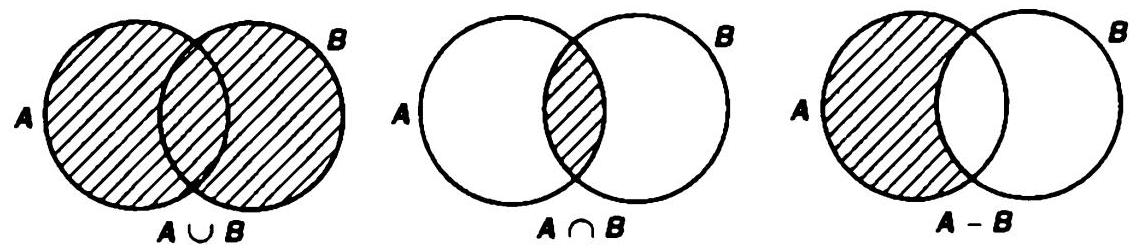
\includegraphics[width=1.0\textwidth]{images/1.1.jpg}
\end{center}
\hspace*{3em} 

Figure 1.1

\section*{Rules of Set Theory}

Given several sets, one may form new sets by applying the set-theoretic operations to them. As in algebra, one uses parentheses to indicate in what order the operations are to be performed. For example, \(A \cup  \left( {B \cap  C}\right)\) denotes the union of the two sets \(A\) and \(B \cap  C\) , while \(\left( {A \cup  B}\right)  \cap  C\) denotes the intersection of the two sets \(A \cup  B\) and \(C\) . The sets thus formed are quite different, as Figure 1.2 shows.

\begin{center}
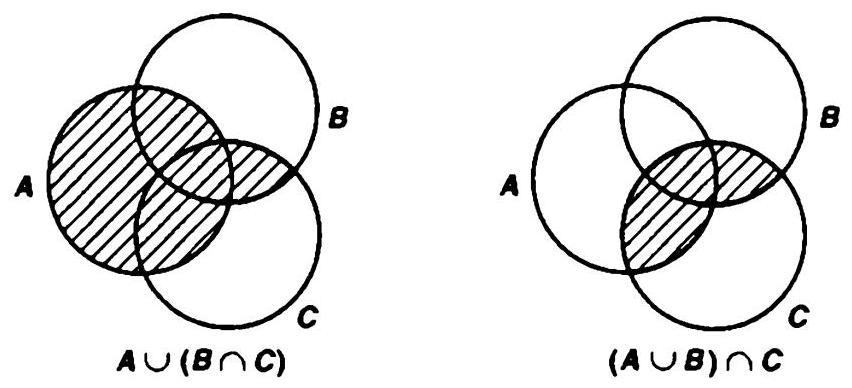
\includegraphics[width=0.7\textwidth]{images/1.2.jpg}
\end{center}
\hspace*{3em} 

Figure 1.2

Sometimes different combinations of operations lead to the same set; when that happens, one has a rule of set theory. For instance, it is true that for any sets \(A,B\) , and \(C\) the equation

\[
A \cap  \left( {B \cup  C}\right)  = \left( {A \cap  B}\right)  \cup  \left( {A \cap  C}\right)
\]

holds. The equation is illustrated in Figure 1.3; the shaded region represents the set in question, as you can check mentally. This equation can be thought of as a ``\idx{Distributive laws for  and} distributive law'' for the operations \(\cap\) and \(\cup\) .

\begin{center}
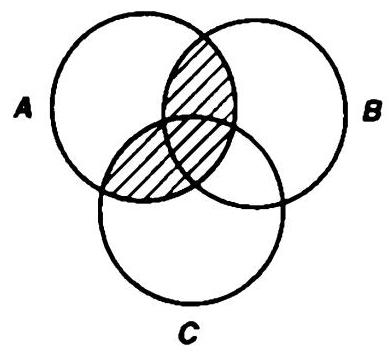
\includegraphics[width=0.3\textwidth]{images/1.3.jpg}
\end{center}
\hspace*{3em}

Figure 1.3

Other examples of set-theoretic rules include the \idx{Second coordinate of ordered pair} second ``distributive law,''

\[
A \cup  \left( {B \cap  C}\right)  = \left( {A \cup  B}\right)  \cap  \left( {A \cup  C}\right) ,
\]

and \idx{DeMorgan's laws},

\[
A - \left( {B \cup  C}\right)  = \left( {A - B}\right)  \cap  \left( {A - C}\right) ,
\]

\[
A - \left( {B \cap  C}\right)  = \left( {A - B}\right)  \cup  \left( {A - C}\right) .
\]

We leave it to you to check these rules. One can state other rules of set theory, but these are the most important ones. DeMorgan's laws are easier to remember if you verbalize them as follows:

The complement of the union equals the intersection of the complements.
The complement of the intersection equals the union of the complements.

\section*{Collections of Sets}

The objects belonging to a set may be of any sort. One can consider the set of all even integers, and the set of all blue-eyed people in Nebraska, and the set of all decks of playing cards in the world. Some of these are of limited mathematical interest, we admit! But the third example illustrates a point we have not yet mentioned: namely, that the objects belonging to a set may themselves be sets. For a deck of cards is itself a set, one consisting of pieces of pasteboard with certain standard designs printed on them. The set of all decks of cards in the world is thus a set whose elements are themselves sets (of pieces of pasteboard).

We now have another way to form new sets from old ones. Given a set \(A\) , we can consider sets whose elements are subsets of \(A\) . In particular, we can consider the set of all subsets of \(A\) . This set is sometimes denoted by the symbol \(\idxmath{P}{\(\mathcal{P}\left( A\right)\)} \mathcal{P}\left( A\right)\) and is called the \idx{power set} of \(A\) (for reasons to be explained later).

When we have a set whose elements are sets, we shall often refer to it as a \idx{collection} of sets and denote it by a script letter such as \(\mathcal{A}\) or \(\mathcal{B}\) . This device will help us in keeping things straight in arguments where we have to consider objects, and sets of objects, and collections of sets of objects, all at the same time. For example, we might use \(\mathcal{A}\) to denote the collection of all decks of cards in the world, letting an ordinary capital letter \(A\) denote a deck of cards and a lowercase letter \(a\) denote a single playing card.

A certain amount of care with notation is needed at this point. We make a distinction between the object \(a\) , which is an \idx{element of a set} \(A\) , and the one-element set \(\{ a\}\) , which is a subset of \(A\) . To illustrate, if \(A\) is the set \(\{ a,b,c\}\) , then the statements

\[
a \in  A,\;\{ a\}  \subset  A,\;\text{ and }\;\{ a\}  \in  \mathcal{P}\left( A\right)
\]

are all correct, but the statements \(\{ a\}  \in  A\) and \(a \subset  A\) are not.

\section*{Arbitrary Unions and Intersections}

We have already defined what we mean by the union and the intersection of two sets. There is no reason to limit ourselves to just two sets, for we can just as well form the union and intersection of arbitrarily many sets.

Given a collection \(\mathcal{A}\) of sets, the union of the elements of \(\mathcal{A}\) is defined by the equation

\[
\mathop{\bigcup }\limits_{{A \in  \mathcal{A}}}A = \{ x \mid  x \in  A\text{ for at least one }A \in  \mathcal{A}\} .
\]

The intersection of the elements of \(\mathcal{A}\) is defined by the equation

\[
\mathop{\bigcap }\limits_{{A \in  \mathcal{A}}}A = \{ x \mid  x \in  A\text{ for every }A \in  \mathcal{A}\} .
\]

There is no problem with these definitions if one of the elements of \(\mathcal{A}\) happens to be the empty set. But it is a bit tricky to decide what (if anything) these definitions mean if we allow \(\mathcal{A}\) to be the empty collection. Applying the definitions literally, we see that no element \(x\) satisfies the defining property for the union of the elements of \(\mathcal{A}\) . So it is reasonable to say that

\[
\mathop{\bigcup }\limits_{{A \in  A}}A = \varnothing
\]

if \(\mathcal{A}\) is empty On the other hand, every \(x\) satisfies (vacuously) the defining property for the intersection of the elements of \(\mathcal{A}\) . The question is, every \(x\) in what set? If one has a given large set \(X\) that is specified at the outset of the discussion to be one’s ``universe of discourse,'' and one considers only subsets of \(X\) throughout, it is reasonable to let

\[
\mathop{\bigcap }\limits_{{A \in  A}}A = X
\]

when \(\mathcal{A}\) is empty Not all mathematicians follow this convention, however. To avoid difficulty, we shall not define the intersection when \(\mathcal{A}\) is empty.

\section*{Cartesian Products}

There is yet another way of forming new sets from old ones; it involves the notion of an ``\idx{ordered pair}'' of objects. When you studied analytic geometry, the first thing you did was to convince yourself that after one has chosen an \(x\) -axis and a \(y\) -axis in the plane, every point in the plane can be made to correspond to a unique ordered pair(x, y)of real numbers. (In a more sophisticated treatment of geometry, the plane is more likely to be defined as the set of all ordered pairs of real numbers!)

The notion of ordered pair carries over to general sets. Given sets \(A\) and \(B\) , we define their \idx{Cartesian product: countably infinite} cartesian product \(A \times  B\) to be the set of all ordered pairs(a, b)for which \(a\) is an element of \(A\) and \(b\) is an element of \(B\) . Formally,

\[
A \times  B = \{ \left( {a,b}\right)  \mid  a \in  A\text{ and }b \in  B\} .
\]

This definition assumes that the concept of ``ordered pair'' is already given. It can be taken as a primitive concept, as was the notion of ``set''; or it can be given a definition in terms of the set operations already introduced. One definition in terms of set operations is expressed by the equation

\[
\left( {a,b}\right)  = \{ \{ a\} ,\{ a,b\} \} ;
\]

it defines the ordered pair(a, b)as a collection of sets. If \(a \neq  b\) , this definition says that (a, b)is a collection containing two sets, one of which is a one-element set and the other a two-element set. The \idx{first coordinate} of the ordered pair is defined to be the element belonging to both sets, and the second coordinate is the element belonging to only one of the sets. If \(a = b\) , then(a, b)is a collection containing only one set \(\{ a\}\) , since \(\{ a,b\}  =\)  \(\{ a,a\}  = \{ a\}\) in this case. Its first coordinate and second coordinate both equal the element in this single set.

I think it is fair to say that most mathematicians think of an ordered pair as a primitive concept rather than thinking of it as a collection of sets!

Let us make a comment on notation. It is an unfortunate fact that the notation(a, b) is firmly established in mathematics with two entirely different meanings. One meaning, as an ordered pair of objects, we have just discussed. The other meaning is the one you are familiar with from analysis; if \(a\) and \(b\) are real numbers, the symbol(a, b) is used to denote the \idx{interval} consisting of all numbers \(x\) such that \(a < x < b\) . Most of the time, this conflict in notation will cause no difficulty because the meaning will be clear from the context. Whenever a situation occurs where confusion is possible, we shall adopt a different notation for the ordered pair(a, b), denoting it by the symbol

instead.

\section*{Exercises}

1. Check the distributive laws for \(\cup\) and \(\cap\) and DeMorgan’s laws.

2. Determine which of the following statements are true for all sets \(A,B,C\) , and \(D\) . If a double implication fails, determine whether one or the other of the possible implications holds. If an equality fails, determine whether the statement becomes true if the ``equals'' symbol is replaced by one or the other of the inclusion symbols \(\subset\) or \(\supset\) .

(a) \(A \subset  B\) and \(A \subset  C \Leftrightarrow  A \subset  \left( {B \cup  C}\right)\) .

(b) \(A \subset  B\) or \(A \subset  C \Leftrightarrow  A \subset  \left( {B \cup  C}\right)\) .

(c) \(A \subset  B\) and \(A \subset  C \Leftrightarrow  A \subset  \left( {B \cap  C}\right)\) .

(d) \(A \subset  B\) or \(A \subset  C \Leftrightarrow  A \subset  \left( {B \cap  C}\right)\) .

(e) \(A - \left( {A - B}\right)  = B\) .

(f) \(A - \left( {B - A}\right)  = A - B\) .

(g) \(A \cap  \left( {B - C}\right)  = \left( {A \cap  B}\right)  - \left( {A \cap  C}\right)\) .

(h) \(A \cup  \left( {B - C}\right)  = \left( {A \cup  B}\right)  - \left( {A \cup  C}\right)\) .

(i) \(\left( {A \cap  B}\right)  \cup  \left( {A - B}\right)  = A\) .

(j) \(A \subset  C\) and \(B \subset  D \Rightarrow  \left( {A \times  B}\right)  \subset  \left( {C \times  D}\right)\) .

(k) The converse of (j).

(l) The converse of(j), assuming that \(A\) and \(B\) are nonempty.

(m) \(\left( {A \times  B}\right)  \cup  \left( {C \times  D}\right)  = \left( {A \cup  C}\right)  \times  \left( {B \cup  D}\right)\) .

(n) \(\left( {A \times  B}\right)  \cap  \left( {C \times  D}\right)  = \left( {A \cap  C}\right)  \times  \left( {B \cap  D}\right)\) .

(o) \(A \times  \left( {B - C}\right)  = \left( {A \times  B}\right)  - \left( {A \times  C}\right)\) .

(p) \(\left( {A - B}\right)  \times  \left( {C - D}\right)  = \left( {A \times  C - B \times  C}\right)  - A \times  D\) .

(q) \(\left( {A \times  B}\right)  - \left( {C \times  D}\right)  = \left( {A - C}\right)  \times  \left( {B - D}\right)\) .

3. (a) Write the contrapositive and converse of the following statement: “If \(x < 0\) , then \({x}^{2} - x > 0\) ,'' and determine which (if any) of the three statements are true.

(b) Do the same for the statement ``If \(x > 0\) , then \({x}^{2} - x > 0\) .''

4. Let \(A\) and \(B\) be sets of real numbers. Write the negation of each of the following statements:

(a) For every \(a \in  A\) , it is true that \({a}^{2} \in  B\) .

(b) For at least one \(a \in  A\) , it is true that \({a}^{2} \in  B\) .

(c) For every \(a \in  A\) , it is true that \({a}^{2} \notin  B\) .

(d) For at least one \(a \notin  A\) , it is true that \({a}^{2} \in  B\) .

5. Let \(\mathcal{A}\) be a nonempty collection of sets. Determine the truth of each of the following statements and of their converses:

(a) \(x \in  \mathop{\bigcup }\limits_{{A \in  \mathcal{A}}}A \Rightarrow  x \in  A\) for at least one \(A \in  \mathcal{A}\) .

(b) \(x \in  \mathop{\bigcup }\limits_{{A \in  \mathcal{A}}}A \Rightarrow  x \in  A\) for every \(A \in  \mathcal{A}\) .

(c) \(x \in  \mathop{\bigcap }\limits_{{A \in  \mathcal{A}}}A \Rightarrow  x \in  A\) for at least one \(A \in  \mathcal{A}\) .

(d) \(x \in  \mathop{\bigcap }\limits_{{A \in  \mathcal{A}}}A \Rightarrow  x \in  A\) for every \(A \in  \mathcal{A}\) .

6. Write the contrapositive of each of the statements of Exercise 5.

7. Given sets \(A,B\) , and \(C\) , express each of the following sets in terms of \(A,B\) , and \(C\) , using the symbols \(\cup  , \cap\) , and-.

\[
D = \{ x \mid  x \in  A\text{ and }\left( {x \in  B\text{ or }x \in  C}\right) \} ,
\]

\[
E = \{ x \mid  \left( {x \in  A\text{ and }x \in  B}\right) \text{ or }x \in  C\} ,
\]

\[
F = \{ x \mid  x \in  A\text{ and }\left( {x \in  B \Rightarrow  x \in  C}\right) \} .
\]

8. If a set \(A\) has two elements, show that \(\mathcal{P}\left( A\right)\) has four elements. How many elements does \(\mathcal{P}\left( A\right)\) have if \(A\) has one element? Three elements? No elements? Why is \(\mathcal{P}\left( A\right)\) called the power set of \(A\) ?

9. Formulate and prove DeMorgan's laws for arbitrary unions and intersections.

10. Let \(\idxmath{R}{\(\mathbb{R}\) (reals)} \mathbb{R}\) denote the set of real numbers. For each of the following subsets of \(\mathbb{R} \times  \mathbb{R}\) , determine whether it is equal to the cartesian product of two subsets of \(\mathbb{R}\) .

(a) \(\{ \left( {x,y}\right)  \mid  x\) is an integer \(\}\) .

(b) \(\{ \left( {x,y}\right)  \mid  0 < y \leq  1\}\) .

(c) \(\{ \left( {x,y}\right)  \mid  y > x\}\) .

(d) \(\{ \left( {x,y}\right)  \mid  x\) is not an integer and \(y\) is an integer \(\}\) .

(e) \(\left\{  {\left( {x,y}\right)  \mid  {x}^{2} + {y}^{2} < 1}\right\}\) .

\section*{§ 2 \idx{Function}s}

The concept of function is one you have seen many times already, so it is hardly necessary to remind you how central it is to all mathematics. In this section, we give the precise mathematical definition, and we explore some of the associated concepts.

A function is usually thought of as a rule that assigns to each element of a set \(A\) , an element of a set \(B\) . In calculus, a function is often given by a simple formula such as \(f\left( x\right)  = 3{x}^{2} + 2\) or perhaps by a more complicated formula such as

\[
f\left( x\right)  = \mathop{\sum }\limits_{{k = 1}}^{\infty }{x}^{k}
\]

One often does not even mention the sets \(A\) and \(B\) explicitly, agreeing to take \(A\) to be the set of all real numbers for which the rule makes sense and \(B\) to be the set of all real numbers.

As one goes further in mathematics, however, one needs to be more precise about what a function is. Mathematicians think of functions in the way we just described, but the definition they use is more exact. First, we define the following:

\begin{definition} A \idx{rule of assignment} is a subset \(r\) of the cartesian product \(\mathbf{C} \times  \mathbf{D}\) of two sets, having the property that each element of \(C\) appears as the first coordinate of at most one ordered pair belonging to \(r\) .


Thus, a subset \(r\) of \(C \times  D\) is a rule of assignment if

\[
\left\lbrack  {\left( {c,d}\right)  \in  r\text{ and }\left( {c,{d}^{\prime }}\right)  \in  r}\right\rbrack \Rightarrow  \left\lbrack  {d = {d}^{\prime }}\right\rbrack  .
\]

We think of \(r\) as a way of assigning, to the element \(c\) of \(C\) , the element \(d\) of \(D\) for which \(\left( {c,d}\right)  \in  r\) .

Given a rule of assignment \(r\) , the \idx{domain} of \(\mathrm{r}\) is defined to be the subset of \(C\) consisting of all first coordinates of elements of \(r\) , and the \idx{image} set of \(r\) is defined as the subset of \(D\) consisting of all second coordinates of elements of \(r\) . Formally,

\[
\text{ domain }r = \{ c \mid  \text{ there exists }d \in  D\text{ such that }\left( {c,d}\right)  \in  r\} \text{ , }
\]

\[
\text{ image }r = \{ d \mid  \text{ there exists }c \in  C\text{ such that }\left( {c,d}\right)  \in  r\} \text{ . }
\]
\end{definition}

Note that given a rule of assignment \(r\) , its domain and image are entirely determined. Now we can say what a function is.

\begin{definition} A function \(f\) is a rule of assignment \(r\) , together with a set \(B\) that contains the image set of \(r\) . The domain \(A\) of the rule \(r\) is also called the domain of the function \(f\) ; the image set of \(r\) is also called the image set of \(f\) ; and the set \(B\) is called the \idx{Range of a function} range of \(f{.}^{\dagger}\) .
\end{definition}

If \(f\) is a function having domain \(A\) and range \(B\) , we express this fact by writing

\[
f : A \rightarrow  B
\]

which is read `` \(f\) is a function from \(A\) to \(B\) ,'' or `` \(f\) is a \idx{mapping} from \(A\) into \(B\) ,'' or simply `` \(f\) maps \(A\) into \(B\) .'' One sometimes visualizes \(f\) as a geometric transformation physically carrying the points of \(A\) to points of \(B\) .

If \(f : A \rightarrow  B\) and if \(a\) is an element of \(A\) , we denote by \(f\left( a\right)\) the unique element of \(B\) that the rule determining \(f\) assigns to \(a\) ; it is called the \idx{Value of a function} value of \(f\) at \(a\) , or sometimes the image of \(a\) under \(f\) . Formally, if \(r\) is the rule of the function \(f\) , then \(f\left( a\right)\) denotes the unique element of \(B\) such that \(\left( {a,f\left( a\right) }\right)  \in  r\) .

Using this notation, one can go back to defining functions almost as one did before, with no lack of rigor. For instance, one can write (letting \(\mathbb{R}\) denote the real numbers)

``Let \(f\) be the function whose rule is \(\left\{  {\left( {x,{x}^{3} + 1}\right)  \mid  x \in  \mathbb{R}}\right\}\) and whose range is \(\mathbf{R}\) ,''

\section*{or one can equally well write}

``Let \(f : \mathbb{R} \rightarrow  \mathbb{R}\) be the function such that \(f\left( x\right)  = {x}^{3} + 1\) .''

Both sentences specify precisely the same function. But the sentence ``Let \(f\) be the function \(f\left( x\right)  = {x}^{3} + 1\) `` is no longer adequate for specifying a function because it specifies neither the domain nor the range of \(f\) .

\customfootnote{${}^{\dagger}$ Analysts are apt to use the word "range" to denote what we have called the "image set'' of \(f\). They avoid giving the set \(B\) a name.}


\begin{definition} If \(f : A \rightarrow  B\) and if \({A}_{0}\) is a subset of \(A\) , we define the restriction of \(f\) to \({A}_{0}\) to be the function mapping \({A}_{0}\) into \(B\) whose rule is

\[
\left\{  {\left( {a,f\left( a\right) }\right)  \mid  a \in  {A}_{0}}\right\}  \text{ . }
\]

It is denoted by \(f \mid  {A}_{0}\) , which is read `` \(f\) restricted to \({A}_{0}\) .''
\end{definition}


\begin{centeredblock}
\begin{example} Let \(\mathbb{R}\) denote the real numbers and let \({\bar{\mathbb{R}}}_{ + }\) denote the nonnegative reals. Consider the functions

\(f : \mathbb{R} \rightarrow  \mathbb{R}\;\) defined by \(\;f\left( x\right)  = {x}^{2},\)

\(g \cdot  {\overline{\mathbb{R}}}_{ + } \rightarrow  \mathbb{R}\;\) defined by \(\;g\left( x\right)  = {x}^{2},\)

\(h.\mathbb{R} \rightarrow  {\overline{\mathbb{R}}}_{ + }\;\) defined by \(\;h\left( x\right)  = {x}^{2}\) ,

\(k.{\overline{\mathbb{R}}}_{ + } \rightarrow  {\overline{\mathbb{R}}}_{ + }\;\) defined by \(\;k\left( x\right)  = {x}^{2}\) .

The function \(g\) is different from the function \(f\) because their rules are different subsets of \(\mathbb{R} \times  \mathbb{R}\) ; it is the restriction of \(f\) to the set \({\overline{\mathbb{R}}}_{ + }\) . The function \(h\) is also different from \(f\) , even though their rules are the same set, because the range specified for \(h\) is different from the range specified for \(f\) . The function \(k\) is different from all of these. These functions are pictured in Figure 2.1
\end{example}
\end{centeredblock}

\begin{center}
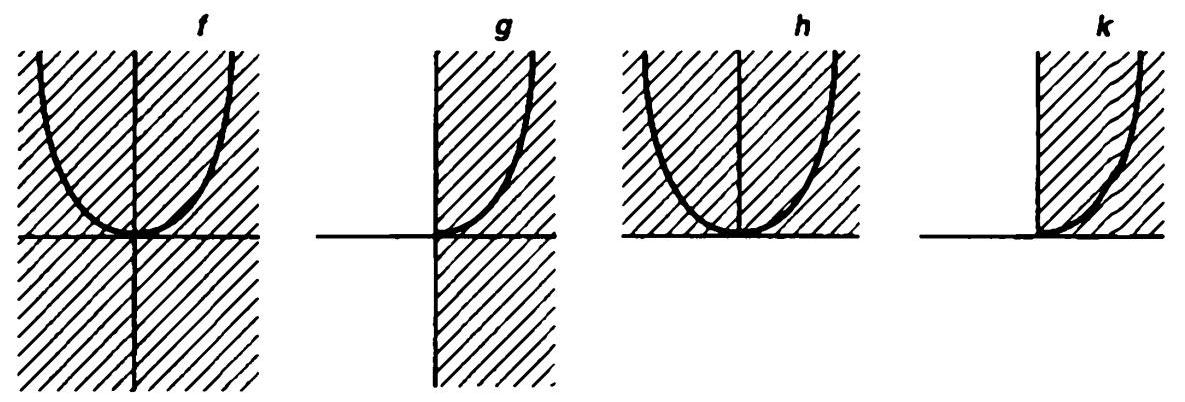
\includegraphics[width=1.0\textwidth]{images/2.1.jpg}
\end{center}
\hspace*{3em}

Figure 2.1

Restricting the domain of a function and changing its range are two ways of forming a new function from an old one. Another way is to form the \idx{Composite: of functions} composite of two functions.


\begin{definition}
    Given functions \(f : A \rightarrow  B\) and \(g : B \rightarrow  C\) , we define the composite \(g \circ  f\) of \(f\) and \(g\) as the function \(g \circ  f : A \rightarrow  C\) defined by the equation \(\left( {g \circ  f}\right) \left( a\right)  =\)  \(g\left( {f\left( a\right) }\right)\) .
\end{definition}


Formally, \(g \circ  f : A \rightarrow  C\) is the function whose rule is

\[
\{ \left( {a,c}\right)  \mid  \text{ For some }b \in  B,f\left( a\right)  = b\text{ and }g\left( b\right)  = c\} .
\]

We often picture the composite \(g \circ  f\) as involving a physical movement of the point \(a\) to the point \(f\left( a\right)\) , and then to the point \(g\left( {f\left( a\right) }\right)\) , as illustrated in Figure 2.2.

Note that \(g \circ  f\) is defined only when the range of \(f\) equals the domain of \(g\) .

\begin{center}
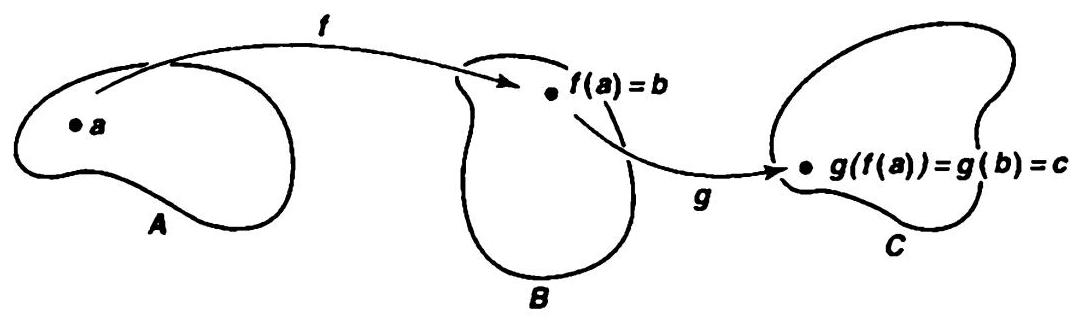
\includegraphics[width=1.0\textwidth]{images/2.2.jpg}
\end{center}
\hspace*{3em} 

Figure 2.2

\begin{example}
    The composite of the function \(f.\mathbb{R} \rightarrow  \mathbb{R}\) given by \(f\left( x\right)  = 3{x}^{2} + 2\) and the function \(g : \mathbb{R} \rightarrow  \mathbb{R}\) given by \(g\left( x\right)  = {5x}\) is the function \(g \circ  f : \mathbb{R} \rightarrow  \mathbb{R}\) given by
    \[
    \left( {g \circ  f}\right) \left( x\right)  = g\left( {f\left( x\right) }\right)  = g\left( {3{x}^{2} + 2}\right)  = 5\left( {3{x}^{2} + 2}\right) .
    \]
    The composite \(f \circ  g\) can also be formed in this case; it is the quite different function \(f \circ  g : \mathbb{R} \rightarrow  \mathbb{R}\) given by
    \[
    \left( {f \circ  g}\right) \left( x\right)  = f\left( {g\left( x\right) }\right)  = f\left( {5x}\right)  = 3{\left( 5x\right) }^{2} + 2.
    \]
\end{example}

\begin{definition}
    A function \(f : A \rightarrow  B\) is said to be injective (or one-to-one) if for each pair of distinct points of \(A\) , their images under \(f\) are distinct. It is said to be surjective (or \(f\) is said to map \(A\) onto \(B\) ) if every element of \(B\) is the image of some element of \(A\) under the function \(f\) . If \(f\) is both injective and surjective, it is said to be bijective (or is called a \idx{one-to-one correspondence}).
\end{definition}


More formally, \(f\) is injective if

\[
\left\lbrack  {f\left( a\right)  = f\left( {a}^{\prime }\right) }\right\rbrack \Rightarrow  \left\lbrack  {a = {a}^{\prime }}\right\rbrack  ,
\]

and \(f\) is surjective if

\[
\left\lbrack  {b \in  B}\right\rbrack \Rightarrow  \left\lbrack  {b = f\left( a\right) \text{ for at least one }a \in  A}\right\rbrack  .
\]

Injectivity of \(f\) depends only on the rule of \(f\) ; surjectivity depends on the range of \(f\) as well. You can check that the composite of two \idx{injective function}s is injective, and the composite of two \idx{surjective function}s is surjective; it follows that the composite of two \idx{bijective function}s is bijective.

If \(f\) is bijective, there exists a function from \(B\) to \(A\) called the \idx{Inverse function} inverse of \(f\) . It is denoted by \({f}^{-1}\) and is defined by letting \({f}^{-1}\left( b\right)\) be that unique element \(a\) of \(A\) for which \(f\left( a\right)  = b\) . Given \(b \in  B\) , the fact that \(f\) is surjective implies that there exists such an element \(a \in  A\) ; the fact that \(f\) is injective implies that there is only one such element \(a\) . It is easy to see that if \(f\) is bijective, \({f}^{-1}\) is also bijective.

\begin{example} Consider again the functions \(f,g,h\) , and \(k\) of Figure 2.1. The function \(f : \mathbb{R} \rightarrow  \mathbb{R}\) given by \(f\left( x\right)  = {x}^{2}\) is neither injective nor surjective. Its restriction \(g\) to the nonnegative reals is injective but not surjective. The function \(h : \mathbb{R} \rightarrow  \idxmath{R}{\({\mathbb{R}}_{ + }\)} {\mathbb{R}}_{ + }\) obtained from \(f\)

by changing the range is surjective but not injective. The function \(k{\overline{\mathbb{R}}}_{ + } \rightarrow  {\overline{\mathbb{R}}}_{ + }\) obtained from \(f\) by restricting the domain and changing the range is both injective and surjective, so it has an inverse. Its inverse is, of course, what we usually call the square-root function.
\end{example}

A useful criterion for showing that a given function \(f\) is bijective is the following, whose proof is left to the exercises:

\begin{lemma} Let \(f : A \rightarrow  B\) . If there are functions \(g : B \rightarrow  A\) and \(h : B \rightarrow  A\) such that \(g\left( {f\left( a\right) }\right)  = a\) for every \(a\) in \(A\) and \(f\left( {h\left( b\right) }\right)  = b\) for every \(b\) in \(B\) , then \(f\) is bijective and \(g = h = {f}^{-1}\) .
\end{lemma}

\begin{definition} Let \(f : A \rightarrow  B\) . If \({A}_{0}\) is a subset of \(A\) , we denote by \(f\left( {A}_{0}\right)\) the set of all images of points of \({A}_{0}\) under the function \(f\) ; this set is called the image of \({A}_{0}\) under \(f\) . Formally,

\[
f\left( {A}_{0}\right)  = \left\{  {b \mid  b = f\left( a\right) \text{ for at least one }a \in  {A}_{0}}\right\}  .
\]

On the other hand, if \({B}_{0}\) is a subset of \(B\) , we denote by \({f}^{-1}\left( {B}_{0}\right)\) the set of all elements of \(A\) whose images under \(f\) lie in \({B}_{0}\) ; it is called the \idx{preimage} of \({B}_{0}\) under \(f\) (or the ``\idx{counterimage},'' or the ``\idx{inverse image},'' of \({B}_{0}\) ). Formally,

\[
{f}^{-1}\left( {B}_{0}\right)  = \left\{  {a \mid  f\left( a\right)  \in  {B}_{0}}\right\}  .
\]

Of course, there may be no points \(a\) of \(A\) whose images lie in \({B}_{0}\) ; in that case, \({f}^{-1}\left( {B}_{0}\right)\) is empty.
\end{definition}

Note that if \(f : A \rightarrow  B\) is bijective and \({B}_{0} \subset  B\) , we have two meanings for the notation \({f}^{-1}\left( {B}_{0}\right)\) . It can be taken to denote the preimage of \({B}_{0}\) under the function \(f\) or to denote the image of \({B}_{0}\) under the function \({f}^{-1} : B \rightarrow  A\) . These two meanings give precisely the same subset of \(A\) , however, so there is, in fact, no ambiguity.

Some care is needed if one is to use the \(f\) and \({f}^{-1}\) notation correctly. The operation \({f}^{-1}\) , for instance, when applied to subsets of \(B\) , behaves very nicely; it preserves inclusions, unions, intersections, and differences of sets. We shall use this fact frequently. But the operation \(f\) , when applied to subsets of \(A\) , preserves only inclusions and unions. See Exercises 2 and 3.

As another situation where care is needed, we note that it is not in general true that \({f}^{-1}\left( {f\left( {A}_{0}\right) }\right)  = {A}_{0}\) and \(f\left( {{f}^{-1}\left( {B}_{0}\right) }\right)  = {B}_{0}\) . (See the following example.) The relevant rules, which we leave to you to check, are the following: If \(f : A \rightarrow  B\) and if \({A}_{0} \subset  A\) and \({B}_{0} \subset  B\) , then

\[
{A}_{0} \subset  {f}^{-1}\left( {f\left( {A}_{0}\right) }\right) \;\text{ and }\;f\left( {{f}^{-1}\left( {B}_{0}\right) }\right)  \subset  {B}_{0}.
\]

The first inclusion is an equality if \(f\) is injective, and the second inclusion is an equality if \(f\) is surjective.

\begin{example} Consider the function \(f : \mathbb{R} \rightarrow  \mathbb{R}\) given by \(f\left( x\right)  = 3{x}^{2} + 2\) (Figure 2.3) Let \(\left\lbrack  {a,b}\right\rbrack\) denote the closed interval \(a \leq  x \leq  b\) . Then

\[
{f}^{-1}\left( {f\left( \left\lbrack  {0,1}\right\rbrack  \right) }\right)  = {f}^{-1}\left( \left\lbrack  {2,5}\right\rbrack  \right)  = \left\lbrack  {-1,1}\right\rbrack  ,\;\text{ and }
\]

\[
f\left( {{f}^{-1}\left( \left\lbrack  {0,5}\right\rbrack  \right) }\right)  = f\left( \left\lbrack  {-1,1}\right\rbrack  \right)  = \left\lbrack  {2,5}\right\rbrack  .
\]
\end{example}

\begin{center}
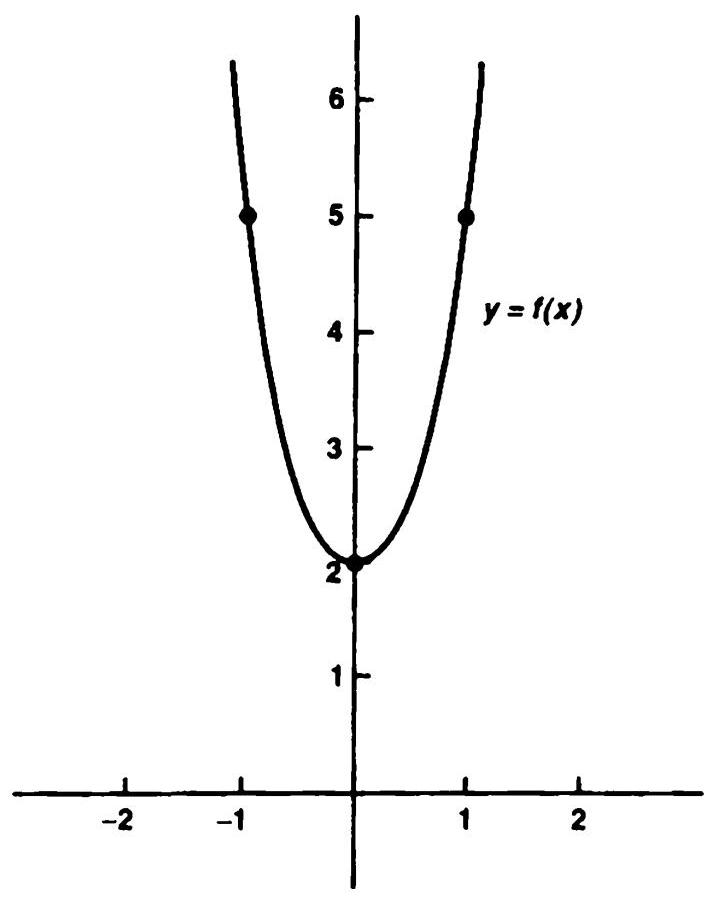
\includegraphics[width=0.6\textwidth]{images/2.3.jpg}
\end{center}
\hspace*{3em} 

Figure 2.3

\section*{Exercises}

1. Let \(f : A \rightarrow  B\) . Let \({A}_{0} \subset  A\) and \({B}_{0} \subset  B\) .

(a) Show that \({A}_{0} \subset  {f}^{-1}\left( {f\left( {A}_{0}\right) }\right)\) and that equality holds if \(f\) is injective.

(b) Show that \(f\left( {{f}^{-1}\left( {B}_{0}\right) }\right)  \subset  {B}_{0}\) and that equality holds if \(f\) is surjective.

2. Let \(f : A \rightarrow  B\) and let \({A}_{i} \subset  A\) and \({B}_{i} \subset  B\) for \(i = 0\) and \(i = 1\) . Show that \({f}^{ - }\) preserves inclusions, unions, intersections, and differences of sets:

(a) \({B}_{0} \subset  {B}_{1} \Rightarrow  {f}^{-1}\left( {B}_{0}\right)  \subset  {f}^{-1}\left( {B}_{1}\right)\) .

(b) \({f}^{-1}\left( {{B}_{0} \cup  {B}_{1}}\right)  = {f}^{-1}\left( {B}_{0}\right)  \cup  {f}^{-1}\left( {B}_{1}\right)\) .

(c) \({f}^{-1}\left( {{B}_{0} \cap  {B}_{1}}\right)  = {f}^{-1}\left( {B}_{0}\right)  \cap  {f}^{-1}\left( {B}_{1}\right)\) .

(d) \({f}^{-1}\left( {{B}_{0} - {B}_{1}}\right)  = {f}^{-1}\left( {B}_{0}\right)  - {f}^{-1}\left( {B}_{1}\right)\) .

Show that \(f\) preserves inclusions and unions only:

(e) \({A}_{0} \subset  {A}_{1} \Rightarrow  f\left( {A}_{0}\right)  \subset  f\left( {A}_{1}\right)\) .

(f) \(f\left( {{A}_{0} \cup  {A}_{1}}\right)  = f\left( {A}_{0}\right)  \cup  f\left( {A}_{1}\right)\) .

(g) \(f\left( {{A}_{0} \cap  {A}_{1}}\right)  \subset  f\left( {A}_{0}\right)  \cap  f\left( {A}_{1}\right)\) ; show that equality holds if \(f\) is injective.

(h) \(f\left( {{A}_{0} - {A}_{1}}\right)  \supset  f\left( {A}_{0}\right)  - f\left( {A}_{1}\right)\) ; show that equality holds if \(f\) is injective.

3. Show that (b), (c), (f), and (g) of Exercise 2 hold for arbitrary unions and intersections.

4. Let \(f : A \rightarrow  B\) and \(g : B \rightarrow  C\) .

(a) If \({C}_{0} \subset  C\) , show that \({\left( g \circ  f\right) }^{-1}\left( {C}_{0}\right)  = {f}^{-1}\left( {{g}^{-1}\left( {C}_{0}\right) }\right)\) .

(b) If \(f\) and \(g\) are injective, show that \(g \circ  f\) is injective.

(c) If \(g \circ  f\) is injective, what can you say about injectivity of \(f\) and \(g\) ?

(d) If \(f\) and \(g\) are surjective, show that \(g \circ  f\) is surjective.

(e) If \(g \circ  f\) is surjective, what can you say about surjectivity of \(f\) and \(g\) ?

(f) Summarize your answers to (b)-(e) in the form of a theorem.

5. In general, let us denote the \idx{identity function} for a set \(C\) by \({i}_{C}\) . That is, define \({i}_{C} : C \rightarrow  C\) to be the function given by the rule \({i}_{C}\left( x\right)  = x\) for all \(x \in  C\) . Given \(f : A \rightarrow  B\) , we say that a function \(g : B \rightarrow  A\) is a \idx{left inverse} for \(f\) if \(g \circ  f = {i}_{A}\) ; and we say that \(h : B \rightarrow  A\) is a \idx{right inverse} for \(f\) if \(f \circ  h = {i}_{B}\) .

(a) Show that if \(f\) has a left inverse, \(f\) is injective; and if \(f\) has a right inverse, \(f\) is surjective.

(b) Give an example of a function that has a left inverse but no right inverse.

(c) Give an example of a function that has a right inverse but no left inverse.

(d) Can a function have more than one left inverse? More than one right inverse?

(e) Show that if \(f\) has both a left inverse \(g\) and a right inverse \(h\) , then \(f\) is bijective and \(g = h = {f}^{-1}\) .

6. Let \(f : \mathbb{R} \rightarrow  \mathbb{R}\) be the function \(f\left( x\right)  = {x}^{3} - x\) . By restricting the domain and range of \(f\) appropriately, obtain from \(f\) a bijective function \(g\) . Draw the graphs of \(g\) and \({g}^{-1}\) . (There are several possible choices for \(g\) .)

\section*{§ 3 Relations}

A concept that is, in some ways, more general than that of function is the concept of a relation. In this section, we define what mathematicians mean by a relation, and we consider two types of relations that occur with great frequency in mathematics: \idx{equivalence relation}s and \idx{order relation}s. Order relations will be used throughout the book; equivalence relations will not be used until \(\$ {22}\) .

\begin{definition} A relation on a set \(A\) is a subset \(C\) of the cartesian product \(A \times  A\) .
\end{definition}


If \(C\) is a relation on \(A\) , we use the notation \({xCy}\) to mean the same thing as \(\left( {x,y}\right)  \in\)  \(C\) . We read it `` \(x\) is in the relation \(C\) to \(y\) .''

A rule of assignment \(r\) for a function \(f : A \rightarrow  A\) is also a subset of \(A \times  A\) . But it is a subset of a very special kind: namely, one such that each element of \(A\) appears as the first coordinate of an element of \(r\) exactly once. Any subset of \(A \times  A\) is a relation on \(A\) .

\begin{example} Let \(P\) denote the set of all people in the world, and define \(D \subset  P \times  P\) by the equation

\[
D = \{ \left( {x,y}\right)  \mid  x\text{ is a descendant of }y\} .
\]

Then \(D\) is a relation on the set \(P\) . The statements `` \(x\) is in the relation \(D\) to \(y\) `` and `` \(x\) is a descendant of \(y\) `` mean precisely the same thing, namely, that \(\left( {x,y}\right)  \in  D\) . Two other relations on \(P\) are the following

\[
B = \{ \left( {x,y}\right)  \mid  x\text{ has an ancestor who is also an ancestor of }y\} \text{ . }
\]

\[
S = \{ \left( {x,y}\right)  \mid  \text{ the parents of }x\text{ are the parents of }y\} \text{ . }
\]

We can call \(B\) the ``blood relation'' (pun intended), and we can call \(S\) the ``sibling relation.'' These three relations have quite different properties. The blood relationship is symmetric, for instance (if \(x\) is a blood relative of \(y\) , then \(y\) is a blood relative of \(x\) ), whereas the descendant relation is not. We shall consider these relations again shortly.
\end{example}

\section*{Equivalence Relations and Partitions}

An equivalence relation on a set \(A\) is a relation \(C\) on \(A\) having the following three properties:

(1) (Reflexivity) \({xCx}\) for every \(x\) in \(A\) .

(2) (Symmetry) If \({xCy}\) , then \({yCx}\) .

(3) (Transitivity) If \({xCy}\) and \({yCz}\) , then \({xCz}\) .

\begin{example} Among the relations defined in Example 1, the descendant relation \(D\) is neither reflexive nor symmetric, while the blood relation \(B\) is not transitive (I am not a blood relation to my wife, although my children are!) The sibling relation \(S\) is, however, an equivalence relation, as you may check.
\end{example}

There is no reason one must use a capital letter-or indeed a letter of any sort-to denote a relation, even though it is a set. Another symbol will do just as well. One symbol that is frequently used to denote an equivalence relation is the ``tilde'' symbol \(\sim\) . Stated in this notation, the properties of an equivalence relation become

(1) \(x \sim  x\) for every \(x\) in \(A\) .

(2) If \(x \sim  y\) , then \(y \sim  x\) .

(3) If \(x \sim  y\) and \(y \sim  z\) , then \(x \sim  z\) .

There are many other symbols that have been devised to stand for particular equivalence relations; we shall meet some of them in the pages of this book.

Given an equivalence relation \(\sim\) on a set \(A\) and an element \(x\) of \(A\) , we define a certain subset \(E\) of \(A\) , called the \idx{equivalence class} determined by \(x\) , by the equation

\[
E = \{ y \mid  y \sim  x\} .
\]

Note that the equivalence class \(E\) determined by \(x\) contains \(x\) , since \(x \sim  x\) . Equivalence classes have the following property:

\begin{lemma} Two equivalence classes \(E\) and \({E}^{\prime }\) are either disjoint or equal
\end{lemma}

\begin{proof}Let \(E\) be the equivalence class determined by \(x\) , and let \({E}^{\prime }\) be the equivalence class determined by \({x}^{\prime }\) . Suppose that \(E \cap  {E}^{\prime }\) is not empty; let \(y\) be a point of \(E \cap  {E}^{\prime }\) . See Figure 3.1. We show that \(E = {E}^{\prime }\) .
\begin{center}
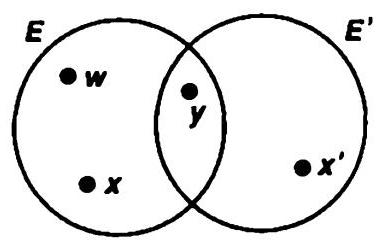
\includegraphics[width=0.3\textwidth]{images/3.1.jpg}
\end{center}
\hspace*{3em} 

Figure 3.1

By definition, we have \(y \sim  x\) and \(y \sim  {x}^{\prime }\) . Symmetry allows us to conclude that \(x \sim  y\) and \(y \sim  {x}^{\prime }\) ; from transitivity it follows that \(x \sim  {x}^{\prime }\) . If now \(w\) is any point of \(E\) , we have \(w \sim  x\) by definition; it follows from another application of transitivity that \(w \sim  {x}^{\prime }\) . We conclude that \(E \subset  {E}^{\prime }\) .

The symmetry of the situation allows us to conclude that \({E}^{\prime } \subset  E\) as well, so that \(E = {E}^{\prime }\) .

Given an equivalence relation on a set \(A\) , let us denote by \(\mathcal{E}\) the collection of all the equivalence classes determined by this relation. The preceding lemma shows that distinct elements of \(\mathcal{E}\) are disjoint. Furthermore, the union of the elements of \(\mathcal{E}\) equals all of \(A\) because every element of \(A\) belongs to an equivalence class. The collection \(\varepsilon\) is a particular example of what is called a partition of \(A\) :
\end{proof}
\begin{definition} A \idx{partition of a set} \(A\) is a collection of disjoint nonempty subsets of \(A\) whose union is all of \(A\) .
\end{definition}


Studying equivalence relations on a set \(A\) and studying partitions of \(A\) are really the same thing. Given any partition \(\mathcal{D}\) of \(A\) , there is exactly one equivalence relation on \(A\) from which it is derived.

The proof is not difficult. To show that the partition \(\mathcal{D}\) comes from some equivalence relation, let us define a relation \(C\) on \(A\) by setting \({xCy}\) if \(x\) and \(y\) belong to the same element of \(\mathcal{D}\) . Symmetry of \(C\) is obvious; reflexivity follows from the fact that the union of the elements of \(\mathcal{D}\) equals all of \(A\) ; transitivity follows from the fact that distinct elements of \(\mathcal{D}\) are disjoint It is simple to check that the collection of equivalence classes determined by \(C\) is precisely the collection \(\mathcal{D}\) .

To show there is only one such equivalence relation, suppose that \({C}_{1}\) and \({C}_{2}\) are two equivalence relations on \(A\) that give rise to the same collection of equivalence classes \(\mathcal{D}\) . Given \(x \in  A\) , we show that \(y{C}_{1}x\) if and only if \(y{C}_{2}x\) , from which we conclude that \({C}_{1} = {C}_{2}\) . Let \({E}_{1}\) be the equivalence class determined by \(x\) relative to the relation \({C}_{1}\) ; let \({E}_{2}\) be the equivalence class determined by \(x\) relative to the relation \({C}_{2}\) . Then \({E}_{1}\) is an element of \(\mathcal{D}\) , so that it must equal the unique element \(D\) of \(\mathcal{D}\) that contains \(x\) . Similarly, \({E}_{2}\) must equal \(D\) . Now by definition, \({E}_{1}\) consists of all \(y\) such that \(y{C}_{1}x\) ; and \({E}_{2}\) consists of all \(y\) such that \(y{C}_{2}x\) . Since \({E}_{1} = D = {E}_{2}\) , our result is proved.

\begin{example} Define two points in the plane to be equivalent if they lie at the same distance from the ongin. Reflexivity, symmetry, and transitivity hold trivially. The collection \(\varepsilon\) of equivalence classes consists of all circles centered at the origin, along with the set consisting of the origin alone.
\end{example}

\begin{example} Define two points of the plane to be equivalent if they have the same \(y\) -coordinate. The collection of equivalence classes is the collection of all straight lines in the plane parallel to the \(x\) -axis.
\end{example}

\begin{example} Let \(\mathcal{L}\) be the collection of all straight lines in the plane parallel to the line \(y =  - x\) . Then \(\mathcal{L}\) is a partition of the plane, since each point lies on exactly one such line. The partition \(\mathcal{L}\) comes from the equivalence relation on the plane that declares the points \(\left( {{x}_{0},{y}_{0}}\right)\) and \(\left( {{x}_{1},{y}_{1}}\right)\) to be equivalent if \({x}_{0} + {y}_{0} = {x}_{1} + {y}_{1}\) .
\end{example}

\begin{example} Let \({\mathcal{L}}^{\prime }\) be the collection of all straight lines in the plane. Then \({\mathcal{L}}^{\prime }\) is not a partition of the plane, for distinct elements of \({\mathcal{L}}^{\prime }\) are not necessarily disjoint; two lines may intersect without being equal.
\end{example}

\section*{Order Relations}

A relation \(C\) on a set \(A\) is called an order relation (or a \idx{simple order}, or a \idx{linear order}) if it has the following properties:

(1) (\idx{Comparability: of cardinalities} Comparability) For every \(x\) and \(y\) in \(A\) for which \(x \neq  y\) , either \({xCy}\) or \({yCx}\) .

(2) (Nonreflexivity) For no \(x\) in \(A\) does the relation \({xCx}\) hold.

(3) (Transitivity) If \({xCy}\) and \({yCz}\) , then \({xCz}\) .

Note that property (1) does not by itself exclude the possibility that for some pair of elements \(x\) and \(y\) of \(A\) , both the relations \({xCy}\) and \({yCx}\) hold (since ``or'' means ``one or the other, or both''). But properties (2) and (3) combined do exclude this possibility; for if both \({xCy}\) and \({yCx}\) held, transitivity would imply that \({xCx}\) , contradicting nonreflexivity.

\begin{example} Consider the relation on the real line consisting of all pairs(x, y)of real numbers such that \(x < y\) . It is an order relation, called the ``usual order relation,'' on the real line. A less familiar order relation on the real line is the following: Define \({xCy}\) if \({x}^{2} < {y}^{2}\) , or if \({x}^{2} = {y}^{2}\) and \(x < y\) . You can check that this is an order relation.
\end{example}

\begin{example} Consider again the relationships among people given in Example 1. The blood relation \(B\) satisfies none of the properties of an order relation, and the sibling relation \(S\) satisfies only (3). The descendant relation \(D\) does somewhat better, for it satisfies both (2) and (3); however, comparability still fails. Relations that satisfy (2) and (3) occur often enough in mathematics to be given a special name. They are called strict \idx{partial order} relations; we shall consider them later (see \(§{11}\) ).
\end{example}

As the tilde, \(\sim\) , is the generic symbol for an equivalence relation, the ``less than'' symbol, \(<\) , is commonly used to denote an order relation. Stated in this notation, the properties of an order relation become

(1) If \(x \neq  y\) , then either \(x < y\) or \(y < x\) .

(2) If \(x < y\) , then \(x \neq  y\) .

(3) If \(x < y\) and \(y < z\) , then \(x < z\) .

We shall use the notation \(x \leq  y\) to stand for the statement ``either \(x < y\) or \(x = y\) ``; and we shall use the notation \(y > x\) to stand for the statement `` \(x < y\) .'' We write \(x < y < z\) to mean `` \(x < y\) and \(y < z\) .''

\begin{definition} If \(X\) is a set and \(<\) is an order relation on \(X\) , and if \(a < b\) , we use the notation(a, b)to denote the set

\[
\{ x \mid  a < x < b\} \text{ ; }
\]

it is called an \idx{open interval} in \(X\) . If this set is empty, we call a the \idx{immediate predecessor} of \(b\) , and we call \(b\) the \idx{immediate successor} of \(a\) .
\end{definition}


\begin{definition} Suppose that \(A\) and \(B\) are two sets with order relations \({ < }_{A}\) and \({ < }_{B}\) respectively. We say that \(A\) and \(B\) have the same \idx{order type} if there is a bijective correspondence between them that preserves order; that is, if there exists a bijective function \(f : A \rightarrow  B\) such that

\[
{a}_{1}{ < }_{A}{a}_{2} \Rightarrow  f\left( {a}_{1}\right) { < }_{B}f\left( {a}_{2}\right) .
\]
\end{definition}


\begin{example} The interval(-1,1)of real numbers has the same order type as the set \(\mathbb{R}\) of real numbers itself, for the function \(f : \left( {-1,1}\right)  \rightarrow  \mathbb{R}\) given by

\[
f\left( x\right)  = \frac{x}{1 - {x}^{2}}
\]

is an order-preserving bijective correspondence, as you can check. It is pictured in Figure 3.2.
\end{example}

\begin{example} The subset \(A = \{ 0\}  \cup  \left( {1,2}\right)\) of \(\mathbb{R}\) has the same order type as the subset

\[
\lbrack 0,1) = \{ x \mid  0 \leq  x < 1\}
\]

of \(\mathbb{R}\) . The function \(f : A \rightarrow  \lbrack 0,1)\) defined by

\[
f\left( 0\right)  = 0,
\]

\[
f\left( x\right)  = x - 1\;\text{ for }x \in  \left( {1,2}\right)
\]

is the required order-preserving correspondence.
\end{example}

One interesting way of defining an order relation, which will be useful to us later in dealing with some examples, is the following:

\begin{center}
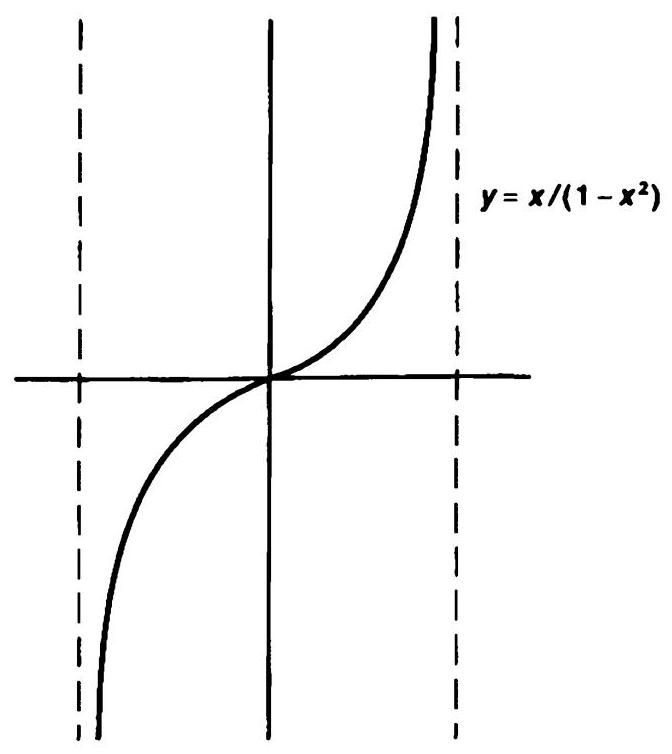
\includegraphics[width=0.6\textwidth]{images/3.2.jpg}
\end{center}
\hspace*{3em} 

Figure 3.2

\begin{definition} Suppose that \(A\) and \(B\) are two sets with order relations \({ < }_{A}\) and \({ < }_{B}\) respectively. Define an order relation \(<\) on \(A \times  B\) by defining

\[
{a}_{1} \times  {b}_{1} < {a}_{2} \times  {b}_{2}
\]

if \({a}_{1}{ < }_{A}{a}_{2}\) , or if \({a}_{1} = {a}_{2}\) and \({b}_{1}{ < }_{B}{b}_{2}\) . It is called the \idx{dictionary order} relation on \(A \times  B\) .
\end{definition}

Checking that this is an order relation involves looking at several separate cases; we leave it to you.

The reason for the choice of terminology is fairly evident. The rule defining \(<\) is the same as the rule used to order the words in the dictionary. Given two words, one compares their first letters and orders the words according to the order in which their first letters appear in the alphabet. If the first letters are the same, one compares their second letters and orders accordingly. And so on.


\begin{example} Consider the dictionary order on the plane \(\mathbb{R} \times  \mathbb{R}\) . In this order, the point \(p\) is less than every point lying above it on the vertical line through \(p\) , and \(p\) is less than every point to the right of this vertical line.
\end{example}

\begin{example} Consider the set \(\lbrack 0,1)\) of real numbers and the set \(\idxmath{Z}{\({\mathbb{Z}}_{ + }\)} {\idxmath{Z}{\(\mathbb{Z}\)} \mathbb{Z}}_{ + }\) of \idx{positive integers}, both in their usual orders; give \({\mathbb{Z}}_{ + } \times  \lbrack 0,1)\) the dictionary order. This set has the same order type as the set of nonnegative reals; the function

\[
f\left( {n \times  t}\right)  = n + t - 1
\]

is the required bijective order-preserving correspondence. On the other hand, the set \(\left( {0,1}\right)  \times  {\mathbb{Z}}_{ + }\) in the dictionary order has quite a different order type; for example, every element of this ordered set has an immediate successor. These sets are pictured in Figure 3.3.
\end{example}

\begin{center}
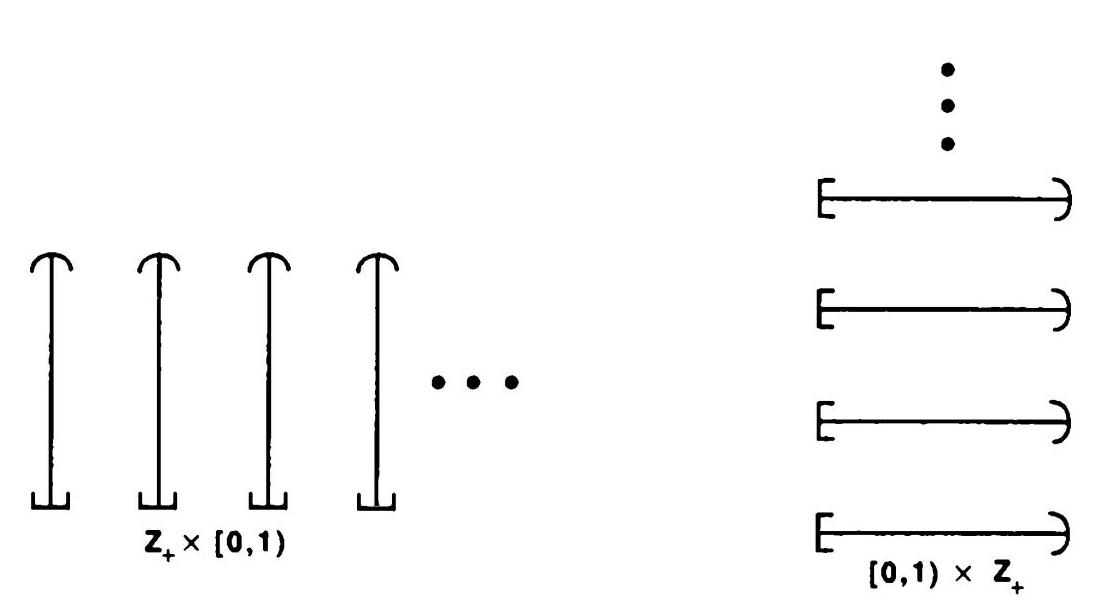
\includegraphics[width=1.0\textwidth]{images/3.3.jpg}
\end{center}
\hspace*{3em}

Figure 3.3

One of the properties of the real numbers that you may have seen before is the “least \idx{upper bound} property.” One can define this property for an arbitrary ordered set. First, we need some preliminary definitions.

Suppose that \(A\) is a set ordered by the relation \(<\) . Let \({A}_{0}\) be a subset of \(A\) . We say that the element \(b\) is the \idx{largest element} of \({A}_{0}\) if \(b \in  {A}_{0}\) and if \(x \leq  b\) for every \(x \in  {A}_{0}\) . Similarly, we say that \(a\) is the \idx{Smallest element of ordered set} smallest element of \({A}_{0}\) if \(a \in  {A}_{0}\) and if \(a \leq  x\) for every \(x \in  {A}_{0}\) . It is easy to see that a set has at most one largest element and at most one smallest element.

We say that the subset \({A}_{0}\) of \(A\) is \idx{bounded above} if there is an element \(b\) of \(A\) such that \(x \leq  b\) for every \(x \in  {A}_{0}\) ; the element \(b\) is called an upper bound for \({A}_{0}\) . If the set of all upper bounds for \({A}_{0}\) has a smallest element, that element is called the least upper bound, or the \idx{supremum}, of \({A}_{0}\) . It is denoted by sup \({A}_{0}\) ; it may or may not belong to \({A}_{0}\) . If it does, it is the largest element of \({A}_{0}\) .

Similarly, \({A}_{0}\) is \idx{bounded below} if there is an element \(a\) of \(A\) such that \(a \leq  x\) for every \(x \in  {A}_{0}\) ; the element \(a\) is called a \idx{lower bound} for \({A}_{0}\) . If the set of all lower bounds for \({A}_{0}\) has a largest element, that element is called the \idx{greatest lower bound}, or the \idx{infimum}, of \({A}_{0}\) . It is denoted by inf \({A}_{0}\) , it may or may not belong to \({A}_{0}\) . If it does, it is the smallest element of \({A}_{0}\) .

Now we can define the least upper bound property.

\begin{definition} An ordered set \(A\) is said to have the least upper bound property if every nonempty subset \({A}_{0}\) of \(A\) that is bounded above has a least upper bound. Analogously, the set \(A\) is said to have the greatest lower bound property if every nonempty subset \({A}_{0}\) of \(A\) that is bounded below has a greatest lower bound.
\end{definition}


We leave it to the exercises to show that \(A\) has the least upper bound property if and only if it has the greatest lower bound property.

\begin{example} Consider the set \(A = \left( {-1,1}\right)\) of real numbers in the usual order. Assuming the fact that the real numbers have the least upper bound property, it follows that the set \(A\) has the least upper bound property. For, given any subset of \(A\) having an upper bound in \(A\) , it follows that its least upper bound (in the real numbers) must be in \(A\) . For example, the subset \(\left\{  {-1/{2n} \mid  n \in  {\mathbb{Z}}_{ + }}\right\}\) of \(A\) , though it has no largest element, does have a least upper bound in \(A\) , the number 0 .

On the other hand, the set \(B = \left( {-1,0}\right)  \cup  \left( {0,1}\right)\) does not have the least upper bound property. The subset \(\left\{  {-1/{2n} \mid  n \in  {\mathbb{Z}}_{ + }}\right\}\) of \(B\) is bounded above by any element of(0,1), but it has no least upper bound in \(B\) .
\end{example}

\section*{Exercises}

Equivalence Relations

1. Define two points \(\left( {{x}_{0},{y}_{0}}\right)\) and \(\left( {{x}_{1},{y}_{1}}\right)\) of the plane to be equivalent if \({y}_{0} - {x}_{0}^{2} =\)  \({y}_{1} - {x}_{1}^{2}\) . Check that this is an equivalence relation and describe the equivalence classes

2. Let \(C\) be a relation on a set \(A\) . If \({A}_{0} \subset  A\) , define the restriction of \(C\) to \({A}_{0}\) to be the relation \(C \cap  \left( {{A}_{0} \times  {A}_{0}}\right)\) . Show that the restriction of an equivalence relation is an equivalence relation.

3. Here is a ``proof'' that every relation \(C\) that is both symmetric and transitive is also reflexive: ``Since \(C\) is symmetric, \({aCb}\) implies \({bCa}\) . Since \(C\) is transitive, \({aCb}\) and \({bCa}\) together imply \({aCa}\) , as desired.'' Find the flaw in this argument.

4. Let \(f : A \rightarrow  B\) be a surjective function. Let us define a relation on \(A\) by setting \({a}_{0} \sim  {a}_{1}\) if

\[
f\left( {a}_{0}\right)  = f\left( {a}_{1}\right) .
\]

(a) Show that this is an equivalence relation.

(b) Let \({A}^{ * }\) be the set of equivalence classes. Show there is a bijective correspondence of \({A}^{ * }\) with \(B\) .

5. Let \(S\) and \({S}^{\prime }\) be the following subsets of the plane.

\[
S = \{ \left( {x,y}\right)  \mid  y = x + 1\text{ and }0 < x < 2\} ,
\]

\[
{S}^{\prime } = \{ \left( {x,y}\right)  \mid  y - x\text{ is an integer }\} .
\]

(a) Show that \({S}^{\prime }\) is an equivalence relation on the real line and \({S}^{\prime } \supset  S\) . Describe the equivalence classes of \({S}^{\prime }\) .

(b) Show that given any collection of equivalence relations on a set \(A\) , their intersection is an equivalence relation on \(A\) .

(c) Describe the equivalence relation \(T\) on the real line that is the intersection of all equivalence relations on the real line that contain \(S\) . Describe the equivalence classes of \(T\) .

\section*{Order Relations}

6. Define a relation on the plane by setting

\[
\left( {{x}_{0},{y}_{0}}\right)  < \left( {{x}_{1},{y}_{1}}\right)
\]

if either \({y}_{0} - {x}_{0}^{2} < {y}_{1} - {x}_{1}^{2}\) , or \({y}_{0} - {x}_{0}^{2} = {y}_{1} - {x}_{1}^{2}\) and \({x}_{0} < {x}_{1}\) . Show that this is an order relation on the plane, and describe it geometrically.

7. Show that the restriction of an order relation is an order relation.

8. Check that the relation defined in Example 7 is an order relation.

9. Check that the dictionary order is an order relation.

10. (a) Show that the map \(f : \left( {-1,1}\right)  \rightarrow  \mathbb{R}\) of Example 9 is order preserving.

(b) Show that the equation \(g\left( y\right)  = {2y}/\left\lbrack  {1 + {\left( 1 + 4{y}^{2}\right) }^{1/2}}\right\rbrack\) defines a function \(g : \mathbb{R} \rightarrow  \left( {-1,1}\right)\) that is both a left and a right inverse for \(f\) .

11. Show that an element in an ordered set has at most one immediate successor and at most one immediate predecessor. Show that a subset of an ordered set has at most one smallest element and at most one largest element.

12. Let \({\mathbb{Z}}_{ + }\) denote the set of positive integers. Consider the following order relations on \({\mathbb{Z}}_{ + } \times  {\mathbb{Z}}_{ + }\) :

(i) The dictionary order.

(ii) \(\left( {{x}_{0},{y}_{0}}\right)  < \left( {{x}_{1},{y}_{1}}\right)\) if either \({x}_{0} - {y}_{0} < {x}_{1} - {y}_{1}\) , or \({x}_{0} - {y}_{0} = {x}_{1} - {y}_{1}\) and \({y}_{0} < {y}_{1}\) .

(iii) \(\left( {{x}_{0},{y}_{0}}\right)  < \left( {{x}_{1},{y}_{1}}\right)\) if either \({x}_{0} + {y}_{0} < {x}_{1} + {y}_{1}\) , or \({x}_{0} + {y}_{0} = {x}_{1} + {y}_{1}\) and \({y}_{0} < {y}_{1}\) .

In these order relations, which elements have immediate predecessors? Does the set have a smallest element? Show that all three order types are different.

13. Prove the following:

\begin{theorem} 
    If an ordered set \(A\) has the least upper bound property, then it has the greatest lower bound property.
\end{theorem}

14. If \(C\) is a relation on a set \(A\) , define a new relation \(D\) on \(A\) by letting \(\left( {b,a}\right)  \in  D\) if \(\left( {a,b}\right)  \in  C\) .

(a) Show that \(C\) is symmetric if and only if \(C = D\) .

(b) Show that if \(C\) is an order relation, \(D\) is also an order relation.

(c) Prove the converse of the theorem in Exercise 13.

15. Assume that the real line has the least upper bound property.

(a) Show that the sets

\[
\left\lbrack  {0,1}\right\rbrack = \{ x \mid  0 \leq  x \leq  1\} ,
\]

\[
\lbrack 0,1) = \{ x \mid  0 \leq  x < 1\rbrack
\]

have the least upper bound property.

(b) Does \(\left\lbrack  {0,1}\right\rbrack \times  \left\lbrack  {0,1}\right\rbrack\) in the dictionary order have the least upper bound property? What about \(\left\lbrack  {0,1}\right\rbrack \times  \lbrack 0,1)\) ? What about \(\lbrack 0,1) \times  \left\lbrack  {0,1}\right\rbrack\) ?

\section*{§ 4 The Integers and the Real Numbers}

Up to now we have been discussing what might be called the logical foundations for our study of topology-the elementary concepts of set theory. Now we turn to what we might call the mathematical foundations for our study-the integers and the real number system. We have already used them in an informal way in the examples and exercises of the preceding sections. Now we wish to deal with them more formally.

One way of establishing these foundations is to construct the real number system, using only the axioms of set theory-to build them with one's bare hands, so to speak. This way of approaching the subject takes a good deal of time and effort and is of greater logical than mathematical interest.

A second way is simply to assume a set of axioms for the real numbers and work from these axioms. In the present section, we shall sketch this approach to the real numbers. Specifically, we shall give a set of axioms for the real numbers and shall indicate how the familiar properties of real numbers and the integers are derived from them. But we shall leave most of the proofs to the exercises. If you have seen all this before, our description should refresh your memory. If not, you may want to work through the exercises in detail in order to make sure of your knowledge of the mathematical foundations.

First we need a definition from set theory.

\section*{Definition. A binary operation on a set \(A\) is a function \(f\) mapping \(A \times  A\) into \(A\) .}

When dealing with a \idx{binary operation} \(f\) on a set \(A\) , we usually use a notation different from the standard functional notation introduced in \(\$ 2\) . Instead of denoting the value of the function \(f\) at the point \(\left( {a,{a}^{\prime }}\right)\) by \(f\left( {a,{a}^{\prime }}\right)\) , we usually write the symbol for the function between the two coordinates of the point in question, writing the value of the function at \(\left( {a,{a}^{\prime }}\right)\) as \({af}{a}^{\prime }\) . Furthermore (just as was the case with relations), it is more common to use some symbol other than a letter to denote an operation. Symbols often used are the plus symbol +, the multiplication symbols - and -, and the asterisk \(*\) ; however, there are many others.

\section*{Assumption}

We assume there exists a set \(\mathbb{R}\) , called the set of real numbers, two binary operations + and \(\cdot\) on \(\mathbb{R}\) , called the addition and multiplication operations, respectively, and an order relation \(<\) on \(\mathbb{R}\) , such that the following properties hold:

Algebraic Properties

(l) \(\left( {x + y}\right)  + z = x + \left( {y + z}\right)\) ,

\(\left( {x \cdot  y}\right)  \cdot  z = x \cdot  \left( {y \cdot  z}\right)\) for all \(x,y,z\) in \(\mathbb{R}\) .

(2) \(x + y = y + x\) .

\(x \cdot  y = y \cdot  x\) for all \(x,y\) in \(\mathbb{R}\) .

(3) There exists a unique element of \(\mathbb{R}\) called zero, denoted by 0, such that \(x + 0 = x\) for all \(x \in  \mathbb{R}\) .

There exists a unique element of \(\mathbb{R}\) called one, different from 0 and denoted by 1, such that \(x \cdot  1 = x\) for all \(x \in  \mathbb{R}\) .

(4) For each \(x\) in \(\mathbb{R}\) , there exists a unique \(y\) in \(\mathbb{R}\) such that \(x + y = 0\) .

For each \(x\) in \(\mathbb{R}\) different from 0, there exists a unique \(y\) in \(\mathbb{R}\) such that \(x \cdot  y = 1\) .

(5) \(x \cdot  \left( {y + z}\right)  = \left( {x \cdot  y}\right)  + \left( {x \cdot  z}\right)\) for all \(x,y,z \in  \mathbb{R}\) .

A Mixed Algebraic and Order Property

(6) If \(x > y\) , then \(x + z > y + z\) .

If \(x > y\) and \(z > 0\) , then \(x \cdot  z > y \cdot  z\) .

\section*{Order Properties}

(7) The order relation \(<\) has the least upper bound property.

(8) If \(x < y\) , there exists an element \(z\) such that \(x < z\) and \(z < y\) .

From properties (1)-(5) follow the familiar ``laws of algebra.'' Given \(x\) , one denotes by \(- x\) that number \(y\) such that \(x + y = 0\) ; it is called the negative of \(x\) . One defines the subtraction operation by the formula \(z - x = z + \left( {-x}\right)\) . Similarly, given \(x \neq  0\) , one denotes by \(1/x\) that number \(y\) such that \(x \cdot  y = 1\) ; it is called the reciprocal of \(x\) . One defines the quotient \(z/x\) by the formula \(z/x = z \cdot  \left( {1/x}\right)\) . The usual laws of signs, and the rules for adding and multiplying fractions, follow as theorems. These laws of algebra are listed in Exercise 1 at the end of the section. We often denote \(xy\)  \(\operatorname{simplyby}{xy}\) .

When one adjoins property (6) to properties (I)-(5), one can prove the usual ``laws of inequalities,'' such as the following:

\[
\text{ If }x > y\text{ and }z < 0\text{ , then }x \cdot  z < y \cdot  z\text{ . }
\]

\[
- 1 < 0\text{ and }0 < 1\text{ . }
\]

The laws of inequalities are listed in Exercise 2.

We define a number \(x\) to be positive if \(x > 0\) , and to be negative if \(x < 0\) . We denote the positive reals by \({\mathbb{R}}_{ + }\) and the nonnegative reals (for reasons to be explained later) by \({\overline{\mathbb{R}}}_{ + }\) . Properties (1)-(6) are familiar properties in modern algebra. Any set with two binary operations satisfying (1)-(5) is called by algebraists afield; if the field has an order relation satisfying (6), it is called an \idx{ordered field}.

Properties (7) and (8), on the other hand, are familiar properties in topology. They involve only the order relation; any set with an order relation satisfying (7) and (8) is called by topologists a \idx{linear continuum}.

Now it happens that when one adjoins to the axioms for an ordered field [properties (l)-(6)] the axioms for a linear continuum [properties (7) and (8)], the resulting list contains some redundancies. Property (8), in particular, can be proved as a consequence of the others; given \(x < y\) one can show that \(z = \left( {x + y}\right) /\left( {1 + 1}\right)\) satisfies the requirements of (8). Therefore, in the standard treatment of the real numbers, properties (1)-(7) are taken as axioms, and property (8) becomes a theorem. We have included (8) in our list merely to emphasize the fact that it and the least upper bound property are the two crucial properties of the order relation for \(\mathbb{R}\) . From these two properties many of the topological properties of \(\mathbb{R}\) may be derived, as we shall see in Chapter 3.

Now there is nothing in this list as it stands to tell us what an integer is. We now define the integers, using only properties (1)-(6).

\begin{definition} A subset \(A\) of the real numbers is said to be inductive if it contains the number 1, and if for every \(x\) in \(A\) , the number \(x + 1\) is also in \(A\) . Let \(\mathcal{A}\) be the collection of all inductive subsets of \(\mathbb{R}\) . Then the set \({\mathbb{Z}}_{ + }\) of positive integers is defined by the equation


\[
{\mathbb{Z}}_{ + } = \mathop{\bigcap }\limits_{{A \in  A}}A
\]
\end{definition}

Note that the set \({\mathbb{R}}_{ + }\) of positive real numbers is inductive, for it contains 1 and the statement \(x > 0\) implies the statement \(x + 1 > 0\) . Therefore, \({\mathbb{Z}}_{ + } \subset  {\mathbb{R}}_{ + }\) , so the elements of \({\mathbb{Z}}_{ + }\) are indeed positive, as the choice of terminology suggests. Indeed, one sees readily that1is the smallest element of \({\mathbb{Z}}_{ + }\) , because the set of all real numbers \(x\) for which \(x \geq  1\) is inductive.

The basic properties of \({\mathbb{Z}}_{ + }\) , which follow readily from the definition, are the following:

(I) \({\mathbb{Z}}_{ + }\) is inductive.

(2) (\idx{Principle of induction}). If \(A\) is an \idx{inductive set} of positive integers, then \(A =\)  \({Z}_{ + }\) .

We define the set \(\mathbb{Z}\) of integers to be the set consisting of the positive integers \({\mathbb{Z}}_{ + }\) , the number 0, and the negatives of the elements of \({\mathbb{Z}}_{ + }\) . One proves that the sum, difference, and product of two integers are integers, but the quotient is not necessarily an integer. The set \(\mathbb{Q}\) of quotients of integers is called the set of \idx{rational number}s.

One proves also that, given the integer \(n\) , there is no integer \(a\) such that \(n < a <\)  \(n + 1\) .

If \(n\) is a positive integer, we use the symbol \({S}_{n}\) to denote the set of all positive integers less than \(n\) ; we call it a section of the positive integers. The set \({S}_{1}\) is empty, and \({S}_{n + 1}\) denotes the set of positive integers between1and \(n\) , inclusive. We also use the notation

\[
\{ 1,\ldots ,n\}  = {S}_{n + 1}
\]

for the latter set.

Now we prove two properties of the positive integers that may not be quite so familiar, but are quite useful. They may be thought of as alternative versions of the \idx{induction principle}.

\begin{theorem}[Well-ordering property] Every nonempty subset of \({\mathbb{Z}}_{ + }\) has a smallest element.
\end{theorem}
\begin{proof} We first prove that, for each \(n \in  {\mathbb{Z}}_{ + }\) , the following statement holds: Every nonempty subset of \(\{ 1,\ldots ,n\}\) has a smallest element.

Let \(A\) be the set of all positive integers \(\mathrm{n}\) for which this statement holds. Then \(A\) contains 1, since if \(n = 1\) , the only nonempty subset of \(\{ 1,\ldots ,n\}\) is the set \(\{ 1\}\) itself. Then, supposing \(A\) contains \(n\) , we show that it contains \(n + 1\) . So let \(C\) be a nonempty subset of the set \(\{ 1,\ldots ,n + 1\}\) . If \(C\) consists of the single element \(n + 1\) , then that element is the smallest element of \(C\) . Otherwise, consider the set \(C \cap  \{ 1,\ldots ,n\}\) , which is nonempty. Because \(n \in  A\) , this set has a smallest element, which will automatically be the smallest element of \(C\) also. Thus \(A\) is inductive, so we conclude that \(A = {\mathbb{Z}}_{ + }\) ; hence the statement is true for all \(n \in  {\mathbb{Z}}_{ + }\) .

Now we prove the theorem. Suppose that \(D\) is a nonempty subset of \({\mathbb{Z}}_{ + }\) . Choose an element \(n\) of \(D\) . Then the set \(A = D \cap  \{ 1,\ldots ,n\}\) is nonempty, so that \(A\) has a smallest element \(k\) . The element \(k\) is automatically the smallest element of \(D\) as well.
\end{proof}

\begin{theorem}[\idx{Strong induction principle}] Let \(A\) be a set of positive integers. Suppose that for each posiave integer \(n\) , the statement \({S}_{n} \subset  A\) implies the statement \(n \in  A\) . Then \(A = {\mathbb{Z}}_{ + }\) .
\end{theorem}

\begin{proof}If \(A\) does not equal all of \({\mathbb{Z}}_{ + }\) , let \(n\) be the smallest positive integer that is not in \(A\) . Then every positive integer less than \(n\) is in \(A\) , so that \({S}_{n} \subset  A\) . Our hypothesis implies that \(n \in  A\) , contrary to assumption.
Everything we have done up to now has used only the axioms for an ordered field, properties (1)-(6) of the real numbers. At what point do you need (7), the least upper bound axiom?

For one thing, you need the least upper bound axiom to prove that the set \({\mathbb{Z}}_{ + }\) of positive integers has no upper bound in \(\mathbb{R}\) . This is the \idx{Archimedean ordering} property of the real line. To prove it, we assume that \({\mathbb{Z}}_{ + }\) has an upper bound and derive a contradiction. If \({\mathbb{Z}}_{ + }\) has an upper bound, it has a least upper bound \(b\) . There exists \(n \in  {\mathbb{Z}}_{ + }\) such that \(n > b - 1\) ; for otherwise, \(b - 1\) would be an upper bound for \({\mathbb{Z}}_{ + }\) smaller than \(b\) . Then \(n + 1 > b\) , contrary to the fact that \(b\) is an upper bound for \({\mathbb{Z}}_{ + }\) .

The least upper bound axiom is also used to prove a number of other things about \(\mathbb{R}\) . It is used for instance to show that \(\mathbb{R}\) has the greatest lower bound property. It is also used to prove the existence of a unique positive square root \(\sqrt{x}\) for every positive real number. This fact, in turn, can be used to demonstrate the existence of real numbers that are not rational numbers; the number \(\sqrt{2}\) is an easy example.

We use the symbol 2 to denote \(l + l\) , the symbol 3 to denote \(2 + l\) , and so on through the standard symbols for the positive integers. It is a fact that this procedure assigns to each positive integer a unique symbol, but we never need this fact and shall not prove it.

Proofs of these properties of the integers and real numbers, along with a few other properties we shall need later, are outlined in the exercises that follow.
\end{proof}
\section*{Exercises}


1. Prove the following ``laws of algebra'' for \(\mathbb{R}\) , using only axioms (1)-(5)

(a) If \(x + y = x\) , then \(y = 0\) .

(b) \(0 \cdot  x = 0\) . [Hint: Compute \(\left( {x + 0}\right)  \cdot  x\) .]

(c) \(- 0 = 0\) .

(d) \(- \left( {-x}\right)  = x\) .

(e) \(x\left( {-y}\right)  =  - \left( {xy}\right)  = \left( {-x}\right) y\) .

(f) \(\left( {-1}\right) x =  - x\) .

(g) \(x\left( {y - z}\right)  = {xy} - {xz}\) .

(h) \(- \left( {x + y}\right)  =  - x - y; - \left( {x - y}\right)  =  - x + y\) .

(i) If \(x \neq  0\) and \(x \cdot  y = x\) , then \(y = 1\) .

(j) \(x/x = 1\) if \(x \neq  0\) .

(k) \(x/1 = x\) .

(l) \(x \neq  0\) and \(y \neq  0 \Rightarrow  {xy} \neq  0\) .

(m) \(\left( {1/y}\right) \left( {1/z}\right)  = 1/\left( {yz}\right)\) if \(y,z \neq  0\) .

(n) \(\left( {x/y}\right) \left( {w/z}\right)  = \left( {xw}\right) /\left( {yz}\right)\) if \(y,z \neq  0\) .

(o) \(\left( {x/y}\right)  + \left( {w/z}\right)  = \left( {{xz} + {wy}}\right) /\left( {yz}\right)\) if \(y,z \neq  0\) .

(p) \(x \neq  0 \Rightarrow  1/x \neq  0\) .

(q) \(1/\left( {w/z}\right)  = z/w\) if \(w,z \neq  0\) .

(r) \(\left( {x/y}\right) /\left( {w/z}\right)  = \left( {xz}\right) /\left( {yw}\right)\) if \(y,w,z \neq  0\) .

(s) \(\left( {ax}\right) /y = a\left( {x/y}\right)\) if \(y \neq  0\) .

(t) \(\left( {-x}\right) /y = x/\left( {-y}\right)  =  - \left( {x/y}\right)\) if \(y \neq  0\) .

2. Prove the following ``laws of inequalities'' for \(\mathbb{R}\) , using axioms (1)-(6) along with

the results of Exercise 1:

(a) \(x > y\) and \(w > z \Rightarrow  x + w > y + z\) .

(b) \(x > 0\) and \(y > 0 \Rightarrow  x + y > 0\) and \(x \cdot  y > 0\) .

(c) \(x > 0 \Leftrightarrow - x < 0\) .

(d) \(x > y \Leftrightarrow - x <  - y\) .

(e) \(x > y\) and \(z < 0 \Rightarrow  {xz} < {yz}\) .

(f) \(x \neq  0 \Rightarrow  {x}^{2} > 0\) , where \({x}^{2} = x \cdot  x\) .

(g) \(- 1 < 0 < 1\)

(h) \({xy} > 0 \Leftrightarrow  x\) and \(y\) are both positive or both negative.

(i) \(x > 0 \Rightarrow  1/x > 0\) .

(j) \(x > y > 0 \Rightarrow  1/x < 1/y\) .

(k) \(x < y \Rightarrow  x < \left( {x + y}\right) /2 < y\) .

3. (a) Show that if \(\mathcal{A}\) is a collection of inductive sets, then the intersection of the elements of \(\mathcal{A}\) is an inductive set.

(b) Prove the basic properties (l) and (2) of \({\mathbb{Z}}_{ + }\) .

4. (a) Prove by induction that given \(n \in  {\mathbb{Z}}_{ + }\) , every nonempty subset of \(\{ 1,\ldots ,n\rbrack\) has a largest element.

(b) Explain why you cannot conclude from (a) that every nonempty subset of \({\mathbb{Z}}_{ + }\) has a largest element.

5. Prove the following properties of \(\mathbb{Z}\) and \({\mathbb{Z}}_{ + }\) :

(a) \(a,b \in  {\mathbb{Z}}_{ + } \Rightarrow  a + b \in  {\mathbb{Z}}_{ + }\) . [Hint: Show that given \(a \in  {\mathbb{Z}}_{ + }\) , the set \(X = \left\{  {x \mid  x \in  \mathbb{R}\text{ and }a + x \in  {\mathbb{Z}}_{ + }}\right\}\) is inductive.

(b) \(a,b \in  {\mathbb{Z}}_{ + } \Rightarrow  a \cdot  b \in  {\mathbb{Z}}_{ + }\) .

(c) Show that \(a \in  {\mathbb{Z}}_{ + } \Rightarrow  a - 1 \in  {\mathbb{Z}}_{ + } \cup  \{ 0\}\) . [Hint: Let \(X = \{ x \mid  x \in  \mathbb{R}\) and \(x - 1 \in  {\mathbb{Z}}_{ + } \cup  \{ 0\}\) ; show that \(X\) is inductive.

(d) \(c,d \in  \mathbb{Z} \Rightarrow  c + d \in  \mathbb{Z}\) and \(c - d \in  \mathbb{Z}\) . [Hint. Prove it first for \(d = 1\) .\}

(e) \(c,d \in  \mathbb{Z} \Rightarrow  c \cdot  d \in  \mathbb{Z}\) .

6. Let \(a \in  \mathbb{R}\) . Define inductively

\[
{a}^{1} = a,
\]

\[
{a}^{n + 1} = {a}^{n} \cdot  a
\]

for \(n \in  {\mathbb{Z}}_{ + }\) . (See \(§7\) for a discussion of the process of \idx{inductive definition}.) Show that for \(n,m \in  {\mathbb{Z}}_{ + }\) and \(a,b \in  \mathbb{R}\) ,

\[
{a}^{n}{a}^{m} = {a}^{n + m},
\]

\[
{\left( {a}^{n}\right) }^{m} = {a}^{nm},
\]

\[
{a}^{m}{b}^{m} = {\left( ab\right) }^{m}.
\]

These are called the laws of exponents [Hint: For fixed \(n\) , prove the formulas by induction on \(m\) .\}

7. Let \(a \in  \mathbb{R}\) and \(a \neq  0\) . Define \({a}^{0} = 1\) , and for \(n \in  {\mathbb{Z}}_{ + },{a}^{-n} = 1/{a}^{n}\) . Show that the laws of exponents hold for \(a,b \neq  0\) and \(n,m \in  \mathbb{Z}\) .

8. (a) Show that \(\mathbb{R}\) has the greatest lower bound property.

(b) Show that \(\inf \left\{  {1/n \mid  n \in  {\mathbb{Z}}_{ + }}\right\} = 0\) .

(c) Show that given \(a\) with \(0 < a < 1\) , inf \(\left\{  {{a}^{n} \mid  n \in  {\mathbb{Z}}_{ + }}\right\} = 0\) . [Hint: Let \(h = \left( {1 - a}\right) /a\) , and show that \({\left( 1 + h\right) }^{n} \geq  1 + {nh}\) .]

9. (a) Show that every nonempty subset of \(\mathbb{Z}\) that is bounded above has a largest element.

(b) If \(x \notin  \mathbb{Z}\) , show there is exactly one \(n \in  \mathbb{Z}\) such that \(n < x < n + 1\) .

(c) If \(x - y > 1\) , show there is at least one \(n \in  \mathbb{Z}\) such that \(y < n < x\) .

(d) If \(y < x\) , show there is a rational number \(z\) such that \(y < z < x\) .

10. Show that every positive number \(a\) has exactly one positive square root, as follows:

(a) Show that if \(x > 0\) and \(0 \leq  h < 1\) , then

\[
{\left( x + h\right) }^{2} \leq  {x}^{2} + h\left( {{2x} + 1}\right) ,
\]

\[
{\left( x - h\right) }^{2} \geq  {x}^{2} - h\left( {2x}\right)
\]

(b) Let \(x > 0\) . Show that if \({x}^{2} < a\) , then \({\left( x + h\right) }^{2} < a\) for some \(h > 0\) ; and if \({x}^{2} > a\) , then \({\left( x - h\right) }^{2} > a\) for some \(h > 0\) .

(c) Given \(a > 0\) , let \(B\) be the set of all real numbers \(x\) such that \({x}^{2} < a\) . Show that \(B\) is bounded above and contains at least one positive number. Let \(b = \sup B\) ; show that \({b}^{2} = a\) .

(d) Show that if \(b\) and \(c\) are positive and \({b}^{2} = {c}^{2}\) , then \(b = c\) .

11. Given \(m \in  \mathbb{Z}\) , we say that \(m\) is even if \(m/2 \in  \mathbb{Z}\) , and \(m\) is odd otherwise.

(a) Show that if \(m\) is odd, \(m = {2n} + 1\) for some \(n \in  \mathbb{Z}\) . [Hint: Choose \(n\) so that \(n < m/2 < n + 1\) .\}

(b) Show that if \(p\) and \(q\) are odd, so are \(p \cdot  q\) and \({p}^{n}\) , for any \(n \in  {\mathbb{Z}}_{ + }\) .

(c) Show that if \(a > 0\) is rational, then \(a = m/n\) for some \(m,n \in  {\mathbb{Z}}_{ + }\) where not both \(m\) and \(n\) are even. [Hint: Let \(n\) be the smallest element of the set \(\left\{  {x \mid  x \in  {\mathbb{Z}}_{ + }\text{ and }x \cdot  a \in  {\mathbb{Z}}_{ + }}\right\}\) .

(d) Theorem. \(\sqrt{2}\) is irrational.

\section*{§ 5 Cartesian Products}

We have already defined what we mean by the cartesian product \(A \times  B\) of two sets. Now we introduce more general cartesian products.

\begin{definition} Let \(\mathcal{A}\) be a nonempty collection of sets. An \idx{indexing function} for \(\mathcal{A}\) is a surjective function \(f\) from some set \(J\) , called the \idx{index set}, to \(\mathcal{A}\) . The collection \(\mathcal{A}\) , together with the indexing function \(f\) , is called an indexed \idx{family of sets}. Given \(\alpha  \in  J\) , we shall denote the set \(f\left( \alpha \right)\) by the symbol \({A}_{\alpha }\) . And we shall denote the indexed family itself by the symbol

\[
{\left\{  {A}_{\alpha }\right\}  }_{\alpha  \in  J},
\]

which is read ``the family of all \({A}_{\alpha }\) , as \(\alpha\) ranges over \(J\) .'' Sometimes we write merely \(\left\{  {A}_{\alpha }\right\}\) , if it is clear what the index set is.
\end{definition}

Note that although an indexing function is required to be surjective, it is not required to be injective. It is entirely possible for \({A}_{\alpha }\) and \({A}_{\beta }\) to be the same set of \(\mathcal{A}\) , even though \(\alpha  \neq  \beta\) .


One way in which indexing functions are used is to give a new notation for arbitrary unions and intersections of sets. Suppose that \(f : J \rightarrow  \mathcal{A}\) is an indexing function for \(\mathcal{A}\) ; let \({A}_{\alpha }\) denote \(f\left( \alpha \right)\) . Then we define

\[
\mathop{\bigcup }\limits_{{\alpha  \in  J}}{A}_{\alpha } = \left\{  {x \mid  \text{ for at least one }\alpha  \in  J,x \in  {A}_{\alpha }}\right\}  ,
\]

and

\[
\mathop{\bigcap }\limits_{{\alpha  \in  J}}{A}_{\alpha } = \left\{  {x \mid  \text{ for every }\alpha  \in  J,x \in  {A}_{\alpha }}\right\}
\]

These are simply new notations for previously defined concepts; one sees at once (using the surjectivity of the index function) that the first equals the union of all the elements of \(\mathcal{A}\) and the second equals the intersection of all the elements of \(\mathcal{A}\) .

Two especially useful index sets are the set \(\{ 1,\ldots ,n\}\) of positive integers from 1 to \(n\) , and the set \({\mathbb{Z}}_{ + }\) of all positive integers. For these index sets, we introduce some special notation. If a collection of sets is indexed by the set \(\{ 1,\ldots ,n\}\) , we denote the indexed family by the symbol \(\left\{  {{A}_{1},\ldots ,{A}_{n}}\right\}\) , and we denote the union and intersection, respectively, of the members of this family by the symbols

\[
{A}_{1} \cup  \cdots  \cup  {A}_{n}\;\text{ and }\;{A}_{1} \cap  \cdots  \cap  {A}_{n}.
\]

In the case where the index set is the set \({\mathbb{Z}}_{ + }\) , we denote the indexed family by the symbol \(\left\{  {{A}_{1},{A}_{2},\ldots }\right\}\) , and the union and intersection by the respective symbols

\[
{A}_{1} \cup  {A}_{2} \cup  \cdots \;\text{ and }\;{A}_{1} \cap  {A}_{2} \cap  \cdots \text{ . }
\]

\begin{definition} Let \(m\) be a positive integer. Given a set \(X\) , we define an \(m\) -tuple of elements of \(X\) to be a function

\[
\mathbf{x} : \{ 1,\ldots ,m\}  \rightarrow  X.
\]

If \(\mathbf{x}\) is an \(m\) -tuple, we often denote the value of \(\mathbf{x}\) at \(i\) by the symbol \({x}_{i}\) rather than \(\mathbf{x}\left( i\right)\) and call it the ith coordinate of \(\mathbf{x}\) . And we often denote the function \(\mathbf{x}\) itself by the symbol

\[
\left( {{x}_{1},\ldots ,{x}_{m}}\right) \text{ . }
\]
\end{definition}


Now let \(\left\{  {{A}_{1},\ldots ,{A}_{m}}\right\}\) be a family of sets indexed with the set \(\{ 1,\ldots ,m\}\) . Let \(X =\)  \({A}_{1} \cup  \cdots  \cup  {A}_{m}\) . We define the cartesian product of this indexed family, denoted by

\[
\mathop{\prod }\limits_{{i = 1}}^{m}{A}_{i}\;\text{ or }\;{A}_{1} \times  \cdots  \times  {A}_{m}
\]

to be the set of all \(m\) -tuples \(\left( {{x}_{1},\ldots ,{x}_{m}}\right)\) of elements of \(X\) such that \({x}_{i} \in  {A}_{i}\) for each \(i\) .

\begin{example} We now have two definitions for the symbol \(A \times  B\) . One definition is, of course, the one given earlier, under which \(A \times  B\) denotes the set of all ordered pairs (a, b)such that \(a \in  A\) and \(b \in  B\) . The second definition, just given, defines \(A \times  B\) as the set of all functions \(\mathbf{x} : \{ 1,2\}  \rightarrow  A \cup  B\) such that \(\mathbf{x}\left( 1\right)  \in  A\) and \(\mathbf{x}\left( 2\right)  \in  B\) . There is an obvious bijective correspondence between these two sets, under which the ordered pair(a, b)corresponds to the function \(\mathbf{x}\) defined by \(\mathbf{x}\left( 1\right)  = a\) and \(\mathbf{x}\left( 2\right)  = b\) . Since we commonly denote this function \(\mathbf{x}\) in ``tuple notation'' by the symbol(a, b), the notation itself suggests the correspondence. Thus for the cartesian product of two sets, the general definition of cartesian product reduces essentially to the earlier one.
\end{example}

\begin{example} How does the cartesian product \(A \times  B \times  C\) differ from the cartesian products \(A \times  \left( {B \times  C}\right)\) and \(\left( {A \times  B}\right)  \times  {C}^{7}\) Very little. There are obvious bijective correspondences between these sets, indicated as follows

\[
\left( {a,b,c}\right)  \leftrightarrow  \left( {a,\left( {b,c}\right) }\right)  \leftrightarrow  \left( {\left( {a,b}\right) ,c}\right) .
\]
\end{example}

\begin{definition} Given a set \(X\) , we define an \(\omega\) -tuple of elements of \(X\) to be a function

\[
\mathbf{x} : {\mathbb{Z}}_{ + } \rightarrow  X
\]

we also call such a function a sequence, or an \idx{infinite sequence}, of elements of \(X\) . If \(\mathbf{x}\) is an \(\omega\) -tuple, we often denote the value of \(\mathbf{x}\) at \(i\) by \({x}_{i}\) rather than \(\mathbf{x}\left( i\right)\) , and call it the i th coordinate of \(x\) . We denote \(x\) itself by the symbol

\[
\left( {{x}_{1},{x}_{2},\ldots }\right) \;\text{ or }\;{\left( {x}_{n}\right) }_{n \in  {\mathbb{Z}}_{ + }}.
\]
\end{definition}


Now let \(\left\{  {{A}_{1},{A}_{2},\ldots }\right\}\) be a family of sets, indexed with the positive integers; let \(X\) be the union of the sets in this family. The cartesian product of this indexed family of sets, denoted by

\[
\mathop{\prod }\limits_{{i \in  {\mathbf{Z}}_{ + }}}{A}_{i}\;\text{ or }\;{A}_{1} \times  {A}_{2} \times  \cdots ,
\]

is defined to be the set of all \(\omega\) -tuples \(\left( {{x}_{1},{x}_{2},\ldots }\right)\) of elements of \(X\) such that \({x}_{i} \in  {A}_{i}\) for each \(i\) .

Nothing in these definitions requires the sets \({A}_{l}\) to be different from one another. Indeed, they may all equal the same set \(X\) In that case, the cartesian product \({A}_{1} \times\)  \(\cdots  \times  {A}_{m}\) is just the set of all \(m\) -tuples of elements of \(X\) , which we denote by \(\idxmath{X}{\({X}^{m}\)} {X}^{m}\) . Similarly, the product \({A}_{1} \times  {A}_{2} \times  \cdots\) is just the set of all \(\omega\) -tuples of elements of \(X\) , which we denote by \(\idxmath{X}{\({X}^{\omega }\)} {X}^{\omega }\) .

Later we will define the cartesian product of an arbitrary indexed family of sets.

\begin{example} If \(\mathbb{R}\) is the set of real numbers, then \({\mathbb{R}}^{m}\) denotes the set of all \(m\) -tuples of real numbers; it is often called euclidean m-space (although Euclid would never recognize it). Analogously, \(\idxmath{R}{\({\mathbb{R}}^{\omega }\)} {\mathbb{R}}^{\omega }\) is sometimes called ``infinite-dimensional \idx{euclidean space}''; it is the set of all \(\omega\) -tuples \(\left( {{x}_{1},{x}_{2},\ldots }\right)\) of real numbers, that is, the set of all functions \(\mathbf{x} : {\mathbb{Z}}_{ + } \rightarrow  \mathbb{R}\) .
\end{example}

\section*{Exercises}

1. Show there is a bijective correspondence of \(A \times  B\) with \(B \times  A\) .

2. (a) Show that if \(n > 1\) there is bijective correspondence of

\[
{A}_{1} \times  \cdots  \times  {A}_{n}\;\text{ with }\;\left( {{A}_{1} \times  \cdots  \times  {A}_{n - 1}}\right)  \times  {A}_{n}.
\]

(b) Given the indexed family \(\left\{  {{A}_{1},{A}_{2},\ldots }\right\}\) , let \({B}_{t} = {A}_{{2i} - 1} \times  {A}_{2i}\) for each positive integer \(i\) . Show there is bijective correspondence of \({A}_{1} \times  {A}_{2} \times  \cdots\) with \({B}_{1} \times  {B}_{2} \times  \cdots\)

3. Let \(A = {A}_{1} \times  {A}_{2} \times  \cdots\) and \(B = {B}_{1} \times  {B}_{2} \times  \cdots\) .

(a) Show that if \({B}_{i} \subset  {A}_{i}\) for all \(i\) , then \(B \subset  A\) . (Structly speaking, if we are given a function mapping the index set \({\mathbb{Z}}_{ + }\) into the union of the sets \({B}_{i}\) , we must change its range before it can be considered as a function mapping \({\mathbb{Z}}_{ + }\) into the union of the sets \({A}_{i}\) . We shall ignore this technicality when dealing with cartesian products).

(b) Show the converse of (a) holds if \(B\) is nonempty.

(c) Show that if \(A\) is nonempty, each \({A}_{t}\) is nonempty. Does the converse hold? (We will return to this question in the exercises of §19.)

(d) What is the relation between the set \(A \cup  B\) and the cartesian product of the sets \({A}_{i} \cup  {B}_{i}\) ? What is the relation between the set \(A \cap  B\) and the cartesian product of the sets \({A}_{i} \cap  {B}_{i}\) ?

4. Let \(m,n \in  {\mathbb{Z}}_{ + }\) . Let \(X \neq  \varnothing\) .

(a) If \(m \leq  n\) , find an injective map \(f : {X}^{m} \rightarrow  {X}^{n}\) .

(b) Find a bijective map \(g : {X}^{m} \times  {X}^{n} \rightarrow  {X}^{m + n}\) .

(c) Find an injective map \(h : {X}^{n} \rightarrow  {X}^{\omega }\) .

(d) Find a bijective map \(k : {X}^{n} \times  {X}^{\omega } \rightarrow  {X}^{\omega }\) .

(e) Find a bijective map \(l : {X}^{\omega } \times  {X}^{\omega } \rightarrow  {X}^{\omega }\) .

(f) If \(A \subset  B\) , find an injective map \(m : {\left( {A}^{\omega }\right) }^{n} \rightarrow  {B}^{\omega }\) .

5. Which of the following subsets of \({\mathbb{R}}^{\omega }\) can be expressed as the cartesian product of subsets of \(\mathbb{R}\) ?

(a) \(\left\{  {\mathbf{x} \mid  {x}_{i}\text{ is an integer for all }i}\right\}\) .

(b) \(\left\{  {\mathbf{x} \mid  {x}_{i} \geq  i\text{ for all }i}\right\}\) .

(c) \(\left\{  {\mathbf{x} \mid  {x}_{i}\text{ is an integer for all }i \geq  {100}}\right\}\) .

(d) \(\left\{  {x \mid  {x}_{2} = {x}_{3}}\right\}\) .

\section*{§ 6 \idx{Finite Set}s}

Finite sets and \idx{infinite set}s, \idx{countable set}s and \idx{uncountable set}s, these are types of sets that you may have encountered before. Nevertheless, we shall discuss them in this section and the next, not only to make sure you understand them thoroughly, but also to elucidate some particular points of logic that will arise later on. First we consider finite sets.

Recall that if \(n\) is a positive integer, we use \({S}_{n}\) to denote the set of positive integers less than \(n\) ; it is called a section of the positive integers. The sets \({S}_{n}\) are the prototypes for what we call the finite sets.

\begin{definition} A set is said to be finite if there is a bijective correspondence of \(A\) with some section of the positive integers. That is, \(A\) is finite if it is empty or if there is a bijection

\[
f : A \rightarrow  \{ 1,\ldots ,n\}
\]

for some positive integer \(n\) . In the former case, we say that \(A\) has \idx{Cardinality: comparability} cardinality 0; in the latter case, we say that \(A\) has cardinality \(n\) .
\end{definition}

For instance, the set \(\{ 1,\ldots ,n\}\) itself has cardinality \(n\) , for it is in bijective correspondence with itself under the identity function.

Now note carefully: We have not yet shown that the cardinality of a finite set is uniquely determined by the set. It is of course clear that the empty set must have cardinality zero. But as far as we know, there might exist bijective correspondences of a given nonempty set \(A\) with two different sets \(\{ 1,\ldots ,n\}\) and \(\{ 1,\ldots ,m\}\) . The possibility may seem ridiculous, for it is like saying that it is possible for two people to count the marbles in a box and come out with two different answers, both correct. Our experience with counting in everyday life suggests that such is impossible, and in fact this is easy to prove when \(n\) is a small number such as 1,2, or 3 . But a direct proof when \(n\) is 5 million would be impossibly demanding.

Even empirical demonstration would be difficult for such a large value of \(n\) . One might, for instance, construct an experiment by taking a freight car full of marbles and hiring 10 different people to count them independently. If one thinks of the physical problems involved, it seems likely that the counters would not all arrive at the same answer. Of course, the conclusion one could draw is that at least one person made a mistake. But that would mean assuming the correctness of the result one was trying to demonstrate empirically An alternative explanation could be that there do exist bijective correspondences between the given set of marbles and two different sections of the positive integers

In real life, we accept the first explanation. We simply take it on faith that our experience in counting comparatively small sets of objects demonstrates a truth that holds for arbitrarily large sets as well.

However, in mathematics (as opposed to real life), one does not have to take this statement on faith. If it is formulated in terms of the existence of bijective correspondences rather than in terms of the physical act of counting, it is capable of mathematical proof. We shall prove shortly that if \(n \neq  m\) , there do not exist bijective functions mapping a given set \(A\) onto both the sets \(\{ 1,\ldots ,n\}\) and \(\{ 1,\ldots ,m\}\) .

There are a number of other ``intuitively obvious'' facts about finite sets that are capable of mathematical proof, we shall prove some of them in this section and leave the rest to the exercises. Here is an easy fact to start with:

\begin{lemma} Let \(n\) be a positive integer. Let \(A\) be a set; let \({a}_{0}\) be an element of \(A\) . Then there exists a bijective correspondence \(f\) of the set \(A\) with the set \(\{ 1,\ldots ,n + 1\}\) if and only if there exists a bijective correspondence \(g\) of the set \(A - \left\{  {a}_{0}\right\}\) with the set \(\{ 1,\ldots ,n\}\) .
\end{lemma}

\begin{proof}There are two implications to be proved. Let us first assume that there is a bijective correspondence
\[
g : A - \left\{  {a}_{0}\right\} \rightarrow  \{ 1,\ldots ,n\} .
\]

We then define a function \(f : A \rightarrow  \{ 1,\ldots ,n + 1\}\) by setting

\[
f\left( x\right)  = g\left( x\right) \;\text{ for }x \in  A - \left\{  {a}_{0}\right\}  ,
\]

\[
f\left( {a}_{0}\right)  = n + 1
\]

One checks at once that \(f\) is bijective.

To prove the converse, assume there is a bijective correspondence

\[
f : A \rightarrow  \{ 1,\ldots ,n + 1\} .
\]

If \(f\) maps \({a}_{0}\) to the number \(n + 1\) , things are especially easy; in that case, the restriction \(f \mid  A - \left\{  {a}_{0}\right\}\) is the desired bijective correspondence of \(A - \left\{  {a}_{0}\right\}\) with \(\{ 1,\ldots ,n\}\) . Otherwise, let \(f\left( {a}_{0}\right)  = m\) , and let \({a}_{1}\) be the point of \(A\) such that \(f\left( {a}_{1}\right)  = n + 1\) . Then \({a}_{1} \neq  {a}_{0}\) . Define a new function

\[
h : A \rightarrow  \{ 1,\ldots ,n + 1\}
\]

by setting

\[
h\left( {a}_{0}\right)  = n + 1
\]

\[
h\left( {a}_{1}\right)  = m,
\]

\[
h\left( x\right)  = f\left( x\right) \;\text{ for }x \in  A - \left\{  {a}_{0}\right\} - \left\{  {a}_{1}\right\}  .
\]

See Figure 6.1. It is easy to check that \(h\) is a bijection.

Now we are back in the easy case; the restriction \(h \mid  A - \left\{  {a}_{0}\right\}\) is the desired bijection of \(A - \left\{  {a}_{0}\right\}\) with \(\{ 1,\ldots ,n\}\) .

\begin{center}
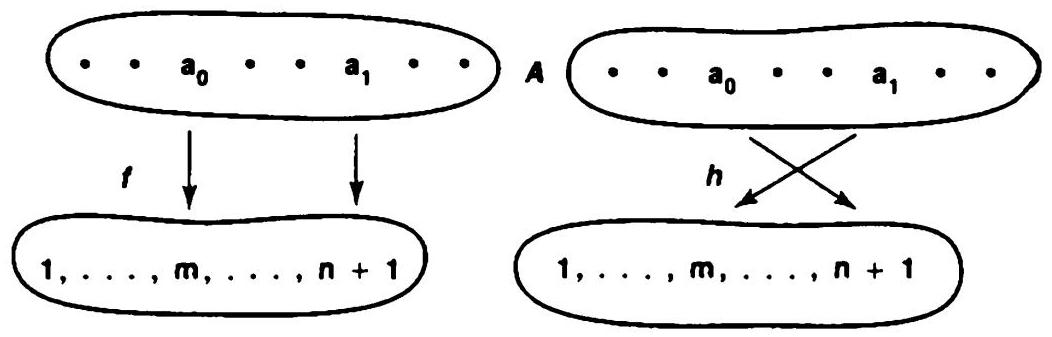
\includegraphics[width=0.9\textwidth]{images/6.1.jpg}
\end{center}
\hspace*{3em} 

Figure 6.1

From this lemma a number of useful con\idx{sequences} follow:
\end{proof}
\begin{theorem} Let \(A\) be a set; suppose that there exists a bijection \(f : A \rightarrow  \{ 1,\ldots ,n\}\) for some \(n \in  {\mathbb{Z}}_{ + }\) . Let \(B\) be a proper subset of \(A\) Then there exists no bijection \(g : B \rightarrow  \{ 1,\ldots ,n\}\) ; but (provided \(B \neq  \varnothing\) ) there does exist a bijection \(h : B \rightarrow  \{ 1,\ldots ,m\}\) for some \(m < n\) .
\end{theorem}

\begin{proof}The case in which \(B = \varnothing\) is trivial, for there cannot exist a bijection of the empty set \(B\) with the nonempty set \(\{ 1,\ldots ,n\}\) .
We prove the theorem ``by induction.'' Let \(C\) be the subset of \({\mathbb{Z}}_{ + }\) consisting of those integers \(n\) for which the theorem holds. We shall show that \(C\) is inductive. From this we conclude that \(C = {\mathbb{Z}}_{ + }\) , so the theorem is true for all positive integers \(n\) .

First we show the theorem is true for \(n = 1\) . In this case \(A\) consists of a single element \(\{ a\}\) , and its only proper subset \(B\) is the empty set.

Now assume that the theorem is true for \(n\) ; we prove it true for \(n + 1\) . Suppose that \(f : A \rightarrow  \{ 1,\ldots ,n + 1\}\) is a bijection, and \(B\) is a nonempty proper subset of \(A\) . Choose an element \({a}_{0}\) of \(B\) and an element \({a}_{1}\) of \(A - B\) . We apply the preceding lemma to conclude there is a bijection

\[
g : A - \left\{  {a}_{0}\right\} \rightarrow  \{ 1,\ldots ,n\} .
\]

Now \(B - \left\{  {a}_{0}\right\}\) is a proper subset of \(A - \left\{  {a}_{0}\right\}\) , for \({a}_{1}\) belongs to \(A - \left\{  {a}_{0}\right\}\) and not to \(B - \left\{  {a}_{0}\right\}\) . Because the theorem has been assumed to hold for the integer \(n\) , we conclude the following

(1) There exists no bijection \(h : B - \left\{  {a}_{0}\right\} \rightarrow  \{ 1,\ldots ,n\}\) .

(2) Either \(B - \left\{  {a}_{0}\right\} = \varnothing\) , or there exists a bijection

\[
k : B - \left\{  {a}_{0}\right\} \rightarrow  \{ 1,\ldots ,p\} \;\text{ for some }p < n.
\]

The preceding lemma, combined with (1), implies that there is no bijection of \(B\) with \(\{ 1,\ldots ,n + 1\}\) . This is the first half of what we wanted to proved. To prove the second half, note that if \(B - \left\{  {a}_{0}\right\} = \varnothing\) , there is a bijection of \(B\) with the set \(\{ 1\}\) ; while if \(B - \left\{  {a}_{0}\right\} \neq  \varnothing\) , we can apply the preceding lemma, along with (2), to conclude that there is a bijection of \(B\) with \(\{ 1,\ldots ,p + 1\}\) . In either case, there is a bijection of \(B\) with \(\{ 1,\ldots ,m\}\) for some \(m < n + 1\) , as desired. The induction principle now shows that the theorem is true for all \(n \in  {\mathbb{Z}}_{ + }\) .
\end{proof}
\begin{corollary} If \(A\) is finite, there is no bijection of \(A\) with a proper subset of itself.
\end{corollary}

\begin{proof}Assume that \(B\) is a proper subset of \(A\) and that \(f : A \rightarrow  B\) is a bijection. By assumption, there is a bijection \(g : A \rightarrow  \{ 1,\ldots ,n\}\) for some \(n\) . The composite \(g \circ  {f}^{-1}\) is then a bijection of \(B\) with \(\{ 1,\ldots ,n\}\) . This contradicts the preceding theorem.\end{proof}
\begin{corollary} \({\mathbb{Z}}_{ + }\) is not finite.
\end{corollary}

\begin{proof}The function \(f : {\mathbb{Z}}_{ + } \rightarrow  {\mathbb{Z}}_{ + } - \{ 1\}\) defined by \(f\left( n\right)  = n + 1\) is a bijection of \({\mathbb{Z}}_{ + }\) with a proper subset of itself.\end{proof}
\begin{corollary} The cardinality of a finite set \(A\) is uniquely determined by \(A\) .
\end{corollary}

\begin{proof}Let \(m < n\) . Suppose there are bijections
\[
f : A \rightarrow  \{ 1,\ldots ,n\}
\]

\[
g : A \rightarrow  \{ 1,\ldots ,m\} \text{ . }
\]

Then the composite

\[
g \circ  {f}^{-1} : \{ 1,\ldots ,n\}  \rightarrow  \{ 1,\ldots ,m\}
\]

is a bijection of the finite set \(\{ 1,\ldots ,n\}\) with a proper subset of itself, contradicting the corollary just proved.
\end{proof}
\begin{corollary} If \(B\) is a subset of the finite set \(A\) , then \(B\) is finite. If \(B\) is a proper subset of \(A\) , then the cardinality of \(B\) is less than the cardinality of \(A\) .
\end{corollary}

\begin{corollary} Let \(B\) be a nonempty set. Then the following are equivalent

(1) \(B\) is finite.

(2) There is a surjective function from a section of the positive integers onto \(B\) .

(3) There is an injective function from \(B\) into a section of the positive integers.
\end{corollary}

\begin{proof}(1) \(\Rightarrow\) (2). Since \(B\) is nonempty, there is, for some \(n\) , a bijective function \(f : \{ 1,\ldots ,n\}  \rightarrow  B\) .
\(\left( 2\right)  \Rightarrow  \left( 3\right)\) . If \(f : \{ 1,\ldots ,n\}  \rightarrow  B\) is surjective, define \(g : B \rightarrow  \{ 1,\ldots ,n\}\) by the equation

\[
g\left( b\right)  = \text{ smallest element of }{f}^{-1}\left( {\{ b\} }\right) .
\]

Because \(f\) is surjective, the set \({f}^{-1}\{ \left( b\right) \}\) is nonempty; then the well-ordering property of \({\mathbb{Z}}_{ + }\) tells us that \(g\left( b\right)\) is uniquely defined. The map \(g\) is injective, for if \(b \neq  {b}^{\prime }\) , then the sets \({f}^{-1}\left( {\{ b\} }\right)\) and \({f}^{-1}\left( \left\{  {b}^{\prime }\right\}  \right)\) are disjoint, so their smallest elements must be different.

\(\left( 3\right)  \Rightarrow  \left( 1\right)\) . If \(g : B \rightarrow  \{ 1,\ldots ,n\}\) is injective, then changing the range of \(g\) gives a bijection of \(B\) with a subset of \(\{ 1,\ldots ,n\}\) . It follows from the preceding corollary that \(B\) is finite.
\end{proof}
\begin{corollary} Finite unions and finite cartesian products of finite sets are finite.
\end{corollary}

\begin{proof}We first show that if \(A\) and \(B\) are finite, so is \(A \cup  B\) . The result is trivial if \(A\) or \(B\) is empty. Otherwise, there are bijections \(f : \{ 1,\ldots ,m\}  \rightarrow  \mathbf{A}\) and \(g\) : \(\{ 1,\ldots ,n\}  \rightarrow  B\) for some choice of \(m\) and \(n\) . Define a function \(h.\{ 1,\ldots ,m +\)  \(n\}  \rightarrow  A \cup  B\) by setting \(h\left( i\right)  = f\left( i\right)\) for \(i = 1,2,\ldots ,m\) and \(h\left( i\right)  = g\left( {i - m}\right)\) for \(i = m + 1,\ldots ,m + n\) . It is easy to check that \(h\) is surjective, from which it follows that \(A \cup  B\) is finite.
Now we show by induction that \idx{Finiteness: of cartesian products} finiteness of the sets \({A}_{1},\ldots ,{A}_{n}\) implies finiteness of their union. This result is trivial for \(n = 1\) Assuming it true for \(n - 1\) , we note that \({A}_{1} \cup  \cdots  \cup  {A}_{n}\) is the union of the two finite sets \({A}_{1} \cup  \cdots  \cup  {A}_{n - 1}\) and \({A}_{n}\) , so the result of the preceding paragraph applies.

Now we show that the cartesian product of two finite sets \(A\) and \(B\) is finite. Given \(a \in  A\) , the set \(\{ a\}  \times  B\) is finite, being in bijective correspondence with \(B\) . The set \(A \times  B\) is the union of these sets; since there are only finitely many of them, \(A \times  B\) is a finite union of finite sets and thus finite.

To prove that the product \({A}_{1} \times  \cdots  \times  {A}_{n}\) is finite if each \({A}_{i}\) is finite, one proceeds by induction.
\end{proof}
\section*{Exercises}

1. (a) Make a list of all the injective maps

\[
f : \{ 1,2,3\}  \rightarrow  \{ 1,2,3,4\} .
\]

Show that none is bijective. (This constitutes a direct proof that a set \(A\) of cardinality three does not have cardinality four.)

(b) How many injective maps

\[
f.\{ 1,\ldots ,8\}  \rightarrow  \{ 1,\ldots ,{10}\}
\]

are there? (You can see why one would not wish to try to prove directly that there is no bijective correspondence between these sets.)

2. Show that if \(B\) is not finite and \(B \subset  A\) , then \(A\) is not finite.

3. Let \(X\) be the two-element set \(\{ 0,1\}\) . Find a bijective correspondence between \({X}^{\omega }\) and a proper subset of itself.

4. Let \(A\) be a nonempty finite simply ordered set.

(a) Show that \(A\) has a largest element. [Hint: Proceed by induction on the cardinality of \(A\) .

(b) Show that \(A\) has the order type of a section of the positive integers.

5. If \(A \times  B\) is finite, does it follow that \(A\) and \(B\) are finite?

6. (a) Let \(A = \{ 1,\ldots ,n\}\) . Show there is a bijection of \(\mathcal{P}\left( A\right)\) with the cartesian product \({X}^{n}\) , where \(X\) is the two-element set \(X = \{ 0,1\}\) .

(b) Show that if \(A\) is finite, then \(\mathcal{P}\left( A\right)\) is finite.

7. If \(A\) and \(B\) are finite, show that the set of all functions \(f : A \rightarrow  B\) is finite.

\section*{§ 7 Countable and Uncountable Sets}

Just as sections of the positive integers are the prototypes for the finite sets, the set of all the positive integers is the prototype for what we call the \idx{countably infinite} sets. In this section, we shall study such sets; we shall also construct some sets that are neither finite nor countably infinite. This study will lead us into a discussion of what we mean by the process of ``inductive definition.''

\begin{definition} A set \(A\) is said to be infinite if it is not finite. It is said to be countably infinite if there is a bijective correspondence

\[
f : A \rightarrow  {\mathbb{Z}}_{ + }\text{ . }
\]
\end{definition}

\begin{example} The set \(\mathbb{Z}\) of all integers is countably infinite. One checks easily that the function \(f : \mathbb{Z} \rightarrow  {\mathbb{Z}}_{ + }\) defined by

\[
f\left( n\right)  = \left\{  \begin{array}{ll} {2n} & \text{ if }n > 0, \\ - {2n} + 1 & \text{ if }n \leq  0 \end{array}\right.
\]

is a bijection.
\end{example}

\begin{example} The product \({\mathbb{Z}}_{ + } \times  {\mathbb{Z}}_{ + }\) is countably infinite. If we represent the elements of the product \({\mathbb{Z}}_{ + } \times  {\mathbb{Z}}_{ + }\) by the integer points in the first quadrant, then the left-hand portion of Figure 7.1 suggests how to ``count'' the points, that is, how to put them in bijective correspondence with the positive integers. A picture is not a proof, of course, but this picture suggests a proof. First, we define a bijection \(f : {\mathbb{Z}}_{ + } \times  {\mathbb{Z}}_{ + } \rightarrow  A\) , where \(A\) is the subset of \({\mathbb{Z}}_{ + } \times  {\mathbb{Z}}_{ + }\) consisting of pairs(x, y)for which \(y \leq  x\) , by the equation

\[
f\left( {x,y}\right)  = \left( {x + y - 1,y}\right) .
\]

Then we construct a bijection of \(A\) with the positive integers, defining \(g : A \rightarrow  {\mathbb{Z}}_{ + }\) by the formula

\[
g\left( {x,y}\right)  = \frac{1}{2}\left( {x - 1}\right) x + y.
\]

We leave it to you to show that \(f\) and \(g\) are bijections.
\end{example}

Another proof that \({\mathbb{Z}}_{ + } \times  {\mathbb{Z}}_{ + }\) is countably infinite will be given later.

\begin{center}
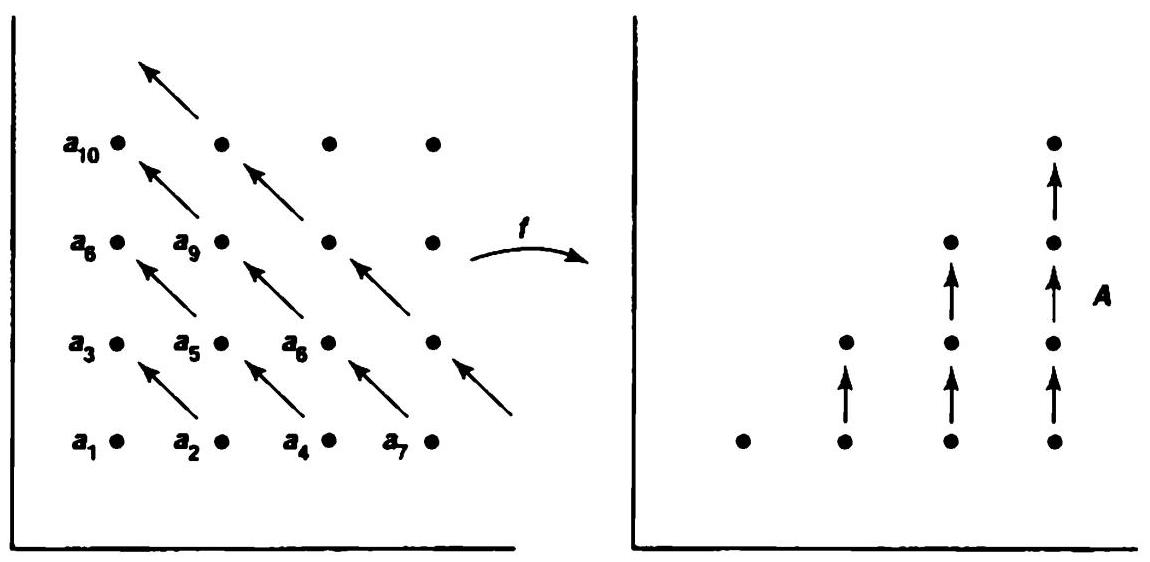
\includegraphics[width=1.0\textwidth]{images/7.1.jpg}
\end{center}
\hspace*{3em} 

Figure 7.1

\begin{definition} A set is said to be countable if it is either finite or countably infinite. A set that is not countable is said to be uncountable.
\end{definition}

There is a very useful criterion for showing that a set is countable. It is the following:

\begin{theorem} Let \(B\) be a nonempty set. Then the following are equivalent:

(1) \(B\) is countable

(2) There is a surjective function \(f : {\mathbb{Z}}_{ + } \rightarrow  B\) .

(3) There is an injective function \(g : B \rightarrow  {\mathbb{Z}}_{ + }\) .

\begin{proof}(1) \(\Rightarrow\) (2). Suppose that \(B\) is countable. If \(B\) is countably infinite, there is a bijection \(f : {\mathbb{Z}}_{ + } \rightarrow  B\) by definition, and we are through. If \(B\) is finite, there is a bijection \(h : \{ 1,\ldots ,n\}  \rightarrow  B\) for some \(n \geq  1\) . (Recall that \(B \neq  \varnothing\) .) We can extend \(h\) to a surjection \(f : {\mathbb{Z}}_{ + } \rightarrow  B\) by defining
\[
f\left( i\right)  = \left\{  \begin{array}{ll} h\left( i\right) & \text{ for }1 \leq  i \leq  n, \\  h\left( 1\right) & \text{ for }i > n. \end{array}\right.
\]

\(\left( 2\right)  \Rightarrow  \left( 3\right)\) . Let \(f : {\mathbb{Z}}_{ + } \rightarrow  B\) be a surjection. Define \(g : B \rightarrow  {\mathbb{Z}}_{ + }\) by the equation

\[
g\left( b\right)  = \text{ smallest element of }{f}^{-1}\left( {\{ b\} }\right) .
\]

Because \(f\) is surjective, \({f}^{-1}\left( {\{ b\} }\right)\) is nonempty; thus \(g\) is well defined. The map \(g\) is injective, for if \(b \neq  {b}^{\prime }\) , the sets \({f}^{-1}\left( {\{ b\} }\right)\) and \({f}^{-1}\left( \left\{  {b}^{\prime }\right\}  \right)\) are disjoint, so their smallest elements are different.

\(\left( 3\right)  \Rightarrow  \left( 1\right)\) . Let \(g : B \rightarrow  {\mathbb{Z}}_{ + }\) be an injection; we wish to prove \(B\) is countable. By changing the range of \(g\) , we can obtain a bijection of \(B\) with a subset of \({\mathbb{Z}}_{ + }\) . Thus to prove our result, it suffices to show that every subset of \({\mathbb{Z}}_{ + }\) is countable. So let \(C\) be a subset of \({\mathbb{Z}}_{ + }\) .

If \(C\) is finite, it is countable by definition. So what we need to prove is that every infinite subset \(C\) of \({\mathbb{Z}}_{ + }\) is countably infinite. This statement is certainly plausible. For the elements of \(C\) can easily be arranged in an infinite sequence; one simply takes the set \({\mathbb{Z}}_{ + }\) in its usual order and ``erases'' all the elements of \({\mathbb{Z}}_{ + }\) that are not in \(C\) !

The plausibility of this argument may make one overlook its informality. Providing a formal proof requires a certain amount of care. We state this result as a separate lemma, which follows.
\end{proof}
\section*{Lemma 7.2. If \(C\) is an infinite subset of \({\mathbb{Z}}_{ + }\) , then \(C\) is countably infinite.}

\begin{proof}We define a bijection \(h : {\mathbb{Z}}_{ + } \rightarrow  C\) . We proceed by induction. Define \(h\left( 1\right)\) to be the smallest element of \(C\) ; it exists because every nonempty subset \(C\) of \({\mathbb{Z}}_{ + }\) has a smallest element. Then assuming that \(h\left( 1\right) ,\ldots ,h\left( {n - 1}\right)\) are defined, define
\[
h\left( n\right)  = \text{ smallest element of }\left\lbrack  {C - h\left( {\{ 1,\ldots ,n - 1\} }\right) }\right\rbrack  .
\]

The set \(C - h\left( {\{ 1,\ldots ,n - 1\} }\right)\) is not empty; for if it were empty, then \(h : \{ 1,\ldots ,n -\)  \(1\}  \rightarrow  C\) would be surjective, so that \(C\) would be finite (by Corollary 6.7). Thus \(h\left( n\right)\) is well defined. By induction, we have defined \(h\left( n\right)\) for all \(n \in  {\mathbb{Z}}_{ + }\) .

To show that \(h\) is injective is easy. Given \(m < n\) , note that \(h\left( m\right)\) belongs to the set \(h\left( {\{ 1,\ldots ,n - 1\} }\right)\) , whereas \(h\left( n\right)\) , by definition, does not. Hence \(h\left( n\right)  \neq  h\left( m\right)\) .

To show that \(h\) is surjective, let \(c\) be any element of \(C\) ; we show that \(c\) lies in the image set of \(h\) . First note that \(h\left( {\mathbb{Z}}_{ + }\right)\) cannot be contained in the finite set \(\{ 1,\ldots ,c\}\) , because \(h\left( {\mathbb{Z}}_{ + }\right)\) is infinite (since \(h\) is injective). Therefore, there is an \(n\) in \({\mathbb{Z}}_{ + }\) , such that \(h\left( n\right)  > c\) . Let \(m\) be the smallest element of \({\mathbb{Z}}_{ + }\) , such that \(h\left( m\right)  \geq  c\) . Then for all \(i < m\) , we must have \(h\left( i\right)  < c\) . Thus, \(c\) does not belong to the set \(h\left( {\{ 1,\ldots ,m - 1\} }\right)\) . Since \(h\left( m\right)\) is defined as the smallest element of the set \(C - h\left( {\{ 1,\ldots ,m - 1\} }\right)\) , we must have \(h\left( m\right)  \leq  c\) . Putting the two inequalities together, we have \(h\left( m\right)  = c\) , as desired.

There is a point in the preceding proof where we stretched the principles of logic a bit. It occurred at the point where we said that ``using the induction principle'' we had defined the function \(h\) for all positive integers \(n\) . You may have seen arguments like this used before, with no questions raised concerning their legitimacy. We have already used such an argument ourselves, in the exercises of \(§4\) , when we defined \({a}^{n}\) .

But there is a problem here. After all, the induction principle states only that if \(A\) is an inductive set of positive integers, then \(A = {\mathbb{Z}}_{ + }\) . To use the principle to prove a theorem ``by induction,'' one begins the proof with the statement ``Let \(A\) be the set of all positive integers \(n\) for which the theorem is true,'' and then one goes ahead to prove that \(A\) is inductive, so that \(A\) must be all of \({\mathbb{Z}}_{ + }\) .

In the preceding theorem, however, we were not really proving a theorem by induction, but defining something by induction. How then should we start the proof? Can we start by saying,''Let \(A\) be the set of all integers \(n\) for which the function \(h\) is defined''? But that’s silly; the symbol \(h\) has no meaning at the outset of the proof. It only takes on meaning in the course of the proof. So something more is needed.

What is needed is another principle, which we call the principle of \idx{Recursive definition, principle} recursive definition. In the proof of the preceding theorem, we wished to assert the following:

Given the infinite subset \(C\) of \({\mathbb{Z}}_{ + }\) , there is a unique function \(h : {\mathbb{Z}}_{ + } \rightarrow  C\) satisfying the formula:

(*)
\[
h\left( 1\right)  = \text{ smallest element of }C\text{ , }
\]

\[
h\left( i\right)  = \text{ smallest element of }\left\lbrack  {C - h\left( {\{ 1,\ldots ,i - 1\} }\right) }\right\rbrack  \;\text{ for all }i > 1\text{ . }
\]

The formula \(\left( *\right)\) is called a recursion formula for \(h\) ; it defines the function \(h\) in terms of itself. A definition given by such a formula is called a recursive definition.

Now one can get into logical difficulties when one tries to define something recursively. Not all recursive formulas make sense. The recursive formula

\[
h\left( i\right)  = \text{ smallest element of }\left\lbrack  {C - h\left( {\{ 1,\ldots ,i + 1\} }\right) }\right\rbrack  .
\]

for example, is self-contradictory; although \(h\left( i\right)\) necessarily is an element of the set \(h\left( {\{ 1,\ldots ,i + 1\} }\right)\) , this formula says that it does not belong to the set. Another example is the classic \idx{Russell's paradox} paradox:

Let the \idx{Barber of Seville paradox} barber of Seville shave every man of Seville who does not shave himself. Who shall shave the barber?

In this statement, the barber appears twice, once in the phrase ``the barber of Seville'' and once as an element of the set ``men of Seville'', this definition of whom the barber shall shave is a recursive one. It also happens to be self-contradictory.

Some recursive formulas do make sense, however Specifically, one has the following principle:

Principle of recursive definition. Let \(A\) be a set. Given a formula that defines \(h\left( 1\right)\) as a unique element of \(A\) , and for \(i > 1\) defines \(h\left( i\right)\) uniquely as an element of \(A\) in terms of the values of \(h\) for positive integers less than \(i\) , this formula determines a unique function \(h : {\mathbb{Z}}_{ + } \rightarrow  A\) .

This principle is the one we actually used in the proof of Lemma 7.2. You can simply accept it on faith if you like. It may however be proved rigorously, using the principle of induction. We shall formulate it more precisely in the next section and indicate how it is proved. Mathematicians seldom refer to this principle specifically. They are much more likely to write a proof like our proof of Lemma 7.2 above, a proof in which they invoke the ``induction principle'' to define a function when what they are really using is the principle of recursive definition. We shall avoid undue pedantry in this book by following their example.
\end{proof}
\begin{corollary} A subset of a countable set is countable.
\end{corollary}

\begin{proof}Suppose \(A \subset  B\) , where \(B\) is countable. There is an injection \(f\) of \(B\) into \({\mathbb{Z}}_{ + }\) ; the restriction of \(f\) to \(A\) is an injection of \(A\) into \({\mathbb{Z}}_{ + }\) .\end{proof}
\begin{corollary} The set \({\mathbb{Z}}_{ + } \times  {\mathbb{Z}}_{ + }\) is countably infinite.
\end{corollary}

\begin{proof}In view of Theorem 7.1, it suffices to construct an injective map \(f : {\mathbb{Z}}_{ + } \times\)  \({\mathbb{Z}}_{ + } \rightarrow  {\mathbb{Z}}_{ + }\) . We define \(f\) by the equation
\[
f\left( {n,m}\right)  = {2}^{n}{3}^{m}.
\]

It is easy to check that \(f\) is injective. For suppose that \({2}^{n}{3}^{m} = {2}^{p}{3}^{q}\) . If \(n < p\) , then \({3}^{m} = {2}^{p - n}{3}^{q}\) , contradicting the fact that \({3}^{m}\) is odd for all \(m\) . Therefore, \(n = p\) . As a result, \({3}^{m} = {3}^{q}\) , Then if \(m < q\) , it follows that \(1 = {3}^{q - m}\) , another contradiction. Hence \(m = q\) .

\begin{example} The set \({\mathbb{Q}}_{ + }\) of positive rational numbers is countably infinite. For we can define a surjection \(g \cdot  {\mathbb{Z}}_{ + } \times  {\mathbb{Z}}_{ + } \rightarrow  {\mathbb{Q}}_{ + }\) by the equation

\[
g\left( {n,m}\right)  = m/n
\]

Because \({\mathbb{Z}}_{ + } \times  {\mathbb{Z}}_{ + }\) is countable, there is a surjection \(f : {\mathbb{Z}}_{ + } \rightarrow  {\mathbb{Z}}_{ + } \times  {\mathbb{Z}}_{ + }\) . Then the composite \(g \circ  f.{\mathbb{Z}}_{ + } \rightarrow  {\mathbb{Q}}_{ + }\) is a surjection, so that \({\mathbb{Q}}_{ + }\) is countable. And, of course, \({\mathbb{Q}}_{ + }\) is infinite because it contains \({\mathbb{Z}}_{ + }\) .
\end{example}

We leave it as an exercise to show the set \(\mathbb{Q}\) of all rational numbers is countably infinite.
\end{proof}
\section*{Theorem 7.5. A countable union of countable sets is countable.}

\begin{proof}Let \({\left\{  {A}_{n}\right\}  }_{n \in  J}\) be an indexed family of countable sets, where the index set \(J\) is either \(\{ 1,\ldots ,N\}\) or \({\mathbb{Z}}_{ + }\) . Assume that each set \({A}_{n}\) is nonempty, for convenience; this assumption does not change anything.
Because each \({A}_{n}\) is countable, we can choose, for each \(n\) , a surjective function \({f}_{n} : {\mathbb{Z}}_{ + } \rightarrow  {A}_{n}\) . Similarly, we can choose a surjective function \(g : {\mathbb{Z}}_{ + } \rightarrow  J\) . Now define

\[
h : {\mathbb{Z}}_{ + } \times  {\mathbb{Z}}_{ + } \rightarrow  \mathop{\bigcup }\limits_{{n \in  J}}{A}_{n}
\]

by the equation

\[
h\left( {k,m}\right)  = {f}_{g\left( k\right) }\left( m\right) .
\]

It is easy to check that \(h\) is surjective. Since \({\mathbb{Z}}_{ + } \times  {\mathbb{Z}}_{ + }\) is in bijective correspondence with \({\mathbb{Z}}_{ + }\) , the \idx{countability} of the union follows from Theorem 7.1.
\end{proof}
\section*{Theorem 7.6. A finite product of countable sets is countable.}

\begin{proof}First let us show that the product of two countable sets \(A\) and \(B\) is countable. The result is trivial if \(A\) or \(B\) is empty. Otherwise, choose surjective functions \(f\) : \({\mathbb{Z}}_{ + } \rightarrow  A\) and \(g : {\mathbb{Z}}_{ + } \rightarrow  B\) . Then the function \(h : {\mathbb{Z}}_{ + } \times  {\mathbb{Z}}_{ + } \rightarrow  A \times  B\) defined by the equation \(h\left( {n,m}\right)  = \left( {f\left( n\right) ,g\left( m\right) }\right)\) is surjective, so that \(A \times  B\) is countable.
In general, we proceed by induction. Assuming that \({A}_{1} \times  \cdots  \times  {A}_{n - 1}\) is countable if each \({A}_{i}\) is countable, we prove the same thing for the product \({A}_{1} \times  \cdots  \times  {A}_{n}\) . First, note that there is a bijective correspondence

\[
g : {A}_{1} \times  \cdots  \times  {A}_{n} \rightarrow  \left( {{A}_{1} \times  \cdots  \times  {A}_{n - 1}}\right)  \times  {A}_{n}
\]

defined by the equation

\[
g\left( {{x}_{1},\ldots ,{x}_{n}}\right)  = \left( {\left( {{x}_{1},\ldots ,{x}_{n - 1}}\right) ,{x}_{n}}\right) .
\]

Because the set \({A}_{1} \times  \cdots  \times  {A}_{n - 1}\) is countable by the induction assumption and \({A}_{n}\) is countable by hypothesis, the product of these two sets is countable, as proved in the preceding paragraph. We conclude that \({A}_{1} \times  \cdots  \times  {A}_{n}\) is countable as well.

It is very tempting to assert that countable products of countable sets should be countable; but this assertion is in fact not true:
\end{proof}
\end{theorem}

\begin{theorem} Let \(X\) denote the two element set \(\{ 0,1\}\) . Then the set \({X}^{\omega }\) is uncountable.
\end{theorem}

\begin{proof}We show that, given any function
\[
g : {\mathbb{Z}}_{ + } \rightarrow  {X}^{\omega }
\]

\(g\) is not surjective. For this purpose, let us denote \(g\left( n\right)\) as follows :

\[
g\left( n\right)  = \left( {{x}_{n1},{x}_{n2},{x}_{n3},\ldots {x}_{nm},\ldots }\right) ,
\]

where each \({x}_{ij}\) is either 0 or 1 . Then we define an element \(\mathbf{y} = \left( {{y}_{1},{y}_{2},\ldots ,{y}_{n},\ldots }\right)\) of \({X}^{\omega }\) by letting

\[
{y}_{n} = \left\{  \begin{array}{ll} 0 & \text{ if }{x}_{nn} = 1, \\  1 & \text{ if }{x}_{nn} = 0. \end{array}\right.
\]

(If we write the numbers \({x}_{n1}\) in a rectangular array, the particular elements \({x}_{nn}\) appear as the diagonal entries in this array; we choose \(\mathbf{y}\) so that its \(n\) th coordinate differs from the diagonal entry \({x}_{nn}\) .)

Now \(\mathbf{y}\) is an element of \({X}^{\omega }\) , and \(\mathbf{y}\) does not lie in the image of \(g\) ; given \(n\) , the point \(g\left( n\right)\) and the point \(y\) differ in at least one coordinate, namely, the \(n\) th. Thus, \(g\) is not surjective.

The cartesian product \(\{ 0,1{\} }^{\omega }\) is one example of an uncountable set. Another is the set \(\mathcal{P}\left( {\mathbb{Z}}_{ + }\right)\) , as the following theorem implies:
\end{proof}
\begin{theorem} Let \(A\) be a set. There is no injective map \(f : \mathcal{P}\left( A\right)  \rightarrow  A\) , and there is no surjective map \(g : A \rightarrow  \mathcal{P}\left( A\right)\) .
\end{theorem}

\begin{proof}In general, if \(B\) is a nonempty set, the existence of an injective map \(f : B \rightarrow\)  \(C\) implies the existence of a surjective map \(g : C \rightarrow  B\) ; one defines \(g\left( c\right)  = {f}^{-1}\left( c\right)\) for each \(c\) in the image set of \(f\) , and defines \(g\) arbitrarily on the rest of \(C\) .
Therefore, it suffices to prove that given a map \(g : A \rightarrow  \mathcal{P}\left( A\right)\) , the map \(g\) is not surjective For each \(a \in  A\) , the image \(g\left( a\right)\) of \(a\) is a subset of \(A\) , which may or may not contain the point \(a\) itself. Let \(B\) be the subset of \(A\) consisting of all those points \(a\) such that \(g\left( a\right)\) does not contain \(a\) ;

\[
B = \{ a \mid  a \in  A - g\left( a\right) \} .
\]

Now, \(B\) may be empty, or it may be all of \(A\) , but that does not matter. We assert that \(B\) is a subset of \(A\) that does not lie in the image of \(g\) . For suppose that \(B = g\left( {a}_{0}\right)\) for some \({a}_{0} \in  A\) . We ask the question: Does \({a}_{0}\) belong to \(B\) or not? By definition of \(B\) ,

\[
{a}_{0} \in  B \Leftrightarrow  {a}_{0} \in  A - g\left( {a}_{0}\right)  \Leftrightarrow  {a}_{0} \in  A - B.
\]

In either case, we have a contradiction.

Now we have proved the existence of uncountable sets. But we have not yet mentioned the most familiar uncountable set of all-the set of real numbers. You have probably seen the uncountability of \(\mathbb{R}\) demonstrated already. If one assumes that every real number can be represented uniquely by an infinite decimal (with the proviso that a representation ending in an infinite string of 9 's is forbidden), then the uncountability of the reals can be proved by a variant of the diagonal procedure used in the proof of Theorem 7.7. But this proof is in some ways not very satisfying. One reason is that the infinite decimal representation of a real number is not at all an elementary consequence of the axioms but requires a good deal of labor to prove. Another reason is that the uncountability of \(\mathbb{R}\) does not, in fact, depend on the infinite decimal expansion of \(\mathbb{R}\) or indeed on any of the algebraic properties of \(\mathbb{R}\) ; it depends on only the order properties of \(\mathbb{R}\) . We shall demonstrate the uncountability of \(\mathbb{R}\) , using only its order properties, in a later chapter.
\end{proof}
\section*{Exercises}

1. Show that \(\mathbb{Q}\) is countably infinite.

2. Show that the maps \(f\) and \(g\) of Examples 1 and 2 are bijections.

3. Let \(X\) be the two-element set \(\{ 0,1\}\) . Show there is a bijective correspondence between the set \(\mathcal{P}\left( {\mathbb{Z}}_{ + }\right)\) and the cartesian product \({X}^{\omega }\) .

4. (a) A real number \(x\) is said to be algebraic (over the rationals) if it satisfies some polynomial equation of positive degree

\[
{x}^{n} + {a}_{n - 1}{x}^{n - 1} + \cdots  + {a}_{1}x + {a}_{0} = 0
\]

with rational coefficients \({a}_{i}\) . Assuming that each polynomial equation has only finitely many roots, show that the set of \idx{algebraic number}s is countable.

(b) A real number is said to be transcendental if it is not algebraic. Assuming the reals are uncountable, show that the \idx{transcendental number}s are uncountable. (It is a somewhat surprising fact that only two transcendental numbers are familiar to us: \(e\) and \(\pi\) . Even proving these two numbers transcendental is highly nontrivial.)

5. Determine, for each of the following sets, whether or not it is countable. Justify your answers.

(a) The set \(A\) of all functions \(f : \{ 0,1\}  \rightarrow  {\mathbb{Z}}_{ + }\) .

(b) The set \({B}_{n}\) of all functions \(f : \{ 1,\ldots ,n\}  \rightarrow  {\mathbb{Z}}_{ + }\) .

(c) The set \(C = \mathop{\bigcup }\limits_{{n \in  {\mathbf{Z}}_{ + }}}{B}_{n}\) .

(d) The set \(D\) of all functions \(f : {\mathbb{Z}}_{ + } \rightarrow  {\mathbb{Z}}_{ + }\) .

(e) The set \(E\) of all functions \(f : {\mathbb{Z}}_{ + } \rightarrow  \{ 0,1\}\) .

(f) The set \(F\) of all functions \(f : {\mathbb{Z}}_{ + } \rightarrow  \{ 0,1\}\) that are ``\idx{eventually zero}.'' [We say that \(f\) is eventually zero if there is a positive integer \(N\) such that \(f\left( n\right)  = 0\) for all \(n \geq  N\) ]

(g) The set \(G\) of all functions \(f : {\mathbb{Z}}_{ + } \rightarrow  {\mathbb{Z}}_{ + }\) that are eventually 1 .

(h) The set \(H\) of all functions \(f : {\mathbb{Z}}_{ + } \rightarrow  {\mathbb{Z}}_{ + }\) that are eventually constant.

(i) The set \(I\) of all two-element subsets of \({\mathbb{Z}}_{ + }\) .

(j) The set \(J\) of all finite subsets of \({\mathbb{Z}}_{ + }\) .

6. We say that two sets \(A\) and \(B\) \idx{have the same cardinality} if there is a bijection of \(A\) with \(B\) .

(a) Show that if \(B \subset  A\) and if there is an injection

\[
f : A \rightarrow  B,
\]

then \(A\) and \(B\) have the same cardinality. [Hint: Define \({A}_{1} = A,{B}_{1} = B\) . and for \(n > 1,{A}_{n} = f\left( {A}_{n - 1}\right)\) and \({B}_{n} = f\left( {B}_{n - 1}\right)\) . (Recursive definition again!) Note that \({A}_{1} \supset  {B}_{1} \supset  {A}_{2} \supset  {B}_{2} \supset  {A}_{3} \supset  \cdots\) . Define a bijection \(h : A \rightarrow  B\) by the rule

\[
h\left( x\right)  = \left\{  \begin{array}{ll} f\left( x\right) & \text{ if }x \in  {A}_{n} - {B}_{n}\text{ for some }n, \\  x & \text{ otherwise.] } \end{array}\right.
\]

(b) Theorem (\idx{Schroeder-Bernstein theorem}). If there are injections \(f : A \rightarrow\)  \(C\) and \(g : C \rightarrow  A\) , then \(A\) and \(C\) have the same cardinality.

7. Show that the sets \(D\) and \(E\) of Exercise 5 have the same cardinality.

8. Let \(X\) denote the two-element set \(\{ 0,1\}\) ; let \(\mathcal{B}\) be the set of countable subsets of \({X}^{\omega }\) . Show that \({X}^{\omega }\) and \(\mathcal{B}\) have the same cardinality.

9. (a) The formula

\[
h\left( 1\right)  = 1,
\]

(*)
\[
h\left( 2\right)  = 2\text{ , }
\]

\[
h\left( n\right)  = {\left\lbrack  h\left( n + 1\right) \right\rbrack  }^{2} - {\left\lbrack  h\left( n - 1\right) \right\rbrack  }^{2}\;\text{ for }n \geq  2
\]

is not one to which the principle of recursive definition applies. Show that nevertheless there does exist a function \(h : {\mathbb{Z}}_{ + } \rightarrow  \mathbb{R}\) satisfying this formula. [Hint: Reformulate (*) so that the principle will apply and require \(h\) to be positive.]

(b) Show that the formula (*) of part (a) does not determine \(h\) uniquely. [Hint: If \(h\) is a positive function satisfying \(\left( *\right)\) , let \(f\left( i\right)  = h\left( i\right)\) for \(i \neq  3\) , and let \(f\left( 3\right)  =  - h\left( 3\right)\) .]

(c) Show that there is no function \(h : {\mathbb{Z}}_{ + } \rightarrow  \mathbb{R}\) satisfying the formula

\[
h\left( 1\right)  = 1,
\]

\[
h\left( 2\right)  = 2,
\]

\[
h\left( n\right)  = {\left\lbrack  h\left( n + 1\right) \right\rbrack  }^{2} + {\left\lbrack  h\left( n - 1\right) \right\rbrack  }^{2}\;\text{ for }n \geq  2.
\]

\section*{*§ 8 The Principle of Recursive Definition}

Before considering the general form of the principle of recursive definition, let us first prove it in a specific case, that of Lemma 7.2. That should make the underlying idea of the proof much clearer when we consider the general case.

So, given the infinite subset \(C\) of \({\mathbb{Z}}_{ + }\) , let us consider the following recursion formula for a function \(h : {\mathbb{Z}}_{ + } \rightarrow  C\) :

(*)
\[
h\left( 1\right)  = \text{ smallest element of }C\text{ , }
\]

\[
h\left( i\right)  = \text{ smallest element of }\left\lbrack  {C - h\left( {\{ 1,\ldots ,i - 1\} }\right) }\right\rbrack  \;\text{ for }i > 1\text{ . }
\]

We shall prove that there exists a unique function \(h : {\mathbb{Z}}_{ + } \rightarrow  C\) satisfying this recursion formula.

The first step is to prove that there exist functions defined on sections \(\{ 1,\ldots ,n\}\) of \({\mathbb{Z}}_{ + }\) that satisfy \(\left( *\right)\) :

\begin{lemma} Given \(n \in  {\mathbb{Z}}_{ + }\) , there exists a function

\[
f : \{ 1,\ldots ,n\}  \rightarrow  C
\]

that satisfies \(\left( *\right)\) for all \(i\) in its domain.
\end{lemma}
\begin{proof} The point of this lemma is that it is a statement that depends on \(n\) ; therefore, it is capable of being proved by induction. Let \(A\) be the set of all \(n\) for which the lemma holds. We show that \(A\) is inductive. It then follows that \(A = {\mathbb{Z}}_{ + }\) .

The lemma is true for \(n = 1\) , since the function \(f : \{ 1\}  \rightarrow  C\) defined by the equation

\[
f\left( 1\right)  = \text{ smallest element of }C
\]

satisfies (*).

Supposing the lemma to be true for \(n - 1\) , we prove it true for \(n\) . By hypothesis, there is a function \({f}^{\prime } : \{ 1,\ldots ,n - 1\}  \rightarrow  C\) satisfying \(\left( *\right)\) for all \(i\) in its domain. Define \(f : \{ 1,\ldots ,n\}  \rightarrow  C\) by the equations

\[
f\left( i\right)  = {f}^{\prime }\left( i\right) \;\text{ for }i \in  \{ 1,\ldots ,n - 1\} ,
\]

\[
f\left( n\right)  = \text{ smallest element of }\left\lbrack  {C - {f}^{\prime }\left( {\{ 1,\ldots ,n - 1\} }\right) }\right\rbrack  .
\]

Since \(C\) is infinite, \({f}^{\prime }\) is not surjective; hence the set \(C - {f}^{\prime }\left( {\{ 1,\ldots ,n - 1\} }\right)\) is not empty, and \(f\left( n\right)\) is well defined. Note that this definition is an acceptable one; it does not define \(f\) in terms of itself but in terms of the given function \({f}^{\prime }\) .

It is easy to check that \(f\) satisfies \(\left( *\right)\) for all \(i\) in its domain. The function \(f\) satisfies \(\left( *\right)\) for \(i \leq  n - 1\) because it equals \({f}^{\prime }\) there. And \(f\) satisfies \(\left( *\right)\) for \(i = n\) because, by definition,

\[
f\left( n\right)  = \text{ smallest element of }\left\lbrack  {C - {f}^{\prime }\left( {\{ 1,\ldots ,n - 1\} }\right) }\right\rbrack
\]

and \({f}^{\prime }\left( {\{ 1,\ldots ,n - 1\} }\right)  = f\left( {\{ 1,\ldots ,n - 1\} }\right)\) .
\end{proof}

\begin{lemma} Suppose that \(f.\{ 1,\ldots ,n\}  \rightarrow  C\) and \(g : \{ 1,\ldots ,m\}  \rightarrow  C\) both satisfy \(\left( *\right)\) for all \(i\) in their respective domains. Then \(f\left( i\right)  = g\left( i\right)\) for all \(i\) in both domains.
\end{lemma}

\begin{proof}Suppose not. Let \(i\) be the smallest integer for which \(f\left( i\right)  \neq  g\left( i\right)\) . The integer \(i\) is not 1, because
\[
f\left( 1\right)  = \text{ smallest element of }C = g\left( 1\right) ,
\]

by \(\left( *\right)\) . Now for all \(j < i\) , we have \(f\left( j\right)  = g\left( j\right)\) . Because \(f\) and \(g\) satisfy \(\left( *\right)\) ,

\[
f\left( i\right)  = \text{ smallest element of }\lbrack C - f\left( {\{ 1,\ldots ,i - 1\} }\right) \} ,
\]

\[
g\left( i\right)  = \text{ smallest element of }\left\lbrack  {C - g\left( {\{ 1,\ldots ,i - 1\} }\right) }\right\rbrack  \text{ . }
\]

Since \(f\left( {\{ 1,\ldots ,i - 1\} }\right)  = g\left( {\{ 1,\ldots ,i - 1\} }\right)\) , we have \(f\left( i\right)  = g\left( i\right)\) , contrary to the choice of \(i\) .
\end{proof}
\begin{theorem} There exists a unique function \(h : {\mathbb{Z}}_{ + } \rightarrow  C\) satisfying \(\left( *\right)\) for all \(i \in  {\mathbb{Z}}_{ + }\) .
\end{theorem}

\begin{proof}By Lemma 8.1, there exists for each \(n\) a function that maps \(\{ 1,\ldots ,n\}\) into \(C\) and satisfies \(\left( *\right)\) for all \(i\) in its domain. Given \(n\) , Lemma 8.2 shows that this function is unique; two such functions having the same domain must be equal. Let \({f}_{n}\) : \(\{ 1,\ldots ,n\}  \rightarrow  C\) denote this unique function.
Now comes the crucial step. We define a function \(h : {\mathbb{Z}}_{ + } \rightarrow  C\) by defining its rule to be the union \(U\) of the rules of the functions \({f}_{n}\) . The rule for \({f}_{n}\) is a subset of \(\{ 1,\ldots ,n\}  \times  C\) ; therefore, \(U\) is a subset of \({\mathbb{Z}}_{ + } \times  C\) . We must show that \(U\) is the rule for a function \(h : {\mathbb{Z}}_{ + } \rightarrow  C\)

That is, we must show that each element \(i\) of \({\mathbb{Z}}_{ + }\) appears as the first coordinate of exactly one element of \(U\) . This is easy. The integer \(i\) lies in the domain of \({f}_{n}\) if and only if \(n > i\) . Therefore, the set of elements of \(U\) of which \(i\) is the first coordinate is precisely the set of all pairs of the form \(\left( {i,{f}_{n}\left( i\right) }\right)\) , for \(n \geq  i\) . Now Lemma 8.2 tells us that \({f}_{n}\left( i\right)  = {f}_{m}\left( i\right)\) if \(n,m \geq  i\) . Therefore, all these elements of \(U\) are equal; that is, there is only one element of \(U\) that has \(i\) as its first coordinate.

To show that \(h\) satisfies \(\left( *\right)\) is also easy; it is a consequence of the following facts:

\[
h\left( i\right)  = {f}_{n}\left( i\right) \;\text{ for }i \leq  n,
\]

\[
{f}_{n}\text{ satisfies }\left( *\right) \text{ for all }i\text{ in its domain. }
\]

The proof of uniqueness is a copy of the proof of Lemma 8.2.

Now we formulate the general principle of recursive definition. There are no new ideas involved in its proof, so we leave it as an exercise.
\end{proof}
\begin{theorem}[Principle of recursive definition] Let \(A\) be a set; let \({a}_{0}\) be an element of \(A\) . Suppose \(\rho\) is a function that assigns, to each function \(f\) mapping a nonempty section of the positive integers into \(A\) , an element of \(A\) . Then there exists a unique function

\[
h : {\mathbb{Z}}_{ + } \rightarrow  A
\]

such that

(*)
\[
h\left( 1\right)  = {a}_{0},
\]

\[
h\left( i\right)  = \rho \left( {h|\{ 1,\ldots ,i - 1\} }\right) \;\text{ for }i > 1.
\]

The formula \(\left( *\right)\) is called a recursion formula for \(h\) . It specifies \(h\left( 1\right)\) , and it expresses the value of \(h\) at \(i > 1\) in terms of the values of \(h\) for positive integers less than \(i\) .

\begin{example} Let us show that Theorem 8.3 is a special case of this theorem. Given the infinite subset \(C\) of \({\mathbb{Z}}_{ + }\) , let \({a}_{0}\) be the smallest element of \(C\) , and define \(\rho\) by the equation

\[
\rho \left( f\right)  = \text{ smallest element of }\left\lbrack  {C - \left( {\text{ image set of }f}\right) }\right\rbrack  \text{ . }
\]

Because \(C\) is infinite and \(f\) is a function mapping a finite set into \(C\) , the image set of \(f\) is not all of \(C\) , therefore, \(\rho\) is well defined. By Theorem 8.4 there exists a function \(h \cdot  {\mathbb{Z}}_{ + } \rightarrow\)  \(C\) such that \(h\left( 1\right)  = {a}_{0}\) , and for \(i > 1\) ,

\[
h\left( i\right)  = \rho \left( {h|\{ 1,\ldots ,i - 1\} }\right)
\]

\[
= \text{ smallest element of }\left\lbrack  {C - \left( {\text{ image set of }h \mid  \{ 1,\ldots ,i - 1\} }\right) }\right\rbrack
\]

\[
= \text{ smallest element of }\left\lbrack  {C - h\left( {\{ 1\ldots ,i - 1\} }\right) }\right\rbrack  \text{ , }
\]

as desired.
\end{example}

\begin{example} Given \(a \in  \mathbb{R}\) , we ``defined'' \({a}^{n}\) , in the exercises of \(\$ 4\) , by the recursion formula

\[
{a}^{1} = a
\]

\[
{a}^{n} = {a}^{n - 1} \cdot  a
\]

We wish to apply Theorem 8.4 to define a function \(h : {\mathbb{Z}}_{ + } \rightarrow  \mathbb{R}\) ngorously such that \(h\left( n\right)  = {a}^{n}\) . To apply this theorem, let \({a}_{0}\) denote the element \(a\) of \(\mathbb{R}\) , and define \(\rho\) by the equation \(\rho \left( f\right)  = f\left( m\right)  \cdot  a\) , where \(f.\{ 1,\ldots ,m\}  \rightarrow  \mathbb{R}\) Then there exists a unique function \(h : {\mathbb{Z}}_{ + } \rightarrow  \mathbb{R}\) such that

\[
h\left( 1\right)  = {a}_{0},
\]

\[
h\left( i\right)  = \rho \left( {h|\{ 1,\ldots ,i - 1\} }\right) \;\text{ for }i > 1.
\]

This means that \(h\left( 1\right)  = a\) , and \(h\left( i\right)  = h\left( {i - 1}\right)  \cdot  a\) for \(i > 1\) . If we denote \(h\left( i\right)\) by \({a}^{i}\) , we have

\[
{a}^{1} = a,
\]

\[
{a}^{l} = {a}^{l - 1} \cdot  a
\]

as desired.
\end{example}

\section*{Exercises}

1. Let \(\left( {{b}_{1},{b}_{2},\ldots }\right)\) be an infinite sequence of real numbers. The sum \(\mathop{\sum }\limits_{{k = 1}}^{n}{b}_{k}\) is defined by induction as follows :

\[
\mathop{\sum }\limits_{{k = 1}}^{n}{b}_{k} = {b}_{1}\;\text{ for }n = 1,
\]

\[
\mathop{\sum }\limits_{{k = 1}}^{n}{b}_{k} = \left( {\mathop{\sum }\limits_{{k = 1}}^{{n - 1}}{b}_{k}}\right)  + {b}_{n}\;\text{ for }n > 1.
\]

Let \(A\) be the set of real numbers; choose \(\rho\) so that Theorem 8.4 applies to define this sum rigorously. We sometimes denote the sum \(\mathop{\sum }\limits_{{k = 1}}^{n}{b}_{k}\) by the symbol \({b}_{1} + {b}_{2} + \cdots  + {b}_{n}\) .

2. Let \(\left( {{b}_{1},{b}_{2},\ldots }\right)\) be an infinite sequence of real numbers. We define the product \(\mathop{\prod }\limits_{{k = 1}}^{n}{b}_{k}\) by the equations

\[
\mathop{\prod }\limits_{{k = 1}}^{1}{b}_{k} = {b}_{1}
\]

\[
\mathop{\prod }\limits_{{k = 1}}^{n}{b}_{k} = \left( {\mathop{\prod }\limits_{{k = 1}}^{{n - 1}}{b}_{k}}\right)  \cdot  {b}_{n}\;\text{ for }n > 1.
\]

Use Theorem 8.4 to define this product rigorously. We sometimes denote the product \(\mathop{\prod }\limits_{{k = 1}}^{n}{b}_{k}\) by the symbol \({b}_{1}{b}_{2}\cdots {b}_{n}\) . 3. Obtain the definitions of \({a}^{n}\) and \(n\) ! for \(n \in  {\mathbb{Z}}_{ + }\) as special cases of Exercise 2. 4. The \idx{Fibonacci numbers} of number theory are defined recursively by the formula

\[
{\lambda }_{1} = {\lambda }_{2} = 1
\]

\[
{\lambda }_{n} = {\lambda }_{n - 1} + {\lambda }_{n - 2}\;\text{ for }n > 2.
\]

Define them rigorously by use of Theorem 8.4.

5. Show that there is a unique function \(h : {\mathbb{Z}}_{ + } \rightarrow  {\mathbb{R}}_{ + }\) satisfying the formula

\[
h\left( 1\right)  = 3,
\]

\[
h\left( i\right)  = {\left\lbrack  h\left( i - 1\right)  + 1\right\rbrack  }^{1/2}\;\text{ for }i > 1.
\]

6. (a) Show that there is no function \(h : {\mathbb{Z}}_{ + } \rightarrow  {\mathbb{R}}_{ + }\) satisfying the formula

\[
h\left( 1\right)  = 3,
\]

\[
h\left( i\right)  = {\left\lbrack  h\left( i - 1\right)  - 1\right\rbrack  }^{1/2}\;\text{ for }i > 1.
\]

Explain why this example does not violate the principle of recursive definition.

(b) Consider the recursion formula

\[
h\left( 1\right)  = 3,
\]

\[
h\left( i\right)  = \left\{  \begin{array}{ll} {\left\lbrack  h\left( i - 1\right)  - 1\right\rbrack  }^{1/2} & \text{ if }h\left( {i - 1}\right)  > 1 \\  5 & \text{ if }h\left( {i - 1}\right)  \leq  1 \end{array}\right\}  \;\text{ for }i > 1.
\]

Show that there exists a unique function \(h : {\mathbb{Z}}_{ + } \rightarrow  {\mathbb{R}}_{ + }\) satisfying this formula.

7. Prove Theorem 8.4.

8. Verify the following version of the principle of recursive definition: Let \(A\) be a set. Let \(\rho\) be a function assigning, to every function \(f\) mapping a section \({S}_{n}\) of \({\mathbb{Z}}_{ + }\) into \(A\) , an element \(\rho \left( f\right)\) of \(A\) . Then there is a unique function \(h : {\mathbb{Z}}_{ + } \rightarrow  A\) such that \(h\left( n\right)  = \rho \left( {h \mid  {S}_{n}}\right)\) for each \(n \in  {\mathbb{Z}}_{ + }\) .

\end{theorem}

\section*{§ 9 Infinite Sets and the Axiom of Choice}

We have already obtained several criteria for a set to be infinite. We know, for instance, that a set \(A\) is infinite if it has a countably infinite subset, or if there is a bijection of \(A\) with a proper subset of itself. It turns out that either of these properties is sufficient to characterize infinite sets. This we shall now prove. The proof will lead us into a discussion of a point of logic we have not yet mentioned-the \idx{axiom of choice}.

\begin{theorem} 
Let \(A\) be a set. The following statements about \(A\) are equivalent:

(1) There exists an injective function \(f : {\mathbb{Z}}_{ + } \rightarrow  A\) .

(2) There exists a bijection of \(A\) with a proper subset of itself.

(3) \(A\) is infinite.
\end{theorem}

\begin{proof}We prove the implications \(\left( 1\right)  \Rightarrow  \left( 2\right)  \Rightarrow  \left( 3\right)  \Rightarrow  \left( 1\right)\) . To prove that \(\left( 1\right)  \Rightarrow  \left( 2\right)\) , we assume there is an injective function \(f : {\mathbb{Z}}_{ + } \rightarrow  A\) . Let the image set \(f\left( {\mathbb{Z}}_{ + }\right)\) be denoted by \(B\) ; and let \(f\left( n\right)\) be denoted by \({a}_{n}\) . Because \(f\) is injective, \({a}_{n} \neq  {a}_{m}\) if \(n \neq  m\) . Define
\[
g : A \rightarrow  A - \left\{  {a}_{1}\right\}
\]

by the equations

\[
g\left( {a}_{n}\right)  = {a}_{n + 1}\;\text{ for }{a}_{n} \in  B.
\]

\[
g\left( x\right)  = x\;\text{ for }x \in  A - B.
\]

The map \(g\) is indicated schematically in Figure 9.1; one checks easily that it is a bijection.

\begin{center}
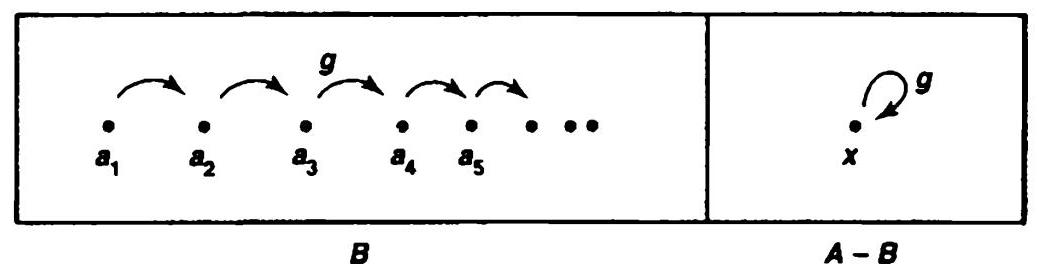
\includegraphics[width=0.9\textwidth]{images/9.1.jpg}
\end{center}
\hspace*{3em} 

Figure 9.1

The implication (2) \(\Rightarrow\) (3) is just the contrapositive of Corollary 6.3, so it has already been proved. To prove that \(\left( 3\right)  \Rightarrow  \left( 1\right)\) , we assume that \(A\) is infinite and construct ``by induction'' an injective function \(f : {\mathbb{Z}}_{ + } \rightarrow  A\) .

First, since the set \(A\) is not empty, we can choose a point \({a}_{1}\) of \(A\) ; define \(f\left( 1\right)\) to be the point so chosen.

Then, assuming that we have defined \(f\left( 1\right) ,\ldots ,f\left( {n - 1}\right)\) , we wish to define \(f\left( n\right)\) . The set \(A - f\left( {\{ 1,\ldots ,n - 1\} }\right)\) is not empty; for if it were empty, the map \(f : \{ 1,\ldots ,n -\)  \(1\}  \rightarrow  A\) would be a surjection and \(A\) would be finite. Hence, we can choose an element of the set \(A - f\left( {\{ 1,\ldots ,n - 1\} }\right)\) and define \(f\left( n\right)\) to be this element. ``Using the induction principle'', we have defined \(f\) for all \(n \in  {\mathbb{Z}}_{ + }\) .

It is easy to see that \(f\) is injective. For suppose that \(m < n\) . Then \(f\left( m\right)\) belongs to the set \(f\left( {\{ 1,\ldots ,n - 1\} }\right)\) , whereas \(f\left( n\right)\) , by definition, does not. Therefore, \(f\left( n\right)  \neq\)  \(f\left( m\right)\) .

Let us try to reformulate this ``induction'' proof more carefully, so as to make explicit our use of the principle of recursive definition.

Given the infinite set \(A\) , we attempt to define \(f : {\mathbb{Z}}_{ + } \rightarrow  A\) recursively by the formula

(*)
\[
f\left( 1\right)  = {a}_{1},
\]

\[
f\left( i\right)  = \text{ an arbitrary element of }\left\lbrack  {A - f\left( {\{ 1,\ldots ,i - 1\} }\right) }\right\rbrack  \;\text{ for }i > 1\text{ . }
\]

But this is not an acceptable recursion formula at all! For it does not define \(f\left( i\right)\) uniquely in terms of \(f \mid  \{ 1,\ldots ,i - 1\}\) .

In this respect this formula differs notably from the recursion formula we considered in proving Lemma 7.2. There we had an infinite subset \(C\) of \({\mathbb{Z}}_{ + }\) , and we defined \(h\) by the formula

\[
h\left( 1\right)  = \text{ smallest element of }C\text{ , }
\]

\[
h\left( i\right)  = \text{ smallest element of }\left\lbrack  {C - h\left( {\{ 1,\ldots ,i - 1\} }\right) }\right\rbrack  \;\text{ for }i > 1\text{ . }
\]

This formula does define \(h\left( i\right)\) uniquely in terms of \(h \mid  \{ 1,\ldots ,i - 1\}\) .

Another way of seeing that \(\left( *\right)\) is not an acceptable recursion formula is to note that if it were, the principle of recursive definition would imply that there is a unique function \(f : {\mathbb{Z}}_{ + } \rightarrow  A\) satisfying \(\left( *\right)\) . But by no stretch of the imagination does \(\left( *\right)\) specify \(f\) uniquely. In fact, this ``definition'' of \(f\) involves infinitely many arbitrary choices.

What we are saying is that the proof we have given for Theorem 9.1 is not actually a proof. Indeed, on the basis of the properties of set theory we have discussed up to now, it is not possible to prove this theorem. Something more is needed.

Previously, we described certain definite allowable methods for specifying sets:

(1) Defining a set by listing its elements, or by taking a given set \(A\) and specifying a subset \(B\) of it by giving a property that the elements of \(B\) are to satisfy.

(2) Taking unions or intersections of the elements of a given collection of sets, or taking the difference of two sets.

(3) Taking the set of all subsets of a given set.

(4) Taking cartesian products of sets.

Now the rule for the function \(f\) is really a set: a subset of \({\mathbb{Z}}_{ + } \times  A\) . Therefore, to prove the existence of the function \(f\) , we must construct the appropriate subset of \({\mathbb{Z}}_{ + } \times  A\) , using the allowed methods for forming sets. The methods already given simply are not adequate for this purpose. We need a new way of asserting the existence of a set. So, we add to the list of allowed methods of forming sets the following: Axiom of choice. Given a collection \(\mathcal{A}\) of disjoint nonempty sets, there exists a set \(C\) consisting of exactly one element from each element of \(\mathcal{A}\) ; that is, a set \(\mathbf{C}\) such that \(\mathbf{C}\) is contained in the union of the elements of \(\mathcal{A}\) , and for each \(A \in  \mathcal{A}\) , the set \(C \cap  A\) contains a single element.

The set \(C\) can be thought of as having been obtained by choosing one element from each of the sets in \(\mathcal{A}\) .

The axiom of choice certainly seems an innocent-enough assertion. And, in fact, most mathematicians today accept it as part of the set theory on which they base their mathematics. But in years past a good deal of controversy raged around this particular assertion concerning set theory, for there are theorems one can prove with its aid that some mathematicians were reluctant to accept. One such is the \idx{well-ordering theorem}, which we shall discuss shortly. For the present we shall simply use the choice axiom to clear up the difficulty we mentioned in the preceding proof. First, we prove an easy consequence of the axiom of choice:
\end{proof}
\begin{lemma}[Existence of a \idx{choice function}] Given a collection \(\mathcal{B}\) of nonempty sets (not necessarily disjoint), there exists a function

\[
c : \mathcal{B} \rightarrow  \mathop{\bigcup }\limits_{{B \in  \mathcal{B}}}B
\]

such that \(c\left( B\right)\) is an element of \(B\) , for each \(B \in  \mathcal{B}\) .

The function \(c\) is called a choice function for the collection \(\mathcal{B}\) .

The difference between this lemma and the axiom of choice is that in this lemma the sets of the collection \(\mathcal{B}\) are not required to be disjoint. For example, one can allow \(\mathcal{B}\) to be the collection of all nonempty subsets of a given set.
\end{lemma}

Proof of the lemma. Given an element \(B\) of \(\mathcal{B}\) , we define a set \({B}^{\prime }\) as follows

\[
{B}^{\prime } = \{ \left( {B,x}\right)  \mid  x \in  B\} .
\]

That is, \({B}^{\prime }\) is the collection of all ordered pairs, where the first coordinate of the ordered pair is the set \(B\) , and the second coordinate is an element of \(B\) . The set \({B}^{\prime }\) is a subset of the cartesian product

\[
\mathcal{B} \times  \mathop{\bigcup }\limits_{{B \in  \mathcal{B}}}B
\]

Because \(B\) contains at least one element \(x\) , the set \({B}^{\prime }\) contains at least the element (B, x), so it is nonempty.

Now we claim that if \({B}_{1}\) and \({B}_{2}\) are two different sets in \(\mathcal{B}\) , then the corresponding sets \({B}_{1}^{\prime }\) and \({B}_{2}^{\prime }\) are disjoint. For the typical element of \({B}_{1}^{\prime }\) is a pair of the form \(\left( {{B}_{1},{x}_{1}}\right)\) and the typical element of \({B}_{2}^{\prime }\) is a pair of the form \(\left( {{B}_{2},{x}_{2}}\right)\) . No two such elements can be equal, for their first coordinates are different. Now let us form the collection

\[
C = \left\{  {{B}^{\prime } \mid  B \in  \mathcal{B}}\right\}  \text{ ; }
\]

it is a collection of disjoint nonempty subsets of

\[
\mathcal{B} \times  \mathop{\bigcup }\limits_{{B \in  \mathcal{B}}}B
\]

By the choice axiom, there exists a set \(c\) consisting of exactly one element from each element of \(\mathcal{C}\) . Our claim is that \(c\) is the rule for the desired choice function.

In the first place, \(c\) is a subset of

\[
\mathcal{B} \times  \mathop{\bigcup }\limits_{{B \in  \mathcal{B}}}B
\]

In the second place, \(c\) contains exactly one element from each set \({B}^{\prime }\) ; therefore, for each \(B \in  \mathcal{B}\) , the set \(c\) contains exactly one ordered pair(B, x)whose first coordinate is \(B\) . Thus \(c\) is indeed the rule for a function from the collection \(\mathcal{B}\) to the set \(\mathop{\bigcup }\limits_{{B \in  \mathcal{B}}}B\) . Finally, if \(\left( {B,x}\right)  \in  c\) , then \(x\) belongs to \(B\) , so that \(c\left( B\right)  \in  B\) , as desired.

A second proof of Theorem 9.1. Using this lemma, one can make the proof of Theorem 9.1 more precise. Given the infinite set \(A\) , we wish to construct an injective function \(f : {\mathbb{Z}}_{ + } \rightarrow  A\) . Let us form the collection \(\mathcal{B}\) of all nonempty subsets of \(A\) . The lemma just proved asserts the existence of a choice function for \(\mathcal{B}\) ; that is, a function

\[
c : \mathcal{B} \rightarrow  \mathop{\bigcup }\limits_{{B \in  \mathcal{B}}}B = A
\]

such that \(c\left( B\right)  \in  B\) for each \(B \in  \mathcal{B}\) . Let us now define a function \(f : {\mathbb{Z}}_{ + } \rightarrow  A\) by the recursion formula

(*)
\[
f\left( 1\right)  = c\left( A\right)
\]

\[
f\left( i\right)  = c\left( {A - f\left( {\{ 1,\ldots ,i - 1\} }\right) }\right) \;\text{ for }i > 1.
\]

Because \(A\) is infinite, the set \(A - f\left( {\{ 1,\ldots ,i - 1\} }\right)\) is nonempty; therefore, the right side of this equation makes sense. Since this formula defines \(f\left( i\right)\) uniquely in terms of \(f \mid  \{ 1,\ldots ,i - 1\}\) , the principle of recursive definition applies. We conclude that there exists a unique function \(f : {\mathbb{Z}}_{ + } \rightarrow  A\) satisfying \(\left( *\right)\) for all \(i \in  {\mathbb{Z}}_{ + }\) . Injectivity of \(f\) follows as before.

Having emphasized that in order to construct a proof of Theorem 9.1 that is logically correct, one must make specific use of a choice function, we now backtrack and admit that in practice most mathematicians do no such thing. They go on with no qualms giving proofs like our first version, proofs that involve an infinite number of arbitrary choices. They know that they are really using the choice axiom; and they know that if it were necessary, they could put their proofs into a logically more satisfactory form by introducing a choice function specifically. But usually they do not bother.

And neither will we. You will find few further specific uses of a choice function in this book; we shall introduce a choice function only when the proof would become confusing without it. But there will be many proofs in which we make an infinite number of arbitrary choices, and in each such case we will actually be using the choice axiom implicitly.

Now we must confess that in an earlier section of this book there is a proof in which we constructed a certain function by making an infinite number of arbitrary choices. And we slipped that proof in without even mentioning the choice axiom. Our apologies for the deception. We leave it to you to ferret out which proof it was!

Let us make one final comment on the choice axiom. There are two forms of this axiom. One can be called the \idx{finite axiom of choice}; it asserts that given a finite collection \(\mathcal{A}\) of disjoint nonempty sets, there exists a set \(C\) consisting of exactly one element from each element of \(\mathcal{A}\) . One needs this weak form of the choice axiom all the time; we have used it freely in the preceding sections with no comment. No mathematician has any qualms about the finite choice axiom; it is part of everyone's set theory. Said differently, no one has qualms about a proof that involves only finitely many arbitrary choices.

The stronger form of the axiom of choice, the one that applies to an arbitrary collection \(\mathcal{A}\) of nonempty sets, is the one that is properly called ``the axiom of choice.'' When a mathematician writes, ``This proof depends on the choice axiom,'' it is invariably this stronger form of the axiom that is meant.

\section*{Exercises}

1. Define an injective map \(f : {\mathbb{Z}}_{ + } \rightarrow  {X}^{\omega }\) , where \(X\) is the two-element set \(\{ 0,1\}\) , without using the choice axiom.

2. Find if possible a choice function for each of the following collections, without using the choice axiom:

(a) The collection \(\mathcal{A}\) of nonempty subsets of \({\mathbb{Z}}_{ + }\) .

(b) The collection \(\mathcal{B}\) of nonempty subsets of \(\mathbb{Z}\) .

(c) The collection \(\mathcal{C}\) of nonempty subsets of the rational numbers \(\mathbb{Q}\) .

(d) The collection \(\mathcal{D}\) of nonempty subsets of \({X}^{\omega }\) , where \(X = \{ 0,1\}\) .

3. Suppose that \(A\) is a set and \({\left\{  {f}_{n}\right\}  }_{n \in  {\mathbf{Z}}_{ + }}\) is a given indexed family of injective functions

\[
{f}_{n} : \{ 1,\ldots ,n\}  \rightarrow  A
\]

Show that \(A\) is infinite. Can you define an injective function \(f : {\mathbb{Z}}_{ + } \rightarrow  A\) without using the choice axiom?

4. There was a theorem in \(§7\) whose proof involved an infinite number of arbitrary choices. Which one was it? Rewrite the proof so as to make explicit the use of the choice axiom. (Several of the earlier exercises have used the choice axiom also.)

5. (a) Use the choice axiom to show that if \(f : A \rightarrow  B\) is surjective, then \(f\) has a right inverse \(h \cdot  B \rightarrow  A\) .

(b) Show that if \(f : A \rightarrow  B\) is injective and \(A\) is not empty, then \(f\) has a left inverse. Is the axiom of choice needed?

6. Most of the famous paradoxes of naive set theory are associated in some way or other with the concept of the ``set of all sets.'' None of the rules we have given for forming sets allows us to consider such a set. And for good reason-the concept itself is self-contradictory. For suppose that \(\mathcal{A}\) denotes the ``set of all sets.''

(a) Show that \(\mathcal{P}\left( \mathcal{A}\right)  \subset  \mathcal{A}\) ; derive a contradiction.

(b) (Russell’s paradox.) Let \(\mathcal{B}\) be the subset of \(\mathcal{A}\) consisting of all sets that are not elements of themselves;

\[
\mathcal{B} = \{ A \mid  A \in  \mathcal{A}\text{ and }A \notin  A\} .
\]

(Of course, there may be no set \(A\) such that \(A \in  A\) ; if such is the case, then \(\mathcal{B} = \mathcal{A}\) .) Is \(\mathcal{B}\) an element of itself or not?

7. Let \(A\) and \(B\) be two nonempty sets. If there is an injection of \(B\) into \(A\) , but no injection of \(A\) into \(B\) , we say that \(A\) has \idx{greater cardinality} than \(B\) .

(a) Conclude from Theorem 9.1 that every uncountable set has greater cardinality than \({\mathbb{Z}}_{ + }\) .

(b) Show that if \(A\) has greater cardinality than \(B\) , and \(B\) has greater cardinality than \(C\) , then \(A\) has greater cardinality than \(C\) .

(c) Find a sequence \({A}_{1},{A}_{2},\ldots\) of infinite sets, such that for each \(n \in  {\mathbb{Z}}_{ + }\) , the set \({A}_{n + 1}\) has greater cardinality than \({A}_{n}\) .

(d) Find a set that for every \(n\) has cardinality greater than \({A}_{n}\) .

*8. Show that \(\mathcal{P}\left( {\mathbb{Z}}_{ + }\right)\) and \(\mathbb{R}\) have the same cardinality. [Hint: You may use the fact that every real number has a decimal expansion, which is unique if expansions that end in an infinite string of 9 ’s are forbidden.]

A famous conjecture of set theory, called the \idx{continuum hypothesis}, asserts that there exists no set having greater cardinality than \({\mathbb{Z}}_{ + }\) and lesser cardinality than \(\mathbb{R}\) . The \idx{generalized continuum hypothesis} asserts that, given the infinite set \(A\) , there is no set having greater cardinality than \(A\) and lesser cardinality than \(\mathcal{P}\left( A\right)\) . Surprisingly enough, both of these assertions have been shown to be independent of the usual axioms for set theory. For a readable expository account, see \cite{Smullyan1969}.

\section*{§ 10 Well-Ordered Sets}

One of the useful properties of the set \({\mathbb{Z}}_{ + }\) of positive integers is the fact that each of its nonempty subsets has a smallest element. Generalizing this property leads to the concept of a \idx{well-ordered set}.

\begin{definition} A set \(A\) with an order relation \(<\) is said to be well-ordered if every nonempty subset of \(A\) has a smallest element.
\end{definition}

\begin{example} Consider the set \(\{ 1,2\}  \times  {\mathbb{Z}}_{ + }\) in the dictionary ordering. Schernatically, it can be represented as one infinite sequence followed by another infinite sequence:

\[
{a}_{1},{a}_{2},{a}_{3},\ldots ;{b}_{1},{b}_{2},{b}_{3},\ldots
\]

with the understanding that each element is less than every element to the right of it. It is not difficult to see that every nonempty subset \(C\) of this ordered set has a smallest element: If \(C\) contains any one of the elements \({a}_{n}\) , we simply take the smallest element of the intersection of \(C\) with the sequence \({a}_{1},{a}_{2},\ldots\) ; while if \(C\) contains no \({a}_{n}\) , then it is a subset of the sequence \({b}_{1},{b}_{2},\ldots\) and as such has a smallest element.
\end{example}

\begin{example} Consider the set \({\mathbb{Z}}_{ + } \times  {\mathbb{Z}}_{ + }\) in the dictionary order. Schematically, it can be represented as an infinite sequence of infinite sequences. We show that it is well-ordered. Let \(X\) be a nonempty subset of \({\mathbb{Z}}_{ + } \times  {\mathbb{Z}}_{ + }\) Let \(A\) be the subset of \({\mathbb{Z}}_{ + }\) consisting of all first coordinates of elements of \(X\) Now \(A\) has a smallest element; call it \({a}_{0}\) . Then the collection

\[
\left\{  {b \mid  {a}_{0} \times  b \in  X}\right\}
\]

is a nonempty subset of \({\mathbb{Z}}_{ + }\) ; let \({b}_{0}\) be its smallest element. By definition of the dictionary order, \({a}_{0} \times  {b}_{0}\) is the smallest element of \(X\) . See Figure 10.1.

\begin{center}
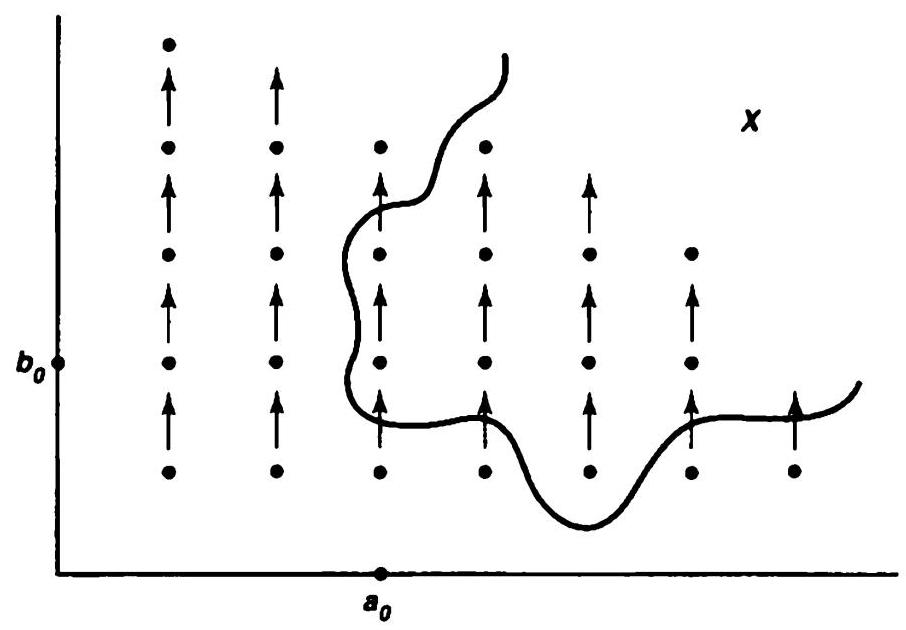
\includegraphics[width=0.8\textwidth]{images/10.1.jpg}
\end{center}
\hspace*{3em} 

Figure 10.1
\end{example}

\begin{example} The set of integers is not well-ordered in the usual order, the subset consisting of the negative integers has no smallest element. Nor is the set of real numbers in the interval \(0 \leq  x \leq  1\) well-ordered; the subset consisting of those \(x\) for which \(0 < x < 1\) has no smallest element (although it has a greatest lower bound, of course).
\end{example}

There are several ways of constructing well-ordered sets. Two of them are the following:

(1) If \(A\) is a well-ordered set, then any subset of \(A\) is well-ordered in the restricted order relation.

(2) If \(A\) and \(B\) are well-ordered sets, then \(A \times  B\) is well-ordered in the dictionary order.

The proof of (1) is trivial; the proof of (2) follows the pattern given in Example 2.

It follows that the set \({\mathbb{Z}}_{ + } \times  \left( {{\mathbb{Z}}_{ + } \times  {\mathbb{Z}}_{ + }}\right)\) is well-ordered in the dictionary order; it can be represented as an infinite sequence of infinite sequences of infinite sequences. Similarly, \({\left( {\mathbb{Z}}_{ + }\right) }^{4}\) is well-ordered in the dictionary order. And so on. But if you try to generalize to an infinite product of \({\mathbb{Z}}_{ + }\) with itself, you will run into trouble. We shall examine this situation shortly.

Now, given a set \(A\) without an order relation, it is natural to ask whether there exists an order relation for \(A\) that makes it into a well-ordered set. If \(A\) is finite, any bijection

\[
f : A \rightarrow  \{ 1,\ldots ,n\}
\]

can be used to define an order relation on \(A\) ; under this relation, \(A\) has the same order type as the ordered set \(\{ 1,\ldots ,n\}\) . In fact, every order relation on a finite set can be obtained in this way:

\begin{theorem} Every nonempty finite ordered set has the order type of a section \(\{ 1,\ldots ,n\}\) of \({\mathbb{Z}}_{ + }\) , so it is well-ordered.
\end{theorem}

\begin{proof}This was given as an exercise in \(\$ 6\) ; we prove it here. First, we show that every finite ordered set \(A\) has a largest element. If \(A\) has one element, this is trivial. Supposing it true for sets having \(n - 1\) elements, let \(A\) have \(n\) elements and let \({a}_{0} \in  A\) . Then \(A - \left\{  {a}_{0}\right\}\) has a largest element \({a}_{1}\) , and the larger of \(\left\{  {{a}_{0},{a}_{1}}\right\}\) is the largest element of \(A\) .
Second, we show there is an order-preserving bijection of \(A\) with \(\{ 1,\ldots ,n\}\) for some \(n\) . If \(A\) has one element, this fact is trivial. Suppose that it is true for sets having \(n - 1\) elements. Let \(b\) be the largest element of \(A\) . By hypothesis, there is an order-preserving bijection

\[
{f}^{\prime } : A - \{ b\}  \rightarrow  \{ 1,\ldots ,n - 1\} .
\]

Define an order-preserving bijection \(f : A \rightarrow  \{ 1,\ldots ,n\}\) by setting

\[
f\left( x\right)  = {f}^{\prime }\left( x\right) \;\text{ for }x \neq  b,
\]

\[
f\left( b\right)  = n\text{ . }
\]

Thus, a finite ordered set has only one possible order type. For an infinite set, things are quite different. The well-ordered sets

\[
{\mathbb{Z}}_{ + }\text{ , }
\]

\[
\{ 1,\ldots ,n\}  \times  {\mathbb{Z}}_{ + },
\]

\[
{\mathbb{Z}}_{ + } \times  {\mathbb{Z}}_{ + }
\]

\[
{\mathbb{Z}}_{ + } \times  \left( {{\mathbb{Z}}_{ + } \times  {\mathbb{Z}}_{ + }}\right)
\]

are all countably infinite, but they all have different order types, as you can check.

All the examples we have given of well-ordered sets are orderings of countable sets. It is natural to ask whether one can find a well-ordered uncountable set.

The obvious uncountable set to try is the countably infinite product

\[
X = {\mathbb{Z}}_{ + } \times  {\mathbb{Z}}_{ + } \times  \cdots  = {\left( {\mathbb{Z}}_{ + }\right) }^{\omega }
\]

of \({\mathbb{Z}}_{ + }\) with itself. One can generalize the dictionary order to this set in a natural way, by defining

\[
\left( {{a}_{1},{a}_{2},\ldots }\right)  < \left( {{b}_{1},{b}_{2},\ldots }\right)
\]

if for some \(n \geq  1\) ,

\[
{a}_{i} = {b}_{i},\;\text{ for }i < n\text{ and }{a}_{n} < {b}_{n}.
\]

This is, in fact, an order relation on the set \(X\) ; but unfortunately it is not a well-ordering. Consider the set \(A\) of all elements \(\mathbf{x}\) of \(X\) of the form

\[
\mathbf{x} = \left( {1,\ldots ,1,2,1,1,\ldots }\right) ,
\]

where exactly one coordinate of \(\mathbf{x}\) equals 2, and the others are all equal to 1 . The set \(A\) clearly has no smallest element.

Thus, the dictionary order at least does not give a well-ordering of the set \({\left( {\mathbb{Z}}_{ + }\right) }^{\omega }\) . Is there some other order relation on this set that is a well-ordering? No one has ever constructed a specific well-ordering of \({\left( {\mathbb{Z}}_{ + }\right) }^{\omega }\) . Nevertheless, there is a famous theorem that says such a well-ordering exists:
\end{proof}
\begin{theorem}[Well-ordering theorem] If \(A\) is a set, there exists an order relation on \(A\) that is a well-ordering.
\end{theorem}

This theorem was proved by \idx{Zermelo} in 1904, and it startled the mathematical world. There was considerable debate as to the correctness of the proof; the lack of any constructive procedure for well-ordering an arbitrary uncountable set led many to be skeptical. When the proof was analyzed closely, the only point at which it was found that there might be some question was a construction involving an infinite number of arbitrary choices, that is, a construction involving-the choice axiom.

Some mathematicians rejected the choice axiom as a result, and for many years a legitimate question about a new theorem was: Does its proof involve the choice axiom or not? A theorem was considered to be on somewhat shaky ground if one had to use the choice axiom in its proof. Present-day mathematicians, by and large, do not have such qualms. They accept the axiom of choice as a reasonable assumption about set theory, and they accept the well-ordering theorem along with it.

The proof that the choice axiom implies the well-ordering theorem is rather long (although not exceedingly difficult) and primarily of interest to logicians, we shall omit it. If you are interested, a proof is outlined in the supplementary exercises at the end of the chapter. Instead, we shall simply assume the well-ordering theorem whenever we need it. Consider it to be an additional axiom of set theory if you like!

We shall in fact need the full strength of this assumption only occasionally. Most of the time, all we need is the following weaker result:

\section*{Corollary. There exists an uncountable well-ordered set.}

We now use this result to construct a particular well-ordered set that will prove to be very useful.

\begin{definition} Let \(X\) be a well-ordered set Given \(\alpha  \in  X\) , let \(\idxmath{S}{\({S}_{\alpha }\) (section of well-ordered set)} {S}_{\alpha }\) denote the set

\[
{S}_{\alpha } = \{ x \mid  x \in  X\text{ and }x < \alpha \} .
\]

It is called the section of \(X\) by \(\alpha\) .
\end{definition}

\begin{lemma} There exists a well-ordered set \(A\) having a largest element \(\Omega\) , such that the section \(\idxmath{S}{\({S}_{\Omega }\)} {S}_{\Omega }\) of \(A\) by \(\Omega\) is uncountable but every other section of \(A\) is countable.
\end{lemma}

\begin{proof}We begin with an uncountable well-ordered set \(B\) Let \(C\) be the well-ordered set \(\{ 1,2\}  \times  B\) in the dictionary order; then some section of \(C\) is uncountable. (Indeed, the section of \(C\) by any element of the form \(2 \times  b\) is uncountable.) Let \(\Omega\) be the smallest element of \(C\) for which the section of \(C\) by \(\Omega\) is uncountable Then let \(A\) consist of this section along with the element \(\Omega\) .
Note that \({S}_{\Omega }\) is an uncountable well-ordered set every section of which is countable Its order type is in fact uniquely determined by this condition. We shall call it a minimal uncountable well-ordered set. Furthermore, we shall denote the well-ordered set \(A = {S}_{\Omega } \cup  \{ \Omega \}\) by the symbol \({\widetilde{S}}_{\Omega }\) (for reasons to be seen later)

The most useful property of the set \({S}_{\Omega }\) for our purposes is expressed in the following theorem
\end{proof}
\begin{theorem} If \(A\) is a countable subset of \({S}_{\Omega }\) , then \(A\) has an upper bound in \({S}_{\Omega }\) .
\end{theorem}

\begin{proof}Let \(A\) be a countable subset of \({S}_{\Omega }\) . For each \(a \in  A\) , the section \({S}_{a}\) is countable. Therefore, the union \(B = \mathop{\bigcup }\limits_{{a \in  A}}{S}_{a}\) is also countable Since \({S}_{\Omega }\) is uncountable, the set \(B\) is not all of \({S}_{\Omega }\) ; let \(x\) be a point of \({S}_{\Omega }\) that is not in \(B\) . Then \(x\) is an upper bound for \(A\) . For if \(x < a\) for some \(a\) in \(A\) , then \(x\) belongs to \({S}_{a}\) and hence to \(B\) , contrary to choice.\end{proof}
\section*{Exercises}

1. Show that every well-ordered set has the least upper bound property.

2. (a) Show that in a well-ordered set, every element except the largest (if one exists) has an immediate successor.

(b) Find a set in which every element has an immediate successor that is not well-ordered.

3. Both \(\{ 1,2\}  \times  {\mathbb{Z}}_{ + }\) and \({\mathbb{Z}}_{ + } \times  \{ 1,2\}\) are well-ordered in the dictionary order. Do they have the same order type?

4. (a) Let \({\mathbb{Z}}_{ - }\) denote the set of negative integers in the usual order. Show that a simply ordered set \(A\) fails to be well-ordered if and only if it contains a subset having the same order type as \({\mathbb{Z}}_{ - }\) .

(b) Show that if \(A\) is simply ordered and every countable subset of \(A\) is well-ordered, then \(A\) is well-ordered.

5. Show the well-ordering theorem implies the choice axiom.

6. Let \({S}_{\Omega }\) be the minimal uncountable well-ordered set.

(a) Show that \({S}_{\Omega }\) has no largest element.

(b) Show that for every \(\alpha  \in  {S}_{\Omega }\) , the subset \(\{ x \mid  \alpha  < x\}\) is uncountable.

(c) Let \({X}_{0}\) be the subset of \({S}_{\Omega }\) consisting of all elements \(x\) such that \(x\) has no immediate predecessor. Show that \({X}_{0}\) is uncountable.

7. Let \(J\) be a well-ordered set. A subset \({J}_{0}\) of \(J\) is said to be inductive if for every \(\alpha  \in  J,\)

\[
\left( {{S}_{\alpha } \subset  {J}_{0}}\right)  \Rightarrow  \alpha  \in  {J}_{0}
\]

\begin{theorem}[The principle of \idx{transfinite induction}] If \(J\) is a well-ordered set and \({J}_{0}\) is an inductive subset of \(J\) , then \({J}_{0} = J\) .
\end{theorem}

8. (a) Let \({A}_{1}\) and \({A}_{2}\) be \idx{disjoint sets}, well-ordered by \({ < }_{1}\) and \({ < }_{2}\) , respectively. Define an order relation on \({A}_{1} \cup  {A}_{2}\) by letting \(a < b\) either if \(a,b \in  {A}_{1}\) and \(a{ < }_{1}b\) , or if \(a,b \in  {A}_{2}\) and \(a{ < }_{2}b\) , or if \(a \in  {A}_{1}\) and \(b \in  {A}_{2}\) . Show that this is a well-ordering

(b) Generalize (a) to an arbitrary family of disjoint well-ordered sets, indexed by a well-ordered set.

9. Consider the subset \(A\) of \({\left( {\mathbb{Z}}_{ + }\right) }^{\omega }\) consisting of all infinite sequences of positive integers \(\mathbf{x} = \left( {{x}_{1},{x}_{2},\ldots }\right)\) that end in an infinite string of 1 ’s. Give \(A\) the following order: \(\mathbf{x} < \mathbf{y}\) if \({x}_{n} < {y}_{n}\) and \({x}_{i} = {y}_{i}\) for \(i > n\) . We call this the ``antidictionary order'' on \(A\) .

(a) Show that for every \(n\) , there is a section of \(A\) that has the same order type as \({\left( {\mathbb{Z}}_{ + }\right) }^{n}\) in the dictionary order.

(b) Show \(A\) is well-ordered.

10. Theorem. Let \(J\) and \(C\) be well-ordered sets; assume that there is no surjective function mapping a section of \(J\) onto \(C\) . Then there exists a unique function \(h : J \rightarrow  C\) satisfying the equation

(*)
\[
h\left( x\right)  = \text{ smallest }\left\lbrack  {C - h\left( {S}_{x}\right) }\right\rbrack
\]

for each \(x \in  J\) , where \({S}_{x}\) is the section of \(J\) by \(x\) .

Proof

(a) If \(h\) and \(k\) map sections of \(J\) , or all of \(J\) , into \(C\) and satisfy (*) for all \(x\) in their respective domains, show that \(h\left( x\right)  = k\left( x\right)\) for all \(x\) in both domains.

(b) If there exists a function \(h : {S}_{\alpha } \rightarrow  C\) satisfying \(\left( *\right)\) , show that there exists a function \(k \cdot  {S}_{\alpha } \cup  \{ \alpha \}  \rightarrow  C\) satisfying \(\left( *\right)\) .

(c) If \(K \subset  J\) and for all \(\alpha  \in  K\) there exists a function \({h}_{\alpha } \cdot  {S}_{\alpha } \rightarrow  C\) satisfying \(\left( *\right)\) , show that there exists a function

\[
k : \mathop{\bigcup }\limits_{{\alpha  \in  K}}{S}_{\alpha } \rightarrow  C
\]

satisfying \(\left( *\right)\) .

(d) Show by transfinite induction that for every \(\beta  \in  J\) , there exists a function \({h}_{\beta } : {S}_{\beta } \rightarrow  C\) satisfying \(\left( *\right)\) . [Hint: If \(\beta\) has an immediate predecessor \(\alpha\) , then \({S}_{\beta } = {S}_{\alpha } \cup  \{ \alpha \}\) . If not, \({S}_{\beta }\) is the union of all \({S}_{\alpha }\) with \(\alpha  < \beta\) .]

(e) Prove the theorem.

11. Let \(A\) and \(B\) be two sets Using the well-ordering theorem, prove that either they have the same cardinality, or one has cardinality greater than the other. [Hint: If there is no surjection \(f : A \rightarrow  B\) , apply the preceding exercise.]

\section*{*§ 11 The Maximum Principle \protect\sectionDagger}

We have already indicated that the axiom of choice leads to the deep theorem that every set can be well-ordered. The axiom of choice has other consequences that are even more important in mathematics. Collectively referred to as ``\idx{maximum principle}s,'' they come in many versions Formulated independently by a number of mathematicians, including F. Hausdorff, K. Kuratowski, S. Bochner, and M. Zorn, during the years 1914-1935, they were typically proved as consequences of the well-ordering theorem. Later, it was realized that they were in fact equivalent to the well-ordering theorem. We consider several of them here.

First, we make a definition. Given a set \(A\) , a relation \(\prec\) on \(A\) is called a strict partial order on \(A\) if it has the following two properties:

(1) (Nonreflexivity) The relation \(a \prec  a\) never holds.

(2) (Transitivity) If \(a \prec  b\) and \(b \prec  c\) , then \(a \prec  c\) .

These are just the second and third of the properties of a simple order (see §3); the comparability property is the one that is omitted. In other words, a strict partial order behaves just like a simple order except that it need not be true that for every pair of distinct points \(x\) and \(y\) in the set, either \(x \prec  y\) or \(y \prec  x\) .

If \(\prec\) is a strict partial order on a set \(A\) , it can easily happen that some subset \(B\) of \(A\) is simply ordered by the relation; all that is needed is for every pair of elements of \(B\) to be comparable under \(\prec\) .

\customfootnote{${}^{\dagger}$ This section will be assumed in Chapters 5 and 14.}



Now we can state the following principle, which was first formulated by Hausdorff in 1914.

\begin{theorem}[The maximum principle] Let \(A\) be a set; let \(\prec\) be a strict partial order on \(A\) . Then there exists a maximal simply ordered subset \(B\) of \(A\) .
\end{theorem}

Said differently, there exists a subset \(B\) of \(A\) such that \(B\) is simply ordered by \(\prec\) and such that no subset of \(A\) that properly contains \(B\) is simply ordered by \(\prec\) .

\begin{example} If \(\mathcal{A}\) is any collection of sets, the relation ``is a proper subset of'' is a strict partial order on \(\mathcal{A}\) . Suppose that \(\mathcal{A}\) is the collection of all circular regions (interiors of circles) in the plane. One maximal simply ordered subcollection of \(\mathcal{A}\) consists of all circular regions with centers at the origin Another maximal simply ordered subcollection consists of all circular regions bounded by circles tangent from the right to the \(y\) -axis at the origin See Figure 11 1.

\begin{center}
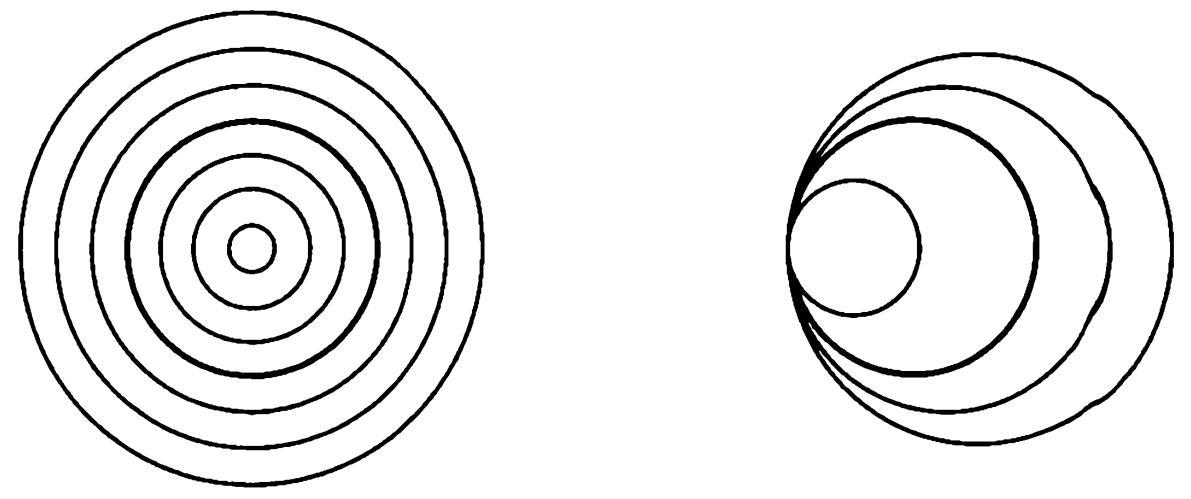
\includegraphics[width=1.0\textwidth]{images/11.1.jpg}
\end{center}
\hspace*{3em}

Figure 11.1
\end{example}

\begin{example} If \(\left( {{x}_{0},{y}_{0}}\right)\) and \(\left( {{x}_{1},{y}_{1}}\right)\) are two points of the plane \({\mathbb{R}}^{2}\) , define

\[
\left( {{x}_{0},{y}_{0}}\right)  \prec  \left( {{x}_{1},{y}_{1}}\right)
\]

If \({y}_{0} = {y}_{1}\) and \({x}_{0} < {x}_{1}\) This is a partial ordering of \({\mathbb{R}}^{2}\) under which two points are comparable only if they lie on the same horizontal line The maximal simply ordered sets are the horizontal lines in \({\mathbb{R}}^{2}\)
\end{example}

One can give an intuitive ``proof'' of the maximum principle that is rather appealing. It involves a step-by-step procedure, which one can describe in physical terms as follows. Suppose we take a box, and put into it some of the elements of \(A\) according to the following plan: First we pick an arbitrary element of \(A\) and put it in the box. Then we pick another element of \(A\) . If it is comparable with the element in the box, we put it in the box too; otherwise, we throw it away. At the general step, we will have a collection of elements in the box and a collection of elements that have been tossed away. Take one of the remaining elements of \(A\) If it is comparable with everything in the box, toss it in the box, too, otherwise, throw it away. Similarly continue. After you have checked all the elements of \(A\) , the elements you have in the box will be comparable with one another, and thus they will form a simply ordered set. Every element not in the box will be noncomparable with at least one element in the box, for that was why it was tossed away. Hence, the simply ordered set in the box is maximal, for no larger subset of \(A\) can satisfy the comparability condution

Now of course the weak point in the preceding ``proof'' comes when we said, ``After you have checked all the elements of \(A\) .'' How do you know you ever ``get through'' checking all the elements of \(A\) ? If \(A\) should happen to be countable, it is not hard to make this intuitive proof into a real proof. Let us take the countably infinite case; the finite case is even easier. Index the elements of \(A\) bijectively with the positive integers, so that \(A = \left\{  {{a}_{1},{a}_{2}\ldots }\right\}\) . This indexing gives a way of deciding what order to test the elements of \(A\) in, and how to know when one has tested them all.

Now we define a function \(h : {\mathbb{Z}}_{ + } \rightarrow  \{ 0,1\}\) , by letting it assign the value 0 to \(i\) if we ``put \({a}_{i}\) in the box,'' and the value 1 if we ``throw \({a}_{i}\) away.'' This means that \(h\left( 1\right)  = 0\) , and for \(i > 1\) , we have \(h\left( i\right)  = 0\) if and only if \({a}_{i}\) is comparable with every element of the set

\[
\left\{  {{a}_{j} \mid  j < i\text{ and }h\left( j\right)  = 0}\right\}  \text{ . }
\]

By the principle of recursive definition, this formula determines a unique function \(h.{\mathbb{Z}}_{ + } \rightarrow  \{ 0,1\}\) It is easy to check that the set of those \({a}_{j}\) for which \(h\left( j\right)  = 0\) is a maximal simply ordered subset of \(A\) .

If \(A\) is not countable, a variant of this procedure will work, if we allow ourselves to use the well-ordering theorem. Instead of indexing the elements of \(A\) with the set \({\mathbb{Z}}_{ + }\) , we index them (in a bijective fashion) with the elements of some well-ordered set \(J\) , so that \(A = \left\{  {{a}_{\alpha } \mid  \alpha  \in  J}\right\}\) . For this we need the well-ordering theorem, so that we know there is a bijection between \(A\) and some well-ordered set \(J\) . Then we can proceed as in the previous paragraph, letting \(\alpha\) replace \(i\) in the argument. Strictly speaking, you need to generalize the principle of recursive definition to well-ordered sets as well, but that is not particularly difficult. (See the Supplementary Exercises.)

Thus, the well-ordering theorem implies the maximum principle.

Although the maximum principle of Hausdorff was the first to be formulated and is probably the simplest to understand, there is another such principle that is nowadays the one most frequently quoted. It is popularly called ``\idx{Zorn's Lemma},'' although Ku-ratowski (1922) and Bochner (1922) preceded Zorn (1935) in enunciating and proving versions of it. For a history and discussion of the tangled history of these ideas, see \cite{Campbell1978} or \cite{Moore1982}. To state this principle, we need some terminology.

\begin{definition} Let \(A\) be a set and let \(\prec\) be a strict partial order on \(A\) . If \(B\) is a subset of \(A\) , an upper bound on \(B\) is an element \(c\) of \(A\) such that for every \(b\) in \(B\) , either \(b = c\) or \(b \prec  c\) . A \idx{maximal element} of \(A\) is an element \(m\) of \(A\) such that for no element \(a\) of \(A\) does the relation \(m \prec  a\) hold.
\end{definition}

Zorn's Lemma. Let \(A\) be a set that is strictly partially ordered. If every simply ordered subset of \(A\) has an upper bound in \(A\) , then \(A\) has a maximal element.

Zorn’s lemma is an easy consequence of the maximum principle: Given \(A\) , the maximum principle implies that \(A\) has a maximal simply ordered subset \(B\) . The hypothesis of Zorn’s lemma tells us that \(B\) has an upper bound \(c\) in \(A\) . The element \(c\) is then automatically a maximal element of \(A\) . For if \(c \prec  d\) for some element \(d\) of \(A\) , then the set \(B \cup  \{ d\}\) , which properly contains \(B\) , is simply ordered because \(b \prec  d\) for every \(b \in  B\) . This fact contradicts maximality of \(B\) .

It is also true that the maximum principle is an easy consequence of Zorn's lemma. See Exercises 5-7.

One final remark. We have defined what we mean by a strict partial order on a set, but we have not said what a partial order itself is. Let \(\prec\) be a strict partial order on a set \(A\) Suppose that we define \(a \preccurlyeq  b\) if either \(a \prec  b\) or \(a = b\) . Then the relation \(\preccurlyeq\) is called a partial order on \(A\) For example, the inclusion relation \(\subset\) on a collection of sets is a partial order, whereas proper inclusion is a strict partial order.

Many authors prefer to deal with partial orderings rather than strict partial orderings, the maximum principle and Zorn's lemma are often expressed in these terms. Which formulation is used is simply a matter of taste and convenience.

\section*{Exercises}

1. If \(a\) and \(b\) are real numbers, define \(a \prec  b\) if \(b - a\) is positive and rational. Show this is a strict partial order on \(\mathbb{R}\) . What are the maximal simply ordered subsets?

2. (a) Let \(\prec\) be a strict partial order on the set \(A\) . Define a relation on \(A\) by letting \(a \preccurlyeq  b\) if either \(a \prec  b\) or \(a = b\) . Show that this relation has the following properties, which are called the partial order axioms:

(i) \(a \preccurlyeq  a\) for all \(a \in  A\) .

(ii) \(a \preccurlyeq  b\) and \(b \preccurlyeq  a \Rightarrow  a = b\) .

(iii) \(a \preccurlyeq  b\) and \(b \preccurlyeq  c \Rightarrow  a \preccurlyeq  c\) .

(b) Let \(P\) be a relation on \(A\) that satisfies properties (i)-(iii). Define a relation \(S\) on \(A\) by letting \({aSb}\) if \({aPb}\) and \(a \neq  b\) . Show that \(S\) is a strict partial order on \(A\) .

3. Let \(A\) be a set with a strict partial order \(\prec\) ; let \(x \in  A\) . Suppose that we wish to find a maximal simply ordered subset \(B\) of \(A\) that contains \(x\) . One plausible way of attempting to define \(B\) is to let \(B\) equal the set of all those elements of \(A\) that are comparable with \(x\) ;

\[
B = \{ y \mid  y \in  A\text{ and either }x \prec  y\text{ or }y \prec  x\} .
\]

But this will not always work. In which of Examples 1 and 2 will this procedure succeed and in which will it not?

4. Given two points \(\left( {{x}_{0},{y}_{0}}\right)\) and \(\left( {{x}_{1},{y}_{1}}\right)\) of \({\mathbb{R}}^{2}\) , define

\[
\left( {{x}_{0},{y}_{0}}\right)  \prec  \left( {{x}_{1},{y}_{1}}\right)
\]

if \({x}_{0} < {x}_{1}\) and \({y}_{0} \leq  {y}_{1}\) . Show that the curves \(y = {x}^{3}\) and \(y = 2\) are maximal simply ordered subsets of \({\mathbb{R}}^{2}\) , and the curve \(y = {x}^{2}\) is not. Find all maximal simply ordered subsets.

5. Show that Zorn's lemma implies the following:

\begin{lemma}[Kuratowski] Let \(\mathcal{A}\) be a collection of sets. Suppose that for every subcollection \(\mathcal{B}\) of \(\mathcal{A}\) that is simply ordered by proper inclusion, the union of the elements of \(\mathcal{B}\) belongs to \(\mathcal{A}\) Then \(\mathcal{A}\) has an element that is properly contained in no other element of \(\mathcal{A}\) .
\end{lemma}

6. A collection \(\mathcal{A}\) of subsets of a set \(X\) is said to be of finite type provided that a subset \(B\) of \(X\) belongs to \(\mathcal{A}\) if and only if every finite subset of \(B\) belongs to \(\mathcal{A}\) . Show that the \idx{Kuratowski lemma} implies the following.

\begin{lemma}[Tukey, 1940] Let \(\mathcal{A}\) be a collection of sets. If \(\mathcal{A}\) is of finite type, then \(\mathcal{A}\) has an element that is properly contained in no other element of \(\mathcal{A}\) .
\end{lemma}

7. Show that the \idx{Tukey lemma} implies the \idx{Hausdorff maximum principle}. [Hint: If \(\prec\) is a strict partial order on \(A\) , let \(\mathcal{A}\) be the collection of all subsets of \(A\) that are simply ordered by \(\prec\) . Show that \(\mathcal{A}\) is of finite type.)

8. A typical use of Zorn's lemma in algebra is the proof that every vector space has a basis. Recall that if \(A\) is a subset of the vector space \(V\) , we say a vector belongs to the span of \(A\) if it equals a finite linear combination of elements of \(A\) . The set \(A\) is independent if the only finite linear combination of elements of \(A\) that equals the zero vector is the trivial one having all coefficients zero. If \(A\) is independent and if every vector in \(V\) belongs to the span of \(A\) , then \(A\) is a basis for \(V\) .

(a) If \(A\) is independent and \(v \in  V\) does not belong to the span of \(A\) , show \(A \cup  \{ v\}\) is independent.

(b) Show the collection of all independent sets in \(V\) has a maximal element.

(c) Show that \(V\) has a basis.

\section*{* Supplementary Exercises: Well-Ordering}

In the following exercises, we ask you to prove the equivalence of the choice axiom, the well-ordering theorem, and the maximum principle. We comment that of these exercises, only Exercise 7 uses the choice axiom.

1. Theorem (General principle of recursive definition). Let \(J\) be a well-ordered set; let \(C\) be a set. Let \(\mathcal{F}\) be the set of all functions mapping sections of \(J\) into \(C\) . Given a function \(\rho  : \mathcal{F} \rightarrow  C\) , there exists a unique function \(h : J \rightarrow  C\) such that \(h\left( \alpha \right)  = \rho \left( {h \mid  {S}_{\alpha }}\right)\) for each \(\alpha  \in  J\) .

[Hint: Follow the pattern outlined in Exercise 10 of \(§{10}\) .]

2. (a) Let \(J\) and \(E\) be well-ordered sets, let \(h : J \rightarrow  E\) . Show the following two statements are equivalent:

(i) \(h\) is order preserving and its image is \(E\) or a section of \(E\) .

(ii) \(h\left( \alpha \right)  =\) smallest \(\left\lbrack  {E - h\left( {S}_{\alpha }\right) }\right\rbrack\) for all \(\alpha\) .

[Hint: Show that each of these conditions implies that \(h\left( {S}_{\alpha }\right)\) is a section of \(E\) , conclude that it must be the section by \(h\left( \alpha \right)\) .]

(b) If \(E\) is a well-ordered set, show that no section of \(E\) has the order type of \(E\) , nor do two different sections of \(E\) have the same order type. [Hint: Given \(J\) , there is at most one order-preserving map of \(J\) into \(E\) whose image is \(E\) or a section of \(E\) .]

3. Let \(J\) and \(E\) be well-ordered sets; suppose there is an order-preserving map \(k : J \rightarrow  E\) . Using Exercises 1 and 2, show that \(J\) has the order type of \(E\) or a section of \(E\) . [Hint: Choose \({e}_{0} \in  E\) . Define \(h : J \rightarrow  E\) by the recursion formula

\[
h\left( \alpha \right)  = \text{ smallest }\left\lbrack  {E - h\left( {S}_{\alpha }\right) }\right\rbrack  \;\text{ if }\;h\left( {S}_{\alpha }\right)  \neq  E,
\]

and \(h\left( \alpha \right)  = {e}_{0}\) otherwise. Show that \(h\left( \alpha \right)  \leq  k\left( \alpha \right)\) for all \(\alpha\) ; conclude that \(\left. {h\left( {S}_{\alpha }\right)  \neq  E\text{ for all }\alpha .}\right\rbrack\)

4. Use Exercises 1-3 to prove the following

(a) If \(A\) and \(B\) are well-ordered sets, then exactly one of the following three conditions holds: \(A\) and \(B\) have the same order type, or \(A\) has the order type of a section of \(B\) , or \(B\) has the order type of a section of \(A\) . [Hint: Form a well-ordered set containing both \(A\) and \(B\) , as in Exercise 8 of \(§{10}\) ; then apply the preceding exercise.]

(b) Suppose that \(A\) and \(B\) are well-ordered sets that are uncountable, such that every section of \(A\) and of \(B\) is countable. Show \(A\) and \(B\) have the same order type.

5. Let \(X\) be a set; let \(\mathcal{A}\) be the collection of all pairs \(\left( {A, < }\right)\) , where \(A\) is a subset of \(X\) and \(<\) is a well-ordering of \(A\) . Define

\[
\left( {A, < }\right)  \prec  \left( {{A}^{\prime },{ < }^{\prime }}\right)
\]

if \(\left( {A, < }\right)\) equals a section of \(\left( {{A}^{\prime },{ < }^{\prime }}\right)\) .

(a) Show that \(\prec\) is a strict partial order on \(\mathcal{A}\) .

(b) Let \(\mathcal{B}\) be a subcollection of \(\mathcal{A}\) that is simply ordered by \(\prec\) . Define \({B}^{\prime }\) to be the union of the sets \(B\) , for all \(\left( {B, < }\right)  \in  \mathcal{B}\) ; and define \({ < }^{\prime }\) to be the union of the relations \(<\) , for all \(\left( {B, < }\right)  \in  \mathcal{B}\) . Show that \(\left( {{B}^{\prime },{ < }^{\prime }}\right)\) is a well-ordered set.

6. Use Exercises 1 and 5 to prove the following:

\begin{theorem} The maximum principle is equivalent to the well-ordering theorem.
\end{theorem}

7. Use Exercises 1-5 to prove the following.

\begin{theorem} The choice axiom is equivalent to the well-ordering theorem.
\end{theorem}
\begin{proof} Let \(X\) be a set, let \(c\) be a fixed choice function for the nonempty subsets of \(X\) . If \(T\) is a subset of \(X\) and \(<\) is a relation on \(T\) , we say that \(\left( {T, < }\right)\) is a tower in \(X\) if \(<\) is a well-ordering of \(T\) and if for each \(x \in  T\) ,

\[
x = c\left( {X - {S}_{x}\left( T\right) }\right) ,
\]

where \({S}_{x}\left( T\right)\) is the section of \(T\) by \(x\) .

(a) Let \(\left( {{T}_{1},{ < }_{1}}\right)\) and \(\left( {{T}_{2},{ < }_{2}}\right)\) be two towers in \(X\) . Show that either these two ordered sets are the same, or one equals a section of the other. [Hint: Switching indices if necessary, we can assume that \(h : {T}_{1} \rightarrow  {T}_{2}\) is order preserving and \(h\left( {T}_{1}\right)\) equals either \({T}_{2}\) or a section of \({T}_{2}\) . Use Exercise 2 to show that \(h\left( x\right)  = x\) for all \(x\) .]

(b) If \(\left( {T, < }\right)\) is a tower in \(X\) and \(T \neq  X\) , show there is a tower in \(X\) of which \(\left( {T, < }\right)\) is a section.

(c) Let \(\left\{  {\left( {{T}_{k},{ < }_{k}}\right)  \mid  k \in  K}\right\}\) be the collection of all towers in \(X\) . Let

\[
T = \mathop{\bigcup }\limits_{{k \in  K}}{T}_{k}\;\text{ and }\; <  = \mathop{\bigcup }\limits_{{k \in  K}}\left( { < }_{k}\right) .
\]

Show that \(\left( {T, < }\right)\) is a tower in \(X\) . Conclude that \(T = X\) .

8. Using Exercises 1-4, construct an uncountable well-ordered set, as follows. Let \(A\) be the collection of all pairs \(\left( {A, < }\right)\) , where \(A\) is a subset of \({\mathbb{Z}}_{ + }\) and \(<\) is a well-ordering of \(A\) . (We allow \(A\) to be empty.) Define \(\left( {A, < }\right)  \sim  \left( {{A}^{\prime },{ < }^{\prime }}\right)\) if \(\left( {A, < }\right)\) and \(\left( {{A}^{\prime },{ < }^{\prime }}\right)\) have the same order type. It is trivial to show this is an equivalence relation. Let \(\left\lbrack  \left( {A, < }\right) \right\rbrack\) denote the equivalence class of \(\left( {A, < }\right)\) ; let \(E\) denote the collection of these equivalence classes. Define

\[
\left\lbrack  \left( {A, < }\right) \right\rbrack \ll  \left\lbrack  \left( {{A}^{\prime },{ < }^{\prime }}\right) \right\rbrack
\]

if \(\left( {A, < }\right)\) has the order type of a section of \(\left( {{A}^{\prime },{ < }^{\prime }}\right)\) .

(a) Show that the relation \(\ll\) is well defined and is a simple order on \(E\) . Note that the equivalence class \(\left\lbrack  \left( {\varnothing ,\varnothing }\right) \right\rbrack\) is the smallest element of \(E\) .

(b) Show that if \(\alpha  = \left\lbrack  \left( {A, < }\right) \right\rbrack\) is an element of \(E\) , then \(\left( {A, < }\right)\) has the same order type as the section \({S}_{\alpha }\left( E\right)\) of \(E\) by \(\alpha\) . [Hint: Define a map \(f : A \rightarrow  E\) by setting \(f\left( x\right)  = \left\lbrack  \left( {{S}_{x}\left( A\right) \text{ , restriction of } < }\right) \right\rbrack\) for each \(x \in  A\) .]

(c) Conclude that \(E\) is well-ordered by \(\ll\) .

(d) Show that \(E\) is uncountable. [Hint: If \(h : E \rightarrow  {\mathbb{Z}}_{ + }\) is a bijection, then \(h\) gives rise to a well-ordering of \({\mathbb{Z}}_{ + }\) .]
\end{proof}

This same argument, with \({\mathbb{Z}}_{ + }\) replaced by an arbitrary well-ordered set \(X\) , proves (without use of the choice axiom) the existence of a well-ordered set \(E\) whose cardinality is greater than that of \(X\) .

This exercise shows that one can construct an uncountable well-ordered set, and hence the minimal uncountable well-ordered set, by an explicit construction that does not use the choice axiom. However, this result is less interesting than it might appear. The crucial property of \({S}_{\Omega }\) , the one we use repeatedly, is the fact that every countable subset of \({S}_{\Omega }\) has an upper bound in \({S}_{\Omega }\) . That fact depends, in turn, on the fact that a countable union of countable sets is countable. And the proof of that result (if you examine it carefully) involves an infinite number of arbitrary choices-that is, it depends on the choice axiom.

Said differently, without the choice axiom we may be able to construct the minimal uncountable well-ordered set, but we can't use it for anything!
\chapter[\index{topological space@Topological space}\index{topological space@Topological space}Topological Spaces \index{Quotient topology!and continuous functions}\index{Quotient topology!and continuous functions}and Continuous Functions]{Topological Spaces \\and Continuous Functions}
\vspace{6.5cm}

The concept of topological \index{First-countable space (see First-countability)} space grew out of the study of the real line and euclidean space and the study of \index{continuous function} on these spaces. In this chapter, we define what a \index{Topological space}\index{Topological space}topological space is, and we study a number of ways of constructing a \index{topology} on a set so as to make it into a topological space. We also consider some of the elementary concepts associ\index{Continuity: of algebraic operations in \(\mathbb{R}\)!at a point}\index{Continuity: of algebraic operations in \(\mathbb{R}\)!at a point}ated with topological spaces. Open and \index{closed set}, \index{limit point}, \index{Quotient topology!and continuous functions}\index{Quotient topology!and continuous functions}\index{Sequences!and closure}and cont\index{Closure!in a cartesian product}inuous functions are introduced as natural \index{Cartesian product: countably infinite!general}\index{Cartesian product: countably infinite!general}\index{Cartesian product: countably infinite!general}\index{Cartesian product: countably infinite!general}generalizations of the corresponding ideas for the real line and euclidean space.

\section*{§ 12 Topological Spaces}

The definition of a topological space that is now \index{Standard topology: on} standard was a long time in being formulated. Various mathematicians-Fréchet, Hausdorff, and others-proposed different definitions over a period of years during the first decades of the twentieth century, but it took quite a while before mathematicians settled on the one that seemed most suitable. They wanted, of course, a definition that was as broad as possible, so that it would include as special cases all the various examples that were useful in mathematics-euclidean space, \index{infinite series} infinite-dimensional euclidean space, and function spaces among them-but they also wanted the definition to be narrow enough that the standard theorems about these familiar spaces would hold for topological spaces in general. This is always the problem when one is trying to formulate a new mathematical concept, to decide how general its definition should be. The definition finally settled on may seem a bit abstract, but as you work through the various ways of constructing topological spaces, you will get a better feeling for what the concept means.

\begin{definition}
	A \index{Topology}\index{Topology}\index{topology@Topology}\index{topology@Topology}topology on a set \(X\) is a collection \(\mathcal{T}\) of subsets of \(X\) having the following properties:

(1) \(\varnothing\) and \(X\) are in \(\mathcal{T}\) .

(2) The union of the elements of any subcollection of \(\mathcal{T}\) is in \(\mathcal{T}\) .

(3) The intersection of the elements of any finite subcollection of \(\mathcal{T}\) is in \(\mathcal{T}\) .

A set \(X\) for which a topology \(\mathcal{T}\) has been specified is called a topological space.

Properly speaking, a topological space is an \index{Ray in ordered set} ordered pair(X, T)consisting \index{Interior point: of an arc!of a set}\index{Interior point: of an arc!of a set}\index{Interior point: of an arc!of a set}\index{Interior point: of an arc!of a set}of a set \(X\) and a topology \(\mathcal{T}\) on \(X\) , but we often omit specific mention of \(\mathcal{T}\) if no confusion will anse.
\end{definition}


If \(X\) is a topological space with topology \(\mathcal{T}\) , we say that a subset \(U\) of \(X\) is an \index{open set} of \(X\) if \(U\) belongs to the collection \(\mathcal{T}\) . Using this terminology, one can say that a topological space is a set \(X\) together with a collection of subsets of \(X\) , called \index{Open set}\index{Open set}\index{open set@Open set}\index{open set@Open set}open sets, such that \(\varnothing\) and \(X\) are both open, and such that arbitrary unions and finite intersections of open sets are open.

\begin{centeredblock}
\begin{example}
	Let \(X\) be a three-element set, \(X = \{ a,b,c\}\) There are many possible topologies on \(X\) , some of which are indicated schematically in Figure 12.1. The diagram in the upper right-hand corner indicates the topology in which the open sets are \(X,\varnothing\) , \(\{ a,b\} ,\{ b\}\) , and \(\{ b,c\}\) The topology in the upper left-hand corner contains only \(X\) and \(\varnothing\) , while the topology in the lower right-hand corner contains every subset \index{Comparability: of cardinalities!of topologies}\index{Comparability: of cardinalities!of topologies}of \(X\) . You can get other topologies on \(X\) by permuting \(a,b\) , and \(c\)

\begin{center}
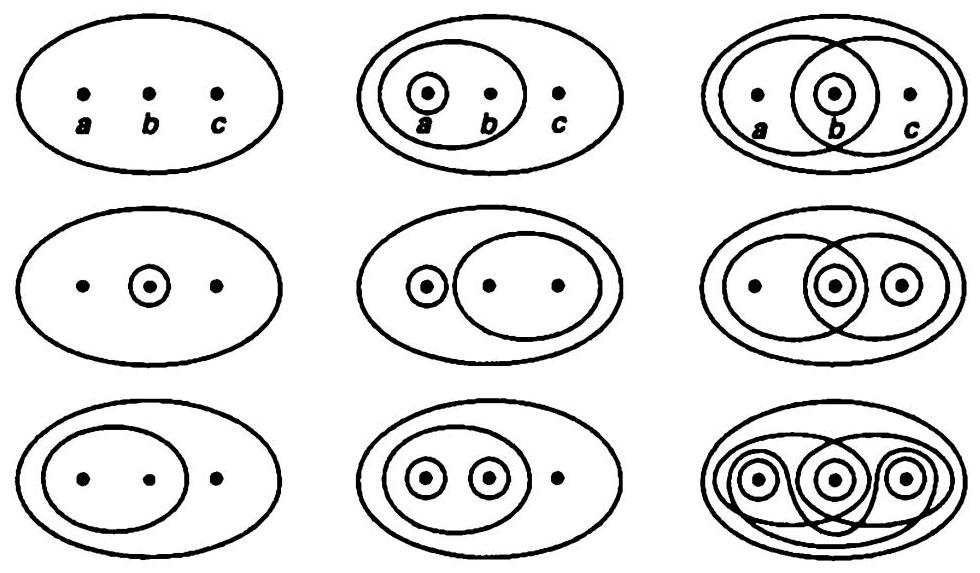
\includegraphics[width=0.9\textwidth]{images/12.1.jpg}
\end{center}
\hspace*{3em}

Figure 12.1
\end{example}
\end{centeredblock}

From this example, you can see that even a three-element set has many different topologies. But not every collection of subsets of \(X\) is a topology on \(X\) Neither of the collections inducated in Figure 122 is a topology, for instance.

\begin{center}
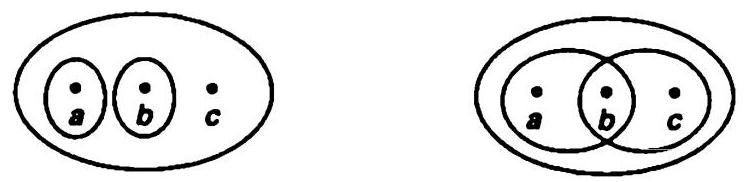
\includegraphics[width=0.6\textwidth]{images/12.2.jpg}
\end{center}
\hspace*{3em}

Figure 12.2

\begin{centeredblock}
\begin{example}
	If \(X\) is any set, the collection of all subsets of \(X\) is a topology on \(X\) , it is called the \index{discrete topology} The collection consisting of \(X\) and \(\varnothing\) only is also a topology on \(X\) ; we shall call it the \index{indiscrete topology}, or the \index{trivial topology}
\end{example}
\end{centeredblock}

\begin{centeredblock}
\begin{example}
	Let \(X\) be a set, let \({\mathcal{T}}_{f}\) be the collection of all subsets \(U\) of \(X\) such that \(X - U\) either is finite or is all of \(X\) Then \({\mathcal{T}}_{f}\) is a topology on \(X\) , called the \index{finite complement topology}. Both \(X\) and \(\varnothing\) are in \({\mathcal{T}}_{f}\) , since \(X - X\) is finite and \(X - \varnothing\) is all of \(X\) If \(\{  {U}_{\alpha }\}\) is an indexed family of nonempty elements of \({\mathcal{T}}_{f}\) , to show that \(\bigcup {U}_{\alpha }\) is in \({\mathcal{T}}_{f}\) , we compute

\[
X - \bigcup {U}_{\alpha } = \bigcap ( {X - {U}_{\alpha }})
\]

The latter set is finite because each set \(X - {U}_{\alpha }\) is finite If \({U}_{1},\;,{U}_{n}\) are nonempty elements of \({\mathcal{T}}_{f}\) , to show that \(\bigcap {U}_{t}\) is in \({\mathcal{T}}_{f}\) , we compute

\[
X - \mathop{\bigcap }\limits_{{i = 1}}^{n}{U}_{i} = \mathop{\bigcup }\limits_{{i = 1}}^{n}( {X - {U}_{i}})
\]

The latter set is a finite union of finite sets and, therefore, finite
\end{example}
\end{centeredblock}

\begin{centeredblock}
\begin{example}
	Let \(X\) be a set, let \({\mathcal{T}}_{c}\) be the collection of all subsets \(U\) of \(X\) such that \(X - U\) either is \index{Countable basis at a point} countable or is all of \(X\) . Then \({\mathcal{T}}_{c}\) is a topology on \(X\) , as you can check
\end{example}
\end{centeredblock}

\begin{definition}
	Suppose that \(\mathcal{T}\) and \({\mathcal{T}}^{\prime }\) are two topologies on a given set \(X\) . If \({\mathcal{T}}^{\prime } \supset  \mathcal{T}\) , we say that \({\mathcal{T}}^{\prime }\) is \index{Finer topology} finer than \(\mathcal{T}\) ; if \({\mathcal{T}}^{\prime }\) properly contains \(\mathcal{T}\) , we say that \({\mathcal{T}}^{\prime }\) is \index{Strictly coarser topology} strictly finer than \(\mathcal{T}\) . We also say that \(\mathcal{T}\) is \index{Coarser topology} coarser than \({\mathcal{T}}^{\prime }\) , or strictly coarser, in these two respective situations. We say \(\mathcal{T}\) is comparable with \({\mathcal{T}}^{\prime }\) if either \({\mathcal{T}}^{\prime } \supset  \mathcal{T}\) or \(\mathcal{T} \supset  {\mathcal{T}}^{\prime }\) .
\end{definition}


This terminology is suggested by thinking of a topological space as being something like a truckload full \index{Closure!of a union}\index{Closure!of a union}of gravel--the pebbles and all unions of collections of pebbles being the open sets. If now we smash the pebbles into \index{Smaller topology} \index{smaller topology@Smaller topology}\index{smaller topology@Smaller topology}smaller ones, the collection of open sets has been enlarged, and the topology, like the gravel, is said to have been made finer by the operation.

Two topologies on \(X\) need not be comparable, of course. In Figure 121 preceding, the topology in the upper right-hand corner is strictly finer than each of the three topologies in the first column and strictly coarser than each of the other topologies in the third column. But it is not comparable with any of the topologies in the second column.

Other terminology is sometimes used for this concept. If \({\mathcal{T}}^{\prime } \supset  \mathcal{T}\) , some mathematicians would say that \({\mathcal{T}}^{\prime }\) is \index{Larger topology} larger than \(\mathcal{T}\) , and \(\mathcal{T}\) is smaller than \({\mathcal{T}}^{\prime }\) . This is certainly acceptable terminology, if not as vivid as the words ``\index{finer topology@Finer topology}finer'' and ``\index{coarser topology@Coarser topology}\index{coarser topology@Coarser topology}coarser.''

Many mathematicians use the words ``\index{Weaker topology} \index{weaker topology@Weaker topology}\index{weaker topology@Weaker topology}weaker'' and ``\index{Stronger topology} stronger'' in this context. Unfortunately, some of them (particularly analysts) are apt to say that \({\mathcal{T}}^{\prime }\) is stronger than \(\mathcal{T}\) if \({\mathcal{T}}^{\prime } \supset  \mathcal{T}\) , while others (particularly topologists) are apt to say that \({\mathcal{T}}^{\prime }\) is weaker than \(\mathcal{T}\) in the same situation! If you run across the terms ``strong topology'' or ``weak topology'' in some book, you will have to decide from the context which inclusion is meant. We shall not use these terms in this book.

\section*{§ 13 Basis for a Topology}

For each of the examples in the preceding section, we were able to specify the topology by describing the entire collection \(\mathcal{T}\) of open sets. Usually this is too difficult. In most cases, one specifies instead a smaller collection of subsets of \(X\) and defines the topology in terms of that.

\begin{definition}
	If \(X\) is a set, a \index{Box topology!basis for}\index{Box topology!basis for}\index{Box topology!basis for}\index{Box topology!basis for}basis for a topology on \(X\) is a collection \(\mathcal{B}\) of subsets of \(X\) (called basis elements) such that

(1) For each \(x \in  X\) , there is at least one basis element \(B\) containing \(x\) .

(2) If \(x\) belongs to the intersection of two basis elements \({B}_{1}\) and \({B}_{2}\) , then there is a basis element \({B}_{3}\) containing \(x\) such that \({B}_{3} \subset  {B}_{1} \cap  {B}_{2}\) .

If \(\mathcal{B}\) satisfies these two conditions, then we define the topology \(\mathcal{T}\) generated by \(\mathcal{B}\) as follows: \(A\) subset \(U\) of \(X\) is said to be open in \(X\) (that is, to be an element of \(\mathcal{T}\) ) if for each \(x \in  U\) , there is a basis element \(B \in  \mathcal{B}\) such that \(x \in  B\) and \(B \subset  U\) . Note that each basis element is itself an element of \(\mathcal{T}\) .
\end{definition}

We will check shortly that the collection \(\mathcal{T}\) is indeed a topology on \(X\) . But first let us consider some examples.


\begin{centeredblock}
\begin{example}
	Let \(\mathcal{B}\) be the collection of all circular regions (interiors of circles) in the plane. Then \(\mathcal{B}\) satisfies both conditions for a basis The second condition is illustrated in Figure 13 1. In the topology generated by \(\mathcal{B}\) , a subset \(U\) of the plane is open if every \(x\) in \(U\) lies in some circular region contained in \(U\)

\begin{center}
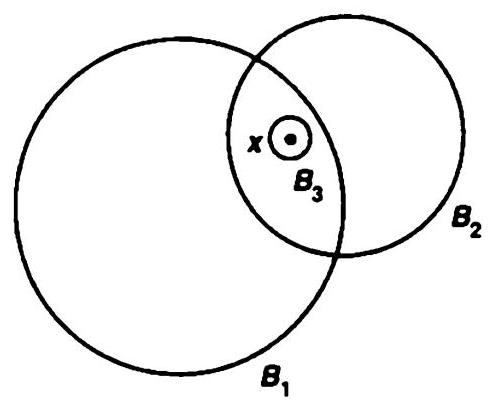
\includegraphics[width=0.4\textwidth]{images/13.1.jpg}
\end{center}
\hspace*{3em}

Figure 13.1

\begin{center}
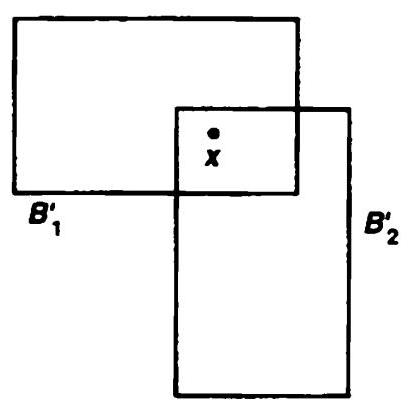
\includegraphics[width=0.3\textwidth]{images/13.2.jpg}
\end{center}
\hspace*{3em}

Figure 13.2
\end{example}
\end{centeredblock}

\begin{centeredblock}
\begin{example}
	Let \({\mathcal{B}}^{\prime }\) be the collection of all rectangular regions (interiors of rectangles) in the plane, where the rectangles have sides parallel to the \index{Coordinate: of J-tuple} coordinate axes Then \({\mathcal{B}}^{\prime }\) satisfies both conditions for a basis. The second condition is illustrated in Figure 132; in thus case, the condition is tri\index{Closure!via basis elements}\index{Closure!via basis elements}vial, because the intersection of any two basis elements is itself a basis element (or empty) As we shall see later, the basis \({\mathcal{B}}^{\prime }\) generates the same topology on the plane as the basis \(\mathcal{B}\) given in the preceding example
\end{example}
\end{centeredblock}

\begin{centeredblock}
\begin{example}
	If \(X\) is any set, the collection \index{Continuity: of algebraic operations in \(\mathbb{R}\)!of metric}of all one-point subsets of \(X\) is a basis \index{Metric!for discrete topology}\index{Metric!for discrete topology}for the \index{Discrete topology}\index{Discrete topology}\index{discrete topology@Discrete topology}\index{discrete topology@Discrete topology}discrete topology on \(X\)
\end{example}
\end{centeredblock}

Let us check now that the collection \(\mathcal{T}\) generated by the basis \(\mathcal{B}\) is, in fact, a topology on \(X\) . If \(U\) is the empty set, it satisfies the defining condition of openness vacuously. Likewise, \(X\) is in \(\mathcal{T}\) , since for each \(x \in  X\) there is some basis element \(B\) containing \(x\) and contained in \(X\) Now let us take an indexed family \({\{  {U}_{\alpha }\}  }_{\alpha  \in  J}\) , of elements of \(\mathcal{T}\) and show that

\[
U = \mathop{\bigcup }\limits_{{\alpha  \in  J}}{U}_{\alpha }
\]

belongs to \(\mathcal{T}\) . Given \(x \in  U\) , there is an index \(\alpha\) such that \(x \in  {U}_{\alpha }\) . Since \({U}_{\alpha }\) is open, there is a basis element \(B\) such that \(x \in  B \subset  {U}_{\alpha }\) . Then \(x \in  B\) and \(B \subset  U\) , so that \(U\) is open, by definition.

Now let us take two elements \({U}_{1}\) and \({U}_{2}\) of \(\mathcal{T}\) and show that \({U}_{1} \cap  {U}_{2}\) belongs to \(\mathcal{T}\) . Given \(x \in  {U}_{1} \cap  {U}_{2}\) , choose a basis element \({B}_{1}\) containing \(x\) such that \({B}_{1} \subset  {U}_{1}\) ; choose also a basis element \({B}_{2}\) containing \(x\) such that \({B}_{2} \subset  {U}_{2}\) . The second condition for a basis enables us to choose a basis element \({B}_{3}\) containing \(x\) such that \({B}_{3} \subset  {B}_{1} \cap  {B}_{2}\) . See Figure 13.3. Then \(x \in  {B}_{3}\) and \({B}_{3} \subset  {U}_{1} \cap  {U}_{2}\) , so \({U}_{1} \cap  {U}_{2}\) belongs to \(\mathcal{T}\) , by definition.

\begin{center}
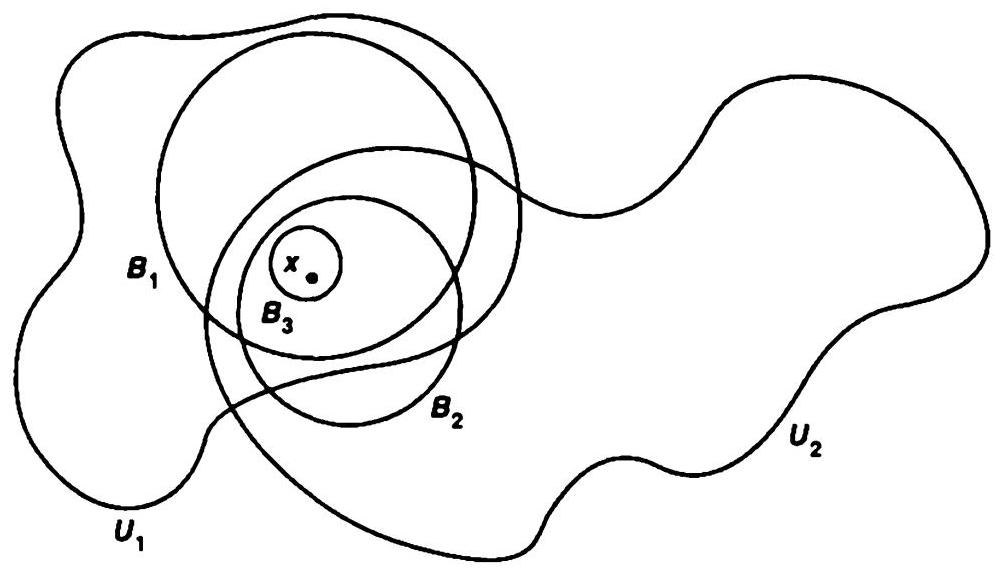
\includegraphics[width=0.9\textwidth]{images/13.3.jpg}
\end{center}
\hspace*{3em} 

Figure 13.3

Finally, we show by induction that any finite intersection \({U}_{1} \cap  \cdots  \cap  {U}_{n}\) of elements of \(\mathcal{T}\) is in \(\mathcal{T}\) . This fact is trivial for \(n = 1\) ; we suppose it true for \(n - 1\) and prove it for \(n\) . Now

\[
( {{U}_{1} \cap   \cdot   \cap  {U}_{n}})  = ( {{U}_{1} \cap  \cdots  \cap  {U}_{n - 1}})  \cap  {U}_{n}
\]

By hypothesis, \({U}_{1} \cap   \cdot   \cdot   \cap  {U}_{n - 1}\) belongs to \(\mathcal{T}\) ; by the result just proved, the intersection of \({U}_{1} \cap  \cdots  \cap  {U}_{n - 1}\) and \({U}_{n}\) also belongs to \(\mathcal{T}\)

Thus we have checked that collection of open sets \index{Topology!generated by a basis}\index{Topology!generated by a basis}\index{Topology!generated by a basis}\index{Topology!generated by a basis}generated by a basis \(\mathcal{B}\) is, in fact, a topology.

Another way of describing the topology generated by a basis is given in the following lemma.

\begin{lemma}
	Let \(X\) be a set; let \(\mathcal{B}\) be a basis for a topology \(\mathcal{T}\) on \(X\) . Then \(\mathcal{T}\) equals the collection of all unions of elements of \(\mathcal{B}\) .
\end{lemma}

\begin{proof}
Given a collection of elements of \(\mathcal{B}\) , they are also elements of \(\mathcal{T}\) . Because \(\mathcal{T}\) is a topology, their union is in \(\mathcal{T}\) . Conversely, given \(U \in  \mathcal{T}\) , choose for each \(x \in  U\) an element \({B}_{x}\) of \(\mathcal{B}\) such that \(x \in  {B}_{x} \subset  U\) . Then \(U = \mathop{\bigcup }\limits_{{x \in  U}}{B}_{x}\) , so \(U\) equals a union of elements of \(\mathcal{B}\) .

This lemma states that every open set \(U\) in \(X\) can be expressed as a union of basis elements. This expression for \(U\) is not, however, unique. Thus the use of the term ``basis'' in topology differs drastically from its use in linear algebra, where the equation expressing a given vector as a linear combination of basis vectors is unique.

We have described in two different ways how to go from a basis to the topology it generates. Sometimes we need to go in the reverse direction, from a topology to a basis generating it. Here is one way of obtaining a basis for a given topology; we shall use it frequently.
\end{proof}

\begin{lemma}
	Let \(X\) be a topological space. Suppose that \(\mathcal{C}\) is a collection of open sets of \(X\) such that for each open set \(U\) of \(X\) and each \(x\) in \(U\) , there is an element \(C\) of \(\mathcal{C}\) such that \(x \in  C \subset  U\) . Then \(\mathcal{C}\) is a basis for the topology of \(X\) .
\end{lemma}

\begin{proof}
We must show that \(\mathcal{C}\) is a basis. The first condition for a basis is easy: Given \(x \in  X\) , since \(X\) is itself an open set, there is by hypothesis an element \(C\) of \(\mathcal{C}\) such that \(x \in  C \subset  X\) . To check the second condition, let \(x\) belong to \({C}_{1} \cap  {C}_{2}\) , where \({C}_{1}\) and \({C}_{2}\) are elements of \(\mathcal{C}\) . Since \({C}_{1}\) and \({C}_{2}\) are open, so is \({C}_{1} \cap  {C}_{2}\) . Therefore, there exists by hypothesis an element \({C}_{3}\) in \(\mathcal{C}\) such that \(x \in  {C}_{3} \subset  {C}_{1} \cap  {C}_{2}\) .

Let \(\mathcal{T}\) be the collection of open sets of \(X\) ; we must show that the topology \({\mathcal{T}}^{\prime }\) generated by \(\mathcal{C}\) equals the topology \(\mathcal{T}\) . First, note that if \(U\) belongs to \(\mathcal{T}\) and if \(x \in  U\) , then there is by hypothesis an element \(C\) of \(\mathcal{C}\) such that \(x \in  C \subset  U\) . It follows that \(U\) belongs to the topology \({\mathcal{T}}^{\prime }\) , by definition. Conversely, if \(W\) belongs to the topology \({\mathcal{T}}^{\prime }\) , then \(W\) equals a union of elements of \(\mathcal{C}\) , by the preceding lemma. Since each element of \(\mathcal{C}\) belongs to \(\mathcal{T}\) and \(\mathcal{T}\) is a topology, \(W\) also belongs to \(\mathcal{T}\) .

When topologies are given by bases, it is useful to have a criterion in terms of the bases for determining whether one topology is finer than another. One such criterion is the following.
\end{proof}

\begin{lemma}
	Let \(\mathcal{B}\) and \({\mathcal{B}}^{\prime }\) be bases for the topologies \(\mathcal{T}\) and \({\mathcal{T}}^{\prime }\) , respectively, on \(X\) . Then the following are equivalent:

(1) \({\mathcal{T}}^{\prime }\) is finer than \(\mathcal{T}\) .

(2) For each \(x \in  X\) and each basis element \(B \in  \mathcal{B}\) containing \(x\) , there is a basis element \({B}^{\prime } \in  {\mathcal{B}}^{\prime }\) such that \(x \in  {B}^{\prime } \subset  B\) .
\end{lemma}

\begin{proof}
(2) \(\Rightarrow\) (1). Given an element \(U\) of \(\mathcal{T}\) , we wish to show that \(U \in  {\mathcal{T}}^{\prime }\) . Let \(x \in  U\) . Since \(\mathcal{B}\) generates \(\mathcal{T}\) , there is an element \(B \in  \mathcal{B}\) such that \(x \in  B \subset  U\) . Condition (2) tells us there exists an element \({B}^{\prime } \in  {\mathcal{B}}^{\prime }\) such that \(x \in  {B}^{\prime } \subset  B\) . Then \(x \in  {B}^{\prime } \subset  U\) , so \(U \in  {\mathcal{T}}^{\prime }\) , by definition.

(1) \(\Rightarrow\) (2). We are given \(x \in  X\) and \(B \in  \mathcal{B}\) , with \(x \in  B\) . Now \(B\) belongs to \(\mathcal{T}\) by definition and \(\mathcal{T} \subset  {\mathcal{T}}^{\prime }\) by condition (1); therefore, \(B \in  {\mathcal{T}}^{\prime }\) Since \({\mathcal{T}}^{\prime }\) is generated by \({\mathcal{B}}^{\prime }\) , there is an element \({B}^{\prime } \in  {\mathcal{B}}^{\prime }\) such that \(x \in  {B}^{\prime } \subset  B\) .

Some students find this condition hard to remember. ``Which way does the inclusion go?'' they ask. It may be easier to remember if you recall the analogy between a topological space and a truckload full of gravel. Think of the pebbles as the basis elements of the topology; after the pebbles are smashed to dust, the dust particles are the basis elements of the new topology. The new topology is finer than the old one, and each dust particle was contained inside a pebble, as the criterion states.
\end{proof}

\begin{centeredblock}
\begin{example}
	One can now see that the collection \(\mathcal{B}\) of all circular regions in the plane generates the same topology as the collection \({\mathcal{B}}^{\prime }\) of all rectangular regions, Figure 134 illustrates the pro\\index{Subspace topology!in metric space}index{First-countability!of metric space}\index{First-countability!of metric space}of We shall treat this example more \\index{Convergent sequence!in Hausdorff space}index{Hausdorff condition!for metric space}\index{Hausdorff condition!for metric space}formally when we study \\\index{Closure!in a subspace}index{Subspace topology!in metric space}index{\index{metric space@Metric space}metric space}

\begin{center}
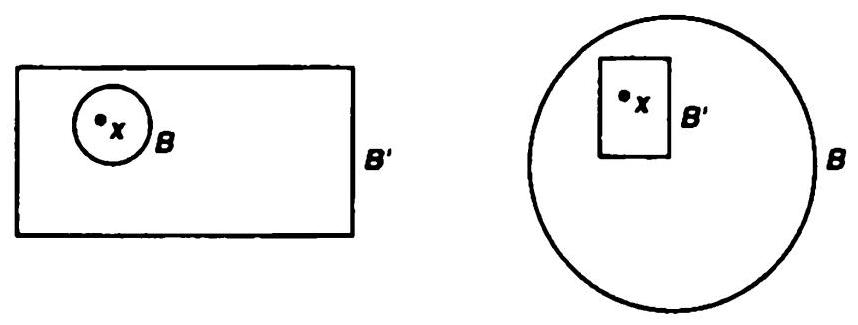
\includegraphics[width=0.7\textwidth]{images/13.4.jpg}
\end{center}
\hspace*{3em}

Figure 13.4
\end{example}
\end{centeredblock}

We now define three topologies on the real line \(\mathbb{R}\) , all of which are of interest.

\begin{definition}
	If \(\mathcal{B}\) is the collection of all open intervals in the real line,

\[
( {a,b})  = \{ x \mid  a < x < b\} ,
\]

the topology generated by \(\mathcal{B}\) is called the \index{\(\mathbb{R}\) (reals)!standard topology}\index{\(\mathbb{R}\) (reals)!standard topology}\index{\(\mathbb{R}\) (reals)!standard topology}\index{\(\mathbb{R}\) (reals)!standard topology}standard topology on the real line. Whenever we consider \(\mathbb{R}\) , we shall suppose it is given this topology unless we specifically state otherwise.
\end{definition}


If \({\mathcal{B}}^{\prime }\) is the collection of all \index{half-open interval} of the form

\[
\lbrack a,b) = \{ x \mid  a \leq  x < b\} ,
\]

where \(a < b\) , the topology generated by \({\mathcal{B}}^{\prime }\) is called the lower limit topology on \(\mathbb{R}\) . When \(\mathbb{R}\) is given the lower limit topology, we denote it by \(\index{R@\({\mathbb{R}}_{\ell }\)} \index{R@${\mathbb{R}}_{\ell }$}{\mathbb{R}}_{\ell }\) . Finally let \(K\) denote the set of all numbers of the form \(1/n\) , for \(n \in  {\mathbb{Z}}_{ + }\) , and let \({\mathcal{B}}^{\prime \prime }\) be the collection of all open intervals(a, b), along with all sets of the form \(( {a,b})  - K\) . The topology generated by \({\mathcal{B}}^{\prime \prime }\) will be called the \(K\) -topology on \(\mathbb{R}\) . When \(\mathbb{R}\) is given this topology, we denote it by \(\index{R@\({\mathbb{R}}_{K}\)} \index{R@${\mathbb{R}}_{K}$}{\mathbb{R}}_{K}\) .

It is easy to see that all three of these collections are bases; in each case, the intersection of two basis elements is either another basis element or is empty. The relation between these topologies is the following

\begin{lemma}
	The topologies of \({\mathbb{R}}_{\ell }\) and \({\mathbb{R}}_{K}\) are strictly finer than the standard topology on \(\mathbb{R}\) , but are not comparable with one another.
\end{lemma}

Proof Let \(\mathcal{T},{\mathcal{T}}^{\prime }\) , and \({\mathcal{T}}^{\prime \prime }\) be the topologies of \(\mathbb{R},{\mathbb{R}}_{\ell }\) , and \({\mathbb{R}}_{K}\) , respectively. Given a basis element(a, b)for \(\mathcal{T}\) and a point \(x\) of(a, b), the basis element \(\lbrack x,b)\) for \({\mathcal{T}}^{\prime }\) contains \(x\) and lies in(a, b). On the other hand, given the basis element \(\lbrack x,d)\) for \({\mathcal{T}}^{\prime }\) , there is no open interval(a, b)that contains \(x\) and lies in \(\lbrack x,d)\) . Thus \({\mathcal{T}}^{\prime }\) is strictly finer than \(\mathcal{T}\)

A similar argument applies to \({\mathbb{R}}_{K}\) . Given a basis element(a, b)for \(\mathcal{T}\) and a point \(x\) of(a, b), this same interval is a basis element for \({\mathcal{T}}^{\prime \prime }\) that contains \(x\) . On the other hand, given the basis element \(B = ( {-1,1})  - K\) for \({\mathcal{T}}^{\prime \prime }\) and the point0of \(B\) , there is no open interval that contains 0 and lies in \(B\) .

We leave it to you to show that the topologies of \({\mathbb{R}}_{\ell }\) and \({\mathbb{R}}_{K}\) are not comparable.

A question may occur to you at this point. Since the topology generated by a basis \(\mathcal{B}\) may be described as the collection of arbitrary unions of elements of \(\mathcal{B}\) , what happens if you start with a given collection of sets and take finite intersections of them as well as arbitrary unions? This question leads to the notion of a \index{subbasis} for a topology

\begin{definition}
	A \index{Order topology!subbasis}subbasis \(S\) for a topology on \(X\) is a collection of subsets of \(X\) whose union equals \(X\) . The topology generated by the subbasis \(S\) is defined to be the collection \(\mathcal{T}\) of all unions of finite intersections of elements of \(\mathcal{S}\) .
\end{definition}


We must of course check that \(\mathcal{T}\) is a topology. For this purpose it will suffice to show that the collection \(\mathcal{B}\) of all finite intersections of elements of \(\mathcal{S}\) is a basis, for then the collection \(\mathcal{T}\) of all unions of elements of \(\mathcal{B}\) is a topology, by Lemma 13.1. Given \(x \in  X\) , it belongs to an element of \(\mathcal{S}\) and hence to an element of \(\mathcal{B}\) ; this is the first condition for a basis. To check the second condition, let

\[
{B}_{1} = {S}_{1} \cap  \cdots  \cap  {S}_{m}\;\text{ and }\;{B}_{2} = {S}_{1}^{\prime } \cap  \cdots  \cap  {S}_{n}^{\prime }
\]

be two elements of \(\mathcal{B}\) . Their intersection

\[
{B}_{1} \cap  {B}_{2} = ( {{S}_{1} \cap  \cdots  \cap  {S}_{m}})  \cap  ( {{S}_{1}^{\prime } \cap  \cdots  \cap  {S}_{n}^{\prime }})
\]

is also a finite intersection of elements of \(\mathcal{S}\) , so it belongs to \(\mathcal{B}\) .

\section*{Exercises}
\begin{enumerate}[itemsep=0.4em, parsep=0pt, topsep=0pt, partopsep=0pt, leftmargin=*, label=\arabic*., ref=\arabic*]
\item Let \(X\) be a topological space; let \(A\) be a subset of \(X\) . Suppose that for each \(x \in  A\) there is an open set \(U\) containing \(x\) such that \(U \subset  A\) . Show that \(A\) is open in \(X\)
\item Consider the nine topologies on the set \(X = \{ a,b,c\}\) indicated in Example 1 of §12. Compare them, that is, for each pair \index{Comparability: of cardinalities!of topologies}of topologies, determine whether they are comparable, and if so, which is the finer.
\item Show that the collection \({\mathcal{T}}_{c}\) given in Example 4 of \(§{12}\) is a topology on the set \(X\) . Is the collection \[ {\mathcal{T}}_{\infty } = \{ U \mid  X - U\text{ is infinite or empty or all of }X\} \] a topology on \(X\) ?
\item
  \begin{enumerate}[itemsep=0.2em, parsep=0pt, topsep=0pt, partopsep=0pt, leftmargin=*, label=(\alph*), align=left]
  \item If \(\{  {\mathcal{T}}_{\alpha }\}\) is a family of topologies on \(X\) , show that \(\cap  {\mathcal{T}}_{\alpha }\) is a topology on \(X\) . Is \(\bigcup {\mathcal{T}}_{\alpha }\) a topology on \(X\) ?

  \item Let \(\{  {\mathcal{T}}_{\alpha }\}\) be a family of topologies on \(X\) . Show that there is a unique smallest topology on \(X\) containing all the collections \({\mathcal{T}}_{\alpha }\) , and a unique largest topology contained in all \({\mathcal{T}}_{\alpha }\) .
  \item If \(X = \{ a,b,c\}\) , let \[ {\mathcal{T}}_{1} = \{ \varnothing ,X,\{ a\} ,\{ a,b\} \} \;\text{ and }\;{\mathcal{T}}_{2} = \{ \varnothing ,X,\{ a\} ,\{ b,c\} \} . \] Find the smallest topology containing \({\mathcal{T}}_{1}\) and \({\mathcal{T}}_{2}\) , and the largest topology contained in \({\mathcal{T}}_{1}\) and \({\mathcal{T}}_{2}\) .
  \end{enumerate}
\item Show that if \(\mathcal{A}\) is a basis for a topology on \(X\) , then the topology generated by \(\mathcal{A}\) equals the intersection of all topologies on \(X\) that contain \(\mathcal{A}\) . Prove the same if \(\mathcal{A}\) is a subbasis.
\item Show that the topologies of \({\mathbb{R}}_{\ell }\) and \({\mathbb{R}}_{K}\) are not comparable.
\item Consider the following topologies on \(\mathbb{R}\) : \({\mathcal{T}}_{1} =\) the standard topology, \({\mathcal{T}}_{2} =\) the topology of \({\mathbb{R}}_{K}\) , \({\mathcal{T}}_{3} =\) the \index{Finite complement topology}finite complement topology, \({\mathcal{T}}_{4} =\) the upper limit topology, having all sets(a, b)as basis, \({\mathcal{T}}_{5} =\) the topology having all sets \(( {-\infty ,a})  = \{ x \mid  x < a\}\) as basis. Determine, for each of these topologies, which of the others it contains.
\item
  \begin{enumerate}[itemsep=0.2em, parsep=0pt, topsep=0pt, partopsep=0pt, leftmargin=*, label=(\alph*), align=left]
  \item Apply Lemma 13.2 to show that the countable collection \[ \mathcal{B} = \{ ( {a,b})  \mid  a < b,a\text{ and }b\text{ rational }\} \] is a basis that generates the standard topology on \(\mathbb{R}\) .

  \item Show that the collection \[ \mathcal{C} = \{ \lbrack a,b) \mid  a < b,a\text{ and }b\text{ rational }\} \] is a basis that generates a topology different from the lower limit topology on \(\mathbb{R}\) .
  \end{enumerate}
\end{enumerate}
\section*{§ 14 The Order Topology}

If \(X\) is a simply ordered set, there is a standard topology for \(X\) , defined using the order relation. It is called the \index{order topology}; in this section, we consider it and study some of its properties.

Suppose that \(X\) is a set having a simple order relation \(<\) . Given elements \(a\) and \(b\) of \(X\) such that \(a < b\) , there are four subsets of \(X\) that are called the intervals determined by \(a\) and \(b\) . They are the following :

\[
( {a,b})  = \{ x \mid  a < x < b\} ,
\]

\[
(a,b\rbrack  = \{ x \mid  a < x \leq  b\} ,
\]

\[
\lbrack a,b) = \{ x \mid  a \leq  x < b\} ,
\]

\[
[  {a,b}]   = \{ x \mid  a \leq  x \leq  b\} .
\]

The notation used here is familiar to you already in the case where \(X\) is the real line, but these are intervals in an arbitrary ordered set. A set of the first type is called an open interval in \(X\) , a set of the last type is called a \index{closed interval} in \(X\) , and sets of the second and third types are called \index{Half-open interval}half-open intervals. The use of the term ``open'' in this connection suggests that open intervals in \(X\) should turn out to be open sets when we put a topology on \(X\) . And so they will.

\begin{definition}
	Let \(X\) be a set with a simple order relation; assume \(X\) has more than one element. Let \(\mathcal{B}\) be the collection of all sets of the following types:

(I) All open intervals(a, b)in \(X\) .

(2) All intervals of the form \([  {{a}_{0},b})\) , where \({a}_{0}\) is the smallest element (if any) of \(X\) .

(3) All intervals of the form \(( {a,{b}_{0}}]\) , where \({b}_{0}\) is the largest element (if any) of \(X\) . The collection \(\mathcal{B}\) is a basis for a topology on \(X\) , which is called the \index{Order topology}order topology.
\end{definition}

If \(X\) has no smallest element, there are no sets of type (2), and if \(X\) has no largest element, there are no sets of type (3).

One has to check that \(\mathcal{B}\) satisfies the requirements for a basis. First, note that every element \(x\) of \(X\) lies in at least one element of \(\mathcal{B}\) : The smallest element (if any) lies in all sets of type (2), the largest element (if any) lies in all sets of type (3), and every other element lies in a set of type (1). Second, note that the intersection of any two sets of the preceding types is again a set of one of these types, or is empty. Several cases need to be checked; we leave it to you.

\begin{centeredblock}
\begin{example}
	The standard topology on \(\mathbb{R}\) , as defined in the preceding section, is just the order topology derived from the usual order on \(\mathbb{R}\) .
\end{example}
\end{centeredblock}

\begin{centeredblock}
\begin{example}
	Consider the set \(\mathbb{R} \times  \mathbb{R}\) in the dictionary order, we shall denote the general element of \(\mathbb{R} \times  \mathbb{R}\) by \(x \times  y\) , to avoid difficulty with notation The set \(\mathbb{R} \times  \mathbb{R}\) has neither a largest nor a smallest element, so the order topology on \(\mathbb{R} \times  \mathbb{R}\) has as basis the collection of all open intervals of the form \(( {a \times  b,c \times  d})\) for \(a < c\) , and for \(a = c\) and \(b < d\) . These two types of intervals are indicated in Figure 14.1. The subcollection consisting of only intervals of the second type is also a basis for the order topology on \(\mathbb{R} \times  \mathbb{R}\) , as you can check

\begin{center}
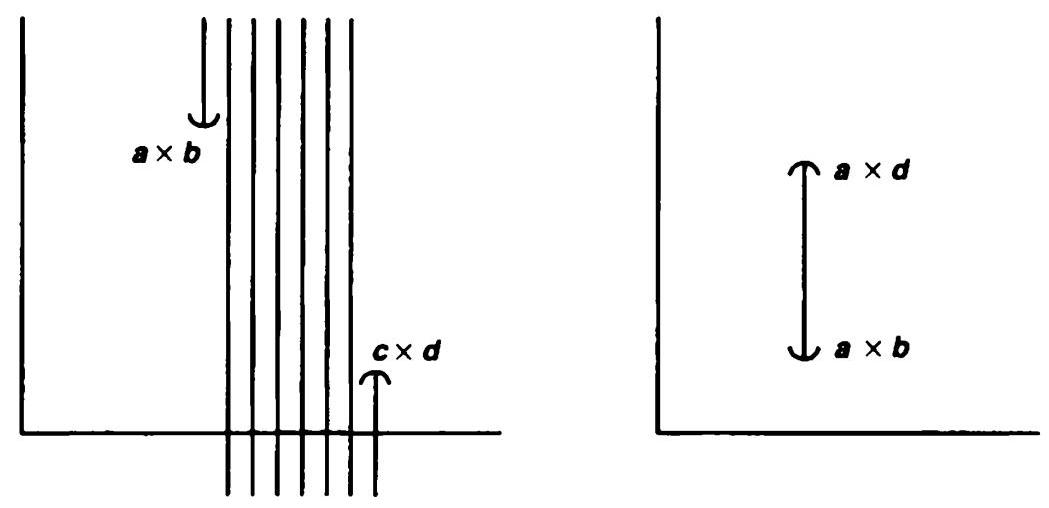
\includegraphics[width=0.9\textwidth]{images/14.1.jpg}
\end{center}
\hspace*{3em}

Figure 14.1
\end{example}
\end{centeredblock}

\begin{centeredblock}
\begin{example}
	The positive integers \({\mathbb{Z}}_{ + }\) form an ordered set with a smallest element. The order topology on \({\mathbb{Z}}_{ + }\) is the discrete topology, for every one-point set is open If \(n > 1\) , then the one-point set \(\{ n\}  = ( {n - 1,n + 1})\) is a basis element; and if \(n = 1\) , the one-point set \(\{ 1\}  = \lbrack 1,2)\) is a basis element.
\end{example}
\end{centeredblock}

\begin{centeredblock}
\begin{example}
	The set \(X = \{ 1,2\}  \times  {\mathbb{Z}}_{ + }\) in the dictionary order is another example of an ordered set with a smallest element Denoting \(1 \times  n\) by \({a}_{n}\) and \(2 \times  n\) by \({b}_{n}\) , we can represent \(X\) by

\[
{a}_{1},{a}_{2},.\;;{b}_{1},{b}_{2},\ldots
\]

The order topology on \(X\) is not the discrete topology. Most one-point sets are open, but there is an exception-the one-point set \(\{  {b}_{1}\}\) . Any open set containing \({b}_{1}\) must contain a basis element about \({b}_{1}\) (by definition), and any basis element containing \({b}_{1}\) contains points of the \({a}_{i}\) sequence.
\end{example}
\end{centeredblock}

\begin{definition}
	If \(X\) is an ordered set, and \(a\) is an element of \(X\) , there are four subsets of \(X\) that are called the rays determined by \(a\) They are the following

\[
( {a, + \infty })  = \{ x \mid  x > a\} ,
\]

\[
( {-\infty ,a})  = \{ x \mid  x < a\} ,
\]

\[
\lbrack a, + \infty ) = \{ x \mid  x \geq  a\} ,
\]

\[
( - \infty ,a\rbrack  = \{ x \mid  x \leq  a\} .
\]

Sets of the first two types are called \index{open ray}, and sets of the last two types are called \index{closed ray}.
\end{definition}

The use of the term ``open'' suggests that \index{Open ray}open rays in \(X\) are open sets in the order topology. And so they are. Consider, for example, the ray \(( {a, + \infty })\) . If \(X\) has a largest element \({b}_{0}\) , then \(( {a, + \infty })\) equals the basis element \(( {a,{b}_{0}}]\) . If \(X\) has no largest element, then \(( {a, + \infty })\) equals the union of all basis elements of the form(a, x), for \(x > a\) . In either case, \(( {a, + \infty })\) is open. A similar argument applies to the ray \(( {-\infty ,a})\) .

The open rays, in fact, form a subbasis for the order topology on \(X\) , as we now show Because the open rays are open in the order topology, the topology they generate is contained in the order topology. On the other hand, every basis element for the order topology equals a finite intersection of open rays; the interval(a, b)equals the intersection of \(( {-\infty ,b})\) and \(( {a, + \infty })\) , while \([  {{a}_{0},b})\) and \(( {a,{b}_{0}}]\) , if they exist, are themselves open rays. Hence the topology generated by the open rays contains the order topology

\section*{§ 15 The Product Topology on \(X \times  Y\)}

If \(X\) and \(Y\) are topological spaces, there is a standard way of defining a topology on the cartesian \index{Product: of continuous maps} product \(X \times  Y\) . We consider this topology now and study some of its properties.

\begin{definition}
	Let \(X\) and \(Y\) be topological spaces. The \index{product topology} on \(X \times  Y\) is the topology having as basis the collection \(\mathcal{B}\) of all sets of the form \(U \times  V\) , where \(U\) is an open subset of \(X\) and \(V\) is an open subset of \(Y\) .
\end{definition}

Let us check that \(\mathcal{B}\) is a basis. The first condition is trivial, since \(X \times  Y\) is itself a basis element. The second condition is almost as easy, since the intersection of any two basis elements \({U}_{1} \times  {V}_{1}\) and \({U}_{2} \times  {V}_{2}\) is another basis element. For

\[
( {{U}_{1} \times  {V}_{1}})  \cap  ( {{U}_{2} \times  {V}_{2}})  = ( {{U}_{1} \cap  {U}_{2}})  \times  ( {{V}_{1} \cap  {V}_{2}})
\]

and the latter set is a basis element because \({U}_{1} \cap  {U}_{2}\) and \({V}_{1} \cap  {V}_{2}\) are open in \(X\) and \(Y\) , respectively. See Figure 15.1.

Note that the collection \(\mathcal{B}\) is not a topology on \(X \times  Y\) . The union of the two rectangles pictured in Figure 15.1, for instance, is not a product of two sets, so it cannot belong to \(\mathcal{B}\) ; however, it is open in \(X \times  Y\) .

Each time we introduce a new concept, we shall try to relate it to the concepts that have been previously introduced. In the present case, we ask: What can one say if the topologies on \(X\) and \(Y\) are given by bases? The answer is as follows:

\begin{theorem}
	If \(\mathcal{B}\) is a basis for the topology of \(X\) and \(\mathcal{C}\) is a basis for the topology of \(Y\) , then the collection

\[
\mathcal{D} = \{ B \times  C \mid  B \in  \mathcal{B}\text{ and }C \in  \mathcal{C}\}
\]

is a basis for the topology of \(X \times  Y\)

\begin{center}
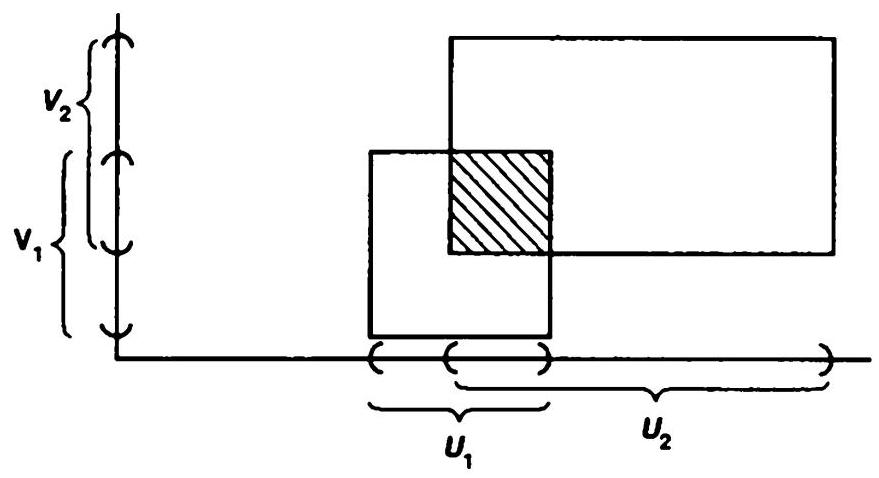
\includegraphics[width=0.8\textwidth]{images/15.1.jpg}
\end{center}
\hspace*{3em} 

Figure 15.1

\end{theorem}
\begin{proof}
We apply Lemma 13.2. Given an open set \(W\) of \(X \times  Y\) and a point \(x \times  y\) of \(W\) , by definition of the \index{Product topology}product topology there is a basis element \(U \times  V\) such that \(x \times  y \in  U \times  V \subset  W\) . Because \(\mathcal{B}\) and \(\mathcal{C}\) are bases for \(X\) and \(Y\) , respectively, we can choose an element \(B\) of \(\mathcal{B}\) such that \(x \in  B \subset  U\) , and an element \(C\) of \(\mathcal{C}\) such that \(y \in  C \subset  V\) . Then \(x \times  y \in  B \times  C \subset  W\) . Thus the collection \(\mathcal{D}\) meets the criterion of Lemma 13.2, so \(\mathcal{D}\) is a basis for \(X \times  Y\) .
\end{proof}

\begin{centeredblock}
\begin{example}
	We have a standard topology on \(\mathbb{R}\) the order topology The product of this topology with itself is called the standard topology on \(\mathbb{R} \times  \mathbb{R} = {\mathbb{R}}^{2}\) . It has as basis the collection of all \index{Quotient map!products}products of open sets of \(\mathbb{R}\) , but the theorem just proved tells us that the much smaller collection of all products \(( {a,b})  \times  ( {c,d})\) of open intervals in \(\mathbb{R}\) will also serve as a basis for the topology of \({\mathbb{R}}^{2}\) Each such set can be pictured as the \index{Int A} interior of a rectangle in \({\mathbb{R}}^{2}\) . Thus the standard topology on \({\mathbb{R}}^{2}\) is just the one we considered in Example 2 of \(§{13}\)
\end{example}
\end{centeredblock}

It is sometimes useful to express the product topology in terms of a subbasis. To do this, we first define certain functions called projections.

\begin{definition}
	Let \({\pi }_{1}.X \times  Y \rightarrow  X\) be defined by the equation

\[
{\pi }_{1}( {x,y})  = x
\]

let \({\pi }_{2} : X \times  Y \rightarrow  Y\) be defined by the equation

\[
{\pi }_{2}( {x,y})  = y
\]

The maps \({\pi }_{1}\) and \({\pi }_{2}\) are called the projections of \(X \times  Y\) onto its first and second factors, respectively.
\end{definition}

We use the word ``onto'' because \({\pi }_{1}\) and \({\pi }_{2}\) are surjective (unless one of the spaces \(X\) or \(Y\) happens to be empty, in which case \(X \times  Y\) is empty and our whole discussion is empty as well!).

If \(U\) is an open subset of \(X\) , then the set \({\pi }_{1}^{-1}( U)\) is precisely the set \(U \times  Y\) , which is open in \(X \times  Y\) . Similarly, if \(V\) is open in \(Y\) , then

\[
{\pi }_{2}^{-1}( V)  = X \times  V
\]

which is also open in \(X \times  Y\) . The intersection of these two sets is the set \(U \times  V\) , as indicated in Figure 15.2. This fact leads to the following theorem:

\begin{theorem}
	The collection

\[
S = \{  {{\pi }_{1}^{-1}( U)  \mid  U\text{ open in }X}\}   \cup  \{  {{\pi }_{2}^{-1}( V)  \mid  V\text{ open in }Y}\}
\]

is a subbasis for the product topology on \(X \times  Y\) .

\begin{center}
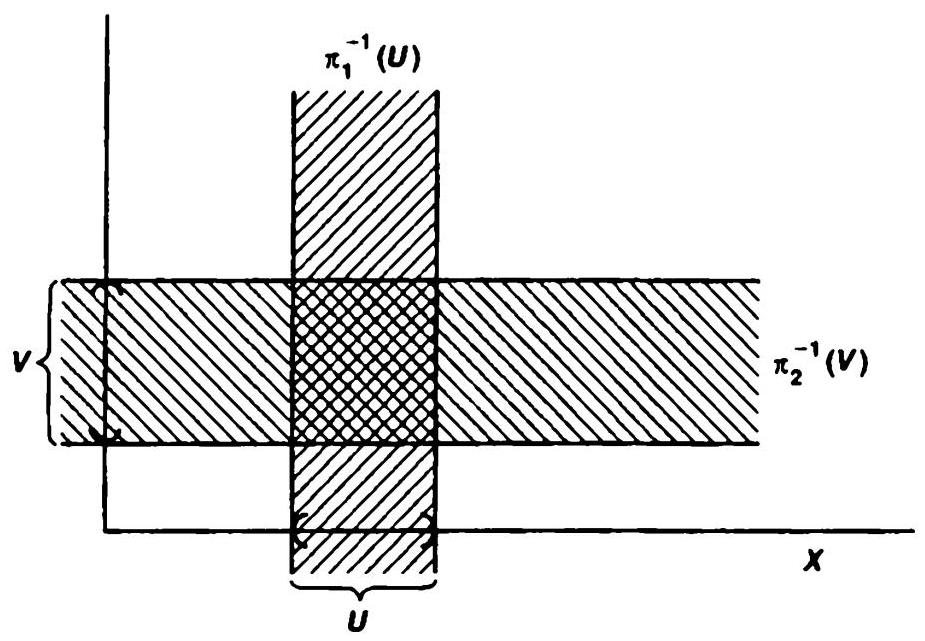
\includegraphics[width=0.8\textwidth]{images/15.2.jpg}
\end{center}
\hspace*{3em} 

Figure 15.2

\end{theorem}
\begin{proof}
Let \(\mathcal{T}\) denote the product topology on \(X \times  Y\) , let \({\mathcal{T}}^{\prime }\) be the topology generated by \(S\) . Because every element of \(S\) belongs to \(\mathcal{T}\) , so do arbitrary unions of finite intersections of elements of \(S\) . Thus \({\mathcal{T}}^{\prime } \subset  \mathcal{T}\) . On the other hand, every basis element \(U \times  V\) for the topology \(\mathcal{T}\) is a finite intersection of elements of \(S\) , since

\[
U \times  V = {\pi }_{1}^{-1}( U)  \cap  {\pi }_{2}^{-1}( V)
\]

Therefore, \(U \times  V\) belongs to \({\mathcal{T}}^{\prime }\) , so that \(\mathcal{T} \subset  {\mathcal{T}}^{\prime }\) as well
\end{proof}

\section*{§ 16 The Subspace Topology}

\index{Subspace Topology}
\begin{definition}
	Let \(X\) be a topological space with topology \(\mathcal{T}\) . If \(Y\) is a subset of \(X\) , the collection

\[
{\mathcal{T}}_{Y} = \{ Y \cap  U \mid  U \in  \mathcal{T}\}
\]

is a topology on \(Y\) , called the \index{Subspace topology}subspace topology. With this topology, \(Y\) is called a subspace of \(X\) ; its open sets consist of all intersections of open sets of \(X\) with \(Y\) .
\end{definition}

It is easy to see that \({\mathcal{T}}_{Y}\) is a topology. It contains \(\varnothing\) and \(Y\) because

\[
\varnothing  = Y \cap  \varnothing \;\text{ and }\;Y = Y \cap  X,
\]

where \(\varnothing\) and \(X\) are elements of \(\mathcal{T}\) . The fact that it is closed under finite intersections and arbitrary unions follows from the equations

\[
( {{U}_{1} \cap  Y})  \cap  \cdots  \cap  ( {{U}_{n} \cap  Y})  = ( {{U}_{1} \cap  \cdots  \cap  {U}_{n}})  \cap  Y
\]

\[
\mathop{\bigcup }\limits_{{\alpha  \in  J}}( {{U}_{\alpha } \cap  Y})  = ( {\mathop{\bigcup }\limits_{{\alpha  \in  J}}{U}_{\alpha }})  \cap  Y
\]

\begin{lemma}
	If \(\mathcal{B}\) is a basis for the topology of \(X\) then the collection

\[
{\mathcal{B}}_{Y} = \{ B \cap  Y \mid  B \in  \mathcal{B}\}
\]

is a basis for the subspace topology on \(Y\) .
\end{lemma}

\begin{proof}
Given \(U\) open in \(X\) and given \(y \in  U \cap  Y\) , we can choose an element \(B\) of \(\mathcal{B}\) such that \(y \in  B \subset  U\) . Then \(y \in  B \cap  Y \subset  U \cap  Y\) . It follows from Lemma 13.2 that \({\mathcal{B}}_{Y}\) is a basis for the subspace topology on \(Y\) .

When dealing with a space \(X\) and a subspace \(Y\) , one needs to be careful when one uses the term ``open set''. Does one mean an element of the topology of \(Y\) or an element of the topology of \(X\) ? We make the following definition : If \(Y\) is a subspace of \(X\) , we say that a set \(U\) is open in \(Y\) (or open relative to \(Y\) ) if it belongs to the topology of \(Y\) ; this implies in particular that it is a subset of \(Y\) . We say that \(U\) is open in \(X\) if it belongs to the topology of \(X\)

There is a special situation in which every set open in \(Y\) is also open in \(\mathbf{X}\) .
\end{proof}

\begin{lemma}
	Let \(Y\) be a subspace of \(X\) . If \(U\) is open in \(Y\) and \(Y\) is open in \(X\) , then \(U\) is open in \(X\) .
\end{lemma}

\begin{proof}
Since \(U\) is open in \(Y,U = Y \cap  V\) for some set \(V\) open in \(X\) . Since \(Y\) and \(V\) are both open in \(X\) , so is \(Y \cap  V\)

Now let us explore the relation between the subspace topology and the order and product topologies For product topologies, the result is what one might expect; for order topologies, it is not.
\end{proof}

\begin{theorem}
	If \(A\) is a subspace of \(X\) and \(B\) is a subspace of \(Y\) , then the product topology on \(A \times  B\) is the same as the topology \(A \times  B\) inherits as a subspace of \(X \times  Y\) .

\end{theorem}
\begin{proof}
The set \(U \times  V\) is the general basis element for \(X \times  Y\) , where \(U\) is open in \(X\) and \(V\) is open in \(Y\) . Therefore, \(( {U \times  V})  \cap  ( {A \times  B})\) is the general basis element for the subspace topology on \(A \times  B\) . Now

\[
( {U \times  V})  \cap  ( {A \times  B})  = ( {U \cap  A})  \times  ( {V \cap  B}) .
\]

Since \(U \cap  A\) and \(V \cap  B\) are the general open sets for the subspace topologies on \(A\) and \(B\) , respectively, the set \(( {U \cap  A})  \times  ( {V \cap  B})\) is the general basis element for the product topology on \(A \times  B\) .

The conclusion we draw is that the bases for the subspace topology on \(A \times  B\) and for the product topology on \(A \times  B\) are the same. Hence the topologies are the same. ∎

Now let \(X\) be an ordered set in the order topology, and let \(Y\) be a subset of \(X\) . The order relation on \(X\) , when restricted to \(Y\) , makes \(Y\) into an ordered set. However, the resulting order topology on \(Y\) need not be the same as the topology that \(Y\) inherits as a subspace of \(X\) . We give one example where the subspace and order topologies on \(Y\) agree, and two examples where they do not.
\end{proof}

\begin{centeredblock}
\begin{example}
	Consider the subset \(Y = [  {0,1}]\) of the real line \(\mathbb{R}\) , in the subspace topology. The subspace topology has as basis all sets of the form \(( {a,b})  \cap  Y\) , where(a, b)is an open interval in \(\mathbb{R}\) Such a set is of one of the following types.

\[
( {a,b})  \cap  Y = \{ \begin{array}{ll} ( {a,b}) & \text{ if }a\text{ and }b\text{ are in }Y, \\  \lbrack 0,b) & \text{ if only }b\text{ is in }Y, \\  ( {a,1}) & \text{ if only }a\text{ is in }Y, \\  Y\text{ or }\varnothing & \text{ if neither }a\text{ nor }b\text{ is in }Y. \end{array}.
\]

By definition, each of these sets is open in \(Y\) But sets of the second and third types are not open in the larger space \(\mathbb{R}\) .

Note that these sets form a basis for the order topology on \(Y\) Thus, we see that in the case of the set \(Y = [  {0,1}]\) , its subspace topology (as a subspace of \(\mathbb{R}\) ) and its order topology are the same.
\end{example}
\end{centeredblock}

\begin{centeredblock}
\begin{example}
	Let \(Y\) be the subset \(\lbrack 0,1) \cup  \{ 2\}\) of \(\mathbb{R}\) . In the subspace topology on \(Y\) the one-point set \(\{ 2\}\) is open, because it is the intersection of the open set \(( {\frac{3}{2},\frac{5}{2}})\) with \(Y\) But in the order topology on \(Y\) , the set \(\{ 2\}\) is not open. Any basis element for the order topology on \(Y\) that contains 2 is of the form

\[
\{ x \mid  x \in  Y\text{ and }a < x \leq  2\}
\]

for some \(a \in  Y\) , such a set necessarily contains points of \(Y\) less than 2
\end{example}
\end{centeredblock}

\begin{centeredblock}
\begin{example}
	Let \(I = [  {0,1}]\) The dictionary order on \(I \times  I\) is just the restriction to \(I \times  I\) of the dictionary order on the plane \(\mathbb{R} \times  \mathbb{R}\) . However, the dictionary order topology on \(I \times  I\) is not the same as the subspace topology on \(I \times  I\) obtained from the dictionary order topology on \(\mathbb{R} \times  {\mathbb{R}}^{1}\) For example, the set \(\{ 1/2\}  \times  (1/2,1\rbrack\) is open in \(I \times  I\) in the subspace topology, but not in the order topology, as you can check. See Figure 16.1.
\end{example}
\end{centeredblock}

The set \(I \times  I\) in the dictionary order topology will be called the ordered \index{Square metric (see also )} square, and denoted by \(\index{I@\({I}_{o}^{2}\)} {I}_{o}^{2}\) .

The anomaly illustrated in Examples 2 and 3 does not occur for intervals or rays in an ordered set \(X\) . This we now prove.

Given an ordered set \(X\) , let us say that a subset \(Y\) of \(X\) is \index{Convex set: in an ordered set} convex in \(X\) if for each pair of points \(a < b\) of \(Y\) , the entire interval(a, b)of points of \(X\) lies in \(Y\) . Note that intervals and rays in \(X\) are convex in \(X\) .

\begin{center}
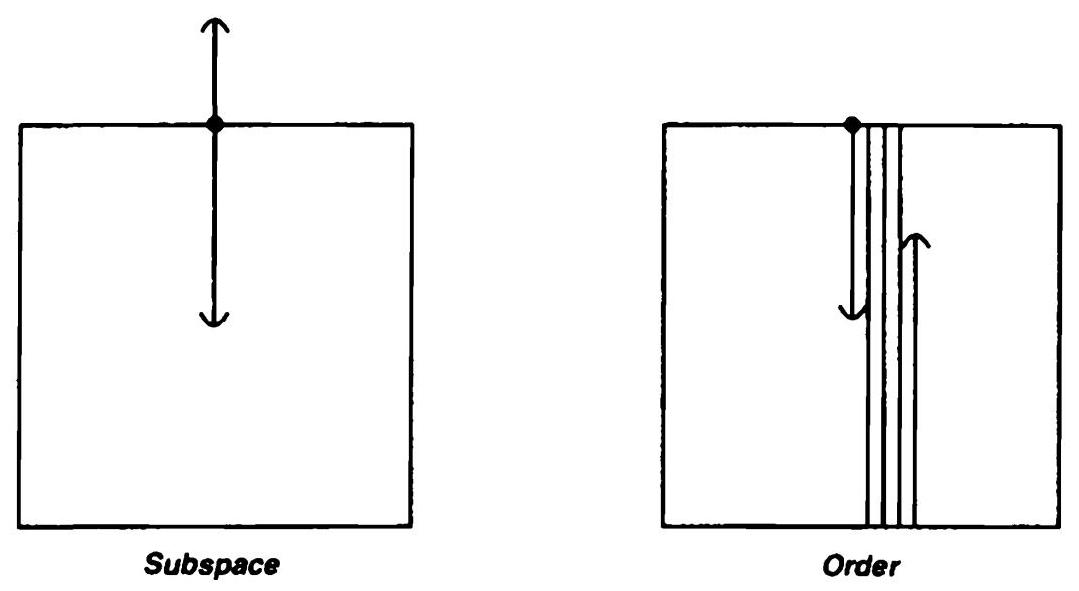
\includegraphics[width=1.0\textwidth]{images/16.1.jpg}
\end{center}
\hspace*{3em} 

Figure 16.1

\begin{theorem}
	Let \(X\) be an ordered set in the order topology; let \(Y\) be a subset of \(X\) that is convex in \(X\) Then the order topology on \(Y\) is the same as the topology \(Y\) inherits as a subspace of \(X\) .

\end{theorem}
\begin{proof}
Consider the ray \(( {a, + \infty })\) in \(X\) . What is its intersection with \(Y\) ? If \(a \in  Y\) , then

\[
( {a, + \infty })  \cap  Y = \{ x \mid  x \in  Y\text{ and }x > a\} ;
\]

this is an open ray of the ordered set \(Y\) . If \(a \notin  Y\) , then \(a\) is either a lower bound on \(Y\) or an upper bound on \(Y\) , since \(Y\) is convex. In the former case, the set \(( {a, + \infty })  \cap  Y\) equals all of \(Y\) ; in the latter case, it is empty.

A similar remark shows that the intersection of the ray \(( {-\infty ,a})\) with \(Y\) is either an open ray of \(Y\) , or \(Y\) itself, or empty. Since the sets \(( {a, + \infty })  \cap  Y\) and \(( {-\infty ,a})  \cap  Y\) form a subbasis for the subspace topology on \(Y\) , and since each is open in the order topology, the order topology contains the subspace topology.

To prove the reverse, note that any open ray of \(Y\) equals the intersection of an open ray of \(X\) with \(Y\) , so it is open in the subspace topology on \(Y\) . Since the open rays of \(Y\) are a subbasis for the order topology on \(Y\) , this topology is contained in the subspace topology.

To avoid ambiguity, let us agree that whenever \(X\) is an ordered set in the order topology and \(Y\) is a subset of \(X\) , we shall assume that \(Y\) is given the subspace topology unless we specifically state otherwise. If \(Y\) is convex in \(X\) , this is the same as the order topology on \(Y\) , otherwise, it may not be.
\end{proof}

\section*{Exercises}
\begin{enumerate}[itemsep=0.4em, parsep=0pt, topsep=0pt, partopsep=0pt, leftmargin=*, label=\arabic*., ref=\arabic*]
\item Show that if \(Y\) is a subspace of \(X\) , and \(A\) is a subset of \(Y\) , then the topology \(A\) inherits as a subspace of \(Y\) is the same as the topology it inherits as a subspace of \(X\) .
\item If \(\mathcal{T}\) and \({\mathcal{T}}^{\prime }\) are topologies on \(X\) and \({\mathcal{T}}^{\prime }\) is strictly finer than \(\mathcal{T}\) , what can you say about the corresponding subspace topologies on the subset \(Y\) of \(X\) ?
\item Consider the set \(Y = \{  - 1,1\}\) as a subspace of \(\mathbb{R}\) . Which of the following sets are open in \(Y\) ? Which are open in \(\mathbb{R}\) ? \[ A = \{  {x| {\frac{1}{2} < }| x \mid   < 1}\}  , \] \[ B = \{  {x| {\frac{1}{2} < }| x \mid   \leq  1}\}  , \] \[ C = \{  {x| {\frac{1}{2} \leq  }| x \mid   < 1}\}  , \] \[ D = \{  {x| {\frac{1}{2} \leq  }| x \mid   \leq  1}\}  \text{ , } \] \[ E = \{  {x| {0 < }| x \mid   < 1\text{ and }1/x \notin  {\mathbb{Z}}_{ + }}\}  . \]
\item A map \(f : X \rightarrow  Y\) is said to be an \index{open map} if for every open set \(U\) of \(X\) , the set \(f( U)\) is open in \(Y\) . Show that \({\pi }_{1} : X \times  Y \rightarrow  X\) and \({\pi }_{2} : X \times  Y \rightarrow  Y\) are \index{Open map}open maps.
\item Let \(X\) and \({X}^{\prime }\) denote a single set in the topologies \(\mathcal{T}\) and \({\mathcal{T}}^{\prime }\) , respectively; let \(Y\) and \({Y}^{\prime }\) denote a single set in the topologies \(\mathcal{U}\) and \({\mathcal{U}}^{\prime }\) , respectively. Assume these sets are nonempty.
  \begin{enumerate}[itemsep=0.2em, parsep=0pt, topsep=0pt, partopsep=0pt, leftmargin=*, label=(\alph*), align=left]
  \item Show that if \({\mathcal{T}}^{\prime } \supset  \mathcal{T}\) and \({\mathcal{U}}^{\prime } \supset  \mathcal{U}\) , then the product topology on \({X}^{\prime } \times  {Y}^{\prime }\) is finer than the product topology on \(X \times  Y\) .
  \item Does the converse of (a) hold? Justify your answer.
  \end{enumerate}
\item Show that the countable collection \[ \{ ( {a,b})  \times  ( {\mathrm{c},d})  \mid  a < b\text{ and }\mathrm{c} < d\text{ , and }a,b,\mathrm{c},d\text{ are rational }\} \] is a basis for \({\mathbb{R}}^{2}\) .
\item Let \(X\) be an ordered set. If \(Y\) is a proper subset of \(X\) that is convex in \(X\) , does it follow that \(Y\) is an interval or a ray in \({X}^{\gamma }\)
\item If \(L\) is a straight line in the plane, describe the topology \(L\) inherits as a subspace of \({\mathbb{R}}_{\ell } \times  \mathbb{R}\) and as a subspace of \({\mathbb{R}}_{\ell } \times  {\mathbb{R}}_{\ell }\) . In each case it is a familiar topology.
\item Show that the dictionary order topology on the set \(\mathbb{R} \times  \mathbb{R}\) is the same as the product topology \({\mathbb{R}}_{d} \times  \mathbb{R}\) , where \({\mathbb{R}}_{d}\) denotes \(\mathbb{R}\) in the discrete topology. Compare this topology with the standard topology on \({\mathbb{R}}^{2}\) .
\item Let \(I = [  {0,1}]\) . Compare the product topology on \(I \times  I\) , the dictionary order topology on \(I \times  I\) , and the topology \(I \times  I\) inherits as a subspace of \(\mathbb{R} \times  \mathbb{R}\) in the dictionary order topology.
\end{enumerate}
\section*{§ 17 Closed Sets and Limit Points}

Now that we have a few examples at hand, we can introduce some of the basic concepts associated with topological spaces. In this section, we treat the notions of closed set, \index{Closure (cont.)} closure of a set, and limit point. These lead naturally to consideration of a certain axiom for topological spaces called the Hausdorff axiom.

\section*{Closed Sets}

A subset \(A\) of a topological space \(X\) is said to be closed if the set \(X - A\) is open.

\begin{centeredblock}
\begin{example}
	The subset \([  {a,b}]\) of \(\mathbb{R}\) is closed because its complement

\[
\mathbb{R} - [  {a,b}]   = ( {-\infty ,a})  \cup  ( {b, + \infty }) ,
\]

is open. Similarly, \(\lbrack a, + \infty )\) is closed, because its complement \(( {-\infty ,a})\) is open. These facts justify our use of the terms ``\index{Closed interval}closed interval'' and ``\index{Closed ray}closed ray'' The subset \(\lbrack a,b)\) of \(\mathbb{R}\) is neither open nor closed.
\end{example}
\end{centeredblock}

\begin{centeredblock}
\begin{example}
	In the plane \({\mathbb{R}}^{2}\) , the set

\[
\{ x \times  y \mid  x \geq  0\text{ and }y \geq  0\}
\]

is closed, because its complement is the union of the two sets

\[
( {-\infty ,0})  \times  \mathbb{R}\;\text{ and }\;\mathbb{R} \times  ( {-\infty ,0}) ,
\]

each of which is a product of open sets of \(\mathbb{R}\) and is, therefore, open in \({\mathbb{R}}^{2}\)
\end{example}
\end{centeredblock}

\begin{centeredblock}
\begin{example}
	In the finite complement topology on a set \(X\) , the closed sets consist of \(X\) itself and all finute subsets of \(X\)
\end{example}
\end{centeredblock}

\begin{centeredblock}
\begin{example}
	In the discrete topology on the set \(X\) , every set is open, it follows that every set is closed as well.
\end{example}
\end{centeredblock}

\begin{centeredblock}
\begin{example}
	Consider the following subset of the real line:

\[
Y = [  {0,1}]   \cup  ( {2,3}) \text{ , }
\]

in the subspace topology. In this space, the set \([  {0,1}]\) is open, since it is the intersection of the open set \(( {-\frac{1}{2},\frac{3}{2}})\) of \(\mathbb{R}\) with \(Y\) Similarly,(2,3)is open as a subset of \(Y\) ; it is even open as a subset of \(\mathbb{R}\) . Since \([  {0,1}]\) and(2,3)are complements in \(Y\) of each other, we conclude that both \([  {0,1}]\) and(2,3)are closed as subsets of \(Y\)
\end{example}
\end{centeredblock}

These examples suggest that an answer to the mathematician's riddle: ``How is a set different from a door?'' should be: ``A door must be either open or closed, and cannot be both, while a set can be open, or closed, or both, or neither!''

The collection of closed subsets of a space \(X\) has properties similar to those satisfied by the collection of open subsets of \(X\) :

\begin{theorem}
	Let \(X\) be a topological space. Then the following conditions hold:

(1) \(\varnothing\) and \(X\) are closed.

(2) Arbitrary intersections of closed sets are closed.

(3) Finite unions of closed sets are closed.

\end{theorem}
\begin{proof}
(1) \(\varnothing\) and \(X\) are closed because they are the complements of the open sets \(X\) and \(\varnothing\) , respectively.

(2) Given a collection of closed sets \({\{  {A}_{\alpha }\}  }_{\alpha  \in  J}\) , we apply DeMorgan's law,

\[
X - \mathop{\bigcap }\limits_{{\alpha  \in  J}}{A}_{\alpha } = \mathop{\bigcup }\limits_{{\alpha  \in  J}}( {X - {A}_{\alpha }})
\]

Since the sets \(X - {A}_{\alpha }\) are open by definition, the right side of this equation represents an arbitrary union of open sets, and is thus open. Therefore, \(\cap  {A}_{\alpha }\) is closed.

(3) Similarly, if \({A}_{i}\) is closed for \(i = 1,\ldots ,n\) , consider the equation

\[
X - \mathop{\bigcup }\limits_{{i = 1}}^{n}{A}_{i} = \mathop{\bigcap }\limits_{{i = 1}}^{n}( {X - {A}_{i}})
\]

The set on the right side of this equation is a finite intersection of open sets and is therefore open. Hence \(\bigcup {A}_{i}\) is closed.

Instead of using open sets, one could just as well specify a topology on a space by giving a collection of sets (to be called ``\index{Closed set}closed sets'') satisfying the three properties of this theorem. One could then define open sets as the complements of closed sets and proceed just as before. This procedure has no particular advantage over the one we have adopted, and most mathematicians prefer to use open sets to define topologies.

Now when dealing with subspaces, one needs to be careful in using the term ``closed set.'' If \(Y\) is a subspace of \(X\) , we say that a set \(A\) is closed in \(Y\) if \(A\) is a subset of \(Y\) and if \(A\) is closed in the subspace topology of \(Y\) (that is, if \(Y - A\) is open in \(Y\) ). We have the following theorem:
\end{proof}

\begin{theorem}
	Let \(Y\) be a subspace of \(X\) . Then a set \(A\) is closed in \(Y\) if and only if it equals the intersection of a closed set of \(X\) with \(Y\) .

\end{theorem}
\begin{proof}
Assume that \(A = C \cap  Y\) , where \(C\) is closed in \(X\) . (See Figure 17.1.) Then \(X - C\) is open in \(X\) , so that \(( {X - C})  \cap  Y\) is open in \(Y\) , by definition of the subspace topology. But \(( {X - C})  \cap  Y = Y - A\) . Hence \(Y - A\) is open in \(Y\) , so that \(A\) is closed in \(Y\) . Conversely, assume that \(A\) is closed in \(Y\) . (See Figure 17.2.) Then \(Y - A\) is open in \(Y\) , so that by definition it equals the intersection of an open set \(U\) of \(X\) with \(Y\) The set \(X - U\) is closed in \(X\) , and \(A = Y \cap  ( {X - U})\) , so that \(A\) equals the intersection of a closed set of \(X\) with \(Y\) , as desired.

A set \(A\) that is closed in the subspace \(Y\) may or may not be closed in the larger space \(X\) . As was the case with open sets, there is a criterion for \(A\) to be closed in \(X\) ; we leave the proof to you.

\begin{center}
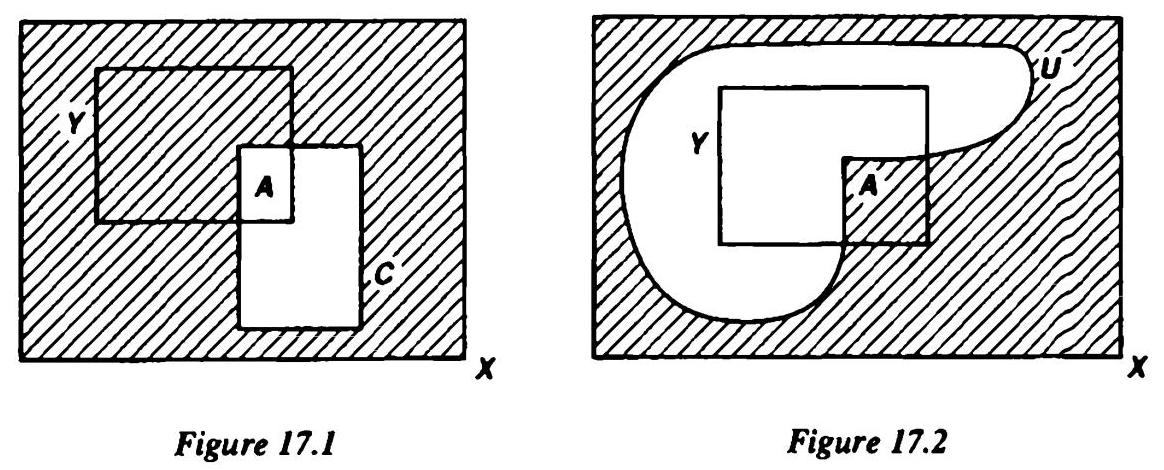
\includegraphics[width=1.0\textwidth]{images/17.1.jpg}
\end{center}
\hspace*{3em} 
\end{proof}

\begin{theorem}
	Let \(Y\) be a subspace of \(X\) . If \(A\) is closed in \(Y\) and \(Y\) is closed in \(X\) , then \(A\) is closed in \(X\) .

\end{theorem}
\section*{Closure and Interior of a Set}

Given a subset \(A\) of a topological space \(X\) , the interior of \(A\) is defined as the union of all open sets contained in \(A\) , and the closure of \(A\) is defined as the intersection of all closed sets containing \(A\) .

The interior of \(A\) is denoted by Int \(A\) and the closure of \(A\) is denoted by \(\mathrm{{Cl}}A\) or by \(\index{A@\(\bar{A}\)}\) . Obviously Int \(A\) is an open set and \(\bar{A}\) is a closed set; furthermore,

\[
\operatorname{Int}A \subset  A \subset  \bar{A}.
\]

If \(A\) is open, \(A = \operatorname{Int}A\) ; while if \(A\) is closed, \(A = \bar{A}\) .

We shall not make much use of the interior of a set, but the \index{Closure}closure of a set will be quite important.

When dealing with a topological space \(X\) and a subspace \(Y\) , one needs to exercise care in taking closures of sets If \(A\) is a subset of \(Y\) , the closure of \(A\) in \(Y\) and the closure of \(A\) in \(X\) will in general be different In such a situation, we reserve the notation \(\bar{A}\) to stand for the closure of \(A\) in \(X\) . The closure of \(A\) in \(Y\) can be expressed in terms of \(\bar{A}\) , as the following theorem shows:

\begin{theorem}
	Let \(Y\) be a subspace of \(X\) , let \(A\) be a subset of \(Y\) , let \(\bar{A}\) denote the closure of \(A\) in \(X\) . Then the closure of \(A\) in \(Y\) equals \(\bar{A} \cap  Y\) .

\end{theorem}
\begin{proof}
Let \(B\) denote the closure of \(A\) in \(Y\) . The set \(\bar{A}\) is closed in \(X\) , so \(\bar{A} \cap  Y\) is closed in \(Y\) by Theorem 17.2. Since \(\bar{A} \cap  Y\) contains \(A\) , and since by definition \(B\) equals the intersection of all closed subsets of \(Y\) containing \(A\) , we must have \(B \subset  ( {\bar{A} \cap  Y})\) .

On the other hand, we know that \(B\) is closed in \(Y\) . Hence by Theorem 17.2, \(B = C \cap  Y\) for some set \(C\) closed in \(X\) . Then \(C\) is a closed set of \(X\) containing \(A\) ; because \(\bar{A}\) is the intersection of all such closed sets, we conclude that \(\bar{A} \subset  C\) . Then \(( {\bar{A} \cap  Y})  \subset  ( {C \cap  Y})  = B.\)

The definition of the closure of a set does not give us a convenient way for actually finding the closures of specific sets, since the collection of all closed sets in \(X\) , like the collection of all open sets, is usually much too big to work with. Another way of describing the closure of a set, useful because it involves only a basis for the topology of \(X\) , is given in the following theorem.

First let us introduce some convenient terminology. We shall say that a set \(A\) intersects a set \(B\) if the intersection \(A \cap  B\) is not empty.
\end{proof}

\begin{theorem}
	Let \(A\) be a subset of the topological space \(X\) .

(a) Then \(x \in  \bar{A}\) if and only if every open set \(U\) containing \(x\) intersects \(A\) .

(b) Supposing the topology of \(X\) is given by a basis, then \(x \in  \bar{A}\) if and only if every basis element \(B\) containing \(x\) intersects \(A\) .

\end{theorem}
\begin{proof}
Consider the statement in (a). It is a statement of the form \(P \Leftrightarrow  Q\) . Let us transform each implication to its contrapositive, thereby obtaining the logically equivalent statement (not \(P\) ) \(\Leftrightarrow\) (not \(Q\) ). Written out, it is the following.

\(x \notin  \bar{A} \Leftrightarrow\) there exists an open set \(U\) containing \(x\) that does not intersect \(A\) .

In this form, our theorem is easy to prove. If \(x\) is not in \(\bar{A}\) , the set \(U = X - \bar{A}\) is an open set containing \(x\) that does not intersect \(A\) , as desired Conversely, if there exists an open set \(U\) containing \(x\) which does not intersect \(A\) , then \(X - U\) is a closed set containing \(A\) By definition of the closure \(\bar{A}\) , the set \(X - U\) must contain \(\bar{A}\) , therefore, \(x\) cannot be in \(\bar{A}\) .

Statement (b) follows readily If every open set containing \(x\) intersects \(A\) , so does every basis element \(B\) containing \(x\) , because \(B\) is an open set. Conversely, if every basis element containing \(x\) intersects \(A\) , so does every open set \(U\) containing \(x\) , because \(U\) contains a basis element that contains \(x\) .

Mathematicians often use some special terminology here. They shorten the statement `` \(U\) is an open set containing \(x\) `` to the phrase

\[
\text{ " }U\text{ is a neighborhood of }x\text{ ." }
\]

Using this terminology, one can write the first half of the preceding theorem as follows:

If \(A\) is a subset of the topological space \(X\) , then \(x \in  \widehat{A}\) if and only if every \index{neighborhood} of \(x\) intersects \(A\) .
\end{proof}

\begin{centeredblock}
\begin{example}
	Let \(X\) be the real line \(\mathbb{R}\) . If \(A = (0,1\rbrack\) , then \(\bar{A} = [  {0,1}]\) , for every \index{Neighborhood}neighborhood of 0 intersects \(A\) , while every point outside \([  {0,1}]\) has a neighborhood disjoint from \(A\) Similar arguments apply to the following subsets of \(X\)

If \(B = \{  {1/n \mid  n \in  {\mathbb{Z}}_{ + }}\}\) , then \(\bar{B} = \{ 0\}  \cup  B\) If \(C = \{ 0\}  \cup  ( {1,2})\) , then \(\bar{C} = \{ 0\}  \cup  [  {1,2}]\) If \(\mathbb{Q}\) is the set of rational numbers, then \(\widehat{\mathbb{Q}} = \mathbb{R}\) If \({\mathbb{Z}}_{ + }\) is the set of positive integers, then \({\overline{\mathbb{Z}}}_{ + } = {\mathbb{Z}}_{ + }\) . If \({\mathbb{R}}_{ + }\) is the set of positive reals, then the closure of \({\mathbb{R}}_{ + }\) is the set \({\mathbb{R}}_{ + } \cup  \{ 0\}\) . (This is the reason we introduced the notation \({\overline{\mathbb{R}}}_{ + }\) for the set \({\mathbb{R}}_{ + } \cup  \{ 0\}\) , back in \(\$ 2\) )
\end{example}
\end{centeredblock}

\begin{centeredblock}
\begin{example}
	Consider the subspace \(Y = (0,1\rbrack\) of the real line \(\mathbb{R}\) . The set \(A = ( {0,\frac{1}{2}})\) is a subset of \(Y\) , its closure in \(\mathbb{R}\) is the set \([  {0,\frac{1}{2}}]\) , and its closure in \(Y\) is the set \([  {0,\frac{1}{2}}]   \cap  Y =\)  \(( {0,\frac{1}{2}}]\)
\end{example}
\end{centeredblock}

Some mathematicians use the term ``neighborhood'' differently. They say that \(A\) is a neighborhood of \(x\) if \(A\) merely contains an open set containing \(x\) . We shall not follow this practice.

\section*{Limit Points}

There is yet another way of describing the closure of a set, a way that involves the important concept of limit point, which we consider now.

If \(A\) is a subset of the topological space \(X\) and if \(x\) is a point of \(X\) , we say that \(x\) is a limit point (or ``cluster point,'' or ``point of accumulation'') of \(A\) if every neighborhood of \(x\) intersects \(A\) in some point other than \(x\) itself. Said differently, \(x\) is a limit point of \(A\) if it belongs to the closure of \(A - \{ x\}\) The point \(x\) may lie in \(A\) or not; for this definition it does not matter.

\begin{centeredblock}
\begin{example}
	Consider the real line \(\mathbb{R}\) . If \(A = (0,1\rbrack\) , then the point 0 is a limit point of \(A\) and so is the point \(\frac{1}{2}\) . In fact, every point of the interval \([  {0,1}]\) is a \index{Limit point}limit point of \(A\) , but no other point of \(\mathbb{R}\) is a limit point of \(A\)

If \(B = \{  {1/n \mid  n \in  {\mathbb{Z}}_{ + }}\}\) , then 0 is the only limit point of \(B\) . Every other point \(x\) of \(\mathbb{R}\) has a neighborhood that either does not intersect \(B\) at all, or it intersects \(B\) only in the point \(x\) itself. If \(C = \{ 0\}  \cup  ( {1,2})\) , then the limit points of \(C\) are the points of the interval \([  {1,2}]\) . If \(\mathbb{Q}\) is the set of rational numbers, every point of \(\mathbb{R}\) is a limit point of \(\mathbb{Q}\) . If \({\mathbb{Z}}_{ + }\) is the set of positive integers, no point of \(\mathbb{R}\) is a limit point of \({\mathbb{Z}}_{ + }\) . If \({\mathbb{R}}_{ + }\) is the set of positive reals, then every point of \(\{ 0\}  \cup  {\mathbb{R}}_{ + }\) is a limit point of \({\mathbb{R}}_{ + }\)
\end{example}
\end{centeredblock}

\index{Comparison test for infinite series} Comparison of Examples 6 and 8 suggests a relationship between the closure of a set and the limit points of a set. That relationship is given in the following theorem:

\begin{theorem}
	Let \(A\) be a subset of the topological space \(X\) , let \({A}^{\prime }\) be the set of all limit points of \(A\) . Then

\[
\bar{A} = A \cup  {A}^{\prime }.
\]

\end{theorem}
\begin{proof}
If \(x\) is in \({A}^{\prime }\) , every neighborhood of \(x\) intersects \(A\) (in a point different from \(x\) ). Therefore, by Theorem 17.5, \(x\) belongs to \(\bar{A}\) Hence \({A}^{\prime } \subset  \bar{A}\) . Since by definition \(A \subset  \bar{A}\) , it follows that \(A \cup  {A}^{\prime } \subset  \bar{A}\) .

To demonstrate the reverse inclusion, we let \(x\) be a point of \(\bar{A}\) and show that \(x \in  A \cup  {A}^{\prime }\) . If \(x\) happens to lie in \(A\) , it is trivial that \(x \in  A \cup  {A}^{\prime }\) ; suppose that \(x\) does not lie in \(A\) . Since \(x \in  \bar{A}\) , we know that every neighborhood \(U\) of \(x\) intersects \(A\) ; because \(x \notin  A\) , the set \(U\) must intersect \(A\) in a point different from \(x\) . Then \(x \in  {A}^{\prime }\) , so that \(x \in  A \cup  {A}^{\prime }\) , as desired.
\end{proof}

\begin{corollary}
	A subset of a topological space is closed if and only if it contains all its limit points.
\end{corollary}

Proof The set \(A\) is closed if and only if \(A = \bar{A}\) , and the latter holds if and only if \({A}^{\prime } \subset  A\) .

\section*{Hausdorff Spaces}

One's experience with open and closed sets and limit points in the real line and the plane can be misleading when one considers more general topological spaces. For example, in the spaces \(\mathbb{R}\) and \({\mathbb{R}}^{2}\) , each one-point set \(\{  {x}_{0}\}\) is closed. This fact is easily proved; every point different from \({x}_{0}\) has a neighborhood not intersecting \(\{  {x}_{0}\}\) , so that \(\{  {x}_{0}\}\) is its own closure. But this fact is not true for arbitrary topological spaces. Consider the topology on the three-point set \(\{ a,b,c\}\) indicated in Figure 17.3. In this space, the one-point set \(\{ b\}\) is not closed, for its complement is not open.

\begin{center}
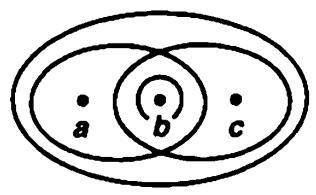
\includegraphics[width=0.2\textwidth]{images/17.3.jpg}
\end{center}
\hspace*{3em} 

Figure 17.3

Similarly, one's experience with the properties of \index{convergent sequence} in \(\mathbb{R}\) and \({\mathbb{R}}^{2}\) can be misleading when one deals with more general topological spaces. In an arbitrary topological space, one says that a sequence \({x}_{1},{x}_{2},\ldots\) of points of the space \(X\) converges to the point \(x\) of \(X\) provided that, corresponding to each neighborhood \(U\) of \(x\) , there is a positive integer \(N\) such that \({x}_{n} \in  U\) for all \(n \geq  N\) . In \(\mathbb{R}\) and \({\mathbb{R}}^{2}\) , a sequence cannot converge to more than one point, but in an arbitrary space, it can. In the space indicated in Figure 17.3, for example, the sequence defined by setting \({x}_{n} = b\) for all \(n\) converges not only to the point \(b\) , but also to the point \(a\) and to the point \(c\) !

Topologies in which one-point sets are not closed, or in which sequences can converge to more than one point, are considered by many mathematicians to be somewhat strange. They are not really very interesting, for they seldom occur in other branches of mathematics And the theorems that one can prove about topological spaces are rather limited if such examples are allowed. Therefore, one often imposes an additional condition that will rule out examples like this one, bringing the class of spaces under consideration closer to those to which one's geo\index{Metric}metric intuition applies. The condition was suggested by the mathematician Felix Hausdorff, so mathematicians have come to call it by his name.

\begin{definition}
	A topological space \(X\) is called a \index{Hausdorff space} if for each pair \({x}_{1},{x}_{2}\) of distinct points of \(X\) , there exist neighborhoods \({U}_{1}\) , and \({U}_{2}\) of \({x}_{1}\) and \({x}_{2}\) , respectively, that are disjoint.
\end{definition}

\section*{Theorem 17.8. Every finite point set in a Hausdorff space \(X\) is closed.}

\begin{proof}
It suffices to show that every one-point set \(\{  {x}_{0}\}\) is closed. If \(x\) is a point of \(X\) different from \({x}_{0}\) , then \(x\) and \({x}_{0}\) have disjoint neighborhoods \(U\) and \(V\) , respectively. Since \(U\) does not intersect \(\{  {x}_{0}\}\) , the point \(x\) cannot belong to the closure of the set \(\{  {x}_{0}\}\) . As a result, the closure of the set \(\{  {x}_{0}\}\) is \(\{  {x}_{0}\}\) itself, so that it is closed.

The condition that finite point sets be closed is in fact weaker than the \index{Hausdorff condition} For example, the real line \(\mathbb{R}\) in the finite complement topology is not a Hausdorff space, but it is a space in which finite point sets are closed The condition that finite point sets be closed has been given a name of its own: it is called the \({T}_{1}{ax}\) - iom. (We shall explain the reason for this strange terminology in Chapter 4.) The \({T}_{1}\) axiom will appear in this book in a few exercises, and in just one theorem, which is the following:
\end{proof}

\begin{theorem}
	Let \(X\) be a space satisfying the \({T}_{1}\) axiom; let \(A\) be a subset of \(X\) . Then the point \(x\) is a limit point of \(A\) if and only if every neighborhood of \(x\) contains infinitely many points of \(A\) .

\end{theorem}
\begin{proof}
If every neighborhood of \(x\) intersects \(A\) in infinitely many points, it certainly intersects \(A\) in some point other than \(x\) itself, so that \(x\) is a limit point of \(A\)

Conversely, suppose that \(x\) is a limit point of \(A\) , and suppose some neighborhood \(U\) of \(x\) intersects \(A\) in only finitely many points. Then \(U\) also intersects \(A - \{ x\}\) in finitely many points; let \(\{  {{x}_{1},\ldots ,{x}_{m}}\}\) be the points of \(U \cap  ( {A-\{ x\} })\) . The set \(X - \{  {{x}_{1},\ldots ,{x}_{m}}\}\) is an open set of \(X\) , since the finite point set \(\{  {{x}_{1},\ldots ,{x}_{m}}\}\) is closed; then

\[
U \cap  ( {X - \{  {{x}_{1},\ldots ,{x}_{m}}\}  })
\]

is a neighborhood of \(x\) that intersects the set \(A - \{ x\}\) not at all. This contradicts the assumption that \(x\) is a limit point of \(A\) .

One reason for our lack of interest in the \({T}_{1}\) axiom is the fact that many of the interesting theorems of topology require not just that axiom, but the full strength of the Hausdorff axiom. Furthermore, most of the spaces that are important to mathematicians are \index{Hausdorff space}Hausdorff spaces. The following two theorems give some substance to these remarks.
\end{proof}

\begin{theorem}
	If \(X\) is a Hausdorff space, then a sequence of points of \(X\) converges to at most one point of \(X\)

\end{theorem}
Proof Suppose that \({x}_{n}\) is a sequence of points of \(X\) that converges to \(x\) If \(y \neq  x\) , let \(U\) and \(V\) be disjoint neighborhoods of \(x\) and \(y\) , respectively. Since \(U\) contains \({x}_{n}\) for all but finitely many values of \(n\) , the set \(V\) cannot Therefore, \({x}_{n}\) cannot converge to y.

If the sequence \({x}_{n}\) of points of the Hausdorff space \(X\) converges to the point \(x\) of \(X\) , we often write \({x}_{n} \rightarrow  x\) , and we say that \(x\) is the limit of the sequence \({x}_{n}\) .

The proof of the following result is left to the exercises.

\begin{theorem}
	Every simply ordered set is a Hausdorff space in the order topology. The product of two Hausdorff spaces is a Hausdorff space. A subspace of a Hausdorff space is a Hausdorff space.

The Hausdorff condition is generally considered to be a very mild extra condition to impose on a topological space. Indeed, in a first course in topology some mathematicians go so far as to impose this condition at the outset, refusing to consider spaces that are not Hausdorff spaces. We shall not go this far, but we shall certainly assume the Hausdorff condition whenever it is needed in a proof without having any qualms about limiting seriously the range of applications of the results.

The Hausdorff condition is one of a number of extra conditions one can impose on a topological space. Each time one imposes such a condition, one can prove stronger theorems, but one limits the class of spaces to which the theorems apply. Much of the research that has been done in topology since its beginnings has centered on the problem of finding conditions that will be strong enough to enable one to prove interesting theorems about spaces satisfying those conditions, and yet not so strong that they limit severely the range of applications of the results.

We shall study a number of such conditions in the next two chapters. The Hausdorff condition and the \({T}_{1}\) axiom are but two of a collection of conditions similar to one another that are called collectively the separation axioms. Other conditions include the countability axioms, and various compactness and connectedness conditions. Some of these are quite stringent requirements, as you will see.

\end{theorem}
\section*{Exercises}
\begin{enumerate}[itemsep=0.4em, parsep=0pt, topsep=0pt, partopsep=0pt, leftmargin=*, label=\arabic*., ref=\arabic*]
\item Let \(\mathcal{C}\) be a collection of subsets of the set \(X\) . Suppose that \(\varnothing\) and \(X\) are in \(\mathcal{C}\) , and that finite unions and arbitrary intersections of elements of \(\mathcal{C}\) are in \(\mathcal{C}\) . Show that the collection \[ T = \{ X - C \mid  C \in  \mathcal{C}\} \] is a topology on \(X\) .
\item Show that if \(A\) is closed in \(Y\) and \(Y\) is closed in \(X\) , then \(A\) is closed in \(X\) .
\item Show that if \(A\) is closed in \(X\) and \(B\) is closed in \(Y\) , then \(A \times  B\) is closed in \(X \times  Y\) .
\item Show that if \(U\) is open in \(X\) and \(A\) is closed in \(X\) , then \(U - A\) is open in \(X\) , and \(A - U\) is closed in \(X\) .
\item Let \(X\) be an ordered set in the order topology. Show that \(\overline{( a,b) } \subset  \{ a,b\rbrack\) . Under what conditions does equality hold?
\item Let \(A,B\) , and \({A}_{\alpha }\) denote subsets of a space \(X\) . Prove the following.
  \begin{enumerate}[itemsep=0.2em, parsep=0pt, topsep=0pt, partopsep=0pt, leftmargin=*, label=(\alph*), align=left]
  \item If \(A \subset  B\) , then \(\bar{A} \subset  \bar{B}\) .
  \item \(\overline{A \cup  B} = \bar{A} \cup  \bar{B}\) .
  \item \(\overline{\bigcup {A}_{\alpha }} \supset  \bigcup {\bar{A}}_{\alpha }\) ; give an example where equality fails.
  \end{enumerate}
\item Criticize the following ``proof'' that \(\overline{\bigcup {A}_{\alpha }} \subset  \bigcup {\bar{A}}_{\alpha }\) : if \(\{  {A}_{\alpha }\}\) is a collection of sets in \(X\) and if \(x \in  \overset{⏜}{\bigcup {A}_{\alpha }}\) , then every neighborhood \(U\) of \(x\) intersects \(\mathop{\bigcup }\limits_{\alpha }{A}_{\alpha }\) . Thus \(U\) must intersect some \({A}_{\alpha }\) , so that \(x\) must belong to the closure of some \({A}_{\alpha }\) . Therefore, \(x \in  \bigcup {\bar{A}}_{\alpha }\) .
\item Let \(A,B\) , and \({A}_{\alpha }\) denote subsets of a space \(X\) . Determine whether the following equations hold; if an equality fails, determine whether one of the inclusions \(\supset\) or \(\subset\) holds.
  \begin{enumerate}[itemsep=0.2em, parsep=0pt, topsep=0pt, partopsep=0pt, leftmargin=*, label=(\alph*), align=left]
  \item \(\overline{A \cap  B} = \bar{A} \cap  \bar{B}\) .
  \item \(\overline{\bigcap {A}_{\alpha }} = \bigcap {\bar{A}}_{\alpha }\) .
  \item \(\overline{A - B} = \bar{A} - \bar{B}\) .
  \end{enumerate}
\item Let \(A \subset  X\) and \(B \subset  Y\) . Show that in the space \(X \times  Y\) , \[ \overline{A \times  B} = \bar{A} \times  \bar{B}. \]
\item Show that every order topology is Hausdorff.
\item Show that the product of two Hausdorff spaces is Hausdorff.
\item Show that a subspace of a Hausdorff space is Hausdorff.
\item Show that \(X\) is Hausdorff if and only if the \index{diagonal} \(\Delta  = \{ x \times  x \mid  x \in  X\}\) is closed in \(X \times  X\) .
\item In the finite complement topology on \(\mathbb{R}\) , to what point or points does the sequence \({x}_{n} = 1/n\) converge?
\item Show the \({T}_{1}\) axiom is equivalent to the condition that for each pair of points of \(X\) , each has a neighborhood not containing the other.
\item Consider the five topologies on \(\mathbb{R}\) given in Exercise 7 of \(§{13}\) .
  \begin{enumerate}[itemsep=0.2em, parsep=0pt, topsep=0pt, partopsep=0pt, leftmargin=*, label=(\alph*), align=left]
  \item Determine the closure of the set \(K = \{  {1/n \mid  n \in  {\mathbb{Z}}_{ + }}\}\) under each of these topologies.
  \item Which of these topologies satisfy the Hausdorff axiom? the \({T}_{1}\) axiom?
  \end{enumerate}
\item Consider the lower limit topology on \(\mathbb{R}\) and the topology given by the basis \(\mathcal{C}\) of Exercise 8 of \(§{13}\) . Determine the closures of the intervals \(A = ( {0,\sqrt{2}})\) and \(B = ( {\sqrt{2},3})\) in these two topologies.
\item Determine the closures of the following subsets of the \index{Ordered square}ordered square: \[ A = \{  {( {1/n})  \times  0 \mid  n \in  {\mathbb{Z}}_{ + }}\}  , \] \[ B = \{  {( {1 - 1/n})  \times  \frac{1}{2} \mid  n \in  {\mathbb{Z}}_{ + }}\}  , \] \[ C = \{ x \times  0 \mid  0 < x < 1\} , \] \[ D = \{  {x \times  \frac{1}{2} \mid  0 < x < 1}\}  , \] \[ E = \{  {\frac{1}{2} \times  y \mid  0 < y < 1}\}  . \]
\item If \(A \subset  X\) , we define the \index{Boundary: of a set} boundary of \(A\) by the equation \[ \text{ Bd }A = \bar{A} \cap  ( \overline{X - A}) \text{ . } \]
  \begin{enumerate}[itemsep=0.2em, parsep=0pt, topsep=0pt, partopsep=0pt, leftmargin=*, label=(\alph*), align=left]
  \item Show that Int \(A\) and Bd \(A\) are disjoint, and \(\bar{A} = \operatorname{Int}A \cup  \operatorname{Bd}A\) .
  \item Show that Bd \(A = \varnothing  \Leftrightarrow  A\) is both open and closed.
  \item Show that \(U\) is open \(\Leftrightarrow  \mathrm{{Bd}}U = \bar{U} - U\) .
  \item If \(U\) is open, is it true that \(U = \operatorname{Int}( \bar{U})\) ? Justify your answer.
  \end{enumerate}
\item Find the boundary and the interior of each of the following subsets of \({\mathbb{R}}^{2}\) :
  \begin{enumerate}[itemsep=0.2em, parsep=0pt, topsep=0pt, partopsep=0pt, leftmargin=*, label=(\alph*), align=left]
  \item \(A = \{ x \times  y \mid  y = 0\}\)
  \item \(B = \{ x \times  y \mid  x > 0\) and \(y \neq  0\}\)
  \item \(C = A \cup  B\)
  \item \(D = \{ x \times  y \mid  x\) is rational \(\}\)
  \item \(E = \{  {x \times  y \mid  0 < {x}^{2} - {y}^{2} \leq  1}\}\)
  \item \(F = \{ x \times  y \mid  x \neq  0\) and \(y \leq  1/x\}\) *21. (\index{Kuratowski 14-set problem} Kuratowski) Consider the collection of all subsets \(A\) of the topological space \(X\) . The operations of closure \(A \rightarrow  \bar{A}\) and complementation \(A \rightarrow  X - A\) are functions from this collection to itself.
  \item Show that starting with a given set \(A\) , one can form no more than 14 distinct sets by applying these two operations successively.
  \item Find a subset \(A\) of \(\mathbb{R}\) (in its usual topology) for which the maximum of 14 is obtained
  \end{enumerate}
\end{enumerate}
\section*{§ 18 Continuous Functions}

The concept of continuous function is basic to much of mathematics. Continuous functions on the real line appear in the first pages of any calculus book, and continuous functions in the plane and in space follow not far behind. More general kinds of continuous functions arise as one goes further in mathematics. In this section, we shall formulate a definition of \index{Continuity: of algebraic operations in} continuity that will include all these as special cases, and we shall study various properties of continuous functions. Many of these properties are direct generalizations of things you learned about continuous functions in calculus and analysis.

\section*{Continuity of a Function}

Let \(X\) and \(Y\) be topological spaces. A function \(f : X \rightarrow  Y\) is said to be continuous if for each open subset \(V\) of \(Y\) , the set \({f}^{-1}( V)\) is an open subset of \(X\) .

Recall that \({f}^{-1}( V)\) is the set of all points \(x\) of \(X\) for which \(f( x)  \in  V\) ; it is empty if \(V\) does not intersect the image set \(f( X)\) of \(f\) .

Continuity of a function depends not only upon the function \(f\) itself, but also on the topologies specified for its domain and range. If we wish to emphasize this fact, we can say that \(f\) is continuous relative to specific topologies on \(X\) and \(Y\) .

Let us note that if the topology of the range space \(Y\) is given by a basis \(\mathcal{B}\) , then to prove continuity of \(f\) it suffices to show that the inverse image of every basis element is open. The arbitrary open set \(V\) of \(Y\) can be written as a union of basis elements

\[
V = \mathop{\bigcup }\limits_{{\alpha  \in  J}}{B}_{\alpha }
\]

Then

\[
{f}^{-1}( V)  = \mathop{\bigcup }\limits_{{\alpha  \in  J}}{f}^{-1}( {B}_{\alpha }) .
\]

so that \({f}^{-1}( V)\) is open if each set \({f}^{-1}( {B}_{\alpha })\) is open.

If the topology on \(Y\) is given by a subbasis \(S\) , to prove continuity of \(f\) it will even suffice to show that the inverse image of each subbasis element is open. The arbitrary basis element \(B\) for \(Y\) can be written as a finite intersection \({S}_{1} \cap  \cdots  \cap  {S}_{n}\) of subbasis elements; it follows from the equation

\[
{f}^{-1}( B)  = {f}^{-1}( {S}_{1})  \cap  \cdots  \cap  {f}^{-1}( {S}_{n})
\]

that the inverse image of every basis element is open.

\begin{centeredblock}
\begin{example}
	Let us consider a function like those studied in analysis, a ``real-valued function of a real variable,''

\[
f\mathbb{R} \rightarrow  \mathbb{R}\text{ . }
\]

In analysis, one defines continuity of \(f\) via the `` \(\epsilon  - \delta\) definition,'' a bugaboo over the years for every student of mathematics. As one would expect, the \(\epsilon  - \delta\) definition and ours are equivalent To prove that our definition implies the \(\epsilon  - \delta\) definition, for instance, we proceed as follows

Given \({x}_{0}\) in \(\mathbb{R}\) , and given \(\epsilon  > 0\) , the interval \(V = ( {f( {x}_{0})  - \epsilon ,f( {x}_{0})  + \epsilon })\) is an open set of the range space \(\mathbb{R}\) Therefore, \({f}^{-1}( V)\) is an open set in the domain space \(\mathbb{R}\) . Because \({f}^{-1}( V)\) contains the point \({x}_{0}\) , it contains some basis element(a, b)about \({x}_{0}\) We choose \(\delta\) to be the smaller of the two numbers \({x}_{0} - a\) and \(b - {x}_{0}\) Then if \(| {x - {x}_{0}}|  < \delta\) , the point \(x\) must be in(a, b), so that \(f( x)  \in  V\) , and \(| {f( x)  - f( {x}_{0}) }|  < \epsilon\) , as desired.

Proving that the \(\epsilon  - \delta\) definition implies our definition is no harder; we leave it to you. We shall return to this example when we study \index{Metric space}metric spaces
\end{example}
\end{centeredblock}

\begin{centeredblock}
\begin{example}
	In calculus one considers the property of continuity for many kinds of functions. For example, one studies functions of the following types:

\(f : \mathbb{R} \rightarrow  {\mathbb{R}}^{2}\;\) (curves in the plane)

\(f : \mathbb{R} \rightarrow  {\mathbb{R}}^{3}\;\) (curves in space)

\(f{\mathbb{R}}^{2} \rightarrow  \mathbb{R}\;\) (functions \(f( {x,y})\) of two real variables)

\(f.{\mathbb{R}}^{3} \rightarrow  \mathbb{R}\;\) (functions \(f( {x,y,z})\) of three real variables)

\(f.{\mathbb{R}}^{2} \rightarrow  {\mathbb{R}}^{2}\;\) (vector fields \(\mathbf{v}( {x,y})\) in the plane).

Each of them has a notion of continuity defined for it. Our general definition of continuity includes all these as special cases, this fact will be a consequence of general theorems we shall prove concerning continuous functions on \index{product space} and on metric spaces.
\end{example}
\end{centeredblock}

\begin{centeredblock}
\begin{example}
	Let \(\mathbb{R}\) denote the set of real numbers in its usual topology, and let \({\mathbb{R}}_{\ell }\) denote the same set in the lower limit topology. Let

\[
f\mathbb{R} \rightarrow  {\mathbb{R}}_{\ell }
\]

be the identity function, \(f( x)  = x\) for every real number \(x\) . Then \(f\) is not a continuous function, the inverse image of the open set \(\lbrack a,b)\) of \({\mathbb{R}}_{\ell }\) equals itself, which is not open in \(\mathbb{R}\) . On the other hand, the identity function

\[
g \cdot  {\mathbb{R}}_{\ell } \rightarrow  \mathbb{R}
\]

is continuous, because the inverse image of(a, b)is itself, which is open in \({\mathbb{R}}_{\ell }\) .
\end{example}
\end{centeredblock}

In analysis, one studies several different but equivalent ways of formulating the definition of continuity. Some of these generalize to arbitrary spaces, and they are considered in the theorems that follow. The familiar `` \(\epsilon  - \delta\) `` definition and the ``convergent sequence definition'' do not generalize to arbitrary spaces; they will be treated when we study metric spaces.

\begin{theorem}
	Let \(X\) and \(Y\) be topological spaces; let \(f : X \rightarrow  Y\) . Then the following are equivalent:

(1) \(f\) is continuous.

(2) For every subset \(A\) of \(X\) , one has \(f( \bar{A})  \subset  \overline{f( A) }\) .

(3) For every closed set \(B\) of \(Y\) , the set \({f}^{-1}( B)\) is closed in \(X\)

(4) For each \(x \in  X\) and each neighborhood \(V\) of \(f( x)\) , there is a neighborhood \(U\) of \(x\) such that \(f( U)  \subset  V\) .

If the condition in (4) holds for the point \(x\) of \(X\) , we say that \(f\) is continuous at the point \(x\) .

\end{theorem}
\begin{proof}
We show that \(( 1)  \Rightarrow  ( 2)  \Rightarrow  ( 3)  \Rightarrow  ( 1)\) and that \(( 1)  \Rightarrow  ( 4)  \Rightarrow  ( 1)\) .

(1) \(\Rightarrow\) (2). Assume that \(f\) is continuous. Let \(A\) be a subset of \(X\) . We show that if \(x \in  \bar{A}\) , then \(f( x)  \in  \overline{f( A) }\) . Let \(V\) be a neighborhood of \(f( x)\) . Then \({f}^{-1}( V)\) is an open set of \(X\) containing \(x\) ; it must intersect \(A\) in some point \(y\) . Then \(V\) intersects \(f( A)\) in the point \(f( y)\) , so that \(f( x)  \in  \overline{f( A) }\) , as desired.

\(( 2)  \Rightarrow  ( 3)\) . Let \(B\) be closed in \(Y\) and let \(A = {f}^{-1}( B)\) . We wish to prove that \(A\) is closed in \(X\) ; we show that \(\widetilde{A} = A\) . By elementary set theory, we have \(f( A)  =\)  \(f( {{f}^{-1}( B) })  \subset  B\) . Therefore, if \(x \in  \bar{A}\) ,

\[
f( x)  \in  f( \bar{A})  \subset  \overline{f( A) } \subset  \bar{B} = B,
\]

so that \(x \in  {f}^{-1}( B)  = A\) . Thus \(\bar{A} \subset  A\) , so that \(\bar{A} = A\) , as desired.

\(( 3)  \Rightarrow  ( 1)\) . Let \(V\) be an open set of \(Y\) . Set \(B = Y - V\) . Then

\[
{f}^{-1}( B)  = {f}^{-1}( Y)  - {f}^{-1}( V)  = X - {f}^{-1}( V) .
\]

Now \(B\) is a closed set of \(Y\) . Then \({f}^{-1}( B)\) is closed in \(X\) by hypothesis, so that \({f}^{-1}( V)\) is open in \(X\) , as desired.

(1) \(\Rightarrow\) (4). Let \(x \in  X\) and let \(V\) be a neighborhood of \(f( x)\) . Then the set \(U = {f}^{-1}( V)\) is a neighborhood of \(x\) such that \(f( U)  \subset  V\) .

\(( 4)  \Rightarrow  ( I)\) . Let \(V\) be an open set of \(Y\) ; let \(x\) be a point of \({f}^{-1}( V)\) Then \(f( x)  \in  V\) , so that by hypothesis there is a neighborhood \({U}_{x}\) of \(x\) such that \(f( {U}_{x})  \subset  V\) . Then \({U}_{x} \subset  {f}^{-1}( V)\) . It follows that \({f}^{-1}( V)\) can be written as the union of the open sets \({U}_{x}\) , so that it is open.
\end{proof}

\section*{Homeomorphisms}

Let \(X\) and \(Y\) be topological spaces; let \(f : X \rightarrow  Y\) be a bijection. If both the function \(f\) and the inverse function

\[
{f}^{-1} : Y \rightarrow  X
\]

are continuous, then \(f\) is called a \index{homeomorphism}.

The condition that \({f}^{-1}\) be continuous says that for each open set \(U\) of \(X\) , the inverse image of \(U\) under the map \({f}^{-1} : Y \rightarrow  X\) is open in \(Y\) But the inverse image of \(U\) under the map \({f}^{-1}\) is the same as the image of \(U\) under the map \(f\) . See Figure 18.I. So another way to define a \index{Homeomorphism}homeomorphism is to say that it is a bijective correspondence \(f : X \rightarrow  Y\) such that \(f( U)\) is open if and only if \(U\) is open.

\begin{center}
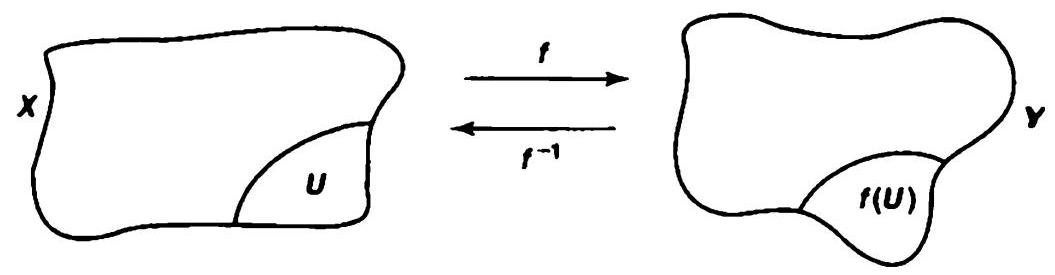
\includegraphics[width=0.9\textwidth]{images/18.1.jpg}
\end{center}
\hspace*{3em} 

Figure 18.1

This remark shows that a homeomorphism \(f : X \rightarrow  Y\) gives us a bijective correspondence not only between \(X\) and \(Y\) but between the collections of open sets of \(X\) and of \(Y\) . As a result, any property of \(X\) that is entirely expressed in terms of the topology of \(X\) (that is, in terms of the open sets of \(X\) ) yields, via the correspondence \(f\) , the corresponding property for the space \(Y\) . Such a property of \(X\) is called a \index{topological property} of \(X\) .

You may have studied in modern algebra the notion of an \index{isomorphism} between algebraic objects such as groups or rings. An isomorphism is a bijective correspondence that preserves the algebraic structure involved. The analogous concept in topology is that of homeomorphism; it is a bijective correspondence that preserves the topological structure involved.

Now suppose that \(f : X \rightarrow  Y\) is an injective continuous map, where \(X\) and \(Y\) are topological spaces. Let \(Z\) be the image set \(f( X)\) , considered as a subspace of \(Y\) ; then the function \({f}^{\prime } : X \rightarrow  Z\) obtained by restricting the range of \(f\) is bijective. If \({f}^{\prime }\) happens to be a homeomorphism of \(X\) with \(Z\) , we say that the map \(f : X \rightarrow  Y\) is a topological \index{imbedding}, or simply an imbedding, of \(X\) in \(Y\) .

\begin{centeredblock}
\begin{example}
	The function \(f : \mathbb{R} \rightarrow  \mathbb{R}\) given by \(f( x)  = {3x} + 1\) is a homeomorphism See Figure 18 2. If we define \(g \cdot  \mathbb{R} \rightarrow  \mathbb{R}\) by the equation

\[
g( y)  = \frac{1}{3}( {y - 1})
\]

then one can check easily that \(f( {g( y) })  = y\) and \(g( {f( x) })  = x\) for all real numbers \(x\) and \(y\) It follows that \(f\) is bijective and that \(g = {f}^{-1}\) , the continuity of \(f\) and \(g\) is a familiar result from calculus.
\end{example}
\end{centeredblock}

\begin{centeredblock}
\begin{example}
	The function \(F : ( {-1,1})  \rightarrow  \mathbb{R}\) defined by

\[
F( x)  = \frac{x}{1 - {x}^{2}}
\]

is a homeomorphism See Figure 18.3 We have already noted in Example 9 of \(§3\) that \(F\) is a bijective order-preserving correspondence, its inverse is the function \(G\) defined by

\[
G( y)  = \frac{2y}{1 + {( 1 + 4{y}^{2}) }^{1/2}}.
\]

The fact that \(F\) is a homeomorphism can be proved in two ways One way is to note that because \(F\) is order preserving and bijective, \(F\) carnes a basis element for the order topology in(-1,1)onto a basis element for the order topology in \(\mathbb{R}\) and vice versa As a result, \(F\) is automatically a homeomorphism of(-1,1)with \(\mathbb{R}\) (both in the order topology) Since the order topology on(-1,1)and the usual (subspace) topology agree, \(F\) is a homeomorphism of(-1,1)with \(\mathbb{R}\)

\begin{center}
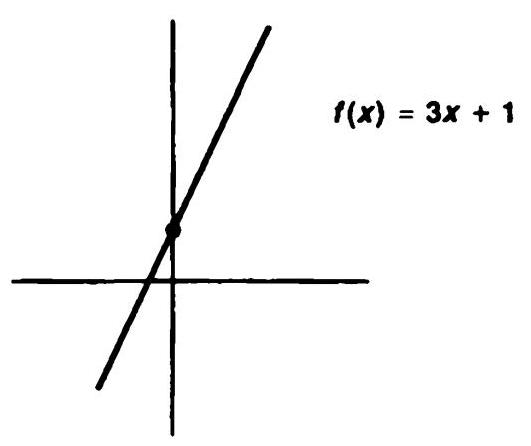
\includegraphics[width=0.4\textwidth]{images/18.2.jpg}
\end{center}
\hspace*{3em}

Figure 18.2

\begin{center}
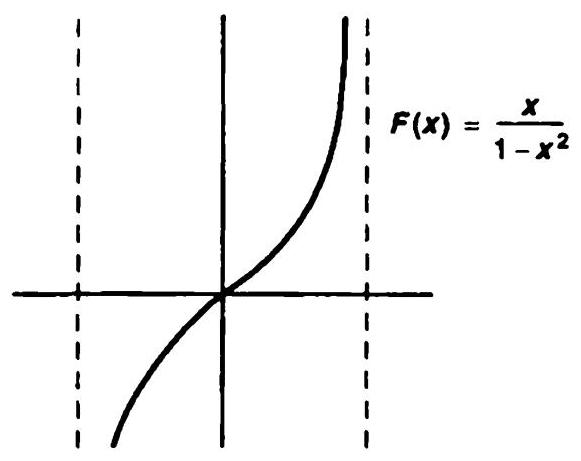
\includegraphics[width=0.5\textwidth]{images/18.3.jpg}
\end{center}
\hspace*{3em}

Figure 18.3

A second way to show \(F\) a homeomorphism is to use the continuity of the algebraic functions and the square-root function to show that both \(F\) and \(G\) are continuous These are familiar facts from calculus
\end{example}
\end{centeredblock}

\begin{centeredblock}
\begin{example}
	A bijective function \(f : X \rightarrow  Y\) can be continuous without being a homeomorphism One such function is the identity map \(g\;{\mathbb{R}}_{\ell } \rightarrow  \mathbb{R}\) considered in Example 3 Another is the following Let \(\index{S@\({S}^{1}\)} \index{S@${S}^{1}$}{S}^{1}\) denote the unit circle.

\[
{S}^{1} = \{  {x \times  y \mid  {x}^{2} + {y}^{2} = 1}\}  ,
\]

considered as a subspace of the plane \({\mathbb{R}}^{2}\) , and let

\[
F \cdot  \lbrack 0,1) \rightarrow  {S}^{1}
\]

be the map defined by \(f( t)  = ( {\cos {2\pi t},\sin {2\pi t}})\) . The fact that \(f\) is bijective and continuous follows from famuliar properties of the trigonometric functions. But the function \({f}^{-1}\) is not continuous The image under \(f\) of the open set \(U = [  {0,\frac{1}{4}})\) of the domain, for instance, is not open in \({S}^{1}\) , for the point \(p = f( 0)\) lies in no open set \(V\) of \({\mathbb{R}}^{2}\) such that \(V \cap  {S}^{1} \subset  f( U)\) . See Figure 18.4.

\begin{center}
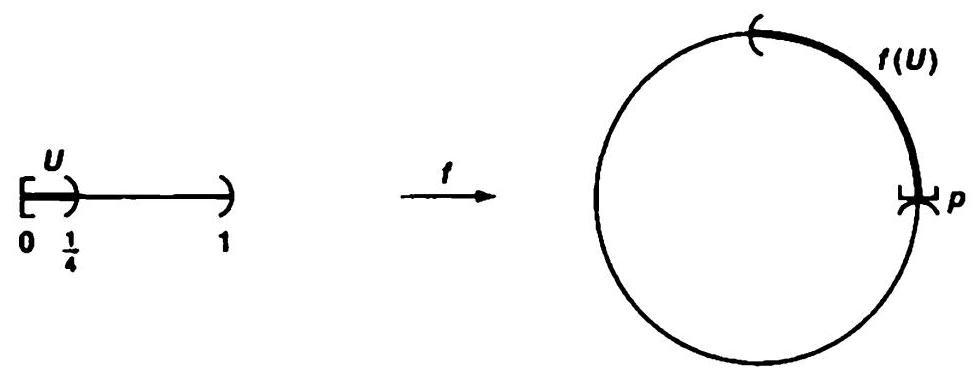
\includegraphics[width=0.9\textwidth]{images/18.4.jpg}
\end{center}
\hspace*{3em} 

Figure 18.4
\end{example}
\end{centeredblock}

\begin{centeredblock}
\begin{example}
	Consider the function

\[
g : \lbrack 0,1) \rightarrow  {\mathbb{R}}^{2}
\]

obtained from the function \(f\) of the preceding example by expanding the range. The map \(g\) is an example of a continuous injective map that is not an \index{Imbedding}imbedding
\end{example}
\end{centeredblock}

\section*{Constructing Continuous Functions}

How does one go about constructing continuous functions from one topological space to another? There are a number of methods used in analysis, of which some generalize to arbitrary topological spaces and others do not. We study first some constructions that do hold for general topological spaces, deferring consideration of the others until later.

\begin{theorem}[Rules for constructing continuous functions]
	Let \(X,Y\) , and \(Z\) be topological spaces.

(a) (Constant function) If \(f : X \rightarrow  Y\) maps all of \(X\) into the single point \({y}_{O}\) of \(Y\) , then \(f\) is continuous.

(b) (Inclusion) If \(A\) is a subspace of \(X\) , the inclusion function \(j : A \rightarrow  X\) is continuous.

(c) (\index{Quotient map!composites}Composites) If \(f : X \rightarrow  Y\) and \(g : Y \rightarrow  Z\) are continuous, then the map \(g \circ  f : X \rightarrow  Z\) is continuous.

(d) (Restricting the domain) If \(f : X \rightarrow  Y\) is continuous, and if \(A\) is a subspace of \(X\) , then the restricted function \(f \mid  A \cdot  A \rightarrow  Y\) is continuous.

(e) (Restricting or expanding the range) Let \(f \cdot  X \rightarrow  Y\) be continuous. If \(Z\) is a subspace of \(Y\) containing the image set \(f( X)\) , then the function \(g : X \rightarrow  Z\) obtained by restricting the range of \(f\) is continuous. If \(Z\) is a space having \(Y\) as a subspace, then the function \(h : X \rightarrow  Z\) obtained by expanding the range of \(f\) is continuous.

(f) (\index{Continuity: of algebraic operations in \(\mathbb{R}\)!local formulation}Local formulation of continuity) The map \(f : X \rightarrow  Y\) is continuous if \(X\) can be written as the union of open sets \({U}_{\alpha }\) such that \(f \mid  {U}_{\alpha }\) is continuous for each \(\alpha\) .

\end{theorem}
\begin{proof}
(a) Let \(f( x)  = {y}_{0}\) for every \(x\) in \(X\) . Let \(V\) be open in \(Y\) . The set \({f}^{-1}( V)\) equals \(X\) or \(\varnothing\) , depending on whether \(V\) contains \({y}_{0}\) or not. In either case, it is open.

(b) If \(U\) is open in \(X\) , then \({j}^{-1}( U)  = U \cap  A\) , which is open in \(A\) by definition of the subspace topology.

(c) If \(U\) is open in \(Z\) , then \({g}^{-1}( U)\) is open in \(Y\) and \({f}^{-1}( {{g}^{-1}( U) })\) is open in \(X\) . But

\[
{f}^{-1}( {{g}^{-1}( U) })  = {( g \circ  f) }^{-1}( U) ,
\]

by elementary set theory.

(d) The function \(f \mid  A\) equals the composite of the inclusion map \(j : A \rightarrow  X\) and the map \(f : X \rightarrow  Y\) , both of which are continuous.

(e) Let \(f : X \rightarrow  Y\) be continuous. If \(f( X)  \subset  Z \subset  Y\) , we show that the function \(g : X \rightarrow  Z\) obtained from \(f\) is continuous. Let \(B\) be open in \(Z\) . Then \(B = Z \cap  U\) for some open set \(U\) of \(Y\) . Because \(Z\) contains the entire image set \(f( X)\) ,

\[
{f}^{-1}( U)  = {g}^{-1}( B) ,
\]

by elementary set theory. Since \({f}^{-1}( U)\) is open, so is \({g}^{-1}( B)\) .

To show \(h : X \rightarrow  Z\) is continuous if \(Z\) has \(Y\) as a subspace, note that \(h\) is the composite of the map \(f : X \rightarrow  Y\) and the inclusion map \(j : Y \rightarrow  Z\) .

(f) By hypothesis, we can write \(X\) as a union of open sets \({U}_{\alpha }\) , such that \(f \mid  {U}_{\alpha }\) is continuous for each \(\alpha\) . Let \(V\) be an open set in \(Y\) . Then

\[
{f}^{-1}( V)  \cap  {U}_{\alpha } = {( f \mid  {U}_{\alpha }) }^{-1}( V) ,
\]

because both expressions represent the set of those points \(x\) lying in \({U}_{\alpha }\) for which \(f( x)  \in  V\) . Since \(f \mid  {U}_{\alpha }\) is continuous, this set is open in \({U}_{\alpha }\) , and hence open in \(X\) But

\[
{f}^{-1}( V)  = \mathop{\bigcup }\limits_{\alpha }( {{f}^{-1}( V)  \cap  {U}_{\alpha }})
\]

so that \({f}^{-1}( V)\) is also open in \(X\) .
\end{proof}

\begin{theorem}[The \index{pasting lemma}]
	Let \(X = A \cup  B\) , where \(A\) and \(B\) are closed in \(X\) . Let \(f : A \rightarrow  Y\) and \(g : B \rightarrow  Y\) be continuous. If \(f( x)  = g( x)\) for every \(x \in  A \cap  B\) , then \(f\) and \(g\) combine to give a continuous function \(h : X \rightarrow  Y\) , defined by setting \(h( x)  = f( x)\) if \(x \in  A\) , and \(h( x)  = g( x)\) if \(x \in  B\) .
\end{theorem}
\begin{proof}
	Let \(C\) be a closed subset of \(Y\) . Now

\[
{h}^{-1}( C)  = {f}^{-1}( C)  \cup  {g}^{-1}( C) ,
\]

by elementary set theory. Since \(f\) is continuous, \({f}^{-1}( C)\) is closed in \(A\) and, therefore, closed in \(X\) . Similarly, \({g}^{-1}( C)\) is closed in \(B\) and therefore closed in \(X\) . Their union \({h}^{-1}( C)\) is thus closed in \(X\) .

This theorem also holds if \(A\) and \(B\) are open sets in \(X\) ; this is just a special case of the ``local formulation of continuity'' rule given in preceding theorem.

\begin{centeredblock}
\begin{example}
	Let us define a function \(h : \mathbb{R} \rightarrow  \mathbb{R}\) by setting

\[
h( x)  = \{  \begin{array}{ll} x & \text{ for }x \leq  0 \\  x/2 & \text{ for }x \geq  0 \end{array}.
\]

Each of the ``pieces'' of this definition is a continuous function, and they agree on the overlapping part of their domains, which is the one-point set \(\{ 0\}\) . Since their domains are closed in \(\mathbb{R}\) , the function \(h\) is continuous. One needs the ``pieces'' of the function to agree on the overlapping part of their domains in order to have a function at all. The equations

\[
k( x)  = \{  \begin{array}{ll} x - 2 & \text{ for }x \leq  0, \\  x + 2 & \text{ for }x \geq  0, \end{array}.
\]

for instance, do not define a function On the other hand, one needs some limitations on the sets \(A\) and \(B\) to guarantee continuity. The equations

\[
l( x)  = \{  \begin{array}{ll} x - 2 & \text{ for }x < 0, \\  x + 2 & \text{ for }x \geq  0, \end{array}.
\]

for instance, do define a function \(l\) mapping \(\mathbb{R}\) into \(\mathbb{R}\) , and both of the pieces are continuous. But \(l\) is not continuous; the inverse image of the open set(1,3), for instance, is the nonopen set \(\lbrack 0,1)\) See Figure 18.5

\begin{center}
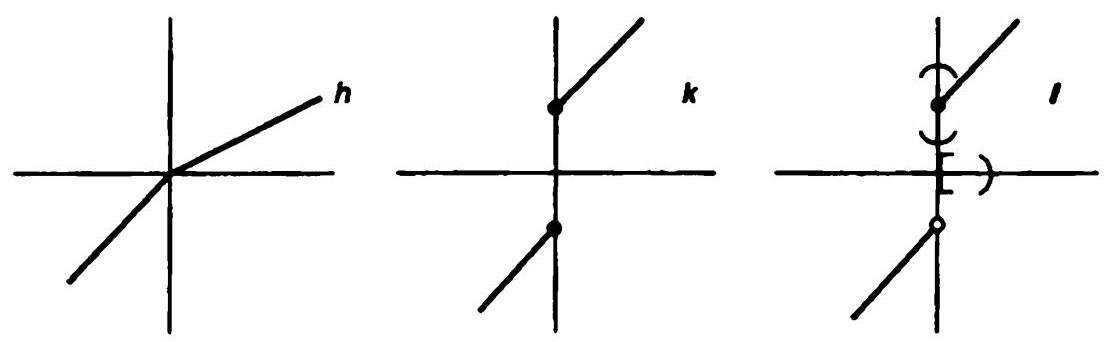
\includegraphics[width=1.0\textwidth]{images/18.5.jpg}
\end{center}
\hspace*{3em}

Figure 18.5
\end{example}
\end{centeredblock}

\end{proof}
\begin{theorem}[Maps into products]
	Let \(f : A \rightarrow  X \times  Y\) be given by the equation

\[
f( a)  = ( {{f}_{1}( a) ,{f}_{2}( a) }) .
\]

Then \(f\) is continuous if and only if the functions

\[
{f}_{1} : A \rightarrow  X\;\text{ and }\;{f}_{2} : A \rightarrow  Y
\]

are continuous.

The maps \({f}_{1}\) and \({f}_{2}\) are called the \index{coordinate function} of \(f\) .

\end{theorem}
\begin{proof}
Let \({\pi }_{1}.X \times  Y \rightarrow  X\) and \({\pi }_{2} : X \times  Y \rightarrow  Y\) be projections onto the first and second factors, respectively. These maps are continuous. For \({\pi }_{1}^{-1}( U)  = U \times  Y\) and \({\pi }_{2}^{-1}( V)  = X \times  V\) , and these sets are open if \(U\) and \(V\) are open. Note that for each \(a \in  A\) ,

\[
{f}_{1}( a)  = {\pi }_{1}( {f( a) }) \;\text{ and }\;{f}_{2}( a)  = {\pi }_{2}( {f( a) }) .
\]

If the function \(f\) is continuous, then \({f}_{1}\) and \({f}_{2}\) are composites \index{Composite: of functions!of continuous functions}of continuous functions and therefore continuous. Conversely, suppose that \({f}_{1}\) and \({f}_{2}\) are continuous. We show that for each basis element \(U \times  V\) for the topology of \(X \times  Y\) , its inverse image \({f}^{-1}( {U \times  V})\) is open. A point \(a\) is in \({f}^{-1}( {U \times  V})\) if and only if \(f( a)  \in  U \times  V\) , that is, if and only if \({f}_{1}( a)  \in  U\) and \({f}_{2}( a)  \in  V\) . Therefore,

\[
{f}^{-1}( {U \times  V})  = {f}_{1}^{-1}( U)  \cap  {f}_{2}^{-1}( V) .
\]

Since both of the sets \({f}_{1}^{-1}( U)\) and \({f}_{2}^{-1}( V)\) are open, so is their intersection.

There is no useful criterion for the continuity of a map \(f : A \times  B \rightarrow  X\) whose domain is a \index{Product space}product space. One might conjecture that \(f\) is continuous if it is continuous ``in each variable separately,'' but this conjecture is not true. (See Exercise 12.)
\end{proof}

\begin{centeredblock}
\begin{example}
	In calculus, a parametrized curve in the plane is defined to be a continuous map \(f[  {a,b}]   \rightarrow  {\mathbb{R}}^{2}\) It is often expressed in the form \(f( t)  = ( {x( t) ,y( t) })\) ; and one frequently uses the fact that \(f\) is a continuous function of \(t\) if both \(x\) and \(y\) are Similarly, a vector field in the plane

\[
\mathbf{v}( {x,y})  = P( {x,y}) \mathbf{i} + Q( {x,y}) \mathbf{j}
\]

\[
= ( {P( {x,y}) ,Q( {x,y}) })
\]

is said to be continuous if both \(P\) and \(Q\) are continuous functions, or equivalently, if \(\mathbf{v}\) is continuous as a map of \({\mathbb{R}}^{2}\) into \({\mathbb{R}}^{2}\) . Both of these statements are simply special cases of the preceding theorem.
\end{example}
\end{centeredblock}

One way of forming continuous functions that is used a great deal in analysis is to take sums, differences, products, or \index{Quotient space (see also Quotient topology)} quotients of continuous real-valued functions. It is a standard theorem that if \(f.g.X \rightarrow  \mathbb{R}\) are continuous, then \(f + g,f - g\) , and \(f \cdot  g\) are continuous, and \(f/g\) is continuous if \(g( x)  \neq  0\) for all \(x\) . We shall consider this theorem in \(§{21}\) .

Yet another method for constructing continuous functions that is familiar from analysis is to take the limit of an infinite sequence of functions. There is a theorem to the effect that if a sequence of continuous real-valued functions of a real variable converges \index{Uniform metric (see also Uniform topology)} uniformly to a limit function, then the limit function is necessarily continuous. This theorem is called the \index{Uniform Limit Theorem}. It is used, for instance, to demonstrate the continuity of the trigonometric functions, when one defines these functions rigorously using the infinite series definitions of the sine and cosine. This theorem generalizes to a theorem about maps of an arbitrary topological space \(X\) into a metric space \(Y\) . We shall prove it in \(§{21}\) .

\section*{Exercises}
\begin{enumerate}[itemsep=0.4em, parsep=0pt, topsep=0pt, partopsep=0pt, leftmargin=*, label=\arabic*., ref=\arabic*]
\item Prove that for functions \(f : \mathbb{R} \rightarrow  \mathbb{R}\) , the \(\epsilon  - \delta\) definition of continuity implies the open set definition.
\item Suppose that \(f : X \rightarrow  Y\) is continuous. If \(x\) is a limit point of the subset \(A\) of \(X\) , is it necessarily true that \(f( x)\) is a limit point of \(f( A)\) ?
\item Let \(X\) and \({X}^{\prime }\) denote a single set in the two topologies \(\mathcal{T}\) and \({\mathcal{T}}^{\prime }\) , respectively. Let \(i : {X}^{\prime } \rightarrow  X\) be the identity function.
  \begin{enumerate}[itemsep=0.2em, parsep=0pt, topsep=0pt, partopsep=0pt, leftmargin=*, label=(\alph*), align=left]
  \item Show that \(i\) is continuous \(\Leftrightarrow  {\mathcal{T}}^{\prime }\) is finer than \(\mathcal{T}\) .
  \item Show that \(i\) is a homeomorphism \(\Leftrightarrow  {\mathcal{T}}^{\prime } = \mathcal{T}\) .
  \end{enumerate}
\item Given \({x}_{0} \in  X\) and \({y}_{0} \in  Y\) , show that the maps \(f : X \rightarrow  X \times  Y\) and \(g : Y \rightarrow\)  \(X \times  Y\) defined by \[ f( x)  = x \times  {y}_{0}\;\text{ and }\;g( y)  = {x}_{0} \times  y \] are imbeddings.
\item Show that the subspace(a, b)of \(\mathbb{R}\) is homeomorphic with(0,1)and the subspace \([  {a,b}]\) of \(\mathbb{R}\) is homeomorphic with \([  {0,1}]\)
\item Find a function \(f : \mathbb{R} \rightarrow  \mathbb{R}\) that is continuous at precisely one point.
\item
  \begin{enumerate}[itemsep=0.2em, parsep=0pt, topsep=0pt, partopsep=0pt, leftmargin=*, label=(\alph*), align=left]
  \item Suppose that \(f : \mathbb{R} \rightarrow  \mathbb{R}\) is ``continuous from the right,'' that is, \[ \mathop{\lim }\limits_{{x \rightarrow  {a}^{ + }}}f( x)  = f( a) \] for each \(a \in  \mathbb{R}\) . Show that \(f\) is continuous when considered as a function from \({\mathbb{R}}_{\ell }\) to \(\mathbb{R}\) .

  \item Can you conjecture what functions \(f \cdot  \mathbb{R} \rightarrow  \mathbb{R}\) are continuous when considered as maps from \(\mathbb{R}\) to \({\mathbb{R}}_{\ell }\) ? As maps from \({\mathbb{R}}_{\ell }\) to \({\mathbb{R}}_{\ell }\) ? We shall return to this question in Chapter 3.
  \end{enumerate}
\item Let \(Y\) be an ordered set in the order topology. Let \(f,g : X \rightarrow  Y\) be continuous. (a) Show that the set \(\{ x \mid  f( x)  \leq  g( x) \}\) is closed in \(X\)
  \begin{enumerate}[itemsep=0.2em, parsep=0pt, topsep=0pt, partopsep=0pt, leftmargin=*, label=(\alph*), align=left]
  \item Let \(h : X \rightarrow  Y\) be the function \[ h( x)  = \min \{ f( x) ,g( x) \} . \] Show that \(h\) is continuous [Hint: Use the \index{Pasting lemma}pasting lemma.]
  \end{enumerate}
\item Let \(\{  {A}_{\alpha }\}\) be a collection of subsets of \(X\) ; let \(X = \mathop{\bigcup }\limits_{\alpha }{A}_{\alpha }\) . Let \(f : X \rightarrow  Y\) ; suppose that \(f \mid  {A}_{\alpha }\) , is continuous for each \(\alpha\) .
  \begin{enumerate}[itemsep=0.2em, parsep=0pt, topsep=0pt, partopsep=0pt, leftmargin=*, label=(\alph*), align=left]
  \item Show that if the collection \(\{  {A}_{\alpha }\}\) is finite and each set \({A}_{\alpha }\) is closed, then \(f\) is continuous.
  \item Find an example where the collection \(\{  {A}_{\alpha }\}\) is countable and each \({A}_{\alpha }\) is closed, but \(f\) is not continuous.
  \item An indexed family of sets \(\{  {A}_{\alpha }\}\) is said to be \index{Locally finite family} locally finite if each point \(x\) of \(X\) has a neighborhood that intersects \({A}_{\alpha }\) for only finitely many values of \(\alpha\) . Show that if the family \(\{  {A}_{\alpha }\}\) is locally finite and each \({A}_{\alpha }\) is closed, then \(f\) is continuous.
  \end{enumerate}
\item Let \(f \cdot  A \rightarrow  B\) and \(g : C \rightarrow  D\) be continuous functions. Let us define a map \(f \times  g : A \times  C \rightarrow  B \times  D\) by the equation \[ ( {f \times  g}) ( {a \times  c})  = f( a)  \times  g( c) . \] Show that \(f \times  g\) is continuous.
\item Let \(F : X \times  Y \rightarrow  Z\) . We say that \(F\) is continuous in each variable separately if for each \({y}_{0}\) in \(Y\) , the map \(h : X \rightarrow  Z\) defined by \(h( x)  = F( {x \times  {y}_{0}})\) is continuous, and for each \({x}_{0}\) in \(X\) , the map \(k \cdot  Y \rightarrow  Z\) defined by \(k( y)  = F( {{x}_{0} \times  y})\) is continuous. Show that if \(F\) is continuous, then \(F\) is continuous in each variable separately.
\item Let \(F : \mathbb{R} \times  \mathbb{R} \rightarrow  \mathbb{R}\) be defined by the equation \[ F( {x \times  y})  = \{  \begin{array}{ll} {xy}/( {{x}^{2} + {y}^{2}}) & \text{ if }x \times  y \neq  0 \times  0. \\  0 & \text{ if }x \times  y = 0 \times  0 \end{array}. \]
  \begin{enumerate}[itemsep=0.2em, parsep=0pt, topsep=0pt, partopsep=0pt, leftmargin=*, label=(\alph*), align=left]
  \item Show that \(F\) is continuous in each variable separately.
  \item Compute the function \(g : \mathbb{R} \rightarrow  \mathbb{R}\) defined by \(g( x)  = F( {x \times  x})\) .
  \item Show that \(F\) is not continuous
  \end{enumerate}
\item Let \(A \subset  X\) ; let \(f : A \rightarrow  Y\) be continuous; let \(Y\) be Hausdorff. Show that if \(f\) may be extended to a continuous function \(g.\bar{A} \rightarrow  Y\) , then \(g\) is uniquely determined by \(f\)
\end{enumerate}
\section*{§ 19 The Product Topology}

We now return, for the remainder of the chapter, to the consideration of various methods for imposing topologies on sets

Previously, we defined a topology on the product \(X \times  Y\) of two topological spaces. In the present section, we generalize this definition to more general cartesian products.

So let us consider the cartesian products

\[
{X}_{1} \times  \cdots  \times  {X}_{n}\;\text{ and }\;{X}_{1} \times  {X}_{2} \times  \cdots ,
\]

where each \({X}_{i}\) is a topological space There are two possible ways to proceed. One way is to take as basis all sets of the form \({U}_{1} \times  \cdots  \times  {U}_{n}\) in the first case, and of the form \({U}_{1} \times  {U}_{2} \times  \cdots\) in the second case, where \({U}_{i}\) is an open set of \({X}_{i}\) for each \(i\) . This procedure does indeed define a topology on the cartesian product; we shall call it the \index{box topology}.

Another way to proceed is to generalize the subbasis formulation of the definition, given in \(§{15}\) . In this case, we take as a subbasis all sets of the form \({\pi }_{i}^{-1}( {U}_{i})\) , where \(i\) is any index and \({U}_{i}\) is an open set of \({X}_{i}\) . We shall call this topology the product topology.

How do these topologies differ? Consider the typical basis element \(B\) for the second topology. It is a finite intersection of subbasis elements \({\pi }_{i}^{-1}( {U}_{i})\) , say for \(i =\)  \({i}_{1},\ldots ,{i}_{k}\) . Then a point \(\mathbf{x}\) belongs to \(B\) if and only if \({\pi }_{i}( \mathbf{x})\) belongs to \({U}_{i}\) for \(i =\)  \({i}_{1},\ldots ,{i}_{k}\) ; there is no restriction on \({\pi }_{i}( x)\) for other values of \(i\) .

It follows that these two topologies agree for the finite cartesian product and differ for the infinite product. What is not clear is why we seem to prefer the second topology. This is the question we shall explore in this section

Before proceeding, however, we shall introduce a more general notion of cartesian product. So far, we have defined the cartesian product of an indexed family of sets only in the cases where the index set was the set \(\{ 1,\ldots ,n\}\) or the set \({\mathbb{Z}}_{ + }\) Now we consider the case where the index set is completely arbitrary.

\begin{definition}
	Let \(J\) be an index set. Given a set \(X\) , we define a \(J\) -tuple of elements of \(X\) to be a function \(\mathbf{x} : J \rightarrow  X\) . If \(\alpha\) is an element of \(J\) , we often denote the value of \(x\) at \(\alpha\) by \({x}_{\alpha }\) rather than \(x( \alpha )\) ; we call it the \(\alpha\) th coordinate of \(x\) . And we often denote the function \(x\) itself by the symbol

\[
{( {x}_{\alpha }) }_{\alpha  \in  J},
\]

which is as close as we can come to a ``tuple notation'' for an arbitrary index set \(J\) . We denote the set of all \(J\) -tuples of elements of \(X\) by \(\index{X@\({X}^{J}\)} \index{X@${X}^{J}$}{X}^{J}\) .
\end{definition}

\begin{definition}
	Let \({\{  {A}_{\alpha }\}  }_{\alpha  \in  J}\) be an indexed family of sets; let \(X = \mathop{\bigcup }\limits_{{\alpha  \in  J}}{A}_{\alpha }\) . The cartesian product of this indexed family, denoted by

\[
\mathop{\prod }\limits_{{\alpha  \in  J}}{A}_{\alpha }
\]

is defined to be the set of all \(J\) -tuples \({( {x}_{\alpha }) }_{\alpha  \in  J}\) of elements of \(X\) such that \({x}_{\alpha } \in  {A}_{\alpha }\) for each \(\alpha  \in  J\) That is, it is the set of all functions

\[
\mathbf{x} : J \rightarrow  \mathop{\bigcup }\limits_{{\alpha  \in  J}}{A}_{\alpha }
\]

such that \(\mathbf{x}( \alpha )  \in  {A}_{\alpha }\) for each \(\alpha  \in  J\) .

Occasionally we denote the product simply by \(\prod {A}_{\alpha }\) , and its general element by \(( {x}_{\alpha })\) , if the index set is understood
\end{definition}

If all the sets \({A}_{\alpha }\) are equal to one set \(X\) , then the cartesian product \(\mathop{\prod }\limits_{{\alpha  \in  J}}{A}_{\alpha }\) is just the set \({X}^{J}\) of all \(J\) -tuples of elements of \(X\) . We sometimes use ``tuple notation'' for the elements of \({X}^{J}\) , and sometimes we use functional notation, depending on which is more convenient.

\begin{definition}
	Let \({\{  {X}_{\alpha }\}  }_{\alpha  \in  J}\) be an indexed family of topological spaces. Let us take as a basis for a topology on the product space

\[
\mathop{\prod }\limits_{{\alpha  \in  J}}{X}_{\alpha }
\]

the collection of all sets of the form

\[
\mathop{\prod }\limits_{{\alpha  \in  J}}{U}_{\alpha }
\]

where \({U}_{\alpha }\) is open in \({X}_{\alpha }\) , for each \(\alpha  \in  J\) . The topology generated by this basis is called the \index{Box topology}box topology
\end{definition}

This collection satisfies the first condition for a basis because \(\prod {X}_{\alpha }\) is itself a basis element; and it satisfies the second condition because the intersection of any two basis elements is another basis element.

\[
( {\mathop{\prod }\limits_{{\alpha  \in  J}}{U}_{\alpha }})  \cap  ( {\mathop{\prod }\limits_{{\alpha  \in  J}}{V}_{\alpha }})  = \mathop{\prod }\limits_{{\alpha  \in  J}}( {{U}_{\alpha } \cap  {V}_{\alpha }}) .
\]

Now we generalize the subbasis formulation of the definition. Let

\[
{\pi }_{\beta } : \mathop{\prod }\limits_{{\alpha  \in  J}}{X}_{\alpha } \rightarrow  {X}_{\beta }
\]

be the function assigning to each element of the product space its \(\beta\) th coordinate,

\[
{\pi }_{\beta }( {( {x}_{\alpha }) }_{\alpha  \in  J})  = {x}_{\beta };
\]

it is called the \index{projection map}ing associated with the index \(\beta\) .

\begin{definition}
	Let \({S}_{\beta }\) denote the collection

\[
{S}_{\beta } = \{  {{\pi }_{\beta }^{-1}( {U}_{\beta })  \mid  {U}_{\beta }\text{ open in }{X}_{\beta }}\}  ,
\]

and let \(S\) denote the union of these collections,

\[
S = \mathop{\bigcup }\limits_{{\beta  \in  J}}{S}_{\beta }
\]

The topology generated by the subbasis \(S\) is called the product topology. In this topology \(\mathop{\prod }\limits_{{\alpha  \in  J}}{X}_{\alpha }\) is called a product space.
\end{definition}

To compare these topologies, we consider the basis \(\mathcal{B}\) that \(\mathcal{S}\) generates. The collection \(\mathcal{B}\) consists of all finite intersections of elements of \(\mathcal{S}\) . If we intersect elements belongingg to the same one of the sets \({S}_{\beta }\) , we do not get anything new, because

\[
{\pi }_{\beta }^{-1}( {U}_{\beta })  \cap  {\pi }_{\beta }^{-1}( {V}_{\beta })  = {\pi }_{\beta }^{-1}( {{U}_{\beta } \cap  {V}_{\beta }})
\]

the intersection of two elements of \({S}_{\beta }\) , or of finitely many such elements, is again an element of \({S}_{\beta }\) . We get something new only when we intersect elements from different sets \({S}_{\beta }\) . The typical element of the basis \(\mathcal{B}\) can thus be described as follows \(\ldots ,{\beta }_{n}\) be a finite set of distinct indices from the index set \(J\) , and let \({U}_{{\beta }_{i}}\) be an open set in \({X}_{{\beta }_{i}}\) for \(i = 1,\ldots ,n\) . Then

\[
B = {\pi }_{{\beta }_{1}}^{-1}( {U}_{{\beta }_{1}})  \cap  {\pi }_{{\beta }_{2}}^{-1}( {U}_{{\beta }_{2}})  \cap   \cdot   \cap  {\pi }_{{\beta }_{n}}^{-1}( {U}_{{\beta }_{n}})
\]

is the typical element of \(\mathcal{B}\) .

Now a point \(\mathbf{x} = ( {x}_{\alpha })\) is in \(B\) if and only if its \({\beta }_{1}\) th coordinate is in \({U}_{{\beta }_{1}}\) , its \({\beta }_{2}\) th coordinate is in \({U}_{{\beta }_{2}}\) , and so on. There is no restriction whatever on the \(\alpha\) th coordinate of \(\mathbf{x}\) if \(\alpha\) is not one of the indices \({\beta }_{1},\ldots ,{\beta }_{n}\) . As a result, we can write \(B\) as the product

\[
B = \mathop{\prod }\limits_{{\alpha  \in  J}}{U}_{\alpha }
\]

where \({U}_{\alpha }\) denotes the entire space \({X}_{\alpha }\) if \(\alpha  \neq  {\beta }_{1},\ldots ,{\beta }_{n}\) .

All this is summarized in the following theorem:

\begin{theorem}[Comparison of the box and product topologies]
	The box topology on \(\prod {X}_{\alpha }\) has as basis all sets of the form \(\prod {U}_{\alpha }\) , where \({U}_{\alpha }\) is open in \({X}_{\alpha }\) for each \(\alpha\) . The product topology on \(\prod {X}_{\alpha }\) has as basis all sets of the form \(\prod {U}_{\alpha }\) , where \({U}_{\alpha }\) is open in \({X}_{\alpha }\) for each \(\alpha\) and \({U}_{\alpha }\) equals \({X}_{\alpha }\) except for finitely many values of \(\alpha\) .

Two things are immediately clear First, for finite products \(\mathop{\prod }\limits_{{\alpha  = 1}}^{n}{X}_{\alpha }\) the two topologies are precisely the same. Second, the box topology is in general finer than the product topology.

What is not so clear is why we prefer the product topology to the box topology. The answer will appear as we continue our study of topology. We shall find that a number of important theorems about finite products will also hold for arbitrary products if we use the product topology, but not if we use the box topology. As a result, the product topology is extremely important in mathematics. The box topology is not so important; we shall use it primarily for constructing counterexamples. Therefore, we make the following convention:

Whenever we consider the product \(\prod {X}_{\alpha }\) , we shall assume it is given the product topology unless we specifically state otherwise.

Some of the theorems we proved for the product \(X \times  Y\) hold for the product \(\prod {X}_{\alpha }\) no matter which topology we use. We list them here; most of the proofs are left to the exercises.

\end{theorem}
\begin{theorem}
	Suppose the topology on each space \({X}_{\alpha }\) is given by a basis \({\mathcal{B}}_{\alpha }\) . The collection of all sets of the form

\[
\mathop{\prod }\limits_{{\alpha  \in  J}}{B}_{\alpha }
\]

where \({B}_{\alpha } \in  {\mathcal{B}}_{\alpha }\) for each \(\alpha\) , will serve as a basis for the box topology on \(\mathop{\prod }\limits_{{\alpha  \in  J}}{X}_{\alpha }\) .

The collection of all sets of the same form, where \({B}_{\alpha } \in  {\mathcal{B}}_{\alpha }\) for finitely many indices \(\alpha\) and \({B}_{\alpha } = {X}_{\alpha }\) for all the remaining indices, will serve as a basis for the \(\begin{matrix} \text{ product topology }\mathop{\prod }\limits_{{\alpha  \in  J}}{X}_{\alpha }. \end{matrix}\)

\begin{centeredblock}
\begin{example}
	Consider euclidean \(n\) -space \({\mathbb{R}}^{n}\) . A basis for \(\mathbb{R}\) consists of all open intervals in \(\mathbb{R}\) ; hence a basis for the topology of \({\mathbb{R}}^{n}\) consists of all products of the form

\[
( {{a}_{1},{b}_{1}})  \times  ( {{a}_{2},{b}_{2}})  \times   \cdot  \; \times  ( {{a}_{n},{b}_{n}}) .
\]

Since \({\mathbb{R}}^{n}\) is a finite product, the box and product topologies agree Whenever we consider \({\mathbb{R}}^{n}\) , we will assume that it is given this topology, unless we specifically state otherwise
\end{example}
\end{centeredblock}

\end{theorem}
\begin{theorem}
	Let \({A}_{\alpha }\) be a subspace of \({X}_{\alpha }\) , for each \(\alpha  \in  J\) . Then \(\prod {A}_{\alpha }\) is a subspace of \(\prod {X}_{\alpha }\) if both products are given the box topology, or if both products are given the product topology.

\end{theorem}
\begin{theorem}
	If each space \({X}_{\alpha }\) is a Hausdorff space, then \(\prod {X}_{\alpha }\) is a Hausdorff space in both the box and product topologies.

\end{theorem}
\begin{theorem}
	Let \(\{  {X}_{\alpha }\}\) be an indexed family of spaces; let \({A}_{\alpha } \subset  {X}_{\alpha }\) for each \(\alpha\) . If \(\prod {X}_{\alpha }\) is given either the product or the box topology, then

\[
\prod {\widetilde{A}}_{\alpha } = \bar{\prod }\overline{{A}_{\alpha }}.
\]

\end{theorem}
\begin{proof}
Let \(\mathbf{x} = ( {x}_{\alpha })\) be a point of \(\prod {\bar{A}}_{\alpha }\) ; we show that \(\mathbf{x} \in  \overline{\prod {A}_{\alpha }}\) . Let \(U = \prod {U}_{\alpha }\) be a basis element for either the box or product topology that contains \(\mathbf{x}\) . Since \({x}_{\alpha } \in  {\widetilde{A}}_{\alpha }\) , we can choose a point \({y}_{\alpha } \in  {U}_{\alpha } \cap  {A}_{\alpha }\) for each \(\alpha\) . Then \(\mathbf{y} = ( {y}_{\alpha })\) belongs to both \(U\) and \(\prod {A}_{\alpha }\) . Since \(U\) is arbitrary, it follows that \(x\) belongs to the closure of \(\prod {A}_{\alpha }\) .

Conversely, suppose \(\mathbf{x} = ( {x}_{\alpha })\) lies in the closure of \(\prod {A}_{\alpha }\) , in either topology. We show that for any given index \(\beta\) , we have \({x}_{\beta } \in  {A}_{\beta }\) . Let \({V}_{\beta }\) be an arbitrary open set of \({X}_{\beta }\) containing \({x}_{\beta }\) . Since \({\pi }_{\beta }^{-1}( {V}_{\beta })\) is open in \(\prod {X}_{\alpha }\) in either topology, it contains a point \(\mathbf{y} = ( {y}_{\alpha })\) of \(\prod {A}_{\alpha }\) . Then \({y}_{\beta }\) belongs to \({V}_{\beta } \cap  {A}_{\beta }\) . It follows that \({x}_{\beta } \in  {\widetilde{A}}_{\beta }\) .

So far, no reason has appeared for preferring the product to the box topology. It is when we try to generalize our previous theorem about continuity of maps into product spaces that a difference first arises. Here is a theorem that does not hold if \(\prod {X}_{\alpha }\) is given the box topology:
\end{proof}

\begin{theorem}
	Let \(f : A \rightarrow  \mathop{\prod }\limits_{{\alpha  \in  J}}{X}_{\alpha }\) be given by the equation

\[
f( a)  = {( {f}_{\alpha }( a) ) }_{\alpha  \in  J},
\]

where \({f}_{\alpha } : A \rightarrow  {X}_{\alpha }\) for each \(\alpha\) . Let \(\prod {X}_{\alpha }\) have the product topology. Then the function \(f\) is continuous if and only if each function \({f}_{\alpha }\) is continuous.

\end{theorem}
\begin{proof}
Let \({\pi }_{\beta }\) be the projection of the product onto its \(\beta\) th factor. The function \({\pi }_{\beta }\) is continuous, for if \({U}_{\beta }\) is open in \({X}_{\beta }\) , the set \({\pi }_{\beta }^{-1}( {U}_{\beta })\) is a subbasis element for the product topology on \({X}_{\alpha }\) . Now suppose that \(f : A \rightarrow  \prod {X}_{\alpha }\) is continuous. The function \({f}_{\beta }\) equals the composite \({\pi }_{\beta } \circ  f\) ; being the composite of two continuous functions, it is continuous.

Conversely, suppose that each \index{Coordinate function}coordinate function \({f}_{\alpha }\) is continuous. To prove that \(f\) is continuous, it suffices to prove that the inverse image under \(f\) of each subbasis element is open in \(A\) , we remarked on this fact when we defined continuous functions. A typical subbasis element for the product topology on \(\prod {X}_{\alpha }\) is a set of the form \({\pi }_{\beta }^{-1}( {U}_{\beta })\) , where \(\beta\) is some index and \({U}_{\beta }\) is open in \({X}_{\beta }\) . Now

\[
{f}^{-1}( {{\pi }_{\beta }^{-1}( {U}_{\beta }) })  = {f}_{\beta }^{-1}( {U}_{\beta }) ,
\]

because \({f}_{\beta } = {\pi }_{\beta } \circ  f\) . Since \({f}_{\beta }\) is continuous, this set is open in \(A\) , as desired.

Why does this theorem fail if we use the box topology? Probably the most convincing thing to do is to look at an example.
\end{proof}

\begin{centeredblock}
\begin{example}
	Consider \({\mathbb{R}}^{\omega }\) , the countably infinite product of \(\mathbb{R}\) with itself. Recall that

\[
{\mathbb{R}}^{\omega } = \mathop{\prod }\limits_{{n \in  {\mathbb{Z}}_{ + }}}{X}_{n}
\]

where \({X}_{n} = \mathbb{R}\) for each \(n\) Let us define a function \(f\mathbb{R} \rightarrow  {\mathbb{R}}^{\omega }\) by the equation

\[
f( t)  = ( {t,t,t,\ldots }) ,
\]

the \(n\) th coordinate function of \(f\) is the function \({f}_{n}( t)  = t\) Each of the coordinate functions \({f}_{n}.\mathbb{R} \rightarrow  \mathbb{R}\) is continuous; therefore, the function \(f\) is continuous if \({\mathbb{R}}^{\omega }\) is given the product topology. But \(f\) is not continuous if \({\mathbb{R}}^{\omega }\) is given the box topology Consider, for example, the basis element

\[
B = ( {-1,1})  \times  ( {-\frac{1}{2},\frac{1}{2}})  \times  ( {-\frac{1}{3},\frac{1}{3}})  \times  \cdots
\]

for the box topology. We assert that \({f}^{-1}( B)\) is not open in \(\mathbb{R}\) . If \({f}^{-1}( B)\) were open in \(\mathbb{R}\) , it would contain some interval \(( {-\delta ,\delta })\) about the point 0 . This would mean that \(f( ( {-\delta ,\delta }) )  \subset  B\) , so that, applying \({\pi }_{n}\) to both sides of the inclusion,

\[
{f}_{n}( ( {-\delta ,\delta }) )  = ( {-\delta ,\delta })  \subset  ( {-1/n,1/n})
\]

for all \(n\) , a contradiction
\end{example}
\end{centeredblock}

\section*{Exercises}
\begin{enumerate}[itemsep=0.4em, parsep=0pt, topsep=0pt, partopsep=0pt, leftmargin=*, label=\arabic*., ref=\arabic*]
\item Prove Theorem 19.2
\item Prove Theorem 19.3.
\item Prove Theorem 19.4
\item Show that \(( {{X}_{1} \times  \cdots  \times  {X}_{n - 1}})  \times  {X}_{n}\) is homeomorphic with \({X}_{1} \times  \cdots  \times  {X}_{n}\) .
\item One of the implications stated in Theorem 19.6 holds for the box topology. Which one?
\item Let \({\mathbf{x}}_{1},{\mathbf{x}}_{2},\ldots\) be a sequence of the points of the product space \(\prod {X}_{\alpha }\) . Show that this sequence converges to the point \(\mathbf{x}\) if and only if the sequence \({\pi }_{\alpha }( {\mathbf{x}}_{1}) ,{\pi }_{\alpha }( {\mathbf{x}}_{2})\) , \begin{itemize} \item converges to \({\pi }_{\alpha }( \mathbf{x})\) for each \(\alpha\) . Is this fact true if one uses the box topology instead of the product topology? \end{itemize}
\item Let \(\index{R@\({\mathbb{R}}^{\infty }\)} \index{R@${\mathbb{R}}^{\infty }$}{\mathbb{R}}^{\infty }\) be the subset of \({\mathbb{R}}^{\omega }\) consisting of all sequences that are ``eventually zero,'' that is, all sequences \(( {{x}_{1},{x}_{2},\ldots })\) such that \({x}_{i} \neq  0\) for only finitely many values of \(i\) . What is the closure of \({\mathbb{R}}^{\infty }\) in \({\mathbb{R}}^{\omega }\) in the box and product topologies? Justify your answer.
\item Given sequences \(( {{a}_{1},{a}_{2},\ldots })\) and \(( {{b}_{1},{b}_{2},\ldots })\) of real numbers with \({a}_{i} > 0\) for all \(i\) , define \(h : {\mathbb{R}}^{\omega } \rightarrow  {\mathbb{R}}^{\omega }\) by the equation \[ h( ( {{x}_{1},{x}_{2},\ldots }) )  = ( {{a}_{1}{x}_{1} + {b}_{1},{a}_{2}{x}_{2} + {b}_{2},\ldots }) . \] Show that if \({\mathbb{R}}^{\omega }\) is given the product topology, \(h\) is a homeomorphism of \({\mathbb{R}}^{\omega }\) with itself. What happens if \({\mathbb{R}}^{\omega }\) is given the box topology?
\item Show that the choice axiom is equivalent to the statement that for any indexed family \({\{  {A}_{\alpha }\}  }_{\alpha  \in  J}\) of nonempty sets, with \(J \neq  0\) , the cartesian product \[ \mathop{\prod }\limits_{{\alpha  \in  J}}{A}_{\alpha } \] is not empty.
\item Let \(A\) be a set; let \({\{  {X}_{\alpha }\}  }_{\alpha  \in  J}\) be an indexed family of spaces; and let \({\{  {f}_{\alpha }\}  }_{\alpha  \in  J}\) be an indexed family of functions \({f}_{\alpha } : A \rightarrow  {X}_{\alpha }\) .
  \begin{enumerate}[itemsep=0.2em, parsep=0pt, topsep=0pt, partopsep=0pt, leftmargin=*, label=(\alph*), align=left]
  \item Show there is a unique coarsest topology \(\mathcal{T}\) on \(A\) relative to which each of the functions \({f}_{\alpha }\) is continuous.
  \item Let \[ {S}_{\beta } = \{  {{f}_{\beta }^{-1}( {U}_{\beta })  \mid  {U}_{\beta }\text{ is open in }{X}_{\beta }}\}  , \] and let \(S =  \cup  {S}_{\beta }\) . Show that \(S\) is a subbasis for \(\mathcal{T}\)
  \item Show that a map \(g : Y \rightarrow  A\) is continuous relative to \(\mathcal{T}\) if and only if each map \({f}_{\alpha } \circ  g\) is continuous.
  \item Let \(f : A \rightarrow  \prod {X}_{\alpha }\) be defined by the equation \[ f( a)  = {( {f}_{\alpha }( a) ) }_{\alpha  \in  J}; \] let \(Z\) denote the subspace \(f( A)\) of the product space \(\prod {X}_{\alpha }\) . Show that the image under \(f\) of each element of \(\mathcal{T}\) is an open set of \(Z\) .
  \end{enumerate}
\end{enumerate}
\section*{§ 20 The Metric Topology}

One of the most important and frequently used ways of imposing a topology on a set is to define the topology in terms of a metric on the set. Topologies given in this way lie at the heart of modern analysis, for example. In this section, we shall define the \index{metric topology} and shall give a number of examples. In the next section, we shall consider some of the properties that metric topologies satisfy.

\begin{definition}
	A metric on a set \(X\) is a function

\[
d : X \times  X \rightarrow  R
\]

having the following properties:

(1) \(d( {x,y})  \geq  0\) for all \(x,y \in  X\) ; equality holds if and only if \(x = y\) .

(2) \(d( {x,y})  = d( {y,x})\) for all \(x,y \in  X\) .

(3) (\index{Triangle inequality}) \(d( {x,y})  + d( {y,z})  \geq  d( {x,z})\) , for all \(x,y,z \in  X\) .

Given a metric \(d\) on \(X\) , the number \(d( {x,y})\) is often called the \index{distance} between \(x\) and \(y\) in the metric \(d\) Given \(\epsilon  > 0\) , consider the set

\[
{B}_{d}( {x,\epsilon })  = \{ y \mid  d( {x,y})  < \epsilon \}
\]

of all points \(y\) whose \index{Distance}distance from \(x\) is less than \(\epsilon\) . It is called the \(\epsilon\) -ball centered at \(x\) . Sometimes we omit the metric \(d\) from the notation and write this ball simply as \(\index{B@\(B( {x,\epsilon })\)} \index{B@$B( {x,\epsilon })$}B( {x,\epsilon })\) , when no confusion will arise.
\end{definition}

\begin{definition}
	If \(d\) is a metric on the set \(X\) , then the collection of all \(\epsilon\) -balls \({B}_{d}( {x,\epsilon })\) , for \(x \in  X\) and \(\epsilon  > 0\) , is a basis for a topology on \(X\) , called the \index{Metric topology}metric topology induced by \(d\) .
\end{definition}

The first condition for a basis is trivial, since \(x \in  B( {x,\epsilon })\) for any \(\epsilon  > 0\) . Before checking the second condition for a basis, we show that if \(y\) is a point of the basis element \(B( {x,\epsilon })\) , then there is a basis element \(B( {y,\delta })\) centered at \(y\) that is contained in \(B( {x,\epsilon })\) . Define \(\delta\) to be the positive number \(\epsilon  - d( {x,y})\) . Then \(B( {y,\delta })  \subset  B( {x,\epsilon })\) , for if \(z \in  B( {y,\delta })\) , then \(d( {y,z})  < \epsilon  - d( {x,y})\) , from which we conclude that

\[
d( {x,z})  \leq  d( {x,y})  + d( {y,z})  < \epsilon .
\]

See Figure 20.1.

Now to check the second condition for a basis, let \({B}_{1}\) and \({B}_{2}\) be two basis elements and let \(y \in  {B}_{1} \cap  {B}_{2}\) . We have just shown that we can choose positive numbers \({\delta }_{1}\) and \({\delta }_{2}\) so that \(B( {y,{\delta }_{1}})  \subset  {B}_{1}\) and \(B( {y,{\delta }_{2}})  \subset  {B}_{2}\) . Letting \(\delta\) be the smaller of \({\delta }_{1}\) and \({\delta }_{2}\) , we conclude that \(B( {y,\delta })  \subset  {B}_{1} \cap  {B}_{2}\) .

Using what we have just proved, we can rephrase the definition of the metric topology as follows:

\begin{center}
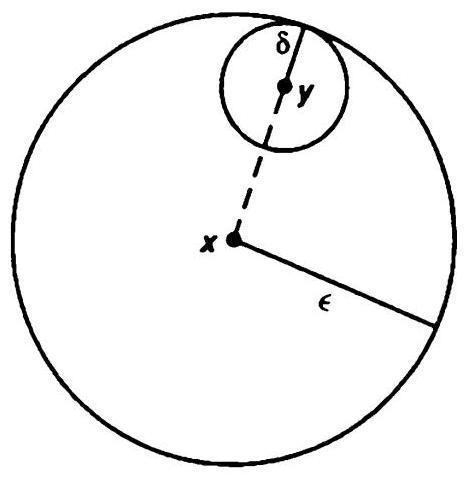
\includegraphics[width=0.4\textwidth]{images/20.1.jpg}
\end{center}
\hspace*{3em} 

Figure 20.1

A set \(U\) is open in the metric topology induced by \(d\) if and only if for each \(y \in  U\) , there is a \(\delta  > 0\) such that \({B}_{d}( {y,\delta })  \subset  U\) .

Clearly this condition implies that \(U\) is open. Conversely, if \(U\) is open, it contains a basis element \(B = {B}_{d}( {x,\epsilon })\) containing \(y\) , and \(B\) in turn contains a basis element \({B}_{d}( {y,\delta })\) centered at \(y\)

\begin{centeredblock}
\begin{example}
	Given a set \(X\) , define

\[
d( {x,y})  = 1\;\text{ if }x \neq  y,
\]

\[
d( {x,y})  = 0\;\text{ if }x = y
\]

It is trivial to check that \(d\) is a metric. The topology it induces is the discrete topology; the basis element \(B( {x,1})\) , for example, consists of the point \(x\) alone.
\end{example}
\end{centeredblock}

\begin{centeredblock}
\begin{example}
	The standard metric on the real numbers \(\mathbb{R}\) is defined by the equation

\[
d( {x,y})  = | {x - y}|
\]

It is easy to check that \(d\) is a metric. The topology it induces is the same as the order topology: Each basis element(a, b)for the order topology is a basis element for the metric topology, indeed,

\[
( {a,b})  = B( {x,\epsilon }) ,
\]

where \(x = ( {a + b}) /2\) and \(\epsilon  = ( {b - a}) /2\) . And conversely, each \(\epsilon\) -ball \(B( {x,\epsilon })\) equals an open interval the interval \(( {x - \epsilon ,x + \epsilon })\) .
\end{example}
\end{centeredblock}

\begin{definition}
	If \(X\) is a topological space, \(X\) is said to be metrizable if there exists a metric \(d\) on the set \(X\) that induces the topology of \(X\) . A metric space is a \index{metrizable space} \(X\) together with a specific metric \(d\) that gives the topology of \(X\) .
\end{definition}

Many of the spaces important for mathematics are metrizable, but some are not. Metrizability is always a highly desirable attribute for a space to possess, for the existence of a metric gives one a valuable tool for proving theorems about the space.

It is, therefore, a problem of fundamental importance in topology to find conditions on a topological space that will guarantee it is metrizable. One of our goals in Chapter 4 will be to find such conditions; they are expressed there in the famous theorem called Urysohn's metrization theorem. Further metrization theorems appear in Chapter 6. In the present section we shall content ourselves with proving merely that \({\mathbb{R}}^{n}\) and \({\mathbb{R}}^{\omega }\) are metrizable.

Although the \index{Product topology!metrizability}metrizability problem is an important problem in topology, the study \index{First-countability!of metric space}of metric spaces as such does not properly belong to topology as much as it does to analysis Metrzability of a space depends only on the topology of the space in question, but properties that involve a specific \index{Discrete topology!metric for}metric for \(X\) in general do not. For instance, one can make the following definition in a metric space.

\begin{definition}
	Let \(X\) be a metric space with metric \(d\) . A subset \(A\) of \(X\) is said to be \index{Bounded set} bounded if there is some number \(M\) such that

\[
d( {{a}_{1},{a}_{2}})  \leq  M
\]

for every pair \({a}_{1},{a}_{2}\) of points of \(A\) . If \(A\) is \index{Metric!bounded}bounded and nonempty, the \index{Diameter of a set} diameter of \(A\) is defined to be the number

\[
\operatorname{diam}A = \sup \{  {d( {{a}_{1},{a}_{2}})  \mid  {a}_{1},{a}_{2} \in  A}\}  .
\]
\end{definition}

Boundedness of a set is not a topological property, for it depends on the particular metric \(d\) that is used for \(X\) . For instance, if \(X\) is a metric space with metric \(d\) , then there exists a metric \(\bar{d}\) that gives the topology of \(X\) , relative to which every subset of \(X\) is bounded. It is defined as follows

\begin{theorem}
	Let \(X\) be a metric space with metric \(d\) . Define \(\index{d@\(\widetilde{d}\)} : X \times  X \rightarrow  \mathbb{R}\) by the equation

\[
\bar{d}( {x,y})  = \min \{ d( {x,y}) ,1\}
\]

Then \(\bar{d}\) is a metric that induces the same topology as \(d\) .

The metric \(\bar{d}\) is called the standard \index{bounded metric} corresponding to \(d\) .

\end{theorem}
\begin{proof}
Checking the first two conditions for a metric is trivial. Let us check the triangle inequality:

\[
\bar{d}( {x,z})  \leq  \bar{d}( {x,y})  + \bar{d}( {y,z}) .
\]

Now if either \(d( {x,y})  \geq  1\) or \(d( {y,z})  \geq  1\) , then the right side of this inequality is at least 1, since the left side is (by definition) at most 1, the inequality holds. It remains to consider the case in which \(d( {x,y})  < 1\) and \(d( {y,z})  < 1\) . In this case, we have

\[
d( {x,z})  \leq  d( {x,y})  + d( {y,z})  = \bar{d}( {x,y})  + \bar{d}( {y,z}) .
\]

Since \(\bar{d}( {x,z})  \leq  d( {x,z})\) by definition, the \index{Triangle inequality}triangle inequality holds for \(\bar{d}\) .

Now we note that in any metric space, the collection of \(\epsilon\) -balls with \(\epsilon  < 1\) forms a basis for the metric topology, for every basis element containing \(x\) contains such an \(\epsilon\) -ball centered at \(x\) . It follows that \(d\) and \(\bar{d}\) induce the same topology on \(X\) , because the collections of \(\epsilon\) -balls with \(\epsilon  < 1\) under these two metrics are the same collection.

Now we consider some familiar spaces and show they are metrizable.
\end{proof}

\begin{definition}
	Given \(\mathbf{x} = ( {{x}_{1},\ldots ,{x}_{n}})\) in \({\mathbb{R}}^{n}\) , we define the \index{norm} of \(\mathbf{x}\) by the equation

\[
\parallel x\parallel  = {( {x}_{1}^{2} + \cdots  + {x}_{n}^{2}) }^{1/2}
\]

and we define the \index{euclidean metric} \(d\) on \({\mathbb{R}}^{n}\) by the equation

\[
d( {\mathbf{x},\mathbf{y}})  = \parallel \mathbf{x} - \mathbf{y}\parallel  = {[  {( {x}_{1} - {y}_{1}) }^{2} + \cdots  + {( {x}_{n} - {y}_{n}) }^{2}]  }^{1/2}.
\]
\end{definition}

We define the square metric \(\index{rho@\(\rho\)}\) by the equation

\[
\rho ( {\mathbf{x},\mathbf{y}})  = \max \{  {| {{x}_{1} - {y}_{1}}| ,\ldots ,| {{x}_{n} - {y}_{n}}| }\}  .
\]

The proof that \(d\) is a metric requires some work; it is probably already familiar to you. If not, a proof is outlined in the exercises. We shall seldom have occasion to use this metric on \({\mathbb{R}}^{n}\)

To show that \(\rho\) is a metric is easier. Only the triangle inequality is nontrivial. From the triangle inequality for \(\mathbb{R}\) it follows that for each positive integer \(i\) ,

\[
| {{x}_{i} - {z}_{i}}|  \leq  | {{x}_{i} - {y}_{i}}|  + | {{y}_{i} - {z}_{i}}| .
\]

Then by definition of \(\rho\) ,

\[
| {{x}_{t} - {z}_{i}}|  \leq  \rho ( {\mathbf{x},\mathbf{y}})  + \rho ( {\mathbf{y},\mathbf{z}}) .
\]

As a result

\[
\rho ( {\mathbf{x},\mathbf{z}})  = \max \{  | {{x}_{i} - {z}_{i}}| \}   \leq  \rho ( {\mathbf{x},\mathbf{y}})  + \rho ( {\mathbf{y},\mathbf{z}}) ,
\]

as desired.

On the real line \(\mathbb{R} = {\mathbb{R}}^{1}\) , these two metrics coincide with the standard metric for \(\mathbb{R}\) . In the plane \({\mathbb{R}}^{2}\) , the basis elements under \(d\) can be pictured as circular regions, while the basis elements under \(\rho\) can be pictured as square regions.

We now show that each of these metrics induces the usual topology on \({\mathbb{R}}^{n}\) . We need the following lemma:

\begin{lemma}
	Let \(d\) and \({d}^{\prime }\) be two metrics on the set \(X\) ; let \(\mathcal{T}\) and \({\mathcal{T}}^{\prime }\) be the topologies they induce, respectively. Then \({\mathcal{T}}^{\prime }\) is finer than \(\mathcal{T}\) if and only if for each \(x\) in \(X\) and each \(\epsilon  > 0\) , there exists a \(\delta  > 0\) such that

\[
{B}_{{d}^{\prime }}( {x,\delta })  \subset  {B}_{d}( {x,\epsilon })
\]
\end{lemma}

\begin{proof}
Suppose that \({\mathcal{T}}^{\prime }\) is finer than \(\mathcal{T}\) Given the basis element \({B}_{d}( {x,\epsilon })\) for \(\mathcal{T}\) , there is by Lemma 13.3 a basis element \({B}^{\prime }\) for the topology \({\mathcal{T}}^{\prime }\) such that \(x \in  {B}^{\prime } \subset  {B}_{d}( {x,\epsilon })\) . Within \({B}^{\prime }\) we can find a ball \({B}_{{d}^{\prime }}( {x,\delta })\) centered at \(x\) .

Conversely, suppose the \(\delta\) - \(\epsilon\) condition holds Given a basis element \(B\) for \(\mathcal{T}\) containing \(x\) , we can find within \(B\) a ball \({B}_{d}( {x,\epsilon })\) centered at \(x\) . By the given condition, there is a \(\delta\) such that \({B}_{{d}^{\prime }}( {x,\delta })  \subset  {B}_{d}( {x,\epsilon })\) . Then Lemma 13.3 applies to show \({\mathcal{T}}^{\prime }\) is finer than \(\mathcal{T}\) .
\end{proof}

\begin{theorem}
	The topologies on \({\mathbb{R}}^{n}\) induced by the \index{Euclidean metric}euclidean metric \(d\) and the square metric \(\rho\) are the same as the product topology on \({\mathbb{R}}^{n}\) .

\end{theorem}
\begin{proof}
Let \(\mathbf{x} = ( {{x}_{1},\ldots ,{x}_{n}})\) and \(\mathbf{y} = ( {{y}_{1},\ldots ,{y}_{n}})\) be two points of \({\mathbb{R}}^{n}\) . It is simple algebra to check that

\[
\rho ( {\mathbf{x},\mathbf{y}})  \leq  d( {\mathbf{x},\mathbf{y}})  \leq  \sqrt{n}\rho ( {\mathbf{x},\mathbf{y}})
\]

The first inequality shows that

\[
{B}_{d}( {\mathbf{x},\epsilon })  \subset  {B}_{\rho }( {\mathbf{x},\epsilon })
\]

for all \(\mathbf{x}\) and \(\epsilon\) , since if \(d( {\mathbf{x},\mathbf{y}})  < \epsilon\) , then \(\rho ( {\mathbf{x},\mathbf{y}})  < \epsilon\) also. Similarly, the second inequality shows that

\[
{B}_{\rho }( {\mathbf{x},\epsilon /\sqrt{n}})  \subset  {B}_{d}( {\mathbf{x},\epsilon })
\]

for all \(x\) and \(\epsilon\) . It follows from the preceding lemma that the two metric topologies are the same.

Now we show that the product topology is the same as that given by the metric \(\rho\) . First, let

\[
B = ( {{a}_{1},{b}_{1}})  \times   \cdot   \times  ( {{a}_{n},{b}_{n}})
\]

be a basis element for the product topology, and let \(\mathbf{x} = ( {{x}_{1},\ldots ,{x}_{n}})\) be an element of \(B\) . For each \(i\) , there is an \({\epsilon }_{i}\) such that

\[
( {{x}_{l} - {\epsilon }_{i},{x}_{i} + {\epsilon }_{l}})  \subset  ( {{a}_{i},{b}_{i}}) ,
\]

choose \(\epsilon  = \min \{  {{\epsilon }_{1},\ldots ,{\epsilon }_{n}}\}\) . Then \({B}_{\rho }( {\mathbf{x},\epsilon })  \subset  B\) , as you can readily check. As a result, the \(\rho\) -topology is finer than the product topology.

Conversely, let \({B}_{\rho }( {\mathbf{x},\epsilon })\) be a basis element for the \(\rho\) -topology. Given the element \(\mathbf{y} \in  {B}_{\rho }( {\mathbf{x},\epsilon })\) , we need to find a basis element \(B\) for the product topology such that

\[
\mathbf{y} \in  B \subset  {B}_{\rho }( {\mathbf{x},\epsilon }) \text{ . }
\]

But this is trivial, for

\[
{B}_{\rho }( {\mathbf{x},\epsilon })  = ( {{x}_{1} - \epsilon ,{x}_{1} + \epsilon })  \times  \cdots  \times  ( {{x}_{n} - \epsilon ,{x}_{n} + \epsilon })
\]

is itself a basis element for the product topology.

Now we consider the infinite cartesian product \({\mathbb{R}}^{\omega }\) . It is natural to try to generalize the metrics \(d\) and \(\rho\) to this space. For instance, one can attempt to define a metric \(d\) on \({\mathbb{R}}^{\omega }\) by the equation

\[
d( {\mathbf{x},\mathbf{y}})  = {[  \mathop{\sum }\limits_{{i = 1}}^{\infty }{( {x}_{i} - {y}_{i}) }^{2}]  }^{1/2}.
\]

But this equation does not always make sense, for the series in question need not converge. (This equation does define a metric on a certain important subset of \({\mathbb{R}}^{\omega }\) , however; see the exercises.)

Similarly, one can attempt to generalize the square metric \(\rho\) to \({\mathbb{R}}^{\omega }\) by defining

\[
\rho ( {\mathbf{x},\mathbf{y}})  = \sup \{  | {{x}_{n} - {y}_{n}}| \}  .
\]

Again, this formula does not always make sense. If however we replace the usual metric \(d( {x,y})  = | {x - y}|\) on \(\mathbb{R}\) by its bounded counterpart \(d( {x,y})  = \min \{ | {x - y}| ,1\}\) , then this definition does make sense; it gives a metric on \({\mathbb{R}}^{\omega }\) called the uniform metric.

The uniform metric can be defined more generally on the cartesian product \({\mathbb{R}}^{J}\) for arbitrary \(J\) , as follows:
\end{proof}

\begin{definition}
	Given an index set \(J\) , and given points \(\mathbf{x} = {( {x}_{\alpha }) }_{\alpha  \in  J}\) and \(\mathbf{y} = {( {y}_{\alpha }) }_{\alpha  \in  J}\) of \({\mathbb{R}}^{J}\) , let us define a metric \(\bar{\rho }\) on \({\mathbb{R}}^{J}\) by the equation

\[
\bar{\rho }( {\mathbf{x},\mathbf{y}})  = \sup \{ \bar{d}( {{x}_{\alpha },{y}_{\alpha }})  \mid  \alpha  \in  J\} ,
\]

where \(\bar{d}\) is the \index{Standard bounded metric}standard bounded metric on \(\mathbb{R}\) . It is easy to check that \(\bar{\rho }\) is indeed a metric; it is called the uniform metric on \({\mathbb{R}}^{J}\) , and the topology it induces is called the uniform topology.
\end{definition}

The relation between this topology and the product and box topologies is the following:

\begin{theorem}
	The uniform topology on \({\mathbb{R}}^{J}\) is finer than the product topology and coarser than the box topology; these three topologies are all different if \(J\) is infinite.

\end{theorem}
\begin{proof}
Suppose that we are given a point \(\mathbf{x} = {( {x}_{\alpha }) }_{\alpha  \in  J}\) and a product topology basis element \(\prod {U}_{\alpha }\) about \(\mathbf{x}\) . Let \({\alpha }_{1},\ldots ,{\alpha }_{n}\) be the indices for which \({U}_{\alpha } \neq  \mathbb{R}\) . Then for each \(i\) , choose \({\epsilon }_{i} > 0\) so that the \({\epsilon }_{i}\) -ball centered at \({x}_{{\alpha }_{i}}\) in the \(d\) metric is contained in \({U}_{{\alpha }_{i}}\) ; this we can do because \({U}_{{\alpha }_{i}}\) is open in \(\mathbb{R}\) . Let \(\epsilon  = \min \{  {{\epsilon }_{1},\ldots ,{\epsilon }_{n}}\}\) ; then the \(\epsilon\) -ball centered at \(\mathbf{x}\) in the \(\bar{\rho }\) metric is contained in \(\prod {U}_{\alpha }\) . For if \(\mathbf{z}\) is a point of \({\mathbb{R}}^{J}\) such that \(\widetilde{\rho }( {\mathbf{x},\mathbf{z}})  < \epsilon\) , then \(\widetilde{d}( {{x}_{\alpha },{z}_{\alpha }})  < \epsilon\) for all \(\alpha\) , so that \(\mathbf{z} \in  \prod {U}_{\alpha }\) . It follows that the uniform topology is finer than the product topology.

On the other hand, let \(B\) be the \(\epsilon\) -ball centered at \(\mathbf{x}\) in the \(\bar{\rho }\) metric. Then the box neighborhood

\[
U = \prod ( {{x}_{\alpha } - \frac{1}{2}\epsilon ,{x}_{\alpha } + \frac{1}{2}\epsilon })
\]

of \(\mathbf{x}\) is contained in \(B\) . For if \(\mathbf{y} \in  U\) , then \(\bar{d}( {{x}_{\alpha },{y}_{\alpha }})  < \frac{1}{2}\epsilon\) for all \(\alpha\) , so that \(\bar{\rho }( {\mathbf{x},\mathbf{y}})  \leq\)  \(\frac{1}{2}\epsilon\) .

Showing these three topologies are different if \(J\) is infinite is a task we leave to the exercises.

In the case where \(J\) is infinite, we still have not determined whether \({\mathbb{R}}^{J}\) is metrizable in either the box or the product topology. It turns out that the only one of these cases where \({\mathbb{R}}^{J}\) is metrizable is the case where \(J\) is countable and \({\mathbb{R}}^{J}\) has the product topology. As we shall see.
\end{proof}

\begin{theorem}
	Let \(\bar{d}( {a,b})  = \min \{ | {a - b}| ,1\}\) be the standard bounded metric on \(\mathbb{R}\) . If \(\mathbf{x}\) and \(\mathbf{y}\) are two points of \({\mathbb{R}}^{\omega }\) , define

\[
D( {\mathbf{x},\mathbf{y}})  = \sup \{  \frac{\bar{d}( {{x}_{i},{y}_{i}}) }{i}\}  .
\]

Then \(D\) is a metric that induces the product topology on \({\mathbb{R}}^{\omega }\) .

\end{theorem}
\begin{proof}
The properties of a metric are satisfied trivially except for the triangle inequality, which is proved by noting that for all \(i\) ,

\[
\frac{\bar{d}( {{x}_{i},{z}_{l}}) }{i} \leq  \frac{\bar{d}( {{x}_{l},{y}_{i}}) }{i} + \frac{\bar{d}( {{y}_{l},{z}_{i}}) }{i} \leq  D( {\mathbf{x},\mathbf{y}})  + D( {\mathbf{y},\mathbf{z}}) ,
\]

so that

\[
\sup \{  \frac{\bar{d}( {{x}_{i},{z}_{i}}) }{i}\}   \leq  D( {\mathbf{x},\mathbf{y}})  + D( {\mathbf{y},\mathbf{z}}) .
\]

The fact that \(D\) gives the product topology requires a \index{Little ell-two topology} little more work. First, let \(U\) be open in the metric topology and let \(\mathbf{x} \in  U\) ; we'find an open set \(V\) in the product topology such that \(\mathbf{x} \in  V \subset  U\) . Choose an \(\epsilon\) -ball \({B}_{D}( {\mathbf{x},\epsilon })\) lying in \(U\) . Then choose \(N\) large enough that \(1/N < \epsilon\) . Finally, let \(V\) be the basis element for the product topology

\[
V = ( {{x}_{1} - \epsilon ,{x}_{1} + \epsilon })  \times  \cdots  \times  ( {{x}_{N} - \epsilon ,{x}_{N} + \epsilon })  \times  \mathbb{R} \times  \mathbb{R} \times  \cdots .
\]

We assert that \(V \subset  {B}_{D}( {\mathbf{x},\epsilon })\) : Given any \(\mathbf{y}\) in \({\mathbb{R}}^{\omega }\) ,

\[
\frac{\bar{d}( {{x}_{i},{y}_{i}}) }{i} \leq  \frac{1}{N}\;\text{ for }i \geq  N.
\]

Therefore,

\[
D( {\mathbf{x},\mathbf{y}})  \leq  \max \{  {\frac{\bar{d}( {{x}_{1},{y}_{1}}) }{1},\cdots ,\frac{\bar{d}( {{x}_{N},{y}_{N}}) }{N},\frac{1}{N}}\}  .
\]

If \(\mathbf{y}\) is in \(V\) , this expression is less than \(\epsilon\) , so that \(V \subset  {B}_{D}( {\mathbf{x},\epsilon })\) , as desired.

Conversely, consider a basis element

\[
U = \mathop{\prod }\limits_{{i \in  {\mathbb{Z}}_{ + }}}{U}_{i}
\]

for the product topology, where \({U}_{i}\) is open in \(\mathbb{R}\) for \(i = {\alpha }_{1},\ldots ,{\alpha }_{n}\) and \({U}_{i} = \mathbb{R}\) for all other indices i. Given \(\mathbf{x} \in  U\) , we find an open set \(V\) of the metric topology such that \(\mathbf{x} \in  V \subset  U\) . Choose an interval \(( {{x}_{t} - {\epsilon }_{i},{x}_{i} + {\epsilon }_{i}})\) in \(\mathbb{R}\) centered about \({x}_{t}\) and lying in \({U}_{i}\) for \(i = {\alpha }_{1},\ldots ,{\alpha }_{n}\) ; choose each \({\epsilon }_{i} \leq  1\) . Then define

\[
\epsilon  = \min \{  {{\epsilon }_{i}/\mathrm{i} \mid  \mathrm{i} = {\alpha }_{1},\ldots ,{\alpha }_{n}}\}  .
\]

We assert that

\[
\mathbf{x} \in  {B}_{D}( {\mathbf{x},\epsilon })  \subset  U\text{ . }
\]

Let \(\mathbf{y}\) be a point of \({B}_{D}( {\mathbf{x},\epsilon })\) . Then for all \(i\) ,

\[
\frac{\bar{d}( {{x}_{i},{y}_{i}}) }{\mathrm{i}} \leq  D( {\mathbf{x},\mathbf{y}})  < \epsilon .
\]

Now if \(i = {\alpha }_{1},\ldots ,{\alpha }_{n}\) , then \(\epsilon  \leq  {\epsilon }_{i}/i\) , so that \(\widetilde{d}( {{x}_{i},{y}_{i}})  < {\epsilon }_{i} \leq  1\) ; it follows that \(| {{x}_{i} - {y}_{i}}|  < {\epsilon }_{i}\) . Therefore, \(\mathbf{y} \in  \prod {U}_{i}\) , as desired.
\end{proof}

\section*{Exercises}
\begin{enumerate}[itemsep=0.4em, parsep=0pt, topsep=0pt, partopsep=0pt, leftmargin=*, label=\arabic*., ref=\arabic*]
\item
  \begin{enumerate}[itemsep=0.2em, parsep=0pt, topsep=0pt, partopsep=0pt, leftmargin=*, label=(\alph*), align=left]
  \item In \({\mathbb{R}}^{n}\) , define \[ {d}^{\prime }( {\mathbf{x},\mathbf{y}})  = | {{x}_{1} - {y}_{1}}|  + \cdots  + | {{x}_{n} - {y}_{n}}| . \] Show that \({d}^{\prime }\) is a metric that induces the usual topology of \({\mathbb{R}}^{n}\) . Sketch the basis elements under \({d}^{\prime }\) when \(n = 2\) .

  \item More generally, given \(p \geq  1\) , define \[ {d}^{\prime }( {\mathbf{x},\mathbf{y}})  = {[  \mathop{\sum }\limits_{{i = 1}}^{n}{| {x}_{i} - {y}_{i}| }^{p}]  }^{1/p} \] for \(\mathbf{x},\mathbf{y} \in  {\mathbb{R}}^{n}\) . Assume that \({d}^{\prime }\) is a metric. Show that it induces the usual topology on \({\mathbb{R}}^{n}\) .
  \end{enumerate}
\item Show that \(\mathbb{R} \times  \mathbb{R}\) in the dictionary order topology is metrizable.
\item Let \(X\) be a metric space with metric \(d\) .
  \begin{enumerate}[itemsep=0.2em, parsep=0pt, topsep=0pt, partopsep=0pt, leftmargin=*, label=(\alph*), align=left]
  \item Show that \(d : X \times  X \rightarrow  \mathbb{R}\) is continuous.
  \item Let \({X}^{\prime }\) denote a space having the same underlying set as \(X\) . Show that if \(d : {X}^{\prime } \times  {X}^{\prime } \rightarrow  \mathbb{R}\) is continuous, then the topology of \({X}^{\prime }\) is finer than the topology of \(X\) . One can summarize the result of this exercise as follows: If \(X\) has a metric \(d\) , then the topology induced by \(d\) is the coarsest topology relative to which the function \(d\) is continuous. 4. Consider the product, uniform, and box topologies on \({\mathbb{R}}^{\omega }\) .
  \item In which topologies are the following functions from \(\mathbb{R}\) to \({\mathbb{R}}^{\omega }\) continuous? \[ f( t)  = ( {t,{2t},{3t},\ldots }) , \] \[ g( t)  = ( {t,t,t,\ldots }) , \] \[ h( t)  = ( {t,\frac{1}{2}t,\frac{1}{3}t,\ldots }) . \]
  \item In which topologies do the following sequences converge? \[ {\mathbf{w}}_{1} = ( {1,1,1,1,\ldots }) ,\;{\mathbf{x}}_{1} = ( {1,1,1,1,\ldots }) , \] \[ {\mathbf{w}}_{2} = ( {0,2,2,2,\ldots }) ,\;{\mathbf{x}}_{2} = ( {0,\frac{1}{2},\frac{1}{2},\frac{1}{2},\ldots }) , \] \[ {\mathbf{w}}_{3} = ( {0,0,3,3,\ldots }) ,\;{\mathbf{x}}_{3} = ( {0,0,\frac{1}{3},\frac{1}{3}\ldots }) , \] ... ... \[ {\mathbf{y}}_{1} = ( {1,0,0,0,\ldots }) ,\;{\mathbf{z}}_{1} = ( {1,1,0,0,\ldots }) , \] \[ {\mathbf{y}}_{2} = ( {\frac{1}{2},\frac{1}{2},0,0,\ldots }) ,\;{\mathbf{z}}_{2} = ( {\frac{1}{2},\frac{1}{2},0,0,\ldots }) , \] \[ {\mathbf{y}}_{3} = ( {\frac{1}{3},\frac{1}{3},\frac{1}{3},0,\ldots }) ,\;{\mathbf{z}}_{3} = ( {\frac{1}{3},\frac{1}{3},0,0,\ldots }) , \] ... ...
  \end{enumerate}
\item Let \({\mathbb{R}}^{\infty }\) be the subset of \({\mathbb{R}}^{\omega }\) consisting of all sequences that are eventually zero. What is the closure of \({\mathbb{R}}^{\infty }\) in \({\mathbb{R}}^{\omega }\) in the uniform topology? Justify your answer.
\item Let \(\bar{\rho }\) be the uniform metric on \({\mathbb{R}}^{\omega }\) . Given \(\mathbf{x} = ( {{x}_{1},{x}_{2},\ldots })  \in  {\mathbb{R}}^{\omega }\) and given \(0 < \epsilon  < 1\) , let \[ U( {\mathbf{x},\epsilon })  = ( {{x}_{1} - \epsilon ,{x}_{1} + \epsilon })  \times  \cdots  \times  ( {{x}_{n} - \epsilon ,{x}_{n} + \epsilon })  \times  \cdots . \]
  \begin{enumerate}[itemsep=0.2em, parsep=0pt, topsep=0pt, partopsep=0pt, leftmargin=*, label=(\alph*), align=left]
  \item Show that \(U( {\mathbf{x},\epsilon })\) is not equal to the \(\epsilon\) -ball \({B}_{\bar{\rho }}( {\mathbf{x},\epsilon })\) .
  \item Show that \(U( {\mathbf{x},\epsilon })\) is not even open in the uniform topology.
  \item Show that \[ {B}_{\bar{\rho }}( {\mathbf{x},\epsilon })  = \mathop{\bigcup }\limits_{{\delta  < \epsilon }}U( {\mathbf{x},\delta }) . \]
  \end{enumerate}
\item Consider the map \(h : {\mathbb{R}}^{\omega } \rightarrow  {\mathbb{R}}^{\omega }\) defined in Exercise 8 of \(§{19}\) , give \({\mathbb{R}}^{\omega }\) the uniform topology. Under what conditions on the numbers \({a}_{i}\) and \({b}_{i}\) is \(h\) continuous? a homeomorphism?
\item Let \(X\) be the subset of \({\mathbb{R}}^{\omega }\) consisting of all sequences \(\mathbf{x}\) such that \(\sum {x}_{i}^{2}\) converges. Then the formula \[ d( {\mathbf{x},\mathbf{y}})  = {[  \mathop{\sum }\limits_{{i = 1}}^{\infty }{( {x}_{i} - {y}_{i}) }^{2}]  }^{1/2} \] defines a metric on \(X\) . (See Exercise 10.) On \(X\) we have the three topologies it inherits from the box, uniform, and product topologies on \({\mathbb{R}}^{\omega }\) . We have also the topology given by the metric \(d\) , which we call the \({\ell }^{2}\) -topology. (Read ``little ell two.'')
  \begin{enumerate}[itemsep=0.2em, parsep=0pt, topsep=0pt, partopsep=0pt, leftmargin=*, label=(\alph*), align=left]
  \item Show that on \(X\) , we have the inclusions \[ \text{ box topology } \supset  {\ell }^{2}\text{ -topology } \supset  \text{ uniform topology. } \]
  \item The set \({\mathbb{R}}^{\infty }\) of all sequences that are eventually zero is contained in \(X\) . Show that the four topologies that \({\mathbb{R}}^{\infty }\) inherits as a subspace of \(X\) are all distinct.
  \item The set \[ H = \mathop{\prod }\limits_{{n \in  {\mathbb{Z}}_{ + }}}[  {0,1/n}] \] is contained in \(X\) , it is called the \index{Hilbert cube}. Compare the four topologies that \(H\) inherits as a subspace of \(X\) .
  \end{enumerate}
\item Show that the euclidean metric \(d\) on \({\mathbb{R}}^{n}\) is a metric, as follows: If \(\mathbf{x},\mathbf{y} \in  {\mathbb{R}}^{n}\) and \(c \in  \mathbb{R}\) , define \[ \mathbf{x} + \mathbf{y} = ( {{x}_{1} + {y}_{1},\ldots ,{x}_{n} + {y}_{n}}) , \] \[ c\mathbf{x} = ( {c{x}_{1},\ldots ,c{x}_{n}}) , \] \[ \mathbf{x} \cdot  \mathbf{y} = {x}_{1}{y}_{1} + \cdots  + {x}_{n}{y}_{n} \]
  \begin{enumerate}[itemsep=0.2em, parsep=0pt, topsep=0pt, partopsep=0pt, leftmargin=*, label=(\alph*), align=left]
  \item Show that \(\mathbf{x} \cdot  ( {\mathbf{y} + \mathbf{z}})  = ( \begin{array}{ll} \mathbf{x} & \mathbf{y} \end{array})  + ( {\mathbf{x} \cdot  \mathbf{z}})\) .
  \item Show that \(| {\mathbf{x} \cdot  \mathbf{y}}|  \leq  \parallel \mathbf{x}\parallel \parallel \mathbf{y}\parallel\) . [Hint: If \(\mathbf{x},\mathbf{y} \neq  0\) , let \(a = 1/\parallel \mathbf{x}\parallel\) and \(b = 1/\parallel \mathbf{y}\parallel\) , and use the fact that \(\parallel {ax} \pm  {by}\parallel  \geq  0\) .\}
  \item Show that \(\parallel \mathbf{x} + \mathbf{y}\parallel  \leq  \parallel \mathbf{x}\parallel  + \parallel \mathbf{y}\parallel\) . [Hint: Compute \(( {\mathbf{x} + \mathbf{y}})  \cdot  ( {\mathbf{x} + \mathbf{y}})\) and apply (b).\}
  \item Verify that \(d\) is a metric.
  \end{enumerate}
\item Let \(X\) denote the subset of \({\mathbb{R}}^{\omega }\) consisting of all sequences \(( {{x}_{1},{x}_{2},\ldots })\) such that \(\sum {x}_{i}^{2}\) converges. (You may assume the standard facts about infinite series. In case they are not familiar to you, we shall give them in Exercise 11 of the next section.)
  \begin{enumerate}[itemsep=0.2em, parsep=0pt, topsep=0pt, partopsep=0pt, leftmargin=*, label=(\alph*), align=left]
  \item Show that if \(x,y \in  X\) , then \(\sum | {{x}_{i}{y}_{i}}|\) converges. [Hint: Use (b) of Exercise 9 to show that the partial sums are bounded.\}
  \item Let \(c \in  \mathbb{R}\) . Show that if \(x,y \in  X\) , then so are \(x + y\) and \({cx}\) .
  \item Show that \[ d( {\mathbf{x},\mathbf{y}})  = {[  \mathop{\sum }\limits_{{i = 1}}^{\infty }{( {x}_{i} - {y}_{i}) }^{2}]  }^{1/2} \] is a well-defined metric on \(X\) . *11. Show that if \(d\) is a metric for \(X\) , then \[ {d}^{\prime }( {x,y})  = d( {x,y}) /( {1 + d( {x,y}) }) \] is a bounded metric that gives the topology of \(X\) . [Hint: If \(f( x)  = x/( {1 + x})\) for \(x > 0\) , use the mean-value theorem to show that \(f( {a + b})  - f( b)  \leq  {f}^{\prime }( a)\) .]
  \end{enumerate}
\end{enumerate}
\section*{§ 21 The Metric Topology (continued)}

In this section, we discuss the relation of the metric topology to the concepts we have previously introduced.

Subspaces of metric spaces behave the way one would wish them to, if \(A\) is a subspace of the topological space \(X\) and \(d\) is a metric for \(X\) , then the restriction of \(d\) to \(A \times  A\) is a metric for the topology of \(A\) . This we leave to you to check.

About order topologies there is nothing to be said; some are metrizable (for instance, \({\mathbb{Z}}_{ + }\) and \(\mathbb{R}\) ), and others are not, as we shall see

The Hausdorff axiom is satisfied by every metric topology. If \(x\) and \(y\) are distinct points of the metric space(X, d), we let \(\epsilon  = \frac{1}{2}d( {x,y})\) ; then the triangle inequality implies that \({B}_{d}( {x,\epsilon })\) and \({B}_{d}( {y,\epsilon })\) are disjoint.

The product topology we have already considered in special cases; we have proved that the products \({\mathbb{R}}^{n}\) and \({\mathbb{R}}^{\omega }\) are metrizable. It is true in general that countable products of \index{Metrizable space}metrizable spaces are metrizable; the proof follows a pattern similar to the proof for \({\mathbb{R}}^{\omega }\) , so we leave it to the exercises.

About continuous functions there is a good deal to be said. Consideration of this topic will occupy the remainder of the section.

When we study continuous functions on metric spaces, we are about as close to the study of calculus and analysis as we shall come in this book. There are two things we want to do at this point.

First, we want to show that the familiar `` \(\epsilon  - \delta\) definition'' of continuity carries over to general metric spaces, and so does the ``\index{Convergent sequence}convergent sequence definition'' of continuity.

Second, we want to consider two additional methods for constructing continuous functions, besides those discussed in §18. One is the process of taking sums, differences, products, and quotients of continuous real-valued functions. The other is the process of taking limits of uniformly \index{Product topology!convergent sequences}convergent sequences of continuous functions.

\begin{theorem}
	Let \(f : X \rightarrow  Y\) ; let \(X\) and \(Y\) be metrizable with metrics \({d}_{X}\) and \({d}_{Y}\) , respectively. Then continuity of \(f\) is equivalent to the requirement that given \(x \in  X\) and given \(\epsilon  > 0\) , there exists \(\delta  > 0\) such that

\[
{d}_{X}( {x,y})  < \delta  \Rightarrow  {d}_{Y}( {f( x) ,f( y) })  < \epsilon .
\]

\end{theorem}
\begin{proof}
Suppose that \(f\) is continuous. Given \(x\) and \(\epsilon\) , consider the set

\[
{f}^{-1}( {B( {f( x) ,\epsilon }) }) ,
\]

which is open in \(X\) and contains the point \(x\) . It contains some \(\delta\) -ball \(B( {x,\delta })\) centered at \(x\) . If \(y\) is in this \(\delta\) -ball, then \(f( y)\) is in the \(\epsilon\) -ball centered at \(f( x)\) , as desired.

Conversely, suppose that the \(\epsilon  - \delta\) condition is satisfied. Let \(V\) be open in \(Y\) ; we show that \({f}^{-1}( V)\) is open in \(X\) . Let \(x\) be a point of the set \({f}^{-1}( V)\) . Since \(f( x)  \in\)  \(V\) , there is an \(\epsilon\) -ball \(B( {f( x) ,\epsilon })\) centered at \(f( x)\) and contained in \(V\) . By the \(\epsilon\) - \(\delta\) condition, there is a \(\delta\) -ball \(B( {x,\delta })\) centered at \(x\) such that \(f( {B( {x,\delta }) })  \subset  B( {f( x) ,\epsilon })\) . Then \(B( {x,\delta })\) is a neighborhood of \(x\) contained in \({f}^{-1}( V)\) , so that \({f}^{-1}( V)\) is open, as desired.

Now we turn to the convergent sequence definition of continuity. We begin by considering the relation between convergent sequences \index{Sequences!and closure}and closures of sets. It is certainly believable, from one's experience in analysis, that if \(x\) lies in the closure of a subset \(A\) of the space \(X\) , then there should exist a sequence of points of \(A\) converging to \(x\) . This is not true in general, but it is true for metrizable spaces.
\end{proof}

\begin{lemma}[The \index{sequence lemma}]
	Let \(X\) be a topological space; let \(A \subset  X\) . If there is a sequence of points of \(A\) converging to \(x\) , then \(x \in  \bar{A}\) ; the converse holds if \(X\) is metrizable.
\end{lemma}

\begin{proof}
Suppose that \({x}_{n} \rightarrow  x\) , where \({x}_{n} \in  A\) . Then every neighborhood \(U\) of \(x\) contains a point of \(A\) , so \(x \in  \bar{A}\) by Theorem 17.5. Conversely, suppose that \(X\) is metrizable and \(x \in  \bar{A}\) . Let \(d\) be a metric for the topology of \(X\) . For each positive integer \(n\) , take the neighborhood \({B}_{d}( {x,1/n})\) of radius \(1/n\) of \(x\) , and choose \({x}_{n}\) to be a point of its intersection with \(A\) . We assert that the sequence \({x}_{n}\) converges to \(x\) : Any open set \(U\) containing \(x\) contains an \(\epsilon\) -ball \({B}_{d}( {x,\epsilon })\) centered at \(x\) ; if we choose \(N\) so that \(1/N < \epsilon\) , then \(U\) contains \({x}_{i}\) for all \(i \geq  N\) .
\end{proof}

\begin{theorem}
	Let \(f : X \rightarrow  Y\) . If the function \(f\) is continuous, then for every convergent sequence \({x}_{n} \rightarrow  x\) in \(X\) , the sequence \(f( {x}_{n})\) converges to \(f( x)\) . The converse holds if \(X\) is metrizable.

\end{theorem}
\begin{proof}
Assume that \(f\) is continuous. Given \({x}_{n} \rightarrow  x\) , we wish to show that \(f( {x}_{n})  \rightarrow\)  \(f( x)\) . Let \(V\) be a neighborhood of \(f( x)\) . Then \({f}^{-1}( V)\) is a neighborhood of \(x\) , and so there is an \(N\) such that \({x}_{n} \in  {f}^{-1}( V)\) for \(n \geq  N\) . Then \(f( {x}_{n})  \in  V\) for \(n \geq  N\) .

To prove the converse, assume that the convergent sequence condition is satisfied. Let \(A\) be a subset of \(X\) ; we show that \(f( \bar{A})  \subset  \overline{f( A) }\) . If \(x \in  \bar{A}\) , then there is a sequence \({x}_{n}\) of points of \(A\) converging to \(x\) (by the preceding lemma). By assumption, the sequence \(f( {x}_{n})\) converges to \(f( x)\) . Since \(f( {x}_{n})  \in  f( A)\) , the preceding lemma implies that \(f( x)  \in  \overline{f( A) }\) . (Note that metrizability of \(Y\) is not needed.) Hence \(f( \bar{A})  \subset\)  \(\overline{f( A) }\) , as desired.

Incidentally, in proving Lemma 21.2 and Theorem 213 we did not use the full strength of the hypothesis that the space \(X\) is metrizable. All we really needed was the countable collection \({B}_{d}( {x,1/n})\) of balls about \(x\) . This fact leads us to make a new definition

A space \(X\) is said to have a countable basis at the point \(x\) if there is a countable collection \({\{  {U}_{n}\}  }_{n \in  {\mathbb{Z}}_{ + }}\) of neighborhoods of \(x\) such that any neighborhood \(U\) of \(x\) contains at least one of the sets \({U}_{n}\) . A space \(X\) that has a countable basis at each of its points is said to satisfy the first countability axiom.

If \(X\) has a countable basis \(\{  {U}_{n}\}\) at \(x\) , then the proof of Lemma 212 goes through, one simply replaces the ball \({B}_{d}( {x,1/n})\) throughout by the set

\[
{B}_{n} = {U}_{1} \cap  {U}_{2} \cap   \cdot   \cdot   \cap  {U}_{n}.
\]

The proof of Theorem 213 goes through unchanged

A metrizable space always satisfies the first countability axiom, but the converse is not true, as we shall see. Like the Hausdorff axiom, the first countability axiom is a requirement that we sometimes impose on a topological space in order to prove stronger theorems about the space. We shall study it in more detail in Chapter 4

Now we consider additional methods for constructing continuous functions. We need the following lemma:
\end{proof}

\begin{lemma}
	The addition, subtraction, and multiplication operations are continuous functions from \(\mathbb{R} \times  \mathbb{R}\) into \(\mathbb{R}\) ; and the quotient operation is a continuous function from \(\mathbb{R} \times  ( {\mathbb{R}-\{ 0\} })\) into \(\mathbb{R}\) .
\end{lemma}

You have probably seen this lemma proved before; it is a standard `` \(\epsilon  - \delta\) argument.'' If not, a proof is outlined in Exercise 12 below; you should have no trouble filling in the details.

\begin{theorem}
	If \(X\) is a topological space, and if \(f,g : X \rightarrow  \mathbb{R}\) are continuous functions, then \(f + g,f - g\) , and \(f \cdot  g\) are continuous. If \(g( x)  \neq  0\) for all \(x\) , then \(f/g\) is continuous.

\end{theorem}
\begin{proof}
The map \(h : X \rightarrow  \mathbb{R} \times  \mathbb{R}\) defined by

\[
h( x)  = f( x)  \times  g( x)
\]

is continuous, by Theorem 18.4. The function \(f + g\) equals the composite of \(h\) and the addition operation

\[
+  : \mathbb{R} \times  \mathbb{R} \rightarrow  \mathbb{R}
\]

therefore \(f + g\) is continuous. Similar arguments apply to \(f - g,f \cdot  g\) , and \(f/g\) .

Finally, we come to the notion of \index{uniform convergence}.
\end{proof}

\begin{definition}
	Let \({f}_{n} : X \rightarrow  Y\) be a sequence of functions from the set \(X\) to the metric space \(Y\) . Let \(d\) be the metric for \(Y\) . We say that the sequence \(( {f}_{n})\) \index{Converges uniformly}converges uniformly to the function \(f : X \rightarrow  Y\) if given \(\epsilon  > 0\) , there exists an integer \(N\) such that

\[
d( {{f}_{n}( x) ,f( x) })  < \epsilon
\]

for all \(n > N\) and all \(x\) in \(X\) .
\end{definition}

Uniformity of convergence depends not only on the topology of \(Y\) but also on its metric. We have the following theorem about uniformly convergent sequences:

\begin{theorem}[Uniform limit theorem]
	Let \({f}_{n} : X \rightarrow  Y\) be a sequence of continuous functions from the topological space \(X\) to the metric space \(Y\) . If \(( {f}_{n})\) converges uniformly to \(f\) , then \(f\) is continuous.

\end{theorem}
\begin{proof}
Let \(V\) be open in \(Y\) ; let \({x}_{0}\) be a point of \({f}^{-1}( V)\) . We wish to find a neighborhood \(U\) of \({x}_{0}\) such that \(f( U)  \subset  V\) .

Let \({y}_{0} = f( {x}_{0})\) . First choose \(\epsilon\) so that the \(\epsilon\) -ball \(B( {{y}_{0},\epsilon })\) is contained in \(V\) . Then, using \index{Uniform convergence}uniform convergence, choose \(N\) so that for all \(n \geq  N\) and all \(x \in  X\) ,

\[
d( {{f}_{n}( x) ,f( x) })  < \epsilon /3\text{ . }
\]

Finally, using continuity of \({f}_{N}\) , choose a neighborhood \(U\) of \({x}_{0}\) such that \({f}_{N}\) carries \(U\) into the \(\epsilon /3\) ball in \(Y\) centered at \({f}_{N}( {x}_{0})\) .

We claim that \(f\) carries \(U\) into \(B( {{y}_{0},\epsilon })\) and hence into \(V\) , as desired. For this purpose, note that if \(x \in  U\) , then

\[
d( {f( x) ,{f}_{N}( x) })  < \epsilon /3\;\text{ (by choice of }N\text{ ), }
\]

\[
d( {{f}_{N}( x) ,{f}_{N}( {x}_{0}) })  < \epsilon /3\;\text{ (by choice of }U\text{ ), }
\]

\[
d( {{f}_{N}( {x}_{0}) ,f( {x}_{0}) })  < \epsilon /3\;\text{ (by choice of }N\text{ ). }
\]

Adding and using the triangle inequality, we see that \(d( {f( x) ,f( {x}_{0}) })  < \epsilon\) , as desired.

Let us remark that the notion of uniform convergence is related to the definition of the uniform metric, which we gave in the preceding section. Consider, for example, the space \({\mathbb{R}}^{X}\) of all functions \(f : X \rightarrow  \mathbb{R}\) , in the uniform metric \(\bar{\rho }\) . It is not difficult to see that a sequence of functions \({f}_{n} : X \rightarrow  \mathbb{R}\) converges uniformly to \(f\) if and only if the sequence \(( {f}_{n})\) converges to \(f\) when they are considered as elements of the metric space \(( {{\mathbb{R}}^{X},\bar{\rho }})\) . We leave the proof to the exercises.

We conclude the section with some examples of spaces that are not metrizable.
\end{proof}

\begin{centeredblock}
\begin{example}
	\({\mathbb{R}}^{\omega }\) in the box topology is not metrizable.

We shall show that the \index{Sequence lemma}sequence lemma does not hold for \({\mathbb{R}}^{\omega }\) . Let \(A\) be the subset of \({\mathbb{R}}^{\omega }\) consisting of those points all of whose coordinates are positive:

\[
A = \{  {( {{x}_{1},{x}_{2},\ldots })  \mid  {x}_{i} > 0\text{ for all }i \in  {\mathbb{Z}}_{ + }}\}  .
\]

Let0be the ``origin'' in \({\mathbb{R}}^{\omega }\) , that is, the point(0,0,.)each of whose coordinates is zero. In the box topology,0belongs to \(A\) ; for if

\[
B = ( {{a}_{1},{b}_{1}})  \times  ( {{a}_{2},{b}_{2}})  \times
\]

is any basis element containing0, then \(B\) intersects \(A\) . For instance, the point

\[
( {\frac{1}{2}{b}_{1},\frac{1}{2}{b}_{2}\ldots })
\]

belongs to \(B \cap  A\) .

But we assert that there is no sequence of points of \(A\) converging to0. For let \(( {\mathbf{a}}_{n})\) be a sequence of points of \(A\) , where

\[
{\mathbf{a}}_{n} = ( {{x}_{1n},{x}_{2n},\ldots ,{x}_{tn},\ldots }) .
\]

Every coordinate \({x}_{tn}\) is positive, so we can construct a basis element \({B}^{\prime }\) for the box topology on \(\mathbb{R}\) by setting

\[
{B}^{\prime } = ( {-{x}_{11},{x}_{11}})  \times  ( {-{x}_{22},{x}_{22}})  \times  .
\]

Then \({B}^{\prime }\) contains the origin0, but it contains no member of the sequence \(( {\mathbf{a}}_{n})\) ; the point \({a}_{n}\) cannot belong to \({B}^{\prime }\) because its \(n\) th coordinate \({x}_{nn}\) does not belong to the interval \(( {-{x}_{nn},{x}_{nn}})\) . Hence the sequence \(( {a}_{n})\) cannot converge to 0 in the box topology.
\end{example}
\end{centeredblock}

\begin{centeredblock}
\begin{example}
	An uncountable product of \(\mathbb{R}\) with itself is not metrizable.

Let \(J\) be an uncountable index set; we show that \({\mathbb{R}}^{J}\) does not satisfy the sequence lemma (in the product topology)

Let \(A\) be the subset of \({\mathbb{R}}^{J}\) consisting of all points \(( {x}_{\alpha })\) such that \({x}_{\alpha } = 1\) for all but finitely many values of \(\alpha\) Let 0 be the ``origin'' in \({\mathbb{R}}^{J}\) , the point each of whose coordinates is 0 .

We assert that0belongs to the closure of \(A\) Let \(\prod {U}_{\alpha }\) be a basis element containing0. Then \({U}_{\alpha } \neq  \mathbb{R}\) for only finitely many values of \(\alpha\) , say for \(\alpha  = {\alpha }_{1},\ldots {\alpha }_{n}\) . Let \(( {x}_{\alpha })\) be the point of \(A\) defined by letting \({x}_{\alpha } = 0\) for \(\alpha  = {\alpha }_{1},\ldots ,{\alpha }_{n}\) and \({x}_{\alpha } = 1\) for all other values of \(\alpha\) , then \(( {x}_{\alpha })  \in  A \cap  \prod {U}_{\alpha }\) , as desired.

But there is no sequence of points of \(A\) converging to0. For let \({\mathbf{a}}_{n}\) be a sequence of points of \(A\) . Given \(n\) , let \({J}_{n}\) denote the subset of \(J\) consisting of those indices \(\alpha\) for which the \(\alpha\) th coordinate of \({\mathbf{a}}_{n}\) is different from 1 . The union of all the sets \({J}_{n}\) is a countable union of finite sets and therefore countable. Because \(J\) itself is uncountable, there is an index in \(J\) , say \(\beta\) , that does not lie in any of the sets \({J}_{n}\) . This means that for each of the points \({\mathbf{a}}_{n}\) , its \(\beta\) th coordinate equals 1 .

Now let \({U}_{\beta }\) be the open interval(-1,1)in \(\mathbb{R}\) , and let \(U\) be the open set \({\pi }_{\beta }^{-1}( {U}_{\beta })\) in \({\mathbb{R}}^{J}\) . The set \(U\) is a neighborhood of0that contains none of the points \({\mathbf{a}}_{n}\) ; therefore, the sequence \({a}_{n}\) cannot converge to0.
\end{example}
\end{centeredblock}

\section*{Exercises}
\begin{enumerate}[itemsep=0.4em, parsep=0pt, topsep=0pt, partopsep=0pt, leftmargin=*, label=\arabic*., ref=\arabic*]
\item Let \(A \subset  X\) . If \(d\) is a metric for the topology of \(X\) , show that \(d \mid  A \times  A\) is a metric for the subspace topology on \(A\) .
\item Let \(X\) and \(Y\) be metric spaces with metrics \({d}_{X}\) and \({d}_{Y}\) , respectively. Let \(f\) : \(X \rightarrow  Y\) have the property that for every pair of points \({x}_{1},{x}_{2}\) of \(X\) , \[ {d}_{Y}( {f( {x}_{1}) ,f( {x}_{2}) })  = {d}_{X}( {{x}_{1},{x}_{2}}) . \] Show that \(f\) is an imbedding. It is called an \index{isometric imbedding} of \(X\) in \(Y\) .
\item Let \({X}_{n}\) be a metric space with metric \({d}_{n}\) , for \(n \in  {\mathbb{Z}}_{ + }\) .
  \begin{enumerate}[itemsep=0.2em, parsep=0pt, topsep=0pt, partopsep=0pt, leftmargin=*, label=(\alph*), align=left]
  \item Show that \[ \rho ( {x,y})  = \max \{  {{d}_{1}( {{x}_{1},{y}_{1}}) ,\ldots ,{d}_{n}( {{x}_{n},{y}_{n}}) }\} \] is a metric for the product space \({X}_{1} \times  \cdots  \times  {X}_{n}\) .
  \item Let \({\bar{d}}_{i} = \min \{  {{d}_{i},1}\}\) . Show that \[ D( {x,y})  = \sup \{  {{\bar{d}}_{i}( {{x}_{i},{y}_{i}}) /i}\} \] is a metric for the product space \(\prod {X}_{i}\) .
  \end{enumerate}
\item Show that \({\mathbb{R}}_{\ell }\) and the ordered square satisfy the first countability axiom. (This result does not, of course, imply that they are metrizable.)
\item Theorem. Let \({x}_{n} \rightarrow  x\) and \({y}_{n} \rightarrow  y\) in the space \(\mathbb{R}\) . Then \[ {x}_{n} + {y}_{n} \rightarrow  x + y \] \[ {x}_{n} - {y}_{n} \rightarrow  x - y \] \[ {x}_{n}{y}_{n} \rightarrow  {xy} \] and provided that each \({y}_{n} \neq  0\) and \(y \neq  0\) , \[ {x}_{n}/{y}_{n} \rightarrow  x/y \] [Hint: Apply Lemma 21.4; recall from the exercises of \(§{19}\) that if \({x}_{n} \rightarrow  x\) and \(. {{y}_{n} \rightarrow  y\text{ , then }{x}_{n} \times  {y}_{n} \rightarrow  x \times  y\text{ . }}]\)
\item Define \({f}_{n}.[  {0,1}]   \rightarrow  \mathbb{R}\) by the equation \({f}_{n}( x)  = {x}^{n}\) . Show that the sequence \(( {{f}_{n}( x) })\) converges for each \(x \in  [  {0,1}]\) , but that the sequence \(( {f}_{n})\) does not converge uniformly.
\item Let \(X\) be a set, and let \({f}_{n} : X \rightarrow  \mathbb{R}\) be a sequence of functions. Let \(\bar{\rho }\) be the uniform metric on the space \({\mathbb{R}}^{X}\) . Show that the sequence \(( {f}_{n})\) converges uniformly to the function \(f : X \rightarrow  \mathbb{R}\) if and only if the sequence \(( {f}_{n})\) converges to \(f\) as elements of the metric space \(( {{\mathbb{R}}^{X},\bar{\rho }})\) .
\item Let \(X\) be a topological space and let \(Y\) be a metric space. Let \({f}_{n} : X \rightarrow  Y\) be a sequence of continuous functions. Let \({x}_{n}\) be a sequence of points of \(X\) converging to \(x\) . Show that if the sequence \(( {f}_{n})\) converges uniformly to \(f\) , then \(( {{f}_{n}( {x}_{n}) })\) converges to \(f( x)\) .
\item Let \({f}_{n} : \mathbb{R} \rightarrow  \mathbb{R}\) be the function \[ {f}_{n}( x)  = \frac{1}{{n}^{3}{[  x - ( 1/n) ]  }^{2} + 1}. \] See Figure 21.1. Let \(f : \mathbb{R} \rightarrow  \mathbb{R}\) be the zero function.
  \begin{enumerate}[itemsep=0.2em, parsep=0pt, topsep=0pt, partopsep=0pt, leftmargin=*, label=(\alph*), align=left]
  \item Show that \({f}_{n}( x)  \rightarrow  f( x)\) for each \(x \in  \mathbb{R}\) .
  \item Show that \({f}_{n}\) does not converge uniformly to \(f\) . (This shows that the converse of Theorem 21.6 does not hold; the limit function \(f\) may be continuous even though the convergence is not uniform.)
  \end{enumerate}
\item Using the closed set formulation of continuity (Theorem 18.1), show that the following are closed subsets of \({\mathbb{R}}^{2}\) . \[ A = \{ x \times  y \mid  {xy} = 1\} , \] \[ {S}^{1} = \{  {x \times  y \mid  {x}^{2} + {y}^{2} = 1}\}  , \] \[ \index{B^2@\({B}^{2}\)} {B}^{2} = \{  {x \times  y \mid  {x}^{2} + {y}^{2} \leq  1}\}  . \] \begin{center} 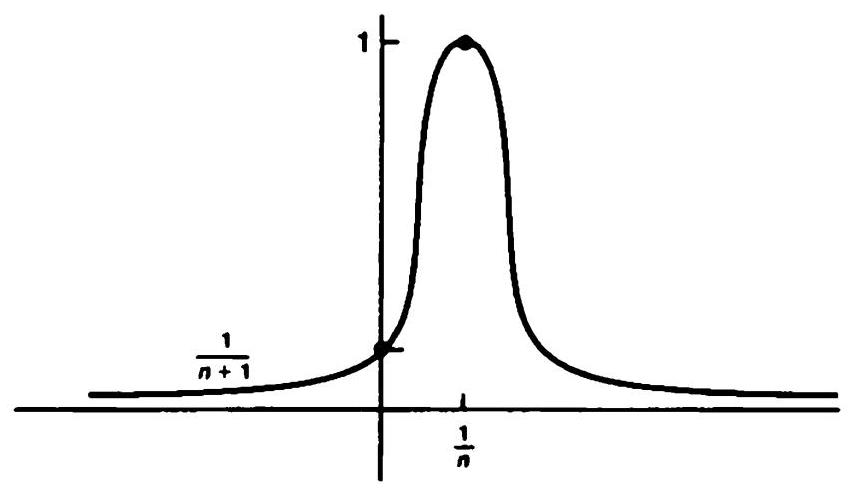
\includegraphics[width=0.7\textwidth]{images/21.1.jpg} \end{center} \hspace*{3em} Figure 21.1 The set \({B}^{2}\) is called the (closed) \index{Ball, unit} unit ball in \({\mathbb{R}}^{2}\) .
\item Prove the following standard facts about infinite series:
  \begin{enumerate}[itemsep=0.2em, parsep=0pt, topsep=0pt, partopsep=0pt, leftmargin=*, label=(\alph*), align=left]
  \item Show that if \(( {s}_{n})\) is a bounded sequence of real numbers and \({s}_{n} \leq  {s}_{n + 1}\) for each \(n\) , then \(( {s}_{n})\) converges.
  \item Let \(( {a}_{n})\) be a sequence of real numbers; define \[ {s}_{n} = \mathop{\sum }\limits_{{i = 1}}^{n}{a}_{i} \] If \({s}_{n} \rightarrow  s\) , we say that the infinite series \[ \mathop{\sum }\limits_{{i = 1}}^{\infty }{a}_{i} \] converges to \(s\) also. Show that if \(\sum {a}_{i}\) converges to \(s\) and \(\sum {b}_{i}\) converges to \(t\) , then \(\sum ( {c{a}_{i} + {b}_{i}})\) converges to \({cs} + t\) .
  \item Prove the comparison test for infinite series: If \(| {a}_{i}|  \leq  {b}_{i}\) for each \(i\) , and if the series \(\sum {b}_{i}\) converges, then the series \(\sum {a}_{i}\) converges. [Hint: Show that the series \(\sum | {a}_{i}|\) and \(\sum {c}_{i}\) converge, where \({c}_{i} = | {a}_{i}|  + {a}_{i}\) . \(\}\)
  \item Given a sequence of functions \({f}_{n} : X \rightarrow  \mathbb{R}\) , let \[ {s}_{n}( x)  = \mathop{\sum }\limits_{{i = 1}}^{n}{f}_{i}( x) . \] Prove the \index{Weierstrass M-test} Weierstrass \(M\) -test for uniform convergence: If \(| {{f}_{i}( x) }|  \leq  {M}_{i}\) for all \(x \in  X\) and all \(i\) , and if the series \(\sum {M}_{i}\) converges, then the sequence \(( {s}_{n})\) converges uniformly to a function \(s\) . [Hint: Let \({r}_{n} = \mathop{\sum }\limits_{{i = n + 1}}^{\infty }{M}_{i}\) . Show that if \(k > n\) , then \(| {{s}_{k}( x)  - {s}_{n}( x) }|  \leq  {r}_{n}\) ; conclude that \(| {s( x)  - {s}_{n}( x) }|  \leq  {r}_{n}\) .]
  \end{enumerate}
\item Prove continuity of the algebraic operations on \(\mathbb{R}\) , as follows: Use the metric \(d( {a,b})  = | {a - b}|\) on \(\mathbb{R}\) and the metric on \({\mathbb{R}}^{2}\) given by the equation \[ \rho ( {( {x,y}) ,( {{x}_{0},{y}_{0}}) })  = \max \{  {| {x - {x}_{0}}| ,| {y - {y}_{0}}| }\}  . \]
  \begin{enumerate}[itemsep=0.2em, parsep=0pt, topsep=0pt, partopsep=0pt, leftmargin=*, label=(\alph*), align=left]
  \item Show that addition is continuous. [Hint: Given \(\epsilon\) , let \(\delta  = \epsilon /2\) and note that \[ d( {x + y,{x}_{0} + {y}_{0}})  \leq  | {x - {x}_{0}}|  + | {y - {y}_{0}}| .\rbrack \]
  \item Show that multiplication is continuous. [Hint: Given \(( {{x}_{0},{y}_{0}})\) and \(0 < \epsilon  <\) 1, let \[ {3\delta } = \epsilon /( {| {x}_{0}|  + | {y}_{0}|  + 1}) \] and note that \[ d( {{xy},{x}_{0}{y}_{0}})  \leq  | {x}_{0}| | {y - {y}_{0}}|  + | {y}_{0}| | {x - {x}_{0}}|  + | {x - {x}_{0}}| | {y - {y}_{0}}| . \]
  \item Show that the operation of taking reciprocals is a continuous map from \(\mathbb{R} - \{ 0\}\) to \(\mathbb{R}\) . [Hint: Show the inverse image of the interval(a, b)is open. Consider five cases, according as \(a\) and \(b\) are positive, negative, or zero.]
  \item Show that the subtraction and quotient operations are continuous.
  \end{enumerate}
\end{enumerate}
\section*{*§ 22 The Quotient Topology \protect\sectionDagger}

Unlike the topologies we have already considered in this chapter, the \index{quotient topology} is not a natural generalization of something you have already studied in analysis. Nevertheless, it is easy enough to motivate. One motivation comes from geometry, where one often has occasion to use ``cut-and-paste'' techniques to construct such geometric objects as surfaces. The torus (surface of a doughnut), for example, can be constructed by taking a rectangle and ``pasting'' its edges together appropriately, as in Figure 22.1. And the sphere (surface of a ball) can be constructed by taking a disc and collapsing its entire boundary to a single point; see Figure 22 2. Formalizing these constructions involves the concept of quotient topology.

\begin{center}
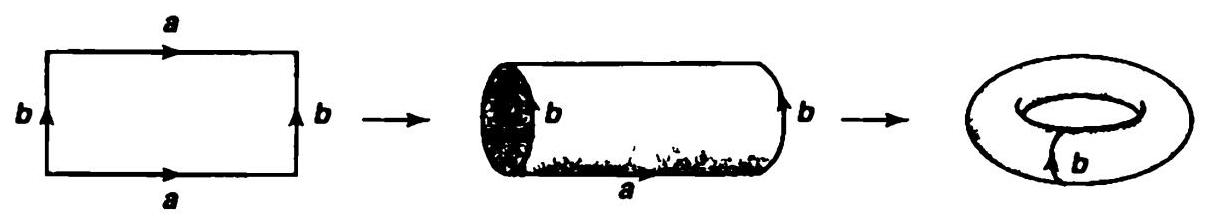
\includegraphics[width=1.0\textwidth]{images/22.1.jpg}
\end{center}
\hspace*{3em} 

Figure 22.1

\customfootnote{

${}^{\dagger}$ This section will be used throughout Part II of the book. It also is referred to in a number of exercises of Part I.

}

\begin{center}
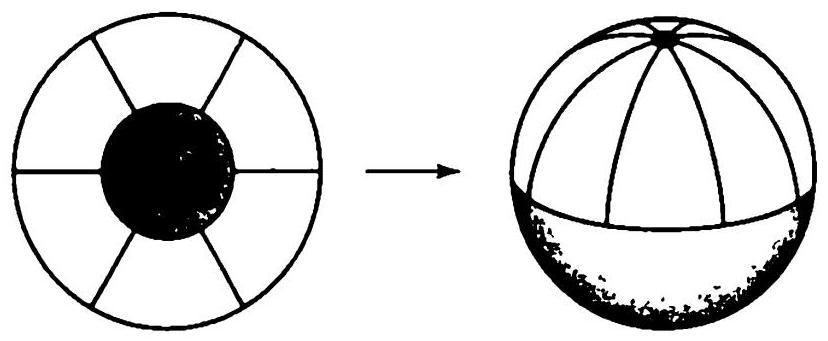
\includegraphics[width=0.7\textwidth]{images/22.2.jpg}
\end{center}
\hspace*{3em} 

Figure 22.2

\begin{definition}
	Let \(X\) and \(Y\) be topological spaces; let \(p : X \rightarrow  Y\) be a surjective map. The map \(p\) is said to be a \index{quotient map} provided a subset \(U\) of \(Y\) is open in \(Y\) if and only if \({p}^{-1}( U)\) is open in \(X\) .
\end{definition}

This condition is stronger than continuity; some mathematicians call it ``\index{strong continuity}.'' An equivalent condition is to require that a subset \(A\) of \(Y\) be closed in \(Y\) if and only if \({p}^{-1}( A)\) is closed in \(X\) . Equivalence of the two conditions follows from equation

\[
{f}^{-1}( {Y - B})  = X - {f}^{-1}( B) .
\]

Another way \index{Restriction: of a covering map!of a quotient map}of describing a \index{Quotient map}quotient map is as follows: We say that a subset \(C\) of \(X\) is \index{Saturated set} saturated (with respect to the surjective map \(p : X \rightarrow  Y\) ) if \(C\) contains every set \({p}^{-1}( {\{ y\} })\) that it intersects. Thus \(C\) is \index{saturated set@Saturated set}saturated if it equals the complete inverse image of a subset of \(Y\) . To say that \(p\) is a \index{Quotient map}quotient map is equivalent to saying that \(p\) is continuous and \(p\) maps saturated open sets of \(X\) to open sets of \(Y\) (or saturated \index{Closed set}closed sets of \(X\) to closed sets of \(Y\) ).

Two special kinds \index{Composite: of functions!of quotient maps}of quotient maps are the open maps and the \index{closed map}. Recall that a map \(f : X \rightarrow  Y\) is said to be an open map if for each open set \(U\) of \(X\) , the set \(f( U)\) is open in \(Y\) . It is said to be a closed map if for each closed set \(A\) of \(X\) , the set \(f( A)\) is closed in \(Y\) . It follows immediately from the definition that if \(p : X \rightarrow  Y\) is a surjective continuous map that is either open or closed, then \(p\) is a quotient map. There are quotient maps that are neither open nor closed. (See Exercise 3.)

\begin{centeredblock}
\begin{example}
	Let \(X\) be the subspace \([  {0,1}]   \cup  [  {2,3}]\) of \(\mathbb{R}\) , and let \(Y\) be the subspace \([  {0,2}]\) of \(\mathbb{R}\) . The map \(p : X \rightarrow  Y\) defined by

\[
p( x)  = \{  \begin{array}{ll} x & \text{ for }x \in  [  {0,1}]  , \\  x - 1 & \text{ for }x \in  [  {2,3}]   \end{array}.
\]

is readily seen to be surjective, continuous, and closed. Therefore it is a quotient map. It is not, however, an open map; the image of the open set \([  {0,1}]\) of \(X\) is not open \index{Closure!in a subspace}in \(Y\) .

Note that if \(A\) is the \index{Box topology!subspace}subspace \(\lbrack 0,1) \cup  [  {2,3}]\) of \(X\) , then the map \(q : A \rightarrow  Y\) obtained by restricting \(p\) \index{Projection map!is open map}is continuous and surjective, but it \index{Projection map!is open map}is not a quotient map. For the set \([  {2,3}]\) is open in \(A\) and is saturated with respect to \(q\) , but its image is not open in \(Y\) .
\end{example}
\end{centeredblock}

\begin{centeredblock}
\begin{example}
	Let \({\pi }_{1} : \mathbb{R} \times  \mathbb{R} \rightarrow  \mathbb{R}\) be projection onto the first coordinate; then \({\pi }_{1}\) is continuous and surjective. Furthermore, \({\pi }_{1}\) is an \index{Open map}open map. For if \(U \times  V\) is a nonempty basis element for \(\mathbb{R} \times  \mathbb{R}\) , then \({\pi }_{1}( {U \times  V})  = U\) is open in \(\mathbb{R}\) ; it follows that \({\pi }_{1}\) carries open sets of \(\mathbb{R} \times  \mathbb{R}\) to open sets of \(\mathbb{R}\) . However, \({\pi }_{1}\) is not a \index{Closed map}closed map. The subset

\[
C = \{ x \times  y \mid  {xy} = 1\}
\]

of \(\mathbb{R} \times  \mathbb{R}\) is closed, but \({\pi }_{1}( C)  = \mathbb{R} - \{ 0\}\) , which is not closed in \(\mathbb{R}\) .

Note that if \(A\) is the subspace of \(\mathbb{R} \times  \mathbb{R}\) that is the union of \(C\) and the origin \(\{ 0\}\) , then the map \(q \cdot  A \rightarrow  \mathbb{R}\) obtained by restricting \({\pi }_{1}\) is continuous and surjective, but it is not a \index{quotient map@Quotient map}quotient map. For the one-point set \(\{ \mathbf{0}\}\) is open in \(A\) and is saturated with respect to \(q\) , but its image is not open in \(\mathbb{R}\) .
\end{example}
\end{centeredblock}

Now we show how the notion of quotient map can be used to construct a topology on a set.

\begin{definition}
	If \(X\) is a space and \(A\) is a set and if \(p : X \rightarrow  A\) is a surjective map, then there exists exactly one topology \(\mathcal{T}\) on \(A\) relative to which \(p\) is a quotient map; it is called the quotient topology induced by \(p\) .
\end{definition}

The topology \(\mathcal{T}\) is of course defined by letting it consist of those subsets \(U\) of \(A\) such that \({p}^{-1}( U)\) is open in \(X\) . It is easy to check that \(\mathcal{T}\) is a topology. The sets \(\varnothing\) and \(A\) are open because \({p}^{-1}( \varnothing )  = \varnothing\) and \({p}^{-1}( A)  = X\) . The other two conditions follow from the equations

\[
{p}^{-1}( {\mathop{\bigcup }\limits_{{\alpha  \in  J}}{U}_{\alpha }})  = \mathop{\bigcup }\limits_{{\alpha  \in  J}}{p}^{-1}( {U}_{\alpha })
\]

\[
{p}^{-1}( {\mathop{\bigcap }\limits_{{i = 1}}^{n}{U}_{i}})  = \mathop{\bigcap }\limits_{{i = 1}}^{n}{p}^{-1}( {U}_{i})
\]

\begin{centeredblock}
\begin{example}
	Let \(p\) be the map of the real line \(\mathbb{R}\) onto the three-point set \(A = \{ a,b,c\}\) defined by

\[
p( x)  = \{  \begin{array}{ll} a & \text{ if }x > 0 \\  b & \text{ if }x < 0 \\  c & \text{ if }x = 0 \end{array}.
\]

You can check that the quotient topology on \(A\) induced by \(p\) is the one indicated in Figure 22.3

\begin{center}
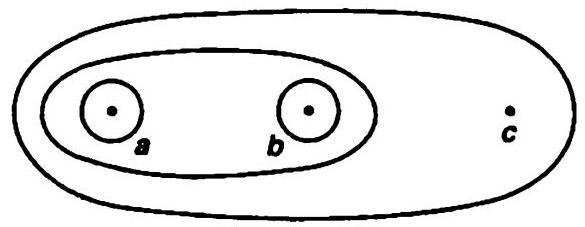
\includegraphics[width=0.5\textwidth]{images/22.3.jpg}
\end{center}
\hspace*{3em}

Figure 22.3
\end{example}
\end{centeredblock}

There is a special situation in which the quotient topology occurs particularly frequently. It is the following:

\begin{definition}
	Let \(X\) be a topological space, and let \({X}^{ * }\) be a partition of \(X\) into disjoint subsets whose union is \(X\) . Let \(p : X \rightarrow  {X}^{ * }\) be the surjective map that carries each point of \(X\) to the element of \({X}^{ * }\) containing it. In the \index{Quotient topology}quotient topology induced by \(p\) , the space \({X}^{ * }\) is called a quotient space of \(X\) .
\end{definition}

Given \({X}^{ * }\) , there is an equivalence relation on \(X\) of which the elements of \({X}^{ * }\) are the equivalence classes. One can think of \({X}^{ * }\) as having been obtained by ``ide ntifying'' each pair of equivalent points. \index{Hausdorff condition!for quotient space}For this reason, the quotient space \({X}^{ * }\) is often called an \index{identification space}, or a \index{decomposition space}, of the space \(X\) .

We can describe the topology of \({X}^{ * }\) in another way. A subset \(U\) of \({X}^{ * }\) is a collection of equivalence classes, and the set \({p}^{-1}( U)\) is just the union of the equivalence classes belongingg to \(U\) . Thus the typical open set of \({X}^{ * }\) is a collection of equivalence classes whose union is an open set of \(X\) .

\begin{centeredblock}
\begin{example}
	Let \(X\) be the closed unit ball

\[
\{  {x \times  y \mid  {x}^{2} + {y}^{2} \leq  1}\}
\]

in \({\mathbb{R}}^{2}\) , and let \({X}^{ * }\) be the partition of \(X\) consisting of all the one-point sets \(\{ x \times  y\}\) for which \({x}^{2} + {y}^{2} < 1\) , along with the set \({S}^{1} = \{ x \times  y\}  \mid  {x}^{2} + {y}^{2} = 1\}\) . Typical \index{saturated set@Saturated set}saturated open sets in \(X\) are pictured by the shaded regions in Figure 22.4. One can show that \({X}^{ * }\) is homeomorphic with the \index{Box topology!subspace}subspace of \({\mathbb{R}}^{3}\) called the unit 2-sphere, defined by

\[
\index{S@\({S}^{2}\)} {S}^{2} = \{  {( {x,y,z})  \mid  {x}^{2} + {y}^{2} + {z}^{2} = 1}\}  .
\]

\begin{center}
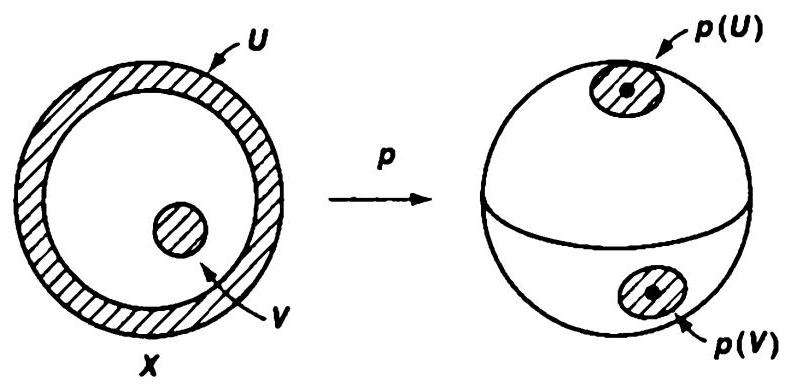
\includegraphics[width=0.7\textwidth]{images/22.4.jpg}
\end{center}
\hspace*{3em}

Figure 22.4
\end{example}
\end{centeredblock}

\begin{centeredblock}
\begin{example}
	Let \(X\) be the rectangle \([  {0,1}]   \times  [  {0,1}]\) . Define a partition \({X}^{ * }\) of \(X\) as follows: It consists of all the one-point sets \(\{ x \times  y\}\) where \(0 < x < 1\) and \(0 < y < 1\) , the following types of two-point sets:

\[
\{ x \times  0,x \times  1\} \;\text{ where }0 < x < 1,
\]

\[
\{ 0 \times  y,1 \times  y\} \;\text{ where }0 < y < 1,
\]

and the four-point set

\[
\{ 0 \times  0,0 \times  1,1 \times  0,1 \times  1\} .
\]

Typical saturated open sets in \(X\) are pictured by the shaded regions in Figure 22.5; each is an open set of \(X\) that equals a union of elements of \({X}^{ * }\) .

The image of each of these sets under \(p\) is an open set of \({X}^{ * }\) , as indicated in Figure 22.6. This description of \({X}^{ * }\) is just the mathematical way of saying what we expressed in pictures when we pasted the edges of a rectangle together to form a torus.
\end{example}
\end{centeredblock}

\begin{center}
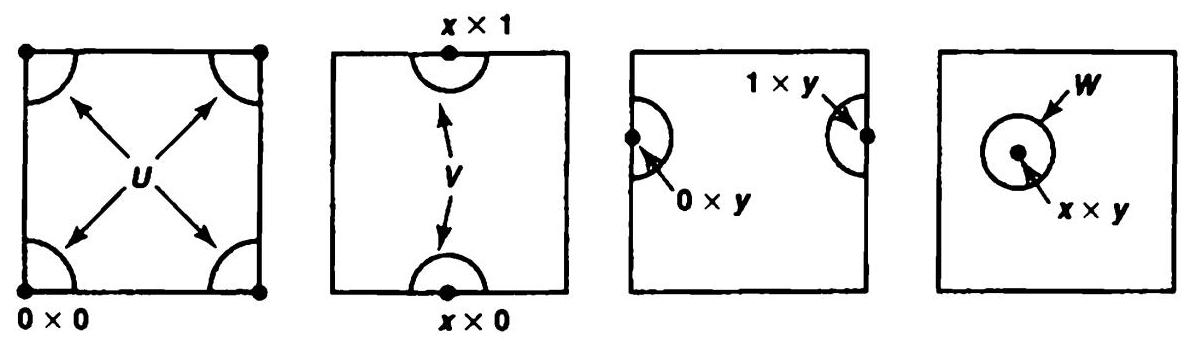
\includegraphics[width=1.0\textwidth]{images/22.5.jpg}
\end{center}
\hspace*{3em} 

Figure 22.5

\begin{center}
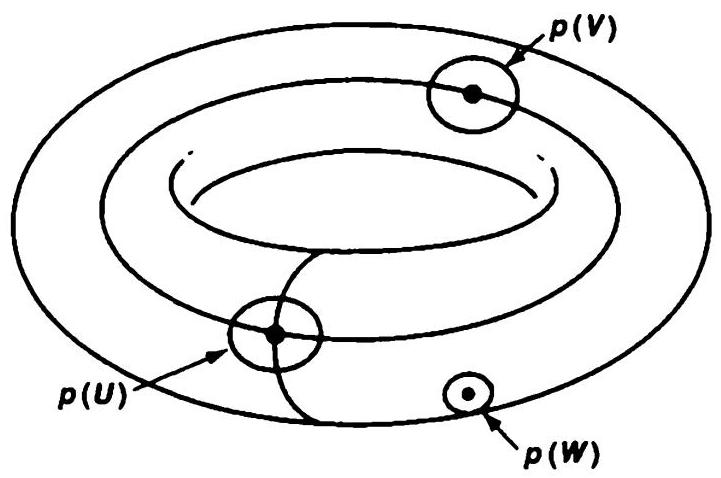
\includegraphics[width=0.6\textwidth]{images/22.6.jpg}
\end{center}
\hspace*{3em} 

Figure 22.6

Now we explore the relationship between the notions \index{Restriction: of a covering map!of a quotient map}of quotient map and quotient space and the concepts introduced previously. It is interesting to note that this relationship is not as simple as one might wish.

We have already noted that \index{Box topology!subspace}subspaces do not behave well; if \(p : X \rightarrow  Y\) is a quotient map and \(A\) is a subspace of \(X\) , then the map \(q : A \rightarrow  p( A)\) obtained by restricting \(p\) need not be a quotient map. One has, however, the following theorem:

\begin{theorem}
	Let \(p : X \rightarrow  Y\) be a quotient map; let \(A\) be a subspace of \(X\) that is saturated with respect to \(p\) ; let \(q : A \rightarrow  p( A)\) be the map obtained by restricting \(p\) .

(1) If \(A\) is either open or closed in \(X\) , then \(q\) is a quotient map.

*(2) If \(p\) is either an open map or a closed map, then \(q\) is a quotient map.

\end{theorem}
\begin{proof}
Step 1. We verify first the following two equations:

\[
{q}^{-1}( V)  = {p}^{-1}( V) \;\text{ if }V \subset  p( A)
\]

\[
p( {U \cap  A})  = p( U)  \cap  p( A) \;\text{ if }U \subset  X.
\]

To check the first equation, we note that since \(V \subset  p( A)\) and \(A\) is saturated, \({p}^{-1}( V)\) is contained in \(A\) . It follows that both \({p}^{-1}( V)\) and \({q}^{-1}( V)\) equal all points of \(A\) that are mapped by \(p\) into \(V\) . To check the second equation, we note that for any two subsets \(U\) \index{Sequences!and continuity}and \(A\) \index{Continuity: of algebraic operations in \(\mathbb{R}\)!of inclusion}of \(X\) , we have the inclusion

\[
p( {U \cap  A})  \subset  p( U)  \cap  p( A) \text{ . }
\]

To prove the reverse inclusion, suppose \(y = p( u)  = p( a)\) , for \(u \in  U\) and \(a \in  A\) . Since \(A\) is saturated, \(A\) contains the set \({p}^{-1}( {p( a) })\) , so that in particular \(A\) contains \(u\) . Then \(y = p( u)\) , where \(u \in  U \cap  A\) .

Step 2. Now suppose \(A\) is open or \(p\) is open. Given the subset \(V\) of \(p( A)\) , we assume that \({q}^{-1}( V)\) is open in \(A\) and show that \(V\) is open in \(p( A)\) .

Suppose first that \(A\) is open. Since \({q}^{-1}( V)\) is open in \(A\) and \(A\) is open in \(X\) , the set \({q}^{-1}( V)\) is open in \(X\) . Since \({q}^{-1}( V)  = {p}^{-1}( V)\) , the latter set is \index{open map@Open map}open in \(X\) , so that \(V\) is open in \(Y\) because \(p\) is a quotient map. In particular, \(V\) is open in \(p( A)\) .

Now suppose \(p\) is open. Since \({q}^{-1}( V)  = {p}^{-1}( V)\) and \({q}^{-1}( V)\) is open in \(A\) , we have \({p}^{-1}( V)  = U \cap  A\) for some set \(U\) open in \(X\) . Now \(p( {{p}^{-1}( V) })  = V\) because \(p\) is surjective; then

\[
V = p( {{p}^{-1}( V) })  = p( {U \cap  A})  = p( U)  \cap  p( A) .
\]

The set \(p( U)\) is open in \(Y\) because \(p\) is an \index{open map@Open map}open map; hence \(V\) is open in \(p( A)\) .

Step 3. The proof when \(A\) or \(p\) is closed is obtained by replacing the word ``open'' by the word ``closed'' throughout Step 2.

Now we consider other concepts introduced previously. \index{Quotient map!composites}Composites of maps behave nicely; it is easy to check that the composite of two quotient maps is a quotient map; this fact follows from the equation

\[
{p}^{-1}( {{q}^{-1}( U) })  = {( q \circ  p) }^{-1}( U) .
\]

On the other hand, \index{Quotient map!products}products of maps do not behave well; the cartesian product of two quotient maps need not be a quotient map. See Example 7 following. One needs further conditions on either the maps or the spaces in order for this statement to be true. One such, a condition on the spaces, is called local compactness; we shall study it later. Another, a condition on the maps, is the condition that both the maps \(p\) and \(q\) be open maps. In that case, it is easy to see that \(p \times  q\) is also an open map, so it is a quotient map.

Finally, the \index{Box topology!Hausdorff condition}Hausdorff condition does not behave well; even if \(X\) is Hausdorff. there is no reason that the quotient space \({X}^{ * }\) needs to be \index{Box topology!Hausdorff condition}Hausdorff. There is a simple condition for \({X}^{ * }\) to satisfy the \({T}_{1}\) axiom; one simply requires that each element of the partition \({X}^{ * }\) be a closed subset of \(X\) . Conditions that will ensure \({X}^{ * }\) is Hausdorff are harder to find. This is one of the more delicate questions concerning quotient spaces; we shall return to it several times later in the book.

Perhaps the most important result in the study of quotient spaces has to do with the problem \index{Composite: of functions!of continuous functions}of constructing continuous functions on a quotient space. We consider that problem now. When we studied \\index{Convergent sequence!in a product space}index{\index{product space@Product space}Product space}product spaces, we had a criterion for determining whether a map \(f : Z \rightarrow  \prod {X}_{\alpha }\) \index{Convergent sequence!in a product space}into a \index{product space@Product space}product space was continuous. Its counterpart in the theory of quotient spaces is a criterion for determining when a map \(f : {X}^{ * } \rightarrow  Z\) out of a quotient space is continuous. One has the following theorem:
\end{proof}

\begin{theorem}
	Let \(p : X \rightarrow  Y\) be a quotient map. Let \(Z\) be a space and let \(g : X \rightarrow  Z\) be a map that is constant on each set \({p}^{-1}( {\{ y\} })\) , for \(y \in  Y\) . Then \(g\) induces a map \(f : Y \rightarrow  Z\) such that \(f \circ  p = g\) . The induced map \(f\) is continuous if and only if \(g\) is continuous; \(f\) is a quotient map if and only if \(g\) is a quotient map.

\begin{center}
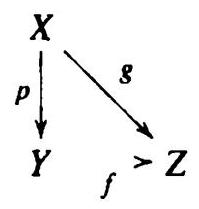
\includegraphics[width=0.2\textwidth]{images/22.7.jpg}
\end{center}
\hspace*{3em} 

\end{theorem}
\begin{proof}
For each \(y \in  Y\) , the set \(g( {{p}^{-1}( {\{ y\} }) })\) is a one-point set in \(Z\) (since \(g\) is constant on \({p}^{-1}( {\{ y\} }) )\) . If we let \(f( y)\) denote this point, then we have defined a map \(f : Y \rightarrow  Z\) such that for each \(x \in  X,f( {p( x) })  = g( x)\) . If \(f\) is continuous, then \(g = f \circ  p\) is continuous. Conversely, suppose \(g\) is continuous. Given an open set \(V\) of \(Z,{g}^{-1}( V)\) is open in \(X\) . But \({g}^{-1}( V)  = {p}^{-1}( {{f}^{-1}( V) })\) ; because \(p\) is a quotient map, it follows that \({f}^{-1}( V)\) is open in \(Y\) . Hence \(f\) is continuous.

If \(f\) is a quotient map, then \(g\) is the composite \index{Composite: of functions!of quotient maps}of two quotient maps and is thus a quotient map. Conversely, suppose that \(g\) is a quotient map. Since \(g\) is surjective, so is \(f\) . Let \(V\) be a subset of \(Z\) ; we show that \(V\) is open in \(Z\) if \({f}^{-1}( V)\) is open in \(Y\) . Now the set \({p}^{-1}( {{f}^{-1}( V) })\) is open in \(X\) because \(p\) is continuous. Since this set equals \({g}^{-1}( V)\) , the latter is open in \(X\) . Then because \(g\) is a quotient map, \(V\) is open in \(Z\) .
\end{proof}

\begin{corollary}
	Let \(g : X \rightarrow  Z\) be a surjective continuous map. Let \({X}^{ * }\) be the following collection of subsets of \(X\) :

\[
{X}^{ * } = \{  {{g}^{-1}( {\{ z\} })  \mid  z \in  Z}\}  .
\]

Give \({X}^{ * }\) the \index{Quotient topology}quotient topology.
\end{corollary}

(a) The map \(g\) induces a bijective continuous map \(f : {X}^{ * } \rightarrow  Z\) , which is a \index{Homeomorphism}homeomorphism if and only if \(g\) is a quotient map.

\begin{center}
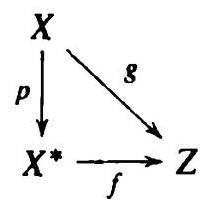
\includegraphics[width=0.2\textwidth]{images/22.8.jpg}
\end{center}
\hspace*{3em} 

(b) If \(Z\) is Hausdorff, so is \({X}^{ * }\) .

\begin{proof}
By the preceding theorem, \(g\) induces a continuous map \(f : {X}^{ * } \rightarrow  Z\) ; it is clear that \(f\) is bijective. Suppose that \(f\) is a \index{homeomorphism@Homeomorphism}homeomorphism. Then both \(f\) and the \index{Projection map}projection map \(p : X \rightarrow  {X}^{ * }\) are quotient maps, so that their composite \(q\) is a quotient map. Conversely, suppose that \(g\) is a quotient map Then it follows from the preceding theorem that \(f\) is a quotient map. Being bijective, \(f\) is thus a \index{homeomorphism@Homeomorphism}homeomorphism.

Suppose \(Z\) is Hausdorff. Given distinct pomts of \({X}^{ * }\) , their images under \(f\) are distinct and thus possess disjoint \index{Neighborhood}neighborhoods \(U\) and \(V\) . Then \({f}^{-1}( U)\) and \({f}^{-1}( V)\) are disjoint \index{neighborhood@Neighborhood}neighborhoods of the two given points of \({X}^{ * }\) .
\end{proof}

\begin{centeredblock}
\begin{example}
	Let \(X\) be the subspace of \({\mathbb{R}}^{2}\) that is the union of the line segments \([  {0,1}]   \times\)  \(\{ n\}\) , \index{Hausdorff condition!for subspace}for \(n \in  {\mathbb{Z}}_{ + }\) , and let \(Z\) be the subspace of \({\mathbb{R}}^{2}\) consisting of all points of the form \(x \times  ( {x/n})\) for \(x \in  [  {0,1}]\) and \(n \in  {\mathbb{Z}}_{ + }\) . Then \(X\) is the union of countably many disjoint line segments, and \(Z\) is the union of countably many line segments having an end point in common. See Figure 22.7.

Define a map \(g : X \rightarrow  Z\) by the equation \(g( {x \times  n})  = x \times  ( {x/n})\) ; then \(g\) is surjective and continuous. The quotient space \({X}^{ * }\) whose elements are the sets \({g}^{-1}( {\{ z\} })\) is simply the space obtained from \(X\) by identifying the subset \(\{ 0\}  \times  {\mathbb{Z}}_{ + }\) to a point. The map \(g\) induces a bijective continuous map \(f : {X}^{ * } \rightarrow  Z\) . But \(f\) is not a homeomorphism.

To verify this fact, it suffices to show that \(g\) is not a quotient map. Consider the sequence of points \({x}_{n} = ( {1/n})  \times  n\) of \(X\) . The set \(A = \{  {x}_{n}\}\) is a closed subset of \(X\) because it has no limut points. Also, it is saturated with respect to \(g\) On the other hand, the set \(g( A)\) is not closed in \(Z\) , for it consists of the points \({z}_{n} = ( {1/n})  \times  ( {1/{n}^{2}})\) ; this set has the origin as a \index{Limit point}limit point.

\begin{center}
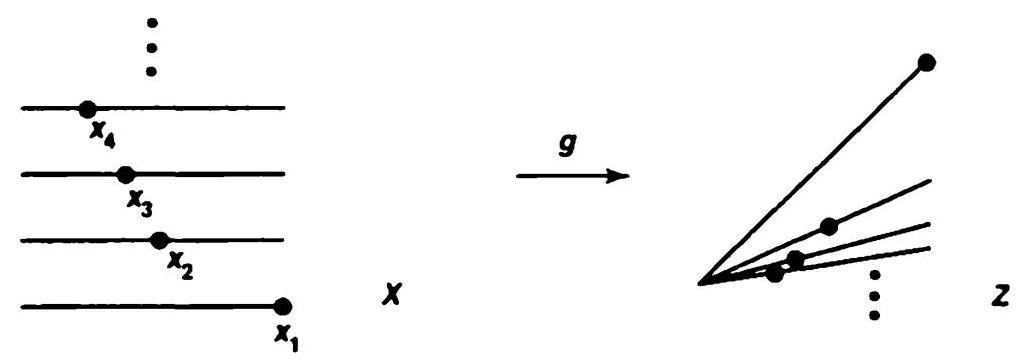
\includegraphics[width=0.9\textwidth]{images/22.9.jpg}
\end{center}
\hspace*{3em}

Figure 22.7
\end{example}
\end{centeredblock}

\begin{centeredblock}
\begin{example}
	The product of two quotient maps need not be a quotient map

We give an example that involves non-Hausdorff spaces in the exercises. Here is another involving spaces that are nicer.

Let \(X = \mathbb{R}\) and let \({X}^{ * }\) be the quotient space obtained from \(X\) by identifying the subset \({\mathbb{Z}}_{ + }\) to a point \(b\) ; let \(p : X \rightarrow  {X}^{ * }\) be the quotient map. Let \(\mathbb{Q}\) be the subspace of \(\mathbb{R}\) consisting of the rational numbers; let \(i : \mathbb{Q} \rightarrow  \mathbb{Q}\) be the identity map. We show that

\[
p \times  i : X \times  \mathbb{Q} \rightarrow  {X}^{ * } \times  \mathbb{Q}
\]

is not a quotient map.

For each \(n\) , let \({c}_{n} = \sqrt{2}/n\) , and c\index{Standard topology: on \(\mathbb{R}\)!on \({\mathbb{R}}^{2}\)}\index{Standard topology: on \(\mathbb{R}\)!on \({\mathbb{R}}^{2}\)}onsider the straight lines in \({\mathbb{R}}^{2}\) with slopes 1 and -1, respectively, through the point \(n \times  {c}_{n}\) Let \({U}_{n}\) consist of all points of \(X \times  \mathbb{Q}\) that lie above both of these lines or beneath both of them, and also between the vertical lines \(x = n - 1/4\) and \(x = n + 1/4\) . Then \({U}_{n}\) is open in \(X \times  \mathbb{Q}\) ; it contains the set \(\{ n\}  \times  \mathbb{Q}\) because \({c}_{n}\) is not rational. See Figure 22.8

Let \(U\) be the union of the sets \({U}_{n}\) ; then \(U\) is open in \(X \times  \mathbb{Q}\) . It is saturated with respect to \(p \times  i\) because it contains the enture set \({\mathbb{Z}}_{ + } \times  \{ q\}\) for each \(q \in  \mathbb{Q}\) . We assume that \({U}^{\prime } = ( {p \times  i}) ( U)\) is open in \({X}^{ * } \times  \mathbb{Q}\) and derive a contradiction

Because \(U\) contains, in particular, the set \({\mathbb{Z}}_{ + } \times  0\) , the set \({U}^{\prime }\) contains the point \(b \times  0\) . Hence \({U}^{\prime }\) contains an open set of the form \(W \times  {I}_{\delta }\) , where \(W\) is a \index{neighborhood@Neighborhood}neighborhood of \(b\) in \({X}^{ * }\) and \({l}_{\delta }\) consists of all rational numbers \(y\) with \(| y|  < \delta\) . Then

\[
{p}^{-1}( W)  \times  {I}_{\delta } \subset  U
\]

Choose \(n\) large enough that \({c}_{n} < \delta\) . Then since \({p}^{-1}( W)\) is open in \(X\) and contains \({\mathbb{Z}}_{ + }\) , we can choose \(\epsilon  < 1/4\) so that the interval \(( {n - \epsilon ,n + \epsilon })\) is contained in \({p}^{-1}( W)\) . Then \(U\) contains the subset \(V = ( {n - \epsilon ,n + \epsilon })  \times  {I}_{\delta }\) of \(X \times  \mathbb{Q}\) . But the figure makes clear that there are many points \(x \times  y\) of \(V\) that do not lie in \(U\) ! (One such is the point \(x \times  y\) , where \(x = n + \frac{1}{2}\epsilon\) and \(y\) is a rational number with \(| {y - {c}_{n}}|  < \frac{1}{2}\epsilon\) )

\begin{center}
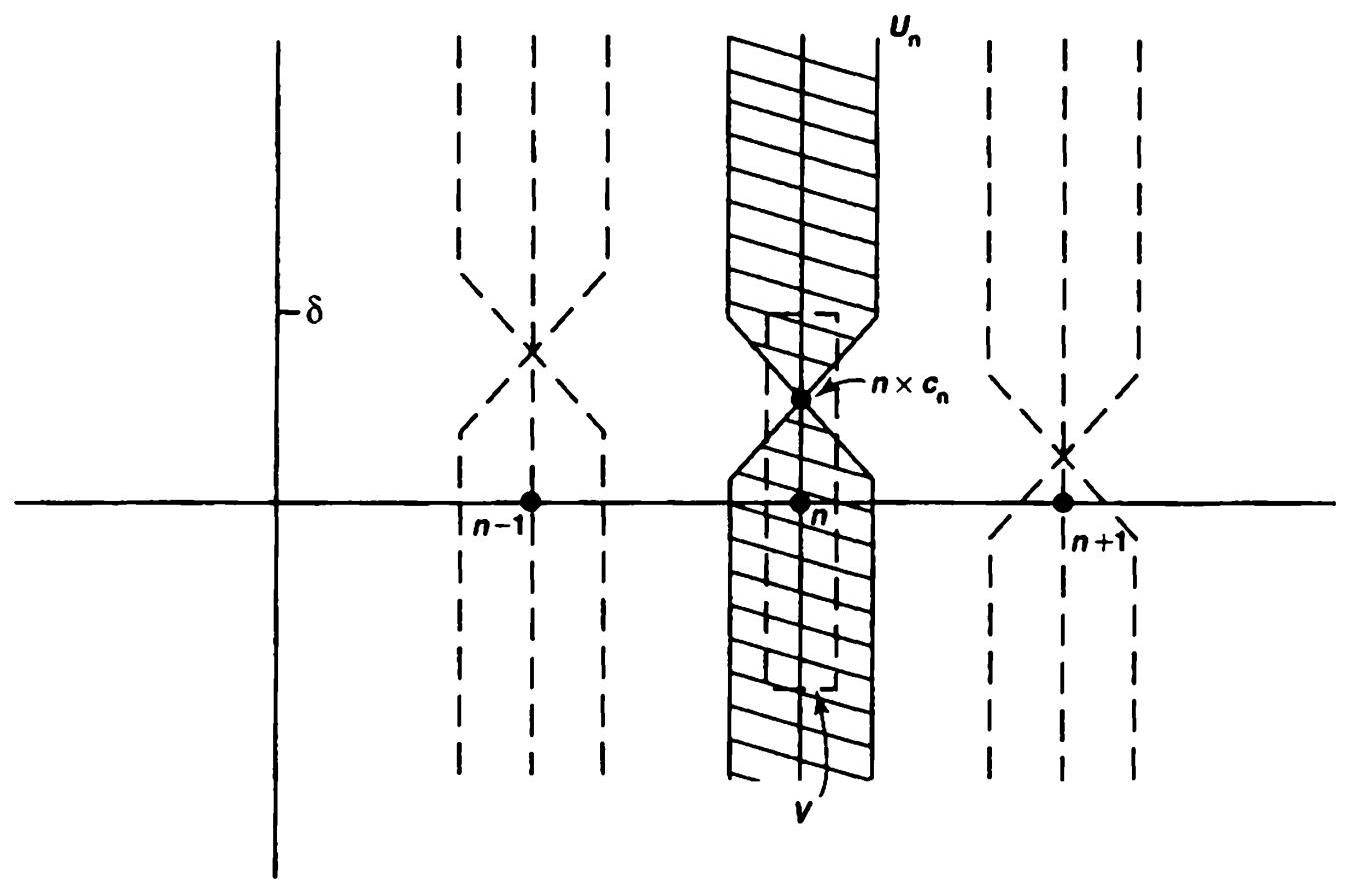
\includegraphics[width=1.0\textwidth]{images/22.10.jpg}
\end{center}
\hspace*{3em}

Figure 22.8
\end{example}
\end{centeredblock}

\section*{Exercises}
\begin{enumerate}[itemsep=0.4em, parsep=0pt, topsep=0pt, partopsep=0pt, leftmargin=*, label=\arabic*., ref=\arabic*]
\item Check the details of Example 3.
\item
  \begin{enumerate}[itemsep=0.2em, parsep=0pt, topsep=0pt, partopsep=0pt, leftmargin=*, label=(\alph*), align=left]
  \item Let \(p : X \rightarrow  Y\) be a continuous map. Show that if there is a continuous map \(f : Y \rightarrow  X\) such that \(p \circ  f\) equals the identity map of \(Y\) , then \(p\) is a quotient map.

  \item If \(A \subset  X\) , a retraction of \(X\) onto \(A\) is a continuous map \(r : X \rightarrow  A\) such that \(r( a)  = a\) for each \(a \in  A\) . Show that a retraction is a quotient map.
  \end{enumerate}
\item Let \({\pi }_{1} : \mathbb{R} \times  \mathbb{R} \rightarrow  \mathbb{R}\) be projection on the first coordinate Let \(A\) be the subspace of \(\mathbb{R} \times  \mathbb{R}\) consisting of all points \(x \times  y\) for which either \(x \geq  0\) or \(y = 0\) (or both); let \(q : A \rightarrow  \mathbb{R}\) be obtained by restricting \({\pi }_{1}\) . Show that \(q\) is a quotient map that is neither open nor closed.
\item
  \begin{enumerate}[itemsep=0.2em, parsep=0pt, topsep=0pt, partopsep=0pt, leftmargin=*, label=(\alph*), align=left]
  \item Define an equivalence relation on the plane \(X = {\mathbb{R}}^{2}\) as follows: \[ {x}_{0} \times  {y}_{0} \sim  {x}_{1} \times  {y}_{1}\;\text{ if }{x}_{0} + {y}_{0}^{2} = {x}_{1} + {y}_{1}^{2}. \] Let \({X}^{ * }\) be the corresponding quotient space. It is homeomorphic to a familiar space; what is it? [Hint: Set \(g( {x \times  y})  = x + {y}^{2}\) .]

  \item Repeat (a) for the equivalence relation \[ {x}_{0} \times  {y}_{0} \sim  {x}_{1} \times  {y}_{1}\;\text{ if }{x}_{0}^{2} + {y}_{0}^{2} = {x}_{1}^{2} + {y}_{1}^{2}. \]
  \end{enumerate}
\item Let \(p : X \rightarrow  Y\) be an open map. Show that if \(A\) is open in \(X\) , then the map \(q : A \rightarrow  p( A)\) obtained by restricting \(p\) is an open map.
\item Recall that \({\mathbb{R}}_{K}\) denotes the real line in the \(K\) -topology. (See \(§{13}\) .) Let \(Y\) be the quotient space obtained from \({\mathbb{R}}_{K}\) by collapsing the set \(K\) to a point; let \(p : {\mathbb{R}}_{K} \rightarrow  Y\) be the quotient map.
  \begin{enumerate}[itemsep=0.2em, parsep=0pt, topsep=0pt, partopsep=0pt, leftmargin=*, label=(\alph*), align=left]
  \item Show that \(Y\) satisfies the \({T}_{1}\) axiom, but is not Hausdorff.
  \item Show that \(p \times  p.{\mathbb{R}}_{K} \times  {\mathbb{R}}_{K} \rightarrow  Y \times  Y\) is not a quotient map. [Hint: The \index{Diagonal}diagonal is not closed in \(Y \times  Y\) , but its inverse image is closed in \({\mathbb{R}}_{K} \times  {\mathbb{R}}_{K}\) .]
  \end{enumerate}
\end{enumerate}
\section*{* Supplementary Exercises: Topological Groups}

In these exercises we consider topological groups and some of their properties. The quotient topology gets its name from the special case that arises when one forms the quotient of a topological group by a subgroup.

A topological group \(G\) is a group that is also a topological space satisfying the \({T}_{1}\) axiom, such that the map of \(G \times  G\) into \(G\) sending \(x \times  y\) into \(x \cdot  y\) , and the map of \(G\) into \(G\) sending \(x\) into \({x}^{-1}\) , are continuous maps. Throughout the following exercises, let \(G\) denote a topological group.

1. Let \(H\) denote a group that is also a topological space satisfying the \({T}_{1}\) axiom. Show that \(H\) is a topological group if and only if the map of \(H \times  H\) into \(H\) sending \(x \times  y\) into \(x \cdot  {y}^{-1}\) is continuous.

2. Show that the following are topological groups:

(a) \(( {\mathbb{Z}, + })\)

(b) \(( {\mathbb{R}, + })\)

(c) \(( {{\mathbb{R}}_{ + }, \cdot  })\)

(d) \(( {{S}^{1}, \cdot  })\) , where we take \({S}^{1}\) to be the space of all complex numbers \(z\) for which \(| z|  = 1\) .

(e) The general linear group \(\mathrm{{GL}}( n)\) , under the operation of matrix multiplication. (GL(n)is the set of all nonsingular \(n\) by \(n\) matrices, topologized by considering it as a subset of euclidean space of dimension \({n}^{2}\) in the obvious way.)

3. Let \(H\) be a subspace of \(G\) . Show that if \(H\) is also a subgroup of \(G\) , then both \(H\) and \(\bar{H}\) are topological groups.

4. Let \(\alpha\) be an element of \(G\) . Show that the maps \({f}_{\alpha },{g}_{\alpha } : G \rightarrow  G\) defined by

\[
{f}_{\alpha }( x)  = \alpha  \cdot  x\;\text{ and }\;{g}_{\alpha }( x)  = x \cdot  \alpha
\]

are homeomorphisms of \(G\) . Conclude that \(G\) is a homogeneous space. (This means that for every pair \(x,y\) of points of \(G\) , there exists a homeomorphism of \(G\) onto itself that carries \(x\) to \(y\) .)

5. Let \(H\) be a subgroup of \(G\) . If \(x \in  G\) , define \({xH} = \{ x \cdot  h \mid  h \in  H\}\) ; this set is called a left coset of \(H\) in \(G\) . Let \(G/H\) denote the collection of left cosets of \(H\) in \(G\) ; it is a partition of \(G\) . Give \(G/H\) the \index{quotient topology@Quotient topology}quotient topology.

(a) Show that if \(\alpha  \in  G\) , the map \({f}_{\alpha }\) of the preceding exercise induces a homeomorphism of \(G/H\) carrying \({xH}\) to \(( {\alpha  \cdot  x}) H\) . Conclude that \(G/H\) is a homogeneous space.

(b) Show that if \(H\) is a \index{closed set@Closed set}closed set in the topology of \(G\) , then one-point sets are \index{closed map@Closed map}closed in \(G/H\) .

(c) Show that the quotient map \(p : G \rightarrow  G/H\) is open.

(d) Show that if \(H\) is closed in the topology of \(G\) and is a \index{Norm}normal subgroup of \(G\) , then \(G/H\) is a topological group.

6. The integers \(\mathbb{Z}\) are a normal subgroup of \(( {\mathbb{R}, + })\) . The quotient \(\mathbb{R}/\mathbb{Z}\) is a familiar topological group; what is it?

7. If \(A\) and \(B\) are subsets of \(G\) , let \(A \cdot  B\) denote the set of all points \(a \cdot  b\) for \(a \in  A\) and \(b \in  B\) . Let \({A}^{-1}\) denote the set of all points \({a}^{-1}\) , for \(a \in  A\) .

(a) A neighborhood \(V\) of the identity element \(e\) is said to be sym\index{Metric}metric if \(V =\)  \({V}^{-1}\) . If \(U\) is a neighborhood of \(e\) , show there is a sym\index{metric@Metric}metric neighborhood \(V\) of \(e\) such that \(V \cdot  V \subset  U\) . [Hint: If \(W\) is a neighborhood of \(e\) , then \(W \cdot  {W}^{-1}\) is symmetric.]

(b) Show that \(G\) is Hausdorff. In fact, show that if \(x \neq  y\) , there is a neighborhood \(V\) of \(e\) such that \(V \cdot  x\) and \(V \cdot  y\) are disjoint.

(c) Show that \(G\) satisfies the following separation axiom, which is called the regularity axiom: Given a \index{closed set@Closed set}closed set \(A\) and a point \(x\) not in \(A\) , there exist disjoint open sets containing \(A\) and \(x\) , respectively. [Hint: There is a neighborhood \(V\) of \(e\) such that \(V \cdot  x\) and \(V \cdot  A\) are disjoint.]

(d) Let \(H\) be a subgroup of \(G\) that is closed in the topology of \(G\) ; let \(p : G \rightarrow\)  \(G/H\) be the quotient map. Show that \(G/H\) satisfies the regularity axiom. [Hint. Examine the proof of (c) when \(A\) is saturated.]
\chapter{Connectedness and Compactness}

In the study of calculus, there are three basic theorems about continuous functions, and on these theorems the rest of calculus depends. They are the following:

Intermediate value theorem. If \(f: \left\lbrack {a,b}\right\rbrack \rightarrow \mathbb{R}\) is continuous and if \(r\) is a real number between \(f\left( a\right)\) and \(f\left( b\right)\) , then there exists an element \(c \in \left\lbrack {a,b}\right\rbrack\) such that \(f\left( c\right) = r\) .

Maximum value theorem. If \(f: \left\lbrack {a,b}\right\rbrack \rightarrow R\) is continuous, then there exists an element \(c \in \left\lbrack {a,b}\right\rbrack\) such that \(f\left( x\right) \leq f\left( c\right)\) for every \(x \in \left\lbrack {a,b}\right\rbrack\) .

Uniform continuity theorem. If \(f: \left\lbrack {a,b}\right\rbrack \rightarrow \mathbb{R}\) is continuous, then given \(\epsilon > 0\) , there exists \(\delta > 0\) such that \(\left| {f\left( {x}_{1}\right) - f\left( {x}_{2}\right) }\right| < \epsilon\) for every pair of numbers \({x}_{1},{x}_{2}\) of \(\left\lbrack {a,b}\right\rbrack\) for which \(\left| {{x}_{1} - {x}_{2}}\right| < \delta\) .

These theorems are used in a number of places. The intermediate value theorem is used for instance in constructing inverse functions, such as \(\sqrt[3]{x}\) and arcsin \(x\) ; and the maximum value theorem is used for proving the mean value theorem for derivatives, upon which the two fundamental theorems of calculus depend. The uniform continuity theorem is used, among other things, for proving that every continuous function is integrable.

We have spoken of these three theorems as theorems about continuous functions. But they can also be considered as theorems about the closed interval \(\left\lbrack {a,b}\right\rbrack\) of real numbers. The theorems depend not only on the continuity of \(f\) but also on properties of the topological space \(\left\lbrack {a,b}\right\rbrack\) .

The property of the space \(\left\lbrack {a,b}\right\rbrack\) on which the intermediate value theorem depends is the property called connectedness, and the property on which the other two depend is the property called compactness. In this chapter, we shall define these properties for arbitrary topological spaces, and shall prove the appropriate generalized versions of these theorems.

As the three quoted theorems are fundamental for the theory of calculus, so are the notions of connectedness and compactness fundamental in higher analysis, geometry, and topology-indeed, in almost any subject for which the notion of topological space itself is relevant.

\section*{§ 23 Connected Spaces}

The definition of connectedness for a topological space is a quite natural one. One says that a space can be ``separated'' if it can be broken up into two ``globs''—disjoint open sets. Otherwise, one says that it is connected. From this simple idea much follows.

\begin{definition} Let \(X\) be a topological space. A separation of \(X\) is a pair \(U,V\) of disjoint nonempty open subsets of \(X\) whose union is \(X\) . The space \(X\) is said to be connected if there does not exist a separation of \(X\) .
\end{definition}


Connectedness is obviously a topological property, since it is formulated entirely in terms of the collection of open sets of \(X\) . Said differently, if \(X\) is connected, so is any space homeomorphic to \(X\) .

Another way of formulating the definition of connectedness is the following:

A space \(X\) is connected if and only if the only subsets of \(X\) that are both open and closed in \(X\) are the empty set and \(X\) itself.

For if \(A\) is a nonempty proper subset of \(X\) that is both open and closed in \(X\) , then the sets \(U = A\) and \(V = X - A\) constitute a separation of \(X\) , for they are open, disjoint, and nonempty, and their union is \(X\) . Conversely, if \(U\) and \(V\) form a separation of \(X\) , then \(U\) is nonempty and different from \(X\) , and it is both open and closed in \(X\) .

For a subspace \(Y\) of a topological space \(X\) , there is another useful way of formulating the definition of connectedness:

\begin{lemma} If \(Y\) is a subspace of \(X\) , a separation of \(Y\) is a pair of disjoint nonempty sets \(A\) and \(B\) whose union is \(Y\) , neither of which contains a limit point of the other. The space \(Y\) is connected if there exists no separation of \(Y\) .
\end{lemma}

\begin{proof}
Suppose first that \(A\) and \(B\) form a separation of \(Y\) . Then \(A\) is both open and closed in \(Y\) . The closure of \(A\) in \(Y\) is the set \(\bar{A} \cap Y\) (where \(\bar{A}\) as usual denotes the closure of \(A\) in \(X\) ). Since \(A\) is closed in \(Y,A = \bar{A} \cap Y\) ; or to say the same thing, \(\bar{A} \cap B = \varnothing\) . Since \(A\) is the union of \(A\) and its limit points, \(B\) contains no limit points of \(A\) . A similar argument shows that \(A\) contains no limit points of \(B\) .

Conversely, suppose that \(A\) and \(B\) are disjoint nonempty sets whose union is \(Y\) , neither of which contains a limit point of the other. Then \(\bar{A} \cap B = \varnothing\) and \(A \cap \bar{B} = \varnothing\) ; therefore, we conclude that \(\bar{A} \cap Y = A\) and \(\bar{B} \cap Y = B\) . Thus both \(A\) and \(B\) are closed in \(Y\) , and since \(A = Y - B\) and \(B = Y - A\) , they are open in \(Y\) as well.
\end{proof}

\begin{centeredblock}
\begin{example} Let \(X\) denote a two-point space in the indiscrete topology. Obviously there is no separation of \(X\) , so \(X\) is connected.
\end{example}
\end{centeredblock}

\begin{centeredblock}
\begin{example} Let \(Y\) denote the subspace \(\left\lbrack {-1,0)\cup (0,1}\right\rbrack\) of the real line \(\mathbb{R}\) . Each of the sets \(\left\lbrack {-1,0)\text{ and }(0,1}\right\rbrack\) is nonempty and open in \(Y\) (although not in \(\mathbb{R}\) ); therefore, they form a separation of \(Y\) . Alternatively, note that neither of these sets contains a limit point of the other. (They do have a limit point 0 in common, but that does not matter.)
\end{example}
\end{centeredblock}

\begin{centeredblock}
\begin{example} Let \(X\) be the subspace \(\left\lbrack {-1,1}\right\rbrack\) of the real line. The sets \(\left\lbrack {-1,0}\right\rbrack\) and \((0,1\rbrack\) are disjoint and nonempty, but they do not form a separation of \(X\) , because the first set is not open in \(X\) . Alternatively, note that the first set contains a limit point,0, of the second. Indeed, there exists \(n\) o separation of the space \(\left\lbrack {-1,1}\right\rbrack\) . We shall prove this fact shortly
\end{example}
\end{centeredblock}

\begin{centeredblock}
\begin{example} The rationals \(\mathbb{Q}\) are not connected. Indeed, the only connected subspaces of \(\mathbb{Q}\) are the one-point sets \(\cdot\) If \(Y\) is a subspace of \(\mathbb{Q}\) containing two points \(p\) and \(q\) , one can choose an irrational number a lying between \(p\) and \(q\) , and write \(Y\) as the union of the open sets

\[
Y \cap \left( {-\infty,a}\right) \;\text{ and }\;Y \cap \left( {a, + \infty }\right) .
\]
\end{example}
\end{centeredblock}

\begin{centeredblock}
\begin{example} Consider the following subset of the plane \({\mathbb{R}}^{2}\) :

\[
X = \{ x \times y \mid y = 0\} \cup \{ x \times y \mid x > 0\text{ and }y = 1/x\} .
\]

Then \(X\) is not connected, indeed, the two indicated sets form a separation of \(X\) because neither contains a limit point of the other. See Figure 23.1.

\begin{center}
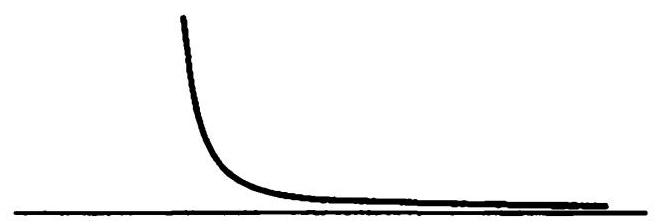
\includegraphics[width=0.6\textwidth]{images/23.1.jpg}
\end{center}
\hspace*{3em}

Figure 23.1
\end{example}
\end{centeredblock}

We have given several examples of spaces that are not connected. How can one construct spaces that are connected? We shall now prove several theorems that tell how to form new connected spaces from given ones. In the next section we shall apply these theorems to show that some specific spaces, such as intervals in \(\mathbb{R}\) , and balls and cubes in \({\mathbb{R}}^{n}\) , are connected. First, a lemma:

\begin{lemma} If the sets \(C\) and \(D\) form a separation of \(X\) , and if \(Y\) is a connected subspace of \(X\) , then \(Y\) lies entirely within either \(C\) or \(D\) .
\end{lemma}

\begin{proof}
Since \(C\) and \(D\) are both open in \(X\) , the sets \(C \cap Y\) and \(D \cap Y\) are open in \(Y\) . These two sets are disjoint and their union is \(Y\) ; if they were both nonempty, they would constitute a separation of \(Y\) . Therefore, one of them is empty. Hence \(Y\) must lie entirely in \(C\) or in \(D\)
\end{proof}

\begin{theorem} The union of a collection of connected subspaces of \(X\) that have a point in common is connected.

\end{theorem}
Proof. Let \(\left\{ {A}_{\alpha }\right\}\) be a collection of connected subspaces of a space \(X\) ; let \(p\) be a point of \(\bigcap {A}_{\alpha }\) . We prove that the space \(Y = \bigcup {A}_{\alpha }\) is connected. Suppose that \(Y = C \cup D\) is a separation of \(Y\) . The point \(p\) is in one of the sets \(C\) or \(D\) ; suppose \(p \in C\) . Since \({A}_{\alpha }\) is connected, it must lie entirely in either \(C\) or \(D\) , and it cannot lie in \(D\) because it contains the point \(p\) of \(C\) . Hence \({A}_{\alpha } \subset C\) for every \(\alpha\) , so that \(\bigcup {A}_{\alpha } \subset C\) , contradicting the fact that \(D\) is nonempty.

\begin{theorem} Let \(A\) be a connected subspace of \(X\) . If \(A \subset B \subset \bar{A}\) , then \(B\) is also connected.

Said differently: If \(B\) is formed by adjoining to the connected subspace \(A\) some or all of its limit points, then \(B\) is connected.

\end{theorem}
\begin{proof} Let \(A\) be connected and let \(A \subset B \subset \bar{A}\) . Suppose that \(B = C \cup D\) is a separation of \(B\) . By Lemma 23.2, the set \(A\) must lie entirely in \(C\) or in \(D\) ; suppose that \(A \subset C\) . Then \(\widetilde{A} \subset \widetilde{C}\) ; since \(\widetilde{C}\) and \(D\) are disjoint, \(B\) cannot intersect \(D\) . This contradicts the fact that \(D\) is a nonempty subset of \(B\) .
\end{proof}

\begin{theorem} The image of a connected space under a continuous map is connected.

\end{theorem}
\begin{proof} Let \(f: X \rightarrow Y\) be a continuous map; let \(X\) be connected. We wish to prove the image space \(Z = f\left( X\right)\) is connected. Since the map obtained from \(f\) by restricting its range to the space \(Z\) is also continuous, it suffices to consider the case of a continuous surjective map

\[
g: X \rightarrow Z\text{ . }
\]

Suppose that \(Z = A \cup B\) is a separation of \(Z\) into two disjoint nonempty sets open in \(Z\) . Then \({g}^{-1}\left( A\right)\) and \({g}^{-1}\left( B\right)\) are disjoint sets whose union is \(X\) ; they are open in \(X\) because \(g\) is continuous, and nonempty because \(g\) is surjective. Therefore, they form a separation of \(X\) , contradicting the assumption that \(X\) is connected.
\end{proof}

\section*{Theorem 23.6. A finite cartesian product of connected spaces is connected.}

\begin{proof}
We prove the theorem first for the product of two connected spaces \(X\) and \(Y\) . This proof is easy to visualize. Choose a ``base point'' \(a \times b\) in the product \(X \times Y\) . Note that the ``horizontal slice'' \(X \times b\) is connected, being homeomorphic with \(X\) , and each ``vertical slice'' \(x \times Y\) is connected, being homeomorphic with \(Y\) . As a result, each ``T-shaped'' space

\[
{T}_{x} = \left( {X \times b}\right) \cup \left( {x \times Y}\right)
\]

is connected, being the union of two connected spaces that have the point \(x \times b\) in common. See Figure 23.2. Now form the union \(\mathop{\bigcup }\limits_{{x \in X}}{T}_{x}\) of all these T-shaped spaces. This union is connected because it is the union of a collection of connected spaces that have the point \(a \times b\) in common. Since this union equals \(X \times Y\) , the space \(X \times Y\) is connected.

\begin{center}
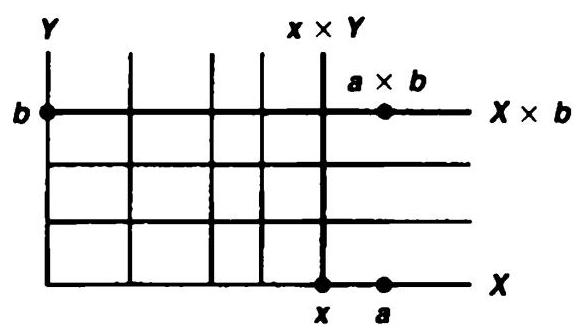
\includegraphics[width=0.5\textwidth]{images/23.2.jpg}
\end{center}
\hspace*{3em} 

Figure 23.2

The proof for any finite product of connected spaces follows by induction, using the fact (easily proved) that \({X}_{1} \times \cdots \times {X}_{n}\) is homeomorphic with \(\left( {{X}_{1} \times \cdots \times {X}_{n - 1}}\right) \times\) \({X}_{n}\) .

It is natural to ask whether this theorem extends to arbitrary products of connected spaces. The answer depends on which topology is used for the product, as the following examples show.
\end{proof}

\begin{centeredblock}
\begin{example} Consider the cartesian product \({\mathbb{R}}^{\omega }\) in the box topology. We can write \({\mathbb{R}}^{\omega }\) as the union of the set \(A\) consisting of all bounded sequences of real numbers, and the set \(B\) of all unbounded sequences. These sets are disjoint, and each is open in the box topology For if \(\mathbf{a}\) is a point of \({\mathbb{R}}^{\omega }\) , the open set

\[
U = \left( {{a}_{1} - 1,{a}_{1} + 1}\right) \times \left( {{a}_{2} - 1,{a}_{2} + 1}\right) \times
\]

consists enturely of bounded sequences if \(a\) is bounded, and of unbounded sequences if \(a\) if unbounded. Thus, even though \(\mathbb{R}\) is connected (as we shall prove in the next section), \({\mathbb{R}}^{\omega }\) is not connected in the box topology.
\end{example}
\end{centeredblock}

\begin{centeredblock}
\begin{example} Now consider \({\mathbb{R}}^{\omega }\) in the product topology. Assuming that \(\mathbb{R}\) is connected, we show that \({\mathbb{R}}^{\omega }\) is connected. Let \({\overline{\mathbb{R}}}^{n}\) denote the subspace of \({\mathbb{R}}^{\omega }\) consisting of all sequences \(\mathbf{x} = \left( {{x}_{1},{x}_{2},\ldots }\right)\) such that \({x}_{i} = 0\) for \(i > n\) The space \({\overline{\mathbb{R}}}^{n}\) is clearly homeomorphic to \({\mathbb{R}}^{n}\) , so that it is connected, by the preceding theorem. It follows that the space \({\mathbb{R}}^{\infty }\) that is the union of the spaces \({\overline{\mathbb{R}}}^{n}\) is connected, for these spaces have the point \(\mathbf{0} = \left( {0,0,\ldots }\right)\) in common. We show that the closure of \({\mathbb{R}}^{\infty }\) equals all of \({\mathbb{R}}^{\omega }\) , from which it follows that \({\mathbb{R}}^{\omega }\) is connected as well.

Let \(\mathbf{a} = \left( {{a}_{1},{a}_{2},\ldots }\right)\) be a point of \({\mathbb{R}}^{\omega }\) . Let \(U = \prod {U}_{i}\) be a basis element for the product topology that contains a. We show that \(U\) intersects \({\mathbb{R}}^{\infty }\) . There is an integer \(N\) such that \({U}_{i} = \mathbb{R}\) for \(i > N\) . Then the point

\[
\mathbf{x} = \left( {{a}_{1},\ldots,{a}_{n},0,0,\;}\right)
\]

of \({\mathbb{R}}^{\infty }\) belongs to \(U\) , since \({a}_{i} \in {U}_{i}\) for all \(i\) , and \(0 \in {U}_{i}\) for \(i > N\) .
\end{example}
\end{centeredblock}

The argument just given generalizes to show that an arbitrary product of connected spaces is connected in the product topology. Since we shall not need this result, we leave the proof to the exercises.

\section*{Exercises}

1. Let \(\mathcal{T}\) and \({\mathcal{T}}^{\prime }\) be two topologies on \(X\) . If \({\mathcal{T}}^{\prime } \supset \mathcal{T}\) , what does connectedness of \(X\) in one topology imply about connectedness in the other?

2. Let \(\left\{ {A}_{n}\right\}\) be a sequence of connected subspaces of \(X\) , such that \({A}_{n} \cap {A}_{n + 1} \neq \varnothing\) for all \(n\) . Show that \(\bigcup {A}_{n}\) is connected.

3. Let \(\left\{ {A}_{\alpha }\right\}\) be a collection of connected subspaces of \(X\) ; let \(A\) be a connected subspace of \(X\) . Show that if \(A \cap {A}_{\alpha } \neq \varnothing\) for all \(\alpha\) , then \(A \cup \left( {\bigcup {A}_{\alpha }}\right)\) is connected.

4. Show that if \(X\) is an infinite set, it is connected in the finite complement topology.

5. A space is totally disconnected if its only connected subspaces are one-point sets. Show that if \(X\) has the discrete topology, then \(X\) is totally disconnected. Does the converse hold?

6. Let \(A \subset X\) Show that if \(C\) is a connected subspace of \(X\) that intersects both \(A\) and \(X - A\) , then \(C\) intersects \(\operatorname{Bd}A\) .

7. Is the space \({\mathbb{R}}_{\ell }\) connected? Justify your answer.

8. Determine whether or not \({\mathbb{R}}^{\omega }\) is connected in the uniform topology.

9. Let \(A\) be a proper subset of \(X\) , and let \(B\) be a proper subset of \(Y\) . If \(X\) and \(Y\) are connected, show that

\[
\left( {X \times Y}\right) - \left( {A \times B}\right)
\]

is connected.

10. Let \({\left\{ {X}_{\alpha }\right\} }_{\alpha \in J}\) be an indexed family of connected spaces; let \(X\) be the product space

\[
X = \mathop{\prod }\limits_{{\alpha \in J}}{X}_{\alpha }
\]

Let \(\mathbf{a} = \left( {a}_{\alpha }\right)\) be a fixed point of \(X\) .

(a) Given any finite subset \(K\) of \(J\) , let \({X}_{K}\) denote the subspace of \(X\) consisting of all points \(\mathbf{x} = \left( {x}_{\alpha }\right)\) such that \({x}_{\alpha } = {a}_{\alpha }\) for \(\alpha \notin K\) . Show that \({X}_{K}\) is connected.

(b) Show that the union \(Y\) of the spaces \({X}_{K}\) is connected.

(c) Show that \(X\) equals the closure of \(Y\) ; conclude that \(X\) is connected

11. Let \(p: X \rightarrow Y\) be a quotient map. Show that if each set \({p}^{-1}\left( {\{ y\} }\right)\) is connected, and if \(Y\) is connected, then \(X\) is connected.

12. Let \(Y \subset X\) ; let \(X\) and \(Y\) be connected. Show that if \(A\) and \(B\) form a separation of \(X - Y\) , then \(Y \cup A\) and \(Y \cup B\) are connected.

\section*{§ 24 Connected Subspaces of the Real Line}

The theorems of the preceding section show us how to construct new connected spaces out of given ones. But where can we find some connected spaces to start with \({}^{2}\) The best place to begin is the real line. We shall prove that \(\mathbb{R}\) is connected, and so are the intervals and rays in \(\mathbb{R}\) .

One application is the intermediate value theorem of calculus, suitably generalized. Another is the result that such familiar spaces as balls and spheres in euclidean space are connected; the proof involves a new notion, called path connectedness, which we also discuss.

The fact that intervals and rays in \(\mathbb{R}\) are connected may be familiar to you from analysis. We prove it again here, in generalized form. It turns out that this fact does not depend on the algebraic properties of \(\mathbb{R}\) , but only on its order properties. To make this clear, we shall prove the theorem for an arbitrary ordered set that has the order properties of \(\mathbb{R}\) . Such a set is called a linear continuum.

\begin{definition} A simply ordered set \(L\) having more than one element is called a linear continuum if the following hold:

(1) \(L\) has the least upper bound property.

(2) If \(x < y\) , there exists \(z\) such that \(x < z < y\)
\end{definition}


\begin{theorem} If \(L\) is a linear continuum in the order topology, then \(L\) is connected, and so are intervals and rays in \(L\) .

\end{theorem}
\begin{proof}
Recall that a subspace \(Y\) of \(L\) is said to be convex if for every pair of points \(a,b\) of \(Y\) with \(a < b\) , the entire interval \(\left\lbrack {a,b}\right\rbrack\) of points of \(L\) lies in \(Y\) . We prove that if \(Y\) is a convex subspace of \(L\) , then \(Y\) is connected.

So suppose that \(Y\) is the union of the disjoint nonempty sets \(A\) and \(B\) , each of which is open in \(Y\) Choose \(a \in A\) and \(b \in B\) ; suppose for convenience that \(a < b\) . The interval \(\left\lbrack {a,b}\right\rbrack\) of points of \(L\) is contained in \(Y\) . Hence \(\left\lbrack {a,b}\right\rbrack\) is the union of the disjoint sets

\[
{A}_{0} = A \cap \left\lbrack {a,b}\right\rbrack \;\text{ and }\;{B}_{0} = B \cap \left\lbrack {a,b}\right\rbrack,
\]

each of which is open in \(\left\lbrack {a,b}\right\rbrack\) in the subspace topology, which is the same as the order topology. The sets \({A}_{0}\) and \({B}_{0}\) are nonempty because \(a \in {A}_{0}\) and \(b \in {B}_{0}\) . Thus, \({A}_{0}\) and \({B}_{0}\) constitute a separation of \(\left\lbrack {a,b}\right\rbrack\) .

Let \(c = \sup {A}_{0}\) . We show that \(c\) belongs neither to \({A}_{0}\) nor to \({B}_{0}\) , which contradicts the fact that \(\left\lbrack {a,b}\right\rbrack\) is the union of \({A}_{0}\) and \({B}_{0}\) .

Case 1. Suppose that \(c \in {B}_{0}\) . Then \(c \neq a\) , so either \(c = b\) or \(a < c < b\) . In either case, it follows from the fact that \({B}_{0}\) is open in \(\left\lbrack {a,b}\right\rbrack\) that there is some interval of the form \((d,c\rbrack\) contained in \({B}_{0}\) . If \(c = b\) , we have a contradiction at once, for \(d\) is a smaller upper bound on \({A}_{0}\) than \(c\) . If \(c < b\) , we note that \((c,b\rbrack\) does not intersect \({A}_{0}\) (because \(c\) is an upper bound on \({A}_{0}\) ). Then

\[
(d,b\rbrack = (d,c\rbrack \cup (c,b\rbrack
\]

does not intersect \({A}_{0}\) . Again, \(d\) is a smaller upper bound on \({A}_{0}\) than \(c\) , contrary to construction. See Figure 24.1.

\begin{center}
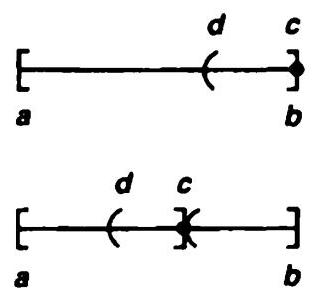
\includegraphics[width=0.2\textwidth]{images/24.1.jpg}
\end{center}
\hspace*{3em} 

Figure 24.1

\begin{center}
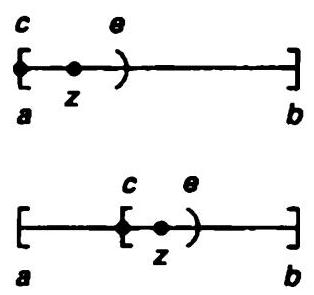
\includegraphics[width=0.2\textwidth]{images/24.2.jpg}
\end{center}
\hspace*{3em} 

Figure 24.2

Case 2. Suppose that \(c \in {A}_{0}\) . Then \(c \neq b\) , so either \(c = a\) or \(a < c < b\) . Because \({A}_{0}\) is open in \(\left\lbrack {a,b}\right\rbrack\) , there must be some interval of the form \(\lbrack c,e)\) contained in \({A}_{0}\) . See Figure 24.2. Because of order property (2) of the linear continuum \(L\) , we can choose a point \(z\) of \(L\) such that \(c < z < e\) . Then \(z \in {A}_{0}\) , contrary to the fact that \(c\) is an upper bound for \({A}_{0}\) .
\end{proof}

\begin{corollary} The real line \(\mathbb{R}\) is connected and so are intervals and rays in \(\mathbb{R}\) .
\end{corollary}

As an application, we prove the intermediate value theorem of calculus, suitably generalized.

\begin{theorem}[Intermediate value theorem] Let \(f: X \rightarrow Y\) be a continuous map, where \(X\) is a connected space and \(Y\) is an ordered set in the order topology. If a and \(b\) are two points of \(X\) and if \(r\) is a point of \(Y\) lying between \(f\left( a\right)\) and \(f\left( b\right)\) , then there exists a point \(c\) of \(X\) such that \(f\left( c\right) = r\) .

The intermediate value theorem of calculus is the special case of this theorem that occurs when we take \(X\) to be a closed interval in \(\mathbb{R}\) and \(Y\) to be \(\mathbb{R}\) .

\end{theorem}
\begin{proof}
Assume the hypotheses of the theorem. The sets

\[
A = f\left( X\right) \cap \left( {-\infty,r}\right) \;\text{ and }\;B = f\left( X\right) \cap \left( {r, + \infty }\right)
\]

are disjoint, and they are nonempty because one contains \(f\left( a\right)\) and the other contains \(f\left( b\right)\) . Each is open in \(f\left( X\right)\) , being the intersection of an open ray in \(Y\) with \(f\left( X\right)\) . If there were no point \(c\) of \(X\) such that \(f\left( c\right) = r\) , then \(f\left( X\right)\) would be the union of the sets \(A\) and \(B\) . Then \(A\) and \(B\) would constitute a separation of \(f\left( X\right)\) , contradicting the fact that the image of a connected space under a continuous map is connected.
\end{proof}

\begin{centeredblock}
\begin{example} One example of a linear continuum different from \(\mathbb{R}\) is the ordered square. We check the least upper bound property. (The second property of a linear continuum is trivial to check.) Let \(A\) be a subset of \(I \times I\) , let \({\pi }_{1}I \times I \rightarrow I\) be projection on the first coordinate; let \(b = \sup {\pi }_{1}\left( A\right)\) . If \(b \in {\pi }_{1}\left( A\right)\) , then \(A\) intersects the subset \(b \times I\) of \(I \times I\) . Because \(b \times I\) has the order type of \(I\) , the set \(A \cap \left( {b \times I}\right)\) will have a least upper bound \(b \times c\) , which will be the least upper bound of \(A\) . See Figure 24.3. If \(b \notin {\pi }_{1}\left( A\right)\) , then \(b \times 0\) is the least upper bound of \(A\) ; no element of the form \({b}^{\prime } \times c\) with \({b}^{\prime } < b\) can be an upper bound for \(A\) , for then \({b}^{\prime }\) would be an upper bound for \({\pi }_{l}\left( A\right)\) .

\begin{center}
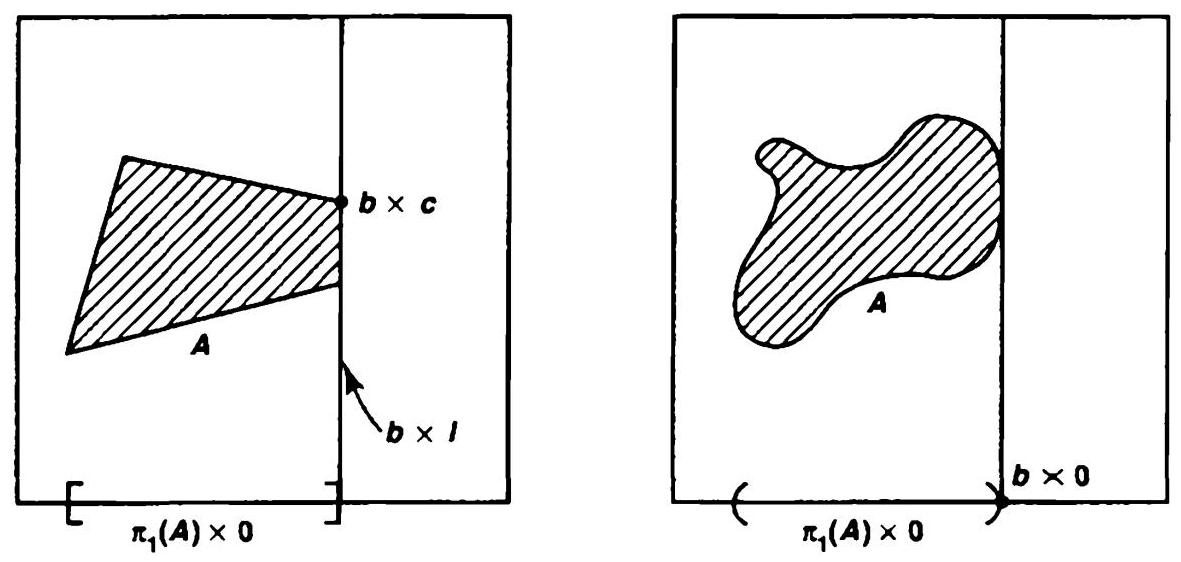
\includegraphics[width=1.0\textwidth]{images/24.3.jpg}
\end{center}
\hspace*{3em}

Figure 24.3
\end{example}
\end{centeredblock}

\begin{centeredblock}
\begin{example} If \(X\) is a well-ordered set, then \(X \times \lbrack 0,1)\) is a linear continuum in the dictionary order; this we leave to you to check. This set can be thought of as having been constructed by ``fitting in'' a set of the order type of(0,1)immediately following each element of \(X\) .
\end{example}
\end{centeredblock}

Connectedness of intervals in \(\mathbb{R}\) gives rise to an especially useful criterion for showing that a space \(X\) is connected; namely, the condition that every pair of points of \(X\) can be joined by a path in \(X\) :

\begin{definition} Given points \(x\) and \(y\) of the space \(X\) , a path in \(X\) from \(x\) to \(y\) is a continuous map \(f: \left\lbrack {a,b}\right\rbrack \rightarrow X\) of some closed interval in the real line into \(X\) , such that \(f\left( a\right) = x\) and \(f\left( b\right) = y\) . A space \(X\) is said to be path connected if every pair of points of \(X\) can be joined by a path in \(X\) .
\end{definition}


It is easy to see that a path-connected space \(X\) is connected. Suppose \(X = A \cup B\) is a separation of \(X\) . Let \(f: \left\lbrack {a,b}\right\rbrack \rightarrow X\) be any path in \(X\) . Being the continuous image of a connected set, the set \(f\left( \left\lbrack {a,b}\right\rbrack \right)\) is connected, so that it lies entirely in either \(A\) or \(B\) . Therefore, there is no path in \(X\) joining a point of \(A\) to a point of \(B\) , contrary to the assumption that \(X\) is path connected.

The converse does not hold; a connected space need not be path connected. See Examples 6 and 7 following.

\begin{centeredblock}
\begin{example} Define the unit ball \({B}^{n}\) in \({\mathbb{R}}^{n}\) by the equation

\[
{B}^{n} = \{ \mathbf{x} \mid \parallel \mathbf{x}\parallel \leq 1\}
\]

where

\[
\parallel \mathbf{x}\parallel = \begin{Vmatrix}\left( {{x}_{1},\ldots,{x}_{n}}\right) \end{Vmatrix} = {\left( {x}_{1}^{2} + \cdots + {x}_{n}^{2}\right) }^{1/2}
\]

The unit ball is path connected; given any two points \(\mathbf{x}\) and \(\mathbf{y}\) of \({B}^{n}\) , the straight-line path \(f: \left\lbrack {0,1}\right\rbrack \rightarrow {\mathbb{R}}^{n}\) defined by

\[
f\left( t\right) = \left( {1 - t}\right) x + {ty}
\]

lies in \({B}^{n}\) . For if \(x\) and \(y\) are in \({B}^{n}\) and \(t\) is in \(\left\lbrack {0,1}\right\rbrack\) ,

\[
\parallel f\left( t\right) \parallel \leq \left( {1 - t}\right) \parallel \mathbf{x}\parallel + t\parallel \mathbf{y}\parallel \leq 1.
\]

A similar argument shows that every open ball \({B}_{d}\left( {\mathbf{x},\epsilon }\right)\) and every closed ball \({\bar{B}}_{d}\left( {\mathbf{x},\epsilon }\right)\) in \({\mathbb{R}}^{n}\) is path connected.
\end{example}
\end{centeredblock}

\begin{centeredblock}
\begin{example} Define punctured euclidean space to be the space \({\mathbb{R}}^{n} - \{ \mathbf{0}\}\) , where0is the origin in \({\mathbb{R}}^{n}\) . If \(n > 1\) , this space is path connected. Given \(\mathbf{x}\) and \(\mathbf{y}\) different from 0, we can join \(x\) and \(y\) by the straight-line path between them if that path does not go through the origin. Otherwise, we can choose a point \(\mathbf{z}\) not on the line joining \(\mathbf{x}\) and \(\mathbf{y}\) , and take the broken-line path from \(x\) to \(z\) , and then from \(z\) to \(y\)
\end{example}
\end{centeredblock}

\begin{centeredblock}
\begin{example} Define the unit sphere \({S}^{n - 1}\) in \({\mathbb{R}}^{n}\) by the equation

\[
{S}^{n - 1} = \{ \mathbf{x} \mid \parallel \mathbf{x}\parallel = 1\} .
\]

If \(n > 1\) , it is path connected. For the map \(g: {\mathbb{R}}^{n} - \{ \mathbf{0}\} \rightarrow {S}^{n - 1}\) defined by \(g\left( \mathbf{x}\right) = \mathbf{x}/\parallel \mathbf{x}\parallel\) is continuous and surjective; and it is easy to show that the continuous image of a path-connected space is path connected.
\end{example}
\end{centeredblock}

\begin{centeredblock}
\begin{example} The ordered square \({I}_{o}^{2}\) is connected but not path connected.

Being a linear continuum, the ordered square is connected. Let \(p = 0 \times 0\) and \(q =\) \(1 \times 1\) . We suppose there is a path \(f: \left\lbrack {a,b}\right\rbrack \rightarrow {I}_{o}^{2}\) joining \(p\) and \(q\) and derive a contradiction. The image set \(f\left( \left\lbrack {a,b}\right\rbrack \right)\) must contain every point \(x \times y\) of \({I}_{o}^{2}\) , by the intermediate value theorem. Therefore, for each \(x \in I\) , the set

\[
{U}_{x} = {f}^{-1}\left( {x \times \left( {0,1}\right) }\right)
\]

is a nonempty subset of \(\left\lbrack {a,b}\right\rbrack\) ; by continuity, it is open in \(\left\lbrack {a,b}\right\rbrack\) . See Figure 24.4. Choose, for each \(x \in I\) , a rational number \({q}_{x}\) beloriging to \({U}_{x}\) . Since the sets \({U}_{x}\) are disjoint, the map \(x \rightarrow {q}_{x}\) is an injective mapping of \(I\) into \(\mathbb{Q}\) . This contradicts the fact that the interval \(I\) is uncountable (which we shall prove later)
\end{example}
\end{centeredblock}

\begin{centeredblock}
\begin{example} Let \(S\) denote the following subset of the plane.

\[
S = \{ x \times \sin \left( {1/x}\right) \mid 0 < x \leq 1\} .
\]

Because \(S\) is the image of the connected set \((0,1\rbrack\) under a continuous map, \(S\) is connected. Therefore, its closure \(\bar{S}\) in \({\mathbb{R}}^{2}\) is also connected. The set \(\bar{S}\) is a classical example in topology called the topologist’s sine curve. It is illustrated in Figure 24.5; it equals the union of \(S\) and the vertical interval \(0 \times \left\lbrack {-1,1}\right\rbrack\) . We show that \(\bar{S}\) is not path connected.

\begin{center}
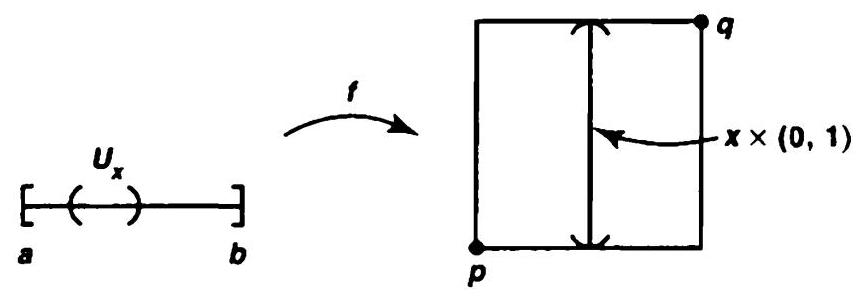
\includegraphics[width=0.7\textwidth]{images/24.4.jpg}
\end{center}
\hspace*{3em} 

Figure 24.4

Suppose there is a path \(f.\left\lbrack {a,c}\right\rbrack \rightarrow \bar{S}\) beginning at the origin and ending at a point of \(S\) . The set of those \(t\) for which \(f\left( t\right) \in 0 \times \left\lbrack {-1,1}\right\rbrack\) is closed, so it has a largest element \(b\) . Then \(f: \left\lbrack {b,c}\right\rbrack \rightarrow \bar{S}\) is a path that maps \(b\) into the vertical interval \(0 \times \left\lbrack {-1,1}\right\rbrack\) and maps the other points of \(\left\lbrack {b,c}\right\rbrack\) to points of \(S\) .

Replace \(\left\lbrack {b,c}\right\rbrack\) by \(\left\lbrack {0,1}\right\rbrack\) for convenience; let \(f\left( t\right) = \left( {x\left( t\right) ,y\left( t\right) }\right)\) . Then \(x\left( 0\right) = 0\) , while \(x\left( t\right) > 0\) and \(y\left( t\right) = \sin \left( {1/x\left( t\right) }\right)\) for \(t > 0\) . We show there is a sequence of points \({t}_{n} \rightarrow 0\) such that \(y\left( {t}_{n}\right) = {\left( -1\right) }^{n}\) . Then the sequence \(y\left( {t}_{n}\right)\) does not converge, contradicting continuity of \(f\) .

To find \({t}_{n}\) , we proceed as follows: Given \(n\) , choose \(u\) with \(0 < u < x\left( {1/n}\right)\) such that \(\sin \left( {1/u}\right) = {\left( -1\right) }^{n}\) . Then use the intermediate value theorem to find \({t}_{n}\) with \(0 < {t}_{n} < 1/n\) such that \(x\left( {t}_{n}\right) = u\) .

\begin{center}
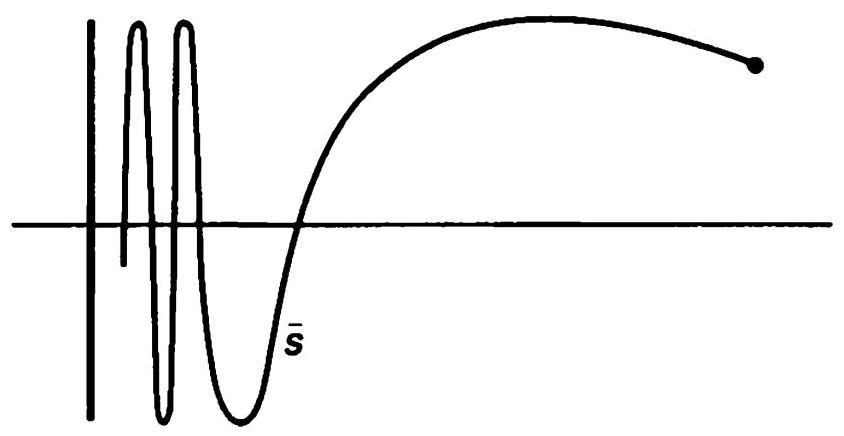
\includegraphics[width=0.7\textwidth]{images/24.5.jpg}
\end{center}
\hspace*{3em} 

Figure 24.5
\end{example}
\end{centeredblock}

\section*{Exercises}

1. (a) Show that no two of the spaces \(\left( {0,1}\right) ,(0,1\rbrack\) , and \(\left\lbrack {0,1}\right\rbrack\) are homeomorphic. [Hint: What happens if you remove a point from each of these spaces?)]

(b) Suppose that there exist imbeddings \(f: X \rightarrow Y\) and \(g: Y \rightarrow X\) . Show by means of an example that \(X\) and \(Y\) need not be homeomorphic.

(c) Show \({\mathbb{R}}^{n}\) and \(\mathbb{R}\) are not homeomorphic if \(n > 1\) .

2. Let \(f: {S}^{1} \rightarrow \mathbb{R}\) be a continuous map. Show there exists a point \(x\) of \({S}^{1}\) such that \(f\left( x\right) = f\left( {-x}\right)\) .

3. Let \(f: X \rightarrow X\) be continuous. Show that if \(X = \left\lbrack {0,1}\right\rbrack\) , there is a point \(x\) such that \(f\left( x\right) = x\) . The point \(x\) is called a fixed point of \(f\) . What happens if \(X\) equals \(\lbrack 0,1)\) or \(\left( {0,1}\right) {}^{7}\)

4. Let \(X\) be an ordered set in the order topology. Show that if \(X\) is connected, then \(X\) is a linear continuum.

5. Consider the following sets in the dictionary order. Which are linear continua?

(a) \({\mathbb{Z}}_{ + } \times \lbrack 0,1)\)

(b) \(\lbrack 0,1) \times {\mathbb{Z}}_{ + }\)

(c) \(\lbrack 0,1) \times \left\lbrack {0,1}\right\rbrack\)

(d) \(\left\lbrack {0,1}\right\rbrack \times \lbrack 0,1)\)

6. Show that if \(X\) is a well-ordered set, then \(X \times \lbrack 0,1)\) in the dictionary order is a linear continuum.

7. (a) Let \(X\) and \(Y\) be ordered sets in the order topology. Show that if \(f: X \rightarrow Y\) is order preserving and surjective, then \(f\) is a homeomorphism.

(b) Let \(X = Y = {\overline{\mathbb{R}}}_{ + }\) . Given a positive integer \(n\) , show that the function \(f\left( x\right) =\) \({x}^{n}\) is order preserving and surjective. Conclude that its inverse, the nth root function, is continuous.

(c) Let \(X\) be the subspace \(\left( {-\infty, - 1}\right) \cup \lbrack 0,\infty )\) of \(\mathbb{R}\) . Show that the function \(f: X \rightarrow \mathbb{R}\) defined by setting \(f\left( x\right) = x + 1\) if \(x < - 1\) , and \(f\left( x\right) = x\) if \(x \geq 0\) , is order preserving and surjective. Is \(f\) a homeomorphism? Compare with (a).

8. (a) Is a product of path-connected spaces necessarily path connected?

(b) If \(A \subset X\) and \(A\) is path connected, is \(\bar{A}\) necessarily path connected?

(c) If \(f: X \rightarrow Y\) is continuous and \(X\) is path connected, is \(f\left( X\right)\) necessarily path connected?

(d) If \(\left\{ {A}_{\alpha }\right\}\) is a collection of path-connected subspaces of \(X\) and if \(\bigcap {A}_{\alpha } \neq \varnothing\) , is \(\bigcup {A}_{\alpha }\) necessarily path connected?

9. Assume that \(\mathbb{R}\) is uncountable. Show that if \(A\) is a countable subset of \({\mathbb{R}}^{2}\) , then \({\mathbb{R}}^{2} - A\) is path connected. [Hint: How many lines are there passing through a given point of \({\mathbb{R}}^{2}\) ?]

10. Show that if \(U\) is an open connected subspace of \({\mathbb{R}}^{2}\) , then \(U\) is path connected. [Hint: Show that given \({x}_{0} \in U\) , the set of points that can be joined to \({x}_{0}\) by a path in \(U\) is both open and closed in \(U\) .]

11. If \(A\) is a connected subspace of \(X\) , does it follow that Int \(A\) and Bd \(A\) are connected? Does the converse hold? Justify your answers.

*12. Recall that \({S}_{\Omega }\) denotes the minimal uncountable well-ordered set. Let \(L\) denote the ordered set \({S}_{\Omega } \times \lbrack 0,1)\) in the dictionary order, with its smallest element deleted. The set \(L\) is a classical example in topology called the long line.

\begin{theorem} The long line is path connected and locally homeomorphic to \(\mathbb{R}\) , but it cannot be imbedded in \(\mathbb{R}\) .

(a) Let \(X\) be an ordered set; let \(a < b < c\) be points of \(X\) . Show that \(\lbrack a,c)\) has the order type of \(\lbrack 0,1)\) if and only if both \(\lbrack a,b)\) and \(\lbrack b,c)\) have the order type of \(\lbrack 0,1)\)

(b) Let \(X\) be an ordered set. Let \({x}_{0} < {x}_{1} < \cdots\) be an increasing sequence of points of \(X\) ; suppose \(b = \sup \left\{ {x}_{t}\right\}\) Show that \(\left\lbrack {{x}_{0},b}\right)\) has the order type of \(\lbrack 0,1)\) if and only if each interval \(\left\lbrack {{x}_{i},{x}_{i + 1}}\right)\) has the order type of \(\lbrack 0,1)\) .

(c) Let \({a}_{0}\) denote the smallest element of \({S}_{\Omega }\) . For each element \(a\) of \({S}_{\Omega }\) different from \({a}_{0}\) , show that the interval \(\left\lbrack {{a}_{0} \times 0,a \times 0}\right)\) of \({S}_{\Omega } \times \lbrack 0,1)\) has the order type of \(\lbrack 0,1)\) . [Hint: Proceed by transfinite induction. Either \(a\) has an immediate predecessor in \({S}_{\Omega }\) , or there is an increasing sequence \({a}_{t}\) in \({S}_{\Omega }\) with \(a = \sup \left\{ {a}_{i}\right\}\) .

(d) Show that \(L\) is path connected.

(e) Show that every point of \(L\) has a neighborhood homeomorphic with an open interval in \(\mathbb{R}\) .

(f) Show that \(L\) cannot be imbedded in \(\mathbb{R}\) , or indeed in \({\mathbb{R}}^{n}\) for any \(n\) . [Hint: Any subspace of \({\mathbb{R}}^{n}\) has a countable basis for its topology.]

\end{theorem}
\section*{*§ 25 Components and Local Connectedness \protect\sectionDagger}

Given an arbitrary space \(X\) , there is a natural way to break it up into pieces that are connected (or path connected). We consider that process now.

\begin{definition} Given \(X\) , define an equivalence relation on \(X\) by setting \(x \sim y\) if there is a connected subspace of \(X\) containing both \(x\) and \(y\) . The equivalence classes are called the components (or the ``connected components'') of \(X\) .
\end{definition}


Symmetry and reflexivity of the relation are obvious. Transitivity follows by noting that if \(A\) is a connected subspace containing \(x\) and \(y\) , and if \(B\) is a connected subspace containing \(y\) and \(z\) , then \(A \cup B\) is a subspace containing \(x\) and \(z\) that is connected because \(A\) and \(B\) have the point \(y\) in common.

The components of \(X\) can also be described as follows:

\begin{theorem} The components of \(X\) are connected disjoint subspaces of \(X\) whose union is \(X\) , such that each nonempty connected subspace of \(X\) intersects only one of them.

\end{theorem}
\begin{proof}
Being equivalence classes, the components of \(X\) are disjoint and their union is \(X\) . Each connected subspace \(A\) of \(X\) intersects only one of them. For if \(A\) intersects the components \({C}_{1}\) and \({C}_{2}\) of \(X\) , say in points \({x}_{1}\) and \({x}_{2}\) , respectively, then \({x}_{1} \sim {x}_{2}\) by definition; this cannot happen unless \({C}_{1} = {C}_{2}\) .

\customfootnote
{
${}^{\dagger}$ This section will be assumed in Part II of the book.
}

To show the component \(C\) is connected, choose a point \({x}_{0}\) of \(C\) . For each point \(x\) of \(C\) , we know that \({x}_{0} \sim x\) , so there is a connected subspace \({A}_{x}\) containing \({x}_{0}\) and \(x\) . By the result just proved, \({A}_{x} \subset C\) . Therefore,

\[
C = \mathop{\bigcup }\limits_{{x \in C}}{A}_{x}
\]

Since the subspaces \({A}_{x}\) are connected and have the point \({x}_{0}\) in common, their union is connected.
\end{proof}

\begin{definition} We define another equivalence relation on the space \(X\) by defining \(x \sim y\) if there is a path in \(X\) from \(x\) to \(y\) . The equivalence classes are called the path components of \(X\) .
\end{definition}


Let us show this is an equivalence relation. First we note that if there exists a path \(f: \left\lbrack {a,b}\right\rbrack \rightarrow X\) from \(x\) to \(y\) whose domain is the interval \(\left\lbrack {a,b}\right\rbrack\) , then there is also a path \(g\) from \(x\) to \(y\) having the closed interval \(\left\lbrack {c,d}\right\rbrack\) as its domain. (This follows from the fact that any two closed intervals in \(\mathbb{R}\) are homeomorphic.) Now the fact that \(x \sim x\) for each \(x\) in \(X\) follows from the existence of the constant path \(f: \left\lbrack {a,b}\right\rbrack \rightarrow X\) defined by the equation \(f\left( t\right) = x\) for all \(t\) . Symmetry follows from the fact that if \(f: \left\lbrack {0,1}\right\rbrack \rightarrow X\) is a path from \(x\) to \(y\) , then the ``reverse path'' \(g: \left\lbrack {0,1}\right\rbrack \rightarrow X\) defined by \(g\left( t\right) = f\left( {1 - t}\right)\) is a path from \(y\) to \(x\) . Finally, transitivity is proved as follows: Let \(f: \left\lbrack {0,1}\right\rbrack \rightarrow X\) be a path from \(x\) to \(y\) , and let \(g.\left\lbrack {1,2}\right\rbrack \rightarrow X\) be a path from \(y\) to \(z\) . We can ``paste \(f\) and \(g\) together'' to get a path \(h: \left\lbrack {0,2}\right\rbrack \rightarrow X\) from \(x\) to \(z\) ; the path \(h\) will be continuous by the ``pasting lemma,'' Theorem 18.3.

One has the following theorem, whose proof is similar to that of the theorem preceding:

\begin{theorem} The path components of \(X\) are path-connected disjoint subspaces of \(X\) whose union is \(X\) , such that each nonempty path-connected subspace of \(X\) intersects only one of them.

Note that each component of a space \(X\) is closed in \(X\) , since the closure of a connected subspace of \(X\) is connected. If \(X\) has only finitely many components, then each component is also open in \(X\) , since its complement is a finite union of closed sets But in general the components of \(X\) need not be open in \(X\) .

One can say even less about the path components of \(X\) , for they need be neither open nor closed in \(X\) . Consider the following examples:

\begin{centeredblock}
\begin{example} If \(\mathbb{Q}\) is the subspace of \(\mathbb{R}\) consisting of the rational numbers, then each component of \(\mathbb{Q}\) consists of a single point. None of the components of \(\mathbb{Q}\) are open in \(\mathbb{Q}\) .
\end{example}
\end{centeredblock}

\begin{centeredblock}
\begin{example} The ``topologist's sine curve'' \(\bar{S}\) of the preceding section is a space that has a single component (since it is connected) and two path components One path component is the curve \(S\) and the other is the vertical interval \(V = 0 \times \left\lbrack {-1,1}\right\rbrack\) . Note that \(S\) is open in \(\bar{S}\) but not closed, while \(V\) is closed but not open

If one forms a space from \(\widetilde{S}\) by deleting all points of \(V\) having rational second coordinate, one obtains a space that has only one component but uncountably many path components.
\end{example}
\end{centeredblock}

Connectedness is a useful property for a space to possess. But for some purposes, it is more important that the space satisfy a connectedness condition locally. Roughly speaking, local connectedness means that each point has ``arbitrarily small'' neighborhoods that are connected. More precisely, one has the following definition:

\begin{definition} A space \(X\) is said to be locally connected at \(x\) if for every neighborhood \(U\) of \(x\) , there is a connected neighborhood \(V\) of \(x\) contained in \(U\) If \(X\) is locally connected at each of its points, it is said simply to be locally connected. Similarly, a space \(X\) is said to be locally path connected at \(x\) if for every neighborhood \(U\) of \(x\) , there is a path-connected neighborhood \(V\) of \(x\) contained in \(U\) . If \(X\) is locally path connected at each of its points, then it is said to be locally path connected.
\end{definition}


\begin{centeredblock}
\begin{example} Each interval and each ray in the real line is both connected and locally connected The subspace \(\left\lbrack {-1,0)\cup (0,1}\right\rbrack\) of \(\mathbb{R}\) is not connected, but it is locally connected The topologist’s sine curve is connected but not locally connected. The rationals \(\mathbb{Q}\) are neither connected nor locally connected.
\end{example}
\end{centeredblock}

\end{theorem}
\begin{theorem} A space \(X\) is locally connected if and only if for every open set \(U\) of \(X\) , each component of \(U\) is open in \(X\) .

\end{theorem}
\begin{proof}
Suppose that \(X\) is locally connected; let \(U\) be an open set in \(X\) ; let \(C\) be a component of \(U\) If \(x\) is a point of \(C\) , we can choose a connected neighborhood \(V\) of \(x\) such that \(V \subset U\) . Since \(V\) is connected, it must lie entirely in the component \(C\) of \(U\) . Therefore, \(C\) is open in \(X\) .

Conversely, suppose that components of open sets in \(X\) are open. Given a point \(x\) of \(X\) and a neighborhood \(U\) of \(x\) , let \(C\) be the component of \(U\) containing \(x\) . Now \(C\) is connected; since it is open in \(X\) by hypothesis, \(X\) is locally connected at \(x\) .

A similar proof holds for the following theorem:

\begin{theorem} A space \(X\) is locally path connected if and only if for every open set \(U\) of \(X\) , each path component of \(U\) is open in \(X\) .

The relation between path components and components is given in the following theorem:

\end{theorem}
\begin{theorem} If \(X\) is a topological space, each path component of \(X\) lies in a component of \(X\) If \(X\) is locally path connected, then the components and the path components of \(X\) are the same.

\({Proof}\) . Let \(C\) be a component of \(X\) ; let \(x\) be a point of \(C\) ; let \(P\) be the path component of \(X\) containing \(x\) . Since \(P\) is connected, \(P \subset C\) . We wish to show that if \(X\) is locally path connected, \(P = C\) . Suppose that \(P \subsetneq C\) . Let \(Q\) denote the union of all the path components of \(X\) that are different from \(P\) and intersect \(C\) , each of them necessarily lies in \(C\) , so that

\[
C = P \cup Q\text{ . }
\]

Because \(X\) is locally path connected, each path component of \(X\) is open in \(X\) . Therefore, \(P\) (which is a path component) and \(Q\) (which is a union of path components) are open in \(X\) , so they constitute a separation of \(C\) . This contradicts the fact that \(C\) is connected.

\end{theorem}
\end{proof}
\section*{Exercises}

1. What are the components and path components of \({\mathbb{R}}_{\ell }\) ? What are the continuous maps \(f: \mathbb{R} \rightarrow {\mathbb{R}}_{\ell }\) ?

2. (a) What are the components and path components of \({\mathbb{R}}^{\omega }\) (in the product topology)?

(b) Consider \({\mathbb{R}}^{\omega }\) in the uniform topology. Show that \(\mathbf{x}\) and \(\mathbf{y}\) lie in the same component of \({\mathbb{R}}^{\omega }\) if and only if the sequence

\[
\mathbf{x} - \mathbf{y} = \left( {{x}_{1} - {y}_{1},{x}_{2} - {y}_{2},\ldots }\right)
\]

is bounded. [Hint: It suffices to consider the case where \(\mathbf{y} = \mathbf{0}\) .]

(c) Give \({\mathbb{R}}^{\omega }\) the box topology. Show that \(\mathbf{x}\) and \(\mathbf{y}\) lie in the same component of \({\mathbb{R}}^{\omega }\) if and only if the sequence \(\mathbf{x} - \mathbf{y}\) is ``eventually zero.'' [Hint: If \(\mathbf{x} - \mathbf{y}\) is not eventually zero, show there is homeomorphism \(h\) of \({\mathbb{R}}^{\omega }\) with itself such that \(h\left( \mathbf{x}\right)\) is bounded and \(h\left( \mathbf{y}\right)\) is unbounded.]

3. Show that the ordered square is locally connected but not locally path connected. What are the path components of this space?

4. Let \(X\) be locally path connected. Show that every connected open set in \(X\) is path connected.

5. Let \(X\) denote the rational points of the interval \(\left\lbrack {0,1}\right\rbrack \times 0\) of \({\mathbb{R}}^{2}\) . Let \(T\) denote the union of all line segments joining the point \(p = 0 \times 1\) to points of \(X\) .

(a) Show that \(T\) is path connected, but is locally connected only at the point \(p\) .

(b) Find a subset of \({\mathbb{R}}^{2}\) that is path connected but is locally connected at none of its points.

6. A space \(X\) is said to be weakly locally connected at \(x\) if for every neighborhood \(U\) of \(x\) , there is a connected subspace of \(X\) contained in \(U\) that contains a neighborhood of \(x\) . Show that if \(X\) is weakly locally connected at each of its points, then \(X\) is locally connected. [Hint: Show that components of open sets are open.]

7. Consider the ``infinite broom'' \(X\) pictured in Figure 25.1. Show that \(X\) is not locally connected at \(p\) , but is weakly locally connected at \(p\) . [Hint: Any connected neighborhood of \(p\) must contain all the points \({a}_{i}\) .]

\begin{center}
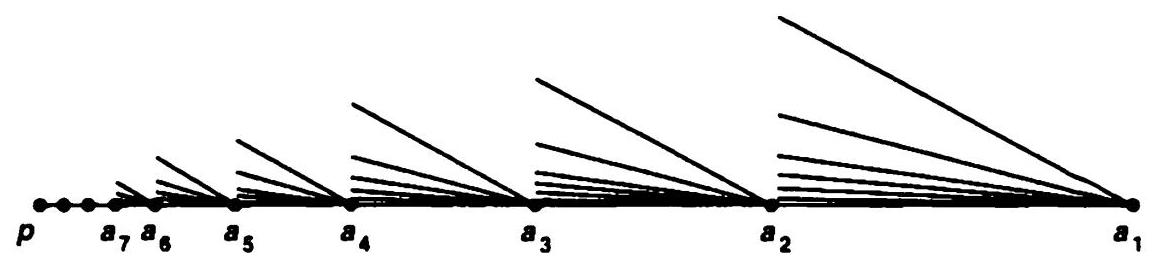
\includegraphics[width=1.0\textwidth]{images/25.1.jpg}
\end{center}
\hspace*{3em} 

Figure 25.1

8. Let \(p: X \rightarrow Y\) be a quotient map. Show that if \(X\) is locally connected, then \(Y\) is locally connected. [Hint: If \(C\) is a component of the open set \(U\) of \(Y\) , show that \({p}^{-1}\left( C\right)\) is a union of components of \({p}^{-1}\left( U\right)\) .]

9. Let \(G\) be a topological group; let \(C\) be the component of \(G\) containing the identity element \(e\) . Show that \(C\) is a normal subgroup of \(G\) . [Hint: If \(x \in G\) , then \({xC}\) is the component of \(G\) containing \(x\) .]

10. Let \(X\) be a space. Let us define \(x \sim y\) if there is no separation \(X = A \cup B\) of \(X\) into disjoint open sets such that \(x \in A\) and \(y \in B\) .

(a) Show this relation is an equivalence relation. The equivalence classes are called the quasicomponents of \(X\) .

(b) Show that each component of \(X\) lies in a quasicomponent of \(X\) , and that the components and quasicomponents of \(X\) are the same if \(X\) is locally connected.

(c) Let \(K\) denote the set \(\left\{ {1/n \mid n \in {\mathbb{Z}}_{ + }}\right\}\) and let \(- K\) denote the set \(\{ - 1/n \mid n \in\) \(\left. {\mathbb{Z}}_{ + }\right\}\) . Determine the components, path components, and quasicomponents of the following subspaces of \({\mathbb{R}}^{2}\) :

\[
A = \left( {K \times \left\lbrack {0,1}\right\rbrack }\right) \cup \{ 0 \times 0\} \cup \{ 0 \times 1\} .
\]

\[
B = A \cup \left( {\left\lbrack {0,1}\right\rbrack \times \{ 0\rbrack }\right) \text{ . }
\]

\[
C = \left( {K \times \left\lbrack {0,1}\right\rbrack }\right) \cup \left( {-K \times \left\lbrack {-1,0}\right\rbrack }\right) \cup \left( {\left\lbrack {0,1}\right\rbrack \times - K}\right) \cup \left( {\left\lbrack {-1,0}\right\rbrack \times K}\right) .
\]

\section*{§ 26 Compact Spaces}

The notion of compactness is not nearly so natural as that of connectedness. From the beginnings of topology, it was clear that the closed interval \(\left\lbrack {a,b}\right\rbrack\) of the real line had a certain property that was crucial for proving such theorems as the maximum value theorem and the uniform continuity theorem. But for a long time, it was not clear how this property should be formulated for an arbitrary topological space It used to be thought that the crucial property of \(\left\lbrack {a,b}\right\rbrack\) was the fact that every infinite subset of \(\left\lbrack {a,b}\right\rbrack\) has a limit point, and this property was the one dignified with the name of compactness. Later, mathematicians realized that this formulation does not lie at the heart of the matter, but rather that a stronger formulation, in terms of open coverings of the space, is more central. The latter formulation is what we now call compactness. It is not as natural or intuitive as the former; some familiarity with it is needed before its usefulness becomes apparent.

\begin{definition} A collection \(\mathcal{A}\) of subsets of a space \(X\) is said to cover \(X\) , or to be a covering of \(X\) , if the union of the elements of \(\mathcal{A}\) is equal to \(X\) . It is called an open covering of \(X\) if its elements are open subsets of \(X\) .
\end{definition}


\begin{definition} A space \(X\) is said to be compact if every open covering \(\mathcal{A}\) of \(X\) contains a finite subcollection that also covers \(X\) .
\end{definition}


\begin{centeredblock}
\begin{example} The real line \(\mathbb{R}\) is not compact, for the covering of \(\mathbb{R}\) by open intervals

\[
\mathcal{A} = \{ \left( {n,n + 2}\right) \mid n \in \mathbb{Z}\}
\]

contains no finite subcollection that covers \(\mathbb{R}\) .
\end{example}
\end{centeredblock}

\begin{centeredblock}
\begin{example} The following subspace of \(\mathbb{R}\) is compact:

\[
X = \{ 0\} \cup \{ 1/n \mid n \in {\mathbb{Z}}_{ + }\} .
\]

Given an open covering \(\mathcal{A}\) of \(X\) , there is an element \(U\) of \(\mathcal{A}\) containing 0. The set \(U\) contains all but finitely many of the points \(1/n\) ; choose, for each point of \(X\) not in \(U\) , an element of \(\mathcal{A}\) containing it. The collection consisting of these elements of \(\mathcal{A}\) , along with the element \(U\) , is a finite subcollection of \(\mathcal{A}\) that covers \(X\) .
\end{example}
\end{centeredblock}

\begin{centeredblock}
\begin{example} Any space \(X\) containing only finitely many points is necessarily compact, because in this case every open covering of \(X\) is finite.
\end{example}
\end{centeredblock}

\begin{centeredblock}
\begin{example} The interval \((0,1\rbrack\) is not compact; the open covering

\[
\mathcal{A} = \left\{ {(l/n,1\rbrack \mid n \in {\mathbb{Z}}_{ + }}\right\}
\]

contains no finite subcollection covering \((0,1\}\) . Nor is the interval(0,1)compact; the same argument applies. On the other hand, the interval \(\left\lbrack {0,1}\right\rbrack\) is compact; you are probably already famuliar with this fact from analysis. In any case, we shall prove it shortly.
\end{example}
\end{centeredblock}

In general, it takes some effort to decide whether a given space is compact or not. First we shall prove some general theorems that show us how to construct new compact spaces out of existing ones. Then in the next section we shall show certain specific spaces are compact. These spaces include all closed intervals in the real line, and all closed and bounded subsets of \({\mathbb{R}}^{n}\) .

Let us first prove some facts about subspaces. If \(Y\) is a subspace of \(X\) , a collection \(\mathcal{A}\) of subsets of \(X\) is said to cover \(Y\) if the union of its elements contains \(Y\) .

\begin{lemma} Let \(Y\) be a subspace of \(X\) . Then \(Y\) is compact if and only if every covering of \(Y\) by sets open in \(X\) contains a finite subcollection covering \(Y\) .
\end{lemma}

\begin{proof}
Suppose that \(Y\) is compact and \(\mathcal{A} = {\left\{ {A}_{\alpha }\right\} }_{\alpha \in J}\) is a covering of \(Y\) by sets open in \(X\) . Then the collection

\[
\left\{ {{A}_{\alpha } \cap Y \mid \alpha \in J}\right\}
\]

is a covering of \(Y\) by sets open in \(Y\) ; hence a finite subcollection

\[
\left\{ {{A}_{{\alpha }_{1}} \cap Y,\ldots,{A}_{{\alpha }_{n}} \cap Y}\right\}
\]

covers \(Y\) . Then \(\left\{ {{A}_{{\alpha }_{1}},\ldots,{A}_{{\alpha }_{n}}}\right\}\) is a subcollection of \(\mathcal{A}\) that covers \(Y\) .

Conversely, suppose the given condition holds; we wish to prove \(Y\) compact. Let \({\mathcal{A}}^{\prime } = \left\{ {A}_{\alpha }^{\prime }\right\}\) be a covering of \(Y\) by sets open in \(Y\) . For each \(\alpha\) , choose a set \({A}_{\alpha }\) open in \(X\) such that

\[
{A}_{\alpha }^{\prime } = {A}_{\alpha } \cap Y
\]

The collection \(\mathcal{A} = \left\{ {A}_{\alpha }\right\}\) is a covering of \(Y\) by sets open in \(X\) By hypothesis, some finite subcollection \(\left\{ {{A}_{{\alpha }_{1}},\ldots,{A}_{{\alpha }_{n}}}\right\}\) covers \(Y\) . Then \(\left\{ {{A}_{{\alpha }_{1}}^{\prime },\ldots,{A}_{{\alpha }_{n}}^{\prime }}\right\}\) is a subcollection of \({\mathcal{A}}^{\prime }\) that covers \(Y\)
\end{proof}

\section*{Theorem 26.2. Every closed subspace of a compact space is compact.}

\begin{proof}
Let \(Y\) be a closed subspace of the compact space \(X\) . Given a covering \(\mathcal{A}\) of \(Y\) by sets open in \(X\) , let us form an open covering \(\mathcal{B}\) of \(X\) by adjoining to \(\mathcal{A}\) the single open set \(X - Y\) , that is,

\[
\mathcal{B} = \mathcal{A} \cup \{ X - Y\} .
\]

Some finite subcollection of \(\mathcal{B}\) covers \(X\) . If this subcollection contains the set \(X - Y\) , discard \(X - Y\) ; otherwise, leave the subcollection alone. The resulting collection is a finite subcollection of \(\mathcal{A}\) that covers \(Y\) .
\end{proof}

\section*{Theorem 26.3. Every compact subspace of a Hausdorff space is closed.}

\begin{proof}
Let \(Y\) be a compact subspace of the Hausdorff space \(X\) . We shall prove that \(X - Y\) is open, so that \(Y\) is closed.

Let \({x}_{0}\) be a point of \(X - Y\) . We show there is a neighborhood of \({x}_{0}\) that is disjoint from \(Y\) . For each point \(y\) of \(Y\) , let us choose disjoint neighborhoods \({U}_{y}\) and \({V}_{y}\) of the points \({x}_{0}\) and \(y\) , respectively (using the Hausdorff condition). The collection \(\left\{ {{V}_{y} \mid y \in }\right.\) \(Y\}\) is a covering of \(Y\) by sets open in \(X\) ; therefore, finitely many of them \({V}_{{y}_{1}},\ldots,{V}_{{y}_{n}}\) cover \(Y\) . The open set

\[
V = {V}_{{y}_{1}} \cup \cdot \cup {V}_{{y}_{n}}
\]

contains \(Y\) , and it is disjoint from the open set

\[
U = {U}_{{y}_{1}} \cap \cdots \cap {U}_{{y}_{n}}
\]

formed by taking the intersection of the corresponding neighborhoods of \({x}_{0}\) . For if \(z\) is a point of \(V\) , then \(z \in {V}_{{y}_{i}}\) for some \(i\) , hence \(z \notin {U}_{{y}_{i}}\) and so \(z \notin U\) . See Figure 26.1.

Then \(U\) is a neighborhood of \({x}_{0}\) disjoint from \(Y\) , as desired.

\begin{center}
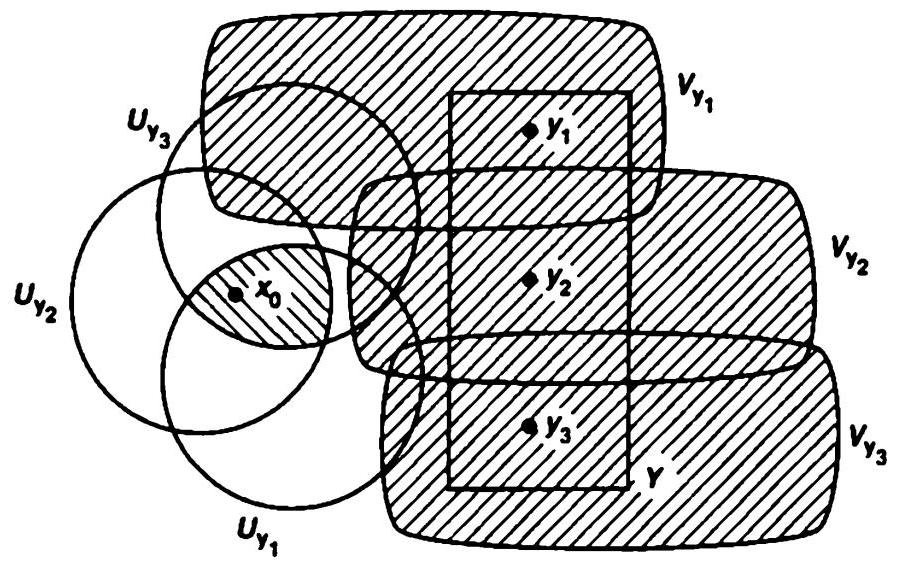
\includegraphics[width=0.8\textwidth]{images/26.1.jpg}
\end{center}
\hspace*{3em} 

Figure 26.1

The statement we proved in the course of the preceding proof will be useful to us later, so we repeat it here for reference purposes:
\end{proof}

\begin{lemma} If \(Y\) is a compact subspace of the Hausdorff space \(X\) and \({x}_{0}\) is not in \(Y\) , then there exist disjoint open sets \(U\) and \(V\) of \(X\) containing \({x}_{0}\) and \(Y\) , respectively.
\end{lemma}

\begin{centeredblock}
\begin{example} Once we prove that the interval \(\left\lbrack {a,b}\right\rbrack\) in \(\mathbb{R}\) is compact, it follows from Theorem 26 2 that any closed subspace of \(\left\lbrack {a,b}\right\rbrack\) is compact. On the other hand, it follows from Theorem 26.3 that the intervals \((a,b\rbrack\) and(a, b)in \(\mathbb{R}\) cannot be compact (which we knew already) because they are not closed in the Hausdorff space \(\mathbf{R}\)
\end{example}
\end{centeredblock}

\begin{centeredblock}
\begin{example} One needs the Hausdorff condition in the hypothesis of Theorem 263 Consider, for example, the finite complement topology on the real line The only proper subsets of \(\mathbb{R}\) that are closed in this topology are the finite sets. But every subset of \(\mathbb{R}\) is compact in this topology, as you can check.
\end{example}
\end{centeredblock}

\begin{theorem} The image of a compact space under a continuous map is compact.

\end{theorem}
\begin{proof}
Let \(f: X \rightarrow Y\) be continuous; let \(X\) be compact. Let \(\mathcal{A}\) be a covering of the set \(f\left( X\right)\) by sets open in \(Y\) . The collection

\[
\left\{ {{f}^{-1}\left( A\right) \mid A \in \mathcal{A}}\right\}
\]

is a collection of sets covering \(X\) ; these sets are open in \(X\) because \(f\) is continuous. Hence finitely many of them, say

\[
{f}^{-1}\left( {A}_{1}\right) ,\ldots,{f}^{-1}\left( {A}_{n}\right) ,
\]

cover \(X\) . Then the sets \({A}_{1},\ldots,{A}_{n}\) cover \(f\left( X\right)\) .

One important use of the preceding theorem is as a tool for verifying that a map is a homeomorphism:

\begin{theorem} Let \(f: X \rightarrow Y\) be a bijective continuous function If \(X\) is compact and \(Y\) is Hausdorff, then \(f\) is a homeomorphism

\end{theorem}
Proof. We shall prove that images of closed sets of \(X\) under \(f\) are closed in \(Y\) ; this will prove continuity of the map \({f}^{-1}\) . If \(A\) is closed in \(X\) , then \(A\) is compact, by Theorem 26.2. Therefore, by the theorem just proved, \(f\left( A\right)\) is compact. Since \(Y\) is Hausdorff, \(f\left( A\right)\) is closed in \(Y\) , by Theorem 26.3.

\begin{theorem} The product of finitely many compact spaces is compact.

\end{theorem}
Proof. We shall prove that the product of two compact spaces is compact; the theorem follows by induction for any finite product.

Step 1. Suppose that we are given spaces \(X\) and \(Y\) , with \(Y\) compact. Suppose that \({x}_{0}\) is a point of \(X\) , and \(N\) is an open set of \(X \times Y\) containing the ``slice'' \({x}_{0} \times Y\) of \(X \times Y\) We prove the following

There is a neighborhood \(W\) of \({x}_{0}\) in \(X\) such that \(N\) contains the entire set \(W \times Y\)

The set \(W \times Y\) is often called a tube about \({x}_{0} \times Y\) .

First let us cover \({x}_{0} \times Y\) by basis elements \(U \times V\) (for the topology of \(X \times Y\) ) lying in \(N\) . The space \({x}_{0} \times Y\) is compact, being homeomorphic to \(Y\) . Therefore, we can cover \({x}_{0} \times Y\) by finitely many such basis elements

\[
{U}_{1} \times {V}_{1},\ldots,{U}_{n} \times {V}_{n}
\]

(We assume that each of the basis elements \({U}_{i} \times {V}_{i}\) actually intersects \({x}_{0} \times Y\) , since otherwise that basis element would be superfluous; we could discard it from the finite collection and still have a covering of \({x}_{0} \times Y\) .) Define

\[
W = {U}_{1} \cap \cdots \cap {U}_{n}
\]

The set \(W\) is open, and it contains \({x}_{0}\) because each set \({U}_{i} \times {V}_{i}\) intersects \({x}_{0} \times Y\) .

We assert that the sets \({U}_{i} \times {V}_{i}\) , which were chosen to cover the slice \({x}_{0} \times Y\) , actually cover the tube \(W \times Y\) . Let \(x \times y\) be a point of \(W \times Y\) . Consider the point \({x}_{0} \times y\) of the slice \({x}_{0} \times Y\) having the same \(y\) -coordinate as this point. Now \({x}_{0} \times y\) belongs to \({U}_{i} \times {V}_{i}\) for some \(i\) , so that \(y \in {V}_{i}\) . But \(x \in {U}_{j}\) for every \(j\) (because \(x \in W\) ). Therefore, we have \(x \times y \in {U}_{i} \times {V}_{i}\) , as desired.

Since all the sets \({U}_{i} \times {V}_{i}\) lie in \(N\) , and since they cover \(W \times Y\) , the tube \(W \times Y\) lies in \(N\) also. See Figure 26.2.

Step 2. Now we prove the theorem. Let \(X\) and \(Y\) be compact spaces. Let \(\mathcal{A}\) be an open covering of \(X \times Y\) . Given \({x}_{0} \in X\) , the slice \({x}_{0} \times Y\) is compact and may therefore be covered by finitely many elements \({A}_{1},\ldots,{A}_{m}\) of \(\mathcal{A}\) . Their union \(N = {A}_{1} \cup \cdots \cup {A}_{m}\) is an open set containing \({x}_{0} \times Y\) ; by Step 1, the open set \(N\) contains a tube \(W \times Y\) about \({x}_{0} \times Y\) , where \(W\) is open in \(X\) . Then \(W \times Y\) is covered by finitely many elements \({A}_{1},\ldots,{A}_{m}\) of \(\mathcal{A}\) .

\begin{center}
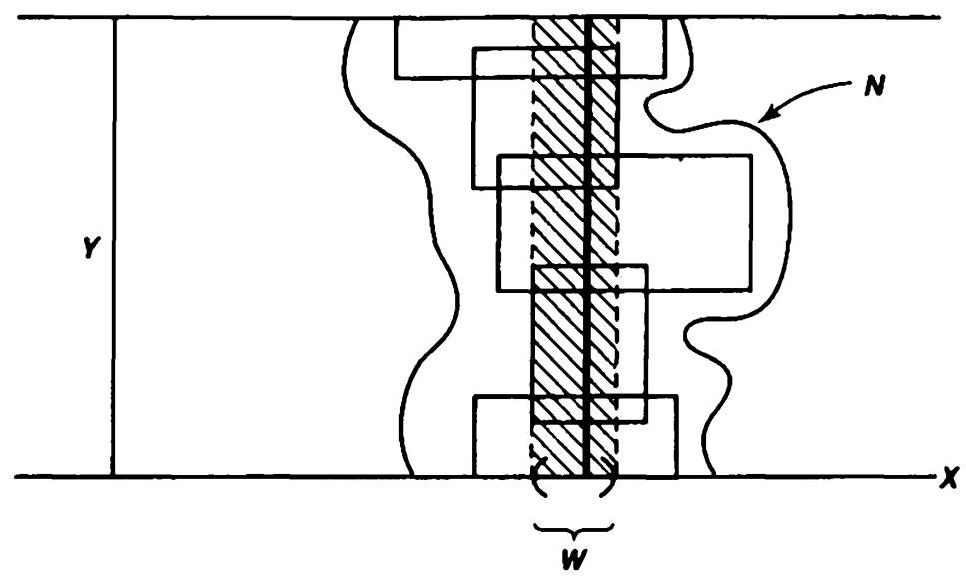
\includegraphics[width=0.8\textwidth]{images/26.2.jpg}
\end{center}
\hspace*{3em} 

Figure 26.2

Thus, for each \(x\) in \(X\) , we can choose a neighborhood \({W}_{x}\) of \(x\) such that the tube \({W}_{x} \times Y\) can be covered by finitely many elements of \(\mathcal{A}\) . The collection of all the neighborhoods \({W}_{x}\) is an open covering of \(X\) ; therefore by compactness of \(X\) , there exists a finite subcollection

\[
\left\{ {{W}_{1},\ldots,{W}_{k}}\right\}
\]

covering \(X\) . The union of the tubes

\[
{W}_{1} \times Y,\ldots,{W}_{k} \times Y
\]

is all of \(X \times Y\) ; since each may be covered by finitely many elements of \(\mathcal{A}\) , so may \(X \times Y\) be covered.

The statement proved in Step 1 of the preceding proof will be useful to us later, so we repeat it here as a lemma, for reference purposes:
\end{proof}

\begin{lemma}[The tube lemma] Consider the product space \(X \times Y\) , where \(Y\) is compact. If \(N\) is an open set of \(X \times Y\) containing the slice \({x}_{0} \times Y\) of \(X \times Y\) , then \(N\) contains some tube \(W \times Y\) about \({x}_{0} \times Y\) , where \(W\) is a neighborhood of \({x}_{0}\) in \(X\) .
\end{lemma}

\begin{centeredblock}
\begin{example} The tube lemma is certainly not true if \(Y\) is not compact For example, let \(Y\) be the \(y\) -axis in \({\mathbb{R}}^{2}\) , and let

\[
N = \left\{ {x \times y,\left| x\right| < 1/\left( {{y}^{2} + 1}\right) }\right\} .
\]

Then \(N\) is an open set containing the set \(0 \times \mathbb{R}\) , but it contains no tube about \(0 \times \mathbb{R}\) It is illustrated in Figure 263

\begin{center}
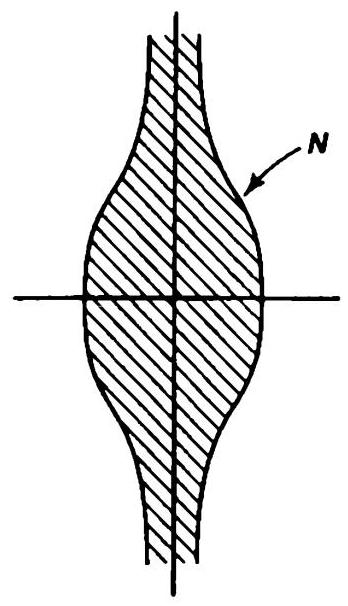
\includegraphics[width=0.3\textwidth]{images/26.3.jpg}
\end{center}
\hspace*{3em}

Figure 26.3
\end{example}
\end{centeredblock}

There is an obvious question to ask at this point. Is the product of infinitely many compact spaces compact? One would hope that the answer is ``yes,'' and in fact it is. The result is important (and difficult) enough to be called by the name of the man who proved it; it is called the Tychonoff theorem

In proving the fact that a cartesian product of connected spaces is connected, one proves it first for finite products and derives the general case from that. In proving that cartesian products of compact spaces are compact, however, there is no way to go directly from finite products to infinite ones. The infinite case demands a new approach, and the proof is a difficult one. Because of its difficulty, and also to avoid losing the main thread of our discussion in this chapter, we have decided to postpone it until later. However, you can study it now if you wish; the section in which it is proved (§37) can be studied immediately after this section without causing any disruption in continuity.

There is one final criterion for a space to be compact, a criterion that is formulated in terms of closed sets rather than open sets It does not look very natural nor very useful at first glance, but it in fact proves to be useful on a number of occasions. First we make a definition.

\begin{definition} A collection \(\mathcal{C}\) of subsets of \(X\) is said to have the finite intersection property if for every finite subcollection

\[
\left\{ {{C}_{1},\ldots,{C}_{n}}\right\}
\]

of \(\mathcal{C}\) , the intersection \({C}_{1} \cap \cdots \cap {C}_{n}\) is nonempty.
\end{definition}

\begin{theorem} Let \(X\) be a topological space. Then \(X\) is compact if and only if for every collection \(\mathcal{C}\) of closed sets in \(X\) having the finite intersection property, the intersection \(\mathop{\bigcap }\limits_{{C \in \mathcal{C}}}C\) of all the elements of \(\mathcal{C}\) is nonempty.
\end{theorem}
\begin{proof}Given a collection \(\mathcal{A}\) of subsets of \(X\) , let

\[
\mathcal{C} = \{ X - A \mid A \in \mathcal{A}\}
\]

be the collection of their complements. Then the following statements hold:

(I) \(\mathcal{A}\) is a collection of open sets if and only if \(\mathcal{C}\) is a collection of closed sets.

(2) The collection \(\mathcal{A}\) covers \(X\) if and only if the intersection \(\mathop{\bigcap }\limits_{{C \in \mathcal{C}}}C\) of all the elements of \(C\) is empty

(3) The finite subcollection \(\left\{ {{A}_{1},\ldots,{A}_{n}}\right\}\) of \(\mathcal{A}\) covers \(X\) if and only if the intersection of the corresponding elements \({C}_{l} = X - {A}_{i}\) of \(\mathcal{C}\) is empty.

The first statement is trivial, while the second and third follow from DeMorgan's law:

\[
X - \left( {\mathop{\bigcup }\limits_{{\alpha \in J}}{A}_{\alpha }}\right) = \mathop{\bigcap }\limits_{{\alpha \in J}}\left( {X - {A}_{\alpha }}\right)
\]

The proof of the theorem now proceeds in two easy steps: taking the contrapositive (of the theorem), and then the complement (of the sets)!

The statement that \(X\) is compact is equivalent to saying: ``Given any collection \(\mathcal{A}\) of open subsets of \(X\) , if \(\mathcal{A}\) covers \(X\) , then some finite subcollection of \(\mathcal{A}\) covers \(X\) .'' This statement is equivalent to its contrapositive, which is the following: ``Given any collection \(\mathcal{A}\) of open sets, if no finite subcollection of \(\mathcal{A}\) covers \(X\) , then \(\mathcal{A}\) does not cover \(X\) .'' Letting \(\mathcal{C}\) be, as earlier, the collection \(\{ X - A \mid A \in \mathcal{A}\}\) and applying (1)-(3), we see that this statement is in turn equivalent to the following: ``Given any collection \(\mathcal{C}\) of closed sets, if every finite intersection of elements of \(\mathcal{C}\) is nonempty, then the intersection of all the elements of \(\mathcal{C}\) is nonempty.'' This is just the condition of our theorem.

A special case of this theorem occurs when we have a nested sequence \({C}_{1} \supset {C}_{2} \supset\) \(\cdots \supset {C}_{n} \supset {C}_{n + 1} \supset \ldots\) of closed sets in a compact space \(X\) . If each of the sets \({C}_{n}\) is nonempty, then the collection \(\mathcal{C} = {\left\{ {C}_{n}\right\} }_{n \in {\mathbf{Z}}_{ + }}\) automatically has the finite intersection property. Then the intersection

\[
\mathop{\bigcap }\limits_{{n \in {\mathbf{Z}}_{ + }}}{C}_{n}
\]

is nonempty.

We shall use the closed set criterion for compactness in the next section to prove the uncountability of the set of real numbers, in Chapter 5 when we prove the Ty-chonoff theorem, and again in Chapter 8 when we prove the Baire category theorem.

\end{proof}
\section*{Exercises}

1. (a) Let \(\mathcal{T}\) and \({\mathcal{T}}^{\prime }\) be two topologies on the set \(X\) ; suppose that \({\mathcal{T}}^{\prime } \supset \mathcal{T}\) . What does compactness of \(X\) under one of these topologies imply about compactness under the other?

(b) Show that if \(X\) is compact Hausdorff under both \(\mathcal{T}\) and \({\mathcal{T}}^{\prime }\) , then either \(\mathcal{T}\) and \({\mathcal{T}}^{\prime }\) are equal or they are not comparable.

2. (a) Show that in the finite complement topology on \(\mathbb{R}\) , every subspace is compact.

(b) If \(\mathbb{R}\) has the topology consisting of all sets \(A\) such that \(\mathbb{R} - A\) is either countable or all of \(\mathbb{R}\) , is \(\left\lbrack {0,1}\right\rbrack\) a compact subspace?

3. Show that a finite union of compact subspaces of \(X\) is compact.

4. Show that every compact subspace of a metric space is bounded in that metric and is closed. Find a metric space in which not every closed bounded subspace is compact.

5. Let \(A\) and \(B\) be disjoint compact subspaces of the Hausdorff space \(X\) . Show that there exist disjoint open sets \(U\) and \(V\) containing \(A\) and \(B\) , respectively.

6. Show that if \(f: X \rightarrow Y\) is continuous, where \(X\) is compact and \(Y\) is Hausdorff, then \(f\) is a closed map (that is, \(f\) carries closed sets to closed sets).

7. Show that if \(Y\) is compact, then the projection \({\pi }_{1} : X \times Y \rightarrow X\) is a closed map.

8. Theorem. Let \(f: X \rightarrow Y\) ; let \(Y\) be compact Hausdorff. Then \(f\) is continuous if and only if the graph of \(f\) ,

\[
{G}_{f} = \{ x \times f\left( x\right) \mid x \in X\}
\]

is closed in \(X \times Y\) . [Hint: If \({G}_{f}\) is closed and \(V\) is a neighborhood of \(f\left( {x}_{0}\right)\) , then the intersection of \({G}_{f}\) and \(X \times \left( {Y - V}\right)\) is closed. Apply Exercise 7.]

9. Generalize the tube lemma as follows:

\begin{theorem} Let \(A\) and \(B\) be subspaces of \(X\) and \(Y\) , respectively; let \(N\) be an open set in \(X \times Y\) containing \(A \times B\) . If \(A\) and \(B\) are compact, then there exist open sets \(U\) and \(V\) in \(X\) and \(Y\) , respectively, such that

\[
A \times B \subset U \times V \subset N.
\]

10. (a) Prove the following partial converse to the uniform limit theorem:

\end{theorem}
\begin{theorem} Let \({f}_{n} : X \rightarrow \mathbb{R}\) be a sequence of continuous functions, with \({f}_{n}\left( x\right) \rightarrow f\left( x\right)\) for each \(x \in X\) . If \(f\) is continuous, and if the sequence \({f}_{n}\) is monotone increasing, and if \(X\) is compact, then the convergence is uniform. [We say that \({f}_{n}\) is monotone increasing if \({f}_{n}\left( x\right) \leq {f}_{n + 1}\left( x\right)\) for all \(n\) and \(x\) .]

(b) Give examples to show that this theorem fails if you delete the requirement that \(X\) be compact, or if you delete the requirement that the sequence be monotone. [Hint: See the exercises of §21.]

11. Theorem. Let \(X\) be a compact Hausdorff space. Let \(\mathcal{A}\) be a collection of closed connected subsets of \(X\) that is simply ordered by proper inclusion. Then

\[
Y = \mathop{\bigcap }\limits_{{A \in \mathcal{A}}}A
\]

is connected. [Hint: If \(C \cup D\) is a separation of \(Y\) , choose disjoint open sets \(U\) and \(V\) of \(X\) containing \(C\) and \(D\) , respectively, and show that

\[
\mathop{\bigcap }\limits_{{A \in \mathcal{A}}}\left( {A - \left( {U \cup V}\right) }\right)
\]

is not empty.]

12. Let \(p: X \rightarrow Y\) be a closed continuous surjective map such that \({p}^{-1}\left( {\{ y\} }\right)\) is compact, for each \(y \in Y\) . (Such a map is called a perfect map ) Show that if \(Y\) is compact, then \(X\) is compact. [Hint: If \(U\) is an open set containing \({p}^{-1}\left( {\{ y\} }\right)\) , there is a neighborhood \(W\) of \(y\) such that \({p}^{-1}\left( W\right)\) is contained in \(U\) ]

13. Let \(G\) be a topological group.

(a) Let \(A\) and \(B\) be subspaces of \(G\) . If \(A\) is closed and \(B\) is compact, show \(A \cdot B\) is closed. [Hint: If \(c\) is not in \(A \cdot B\) , find a neighborhood \(W\) of \(c\) such that \(W \cdot {B}^{-1}\) is disjoint from \(A\) .]

(b) Let \(H\) be a subgroup of \(G\) ; let \(p \cdot G \rightarrow G/H\) be the quotient map. If \(H\) is compact, show that \(p\) is a closed map.

(c) Let \(H\) be a compact subgroup of \(G\) . Show that if \(G/H\) is compact, then \(G\) is compact.

\end{theorem}
\section*{§ 27 Compact Subspaces of the Real Line}

The theorems of the preceding section enable us to construct new compact spaces from existing ones, but in order to get very far we have to find some compact spaces to start with. The natural place to begin is the real line; we shall prove that every closed interval in \(\mathbb{R}\) is compact. Applications include the extreme value theorem and the uniform continuity theorem of calculus, suitably generalized. We also give a characterization of all compact subspaces of \({\mathbb{R}}^{n}\) , and a proof of the uncountability of the set of real numbers.

It turns out that in order to prove every closed interval in \(\mathbb{R}\) is compact, we need only one of the order properties of the real line-the least upper bound property. We shall prove the theorem using only this hypothesis; then it will apply not only to the real line, but to well-ordered sets and other ordered sets as well.

\begin{theorem} Let \(X\) be a simply ordered set having the least upper bound property. In the order topology, each closed interval in \(X\) is compact.

\end{theorem}
\begin{proof}
Step 1. Given \(a < b\) , let \(\mathcal{A}\) be a covering of \(\left\lbrack {a,b}\right\rbrack\) by sets open in \(\left\lbrack {a,b}\right\rbrack\) in the subspace topology (which is the same as the order topology). We wish to prove the existence of a finite subcollection of \(\mathcal{A}\) covering \(\left\lbrack {a,b}\right\rbrack\) . First we prove the following: If \(x\) is a point of \(\left\lbrack {a,b}\right\rbrack\) different from \(b\) , then there is a point \(y > x\) of \(\left\lbrack {a,b}\right\rbrack\) such that the interval \(\left\lbrack {x,y}\right\rbrack\) can be covered by at most two elements of \(\mathcal{A}\)

If \(x\) has an immediate successor in \(X\) , let \(y\) be this immediate successor. Then \(\left\lbrack {x,y}\right\rbrack\) consists of the two points \(x\) and \(y\) , so that it can be covered by at most two elements of \(\mathcal{A}\) . If \(x\) has no immediate successor in \(X\) , choose an element \(A\) of \(\mathcal{A}\) containing \(x\) . Because \(x \neq b\) and \(A\) is open, \(A\) contains an interval of the form \(\lbrack x,c)\) , for some \(c\) in \(\left\lbrack {a,b}\right\rbrack\) . Choose a point \(y\) in(x, c); then the interval \(\left\lbrack {x,y}\right\rbrack\) is covered by the single element \(A\) of \(\mathcal{A}\) .

Step 2. Let \(C\) be the set of all points \(y > a\) of \(\left\lbrack {a,b}\right\rbrack\) such that the interval \(\left\lbrack {a,y}\right\rbrack\) can be covered by finitely many elements of \(\mathcal{A}\) Applying Step 1 to the case \(x = a\) , we see that there exists at least one such \(y\) , so \(C\) is not empty. Let \(c\) be the least upper bound of the set \(C\) ; then \(a < c \leq b\) .

Step 3. We show that \(c\) belongs to \(C\) ; that is, we show that the interval \(\left\lbrack {a,c}\right\rbrack\) can be covered by finitely many elements of \(\mathcal{A}\) . Choose an element \(A\) of \(\mathcal{A}\) containing \(c\) ; since \(A\) is open, it contains an interval of the form \((d,c\rbrack\) for some \(d\) in \(\left\lbrack {a,b}\right\rbrack\) . If \(c\) is not in \(C\) , there must be a point \(z\) of \(C\) lying in the interval(d, c), because otherwise \(d\) would be a smaller upper bound on \(C\) than \(c\) . See Figure 27.1. Since \(z\) is in \(C\) , the interval \(\left\lbrack {a,z}\right\rbrack\) can be covered by finitely many, say \(n\) , elements of \(\mathcal{A}\) . Now \(\left\lbrack {z,c}\right\rbrack\) lies in the single element \(A\) of \(\mathcal{A}\) , hence \(\left\lbrack {a,c}\right\rbrack = \left\lbrack {a,z}\right\rbrack \cup \left\lbrack {z,c}\right\rbrack\) can be covered by \(n + 1\) elements of \(\mathcal{A}\) . Thus \(c\) is in \(C\) , contrary to assumption.

\begin{center}
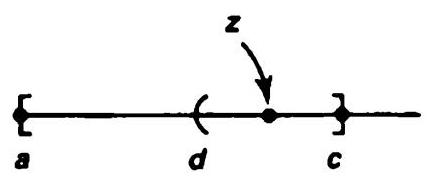
\includegraphics[width=0.4\textwidth]{images/27.1.jpg}
\end{center}
\hspace*{3em} 

Figure 27.1

\begin{center}
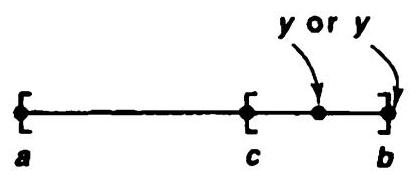
\includegraphics[width=0.3\textwidth]{images/27.2.jpg}
\end{center}
\hspace*{3em} 

Figure 27.2

Step 4. Finally, we show that \(c = b\) , and our theorem is proved. Suppose that \(c < b\) . Applying Step 1 to the case \(x = c\) , we conclude that there exists a point \(y > c\) of \(\left\lbrack {a,b}\right\rbrack\) such that the interval \(\left\lbrack {c,y}\right\rbrack\) can be covered by finitely many elements of \(\mathcal{A}\) . See Figure 27.2. We proved in Step 3 that \(c\) is in \(C\) , so \(\left\lbrack {a,c}\right\rbrack\) can be covered by finitely many elements of \(\mathcal{A}\) . Therefore, the interval

\[
\left\lbrack {a,y}\right\rbrack = \left\lbrack {a,c}\right\rbrack \cup \left\lbrack {c,y}\right\rbrack
\]

can also be covered by finitely many elements of \(\mathcal{A}\) . This means that \(y\) is in \(C\) , contradicting the fact that \(c\) is an upper bound on \(C\) .
\end{proof}

\begin{corollary} Every closed interval in \(\mathbb{R}\) is compact.
\end{corollary}

Now we charactenze the compact subspaces of \({\mathbb{R}}^{n}\) :

\begin{theorem} A subspace \(A\) of \({\mathbb{R}}^{n}\) is compact if and only if it is closed and is bounded in the euclidean metric \(d\) or the square metric \(\rho\) .

\end{theorem}
\begin{proof}
It will suffice to consider only the metric \(\rho\) ; the inequalities

\[
\rho \left( {x,y}\right) \leq d\left( {x,y}\right) \leq \sqrt{n}\rho \left( {x,y}\right)
\]

imply that \(A\) is bounded under \(d\) if and only if it is bounded under \(\rho\) .

Suppose that \(A\) is compact. Then, by Theorem 26.3, it is closed. Consider the collection of open sets

\[
\left\{ {{B}_{\rho }\left( {0,m}\right) \mid m \in {\mathbb{Z}}_{ + }}\right\} ,
\]

whose union is all of \({\mathbb{R}}^{n}\) . Some finite subcollection covers \(A\) It follows that \(A \subset\) \({B}_{\rho }\left( {0,M}\right)\) for some \(M\) . Therefore, for any two points \(x\) and \(y\) of \(A\) , we have \(\rho \left( {x,y}\right) \leq\) \({2M}\) . Thus \(A\) is bounded under \(\rho\) .

Conversely, suppose that \(A\) is closed and bounded under \(\rho\) ; suppose that \(\rho \left( {x,y}\right) \leq\) \(N\) for every pair \(x,y\) of points of \(A\) . Choose a point \({x}_{0}\) of \(A\) , and let \(\rho \left( {{x}_{0},\mathbf{0}}\right) = b\) . The triangle inequality implies that \(\rho \left( {x,\mathbf{0}}\right) \leq N + b\) for every \(x\) in \(A\) . If \(P = N + b\) , then \(A\) is a subset of the cube \(\{ - P,P{\} }^{n}\) , which is compact. Being closed, \(A\) is also compact.

Students often remember this theorem as stating that the collection of compact sets in a metric space equals the collection of closed and bounded sets. This statement is clearly ridiculous as it stands, because the question as to which sets are bounded depends for its answer on the metric, whereas which sets are compact depends only on the topology of the space.
\end{proof}

\begin{centeredblock}
\begin{example} The unit sphere \({S}^{n - 1}\) and the closed unit ball \({B}^{n}\) in \({\mathbb{R}}^{n}\) are compact because they are closed and bounded. The set

\[
A = \{ x \times \left( {1/x}\right) \mid 0 < x \leq 1\}
\]

is closed in \({\mathbf{R}}^{2}\) , but it is not compact because it is not bounded. The set

\[
S = \{ x \times \left( {\sin \left( {1/x}\right) }\right) \mid 0 < x \leq 1\}
\]

is bounded in \({\mathbb{R}}^{2}\) , but it is not compact because it is not closed
\end{example}
\end{centeredblock}

Now we prove the extreme value theorem of calculus, in suitably generalized form.

\begin{theorem}[Extreme value theorem] Let \(f: X \rightarrow Y\) be continuous, where \(Y\) is an ordered set in the order topology. If \(X\) is compact, then there exist points \(c\) and \(d\) in \(X\) such that \(f\left( c\right) \leq f\left( x\right) \leq f\left( d\right)\) for every \(x \in X\) .

The extreme value theorem of calculus is the special case of this theorem that occurs when we take \(X\) to be a closed interval in \(\mathbb{R}\) and \(Y\) to be \(\mathbb{R}\) .

\end{theorem}
\begin{proof}
Since \(f\) is continuous and \(X\) is compact, the set \(A = f\left( X\right)\) is compact. We show that \(A\) has a largest element \(M\) and a smallest element \(m\) . Then since \(m\) and \(M\) belong to \(A\) , we must have \(m = f\left( c\right)\) and \(M = f\left( d\right)\) for some points \(c\) and \(d\) of \(X\) .

If \(A\) has no largest element, then the collection

\[
\{ \left( {-\infty,a}\right) \mid a \in A\}
\]

forms an open covering of \(A\) . Since \(A\) is compact, some finite subcollection

\[
\left\{ {\left( {-\infty,{a}_{1}}\right) ,\ldots,\left( {-\infty,{a}_{n}}\right) }\right\}
\]

covers \(A\) If \({a}_{i}\) is the largest of the elements \({a}_{1},\ldots {a}_{n}\) , then \({a}_{i}\) belongs to none of these sets, contrary to the fact that they cover \(A\) .

A similar argument shows that \(A\) has a smallest element.

Now we prove the uniform continuity theorem of calculus. In the process, we are led to introduce a new notion that will prove to be surprisingly useful, that of a Lebesgue number for an open covering of a metric space. First, a preliminary notion:
\end{proof}

\begin{definition} Let(X, d)be a metric space; let \(A\) be a nonempty subset of \(X\) . For each \(x \in X\) , we define the distance from \(x\) to \(A\) by the equation

\[
d\left( {x,A}\right) = \inf \{ d\left( {x,a}\right) \mid a \in A\} .
\]
\end{definition}

It is easy to show that for fixed \(A\) , the function \(d\left( {x,A}\right)\) is a continuous function of \(x\) : Given \(x,y \in X\) , one has the inequalities

\[
d\left( {x,A}\right) \leq d\left( {x,a}\right) \leq d\left( {x,y}\right) + d\left( {y,a}\right) ,
\]

for each \(a \in A\) . It follows that

\[
d\left( {x,A}\right) - d\left( {x,y}\right) \leq \inf d\left( {y,a}\right) = d\left( {y,A}\right) ,
\]

so that

\[
d\left( {x,A}\right) - d\left( {y,A}\right) \leq d\left( {x,y}\right) .
\]

The same inequality holds with \(x\) and \(y\) interchanged; continuity of the function \(d\left( {x,A}\right)\) follows.

Now we introduce the notion of Lebesgue number. Recall that the diameter of a bounded subset \(A\) of a metric space(X, d)is the number

\[
\sup \left\{ {d\left( {{a}_{1},{a}_{2}}\right) \mid {a}_{1},{a}_{2} \in A}\right\} .
\]

\begin{lemma}[The Lebesgue number lemma] Let \(\mathcal{A}\) be an open covering of the metric space(X, d). If \(X\) is compact, there is a \(\delta > 0\) such that for each subset of \(X\) having diameter less than \(\delta\) , there exists an element of \(\mathcal{A}\) containing it.
\end{lemma}

The number \(\delta\) is called a Lebesgue number for the covering \(\mathcal{A}\) .

\begin{proof}
Let \(\mathcal{A}\) be an open covering of \(X\) . If \(X\) itself is an element of \(\mathcal{A}\) , then any positive number is a Lebesgue number for \(\mathcal{A}\) . So assume \(X\) is not an element of \(\mathcal{A}\) .

Choose a finite subcollection \(\left\{ {{A}_{1},\ldots,{A}_{n}}\right\}\) of \(\mathcal{A}\) that covers \(X\) . For each \(i\) , set \({C}_{i} = X - {A}_{i}\) , and define \(f: X \rightarrow \mathbb{R}\) by letting \(f\left( x\right)\) be the average of the numbers \(d\left( {x,{C}_{l}}\right)\) . That is,

\[
f\left( x\right) = \frac{1}{n}\mathop{\sum }\limits_{{i = 1}}^{n}d\left( {x,{C}_{i}}\right) .
\]

We show that \(f\left( x\right) > 0\) for all \(x\) . Given \(x \in X\) , choose \(i\) so that \(x \in {A}_{i}\) . Then choose \(\epsilon\) so the \(\epsilon\) -neighborhood of \(x\) lies in \({A}_{i}\) . Then \(d\left( {x,{C}_{i}}\right) \geq \epsilon\) , so that \(f\left( x\right) \geq \epsilon /n\) .

Since \(f\) is continuous, it has a minimum value \(\delta\) ; we show that \(\delta\) is our required Lebesgue number Let \(B\) be a subset of \(X\) of diameter less than \(\delta\) . Choose a point \({x}_{0}\) of \(B\) , then \(B\) lies in the \(\delta\) -neighborhood of \({x}_{0}\) . Now

\[
\delta \leq f\left( {x}_{0}\right) \leq d\left( {{x}_{0},{C}_{m}}\right)
\]

where \(d\left( {{x}_{0},{C}_{m}}\right)\) is the largest of the numbers \(d\left( {{x}_{0},{C}_{l}}\right)\) . Then the \(\delta\) -neighborhood of \({x}_{0}\) is contained in the element \({A}_{m} = X - {C}_{m}\) of the covering \(\mathcal{A}\) .
\end{proof}

\begin{definition} A function \(f\) from the metric space \(\left( {X,{d}_{X}}\right)\) to the metric space \(\left( {Y,{d}_{Y}}\right)\) is said to be uniformly continuous if given \(\epsilon > 0\) , there is a \(\delta > 0\) such that for every pair of points \({x}_{0},{x}_{1}\) of \(X\) ,

\[
{d}_{X}\left( {{x}_{0},{x}_{1}}\right) < \delta \Rightarrow {d}_{Y}\left( {f\left( {x}_{0}\right) ,f\left( {x}_{1}\right) }\right) < \epsilon
\]
\end{definition}

\begin{theorem}[Uniform continuity theorem] Let \(f: X \rightarrow Y\) be a continuous map of the compact metric space \(\left( {X,{d}_{X}}\right)\) to the metric space \(\left( {Y,{d}_{Y}}\right)\) . Then \(f\) is uniformly continuous.

\end{theorem}
\begin{proof}
Given \(\epsilon > 0\) , take the open covering of \(Y\) by balls \(B\left( {y,\epsilon /2}\right)\) of radius \(\epsilon /2\) . Let \(\mathcal{A}\) be the open covering of \(X\) by the inverse images of these balls under \(f\) . Choose \(\delta\) to be a Lebesgue number for the covering \(\mathcal{A}\) . Then if \({x}_{1}\) and \({x}_{2}\) are two points of \(X\) such that \({d}_{\chi }\left( {{x}_{1},{x}_{2}}\right) < \delta\) , the two-point set \(\left\{ {{x}_{1},{x}_{2}}\right\}\) has diameter less than \(\delta\) , so that its image \(\left\{ {f\left( {x}_{1}\right) ,f\left( {x}_{2}\right) }\right\}\) lies in some ball \(B\left( {y,\epsilon /2}\right)\) . Then \({d}_{Y}\left( {f\left( {x}_{1}\right) ,f\left( {x}_{2}\right) }\right) < \epsilon\) , as desired

Finally, we prove that the real numbers are uncountable. The interesting thing about this proof is that it involves no algebra at all-no decimal or binary expansions of real numbers or the like-just the order properties of \(\mathbb{R}\) .
\end{proof}

\begin{definition} If \(X\) is a space, a point \(x\) of \(X\) is said to be an isolated point of \(X\) if the one-point set \(\{ x\}\) is open in \(X\)
\end{definition}

\begin{theorem} Let \(X\) be a nonempty compact Hausdorff space. If \(X\) has no isolated points, then \(X\) is uncountable.

\end{theorem}
\begin{proof}
Step 1. We show first that given any nonempty open set \(U\) of \(X\) and any point \(x\) of \(X\) , there exists a nonempty open set \(V\) contained in \(U\) such that \(x \notin \bar{V}\)

Choose a point \(y\) of \(U\) different from \(x\) ; this is possible if \(x\) is in \(U\) because \(x\) is not an isolated point of \(X\) and it is possible if \(x\) is not in \(U\) simply because \(U\) is nonempty. Now choose disjoint open sets \({W}_{1}\) and \({W}_{2}\) about \(x\) and \(y\) , respectively. Then the set \(V = {W}_{2} \cap U\) is the desired open set, it is contained in \(U\) , it is nonempty because it contains \(y\) , and its closure does not contain \(x\) See Figure 27.3

Step 2. We show that given \(f: {\mathbb{Z}}_{ + } \rightarrow X\) , the function \(f\) is not surjective. It follows that \(X\) is uncountable

\begin{center}
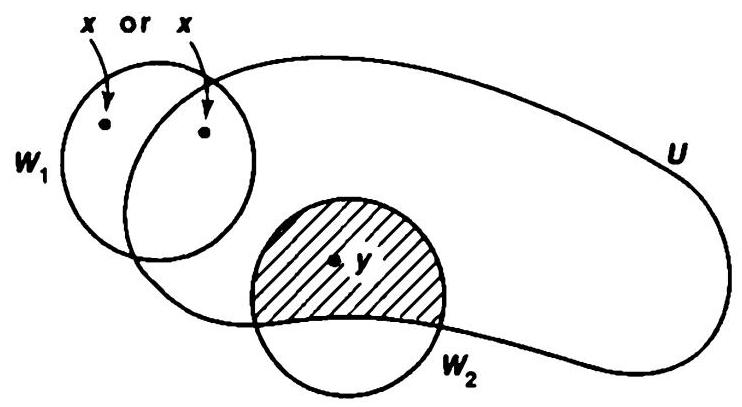
\includegraphics[width=0.6\textwidth]{images/27.3.jpg}
\end{center}
\hspace*{3em} 

Figure 27.3

Let \({x}_{n} = f\left( n\right)\) . Apply Step 1 to the nonempty open set \(U = X\) to choose a nonempty open set \({V}_{1} \subset X\) such that \({\bar{V}}_{1}\) does not contain \({x}_{1}\) . In general, given \({V}_{n - 1}\) open and nonempty, choose \({V}_{n}\) to be a nonempty open set such that \({V}_{n} \subset {V}_{n - 1}\) and \({\bar{V}}_{n}\) does not contain \({x}_{n}\) . Consider the nested sequence

\[
{\bar{V}}_{1} \supset {\bar{V}}_{2} \supset \cdots
\]

of nonempty closed sets of \(X\) . Because \(X\) is compact, there is a point \(x \in \bigcap {\bar{V}}_{n}\) , by Theorem 26.9. Now \(x\) cannot equal \({x}_{n}\) for any \(n\) , since \(x\) belongs to \({V}_{n}\) and \({x}_{n}\) does not.
\end{proof}

\begin{corollary} Every closed interval in \(\mathbb{R}\) is uncountable.
\end{corollary}

\section*{Exercises}

1. Prove that if \(X\) is an ordered set in which every closed interval is compact, then \(X\) has the least upper bound property.

2. Let \(X\) be a metric space with metric \(d\) ; let \(A \subset X\) be nonempty.

(a) Show that \(d\left( {x,A}\right) = 0\) if and only if \(x \in \bar{A}\) .

(b) Show that if \(A\) is compact, \(d\left( {x,A}\right) = d\left( {x,a}\right)\) for some \(a \in A\) .

(c) Define the \(\epsilon\) -neighborhood of \(A\) in \(X\) to be the set

\[
U\left( {A,\epsilon }\right) = \{ x \mid d\left( {x,A}\right) < \epsilon \} .
\]

Show that \(U\left( {A,\epsilon }\right)\) equals the union of the open balls \({B}_{d}\left( {a,\epsilon }\right)\) for \(a \in A\)

(d) Assume that \(A\) is compact; let \(U\) be an open set containing \(A\) . Show that some \(\epsilon\) -neighborhood of \(A\) is contained in \(U\) .

(e) Show the result in (d) need not hold if \(A\) is closed but not compact.

3. Recall that \({\mathbb{R}}_{K}\) denotes \(\mathbb{R}\) in the \(K\) -topology.

(a) Show that \(\left\lbrack {0,1}\right\rbrack\) is not compact as a subspace of \({\mathbb{R}}_{K}\) .

(b) Show that \({\mathbb{R}}_{K}\) is connected. [Hint \(\left( {-\infty,0}\right)\) and \(\left( {0,\infty }\right)\) inherit their usual topologies as subspaces of \({\mathbb{R}}_{K}\) .]

(c) Show that \({\mathbb{R}}_{K}\) is not path connected.

4. Show that a connected metric space having more than one point is uncountable.

5. Let \(X\) be a compact Hausdorff space, let \(\left\{ {A}_{n}\right\}\) be a countable collection of closed sets of \(X\) . Show that if each set \({A}_{n}\) has empty interior in \(X\) , then the union \(\cup {A}_{n}\) has empty interior in \(X\) . [Hint: Imitate the proof of Theorem 27.7.]

This is a special case of the Baire category theorem, which we shall study in Chapter 8.

6. Let \({A}_{0}\) be the closed interval \(\left\lbrack {0,1}\right\rbrack\) in \(\mathbb{R}\) . Let \({A}_{1}\) be the set obtained from \({A}_{0}\) by deleting its ``middle third'' \(\left( {\frac{1}{3},\frac{2}{3}}\right)\) . Let \({A}_{2}\) be the set obtained from \({A}_{1}\) by deleting its ``middle thirds'' \(\left( {\frac{1}{9},\frac{2}{9}}\right)\) and \(\left( {\frac{7}{9},\frac{8}{9}}\right)\) In general, define \({A}_{n}\) by the equation

\[
{A}_{n} = {A}_{n - 1} - \mathop{\bigcup }\limits_{{k = 0}}^{\infty }\left( {\frac{1 + {3k}}{{3}^{n}},\frac{2 + {3k}}{{3}^{n}}}\right) .
\]

The intersection

\[
C = \mathop{\bigcap }\limits_{{n \in {\mathbf{Z}}_{ + }}}{A}_{n}
\]

is called the Cantor set; it is a subspace of \(\left\lbrack {0,1}\right\rbrack\)

(a) Show that \(C\) is totally disconnected.

(b) Show that \(C\) is compact.

(c) Show that each set \({A}_{n}\) is a union of finitely many disjoint closed intervals of length \(1/{3}^{n}\) ; and show that the end points of these intervals lie in \(C\) .

(d) Show that \(C\) has no isolated points.

(e) Conclude that \(C\) is uncountable.

\section*{§ 28 Limit Point Compactness}

As indicated when we first mentioned compact sets, there are other formulations of the notion of compactness that are frequently useful. In this section we introduce one of them. Weaker in general than compactness, it coincides with compactness for metrizable spaces.

\begin{definition} A space \(X\) is said to be limit point compact if every infinite subset of \(X\) has a limit point.
\end{definition}

In some ways this property is more natural and intuitive than that of compactness. In the early days of topology, it was given the name ``compactness,'' while the open covering formulation was called ``bicompactness.'' Later, the word ``compact'' was shifted to apply to the open covering definition, leaving this one to search for a new name It still has not found a name on which everyone agrees On historical grounds, some call it ``Fréchet compactness'', others call it the ``Bolzano-Weierstrass property'' We have invented the term ``limit point compactness'' It seems as good a term as any; at least it describes what the property is about.

\section*{Theorem 28.1. Compactness implies limit point compactness, but not con versely}

\begin{proof}
Let \(X\) be a compact space. Given a subset \(A\) of \(X\) , we wish to prove that if \(A\) is infinite, then \(A\) has a limit point. We prove the contrapositive-if \(A\) has no limit point, then \(A\) must be finite.

So suppose \(A\) has no limit point. Then \(A\) contains all its limit points, so that \(A\) is closed. Furthermore, for each \(a \in A\) we can choose a neighborhood \({U}_{a}\) of \(a\) such that \({U}_{a}\) intersects \(A\) in the point \(a\) alone The space \(X\) is covered by the open set \(X - A\) and the open sets \({U}_{a}\) ; being compact, it can be covered by finitely many of these sets. Since \(X - A\) does not intersect \(A\) , and each set \({U}_{a}\) contains only one point of \(A\) , the set \(A\) must be finite.
\end{proof}

\begin{centeredblock}
\begin{example} Let \(Y\) consist of two points, give \(Y\) the topology consisting of \(Y\) and the empty set Then the space \(X = {\mathbb{Z}}_{ + } \times Y\) is limit point compact, for every nonempty subset of \(X\) has a limit point. It is not compact, for the covering of \(X\) by the open sets \({U}_{n} = \left\lbrack n\right\rbrack \times Y\) has no finite subcollection covering \(X\)
\end{example}
\end{centeredblock}

\begin{centeredblock}
\begin{example} Here is a less trivial example Consider the minimal uncountable well-ordered set \({S}_{\Omega }\) , in the order topology The space \({S}_{\Omega }\) is not compact, since it has no largest element However, it is limit point compact Let \(A\) be an infinite subset of \({S}_{\Omega }\) . Choose a subset \(B\) of \(A\) that is countably infinite Being countable, the set \(B\) has an upper bound \(b\) in \({S}_{\Omega }\) ; then \(B\) is a subset of the interval \(\left\lbrack {{a}_{0},b}\right\rbrack\) of \({S}_{\Omega }\) , where \({a}_{0}\) is the smallest element of \({S}_{\Omega }\) . Since \({S}_{\Omega }\) has the least upper bound property, the interval \(\left\lbrack {{a}_{0},b}\right\rbrack\) is compact By the preceding theorem, \(B\) has a limit point \(x\) in \(\left\lbrack {{a}_{0},b}\right\rbrack\) . The point \(x\) is also a limit point of \(A\) Thus \({S}_{\Omega }\) is limit point compact
\end{example}
\end{centeredblock}

We now show these two versions of compactness coincide for metrizable spaces; for this purpose, we introduce yet another version of compactness called sequential compactness. This result will be used in Chapter 7.

\begin{definition} Let \(X\) be a topological space. If \(\left( {x}_{n}\right)\) is a sequence of points of \(X\) , and if

\[
{n}_{1} < {n}_{2} < \cdots < {n}_{i} < \cdots
\]

is an increasing sequence of positive integers, then the sequence \(\left( {y}_{i}\right)\) defined by setting \({y}_{i} = {x}_{{n}_{i}}\) is called a subsequence of the sequence \(\left( {x}_{n}\right)\) . The space \(X\) is said to be sequentially compact if every sequence of points of \(X\) has a convergent subsequence.
\end{definition}

*Theorem 28.2. Let \(X\) be a metrizable space. Then the following are equivalent:

(1) \(X\) is compact.

(2) \(X\) is limit point compact.

(3) \(X\) is sequentially compact. Proof. We have already proved that (1) \(\Rightarrow\) (2). To show that (2) \(\Rightarrow\) (3), assume that \(X\) is limit point compact. Given a sequence \(\left( {x}_{n}\right)\) of points of \(X\) , consider the set \(A = \left\{ {{x}_{n} \mid n \in {\mathbb{Z}}_{ + }}\right\}\) . If the set \(A\) is finite, then there is a point \(x\) such that \(x = {x}_{n}\) for infinitely many values of \(n\) . In this case, the sequence \(\left( {x}_{n}\right)\) has a subsequence that is constant, and therefore converges trivially. On the other hand, if \(A\) is infinite, then \(A\) has a limit point \(x\) . We define a subsequence of \(\left( {x}_{n}\right)\) converging to \(x\) as follows: First choose \({n}_{1}\) so that

\[
{x}_{{n}_{1}} \in B\left( {x,1}\right) \text{ . }
\]

Then suppose that the positive integer \({n}_{i - 1}\) is given. Because the ball \(B\left( {x,1/i}\right)\) intersects \(A\) in infinitely many points, we can choose an index \({n}_{i} > {n}_{i - 1}\) such that

\[
{x}_{{n}_{i}} \in B\left( {x,1/\iota }\right) \text{ . }
\]

Then the subsequence \({x}_{{n}_{1}},{x}_{{n}_{2}},\ldots\) converges to \(x\) .

Finally, we show that \(\left( 3\right) \Rightarrow \left( 1\right)\) . This is the hardest part of the proof.

First, we show that if \(X\) is sequentially compact, then the Lebesgue number lemma holds for \(X\) . (This would follow from compactness, but compactness is what we are trying to prove!) Let \(\mathcal{A}\) be an open covering of \(X\) . We assume that there is no \(\delta > 0\) such that each set of diameter less than \(\delta\) has an element of \(\mathcal{A}\) containing it, and derive a contradiction.

Our assumption implies in particular that for each positive integer \(n\) , there exists a set of diameter less than \(1/n\) that is not contained in any element of \(\mathcal{A}\) ; let \({C}_{n}\) be such a set. Choose a point \({x}_{n} \in {C}_{n}\) , for each \(n\) . By hypothesis, some subsequence \(\left( {x}_{{n}_{i}}\right)\) of the sequence \(\left( {x}_{n}\right)\) converges, say to the point \(a\) . Now \(a\) belongs to some element \(A\) of the collection \(\mathcal{A}\) ; because \(A\) is open, we may choose an \(\epsilon > 0\) such that \(B\left( {a,\epsilon }\right) \subset A\) . If \(i\) is large enough that \(1/{n}_{i} < \epsilon /2\) , then the set \({C}_{{n}_{i}}\) lies in the \(\epsilon /2\) -neighborhood of \({x}_{{n}_{i}}\) ; if \(i\) is also chosen large enough that \(d\left( {{x}_{{n}_{i}},a}\right) < \epsilon /2\) , then \({C}_{{n}_{i}}\) lies in the \(\epsilon\) -neighborhood of \(a\) . But this means that \({C}_{{n}_{t}} \subset A\) , contrary to hypothesis.

Second, we show that if \(X\) is sequentially compact, then given \(\epsilon > 0\) , there exists a finite covering of \(X\) by open \(\epsilon\) -balls. Once again, we proceed by contradiction. Assume that there exists an \(\epsilon > 0\) such that \(X\) cannot be covered by finitely many \(\epsilon\) -balls. Construct a sequence of points \({x}_{n}\) of \(X\) as follows: First, choose \({x}_{1}\) to be any point of \(X\) . Noting that the ball \(B\left( {{x}_{1},\epsilon }\right)\) is not all of \(X\) (otherwise \(X\) could be covered by a single \(\epsilon\) -ball), choose \({x}_{2}\) to be a point of \(X\) not in \(B\left( {{x}_{1},\epsilon }\right)\) . In general, given \({x}_{1},\ldots,{x}_{n}\) , choose \({x}_{n + 1}\) to be a point not in the union

\[
B\left( {{x}_{1},\epsilon }\right) \cup \cdots \cup B\left( {{x}_{n},\epsilon }\right) ,
\]

using the fact that these balls do not cover \(X\) . Note that by construction \(d\left( {{x}_{n + 1},{x}_{i}}\right) \geq\) \(\epsilon\) for \(i = 1,\ldots,n\) . Therefore, the sequence \(\left( {x}_{n}\right)\) can have no convergent subsequence; in fact, any ball of radius \(\epsilon /2\) can contain \({x}_{n}\) for at most one value of \(n\) .

Finally, we show that if \(X\) is sequentially compact, then \(X\) is compact. Let \(\mathcal{A}\) be an open covering of \(X\) . Because \(X\) is sequentially compact, the open covering \(\mathcal{A}\) has a Lebesgue number \(\delta\) . Let \(\epsilon = \delta /3\) ; use sequential compactness of \(X\) to find a finite covering of \(X\) by open \(\epsilon\) -balls. Each of these balls has diameter at most \({2\delta }/3\) , so it lies in an element of \(\mathcal{A}\) . Choosing one such element of \(\mathcal{A}\) for each of these \(\epsilon\) -balls, we obtain a finite subcollection of \(\mathcal{A}\) that covers \(X\) .

\begin{centeredblock}
\begin{example} Recall that \({\bar{S}}_{\Omega }\) denotes the minimal uncountable well-ordered set \({S}_{\Omega }\) with the point \(\Omega\) adjoined. (In the order topology, \(\Omega\) is a limit point of \({S}_{\Omega }\) , which is why we introduced the notation \({\bar{S}}_{\Omega }\) for \({S}_{\Omega } \cup \{ \Omega \}\) , back in \(\$ {10})\) It is easy to see that the space \({\bar{S}}_{\Omega }\) is not metrizable, for it does not satisfy the sequence lemma: The point \(\Omega\) is a limit point of \({S}_{\Omega }\) , but it is not the limit of a sequence of points of \({S}_{\Omega }\) , for any sequence of points of \({S}_{\Omega }\) has an upper bound in \({S}_{\Omega }\) The space \({S}_{\Omega }\) , on the other hand, does satisfy the sequence lemma, as you can readily check Nevertheless, \({S}_{\Omega }\) is not metrizable, for it is limit point compact but not compact.
\end{example}
\end{centeredblock}

\section*{Exercises}

1. Give \({\left\lbrack 0,1\right\rbrack }^{\omega }\) the uniform topology. Find an infinite subset of this space that has no limit point

2. Show that \(\left\lbrack {0,1}\right\rbrack\) is not limit point compact as a subspace of \({\mathbb{R}}_{\ell }\) .

3. Let \(X\) be limit point compact.

(a) If \(f \cdot X \rightarrow Y\) is continuous, does it follow that \(f\left( X\right)\) is limit point compact?

(b) If \(A\) is a closed subset of \(X\) , does it follow that \(A\) is limit point compact?

(c) If \(X\) is a subspace of the Hausdorff space \(Z\) , does it follow that \(X\) is closed in \(Z\) ?

We comment that it is not in general true that the product of two limit point compact spaces is limit point compact, even if the Hausdorff condition is assumed. But the examples are fairly sophisticated. See \cite{SteenSeebach1970}, Example II2.

4. A space \(X\) is said to be countably compact if every countable open covering of \(X\) contains a finite subcollection that covers \(X\) . Show that for a \({T}_{1}\) space \(X\) , countable compactness is equivalent to limit point compactness. [Hint: If no finite subcollection of \({U}_{n}\) covers \(X\) , choose \({x}_{n} \notin {U}_{1} \cup \cdots \cup {U}_{n}\) , for each \(n\) .]

5. Show that \(X\) is countably compact if and only if every nested sequence \({C}_{1} \supset\) \({C}_{2} \supset\) - of closed nonempty sets of \(X\) has a nonempty intersection.

6. Let(X, d)be a metric space. If \(f: X \rightarrow X\) satisfies the condition

\[
d\left( {f\left( x\right) ,f\left( y\right) }\right) = d\left( {x,y}\right)
\]

for all \(x,y \in X\) , then \(f\) is called an isometry of \(X\) . Show that if \(f\) is an isometry and \(X\) is compact, then \(f\) is bijective and hence a homeomorphism. [Hint: If \(a \notin f\left( X\right)\) , choose \(\epsilon\) so that the \(\epsilon\) -neighborhood of \(a\) is disjoint from \(f\left( X\right)\) Set \({x}_{1} = a\) , and \({x}_{n + 1} = f\left( {x}_{n}\right)\) in general. Show that \(d\left( {{x}_{n},{x}_{m}}\right) \geq \epsilon\) for \(n \neq m\) .]

7. Let(X, d)be a metric space. If \(f\) satisfies the condition

\[
d\left( {f\left( x\right) ,f\left( y\right) }\right) < d\left( {x,y}\right)
\]

for all \(x,y \in X\) with \(x \neq y\) , then \(f\) is called a shrinking map If there is a number \(\alpha < 1\) such that

\[
d\left( {f\left( x\right) ,f\left( y\right) }\right) \leq {\alpha d}\left( {x,y}\right)
\]

for all \(x,y \in X\) , then \(f\) is called a contraction. A fixed point of \(f\) is a point \(x\) such that \(f\left( x\right) = x\)

(a) If \(f\) is a contraction and \(X\) is compact, show \(f\) has a unique fixed point. [Hint: Define \({f}^{1} = f\) and \({f}^{n + 1} = f \circ {f}^{n}\) . Consider the intersection \(A\) of the sets \(\left. {{A}_{n} = {f}^{n}\left( X\right) \text{ . }}\right\rbrack\)

(b) Show more generally that if \(f\) is a shrinking map and \(X\) is compact, then \(f\) has a unique fixed point. [Hint: Let \(A\) be as before. Given \(x \in A\) , choose \({x}_{n}\) so that \(x = {f}^{n + 1}\left( {x}_{n}\right)\) . If \(a\) is the limit of some subsequence of the sequence \({y}_{n} = {f}^{n}\left( {x}_{n}\right)\) , show that \(a \in A\) and \(f\left( a\right) = x\) . Conclude that \(A = f\left( A\right)\) , so that diam \(A = 0\) .]

(c) Let \(X = \left\lbrack {0,1}\right\rbrack\) . Show that \(f\left( x\right) = x - {x}^{2}/2\) maps \(X\) into \(X\) and is a shrinking map that is not a contraction. [Hint Use the mean-value theorem of calculus.]

(d) The result in (a) holds if \(X\) is a complete metric space, such as \(\mathbb{R}\) ; see the exercises of \(§{43}\) . The result in (b) does not. Show that the map \(f \cdot \mathbb{R} \rightarrow\) \(\mathbb{R}\) given by \(f\left( x\right) = \left\lbrack {x + {\left( {x}^{2} + 1\right) }^{1/2}}\right\rbrack /2\) is a shrinking map that is not a contraction and has no fixed point.

\section*{§ 29 Local Compactness}

In this section we study the notion of local compactness, and we prove the basic theorem that any locally compact Hausdorff space can be imbedded in a certain compact Hausdorff space that is called its one-point compactification.

\begin{definition} A space \(X\) is said to be locally compact at \(x\) if there is some compact subspace \(C\) of \(X\) that contains a neighborhood of \(x\) . If \(X\) is locally compact at each of its points, \(X\) is said simply to be locally compact.
\end{definition}

Note that a compact space is automatically locally compact.

\begin{centeredblock}
\begin{example} The real line \(\mathbf{R}\) is locally compact. The point \(x\) lies in some interval(a, b), which in turn is contained in the compact subspace \(\left\lbrack {a,b}\right\rbrack\) The subspace \(\mathbb{Q}\) of rational numbers is not locally compact, as you can check.
\end{example}
\end{centeredblock}

\begin{centeredblock}
\begin{example} The space \({\mathbb{R}}^{n}\) is locally compact, the point \(x\) lies in some basis element \(\left( {{a}_{1},{b}_{1}}\right) \times \cdot \times \left( {{a}_{n},{b}_{n}}\right)\) , which in turn lies in the compact subspace \(\left\lbrack {{a}_{1},{b}_{1}}\right\rbrack \times \cdot \times \left\lbrack {{a}_{n},{b}_{n}}\right\rbrack\) . The space \({\mathbb{R}}^{\omega }\) is not locally compact, none of its basis elements are contained in compact subspaces For if

\[
B = \left( {{a}_{1},{b}_{1}}\right) \times \cdot \times \left( {{a}_{n},{b}_{n}}\right) \times \mathbb{R} \times \cdot \times \mathbb{R} \times
\]

were contained in a compact subspace, then its closure

\[
\bar{B} = \left\lbrack {{a}_{1},{b}_{1}}\right\rbrack \times \; \cdot \times \left\lbrack {{a}_{n},{b}_{n}}\right\rbrack \times \mathbb{R} \times.
\]

would be compact, which it is not.
\end{example}
\end{centeredblock}

\begin{centeredblock}
\begin{example} Every simply ordered set \(X\) having the least upper bound property is locally compact: Given a basis element for \(X\) , it is contained in a closed interval in \(X\) , which is compact.
\end{example}
\end{centeredblock}

Two of the most well-behaved classes of spaces to deal with in mathematics are the metrizable spaces and the compact Hausdorff spaces. Such spaces have many useful properties, which one can use in proving theorems and making constructions and the like. If a given space is not of one of these types, the next best thing one can hope for is that it is a subspace of one of these spaces. Of course, a subspace of a metrizable space is itself metrizable, so one does not get any new spaces in this way. But a subspace of a compact Hausdorff space need not be compact. Thus arises the question: Under what conditions is a space homeomorphic with a subspace of a compact Hausdorff space? We give one answer here. We shall return to this question in Chapter 5 when we study compactifications in general.

\begin{theorem} Let \(X\) be a space. Then \(X\) is locally compact Hausdorff if and only if there exists a space \(Y\) satisfying the following conditions:

(1) \(X\) is a subspace of \(Y\) .

(2) The set \(Y - X\) consists of a single point.

(3) \(Y\) is a compact Hausdorff space.

If \(Y\) and \({Y}^{\prime }\) are two spaces satisfying these conditions, then there is a homeomorphism of \(Y\) with \({Y}^{\prime }\) that equals the identity map on \(X\) .

\end{theorem}
\begin{proof}
Step 1. We first verify uniqueness. Let \(Y\) and \({Y}^{\prime }\) be two spaces satisfying these conditions. Define \(h: Y \rightarrow {Y}^{\prime }\) by letting \(h\) map the single point \(p\) of \(Y - X\) to the point \(q\) of \({Y}^{\prime } - X\) , and letting \(h\) equal the identity on \(X\) . We show that if \(U\) is open in \(Y\) , then \(h\left( U\right)\) is open in \({Y}^{\prime }\) . Symmetry then implies that \(h\) is a homeomorphism.

First, consider the case where \(U\) does not contain \(p\) . Then \(h\left( U\right) = U\) . Since \(U\) is open in \(Y\) and is contained in \(X\) , it is open in \(X\) . Because \(X\) is open in \({Y}^{\prime }\) , the set \(U\) is also open in \({Y}^{\prime }\) , as desired.

Second, suppose that \(U\) contains \(p\) . Since \(C = Y - U\) is closed in \(Y\) , it is compact as a subspace of \(Y\) . Because \(C\) is contained in \(X\) , it is a compact subspace of \(X\) . Then because \(X\) is a subspace of \({Y}^{\prime }\) , the space \(C\) is also a compact subspace of \({Y}^{\prime }\) . Because \({Y}^{\prime }\) is Hausdorff, \(C\) is closed in \({Y}^{\prime }\) , so that \(h\left( U\right) = {Y}^{\prime } - C\) is open in \({Y}^{\prime }\) , as desired

Step 2 Now we suppose \(X\) is locally compact Hausdorff and construct the space \(Y\) . Step I gives us an idea how to proceed. Let us take some object that is not a point of \(X\) , denote it by the symbol \(\infty\) for convenience, and adjoin it to \(X\) , forming the set \(Y = X \cup \{ \infty \}\) . Topologize \(Y\) by defining the collection of open sets of \(Y\) to consist of (1) all sets \(U\) that are open in \(X\) , and (2) all sets of the form \(Y - C\) , where \(C\) is a compact subspace of \(X\) .

We need to check that this collection is, in fact, a topology on \(Y\) The empty set is a set of type (1), and the space \(Y\) is a set of type (2). Checking that the intersection of two open sets is open involves three cases:

\[
{U}_{1} \cap {U}_{2}\;\text{ is of type (1). }
\]

\[
\left( {Y - {C}_{1}}\right) \cap \left( {Y - {C}_{2}}\right) = Y - \left( {{C}_{1} \cup {C}_{2}}\right) \;\text{ is of type (2). }
\]

\[
{U}_{1} \cap \left( {Y - {C}_{1}}\right) = {U}_{1} \cap \left( {X - {C}_{1}}\right) \;\text{ is of type }\left( l\right) ,
\]

because \({C}_{1}\) is closed in \(X\) . Similarly, one checks that the union of any collection of open sets is open.

\[
\bigcup {U}_{\alpha } = U
\]

\[
\bigcup \left( {Y - {C}_{\beta }}\right) = Y - \left( {\bigcap {C}_{\beta }}\right) = Y - C
\]
 is of type (2).

\[
\left( {\bigcup {U}_{\alpha }}\right) \cup \left( {\bigcup \left( {Y - {C}_{\beta }}\right) }\right) = U \cup \left( {Y - C}\right) = Y - \left( {C - U}\right)
\]

which is of type (2) because \(C - U\) is a closed subspace of \(C\) and therefore compact.

Now we show that \(X\) is a subspace of \(Y\) . Given any open set of \(Y\) , we show its intersection with \(X\) is open in \(X\) . If \(U\) is of type (1), then \(U \cap X = U\) ; if \(Y - C\) is of type (2), then \(\left( {Y - C}\right) \cap X = X - C\) ; both of these sets are open in \(X\) . Conversely, any set open in \(X\) is a set of type (1) and therefore open in \(Y\) by definition.

To show that \(Y\) is compact, let \(\mathcal{A}\) be an open covering of \(Y\) . The collection \(\mathcal{A}\) must contain an open set of type (2), say \(Y - C\) , since none of the open sets of type (1) contain the point \(\infty\) . Take all the members of \(\mathcal{A}\) different from \(Y - C\) and intersect them with \(X\) ; they form a collection of open sets of \(X\) covering \(C\) . Because \(C\) is compact, finitely many of them cover \(C\) ; the corresponding finite collection of elements of \(\mathcal{A}\) will, along with the element \(Y - C\) , cover all of \(Y\)

To show that \(Y\) is Hausdorff, let \(x\) and \(y\) be two points of \(Y\) . If both of them lie in \(X\) , there are disjoint sets \(U\) and \(V\) open in \(X\) containing them, respectively. On the other hand, if \(x \in X\) and \(y = \infty\) , we can choose a compact set \(C\) in \(X\) containing a neighborhood \(U\) of \(x\) . Then \(U\) and \(Y - C\) are disjoint neighborhoods of \(x\) and \(\infty\) , respectively, in \(Y\) .

Step 3. Finally, we prove the converse. Suppose a space \(Y\) satisfying conditions (1)-(3) exists. Then \(X\) is Hausdorff because it is a subspace of the Hausdorff space \(Y\) . Given \(x \in X\) , we show \(X\) is locally compact at \(x\) Choose disjoint open sets \(U\) and \(V\) of \(Y\) containing \(x\) and the single point of \(Y - X\) , respectively Then the set \(C = Y - V\) is closed in \(Y\) , so it is a compact subspace of \(Y\) Since \(C\) lies in \(X\) , it is also compact as a subspace of \(X\) ; it contains the neighborhood \(U\) of \(x\) .

If \(X\) itself should happen to be compact, then the space \(Y\) of the preceding theorem is not very interesting, for it is obtained from \(X\) by adjoining a single isolated point. However, if \(X\) is not compact, then the point of \(Y - X\) is a limit point of \(X\) , so that \(\bar{X} = Y\)
\end{proof}

\begin{definition} If \(Y\) is a compact Hausdorff space and \(X\) is a proper subspace of \(Y\) whose closure equals \(Y\) , then \(Y\) is said to be a compactification of \(X\) . If \(Y - X\) equals a single point, then \(Y\) is called the one-point compactification of \(X\) .
\end{definition}

We have shown that \(X\) has a one-point compactification \(Y\) if and only if \(X\) is a locally compact Hausdorff space that is not itself compact. We speak of \(Y\) as ``the'' one-point compactification because \(Y\) is uniquely determined up to a homeomorphism.

\begin{centeredblock}
\begin{example} The one-point compactification of the real line \(\mathbb{R}\) is homeomorphic with the circle, as you may readily check Similarly, the one-point compactification of \({\mathbb{R}}^{2}\) is homeomorphic to the sphere \({S}^{2}\) . If \({\mathbb{R}}^{2}\) is looked at as the space \(\mathbb{C}\) of complex numbers, then \(\mathbb{C} \cup \{ \infty \}\) is called the Riemann sphere, or the extended complex plane
\end{example}
\end{centeredblock}

In some ways our definition of local compactness is not very satisfying. Usually one says that a space \(X\) satisfies a given property ``locally'' if every \(x \in X\) has ``arbitrarily small'' neighborhoods having the given property. Our definition of local compactness has nothing to do with ``arbitrarily small'' neighborhoods, so there is some question whether we should call it local compactness at all.

Here is another formulation of local compactness, one more truly ``local'' in nature; it is equivalent to our definition when \(X\) is Hausdorff.

\begin{theorem} Let \(X\) be a Hausdorff space Then \(X\) is locally compact if and only if given \(x\) in \(X\) , and given a neighborhood \(U\) of \(x\) , there is a neighborhood \(V\) of \(x\) such that \(\bar{V}\) is compact and \(\bar{V} \subset U\)

\end{theorem}
\begin{proof}
Clearly this new formulation implies local compactness; the set \(C = \bar{V}\) is the desired compact set containing a neighborhood of \(x\) . To prove the converse, suppose \(X\) is locally compact, let \(x\) be a point of \(X\) and let \(U\) be a neighborhood of \(x\) . Take the one-point compactification \(Y\) of \(X\) , and let \(C\) be the set \(Y - U\) Then \(C\) is closed in \(Y\) , so that \(C\) is a compact subspace of \(Y\) . Apply Lemma 26 4 to choose disjoint open sets \(V\) and \(W\) containing \(x\) and \(C\) , respectively. Then the closure \(\bar{V}\) of \(V\) in \(Y\) is compact, furthermore, \(\bar{V}\) is disjoint from \(C\) , so that \(\bar{V} \subset U\) , as desired.
\end{proof}

\begin{corollary} Let \(X\) be locally compact Hausdorff, let \(A\) be a subspace of \(X\) If \(A\) is closed in \(X\) or open in \(X\) , then \(A\) is locally compact.
\end{corollary}

\begin{proof}
Suppose that \(A\) is closed in \(X\) . Given \(x \in A\) , let \(C\) be a compact subspace of \(X\) containing the neighborhood \(U\) of \(x\) in \(X\) . Then \(C \cap A\) is closed in \(C\) and thus compact, and it contains the neighborhood \(U \cap A\) of \(x\) in \(A\) . (We have not used the Hausdorff condition here.)

Suppose now that \(A\) is open in \(X\) . Given \(x \in A\) , we apply the preceding theorem to choose a neighborhood \(V\) of \(x\) in \(X\) such that \(\bar{V}\) is compact and \(\bar{V} \subset A\) . Then \(C = \bar{V}\) is a compact subspace of \(A\) containing the neighborhood \(V\) of \(x\) in \(A\) .
\end{proof}

\begin{corollary} A space \(X\) is homeomorphic to an open subspace of a compact Hausdorff space if and only if \(X\) is locally compact Hausdorff.
\end{corollary}

\begin{proof}
This follows from Theorem 29 1 and Corollary 29.3.
\end{proof}

\section*{Exercises}

1. Show that the rationals \(\mathbb{Q}\) are not locally compact.

2. Let \(\left\{ {X}_{\alpha }\right\}\) be an indexed family of nonempty spaces.

(a) Show that if \(\prod {X}_{\alpha }\) is locally compact, then each \({X}_{\alpha }\) is locally compact and \({X}_{\alpha }\) is compact for all but finitely many values of \(\alpha\) .

(b) Prove the converse, assuming the Tychonoff theorem.

3. Let \(X\) be a locally compact space. If \(f: X \rightarrow Y\) is continuous, does it follow that \(f\left( X\right)\) is locally compact? What if \(f\) is both continuous and open? Justify your answer.

4. Show that \({\left\lbrack 0,1\right\rbrack }^{\omega }\) is not locally compact in the uniform topology.

5. If \(f: {X}_{1} \rightarrow {X}_{2}\) is a homeomorphism of locally compact Hausdorff spaces, show \(f\) extends to a homeomorphism of their one-point compactifications.

6. Show that the one-point compactification of \(\mathbb{R}\) is homeomorphic with the circle \({S}^{1}\) .

7. Show that the one-point compactification of \({S}_{\Omega }\) is homeomorphic with \({\bar{S}}_{\Omega }\) .

8. Show that the one-point compactification of \({\mathbb{Z}}_{ + }\) is homeomorphic with the subspace \(\{ 0\} \cup \left\{ {1/n \mid n \in {\mathbb{Z}}_{ + }}\right\}\) of \(\mathbb{R}\) .

9. Show that if \(G\) is a locally compact topological group and \(H\) is a subgroup, then \(G/H\) is locally compact.

10. Show that if \(X\) is a Hausdorff space that is locally compact at the point \(x\) , then for each neighborhood \(U\) of \(x\) , there is a neighborhood \(V\) of \(x\) such that \(\bar{V}\) is compact and \(\bar{V} \subset U\) .

-11. Prove the following:

(a) Lemma. If \(p: X \rightarrow Y\) is a quotient map and if \(Z\) is a locally compact Hausdorff space, then the map

\[
\pi = p \times {i}_{Z} : X \times Z \rightarrow Y \times Z
\]

is a quotient map.

[Hint: If \({\pi }^{-1}\left( A\right)\) is open and contains \(x \times y\) , choose open sets \({U}_{1}\) and \(V\) with \(\bar{V}\) compact, such that \(x \times y \in {U}_{1} \times V\) and \({U}_{1} \times \bar{V} \subset {\pi }^{-1}\left( A\right)\) . Given \({U}_{i} \times \bar{V} \subset {\pi }^{-1}\left( A\right)\) , use the tube lemma to choose an open set \({U}_{i + 1}\) containing \({p}^{-1}\left( {p\left( {U}_{i}\right) }\right)\) such that \({U}_{i + 1} \times \bar{V} \subset {\pi }^{-1}\left( A\right)\) . Let \(U = \bigcup {U}_{i}\) ; show that \(U \times V\) is a saturated neighborhood of \(x \times y\) that is contained in \({\pi }^{-1}\left( A\right)\) .

An entirely different proof of this result will be outlined in the exercises of §46.

(b) Theorem. Let \(p: A \rightarrow B\) and \(q: C \rightarrow D\) be quotient maps. If \(B\) and \(C\) are locally compact Hausdorff spaces, then \(p \times q: A \times C \rightarrow B \times D\) is a quotient map.

\section*{* Supplementary Exercises: Nets}

We have already seen that sequences are ``adequate'' to detect limit points, continuous functions, and compact sets in metrizable spaces. There is a generalization of the notion of sequence, called a net, that will do the same thing for an arbitrary topological space. We give the relevant definitions here, and leave the proofs as exercises. Recall that a relation \(\preccurlyeq\) on a set \(A\) is called a partial order relation if the following conditions hold:

(1) \(\alpha \preccurlyeq \alpha\) for all \(\alpha\) .

(2) If \(\alpha \preccurlyeq \beta\) and \(\beta \preccurlyeq \alpha\) , then \(\alpha = \beta\) .

(3) If \(\alpha \preccurlyeq \beta\) and \(\beta \preccurlyeq \gamma\) , then \(\alpha \preccurlyeq \gamma\) .

Now we make the following definition:

A directed set \(J\) is a set with a partial order \(\preccurlyeq\) such that for each pair \(\alpha,\beta\) of elements of \(J\) , there exists an element \(\gamma\) of \(J\) having the property that \(\alpha \preccurlyeq \gamma\) and \(\beta \preccurlyeq \gamma\) .

1. Show that the following are directed sets:

(a) Any simply ordered set, under the relation \(\leq\) .

(b) The collection of all subsets of a set \(S\) , partially ordered by inclusion (that is, \(A \preccurlyeq B\) if \(A \subset B\) ).

(c) A collection \(\mathcal{A}\) of subsets of \(S\) that is closed under finite intersections, partially ordered by reverse inclusion (that is \(A \preccurlyeq B\) if \(A \supset B\) ).

(d) The collection of all closed subsets of a space \(X\) , partially ordered by inclusion.

2. A subset \(K\) of \(J\) is said to be cofinal in \(J\) if for each \(\alpha \in J\) , there exists \(\beta \in K\) such that \(\alpha \preccurlyeq \beta\) . Show that if \(J\) is a directed set and \(K\) is cofinal in \(J\) , then \(K\) is a directed set.

3. Let \(X\) be a topological space. A net in \(X\) is a function \(f\) from a directed set \(J\) into \(X\) . If \(\alpha \in J\) , we usually denote \(f\left( \alpha \right)\) by \({x}_{\alpha }\) . We denote the net \(f\) itself by the symbol \({\left( {x}_{\alpha }\right) }_{\alpha \in J}\) , or merely by \(\left( {x}_{\alpha }\right)\) if the index set is understood.

The net \(\left( {x}_{\alpha }\right)\) is said to converge to the point \(x\) of \(X\) (written \({x}_{\alpha } \rightarrow x\) ) if for each neighborhood \(U\) of \(x\) , there exists \(\alpha \in J\) such that

\[
\alpha \preccurlyeq \beta \Rightarrow {x}_{\beta } \in U
\]

Show that these definitions reduce to familiar ones when \(J = {\mathbb{Z}}_{ + }\) .

4. Suppose that

\[
{\left( {x}_{\alpha }\right) }_{\alpha \in J} \rightarrow x\text{ in }X\text{ and }{\left( {y}_{\alpha }\right) }_{\alpha \in J} \rightarrow y\text{ in }Y.
\]

Show that \(\left( {{x}_{\alpha } \times {y}_{\alpha }}\right) \rightarrow x \times y\) in \(X \times Y\) .

5. Show that if \(X\) is Hausdorff, a net in \(X\) converges to at most one point.

6. Theorem. Let \(A \in X\) . Then \(x \in \bar{A}\) if and only if there is a net of points of \(A\) converging to \(x\) .

[Hint: To prove the implication \(\Rightarrow\) , take as index set the collection of all neighborhoods of \(x\) , partially ordered by reverse inclusion.]

7. Theorem Let \(f: X \rightarrow Y\) . Then \(f\) is continuous if and only if for every convergent net \(\left( {x}_{\alpha }\right)\) in \(X\) , converging to \(x\) , say, the net \(\left( {f\left( {x}_{\alpha }\right) }\right)\) converges to \(f\left( x\right)\) .

8. Let \(f: J \rightarrow X\) be a net in \(X\) ; let \(f\left( \alpha \right) = {x}_{\alpha }\) . If \(K\) is a directed set and \(g: K \rightarrow J\) is a function such that

(i) \(i \preccurlyeq j \Rightarrow g\left( \iota \right) \preccurlyeq g\left( j\right)\) ,

(ii) \(g\left( K\right)\) is cofinal in \(J\) ,

then the composite function \(f \circ g: K \rightarrow X\) is called a subnet of \(\left( {x}_{\alpha }\right)\) . Show that if the net \(\left( {x}_{\alpha }\right)\) converges to \(x\) , so does any subnet.

9. Let \({\left( {x}_{\alpha }\right) }_{\alpha \in J}\) be a net in \(X\) . We say that \(x\) is an accumulation point of the net \(\left( {x}_{\alpha }\right)\) if for each neighborhood \(U\) of \(x\) , the set of those \(\alpha\) for which \({x}_{\alpha } \in U\) is cofinal in \(J\) .

\begin{lemma} The net \(\left( {x}_{\alpha }\right)\) has the point \(x\) as an accumulation point if and only if some subnet of \(\left( {x}_{\alpha }\right)\) converges to \(x\) .
\end{lemma}

[Hint: To prove the implication \(\Rightarrow\) , let \(K\) be the set of all pairs \(\left( {\alpha,U}\right)\) where \(\alpha \in J\) and \(U\) is a neighborhood of \(x\) containing \({x}_{\alpha }\) . Define \(\left( {\alpha,U}\right) \preccurlyeq \left( {\beta,V}\right)\) if \(\alpha \preccurlyeq \beta\) and \(V \subset U\) . Show that \(K\) is a directed set and use it to define the subnet.]

10. Theorem. X is compact if and only if every net in \(X\) has a convergent subnet. [Hint: To prove the implication \(\Rightarrow\) , let \({B}_{\alpha } = \left\{ {{x}_{\beta } \mid \alpha \preccurlyeq \beta }\right\}\) and show that \(\left\{ {B}_{\alpha }\right\}\) has the finite intersection property. To prove \(\Leftarrow\) , let \(\mathcal{A}\) be a collection of closed sets having the finite intersection property, and let \(\mathcal{B}\) be the collection of all finite intersections of elements of \(\mathcal{A}\) , partially ordered by reverse inclusion.]

11. Corollary. Let \(G\) be a topological group; let \(A\) and \(B\) be subsets of \(G\) . If \(A\) is closed in \(G\) and \(B\) is compact, then \(A \cdot B\) is closed in \(G\) . [Hint: First give a proof using sequences, assuming that \(G\) is metrizable.]

12. Check that the preceding exercises remain correct if condition (2) is omitted from the definition of directed set. Many mathematicians use the term ``directed set'' in this more general sense.
\chapteropening[Countability and Separation Axioms]{Countability \\and Separation Axioms}

The concepts we are going to introduce now, unlike compactness and connectedness, do not arise naturally from the study of calculus and analysis. They arise instead from a deeper study of topology itself. Such problems as imbedding a given space in a metric space or in a compact Hausdorff space are basically problems of topology rather than analysis. These particular problems have solutions that involve the countability and separation axioms.

We have already introduced the first countability axiom; it arose in connection with our study of convergent sequences in \S\ 21. We have also studied one of the separation axioms-the Hausdorff axiom, and mentioned another-the \(T_{1}\) axiom. In this chapter we shall introduce other, and stronger, axioms like these and explore some of their consequences. Our basic goal is to prove the \idx[Urysohn metrization theorem]{Urysohn metrization theorem}. It says that if a topological space \(X\) satisfies a certain countability axiom (the second) and a certain separation axiom (the \idx[regularity]{Regularity} axiom), then \(X\) can be imbedded in a metric space and is thus metrizable.

Another imbedding theorem, important to geometers, appears in the last section of the chapter. Given a space that is a compact \idx[manifold]{Manifold} (the higher-dimensional analogue of a \idx[surface]{Surface}), we show that it can be imbedded in some finite-dimensional euclidean space.

\booksection{30}{The Countability Axioms}

Recall the definition we gave in \S\ 21.

\begin{definition}
 A space \(X\) is said to have a \idx[countable basis]{Countable basis} at \(x\) if there is a countable collection \(\mathcal{B}\) of neighborhoods of \(x\) such that each neighborhood of \(x\) contains at least one of the elements of \(\mathcal{B}\). A space that has a countable basis at each of its points is said to satisfy the first countability axiom, or to be first-countable.
\end{definition}

We have already noted that every metrizable space satisfies this axiom; see \S\ 21.

The most useful fact concerning spaces that satisfy this axiom is the fact that in such a space, convergent sequences are adequate to detect limit points of sets and to check continuity of functions. We have noted this before; now we state it formally as a theorem:

\begin{theorem}
\label{thm:\thetheorem}
 Let \(X\) be a topological space.

(a) Let \(A\) be a subset of \(X\). If there is a sequence of points of \(A\) converging to \(x\), then \(x \in \bar{A}\) ; the converse holds if \(X\) is first-countable.

(b) Let \(f : X \rightarrow Y\). If \(f\) is continuous, then for every convergent sequence \(x_{n} \rightarrow x\) in \(X\), the sequence \(f( x_{n})\) converges to \(f(x)\). The converse holds if \(X\) is first-countable.

\end{theorem}

The proof is a direct generalization of the proof given in \S\ 21 under the hypothesis of metrizability, so it will not be repeated here.

Of much greater importance than the first countability axiom is the following:

\begin{definition}
 If a space \(X\) has a countable basis for its topology, then \(X\) is said to satisfy the second countability axiom, or to be second-countable.
\end{definition}

Obviously, the second axiom implies the first: if \(\mathcal{B}\) is a countable basis for the topology of \(X\), then the subset of \(\mathcal{B}\) consisting of those basis elements containing the point \(x\) is a countable basis at \(x\). The second axiom is, in fact, much stronger than the first; it is so strong that not even every metric space satisfies it.

Why then is this second axiom interesting? Well, for one thing, many familiar spaces do satisfy it. For another, it is a crucial hypothesis used in proving such theorems as the Urysohn metrization theorem, as we shall see.

\begin{centeredblock}
\begin{example}
\label{ex:\thesection.\theexample}
 The real line \(\mathbb{R}\) has a countable basis-the collection of all open intervals \((a, b)\) with rational end points. Likewise, \(\mathbb{R}^{n}\) has a countable basis—the collection of all products of intervals having rational end points. Even \(\mathbb{R}^{\omega }\) has a countable basis-the collection of all products \(\mathop{\prod }\limits_{{n \in {\mathbb{Z}}_{ + }}}U_{n}\), where \(U_{n}\) is an open interval with rational end points for finitely many values of \(n\), and \(U_{n} = \mathbb{R}\) for all other values of \(n\).
\end{example}
\end{centeredblock}

\begin{centeredblock}
\begin{example}
\label{ex:\thesection.\theexample}
 In the uniform topology, \(\mathbb{R}^{\omega }\) satisfies the first countability axiom (being metrizable). However, it does not satisfy the second. To verify this fact, we first show that if \(X\) is a space having a countable basis \(\mathcal{B}\), then any discrete subspace \(A\) of \(X\) must be countable. Choose, for each \(a \in A\), a basis element \(B_{a}\) that intersects \(A\) in the point \(a\) alone. If \(a\) and \(b\) are distinct points of \(A\), the sets \(B_{a}\) and \(B_{b}\) are different, since the first contains \(a\) and the second does not. It follows that the map \(a \rightarrow {B}_{a}\) is an injection of \(A\) into \(\mathcal{B}\), so \(A\) must be countable.

Now we note that the subspace \(A\) of \(\mathbb{R}^{\omega }\) consisting of all sequences of 0's and 1's is uncountable; and it has the discrete topology because \(\bar{\rho }( {a,b}) = 1\) for any two distinct points \(a\) and \(b\) of \(A\). Therefore, in the uniform topology \(\mathbb{R}^{\omega }\) does not have a countable basis.
\end{example}
\end{centeredblock}

Both countability axioms are well behaved with respect to the operations of taking subspaces or countable products:

\begin{theorem}
\label{thm:\thetheorem}
 A subspace of a first-countable space is first-countable, and a countable product of first-countable spaces is first-countable. A subspace of a second-countable space is second-countable, and a countable product of second-countable spaces is second-countable.

\end{theorem}
\begin{proof}
Consider the second countability axiom. If \(\mathcal{B}\) is a countable basis for \(X\), then \(\{ B \cap A \mid B \in \mathcal{B}\}\) is a countable basis for the subspace \(A\) of \(X\). If \(\mathcal{B}_{i}\) is a countable basis for the space \(X_{i}\), then the collection of all products \(\prod {U}_{i}\), where \(U_{i} \in {\mathcal{B}}_{i}\) for finitely many values of \(i\) and \(U_{i} = X_{i}\) for all other values of \(i\), is a countable basis for \(\prod {X}_{i}\).

The proof for the first countability axiom is similar.
\end{proof}

Two consequences of the second countability axiom that will be useful to us later are given in the following theorem. First, a definition:

\begin{definition}
 A subset \(A\) of a space \(X\) is said to be dense in \(X\) if \(\bar{A} = X\).
\end{definition}

\begin{theorem}
\label{thm:\thetheorem}
 Suppose that \(X\) has a countable basis. Then:

(a) Every open covering of \(X\) contains a countable subcollection covering \(X\).

(b) There exists a countable subset of \(X\) that is dense in \(X\).

\end{theorem}
\begin{proof}
Let \(\{ B_{n}\}\) be a countable basis for \(X\).

(a) Let \(\mathcal{A}\) be an open covering of \(X\). For each positive integer \(n\) for which it is possible, choose an element \(A_{n}\) of \(\mathcal{A}\) containing the basis element \(B_{n}\). The collection \(\mathcal{A}^{\prime }\) of the sets \(A_{n}\) is countable, since it is indexed with a subset \(J\) of the positive integers. Furthermore, it covers \(X\) : Given a point \(x \in X\), we can choose an element \(A\) of \(\mathcal{A}\) containing \(x\). Since \(A\) is open, there is a basis element \(B_{n}\) such that \(x \in {B}_{n} \subset A\). Because \(B_{n}\) lies in an element of \(\mathcal{A}\), the index \(n\) belongs to the set \(J\), so \(A_{n}\) is defined; since \(A_{n}\) contains \(B_{n}\), it contains \(x\). Thus \(\mathcal{A}^{\prime }\) is a countable subcollection of \(\mathcal{A}\) that covers \(X\).

(b) From each nonempty basis element \(B_{n}\), choose a point \(x_{n}\). Let \(D\) be the set consisting of the points \(x_{n}\). Then \(D\) is dense in \(X\) : Given any point \(x\) of \(X\), every basis element containing \(x\) intersects \(D\), so \(x\) belongs to \(\bar{D}\).

The two properties listed in \hyperref[thm:30.3]{Theorem 30.3} are sometimes taken as alternative countability axioms. A space for which every open covering contains a countable subcovering is called a Lindelöf space. A space having a countable \idx[dense subset]{Dense subset} is often said to be separable (an unfortunate choice of terminology). ${}^{\dagger}$ Weaker in general than the second countability axiom, each of these properties is equivalent to the second countability axiom when the space is metrizable (see Exercise 5). They are less important than the second countability axiom, but you should be aware of their existence, for they are sometimes useful. It is often easier, for instance, to show that a space \(X\) has a countable dense subset than it is to show that \(X\) has a countable basis. If the space is metrizable (as it usually is in analysis), it follows that \(X\) is second-countable as well.

We shall not use these properties to prove any theorems, but one of them-the \idx[Lindelöf condition]{Lindelöf condition}-will be useful in dealing with some examples. They are not as well behaved as one might wish under the operations of taking subspaces and cartesian products, as we shall see in the examples and exercises that follow.
\end{proof}

\begin{centeredblock*}
\begin{example}
\label{ex:\thesection.\theexample}
 The space \(\mathbb{R}_{\ell }\) satisfies all the countability axioms but the second.

Given \(x \in {\mathbb{R}}_{\ell }\), the set of all basis elements of the form \(\lbrack x,x + 1/n)\) is a countable basis at \(x\). And it is easy to see that the rational numbers are dense in \(\mathbb{R}_{\ell }\).

To see that \(\mathbb{R}_{\ell }\) has no countable basis, let \(\mathcal{B}\) be a basis for \(\mathbb{R}_{\ell }\). Choose for each \(x\), an element \(B_{x}\) of \(\mathcal{B}\) such that \(x \in {B}_{x} \subset \lbrack x,x + 1)\). If \(x \neq y\), then \(B_{x} \neq {B}_{y}\), since \(x = \inf {B}_{x}\) and \(y = \inf {B}_{y}\). Therefore, \(\mathcal{B}\) must be uncountable.

To show that \(\mathbb{R}_{\ell }\) is Lindelöf requires more work. It will suffice to show that every open covering of \(\mathbb{R}_{\ell }\) by basis elements contains a countable subcollection covering \(\mathbb{R}_{\ell }\). (You can check this.) So let

\[
\mathcal{A} = {\{ ( a_{\alpha },b_{\alpha }) \} }_{\alpha \in J}
\]

be a covering of \(\mathbb{R}\) by basis elements for the lower limit topology. We wish to find a countable subcollection that covers \(\mathbb{R}\).

Let \(C\) be the set

\[
C = \mathop{\bigcup }\limits_{{\alpha \in J}}( {a_{\alpha },b_{\alpha }})
\]

which is a subset of \(\mathbb{R}\). We show the set \(\mathbb{R} - C\) is countable.

Let \(x\) be a point of \(\mathbb{R} - C\). We know that \(x\) belongs to no open interval \(( {a_{\alpha },b_{\alpha }})\), therefore \(x = a_{\beta }\) for some index \(\beta\). Choose such a \(\beta\) and then choose \(q_{x}\) to be a rational number belonging to the interval \(( {a_{\beta },b_{\beta }})\). Because \(( {a_{\beta },b_{\beta }})\) is contained in \(C\), so is the interval \(( {a_{\beta },q_{x}}) = ( {x,q_{x}})\). It follows that if \(x\) and \(y\) are two points of \(\mathbb{R} - C\) with \(x < y\), then \(q_{x} < q_{y}\) (For otherwise, we would have \(x < y < q_{y} \leq {q}_{x}\), so that \(y\) would lie in the interval \(( {x,q_{x}})\) and hence in \(C\).) Therefore the map \(x \rightarrow {q}_{x}\) of \(\mathbb{R} - C\) into \(\mathbb{Q}\) is injective, so that \(\mathbb{R} - C\) is countable.

Now we show that some countable subcollection of \(\mathcal{A}\) covers \(\mathbb{R}\). To begin, choose for each element of \(\mathbb{R} - C\) an element of \(\mathcal{A}\) containing it; one obtains a countable subcollec-tion \(\mathcal{A}^{\prime }\) of \(\mathcal{A}\) that covers \(\mathbb{R} - C\). Now take the set \(C\) and topologize it as a subspace of \(\mathbb{R}\) ; in this topology, \(C\) satisfies the second countability axiom. Now \(C\) is covered by the sets \(( {a_{\alpha },b_{\alpha }})\), which are open in \(\mathbb{R}\) and hence open in \(C\). Then some countable subcollection covers \(C\). Suppose this subcollection consists of the elements \(( {a_{\alpha },b_{\alpha }})\) for \(\alpha = {\alpha }_{1},{\alpha }_{2},\ldots\) Then the collection

\[
\mathcal{A}^{\prime \prime } = \{ {[ {a_{\alpha },b_{\alpha }}) \mid \alpha = {\alpha }_{1},{\alpha }_{2},\ldots}\}
\]

\customfootnote{

${}^{\dagger}$ This is a good example of how a word can be overused. We have already defined what we mean by a separation of a space, and we shall discuss the separation axioms shortly.

}

is a countable subcollection of \(\mathcal{A}\) that covers the set \(C\), and \(\mathcal{A}^{\prime } \cup {\mathcal{A}}^{\prime \prime }\) is a countable subcol-lection of \(\mathcal{A}\) that covers \(\mathbb{R}_{\ell }\)
\end{example}
\end{centeredblock*}

\begin{centeredblock*}
\begin{example}
\label{ex:\thesection.\theexample}
 The product of two Lindelöf spaces need not be Lindelöf. Although the space \(\mathbb{R}_{\ell }\) is Lindelöf, we shall show that the product space \(\mathbb{R}_{\ell } \times {\mathbb{R}}_{\ell } = \mathbb{R}_{\ell }^{2}\) is not. The space \(\mathbb{R}_{\ell }^{2}\) is an extremely useful example in topology called the Sorgenfrey plane.

The space \(\mathbb{R}_{\ell }^{2}\) has as basis all sets of the form \(\lbrack a,b) \times \lbrack c,d)\). To show it is not Lindelöf, consider the subspace

\[
L = \{ {x \times ( {-x}) \mid x \in {\mathbb{R}}_{\ell }}\}
\]

It is easy to check that \(L\) is closed in \(\mathbb{R}_{\ell }^{2}\). Let us cover \(\mathbb{R}_{\ell }^{2}\) by the open set \(\mathbb{R}_{\ell }^{2} - L\) and by all basis elements of the form

\[
\lbrack a,b) \times \lbrack - a,d).
\]

Each of these open sets intersects \(L\) in at most one point. Since \(L\) is uncountable, no countable subcollection covers \(\mathbb{R}_{\ell }^{2}\). See \hyperref[fig:30.1]{Figure 30.1}.

\munkresfig[0.9]{30.1}[Figure 30.1]
\end{example}
\end{centeredblock*}

\begin{centeredblock}
\begin{example}
\label{ex:\thesection.\theexample}
 A subspace of a Lindelöf space need not be Lindelöf. The ordered square \(I_o^{2}\) is compact; therefore it is Lindelöf, trivially. However, the subspace \(A = I \times ( {0,1})\) is not Lindelöf. For \(A\) is the union of the disjoint sets \(U_{x} = \{ x\} \times ( {0,1})\), each of which is open in \(A\). This collection of sets is uncountable, and no proper subcollection covers \(A\).
\end{example}
\end{centeredblock}

\section*{Exercises}

1. (a) A \(G_{\delta }\) set in a space \(X\) is a set \(A\) that equals a countable intersection of open sets of \(X\). Show that in a first-countable \(T_{1}\) space, every one-point set is a \(G_{\delta }\) set.

(b) There is a familiar space in which every one-point set is a \(G_{\delta }\) set, which nevertheless does not satisfy the first countability axiom. What is it?

The terminology here comes from the German. The \(G\)'' stands for ``Gebiet,'' which means ``open set,'' and the \(\delta\)'' for ``Durchschnitt,'' which means ``intersection.''

2. Show that if \(X\) has a countable basis \(\{ B_{n}\}\), then every basis \(\mathcal{C}\) for \(X\) contains a countable basis for \(X\). [Hint: For every pair of indices \(n,m\) for which it is possible, choose \(C_{n,m} \in \mathcal{C}\) such that \(B_{n} \subset {C}_{n,m} \subset {B}_{m}\).]

3. Let \(X\) have a countable basis; let \(A\) be an uncountable subset of \(X\). Show that uncountably many points of \(A\) are limit points of \(A\).

4. Show that every compact metrizable space \(X\) has a countable basis. [Hint: Let \(\mathcal{A}_{n}\) be a finite covering of \(X\) by \(1/n\) -balls.]

5. (a) Show that every metrizable space with a countable dense subset has a countable basis.

(b) Show that every metrizable Lindelöf space has a countable basis.

6. Show that \(\mathbb{R}_{\ell }\) and \(I_o^{2}\) are not metrizable.

7. Which of our four countability axioms does \(S_{\Omega }\) satisfy? What about \(\bar{S}_{\Omega }\) ?

8. Which of our four countability axioms does \(\mathbb{R}^{\omega }\) in the uniform topology satisfy?

9. Let \(A\) be a closed subspace of \(X\). Show that if \(X\) is Lindelóf, then \(A\) is Lindelóf. Show by example that if \(X\) has a countable dense subset, \(A\) need not have a countable dense subset.

10. Show that if \(X\) is a countable product of spaces having countable dense subsets, then \(X\) has a countable dense subset.

11. Let \(f : X \rightarrow Y\) be continuous. Show that if \(X\) is Lindelöf, or if \(X\) has a countable dense subset, then \(f( X)\) satisfies the same condition.

12. Let \(f : X \rightarrow Y\) be a continuous open map. Show that if \(X\) satisfies the first or the second countability axiom, then \(f( X)\) satisfies the same axiom.

13. Show that if \(X\) has a countable dense subset, every collection of disjoint open sets in \(X\) is countable.

14. Show that if \(X\) is Lindelöf and \(Y\) is compact, then \(X \times Y\) is Lindelöf.

15. Give \(\mathbb{R}^{I}\) the uniform metric, where \(I = [ {0,1}]\). Let \(\mathcal{C}( {I,\mathbb{R}})\) be the subspace consisting of continuous functions. Show that \(\mathcal{C}( {I,\mathbb{R}})\) has a countable dense subset, and therefore a countable basis. [Hint: Consider those continuous functions whose graphs consist of finitely many line segments with rational end points.]

16. (a) Show that the product space \(\mathbb{R}^{I}\), where \(I = [ {0,1}]\), has a countable dense subset.

(b) Show that if \(J\) has cardinality greater than \(\mathcal{P}( \mathbb{Z}_{ + })\), then the product space \(\mathbb{R}^{J}\) does not have a countable dense subset. [Hint: If \(D\) is dense in \(\mathbb{R}^{J}\), define \(f : J \rightarrow \mathcal{P}( D)\) by the equation \(f( \alpha ) = D \cap {\pi }_{\alpha }^{-1}( ( {a,b}) )\), where \((a, b)\) is a fixed interval in \(\mathbb{R}\).]

*17. Give \(\mathbb{R}^{\omega }\) the box topology. Let \( \mathbb{Q}^{\infty }\) denote the subspace consisting of sequences of rationals that end in an infinite string of 0 's. Which of our four countability axioms does this space satisfy?

*18. Let \(G\) be a first-countable topological group. Show that if \(G\) has a countable dense subset, or is Lindelóf, then \(G\) has a countable basis. [Hint: Let \(\{ B_{n}\}\) be a countable basis at \(e\). If \(D\) is a countable dense subset of \(G\), show the sets \(dB_{n}\), for \(d \in D\), form a basis for \(G\). If \(G\) is Lindelöf, choose for each \(n\) a countable set \(C_{n}\) such that the sets \(cB_{n}\), for \(c \in {C}_{n}\), cover \(G\). Show that as \(n\) ranges over \(\mathbb{Z}_{ + }\), these sets form a basis for \(G\).]

\booksection{31}{The Separation Axioms}

In this section, we introduce three separation axioms and explore some of their properties. One you have already seen-the Hausdorff axiom. The others are similar but stronger. As always when we introduce new concepts, we shall examine the relationship between these axioms and the concepts introduced earlier in the book.

Recall that a space \(X\) is said to be Hausdorff if for each pair \(x,y\) of distinct points of \(X\), there exist disjoint open sets containing \(x\) and \(y\), respectively.

\begin{definition}
 Suppose that one-point sets are closed in \(X\). Then \(X\) is said to be regular if for each pair consisting of a point \(x\) and a closed set \(B\) disjoint from \(x\), there exist disjoint open sets containing \(x\) and \(B\), respectively. The space \(X\) is said to be normal if for each pair \(A,B\) of disjoint closed sets of \(X\), there exist disjoint open sets containing \(A\) and \(B\), respectively.
\end{definition}

It is clear that a regular space is Hausdorff, and that a \idx[normal space]{Normal space} is regular. (We need to include the condition that one-point sets be closed as part of the definition of regularity and \idx[normality]{Normality}, in order for this to be the case. A two-point space in the indiscrete topology satisfies the other part of the definitions of regularity and normality, even though it is not Hausdorff.) For examples showing the regularity axiom stronger than the Hausdorff axiom, and normality stronger than regularity, see Examples 1 and 3.

These axioms are called separation axioms for the reason that they involve ``separating'' certain kinds of sets from one another by disjoint open sets. We have used the word ``separation'' before, of course, when we studied connected spaces. But in that case, we were trying to find disjoint open sets whose union was the entire space.

The present situation is quite different because the open sets need not satisfy this condition.

\munkresfig[1.0]{31.1}[Figure 31.1]
The three separation axioms are illustrated in \hyperref[fig:31.1]{Figure 31.1}.

There are other ways to formulate the separation axioms. One formulation that is sometimes useful is given in the following lemma:

\begin{lemma}
\label{lem:\thetheorem}
 Let \(X\) be a topological space. Let one-point sets in \(X\) be closed.

(a) \(X\) is regular if and only if given a point \(x\) of \(X\) and a neighborhood \(U\) of \(x\), there is a neighborhood \(V\) of \(x\) such that \(\bar{V} \subset U\).

(b) \(X\) is normal if and only if given a closed set \(A\) and an open set \(U\) containing \(A\), there is an open set \(V\) containing \(A\) such that \(\bar{V} \subset U\).
\end{lemma}

\begin{proof}
(a) Suppose that \(X\) is regular, and suppose that the point \(x\) and the neighborhood \(U\) of \(x\) are given. Let \(B = X - U\) ; then \(B\) is a closed set. By hypothesis, there exist disjoint open sets \(V\) and \(W\) containing \(x\) and \(B\), respectively. The set \(\bar{V}\) is disjoint from \(B\), since if \(y \in B\), the set \(W\) is a neighborhood of \(y\) disjoint from \(V\). Therefore, \(\bar{V} \subset U\), as desired.

To prove the converse, suppose the point \(x\) and the closed set \(B\) not containing \(x\) are given. Let \(U = X - B\). By hypothesis, there is a neighborhood \(V\) of \(x\) such that \(\bar{V} \subset U\). The open sets \(V\) and \(X - \bar{V}\) are disjoint open sets containing \(x\) and \(B\), respectively. Thus \(X\) is regular.

(b) This proof uses exactly the same argument; one just replaces the point \(x\) by the set \(A\) throughout.
\end{proof}

Now we relate the separation axioms with the concepts previously introduced.

\begin{theorem}
\label{thm:\thetheorem}
 (a) A subspace of a Hausdorff space is Hausdorff; a product of Hausdorff spaces is Hausdorff.

(b) A subspace of a regular space is regular; a product of regular spaces is regular.
\end{theorem}
\begin{proof}
 (a) This result was an exercise in \S\ 17. We provide a proof here. Let \(X\) be Hausdorff. Let \(x\) and \(y\) be two points of the subspace \(Y\) of \(X\). If \(U\) and \(V\) are disjoint neighborhoods in \(X\) of \(x\) and \(y\), respectively, then \(U \cap Y\) and \(V \cap Y\) are disjoint neighborhoods of \(x\) and \(y\) in \(Y\).

Let \(\{ X_{\alpha }\}\) be a family of Hausdorff spaces. Let \(\mathbf{x} = ( x_{\alpha })\) and \(\mathbf{y} = ( y_{\alpha })\) be distinct points of the product space \(\prod {X}_{\alpha }\). Because \(\mathbf{x} \neq \mathbf{y}\), there is some index \(\beta\) such that \(x_{\beta } \neq {y}_{\beta }\). Choose disjoint open sets \(U\) and \(V\) in \(X_{\beta }\) containing \(x_{\beta }\) and \(y_{\beta }\), respectively. Then the sets \({\pi }_{\beta }^{-1}( U)\) and \({\pi }_{\beta }^{-1}( V)\) are disjoint open sets in \(\prod {X}_{\alpha }\) containing \(\mathbf{x}\) and \(\mathbf{y}\), respectively.

(b) Let \(Y\) be a subspace of the regular space \(X\). Then one-point sets are closed in \(Y\). Let \(x\) be a point of \(Y\) and let \(B\) be a closed subset of \(Y\) disjoint from \(x\). Now \(\bar{B} \cap Y = B\), where \(\bar{B}\) denotes the closure of \(B\) in \(X\). Therefore, \(x \notin \bar{B}\), so, using regularity of \(X\), we can choose disjoint open sets \(U\) and \(V\) of \(X\) containing \(x\) and \(\bar{B}\), respectively. Then \(U \cap Y\) and \(V \cap Y\) are disjoint open sets in \(Y\) containing \(x\) and \(B\), respectively.

Let \(\{ X_{\alpha }\}\) be a family of regular spaces; let \(X = \prod {X}_{\alpha }\). By (a), \(X\) is Hausdorff, so that one-point sets are closed in \(X\). We use the preceding lemma to prove regularity of \(X\). Let \(\mathbf{x} = ( x_{\alpha })\) be a point of \(X\) and let \(U\) be a neighborhood of \(\mathbf{x}\) in \(X\). Choose a basis element \(\prod {U}_{\alpha }\) about \(\mathbf{x}\) contained in \(U\). Choose, for each \(\alpha\), a neighborhood \(V_{\alpha }\) of \(x_{\alpha }\) in \(X_{\alpha }\) such that \(\bar{V}_{\alpha } \subset {U}_{\alpha }\) ; if it happens that \(U_{\alpha } = X_{\alpha }\), choose \(V_{\alpha } = X_{\alpha }\). Then \(V = \prod {V}_{\alpha }\) is a neighborhood of \(x\) in \(X\). Since \(\bar{V} = \prod {\bar{V}}_{\alpha }\) by \hyperref[thm:19.5]{Theorem 19.5}, it follows at once that \(\bar{V} \subset \prod {U}_{\alpha } \subset U\), so that \(X\) is regular.

There is no analogous theorem for normal spaces, as we shall see shortly, in this section and the next.
\end{proof}

\begin{centeredblock}
\begin{example}
\label{ex:\thesection.\theexample}
 The space \(\mathbb{R}_{K}\) is Hausdorff but not regular. Recall that \(\mathbb{R}_{K}\) denotes the reals in the topology having as basis all open intervals \((a, b)\) and all sets of the form \(( {a,b}) - K\), where \(K = \{ {1/n \mid n \in {\mathbb{Z}}_{ + }}\}\). This space is Hausdorff, because any two distinct points have disjoint open intervals containing them.

But it is not regular. The set \(K\) is closed in \(\mathbb{R}_{K}\), and it does not contain the point 0 . Suppose that there exist disjoint open sets \(U\) and \(V\) containing 0 and \(K\), respectively. Choose a basis element containing 0 and lying in \(U\). It must be a basis element of the form \(( {a,b}) - K\), since each basis element of the form \((a, b)\) containing 0 intersects \(K\). Choose \(n\) large enough that \(1/n \in ( {a,b})\). Then choose a basis element about \(1/n\) contained in \(V\) ; it must be a basis element of the form \((c, d)\). Finally, choose \(z\) so that \(z < 1/n\) and \(z > \max \{ c,1/( {n + 1}) \}\). Then \(z\) belongs to both \(U\) and \(V\), so they are not disjoint. See \hyperref[fig:31.2]{Figure 31.2}.
\end{example}
\end{centeredblock}

\begin{centeredblock}
\begin{example}
\label{ex:\thesection.\theexample}
 The space \(\mathbb{R}_{\ell }\) is normal. It is immediate that one-point sets are closed in \(\mathbb{R}_{\ell }\), since the topology of \(\mathbb{R}_{\ell }\) is finer than that of \(\mathbb{R}\). To check normality, suppose that \(A\) and \(B\) are disjoint closed sets in \(\mathbb{R}_{\ell }\). For each point \(a\) of \(A\) choose a basis element \([ {a,x_{a}})\) not intersecting \(B\), and for each point \(b\) of \(B\) choose a basis element \([ {b,x_{b}})\) not intersecting \(A\). The open sets

\[
U = \mathop{\bigcup }\limits_{{a \in A}}[ {a,x_{a}}) \;\text{ and }\;V = \mathop{\bigcup }\limits_{{b \in B}}[ {b,x_{b}})
\]

\munkresfig[0.8]{31.2}[Figure 31.2]
are disjoint open sets about \(A\) and \(B\), respectively.
\end{example}
\end{centeredblock}

\begin{centeredblock*}
\begin{example}
\label{ex:\thesection.\theexample}
 The Sorgenfrey plane \(\mathbb{R}_{\ell }^{2}\) is not normal.

The space \(\mathbb{R}_{\ell }\) is regular (in fact, normal), so the product space \(\mathbb{R}_{\ell }^{2}\) is also regular. Thus this example serves two purposes. It shows that a regular space need not be normal, and it shows that the product of two normal spaces need not be normal.

We suppose \(\mathbb{R}_{\ell }^{2}\) is normal and derive a contradiction. Let \(L\) be the subspace of \(\mathbb{R}_{\ell }^{2}\) consisting of all points of the form \(x \times ( {-x})\). Then \(L\) is closed in \(\mathbb{R}_{\ell }^{2}\), and \(L\) has the discrete topology. Hence every subset \(A\) of \(L\), being closed in \(L\), is closed in \(\mathbb{R}_{\ell }^{2}\). Because \(L - A\) is also closed in \(\mathbb{R}_{\ell }^{2}\), this means that for every nonempty proper subset \(A\) of \(L\), one can find disjoint open sets \(U_{A}\) and \(V_{A}\) containing \(A\) and \(L - A\), respectively.

Let \(D\) denote the set of points of \(\mathbb{R}_{\ell }^{2}\) having rational coordinates; it is dense in \(\mathbb{R}_{\ell }^{2}\). We define a map \(\theta\) that assigns, to each subset of the line \(L\), a subset of the set \(D\), by setting

\[
\theta ( A) = D \cap {U}_{A}\;\text{ if }\varnothing \subsetneq A \subsetneq L,
\]

\[
\theta ( \varnothing ) = \varnothing \text{.}
\]

\[
\theta ( L) = D\text{.}
\]

We show that \(\theta : \mathcal{P}( L) \rightarrow \mathcal{P}( D)\) is injective.

Let \(A\) be a proper nonempty subset of \(L\). Then \(\theta ( A) = D \cap {U}_{A}\) is neither empty (since \(U_{A}\) is open and \(D\) is dense in \(\mathbb{R}_{\ell }^{2}\) ) nor all of \(D\) (since \(D \cap {V}_{A}\) is nonempty). It remains to show that if \(B\) is another proper nonempty subset of \(L\), then \(\theta ( A) \neq \theta ( B)\).

One of the sets \(A,B\) contains a point not in the other; suppose that \(x \in A\) and \(x \notin B\). Then \(x \in L - B\), so that \(x \in {U}_{A} \cap {V}_{B}\) ; since the latter set is open and nonempty, it must contain points of \(D\). These points belong to \(U_{A}\) and not to \(U_{B}\), therefore, \(D \cap {U}_{A} \neq D \cap {U}_{B}\), as desired. Thus \(\theta\) is injective.

Now we show there exists an injective map \(\phi : \mathcal{P}( D) \rightarrow L\). Because \(D\) is countably infinite and \(L\) has the cardinality of \(\mathbb{R}\), it suffices to define an injective map \(\psi\) of \(\mathcal{P}( \mathbb{Z}_{ + })\) into \(\mathbb{R}\). For that, we let \(\psi\) assign to the subset \(S\) of \(\mathbb{Z}_{ + }\) the infinite decimal \(a_{1}a_{2}\ldots\), where \(a_{i} = 0\) if \(i \in S\) and \(a_{i} = 1\) if \(i \notin S\). That is,

\[
\psi ( S) = \mathop{\sum }\limits_{{i = 1}}^{\infty }a_{i}/{10}^{i}
\]

Now the composite

\[
\mathcal{P}( L) \overset{\theta }{ \rightarrow }\mathcal{P}( D) \overset{\psi }{ \rightarrow }L
\]

is an injective map of \(\mathcal{P}( L)\) into \(L\). But \hyperref[thm:7.8]{Theorem 7.8} tells us such a map does not exist! Thus we have reached a contradiction.

This proof that \(\mathbb{R}_{\ell }^{2}\) is not normal is in some ways not very satisfying. We showed only that there must exist some proper nonempty subset \(A\) of \(L\) such that the sets \(A\) and \(B = L - A\) are not contained in disjoint open sets of \(\mathbb{R}_{\ell }^{2}\). But we did not actually find such a set \(A\). In fact, the set \(A\) of points of \(L\) having rational coordinates is such a set, but the proof is not easy. It is left to the exercises.
\end{example}
\end{centeredblock*}

\section*{Exercises}
\begin{enumerate}[itemsep=0.4em, parsep=0pt, topsep=0pt, partopsep=0pt, leftmargin=*, label=\arabic*., ref=\arabic*]
\item Show that if \(X\) is regular, every pair of points of \(X\) have neighborhoods whose closures are disjoint.
\item Show that if \(X\) is normal, every pair of disjoint closed sets have neighborhoods whose closures are disjoint.
\item Show that every order topology is regular.
\item Let \(X\) and \(X^{\prime }\) denote a single set under two topologies \(\mathcal{T}\) and \(\mathcal{T}^{\prime }\), respectively: assume that \(\mathcal{T}^{\prime } \supset \mathcal{T}\). If one of the spaces is Hausdorff (or regular, or normal), what does that imply about the other?
\item Let \(f,g : X \rightarrow Y\) be continuous; assume that \(Y\) is Hausdorff. Show that \(\{ x \mid\) \(f(x) = g(x) \}\) is closed in \(X\).
\item Let \(p : X \rightarrow Y\) be a closed continuous surjective map. Show that if \(X\) is normal, then so is \(Y\). [Hint: If \(U\) is an open set containing \(p^{-1}( {\{ y\} })\), show there is a neighborhood \(W\) of \(y\) such that \(p^{-1}( W) \subset U\).]
\item Let \(p : X \rightarrow Y\) be a closed continuous surjective map such that \(p^{-1}( {\{ y\} })\) is compact for each \(y \in Y\). (Such a map is called a perfect map.)
 \begin{enumerate}[itemsep=0.2em, parsep=0pt, topsep=0pt, partopsep=0pt, leftmargin=*, label=(\alph*), align=left]
 \item Show that if \(X\) is Hausdorff, then so is \(Y\).
 \item Show that if \(X\) is regular, then so is \(Y\).
 \item Show that if \(X\) is locally compact, then so is \(Y\).
 \item Show that if \(X\) is second-countable, then so is \(Y\). [Hint: Let \(\mathcal{B}\) be a countable basis for \(X\). For each finite subset \(J\) of \(\mathcal{B}\), let \(U_{J}\) be the union of all sets of the form \(p^{-1}( W)\), for \(W\) open in \(Y\), that are contained in the union of the elements of \(J\).]
 \end{enumerate}
\item Let \(X\) be a space; let \(G\) be a topological group. An action of \(G\) on \(X\) is a continuous map \(\alpha : G \times X \rightarrow X\) such that, denoting \(\alpha ( {g \times x})\) by \(g \cdot x\), one has: (i) \(e \cdot x = x\) for all \(x \in X\). (ii) \(g_{1} \cdot ( {g_{2} \cdot x}) = ( {g_{1} \cdot {g}_{2}}) \cdot x\) for all \(x \in X\) and \(g_{1},g_{2} \in G\). Define \(x \sim g \cdot x\) for all \(x\) and \(g\) ; the resulting quotient space is denoted \(X/G\) and called the \idx[orbit space]{Orbit space} of the action \(\alpha\). \textsl{Theorem.} Let \(G\) be a compact topological group; let \(X\) be a topological space; let \(\alpha\) be an action of \(G\) on \(X\). If \(X\) is Hausdorff, or regular, or normal, or locally compact, or second-countable, so is \(X/G\). [Hint: See Exercise 13 of \S\ 26.]
\item[*9.] Let \(A\) be the set of all points of \(\mathbb{R}_{\ell }^{2}\) of the form \(x \times ( {-x})\), for \(x\) rational; let \(B\) be the set of all points of this form for \(x\) irrational. If \(V\) is an open set of \(\mathbb{R}_{\ell }^{2}\) containing \(B\), show there exists no open set \(U\) containing \(A\) that is disjoint from \(V\), as follows:
 \begin{enumerate}[itemsep=0.2em, parsep=0pt, topsep=0pt, partopsep=0pt, leftmargin=*, label=(\alph*), align=left]
 \item Let \(K_{n}\) consist of all irrational numbers \(x\) in \([ {0,1}]\) such that \(\lbrack x,x + 1/n) \times\) \(\lbrack - x, - x + 1/n)\) is contained in \(V\). Show \([ {0,1}]\) is the union of the sets \(K_{n}\) and countably many one-point sets.
 \item Use Exercise 5 of \S\ 27 to show that some set \(\bar{K}_{n}\) contains an open interval \((a, b)\) of \(\mathbb{R}\).
 \item Show that \(V\) contains the open parallelogram consisting of all points of the form \(x \times ( {-x + \epsilon })\) for which \(a < x < b\) and \(0 < \epsilon < 1/n\).
 \item Conclude that if \(q\) is a rational number with \(a < q < b\), then the point \(q \times ( {-q})\) of \(\mathbb{R}_{\ell }^{2}\) is a limit point of \(V\). 
 \end{enumerate}
\end{enumerate}
\booksection{32}{Normal Spaces}

Now we turn to a more thorough study of spaces satisfying the normality axiom. In one sense, the term ``normal'' is something of a misnomer, for normal spaces are not as well-behaved as one might wish. On the other hand, most of the spaces with which we are familiar do satisfy this axiom, as we shall see. Its importance comes from the fact that the results one can prove under the hypothesis of normality are central to much of topology. The Urysohn metrization theorem and the \idx[Tietze extension theorem]{Tietze extension theorem} are two such results; we shall deal with them later in this chapter.

We begin by proving three theorems that give three important sets of hypotheses under which normality of a space is assured.

\begin{theorem}
\label{thm:\thetheorem}
 Every regular space with a countable basis is normal.

\end{theorem}

\begin{proof}
Let \(X\) be a regular space with a countable basis \(\mathcal{B}\). Let \(A\) and \(B\) be disjoint closed subsets of \(X\). Each point \(x\) of \(A\) has a neighborhood \(U\) not intersecting \(B\). Using regularity, choose a neighborhood \(V\) of \(x\) whose closure lies in \(U\) ; finally, choose an element of \(\mathcal{B}\) containing \(x\) and contained in \(V\). By choosing such a basis element for each \(x\) in \(A\), we construct a countable covering of \(A\) by open sets whose closures do not intersect \(B\). Since this covering of \(A\) is countable, we can index it with the positive integers; let us denote it by \(\{ U_{n}\}\).

Similarly, choose a countable collection \(\{ V_{n}\}\) of open sets covering \(B\), such that each set \(\bar{V}_{n}\) is disjoint from \(A\). The sets \(U = \bigcup {U}_{n}\) and \(V = \bigcup {V}_{n}\) are open sets containing \(A\) and \(B\), respectively, but they need not be disjoint. We perform the following simple trick to construct two open sets that are disjoint. Given \(n\), define

\[
U_n^{\prime } = U_{n} - \mathop{\bigcup }\limits_{{i = 1}}^{n}\bar{V}_{i}\;\text{ and }\;V_n^{\prime } = V_{n} - \mathop{\bigcup }\limits_{{i = 1}}^{n}\bar{U}_{i}.
\]

Note that each set \(U_n^{\prime }\) is open, being the difference of an open set \(U_{n}\) and a closed set \(\mathop{\bigcup }\limits_{{i = 1}}^{n}\bar{V}_{i}\). Similarly, each set \(V_n^{\prime }\) is open. The collection \(\{ U_n^{\prime }\}\) covers \(A\), because each \(x\) in \(A\) belongs to \(U_{n}\) for some \(n\), and \(x\) belongs to none of the sets \(\bar{V}_{i}\). Similarly, the collection \(\{ V_n^{\prime }\}\) covers \(B\). See \hyperref[fig:32.1]{Figure 32.1}.

\munkresfig[0.7]{32.1}[Figure 32.1]
Finally, the open sets

\[
U^{\prime } = \mathop{\bigcup }\limits_{{n \in {\mathbb{Z}}_{ + }}}U_n^{\prime }\;\text{ and }\;V^{\prime } = \mathop{\bigcup }\limits_{{n \in {\mathbb{Z}}_{ + }}}V_n^{\prime }
\]

are disjoint. For if \(x \in {U}^{\prime } \cap {V}^{\prime }\), then \(x \in {U}_j^{\prime } \cap {V}_k^{\prime }\) for some \(j\) and \(k\). Suppose that \(j \leq k\). It follows from the definition of \(U_j^{\prime }\) that \(x \in {U}_{j}\) ; and since \(j \leq k\) it follows from the definition of \(V_k^{\prime }\) that \(x \notin {\bar{U}}_{j}\). A similar contradiction arises if \(j \geq k\).
\end{proof}

\begin{theorem}
\label{thm:\thetheorem}
 Every metrizable space is normal.

\end{theorem}

\begin{proof}
Let \(X\) be a metrizable space with metric \(d\). Let \(A\) and \(B\) be disjoint closed subsets of \(X\). For each \(a \in A\), choose \({\epsilon }_{a}\) so that the ball \(B( {a,{\epsilon }_{a}})\) does not intersect \(B\). Similarly, for each \(b\) in \(B\), choose \({\epsilon }_{b}\) so that the ball \(B( {b,{\epsilon }_{b}})\) does not intersect \(A\). Define

\[
U = \mathop{\bigcup }\limits_{{a \in A}}B( {a,{\epsilon }_{a}/2}) \;\text{ and }\;V = \mathop{\bigcup }\limits_{{b \in B}}B( {b,{\epsilon }_{b}/2}).
\]

Then \(U\) and \(V\) are open sets containing \(A\) and \(B\), respectively; we assert they are disjoint. For if \(z \in U \cap V\), then

\[
z \in B( {a,{\epsilon }_{a}/2}) \cap B( {b,{\epsilon }_{b}/2})
\]

for some \(a \in A\) and some \(b \in B\). The triangle inequality applies to show that \(d( {a,b}) < ( {{\epsilon }_{a} + {\epsilon }_{b}}) /2\). If \({\epsilon }_{a} \leq {\epsilon }_{b}\), then \(d( {a,b}) < {\epsilon }_{b}\), so that the ball \(B( {b,{\epsilon }_{b}})\) contains the point \(a\). If \({\epsilon }_{b} \leq {\epsilon }_{a}\), then \(d( {a,b}) < {\epsilon }_{a}\), so that the ball \(B( {a,{\epsilon }_{a}})\) contains the point \(b\). Neither situation is possible.
\end{proof}

\begin{theorem}
\label{thm:\thetheorem}
 Every compact Hausdorff space is normal.

\end{theorem}

\begin{proof}
Let \(X\) be a compact Hausdorff space. We have already essentially proved that \(X\) is regular. For if \(x\) is a point of \(X\) and \(B\) is a closed set in \(X\) not containing \(x\), then \(B\) is compact, so that \hyperref[lem:26.4]{Lemma 26.4} applies to show there exist disjoint open sets about \(x\) and \(B\), respectively.

Essentially the same argument as given in that lemma can be used to show that \(X\) is normal: Given disjoint closed sets \(A\) and \(B\) in \(X\), choose, for each point \(a\) of \(A\), disjoint open sets \(U_{a}\) and \(V_{a}\) containing \(a\) and \(B\), respectively. (Here we use regularity of \(X\).) The collection \(\{ U_{a}\}\) covers \(A\) ; because \(A\) is compact, \(A\) may be covered by finitely many sets \(U_{a_{1}},\ldots ,U_{a_{m}}\). Then

\[
U = U_{a_{1}} \cup \cdots \cup {U}_{a_{m}}\;\text{ and }\;V = V_{a_{1}} \cap \cdots \cap {V}_{a_{m}}
\]

are disjoint open sets containing \(A\) and \(B\), respectively.
\end{proof}

Here is a further result about normality that we shall find useful in dealing with some examples.

\begin{theorem}
\label{thm:\thetheorem}
 Every well-ordered set \(X\) is normal in the order topology.

It is, in fact, true that every order topology is normal (see Example 39 of \cite{SteenSeebach1970}); but we shall not have occasion to use this stronger result.

\end{theorem}
\begin{proof}
 Let \(X\) be a well-ordered set. We assert that every interval of the form \((x,y\rbrack\) is open in \(X\). If \(X\) has a largest element and \(y\) is that element, \((x,y\rbrack\) is just a basis element about \(y\). If \(y\) is not the largest element of \(X\), then \((x,y\rbrack\) equals the open set \(( {x,y^{\prime }})\), where \(y^{\prime }\) is the immediate successor of \(y\).

Now let \(A\) and \(B\) be disjoint closed sets in \(X\), assume for the moment that neither \(A\) nor \(B\) contains the smallest element \(a_{0}\) of \(X\). For each \(a \in A\), there exists a basis element about \(a\) disjoint from \(B\) ; it contains some interval of the form \((x,a\rbrack\). (Here is where we use the fact that \(a\) is not the smallest element of \(X\).) Choose, for each \(a \in A\), such an interval \(( {x_{a},a}]\) disjoint from \(B\). Similarly, for each \(b \in B\), choose an interval \(( {y_{b},b}]\) disjoint from \(A\). The sets

\[
U = \mathop{\bigcup }\limits_{{a \in A}}( {x_{a},a}] \;\text{ and }\;V = \mathop{\bigcup }\limits_{{b \in B}}( {y_{b},b}]
\]

are open sets containing \(A\) and \(B\), respectively; we assert they are disjoint. For suppose that \(z \in U \cap V\). Then \(z \in ( {x_{a},a}] \cap ( {y_{b},b}]\) for some \(a \in A\) and some \(b \in B\). Assume that \(a < b\). Then if \(a \leq {y}_{b}\), the two intervals are disjoint, while if \(a > y_{b}\), we have \(a \in ( {y_{b},b}]\), contrary to the fact that \(( {y_{b},b}]\) is disjoint from \(A\). A similar contradiction occurs if \(b < a\).

Finally, assume that \(A\) and \(B\) are disjoint closed sets in \(X\), and \(A\) contains the smallest element \(a_{0}\) of \(X\). The set \(\{ a_{0}\}\) is both open and closed in \(X\). By the result of the preceding paragraph, there exist disjoint open sets \(U\) and \(V\) containing the closed sets \(A - \{ a_{0}\}\) and \(B\), respectively. Then \(U \cup \{ a_{0}\}\) and \(V\) are disjoint open sets containing \(A\) and \(B\), respectively.
\end{proof}

\begin{centeredblock}
\begin{example}
\label{ex:\thesection.\theexample}
 If \(J\) is uncountable, the product space \(\mathbb{R}^{J}\) is not normal. The proof is fairly difficult; we leave it as a challenging exercise (see Exercise 9).

This example serves three purposes. It shows that a regular space \(\mathbb{R}^{J}\) need not be normal. It shows that a subspace of a normal space need not be normal, for \(\mathbb{R}^{J}\) is homeomorphic to the subspace \({( 0,1) }^{J}\) of \({[ 0,1] }^{J}\), which (assuming the Tychonoff theorem) is compact Hausdorff and therefore normal. And it shows that an uncountable product of normal spaces need not be normal. It leaves unsettled the question as to whether a finite or a countable product of normal spaces might be normal.
\end{example}
\end{centeredblock}

\begin{centeredblock}
\begin{example}
\label{ex:\thesection.\theexample}
 The product space \( S_{\Omega } \times {\bar{S}}_{\Omega }\) is not normal. ${}^{\dagger}$

Consider the well-ordered set \(\bar{S}_{\Omega }\), in the order topology, and consider the subset \(S_{\Omega }\), in the subspace topology (which is the same as the order topology). Both spaces are normal, by \hyperref[thm:32.4]{Theorem 32.4}. We shall show that the product space \(S_{\Omega } \times {\bar{S}}_{\Omega }\) is not normal.

This example serves three purposes. First, it shows that a regular space need not be normal, for \(S_{\Omega } \times {\bar{S}}_{\Omega }\) is a product of regular spaces and therefore regular. Second, it shows that a subspace of a normal space need not be normal, for \(S_{\Omega } \times {\bar{S}}_{\Omega }\) is a subspace of \(\bar{S}_{\Omega } \times {\bar{S}}_{\Omega }\), which is a compact Hausdorff space and therefore normal. Third, it shows that the product of two normal spaces need not be normal.
\end{example}
\end{centeredblock}

First, we consider the space \(\bar{S}_{\Omega } \times {\bar{S}}_{\Omega }\), and its ``diagonal'' \(\Delta = \{ {x \times x \mid x \in {\bar{S}}_{\Omega }}\}\). Because \(\bar{S}_{\Omega }\) is Hausdorff, \(\Delta\) is closed in \(\bar{S}_{\Omega } \times {\bar{S}}_{\Omega }\). If \(U\) and \(V\) are disjoint neighborhoods of \(x\) and \(y\), respectively, then \(U \times V\) is a neighborhood of \(x \times y\) that does not intersect \(\Delta\).

Therefore, in the subspace \(S_{\Omega } \times {\bar{S}}_{\Omega }\), the set

\[
A = \Delta \cap ( {S_{\Omega } \times {\bar{S}}_{\Omega }}) = \Delta - \{ \Omega \times \Omega \}
\]

\customfootnote{

${}^{\dagger}$ Kelley \cite{Kelley1991} attributes this example to J. Dieudonné and A. P. Morse independently.

}

\munkresfig[0.8]{32.2}[Figure 32.2]
is closed. Likewise, the set

\[
B = S_{\Omega } \times \{ \Omega \}
\]

is closed in \(S_{\Omega } \times {\bar{S}}_{\Omega }\), being a ``slice'' of this product space. The sets \(A\) and \(B\) are disjoint. We shall assume there exist disjoint open sets \(U\) and \(V\) of \(S_{\Omega } \times {\bar{S}}_{\Omega }\) containing \(A\) and \(B\), respectively, and derive a contradiction. See \hyperref[fig:32.2]{Figure 32.2}.

Given \(x \in {S}_{\Omega }\), consider the vertical slice \(x \times {\bar{S}}_{\Omega }\). We assert that there is some point \(\beta\) with \(x < \beta < \Omega\) such that \(x \times \beta\) lies outside \(U\). For if \(U\) contained all points \(x \times \beta\) for \(x < \beta < \Omega\), then the top point \(x \times \Omega\) of the slice would be a limit point of \(U\), which it is not because \(V\) is an open set disjoint from \(U\) containing this top point.

Choose \(\beta (x)\) to be such a point; just to be definite, let \(\beta (x)\) be the smallest element of \(S_{\Omega }\) such that \(x < \beta (x) < \Omega\) and \(x \times \beta (x)\) lies outside \(U\). Define a sequence of points of \(S_{\Omega }\) as follows: Let \(x_{1}\) be any point of \(S_{\Omega }\). Let \(x_{2} = \beta ( x_{1})\), and in general, \(x_{n + 1} = \beta ( x_{n})\). We have

\[
x_{1} < x_{2} < \cdots
\]

because \(\beta (x) > x\) for all \(x\). The set \(\{ x_{n}\}\) is countable and therefore has an upper bound in \(S_{\Omega }\) ; let \(b \in {S}_{\Omega }\) be its least upper bound. Because the sequence is increasing, it must converge to its least upper bound; thus \(x_{n} \rightarrow b\). But \(\beta ( x_{n}) = x_{n + 1}\), so that \(\beta ( x_{n}) \rightarrow b\) also. Then

\[
x_{n} \times \beta ( x_{n}) \rightarrow b \times b
\]

in the product space. See \hyperref[fig:32.3]{Figure 32.3}. Now we have a contradiction, for the point \(b \times b\) lies in the set \(A\), which is contained in the open set \(U\) ; and \(U\) contains none of the points \(x_{n} \times \beta ( x_{n})\).

\munkresfig[0.9]{32.3}[Figure 32.3]
\section*{Exercises}
\begin{enumerate}[itemsep=0.4em, parsep=0pt, topsep=0pt, partopsep=0pt, leftmargin=*, label=\arabic*., ref=\arabic*]
\item Show that a closed subspace of a normal space is normal.
\item Show that if \(\prod {X}_{\alpha }\) is Hausdorff, or regular, or normal, then so is \(X_{\alpha }\). (Assume that each \(X_{\alpha }\) is nonempty.)
\item Show that every locally compact Hausdorff space is regular.
\item Show that every regular Lindelöf space is normal.
\item Is \(\mathbb{R}^{\omega }\) normal in the product topology? In the uniform topology? It is not known whether \(\mathbb{R}^{\omega }\) is normal in the box topology. Mary-Ellen Rudin has shown that the answer is affirmative if one assumes the continuum hypothesis \cite{Rudin1972}. In fact, she shows it satisfies a stronger condition called paracompactness.
\item A space \(X\) is said to be completely normal if every subspace of \(X\) is normal. Show that \(X\) is completely normal if and only if for every pair \(A,B\) of separated sets in \(X\) (that is, sets such that \(\bar{A} \cap B = \varnothing\) and \(A \cap \bar{B} = \varnothing\) ), there exist disjoint open sets containing them. [Hint: If \(X\) is completely normal, consider \(X - ( {\bar{A} \cap \bar{B}})\).]
\item Which of the following spaces are completely normal? Justify your answers.
 \begin{enumerate}[itemsep=0.2em, parsep=0pt, topsep=0pt, partopsep=0pt, leftmargin=*, label=(\alph*), align=left]
 \item A subspace of a \idx[completely normal space]{Completely normal space}.
 \item The product of two completely normal spaces.
 \item A well-ordered set in the order topology.
 \item A metrizable space.
 \item A compact Hausdorff space.
 \item A regular space with a countable basis.
 \item The space \(\mathbb{R}_{\ell }\).
 \end{enumerate}
\item[*8.] Prove the following: \textsl{Theorem.} Every linear continuum \(X\) is normal.
  \begin{enumerate}[itemsep=0.2em, parsep=0pt, topsep=0pt, partopsep=0pt, leftmargin=*, label=(\alph*), align=left]
  \item Let \(C\) be a nonempty closed subset of \(X\). If \(U\) is a component of \(X - C\), show that \(U\) is a set of the form \(( {c,c^{\prime }})\) or \(( {c,\infty })\) or \(( {-\infty, c})\), where \(c,c^{\prime } \in C\).
  \item Let \(A\) and \(B\) be closed disjoint subsets of \(X\). For each component \(W\) of \(X - A \cup B\) that is an open interval with one end point in \(A\) and the other in \(B\), choose a point \(c_{W}\) of \(W\). Show that the set \(C\) of the points \(c_{W}\) is closed.
  \item Show that if \(V\) is a component of \(X - C\), then \(V\) does not intersect both \(A\) and \(B\).
  \end{enumerate}

\item[*9.] Prove the following: \textsl{Theorem.} If \(J\) is uncountable, then \(\mathbb{R}^{J}\) is not normal. \textsl{Proof.} (This proof is due to A. H. Stone, as adapted in \cite{SteenSeebach1970}.) Let \(X = {( \mathbb{Z}_{ + }) }^{J}\) ; it will suffice to show that \(X\) is not normal, since \(X\) is a closed subspace of \(\mathbb{R}^{J}\). We use functional notation for the elements of \(X\), so that the typical element of \(X\) is a function \(\mathbf{x} : J \rightarrow {\mathbb{Z}}_{ + }\)
 \begin{enumerate}[itemsep=0.2em, parsep=0pt, topsep=0pt, partopsep=0pt, leftmargin=*, label=(\alph*), align=left]
 \item If \(\mathbf{x} \in X\) and if \(B\) is a finite subset of \(J\), let \(U( {\mathbf{x},B})\) denote the set consisting of all those elements \(\mathbf{y}\) of \(X\) such that \(\mathbf{y}( \alpha ) = \mathbf{x}( \alpha )\) for \(\alpha \in B\). Show the sets \(U( {\mathbf{x},B})\) are a basis for \(X\).
 \item Define \(P_{n}\) to be the subset of \(X\) consisting of those \(\mathbf{x}\) such that on the set \(J - \mathbf{x}^{-1}(n)\), the map \(\mathbf{x}\) is injective. Show that \(P_{1}\) and \(P_{2}\) are closed and disjoint.
 \item Suppose \(U\) and \(V\) are open sets containing \(P_{1}\) and \(P_{2}\), respectively. Given a sequence \({\alpha }_{1},{\alpha }_{2},\ldots\) of distinct elements of \(J\), and a sequence \[ 0 = n_{0} < n_{1} < n_{2} < \cdots \] of integers, for each \(i \geq 1\) let us set \[ B_{i} = \{ {{\alpha }_{1},\ldots ,{\alpha }_{n_{i}}}\} \] and define \(\mathbf{x}_{i} \in X\) by the equations \[ \mathbf{x}_{i}( {\alpha }_{j}) = j\;\text{ for }1 \leq j \leq {n}_{i - 1}, \] \[ \mathbf{x}_{i}( \alpha ) = 1\;\text{ for all other values of }\alpha \text{.} \] Show that one can choose the sequences \({\alpha }_{j}\) and \(n_{j}\) so that for each \(i\), one has the inclusion \[ U( {\mathbf{x}_{i},B_{i}}) \subset U \] [Hint: To begin, note that \(\mathbf{x}_{1}( \alpha ) = 1\) for all \(\alpha\) ; now choose \(B_{1}\) so that \(U( {\mathbf{x}_{1},B_{1}}) \subset U\).]
 \item Let \(A\) be the set \(\{ {{\alpha }_{1},{\alpha }_{2},\ldots }\}\) constructed in (c) Define \(y : J \rightarrow {\mathbb{Z}}_{ + }\) by the equations \[ y( {\alpha }_{j}) = j\;\text{ for }{\alpha }_{j} \in A, \] \[ y( \alpha ) = 2\;\text{ for all other values of }\alpha \text{.} \] Choose \(B\) so that \(U( {y,B}) \subset V\). Then choose \(i\) so that \(B \cap A\) is contained in the set \(B_{i}\). Show that \[ U( {\mathbf{x}_{i + 1},B_{i + 1}}) \cap U( {\mathbf{y},B}) \] is not empty.
 \end{enumerate}
\item Is every topological group normal? 
\end{enumerate}
\booksection{33}{The Urysohn Lemma}

Now we come to the first deep theorem of the book, a theorem that is commonly called the ``Urysohn lemma.'' It asserts the existence of certain real-valued continuous functions on a normal space \(X\). It is the crucial tool used in proving a number of important theorems. We shall prove three of them-the Urysohn metrization theorem, the Tietze extension theorem, and an imbedding theorem for manifolds-in succeeding sections of this chapter.

Why do we call the Urysohn lemma a ``deep'' theorem? Because its proof involves a really original idea, which the previous proofs did not. Perhaps we can explain what we mean this way: By and large, one would expect that if one went through this book and deleted all the proofs we have given up to now and then handed the book to a bright student who had not studied topology, that student ought to be able to go through the book and work out the proofs independently. (It would take a good deal of time and effort, of course; and one would not expect the student to handle the trickier examples.) But the Urysohn lemma is on a different level. It would take considerably more originality than most of us possess to prove this lemma unless we were given copious hints \({}^{1}\)

\begin{theorem}
\label{thm:\thetheorem}[Urysohn lemma]
 Let \(X\) be a normal space, let \(A\) and \(B\) be disjoint closed subsets of \(X\). Let \([ {a,b}]\) be a closed interval in the real line. Then there exists a continuous map

\[
f : X \rightarrow [ {a,b}]
\]

such that \(f(x) = a\) for every \(x\) in \(A\), and \(f(x) = b\) for every \(x\) in \(B\).

\end{theorem}
\begin{proof}
We need consider only the case where the interval in question is the interval \([ {0,1}]\) ; the general case follows from that one. The first step of the proof is to construct, using normality, a certain family \(U_{p}\) of open sets of \(X\), indexed by the rational numbers. Then one uses these sets to define the continuous function \(f\).

Step 1. Let \(P\) be the set of all rational numbers in the interval \([ 0,1] ^{\dagger}\) We shall define, for each \(p\) in \(P\), an open set \(U_{p}\) of \(X\), in such a way that whenever \(p < q\), we have

\[
\bar{U}_{p} \subset {U}_{q}
\]

Thus, the sets \(U_{p}\) will be simply ordered by inclusion in the same way their subscripts are ordered by the usual ordering in the real line.

Because \(P\) is countable, we can use induction to define the sets \(U_{p}\) (or rather, the principle of recursive definition). Arrange the elements of \(P\) in an infinite sequence in some way; for convenience, let us suppose that the numbers 1 and 0 are the first two elements of the sequence.

Now define the sets \(U_{p}\), as follows. First, define \(U_{1} = X - B\). Second, because \(A\) is a closed set contained in the open set \(U_{1}\), we may by normality of \(X\) choose an open set \(U_{0}\) such that

\[
A \subset {U}_{0}\;\text{ and }\;\bar{U}_{0} \subset {U}_{1}
\]

In general, let \(P_{n}\) denote the set consisting of the first \(n\) rational numbers in the sequence. Suppose that \(U_{p}\) is defined for all rational numbers \(p\) belonging to the set \(P_{n}\), satisfying the condition

(*)
\[
p < q \Rightarrow {\bar{U}}_{p} \subset {U}_{q}
\]

Let \(r\) denote the next rational number in the sequence; we wish to define \(U_{r}\)

Consider the set \(P_{n + 1} = P_{n} \cup \{ r\}\). It is a finite subset of the interval \([ {0,1}]\), and, as such, it has a simple ordering derived from the usual order relation \(<\) on the real line. In a finite simply ordered set, every element (other than the smallest and the largest) has an immediate predecessor and an immediate successor. (See \hyperref[thm:10.1]{Theorem 10.1} ) The number 0 is the smallest element, and 1 is the largest element, of the simply ordered set \(P_{n + 1}\), and \(r\) is neither 0 nor 1. So \(r\) has an immediate predecessor \(p\) in \(P_{n + 1}\) and an immediate successor \(q\) in \(P_{n + 1}\). The sets \(U_{p}\) and \(U_{q}\) are already defined, and \(\bar{U}_{p} \subset {U}_{q}\) by the induction hypothesis. Using normality of \(X\), we can find an open set \(U_{r}\) of \(X\) such that

\[
\bar{U}_{p} \subset {U}_{r}\;\text{ and }\;\bar{U}_{r} \subset {U}_{q}.
\]

We assert that \(( *)\) now holds for every pair of elements of \(P_{n + 1}\). If both elements lie in \(P_{n},( *)\) holds by the induction hypothesis. If one of them is \(r\) and the other is a point \(s\) of \(P_{n}\), then either \(s \leq p\), in which case

\[
\bar{U}_{s} \subset {\bar{U}}_{p} \subset {U}_{r}
\]

or \(s \geq q\), in which case

\[
\bar{U}_{r} \subset {U}_{q} \subset {U}_{s}
\]

Thus, for every pair of elements of \(P_{n + 1}\), relation (*) holds.

\customfootnote{

${}^{\dagger}$ Actually, any countable dense subset of \([ {0,1}]\) will do, providing it contains the points 0 and 1.

}

By induction, we have \(U_{p}\) defined for all \(p \in P\).

To illustrate, let us suppose we started with the standard way of arranging the elements of \(P\) in an infinite sequence

\[
P = \{ 1,0,\frac{1}{2},\frac{1}{3},\frac{2}{3},\frac{1}{4},\frac{3}{4},\frac{1}{5},\frac{2}{5},\frac{3}{5},\;\}
\]

After defining \(U_{0}\) and \(U_{1}\), we would define \(U_{1/2}\) so that \(\bar{U}_{0} \subset {U}_{1/2}\) and \(\bar{U}_{1/2} \subset {U}_{1}\). Then we would fit in \(U_{1/3}\) between \(U_{0}\) and \(U_{1/2}\), and \(U_{2/3}\) between \(U_{1/2}\) and \(U_{1}\). And so on. At the eighth step of the proof we would have the situation pictured in \hyperref[fig:33.1]{Figure 33.1}. And the ninth step would consist of choosing an open set \(U_{2/5}\) to fit in between \(U_{1/3}\) and \(U_{1/2}\). And so on.

\munkresfig[1.0]{33.1}[Figure 33.1]
Step 2. Now we have defined \(U_{p}\) for all rational numbers \(p\) in the interval \([ {0,1}]\). We extend this definition to all rational numbers \(p\) in \(\mathbb{R}\) by defining

\[
U_{p} = \varnothing \;\text{ if }p < 0,
\]

\[
U_{p} = X\;\text{ if }p > 1
\]

It is still true (as you can check) that for any pair of rational numbers \(p\) and \(q\),

\[
p < q \Rightarrow {\bar{U}}_{p} \subset {U}_{q}
\]

Step 3. Given a point \(x\) of \(X\), let us define \(\mathbb{Q}(x)\) to be the set of those rational numbers \(p\) such that the corresponding open sets \(U_{p}\) contain \(x\).

\[
\mathbb{Q}(x) = \{ {p \mid x \in {U}_{p}}\}.
\]

This set contains no number less than 0, since no \(x\) is in \(U_{p}\) for \(p < 0\). And it contains every number greater than 1, since every \(x\) is in \(U_{p}\) for \(p > 1\). Therefore, \(\mathbb{Q}(x)\) is bounded below, and its greatest lower bound is a point of the interval \([ {0,1}]\). Define

\[
f(x) = \inf \mathbb{Q}(x) = \inf \{ {p \mid x \in {U}_{p}}\}.
\]

Step 4. We show that \(f\) is the desired function. If \(x \in A\), then \(x \in {U}_{p}\) for every \(p \geq 0\), so that \(\mathbb{Q}(x)\) equals the set of all nonnegative rationals, and \(f(x) = \inf \mathbb{Q}(x) =\) 0 . Similarly, if \(x \in B\), then \(x \in {U}_{p}\) for no \(p \leq 1\), so that \(\mathbb{Q}(x)\) consists of all rational numbers greater than 1, and \(f(x) = 1\).

All this is easy. The only hard part is to show that \(f\) is continuous. For this purpose, we first prove the following elementary facts:

\begin{enumerate}[itemsep=0.2em, parsep=0pt, topsep=0pt, partopsep=0pt, leftmargin=*, label=(\arabic*), align=left]
\item \(x \in {\bar{U}}_{r} \Rightarrow f(x) \leq r\)
\item \(x \notin {U}_{r} \Rightarrow f(x) \geq r\).
\end{enumerate}

To prove (1), note that if \(x \in {\bar{U}}_{r}\), then \(x \in {U}_{s}\) for every \(s > r\). Therefore, \(\mathbb{Q}(x)\) contains all rational numbers greater than \(r\), so that by definition we have

\[
f(x) = \inf \mathbb{Q}(x) \leq r
\]

To prove (2), note that if \(x \notin {U}_{r}\), then \(x\) is not in \(U_{s}\) for any \(s < r\). Therefore, \(\mathbb{Q}(x)\) contains no rational numbers less than \(r\), so that

\[
f(x) = \inf \mathbb{Q}(x) \geq r
\]

Now we prove continuity of \(f\). Given a point \(x_{0}\) of \(X\) and an open interval \((c, d)\) in \(\mathbb{R}\) containing the point \(f( x_{0})\), we wish to find a neighborhood \(U\) of \(x_{0}\) such that \(f( U) \subset ( {c,d})\). Choose rational numbers \(p\) and \(q\) such that

\[
c < p < f( x_{0}) < q < d\text{.}
\]

We assert that the open set

\[
U = U_{q} - \bar{U}_{p}
\]

is the desired neighborhood of \(x_{0}\). See \hyperref[fig:33.2]{Figure 33.2}.

\munkresfig[1.0]{33.2}[Figure 33.2]
First, we note that \(x_{0} \in U\). For the fact that \(f( x_{0}) < q\) implies by condition (2) that \(x_{0} \in {U}_{q}\), while the fact that \(f( x_{0}) > p\) implies by (1) that \(x_{0} \notin {\bar{U}}_{p}\).

Second, we show that \(f( U) \subset ( {c,d})\). Let \(x \in U\). Then \(x \in {U}_{q} \subset {\bar{U}}_{q}\), so that \(f(x) \leq q\), by (1). And \(x \notin {\bar{U}}_{p}\), so that \(x \notin {U}_{p}\) and \(f(x) \geq p\), by (2). Thus, \(f(x) \in [ {p,q}] \subset ( {c,d})\), as desired.
\end{proof}

\begin{definition}
 If \(A\) and \(B\) are two subsets of the topological space \(X\), and if there is a continuous function \(f : X \rightarrow [ {0,1}]\) such that \(f( A) = \{ 0\}\) and \(f( B) = \{ 1\}\), we say that \(A\) and \(B\) can be separated by a continuous function.
\end{definition}

The Urysohn lemma says that if every pair of disjoint closed sets in \(X\) can be separated by disjoint open sets, then each such pair can be separated by a continuous function. The converse is trivial, for if \(f : X \rightarrow [ {0,1}]\) is the function, then \(f^{-1}( [ 0,\frac{1}{2}) )\) and \(f^{-1}( ( {\frac{1}{2},1}] )\) are disjoint open sets containing \(A\) and \(B\), respectively.

This fact leads to a question that may already have occurred to you. Why cannot the proof of the Urysohn lemma be generalized to show that in a regular space, where you can separate points from closed sets by disjoint open sets, you can also separate points from closed sets by continuous functions?

At first glance, it seems that the proof of the Urysohn lemma should go through. You take a point \(a\) and a closed set \(B\) not containing \(a\), and you begin the proof just as before by defining \(U_{1} = X - B\) and choosing \(U_{0}\) to be an open set about \(a\) whose closure is contained in \(U_{1}\) (using regularity of \(X\) ). But at the very next step of the proof, you run into difficulty. Suppose that \(p\) is the next rational number in the sequence after 0 and 1 . You want to find an open set \(U_{p}\) such that \(\bar{U}_{0} \subset {U}_{p}\) and \(\bar{U}_{p} \subset {U}_{1}\). For this, regularity is not enough.

Requiring that one be able to separate a point from a closed set by a continuous function is, in fact, a stronger condition than requiring that one can separate them by disjoint open sets. We make this requirement into a new separation axiom:

\begin{definition}
 A space \(X\) is completely regular if one-point sets are closed in \(X\) and if for each point \(x_{0}\) and each closed set \(A\) not containing \(x_{0}\), there is a continuous function \(f : X \rightarrow [ {0,1}]\) such that \(f( x_{0}) = 1\) and \(f( A) = \{ 0\}\).
\end{definition}

A normal space is completely regular, by the Urysohn lemma, and a \idx[completely regular space]{Completely regular space} is regular, since given \(f\), the sets \(f^{-1}( [ {0,\frac{1}{2}}) )\) and \(f^{-1}( [ {\frac{1}{2},1}] )\) are disjoint open sets about \(A\) and \(x_{0}\), respectively. As a result, this new axiom fits in between regularity and normality in the list of separation axioms. Note that in the definition one could just as well require the function to map \(x_{0}\) to 0, and \(A\) to \(\{ 1\}\), for \(g(x) = 1 - f(x)\) satisfies this condition. But our definition is at times a bit more convenient.

In the early years of topology, the separation axioms, listed in order of increasing strength, were labelled \(T_{1},T_{2}\) (Hausdorff), \(T_{3}\) (regular), \(T_{4}\) (normal), and \(T_{5}\) (completely normal), respectively. The letter ``T'' comes from the German ``Trennungsax-iom,'' which means ``separation axiom.'' Later, when the notion of \idx[complete regularity]{Complete regularity} was introduced, someone suggested facetiously that it should be called the \(T - 3\frac{1}{2}\) axiom,'' since it lies between regularity and normality. This terminology is in fact sometimes used in the literature \({}^{1}\)

Unlike normality, this new separation axiom is nicely behaved with regard to subspaces and products:

\begin{theorem}
\label{thm:\thetheorem}
 A subspace of a completely regular space is completely regular. A product of completely regular spaces is completely regular.
\end{theorem}
\begin{proof}
 Let \(X\) be completely regular; let \(Y\) be a subspace of \(X\). Let \(x_{0}\) be a point of \(Y\), and let \(A\) be a closed set of \(Y\) disjoint from \(x_{0}\). Now \(A = \bar{A} \cap Y\), where \(\bar{A}\) denotes the closure of \(A\) in \(X\). Therefore, \(x_{0} \notin \bar{A}\). Since \(X\) is completely regular, we can choose a continuous function \(f : X \rightarrow [ {0,1}]\) such that \(f( x_{0}) = 1\) and \(f( \bar{A}) = \{ 0\}\). The restriction of \(f\) to \(Y\) is the desired continuous function on \(Y\).

Let \(X = \prod {X}_{\alpha }\) be a product of completely regular spaces. Let \(\mathbf{b} = ( b_{\alpha })\) be a point of \(X\) and let \(A\) be a closed set of \(X\) disjoint from \(\mathbf{b}\). Choose a basis element \(\prod {U}_{\alpha }\) containing \(\mathbf{b}\) that does not intersect \(A\) ; then \(U_{\alpha } = X_{\alpha }\) except for finitely many \(\alpha\), say \(\alpha = {\alpha }_{1},\ldots ,{\alpha }_{n}\). Given \(i = 1,\ldots, n\), choose a continuous function

\[
f_{i} : X_{{\alpha }_{i}} \rightarrow [ {0,1}]
\]

such that \(f_{i}( b_{{\alpha }_{i}}) = 1\) and \(f_{i}( {X - U_{{\alpha }_{i}}}) = \{ 0\}\). Let \({\phi }_{i}( \mathbf{x}) = f_{i}( {{\pi }_{{\alpha }_{i}}( \mathbf{x}) })\) ; then \({\phi }_{i}\) maps \(X\) continuously into \(\mathbb{R}\) and vanishes outside \({\pi }_{{\alpha }_{i}}^{-1}( U_{{\alpha }_{i}})\). The product

\[
f( \mathbf{x}) = {\phi }_{1}( \mathbf{x}) \;{\phi }_{2}( \mathbf{x}) \cdot \cdots \;{\phi }_{n}( \mathbf{x})
\]

is the desired continuous function on \(X\), for it equals 1 at \(\mathbf{b}\) and vanishes outside \(\prod {U}_{\alpha }\).
\end{proof}

\begin{centeredblock}
\begin{example}
\label{ex:\thesection.\theexample}
 The spaces \(\mathbb{R}_{\ell }^{2}\) and \(S_{\Omega } \times {\bar{S}}_{\Omega }\) are completely regular but not normal. For they are products of spaces that are completely regular (in fact, normal).
\end{example}
\end{centeredblock}

A space that is regular but not completely regular is much harder to find. Most of the examples that have been constructed for this purpose are difficult, and require considerable familiarity with cardinal numbers. Fairly recently, however, John Thomas \cite{Thomas1969} has constructed a much more elementary example, which we outline in Exercise 11.
\section*{Exercises}
\begin{enumerate}[itemsep=0.4em, parsep=0pt, topsep=0pt, partopsep=0pt, leftmargin=*, label=\arabic*., ref=\arabic*]
\item Examine the proof of the Urysohn lemma, and show that for given \(r\), \[ f^{-1}( r) = \mathop{\bigcap }\limits_{{p > r}}U_{p} - \mathop{\bigcup }\limits_{{q < r}}U_{q} \] \(p,q\) rational.
\item
 \begin{enumerate}[itemsep=0.2em, parsep=0pt, topsep=0pt, partopsep=0pt, leftmargin=*, label=(\alph*), align=left]
 \item Show that a connected normal space having more than one point is uncountable.

 \item Show that a connected regular space having more than one point is uncountable. ${}^{\dagger}$ \{Hint: Any countable space is Lindelöf.]
 \end{enumerate}
\item Give a direct proof of the Urysohn lemma for a metric space(X, d)by setting \[ f(x) = \frac{d( {x,A}) }{d( {x,A}) + d( {x,B}) }. \] \customfootnote{ ${}^{\dagger}$ Surprisingly enough, there does exist a connected Hausdorff space that is countably infinite. See Example 75 of \cite{SteenSeebach1970}. }
\item Recall that \(A\) is a \(G_{\delta }\) set'' in \(X\) if \(A\) is the intersection of a countable collection of open sets of \(X\). \textsl{Theorem.} Let \(X\) be normal. There exists a continuous function \(f : X \rightarrow [ {0,1}]\) such that \(f(x) = 0\) for \(x \in A\), and \(f(x) > 0\) for \(x \notin A\), if and only if \(A\) is a closed \(G_{\delta }\) set in \(X\). A function satisfying the requirements of this theorem is said to \idx[vanish precisely on \(A\)]{Vanish precisely on \(A\)}.
\item Prove: \textsl{Theorem. (Strong form of the Urysohn lemma).} Let \(X\) be a normal space. There is a continuous function \(f : X \rightarrow [ {0,1}]\) such that \(f(x) = 0\) for \(x \in A\), and \(f(x) = 1\) for \(x \in B\), and \(0 < f(x) < 1\) otherwise, if and only if \(A\) and \(B\) are disjoint closed \(G_{\delta }\) sets in \(X\).
\item A space \(X\) is said to be perfectly normal if \(X\) is normal and if every closed set in \(X\) is a \(G_{\delta }\) set in \(X\).
 \begin{enumerate}[itemsep=0.2em, parsep=0pt, topsep=0pt, partopsep=0pt, leftmargin=*, label=(\alph*), align=left]
 \item Show that every metrizable space is perfectly normal.
 \item Show that a \idx[perfectly normal space]{Perfectly normal space} is completely normal. For this reason the condition of perfect normality is sometimes called the \(T_{6}\) axiom.'' [Hint: Let \(A\) and \(B\) be separated sets in \(X\). Choose continuous functions \(f,g\) : \(X \rightarrow [ {0,1}]\) that vanish precisely on \(\bar{A}\) and \(\bar{B}\), respectively. Consider the function \(f - g\).]
 \item There is a familiar space that is completely normal but not perfectly normal. What is it?
 \end{enumerate}
\item Show that every locally compact Hausdorff space is completely regular.
\item Let \(X\) be completely regular, let \(A\) and \(B\) be disjoint closed subsets of \(X\). Show that if \(A\) is compact, there is a continuous function \(f : X \rightarrow [ {0,1}]\) such that \(f( A) = \{ 0\}\) and \(f( B) = \{ 1\}\).
\item Show that \(\mathbb{R}^{J}\) in the box topology is completely regular. [Hint: Show that it suffices to consider the case where the box neighborhood \({( -1,1) }^{J}\) is disjoint from \(A\) and the point is the origin. Then use the fact that a function continuous in the uniform topology is also continuous in the box topology.]

\item[*10.] Prove the following: \textsl{Theorem.} Every topological group is completely regular. \textsl{Proof.} Let \(V_{0}\) be a neighborhood of the identity element \(e\), in the topological group \(G\). In general, choose \(V_{n}\) to be a neighborhood of \(e\) such that \(V_{n} \cdot {V}_{n} \subset\) \(V_{n - 1}\). Consider the set of all dyadic rationals \(p\), that is, all rational numbers of the form \(k/2^{n}\), with \(k\) and \(n\) integers. For each dyadic rational \(p\) in \((0,1\rbrack\), define an open set \(U( p)\) inductively as follows: \(U(1) = V_{0}\) and \(U( \frac{1}{2}) = V_{1}\) Given \(n\), if \(U( {k/2^{n}})\) is defined for \(0 < k/2^{n} \leq 1\), define \[ U( {1/2^{n + 1}}) = V_{n + 1} \] \[ U( {( {{2k} + 1}) /2^{n + 1}}) = V_{n + 1} \cdot U( {k/2^{n}}) \] for \(0 < k < 2^{n}\). For \(p \leq 0\), let \(U( p) = \varnothing\), and for \(p > 1\), let \(U( p) = G\). Show that \[ V_{n}\;U( {k/2^{n}}) \subset U( {( {k + 1}) /2^{n}}) \] for all \(k\) and \(n\). Proceed as in the Urysohn lemma. This exercise is adapted from \cite{MontgomeryZippin1955}, to which the reader is referred for further results on topological groups.

\item[*11.] Define a set \(X\) as follows: For each even integer \(m\), let \(L_{m}\) denote the line segment \(m \times [ {-1,0}]\) in the plane. For each odd integer \(n\) and each integer \(k \geq 2\), let \(C_{n,k}\) denote the union of the line segments \(( {n + 1 - 1/k}) \times [ {-1,0}]\) and \(( {n - 1 + 1/k}) \times [ {-1,0}]\) and the semicircle \[ \{ x \times y \mid {( x - n) }^{2} + y^{2} = {( 1 - 1/k) }^{2}\text{ and }y \geq 0\} \] in the plane. Let \(p_{n,k}\) denote the topmost point \(n \times ( {1 - 1/k})\) of this semicircle. Let \(X\) be the union of all the sets \(L_{m}\) and \(C_{n,k}\), along with two extra points \(a\) and \(b\). Topologize \(X\) by taking sets of the following four types as basis elements:
 \begin{enumerate}[itemsep=0.2em, parsep=0pt, topsep=0pt, partopsep=0pt, leftmargin=*, label=(\roman*), align=left]
   \item The intersection of \(X\) with a horizontal open line segment that contains none of the points \(p_{n,k}\).
   \item A set formed from one of the sets \(C_{n,k}\) by deleting finitely many points.
   \item For each even integer \(m\), the union of \(\{ a\}\) and the set of points \(x \times y\) of \(X\) for which \(x < m\).
   \item For each even integer \(m\), the union of \(\{ b\}\) and the set of points \(x \times y\) of \(X\) for which \(x > m\).
   \end{enumerate}
 \begin{enumerate}[itemsep=0.2em, parsep=0pt, topsep=0pt, partopsep=0pt, leftmargin=*, label=(\alph*), align=left]
 \item Sketch \(X\) ; show that these sets form a basis for a topology on \(X\).
 \item Let \(f\) be a continuous real-valued function on \(X\). Show that for any \(c\), the set \(f^{-1}( c)\) is a \(G_{\delta }\) set in \(X\). (This is true for any space \(X\).) Conclude that the set \(S_{n,k}\) consisting of those points \(p\) of \(C_{n,k}\) for which \(f( p) \neq f( p_{n,k})\) is countable. Choose \(d \in [ {-1,0}]\) so that the line \(y = d\) intersects none of the sets \(S_{n,k}\). Show that for \(n\) odd, \[ f( {( {n - 1}) \times d}) = \mathop{\lim }\limits_{{k \rightarrow \infty }}f( p_{n,k}) = f( {( {n + 1}) \times d}). \] Conclude that \(f( a) = f( b)\).
 \item Show that \(X\) is regular but not completely regular. 
 \end{enumerate}
\end{enumerate}
\booksection{34}{The Urysohn Metrization Theorem}

Now we come to the major goal of this chapter, a theorem that gives us conditions under which a topological space is metrizable. The proof weaves together a number of strands from previous parts of the book; it uses results on metric topologies from Chapter 2 as well as facts concerning the countability and separation axioms proved in the present chapter. The basic construction used in the proof is a simple one, but very useful. You will see it several times more in this book, in various guises.

There are two versions of the proof, and since each has useful generalizations that will appear subsequently, we present both of them here. The first version generalizes to give an imbedding theorem for completely regular spaces. The second version will be generalized in Chapter 6 when we prove the Nagata-Smirnov metrization theorem.

\begin{theorem}
\label{thm:\thetheorem}[Urysohn metrization theorem]
 Every regular space \(X\) with a countable basis is metrizable.

\end{theorem}
\begin{proof}
 We shall prove that \(X\) is metrizable by imbedding \(X\) in a metrizable space \(Y\), that is, by showing \(X\) homeomorphic with a subspace of \(Y\). The two versions of the proof differ in the choice of the metrizable space \(Y\). In the first version, \(Y\) is the space \(\mathbb{R}^{\omega }\) in the product topology, a space that we have previously proved to be metrizable (\hyperref[thm:20.5]{Theorem 20.5}). In the second version, the space \(Y\) is also \(\mathbb{R}^{\omega }\), but this time in the topology given by the uniform metric \(\bar{\rho }\) (see \S\ 20). In each case, it turns out that our construction actually imbeds \(X\) in the subspace \({[ 0,1] }^{\omega }\) of \(\mathbb{R}^{\omega }\).

Step 1. We prove the following: There exists a countable collection of continuous functions \(f_{n} : X \rightarrow [ {0,1}]\) having the property that given any point \(x_{0}\) of \(X\) and any neighborhood \(U\) of \(x_{0}\), there exists an index \(n\) such that \(f_{n}\) is positive at \(x_{0}\) and vanishes outside \(U\).

It is a consequence of the Urysohn lemma that, given \(x_{0}\) and \(U\), there exists such a function. However, if we choose one such function for each pair \(( {x_{0},U})\), the resulting collection will not in general be countable. Our task is to cut the collection down to size. Here is one way to proceed:

Let \(\{ B_{n}\}\) be a countable basis for \(X\). For each pair \(n,m\) of indices for which \(\bar{B}_{n} \subset {B}_{m}\), apply the Urysohn lemma to choose a continuous function \(g_{n,m} : X \rightarrow\) \([ {0,1}]\) such that \(g_{n,m}( \bar{B}_{n}) = \{ 1\}\) and \(g_{n,m}( {X - B_{m}}) = \{ 0\}\). Then the collection \(\{ g_{n,m}\}\) satisfies our requirement: Given \(x_{0}\) and given a neighborhood \(U\) of \(x_{0}\), one can choose a basis element \(B_{m}\) containing \(x_{0}\) that is contained in \(U\). Using regularity, one can then choose \(B_{n}\) so that \(x_{0} \in {B}_{n}\) and \(\bar{B}_{n} \subset {B}_{m}\). Then \(n,m\) is a pair of indices for which the function \(g_{n,m}\) is defined; and it is positive at \(x_{0}\) and vanishes outside \(U\). Because the collection \(\{ g_{n,m}\}\) is indexed with a subset of \(\mathbb{Z}_{ + } \times {\mathbb{Z}}_{ + }\), it is countable; therefore it can be reindexed with the positive integers, giving us the desired collection \(\{ f_{n}\}\).

Step 2 (First version of the proof) Given the functions \(f_{n}\) of Step 1, take \(\mathbb{R}^{\omega }\) in the product topology and define a map \(F : X \rightarrow {\mathbb{R}}^{\omega }\) by the rule

\[
F(x) = ( {f_{1}(x),f_{2}(x),\ldots }).
\]

We assert that \(F\) is an imbedding.

First, \(F\) is continuous because \(\mathbb{R}^{\omega }\) has the product topology and each \(f_{n}\) is continuous. Second, \(F\) is injective because given \(x \neq y\), we know there is an index \(n\) such that \(f_{n}(x) > 0\) and \(f_{n}( y) = 0\) ; therefore, \(F(x) \neq F( y)\).

Finally, we must prove that \(F\) is a homeomorphism of \(X\) onto its image, the subspace \(Z = F( X)\) of \(\mathbb{R}^{\omega }\). We know that \(F\) defines a continuous bijection of \(X\) with \(Z\), so we need only show that for each open set \(U\) in \(X\), the set \(F( U)\) is open in \(Z\). Let \(z_{0}\) be a point of \(F( U)\). We shall find an open set \(W\) of \(Z\) such that

\[
z_{0} \in W \subset F( U) \text{.}
\]

Let \(x_{0}\) be the point of \(U\) such that \(F( x_{0}) = z_{0}\). Choose an index \(N\) for which \(f_{N}( x_{0}) > 0\) and \(f_{N}( {X - U}) = \{ 0\}\). Take the open ray \(( {0, + \infty })\) in \(\mathbb{R}\), and let \(V\) be the open set

\[
V = {\pi }_N^{-1}( ( {0, + \infty }) )
\]

of \(\mathbb{R}^{\omega }\). Let \(W = V \cap Z\) ; then \(W\) is open in \(Z\), by definition of the subspace topology. See \hyperref[fig:34.1]{Figure 34.1}. We assert that \(z_{0} \in W \subset F( U)\). First, \(z_{0} \in W\) because

\[
{\pi }_{N}( z_{0}) = {\pi }_{N}( {F( x_{0}) }) = f_{N}( x_{0}) > 0.
\]

Second, \(W \subset F( U)\). For if \(z \in W\), then \(z = F(x)\) for some \(x \in X\), and \({\pi }_{N}( z) \in\) \(( {0, + \infty })\). Since \({\pi }_{N}( z) = {\pi }_{N}( {F(x) }) = f_{N}(x)\), and \(f_{N}\) vanishes outside \(U\), the point \(x\) must be in \(U\). Then \(z = F(x)\) is in \(F( U)\), as desired.

Thus \(F\) is an imbedding of \(X\) in \(\mathbb{R}^{\omega }\).

\munkresfig[1.0]{34.1}[Figure 34.1]
Step 3 (Second version of the proof). In this version, we imbed \(X\) in the metric space \(( {\mathbb{R}^{\omega },\bar{\rho }})\) Actually, we imbed \(X\) in the subspace \({[ 0,1] }^{\omega }\), on which \(\bar{\rho }\) equals the metric

\[
\rho ( {\mathbf{x},\mathbf{y}}) = \sup \{ | {x_{i} - y_{i}}| \}.
\]

We use the countable collection of functions \(f_{n} : X \rightarrow [ {0,1}]\) constructed in Step 1. But now we impose the additional condition that \(f_{n}(x) \leq 1/n\) for all \(x\). (This condition is easy to satisfy; we can just divide each function \(f_{n}\) by \(n\).)

Define \(F : X \rightarrow {[ 0,1] }^{\omega }\) by the equation

\[
F(x) = ( {f_{1}(x),f_{2}(x),\ldots })
\]

as before. We assert that \(F\) is now an imbedding relative to the metric \(\rho\) on \({[ 0,1] }^{\omega }\). We know from Step 2 that \(F\) is injective. Furthermore, we know that if we use the product topology on \({[ 0,1] }^{\omega }\), the map \(F\) carries open sets of \(X\) onto open sets of the subspace \(Z = F( X)\). This statement remains true if one passes to the finer (larger) topology on \({[ 0,1] }^{\omega }\) induced by the metric \(\rho\).

The one thing left to do is to prove that \(F\) is continuous. This does not follow from the fact that each component function is continuous, for we are not using the product topology on \(\mathbb{R}^{\omega }\) now. Here is where the assumption \(f_{n}(x) \leq 1/n\) comes in.

Let \(x_{0}\) be a point of \(X\), and let \(\epsilon > 0\). To prove continuity, we need to find a neighborhood \(U\) of \(x_{0}\) such that

\[
x \in U \Rightarrow \rho ( {F(x),F( x_{0}) }) < \epsilon .
\]

First choose \(N\) large enough that \(1/N \leq \epsilon /2\). Then for each \(n = 1,\ldots, N\) use the continuity of \(f_{n}\) to choose a neighborhood \(U_{n}\) of \(x_{0}\) such that

\[
| {f_{n}(x) - f_{n}( x_{0}) }| \leq \epsilon /2
\]

for \(x \in {U}_{n}\). Let \(U = U_{1} \cap \cdots \cap {U}_{N}\) ; we show that \(U\) is the desired neighborhood of \(x_{0}\). Let \(x \in U\). If \(n \leq N\),

\[
| {f_{n}(x) - f_{n}( x_{0}) }| \leq \epsilon /2
\]

by choice of \(U\). And if \(n > N\), then

\[
| {f_{n}(x) - f_{n}( x_{0}) }| < 1/N \leq \epsilon /2
\]

because \(f_{n}\) maps \(X\) into \([ {0,1/n}]\). Therefore for all \(x \in U\),

\[
\rho ( {F(x),F( x_{0}) }) \leq \epsilon /2 < \epsilon ,
\]

as desired.
\end{proof}

In Step 2 of the preceding proof, we actually proved something stronger than the result stated there. For later use, we state it here.

\begin{theorem}
\label{thm:\thetheorem}[Imbedding theorem]
 Let \(X\) be a space in which one-point sets are closed. Suppose that \({\{ f_{\alpha }\} }_{\alpha \in J}\) is an indexed family of continuous functions \(f_{\alpha } : X \rightarrow\) \(\mathbb{R}\) satisfying the requirement that for each point \(x_{0}\) of \(X\) and each neighborhood \(U\) of \(x_{0}\), there is an index \(\alpha\) such that \(f_{\alpha }\) is positive at \(x_{0}\) and vanishes outside \(U\). Then the function \(F : X \rightarrow {\mathbb{R}}^{J}\) defined by

\[
F(x) = {( f_{\alpha }(x) ) }_{\alpha \in J}
\]

is an imbedding of \(X\) in \(\mathbb{R}^{J}\) If \(f_{\alpha }\) maps \(X\) into \([ {0,1}]\) for each \(\alpha\), then \(F\) imbeds \(X\) in \({[ 0,1] }^{J}\).

The proof is almost a copy of Step 2 of the preceding proof; one merely replaces \(n\) by \(\alpha\), and \(\mathbb{R}^{\omega }\) by \(\mathbb{R}^{J}\), throughout. One needs one-point sets in \(X\) to be closed in order to be sure that, given \(x \neq y\), there is an index \(\alpha\) such that \(f_{\alpha }(x) \neq {f}_{\alpha }( y)\).

A family of continuous functions that satisfies the hypotheses of this theorem is said to separate points from closed sets in \(X\). The existence of such a family is readily seen to be equivalent, for a space \(X\) in which one-point sets are closed, to the requirement that \(X\) be completely regular. Therefore one has the following immediate corollary:

\end{theorem}
\begin{theorem}
\label{thm:\thetheorem}
 A space \(X\) is completely regular if and only if it is homeomorphic to a subspace of \({[ 0,1] }^{J}\) for some \(J\).

\end{theorem}
\section*{Exercises}
\begin{enumerate}[itemsep=0.4em, parsep=0pt, topsep=0pt, partopsep=0pt, leftmargin=*, label=\arabic*., ref=\arabic*]
\item Give an example showing that a Hausdorff space with a countable basis need not be metrizable.
\item Give an example showing that a space can be completely normal, and satisfy the first countability axiom, the Lindelöf condition, and have a countable dense subset, and still not be metrizable.
\item Let \(X\) be a compact Hausdorff space. Show that \(X\) is metrizable if and only if \(X\) has a countable basis.
\item Let \(X\) be a locally compact Hausdorff space. Is it true that if \(X\) has a countable basis, then \(X\) is metrizable? Is it true that if \(X\) is metrizable, then \(X\) has a countable basis?
\item Let \(X\) be a locally compact Hausdorff space. Let \(Y\) be the one-point compactification of \(X\). Is it true that if \(X\) has a countable basis, then \(Y\) is metrizable? Is it true that if \(Y\) is metrizable, then \(X\) has a countable basis?
\item Check the details of the proof of \hyperref[thm:34.2]{Theorem 34.2}.
\item A space \(X\) is locally metrizable if each point \(x\) of \(X\) has a neighborhood that is metrizable in the subspace topology. Show that a compact Hausdorff space \(X\) is metrizable if it is locally metrizable. [Hint. Show that \(X\) is a finite union of open subspaces, each of which has a countable basis.]
\item Show that a regular Lindelöf space is metrizable if it is locally metrizable. [Hint: A closed subspace of a Lindelöf space is Lindelöf.] Regularity is essential; where do you use it in the proof?
\item Let \(X\) be a compact Hausdorff space that is the union of the closed subspaces \(X_{1}\) and \(X_{2}\). If \(X_{1}\) and \(X_{2}\) are metrizable, show that \(X\) is metrizable. [Hint: Construct a countable collection \(\mathcal{A}\) of open sets of \(X\) whose intersections with \(X_{i}\) form a basis for \(X_{i}\), for \(i = 1,2\). Assume \(X_{1} - X_{2}\) and \(X_{2} - X_{1}\) belong to \(\mathcal{A}\). Let \(\mathcal{B}\) consist of finite intersections of elements of \(\mathcal{A}\) ]
\end{enumerate}
\booksection*{35}{The Tietze Extension Theorem}[\protect\sectionDagger]
\customfootnote{${}^{\dagger}$ This section will be assumed in \S\ 62. It is also used in a number of exercises.}

One immediate consequence of the Urysohn lemma is the useful theorem called the Tietze extension theorem. It deals with the problem of extending a continuous real-valued function that is defined on a subspace of a space \(X\) to a continuous function defined on all of \(X\). This theorem is important in many of the applications of topology.

\begin{theorem}
\label{thm:\thetheorem}[Tietze extension theorem]
 Let \(X\) be a normal space; let \(A\) be a closed subspace of \(X\).

(a) Any continuous map of \(A\) into the closed interval \([ {a,b}]\) of \(\mathbb{R}\) may be extended to a continuous map of all of \(X\) into \([ {a,b}]\).

(b) Any continuous map of \(A\) into \(\mathbb{R}\) may be extended to a continuous map of all of \(X\) into \(\mathbb{R}\).

\end{theorem}
\begin{proof}
 The idea of the proof is to construct a sequence of continuous functions \(s_{n}\) defined on the entire space \(X\), such that the sequence \(s_{n}\) converges uniformly, and such that the restriction of \(s_{n}\) to \(A\) approximates \(f\) more and more closely as \(n\) becomes large. Then the limit function will be continuous, and its restriction to \(A\) will equal \(f\).

Step 1. The first step is to construct a particular function \(g\) defined on all of \(X\) such that \(g\) is not too large, and such that \(g\) approximates \(f\) on the set \(A\) to a fair degree of accuracy. To be more precise, let us take the case \(f : A \rightarrow [ {-r,r}]\). We assert that there exists a continuous function \(g : X \rightarrow \mathbb{R}\) such that

\[
| {g(x) }| \leq \frac{1}{3}r\;\text{ for all }x \in X,
\]

\[
| {g( a) - f( a) }| \leq \frac{2}{3}r\;\text{ for all }a \in A.
\]

The function \(g\) is constructed as follows:

Divide the interval \([ {-r,r}]\) into three equal intervals of length \(\frac{2}{3}r\).

\[
I_{1} = [ {-r, - \frac{1}{3}r}] ,\;I_{2} = [ {-\frac{1}{3}r,\frac{1}{3}r}] ,\;I_{3} = [ {\frac{1}{3}r,r}] .
\]

Let \(B\) and \(C\) be the subsets

\[
B = f^{-1}( I_{1}) \;\text{ and }\;C = f^{-1}( I_{3})
\]

of \(A\). Because \(f\) is continuous, \(B\) and \(C\) are closed disjoint subsets of \(A\). Therefore, they are closed in \(X\). By the Urysohn lemma, there exists a continuous function

\[
g : X \rightarrow [ {-\frac{1}{3}r,\frac{1}{3}r}]
\]

having the property that \(g(x) = - \frac{1}{3}r\) for each \(x\) in \(B\), and \(g(x) = \frac{1}{3}r\) for each \(x\) in \(C\).

Then \(| {g(x) }| \leq \frac{1}{3}r\) for all \(x\). We assert that for each \(a\) in \(A\),

\[
| {g( a) - f( a) }| \leq \frac{2}{3}r
\]


\munkresfig[0.9]{35.1}[Figure 35.1]
There are three cases. If \(a \in B\), then both \(f( a)\) and \(g( a)\) belong to \(I_{1}\). If \(a \in C\), then \(f( a)\) and \(g( a)\) are in \(I_{3}\). And if \(a \notin B \cup C\), then \(f( a)\) and \(g( a)\) are in \(I_{2}\). In each case, \(| {g( a) - f( a) }| \leq \frac{2}{3}r\). See \hyperref[fig:35.1]{Figure 35.1}.

Step 2. We now prove part (a) of the Tietze theorem. Without loss of generality, we can replace the arbitrary closed interval \([ {a,b}]\) of \(\mathbb{R}\) by the interval \([ {-1,1}]\).

Let \(f : X \rightarrow [ {-1,1}]\) be a continuous map. Then \(f\) satisfies the hypotheses of Step 1, with \(r = 1\). Therefore, there exists a continuous real-valued function \(g_{1}\), defined on all of \(X\), such that

\[
| {g_{1}(x) }| \leq 1/3\;\text{ for }x \in X,
\]

\[
| {f( a) - g_{1}( a) }| \leq 2/3\;\text{ for }a \in A.
\]

Now consider the function \(f - g_{1}\). This function maps \(A\) into the interval \([ {-2/3,2/3}]\), so we can apply Step 1 again, letting \(r = 2/3\). We obtain a real-valued function \(g_{2}\) defined on all of \(X\) such that

\[
| {g_{2}(x) }| \leq \frac{1}{3}( \frac{2}{3}) \;\text{ for }x \in X,
\]

\[
| {f( a) - g_{1}( a) - g_{2}( a) }| \leq {( \frac{2}{3}) }^{2}\;\text{ for }a \in A
\]

Then we apply Step 1 to the function \(f - g_{1} - g_{2}\). And so on.

At the general step, we have real-valued functions \(g_{1},\ldots ,g_{n}\) defined on all of \(X\) such that

\[
| {f( a) - g_{1}( a) - \cdots - g_{n}( a) }| \leq {( \frac{2}{3}) }^{n}
\]

for \(a \in A\). Applying Step 1 to the function \(f - g_{1} - \cdots - g_{n}\), with \(r = {( \frac{2}{3}) }^{n}\), we obtain a real-valued function \(g_{n + 1}\) defined on all of \(X\) such that

\[
| {g_{n + 1}(x) }| \leq \frac{1}{3}{( \frac{2}{3}) }^{n}\;\text{ for }x \in X,
\]

\[
| {f( a) - g_{1}( a) - \cdots {g}_{n + 1}( a) }| \leq {( \frac{2}{3}) }^{n + 1}\;\text{ for }a \in A.
\]

By induction, the functions \(g_{n}\) are defined for all \(n\).

We now define

\[
g(x) = \mathop{\sum }\limits_{{n = 1}}^{\infty }g_{n}(x)
\]

for all \(x\) in \(X\). Of course, we have to know that this infinite series converges. But that follows from the comparison theorem of calculus; it converges by comparison with the geometric series

\[
\frac{1}{3}\mathop{\sum }\limits_{{n = 1}}^{\infty }{( \frac{2}{3}) }^{n - 1}
\]

To show that \(g\) is continuous, we must show that the sequence \(s_{n}\) converges to \(g\) uniformly. This fact follows at once from the ``Weierstrass \(M\) -test'' of analysis. Without assuming this result, one can simply note that if \(k > n\), then

\[
| {s_{k}(x) - s_{n}(x) }| = | {\mathop{\sum }\limits_{{i = n + 1}}^{k}g_{i}(x) }|
\]

\[
\leq \frac{1}{3}\mathop{\sum }\limits_{{i = n + 1}}^{k}{( \frac{2}{3}) }^{i - 1}
\]

\[
< \frac{1}{3}\mathop{\sum }\limits_{{i = n + 1}}^{\infty }{( \frac{2}{3}) }^{i - 1} = {( \frac{2}{3}) }^{n}.
\]

Holding \(n\) fixed and letting \(k \rightarrow \infty\), we see that

\[
| {g(x) - s_{n}(x) }| \leq {( \frac{2}{3}) }^{n}
\]

for all \(x \in X\). Therefore, \(s_{n}\) converges to \(g\) uniformly.

We show that \(g( a) = f( a)\) for \(a \in A\). Let \(s_{n}(x) = \mathop{\sum }\limits_{{i = 1}}^{n}g_{i}(x)\), the \(n\) th partial sum of the series. Then \(g(x)\) is by definition the limit of the infinite sequence \(s_{n}(x)\) of partial sums. Since

\[
| {f( a) - \mathop{\sum }\limits_{{i = 1}}^{n}g_{i}( a) }| = | {f( a) - s_{n}( a) }| \leq {( \frac{2}{3}) }^{n}
\]

for all \(a\) in \(A\), it follows that \(s_{n}( a) \rightarrow f( a)\) for all \(a \in A\). Therefore, we have \(f( a) = g( a)\) for \(a \in A\).

Finally, we show that \(g\) maps \(X\) into the interval \([ {-1,1}]\). This condition is in fact satisfied automatically, since the series \(( {1/3}) \sum {( 2/3) }^{n}\) converges to 1 . However, this is just a lucky accident rather than an essential part of the proof. If all we knew was that \(g\) mapped \(X\) into \(\mathbb{R}\), then the map \(r \circ g\), where \(r : \mathbb{R} \rightarrow [ {-1,1}]\) is the map

\[
r( y) = y\;\text{ if }| y| \leq 1,
\]

\[
r( y) = y/| y| \;\text{ if }| y| \geq 1,
\]

would be an extension of \(f\) mapping \(X\) into \([ {-1,1}]\).

Step 3. We now prove part (b) of the theorem, in which \(f\) maps \(A\) into \(\mathbb{R}\). We can replace \(\mathbb{R}\) by the open interval \((-1,1)\), since this interval is homeomorphic to \(\mathbb{R}\).

So let \(f\) be a continuous map from \(A\) into \((-1,1)\). The half of the Tietze theorem already proved shows that we can extend \(f\) to a continuous map \(g : X \rightarrow [ {-1,1}]\) mapping \(X\) into the closed interval. How can we find a map \(h\) carrying \(X\) into the open interval?

Given \(g\), let us define a subset \(D\) of \(X\) by the equation

\[
D = g^{-1}( {\{ - 1\} }) \cup {g}^{-1}( {\{ 1\} }).
\]

Since \(g\) is continuous, \(D\) is a closed subset of \(X\). Because \(g( A) = f( A)\), which is contained in \((-1,1)\), the set \(A\) is disjoint from \(D\). By the Urysohn lemma, there is a continuous function \(\phi : X \rightarrow [ {0,1}]\) such that \(\phi ( D) = \{ 0\}\) and \(\phi ( A) = \{ 1\}\). Define

\[
h(x) = \phi (x) g(x).
\]

Then \(h\) is continuous, being the product of two continuous functions. Also, \(h\) is an extension of \(f\), since for \(a\) in \(A\),

\[
h( a) = \phi ( a) g( a) = 1 \cdot g( a) = f( a).
\]

Finally, \(h\) maps all of \(X\) into the open interval \((-1,1)\). For if \(x \in D\), then \(h(x) =\) \(0 \cdot g(x) = 0\). And if \(x \notin D\), then \(| {g(x) }| < 1\) ; it follows that \(| {h(x) }| \leq 1 \cdot | {g(x) }| < 1\).
\end{proof}

\section*{Exercises}
\begin{enumerate}[itemsep=0.4em, parsep=0pt, topsep=0pt, partopsep=0pt, leftmargin=*, label=\arabic*., ref=\arabic*]
\item Show that the Tietze extension theorem implies the Urysohn lemma.
\item In the proof of the Tietze theorem, how essential was the clever decision in Step 1 to divide the interval \([ {-r,r}]\) into three equal pieces? Suppose instead that one divides this interval into the three intervals \[ I_{1} = [ {-r, - {ar}}] ,\;I_{2} = [ {-{ar},{ar}}] ,\;I_{3} = [ {{ar},r}] , \] for some \(a\) with \(0 < a < 1\). For what values of \(a\) other than \(a = 1/3\) (if any) does the proof go through?
\item Let \(X\) be metrizable. Show that the following are equivalent:
 \begin{enumerate}[itemsep=0.2em, parsep=0pt, topsep=0pt, partopsep=0pt, leftmargin=*, label=(\alph*), align=left]
 \item (i) \(X\) is bounded under every metric that gives the topology of \(X\). (ii) Every continuous function \(\phi : X \rightarrow \mathbb{R}\) is bounded. (iii) \(X\) is limit point compact. [Hint: If \(\phi : X \rightarrow \mathbb{R}\) is a continuous function, then \(F(x) = x \times \phi (x)\) is an imbedding of \(X\) in \(X \times \mathbb{R}\). If \(A\) is an infinite subset of \(X\) having no limit point, let \(\phi\) be a surjection of \(A\) onto \(\mathbb{Z}_{ + }\) ]
 \end{enumerate}
\item Let \(Z\) be a topological space. If \(Y\) is a subspace of \(Z\), we say that \(Y\) is a \idx[retract]{Retract} of \(Z\) if there is a continuous map \(r : Z \rightarrow Y\) such that \(r( y) = y\) for each \(y \in Y\)
 \begin{enumerate}[itemsep=0.2em, parsep=0pt, topsep=0pt, partopsep=0pt, leftmargin=*, label=(\alph*), align=left]
 \item Show that if \(Z\) is Hausdorff and \(Y\) is a retract of \(Z\), then \(Y\) is closed in \(Z\).
 \item Let \(A\) be a two-point set in \(\mathbb{R}^{2}\). Show that \(A\) is not a retract of \(\mathbb{R}^{2}\).
 \item Let \(S^{1}\) be the unit circle in \(\mathbb{R}^{2}\) ; show that \(S^{1}\) is a retract of \(\mathbb{R}^{2} - \{ \mathbf{0}\}\), where 0 is the origin. Can you conjecture whether or not \(S^{1}\) is a retract of \(\mathbb{R}^{2}\) ?
 \end{enumerate}
\item A space \(Y\) is said to have the \idx[universal extension property]{Universal extension property} if for each triple consisting of a normal space \(X\), a closed subset \(A\) of \(X\), and a continuous function \(f : A \rightarrow Y\), there exists an extension of \(f\) to a continuous map of \(X\) into \(Y\).
 \begin{enumerate}[itemsep=0.2em, parsep=0pt, topsep=0pt, partopsep=0pt, leftmargin=*, label=(\alph*), align=left]
 \item Show that \(\mathbb{R}^{J}\) has the universal extension property.
 \item Show that if \(Y\) is homeomorphic to a retract of \(\mathbb{R}^{J}\), then \(Y\) has the universal extension property
 \end{enumerate}
\item Let \(Y\) be a normal space. Then \(Y\) is said to be an \idx[absolute retract]{Absolute retract} if for every pair of spaces \(( {Y_{0},Z})\) such that \(Z\) is normal and \(Y_{0}\) is a closed subspace of \(Z\) homeomorphic to \(Y\), the space \(Y_{0}\) is a retract of \(Z\).
 \begin{enumerate}[itemsep=0.2em, parsep=0pt, topsep=0pt, partopsep=0pt, leftmargin=*, label=(\alph*), align=left]
 \item Show that if \(Y\) has the universal extension property, then \(Y\) is an absolute retract.
 \item Show that if \(Y\) is an absolute retract and \(Y\) is compact, then \(Y\) has the universal extension property. [Hint. Assume the Tychonoff theorem, so you know \({[ 0,1] }^{J}\) is normal. Imbed \(Y\) in \({[ 0,1] }^{J}\).]
 \end{enumerate}
\item
 \begin{enumerate}[itemsep=0.2em, parsep=0pt, topsep=0pt, partopsep=0pt, leftmargin=*, label=(\alph*), align=left]
 \item Show the logarithmic spiral \[ C = \{ 0 \times 0\} \cup \{ {e^{t}\cos t \times {e}^{t}\sin t \mid t \in \mathbb{R}}\} \] is a retract of \(\mathbb{R}^{2}\). Can you define a specific retraction \(r : \mathbb{R}^{2} \rightarrow C\) ? \munkresfig[0.8]{35.2}[Figure 35.2]

 \item Show that the ``knotted x-axis'' \(K\) of \hyperref[fig:35.2]{Figure 35.2} is a retract of \(\mathbb{R}^{3}\).
\item[*8.] Prove the following. \textsl{Theorem.} Let \(Y\) be a normal space. Then \(Y\) is an absolute retract if and only if \(Y\) has the universal extension property. [Hint: If \(X\) and \(Y\) are disjoint normal spaces, \(A\) is closed in \(X\), and \(f : A \rightarrow Y\) is a continuous map, define the adjunction space \(Z_{f}\) to be the quotient space obtained from \(X \cup Y\) by identifying each point \(a\) of \(A\) with the point \(f( a)\) and with all the points of \(f^{-1}( {\{ f( a) \} })\). Using the Tietze theorem, show that \(Z_{f}\) is normal. If \(p : X \cup Y \rightarrow {Z}_{f}\) is the quotient map, show that \(p \mid Y\) is a homeomorphism of \(Y\) with a closed subspace of \(Z_{f}\).]
 \end{enumerate}
\item Let \(X_{1} \subset {X}_{2} \subset \cdots\) be a sequence of spaces, where \(X_{i}\) is a closed subspace of \(X_{i + 1}\) for each \(i\). Let \(X\) be the union of the \(X_{i}\) ; let us topologize \(X\) by declaring a set \(U\) to be open in \(X\) if \(U \cap {X}_{i}\) is open in \(X\) for each \(i\).
 \begin{enumerate}[itemsep=0.2em, parsep=0pt, topsep=0pt, partopsep=0pt, leftmargin=*, label=(\alph*), align=left]
 \item Show that this is a topology on \(X\) and that each space \(X_{i}\) is a subspace (in fact, a closed subspace) of \(X\) in this topology. This topology is called the topology coherent with the subspaces \(X_{i}\).
 \item Show that \(f : X \rightarrow Y\) is continuous if \(f \mid {X}_{i}\) is continuous for each \(i\).
 \item Show that if each space \(X_{i}\) is normal, then \(X\) is normal. [Hint: Given disjoint closed sets \(A\) and \(B\) in \(X\), set \(f\) equal to 0 on \(A\) and 1 on \(B\), and extend \(f\) successively to \(A \cup B \cup {X}_{i}\) for \(i = 1,2,\ldots\) ] 
 \end{enumerate}
\end{enumerate}
\booksection*{36}{Imbeddings of Manifolds}[\protect\sectionDagger]

We have shown that every regular space with a countable basis can be imbedded in the ``infinite-dimensional'' euclidean space \(\mathbb{R}^{\omega }\). It is natural to ask under what conditions a space \(X\) can be imbedded in some finite-dimensional euclidean space \(\mathbb{R}^{N}\). One answer to this question is given in this section. A more general answer will be obtained in Chapter 8, when we study dimension theory.

\begin{definition}
 An \(m\) -manifold is a Hausdorff space \(X\) with a countable basis such that each point \(x\) of \(X\) has a neighborhood that is homeomorphic with an open subset of \(\mathbb{R}^{m}\).
\end{definition}

\customfootnote{

${}^{\dagger}$ This section will be assumed when we study paracompactness in \S\ 41 and when we study dimension theory in \S\ 50.

}

A 1-manifold is often called a curve, and a \idx[2-manifold]{2-manifold} is called a surface. Manifolds form a very important class of spaces; they are much studied in differential geometry \cite{GuilleminPollack1974} and algebraic topology.

We shall prove that if \(X\) is a compact manifold, then \(X\) can be imbedded in a finite-dimensional euclidean space. The theorem holds without the assumption of compactness, but the proof is a good deal harder.

First, we need some terminology.

If \(\phi : X \rightarrow \mathbb{R}\), then the \idx[support]{Support} of \(\phi\) is defined to be the closure of the set \({\phi }^{-1}( {\mathbb{R}-\{ 0\} })\). Thus if \(x\) lies outside the support of \(\phi\), there is some neighborhood of \(x\) on which \(\phi\) vanishes.

\begin{definition}
 Let \(\{ {U_{1},\ldots ,U_{n}}\}\) be a finite indexed open covering of the space \(X\). An indexed family of continuous functions

\[
{\phi }_{i} : X \rightarrow [ {0,1}] \;\text{ for }i = 1,\ldots, n,
\]

is said to be a \idx[partition of unity]{Partition of unity} dominated by \(\{ U_{i}\}\) if

\begin{enumerate}[itemsep=0.2em, parsep=0pt, topsep=0pt, partopsep=0pt, leftmargin=*, label=(\arabic*), align=left]
\item (support \({\phi }_{i}\) ) \(\subset {U}_{i}\) for each \(i\).
\item \(\mathop{\sum }\limits_{{i = 1}}^{n}{\phi }_{i}(x) = 1\) for each \(x\).
\end{enumerate}
\end{definition}

\begin{theorem}
\label{thm:\thetheorem}[Existence of finite partitions of unity]
 Let \(\{ {U_{1},\ldots ,U_{n}}\}\) be a finite open covering of the normal space \(X\). Then there exists a partition of unity dominated by \(\{ U_{i}\}\).

\end{theorem}
\begin{proof}
 Step 1. First, we prove that one can ``shrink'' the covering \(\{ U_{i}\}\) to an open covering \(\{ {V_{1},\ldots ,V_{n}}\}\) of \(X\) such that \(\bar{V}_{i} \subset {U}_{i}\) for each \(i\).

We proceed by induction. First, note that the set

\[
A = X - ( {U_{2} \cup \cdots \cup {U}_{n}})
\]

is a closed subset of \(X\). Because \(\{ {U_{1},\ldots ,U_{n}}\}\) covers \(X\), the set \(A\) is contained in the open set \(U_{1}\). Using normality, choose an open set \(V_{1}\) containing \(A\) such that \(\bar{V}_{1} \subset {U}_{1}\). Then the collection \(\{ {V_{1},U_{2},\ldots ,U_{n}}\}\) covers \(X\).

In general, given open sets \(V_{1},\ldots ,V_{k - 1}\) such that the collection

\[
\{ {V_{1},\ldots ,V_{k - 1},U_{k},U_{k + 1},\ldots ,U_{n}}\}
\]

covers \(X\), let

\[
A = X - ( {V_{1} \cup \cdots \cup {V}_{k - 1}}) - ( {U_{k + 1} \cup \cdots \cup {U}_{n}}).
\]

Then \(A\) is a closed subset of \(X\) which is contained in the open set \(U_{k}\). Choose \(V_{k}\) to be an open set containing \(A\) such that \(\bar{V}_{k} \subset {U}_{k}\). Then \(\{ {V_{1},\ldots ,V_{k - 1},V_{k},U_{k + 1},\ldots ,U_{n}}\}\) covers \(X\). At the \(n\) th step of the induction, our result is proved.

Step 2. Now we prove the theorem. Given the open covering \(\{ {U_{1},\ldots ,U_{n}}\}\) of \(X\), choose an open covering \(\{ {V_{1},\ldots ,V_{n}}\}\) of \(X\) such that \(\bar{V}_{i} \subset {U}_{i}\) for each \(i\). Then choose an open covering \(\{ {W_{1},\ldots ,W_{n}}\}\) of \(X\) such that \(\bar{W}_{i} \subset {V}_{i}\) for each \(i\). Using the Urysohn lemma, choose for each \(i\) a continuous function

\[
{\psi }_{i} : X \rightarrow [ {0,1}]
\]

such that \({\psi }_{i}( \bar{W}_{i}) = \{ 1\}\) and \({\psi }_{i}( {X - V_{i}}) = \{ 0\}\). Since \({\psi }_i^{-1}( {\mathbb{R} - \{ 0\} })\) is contained in \(V_{i}\), we have

\[
( {\text{ support }{\psi }_{i}}) \subset {\bar{V}}_{i} \subset {U}_{i}\text{.}
\]

Because the collection \(\{ W_{i}\}\) covers \(X\), the sum \(\Psi (x) = \mathop{\sum }\limits_{{i = 1}}^{n}{\psi }_{i}(x)\) is positive for each \(x\). Therefore, we may define, for each \(j\),

\[
{\phi }_{j}(x) = \frac{{\psi }_{j}(x) }{\Psi (x) }.
\]

It is easy to check that the functions \({\phi }_{1},\ldots ,{\phi }_{n}\) form the desired partition of unity.

There is a comparable notion of partition of unity when the open covering and the collection of functions are not finite, nor even countable. We shall consider this matter in Chapter 6, when we study paracompactness.
\end{proof}

\begin{theorem}
\label{thm:\thetheorem}
 If \(X\) is a compact \(m\) -manifold, then \(X\) can be imbedded in \(\mathbb{R}^{N}\) for some positive integer \(N\).

\end{theorem}
\begin{proof}
 Cover \(X\) by finitely many open sets \(\{ {U_{1},\ldots ,U_{n}}\}\), each of which may be imbedded in \(\mathbb{R}^{m}\). Choose imbeddings \(g_{i} : U_{i} \rightarrow {\mathbb{R}}^{m}\) for each \(i\). Being compact and Hausdorff, \(X\) is normal. Let \({\phi }_{1},\ldots ,{\phi }_{n}\) be a partition of unity dominated by \(\{ U_{i}\}\) ; let \(A_{i} =\) support \({\phi }_{i}\). For each \(i = 1,\ldots, n\), define a function \(h_{i} : X \rightarrow {\mathbb{R}}^{m}\) by the rule

\[
h_{i}(x) = \left\{ \begin{array}{ll} {\phi }_{i}(x) g_{i}(x) & \text{ for }x \in {U}_{i}, \\ \mathbf{0} = ( {0,\ldots, 0}) & \text{ for }x \in X - A_{i}. \end{array}\right.
\]

[Here \({\phi }_{i}(x)\) is a real number \(c\) and \(g_{i}(x)\) is a point \(\mathbf{y} = ( {y_{1},\ldots ,y_{m}})\) of \(\mathbb{R}^{m}\) ; the product \(c\mathbf{y}\) denotes, of course, the point \(( {cy_{1},\ldots, cy_{m}})\) of \(\mathbb{R}^{m}\).] The function \(h_{i}\) is well defined because the two definitions of \(h_{i}\) agree on the intersection of their domains, and \(h_{i}\) is continuous because its restrictions to the open sets \(U_{i}\) and \(X - A_{i}\) are continuous.

Now define

\[
F : X \rightarrow ( {\underset{n\text{ times }}{\underbrace{\mathbb{R} \times \cdots \times \mathbb{R}}} \times \underset{n\text{ times }}{\underbrace{\mathbb{R}^{m} \times \cdots \times {\mathbb{R}}^{m}}}})
\]

by the rule

\[
F(x) = ( {{\phi }_{1}(x),\ldots ,{\phi }_{n}(x),h_{1}(x),\ldots ,h_{n}(x) })
\]

Clearly, \(F\) is continuous. To prove that \(F\) is an imbedding we need only to show that \(F\) is injective (because \(X\) is compact). Suppose that \(F(x) = F( y)\). Then \({\phi }_{i}(x) =\) \({\phi }_{i}( y)\) and \(h_{i}(x) = h_{i}( y)\) for all \(i\). Now \({\phi }_{i}(x) > 0\) for some \(i[ {\text{ since }\sum {\phi }_{i}(x) = 1}]\). Therefore, \({\phi }_{i}( y) > 0\) also, so that \(x,y \in {U}_{i}\). Then

\[
{\phi }_{i}(x) \cdot {g}_{i}(x) = h_{i}(x) = h_{i}( y) = {\phi }_{i}( y) \cdot {g}_{i}( y)
\]

Because \({\phi }_{i}(x) = {\phi }_{i}( y) > 0\), we conclude that \(g_{i}(x) = g_{i}( y)\). But \(g_{i} : U_{i} \rightarrow {\mathbb{R}}^{m}\) is injective, so that \(x = y\), as desired.

In many applications of partitions of unity, such as the one just given, all one needs to know is that the sum \(\sum {\phi }_{i}(x)\) is positive for each \(x\). In others, however, one needs the stronger condition that \(\sum {\phi }_{i}(x) = 1\). See \S\ 50.
\end{proof}

\section*{Exercises}
\begin{enumerate}[itemsep=0.4em, parsep=0pt, topsep=0pt, partopsep=0pt, leftmargin=*, label=\arabic*., ref=\arabic*]
\item Prove that every manifold is regular and hence metrizable. Where do you use the Hausdorff condition?
\item Let \(X\) be a compact Hausdorff space. Suppose that for each \(x \in X\), there is a neighborhood \(U\) of \(x\) and a positive integer \(k\) such that \(U\) can be imbedded in \(\mathbb{R}^{k}\). Show that \(X\) can be imbedded in \(\mathbb{R}^{N}\) for some positive integer \(N\).
\item Let \(X\) be a Hausdorff space such that each point of \(X\) has a neighborhood that is homeomorphic with an open subset of \(\mathbb{R}^{m}\). Show that if \(X\) is compact, then \(X\) is an \(m\) -manifold.
\item An indexed family \(\{ A_{\alpha }\}\) of subsets of \(X\) is said to be a point-finite indexed family if each \(x \in X\) belongs to \(A_{\alpha }\) for only finitely many values of \(\alpha\). \textsl{Lemma (The shrinking lemma).} Let \(X\) be a normal space, let \(\{ {U_{1},U_{2}\ldots }\}\) be a point-finite indexed open covering of \(X\). Then there exists an indexed open covering \(\{ {V_{1},V_{2},\ldots }\}\) of \(X\) such that \(\bar{V}_{n} \subset {U}_{n}\) for each \(n\). 
\item The Hausdorff condition is an essential part of the definition of a manifold; it is not implied by the other parts of the definition. Consider the following space: Let \(X\) be the union of the set \(\mathbb{R} - \{ 0\}\) and the two-point set \(\{ p,q\}\). Topologize \(X\) by taking as basis the collection of all open intervals in \(\mathbb{R}\) that do not contain 0, along with all sets of the form \(( {-a,0}) \cup \{ p\} \cup ( {0,a})\) and all sets of the form \(( {-a,0}) \cup \{ q\} \cup ( {0,a})\), for \(a > 0\). The space \(X\) is called the \idx[line with two origins]{Line with two origins}.
 \begin{enumerate}[itemsep=0.2em, parsep=0pt, topsep=0pt, partopsep=0pt, leftmargin=*, label=(\alph*), align=left]
 \item Check that this is a basis for a topology.
 \item Show that each of the spaces \(X - \{ p\}\) and \(X - \{ q\}\) is homeomorphic to \(\mathbb{R}\).
 \item Show that \(X\) satisfies the \(T_{1}\) axiom, but is not Hausdorff.
 \item Show that \(X\) satisfies all the conditions for a 1-manifold except for the Hausdorff condition.
 \end{enumerate}
\end{enumerate}
\suppsection{Supplementary Exercises: Review of the Basics}

Consider the following properties a space may satisfy:

\begin{enumerate}[itemsep=0.2em, parsep=0pt, topsep=0pt, partopsep=0pt, leftmargin=*, label=(\arabic*), align=left]
\item connected
\item path connected
\item locally connected
\item locally path connected
\item compact
\item limit point compact
\item locally compact Hausdorff
\item Hausdorff
\item regular
\item completely regular
\item normal
\item first-countable
\item second-countable
\item Lindelöf
\item has a countable dense subset
\item locally metrizable
\item metrizable
\end{enumerate}

1. For each of the following spaces, determine (if you can) which of these properties it satisfies. (Assume the Tychonoff theorem if you need it.)

(a) \(S_{\Omega }\)

(b) \(\bar{S}_{\Omega }\)

(c) \(S_{\Omega } \times {\bar{S}}_{\Omega }\)

(d) The ordered square

(e) \(\mathbb{R}_{\ell }\)

(f) \(\mathbb{R}_{\ell }^{2}\)

(g) \(\mathbb{R}^{\omega }\) in the product topology

(h) \(\mathbb{R}^{\omega }\) in the uniform topology

(i) \(\mathbb{R}^{\omega }\) in the box topology

(j) \(\mathbb{R}^{I}\) in the product topology, where \(I = [ {0,1}]\)

(k) \(\mathbb{R}_{K}\)

2. Which of these properties does a metric space necessarily have?

3. Which of these properties does a compact Hausdorff space have?

4. Which of these properties are preserved when one passes to a subspace? To a closed subspace? To an open subspace?

5. Which of these properties are preserved under finite products? Countable products? Arbitrary products?

6. Which of these properties are preserved by continuous maps?

7. After studying Chapters 6 and 7, repeat Exercises 1-6 for the following properties:

(18) paracompact

(19) topologically complete

You should be able to answer all but one of the 340 questions involved in Exercises 1-6, and all but one of the 40 questions involved in Exercise 7. These two are unsolved; see the remark in Exercise 5 of \S\ 32.
\chapter[The \index{tychonoff theorem@Tychonoff theorem}\index{tychonoff theorem@Tychonoff theorem}Tychonoff Theorem]{The Tychonoff Theorem}
\vspace{6.5cm}
\chaptermark{The Tychonoff Theorem}


We now return to a problem we left unresolved in Chapter 3. We shall prove the \index{Tychonoff theorem}, to the effect that arbitrary products of compact spaces are compact. The proof makes use of Zorn's Lemma (see §11). An alternate proof, which relies instead on the well-ordering theorem, is outlined in the exercises.

The \index{Tychonoff theorem}\index{Tychonoff theorem}Tychonoff theorem is of great usefulness to analysts (less so to geometers). We apply it in §38 to construct the Stone-Čech compactification of a completely regular space, and in \(\$ {47}\) in proving the general version of Ascoli's theorem.

\section*{§ 37 The Tychonoff Theorem}

Like the Urysohn lemma, the Tychonoff theorem is what we call a ``deep'' theorem. Its proof involves not one but several original ideas; it is anything but straightforward. We shall discuss the crucial ideas of the proof in some detail before turning to the proof itself.

In Chapter 3, we proved the product \(X \times  Y\) of two compact spaces to be compact. For that proof the open covering formulation of compactness was quite satisfactory. Given an open covering of \(X \times  Y\) by basis elements, we covered each slice \(x \times  Y\) by finitely many of them, and proceeded from that to construct a finite covering of \(X \times  Y\) .

It is quite tricky to make this approach work for an arbitrary product of compact spaces; one must well-order the index set and use transfinite induction. (See Exercise 5.) An alternate approach is to abandon open coverings and to approach the problem by applying the closed set formulation of compactness, using Zorn's lemma.

To see how this idea might work, let us consider first the simplest possible case: the product of two compact spaces \({X}_{1} \times  {X}_{2}\) . Suppose that \(\mathcal{A}\) is a collection of closed subsets of \({X}_{1} \times  {X}_{2}\) that has the finite intersection property. Consider the projection map \({\pi }_{1} : {X}_{1} \times  {X}_{2} \rightarrow  {X}_{1}\) . The collection

\[
\{  {{\pi }_{1}( A)  \mid  A \in  \mathcal{A}}\}
\]

of subsets of \({X}_{1}\) also has the finite intersection property, and so does the collection of their closures \(\overline{{\pi }_{1}( A) }\) . Compactness of \({X}_{1}\) guarantees that the intersection of all the sets \(\overline{{\pi }_{1}( A) }\) is nonempty. Let us choose a point \({x}_{1}\) belongingg to this intersection. Similarly, let us choose a point \({x}_{2}\) belongingg to all the sets \(\overline{{\pi }_{2}( A) }\) . The obvious conclusion we would like to draw is that the point \({x}_{1} \times  {x}_{2}\) lies in \(\mathop{\bigcap }\limits_{{A \in  A}}A\) , for then our theorem would be proved.

But that is unfortunately not true. Consider the following example, in which \({X}_{1} =\)  \({X}_{2} = [  {0,1}]\) and the collection \(\mathcal{A}\) consists of all closed elliptical regions bounded by ellipses that have the points \(p = ( {\frac{1}{3},\frac{1}{3}})\) and \(q = ( {\frac{1}{2},\frac{2}{3}})\) as their foci. See Figure 37.1. Certainly \(\mathcal{A}\) has the finite intersection property. Now let us pick a point \({x}_{1}\) in the intersection of the sets \(\{  {. \overline{{\pi }_{1}( A) }| \;A \in  \mathcal{A}}\}\) Any point of the interval \([  {\frac{1}{3},\frac{1}{2}}]\) will do; suppose we choose \({x}_{1} = \frac{1}{2}\) . Similarly, choose a point \({x}_{2}\) in the intersection of the sets \(\{  {\overline{{\pi }_{2}( A) } \mid  A \in  \mathcal{A}}\}\) . Any point of the interval \([  {\frac{1}{3},\frac{2}{3}}]\) will do; suppose we pick \({x}_{2} = \frac{1}{2}\) . This proves to be an unfortunate choice, for the point

\[
{x}_{1} \times  {x}_{2} = \frac{1}{2} \times  \frac{1}{2}
\]

does not lie in the intersection of the sets \(A\) .

\begin{center}
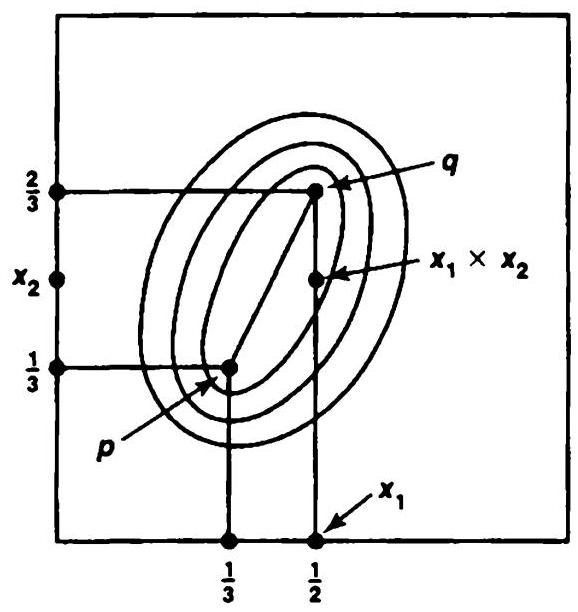
\includegraphics[width=0.5\textwidth]{images/37.1.jpg}
\end{center}
\hspace*{3em} 

Figure 37.1

``Aha!'' you say,''you made a bad choice. If after choosing \({x}_{1} = \frac{1}{2}\) you had chosen \({x}_{2} = \frac{2}{3}\) , then you would have found a point in \(\mathop{\bigcap }\limits_{{A \in  \mathcal{A}}}A\) .'' The difficulty with our tentative proof is that it gave us too much freedom in picking \({x}_{1}\) and \({x}_{2}\) ; it allowed us to make a ``bad'' choice instead of a ``good'' choice.

How can we alter the proof so as to avoid this difficulty?

This question leads to the second idea of the proof: Perhaps if we expand the collection \(\mathcal{A}\) (retaining the finite intersection property, of course), that expansion will restrict the choices of \({x}_{1}\) and \({x}_{2}\) sufficiently that we will be forced to make the ``right'' choice. To illustrate, suppose that in the previous example we expand the collection \(\mathcal{A}\) to the collection \(\mathcal{D}\) consisting of all closed elliptical regions bounded by ellipses that have \(p = ( {\frac{1}{3},\frac{1}{3}})\) as one focus and any point of the line segment \({pq}\) as the other focus. This collection is illustrated in Figure 37.2. The new collection \(\mathcal{D}\) still has the finite intersection property. But if you try to choose a point \({x}_{1}\) in

\[
\mathop{\bigcap }\limits_{{D \in  \mathcal{D}}}\overline{{\pi }_{1}( D) }
\]

the only possible choice for \({x}_{1}\) is \(\frac{1}{3}\) Similarly, the only possible choice for \({x}_{2}\) is \(\frac{1}{3}\) . And \(\frac{1}{3} \times  \frac{1}{3}\) does belong to every set \(D\) , and hence to every set \(A\) . In other words, expanding the collection \(\mathcal{A}\) to the collection \(\mathcal{D}\) forces the proper choice on us.

\begin{center}
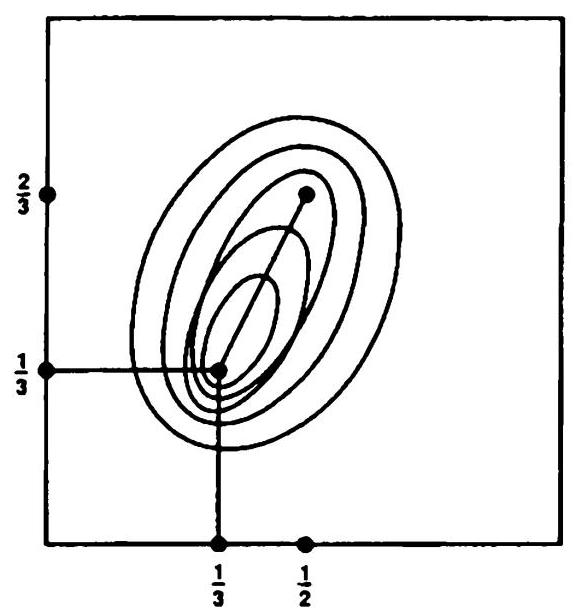
\includegraphics[width=0.5\textwidth]{images/37.2.jpg}
\end{center}
\hspace*{3em} 

Figure 37.2

Now of course in this example we chose \(\mathcal{D}\) carefully so that the proof would work. What hope can we have for choosing \(\mathcal{D}\) correctly in general? Here is the third idea of the proof: Why not simply choose \(\mathcal{D}\) to be a collection that is ``as large as possible''- so that no larger collection has the finite intersection property—and see whether such a \(\mathcal{D}\) will work? It is not at all obvious that such a collection \(\mathcal{D}\) exists; to prove it, we must appeal to Zorn's lemma. But after we prove that \(\mathcal{D}\) exists, we shall in fact be able to show that \(\mathcal{D}\) is large enough to force the proper choices on us.

A final remark. The assumption that the elements of the collection \(\mathcal{A}\) were closed sets was irrelevant in this discussion. For even if the set \(A \in  \mathcal{A}\) is closed, the set \({\pi }_{1}( A)\) need not be closed, so we had to take its closure in order to apply the closed set formulation of compactness. Therefore, we may as well begin with an arbitrary collection of subsets of \(X\) having the finite intersection property, and prove that the intersection of their closures is nonempty. This approach actually proves to be more convenient.

\begin{lemma}
	Let \(X\) be a set; let \(\mathcal{A}\) be a collection of subsets of \(X\) having the finite intersection property. Then there is a collection \(\mathcal{D}\) of subsets of \(X\) such that \(\mathcal{D}\) contains \(\mathcal{A}\) , and \(\mathcal{D}\) has the finite intersection property, and no collection of subsets of \(X\) that properly contains \(\mathcal{D}\) has this property.
\end{lemma}

We often say that a collection \(\mathcal{D}\) satisfying the conclusion of this theorem is maximal with respect to the finite intersection property

\begin{proof}
	As you might expect, we construct \(\mathcal{D}\) by using Zorn's lemma. It states that, given a set \(A\) that is strictly partially ordered, in which every simply ordered subset has an upper bound, \(A\) itself has a maximal element.
The set \(A\) to which we shall apply Zorn's lemma is not a subset of \(X\) , nor even a collection of subsets of \(X\) , but a set whose elements are collections of subsets of \(X\) . For purposes of this proof, we shall call a set whose elements are collections of subsets of \(X\) a ``\index{superset}'' and shall denote it by an outline letter. To summarize the rotation:

\(c\) is an element of \(X\) .

\(C\) is a subset of \(X\)

\(C\) is a collection of subsets of \(X\)

\(\mathbb{C}\) is a \index{Superset}\index{Superset}\index{superset@Superset}\index{superset@Superset}superset whose elements are collections of subsets of \(X\) .

Now by hypothesis, we have a collection \(\mathcal{A}\) of subsets of \(X\) that has the finite intersection property. Let \(\mathbf{A}\) denote the superset consisting of all collections \(\mathcal{B}\) of subsets of \(X\) such that \(\mathcal{B} \supset  \mathcal{A}\) and \(\mathcal{B}\) has the finite intersection property. We use proper inclusion \(\subsetneq\) as our strict partial order on \(\mathbf{A}\) . To prove our lemma, we need to show that \(\mathbf{A}\) has a maximal element \(\mathcal{D}\) .

In order to apply Zorn's lemma, we must show that if \(\mathbb{B}\) is a ``subsuperset'' of \(\mathbf{A}\) that is simply ordered by proper inclusion, then \(\mathbb{B}\) has an upper bound in \(\mathbb{A}\) . We shall show in fact that the collection

\[
\mathcal{C} = \mathop{\bigcup }\limits_{{\mathcal{B} \in  \mathbb{B}}}\mathcal{B}
\]

which is the union of the collections belongingg to \(\mathbb{B}\) , is an element of \(\mathbb{A}\) , then it is the required upper bound on \(\mathbb{B}\) .

To show that \(\mathcal{C}\) is an element of \(\mathbf{A}\) , we must show that \(\mathcal{C} \supset  \mathcal{A}\) and that \(\mathcal{C}\) has the finite intersection property. Certainly \(\mathcal{C}\) contains \(\mathcal{A}\) , since each element of \(\mathcal{B}\) contains \(\mathcal{A}\) . To show that \(\mathcal{C}\) has the finite intersection property, let \({C}_{1},\ldots ,{C}_{n}\) be elements, of \(\mathcal{C}\) . Because \(\mathcal{C}\) is the union of the elements of \(\mathbb{B}\) , there is, for each \(i\) , an element \({\mathcal{B}}_{i}\) of \(\mathbb{B}\) such that \({C}_{i} \in  {\mathcal{B}}_{i}\) . The superset \(\{  {{\mathcal{B}}_{1},\ldots ,{\mathcal{B}}_{n}}\}\) is contained in \(\mathbb{B}\) , so it is simply ordered by the relation of proper inclusion. Being finite, it has a largest element; that is, there is an index \(k\) such that \({\mathcal{B}}_{i} \subset  {\mathcal{B}}_{k}\) for \(i = 1,\ldots ,n\) . Then all the sets \({C}_{1},\ldots ,{C}_{n}\) are elements of \({\mathcal{B}}_{k}\) . Since \({\mathcal{B}}_{k}\) has the finite intersection property, the intersection of the sets \({C}_{1},\ldots ,{C}_{n}\) is nonempty, as desired.
\end{proof}
\begin{lemma}
	Let \(X\) be a set; let \(\mathcal{D}\) be a collection of subsets of \(X\) that is maximal with respect to the finite intersection property. Then:

(a) Any finite intersection of elements of \(\mathcal{D}\) is an element of \(\mathcal{D}\) .

(b) If \(A\) is a subset of \(X\) that intersects every element of \(\mathcal{D}\) , then \(A\) is an element of \(\mathcal{D}\) .
\end{lemma}

\begin{proof}
	(a) Let \(B\) equal the intersection of finitely many elements of \(\mathcal{D}\) . Define a collection \(\mathcal{E}\) by adjoining \(B\) to \(\mathcal{D}\) , so that \(\mathcal{E} = \mathcal{D} \cup  \{ B\}\) . We show that \(\mathcal{E}\) has the finite intersection property; then maximality of \(\mathcal{D}\) implies that \(\mathcal{E} = \mathcal{D}\) , so that \(B \in  \mathcal{D}\) as desired
Take finitely many elements of \(\mathcal{E}\) . If none of them is the set \(B\) , then their intersection is nonempty because \(\mathcal{D}\) has the finite intersection property. If one of them is the set \(B\) , then their intersection is of the form

\[
{D}_{1} \cap   \cdot   \cdot   \cap  {D}_{m} \cap  B
\]

Since \(B\) equals a finite intersection of elements of \(\mathcal{D}\) , this set is nonempty.

(b) Given \(A\) , define \(\mathcal{E} = \mathcal{D} \cup  \{ A\}\) We show that \(\mathcal{E}\) has the finite intersection property, from which we conclude that \(A\) belongs to \(\mathcal{D}\) . Take finitely many elements of \(\mathcal{E}\) . If none of them is the set \(A\) , their intersection is automatically nonempty. Otherwise, it is of the form

\[
{D}_{1} \cap  \cdots  \cap  {D}_{n} \cap  A\text{ . }
\]

Now \({D}_{1} \cap  \cdots  \cap  {D}_{n}\) belongs to \(\mathcal{D}\) , by (a); therefore, this intersection is nonempty, by hypothesis.
\end{proof}
\begin{theorem}[Tychon\index{Compactness!of product space}\index{Compactness!of product space}off theorem]
	An arbitrary product of compact spaces is compact in the product topology
\end{theorem}

\begin{proof}
	Let
\[
X = \mathop{\prod }\limits_{{\alpha  \in  J}}{X}_{\alpha }
\]

where each space \({X}_{\alpha }\) is compact. Let \(\mathcal{A}\) be a collection of subsets of \(X\) having the finite intersection property. We prove that the intersection

\[
\mathop{\bigcap }\limits_{{A \in  A}}\bar{A}
\]

is nonempty. Compactness of \(X\) follows.

Applying Lemma 37.1, choose a collection \(\mathcal{D}\) of subsets of \(X\) such that \(\mathcal{D} \supset  \mathcal{A}\) and \(\mathcal{D}\) is maximal with respect to the finite intersection property It will suffice to show that the intersection \(\mathop{\bigcap }\limits_{{D \in  \mathcal{D}}}\bar{D}\) is nonempty.

Given \(\alpha  \in  J\) , let \({\pi }_{\alpha } : X \rightarrow  {X}_{\alpha }\) be the projection map, as usual Consider the collection

\[
\{  {{\pi }_{\alpha }( D)  \mid  D \in  \mathcal{D}}\}
\]

of subsets of \({X}_{\alpha }\) . This collection has the finite intersection property because \(\mathcal{D}\) does. By compactness of \({X}_{\alpha }\) , we can for each \(\alpha\) choose a point \({x}_{\alpha }\) of \({X}_{\alpha }\) such that

\[
{x}_{\alpha } \in  \mathop{\bigcap }\limits_{{D \in  \mathcal{D}}}\overline{{\pi }_{\alpha }( D) }.
\]

Let \(\mathbf{x}\) be the point \({( {x}_{\alpha }) }_{\alpha  \in  J}\) of \(X\) . We shall show that \(\mathbf{x} \in  \bar{D}\) for every \(D \in  \mathcal{D}\) ; then our proof will be finished.

First we show that if \({\pi }_{\beta }^{-1}( {U}_{\beta })\) is any subbasis element (for the product topology on \(X\) ) containing \(\mathbf{x}\) , then \({\pi }_{\beta }^{-1}( {U}_{\beta })\) intersects every element of \(\mathcal{D}\) . The set \({U}_{\beta }\) is a neighborhood of \({x}_{\beta }\) in \({X}_{\beta }\) . Since \({x}_{\beta } \in  \overline{{\pi }_{\beta }( D) }\) by definition, \({U}_{\beta }\) intersects \({\pi }_{\beta }( D)\) in some point \({\pi }_{\beta }( \mathbf{y})\) , where \(\mathbf{y} \in  D\) Then it follows that \(\mathbf{y} \in  {\pi }_{\beta }^{-1}( {U}_{\beta })  \cap  D\) .

It follows from (b) of Lemma 37.2 that every subbasis element containing \(\mathbf{x}\) belongs to \(\mathcal{D}\) . And then it follows from (a) of the same lemma that every basis element containing \(\mathbf{x}\) belongs to \(\mathcal{D}\) . Since \(\mathcal{D}\) has the finite intersection property, this means that every basis element containing \(\mathbf{x}\) intersects every element of \(\mathcal{D}\) ; hence \(\mathbf{x} \in  \bar{D}\) for every \(D \in  \mathcal{D}\) as desired.
\end{proof}
\section*{Exercises}
\begin{enumerate}[itemsep=0.4em, parsep=0pt, topsep=0pt, partopsep=0pt, leftmargin=*, label=\arabic*., ref=\arabic*]
\item Let \(X\) be a space. Let \(\mathcal{D}\) be a collection of subsets of \(X\) that is maximal with respect to the finite intersection property
  \begin{enumerate}[itemsep=0.2em, parsep=0pt, topsep=0pt, partopsep=0pt, leftmargin=*, label=(\alph*), align=left]
  \item Show that \(x \in  \bar{D}\) for every \(D \in  \mathcal{D}\) if and only if every neighborhood of \(x\) belongs to \(\mathcal{D}\) . Which implication uses maximality of \(\mathcal{D}\) ?
  \item Let \(D \in  \mathcal{D}\) . Show that if \(A \supset  D\) , then \(A \in  \mathcal{D}\) .
  \item Show that if \(X\) satisfies the \({T}_{1}\) axiom, there is at most one point belongingg to \(\mathop{\bigcap }\limits_{{D \in  \mathcal{D}}}\bar{D}\) .
  \end{enumerate}
\item A collection \(\mathcal{A}\) of subsets of \(X\) has the \index{countable intersection property} if every countable intersection of elements of \(\mathcal{A}\) is nonempty. Show that \(X\) is a Lindelöf space if and only if for every collection \(\mathcal{A}\) of subsets of \(X\) having the \index{Countable intersection property}\index{Countable intersection property}\index{countable intersection property@Countable intersection property}\index{countable intersection property@Countable intersection property}countable intersection property,
\end{enumerate}
\section*{\(\mathop{\bigcap }\limits_{{A \in  A}}\bar{A}\)}

is nonempty.

3. Consider the three statements:

(i) If \(X\) is a set and \(\mathcal{A}\) is a collection of subsets of \(X\) having the countable intersection property, then there is a collection \(\mathcal{D}\) of subsets of \(X\) such that \(\mathcal{D} \supset  \mathcal{A}\) and \(\mathcal{D}\) is maximal with respect to the countable intersection property

(ii) Suppose \(\mathcal{D}\) is maximal with respect to the countable intersection property Then countable intersections of elements of \(\mathcal{D}\) are in \(\mathcal{D}\) . Furthermore, if \(A\) is a subset of \(X\) that intersects every element of \(\mathcal{D}\) , then \(A\) is an element of \(\mathcal{D}\) .

(iii) Products of Lindelöf spaces are Lindelöf.

(a) Show that (i) and (ii) together imply (iii).

(b) Show that (ii) holds.

(c) Products of Lindelöf spaces need not be Lindelöf (see §30). Therefore (i) does not hold. If one attempts to generalize the proof of Lemma 37.1 to the countable intersection property, at what point does the proof break down?

4. Here is another theorem whose proof uses Zorn's lemma. Recall that if \(A\) is a space and if \(x,y \in  A\) , we say that \(x\) and \(y\) belong to the same quasicomponent of \(A\) if there is no separation \(A = C \cup  D\) of \(A\) into two disjoint sets open in \(A\) such that \(x \in  C\) and \(y \in  D\) .

\begin{theorem}
	Let \(X\) be a compact Hausdorff space. Then \(x\) and \(y\) belong to the same quasicomponent of \(X\) if and only if they belong to the same component of \(X\) .
\end{theorem}

(a) Let \(A\) be the collection of all closed subspaces \(A\) of \(X\) such that \(x\) and \(y\) lie in the same quasicomponent of \(A\) . Let \(\mathcal{B}\) be a subcollection of \(\mathcal{A}\) that is simply ordered by proper inclusion. Show that the intersection of the elements of \(\mathcal{B}\) belongs to \(\mathcal{A}\) . [Hint: Compare Exercise 11 of §26.]

(b) Show \(\mathcal{A}\) has a minimal element \(D\) .

(c) Show \(D\) is connected.

*5. Here is a proof of the Tychonoff theorem that relies on the well-ordering theorem rather than on Zorn's lemma. First, prove the following version of the tube lemma; then prove the theorem.

\begin{lemma}
	Let \(\mathcal{A}\) be a collection of basis elements for the topology of the product space \(X \times  Y\) , such that no finite subcollection of \(\mathcal{A}\) covers \(X \times  Y\) . If \(X\) is compact, there is a point \(x \in  X\) such that no finite subcollection of \(\mathcal{A}\) covers the slice \(\{ x\}  \times  Y\) .
\end{lemma}

\begin{theorem}
	An arbitrary product of compact spaces is compact in the product topology.
\end{theorem}

\begin{proof}
	Let \({\{  {X}_{\alpha }\}  }_{\alpha  \in  J}\) be an indexed family of compact spaces, let
\[
X = \mathop{\prod }\limits_{{\alpha  \in  J}}{X}_{\alpha }
\]

Let \({\pi }_{\alpha } : X \rightarrow  {X}_{\alpha }\) be the projection map. Well-order \(J\) , once and for all, in such a way that \(J\) has a largest element.

(a) Let \(\beta  \in  J\) Suppose points \({p}_{i} \in  {X}_{i}\) are given, for all \(i < \beta\) . For any \(\alpha  < \beta\) , let \({Y}_{\alpha }\) denote the subspace of \(X\) defined by the equation

\[
{Y}_{\alpha } = \{  {\mathbf{x} \mid  {\pi }_{i}( \mathbf{x})  = {p}_{i}\text{ for }i \leq  \alpha }\}  .
\]

Note that if \(\alpha  < {\alpha }^{\prime }\) , then \({Y}_{\alpha } \supset  {Y}_{{\alpha }^{\prime }}\) . Show that if \(\mathcal{A}\) is a finite collection of

basis elements for \(X\) that covers the space

\[
{Z}_{\beta } = \mathop{\bigcap }\limits_{{\alpha  < \beta }}{Y}_{\alpha } = \{  {\mathbf{x} \mid  {\pi }_{i}( \mathbf{x})  = {p}_{i}\text{ for }i < \beta }\}
\]

then \(\mathcal{A}\) actually covers \({Y}_{\alpha }\) for some \(\alpha  < \beta\) . [Hint. If \(\beta\) has an immediate predecessor in \(J\) , let \(\alpha\) be that immediate predecessor Otherwise, for each \(A \in  \mathcal{A}\) , let \({J}_{A}\) denote the set of those indices \(i < \beta\) for which \({\pi }_{i}( A)  \neq  {X}_{i}\) ; the union of the sets \({J}_{A}\) , for \(A \in  \mathcal{A}\) , is finite; let \(\alpha\) be the largest element of this union.]

(b) Assume \(\mathcal{A}\) is a collection of basis elements for \(X\) such that no finite subcol-lection of \(\mathcal{A}\) covers \(X\) . Show that one can choose points \({p}_{i} \in  {X}_{i}\) for all \(i\) , such that for each \(\alpha\) , the space \({Y}_{\alpha }\) defined in (a) cannot be finitely covered by \(\mathcal{A}\) . When \(\alpha\) is the largest element of \(J\) , one has a contradiction. [Hint: If \(\alpha\) is the smallest element of \(J\) , use the preceding lemma to choose \({p}_{\alpha }\) . If \({p}_{i}\) is defined for all \(i < \beta\) , note that (a) implies that the space \({Z}_{\beta }\) cannot be finitely covered by \(\mathcal{A}\) and use the lemma to find \({p}_{\beta }\) ]
\end{proof}
\section*{§ 38 The Stone-Čech Compactification}

We have already studied one way of compactifying a topological space \(X\) , the one-point compactification (§29); it is in some sense the minimal compactification of \(X\) . The Stone-Čech compactification of \(X\) , which we study now, is in some sense the maximal compactification of \(X\) . It was constructed by M. Stone and E. Čech, independently, in 1937 It has a number of applications in modern analysis, but these lie outside the scope of this book

We recall the following definition

\begin{definition}
	A compactification of a space \(X\) is a compact Hausdorff space \(Y\) containing \(X\) as a subspace such that \(\bar{X} = Y\) . Two compactifications \({Y}_{1}\) and \({Y}_{2}\) of \(X\) are said to be equivalent if there is a homeomorphism \(h : {Y}_{1} \rightarrow  {Y}_{2}\) such that \(h( x)  = x\) for every \(x \in  X\) .
\end{definition}

If \(X\) has a compactification \(Y\) , then \(X\) must be completely regular, being a subspace of the completely regular space \(Y\) . Conversely, if \(X\) is completely regular, then \(X\) has a compactification. For \(X\) can be imbedded in the compact Hausdorff space \({[  0,1]  }^{J}\) for some \(J\) , and any such imbedding gives rise to a compactification of \(X\) , as the following lemma shows

\begin{lemma}
	Let \(X\) be a space; suppose that \(h : X \rightarrow  Z\) is an imbedding of \(X\) in the compact Hausdorff space \(Z\) . Then there exists a corresponding compactification \(Y\) of \(X\) ; it has the property that there is an imbedding \(H : Y \rightarrow  Z\) that equals \(h\) on \(X\) . The compactification \(Y\) is uniquely determined up to \index{Equivalence of compactifications} equivalence.
\end{lemma}

We call \(Y\) the compactification induced by the imbedding \(h\) .

\begin{proof}
	Given \(h\) , let \({X}_{0}\) denote the subspace \(h( X)\) of \(Z\) , and let \({Y}_{0}\) denote its closure in \(Z\) . Then \({Y}_{0}\) is a compact Hausdorff space and \({\bar{X}}_{0} = {Y}_{0}\) ; therefore, \({Y}_{0}\) is a compactification of \({X}_{0}\) .
We now construct a space \(Y\) containing \(X\) such that the pair(X, Y)is homeomorphic to the pair \(( {{X}_{0},{Y}_{0}})\) . Let us choose a set \(A\) disjoint from \(X\) that is in bijective correspondence with the set \({Y}_{0} - {X}_{0}\) under some map \(k : A \rightarrow  {Y}_{0} - {X}_{0}\) . Define \(Y = X \cup  A\) , and define a bijective correspondence \(H : Y \rightarrow  {Y}_{0}\) by the rule

\[
H( x)  = h( x) \;\text{ for }x \in  X,
\]

\[
H( a)  = k( a) \;\text{ for }a \in  A.
\]

Then topologize \(Y\) by declaring \(U\) to be open in \(Y\) if and only if \(H( U)\) is open in \({Y}_{0}\) . The map \(H\) is automatically a homeomorphism; and the space \(X\) is a subspace of \(Y\) because \(H\) equals the homeomorphism \(h\) when restricted to the subspace \(X\) of \(Y\) . By expanding the range of \(H\) , we obtain the required imbedding of \(Y\) into \(Z\) .

Now suppose \({Y}_{i}\) is a compactification of \(X\) and that \({H}_{i} : {Y}_{i} \rightarrow  Z\) is an imbedding that is an extension of \(h\) , for \(i = 1,2\) . Now \({H}_{i}\) maps \(X\) onto \(h( X)  = {X}_{0}\) Because \({H}_{t}\) is continuous, it must map \({Y}_{t}\) into \({\bar{X}}_{0}\) ; because \({H}_{i}( {Y}_{i})\) contains \({X}_{0}\) and is closed (being compact), it contains \({\bar{X}}_{0}\) . Hence \({H}_{i}( {Y}_{i})  = {\bar{X}}_{0}\) , and \({H}_{2}^{-1} \circ  {H}_{1}\) defines a homeomorphism of \({Y}_{1}\) with \({Y}_{2}\) that equals the identity on \(X\) .

In general, there are many different ways of compactifying a given space \(X\) . Consider for instance the following compactifications of the open interval \(X = ( {0,1})\) :

\begin{centeredblock}
\begin{example}
	Take the unit circle \({S}^{1}\) in \({\mathbb{R}}^{2}\) and let \(h.( {0,1})  \rightarrow  {S}^{1}\) be the map

\[
h( \iota )  = ( {\cos {2\pi \iota }})  \times  ( {\sin {2\pi \iota }}) .
\]

The compactification induced by the imbedding \(h\) is equivalent to the one-point compactification of \(X\)
\end{example}
\end{centeredblock}

\begin{centeredblock}
\begin{example}
	Let \(Y\) be the space \([  {0,1}]\) Then \(Y\) is a compacufication of \(X\) , it is obtained by ``adding one point at each end of(0,1)''
\end{example}
\end{centeredblock}

\begin{centeredblock}
\begin{example}
	Consider the square \({[  -1,1]  }^{2}\) in \({\mathbb{R}}^{2}\) and let \(h\;( {0,1})  \rightarrow  {[  -1,1]  }^{2}\) be the map

\[
h( x)  = x \times  \sin ( {1/x}) .
\]

The space \({Y}_{0} = \overline{h( X) }\) is the topologist's sine curve (see Example 7 of §24). The imbedding \(h\) gives rise to a compactification of(0,1)quite different from the other two. It is obtained by adding one point at the right-hand end of(0,1), and an entire line segment of points at the left-hand end \({}^{1}\)
\end{example}
\end{centeredblock}

A basic problem that occurs in studying compactifications is the following:

If \(Y\) is a compactification of \(X\) , under what conditions can a continuous real-valued function \(f\) defined on \(X\) be extended continuously to \(Y\) ? The function \(f\) will have to be bounded if it is to be extendable, since its extension will carry the compact space \(Y\) into \(\mathbb{R}\) and will thus be bounded. But boundedness is not enough, in general. Consider the following example

\begin{centeredblock}
\begin{example}
	Let \(X = ( {0,1})\) Consider the one-point compactification of \(X\) given in Example I A bounded continuous function \(f : ( {0,1})  \rightarrow  \mathbb{R}\) is extendable to this compacutfication if and only if the limits

\[
\mathop{\lim }\limits_{{x \rightarrow  0 + }}f( x) \;\text{ and }\;\mathop{\lim }\limits_{{x \rightarrow  1 - }}f( x)
\]

exist and are equal.
\end{example}
\end{centeredblock}

For the ``the two-point compactification'' of \(X\) considered in Example 2, the function \(f\) is extendable if and only if both these limits simply exist

For the compactification of Example 3, extensions exist for a still broader class of functions It is easy to see that \(f\) is extendable if both the above limits exist But the function \(f( x)  = \sin ( {1/x})\) is also extendable to this compactification. Let \(H\) be the imbedding of \(Y\) in \({\mathbb{R}}^{2}\) that equals \(h\) on the subspace \(X\) Then the composite map

\[
Y\overset{H}{ \rightarrow  }\mathbb{R} \times  \mathbb{R}\overset{{\pi }_{2}}{ \rightarrow  }\mathbb{R}
\]

is the desired extension of \(f\) . For if \(x \in  X\) , then \(H( x)  = h( x)  = x \times  \sin ( {1/x})\) , so that \({\pi }_{2}( {H( x) })  = \sin ( {1/x})\) , as desired

There is something especially interesting about this last compactification. We constructed it by choosing an imbedding

\[
h.( {0,1})  \rightarrow  {\mathbb{R}}^{2}
\]

whose component functions were the functions \(x\) and \(\sin ( {1/x})\) Then we found that both the functions \(x\) and \(\sin ( {1/x})\) could be extended to the compactification This suggests that if we have a whole collection of bounded continuous functions defined on(0,1), we might use them as component functions of an imbedding of(0,1)into \({\mathbb{R}}^{J}\) for some \(J\) , and thereby obtain a compactification for which every function in the collection is extendable.

This idea is the basic idea behind the Stone-Čech compactification. It is defined as follows:
\end{proof}
\begin{theorem}
	Let \(X\) be a completely regular space. There exists a compactification \(Y\) of \(X\) having the property that every bounded continuous map \(f : X \rightarrow  \mathbb{R}\) extends uniquely to a continuous map of \(Y\) into \(\mathbb{R}\) .
\end{theorem}

\begin{proof}
	Let \({\{  {f}_{\alpha }\}  }_{\alpha  \in  J}\) be the collection of all bounded continuous real-valued functions on \(X\) , indexed by some index set \(J\) For each \(\alpha  \in  J\) , choose a closed interval \({I}_{\alpha }\) in \(\mathbb{R}\) containing \({f}_{\alpha }( X)\) . To be definite, choose
\[
{I}_{\alpha } = \{  {\inf {f}_{\alpha }( X) ,\sup {f}_{\alpha }( X) }\}  .
\]

Then define \(h : X \rightarrow  \mathop{\prod }\limits_{{\alpha  \in  J}}{I}_{\alpha }\) by the rule

\[
h( x)  = {( {f}_{\alpha }( x) ) }_{\alpha  \in  J}.
\]

By the Tychonoff theorem, \(\prod {I}_{\alpha }\) is compact Because \(X\) is completely regular, the collection \(\{  {f}_{\alpha }\}\) separates points from closed sets in \(X\) . Therefore, by Theorem 34.2, the map \(h\) is an imbedding.

Let \(Y\) be the compactification of \(X\) \index{Compactification!induced by an imbedding}\index{Compactification!induced by an imbedding}induced by the imbedding \(h\) . Then there is an imbedding \(H : Y \rightarrow  \prod {I}_{\alpha }\) that equals \(h\) when restricted to the subspace \(X\) of \(Y\) . Given a bounded continuous real-valued function \(f\) on \(X\) , we show it extends to \(Y\) . The function \(f\) belongs to the collection \({\{  {f}_{\alpha }\}  }_{\alpha  \in  J}\) , so it equals \({f}_{\beta }\) for some index \(\beta\) . Let \({\pi }_{\beta }.\prod {I}_{\alpha } \rightarrow  {I}_{\beta }\) be the projection mapping Then the continuous map \({\pi }_{\beta } \circ  H\) : \(Y \rightarrow  {I}_{\beta }\) is the desired extension of \(f\) . For if \(x \in  X\) , we have

\[
{\pi }_{\beta }( {H( x) })  = {\pi }_{\beta }( {h( x) })  = {\pi }_{\beta }( {( {f}_{\alpha }( x) ) }_{\alpha  \in  J})  = {f}_{\beta }( x) .
\]

\index{Stone-Čech compactification!uniqueness}\index{Stone-Čech compactification!uniqueness}\index{Stone-Čech compactification!uniqueness}\index{Stone-Čech compactification!uniqueness}Uniqueness of the extension is a consequence of the following lemma.
\end{proof}
\begin{lemma}
	Let \(A \subset  X\) ; let \(f : A \rightarrow  Z\) be a continuous map of \(A\) into the Hausdorff space \(Z\) . There is at most one extension of \(f\) to a continuous function \(g : \bar{A} \rightarrow  Z\) .
\end{lemma}

\begin{proof}
	This lemma was given as an exercise in \(\$ {18}\) ; we give a proof here. Suppose that \(g,{g}^{\prime } \cdot  \bar{A} \rightarrow  X\) are two different extensions of \(f\) , choose \(x\) so that \(g( x)  \neq  {g}^{\prime }( x)\) . Let \(U\) and \({U}^{\prime }\) be disjoint neighborhoods of \(g( x)\) and \({g}^{\prime }( x)\) , respectively. Choose a neighborhood \(V\) of \(x\) so that \(g( V)  \subset  U\) and \({g}^{\prime }( V)  \subset  {U}^{\prime }\) Now \(V\) intersects \(A\) in some point \(y\) ; then \(g( y)  \in  U\) and \({g}^{\prime }( y)  \in  {U}^{\prime }\) . But since \(y \in  A\) , we have \(g( y)  = f( y)\) and \({g}^{\prime }( y)  = f( y)\) . This contradicts the fact that \(U\) and \({U}^{\prime }\) are disjoint.
\end{proof}
\begin{theorem}
	Let \(X\) be a completely regular space; let \(Y\) be a compactification of \(X\) satisfying the extension property of Theorem 38.2 Given any continuous map \(f : X \rightarrow  C\) of \(X\) into a compact Hausdorff space \(C\) , the map \(f\) extends uniquely to a continuous map \(g : Y \rightarrow  C\) .
\end{theorem}

\begin{proof}
	Note that \(C\) is completely regular, so that it can be imbedded in \({[  0,1]  }^{J}\) for some \(J\) So we may as well assume that \(C \subset  \{ 0,1{\} }^{J}\) . Then each component function \({f}_{\alpha }\) of the map \(f\) is a bounded continuous real-valued function on \(X\) , by hypothesis, \({f}_{\alpha }\) can be extended to a continuous map \({g}_{\alpha }\) of \(Y\) into \(\mathbb{R}\) . Define \(g : Y \rightarrow  {\mathbb{R}}^{J}\) by setting \(g( y)  = {( {g}_{\alpha }( y) ) }_{\alpha  \in  J}\) ; then \(g\) is continuous because \({\mathbb{R}}^{J}\) has the product topology. Now in fact \(g\) maps \(Y\) into the subspace \(C\) of \({\mathbb{R}}^{J}\) . For continuity of \(g\) implies that
\[
g( Y)  = g( \bar{X})  \subset  \overline{g( X) } = \overline{f( X) } \subset  \bar{C} = C.
\]

Thus \(g\) is the desired extension of \(f\)
\end{proof}
\begin{theorem}
	Let \(X\) be a completely regular space. If \({Y}_{1}\) and \({Y}_{2}\) are two compact-ifications of \(X\) satisfying the extension property of Theorem 38.2, then \({Y}_{1}\) and \({Y}_{2}\) are equivalent.
\end{theorem}

\begin{proof}
	Consider the inclusion mapping \({j}_{2} : X \rightarrow  {Y}_{2}\) . It is a continuous map of \(X\) into the compact Hausdorff space \({Y}_{2}\) . Because \({Y}_{1}\) has the extension property, we may, by the preceding theorem, extend \({j}_{2}\) to a continuous map \({f}_{2} : {Y}_{1} \rightarrow  {Y}_{2}\) . Similarly, we may extend the inclusion map \({j}_{1} : X \rightarrow  {Y}_{1}\) to a continuous map \({f}_{1} : {Y}_{2} \rightarrow  {Y}_{1}\) (because \({Y}_{2}\) has the extension property and \({Y}_{1}\) is compact Hausdorff).
\begin{center}
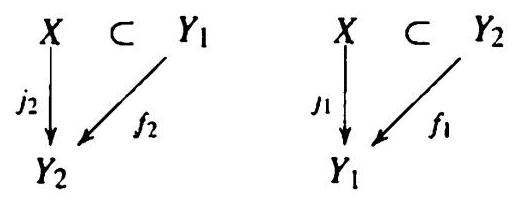
\includegraphics[width=0.4\textwidth]{images/37.3.jpg}
\end{center}
\hspace*{3em} 

The composite \({f}_{1} \circ  {f}_{2} : {Y}_{1} \rightarrow  {Y}_{1}\) has the property that for every \(x \in  X\) , one has \({f}_{1}( {{f}_{2}( x) })  = x\) Therefore, \({f}_{1} \circ  {f}_{2}\) is a continuous extension of the identity map \({i}_{X} : X \rightarrow  X\) . But the identity map of \({Y}_{1}\) is also a continuous extension of \({i}_{X}\) . By uniqueness of extensions (Lemma 38.3), \({f}_{1} \circ  {f}_{2}\) must equal the identity map of \({Y}_{1}\) . Similarly, \({f}_{2} \circ  {f}_{1}\) must equal the identity map of \({Y}_{2}\) Thus \({f}_{1}\) and \({f}_{2}\) are homeomorphisms.
\end{proof}
\begin{definition}
	For each completely regular space \(X\) , let us choose, once and for all, a compactification of \(X\) satisfying the \index{Stone-Čech compactification!extension condition}\index{Stone-Čech compactification!extension condition}\index{Stone-Čech compactification!extension condition}\index{Stone-Čech compactification!extension condition}extension condition of Theorem 38.2. We will denote this compactification of \(X\) by \(\beta ( X)\) and call it the Stone-Čech compactification of \(X\) . It is characterized by the fact that any continuous map \(f : X \rightarrow  C\) of \(X\) into a compact Hausdorff space \(C\) extends uniquely to a continuous map \(g\;\beta ( X)  \rightarrow  C\) .
\end{definition}

\section*{Exercises}
\begin{enumerate}[itemsep=0.4em, parsep=0pt, topsep=0pt, partopsep=0pt, leftmargin=*, label=\arabic*., ref=\arabic*]
\item Verify the statements made in Example 4.
\item Show that the bounded continuous function \(g( {0,1})  \rightarrow  \mathbb{R}\) defined by \(g( x)  =\)  \(\cos ( {1/x})\) cannot be extended to the compactification of Example 3. Define an imbedding \(h : ( {0,1})  \rightarrow  {[  0,1]  }^{3}\) such that the functions \(x,\sin ( {1/x})\) , and \(\cos ( {1/x})\) are all extendable to the compactification induced by \(h\) .
\item Under what conditions does a metrizable space have a metrizable compactification?
\item Let \(Y\) be an arbitrary compactification of \(X\) ; let \(\beta ( X)\) be the Stone-Čech compactification. Show there is a continuous surjective closed map \(g : \beta ( X)  \rightarrow  Y\) that equals the identity on \(X\) [This exercise makes precise what we mean by saying that \(\beta ( X)\) is the ``maximal'' compactification of \(X\) . It shows that every compactification of \(X\) is equivalent to a quotient space of \(\beta ( X)\) .]
\item
  \begin{enumerate}[itemsep=0.2em, parsep=0pt, topsep=0pt, partopsep=0pt, leftmargin=*, label=(\alph*), align=left]
  \item Show that every continuous real-valued function defined on \({S}_{\Omega }\) is ``eventually constant.'' [Hint First prove that for each \(\epsilon\) , there is an element \(\alpha\) of \({S}_{\Omega }\) such that \(| {f( \beta )  - f( \alpha ) }|  < \epsilon\) for all \(\beta  > \alpha\) Then let \(\epsilon  = 1/n\) for \(n \in  {\mathbb{Z}}_{ + }\) and consider the corresponding points \(. {{\alpha }_{n}\text{ . }}]\)

  \item Show that the one-point compactification of \({S}_{\Omega }\) and the Stone-Čech compactification are equivalent.
  \item Conclude that every compactification of \({S}_{\Omega }\) is equivalent to the one-point compactification.
  \end{enumerate}
\item Let \(X\) be completely regular. Show that \(X\) is connected if and only if \(\beta ( X)\) is connected. [Hint: If \(X = A \cup  B\) is a separation of \(X\) , let \(f( x)  = 0\) for \(x \in  A\) and \(f( x)  = 1\) for \(x \in  B\) .]
\item Let \(X\) be a discrete space; consider the space \(\beta ( X)\) .
  \begin{enumerate}[itemsep=0.2em, parsep=0pt, topsep=0pt, partopsep=0pt, leftmargin=*, label=(\alph*), align=left]
  \item Show that if \(A \subset  X\) , then \(\bar{A}\) and \(\overline{X - A}\) are disjoint, where the closures are taken in \(\beta ( X)\) .
  \item Show that if \(U\) is open in \(\beta ( X)\) , then \(\bar{U}\) is open in \(\beta ( X)\) .
  \item Show that \(\beta ( X)\) is totally disconnected.
  \end{enumerate}
\item Show that \(\beta ( {\mathbb{Z}}_{ + })\) has cardinality at least as great as \({I}^{I}\) , where \(I = [  {0,1}]\) . [Hint: The space \({I}^{\prime }\) has a countable dense subset.]
\item
  \begin{enumerate}[itemsep=0.2em, parsep=0pt, topsep=0pt, partopsep=0pt, leftmargin=*, label=(\alph*), align=left]
  \item If \(X\) is normal and \(y\) is a point of \(\beta ( X)  - X\) , show that \(y\) is not the limit of a sequence of points of \(X\) .

  \item Show that if \(X\) is completely regular and noncompact, then \(\beta ( X)\) is not metrizable.
  \end{enumerate}
\item We have constructed a correspondence \(X \rightarrow  \beta ( X)\) that assigns, to each completely regular space, its Stone-Čech compactification. Now let us assign, to each continuous map \(f : X \rightarrow  Y\) of completely regular spaces, the unique continuous map \(\beta ( f)  : \beta ( X)  \rightarrow  \beta ( Y)\) that extends the map \(i \circ  f\) , where \(i : Y \rightarrow  \beta ( Y)\) is the inclusion map. Verify the following:
  \begin{enumerate}[itemsep=0.2em, parsep=0pt, topsep=0pt, partopsep=0pt, leftmargin=*, label=(\alph*), align=left]
  \item If \({1}_{X} : X \rightarrow  X\) is the identity map of \(X\) , then \(\beta ( {1}_{X})\) is the identity map of \(\beta ( X)\) . (ii) If \(f : X \rightarrow  Y\) and \(g : Y \rightarrow  Z\) , then \(\beta ( {g \circ  f})  = \beta ( g)  \circ  \beta ( f)\) . These properties tell us that the correspondence we have constructed is what is called a functor; it is a functor from the ``category'' of completely regular spaces and continuous maps of such spaces, to the ``category'' of compact Hausdorff spaces and continuous maps of such spaces. You will see these properties again in Part II of the book; they are fundamental in algebra and in algebraic topology.
  \end{enumerate}
\end{enumerate}
\chapter{Metrization Theorems and Paracompactness}

The Urysohn metrization theorem of Chapter 4 was the first step-a giant one-toward an answer to the question: When is a topological space metrizable? It gives conditions under which a space \(X\) is metrizable. that it be regular and have a countable basis. But mathematicians are never satisfied with a theorem if there is some hope of proving a stronger one. In the present case, one can hope to strengthen the theorem by finding conditions on \(X\) that are both necessary and sufficient for \(X\) to be metrizable, that is, conditions that are equivalent to metrizability.

We know that the regularity hypothesis in the Urysohn metrization theorem is a necessary one, but the countable basis condition is not. So the obvious thing to do is try to replace the countable basis condition by something weaker. Finding such condition is a delicate task. The condition has to be strong enough to imply metrizability, and yet weak enough that all metrizable spaces satisfy it. In a situation like this, discovering the right hypothesis is more than half the battle.

The condition that was eventually formulated, by J. Nagata and Y. Smurnov independently, involves a new notion, that of local finiteness. We say that a collection \(\mathcal{A}\) of subsets of a space \(X\) is locally finite if every point of \(X\) has a neighborhood that intersects only finitely many elements of \(\mathcal{A}\) .

Now one way of expressing the condition that the basis \(\mathcal{B}\) is countable is to say that \(\mathcal{B}\) can be expressed in the form

\[
\mathcal{B} = \mathop{\bigcup }\limits_{{n \in  {\mathbb{Z}}_{ + }}}{\mathcal{B}}_{n}
\]

where each collection \({\mathcal{B}}_{n}\) is finite. This is an awkward way of saying that \(\mathcal{B}\) is countable, but it suggests how to formulate a weaker version of it. The Nagata-Smirnov condition is to require that the basis \(\mathcal{B}\) can be expressed in the form

\[
\mathcal{B} = \mathop{\bigcup }\limits_{{n \in  {\mathbb{Z}}_{ + }}}{\mathcal{B}}_{n}
\]

where each collection \({\mathcal{B}}_{n}\) is locally finite. We say that such a collection \(\mathcal{B}\) is \idx{countably locally finite}. Surprisingly enough, this condition, along with regularity, is both necessary and sufficient for metrizability of \(X\) . This we shall we prove.

There is another concept in topology that involves the notion of local finiteness. It is a generalization of the concept of compactness called ``\idx{paracompactness}.'' Although of fairly recent origin, it has proved useful in many parts of mathematics. We introduce it here so that we can give another set of necessary and sufficient conditions for a space \(X\) to be metrizable. It turns out that \(X\) is metrizable if and only if it is both paracompact and locally metrizable. This we prove in §42.

Some of the sections of this chapter are independent of one another. The dependence among them is expressed in the following diagram.

\begin{center}
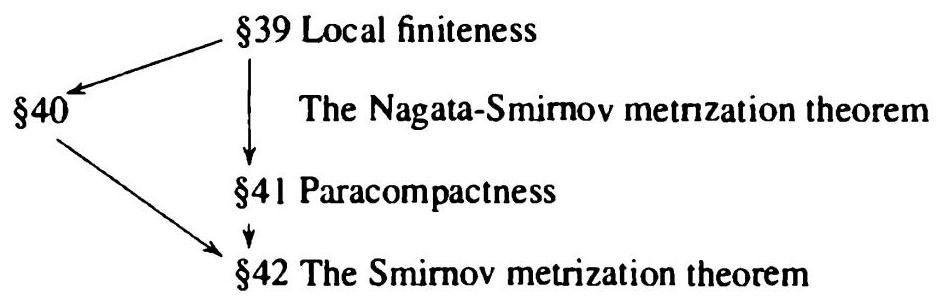
\includegraphics[width=0.8\textwidth]{images/38.1.jpg}
\end{center}
\hspace*{3em} 

\section*{§ 39 Local Finiteness}

In this sections we prove some elementary properties of \idx{locally finite collection}s and a crucial lemma about metrizable spaces.

\begin{definition}
	Let \(X\) be a topological space. A collection \(\mathcal{A}\) of subsets of \(X\) is said to be locally finite in \(X\) if every point of \(X\) has a neighborhood that intersects only finitely many elements of \(\mathcal{A}\)
\end{definition}

\begin{centeredblock}
\begin{example}
	The collection of intervals

\[
\mathcal{A} = \{ \left( {n,n + 2}\right)  \mid  n \in  \mathbb{Z}\}
\]

is locally finite in the topological space \(\mathbb{R}\) , as you can check. On the other hand, the collection

\[
\mathcal{B} = \left\{  {\left( {0,1/n}\right)  \mid  n \in  {\mathbb{Z}}_{ + }}\right\}
\]

is locally finite in(0,1)but not in \(\mathbb{R}\) , as is the collection

\[
\mathcal{C} = \left\{  {\left( {1/\left( {n + 1}\right) ,1/n}\right)  \mid  n \in  {\mathbb{Z}}_{ + }}\right\}
\]
\end{example}
\end{centeredblock}

\begin{lemma}
	Let \(\mathcal{A}\) be a locally finite collection of subsets of \(X\) . Then:

(a) Any subcollection of \(\mathcal{A}\) is locally finite.

(b) The collection \(\mathcal{B} = \{ \bar{A}{\} }_{A \in  \mathcal{A}}\) of the closures of the elements of \(\mathcal{A}\) is locally finite.

(c) \(\overline{\mathop{\bigcup }\limits_{{A \in  \mathcal{A}}}A} = \mathop{\bigcup }\limits_{{A \in  \mathcal{A}}}\overline{A}\) .
\end{lemma}

\begin{proof}
	Statement (a) is trivial. To prove (b), note that any open set \(U\) that intersects the set \(\bar{A}\) necessarily intersects \(A\) . Therefore, if \(U\) is a neighborhood of \(x\) that intersects only finitely many elements \(A\) of \(\mathcal{A}\) , then \(U\) can intersect at most the same number of sets of the collection \(\mathcal{B}\) . (It might intersect fewer sets of \(\mathcal{B}\) , since \({\bar{A}}_{1}\) and \({\bar{A}}_{2}\) can be equal even though \({A}_{1}\) and \({A}_{2}\) are not).
To prove (c), let \(Y\) denote the union of the elements of \(\mathcal{A}\) :

\[
\mathop{\bigcup }\limits_{{A \in  A}}A = Y
\]

In general, \(\bigcup \bar{A} \subset  \bar{Y}\) ; we prove the reverse inclusion, under the assumption of local finiteness. Let \(x \in  \bar{Y}\) ; let \(U\) be a neighborhood of \(x\) that intersects only finitely many elements of \(\mathcal{A}\) , say \({A}_{1},\ldots ,{A}_{k}\) . We assert that \(x\) belongs to one of the sets \({\bar{A}}_{1}\) , \(\ldots ,{\bar{A}}_{k}\) , and hence belongs to \(\bigcup \bar{A}\) . For otherwise, the set \(U - {\bar{A}}_{1} - \cdots  - {\bar{A}}_{k}\) would be a neighborhood of \(x\) that intersects no element of \(\mathcal{A}\) and hence does not intersect \(Y\) , contrary to the assumption that \(x \in  \bar{Y}\) .

There is an analogous concept of local finiteness for an indexed family of subsets of \(X\) . The indexed family \({\left\{  {A}_{\alpha }\right\}  }_{\alpha  \in  J}\) is said to be a locally finite indexed family in \(X\) if every \(x \in  X\) has a neighborhood that intersects \({A}_{\alpha }\) for only finitely many values of \(\alpha\) . What is the relation between the two formulations of local finiteness? It is easy to see that \({\left\{  {A}_{\alpha }\right\}  }_{\alpha  \in  J}\) is a locally finite indexed family if and only if it is locally finite as a collection of sets and each nonempty subset \(A\) of \(X\) equals \({A}_{\alpha }\) for at most finitely many values of \(\alpha\) .

We shall be concerned with locally finite indexed families only in §41, when we deal with partitions of unity.
\end{proof}
\begin{definition}
	A collection \(\mathcal{B}\) of subsets of \(X\) is said to be countably locally finite if \(\mathcal{B}\) can be written as the countable union of collections \({\mathcal{B}}_{n}\) , each of which is locally finite.
\end{definition}

Most authors use the term `` \(\sigma\) -locally finite'' for this concept. The \(\sigma\) comes from measure theory and stands for the phrase ``countable union of `` Note that both a countable collection and a locally finite collection are countably locally finite.

\begin{definition}
	Let \(\mathcal{A}\) be a collection of subsets of the space \(X\) . A collection \(\mathcal{B}\) of subsets of \(X\) is said to be a \idx{refinement} of \(\mathcal{A}\) (or is said to refine \(\mathcal{A}\) ) if for each element \(B\) of \(\mathcal{B}\) , there is an element \(A\) of \(\mathcal{A}\) containing \(B\) . If the elements of \(\mathcal{B}\) are open sets, we call \(\mathcal{B}\) an \idx{open refinement} of \(\mathcal{A}\) ; if they are closed sets, we call \(\mathcal{B}\) a \idx{closed refinement}
\end{definition}

\begin{lemma}
	Let \(X\) be a metrizable space. If \(\mathcal{A}\) is an open covering of \(X\) , then there is an open covering \(\mathcal{E}\) of \(X\) refining \(\mathcal{A}\) that is countably locally finite.
\end{lemma}

\begin{proof}
	We shall use the well-ordering theorem in proving this theorem. Choose a well-ordering \(<\) for the collection \(\mathcal{A}\) . Let us denote the elements of \(\mathcal{A}\) generically by the letters \(U,V,W,\ldots\) .
Choose a metric for \(X\) . Let \(n\) be a positive integer, fixed for the moment. Given an element \(U\) of \(\mathcal{A}\) , let us define \({S}_{n}\left( U\right)\) to be the subset of \(U\) obtained by ``shrinking'' \(U\) a distance of \(1/n\) . More precisely, let

\[
{S}_{n}\left( U\right)  = \{ x \mid  B\left( {x,1/n}\right)  \subset  U\} .
\]

(It happens that \({S}_{n}\left( U\right)\) is a closed set, but that is not important for our purposes.) Now we use the well-ordering \(<\) of \(\mathcal{A}\) to pass to a still smaller set. For each \(U\) in \(\mathcal{A}\) , define

\[
{T}_{n}\left( U\right)  = {S}_{n}\left( U\right)  - \mathop{\bigcup }\limits_{{V < U}}V
\]

The situation where \(\mathcal{A}\) consists of the three sets \(U < V < W\) is pictured in Figure 39.1. Just as the figure suggests, the sets we have formed are disjoint.

\begin{center}
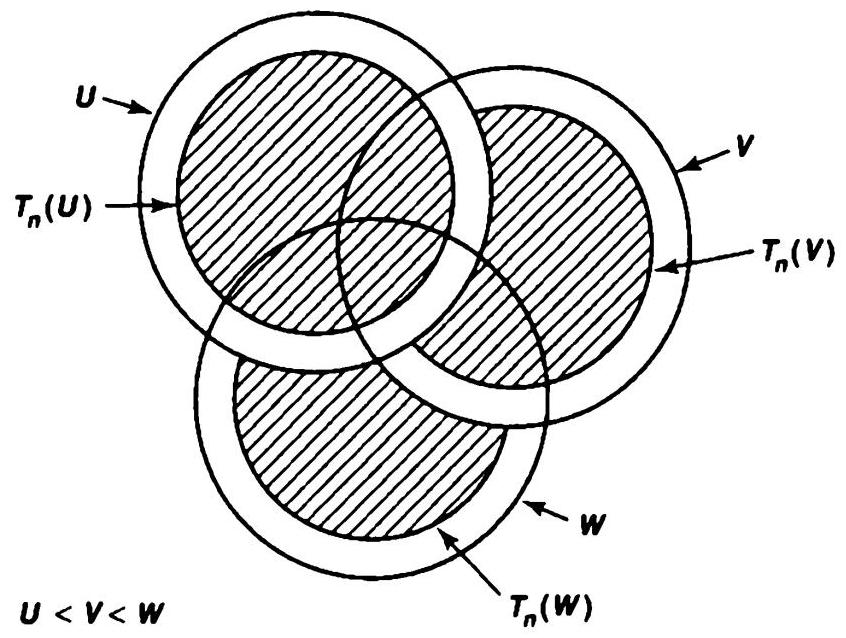
\includegraphics[width=0.7\textwidth]{images/39.1.jpg}
\end{center}
\hspace*{3em} 

Figure 39.1

In fact, they are separated by a distance of at least \(1/n\) . This means that if \(V\) and \(W\) are distinct elements of \(\mathcal{A}\) , then \(d\left( {x,y}\right)  \geq  1/n\) whenever \(x \in  {T}_{n}\left( V\right)\) and \(y \in  {T}_{n}\left( W\right)\) .

To prove this fact, assume the notation has been so chosen that \(V < W\) . Since \(x\) is in \({T}_{n}\left( V\right)\) , then \(x\) is in \({S}_{n}\left( V\right)\) , so the \(1/n\) -neighborhood of \(x\) lies in \(V\) . On the other hand, since \(V < W\) and \(y\) is in \({T}_{n}\left( W\right)\) , the definition of the latter set tells us that \(y\) is not in \(V\) . It follows that \(y\) is not in the \(1/n\) -neighborhood of \(x\) .

The sets \({T}_{n}\left( U\right)\) are not yet the ones we want, for we do not know that they are open sets. (In fact, they are closed.) So let us expand each of them slightly to obtain an open set \({E}_{n}\left( U\right)\) . Specifically, let \({E}_{n}\left( U\right)\) be the \(1/{3n}\) -neighborhood of \({T}_{n}\left( U\right)\) ; that is, let \({E}_{n}\left( U\right)\) be the union of the open balls \(B\left( {x,1/{3n}}\right)\) , for \(x \in  {T}_{n}\left( U\right)\)

In the case \(U < V < W\) , we have the situation pictured in Figure 39.2. As the figure suggests, the sets we have formed are disjoint. Indeed, if \(V\) and \(W\) are distinct elements of \(\mathcal{A}\) , we assert that \(d\left( {x,y}\right)  \geq  1/{3n}\) whenever \(x \in  {E}_{n}\left( V\right)\) and \(y \in  {E}_{n}\left( W\right)\) ; this fact follows at once from the triangle inequality. Note that for each \(V \in  \mathcal{A}\) , the set \({E}_{n}\left( V\right)\) is contained in \(V\) .

\begin{center}
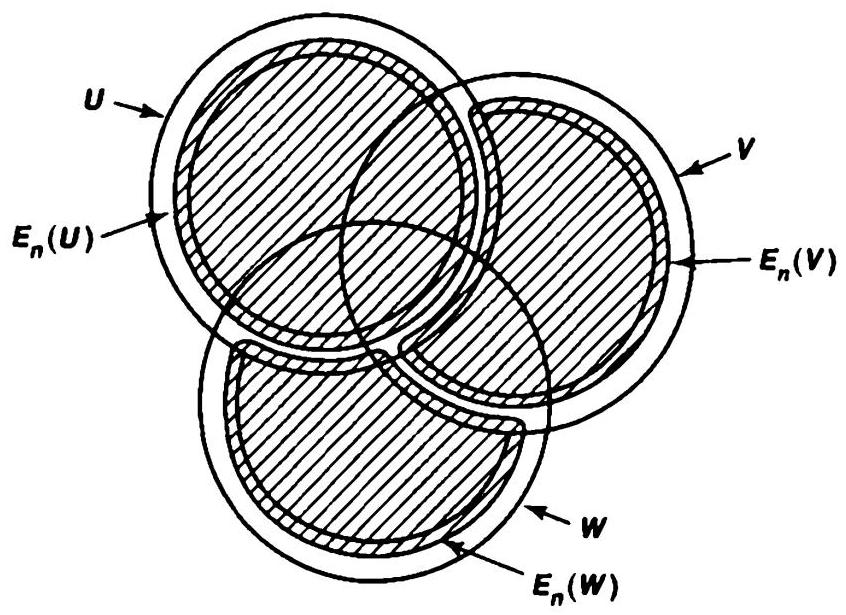
\includegraphics[width=0.7\textwidth]{images/39.2.jpg}
\end{center}
\hspace*{3em} 

Figure 39.2

Now let us define

\[
{\mathcal{E}}_{n} = \left\{  {{E}_{n}\left( U\right)  \mid  U \in  \mathcal{A}}\right\}
\]

We claim that \({\mathcal{E}}_{n}\) is a locally finite collection of open sets that refines \(\mathcal{A}\) . The fact that \({\mathcal{E}}_{n}\) refines \(\mathcal{A}\) comes from the fact that \({E}_{n}\left( V\right)  \subset  V\) for each \(V \in  \mathcal{A}\) . The fact that \({\mathcal{E}}_{n}\) is locally finite comes from the fact that for any \(x\) in \(X\) , the \(1/{6n}\) -neighborhood of \(x\) can intersect at most one element of \({\mathcal{E}}_{n}\) .

Of course, the collection \({\mathcal{E}}_{n}\) , will not cover \(X\) . (Figure 39 2 illustrates that fact.) But we assert that the collection

\[
\varepsilon  = \mathop{\bigcup }\limits_{{n \in  {\mathbb{Z}}_{ + }}}{\varepsilon }_{n}
\]

does cover \(X\) .

Let \(x\) be a point of \(X\) . The collection \(\mathcal{A}\) with which we began covers \(X\) ; let us choose \(U\) to be the first element of \(\mathcal{A}\) (in the well-ordering \(<\) ) that contains \(x\) . Since \(U\) is open, we can choose \(n\) so that \(B\left( {x,1/n}\right)  \subset  U\) Then, by definition, \(x \in  {S}_{n}\left( U\right)\) . Now because \(U\) is the first element of \(\mathcal{A}\) that contains \(x\) , the point \(x\) belongs to \({T}_{n}\left( U\right)\) . Then \(x\) also belongs to the element \({E}_{n}\left( U\right)\) of \({\mathcal{E}}_{n}\) , as desired.
\end{proof}
\section*{Exercises}
\begin{enumerate}[itemsep=0.4em, parsep=0pt, topsep=0pt, partopsep=0pt, leftmargin=*, label=\arabic*., ref=\arabic*]
\item Check the statements in Example 1.
\item Find a \idx{Point-finite collection} point-finite open covering \(\mathcal{A}\) of \(\mathbb{R}\) that is not locally finite. (The collection \(\mathcal{A}\) is point-finite if each point of \(\mathbb{R}\) lies in only finitely many elements of \(\mathcal{A}\) .)
\item Give an example of a collection of sets \(\mathcal{A}\) that is not locally finite, such that the collection \(\mathcal{B} = \{ \bar{A} \mid  A \in  \mathcal{A}\}\) is locally finite.
\item Let \(\mathcal{A}\) be the following collection of subsets of \(\mathbb{R}\) : \[ A = \{ \left( {n,n + 2}\right)  \mid  n \in  \mathbb{Z}\} \] Which of the following collections refine \(\mathcal{A}\) ? \[ \mathcal{B} = \{ \left( {x,x + 1}\right)  \mid  x \in  \mathbb{R}\} , \] \[ \mathcal{C} = \left\{  {\left( {n,n + \frac{3}{2}}\right)  \mid  n \in  \mathbb{Z}}\right\}  , \] \[ \mathcal{D} = \left\{  {\left( {x,x + \frac{3}{2}}\right)  \mid  x \in  \mathbb{R}}\right\}  . \]
\item Show that if \(X\) has a countable basis, a collection \(\mathcal{A}\) of subsets of \(X\) is countably locally finite if and only if it is countable
\item Consider \({\mathbb{R}}^{\omega }\) in the uniform topology. Given \(n\) , let \({\mathcal{B}}_{n}\) be the collection of all subsets of \({\mathbb{R}}^{\omega }\) of the form \(\prod {A}_{i}\) , where \({A}_{i} = \mathbb{R}\) for \(i \leq  n\) and \({A}_{i}\) equals either \(\{ 0\}\) or \(\{ 1\}\) otherwise. Show that the collection \(\mathcal{B} = \bigcup {\mathcal{B}}_{n}\) is countably locally finite, but neither countable nor locally finite.
\end{enumerate}
\section*{§ 40 The Nagata-Smirnov Metrization Theorem}

Now we prove that regularity of \(X\) and the existence of a countably locally finite basis for \(X\) are equivalent to metrizability of \(X\) .

The proof that these conditions imply metrizability follows very closely the second proof we gave of the Urysohn metrization theorem. In that proof we constructed a map of the space \(X\) into \({\mathbb{R}}^{\omega }\) that was an imbedding relative to the uniform metric \(\widetilde{\rho }\) on \({\mathbb{R}}^{\omega }\) . So let us review the major elements of that proof. The first step of the proof was to prove that every regular space \(X\) with a countable basis is normal. The second step was to construct a countable collection \(\left\{  {f}_{n}\right\}\) of real-valued functions on \(X\) that separated points from closed sets. The third step was to use the functions \({f}_{n}\) to define a map imbedding \(X\) in the product space \({\mathbb{R}}^{\omega }\) . And the fourth step was to show that if \({f}_{n}\left( x\right)  \leq  1/n\) for all \(x\) , then this map actually imbeds \(X\) in the metric space \(\left( {{\mathbb{R}}^{\omega },\bar{\rho }}\right)\) .

Each of these steps needs to be generalized in order to prove the general metrization theorem. First, we show that a regular space \(X\) with a basis that is countably locally finite is normal. Second, we construct a certain collection of real-valued functions \(\left\{  {f}_{\alpha }\right\}\) on \(X\) that separates points from closed sets. Third, we use these functions to imbed \(X\) in the product space \({\mathbb{R}}^{J}\) , for some \(J\) . And fourth, we show that if the functions \({f}_{\alpha }\) are sufficiently small, this map actually imbeds \(X\) in the metric space \(\left( {{\mathbb{R}}^{J},\bar{\rho }}\right)\)

Before we start, we need to recall a notion we have already introduced in the exercises, that of a \({G}_{\delta }\) set.

\begin{definition}
	A subset \(A\) of a space \(X\) is called a \({G}_{\delta }\) set in \(X\) if it equals the intersection of a countable collection of open subsets of \(X\) .
\end{definition}

\begin{centeredblock}
\begin{example}
	Each open subset of \(X\) is a \({G}_{\delta }\) set, invially In a first-countable Hausdorff space, each one-point set is a \({G}_{\delta }\) set The one-point subset \(\{ \Omega \}\) of \({\bar{S}}_{\Omega }\) is not a \({G}_{\delta }\) set, as you can check
\end{example}
\end{centeredblock}

\begin{centeredblock}
\begin{example}
	In a metric space \(X\) , each closed set is a \({G}_{\delta }\) set. Given \(A \subset  X\) , let \(U\left( {A,\epsilon }\right)\) denote the \(\epsilon\) -neighborhood of \(A\) If \(A\) is closed, you can check that

\[
A = \mathop{\bigcap }\limits_{{n \in  {\mathbb{Z}}_{ + }}}U\left( {A,1/n}\right)
\]
\end{example}
\end{centeredblock}

\begin{lemma}
	Let \(X\) be a regular space with a basis \(\mathcal{B}\) that is countably locally finite. Then \(X\) is normal, and every closed set in \(X\) is a \({G}_{\delta }\) set in \(X\) .
\end{lemma}

\begin{proof}
	Step 1. Let \(W\) be open in \(X\) . We show there is a countable collection \(\left\{  {U}_{n}\right\}\) of open sets of \(X\) such that
\[
W = \bigcup {U}_{n} = \bigcup {\bar{U}}_{n}
\]

Since the basis \(\mathcal{B}\) for \(X\) is countably locally finite, we can write \(\mathcal{B} = \bigcup {\mathcal{B}}_{n}\) , where each collection \({\mathcal{B}}_{n}\) is locally finite. Let \({\mathcal{C}}_{n}\) be the collection of those basis elements \(B\) such that \(B \in  {\mathcal{B}}_{n}\) and \(\bar{B} \subset  W\) . Then \({\mathcal{C}}_{n}\) is locally finite, being a subcollection of \({\mathcal{B}}_{n}\) Define

\[
{U}_{n} = \mathop{\bigcup }\limits_{{B \in  {\mathcal{C}}_{n}}}B
\]

Then \({U}_{n}\) is an open set, and by Lemma 39 1,

\[
{\bar{U}}_{n} = \mathop{\bigcup }\limits_{{B \in  {\mathcal{C}}_{n}}}\bar{B}.
\]

Therefore, \({\bar{U}}_{n} \subset  W\) , so that

\[
\bigcup {U}_{n} \subset  \bigcup {\bar{U}}_{n} \subset  W
\]

We assert that equality holds. Given \(x \in  W\) , there is by regularity a basis element \(B \in  \mathcal{B}\) such that \(x \in  B\) and \(\bar{B} \subset  W\) . Now \(B \in  {\mathcal{B}}_{n}\) for some \(n\) . Then \(B \in  {\mathcal{C}}_{n}\) by definition, so that \(x \in  {U}_{n}\) . Thus \(W \subset  \bigcup {U}_{n}\) , as desired.

Step 2. We show that every closed set \(C\) in \(X\) is a \({G}_{\delta }\) set in \(X\) Given \(C\) , let \(W = X - C\) . By Step 1, there are sets \({U}_{n}\) in \(X\) such that \(W = \bigcup {U}_{n}\) Then

\[
C = \bigcap \left( {X - {\bar{U}}_{n}}\right)
\]

so that \(C\) equals a countable intersection of open sets of \(X\) .

Step 3. We show \(X\) is normal Let \(C\) and \(D\) be disjoint closed sets in \(X\) . Applying Step 1 to the open set \(X - D\) , we construct a countable collection \(\left\{  {U}_{n}\right\}\) of open sets such that \(\mathop{\bigcup }\limits_{n}{U}_{n} = \mathop{\bigcup }\limits_{n}{\bar{U}}_{n} = X - D\) . Then \(\left\{  {U}_{n}\right\}\) covers \(C\) and each set \({\bar{U}}_{n}\) is disjoint from \(D\) . Similarly, there is a countable covering \(\left\{  {V}_{n}\right\}\) of \(D\) by open sets whose closures are disjoint from \(C\) .

Now we are back in the situation that arose in the proof that a regular space with a countable basis is normal (Theorem 32.1). We can repeat that proof verbatim. Define

\[
{U}_{n}^{\prime } = {U}_{n} - \mathop{\bigcup }\limits_{{i = 1}}^{n}{\bar{V}}_{i}\;\text{ and }\;{V}_{n}^{\prime } = {V}_{n} - \mathop{\bigcup }\limits_{{i = 1}}^{n}{\bar{U}}_{i}
\]

Then the sets

\[
{U}^{\prime } = \mathop{\bigcup }\limits_{{n \in  {\mathbb{Z}}_{ + }}}{U}_{n}^{\prime }\;\text{ and }\;{V}^{\prime } = \mathop{\bigcup }\limits_{{n \in  {\mathbb{Z}}_{ + }}}{V}_{n}^{\prime }
\]

are disjoint open sets about \(C\) and \(D\) , respectively.
\end{proof}
\begin{lemma}
	Let \(X\) be normal; let \(A\) be a closed \({G}_{\delta }\) set in \(X\) . Then there is a continuous function \(f : X \rightarrow  \left\lbrack  {0,1}\right\rbrack\) such that \(f\left( x\right)  = 0\) for \(x \in  A\) and \(f\left( x\right)  > 0\) for \(x \notin  A\) .
\end{lemma}

\begin{proof}
	We gave this as an exercise in \(\$ {33}\) , we provide a proof here. Write \(A\) as the intersection of the open sets \({U}_{n}\) , for \(n \in  {\mathbb{Z}}_{ + }\) For each \(n\) , choose a continuous function \({f}_{n} : X \rightarrow  \left\lbrack  {0,1}\right\rbrack\) such that \(f\left( x\right)  = 0\) for \(x \in  A\) and \(f\left( x\right)  = 1\) for \(x \in  X - {U}_{n}\) Define \(f\left( x\right)  = \sum {f}_{n}\left( x\right) /{2}^{n}\) The series converges uniformly, by comparison with \(\sum 1/{2}^{n}\) , so that \(f\) is continuous. Also, \(f\) vanishes on \(A\) and is positive on \(X - A\)
\end{proof}
\begin{theorem}[\idx{Nagata-Smirnov metrization theorem}]
	A space \(X\) is metrizable if and only if \(X\) is regular and has a basis that is countably locally finite.
\end{theorem}

\begin{proof}
	Step 1. Assume \(X\) is regular with a countably locally finite basis \(\mathcal{B}\) Then \(X\) is normal, and every closed set in \(X\) is a \({G}_{\delta }\) set in \(X\) . We shall show that \(X\) is metrizable by imbedding \(X\) in the metric space \(\left( {{\mathbb{R}}^{J},\bar{\rho }}\right)\) for some \(J\)
Let \(\mathcal{B} = \bigcup {\mathcal{B}}_{n}\) , where each collection \({\mathcal{B}}_{n}\) is locally finite. For each positive integer \(n\) , and each basis element \(B \in  {\mathcal{B}}_{n}\) , choose a continuous function

\[
{f}_{n,B} : X \rightarrow  \left\lbrack  {0,1/n}\right\rbrack
\]

such that \({f}_{n,B}\left( x\right)  > 0\) for \(x \in  B\) and \({f}_{n,B}\left( x\right)  = 0\) for \(x \notin  B\) . The collection \(\left\{  {f}_{n,B}\right\}\) separates points from closed sets in \(X\) . Given a point \({x}_{0}\) and a neighborhood \(U\) of \({x}_{0}\) , there is a basis element \(B\) such that \({x}_{0} \in  B \subset  U\) . Then \(B \in  {\mathcal{B}}_{n}\) for some \(n\) , so that \({f}_{n,B}\left( {x}_{0}\right)  > 0\) and \({f}_{n,B}\) vanishes outside \(U\) .

Let \(J\) be the subset of \({\mathbb{Z}}_{ + } \times  \mathcal{B}\) consisting of all pairs(n, B)such that \(B\) is an element of \({\mathcal{B}}_{n}\) . Define

\[
F : X \rightarrow  {\left\lbrack  0,1\right\rbrack  }^{J}
\]

by the equation

\[
F\left( x\right)  = \left( {{f}_{n,B}\left( x\right) }\right) \left( {n,b}\right)  \in  J.
\]

Relative to the product topology on \({\left\lbrack  0,1\right\rbrack  }^{J}\) , the map \(F\) is an imbedding, by Theorem 34.2.

Now we give \({\left\lbrack  0,1\right\rbrack  }^{J}\) the topology induced by the uniform metric and show that \(F\) is an imbedding relative to this topology as well. Here is where the condition \({f}_{n,B}\left( x\right)  < 1/n\) comes in. The uniform topology is finer (larger) than the product topology. Therefore, relative to the uniform metric, the map \(F\) is injective and carries open sets of \(X\) onto open sets of the image space \(Z = F\left( X\right)\) We must give a separate proof that \(F\) is continuous.

Note that on the subspace \({\left\lbrack  0,1\right\rbrack  }^{J}\) of \({\mathbb{R}}^{J}\) , the uniform metric equals the metric

\[
\rho \left( {\left( {x}_{\alpha }\right) ,\left( {y}_{\alpha }\right) }\right)  = \sup \left\{  \left| {{x}_{\alpha } - {y}_{\alpha }}\right| \right\}  .
\]

To prove continuity, we take a point \({x}_{0}\) of \(X\) and a number \(\epsilon  > 0\) , and find a neighborhood \(W\) of \({x}_{0}\) such that

\[
x \in  W \Rightarrow  \rho \left( {F\left( x\right) ,F\left( {x}_{0}\right) }\right)  < \epsilon
\]

Let \(n\) be fixed for the moment. Choose a neighborhood \({U}_{n}\) of \({x}_{0}\) that intersects only finitely many elements of the collection \({\mathcal{B}}_{n}\) . This means that as \(B\) ranges over \({\mathcal{B}}_{n}\) , all but finitely many of the functions \({f}_{n,B}\) are identically equal to zero on \({U}_{n}\) . Because each function \({f}_{n,B}\) is continuous, we can now choose a neighborhood \({V}_{n}\) of \({x}_{0}\) contained in \({U}_{n}\) on which each of the remaining functions \({f}_{n,B}\) , for \(B \in  {\mathcal{B}}_{n}\) , varies by at most \(\epsilon /2\) .

Choose such a neighborhood \({V}_{n}\) of \({x}_{0}\) for each \(n \in  {\mathbb{Z}}_{ + }\) . Then choose \(N\) so that \(1/N \leq  \epsilon /2\) , and define \(W = {V}_{1} \cap  \cdots  \cap  {V}_{N}\) We assert that \(W\) is the desired neighborhood of \({x}_{0}\) . Let \(x \in  W\) . If \(n \leq  N\) , then

\[
\left| {{f}_{n,B}\left( x\right)  - {f}_{n,B}\left( {x}_{0}\right) }\right|  \leq  \epsilon /2
\]

because the function \({f}_{n,B}\) either vanishes identically or varies by at most \(\epsilon /2\) on \(W\) . If \(n > N\) , then

\[
\left| {{f}_{n,B}\left( x\right)  - {f}_{n,B}\left( {x}_{0}\right) }\right|  \leq  1/n < \epsilon /2
\]

because \({f}_{n,B}\) maps \(X\) into \(\left\lbrack  {0,1/n}\right\rbrack\) . Therefore,

\[
\rho \left( {F\left( x\right) ,F\left( {x}_{0}\right) }\right)  \leq  \epsilon /2 < \epsilon ,
\]

as desired.

Step 2. Now we prove the converse. Assume \(X\) is metrizable. We know \(X\) is regular; let us show that \(X\) has a basis that is countably locally finite.

Choose a metric for \(X\) . Given \(m\) , let \({A}_{m}\) be the covering of \(X\) by all open balls of radius \(1/m\) . By Lemma 39.2, there is an open covering \({\mathcal{B}}_{m}\) of \(X\) refining \({\mathcal{A}}_{m}\) such that \({\mathcal{B}}_{m}\) is countably locally finite. Note that each element of \({\mathcal{B}}_{m}\) has diameter at most \(2/m\) Let \(\mathcal{B}\) be the union of the collections \({\mathcal{B}}_{m}\) , for \(m \in  {\mathbb{Z}}_{ + }\) . Because each collection \({\mathcal{B}}_{m}\) is countably locally finite, so is \(\mathcal{B}\) . We show that \(\mathcal{B}\) is a basis for \(X\) .

Given \(x \in  X\) and given \(\epsilon  > 0\) , we show that there is an element \(B\) of \(\mathcal{B}\) containing \(x\) that is contained in \(B\left( {x,\epsilon }\right)\) . First choose \(m\) so that \(1/m < \epsilon /2\) . Then, because \({\mathcal{B}}_{m}\) covers \(X\) , we can choose an element \(B\) of \({\mathcal{B}}_{m}\) that contains \(x\) . Since \(B\) contains \(x\) and has diameter at most \(2/m < \epsilon\) , it is contained in \(B\left( {x,\epsilon }\right)\) , as desired.
\end{proof}
\section*{Exercises}
\begin{enumerate}[itemsep=0.4em, parsep=0pt, topsep=0pt, partopsep=0pt, leftmargin=*, label=\arabic*., ref=\arabic*]
\item Check the details of Examples 1 and 2.
\item A subset \(W\) of \(X\) is said to be an `` \({F}_{\sigma }\) set'' in \(X\) if \(W\) equals a countable union of closed sets of \(X\) . Show that \(W\) is an \({F}_{\sigma }\) set in \(X\) if and only if \(X - W\) is a \({G}_{\delta }\) set in \(X\) . [The termunology comes from the French. The ``F'' stands for ``fermé,'' which means ``closed,'' and the `` \(\sigma\) `` for ``somme,'' which means ``union.'']
\item Many spaces have countable bases; but no \({T}_{1}\) space has a locally finite basis unless it is discrete. Prove this fact.
\item Find a nondiscrete space that has a countably locally finite basis but does not have a countable basis.
\item A collection \(\mathcal{A}\) of subsets of \(X\) is said to be \idx{locally discrete} if each point of \(X\) has a neighborhood that intersects at most one element of \(\mathcal{A}\) . A collection \(\mathcal{B}\) is \idx{countably locally discrete} (or `` \(\sigma\) -locally discrete'') if it equals a countable union of locally discrete collections. Prove the following: \textsl{Theorem. (\idx{Bing metrization theorem}).} A space \(X\) is metrizable if and only if it is regular and has a basis that is countably locally discrete. 
\end{enumerate}
\section*{§ 41 Paracompactness}

The concept of paracompactness is one of the most useful generalizations of compactness that has been discovered in recent years. It is particularly useful for applications in topology and differential geometry We shall give just one application, a metrization theorem that we prove in the next section.

Many of the spaces that are familiar to us already are paracompact. For instance, every compact space is paracompact, this will be an immediate consequence of the definition. It is also true that every metrizable space is paracompact, this is a theorem due to A. H. Stone, which we shall prove. Thus the class of \idx{paracompact space}s includes the two most important classes of spaces we have studied. It includes many other spaces as well.

To see how paracompactness generalizes compactness, we recall the definition of compactness: A space \(X\) is said to be compact if every open covering \(\mathcal{A}\) of \(X\) contains a finite subcollection that covers \(X\) . An equivalent way of saying this is the following:

A space \(X\) is compact if every open covering \(\mathcal{A}\) of \(X\) has a finite open refinement \(\mathcal{B}\) that covers \(X\)

This definition is equivalent to the usual one, given such a refinement \(\mathcal{B}\) , one can choose for each element of \(\mathcal{B}\) an element of \(\mathcal{A}\) containing it; in this way one obtains a finite subcollection of \(\mathcal{A}\) that covers \(X\) .

This new formulation of compactness is an awkward one, but it suggests a way to generalize.

\begin{definition}
	A space \(X\) is paracompact if every open covering \(\mathcal{A}\) of \(X\) has a locally finite open refinement \(\mathcal{B}\) that covers \(X\) .
\end{definition}

Many authors, following the lead of Bourbaki, include as part of the definition of the term paracompact the requirement that the space be Hausdorff. (Bourbaki also includes the Hausdorff condition as part of the definition of the term compact.) We shall not follow this convention.

\begin{centeredblock}
\begin{example}
	The space \({\mathbb{R}}^{n}\) is paracompact Let \(X = {\mathbb{R}}^{n}\) Let \(\mathcal{A}\) be an open covering of \(X\) . Let \({B}_{0} = \varnothing\) , and for each positive integer \(m\) , let \({B}_{m}\) denote the open ball of radius \(m\) centered at the origin. Given \(m\) , choose finitely many elements of \(\mathcal{A}\) that cover \({\widetilde{B}}_{m}\) and intersect each one with the open set \(X - {\bar{B}}_{m - 1}\) , let this finite collection of open sets be denoted \({\mathcal{C}}_{m}\) Then the collection \(\mathcal{C} = \bigcup {\mathcal{C}}_{m}\) is a refinement of \(\mathcal{A}\) It is clearly locally finite, for the open set \({B}_{m}\) intersects only finitely many elements of \(\mathcal{C}\) , namely those elements beloriging to the collection \({\mathcal{C}}_{1} \cup  \; \cup  {\mathcal{C}}_{m}\) . Finally, \(\mathcal{C}\) covers \(X\) For, given \(x\) , let \(m\) be the smallest integer such that \(x \in  {\bar{B}}_{m}\) . Then \(x\) belongs to an element of \({\mathcal{C}}_{m}\) , by definition.
\end{example}
\end{centeredblock}

Some of the properties of a paracompact space are similar to those of a compact space. For instance, a subspace of a paracompact space is not necessarily paracompact; but a closed subspace is paracompact. Also, a paracompact Hausdorff space is normal. In other ways, a paracompact space is not similar to a compact space; in particular, the product of two paracompact spaces need not be paracompact. We shall verify these facts shortly.

\section*{Theorem 41.1. Every paracompact Hausdorff space \(X\) is normal}

Proof The proof is somewhat similar to the proof that a compact Hausdorff space is normal.

First one proves regularity Let \(a\) be a point of \(X\) and let \(B\) be a closed set of \(X\) disjoint from \(a\) . The Hausdorff condition enables us to choose, for each \(b\) in \(B\) , an open set \({U}_{b}\) about \(b\) whose closure is disjoint from \(a\) . Cover \(X\) by the open sets \({U}_{b}\) , along with the open set \(X - B\) ; take a locally finite open refinement \(\mathcal{C}\) that covers \(X\) . Form the subcollection \(\mathcal{D}\) of \(\mathcal{C}\) consisting of every element of \(\mathcal{C}\) that intersects \(B\) . Then \(\mathcal{D}\) covers \(B\) . Furthermore, if \(D \in  \mathcal{D}\) , then \(\bar{D}\) is disjoint from \(a\) . For \(D\) intersects \(B\) , so it lies in some set \({U}_{b}\) , whose closure is disjoint from \(a\) . Let

\[
V = \mathop{\bigcup }\limits_{{D \in  \mathcal{D}}}D
\]

then \(V\) is an open set in \(X\) containing \(B\) . Because \(\mathcal{D}\) is locally finite,

\[
\bar{V} = \mathop{\bigcup }\limits_{{D \in  \mathcal{D}}}\bar{D}
\]

so that \(\bar{V}\) is disjoint from \(a\) . Thus regularity is proved.

To prove normality, one merely repeats the same argument, replacing \(a\) by the closed set \(A\) throughout and replacing the Hausdorff condition by regularity.

\section*{Theorem 41.2. Every closed subspace of a paracompact space is paracompact.}

\begin{proof}
	Let \(Y\) be a closed subspace of the paracompact space \(X\) ; let \(\mathcal{A}\) be a covering of \(Y\) by sets open in \(Y\) . For each \(A \in  \mathcal{A}\) , choose an open set \({A}^{\prime }\) of \(X\) such that \({A}^{\prime } \cap  Y = A\) . Cover \(X\) by the open sets \({A}^{\prime }\) , along with the open set \(X - Y\) . Let \(\mathcal{B}\) be a locally finite open refinement of this covering that covers \(X\) . The collection
\[
\mathcal{C} = \{ B \cap  Y \mid  B \in  \mathcal{B}\}
\]

is the required locally finite open refinement of \(\mathcal{A}\)

\begin{centeredblock}
\begin{example}
	A paracompact subspace of a Hausdorff space X need not be closed in X. Indeed, the open interval(0,1)is paracompact, being homeomorphic to \(\mathbb{R}\) , but it is not closed in \(\mathbb{R}\)
\end{example}
\end{centeredblock}

\begin{centeredblock}
\begin{example}
	A subspace of a paracompact space need not be paracompact The space \({\bar{S}}_{\Omega } \times  {\bar{S}}_{\Omega }\) is compact and, therefore, paracompact. But the subspace \({S}_{\Omega } \times  {\bar{S}}_{\Omega }\) is not para-compact, for it is Hausdorff but not normal.
\end{example}
\end{centeredblock}

To prove the important theorem that every metrizable space is paracompact, we need the following lemma, due to E. Michael, which is also useful for other purposes:
\end{proof}
\begin{lemma}
	Let \(X\) be regular. Then the following conditions on \(X\) are equivalent: Every open covering of \(X\) has a refinement that is:

(1) An open covering of \(X\) and countably locally finite.

(2) A covering of \(X\) and locally finite.

(3) A closed covering of \(X\) and locally finite.

(4) An open covering of \(X\) and locally finite.
\end{lemma}

\begin{proof}
	It is trivial that \(\left( 4\right)  \Rightarrow  \left( 1\right)\) . What we need to prove our theorem is the converse In order to prove the converse, we must go through the steps \(\left( 1\right)  \Rightarrow  \left( 2\right)  \Rightarrow  \left( 3\right)  \Rightarrow  \left( 4\right)\) anyway, so we have for convenience listed these conditions in the statement of the lemma.
(1) \(\Rightarrow\) (2). Let \(\mathcal{A}\) be an open covering of \(X\) . Let \(\mathcal{B}\) be an open refinement of \(\mathcal{A}\) that covers \(X\) and is countably locally finite; let

\[
\mathcal{B} = \bigcup {\mathcal{B}}_{n}
\]

where each \({\mathcal{B}}_{n}\) is locally finite.

Now we apply essentially the same sort of shrinking trick we have used before to make sets from different \({\mathcal{B}}_{n}\) 's disjoint. Given \(i\) , let

\[
{V}_{i} = \mathop{\bigcup }\limits_{{U \in  {\mathcal{B}}_{i}}}U
\]

Then for each \(n \in  {\mathbb{Z}}_{ + }\) and each element \(U\) of \({\mathcal{B}}_{n}\) , define

\[
{S}_{n}\left( U\right)  = U - \mathop{\bigcup }\limits_{{i < n}}{V}_{i}
\]

[Note that \({S}_{n}\left( U\right)\) is not necessarily open, nor closed.] Let

\[
{\mathcal{C}}_{n} = \left\{  {{S}_{n}\left( U\right)  \mid  U \in  {\mathcal{B}}_{n}}\right\}
\]

Then \({\mathcal{C}}_{n}\) is a refinement of \({\mathcal{B}}_{n}\) , because \({S}_{n}\left( U\right)  \subset  U\) for each \(U \in  {\mathcal{B}}_{n}\) .

Let \(\mathcal{C} = \bigcup {\mathcal{C}}_{n}\) . We assert that \(\mathcal{C}\) is the required locally finite refinement of \(\mathcal{A}\) , covering \(X\)

Let \(x\) be a point of \(X\) . We wish to prove that \(x\) lies in an element of \(\mathcal{C}\) , and that \(x\) has a neighborhood intersecting only finitely many elements of \(\mathcal{C}\) . Consider the covering \(\mathcal{B} = \bigcup {\mathcal{B}}_{n}\) ; let \(N\) be the smallest integer such that \(x\) lies in an element of \({\mathcal{B}}_{N}\) . Let \(U\) be an element of \({\mathcal{B}}_{N}\) containing \(x\) . First, note that since \(x\) lies in no element of \({\mathcal{B}}_{i}\) for \(i < N\) , the point \(x\) lies in the element \({S}_{N}\left( U\right)\) of \(\mathcal{C}\) . Second, note that since each collection \({\mathcal{B}}_{n}\) is locally finite, we can choose for each \(n = 1,\ldots ,N\) a neighborhood \({W}_{n}\) of \(x\) that intersects only finitely many elements of \({\mathcal{B}}_{n}\) . Now if \({W}_{n}\) intersects the element \({S}_{n}\left( V\right)\) of \({\mathcal{C}}_{n}\) , it must intersect the element \(V\) of \({\mathcal{B}}_{n}\) , since \({S}_{n}\left( V\right)  \subset  V\) . Therefore, \({W}_{n}\) intersects only finitely many elements of \({\mathcal{C}}_{n}\) . Furthermore, because \(U\) is in \({\mathcal{B}}_{N},U\) intersects no element of \({\mathcal{C}}_{n}\) for \(n > N\) As a result, the neighborhood

\[
{W}_{1} \cap  {W}_{2} \cap  \cdots  \cap  {W}_{N} \cap  U
\]

of \(x\) intersects only finitely many elements of \(\mathcal{C}\) .

\(\left( 2\right)  \Rightarrow  \left( 3\right)\) Let \(\mathcal{A}\) be an open covering of \(X\) . Let \(\mathcal{B}\) be the collection of all open sets \(U\) of \(X\) such that \(\bar{U}\) is contained in an element of \(\mathcal{A}\) . By regularity, \(\mathcal{B}\) covers \(X\) . Using (2), we can find a refinement \(\mathcal{C}\) of \(\mathcal{B}\) that covers \(X\) and is locally finite. Let

\[
\mathcal{D} = \{ \bar{C} \mid  C \in  \mathcal{C}\} .
\]

Then \(\mathcal{D}\) also covers \(X\) ; it is locally finite by Lemma 39.1; and it refines \(\mathcal{A}\) .

\(\left( 3\right)  \Rightarrow  \left( 4\right)\) . Let \(\mathcal{A}\) be an open covering of \(X\) . Using(3), choose \(\mathcal{B}\) to be a refinement of \(\mathcal{A}\) that covers \(X\) and is locally finite (We can take \(\mathcal{B}\) to be a closed refinement if we like, but that is irrelevant.) We seek to expand each element \(B\) of \(\mathcal{B}\) slightly to an open set, making the expansion slight enough that the resulting collection of open sets will still be locally finite and will still refine \(\mathcal{A}\) .

This step involves a new trick. The previous trick, used several times, consisted of ordering the sets in some way and forming a new set by subtracting off all the previous ones. That trick shrinks the sets; to expand them we need something different. We shall introduce an auxiliary locally finite closed covering \(\mathcal{C}\) of \(X\) and use it to expand the elements of \(\mathcal{B}\) .

For each point \(x\) of \(X\) , there is a neighborhood of \(x\) that intersects only finitely many elements of \(\mathcal{B}\) . The collection of all open sets that intersect only finitely many elements of \(\mathcal{B}\) is thus an open covering of \(X\) . Using (3) again, let \(\mathcal{C}\) be a closed refinement of this covering that covers \(X\) and is locally finite. Each element of \(\mathcal{C}\) intersects only finitely many elements of \(\mathcal{B}\) .

For each element \(B\) of \(B\) , let

\[
\mathcal{C}\left( B\right)  = \{ C \mid  C \in  \mathcal{C}\text{ and }C \subset  X - B\}
\]

Then define

\[
E\left( B\right)  = X - \mathop{\bigcup }\limits_{{C \in  C\left( B\right) }}C.
\]

Because \(\mathcal{C}\) is a locally finite collection of closed sets, the union of the elements of any subcollection of \(\mathcal{C}\) is closed, by Lemma 39.1. Therefore, the set \(E\left( B\right)\) is an open set. Furthermore, \(E\left( B\right)  \supset  B\) by definition. (See Figure 41 1, in which the elements of \(\mathcal{B}\) are represented as closed circular regions and line segments, and the elements of \(\mathcal{C}\) are represented as closed square regions.)

\begin{center}
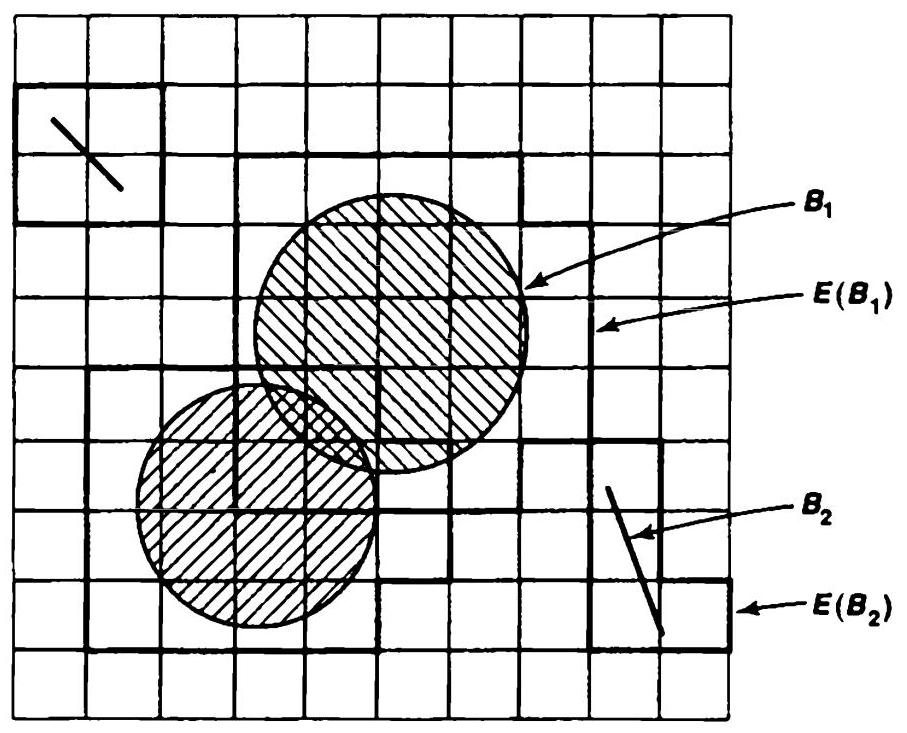
\includegraphics[width=0.8\textwidth]{images/41.1.jpg}
\end{center}
\hspace*{3em} 

Figure 41.1

Now we may have expanded each \(B\) too much; the collection \(\{ E\left( B\right) \}\) may not be a refinement of \(\mathcal{A}\) . This is easily remedied. For each \(B \in  \mathcal{B}\) , choose an element \(F\left( B\right)\) of \(\mathcal{A}\) containing \(B\) . Then define

\[
\mathcal{D} = \{ E\left( B\right)  \cap  F\left( B\right)  \mid  B \in  \mathcal{B}\} .
\]

The collection \(\mathcal{D}\) is a refinement of \(\mathcal{A}\) . Because \(B \subset  \left( {E\left( B\right)  \cap  F\left( B\right) }\right)\) and \(\mathcal{B}\) covers \(X\) , the collection \(\mathcal{D}\) also covers \(X\)

We have finally to prove that \(\mathcal{D}\) is locally finite. Given a point \(x\) of \(X\) , choose a neighborhood \(W\) of \(x\) that intersects only finitely many elements of \(\mathcal{C}\) , say \({C}_{1},\ldots ,{C}_{k}\) We show that \(W\) intersects only finitely many elements of \(\mathcal{D}\) . Because \(\mathcal{C}\) covers \(X\) , the set \(W\) is covered by \({C}_{1},\ldots ,{C}_{k}\) . Thus, it suffices to show that each element \(C\) of \(\mathcal{C}\) intersects only finitely many elements of \(\mathcal{D}\) . Now if \(C\) intersects the set \(E\left( B\right)  \cap  F\left( B\right)\) , then it intersects \(E\left( B\right)\) , so by definition of \(E\left( B\right)\) it is not contained in \(X - B\) , hence \(C\) must intersect \(B\) . Since \(C\) intersects only finitely many elements of \(\mathcal{B}\) , it can intersect at most the same number of elements of the collection \(\mathcal{D}\)
\end{proof}
\section*{Theorem 41.4. Every metrizable space is paracompact}

\begin{proof}
	Let \(X\) be a metrizable space. We already know from Lemma 39.2 that, given an open covering \(\mathcal{A}\) of \(X\) , it has an open refinement that covers \(X\) and is countably locally finite. The preceding lemma then implies that \(\mathcal{A}\) has an open refinement that covers \(X\) and is locally finite
\end{proof}
\begin{theorem}
	Every regular Lindelöf space is paracompact
\end{theorem}

\begin{proof}
	Let \(X\) be regular and Lindelof. Given an open covering \(\mathcal{A}\) of \(X\) , it has a countable subcollection that covers \(X\) , this subcollection is automatically countably locally finite The preceding lemma applies to show \(\mathcal{A}\) has an open refinement that covers \(X\) and is locally finite.
\end{proof}

\begin{centeredblock}
\begin{example}
	The product of two paracompact spaces need not be paracompact The space \({\mathbb{R}}_{\ell }\) is paracompact, for it is regular and Lindelof However, \({\mathbb{R}}_{\ell } \times  {\mathbb{R}}_{\ell }\) is not paracom-pact, for it is Hausdorff but not normal
\end{example}
\end{centeredblock}

\begin{centeredblock}
\begin{example}
	The space \({\mathbb{R}}^{\omega }\) is paracompact in both the product and uniform topologies. This result follows from the fact that \({\mathbb{R}}^{\omega }\) is metrizable in these topologies. It is not known whether \({\mathbf{R}}^{\omega }\) is paracompact in the box topology (See the comment in Exercise 5 of §32 )
\end{example}
\end{centeredblock}

\begin{centeredblock}
\begin{example}
	The product space \({\mathbb{R}}^{J}\) is not paracompact if \(J\) is uncountable For \({\mathbb{R}}^{J}\) is Hausdorff but not normal
\end{example}
\end{centeredblock}

One of the most useful properties that a paracompact space \(X\) possesses has to do with the existence of partitions of unity on \(X\) . We have already seen the finite version of this notion in \(§{36}\) , we discuss the general case now. Recall that if \(\phi : X \rightarrow  \mathbb{R}\) , the support of \(\phi\) is the closure of the set of those \(x\) for which \(\phi \left( x\right)  \neq  0\) .

\begin{definition}
	Let \({\left\{  {U}_{\alpha }\right\}  }_{\alpha  \in  J}\) be an indexed open covering of \(X\) . An indexed family of continuous functions

\[
{\phi }_{\alpha } : X \rightarrow  \left\lbrack  {0,1}\right\rbrack
\]

is said to be a partition of unity on \(X\) , dominated by \(\left\{  {U}_{\alpha }\right\}\) , if:

(1) (Support \({\phi }_{\alpha }\) ) \(\subset  {U}_{\alpha }\) for each \(\alpha\) .

(2) The indexed family \(\left\{  {\text{ Support }{\phi }_{\alpha }}\right\}\) is locally finite

(3) \(\sum {\phi }_{\alpha }\left( x\right)  = 1\) for each \(x\) .
\end{definition}

Condition (2) implies that each \(x \in  X\) has a neighborhood on which the function \({\phi }_{\alpha }\) vanishes identically for all but finitely many values of \(\alpha\) . Thus we can make sense of the ``sum'' indicated in (3); we interpret it to mean the sum of the terms \({\phi }_{\alpha }\left( x\right)\) that do not equal zero.

We now construct a partition of unity on an arbitrary paracompact Hausdorff space. We begin by proving a ``shrinking lemma,'' just as we did for the finite case in §36.

-Lemma 41.6. Let \(X\) be a paracompact Hausdorff space; let \({\left\{  {U}_{\alpha }\right\}  }_{\alpha  \in  J}\) be an indexed family of open sets covering \(X\) . Then there exists a locally finite indexed family \({\left\{  {V}_{\alpha }\right\}  }_{\alpha  \in  J}\) of open sets covering \(X\) such that \({\widetilde{V}}_{\alpha } \subset  {U}_{\alpha }\) for each \(\alpha\) .

The condition that \({\widetilde{V}}_{\alpha } \subset  {U}_{\alpha }\) for each \(\alpha\) is sometimes expressed by saying that the family \(\left\{  {\widetilde{V}}_{\alpha }\right\}\) is a \idx{precise refinement} of the family \(\left\{  {U}_{\alpha }\right\}\) .

\begin{proof}
	Let \(\mathcal{A}\) be the collection of all open sets \(A\) such that \(\bar{A}\) is contained in some element of the collection \(\left\{  {U}_{\alpha }\right\}\) . Regularity of \(X\) implies that \(\mathcal{A}\) covers \(X\) . Since \(X\) is paracompact, we can find a locally finite collection \(\mathcal{B}\) of open sets covering \(X\) that refines \(\mathcal{A}\) Let us index \(\mathcal{B}\) bijectively with some index set \(K\) , then the general element of \(\mathcal{B}\) can be denoted \({B}_{\beta }\) , for \(\beta  \in  K\) , and \({\left\{  {B}_{\beta }\right\}  }_{\beta  \in  K}\) is a locally finite indexed family. Since \(\mathcal{B}\) refines \(\mathcal{A}\) , we can define a function \(f : K \rightarrow  J\) by choosing, for each \(\beta\) in \(K\) , an element \(f\left( \beta \right)  \in  J\) such that
\[
{\bar{B}}_{\beta } \subset  {U}_{f\left( \beta \right) }.
\]

Then for each \(\alpha  \in  J\) , we define \({V}_{\alpha }\) to be the union of the elements of the collection

\[
{\mathcal{B}}_{\alpha } = \left\{  {{B}_{\beta } \mid  f\left( \beta \right)  = \alpha }\right\}  .
\]

(Note that \({V}_{\alpha }\) is empty if there exists no index \(\beta\) such that \(f\left( \beta \right)  = \alpha\) .) For each element \({B}_{\beta }\) of the collection \({\mathcal{B}}_{\alpha }\) we have \({\bar{B}}_{\beta } \subset  {U}_{\alpha }\) by definition. Because the collection \({\mathcal{B}}_{\alpha }\) is locally finite, \({\bar{V}}_{\alpha }\) equals the union of the closures of the elements of \({\mathcal{B}}_{\alpha }\) , so that \({\bar{V}}_{\alpha } \subset  {U}_{\alpha }\) .

Finally, we check local finiteness Given \(x \in  X\) , choose a neighborhood \(W\) of \(x\) such that \(W\) intersects \({B}_{\beta }\) for only finitely many values of \(\beta\) , say \(\beta  = {\beta }_{1},\ldots ,{\beta }_{K}\) . Then \(W\) can intersect \({V}_{\alpha }\) only if \(\alpha\) is one of the indices \(f\left( {\beta }_{1}\right) ,\ldots ,f\left( {\beta }_{K}\right)\) .

-Theorem 41.7. Let \(X\) be a paracompact Hausdorff space; let \({\left\{  {U}_{\alpha }\right\}  }_{\alpha  \in  J}\) be an indexed open covering of \(X\) . Then there exists a partition of unity on \(X\) dominated by \(\left\{  {U}_{\alpha }\right\}\) .

Proof. We begin by applying the shrinking lemma twice, to find locally finite indexed familes of open sets \(\left\{  {W}_{\alpha }\right\}\) and \(\left\{  {V}_{\alpha }\right\}\) covering \(X\) , such that \({\bar{W}}_{\alpha } \subset  {V}_{\alpha }\) and \({\bar{V}}_{\alpha } \subset  {U}_{\alpha }\) for each \(\alpha\) Since \(X\) is normal, we may choose, for each \(\alpha\) , a continuous function \({\psi }_{\alpha } : X \rightarrow  \left\lbrack  {0,1}\right\rbrack\) such that \({\psi }_{\alpha }\left( {\bar{W}}_{\alpha }\right)  = \{ 1\}\) and \({\psi }_{\alpha }\left( {X - {V}_{\alpha }}\right)  = \{ 0\}\) . Since \({\psi }_{\alpha }\) is nonzero only at points of \({V}_{\alpha }\) , we have

\[
\left( {\text{ Support }{\psi }_{\alpha }}\right)  \subset  {\bar{V}}_{\alpha } \subset  {U}_{\alpha }\text{ . }
\]

Furthermore, the indexed family \(\left\{  {\bar{V}}_{\alpha }\right\}\) is locally finite (since an open set intersects \({\bar{V}}_{\alpha }\) only if it intersects \({V}_{\alpha }\) ); hence the indexed family \(\left\{  {\text{ Support }{\psi }_{\alpha }}\right\}\) is also locally finite. Note that because \(\left\{  {W}_{\alpha }\right\}\) covers \(X\) , for any given \(x\) at least one of the functions \({\psi }_{\alpha }\) is positive at \(x\) .

We can now make sense of the formally infinite sum

\[
\Psi \left( x\right)  = \mathop{\sum }\limits_{\alpha }{\psi }_{\alpha }\left( x\right)
\]

Since each \(x \in  X\) has a neighborhood \({W}_{x}\) that intersects the set (Support \({\psi }_{\alpha }\) ) for only finitely many values of \(\alpha\) , we can interpret this infinite sum to mean the sum of its (finitely many) nonzero terms. It follows that the restriction of \(\Psi\) to \({W}_{x}\) equals a finite sum of continuous functions, and is thus continuous. Then since \(\Psi\) is continuous on \({W}_{x}\) for each \(x\) , it is continuous on \(X\) . It is also positive. We now define

\[
{\phi }_{\alpha }\left( x\right)  = {\psi }_{\alpha }\left( x\right) /\Psi \left( x\right)
\]

to obtain our desired partition of unity.

Partitions of unity are most often used in mathematics to ``patch together'' functions that are defined locally so as to obtain a function that is defined globally. Their use in §36 illustrates this process. Here is another such illustration

*Theorem 41.8. Let \(X\) be a paracompact Hausdorff space; let \(\mathcal{C}\) be a collection of subsets of \(X\) ; for each \(C \in  \mathcal{C}\) , let \({\epsilon }_{C}\) be a positive number If \(\mathcal{C}\) is locally finite, there is a continuous function \(f : X \rightarrow  \mathbb{R}\) such that \(f\left( x\right)  > 0\) for all \(x\) , and \(f\left( x\right)  \leq  {\epsilon }_{C}\) for \(x \in  C\) .

Proof. Cover \(X\) by open sets each of which intersects at most finitely many elements of \(\mathcal{C}\) ; index this collection of open sets so that it becomes an indexed family \({\left\{  {U}_{\alpha }\right\}  }_{\alpha  \in  J}\) . Choose a partition of unity \(\left\{  {\phi }_{\alpha }\right\}\) on \(X\) dominated by \(\left\{  {U}_{\alpha }\right\}\) . Given \(\alpha\) , let \({\delta }_{\alpha }\) be the minimum of the numbers \({\epsilon }_{C}\) , as \(C\) ranges over all those elements of \(\mathcal{C}\) that intersect the support of \({\phi }_{\alpha }\) , if there are no such elements of \(C\) , set \({\delta }_{\alpha } = 1\) . Then define

\[
f\left( x\right)  = \sum {\delta }_{\alpha }{\phi }_{\alpha }\left( x\right) .
\]

Because all the numbers \({\delta }_{\alpha }\) are positive, so is \(f\) . We show that \(f\left( x\right)  \leq  {\epsilon }_{C}\) for \(x \in  C\) . It will suffice to show that for \(x \in  C\) and arbitrary \(\alpha\) , we have

(*)
\[
{\delta }_{\alpha }{\phi }_{\alpha }\left( x\right)  \leq  {\epsilon }_{C}{\phi }_{\alpha }\left( x\right) ;
\]

then the desired inequality follows by summing, as \(\sum {\phi }_{\alpha }\left( x\right)  = 1\) . If \(x \notin  \operatorname{Support}{\phi }_{\alpha }\) , then inequality \(\left( *\right)\) is trivial because \({\phi }_{\alpha }\left( x\right)  = 0\) . And if \(x \in  \operatorname{Support}{\phi }_{\alpha }\) and \(x \in  C\) , then \(C\) intersects the support of \({\phi }_{\alpha }\) , so that \({\delta }_{\alpha } \leq  {\epsilon }_{C}\) by construction; thus \(\left( *\right)\) holds.
\end{proof}
\section*{Exercises}
\begin{enumerate}[itemsep=0.4em, parsep=0pt, topsep=0pt, partopsep=0pt, leftmargin=*, label=\arabic*., ref=\arabic*]
\item Give an example to show that if \(X\) is paracompact, it does not follow that for every open covering \(\mathcal{A}\) of \(X\) , there is a locally finite subcollection of \(\mathcal{A}\) that covers \(X\) .
\item
  \begin{enumerate}[itemsep=0.2em, parsep=0pt, topsep=0pt, partopsep=0pt, leftmargin=*, label=(\alph*), align=left]
  \item Show that the product of a paracompact space and a compact space is para-compact. [Hint: Use the tube lemma.]

  \item Conclude that \({S}_{\Omega }\) is not paracompact.
  \end{enumerate}
\item Is every locally compact Hausdorff space paracompact?
\item
  \begin{enumerate}[itemsep=0.2em, parsep=0pt, topsep=0pt, partopsep=0pt, leftmargin=*, label=(\alph*), align=left]
  \item Show that if \(X\) has the discrete topology, then \(X\) is paracompact.

  \item Show that if \(f : X \rightarrow  Y\) is continuous and \(X\) is paracompact, the subspace \(f\left( X\right)\) of \(Y\) need not be paracompact.
  \end{enumerate}
\item Let \(X\) be paracompact. We proved a ``shnnking lemma'' for arbitrary indexed open coverings of \(X\) . Here is an ``\idx{expansion lemma}'' for arbitrary locally finite indexed families in \(X\) . \textsl{Lemma} Let \({\left\{  {B}_{\alpha }\right\}  }_{\alpha  \in  J}\) be a locally finite indexed family of subsets of the para-compact Hausdorff space \(X\) . Then there \(\iota\) s a locally finite indexed family \({\left\{  {U}_{\alpha }\right\}  }_{\alpha  \in  J}\) of open sets in \(X\) such that \({B}_{\alpha } \subset  {U}_{\alpha }\) for each \(\alpha\) . 
\item
  \begin{enumerate}[itemsep=0.2em, parsep=0pt, topsep=0pt, partopsep=0pt, leftmargin=*, label=(\alph*), align=left]
  \item Let \(X\) be a regular space. If \(X\) is a countable union of compact subspaces of \(X\) , then \(X\) is paracompact.

  \item Show \({\mathbb{R}}^{\infty }\) is paracompact as a subspace of \({\mathbb{R}}^{\omega }\) in the box topology. *7. Let \(X\) be a regular space.
  \item If \(X\) is a finite union of closed paracompact subspaces of \(X\) , then \(X\) is para-compact.
  \item If \(X\) is a countable union of closed paracompact subspaces of \(X\) whose interiors cover \(X\) , show \(X\) is paracompact.
  \end{enumerate}
\item Let \(p : X \rightarrow  Y\) be a perfect map. (See Exercise 7 of §31.)
  \begin{enumerate}[itemsep=0.2em, parsep=0pt, topsep=0pt, partopsep=0pt, leftmargin=*, label=(\alph*), align=left]
  \item Show that if \(Y\) is paracompact, so is \(X\) . [Hint: If \(\mathcal{A}\) is an open covering of \(X\) , find a locally finite open covering of \(Y\) by sets \(B\) such that \({p}^{-1}\left( B\right)\) can be covered by finitely many elements of \(\mathcal{A}\) ; then intersect \({p}^{-1}\left( B\right)\) with these elements of \(\mathcal{A}\) .]
  \item Show that if \(X\) is a paracompact Hausdorff space, then so is \(Y\) . [Hint: If \(\mathcal{B}\) is a locally finite closed covering of \(X\) , then \(\{ p\left( B\right)  \mid  B \in  \mathcal{B}\}\) is a locally finite closed covering of \(Y\) .]
  \end{enumerate}
\item Let \(G\) be a locally compact, connected topological group Show that \(G\) is para-compact [Hint. Let \({U}_{1}\) be a neighborhood of \(e\) having compact closure. In general, define \({U}_{n + 1} = {\bar{U}}_{n} \cdot  {U}_{1}\) . Show the union of the sets \({\bar{U}}_{n}\) is both open and closed in \(G\) .] This result holds without assuming \(G\) is connected, but the proof requires more effort.
\item Theorem. If \(X\) is a Hausdorff space that is locally compact and paracompact, then each component of \(X\) has a countable basis. \textsl{Proof.} If \({X}_{0}\) is a component of \(X\) , then \({X}_{0}\) is locally compact and paracompact. Let \(\mathcal{C}\) be a locally finite covering of \({X}_{0}\) by sets open in \({X}_{0}\) that have compact closures Let \({U}_{1}\) be a nonempty element of \(\mathcal{C}\) , and in general let \({U}_{n}\) be the union of all elements of \(\mathcal{C}\) that intersect \({\bar{U}}_{n - 1}\) . Show \({\bar{U}}_{n}\) is compact, and the sets \({U}_{n}\) cover \({X}_{0}\) . 
\end{enumerate}
\section*{§ 42 The Smirnov Metrization Theorem}

The Nagata-Smurnov metrization theorem gives one set of necessary and sufficient conditions for metrizability of a space In this section we prove a theorem that gives another such set of conditions. It is a corollary of the Nagata-Smirnov theorem and was first proved by Smirnov.

\begin{definition}
	A space \(X\) is locally metrizable if every point \(x\) of \(X\) has a neighborhood \(U\) that is metrizable in the subspace topology
\end{definition}

\begin{theorem}[Smirnov metrization theorem]
	A space \(X\) is metrizable if and only if it is a paracompact Hausdorff space that is locally metrizable.
\end{theorem}

\begin{proof}
	Suppose that \(X\) is metrizable. Then \(X\) is locally metrizable; it is also para-compact, by Theorem 414.
Conversely, suppose that \(X\) is a paracompact Hausdorff space that is locally metrizable. We shall show that \(X\) has a basis that is countably locally finite. Since \(X\) is regular, it will then follow from the Nagata-Smirnov theorem that \(X\) is metrizable.

The proof is an adaptation of the last part of the proof of Theorem 40.3. Cover \(X\) by open sets that are metrizable; then choose a locally finite open refinement \(\mathcal{C}\) of this covering that covers \(X\) . Each element \(C\) of \(\mathcal{C}\) is metrizable; let the function \({d}_{C}\) : \(C \times  C \rightarrow  \mathbb{R}\) be a metric that gives the topology of \(C\) . Given \(x \in  C\) , let \({B}_{C}\left( {x,\epsilon }\right)\) denote the set of all points \(y\) of \(C\) such that \({d}_{C}\left( {x,y}\right)  < \epsilon\) . Being open in \(C\) , the set \({B}_{C}\left( {x,\epsilon }\right)\) is also open in \(X\) .

Given \(m \in  {\mathbb{Z}}_{ + }\) , let \({\mathcal{A}}_{m}\) be the covering of \(X\) by all these open balls of radius \(1/m\) ; that is, let

\[
{\mathcal{A}}_{m} = \left\{  {{B}_{C}\left( {x,1/m}\right)  \mid  x \in  C\text{ and }C \in  \mathcal{C}}\right\}  .
\]

Let \({\mathcal{D}}_{m}\) be a locally finite open refinement of \({\mathcal{A}}_{m}\) that covers \(X\) (Here we use para-compactness.) Let \(\mathcal{D}\) be the union of the collections \({\mathcal{D}}_{m}\) . Then \(\mathcal{D}\) is countably locally finite. We assert that \(\mathcal{D}\) is a basis for \(X\) ; our theorem follows

Let \(x\) be a point of \(X\) and let \(U\) be a neighborhood of \(x\) . We seek to find an element \(D\) of \(\mathcal{D}\) such that \(x \in  D \subset  U\) . Now \(x\) belongs to only finitely many elements of \(\mathcal{C}\) , say to \({C}_{1},\ldots ,{C}_{k}\) Then \(U \cap  {C}_{i}\) is a neighborhood of \(x\) in the set \({C}_{i}\) , so there is an \({\epsilon }_{i} > 0\) such that

\[
{B}_{{C}_{i}}\left( {x,\epsilon }\right)  \subset  \left( {U \cap  {C}_{i}}\right) .
\]

Choose \(m\) so that \(2/m < \min \left\{  {{\epsilon }_{1},\ldots ,{\epsilon }_{k}}\right\}\) . Because the collection \({\mathcal{D}}_{m}\) covers \(X\) , there must be an element \(D\) of \({\mathcal{D}}_{m}\) containing \(x\) . Because \({\mathcal{D}}_{m}\) refines \({\mathcal{A}}_{m}\) , there must be an element \({B}_{C}\left( {y,1/m}\right)\) of \({\mathcal{A}}_{m}\) , for some \(C \in  \mathcal{C}\) and some \(y \in  C\) , that contains \(D\) . Because

\[
x \in  D \subset  {B}_{C}\left( {y,1/m}\right) \text{ , }
\]

the point \(x\) belongs to \(C\) , so that \(C\) must be one of the sets \({C}_{1},\ldots ,{C}_{k}\) . Say \(C = {C}_{i}\) . Since \({B}_{C}\left( {y,1/m}\right)\) has diameter at most \(2/m < {\epsilon }_{t}\) , it follows that

\[
x \in  D \subset  {B}_{{C}_{1}}\left( {y,1/m}\right)  \subset  {B}_{{C}_{1}}\left( {x,{\epsilon }_{i}}\right)  \subset  U,
\]

as desired.
\end{proof}
\section*{Exercises}
\begin{enumerate}[itemsep=0.4em, parsep=0pt, topsep=0pt, partopsep=0pt, leftmargin=*, label=\arabic*., ref=\arabic*]
\item Compare Theorem 42.1 with Exercises 7 and 8 of \(§{34}\) .
\item
  \begin{enumerate}[itemsep=0.2em, parsep=0pt, topsep=0pt, partopsep=0pt, leftmargin=*, label=(\alph*), align=left]
  \item Show that for each \(x \in  {S}_{\Omega }\) , the section of \({S}_{\Omega }\) by \(x\) has a countable basis and hence is metrizable.

  \item Conclude that \({S}_{\Omega }\) is not paracompact.
  \end{enumerate}
\end{enumerate}
\chapter{Complete Metric Spaces and Function Spaces}

The concept of completeness for a metric space is one you may have seen already. It is basic for all aspects of analysis. Although completeness is a metric property rather than a topological one, there are a number of \idx{Smirnov metrization theorem} theorems involving \idx{complete metric space}s that are topological in character. In this chapter, we shall study the most important examples of complete metric spaces and shall prove some of these theorems.

The most familiar example of a complete metric space is euclidean space in either of its usual metrics. Another example, just as important, is the set \(\mathcal{C}\left( {X,Y}\right)\) of all continuous functions mapping a space \(X\) into a metric space \(Y\) This set has a metric called the uniform metric\index{\(\overline{\rho }\) (see also uniform metric)}, analogous to the uniform metric defined for \({\mathbb{R}}^{J}\) in \(§{20}\) . If \(Y\) is a complete metric space, then \(\mathcal{C}\left( {X,Y}\right)\) is complete in the uniform metric. This we demonstrate in §43. As an application, we construct in §44 the well-known \idx{Peano curve} Peano space-filling curve

One theorem of topological character concerning complete metric spaces is a theorem relating compactness of a space to completeness. We prove it in §45 An immediate corollary is a theorem concerning compact subspaces of the function space \(\mathcal{C}\left( {X,{\mathbb{R}}^{n}}\right)\) ; it is the classical version of a famous theorem called Ascoli’s theorem

There are other useful topologies on the function space \(\mathcal{C}\left( {X,Y}\right)\) besides the one derived from the uniform metric. We study some of them in \(\$ {46}\) , leading to a proof of a general version of Ascoli’s theorem in §47.

\section*{§ 43 Complete Metric Spaces}

In this section we define the notion of completeness and show that if \(Y\) is a complete metric space, then the function space \(\mathcal{C}\left( {X,Y}\right)\) is complete in the uniform metric. We also show that every metric space can be imbedded isometrically in a complete metric space.

\begin{definition} Let(X, d)be a metric space A sequence \(\left( {x}_{n}\right)\) of points of \(X\) is said to be a \idx{Cauchy sequence} in(X, d)if it has the property that given \(\epsilon  > 0\) , there is an integer \(N\) such that

\[
d\left( {{x}_{n},{x}_{m}}\right)  < \epsilon \;\text{ whenever }n,m \geq  N
\]

The metric space(X, d)is said to be complete if every Cauchy sequence in \(X\) converges.
\end{definition}

Any convergent sequence in \(X\) is necessarily a Cauchy sequence, of course; completeness requires that the converse hold

Note that a closed subset \(A\) of a complete metric space(X, d)is necessarily complete in the restricted metric. For a Cauchy sequence in \(A\) is also a Cauchy sequence in \(X\) , hence it converges in \(X\) . Because \(A\) is a closed subset of \(X\) , the limit must lie in \(A\) .

Note also that if \(X\) is complete under the metric \(d\) , then \(X\) is complete under the standard bounded metric

\[
\bar{d}\left( {x,y}\right)  = \min \{ d\left( {x,y}\right) ,1\}
\]

corresponding to \(d\) , and conversely. For a sequence \(\left( {x}_{n}\right)\) is a Cauchy sequence under \(\bar{d}\) if and only if it is a Cauchy sequence under \(d\) And a sequence converges under \(\bar{d}\) if and only if it converges under \(d\) .

A useful criterion for a metric space to be complete is the following:

\begin{lemma} A metric space \(X\) is complete if every Cauchy sequence in \(X\) has a convergent subsequence.
\end{lemma}

\begin{proof}Let \(\left( {x}_{n}\right)\) be a Cauchy sequence in(X, d)We show that if \(\left( {x}_{n}\right)\) has a subsequence \(\left( {x}_{{n}_{t}}\right)\) that converges to a point \(x\) , then the sequence \(\left( {x}_{n}\right)\) itself converges to \(x\) .
Given \(\epsilon  > 0\) , first choose \(N\) large enough that

\[
d\left( {{x}_{n},{x}_{m}}\right)  < \epsilon /2
\]

for all \(n,m \geq  N\) [using the fact that \(\left( {x}_{n}\right)\) is a Cauchy sequence]. Then choose an integer \(i\) large enough that \({n}_{i} \geq  N\) and

\[
d\left( {{x}_{{n}_{1}},x}\right)  < \epsilon /2
\]

[using the fact that \({n}_{1} < {n}_{2} <\) is an increasing sequence of integers and \({x}_{n}\) , converges to \(x\) ]. Putting these facts together, we have the desired result that for \(n \geq  N\) ,

\[
d\left( {{x}_{n},x}\right)  \leq  d\left( {{x}_{n},{x}_{{n}_{1}}}\right)  + d\left( {{x}_{{n}_{1}},x}\right)  < \epsilon .
\]
\end{proof}
\begin{theorem} Euclidean space \({\mathbb{R}}^{k}\) is complete in either of its usual metrics, the euclidean metric \(d\) or the square metric \(\rho\) .
\end{theorem}

\begin{proof}To show the metric space \(\left( {{\mathbb{R}}^{k},\rho }\right)\) is complete, let \(\left( {x}_{n}\right)\) be a Cauchy sequence in \(\left( {{\mathbb{R}}^{k},\rho }\right)\) . Then the set \(\left\{  {x}_{n}\right\}\) is a bounded subset of \(\left( {{\mathbb{R}}^{k},\rho }\right)\) . For if we choose \(N\) so that
\[
\rho \left( {{x}_{n},{x}_{m}}\right)  \leq  1
\]

for all \(n,m \geq  N\) , then the number

\[
M = \max \left\{  {\rho \left( {{x}_{1},\mathbf{0}}\right) ,\ldots ,\rho \left( {{x}_{N - 1},\mathbf{0}}\right) ,\rho \left( {{x}_{N},\mathbf{0}}\right)  + 1}\right\}
\]

is an upper bound for \(\rho \left( {{x}_{n},0}\right)\) . Thus the points of the sequence \(\left( {x}_{n}\right)\) all lie in the cube \({\left\lbrack  -M,M\right\rbrack  }^{k}\) . Since this cube is compact, the sequence \(\left( {x}_{n}\right)\) has a convergent subsequence, by Theorem 28.2. Then \(\left( {{\mathbb{R}}^{k},\rho }\right)\) is complete.

To show that \(\left( {{\mathbb{R}}^{k},d}\right)\) is complete, note that a sequence is a Cauchy sequence relative to \(d\) if and only if it is a Cauchy sequence relative to \(\rho\) , and a sequence converges relative to \(d\) if and only if it converges relative to \(\rho\) .

Now we deal with the product space \({\mathbb{R}}^{\omega }\) . We need a lemma about sequences in a product space.
\end{proof}
\begin{lemma} Let \(X\) be the product space \(X = \prod {X}_{\alpha }\) ; let \({\mathbf{x}}_{n}\) be a sequence of points of \(X\) . Then \({\mathbf{x}}_{n} \rightarrow  \mathbf{x}\) if and only if \({\pi }_{\alpha }\left( {\mathbf{x}}_{n}\right)  \rightarrow  {\pi }_{\alpha }\left( \mathbf{x}\right)\) for each \(\alpha\) .
\end{lemma}

\begin{proof}This result was given as an exercise in \(\$ {19}\) ; we give a proof here. Because the projection mapping \({\pi }_{\alpha }.X \rightarrow  {X}_{\alpha }\) is continuous, it preserves convergent sequences; the "only if" part of the lemma follows. To prove the converse, suppose \({\pi }_{\alpha }\left( {\mathbf{x}}_{n}\right)  \rightarrow\)  \({\pi }_{\alpha }\left( \mathbf{x}\right)\) for each \(\alpha  \in  J\) . Let \(U = \prod {U}_{\alpha }\) be a basis element for \(X\) that contains \(\mathbf{x}\) . For each \(\alpha\) for which \({U}_{\alpha }\) does not equal the entire space \({X}_{\alpha }\) , choose \({N}_{\alpha }\) so that \({\pi }_{\alpha }\left( {\mathbf{x}}_{n}\right)  \in\)  \({U}_{\alpha }\) for \(n \geq  {N}_{\alpha }\) . Let \(N\) be the largest of the numbers \({N}_{\alpha }\) , then for all \(n \geq  N\) , we have \({\mathbf{x}}_{n} \in  U\)\end{proof}
\begin{theorem} There is a metric for the product space \({\mathbb{R}}^{\omega }\) relative to which \({\mathbb{R}}^{\omega }\) is complete.
\end{theorem}

\begin{proof}Let \(\widetilde{d}\left( {a,b}\right)  = \min \{ \left| {a - b}\right| ,1\}\) be the standard bounded metric on \(\mathbb{R}\) . Let \(D\) be the metric on \({\mathbb{R}}^{\omega }\) defined by
\[
D\left( {\mathbf{x},\mathbf{y}}\right)  = \sup \left\{  {\bar{d}\left( {{x}_{i},{y}_{i}}\right) /i}\right\}  .
\]

Then \(D\) induces the product topology on \({\mathbb{R}}^{\omega }\) ; we verify that \({\mathbb{R}}^{\omega }\) is complete under \(D\) . Let \({\mathbf{x}}_{n}\) be a Cauchy sequence in \(\left( {{\mathbb{R}}^{\omega },D}\right)\) . Because

\[
\bar{d}\left( {{\pi }_{i}\left( \mathbf{x}\right) ,{\pi }_{i}\left( \mathbf{y}\right) }\right)  \leq  {iD}\left( {\mathbf{x},\mathbf{y}}\right) ,
\]

we see that for fixed \(i\) the sequence \({\pi }_{i}\left( {\mathbf{x}}_{n}\right)\) is a \(C\) auchy sequence in \(\mathbb{R}\) , so it converges, say to \({a}_{i}\) . Then the sequence \({\mathbf{x}}_{n}\) converges to the point \(\mathbf{a} = \left( {{a}_{1},{a}_{2},\ldots }\right)\) of \({\mathbb{R}}^{\omega }\) .

\begin{example} An example of a noncomplete metric space is the space \(\mathbb{Q}\) of rational numbers in the usual metric \(d\left( {x,y}\right)  = \left| {x - y}\right|\) . For instance, the sequence

\[
{1.4},{1.41},{1.414},{1.4142},{1.41421},\ldots
\]

of finite decimals converging (in \(\mathbb{R}\) ) to \(\sqrt{2}\) is a Cauchy sequence in \(\mathbb{Q}\) that does not converge (in Q).
\end{example}

\begin{example} Another noncomplete space is the open interval(-1,1)in \(\mathbb{R}\) , in the metric \(d\left( {x,y}\right)  = \left| {x - y}\right|\) . In this space the sequence \(\left( {x}_{n}\right)\) defined by

\[
{x}_{n} = 1 - 1/n
\]

is a Cauchy sequence that does not converge This example shows that completeness is not a topological property, that is, it is not preserved by homeomorphisms For(-1,1)is homeomorphic to the real line \(\mathbb{R}\) , and \(\mathbb{R}\) is complete in its usual metric.
\end{example}

Although both the product spaces \({\mathbb{R}}^{n}\) and \({\mathbb{R}}^{\omega }\) have metrics relative to which they are complete, one cannot hope to prove the same result for the product space \({\mathbb{R}}^{J}\) in general, because \({\mathbb{R}}^{J}\) is not even metrizable if \(J\) is uncountable (see \(§{21}\) ). There is, however, another topology on the set \({\mathbb{R}}^{J}\) , the one given by the uniform metric. Relative to this metric, \({\mathbb{R}}^{J}\) is complete, as we shall see.

We define the uniform metric in general as follows:
\end{proof}
\begin{definition} Let(Y, d)be a metric space; let \(d\left( {a,b}\right)  = \min \{ d\left( {a,b}\right) ,1\}\) be the standard bounded metric on \(Y\) derived from \(d\) . If \(\mathbf{x} = {\left( {x}_{\alpha }\right) }_{\alpha  \in  J}\) and \(\mathbf{y} = {\left( {y}_{\alpha }\right) }_{\alpha  \in  J}\) are points of the cartesian product \({Y}^{J}\) , let

\[
\bar{\rho }\left( {\mathbf{x},\mathbf{y}}\right)  = \sup \left\{  {\bar{d}\left( {{x}_{\alpha },{y}_{\alpha }}\right)  \mid  \alpha  \in  J}\right\}  .
\]

It is easy to check that \(\rho\) is a metric; it is called the uniform metric on \({Y}^{J}\) corresponding to the metric \(d\) on \(Y\) .
\end{definition}

Here we have used the standard "tuple" notation for the elements of the cartesian product \({Y}^{J}\) . Since the elements of \({Y}^{J}\) are simply functions from \(J\) to \(Y\) , we could also use functional notation for them. In this chapter, functional notation will be more convenient than tuple notation, so we shall use it throughout. In this notation, the definition of the uniform metric takes the following form: If \(f,g : J \rightarrow  Y\) , then

\[
\bar{\rho }\left( {f,g}\right)  = \sup \{ \bar{d}\left( {f\left( \alpha \right) ,g\left( \alpha \right) }\right)  \mid  \alpha  \in  J\} .
\]

\begin{theorem} If the space \(Y\) is complete in the metric \(d\) , then the space \({Y}^{J}\) is complete in the uniform metric \(\bar{\rho }\) corresponding to \(d\) .
\end{theorem}

\begin{proof}Recall that if(Y, d)is complete, so is \(\left( {Y,\bar{d}}\right)\) , where \(\bar{d}\) is the bounded metric corresponding to \(d\) . Now suppose that \({f}_{1},{f}_{2},\ldots\) is a sequence of points of \({Y}^{J}\) that is a Cauchy sequence relative to \(\bar{\rho }\) . Given \(\alpha\) in \(J\) , the fact that
\[
\bar{d}\left( {{f}_{n}\left( \alpha \right) ,{f}_{m}\left( \alpha \right) }\right)  \leq  \bar{\rho }\left( {{f}_{n},{f}_{m}}\right)
\]

for all \(n,m\) means that the sequence \({f}_{1}\left( \alpha \right) ,{f}_{2}\left( \alpha \right) ,\ldots\) is a Cauchy sequence in \(\left( {Y,\bar{d}}\right)\) . Hence this sequence converges, say to a point \({y}_{\alpha }\) . Let \(f : J \rightarrow  Y\) be the function defined by \(f\left( \alpha \right)  = {y}_{\alpha }\) . We assert that the sequence \(\left( {f}_{n}\right)\) converges to \(f\) in the metric \(\bar{\rho }\) .

Given \(\epsilon  > 0\) , first choose \(N\) large enough that \(\bar{\rho }\left( {{f}_{n},{f}_{m}}\right)  < \epsilon /2\) whenever \(n,m \geq\)  \(N\) . Then, in particular,

\[
\bar{d}\left( {{f}_{n}\left( \alpha \right) ,{f}_{m}\left( \alpha \right) }\right)  < \epsilon /2
\]

for \(n,m \geq  N\) and \(\alpha  \in  J\) . Letting \(n\) and \(\alpha\) be fixed, and letting \(m\) become arbitrarily large, we see that

\[
\bar{d}\left( {{f}_{n}\left( \alpha \right) ,f\left( \alpha \right) }\right)  \leq  \epsilon /2.
\]

This inequality holds for all \(\alpha\) in \(J\) , provided merely that \(n \geq  N\) . Therefore,

\[
\bar{\rho }\left( {{f}_{n},f}\right)  \leq  \epsilon /2 < \epsilon
\]

for \(n \geq  N\) , as desired.

Now let us specialize somewhat, and consider the set \({Y}^{X}\) where \(X\) is a topological space rather than merely a set. Of course, this has no effect on what has gone before; the topology of \(X\) is irrelevant when considering the set of all functions \(f : X \rightarrow  Y\) . But suppose that we consider the subset \(\mathcal{C}\left( {X,Y}\right)\) of \({Y}^{X}\) consisting of all continuous functions \(f : X \rightarrow  Y\) . It turns out that if \(Y\) is complete, this subset is also complete in the uniform metric. The same holds for the set \(\mathcal{B}\left( {X,Y}\right)\) of all \idx{bounded function}s \(f : X \rightarrow  Y\) . (A function \(f\) is said to be bounded if its image \(f\left( X\right)\) is a bounded subset of the metric space(Y, d).)
\end{proof}
\begin{theorem} Let \(X\) be a topological space and let(Y, d)be a metric space. The set \(\mathcal{C}\left( {X,Y}\right)\) of continuous functions is closed in \({Y}^{X}\) under the uniform metric. So is the set \(\mathcal{B}\left( {X,Y}\right)\) of bounded functions. Therefore, if \(Y\) is complete, these spaces are complete in the uniform metric.
\end{theorem}

\begin{proof}The first part of this theorem is just the uniform limit theorem (Theorem 21.6) in a new guise. First, we show that if a sequence of elements \({f}_{n}\) of \({Y}^{X}\) converges to the element \(f\) of \({Y}^{X}\) relative to the metric \(\bar{\rho }\) on \({Y}^{X}\) , then it converges to \(f\) uniformly in the sense defined in \(\$ {21}\) , relative to the metric \(\bar{d}\) on \(Y\) . Given \(\epsilon  > 0\) , choose an integer \(N\) such that
\[
\bar{\rho }\left( {f,{f}_{n}}\right)  < \epsilon
\]

for all \(n > N\) . Then for all \(x \in  X\) and all \(n \geq  N\) ,

\[
\bar{d}\left( {{f}_{n}\left( x\right) ,f\left( x\right) }\right)  \leq  \bar{\rho }\left( {{f}_{n},f}\right)  < \epsilon .
\]

Thus \(\left( {f}_{n}\right)\) converges uniformly to \(f\) .

Now we show that \(\mathcal{C}\left( {X,Y}\right)\) is closed in \({Y}^{X}\) relative to the metric \(\bar{\rho }\) . Let \(f\) be an element of \({Y}^{X}\) that is a limit point of \(\mathcal{C}\left( {X,Y}\right)\) . Then there is a sequence \(\left( {f}_{n}\right)\) of elements of \(\mathcal{C}\left( {X,Y}\right)\) converging to \(f\) in the metric \(\bar{\rho }\) . By the uniform limit theorem, \(f\) is continuous, so that \(f \in  \mathcal{C}\left( {X,Y}\right)\) .

Finally, we show that \(\mathcal{B}\left( {X,Y}\right)\) is closed in \({Y}^{X}\) . If \(f\) is a limit point of \(\mathcal{B}\left( {X,Y}\right)\) , there is a sequence of elements \({f}_{n}\) of \(\mathcal{B}\left( {X,Y}\right)\) converging to \(f\) . Choose \(N\) so large that \(\bar{\rho }\left( {{f}_{N},f}\right)  < 1/2\) . Then for \(x \in  X\) , we have \(\bar{d}\left( {{f}_{N}\left( x\right) ,f\left( x\right) }\right)  < 1/2\) , which implies that \(d\left( {{f}_{N}\left( x\right) ,f\left( x\right) }\right)  < 1/2\) . It follows that if \(M\) is the diameter of the set \({f}_{N}\left( X\right)\) , then \(f\left( X\right)\) has diameter at most \(M + 1\) . Hence \(f \in  \mathcal{B}\left( {X,Y}\right)\) .

We conclude that \(\mathcal{C}\left( {X,Y}\right)\) and \(\mathcal{B}\left( {X,Y}\right)\) are complete in the metric \(\bar{\rho }\) if \(Y\) is complete in \(d\) .
\end{proof}
\begin{definition} If(Y, d)is a metric space, one can define another metric on the set \(\mathcal{B}\left( {X,Y}\right)\) of bounded functions from \(X\) to \(Y\) by the equation

\[
\rho \left( {f,g}\right)  = \sup \{ d\left( {f\left( x\right) ,g\left( x\right) }\right)  \mid  x \in  X\} .
\]

It is easy to see that \(\rho\) is well-defined, for the set \(f\left( X\right)  \cup  g\left( X\right)\) is bounded if both \(f\left( X\right)\) and \(g\left( X\right)\) are. The metric \(\rho\) is called the \idx{sup metric}.
\end{definition}

There is a simple relation between the sup metric and the uniform metric. Indeed, if \(f,g \in  \mathcal{B}\left( {X,Y}\right)\) , then

\[
\bar{\rho }\left( {f,g}\right)  = \min \{ \rho \left( {f,g}\right) ,1\} .
\]

For if \(\rho \left( {f,g}\right)  > 1\) , then \(d\left( {f\left( {x}_{0}\right) ,g\left( {x}_{0}\right) }\right)  > 1\) for at least one \({x}_{0} \in  X\) , so that \(\bar{d}\left( {f\left( {x}_{0}\right) ,g\left( {x}_{0}\right) }\right)  = 1\) and \(\bar{\rho }\left( {f,g}\right)  = 1\) by definition. On the other hand, if \(\rho \left( {f,g}\right)  \leq  1\) , then \(d\left( {f\left( x\right) ,g\left( x\right) }\right)  = d\left( {f\left( x\right) ,g\left( x\right) }\right)  \leq  1\) for all \(x\) , so that \(\bar{\rho }\left( {f,g}\right)  = \rho \left( {f,g}\right)\) . Thus on \(\mathcal{B}\left( {X,Y}\right)\) , the metric \(\bar{\rho }\) is just the standard bounded metric derived from the metric \(\rho\) . That is the reason we introduced the notation \(\bar{\rho }\) for the uniform metric, back in \(§{20}!\)

If \(X\) is a compact space, then every continuous function \(f : X \rightarrow  Y\) is bounded; hence the sup metric is defined on \(\mathcal{C}\left( {X,Y}\right)\) . If \(Y\) is complete under \(d\) , then \(\mathcal{C}\left( {X,Y}\right)\) is complete under the corresponding uniform metric \(\widetilde{\rho }\) , so it is also complete under the sup metric \(\rho\) . We often use the sup metric rather than the uniform metric in this situation.

We now prove a classical theorem, to the effect that every metric space can be imbedded isometrically in a complete metric space. (A different proof, somewhat more direct, is outlined in Exercise 9.) Although we shall not need this theorem, it is useful in other parts of mathematics.

"Theorem 43.7. Let(X, d)be a metric space. There is an isometric imbedding of \(X\) into a complete metric space.

\begin{proof}Let \(\mathcal{B}\left( {X,\mathbb{R}}\right)\) be the set of all bounded functions mapping \(X\) into \(\mathbb{R}\) . Let \({x}_{0}\) be a fixed point of \(X\) . Given \(a \in  X\) , define \({\phi }_{a} : X \rightarrow  \mathbb{R}\) by the equation
\[
{\phi }_{a}\left( x\right)  = d\left( {x,a}\right)  - d\left( {x,{x}_{0}}\right) .
\]

We assert that \({\phi }_{a}\) is bounded. For it follows, from the inequalities

\[
d\left( {x,a}\right)  \leq  d\left( {x,b}\right)  + d\left( {a,b}\right) ,
\]

\[
d\left( {x,b}\right)  \leq  d\left( {x,a}\right)  + d\left( {a,b}\right) ,
\]

that

\[
\left| {d\left( {x,a}\right)  - d\left( {x,b}\right) }\right|  \leq  d\left( {a,b}\right) .
\]

Setting \(b = {x}_{0}\) , we conclude that \(\left| {{\phi }_{a}\left( x\right) }\right|  \leq  d\left( {a,{x}_{0}}\right)\) for all \(x\) .

Define \(\Phi  : X \rightarrow  \mathcal{B}\left( {X,\mathbb{R}}\right)\) by setting

\[
\Phi \left( a\right)  = {\phi }_{a}.
\]

We show that \(\Phi\) is an isometric imbedding of(X, d)into the complete metric space \(\left( {\mathcal{B}\left( {X,\mathbb{R}}\right) ,\rho }\right)\) . That is, we show that for every pair of points \(a,b \in  X\) ,

\[
\rho \left( {{\phi }_{a},{\phi }_{b}}\right)  = d\left( {a,b}\right) .
\]

By definition,

\[
\rho \left( {{\phi }_{a},{\phi }_{b}}\right)  = \sup \left\{  {\left| {{\phi }_{a}\left( x\right)  - {\phi }_{b}\left( x\right) }\right| ;x \in  X}\right\}
\]

\[
= \sup \{ \left| {d\left( {x,a}\right)  - d\left( {x,b}\right) }\right| ;x \in  X\} .
\]

We conclude that

\[
\rho \left( {{\phi }_{a},{\phi }_{b}}\right)  \leq  d\left( {a,b}\right) .
\]

On the other hand, this inequality cannot be strict, for when \(x = a\) ,

\[
\left| {d\left( {x,a}\right)  - d\left( {x,b}\right) }\right|  = d\left( {a,b}\right) .
\]
\end{proof}
\begin{definition} Let \(X\) be a metric space. If \(h : X \rightarrow  Y\) is an isometric imbedding of \(X\) into a complete metric space \(Y\) , then the subspace \(\overline{h\left( X\right) }\) of \(Y\) is a complete metric space. It is called the \idx{completion} of \(X\) .
\end{definition}

The completion of \(X\) is uniquely determined up to an isometry. See Exercise 10.

\section*{Exercises}

1. Let \(X\) be a metric space.

(a) Suppose that for some \(\epsilon  > 0\) , every \(\epsilon\) -ball in \(X\) has compact closure. Show that \(X\) is complete.

(b) Suppose that for each \(x \in  X\) there is an \(\epsilon  > 0\) such that the ball \(B\left( {x,\epsilon }\right)\) has compact closure. Show by means of an example that \(X\) need not be complete.

2. Let \(\left( {X,{d}_{X}}\right)\) and \(\left( {Y,{d}_{Y}}\right)\) be metric spaces; let \(Y\) be complete. Let \(A \subset  X\) . Show that if \(f : A \rightarrow  Y\) is uniformly continuous, then \(f\) can be uniquely extended to a continuous function \(g : \bar{A} \rightarrow  Y\) , and \(g\) is uniformly continuous.

3. Two metrics \(d\) and \({d}^{\prime }\) on a set \(X\) are said to be \idx{metrically equivalent} if the identity map \(i.\left( {X,d}\right)  \rightarrow  \left( {X,{d}^{\prime }}\right)\) and its inverse are both uniformly continuous.

(a) Show that \(d\) is metrically equivalent to the standard bounded metric \(\bar{d}\) derived from \(d\)

(b) Show that if \(d\) and \({d}^{\prime }\) are metrically equivalent, then \(X\) is complete under \(d\) if and only if it is complete under \({d}^{\prime }\)

4. Show that the metric space(X, d)is complete if and only if for every nested sequence \({A}_{1} \supset  {A}_{2} \supset  \cdots\) of nonempty closed sets of \(X\) such that \(\operatorname{diam}{A}_{n} \rightarrow  0\) , the intersection of the sets \({A}_{n}\) is nonempty.

5. If(X, d)is a metric space, recall that a map \(f : X \rightarrow  X\) is called a contraction if there is a number \(\alpha  < 1\) such that

\[
d\left( {f\left( x\right) ,f\left( y\right) }\right)  \leq  {\alpha d}\left( {x,y}\right)
\]

for all \(x,y \in  X\) . Show that if \(f\) is a contraction of a complete metric space, then there is a unique point \(x \in  X\) such that \(f\left( x\right)  = x\) . Compare Exercise 7 of \(§{28}\) .

6. A space \(X\) is said to be topologically complete if there exists a metric for the topology of \(X\) relative to which \(X\) is complete.

(a) Show that a closed subspace of a topologically complete space is topologically complete.

(b) Show that a countable product of topologically complete spaces is topologically complete (in the product topology).

(c) Show that an open subspace of a topologically complete space is topologically complete. [Hint: If \(U \subset  X\) and \(X\) is complete under the metric \(d\) , define \(\phi  : U \rightarrow  \mathbb{R}\) by the equation

\[
\phi \left( x\right)  = 1/d\left( {x,X - U}\right) .
\]

Imbed \(U\) in \(X \times  \mathbb{R}\) by setting \(f\left( x\right)  = x \times  \phi \left( x\right)\) .]

(d) Show that if \(A\) is a \({G}_{\delta }\) set in a topologically complete space, then \(A\) is topologically complete. [Hint: Let \(A\) be the intersection of the open sets \({U}_{n}\) , for \(n \in  {\mathbb{Z}}_{ + }\) . Consider the diagonal imbedding \(f\left( a\right)  = \left( {a,a,\ldots }\right)\) of \(A\) into \(\prod {U}_{n}\) .] Conclude that the irrationals are topologically complete.

7. Show that the set of all sequences \(\left( {{x}_{1},{x}_{2},\ldots }\right)\) such that \(\sum {x}_{i}^{2}\) converges is complete in the \({\ell }^{2}\) -metric. (See Exercise 8 of \(§{20}\) .)

8. If \(X\) and \(Y\) are spaces, define

\[
e : X \times  \mathcal{C}\left( {X,Y}\right)  \rightarrow  Y
\]

by the equation \(e\left( {x,f}\right)  = f\left( x\right)\) ; the map \(e\) is called the \idx{evaluation map}. Show that if \(d\) is a metric for \(Y\) and \(\mathcal{C}\left( {X,Y}\right)\) has the corresponding uniform topology, then \(e\) is continuous. We shall generalize this result in \(\$ {46}\) .

9. Let(X, d)be a metric space. Show that there is an isometric imbedding \(h\) of \(X\) into a complete metric space(Y, D), as follows: Let \(\widetilde{X}\) denote the set of all Cauchy sequences

\[
\mathbf{x} = \left( {{x}_{1},{x}_{2},\ldots }\right)
\]

of points of \(X\) . Define \(\mathbf{x} \sim  \mathbf{y}\) if

\[
d\left( {{x}_{n},{y}_{n}}\right)  \rightarrow  0
\]

Let \(\left\lbrack  \mathbf{x}\right\rbrack\) denote the equivalence class of \(\mathbf{x}\) ; and let \(Y\) denote the set of these equivalence classes. Define a metric \(D\) on \(Y\) by the equation

\[
D\left( {\left\lbrack  \mathbf{x}\right\rbrack  ,\left\lbrack  \mathbf{y}\right\rbrack  }\right)  = \mathop{\lim }\limits_{{n \rightarrow  \infty }}d\left( {{x}_{n},{y}_{n}}\right) .
\]

(a) Show that \(\sim\) is an equivalence relation, and show that \(D\) is a well-defined metric.

(b) Define \(h : X \rightarrow  Y\) by letting \(h\left( x\right)\) be the equivalence class of the constant sequence \(\left( {x,x,\ldots }\right)\) :

\[
h\left( x\right)  = \left\lbrack  \left( {x,x,\ldots }\right) \right\rbrack  .
\]

Show that \(h\) is an isometric imbedding.

(c) Show that \(h\left( X\right)\) is dense in \(Y\) ; indeed, given \(\mathbf{x} = \left( {{x}_{1},{x}_{2},\ldots }\right)  \in  \widetilde{X}\) , show the sequence \(h\left( {x}_{n}\right)\) of points of \(Y\) converges to the point \(\left\lbrack  \mathbf{x}\right\rbrack\) of \(Y\) .

(d) Show that if \(A\) is a dense subset of a metric space \(\left( {Z,\rho }\right)\) , and if every Cauchy sequence in \(A\) converges in \(Z\) , then \(Z\) is complete.

(e) Show that(Y, D)is complete.

10. Theorem (Uniqueness of the completion) Let \(h : X \rightarrow  Y\) and \({h}^{\prime } : X \rightarrow  {Y}^{\prime }\) be isometric imbeddings of the metric space(X, d)in the complete metric spaces (Y, D)and \(\left( {{Y}^{\prime },{D}^{\prime }}\right)\) , respectively. Then there is an isometry of \(\left( {\overline{h\left( X\right) },D}\right)\) with \(\left( {\overline{{h}^{\prime }\left( X\right) },{D}^{\prime }}\right)\) that equals \({h}^{\prime }{h}^{-1}\) on the subspace \(h\left( X\right)\) .

\section*{*§ 44 A Space-Filling Curve}

As an application of the completeness of the metric space \(\mathcal{C}\left( {X,Y}\right)\) in the uniform metric when \(Y\) is complete, we shall construct the famous "Peano space-filling curve."

\begin{theorem} Let \(I = \left\lbrack  {0,1}\right\rbrack\) . There exists a continuous map \(f : I \rightarrow  {I}^{2}\) whose image fills up the entire square \({I}^{2}\) .
\end{theorem}

The existence of this path violates one's naive geometric intuition in much the same way as does the existence of the continuous nowhere-differentiable function (which we shall come to later).

\begin{proof}Step 1. We shall construct the map \(f\) as the limit of a sequence of continuous functions \({f}_{n}\) . First we describe a particular operation on paths, which will be used to generate the sequence \({f}_{n}\) .
Begin with an arbitrary closed interval \(\left\lbrack  {a,b}\right\rbrack\) in the real line and an arbitrary square in the plane with sides parallel to the coordinate axes, and consider the triangular path \(g\) pictured in Figure 44.1. It is a continuous map of \(\left\lbrack  {a,b}\right\rbrack\) into the square. The operation we wish to describe replaces the path \(g\) by the path \({g}^{\prime }\) pictured in Figure 44.2. It is made up of four triangular paths, each half the size of \(g\) . Note that \(g\) and \({g}^{\prime }\) have the same initial point and the same final point You can write the equations for \(g\) and \({g}^{\prime }\) if you like.

\begin{center}
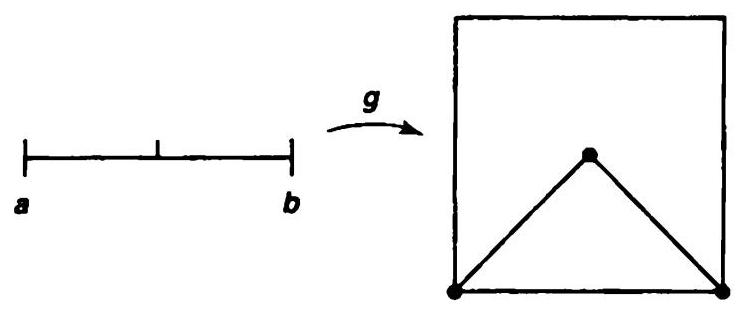
\includegraphics[width=0.6\textwidth]{images/44.1.jpg}
\end{center}
\hspace*{3em} 

Figure 44.1

\begin{center}
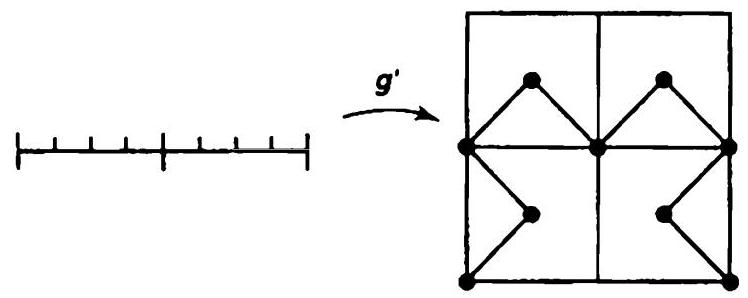
\includegraphics[width=0.6\textwidth]{images/44.2.jpg}
\end{center}
\hspace*{3em} 

Figure 44.2

This same operation can also be applied to any triangular path connecting two adjacent corners of the square. For instance, when applied to the path \(h\) pictured in Figure 443, it gives the path \({h}^{\prime }\)

Step 2. Now we define a sequence of functions \({f}_{n} : I \rightarrow  {I}^{2}\) . The first function, which we label \({f}_{0}\) for convenience, is the triangular path pictured in Figure 44.1, letting \(a = 0\) and \(b = 1\) . The next function \({f}_{1}\) is the function obtained by applying the operation described in Step 1 to the function \({f}_{0}\) ; it is pictured in Figure 44.2. The next function \({f}_{2}\) is the function obtained by applying this same operation to each of the four

\begin{center}
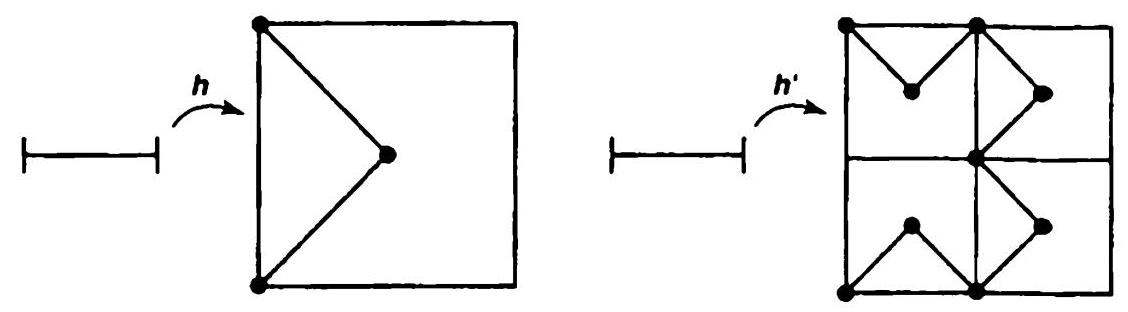
\includegraphics[width=1.0\textwidth]{images/44.3.jpg}
\end{center}
\hspace*{3em} 

Figure 44.3

triangular paths that make up \({f}_{1}\) . It is pictured in Figure 44.4. The next function \({f}_{3}\) is obtained by applying the operation to each of the 16 triangular paths that make up \({f}_{2}\) ; it is pictured in Figure 44.5. And so on. At the general step, \({f}_{n}\) is a path made up of \({4}^{n}\) triangular paths of the type considered in Step 1, each lying in a square of edge length \(1/{2}^{n}\) . The function \({f}_{n + 1}\) is obtained by applying the operation of Step1 to these triangular paths, replacing each one by four smaller triangular paths.

\begin{center}
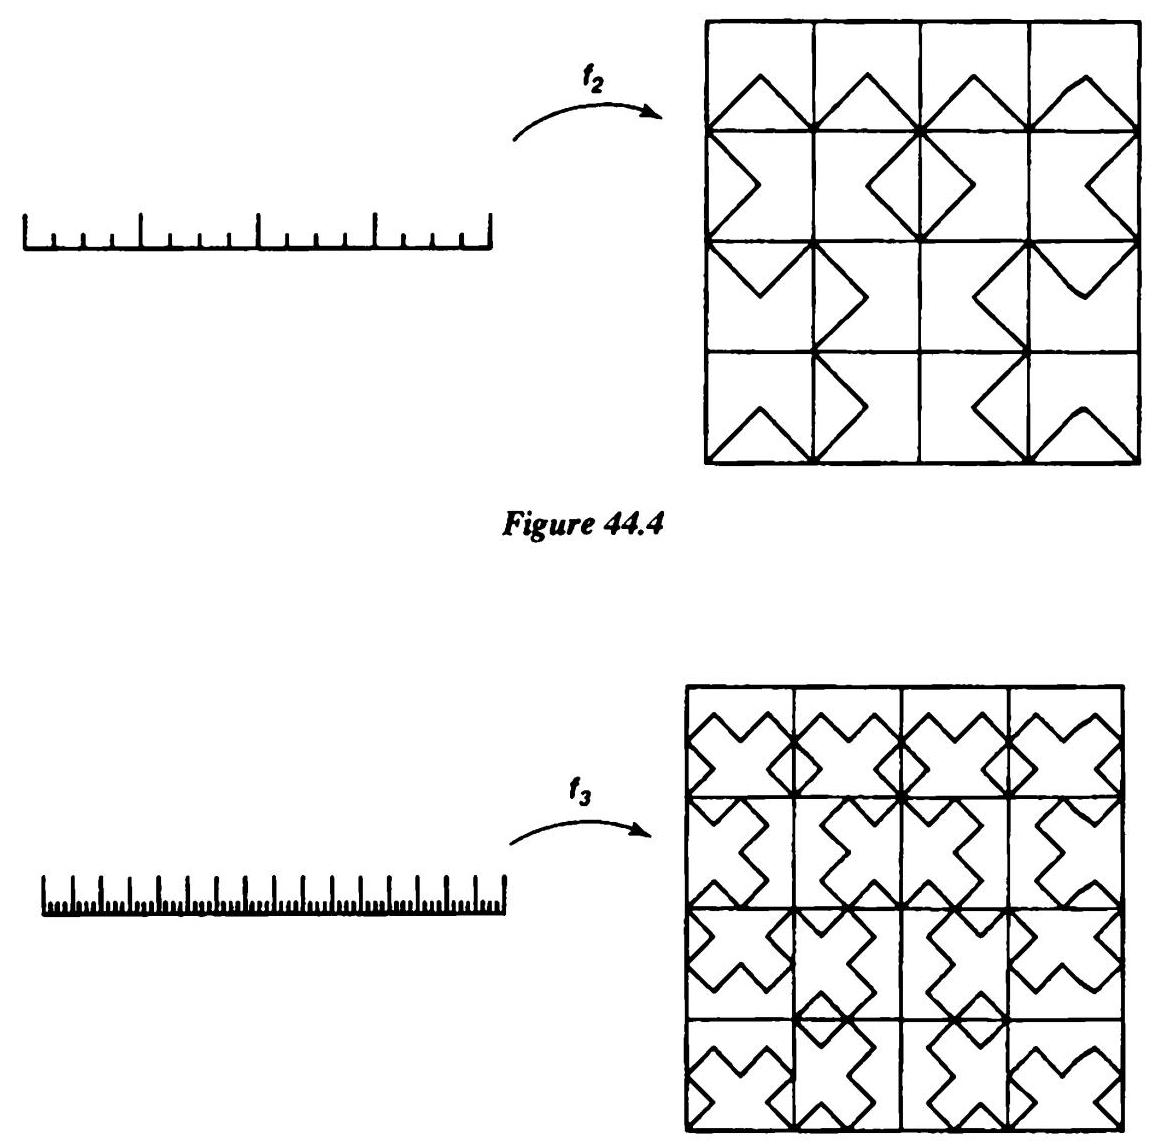
\includegraphics[width=1.0\textwidth]{images/44.4.jpg}
\end{center}
\hspace*{3em} 

Figure 44.5

Step 3. For purposes of this proof, let \(d\left( {\mathbf{x},\mathbf{y}}\right)\) denote the square metric on \({\mathbb{R}}^{2}\) ,

\[
d\left( {\mathbf{x},\mathbf{y}}\right)  = \max \left\{  {\left| {{x}_{1} - {y}_{1}}\right| ,\left| {{x}_{2} - {y}_{2}}\right| }\right\}  .
\]

Then we can let \(\rho\) denote the corresponding sup metric on \(\mathcal{C}\left( {I,{I}^{2}}\right)\) :

\[
\rho \left( {f,g}\right)  = \sup \{ d\left( {f\left( t\right) ,g\left( t\right) }\right)  \mid  t \in  I\} .
\]

Because \({I}^{2}\) is closed in \({\mathbb{R}}^{2}\) , it is complete in the square metric; then \(\mathcal{C}\left( {I,{I}^{2}}\right)\) is complete in the metric \(\rho\) .

We assert that the sequence of functions \(\left( {f}_{n}\right)\) defined in Step 2 is a Cauchy sequence under \(\rho\) . To prove this fact, let us examine what happens when we pass from \({f}_{n}\) to \({f}_{n + 1}\) . Each of the small triangular paths that make up \({f}_{n}\) lies in a square of edge length \(1/{2}^{n}\) . The operation by which we obtain \({f}_{n + 1}\) replaces each such triangular path by four triangular paths that lie in the same square. Therefore, in the square metric on \({I}^{2}\) , the distance between \({f}_{n}\left( t\right)\) and \({f}_{n + 1}\left( t\right)\) is at most \(1/{2}^{n}\) . As a result, \(\rho \left( {{f}_{n},{f}_{n + 1}}\right)  \leq  1/{2}^{n}\) . It follows that \(\left( {f}_{n}\right)\) is a Cauchy sequence, since

\[
\rho \left( {{f}_{n},{f}_{n + m}}\right)  \leq  1/{2}^{n} + 1/{2}^{n + 1} + \cdots  + 1/{2}^{n + m - 1} < 2/{2}^{n}
\]

for all \(n\) and \(m\) .

Step 4. Because \(\mathcal{C}\left( {I,{I}^{2}}\right)\) is complete, the sequence \({f}_{n}\) converges to a continuous function \(f : I \rightarrow  {I}^{2}\) . We prove that \(f\) is surjective.

Let \(x\) be a point of \({I}^{2}\) ; we show that \(x\) belongs to \(f\left( I\right)\) . First we note that, given \(n\) , the path \({f}_{n}\) comes within a distance of \(1/{2}^{n}\) of the point \(\mathbf{x}\) . For the path \({f}_{n}\) touches each of the little squares of edge length \(1/{2}^{n}\) into which we have divided \({I}^{2}\) .

Using this fact, we shall prove that, given \(\epsilon  > 0\) , the \(\epsilon\) -neighborhood of \(\mathbf{x}\) intersects \(f\left( I\right)\) . Choose \(N\) large enough that

\[
\rho \left( {{f}_{N},f}\right)  < \epsilon /2\;\text{ and }\;1/{2}^{N} < \epsilon /2.
\]

By the result of the previous paragraph, there is a point \({t}_{0} \in  I\) such that \(d\left( {\mathbf{x},{f}_{N}\left( {t}_{0}\right) }\right)  \leq\)  \(1/{2}^{N}\) . Then since \(d\left( {{f}_{N}\left( t\right) ,f\left( t\right) }\right)  < \epsilon /2\) for all \(t\) , it follows that

\[
d\left( {\mathbf{x},f\left( {t}_{0}\right) }\right)  < \epsilon ,
\]

so the \(\epsilon\) -neighborhood of \(\mathbf{x}\) intersects \(f\left( I\right)\) .

It follows that \(\mathbf{x}\) belongs to the closure of \(f\left( I\right)\) . But \(I\) is compact, so \(f\left( I\right)\) is compact and is therefore closed. Hence \(\mathbf{x}\) lies in \(f\left( I\right)\) , as desired.
\end{proof}
\section*{Exercises}

1. Given \(n\) , show there is a continuous surjective map \(g : I \rightarrow  {I}^{n}\) . [Hint: Consider \(\left. {f \times  f \cdot  I \times  I \rightarrow  {I}^{2} \times  {I}^{2}.}\right\rbrack\)

2. Show there is a continuous surjective map \(f : \mathbb{R} \rightarrow  {\mathbb{R}}^{n}\) .

3. (a) If \({\mathbb{R}}^{\omega }\) is given the product topology, show there is no continuous surjective map \(f : \mathbb{R} \rightarrow  {\mathbb{R}}^{\omega }\) . [Hint: Show that \({\mathbb{R}}^{\omega }\) is not a countable union of compact subspaces.]

(b) If \({\mathbb{R}}^{\omega }\) is given the product topology, determine whether or not there is a continuous surjective map of \(\mathbb{R}\) onto the subspace \({\mathbb{R}}^{\infty }\) .

(c) What happens to the statements in (a) and (b) if \({\mathbb{R}}^{\omega }\) is given the uniform topology or the box topology?

4. (a) Let \(X\) be a Hausdorff space. Show that if there is a continuous surjective map \(f : I \rightarrow  X\) , then \(X\) is compact, connected, weakly locally connected, and metrizable. [Hint: Show \(f\) is a perfect map.]

(b) The converse of the result in (a) is a famous theorem of point-set topology called the \idx{Hahn-Mazurkiewicz theorem} (see 		\cite{HockingYoung1961}, p. 129). Assuming this theorem, show there is a continuous surjective map \(f \cdot  I \rightarrow  {I}^{\omega }\) .

A Hausdorff space that is the continuous image of the closed unit interval is often called a \idx{Peano space} Peano space.

\section*{§ 45 Compactness in Metric Spaces}

We have already shown that compactness, limit point compactness, and sequential compactness are equivalent for metric spaces. There is still another formulation of compactness for metric spaces, one that involves the notion of completeness. We study it in this section. As an application, we shall prove a theorem characterizing those subspaces of \(\mathcal{C}\left( {X,{\mathbb{R}}^{n}}\right)\) that are compact in the uniform topology.

How is compactness of a metric space \(X\) related to completeness of \(X\) ? It follows from Lemma 431 that every compact metric space is complete. The converse does not hold-a complete metric space need not be compact. It is reasonable to ask what extra condition one needs to impose on a complete space to be assured of its compactness. Such a condition is the one called total boundedness.

\begin{definition} A metric space(X, d)is said to be \idx{totally bounded} if for every \(\epsilon  > 0\) , there is a finite covering of \(X\) by \(\epsilon\) -balls.
\end{definition}

\begin{example} Total boundedness clearly implies boundedness. For if \(B\left( {{x}_{1},1/2}\right) ,\ldots\) , \(B\left( {{x}_{n},1/2}\right)\) is a finite covering of \(X\) by open balls of radius \(1/2\) , then \(X\) has diameter at most \(1 + \max \left\{  {d\left( {{x}_{i},{x}_{j}}\right) }\right\}\) . The converse does not hold, however. For example, in the metric \(\bar{d}\left( {a,b}\right)  = \min \{ 1,\left| {a - b}\right| \}\) , the real line \(\mathbb{R}\) is bounded but not totally bounded.
\end{example}

\begin{example} Under the metric \(d\left( {a,b}\right)  = \left| {a - b}\right|\) , the real line \(\mathbb{R}\) is complete but not totally bounded, while the subspace(-1,1)is totally bounded but not complete. The subspace \(\left\lbrack  {-1,1}\right\rbrack\) is both complete and totally bounded.
\end{example}

\begin{theorem} A metric space(X, d)is compact if and only if it is complete and totally bounded.
\end{theorem}

\begin{proof}If \(X\) is a compact metric space, then \(X\) is complete, as noted above. The fact that \(X\) is totally bounded is a consequence of the fact that the covering of \(X\) by all open \(\epsilon\) -balls must contain a finite subcovering.
Conversely, let \(X\) be complete and totally bounded. We shall prove that \(X\) is sequentially compact. This will suffice.

Let \(\left( {x}_{n}\right)\) be a sequence of points of \(X\) . We shall construct a subsequence of \(\left( {x}_{n}\right)\) that is a Cauchy sequence, so that it necessarily converges. First cover \(X\) by finitely many balls of radius 1 . At least one of these balls, say \({B}_{1}\) , contains \({x}_{n}\) for infinitely many values of \(n\) . Let \({J}_{1}\) be the subset of \({\mathbb{Z}}_{ + }\) consisting of those indices \(n\) for which \({x}_{n} \in  {B}_{1}\) .

Next, cover \(X\) by finitely many balls of radius \(1/2\) . Because \({J}_{1}\) is infinite, at least one of these balls, say \({B}_{2}\) , must contain \({x}_{n}\) for infinitely many values of \(n\) in \({J}_{1}\) . Choose \({J}_{2}\) to be the set of those indices \(n\) for which \(n \in  {J}_{1}\) and \({x}_{n} \in  {B}_{2}\) . In general, given an infinite set \({J}_{k}\) of positive integers, choose \({J}_{k + 1}\) to be an infinite subset of \({J}_{k}\) such that there is a ball \({B}_{k + 1}\) of radius \(1/\left( {k + 1}\right)\) that contains \({x}_{n}\) for all \(n \in  {J}_{k + 1}\) .

Choose \({n}_{1} \in  {J}_{1}\) . Given \({n}_{k}\) , choose \({n}_{k + 1} \in  {J}_{k + 1}\) such that \({n}_{k + 1} > {n}_{k}\) ; this we can do because \({J}_{k + 1}\) is an infinite set. Now for \(i,j \geq  k\) , the indices \({n}_{i}\) and \({n}_{j}\) both belong to \({J}_{k}\) (because \({J}_{1} \supset  {J}_{2} \supset  \cdots\) is a nested sequence of sets). Therefore, for all \(i,j \geq  k\) , the points \({x}_{{n}_{i}}\) and \({x}_{{n}_{j}}\) are contained in a ball \({B}_{k}\) of radius \(1/k\) . It follows that the sequence \(\left( {x}_{{n}_{1}}\right)\) is a Cauchy sequence, as desired.

We now apply this result to find the compact subspaces of the space \(\mathcal{C}\left( {X,{\mathbb{R}}^{n}}\right)\) , in the uniform topology. We know that a subspace of \({\mathbb{R}}^{n}\) is compact if and only if it is closed and bounded. One might hope that an analogous result holds for \(\mathcal{C}\left( {X,{\mathbb{R}}^{n}}\right)\) . But it does not, even if \(X\) is compact. One needs to assume that the subspace of \(\mathcal{C}\left( {X,{\mathbb{R}}^{n}}\right)\) satisfies an additional condition, called \idx{equicontinuity}. We consider that notion now.
\end{proof}
\begin{definition} Let(Y, d)be a metric space. Let \(\mathcal{F}\) be a subset of the function space \(\mathcal{C}\left( {X,Y}\right)\) . If \({x}_{0} \in  X\) , the set \(\mathcal{F}\) of functions is said to be equicontinuous at \({x}_{0}\) if given \(\epsilon  > 0\) , there is a neighborhood \(U\) of \({x}_{0}\) such that for all \(x \in  U\) and all \(f \in  \mathcal{F}\) ,

\[
d\left( {f\left( x\right) ,f\left( {x}_{0}\right) }\right)  < \epsilon
\]

If the set \(\mathcal{F}\) is equicontinuous at \({x}_{0}\) for each \({x}_{0} \in  X\) , it is said simply to be equicontinuous.
\end{definition}

Continuity of the function \(f\) at \({x}_{0}\) means that given \(f\) and given \(\epsilon  > 0\) , there exists a neighborhood \(U\) of \({x}_{0}\) such that \(d\left( {f\left( x\right) ,f\left( {x}_{0}\right) }\right)  < \epsilon\) for \(x \in  U\) . Equicontinuity of \(\mathcal{F}\) means that a single neighborhood \(U\) can be chosen that will work for all the functions \(f\) in the collection \(\mathcal{F}\) .

Note that equicontinuity depends on the specific metric \(d\) rather than merely on the topology of \(Y\) .

\begin{lemma} Let \(X\) be a space; let(Y, d)be a metric space. If the subset \(\mathcal{F}\) of \(\mathcal{C}\left( {X,Y}\right)\) is totally bounded under the uniform metric corresponding to \(d\) , then \(\mathcal{F}\) is equicontinuous under \(d\) .
\end{lemma}

\begin{proof}Assume \(\mathcal{F}\) is totally bounded. Given \(0 < \epsilon  < 1\) , and given \({x}_{0}\) , we find a neighborhood \(U\) of \({x}_{0}\) such that \(d\left( {f\left( x\right) ,f\left( {x}_{0}\right)  < \epsilon }\right.\) for \(x \in  U\) and \(f \in  \mathcal{F}\) .
Set \(\delta  = \epsilon /3\) ; cover \(\mathcal{F}\) by finitely many open \(\delta\) -balls

\[
B\left( {{f}_{1},\delta }\right) ,\ldots ,B\left( {{f}_{n},\delta }\right)
\]

in \(\mathcal{C}\left( {X,Y}\right)\) . Each function \({f}_{i}\) is continuous; therefore, we can choose a neighborhood \(U\) of \({x}_{0}\) such that for \(i = 1,\ldots ,n\) ,

\[
d\left( {{f}_{i}\left( x\right) ,{f}_{i}\left( {x}_{0}\right) }\right)  < \delta
\]

whenever \(x \in  U\) .

Let \(f\) be an arbitrary element of \(\mathcal{F}\) . Then \(f\) belongs to at least one of the above \(\delta\) -balls, say to \(B\left( {{f}_{i},\delta }\right)\) . Then for \(x \in  U\) , we have

\[
\bar{d}\left( {f\left( x\right) ,{f}_{i}\left( x\right) }\right)  < \delta ,
\]

\[
d\left( {{f}_{i}\left( x\right) ,{f}_{i}\left( {x}_{0}\right) }\right)  < \delta ,
\]

\[
\bar{d}\left( {{f}_{i}\left( {x}_{0}\right) ,f\left( {x}_{0}\right) }\right)  < \delta .
\]

The first and third inequalities hold because \(\bar{\rho }\left( {f,{f}_{i}}\right)  < \delta\) , and the second holds because \(x \in  U\) . Since \(\delta  < 1\) , the first and third also hold if \(\bar{d}\) is replaced by \(d\) ; then the triangle inequality implies that for all \(x \in  U\) , we have \(d\left( {f\left( x\right) ,f\left( {x}_{0}\right) }\right)  < \epsilon\) , as desired.

Now we prove the classical version of \idx{Ascoli's theorem}, which concerns compact subspaces of the function space \(\mathcal{C}\left( {X,{\mathbb{R}}^{n}}\right)\) . A more general version, whose proof does not depend on this one, is given in §47. The general version, however, relies on the Tychonoff theorem, whereas this one does not.

We begin by proving a partial converse to the preceding lemma, which holds when \(X\) and \(Y\) are compact.

*Lemma 45.3. Let \(X\) be a space; let(Y, d)be a metric space; assume \(X\) and \(Y\) are compact. If the subset \(\mathcal{F}\) of \(\mathcal{C}\left( {X,Y}\right)\) is equicontinuous under \(d\) , then \(\mathcal{F}\) is totally bounded under the uniform and sup metrics corresponding to \(d\) .

Proof. Since \(X\) is compact, the sup metric \(\rho\) is defined on \(\mathcal{C}\left( {X,Y}\right)\) . Total boundedness under \(\rho\) is equivalent to total boundedness under \(\bar{\rho }\) , for whenever \(\epsilon  < 1\) , every \(\epsilon\) -ball under \(\rho\) is also an \(\epsilon\) -ball under \(\bar{\rho }\) , and conversely. Therefore, we may as well use the metric \(\rho\) throughout.

Assume \(\mathcal{F}\) is equicontinuous. Given \(\epsilon  > 0\) , we cover \(\mathcal{F}\) by finitely many sets that are open \(\epsilon\) -balls in the metric \(\rho\) .

Set \(\delta  = \epsilon /3\) . Given any \(a \in  X\) , there is a corresponding neighborhood \({U}_{a}\) of \(a\) such that \(d\left( {f\left( x\right) ,f\left( a\right) }\right)  < \delta\) for all \(x \in  {U}_{a}\) and all \(f \in  \mathcal{F}\) . Cover \(X\) by finitely many such neighborhoods \({U}_{a}\) , for \(a = {a}_{1},\ldots ,{a}_{k}\) , denote \({U}_{{a}_{i}}\) by \({U}_{i}\) . Then cover \(Y\) by finitely many open sets \({V}_{1},\ldots ,{V}_{m}\) of diameter less than \(\delta\) .

Let \(J\) be the collection of all functions \(\alpha  : \{ 1,\ldots ,k\}  \rightarrow  \{ 1,\ldots ,m\}\) . Given \(\alpha  \in  J\) , if there exists a function \(f\) of \(\mathcal{F}\) such that \(f\left( {a}_{i}\right)  \in  {V}_{\alpha \left( i\right) }\) for each \(i = 1,\ldots ,k\) , choose one such function and label it \({f}_{\alpha }\) . The collection \(\left\{  {f}_{\alpha }\right\}\) is indexed by a subset \({J}^{\prime }\) of the set \(J\) and is thus finite We assert that the open balls \({B}_{\rho }\left( {{f}_{\alpha },\epsilon }\right)\) , for \(\alpha  \in  {J}^{\prime }\) , cover \(\mathcal{F}\) .

Let \(f\) be an element of \(\mathcal{F}\) . For each \(i = 1,\ldots ,k\) , choose an integer \(\alpha \left( i\right)\) such that \(f\left( {a}_{i}\right)  \in  {V}_{\alpha \left( i\right) }\) . Then the function \(\alpha\) is in \({J}^{\prime }\) . We assert that \(f\) belongs to the ball \({B}_{\rho }\left( {{f}_{\alpha },\epsilon }\right)\) .

Let \(x\) be a point of \(X\) . Choose \(i\) so that \(x \in  {U}_{i}\) . Then

\[
d\left( {f\left( x\right) ,f\left( {a}_{l}\right) }\right)  < \delta ,
\]

\[
d\left( {f\left( {a}_{i}\right) ,{f}_{\alpha }\left( {a}_{i}\right) }\right)  < \delta ,
\]

\[
d\left( {{f}_{\alpha }\left( {a}_{i}\right) ,{f}_{\alpha }\left( x\right) }\right)  < \delta .
\]

The first and third inequalities hold because \(x \in  {U}_{i}\) , and the second holds because \(f\left( {a}_{i}\right)\) and \({f}_{\alpha }\left( {a}_{i}\right)\) are in \({V}_{\alpha \left( i\right) }\) . We conclude that \(d\left( {f\left( x\right) ,{f}_{\alpha }\left( x\right) }\right)  < \epsilon\) . Because this inequality holds for every \(x \in  X\) ,

\[
\rho \left( {f,{f}_{\alpha }}\right)  = \max \left\{  {d\left( {f\left( x\right) ,{f}_{\alpha }\left( x\right) }\right) }\right\}   < \epsilon .
\]

Thus \(f\) belongs to \({B}_{\rho }\left( {{f}_{\alpha },\epsilon }\right)\) , as asserted.
\end{proof}
\begin{definition} If(Y, d)is a metric space, a subset \(\mathcal{F}\) of \(\mathcal{C}\left( {X,Y}\right)\) is said to be \idx{pointwise bounded} under \(d\) if for each \(x \in  X\) , the subset

\[
{\mathcal{F}}_{a} = \{ f\left( a\right)  \mid  f \in  \mathcal{F}\}
\]

of \(Y\) is bounded under \(d\) .
\end{definition}

*Theorem 45.4 (Ascoli’s theorem, classical version). Let \(X\) be a compact space; let \(\left( {{\mathbb{R}}^{n},d}\right)\) denote euclidean space in either the square metric or the euclidean metric; give \(\mathcal{C}\left( {X,{\mathbb{R}}^{n}}\right)\) the corresponding uniform topology. A subspace \(\mathcal{F}\) of \(\mathcal{C}\left( {X,{\mathbb{R}}^{n}}\right)\) has compact closure if and only if \(\mathcal{F}\) is equicontinuous and pointwise bounded under \(d\) .

\begin{proof}Since \(X\) is compact, the sup metric \(\rho\) is defined on \(\mathcal{C}\left( {X,{\mathbb{R}}^{n}}\right)\) and gives the uniform topology on \(\mathcal{C}\left( {X,{\mathbb{R}}^{n}}\right)\) . Throughout, let \(\mathcal{G}\) denote the closure of \(\mathcal{F}\) in \(C\left( {X,{\mathbb{R}}^{n}}\right)\) .
Step 1. We show that if \(g\) is compact, then \(g\) is equicontinuous and pointwise bounded under \(d\) . Since \(\mathcal{F} \subset  \mathcal{G}\) , it follows that \(\mathcal{F}\) is also equicontinuous and pointwise bounded under \(d\) . This proves the "only if" part of the theorem.

Compactness of \(\mathcal{G}\) implies that \(\mathcal{G}\) is totally bounded under \(\rho\) and \(\bar{\rho }\) by Theorem 45.1, this in turn implies that \(\mathcal{G}\) is equicontinuous under \(d\) , by Lemma 45.2. Compactness of \(\mathcal{G}\) also implies that \(\mathcal{G}\) is bounded under \(\rho\) ; this in turn implies that \(\mathcal{G}\) is pointwise bounded under \(d\) . For if \(\rho \left( {f,g}\right)  \leq  M\) for all \(f,g \in  \mathcal{G}\) , then in particular \(d\left( {f\left( a\right) ,g\left( a\right) }\right)  \leq  M\) for \(f,g \in  \mathcal{G}\) , so that \({\mathcal{G}}_{a}\) has diameter at most \(M\) .

Step 2. We show that if \(\mathcal{F}\) is equicontinuous and pointwise bounded under \(d\) , then so is \(g\) .

First, we check equicontinuity. Given \({x}_{0} \in  X\) and given \(\epsilon  > 0\) , choose a neighborhood \(U\) of \({x}_{0}\) such that \(d\left( {f\left( x\right) ,f\left( {x}_{0}\right) }\right)  < \epsilon /3\) for all \(x \in  U\) and \(f \in  \mathcal{F}\) . Given \(g \in  \mathcal{G}\) , choose \(f \in  \mathcal{F}\) so that \(\rho \left( {f,g}\right)  < \epsilon /3\) The triangle inequality implies that \(d\left( {g\left( x\right) ,g\left( {x}_{0}\right) }\right)  < \epsilon\) for all \(x \in  U\) . Since \(g\) is arbitrary, equicontinuity of \(\mathcal{G}\) at \({x}_{0}\) follows.

Second, we verify pointwise boundedness. Given \(a\) , choose \(M\) so that \(\operatorname{diam}{\mathcal{F}}_{a} \leq\)  \(M\) . Then, given \(g,{g}^{\prime } \in  \mathcal{G}\) , choose \(f,{f}^{\prime } \in  \mathcal{F}\) such that \(\rho \left( {f,g}\right)  < 1\) and \(\rho \left( {{f}^{\prime },{g}^{\prime }}\right)  < 1\) . Since \(d\left( {f\left( a\right) ,{f}^{\prime }\left( a\right) }\right)  \leq  M\) , it follows that \(d\left( {g\left( a\right) ,{g}^{\prime }\left( a\right) }\right)  \leq  M + 2\) . Then since \(g\) and \({g}^{\prime }\) are arbitrary, it follows that diam \({\mathcal{G}}_{a} \leq  M + 2\) .

Step 3. We show that if \(\xi\) is equicontinuous and pointwise bounded, then there is a compact subspace \(Y\) of \({\mathbb{R}}^{n}\) that contains the union of the sets \(g\left( X\right)\) , for \(g \in  \mathcal{G}\) .

Choose, for each \(a \in  X\) , a neighborhood \({U}_{a}\) of \(a\) such that \(d\left( {g\left( x\right) ,g\left( a\right) }\right)  < 1\) for \(x \in  {U}_{a}\) and \(g \in  \mathcal{G}\) . Since \(X\) is compact, we can cover \(X\) by finitely many such neighborhoods, say for \(a = {a}_{1},\ldots ,{a}_{k}\) . Because the sets \({\mathcal{G}}_{{a}_{i}}\) are bounded, their union is also bounded; suppose it lies in the ball of radius \(N\) in \({\mathbb{R}}^{n}\) centered at the origin. Then for all \(g \in  \mathcal{G}\) , the set \(g\left( X\right)\) is contained in the ball of radius \(N + 1\) centered at the origin. Let \(Y\) be the closure of this ball.

Step 4. We prove the "if" part of the theorem. Assume that \(\mathcal{F}\) is equicontinuous and pointwise bounded under \(d\) . We show that \(\mathcal{G}\) is complete and totally bounded under \(\rho\) ; then Theorem 45.1 implies that \(\mathcal{G}\) is compact.

Completeness is easy, for \(\mathcal{G}\) is a closed subspace of the complete metric space \(\left( {C\left( {X,{\mathbb{R}}^{n}}\right) ,\rho }\right)\) .

We verify total boundedness. First, Step 2 implies that \(\mathcal{G}\) is equicontinuous and pointwise bounded under \(d\) ; then Step 3 tells us that there is a compact subspace \(Y\) of \({\mathbb{R}}^{n}\) such that \(\mathcal{G} \subset  \mathcal{C}\left( {X,Y}\right)\) . Equicontinuity of \(\mathcal{G}\) now implies, by Lemma 45.3, that \(\mathcal{G}\) is totally bounded under \(\rho\) , as desired.

*Corollary 45.5. Let \(X\) be compact; let \(d\) denote either the square metric or the euclidean metric on \({\mathbb{R}}^{n}\) ; give \(\mathcal{C}\left( {X,{\mathbb{R}}^{n}}\right)\) the corresponding uniform topology. A subspace \(\mathcal{F}\) of \(\mathcal{C}\left( {X,{\mathbb{R}}^{n}}\right)\) is compact if and only if it is closed, bounded under the sup metric \(\rho\) , and equicontinuous under \(d\) .

Proof. If \(\mathcal{F}\) is compact, it must be closed and bounded; the preceding theorem implies that it is also equicontinuous. Conversely, if \(\mathcal{F}\) is closed, it equals its closure \(\mathcal{G}\) ; if it is bounded under \(\rho\) , it is pointwise bounded under \(d\) ; and if it is also equicontinuous, the preceding theorem implies that it is compact.
\end{proof}
\section*{Exercises}

1. If \({X}_{n}\) is metrizable with metric \({d}_{n}\) , then

\[
D\left( {\mathbf{x},\mathbf{y}}\right)  = \sup \left\{  {{\bar{d}}_{i}\left( {{x}_{i},{y}_{i}}\right) /i}\right\}
\]

is a metric for the product space \(X = \prod {X}_{n}\) . Show that \(X\) is totally bounded under \(D\) if each \({X}_{n}\) is totally bounded under \({d}_{n}\) . Conclude without using the Ty-chonoff theorem that a countable product of compact metrizable spaces is compact.

2. Let(Y, d)be a metric space; let \(\mathcal{F}\) be a subset of \(\mathcal{C}\left( {X,Y}\right)\) .

(a) Show that if \(\mathcal{F}\) is finite, then \(\mathcal{F}\) is equicontinuous.

(b) Show that if \({f}_{n}\) is a sequence of elements of \(\mathcal{C}\left( {X,Y}\right)\) that converges uniformly, then the collection \(\left\{  {f}_{n}\right\}\) is equicontinuous.

(c) Suppose that \(\mathcal{F}\) is a collection of differentiable functions \(f : \mathbb{R} \rightarrow  \mathbb{R}\) such that each \(x \in  \mathbb{R}\) lies in a neighborhood \(U\) on which the derivatives of the functions in \(\mathcal{F}\) are uniformly bounded. \{This means that there is an \(M\) such that \(\left| {{f}^{\prime }\left( x\right) }\right|  \leq  M\) for all \(f\) in \(\mathcal{F}\) and all \(x \in  U\) .] Show that \(\mathcal{F}\) is equicontinuous.

3. Prove the following:

\begin{theorem}[\idx{Arzela’s theorem} Arzela’s theorem] Let \(X\) be compact; let \({f}_{n} \in  \mathcal{C}\left( {X,{\mathbb{R}}^{k}}\right)\) . If the collection \(\left\{  {f}_{n}\right\}\) is pointwise bounded and equicontinuous, then the sequence \({f}_{n}\) has a uniformly convergent subsequence.
\end{theorem}

4. (a) Let \({f}_{n} : I \rightarrow  \mathbb{R}\) be the function \({f}_{n}\left( x\right)  = {x}^{n}\) . The collection \(\mathcal{F} = \left\{  {f}_{n}\right\}\) is pointwise bounded but the sequence \(\left( {f}_{n}\right)\) has no uniformly convergent subsequence; at what point or points does \(\mathcal{F}\) fail to be equicontinuous?

(b) Repeat (a) for the functions \({f}_{n}\) of Exercise 9 of \(§{21}\) .

5. Let \(X\) be a space. A subset \(\mathcal{F}\) of \(\mathcal{C}\left( {X,\mathbb{R}}\right)\) is said to vanish uniformly at infinity if given \(\epsilon  > 0\) , there is a compact subspace \(C\) of \(X\) such that \(\left| {f\left( x\right) }\right|  < \epsilon\) for \(x \in  X - C\) and \(f \in  \mathcal{F}\) If \(\mathcal{F}\) consists of a single function \(f\) , we say simply that \(f\) vanishes at infinity. Let \({\mathcal{C}}_{0}\left( {X,\mathbb{R}}\right)\) denote the set of continuous functions \(f : X \rightarrow  \mathbb{R}\) that \idx{vanish at infinity}.

\begin{theorem} Let \(X\) be locally compact Hausdorff; give \({\mathcal{C}}_{0}\left( {X,\mathbb{R}}\right)\) the uniform topology. A subset \(\mathcal{F}\) of \({\mathcal{C}}_{0}\left( {X,\mathbb{R}}\right)\) has compact closure if and only if it is pointwise bounded, equicontinuous, and vanishes uniformly at infinity.
\end{theorem}

\{Hint: Let \(Y\) denote the one-point compactification of \(X\) . Show that \({\mathcal{C}}_{0}\left( {X,\mathbb{R}}\right)\) is isometric with a closed subspace of \(\mathcal{C}\left( {Y,\mathbb{R}}\right)\) if both are given the sup metric.]

6. Show that our proof of Ascoli’s theorem goes through if \({\mathbb{R}}^{n}\) is replaced by any metric space in which all closed bounded subspaces are compact.

*7. Let(X, d)be a metric space. If \(A \subset  X\) and \(\epsilon  > 0\) , let \(U\left( {A,\epsilon }\right)\) be the \(\epsilon\) - neighborhood of \(A\) . Let \(\mathcal{H}\) be the collection of all (nonempty) closed, bounded subsets of \(X\) . If \(A,B \in  \mathcal{H}\) , define

\[
D\left( {A,B}\right)  = \inf \{ \epsilon  \mid  A \subset  U\left( {B,\epsilon }\right) \text{ and }B \subset  U\left( {A,\epsilon }\right) \} .
\]

(a) Show that \(D\) is a metric on \(\mathcal{H}\) ; it is called the \idx{Hausdorff metric}.

(b) Show that if(X, d)is complete, so is(H, D). [Hint: Let \({A}_{n}\) be a Cauchy sequence in \(\mathcal{H}\) ; by passing to a subsequence, assume \(D\left( {{A}_{n},{A}_{n + 1}}\right)  < 1/{2}^{n}\) . Define \(A\) to be the set of all points \(x\) that are the limits of sequences \({x}_{1},{x}_{2}\) , ... such that \({x}_{i} \in  {A}_{i}\) for each \(i\) and \(d\left( {{x}_{i},{x}_{i + 1}}\right)  < 1/{2}^{i}\) . Show \(\left. {{A}_{n} \rightarrow  \bar{A}\text{ . }}\right\rbrack\)

(c) Show that if(X, d)is totally bounded, so is(H, D). [Hint: Given \(\epsilon\) , choose \(\delta  < \epsilon\) and let \(S\) be a finite subset of \(X\) such that the collection \(\left\{  {{B}_{d}\left( {x,\delta }\right)  \mid  }\right.\)  \(x \in  S\}\) covers \(X\) . Let \(\mathcal{A}\) be the collection of all nonempty subsets of \(S\) ; show that \(\left\{  {{B}_{D}\left( {A,\epsilon }\right)  \mid  A \in  \mathcal{A}}\right\}\) covers \(\mathcal{H}\) .]

(d) Theorem. If \(X\) is compact in the metric \(d\) , then the space \(\mathcal{H}\) is compact in the Hausdorff metric \(D\) .

*8. Let \(\left( {X,{d}_{X}}\right)\) and \(\left( {Y,{d}_{Y}}\right)\) be metric spaces; give \(X \times  Y\) the corresponding square metric; let \(\mathcal{H}\) denote the collection of all nonempty closed, bounded subsets of \(X \times  Y\) in the resulting Hausdorff metric. Consider the space \(\mathcal{C}\left( {X,Y}\right)\) in the uniform metric; let \(\operatorname{gr} : \mathcal{C}\left( {X,Y}\right)  \rightarrow  \mathcal{H}\) be the function that assigns, to each continuous function \(f : X \rightarrow  Y\) , its graph

\[
{G}_{f} = \{ x \times  f\left( x\right)  \mid  x \in  X\} .
\]

(a) Show that the map gr is injective and uniformly continuous.

(b) Let \({\mathcal{H}}_{0}\) denote the image set of the map gr; let \(g : \mathcal{C}\left( {X,Y}\right)  \rightarrow  {\mathcal{H}}_{0}\) be the surjective map obtained from gr. Show that if \(f : X \rightarrow  Y\) is uniformly continuous, then the map \({g}^{-1}\) is continuous at the point \({G}_{f}\) .

(c) Give an example where \({g}^{-1}\) is not continuous at the point \({G}_{f}\) .

(d) Theorem. If \(X\) is compact, then \(\operatorname{gr} : \mathcal{C}\left( {X,Y}\right)  \rightarrow  \mathcal{H}\) is an imbedding.

\section*{§ 46 Pointwise and Compact Convergence}

There are other useful topologies on the spaces \({Y}^{X}\) and \(\mathcal{C}\left( {X,Y}\right)\) in addition to the uniform topology. We shall consider three of them here; they are called the topology of pointwise convergence, the topology of compact convergence, and the \idx{compact-open topology}.

\begin{definition} Given a point \(x\) of the set \(X\) and an open set \(U\) of the space \(Y\) , let

\[
S\left( {x,U}\right)  = \left\{  {f \mid  f \in  {Y}^{\chi }\text{ and }f\left( x\right)  \in  U}\right\}  .
\]

The sets \(S\left( {x,U}\right)\) are a subbasis for topology on \({Y}^{X}\) , which is called the topology of pointwise convergence (or the \idx{point-open topology}).
\end{definition}

The general basis element for this topology is a finite intersection of subbasis elements \(S\left( {x,U}\right)\) . Thus a typical basis element about the function \(f\) consists of all functions \(g\) that are "close" to \(f\) at finitely many points. Such a neighborhood is illustrated in Figure 46.1; it consists of all functions \(g\) whose graphs intersect the three vertical intervals pictured.

\begin{center}
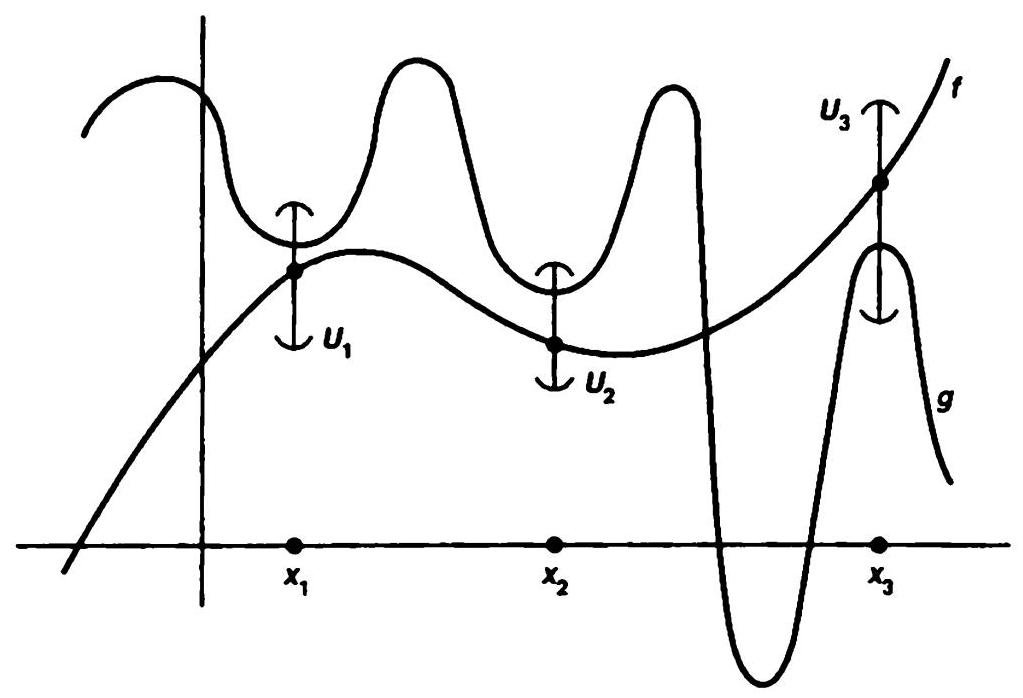
\includegraphics[width=0.9\textwidth]{images/46.1.jpg}
\end{center}
\hspace*{3em} 

Figure 46.1

The topology of pointwise convergence on \({Y}^{X}\) is nothing new. It is just the product topology we have already studied. If we replace \(X\) by \(J\) and denote the general element of \(J\) by \(\alpha\) to make it look more familiar, then the set \(S\left( {\alpha ,U}\right)\) of all functions \(\mathbf{x} : J \rightarrow  Y\) such that \(\mathbf{x}\left( \alpha \right)  \in  U\) is just the subset \({\pi }_{\alpha }^{-1}\left( U\right)\) of \({Y}^{J}\) , which is the standard subbasis element for the product topology.

The reason for calling it the topology of pointwise convergence comes from the following theorem:

\begin{theorem} A sequence \({f}_{n}\) of functions converges to the function \(f\) in the topology of pointwise convergence if and only if for each \(x\) in \(X\) , the sequence \({f}_{n}\left( x\right)\) of points of \(Y\) converges to the point \(f\left( x\right)\) .
\end{theorem}

\begin{proof}This result is just a reformulation, in function space notation, of a standard result about the product topology proved as Lemma 43.3.
\begin{example} Consider the space \({\mathbb{R}}^{I}\) , where \(I = \left\lbrack  {0,1}\right\rbrack\) . The sequence \(\left( {f}_{n}\right)\) of continuous functions given by \({f}_{n}\left( x\right)  = {x}^{n}\) converges in the topology of pointwise convergence to the function \(f\) defined by

\[
f\left( x\right)  = \left\{  \begin{array}{ll} 0 & \text{ for }0 \leq  x < 1 \\  1 & \text{ for }x = 1 \end{array}\right.
\]
\end{example}

This example shows that the subspace \(\mathcal{C}\left( {I,\mathbb{R}}\right)\) of continuous functions is not closed in \({\mathbb{R}}^{I}\) in the topology of pointwise convergence.

We know that a sequence \(\left( {f}_{n}\right)\) of continuous functions that converges in the uniform topology has a continuous limit, and the preceding example shows that a sequence that converges only in the topology of pointwise convergence need not. One can ask whether there is a topology intermediate between these two that will suffice to ensure that the limit of a convergent sequence of continuous functions is continuous. The answer is "yes", assuming the (fairly mild) restriction that the space \(X\) be compactly generated, it will suffice if \({f}_{n}\) converges to \(f\) in the topology of compact convergence, which we now define.
\end{proof}
\begin{definition} Let(Y, d)be a metric space; let \(X\) be a topological space. Given an element \(f\) of \({Y}^{X}\) , a compact subspace \(C\) of \(X\) , and a number \(\epsilon  > 0\) , let \({B}_{C}\left( {f,\epsilon }\right)\) denote the set of all those elements \(g\) of \({Y}^{X}\) for which

\[
\sup \{ d\left( {f\left( x\right) ,g\left( x\right) }\right)  \mid  x \in  C\}  < \epsilon .
\]

The sets \({B}_{C}\left( {f,\epsilon }\right)\) form a basis for a topology on \({Y}^{X}\) . It is called the topology of compact convergence (or sometimes the "topology of uniform convergence on compact sets").
\end{definition}

It is easy to show that the sets \({B}_{C}\left( {f,\epsilon }\right)\) satisfy the conditions for a basis. The crucial step is to note that if \(g \in  {B}_{C}\left( {f,\epsilon }\right)\) , then for

\[
\delta  = \epsilon  - \sup \{ d\left( {f\left( x\right) ,g\left( x\right) }\right)  \mid  x \in  C\} .
\]

we have \({B}_{C}\left( {g,\delta }\right)  \subset  {B}_{C}\left( {f,\epsilon }\right)\) .

The topology of compact convergence differs from the topology of pointwise convergence in that the general basis element containing \(f\) consists of functions that are "close" to \(f\) not just at finitely many points, but at all points of some compact set.

The justification for the choice of terminology comes from the following theorem, whose proof is immediate.

\begin{theorem} A sequence \({f}_{n}\;X \rightarrow  Y\) of functions converges to the function \(f\) in the topology of compact convergence if and only if for each compact subspace \(C\) of \(X\) , the sequence \({f}_{n} \mid  C\) converges uniformly to \(f \mid  C\) .
\end{theorem}

\begin{definition} A space \(X\) is said to be compactly generated if it satisfies the following condition: A set \(A\) is open in \(X\) if \(A \cap  C\) is open in \(C\) for each compact subspace \(C\) of \(X\) .
\end{definition}

This condition is equivalent to requiring that a set \(B\) be closed in \(X\) if \(B \cap  C\) is closed in \(C\) for each compact \(C\) . It is a fairly mild restriction on the space; many familiar spaces are compactly generated. For instance:

Lemma 46.3. If \(X\) is locally compact, or if \(X\) satisfies the first countability axiom, then \(X\) is compactly generated. Proof. Suppose that \(X\) is locally compact. Let \(A \cap  C\) be open in \(C\) for every compact subspace \(C\) of \(X\) . We show \(A\) is open in \(X\) . Given \(x \in  A\) , choose a neighborhood \(U\) of \(x\) that lies in a compact subspace \(C\) of \(X\) . Since \(A \cap  C\) is open in \(C\) by hypothesis, \(A \cap  U\) is open in \(U\) , and hence open in \(X\) . Then \(A \cap  U\) is a neighborhood of \(x\) contained in \(A\) , so that \(A\) is open in \(X\) .

Suppose that \(X\) satisfies the first countability axiom. If \(B \cap  C\) is closed in \(C\) for each compact subspace \(C\) of \(X\) , we show that \(B\) is closed in \(X\) . Let \(x\) be a point of \(\bar{B}\) ; we show that \(x \in  B\) . Since \(X\) has a countable basis at \(x\) , there is a sequence \(\left( {x}_{n}\right)\) of points of \(B\) converging to \(x\) . The subspace

\[
C = \{ x\}  \cup  \left\{  {{x}_{n} \mid  n \in  {\mathbb{Z}}_{ + }}\right\}
\]

is compact, so that \(B \cap  C\) is by assumption closed in \(C\) . Since \(B \cap  C\) contains \({x}_{n}\) for every \(n\) , it contains \(x\) as well. Therefore, \(x \in  B\) , as desired.

The crucial fact about \idx{compactly generated space}s is the following:

\begin{lemma} If \(X\) is compactly generated, then a function \(f : X \rightarrow  Y\) is continuous if for each compact subspace \(C\) of \(X\) , the restricted function \(f \mid  C\) is continuous.
\end{lemma}

\begin{proof}Let \(V\) be an open subset of \(Y\) ; we show that \({f}^{-1}\left( V\right)\) is open in \(X\) . Given any subspace \(C\) of \(X\) ,
\[
{f}^{-1}\left( V\right)  \cap  C = {\left( f \mid  C\right) }^{-1}\left( V\right) .
\]

If \(C\) is compact, this set is open in \(C\) because \(f \mid  C\) is continuous. Since \(X\) is compactly generated, it follows that \({f}^{-1}\left( V\right)\) is open in \(X\) .
\end{proof}
\begin{theorem} Let \(X\) be a compactly generated space: let(Y, d)be a metric space. Then \(\mathcal{C}\left( {X,Y}\right)\) is closed in \({Y}^{X}\) in the topology of compact convergence.
\end{theorem}

\begin{proof}Let \(f \in  {Y}^{X}\) be a limit point of \(\mathcal{C}\left( {X,Y}\right)\) ; we wish to show \(f\) is continuous. It suffices to show that \(f \mid  C\) is continuous for each compact subspace \(C\) of \(X\) . For each \(n\) , consider the neighborhood \({B}_{C}\left( {f,1/n}\right)\) of \(f\) ; it intersects \(\mathcal{C}\left( {X,Y}\right)\) , so we can choose a function \({f}_{n} \in  \mathcal{C}\left( {X,Y}\right)\) lying in this neighborhood. The sequence of functions \({f}_{n} \mid  C : C \rightarrow  Y\) converges uniformly to the function \(f \mid  C\) , so that by the uniform limit theorem, \(f \mid  C\) is continuous.\end{proof}
\begin{corollary} Let \(X\) be a compactly generated space; let(Y, d)be a metric space. If a sequence of continuous functions \({f}_{n} : X \rightarrow  Y\) converges to \(f\) in the topology of compact convergence, then \(f\) is continuous.
\end{corollary}

Now we have three topologies for the function space \({Y}^{X}\) when \(Y\) is metric. The relation between them is stated in the following theorem, whose proof is straightforward.

\begin{theorem} Let \(X\) be a space; let(Y, d)be a metric space. For the function space \({Y}^{X}\) , one has the following inclusions of topologies:
\end{theorem}

\[
\text{ (uniform) } \supset  \text{ (compact convergence) } \supset  \text{ (pointwise convergence). }
\]

If \(X\) is compact, the first two coincide, and if \(X\) is discrete, the second two coincide.

Now the definitions of the uniform topology and the \idx{compact convergence topology} made specific use of the metric \(d\) for the space \(Y\) . But the topology of pointwise convergence did not; in fact, it is defined for any space \(Y\) . It is natural to ask whether either of these other topologies can be extended to the case where \(Y\) is an arbitrary topological space. There is no satisfactory answer to this question for the space \({Y}^{X}\) of all functions mapping \(X\) into \(Y\) . But for the subspace \(\mathcal{C}\left( {X,Y}\right)\) of continuous functions, one can prove something. It turns out that there is in general a topology on \(\mathcal{C}\left( {X,Y}\right)\) , called the compact-open topology, that coincides with the compact convergence topology when \(Y\) is a metric space. This topology is important in its own right, as we shall see.

\begin{definition} Let \(X\) and \(Y\) be topological spaces. If \(C\) is a compact subspace of \(X\) and \(U\) is an open subset of \(Y\) , define

\[
S\left( {C,U}\right)  = \{ f \mid  f \in  \mathcal{C}\left( {X,Y}\right) \text{ and }f\left( C\right)  \subset  U\} .
\]

The sets \(S\left( {C,U}\right)\) form a subbasis for a topology on \(\mathcal{C}\left( {X,Y}\right)\) that is called the compact-open topology.
\end{definition}

It is clear from the definition that the compact-open topology is finer than the pointwise convergence topology. The compact-open topology can in fact be defined on the entire function space \({Y}^{X}\) . It is, however, of interest only for the subspace \(\mathcal{C}\left( {X,Y}\right)\) , so we shall consider it only for that space.

\begin{theorem} Let \(X\) be a space and let(Y, d)be a metric space. On the set \(\mathcal{C}\left( {X,Y}\right)\) , the compact-open topology and the topology of compact convergence coincide.
\end{theorem}

\begin{proof}If \(A\) is a subset of \(Y\) and \(\epsilon  > 0\) , let \(U\left( {A,\epsilon }\right)\) be the \(\epsilon\) -neighborhood of \(A\) . If \(A\) is compact and \(V\) is an open set containing \(A\) , then there is an \(\epsilon  > 0\) such that \(U\left( {A,\epsilon }\right)  \subset  V\) . Indeed, the minimum value of the function \(d\left( {a,X - V}\right)\) is the required \(\epsilon\) .
We first prove that the topology of compact convergence is finer than the compact-open topology Let \(S\left( {C,U}\right)\) be a subbasis element for the compact-open topology, and let \(f\) be an element of \(S\left( {C,U}\right)\) . Because \(f\) is continuous, \(f\left( C\right)\) is a compact subset of the open set \(U\) . Therefore, we can choose \(\epsilon\) so that \(\epsilon\) -neighborhood of \(f\left( \mathbf{C}\right)\) lies in \(U\) . Then, as desired,

\[
{B}_{C}\left( {f,\epsilon }\right)  \subset  S\left( {C,U}\right) \text{ . }
\]

Now we prove that the compact-open topology is finer than the topology of compact convergence. Let \(f \in  \mathcal{C}\left( {X,Y}\right)\) . Given an open set about \(f\) in the topology of compact convergence, it contains a basis element of the form \({B}_{C}\left( {f,\epsilon }\right)\) . We shall find a basis element for the compact-open topology that contains \(f\) and lies in \({B}_{C}\left( {f,\epsilon }\right)\) .

Each point \(x\) of \(X\) has a neighborhood \({V}_{x}\) such that \(f\left( {\bar{V}}_{x}\right)\) lies in an open set \({U}_{x}\) of \(Y\) having diameter less than \(\epsilon\) . [For example, choose \({V}_{x}\) so that \(f\left( {V}_{x}\right)\) lies in the \(\epsilon /4\) -neighborhood of \(f\left( x\right)\) . Then \(f\left( {\bar{V}}_{x}\right)\) lies in the \(\epsilon /3\) -neighborhood of \(f\left( x\right)\) , which has diameter at most \({2\epsilon }/3\) .] Cover \(C\) by finitely many such sets \({V}_{x}\) , say for \(x = {x}_{1},\ldots ,{x}_{n}\) . Let \({C}_{x} = {\bar{V}}_{x} \cap  C\) . Then \({C}_{x}\) is compact, and the basis element

\[
S\left( {{C}_{{x}_{1}},{U}_{{x}_{1}}}\right)  \cap  \cdots  \cap  S\left( {{C}_{{x}_{n}},{U}_{{x}_{n}}}\right)
\]

contains \(f\) and lies in \({B}_{C}\left( {f,\epsilon }\right)\) , as desired.
\end{proof}
\begin{corollary} Let \(Y\) be a metric space The compact convergence topology on \(\mathcal{C}\left( {X,Y}\right)\) does not depend on the metric of \(Y\) . Therefore if \(X\) is compact, the uniform topology on \(\mathcal{C}\left( {X,Y}\right)\) does not depend on the metric of \(Y\) .
\end{corollary}

The fact that the definition of the compact-open topology does not involve a metric is just one of its useful features. Another is the fact that it satisfies the requirement of "joint continuity." Roughly speaking, this means that the expression \(f\left( x\right)\) is continuous not only in the single "variable" \(x\) , but is continuous jointly in both the "variables" \(x\) and \(f\) More precisely, one has the following theorem.

\begin{theorem} Let \(X\) be locally compact Hausdorff; let \(\mathcal{C}\left( {X,Y}\right)\) have the compact-open topology. Then the map

\[
e : X \times  \mathcal{C}\left( {X,Y}\right)  \rightarrow  Y
\]

defined by the equation

\[
e\left( {x,f}\right)  = f\left( x\right)
\]

is continuous

The map \(e\) is called the evaluation map.
\end{theorem}

\begin{proof}Given a point(x, f)of \(X \times  \mathcal{C}\left( {X,Y}\right)\) and an open set \(V\) in \(Y\) about the image point \(e\left( {x,f}\right)  = f\left( x\right)\) , we wish to find an open set about(x, f)that \(e\) maps into \(V\) . First, using the continuity of \(f\) and the fact that \(X\) is locally compact Hausdorff, we can choose an open set \(U\) about \(x\) having compact closure \(\bar{U}\) , such that \(f\) carries \(\bar{U}\) into \(V\) . Then consider the open set \(U \times  S\left( {\bar{U},V}\right)\) in \(X \times  \mathcal{C}\left( {X,Y}\right)\) . It is an open set containing(x, f). And if \(\left( {{x}^{\prime },{f}^{\prime }}\right)\) belongs to this set, then \(e\left( {{x}^{\prime },{f}^{\prime }}\right)  = {f}^{\prime }\left( {x}^{\prime }\right)\) belongs to \(V\) , as desired.
A consequence of this theorem is the theorem that follows. It is useful in algebraic topology.
\end{proof}
\begin{definition} Given a function \(f : X \times  Z \rightarrow  Y\) , there is a corresponding function \(F : Z \rightarrow  \mathcal{C}\left( {X,Y}\right)\) , defined by the equation

\[
\left( {F\left( z\right) }\right) \left( x\right)  = f\left( {x,z}\right) .
\]

Conversely, given \(F : Z \rightarrow  \mathcal{C}\left( {X,Y}\right)\) , this equation defines a corresponding function \(f : X \times  Z \rightarrow  Y\) . We say that \(F\) is the map of \(Z\) into \(\mathcal{C}\left( {X,Y}\right)\) that is induced by \(f\) .
\end{definition}

*Theorem 46.11. Let \(X\) and \(Y\) be spaces; give \(\mathcal{C}\left( {X,Y}\right)\) the compact-open topology. If \(f : X \times  Z \rightarrow  Y\) is continuous, then so is the induced function \(F : Z \rightarrow  \mathcal{C}\left( {X,Y}\right)\) . The converse holds if \(X\) is locally compact Hausdorff.

\begin{proof}Suppose first that \(F\) is continuous and that \(X\) is locally compact Hausdorff. It follows that \(f\) is continuous, since \(f\) equals the composite
\[
X \times  Z\overset{{i}_{X} \times  F}{ \rightarrow  }X \times  \mathcal{C}\left( {X,Y}\right) \overset{e}{ \rightarrow  }Y
\]

where \({i\chi }\) is the identity map of \(X\) .

Now suppose that \(f\) is continuous. To prove continuity of \(F\) , we take a point \({z}_{0}\) of \(Z\) and a subbasis element \(S\left( {C,U}\right)\) for \(\mathcal{C}\left( {X,Y}\right)\) containing \(F\left( {z}_{0}\right)\) , and find a neighborhood \(W\) of \({z}_{0}\) that is mapped by \(F\) into \(S\left( {C,U}\right)\) . This will suffice.

The statement that \(F\left( {z}_{0}\right)\) lies in \(S\left( {C,U}\right)\) means simply that \(\left( {F\left( {z}_{0}\right) }\right) \left( x\right)  = f\left( {x,{z}_{0}}\right)\) is in \(U\) for all \(x \in  C\) . That is, \(f\left( {C \times  {z}_{0}}\right)  \subset  U\) . Continuity of \(f\) implies that \({f}^{-1}\left( U\right)\) is an open set in \(X \times  Z\) containing \(C \times  {z}_{0}\) . Then

\[
{f}^{-1}\left( U\right)  \cap  \left( {C \times  Z}\right)
\]

is an open set in the subspace \(C \times  Z\) containing the slice \(C \times  {z}_{0}\) . The tube lemma of \(§{26}\) implies that there is a neighborhood \(W\) of \({z}_{0}\) in \(Z\) such that the entire tube \(C \times  W\) lies in \({f}^{-1}\left( U\right)\) . See Figure 46.2. Then for \(z \in  W\) and \(x \in  C\) , we have \(f\left( {x,z}\right)  \in  U\) . Hence \(F\left( W\right)  \subset  S\left( {C,U}\right)\) , as desired.

\begin{center}
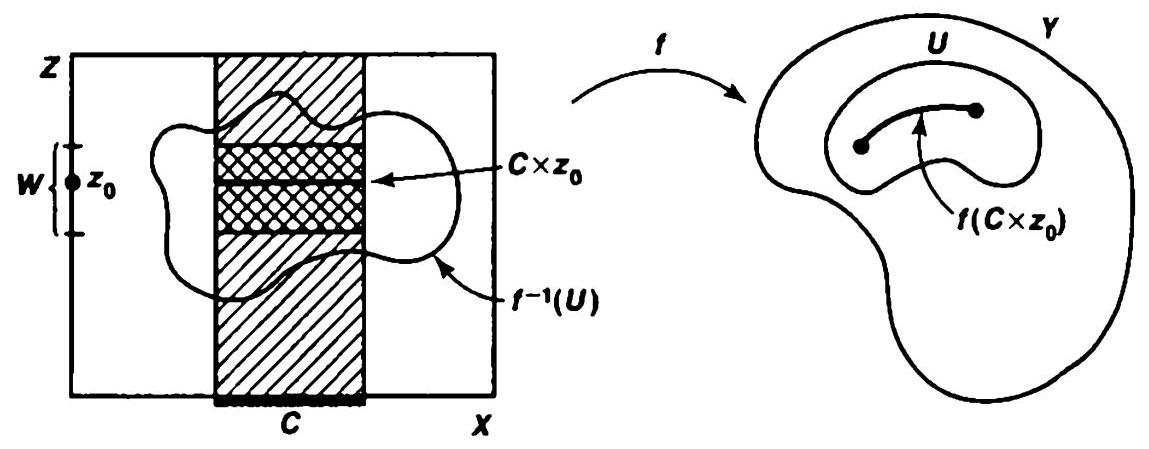
\includegraphics[width=1.0\textwidth]{images/46.2.jpg}
\end{center}
\hspace*{3em} 

Figure 46.2

We discuss briefly the connections between the compact-open topology and the concept of homotopy, which arises in algebraic topology

If \(f\) and \(g\) are continuous maps of \(X\) into \(Y\) , we say that \(f\) and \(g\) are homotopic if there is a continuous map

\[
{hX} \times  \left\lbrack  {0,1}\right\rbrack   \rightarrow  Y
\]

such that \(h\left( {x,0}\right)  = f\left( x\right)\) and \(h\left( {x,1}\right)  = g\left( x\right)\) for each \(x \in  X\) . The map \(h\) is called a homotopy between \(f\) and \(g\) .

Roughly speaking, a homotopy is a "continuous one-parameter family" of maps from \(X\) to \(Y\) More precisely, we note that a homotopy \(h\) gives rise to a map

\[
H.\left\lbrack  {0,1}\right\rbrack   \rightarrow  \mathcal{C}\left( {X,Y}\right)
\]

that assigns, to each parameter value \(t\) in \(\left\lbrack  {0,1}\right\rbrack\) , the corresponding continuous map from \(X\) to \(Y\) . Assuming that \(X\) is locally compact Hausdorff, we see that \(h\) is continuous if and only if \(H\) is continuous This means that a homotopy \(h\) between \(f\) and \(g\) corresponds precisely to a path in the function space \(\mathcal{C}\left( {X,Y}\right)\) from the point \(f\) of \(\mathcal{C}\left( {X,Y}\right)\) to the point \(g\)

We shall return to a more detailed study of homotopy in Part II of the book.
\end{proof}
\section*{Exercises}

1. Show that the sets \({B}_{C}\left( {f,\epsilon }\right)\) form a basis for a topology on \({Y}^{X}\) .

2. Prove Theorem 46.7.

3. Show that the set \(\mathcal{B}\left( {\mathbb{R},\mathbb{R}}\right)\) of bounded functions \(f : \mathbb{R} \rightarrow  \mathbb{R}\) is closed in \({\mathbb{R}}^{\mathbb{R}}\) in the uniform topology, but not in the topology of compact convergence.

4. Consider the sequence of continuous functions \({f}_{n} : \mathbb{R} \rightarrow  \mathbb{R}\) defined by

\[
{f}_{n}\left( x\right)  = x/n
\]

In which of the three topologies of Theorem 46.7 does this sequence converge? Answer the same question for the sequence given in Exercise 9 of §21.

5. Consider the sequence of functions \({f}_{n} : \left( {-1,1}\right)  \rightarrow  \mathbb{R}\) , defined by

\[
{f}_{n}\left( x\right)  = \mathop{\sum }\limits_{{k = 1}}^{n}k{x}^{k}
\]

(a) Show that \(\left( {f}_{n}\right)\) converges in the topology of compact convergence; conclude that the lumit function is continuous. (This is a standard fact about power senes.)

(b) Show that \(\left( {f}_{n}\right)\) does not converge in the uniform topology

6. Show that in the compact-open topology, \(\mathcal{C}\left( {X,Y}\right)\) is Hausdorff if \(Y\) is Hausdorff, and regular if \(Y\) is regular. [Hint: If \(\bar{U} \subset  V\) , then \(\overline{S\left( {C,U}\right) } \subset  S\left( {C,V}\right)\) .

7. Show that if \(Y\) is locally compact Hausdorff, then composition of maps

\[
\mathcal{C}\left( {X,Y}\right)  \times  \mathcal{C}\left( {Y,Z}\right)  \rightarrow  \mathcal{C}\left( {X,Z}\right)
\]

is continuous, provided the compact-open topology is used throughout. [Hint: If \(g \circ  f \in  S\left( {C,U}\right)\) , find \(V\) such that \(f\left( C\right)  \subset  V\) and \(g\left( \bar{V}\right)  \subset  U\) .\}

8. Let \({\mathcal{C}}^{\prime }\left( {X,Y}\right)\) denote the set \(\mathcal{C}\left( {X,Y}\right)\) in some topology \(\mathcal{T}\) . Show that if the evaluation map

\[
e : X \times  {\mathcal{C}}^{\prime }\left( {X,Y}\right)  \rightarrow  Y
\]

is continuous, then \(\mathcal{T}\) contains the compact-open topology. [Hint: The induced map \(E : {\mathcal{C}}^{\prime }\left( {X,Y}\right)  \rightarrow  \mathcal{C}\left( {X,Y}\right)\) is continuous. \(\}\)

9. Here is an (unexpected) application of Theorem 4611 to quotient maps. (Compare Exercise 11 of §29.)

\begin{theorem} If \(p : A \rightarrow  B\) is a quotient map and \(X\) is locally compact Hausdorff, then \({i}_{X} \times  p \cdot  X \times  A \rightarrow  X \times  B\) is a quotient map.
\end{theorem}

Proof.

(a) Let \(Y\) be the quotient space induced by \({i\chi } \times  p\) ; let \(q : X \times  A \rightarrow  Y\) be the quotient map. Show there is a bijective continuous map \(f : Y \rightarrow  X \times  B\) such that \(f \circ  q = {i}_{\chi } \times  p\) .

(b) Let \(g = {f}^{-1}\) . Let \(G : B \rightarrow  \mathcal{C}\left( {X,Y}\right)\) and \(Q : A \rightarrow  \mathcal{C}\left( {X,Y}\right)\) be the maps induced by \(g\) and \(q\) , respectively. Show that \(Q = G \circ  p\) .

(c) Show that \(Q\) is continuous; conclude that \(G\) is continuous, so that \(g\) is continuous.

*10. A space is locally compact if it can be covered by open sets each of which is contained in a compact subspace of \(X\) It is said to be \idxmath{sigma}{\(\sigma\)-compact} \(\sigma\) -compact if it can be covered by countably many such open sets.

(a) Show that if \(X\) is locally compact and second-countable, it is \(\sigma\) -compact.

(b) Let(Y, d)be a metric space. Show that if \(X\) is \(\sigma\) -compact, there is a met-nc for the topology of compact convergence on \({Y}^{X}\) such that if(Y, d)is complete, \({Y}^{X}\) is complete in this metric. [Hint: Let \({A}_{1},{A}_{2},.\) be a countable collection of compact subspaces of \(X\) whose interiors cover \(X\) . Let \({Y}_{t}\) denote the set of all functions from \({A}_{i}\) to \(Y\) , in the uniform topology. Define a homeomorphism of \({Y}^{X}\) with a closed subspace of the product space \({Y}_{1} \times  {Y}_{2} \times  \cdots \}\)

11. Let(Y, d)be a metric space; let \(X\) be a space. Define a topology on \(\mathcal{C}\left( {X,Y}\right)\) as follows: Given \(f \in  \mathcal{C}\left( {X,Y}\right)\) , and given a positive continuous function \(\delta  : X \rightarrow\)  \({\mathbb{R}}_{ + }\) on \(X\) , let

\[
B\left( {f,\delta }\right)  = \{ g \mid  d\left( {f\left( x\right) ,g\left( x\right) }\right)  < \delta \left( x\right) \text{ for all }x \in  X\} .
\]

(a) Show that the sets \(B\left( {f,\delta }\right)\) form a basis for a topology on \(\mathcal{C}\left( {X,Y}\right)\) . We call it the \idx{fine topology}.

(b) Show that the fine topology contains the uniform topology.

(c) Show that if \(X\) is compact, the fine and uniform topologies agree.

(d) Show that if \(X\) is discrete, then \(\mathcal{C}\left( {X,Y}\right)  = {Y}^{X}\) and the fine and box topologies agree.

\section*{§ 47 Ascoli’s Theorem}

Now we prove a more general version of Ascoli's theorem. It characterizes the compact subspaces of \(\mathcal{C}\left( {X,Y}\right)\) in the topology of compact convergence. The proof, however, involves all three of our standard function space topologies: the topology of pointwise convergence, the topology of compact convergence, and the uniform topology.

\begin{theorem}[Ascoli’s theorem] Let \(X\) be a space and let(Y, d)be a metric space. Give \(\mathcal{C}\left( {X,Y}\right)\) the topology of compact convergence; let \(\mathcal{F}\) be a subset of \(\mathcal{C}\left( {X,Y}\right)\) .

(a) If \(\mathcal{F}\) is equicontinuous under \(d\) and the set

\[
{\mathcal{F}}_{a} = \{ f\left( a\right)  \mid  f \in  \mathcal{F}\}
\]

has compact closure for each \(a \in  X\) , then \(\mathcal{F}\) is contained in a compact subspace of \(C\left( {X,Y}\right)\) .

(b) The converse holds if \(X\) is locally compact Hausdorff.
\end{theorem}

Proof of (a). Throughout, we give \({Y}^{X}\) the product topology, which is the same as the topology of pointwise convergence. Then \({Y}^{X}\) is a Hausdorff space. The space \(\mathcal{C}\left( {X,Y}\right)\) , which has the topology of compact convergence, is not a subspace of \({Y}^{X}\) . Let \(\mathcal{G}\) be the closure of \(\mathcal{F}\) in \({Y}^{X}\) .

Step 1. We show that \(\mathcal{G}\) is a compact subspace of \({Y}^{X}\) . Given \(a \in  X\) , let \({C}_{a}\) denote the closure of \({\mathcal{F}}_{a}\) in \(Y\) ; by hypothesis, \({C}_{a}\) is a compact subspace of \(Y\) . The set \(\mathcal{F}\) is contained in the product space

\[
\mathop{\prod }\limits_{{a \in  X}}{C}_{a}
\]

since this product by definition consists of all functions \(f : X \rightarrow  Y\) satisfying the condition \(f\left( a\right)  \in  {C}_{a}\) for all \(a\) . This product space is compact, by the Tychonoff theorem; it is a closed subspace of the product space \({Y}^{X}\) . Because \(\mathcal{G}\) equals the closure of \(\mathcal{F}\) in \({Y}^{X},\mathcal{G}\) is contained in \(\prod {C}_{a}\) , being closed, \(\mathcal{G}\) is therefore compact.

Step 2. We show that each function belonging to \(\mathcal{G}\) is continuous, and indeed that \(\mathcal{G}\) itself is equicontinuous under \(d\) .

Given \({x}_{0} \in  X\) and \(\epsilon  > 0\) , choose a neighborhood \(U\) of \({x}_{0}\) such that

(*)
\[
d\left( {f\left( x\right) ,f\left( {x}_{0}\right) }\right)  < \epsilon /3\;\text{ for all }f \in  \mathcal{F}\text{ and all }x \in  U.
\]

We shall show that \(d\left( {g\left( x\right) ,g\left( {x}_{0}\right) }\right)  < \epsilon\) for all \(g \in  \mathcal{G}\) and all \(x \in  U\) ; it follows that \(\mathcal{G}\) is equicontinuous.

Let \(g \in  \mathcal{G}\) and let \(x\) be a point of \(U\) Define \({V}_{x}\) to be the subset of \({Y}^{X}\) , open in \({Y}^{X}\) , consisting of all elements \(h\) of \({Y}^{X}\) such that

\[
\left( {* * }\right)
\]

\[
d\left( {h\left( x\right) ,g\left( x\right) }\right)  < \epsilon /3\;\text{ and }\;d\left( {h\left( {x}_{0}\right) ,g\left( {x}_{0}\right) }\right)  < \epsilon /3.
\]

Because \(g\) belongs to the closure of \(\mathcal{F}\) , the neighborhood \({V}_{x}\) of \(g\) must contain an element \(f\) of \(\mathcal{F}\) . Applying the triangle inequality to \(\left( *\right)\) and \(\left( {* * }\right)\) , it follows that \(d\left( {g\left( x\right) ,g\left( {x}_{0}\right) }\right)  < \epsilon\) , as desired.

Step 3. We show that the product topology on \({Y}^{X}\) and the compact convergence topology on \(\mathcal{C}\left( {X,Y}\right)\) coincide on the subset \(\mathcal{G}\) .

In general, the compact convergence topology is finer than the product topology. We prove that the reverse holds for the subset \(\mathcal{G}\) . Let \(g\) be an element of \(\mathcal{G}\) , and let \({B}_{C}\left( {g,\epsilon }\right)\) be a basis element for the compact convergence topology on \({Y}^{X}\) that contains \(g\) . We find a basis element \(B\) for the pointwise convergence topology on \({Y}^{X}\) that contains \(g\) such that

\[
\left\lbrack  {B \cap  \mathcal{G}}\right\rbrack   \subset  \left\lbrack  {{B}_{C}\left( {g,\epsilon }\right)  \cap  \mathcal{G}}\right\rbrack  .
\]

Using equicontinuity of \(\mathcal{G}\) and compactness of \(C\) , we can cover \(C\) by finitely many open sets \({U}_{1},\ldots ,{U}_{n}\) of \(X\) , containing points \({x}_{1},\ldots ,{x}_{n}\) , respectively, such that for each \(i\) , we have

\[
d\left( {g\left( x\right) ,g\left( {x}_{i}\right) }\right)  < \epsilon /3
\]

for \(x \in  {U}_{i}\) and \(g \in  \mathcal{G}\) . Then we define \(B\) to be the basis element for \({Y}^{X}\) defined by the equation

\[
B = \left\{  {h \mid  h \in  {Y}^{X}}\right. \text{ and }d\left( {h\left( {x}_{i}\right) ,g\left( {x}_{i}\right) }\right)  < \epsilon /3\text{ for }\left. {i = 1,\ldots ,n}\right\}  \text{ . }
\]

We show that if \(h\) is an element of \(B \cap  \mathcal{G}\) , then \(h\) belongs to \({B}_{C}\left( {g,\epsilon }\right)\) . That is, we show that \(d\left( {h\left( x\right) ,g\left( x\right) }\right)  < \epsilon\) for \(x \in  C\) . Given \(x \in  C\) , choose \(i\) so that \(x \in  {U}_{i}\) . Then

\[
d\left( {h\left( x\right) ,h\left( {x}_{i}\right) }\right)  < \epsilon /3\;\text{ and }
\]

\[
d\left( {g\left( x\right) ,g\left( {x}_{i}\right) }\right)  < \epsilon /3
\]

because \(x \in  {U}_{i}\) and \(g,h \in  \mathcal{g}\) , while

\[
d\left( {h\left( {x}_{i}\right) ,g\left( {x}_{i}\right) }\right)  < \epsilon /3
\]

because \(h \in  B\) . It follows from the triangle inequality that \(d\left( {h\left( x\right) ,g\left( x\right) }\right)  < \epsilon\) , as desired.

Step 4. We complete the proof. The set \(\mathcal{G}\) contains \(\mathcal{F}\) and is contained in \(\mathcal{C}\left( {X,Y}\right)\) . It is compact as a subspace of \({Y}^{X}\) in the product topology. By the result just proved, it is also compact as a subspace of \(\mathcal{C}\left( {X,Y}\right)\) in the compact convergence topology.

Proof of (b). Let \(\mathcal{H}\) be a compact subspace of \(\mathcal{C}\left( {X,Y}\right)\) that contains \(\mathcal{F}\) . We show that \(\mathcal{H}\) is equicontinuous and that \({\mathcal{H}}_{a}\) is compact for each \(a \in  X\) . It follows that \(\mathcal{F}\) is equicontinuous (since \(\mathcal{F} \subset  \mathcal{H}\) ), and that \({\mathcal{F}}_{a}\) lies in the compact subspace \({\mathcal{H}}_{a}\) of \(Y\) , so that \({\widetilde{\mathcal{F}}}_{a}\) is compact.

To show \({\mathcal{H}}_{a}\) is compact, consider the composite of the map

\[
j : \mathcal{C}\left( {X,Y}\right)  \rightarrow  X \times  \mathcal{C}\left( {X,Y}\right)
\]

defined by \(j\left( f\right)  = a \times  f\) , and the evaluation map

\[
e : X \times  \mathcal{C}\left( {X,Y}\right)  \rightarrow  Y
\]

given by the equation \(e\left( {x \times  f}\right)  = f\left( x\right)\) . The map \(j\) is obviously continuous, and the map \(e\) is continuous by Theorems 46.8 and 46.10. The composite \(e \circ  j\) maps \(\mathcal{H}\) to \({\mathcal{H}}_{a}\) ; since \(\mathcal{H}\) is compact, so is \({\mathcal{H}}_{a}\) .

Now we show that \(\mathcal{H}\) is equicontinuous at \(a\) , relative to the metric \(d\) . Let \(A\) be a compact subspace of \(X\) that contains a neighborhood of \(a\) . It suffices to show that the subset

\[
\mathcal{R} = \{ f \mid  A;f \in  \mathcal{H}\}
\]

of \(\mathcal{C}\left( {A,Y}\right)\) is equicontinuous at \(a\) .

Give \(\mathcal{C}\left( {A,Y}\right)\) the compact convergence topology. We show that the restriction map

\[
r : \mathcal{C}\left( {X,Y}\right)  \rightarrow  \mathcal{C}\left( {A,Y}\right)
\]

is continuous. Let \(f\) be an element of \(\mathcal{C}\left( {X,Y}\right)\) and let \(B = {B}_{C}\left( {f \mid  A,\epsilon }\right)\) be a basis element for \(\mathcal{C}\left( {A,Y}\right)\) containing \(f \mid  A\) , where \(C\) is a compact subspace of \(A\) . Then \(C\) is a compact subspace of \(X\) , and \(r\) maps the neighborhood \({B}_{C}\left( {f,\epsilon }\right)\) of \(f\) in \(\mathcal{C}\left( {X,Y}\right)\) into \(B\) .

The map \(r\) maps \(\mathcal{H}\) onto \(\mathcal{R}\) ; because \(\mathcal{H}\) is compact, so is \(\mathcal{R}\) . Now \(\mathcal{R}\) is a subspace of \(\mathcal{C}\left( {A,Y}\right)\) ; because \(A\) is compact, the compact convergence and the uniform topologies on \(\mathcal{C}\left( {A,Y}\right)\) coincide. It follows from Theorem 45.1 that \(\mathcal{R}\) is totally bounded in the uniform metric on \(\mathcal{C}\left( {A,Y}\right)\) ; then Lemma 45.2 implies that \(\mathcal{R}\) is equicontinuous relative to \(d\) .

An even more general version of Ascoli's theorem may be found in 		\cite{Kelley1991} or 		\cite{Willard1970}. There it is not assumed that \(Y\) is a metric space, but only that it has what is called a uniform structure, which is a generalization of the notion of metric.

Ascoli's theorem has many applications in analysis, but these lie outside the scope of this book. See 		\cite{KolmogorovFomin1957} for several such applications.

\section*{Exercises}

1. Which of the following subsets of \(\mathcal{C}\left( {\mathbb{R},\mathbb{R}}\right)\) are pointwise bounded? Which are equicontinuous?

(a) The collection \(\left\{  {f}_{n}\right\}\) , where \({f}_{n}\left( x\right)  = x + \sin {nx}\) .

(b) The collection \(\left\{  {g}_{n}\right\}\) , where \({g}_{n}\left( x\right)  = n + \sin x\) .

(c) The collection \(\left\{  {h}_{n}\right\}\) , where \({h}_{n}\left( x\right)  = {\left| x\right| }^{1/n}\) .

(d) The collection \(\left\{  {k}_{n}\right\}\) , where \({k}_{n}\left( x\right)  = n\sin \left( {x/n}\right)\) .

2. Prove the following

\begin{theorem} If \(X\) is a locally compact Hausdorff space, then a subspace \(\mathcal{F}\) of \(\mathcal{C}\left( {X,{\mathbb{R}}^{n}}\right)\) in the topology of compact convergence has compact closure if and only if \(\mathcal{F}\) is pointwise bounded and equicontinuous under either of the standard metrics on \({\mathbb{R}}^{n}\) .
\end{theorem}

3. Show that the general version of Ascoli’s theorem implies the classical version (Theorem 45.4) when \(X\) is Hausdorff.

4. Prove the following:

\begin{theorem}[Arzela’s theorem, general version] Let \(X\) be a Hausdorff space that is \(\sigma\) -compact; let \({f}_{n}\) be a sequence of functions \({f}_{n} : X \rightarrow  {\mathbb{R}}^{k}\) . If the collection \(\left\{  {f}_{n}\right\}\) is pointwise bounded and equicontinuous, then the sequence \({f}_{n}\) has a subsequence that converges, in the topology of compact convergence, to a continuous function.
\end{theorem}

\{Hint: Show \(\mathcal{C}\left( {X,{\mathbb{R}}^{k}}\right)\) is first-countable.\}

5. Let(Y, d)be a metric space; let \({f}_{n} : X \rightarrow  Y\) be a sequence of continuous functions; let \(f : X \rightarrow  Y\) be a function (not necessarily continuous). Suppose \({f}_{n}\) converges to \(f\) in the topology of pointwise convergence. Show that if \(\left\{  {f}_{n}\right\}\) is equicontinuous, then \(f\) is continuous and \({f}_{n}\) converges to \(f\) in the topology of compact convergence.

\chapter{Baire Spaces and Dimension Theory}

In this chapter, we introduce a class of topological spaces called the \idx{Baire space}s. The defining condition for a Baire space is a bit complicated to state, but it is often useful in the applications, in both analysis and topology. Most of the spaces we have been studying are Baire spaces. For instance, a Hausdorff space is a Baire space if it is \idx{Compact Hausdorff space: is Baire space} compact, or even \idx{Locally compact Hausdorff space: Baire condition} locally compact. And a metrizable space \(X\) is a Baire space if It is topologically complete, that is, if there is a metric for \(X\) relative to which \(X\) is complete.

It follows that, since the space \(\mathcal{C}\left( {X,{\mathbb{R}}^{n}}\right)\) of all continuous functions from a space \(X\) to \({\mathbb{R}}^{n}\) is complete in the \idx{Uniform structure} uniform metric, it is a Baire space in the uniform topology. This fact has a number of interesting applications.

One application is the proof we give in \(\$ {49}\) of the existence of a continuous nowhere-differentiable real-valued function.

Another application arises in that branch of topology called \idx{Dimension, topological} dimension theory. In \(\$ {50}\) , we define a topological notion of dimension, due to Lebesgue. And we prove the classical theorem that every compact metrizable space of \idx{topological dimension} \(m\) can be imbedded in euclidean space \({\mathbb{R}}^{N}\) of dimension \(N = {2m} + 1\) . It follows that every compact \(m\) -manifold can be imbedded in \({\mathbb{R}}^{{2m} + 1}\) This generalizes the imbedding theorem proved in §36.

Throughout the chapter, we assume familiarity with complete metric spaces (§43). When we study dimension theory, we shall make use of §36, Imbeddings of Manifolds, as well as a bit of linear algebra.

\section*{§ 48 Baire Spaces}

The defining condition for a Baire space is probably as "unnatural looking" as any condition we have yet introduced in this book. But bear with us awhile.

In this section, we shall define Baure spaces and shall show that two important classes of spaces-the complete metric spaces and the compact Hausdorff spaces-are contained in the class of Baire spaces. Then we shall give some applications, which, even if they do not make the Baire condition seem any more natural, will at least show what a useful tool it can be. In fact, it turns out to be a very useful and fairly sophisticated tool in both analysis and topology.

\begin{definition} Recall that if \(A\) is a subset of a space \(X\) , the interior of \(A\) is defined as the union of all open sets of \(X\) that are contained in \(A\) . To say that \(A\) has \idx{empty interior} is to say then that \(A\) contains no open set of \(X\) other than the empty set. Equivalently, \(A\) has empty interior if every point of \(A\) is a limit point of the complement of \(A\) , that is, if the complement of \(A\) is dense in \(X\) .
\end{definition}

\begin{example} The set \(\mathbb{Q}\) of rationals has emply interior as a subset of \(\mathbb{R}\) , but the interval \(\left\lbrack  {0,1}\right\rbrack\) has nonempty interior The interval \(\left\lbrack  {0,1}\right\rbrack   \times  0\) has empty interior as a subset of the plane \({\mathbb{R}}^{2}\) , and so does the subset \(\mathbb{Q} \times  \mathbb{R}\) .
\end{example}

\begin{definition} A space \(X\) is said to be a Baire space if the following condition holds: Given any countable collection \(\left\{  {A}_{n}\right\}\) of closed sets of \(X\) each of which has empty interior in \(X\) , their union \(\bigcup {A}_{n}\) also has empty interior in \(X\) .
\end{definition}

\begin{example} The space \(\mathbb{Q}\) of rationals is not a Baire space. For each one-point set in \(\mathbb{Q}\) is closed and has empty interior in \(\mathbb{Q}\) , and \(\mathbb{Q}\) is the countable union of its one-point subsets.
\end{example}

The space \({\mathbb{Z}}_{ + }\) , on the other hand, does form a Baire space Every subset of \({\mathbb{Z}}_{ + }\) is open, so that there exist no subsets of \({\mathbb{Z}}_{ + }\) having empty interior, except for the empty set. Therefore, \({\mathbb{Z}}_{ + }\) satisfies the Baire condition vacuously.

More generally, every closed subspace of \(\mathbb{R}\) , being a complete metric space, is a Baire space. Somewhat surprising is the fact that the irrationals in \(\mathbb{R}\) also form a Baire space; see Exercise 6

The terminology originally used by R. Baire for this concept involved the word "category." A subset \(A\) of a space \(X\) was said to be of the \idx{First category set} first category in \(X\) if it was contained in the union of a countable collection of closed sets of \(X\) having empty interiors in \(X\) ; otherwise, it was said to be of the \idx{Second category set} second category in \(X\) . Using this terminology, we can say the following:

A space \(X\) is a Baire space if and only if every nonempty open set in \(X\) is ofthe second category

We shall not use the terms "first category" and "second category" in this book.

The preceding definition is the "closed set definition" of a Baire space. There is also a formulation involving open sets that is frequently useful. It is given in the following lemma.

\begin{lemma} \(X\) is a Baire space if and only if given any countable collection \(\left\{  {U}_{n}\right\}\) of open sets in \(X\) , each of which is dense in \(X\) , their intersection \(\cap  {U}_{n}\) is also dense in \(X\) .
\end{lemma}

\begin{proof}Recall that a set \(C\) is dense in \(X\) if \(\bar{C} = X\) . The theorem now follows at once from the two remarks:
(1) \(A\) is closed in \(X\) if and only if \(X - A\) is open in \(X\) .

(2) \(B\) has empty interior in \(X\) if and only if \(X - B\) is dense in \(X\) .

There are a number of theorems giving conditions under which a space is a Baire space. The most important is the following:
\end{proof}
\begin{theorem}[\idx{Baire category theorem}] If \(X\) is a compact Hausdorff space or a complete metric space, then \(X\) is a Baire space.
\end{theorem}

\begin{proof}Given a countable collection \(\left\{  {A}_{n}\right\}\) of closed set of \(X\) having empty interiors, we want to show that their union \(\bigcup {A}_{n}\) also has empty interior in \(X\) . So, given the nonempty open set \({U}_{0}\) of \(X\) , we must find a point \(x\) of \({U}_{0}\) that does not lie in any of the sets \({A}_{n}\) .
Consider the first set \({A}_{1}\) . By hypothesis, \({A}_{1}\) does not contain \({U}_{0}\) . Therefore, we may choose a point \(y\) of \({U}_{0}\) that is not in \({A}_{1}\) . Regularity of \(X\) , along with the fact that \({A}_{1}\) is closed, enables us to choose a neighborhood \({U}_{1}\) of \(y\) such that

\[
{\bar{U}}_{1} \cap  {A}_{1} = \varnothing
\]

\[
{\bar{U}}_{1} \subset  {U}_{0}\text{ . }
\]

If \(X\) is metric, we also choose \({U}_{1}\) small enough that its diameter is less than1.

In general, given the nonempty open set \({U}_{n - 1}\) , we choose a point of \({U}_{n - 1}\) that is not in the closed set \({A}_{n}\) , and then we choose \({U}_{n}\) to be a neighborhood of this point such that

\[
{\bar{U}}_{n} \cap  {A}_{n} = \varnothing
\]

\[
{\bar{U}}_{n} \subset  {U}_{n - 1},
\]

\[
\text{ diam }{U}_{n} < 1/n\text{ in the metric case. }
\]

We assert that the intersection \(\cap  {\bar{U}}_{n}\) is nonempty. From this fact, our theorem will follow. For if \(x\) is a point of \(\bigcap {\bar{U}}_{n}\) , then \(x\) is in \({U}_{0}\) because \({\bar{U}}_{1} \subset  {U}_{0}\) . And for each \(n\) , the point \(x\) is not in \({A}_{n}\) because \({\bar{U}}_{n}\) is disjoint from \({A}_{n}\) .

The proof that \(\cap  {\widetilde{U}}_{n}\) is nonempty splits into two parts, depending on whether \(X\) is compact Hausdorff or complete metric. If \(X\) is compact Hausdorff, we consider the nested sequence \({\bar{U}}_{1} \supset  {\bar{U}}_{2} \supset  \cdots\) of nonempty subsets of \(X\) . The collection \(\left\{  {\bar{U}}_{n}\right\}\) has the finite intersection property; since \(X\) is compact, the intersection \(\cap  {U}_{n}\) must be nonempty.

If \(X\) is complete metric, we apply the following lemma.
\end{proof}
\begin{lemma} Let \({C}_{1} \supset  {C}_{2} \supset   \cdot   \cdot\) be a nested sequence of nonempty closed sets in the complete metric space \(X\) . If \(\operatorname{diam}{C}_{n} \rightarrow  0\) , then \(\cap  {C}_{n} \neq  \varnothing\) .
\end{lemma}

\begin{proof}We gave this as an exercise in \(§{43}\) . Here is a proof: Choose \({x}_{n} \in  {C}_{n}\) for each \(n\) . Because \({x}_{n},{x}_{m} \in  {C}_{N}\) for \(n,m \geq  N\) , and because \(\operatorname{diam}{C}_{N}\) can be made less than any given \(\epsilon\) by choosing \(N\) large enough, the sequence \(\left( {x}_{n}\right)\) is a Cauchy sequence. Suppose that it converges to \(x\) . Then for given \(k\) , the subsequence \({x}_{k},{x}_{k + 1},\ldots\) also converges to \(x\) . Thus \(x\) necessarily belongs to \({\widetilde{C}}_{k} = {C}_{k}\) . Then \(x \in  \bigcap {C}_{k}\) , as desired.
Here is one application of the theory of Baire spaces; we shall give further applications in the sections that follow. This application is perhaps more amusing than profound. It concerns a question that a student might ask concerning convergent sequences of continuous functions.

Let \({f}_{n} : \left\lbrack  {0,1}\right\rbrack   \rightarrow  \mathbb{R}\) be a sequence of continuous functions such that \({f}_{n}\left( x\right)  \rightarrow\)  \(f\left( x\right)\) for each \(x \in  \left\lbrack  {0,1}\right\rbrack\) . There are examples that show the limit function \(f\) need not be continuous. But one might wonder just how discontinuous \(f\) can be Could it be discontinuous everywhere, for instance? The answer is "no." We shall show that \(f\) must be continuous at infinitely many \idx{End points of arc} points of \(\left\lbrack  {0,1}\right\rbrack\) . In fact, the set of points at which \(f\) is continuous is dense in \(\left\lbrack  {0,1}\right\rbrack\) !

To prove this result, we need the following lemma:

*Lemma 48.4. Any open subspace \(Y\) of a Baire space \(X\) is itself a Baire space.

Proof. Let \({A}_{n}\) be a countable collection of closed sets of \(Y\) that have empty interiors in \(Y\) . We show that \(\bigcup {A}_{n}\) has empty interior in \(Y\) .

Let \({\bar{A}}_{n}\) be the closure of \({A}_{n}\) in \(X\) ; then \({\bar{A}}_{n} \cap  Y = {A}_{n}\) . The set \({\bar{A}}_{n}\) has empty interior in \(X\) . For if \(U\) is a nonempty open set of \(X\) contained in \({\bar{A}}_{n}\) , then \(U\) must intersect \({A}_{n}\) . Then \(U \cap  Y\) is a nonempty open set of \(Y\) contained in \({A}_{n}\) , contrary to hypothesis

If the union of the sets \({A}_{n}\) contains the nonempty open set \(W\) of \(Y\) , then the union of the sets \({A}_{n}\) also contains the set \(W\) , which is open in \(X\) because \(Y\) is open in \(X\) . But each set \({\bar{A}}_{n}\) has empty interior in \(X\) , contradicting the fact that \(X\) is a Baire space.

*Theorem 48.5. Let \(X\) be a space; let(Y, d)be a metric space. Let \({f}_{n} : X \rightarrow  Y\) be a sequence of continuous functions such that \({f}_{n}\left( x\right)  \rightarrow  f\left( x\right)\) for all \(x \in  X\) , where \(f : X \rightarrow  Y\) . If \(X\) is a Baire space, the set of points at which \(f\) is continuous is dense in \(X\) .

Proof. Given a positive integer \(N\) and given \(\epsilon  > 0\) , define

\[
{A}_{N}\left( \epsilon \right)  = \left\lbrack  {x \mid  d\left( {{f}_{n}\left( x\right) ,{f}_{m}\left( x\right) }\right)  \leq  \epsilon }\right. \text{ for all }\left. {n,m \geq  N}\right\}  \text{ . }
\]

Note that \({A}_{N}\left( \epsilon \right)\) is closed in \(X\) . For the set of those \(x\) for which \(d\left( {{f}_{n}\left( x\right) ,{f}_{m}\left( x\right) }\right)  \leq  \epsilon\) is closed in \(X\) , by continuity of \({f}_{n}\) and \({f}_{m}\) , and \({A}_{N}\left( \epsilon \right)\) is the intersection of these sets for all \(n,m \geq  N\) .

For fixed \(\epsilon\) , consider the sets \({A}_{1}\left( \epsilon \right)  \subset  {A}_{2}\left( \epsilon \right)  \subset  \cdots\) . The union of these sets is all of \(X\) . For, given \({x}_{0} \in  X\) , the fact that \({f}_{n}\left( {x}_{0}\right)  \rightarrow  f\left( {x}_{0}\right)\) implies that the sequence \({f}_{n}\left( {x}_{0}\right)\) is a Cauchy sequence; hence \({x}_{0} \in  {A}_{N}\left( \epsilon \right)\) for some \(N\) .

Now let

\[
U\left( \epsilon \right)  = \mathop{\bigcup }\limits_{{N \in  {\mathbf{Z}}_{ + }}}\operatorname{Int}{A}_{N}\left( \epsilon \right)
\]

We shall prove two things:

(1) \(U\left( \epsilon \right)\) is open and dense in \(X\) .

(2) The function \(f\) is continuous at each point of the set

\[
C = U\left( 1\right)  \cap  U\left( {1/2}\right)  \cap  U\left( {1/3}\right)  \cap  \cdots .
\]

Our theorem then follows from the fact that \(X\) is a Baire space.

To show that \(U\left( \epsilon \right)\) is dense in \(X\) , it suffices to show that for any nonempty open set \(V\) of \(X\) , there is an \(N\) such that the set \(V \cap  \operatorname{Int}{A}_{N}\left( \epsilon \right)\) is nonempty. For this purpose, we note first that for each \(N\) , the set \(V \cap  {A}_{N}\left( \epsilon \right)\) is closed in \(V\) . Because \(V\) is a Baire space by the preceding lemma, at least one of these sets, say \(V \cap  {A}_{M}\left( \epsilon \right)\) , must contain a nonempty open set \(W\) of \(V\) Because \(V\) is open in \(X\) , the set \(W\) is open in \(X\) ; therefore, it is contained in Int \({A}_{M}\left( \epsilon \right)\) .

Now we show that if \({x}_{0} \in  C\) , then \(f\) is continuous at \({x}_{0}\) . Given \(\epsilon  > 0\) , we shall find a neighborhood \(W\) of \({x}_{0}\) such that \(d\left( {f\left( x\right) ,f\left( {x}_{0}\right) }\right)  < \epsilon\) for \(x \in  W\) .

First, choose \(k\) so that \(1/k < \epsilon /3\) . Since \({x}_{0} \in  C\) , we have \({x}_{0} \in  U\left( {1/k}\right)\) ; therefore, there is an \(N\) such that \({x}_{0} \in  \operatorname{Int}{A}_{N}\left( {1/k}\right)\) . Finally, continuity of the function \({f}_{N}\) enables us to choose a neighborhood \(W\) of \({x}_{0}\) , contained in \({A}_{N}\left( {1/k}\right)\) , such that

(*)
\[
d\left( {{f}_{N}\left( x\right) ,{f}_{N}\left( {x}_{0}\right) }\right)  < \epsilon /3\;\text{ for }x \in  W.
\]

The fact that \(W \subset  {A}_{N}\left( {1/k}\right)\) implies that

\[
d\left( {{f}_{n}\left( x\right) ,{f}_{N}\left( x\right) }\right)  \leq  1/k\;\text{ for }n \geq  N\text{ and }x \in  W.
\]

Letting \(n \rightarrow  \infty\) , we obtain the inequality

\[
\left( {* * }\right)
\]

\[
d\left( {f\left( x\right) ,{f}_{N}\left( x\right) }\right)  \leq  1/k < \epsilon /3\;\text{ for }x \in  W.
\]

In particular, since \({x}_{0} \in  W\) , we have

\[
\left( {* *  * }\right)
\]

\[
d\left( {f\left( {x}_{0}\right) ,{f}_{N}\left( {x}_{0}\right) }\right)  < \epsilon /3.
\]

Applying the triangle inequality to \(\left( *\right) ,\left( {* * }\right)\) , and \(\left( {* *  * }\right)\) gives us our desired result.
\end{proof}
\section*{Exercises}

1. Let \(X\) equal the countable union \(\cup  {B}_{n}\) . Show that if \(X\) is a nonempty Baire space, at least one of the sets \({\bar{B}}_{n}\) has a nonempty interior.

2. The Baire category theorem implies that \(\mathbb{R}\) cannot be written as a countable union of closed subsets having empty interiors. Show this fails if the sets are not required to be closed

3. Show that every locally compact Hausdorff space is a Baire space.

4. Show that if every point \(x\) of \(X\) has a neighborhood that is a Barre space, then \(X\) is a Baure space. [Hint: Use the open set formulation of the Baure condition.\}

5. Show that if \(Y\) is a \({G}_{\delta }\) set in \(X\) , and if \(X\) is compact Hausdorff or complete metric, then \(Y\) is a Baire space in the subspace topology. [Hint: Suppose that \(Y = \bigcap {W}_{n}\) , where \({W}_{n}\) is open in \(X\) , and that \({B}_{n}\) is closed in \(Y\) and has empty interior in \(Y\) . Given \({U}_{0}\) open in \(X\) with \({U}_{0} \cap  Y \neq  \varnothing\) , find a sequence of open sets \({U}_{n}\) of \(X\) with \({U}_{n} \cap  Y\) nonempty, such that

\[
{\bar{U}}_{n} \subset  {U}_{n - 1},
\]

\[
{\bar{U}}_{n} \cap  {\bar{B}}_{n} = \varnothing
\]

\[
\operatorname{diam}{U}_{n} < 1/n\;\text{ in the metric case, }
\]

\[
\left. {{\bar{U}}_{n} \subset  {W}_{n}}\right\}
\]

6. Show that the irrationals are a Baire space.

7. Prove the following:

\begin{theorem} If \(D\) is a countable dense subset of \(\mathbb{R}\) , there is no function \(f : \mathbb{R} \rightarrow  \mathbb{R}\) that is continuous precisely at the points of \(D\)
\end{theorem}

Proof.

(a) Show that if \(f : \mathbb{R} \rightarrow  \mathbb{R}\) , then the set \(C\) of points at which \(f\) is continuous is a \({G}_{\delta }\) set in \(\mathbb{R}\) . [Hint: Let \({U}_{n}\) be the union of all open sets \(U\) of \(\mathbb{R}\) such that \(\operatorname{diam}f\left( U\right)  < 1/n\) . Show that \(C = \bigcap {U}_{n}\) .\}

(b) Show that \(D\) is not a \({G}_{\delta }\) set in \(\mathbb{R}\) . [Hint: Suppose \(D = \bigcap {W}_{n}\) , where \({W}_{n}\) is open in \(\mathbb{R}\) . For \(d \in  D\) , set \({V}_{d} = \mathbb{R} - \lbrack d\}\) . Show \({W}_{n}\) and \({V}_{d}\) are dense in \(\mathbb{R}\) .

8. If \({f}_{n}\) is a sequence of continuous functions \({f}_{n} : \mathbb{R} \rightarrow  \mathbb{R}\) such that \({f}_{n}\left( x\right)  \rightarrow  f\left( x\right)\) for each \(x \in  \mathbb{R}\) , show that \(f\) is continuous at uncountably many points of \(\mathbb{R}\) .

9. Let \(g : {\mathbb{Z}}_{ + } \rightarrow  \mathbb{Q}\) be a bijective function; let \({x}_{n} = g\left( n\right)\) . Define \(f : \mathbb{R} \rightarrow  \mathbb{R}\) as follows:

\[
f\left( {x}_{n}\right)  = 1/n\;\text{ for }{x}_{n} \in  \mathbb{Q},
\]

\[
f\left( x\right)  = 0\;\text{ for }x \notin  \mathbb{Q}
\]

Show that \(f\) is continuous at each irrational and discontinuous at each rational. Can you find a sequence of continuous functions \({f}_{n}\) coverging to \(f\) ?

10. Prove the following:

\begin{theorem}[\idx{Uniform boundedness principle}] Let \(X\) be a complete metric space, and let \(\mathcal{F}\) be a subset of \(\mathcal{C}\left( {X,\mathbb{R}}\right)\) such that for each \(a \in  X\) , the set

\[
{\mathcal{F}}_{a} = \{ f\left( a\right)  \mid  f \in  \mathcal{F}\}
\]

is bounded. Then there is a nonempty open set \(U\) of \(X\) on which the functions in \(\mathcal{F}\) are uniformly bounded, that is, there is a number \(M\) such that \(\left| {f\left( x\right) }\right|  \leq  M\) for all \(x \in  U\) and all \(f \in  \mathcal{F}\) . [Hint: Let \({A}_{N} = \{ x;\left| {f\left( x\right) }\right|  \leq  N\) for all \(f \in  \mathcal{F}\}\) .]
\end{theorem}

11. Determine whether or not \({\mathbb{R}}_{\ell }\) is a Baire space

12. Show that \({\mathbb{R}}^{J}\) is a Baire space in the box, product, and uniform topologies.

*13. Let \(X\) be a topological space; let \(Y\) be a complete metric space. Show that \(\mathcal{C}\left( {X,Y}\right)\) is a Baire space in the fine topology (see Exercise 11 of §46). [Hint: Given basis elements \(B\left( {{f}_{i},{\delta }_{i}}\right)\) such that \({\delta }_{1} \leq  1\) and \({\delta }_{i + 1} \leq  {\delta }_{i}/3\) and \({f}_{i + 1} \in\)  \(B\left( {{f}_{i},{\delta }_{i}/3}\right)\) , show that

\[
\bigcap B\left( {{f}_{i},{\delta }_{i}}\right)  \neq  \varnothing \text{ .] }
\]

\section*{*§ 49 A Nowhere-Differentiable Function}

We prove the following result from analysis:

\begin{theorem} Let \(h : \left\lbrack  {0,1}\right\rbrack   \rightarrow  \mathbb{R}\) be a continuous function. Given \(\epsilon  > 0\) , there is a function \(g : \left\lbrack  {0,1}\right\rbrack   \rightarrow  \mathbb{R}\) with \(\left| {h\left( x\right)  - g\left( x\right) }\right|  < \epsilon\) for all \(x\) , such that \(g\) is continuous and nowhere differentiable.
\end{theorem}

\begin{proof}Let \(I = \left\lbrack  {0,1}\right\rbrack\) . Consider the space \(\mathcal{C} = \mathcal{C}\left( {I,\mathbb{R}}\right)\) of continuous maps from \(I\) to \(\mathbb{R}\) , in the metric
\[
\rho \left( {f,g}\right)  = \max \{ \left| {f\left( x\right)  - g\left( x\right) }\right| \} .
\]

This space is a complete metric space and, therefore, is a Bare space. We shall define, for each \(n\) , a certain subset \({U}_{n}\) of \(\mathcal{C}\) that is open in \(\mathcal{C}\) and dense in \(\mathcal{C}\) , and has the property that the functions belonging to the intersection

\[
\mathop{\bigcap }\limits_{{n \in  {\mathbf{Z}}_{ + }}}{U}_{n}
\]

are nowhere differentiable. Because \(\mathcal{C}\) is a Baire space, this intersection is dense in \(\mathcal{C}\) , by Lemma 48.1. Therefore, given \(h\) and \(\epsilon\) , this intersection must contain a function \(g\) such that \(\rho \left( {h,g}\right)  < \epsilon\) . The theorem follows.

The tricky part is to define the set \({U}_{n}\) properly. We first take a function \(f\) and consider its difference quotients. Given \(x \in  I\) and given \(0 < h \leq  \frac{1}{2}\) , consider the expressions

\[
\left| \frac{f\left( {x + h}\right)  - f\left( x\right) }{h}\right| \;\text{ and }\;\left| \frac{f\left( {x - h}\right)  - f\left( x\right) }{-h}\right| .
\]

Since \(h \leq  \frac{1}{2}\) , at least one of the numbers \(x + h\) and \(x - h\) belongs to \(I\) , so that at least one of these expressions is defined. Let \({\Delta f}\left( {x,h}\right)\) denote the larger of the two if both are defined; otherwise, let it denote the one that is defined. If the derivative \({f}^{\prime }\left( x\right)\) of \(f\) at \(x\) exists, it equals the limit of these difference quotients, so that

\[
\left| {{f}^{\prime }\left( x\right) }\right|  = \mathop{\lim }\limits_{{h \rightarrow  0}}{\Delta f}\left( {x,h}\right) .
\]

We seek to find a continuous function for which this limit does not exist. To be specific, we shall construct \(f\) so that given \(x\) , there is a sequence of numbers \({h}_{n}\) converging to 0 for which the numbers \({\Delta f}\left( {x,{h}_{n}}\right)\) become arbitrarily large.

This gives us the idea for defining the set \({U}_{n}\) . Given any positive number \(h \leq  1/2\) , let

\[
{\Delta }_{h}f = \inf \{ {\Delta f}\left( {x,h}\right)  \mid  x \in  I\}
\]

Then for \(n \geq  2\) , we define \({U}_{n}\) by declaring that a function \(f\) belongs to \({U}_{n}\) if and only if for some positive number \(h \leq  1/n\) , we have \({\Delta }_{h}f > n\) .

\begin{example} Let \(\alpha  > 0\) be given. The function \(f.\left\lbrack  {0,1}\right\rbrack   \rightarrow  \mathbb{R}\) given by the equation \(f\left( x\right)  = {4\alpha x}\left( {1 - x}\right)\) , whose \idx{Utilities graph} graph is a parabola, satisfies the condition \({\Delta f}\left( {x,h}\right)  \geq  \alpha\) for \(h = 1/4\) and all \(x\) , as you can check Geometrically speaking, what this says is that for each \(x\) , at least one of the indicated secant lines of the parabola in Figure 49.1 has slope of absolute value at least \(\alpha\) . Hence if \(\alpha  > 4\) , the function \(f\) belongs to \({U}_{4}\) The function \(g\) pictured in Figure 49.1 satisfies the condition \({\Delta g}\left( {x,h}\right)  \geq  \alpha\) for any \(h \leq  1/4\) ; hence \(g\) belongs to \({U}_{n}\) provided \(\alpha  > n\) . The function \(k\) satisfies the condition \(k\left( {x,h}\right)  \geq  \alpha\) for any \(h \leq  1/8\) ; hence \(k\) belongs to \({U}_{n}\) if \(\alpha  > n\) .

\begin{center}
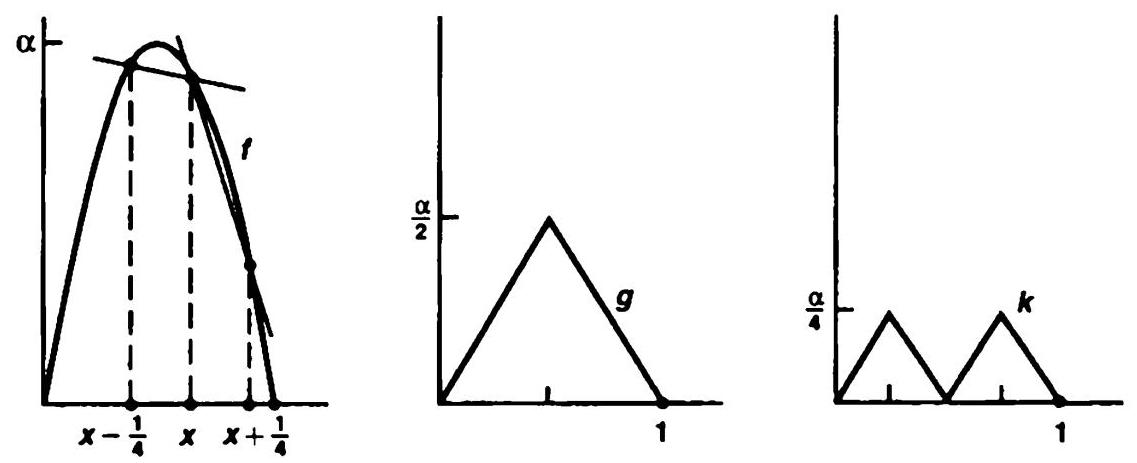
\includegraphics[width=1.0\textwidth]{images/49.1.jpg}
\end{center}
\hspace*{3em} 

Figure 49.1
\end{example}

Now we prove the following facts about the set \({U}_{n}\) :

(1) \(\bigcap {U}_{n}\) consists of \idx{nowhere-differentiable function}s. Let \(f \in  \bigcap {U}_{n}\) . We shall prove that given \(x\) in \(\left\lbrack  {0,1}\right\rbrack\) , the limit

\[
\lim {\Delta f}\left( {x,h}\right)
\]

does not exist: Given \(n\) , the fact that \(f\) belongs to \({U}_{n}\) means that we can find a number \({h}_{n}\) with \(0 < {h}_{n} \leq  1/n\) such that

\[
{\Delta f}\left( {x,{h}_{n}}\right)  > n\text{ . }
\]

Then the sequence \(\left( {h}_{n}\right)\) converges to zero, but the sequence \(\left( {{\Delta f}\left( {x,{h}_{n}}\right) }\right)\) does not converge. As a result, \(f\) is not differentiable at \(x\) .

(2) \({U}_{n}\) is open in \(\mathcal{C}\) . Suppose that \(f \in  {U}_{n}\) ; we find a \(\delta\) -neighborhood of \(f\) that is contained in \({U}_{n}\) . Because \(f \in  {U}_{n}\) , there is a number \(h\) with \(0 < h \leq  1/n\) such that \({\Delta }_{h}f > n\) . Set \(M = {\Delta }_{h}f\) , and let

\[
\delta  = h\left( {M - n}\right) /4
\]

We assert that if \(g\) is a function with \(\rho \left( {f,g}\right)  < \delta\) , then

\[
{\Delta g}\left( {x,h}\right)  \geq  \frac{1}{2}\left( {M + n}\right)  > n
\]

for all \(x \in  I\) , so that \(g \in  {U}_{n}\) .

To prove the assertion, let us first assume that \({\Delta f}\left( {x,h}\right)\) is equal to the quotient \(\left| {f\left( {x + h}\right)  - f\left( x\right) }\right| /h\) . We compute

\[
\left| {\frac{f\left( {x + h}\right)  - f\left( x\right) }{h} - \frac{g\left( {x + h}\right)  - g\left( x\right) }{h}}\right|  =
\]

\[
\left( {1/h}\right) \left| {\left\lbrack  {f\left( {x + h}\right)  - g\left( {x + h}\right) }\right\rbrack   - \left\lbrack  {f\left( x\right)  - g\left( x\right) }\right\rbrack  }\right|  \leq  {2\delta }/h = \left( {M - n}\right) /2.
\]

If the first difference quotient is at least \(M\) in absolute value, then the second is in absolute value at least

\[
M - \frac{1}{2}\left( {M - n}\right)  = \frac{1}{2}\left( {M + n}\right) .
\]

A similar remark applies if \({\Delta f}\left( {x,h}\right)\) equals the other difference quotient.

(3) \({U}_{n}\) is dense in \(\mathcal{C}\) . We must show that given \(f\) in \(\mathcal{C}\) , given \(\epsilon  > 0\) , and given \(n\) , we can find an element \(g\) of \({U}_{n}\) within \(\epsilon\) of \(f\) .

Choose \(\alpha  > n\) . We shall construct \(g\) as a "\idx{Piecewise linear function} piecewise-linear" function, that is, a function whose graph is a broken line segment; each line segment in the graph of \(g\) will have slope at least \(\alpha\) in absolute value. It follows at once that such a function \(g\) belongs to \({U}_{n}\) . For let

\[
0 = {x}_{0} < {x}_{1} < {x}_{2} < \cdots  < {x}_{k} = 1
\]

be a partition of the interval \(\left\lbrack  {0,1}\right\rbrack\) such that the restriction of \(g\) to each subinterval \({I}_{i} = \left\lbrack  {{x}_{i - 1},{x}_{i}}\right\rbrack\) is a linear function. Then choose \(h\) so that \(h \leq  1/n\) and

\[
h \leq  \frac{1}{2}\min \left\{  {\left| {{x}_{i} - {x}_{i - 1}}\right| ;i = 1,\ldots ,k}\right\}  .
\]

If \(x\) is in \(\left\lbrack  {0,1}\right\rbrack\) , then \(x\) belongs to some subinterval \({I}_{i}\) . If \(x\) belongs to the first half of the subinterval \({I}_{i}\) , then \(x + h\) belongs to \({I}_{i}\) and \(\left( {g\left( {x + h}\right)  - g\left( x\right) }\right) /h\) equals the slope of the linear function \(g \mid  {I}_{i}\) Similarly, if \(x\) belongs to the second half of \({I}_{i}\) , then \(x - h\) belongs to \({I}_{i}\) and \(\left( {g\left( {x - h}\right)  - g\left( x\right) }\right) /\left( {-h}\right)\) equals the slope of \(g \mid  {I}_{i}\) . In either case, \({\Delta g}\left( {x,h}\right)  \geq  \alpha\) , so \(g \in  {U}_{n}\) , as desired.

Now given \(f,\epsilon\) , and \(\alpha\) , we must show how to construct the desired piecewise-linear function \(g\) . First, we use uniform continuity of \(f\) to choose a partition of the interval

\[
0 = {t}_{0} < {t}_{1} < \cdots  < {t}_{m} = 1
\]

having the property that \(f\) varies by at most \(\epsilon /4\) on each subinterval \(\left\lbrack  {{t}_{i - 1},{t}_{i}}\right\rbrack\) of this partition. For each \(i = 1,\ldots ,m\) , choose a point \({a}_{i} \in  \left( {{t}_{i - 1},{t}_{i}}\right)\) . We then define a piecewise-linear function \({g}_{1}\) by the equations

\[
{g}_{1}\left( x\right)  = \left\{  \begin{array}{ll} f\left( {t}_{i - 1}\right) & \text{ for }x \in  \left\lbrack  {{t}_{i - 1},{a}_{i}}\right\rbrack  , \\  f\left( {t}_{i - 1}\right)  + {m}_{i}\left( {x - {a}_{i}}\right) & \text{ for }x \in  \left\lbrack  {{a}_{i},{t}_{l}}\right\rbrack  , \end{array}\right.
\]

where \({m}_{i} = \left( {f\left( {t}_{i}\right)  - f\left( {t}_{i - 1}\right) }\right) /\left( {{t}_{i} - {a}_{i}}\right)\) . The graphs of \(f\) and \({g}_{1}\) are pictured in Figure 49.2.

\begin{center}
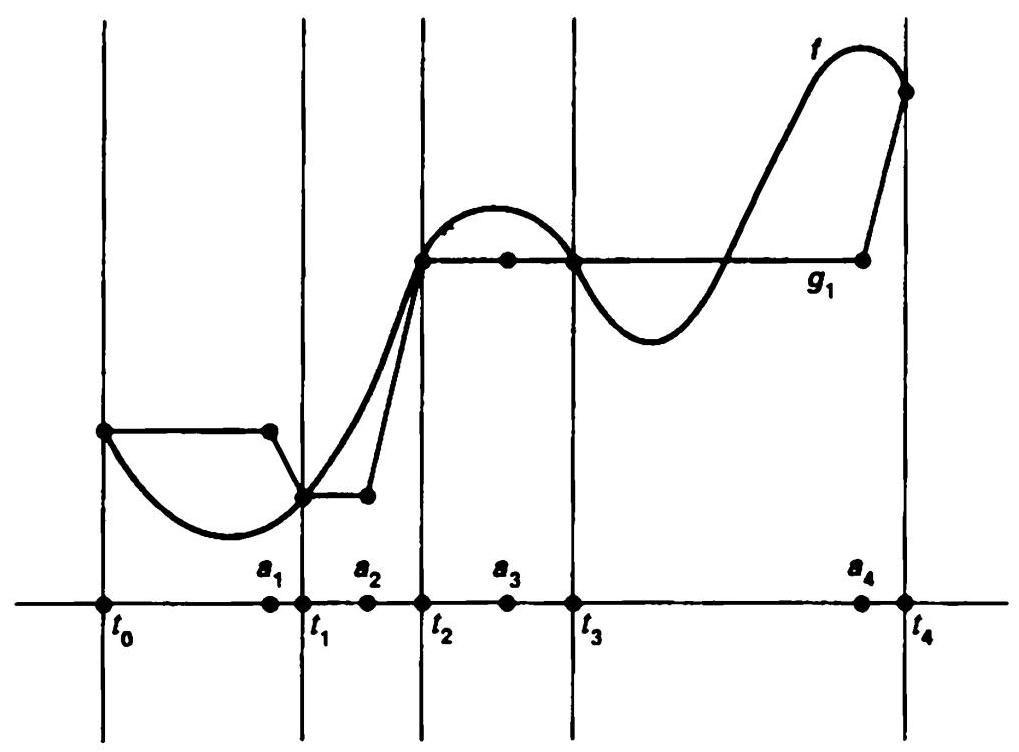
\includegraphics[width=0.9\textwidth]{images/49.2.jpg}
\end{center}
\hspace*{3em} 

Figure 49.2

We have some freedom of choice in choosing the point \({a}_{i}\) . If \(f\left( {t}_{i}\right)  \neq  f\left( {t}_{i - 1}\right)\) , we require \({a}_{i}\) to be close enough to \({t}_{i}\) that

\[
{t}_{i} - {a}_{i} < \frac{\left| f\left( {t}_{i}\right)  - f\left( {t}_{i - 1}\right) \right| }{\alpha }
\]

Then the graph of \({g}_{1}\) will consist entirely of line segments of slope zero and line segments of slope at least \(\alpha\) in absolute value.

Furthermore, we assert that \(\rho \left( {{g}_{1},f}\right)  \leq  \epsilon /2\) . On the interval \({I}_{i}\) , both \({g}_{1}\left( x\right)\) and \(f\left( x\right)\) vary by at most \(\epsilon /4\) from \(f\left( {t}_{i - 1}\right)\) ; therefore, they are within \(\epsilon /2\) of each other. Then \(\rho \left( {{g}_{1},f}\right)  = \max \left\lbrack  \left| {{g}_{1}\left( x\right)  - f\left( x\right) }\right| \right\}   \leq  \epsilon /2\) .

\begin{center}
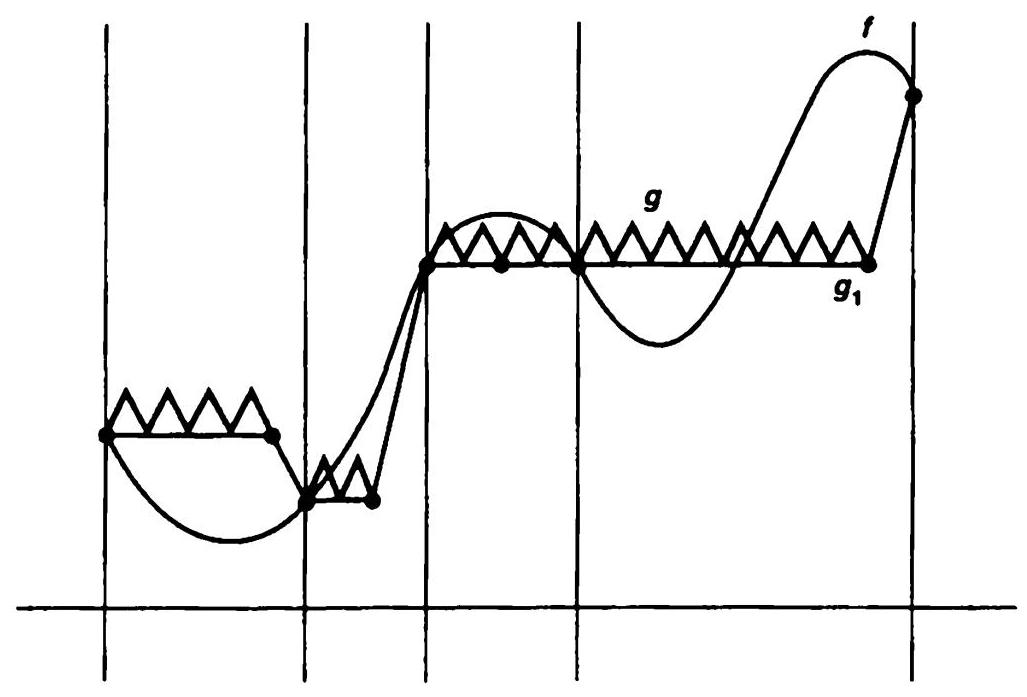
\includegraphics[width=0.9\textwidth]{images/49.3.jpg}
\end{center}
\hspace*{3em} 

Figure 49.3

The function \({g}_{1}\) is not yet the function we want. We now define a function \(g\) by replacing each horizontal line segment in the graph of \({g}_{1}\) by a "sawtooth" graph that lies within \(\epsilon /2\) of the graph of \({g}_{1}\) and has the property that each edge of the sawtooth has slope at least \(\alpha\) in absolute value. We leave this part of the construction to you. The result is the desired piecewise-linear function \(g\) . See Figure 49.3.

You may find this proof frustrating, in that it seems so abstract and nonconstructive. Implicit in the proof, however, is a procedure for constructing a specific sequence \({f}_{n}\) of piecewise-linear functions that converges uniformly to the nowhere-differentiable function \(f\) . And defining the function \(f\) in this way is just as constructive as the usual definition of the sine function, for instance, as the limit of an infinite senes.
\end{proof}
\section*{Exercises}

1. Check the stated properties of the functions \(f,g\) , and \(k\) of Example 1.

2. Given \(n\) and \(\epsilon\) , define a continuous function \(f : I \rightarrow  \mathbb{R}\) such that \(f \in  {U}_{n}\) and \(\left| {f\left( x\right) }\right|  \leq  \epsilon\) for all \(x\) .

\section*{§ 50 Introduction to Dimension Theory}

We showed in \(§{36}\) that if \(X\) is a compact manifold, then \(X\) can be imbedded in \({\mathbb{R}}^{N}\) for some positive integer \(N\) . In this section, we generalize this theorem to arbitrary compact metrizable spaces

We shall define, for an arbitrary topological space \(X\) , a notion of topological dimension. It is the "\idx{covering dimension}" originally defined by Lebesgue We shall prove that each compact subset of \({\mathbb{R}}^{m}\) has topological dimension at most \(m\) . We shall also prove that the topological dimension of any compact \(m\) -manifold is at most \(m\) . (It is, in fact, precisely \(m\) , but this we shall not prove.)

The major theorem of this section is the theorem, due to K. Menger and G. Nöbel-ing, that any compact metrizable space of topological dimension \(m\) can be imbedded in \({\mathbb{R}}^{N}\) for \(N = {2m} + 1\) . The proof is an application of the Baire theorem. It follows that every compact \(m\) -manifold can be imbedded in \({\mathbb{R}}^{{2m} + 1}\) . It follows also that a compact metrizable space can be imbedded in \({\mathbb{R}}^{N}\) for some \(N\) if and only if it has finite topological dimension.

Much of what we shall do holds without requiring the space in question to be compact. But we shall restrict ourselves to that case whenever it is convenient to do so. Generalizations to the noncompact case are given in the exercises.

\begin{definition} A collection \(\mathcal{A}\) of subsets of the space \(X\) is said to have \idx{Order of a covering} order \(m + 1\) if some point of \(X\) lies in \(m + 1\) elements of \(\mathcal{A}\) , and no point of \(X\) lies in more than \(m + 1\) elements of \(\mathcal{A}\) .
\end{definition}

Now we define what we mean by the topological dimension of a space \(X\) Recall that given a collection \(\mathcal{A}\) of subsets of \(X\) , a collection \(\mathcal{B}\) is said to refine \(\mathcal{A}\) , or to be a refinement of \(\mathcal{A}\) , if for each element \(B\) of \(\mathcal{B}\) there is an element \(A\) of \(\mathcal{A}\) such that \(B \subset  A\) .

\begin{definition} A space \(X\) is said to be \idx{finite dimensional} if there is some integer \(m\) such that for every open covering \(\mathcal{A}\) of \(X\) , there is an open covering \(\mathcal{B}\) of \(X\) that refines \(\mathcal{A}\) and has order at most \(m + 1\) . The topological dimension of \(X\) is defined to be the smallest value of \(m\) for which this statement holds; we denote it by \(\dim X\) .
\end{definition}

\begin{example} Any compact subspace \(X\) of \(\mathbb{R}\) has topological dimension at most 1. We begin by defining an open covering of \(\mathbb{R}\) of order 2 Let \({\mathcal{A}}_{1}\) denote the collection of all open intervals of the form \(\left( {n,n + 1}\right)\) in \(\mathbb{R}\) , where \(n\) is an integer. Let \({\mathcal{A}}_{0}\) denote the collection of all open intervals of the form \(\left( {n - 1/2,n + 1/2}\right)\) , for \(n\) an integer. Then \(\mathcal{A} = {\mathcal{A}}_{0} \cup  {\mathcal{A}}_{1}\) is an open covering of \(\mathbb{R}\) by sets of diameter one Because no two elements of \({\mathcal{A}}_{0}\) intersect, and no two elements of \({\mathcal{A}}_{1}\) intersect, \(\mathcal{A}\) has order 2 .

Now let \(X\) be a compact subspace of \(\mathbb{R}\) . Given a covering \(\mathcal{C}\) of \(X\) by sets open in \(X\) , this covering has a positive Lebesgue number \(\delta\) . This means that any collection of subsets of \(X\) that have diameter less than \(\delta\) is automatically a refinement of \(\mathcal{C}\) . Consider the homeomorphism \(f\mathbb{R} \rightarrow  \mathbb{R}\) defined by \(f\left( x\right)  = \left( {\frac{1}{2}\delta }\right) x\) The images under \(f\) of the elements of the collection \(\mathcal{A}\) form an open covering of \(\mathbb{R}\) of order 2 whose elements have diameter \(\frac{1}{2}\delta\) ; their intersections with \(X\) form the required open covering of \(X\) .
\end{example}

\begin{example} The interval \(X = \left\lbrack  {0,1}\right\rbrack\) has topological dimension 1. We know that \(\dim X \leq  1\) . To show equality holds, let \(\mathcal{A}\) be the covering of \(X\) by the sets \(\left\lbrack  {0,1}\right\rbrack\) and \((0,1\rbrack\) . We show that if \(\mathcal{B}\) is any open covering of \(X\) that refines \(\mathcal{A}\) , then \(\mathcal{B}\) has order at least 2 . Since \(\mathcal{B}\) refines \(\mathcal{A}\) , it must contain more than one element Let \(U\) be one of the elements of \(\mathcal{B}\) and let \(V\) be the union of the others. If \(\mathcal{B}\) had order 1, then the sets \(U\) and \(V\) would be disjoint and would thus form a separation of \(X\) . We conclude that \(\mathcal{B}\) has order at least 2 .
\end{example}

\begin{example} Any compact subspace \(X\) of \({\mathbb{R}}^{2}\) has topological dimension at most 2. To prove this fact, we construct a certain open covering \(\mathcal{A}\) of \({\mathbb{R}}^{2}\) that has order 3 We begin by defining \({\mathcal{A}}_{2}\) to be the collection of all open unit squares in \({\mathbb{R}}^{2}\) of the following form:

\[
{\mathcal{A}}_{2} = \{ \left( {n,n + 1}\right)  \times  \left( {m,m + 1}\right)  \mid  n,m\text{ integers }\}
\]

Note that the elements of \({\mathcal{A}}_{2}\) are disjoint. Then, we define a collection \({\mathcal{A}}_{1}\) by taking each (open) edge \(e\) of one of these squares,

\[
e = \{ n\}  \times  \left( {m,m + 1}\right) \;\text{ or }\;e = \left( {n,n + 1}\right)  \times  \{ m\} ,
\]

and expanding it slightly to an open set \({U}_{e}\) of \({\mathbb{R}}^{2}\) , being careful to ensure that if \(e \neq  {e}^{\prime }\) , the sets \({U}_{e}\) and \({U}_{{e}^{\prime }}\) are disjoint We also choose each \({U}_{e}\) so that its diameter is at most 2 . Finally, we define \({\mathcal{A}}_{0}\) to be the collection consisting of all open balls of radius \(\frac{1}{2}\) about the points \(n \times  m\) . See Figure 50.1

The collection of open sets \(\mathcal{A} = {\mathcal{A}}_{2} \cup  {\mathcal{A}}_{1} \cup  {\mathcal{A}}_{0}\) covers \({\mathbb{R}}^{2}\) Each of its elements has diameter at most 2 . And it has order 3, since no point of \({\mathbb{R}}^{2}\) can lie in more than one set from each \({\mathcal{A}}_{1}\) .

\begin{center}
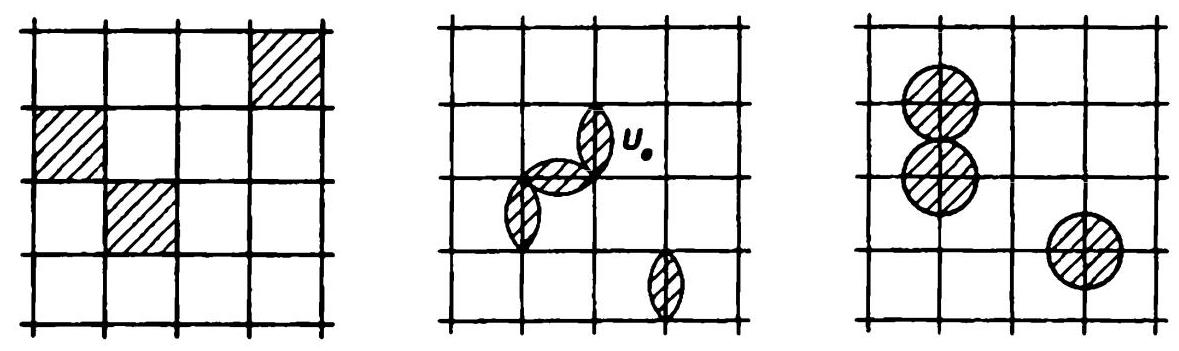
\includegraphics[width=1.0\textwidth]{images/50.1.jpg}
\end{center}
\hspace*{3em} 

Figure 50.1

Now let \(X\) be a compact subspace of \({\mathbb{R}}^{2}\;\) Given an open covering of \(X\) , it has a positive Lebesgue number \(\delta\) . Consider the homeomorphism \(f : {\mathbb{R}}^{2} \rightarrow  {\mathbb{R}}^{2}\) defined by the equation \(f\left( x\right)  = \left( {\delta /3}\right) x\) . The images under \(f\) of the open sets of the collection \(\mathcal{A}\) form an open covering of \({\mathbb{R}}^{2}\) by sets of diameter less than \(\delta\) , their intersections with \(X\) form the required open covering of \(X\) .

We shall generalize this result to compact subsets of \({\mathbb{R}}^{n}\) shortly.

Some basic facts about topological dimension are given in the following theorems:

\begin{theorem} Let \(X\) be a space having finite dimension. If \(Y\) is a closed subspace of \(X\) , then \(Y\) has finite dimension and \(\dim Y \leq  \dim X\) .
\end{theorem}

\begin{proof}Let \(\dim X = m\) . Let \(\mathcal{A}\) be a covering of \(Y\) by sets open in \(Y\) . For each \(A \in  \mathcal{A}\) , choose an open set \({A}^{\prime }\) of \(X\) such that \({A}^{\prime } \cap  Y = A\) . Cover \(X\) by the open sets \({A}^{\prime }\) , along with the open set \(X - Y\) . Let \(\mathcal{B}\) be a refinement of this covering that is an open covering of \(X\) and has order at most \(m + 1\) . Then the collection
\[
\{ B \cap  Y \mid  B \in  \mathcal{B}\}
\]

is a covering of \(Y\) by sets open in \(Y\) , it has order at most \(m + 1\) , and it refines \(\mathcal{A}\) .
\end{proof}
\begin{theorem} Let \(X = Y \cup  Z\) , where \(Y\) and \(Z\) are closed subspaces of \(X\) having finite topological dimension. Then

\[
\dim X = \max \{ \dim Y,\dim Z\} .
\]
\end{theorem}

\begin{proof}Let \(m = \max \{ \dim Y,\dim Z\}\) . We shall show that \(X\) is finite dimensional and has topological dimension at most \(m\) . It then follows from the preceding theorem that \(X\) has topological dimension precisely \(m\) .
Step 1. If \(\mathcal{A}\) is an open covering of \(X\) , we say that \(\mathcal{A}\) has order at most \(m + 1\) at points of \(Y\) provided no point of \(Y\) lies in more than \(m + 1\) elements of \(\mathcal{A}\) .

We show that if \(\mathcal{A}\) is an open covering of \(X\) , then there is an open covering of \(X\) that refines \(\mathcal{A}\) and has order at most \(m + 1\) at points of \(Y\) .

To prove this fact, consider the collection

\[
\{ A \cap  Y \mid  A \in  \mathcal{A}\} .
\]

It is an open covering of \(Y\) , so it has a refinement \(\mathcal{B}\) that is an open covering of \(Y\) and has order at most \(m + 1\) . Given \(B \in  \mathcal{B}\) , choose an open set \({U}_{B}\) of \(X\) such that \({U}_{B} \cap  Y = B\) . Choose also an element \({A}_{B}\) of \(\mathcal{A}\) such that \(B \subset  {A}_{B}\) . Let \(\mathcal{C}\) be the collection consisting of all the sets \({U}_{B} \cap  {A}_{B}\) , for \(B \in  \mathcal{B}\) , along with all the sets \(A - Y\) , for \(A \in  \mathcal{A}\) . Then \(\mathcal{C}\) is the desired open covering of \(X\) .

Step 2. Now let \(\mathcal{A}\) be an open covering of \(X\) . We construct an open covering \(\mathcal{D}\) of \(X\) that refines \(\mathcal{A}\) and has order at most \(m + 1\) . Let \(\mathcal{B}\) be an open covering of \(X\) refining \(\mathcal{A}\) that has order at most \(m + 1\) at points of \(Y\) . Then let \(\mathcal{C}\) be an open covering of \(X\) refining \(\mathcal{B}\) that has order at most \(m + 1\) at points of \(Z\) .

We form a new covering \(\mathcal{D}\) of \(X\) as follows: Define \(f : \mathcal{C} \rightarrow  \mathcal{B}\) by choosing for each \(C \in  \mathcal{C}\) an element \(f\left( C\right)\) of \(\mathcal{B}\) such that \(C \subset  f\left( C\right)\) . Given \(B \in  \mathcal{B}\) , define \(D\left( B\right)\) to be the union of all those elements \(C\) of \(\mathcal{C}\) for which \(f\left( C\right)  = B\) . (Of course, \(D\left( B\right)\) is empty if \(B\) is not in the image of \(f\) .) Let \(\mathcal{D}\) be the collection of all the sets \(D\left( B\right)\) , for \(B \in  \mathcal{B}\) .

Now \(\mathcal{D}\) refines \(\mathcal{B}\) , because \(D\left( B\right)  \subset  B\) for each \(B\) ; therefore, \(\mathcal{D}\) refines \(\mathcal{A}\) . Also, \(\mathcal{D}\) covers \(X\) because \(\mathcal{C}\) covers \(X\) and \(C \subset  D\left( {f\left( C\right) }\right)\) for each \(C \in  \mathcal{C}\) . We show that \(\mathcal{D}\) has order at most \(m + 1\) . Suppose \(x \in  D\left( {B}_{1}\right)  \cap  \cdots  \cap  D\left( {B}_{k}\right)\) , where the sets \(D\left( {B}_{i}\right)\) are distinct. We wish to prove that \(k \leq  m + 1\) . Note that the sets \({B}_{1},\ldots ,{B}_{k}\) must be distinct because the sets \(D\left( {B}_{i}\right)\) are. Because \(x \in  D\left( {B}_{i}\right)\) , we can choose for each \(i\) , a set \({C}_{i} \in  \mathcal{C}\) such that \(x \in  {C}_{i}\) and \(f\left( {C}_{i}\right)  = {B}_{i}\) . The sets \({C}_{i}\) are distinct because the sets \({B}_{i}\) are. Furthermore,

\[
x \in  \left\lbrack  {{C}_{1} \cap  \cdots  \cap  {C}_{k}}\right\rbrack   \subset  \left\lbrack  {D\left( {B}_{1}\right)  \cap  \cdots  \cap  D\left( {B}_{k}\right) }\right\rbrack   \subset  \left\lbrack  {{B}_{1} \cap  \cdots  \cap  {B}_{k}}\right\rbrack  .
\]

If \(x\) happens to lie in \(Y\) , then \(k \leq  m + 1\) because \(\mathcal{B}\) has order at most \(m + 1\) at points of \(Y\) ; and if \(x\) is in \(Z\) , then \(k \leq  m + 1\) because \(\mathcal{C}\) has order at most \(m + 1\) at points of \(z\) .
\end{proof}
\begin{corollary} Let \(X = {Y}_{1} \cup  \cdots  \cup  {Y}_{k}\) , where each \({Y}_{1}\) is a closed subspace of \(X\) and is finite dimensional. Then

\[
\dim X = \max \left\{  {\dim {Y}_{1},\ldots ,\dim {Y}_{k}}\right\}
\]
\end{corollary}
\end{example}

\begin{example} Every compact 1-manifold \(X\) has topological dimension 1. The space \(X\) can be written as a finite union of spaces that are homeomorphic to the unit interval \(\lbrack 0,1\}\) ; then the preceding corollary applies
\end{example}

\begin{example} Every compact 2-manifold \(X\) has topological dimension at most 2. The space \(X\) can be written as a finite union of spaces that are homeomorphic to the closed unit ball in \({\mathbb{R}}^{2}\) , then the preceding corollary applies.
\end{example}

An obvious question occurs at this point: Does a compact 2-manifold have topological dimension precisely 27 The answer is "yes," but the proof is not easy; it requires the tools of algebraic topology. We will prove in Part II of this book that every closed triangular region in \({\mathbb{R}}^{2}\) has topological dimension at least 2. (See §55.) It then follows that any compact subspace of \({\mathbb{R}}^{2}\) that contains a closed triangular region has topological dimension 2, from which it follows that every compact 2-manifold has topological dimension 2

\begin{example} An \idx{arc} \(A\) is a space homeomorphic to the closed unit interval; the end points of \(A\) are the points \(p\) and \(q\) such that \(A - \{ p\}\) and \(A - \{ q\}\) are connected \(A\) (finite) \idx{linear graph} \(G\) is a Hausdorff space that is written as the union of finitely many arcs, each pair of which intersect in at most a common end point. The arcs in the collection are called the edges of \(G\) , and the end points of the arcs are called the vertices of \(G\) Each edge of \(G\) , being compact, is closed in \(G\) ; the preceding corollary tells us that \(G\) has topological dimension 1
\end{example}

Two particular linear graphs are sketched in Figure 50.2. The first is a diagram of the familiar "gas-water-electricity problem"; the second is called the "complete graph on five vertices." Neither of them can be imbedded in \({\mathbb{R}}^{2}\) . Although this fact is "intuitively obvious," it is highly nontrivial to prove We shall give a proof in §64. are in \idx{general position} For if four of these points belonged to a single plane \({Ax} + {By} +\)  \({Cz} = D\) , then the polynomial equation

\[
{At} + B{t}^{2} + C{t}^{3} = D
\]

\begin{center}
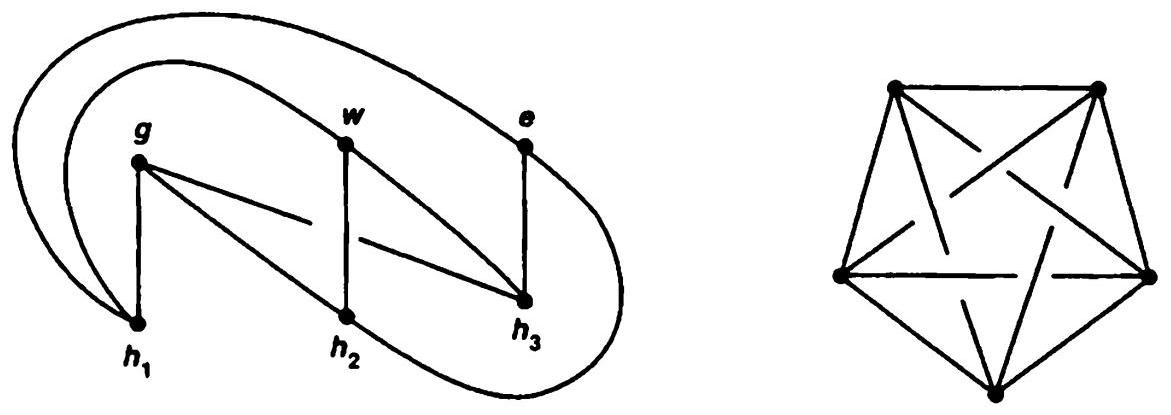
\includegraphics[width=1.0\textwidth]{images/50.2.jpg}
\end{center}
\hspace*{3em} 

Figure 50.2

\begin{example} Every finite linear graph can be imbedded in \({\mathbb{R}}^{3}\) . The proof involves the notion of "general position." A set \(S\) of points of \({\mathbb{R}}^{3}\) is said to be in general posinon if no three of the points of \(S\) are collinear and no four of them are coplanar. It is easy to find such a set of points. For example, the points of the curve

\[
S = \left\{  {\left( {t,{t}^{2},{t}^{3}}\right)  \mid  t \in  \mathbb{R}}\right\}
\]

would have four distinct real roots \({}^{1}\) And if three of these points belonged to a single line, we could take an additional point of \(S\) and obtain four points that lie on a plane.

Now, given a finite linear graph \(G\) , with vertices \({v}_{1},\ldots ,{v}_{n}\) , let us choose a set \(\left\{  {{\mathbf{z}}_{1},\ldots ,{\mathbf{z}}_{n}}\right\}\) of points of \({\mathbb{R}}^{3}\) that is in general position. Define a map \(f : G \rightarrow  {\mathbb{R}}^{3}\) by letting \(f\) map the vertex \({v}_{i}\) to the point \({\mathbf{z}}_{i}\) , and map the edge joining \({v}_{i}\) and \({v}_{j}\) homeo-morphically onto the line segment joining \({\mathbf{z}}_{i}\) and \({\mathbf{z}}_{j}\) . Now each edge of \(G\) is closed in \(G\) It follows that \(f\) is continuous, by the pasting lemma. We show that \(f\) is injective, from which it follows that \(f\) is an imbedding. Let \(e = {v}_{i}{v}_{j}\) and \({e}^{\prime } = {v}_{k}{v}_{m}\) be two edges of \(G\) If they have no vertex in common, then the line segments \(f\left( e\right)\) and \(f\left( {e}^{\prime }\right)\) are disjoint, for otherwise the points \({\mathbf{z}}_{i},{\mathbf{z}}_{j},{\mathbf{z}}_{k},{\mathbf{z}}_{m}\) would be coplanar. And if \(e\) and \({e}^{\prime }\) have a vertex in common, so that \(i = k\) , say, then the line segments \(f\left( e\right)\) and \(f\left( {e}^{\prime }\right)\) intersect only in the point \({\mathbf{z}}_{i} = {\mathbf{z}}_{k}\) , for otherwise \({\mathbf{z}}_{i},{\mathbf{z}}_{j}\) , and \({\mathbf{z}}_{m}\) would be collinear.
\end{example}

Now we prove our general imbedding theorem, to the effect that every compact metrizable space of topological dimension \(m\) can be imbedded in \({\mathbb{R}}^{{2m} + 1}\) . This theorem is another "deep" theorem; it is not at all obvious, for instance, why \({2m} + 1\) should be the crucial dimension. That will come out in the course of the proof.

To prove the imbedding theorem, we shall need to generalize the notion of general position to \({\mathbb{R}}^{N}\) . This involves a bit of the analytic geometry of \({\mathbb{R}}^{N}\) , which is nothing more than the usual linear algebra of \({\mathbb{R}}^{N}\) translated into somewhat different language.

\begin{definition} A set \(\left\{  {{\mathbf{x}}_{0},\ldots ,{\mathbf{x}}_{k}}\right\}\) of points of \({\mathbb{R}}^{N}\) is said to be \idx{geometrically independent}, or \idx{affinely independent}, if the equations

\[
\mathop{\sum }\limits_{{i = 0}}^{k}{a}_{i}{\mathbf{x}}_{i} = \mathbf{0}\;\text{ and }\;\mathop{\sum }\limits_{{i = 0}}^{k}{a}_{i} = 0
\]

hold only if each \({a}_{t} = 0\) .
\end{definition}

Obviously, a set consisting of only one point is geometrically independent. But what does geometric independence mean in general? If we solve the second equation for \({a}_{0}\) and plug the answer into the first equation, we see that this definition is equivalent to the statement that the equation

\[
\mathop{\sum }\limits_{{i = 1}}^{k}{a}_{i}\left( {{\mathbf{x}}_{i} - {\mathbf{x}}_{0}}\right)  = \mathbf{0}
\]

holds only if each \({a}_{i} = 0\) . This is just the definition of linear independence for the set of vectors \({\mathbf{x}}_{1} - {\mathbf{x}}_{0},\ldots ,{\mathbf{x}}_{k} - {\mathbf{x}}_{0}\) of the vector space \({\mathbb{R}}^{N}\) . This gives us something to visualize: Any two distinct points form a geometrically independent set. Three points form a geometrically independent set if they are not collinear. Four points in \({\mathbb{R}}^{3}\) form a geometrically independent set if they are not coplanar. And so on.

It follows from these remarks that the points

\[
\mathbf{0} = \left( {0,0,\ldots ,0}\right) \text{ , }
\]

\[
{\epsilon }_{1} = \left( {1,0,\ldots ,0}\right) \text{ , }
\]

\[
{\epsilon }_{N} = \left( {0,0,\ldots ,1}\right)
\]

are geometrically independent in \({\mathbb{R}}^{N}\) . It also follows that any geometrically independent set of points in \({\mathbb{R}}^{N}\) contains no more than \(N + 1\) points

\begin{definition} Let \(\left\{  {{\mathbf{x}}_{0},\ldots ,{\mathbf{x}}_{k}}\right\}\) be a set of points of \({\mathbb{R}}^{N}\) that is geometrically independent. The plane \(P\) determined by these points is defined to be the set of all points \(\mathbf{x}\) of \({\mathbb{R}}^{N}\) such that

\[
\mathbf{x} = \mathop{\sum }\limits_{{i = 0}}^{k}{t}_{i}{\mathbf{x}}_{i},\;\text{ where }\mathop{\sum }\limits_{{i = 0}}^{k}{t}_{i} = 1.
\]
\end{definition}

It is simple algebra to check that \(P\) can also be expressed as the set of all points \(\mathbf{x}\) such that

(*)
\[
\mathbf{x} = {\mathbf{x}}_{0} + \mathop{\sum }\limits_{{i = 1}}^{k}{a}_{i}\left( {{\mathbf{x}}_{i} - {\mathbf{x}}_{0}}\right)
\]

for some scalars \({a}_{1},\ldots ,{a}_{k}\) . Thus \(P\) can be described not only as "the plane determined by the points \({\mathbf{x}}_{0},\ldots ,{\mathbf{x}}_{k}\) ," but also as "the plane passing through the point \({\mathbf{x}}_{0}\) parallel to the vectors \({\mathbf{x}}_{1} - {\mathbf{x}}_{0},\ldots ,{\mathbf{x}}_{k} - {\mathbf{x}}_{0}\) ."

Consider now the homeomorphism \(T : {\mathbb{R}}^{N} \rightarrow  {\mathbb{R}}^{N}\) defined by the equation \(T\left( \mathbf{x}\right)  = \mathbf{x} - {\mathbf{x}}_{0}\) . It is called a translation of \({\mathbb{R}}^{N}\) . Expression (*) shows that this map carries the plane \(P\) onto the vector subspace \({V}^{k}\) of \({\mathbb{R}}^{N}\) having as basis the vectors \({\mathbf{x}}_{1} - {\mathbf{x}}_{0},\ldots ,{\mathbf{x}}_{k} - {\mathbf{x}}_{0}\) . For this reason, we often call \(P\) a \(k\) -plane in \({\mathbb{R}}^{N}\) .

Two facts follow at once: First, if \(k < N\) , the \(k\) -plane \(P\) necessarily has empty interior in \({\mathbb{R}}^{N}\) (because \({V}^{k}\) does). And second, if \(\mathbf{y}\) is any point of \({\mathbb{R}}^{N}\) not lying in \(P\) , then the set

\[
\left\{  {{\mathbf{x}}_{0},\ldots ,{\mathbf{x}}_{k},\mathbf{y}}\right\}
\]

is geometrically independent. For if \(\mathbf{y} \notin  P\) , then \(T\left( \mathbf{y}\right)  = \mathbf{y} - {\mathbf{x}}_{0}\) is not in \({V}^{k}\) . By a standard theorem of linear algebra, the vectors \(\left\{  {{\mathbf{x}}_{1} - {\mathbf{x}}_{0},\ldots ,{\mathbf{x}}_{k} - {\mathbf{x}}_{0},\mathbf{y} - {\mathbf{x}}_{0}}\right\}\) are linearly independent, from which our result follows.

\begin{definition} A set \(A\) of points of \({\mathbb{R}}^{N}\) is said to be in general position in \({\mathbb{R}}^{N}\) if every subset of \(A\) containing \(N + 1\) or fewer points is geometrically independent.
\end{definition}

In the case of \({\mathbb{R}}^{3}\) , this is the same as the definition given earlier, as you can check.

\begin{lemma} Given a finite set \(\left\{  {{\mathbf{x}}_{1},\ldots ,{\mathbf{x}}_{n}}\right\}\) of points of \({\mathbb{R}}^{N}\) and given \(\delta  > 0\) , there exists a set \(\left\{  {{\mathbf{y}}_{1},\ldots ,{\mathbf{y}}_{n}}\right\}\) of points of \({\mathbb{R}}^{N}\) in general position in \({\mathbb{R}}^{N}\) , such that \(\left| {{\mathbf{x}}_{i} - {\mathbf{y}}_{i}}\right|  < \delta\) for all \(i\) .
\end{lemma}

\begin{proof}We proceed by induction. Set \({\mathbf{y}}_{1} = {\mathbf{x}}_{1}\) . Suppose that we are given \({\mathbf{y}}_{1},\ldots ,{\mathbf{y}}_{p}\) in general position in \({\mathbb{R}}^{N}\) . Consider the set of all planes in \({\mathbb{R}}^{N}\) determined by subsets of \(\left\{  {{\mathbf{y}}_{1},\ldots ,{\mathbf{y}}_{p}}\right\}\) that contain \(N\) or fewer elements. Every such subset is geometrically independent and determines a \(k\) -plane of \({\mathbb{R}}^{N}\) for some \(k \leq  N - 1\) . Each of these planes has empty interior in \({\mathbb{R}}^{N}\) Because there are only finitely many of them, their union also has empty interior in \({\mathbb{R}}^{N}\) . (Recall that \({\mathbb{R}}^{N}\) is a Bare space.) Choose \({\mathbf{y}}_{p + 1}\) to be a point of \({\mathbb{R}}^{N}\) within \(\delta\) of \({\mathbf{x}}_{p + 1}\) that does not lie in any of these planes. It follows at once that the set
\[
C = \left\{  {{\mathbf{y}}_{1},\ldots ,{\mathbf{y}}_{p},{\mathbf{y}}_{p + 1}}\right\}
\]

is in general position in \({\mathbb{R}}^{N}\) . For let \(D\) be any subset of \(C\) containing \(N + 1\) or fewer elements. If \(D\) does not contain \({\mathbf{y}}_{p + 1}\) , then \(D\) is geometrically independent by the induction hypothesis. If \(D\) does contain \({\mathbf{y}}_{p + 1}\) , then \(D - \left\{  {\mathbf{y}}_{p + 1}\right\}\) contains \(N\) or fewer points and \({\mathbf{y}}_{p + 1}\) is not in the plane determined by these points, by construction. Then as noted above, \(D\) is geometrically independent.
\end{proof}
\begin{theorem}[The imbedding theorem] Every compact metrizable space \(X\) of topological dimension \(m\) can be imbedded in \({\mathbb{R}}^{{2m} + 1}\) .
\end{theorem}

\begin{proof}Let \(N = {2m} + 1\) . Let us denote the square metric for \({\mathbb{R}}^{N}\) by
\[
\left| {\mathbf{x} - \mathbf{y}}\right|  = \max \left\{  {\left| {{x}_{i} - {y}_{i}}\right| ;i = 1,\ldots ,N}\right\}  .
\]

Then we can use \(\rho\) to denote the corresponding sup metric on the space \(\mathcal{C}\left( {X,{\mathbb{R}}^{N}}\right)\) ;

\[
\rho \left( {f,g}\right)  = \sup \{ \left| {f\left( x\right)  - g\left( x\right) }\right| ,x \in  X\} .
\]

The space \(\mathcal{C}\left( {X,{\mathbb{R}}^{N}}\right)\) is complete in the metric \(\rho\) , since \({\mathbb{R}}^{N}\) is complete in the square metric

Choose a metric \(d\) for the space \(X\) ; because \(X\) is compact, \(d\) is bounded. Given a continuous map \(f : X \rightarrow  {\mathbb{R}}^{N}\) , let us define

\[
\Delta \left( f\right)  = \sup \left\{  {\operatorname{diam}{f}^{-1}\left( {\{ z\} }\right)  \mid  z \in  f\left( X\right) }\right\}  .
\]

The number \(\Delta \left( f\right)\) measures how far \(f\) "deviates" from being injective; if \(\Delta \left( f\right)  = 0\) , each set \({f}^{-1}\left( {\{ z\} }\right)\) consists of exactly one point, so \(f\) is injective.

Now, given \(\epsilon  > 0\) , define \({U}_{\epsilon }\) to be the set of all those continuous maps \(f : X \rightarrow\)  \({\mathbb{R}}^{N}\) for which \(\Delta \left( f\right)  < \epsilon\) ; it consists of all those maps that "deviate" from being injective by less than \(\epsilon\) . We shall show that \({U}_{\epsilon }\) is both open and dense in \(\mathcal{C}\left( {X,{\mathbb{R}}^{N}}\right)\) . It follows that the intersection

\[
\mathop{\bigcap }\limits_{{n \in  {\mathbf{Z}}_{ + }}}{U}_{1/n}
\]

is dense in \(\mathcal{C}\left( {X,{\mathbb{R}}^{N}}\right)\) and is in particular nonempty.

If \(f\) is an element of this intersection, then \(\Delta \left( f\right)  < 1/n\) for every \(n\) . Therefore, \(\Delta \left( f\right)  = 0\) and \(f\) is injective. Because \(X\) is compact, \(f\) is an imbedding. Thus, the imbedding theorem is proved.

(1) \({U}_{\epsilon }\) is open in \(\mathcal{C}\left( {X,{\mathbb{R}}^{N}}\right)\) . Given an element \(f\) of \({U}_{\epsilon }\) , we wish to find some ball \({B}_{\rho }\left( {f,\delta }\right)\) about \(f\) that is contained in \({U}_{\epsilon }\) . First choose a number \(b\) such that \(\Delta \left( f\right)  < b < \epsilon\) . Note that if \(f\left( x\right)  = f\left( y\right)  = z\) , then \(x\) and \(y\) belong to the set \({f}^{-1}\left( {\{ z\} }\right)\) , so that \(d\left( {x,y}\right)\) must be less than \(b\) It follows that if we let \(A\) be the following subset of \(X \times  X\) ,

\[
A = \{ x \times  y \mid  d\left( {x,y}\right)  \geq  b\}
\]

then the function \(\left| {f\left( x\right)  - f\left( y\right) }\right|\) is positive on \(A\) . Now \(A\) is closed in \(X \times  X\) and therefore compact; hence the function \(\left| {f\left( x\right)  - f\left( y\right) }\right|\) has a positive minimum on \(A\) . Let

\[
\delta  = \frac{1}{2}\min \{ \left| {f\left( x\right)  - f\left( y\right) }\right| ;x \times  y \in  A\} .
\]

We assert that this value of \(\delta\) will suffice.

Suppose that \(g\) is a map such that \(\rho \left( {f,g}\right)  < \delta\) . If \(x \times  y \in  A\) , then \(\left| {f\left( x\right)  - f\left( y\right) }\right|  \geq\)  \({2\delta }\) by definition; since \(g\left( x\right)\) and \(g\left( y\right)\) are within \(\delta\) of \(f\left( x\right)\) and \(f\left( y\right)\) , respectively, we must have \(\left| {g\left( x\right)  - g\left( y\right) }\right|  > 0\) . Hence the function \(\left| {g\left( x\right)  - g\left( y\right) }\right|\) is positive on \(A\) . As a result, if \(x\) and \(y\) are two points such that \(g\left( x\right)  = g\left( y\right)\) , then necessarily \(d\left( {x,y}\right)  < b\) . We conclude that \({\Delta g} \leq  b < \epsilon\) , as desired.

(2) \({U}_{\epsilon }\) is dense in \(\mathcal{C}\left( {X,{\mathbb{R}}^{N}}\right)\) . This is the difficult part of the proof. We need to use the analytic geometry of \({\mathbb{R}}^{N}\) discussed earlier. Let \(f \in  \mathcal{C}\left( {X,{\mathbb{R}}^{N}}\right)\) . Given \(\epsilon  > 0\) and given \(\delta  > 0\) , we wish to find a function \(g \in  \mathcal{C}\left( {X,{\mathbb{R}}^{N}}\right)\) such that \(g \in  {U}_{\epsilon }\) and \(\rho \left( {f,g}\right)  < \delta\) .

Let us cover \(X\) by finitely many open sets \(\left\{  {{U}_{1},\ldots ,{U}_{n}}\right\}\) such that

(1) \(\operatorname{diam}{U}_{i} < \epsilon /2\) in \(X\) ,

(2) \(\operatorname{diam}f\left( {U}_{i}\right)  < \delta /2\) in \({\mathbb{R}}^{N}\) ,

(3) \(\left\{  {{U}_{1},\ldots ,{U}_{n}}\right\}\) has order \(\leq  m + 1\) .

Let \(\left\{  {\phi }_{i}\right\}\) be a partition of unity dominated by \(\left\{  {U}_{i}\right\}\) (see \(§{36}\) ). For each \(i\) , choose a point \({x}_{i} \in  {U}_{i}\) . Then choose, for each \(i\) , a point \({\mathbf{z}}_{i} \in  {\mathbb{R}}^{N}\) such that \({\mathbf{z}}_{i}\) is within \(\delta /2\) of the point \(f\left( {x}_{i}\right)\) , and such that the set \(\left\{  {{\mathbf{z}}_{1},\ldots ,{\mathbf{z}}_{n}}\right\}\) is in general position in \({\mathbb{R}}^{N}\) . Finally, define \(g : X \rightarrow  {\mathbb{R}}^{N}\) by the equation

\[
g\left( x\right)  = \mathop{\sum }\limits_{{i = 1}}^{n}{\phi }_{i}\left( x\right) {\mathbf{z}}_{i}.
\]

We assert that \(g\) is the desired function.

First, we show that \(\rho \left( {f,g}\right)  < \delta\) . Note that

\[
g\left( x\right)  - f\left( x\right)  = \mathop{\sum }\limits_{{i = 1}}^{n}{\phi }_{i}\left( x\right) {\mathbf{z}}_{i} - \mathop{\sum }\limits_{{i = 1}}^{n}{\phi }_{i}\left( x\right) f\left( x\right) ;
\]

here we use the fact that \(\sum {\phi }_{i}\left( x\right)  = 1\) Then

\[
g\left( x\right)  - f\left( x\right)  = \sum {\phi }_{i}\left( x\right) \left( {{\mathbf{z}}_{i} - f\left( {x}_{i}\right) }\right)  + \sum {\phi }_{i}\left( x\right) \left( {f\left( {x}_{i}\right)  - f\left( x\right) }\right) .
\]

Now \(\left| {{\mathbf{z}}_{i} - f\left( {x}_{i}\right) }\right|  < \delta /2\) for each \(i\) , by choice of the points \({\mathbf{z}}_{i}\) . And if \(i\) is an index such that \({\phi }_{i}\left( x\right)  \neq  0\) , then \(x \in  {U}_{i}\) ; because we have diam \(f\left( {U}_{i}\right)  < \delta /2\) , it follows that \(\left| {f\left( {x}_{i}\right)  - f\left( x\right) }\right|  < \delta /2\) . Since \(\sum {\phi }_{i}\left( x\right)  = 1\) , we conclude that \(\left| {g\left( x\right)  - f\left( x\right) }\right|  < \delta\) . Therefore, \(\rho \left( {g,f}\right)  < \delta\) , as desired.

Second, we show that \(g \in  {U}_{\epsilon }\) . We shall prove that if \(x,y \in  X\) and \(g\left( x\right)  = g\left( y\right)\) , then \(x\) and \(y\) belong to one of the open sets \({U}_{i}\) , so that necessarily \(d\left( {x,y}\right)  < \epsilon /2\) (since \(\operatorname{diam}{U}_{i} < \epsilon /2\) ). As a result, \(\Delta \left( g\right)  \leq  \epsilon /2 < \epsilon\) , as desired.

So suppose \(g\left( x\right)  = g\left( y\right)\) . Then

\[
\mathop{\sum }\limits_{{i = 1}}^{n}\left\lbrack  {{\phi }_{i}\left( x\right)  - {\phi }_{i}\left( y\right) }\right\rbrack  {\mathbf{z}}_{i} = \mathbf{0}.
\]

Because the covering \(\left\{  {U}_{i}\right\}\) has order at most \(m + 1\) , at most \(m + 1\) of the numbers \({\phi }_{i}\left( x\right)\) are nonzero, and at most \(m + 1\) of the numbers \({\phi }_{i}\left( y\right)\) are nonzero. Thus, the sum \(\sum \left\lbrack  {{\phi }_{i}\left( x\right)  - {\phi }_{i}\left( y\right) }\right\rbrack  {\mathbf{z}}_{i}\) has at most \({2m} + 2\) nonzero terms. Note that the sum of the coefficients vanishes because

\[
\sum \left\lbrack  {{\phi }_{i}\left( x\right)  - {\phi }_{i}\left( y\right) }\right\rbrack   = 1 - 1 = 0.
\]

The points \({\mathbf{z}}_{i}\) are in general position in \({\mathbb{R}}^{N}\) , so that any subset of them having \(N + 1\) or fewer elements is geometrically independent. And by hypothesis \(N + 1 = {2m} + 2\) . (Aha!) Therefore, we conclude that

\[
{\phi }_{i}\left( x\right)  - {\phi }_{i}\left( y\right)  = 0
\]

for all \(i\) .

Now \({\phi }_{i}\left( x\right)  > 0\) for some \(i\) , so that \(x \in  {U}_{i}\) . Since \({\phi }_{i}\left( y\right)  = {\phi }_{i}\left( x\right)\) , we have \(y \in  {U}_{i}\) also, as asserted.

To give some content to the imbedding theorem, we need some more examples of spaces that are finite dimensional. We prove the following theorem.
\end{proof}
\begin{theorem} Every compact subspace of \({\mathbb{R}}^{N}\) has topological dimension at most \(N\) .
\end{theorem}

Proof The proof is a generalization of the proof given in Example 3 for \({\mathbb{R}}^{2}\) . Let \(\rho\) be the square metric on \({\mathbb{R}}^{N}\) .

Step 1. We begin by breaking \({\mathbb{R}}^{N}\) up into "unit cubes." Define \(\mathcal{J}\) to be the following collection of open intervals in \(\mathbb{R}\) :

\[
g = \{ \left( {n,n + 1}\right)  \mid  n \in  \mathbb{Z}\}
\]

and define \(\mathcal{K}\) to be the following collection of one-point sets in \(\mathbb{R}\) :

\[
\mathcal{K} = \{ \{ n\}  \mid  n \in  \mathbb{Z}\}
\]

If \(M\) is an integer such that \(0 \leq  M \leq  N\) , let \({\mathcal{C}}_{M}\) denote the set of all products

\[
C = {A}_{1} \times  {A}_{2} \times   \cdot   \times  {A}_{N},
\]

where exactly \(M\) of the sets \({A}_{i}\) belong to \(\mathcal{J}\) , and the remainder belong to \(\mathcal{K}\) . If \(M > 0\) , then \(C\) is homeomorphic to the product \({\left( 0,1\right) }^{M}\) and will be called an \(M\) -cube. If \(M = 0\) , then \(C\) consists of a single point and will be called a 0 -cube

Let \(\mathcal{C} = {\mathcal{C}}_{0} \cup  {\mathcal{C}}_{1} \cup   \cdot   \cup  {\mathcal{C}}_{N}\) . Note that each point \(\mathbf{x}\) of \({\mathbb{R}}^{N}\) lies in precisely one element of \(\mathcal{C}\) because each real number \({x}_{i}\) lies in precisely one element of \(\mathcal{J} \cup  \mathcal{K}\) . We shall expand each element \(C\) of \(\mathcal{C}\) slightly to an open set \(U\left( C\right)\) of \({\mathbb{R}}^{N}\) of diameter at most \(3/2\) , in such a way that if \(C\) and \(D\) are two different \(M\) -cubes, then \(U\left( C\right)\) and \(U\left( D\right)\) are disjoint.

Let \(\mathbf{x} = \left( {{x}_{1},\ldots ,{x}_{N}}\right)\) be a point of the \(M\) -cube \(C\) . We show that there is a number \(\epsilon \left( \mathbf{x}\right)  > 0\) such that the \(\epsilon \left( \mathbf{x}\right)\) -neighborhood of \(\mathbf{x}\) intersects no \(M\) -cube other than \(C\) . If \(C\) is a 0 -cube, we set \(\epsilon \left( \mathbf{x}\right)  = 1/2\) and we are finished. Otherwise, \(M > 0\) , and exactly \(M\) of the numbers \({x}_{i}\) are not integers. Choose \(\epsilon  \leq  1/2\) so that for each \({x}_{i}\) that is not an integer, the interval \(\left( {{x}_{i} - \epsilon ,{x}_{i} + \epsilon }\right)\) contains no integer. If \(\mathbf{y} = \left( {{y}_{1},\ldots ,{y}_{N}}\right)\) is a point lying in the \(\epsilon\) -neighborhood of \(\mathbf{x}\) , then \({y}_{i}\) is nonintegral whenever \({x}_{i}\) is nonintegral. This means that \(y\) either belongs to the same \(M\) -cube as \(x\) does, or \(y\) belongs to some \(L\) -cube for \(L > M\) . In either case, the \(\epsilon\) -neighborhood of \(\mathbf{x}\) intersects no \(M\) -cube other than \(C\) .

Given an \(M\) -cube \(C\) , we define the neighborhood \(U\left( C\right)\) of \(C\) to be the union of the \(\epsilon \left( \mathbf{x}\right) /2\) -neighborhoods of \(\mathbf{x}\) for all \(\mathbf{x} \in  C\) It is then immediate that if \(C\) and \(D\) are different \(M\) -cubes, \(U\left( C\right)\) and \(U\left( D\right)\) are disjoint. Furthermore, if \(\mathbf{z}\) is a point of \(U\left( C\right)\) , then \(d\left( {\mathbf{z},\mathbf{x}}\right)  < \epsilon \left( \mathbf{x}\right) /2 < 1/4\) for some point \(\mathbf{x}\) of \(C\) . Since \(C\) has diameter 1, the set \(U\left( C\right)\) has diameter at most \(3/2\) .

Step 2. Given \(M\) with \(0 \leq  M \leq  N\) , define \({\mathcal{A}}_{M}\) to be the collection of all sets \(U\left( C\right)\) , where \(C \in  {\mathcal{C}}_{M}\) . The elements of \({\mathcal{A}}_{M}\) are disjoint, and each has diameter at most \(3/2\) . The remainder of the proof is a copy of the proof given in Example 3 for \({\mathbb{R}}^{2}\) .

\begin{corollary} Every compact \(m\) -manifold has topological dimension at most \(m\)
\end{corollary}

\begin{corollary} Every compact \(m\) -manifold can be imbedded in \({\mathbb{R}}^{{2m} + 1}\) .
\end{corollary}

\begin{corollary} Let \(X\) be a compact metrizable space. Then \(X\) can be imbedded in some euclidean space \({\mathbb{R}}^{N}\) if and only if \(X\) has finite topological dimension.
\end{corollary}

As mentioned earlier, much of what we have proved holds without assumption of compactness. We ask you to prove the appropriate generalizations in the exercises that follow

One thing we do not ask you to prove is the fact that the topological dimension of an \(m\) -manifold is precisely \(m\) . And for good reason; the proof requires the tools of algebraic topology.

Nor do we ask you to prove that \(N = {2m} + 1\) is the smallest value of \(N\) such that every compact metrizable space of topological dimension \(m\) can be imbedded in \({\mathbb{R}}^{N}\) . The reason is the same. Even in the case of a linear graph, where \(m = 1\) , the proof is nontrivial, as we remarked earlier.

For further results in dimension theory, the reader is referred to the classical book of Hurewicz and Wallman 		\cite{HurewiczWallman1974}. In particular, this book discusses another, entirely different, definition of topological dimension, due to Menger and Urysohn. It is an \idx{Inductive dimension} inductive definition. The empty set has dimension -1 . And a space has dimension at most \(n\) if there is a basis for its topology such that for each basis element \(B\) , the boundary of \(B\) has dimension at most \(n - 1\) The dimension of a space is the smallest value of \(n\) for which this condition holds. This notion of dimension agrees with ours for compact metrizable spaces.

\section*{Exercises}

1. Show that any discrete space has dimension 0

2. Show that any connected \({T}_{1}\) space having more than one point has dimension at least 1.

3. Show that the topologist's sine curve has dimension 1.

4. Show that the points \(0,{\epsilon }_{1},{\epsilon }_{2},{\epsilon }_{3}\) , and(1,1,1)are in general position in \({\mathbb{R}}^{3}\) . Sketch the corresponding imbedding into \({\mathbb{R}}^{3}\) of the complete graph on five vertices.

5. Examine the proof of the imbedding theorem in the case \(m = 1\) and show that the map \(g\) of part (2) actually maps \(X\) onto a linear graph in \({\mathbb{R}}^{3}\) .

6. Prove the following:

\begin{theorem} Let \(X\) be a locally compact Hausdorff space with a countable basis, such that every compact subspace of \(X\) has topological dimension at most \(m\) . Then \(X\) is homeomorphic to a closed subspace of \({\mathbb{R}}^{{2m} + 1}\) .
\end{theorem}

\begin{proof}If \(f : X \rightarrow  {\mathbb{R}}^{N}\) is a continuous map, we say \(f\left( x\right)  \rightarrow  \infty\) as \(x \rightarrow  \infty\) if given \(n\) , there is a compact subspace \(C\) of \(X\) such that \(f\left( x\right)  > n\) for \(x \in  X - C\) .
(a) Let \(\bar{\rho }\) be the uniform metric on \(\mathcal{C}\left( {X,{\mathbb{R}}^{N}}\right)\) . Show that if \(f\left( x\right)  \rightarrow  \infty\) as \(x \rightarrow  \infty\) and \(\bar{\rho }\left( {f,g}\right)  < 1\) , then \(g\left( x\right)  \rightarrow  \infty\) as \(x \rightarrow  \infty\) .

(b) Show that if \(f\left( x\right)  \rightarrow  \infty\) as \(x \rightarrow  \infty\) , then \(f\) extends to a continuous map of one-point compactifications. Conclude that if \(f\) is injective as well, then \(f\) is a homeomorphism of \(X\) with a closed subspace of \({\mathbb{R}}^{N}\) .

(c) Given \(f : X \rightarrow  {\mathbb{R}}^{N}\) and given a compact subspace \(C\) of \(X\) , let

\[
{U}_{\epsilon }\left( C\right)  = \{ f \mid  \Delta \left( {f \mid  C}\right)  < \epsilon \} .
\]

Show that \({U}_{\epsilon }\left( C\right)\) is open in \(\mathcal{C}\left( {X,{\mathbb{R}}^{N}}\right)\) .

(d) Show that if \(N = {2m} + 1\) , then \({U}_{\epsilon }\left( C\right)\) is dense in \(\mathcal{C}\left( {X,{\mathbb{R}}^{N}}\right)\) . [Hint Given \(f\) and given \(\epsilon ,\delta  > 0\) , choose \(g : C \rightarrow  {\mathbb{R}}^{N}\) so that \(d\left( {f\left( x\right) ,g\left( x\right) }\right)  < \delta\) for \(x \in  C\) , and \(\Delta \left( g\right)  < \epsilon\) . Extend \(f - g\) to \(h : X \rightarrow  {\left\lbrack  -\delta ,\delta \right\rbrack  }^{N}\) using the Tietze theorem.]

(e) Show there exists a map \(f : X \rightarrow  \mathbb{R}\) such that \(f\left( x\right)  \rightarrow  \infty\) as \(x \rightarrow  \infty\) . [Hint: Write \(X\) as the union of compact subspaces \({C}_{n}\) such that \({C}_{n} \subset\) Int \({C}_{n + 1}\) for each \(n\) .]

(f) Let \({C}_{n}\) be as in (e). Use the fact that \(\bigcap {U}_{1/n}\left( {C}_{n}\right)\) is dense in \(\mathcal{C}\left( {X,{\mathbb{R}}^{N}}\right)\) to complete the proof.

7. Corollary. Every \(m\) -manifold can be imbedded in \({\mathbb{R}}^{{2m} + 1}\) as a closed subspace.

8. Recall that \(X\) is said to be \(\sigma\) -compact if there is a countable collection of compact subspaces of \(X\) whose interiors cover \(X\)

\begin{theorem} Let \(X\) be a \(\sigma\) -compact Hausdorff space. If every compact subspace of \(X\) has topological dimension at most \(m\) , then so does \(X\) .
\end{theorem}

Proof. Let \(\mathcal{A}\) be an open cover of \(X\) . Find an open cover \(\mathcal{B}\) of \(X\) refining \(\mathcal{A}\) that has order at most \(m + 1\) , as follows:

(a) Show that \(X = \bigcup {X}_{n}\) , where \({X}_{n}\) is compact and \({X}_{n} \subset  \operatorname{Int}{X}_{n + 1}\) for each \(n\) . Let \({X}_{0} = \varnothing\) .

(b) Find an open covering \({\mathcal{B}}_{0}\) of \(X\) refining \(\mathcal{A}\) such that for each \(n\) , each element of \({\mathcal{B}}_{0}\) that intersects \({X}_{n}\) lies in \({X}_{n + 1}\) .

(c) Suppose \(n \geq  0\) and \({\mathcal{B}}_{n}\) is an open covering of \(X\) refining \({\mathcal{B}}_{0}\) such that \({\mathcal{B}}_{n}\) has order at most \(m + 1\) at points of \({X}_{n}\) . Choose an open covering \(\mathcal{C}\) of \(X\) refining \({\mathcal{B}}_{n}\) that has order at most \(m + 1\) at points of \({X}_{n + 1}\) . Choose \(f.\mathcal{C} \rightarrow  {\mathcal{B}}_{n}\) so that \(C \subset  f\left( C\right)\) . For \(B \in  {\mathcal{B}}_{n}\) , let \(D\left( B\right)\) be the union of those \(C\) for which \(f\left( C\right)  = B\) . Let \({\mathcal{B}}_{n + 1}\) consist of all sets \(B \in  {\mathcal{B}}_{n}\) for which \(B \cap  {X}_{n - 1} \neq  \varnothing\) , along with all sets \(D\left( B\right)\) for which \(B \in  {\mathcal{B}}_{n}\) and \(B \cap  {X}_{n - 1} = \varnothing\) . Show that \({\mathcal{B}}_{n + 1}\) is an open covering of \(X\) that refines \({\mathcal{B}}_{n}\) and has order at most \(m + 1\) at points of \({X}_{n + 1}\) .

(d) Define \(\mathcal{B}\) as follows: Given a set \(B\) , it belongs to \(\mathcal{B}\) if there is an \(N\) such that \(B \in  {\mathcal{B}}_{n}\) for all \(n \geq  N\) .

9. Corollary. Every \(m\) -manifold has topological dimension at most \(m\) .

10. Corollary. Every closed subspace of \({\mathbb{R}}^{N}\) has topological dimension at most \(N\) .

11. Corollary. A space \(X\) can be imbedded as a closed subspace of \({\mathbb{R}}^{N}\) for some \(N\) if and only if \(X\) is locally compact and Hausdorff with a countable basis, and has finite topological dimension.
\end{proof}
\section*{* Supplementary Exercises: Locally Euclidean Spaces}

A space \(X\) is said to be locally m-euclidean if for each \(x \in  X\) , there is a neighborhood of \(x\) that is homeomorphic to an open set of \({\mathbb{R}}^{m}\) . Such a space \(X\) automatically satisfies the \({T}_{1}\) axiom, but it need not be Hausdorff. (See the exercises of \(§{36}\) .) However, if \(X\) is Hausdorff and has a countable basis, then \(X\) is called an \(m\) -manifold.

Throughout these exercises, let \(X\) be a space that is locally \(m\) -euclidean.

1. Show that \(X\) is locally compact and locally metrizable.

2. Consider the following conditions on \(X\) :

(i) \(X\) is compact Hausdorff.

(ii) \(X\) is an \(m\) -manifold.

(iii) \(X\) is metrizable.

(iv) \(X\) is normal.

(v) \(X\) is Hausdorff.

Show that (i) \(\Rightarrow\) (ii) \(\Rightarrow\) (iii) \(\Rightarrow\) (iv) \(\Rightarrow\) (v).

3. Show that \(\mathbb{R}\) is locally 1-euclidean and satisfies (ii) but not (i).

4. Show that \(\mathbb{R} \times  \mathbb{R}\) in the dictionary order topology is locally 1-euclidean and satisfies (iii) but not (ii).

5. Show that the long line is locally 1-euclidean and satisfies (iv) but not (iii). (See the exercises of \(\$ {24}\) .)

*6. There is a space that is locally 2-euclidean and satisfies (v) but not (iv). It is constructed as follows. Let \(A\) be the following subspace of \({\mathbb{R}}^{3}\) :

\[
A = \{ \left( {x,y,0}\right)  \mid  x > 0\} .
\]

Given \(c\) real, let \({B}_{c}\) be the following subspace of \({\mathbb{R}}^{3}\) :

\[
{B}_{c} = \{ \left( {x,y,c}\right)  \mid  x \leq  0\} .
\]

Let \(X\) be the set that is the union of \(A\) and all the spaces \({B}_{c}\) , for \(c\) real. Topologize \(X\) by taking as a basis all sets of the following three types:

(i) \(U\) , where \(U\) is open in \(A\) .

(ii) \(V\) , where \(V\) is open in the subspace of \({B}_{c}\) consisting of points with \(x < 0\) .

(iii) For each open interval \(I = \left( {a,b}\right)\) of \(\mathbb{R}\) , each real number \(c\) , and each \(\epsilon  > 0\) , the set \({A}_{c}\left( {I,\epsilon }\right)  \cup  {B}_{c}\left( {I,\epsilon }\right)\) , where

\[
{A}_{c}\left( {I,\epsilon }\right)  = \{ \left( {x,y,0}\right)  \mid  0 < x < \epsilon \text{ and }c + {ax} < y < c + {bx}\} ,
\]

\[
{B}_{c}\left( {I,\epsilon }\right)  = \{ \left( {x,y,c}\right)  \mid   - \epsilon  < x \leq  0\text{ and }a < y < b\} .
\]

The space \(X\) is called the "Prüfer manifold."

(a) Sketch the sets \({A}_{c}\left( {I,\epsilon }\right)\) and \({B}_{c}\left( {I,\epsilon }\right)\) .

(b) Show the sets of types (i)-(iii) form a basis for a topology on \(X\) .

(c) Show the map \({f}_{c} : {\mathbb{R}}^{2} \rightarrow  X\) given by

\[
{f}_{c}\left( {x,y}\right)  = \left\{  \begin{array}{ll} \left( {x,c + {xy},0}\right) & \text{ for }x > 0, \\  \left( {x,y,c}\right) & \text{ for }x \leq  0 \end{array}\right.
\]

defines a homeomorphism of \({\mathbb{R}}^{2}\) with the subspace \(A \cup  {B}_{c}\) of \(X\) .

(d) Show that \(A \cup  {B}_{c}\) is open in \(X\) ; conclude that \(X\) is 2-euclidean.

(e) Show that \(X\) is Hausdorff.

(f) Show that \(X\) is not normal. [Hint: The subspace

\[
L = \{ \left( {0,0,c}\right)  \mid  c \in  \mathbb{R}\}
\]

of \(X\) is closed and discrete. Compare Example 3 of \(§{31}\) .]

7. Show that \(X\) is Hausdorff if and only if \(X\) is completely regular.

8. Show that \(X\) is metrizable if and only if \(X\) is paracompact Hausdorff.

9. Show that if \(X\) is metrizable, then each component of \(X\) is an \(m\) -manifold.
\part{ALGEBRAIC TOPOLOGY}
\chapter[The \index{B^n@\({B}^{n}\)!fundamental group}Fundamental Group]{The Fundamental Group}
\vspace{6.5cm}
\chaptermark{The Fundamental Group}


One of the basic problems of topology is to determine whether two given topological spaces are homeomorphic or not. There is no method for solving this problem in general, but techniques do exist that apply in particular cases.

Showing that two spaces are homeomorphic is a matter of constructing a continuous mapping from one to the other having a continuous inverse, and constructing continuous functions is a problem that we have developed techniques to handle.

Showing that two spaces are not homeomorphic is a different matter. For that, one must show that a continuous function with continuous inverse does not exist. If one can find some topological property that holds for one space but not for the other, then the problem is solved一the spaces cannot be homeomorphic. The closed interval \([  {0,1}]\) cannot be homeomorphic to the open interval(0,1), for instance, because the \index{first homotopy group (see fundamental group)@First homotopy group (see Fundamental group)} first space is compact and the second one is not. And the real line \(\mathbb{R}\) cannot be homeomorphic to the ``long line'' \(L\) , because \(\mathbb{R}\) has a countable basis and \(L\) does not. Nor can the real line \(\mathbb{R}\) be homeomorphic to the plane \({\mathbb{R}}^{2}\) ; deleting a point from \({\mathbb{R}}^{2}\) leaves a connected space remaining, and deleting a point from \(\mathbb{R}\) does not.

But the \index{Covering space!topological properties}\index{Covering space!topological properties}\index{Covering space!topological properties}topological properties we have studied up to now do not carry us very far in solving the problem. For instance, how does one show that the plane \({\mathbb{R}}^{2}\) is not homeomorphic to three-dimensional space \({\mathbb{R}}^{3}\) ? As one goes down the list of topological properties—compactness, connectedness, local connectedness, metrizability, and so on-one can find no topological property that d\index{\({P}^{2}\)!is surface}istinguishes between them. As another example, consider such surfaces as the 2-sphere \({S}^{2}\) , the \index{Torus} \(T\) (surface \index{Covering space!of torus}of a doughnut), and the double \index{torus@Torus}\index{torus@Torus}\index{torus@Torus}torus \(T\# T\) (surface of a two-holed doughnut). None of the topological properties we have studied up to now will distinguish between them.

So we must introduce new properties and new techniques. One \index{Fundamental group!of \({S}^{n}\)}of the most natural such properties is that of \index{\({S}^{n}\) (unit sphere)!simple connectedness}\index{\({S}^{n}\) (unit sphere)!simple connectedness}\index{\({S}^{n}\) (unit sphere)!simple connectedness}simple connectedness. You probably have studied this notion already, when you studied line integrals in the plane. Roughly speaking, one says that a space \(X\) is \index{Simply connected} if every closed curve in \(X\) can be shrunk to a point in \(X\) . (We shall make this more precise later.) The property of simple connectedness, it turns out, will distinguish between \({\mathbb{R}}^{2}\) and \({\mathbb{R}}^{3}\) , deleting a point from \({\mathbb{R}}^{3}\) leaves a \index{simply connected@Simply connected}\index{simply connected@Simply connected}\index{simply connected@Simply connected}simply connected space remaining, but deleting a point from \({\mathbb{R}}^{2}\) does not. It will also distinguish between \({S}^{2}\) (which is simply connected) and the torus \(T\) (which is not). But it will not distinguish between \(T\) and \(T\# T\) ; neither of them is simply connected.

There is an idea more general than the idea of simple connectedness, an idea that includes simple connectedness as a \index{Seifert-van Kampen theorem!special case}\index{Seifert-van Kampen theorem!special case}\index{Seifert-van Kampen theorem!special case}special case. It involves a certain group that is called the \index{Fundamental group} of the space. Two spaces that are homeomorphic have \index{\({B}^{n}\)!fundamental group}\index{\({B}^{n}\)!fundamental group}fundamental groups that are isomorphic. And the condition of simple connectedness is just the condition that the \index{Deformation retract!fundamental group of}\index{Deformation retract!fundamental group of}\index{Deformation retract!fundamental group of}fundamental group of \(X\) is the trivial (one-element) group. Thus, the proof that \({S}^{2}\) and \(T\) are not homeomorphic can be rephrased by saying that the fundamental group of \({S}^{2}\) is trivial and the fundamental group of \(T\) is not. The fundamental group will distinguish between more spaces than the condition of simple connectedness will. It can be used, for example, to show that \(T\) and \(T\# T\) are not homeomorphic; it turns out that \(T\) has an abelian fundamental group and \(T\# T\) does not.

In this chapter, we define the fundamental group and study its properties. Then we apply it to a number of problems, including the problem of showing that various spaces, such as those already mentioned, are not homeomorphic.

Other applications include theorems about fixed points and \index{Antipode-preserving} maps of the sphere, as well as the well-known \index{Fundamental theorem of algebra}, which says that every polynomial equation with real or complex coefficients has a root. Finally, there is the famous Jordan curve theorem, which we shall study in the next chapter; it states that every simple closed curve \(C\) in the plane separates the plane into two components, of which \(C\) is the common boundary.

Throughout, we assume familiarity with the \index{quotient group@Quotient group} quotient topology (\$22) and local connectedness (§25).

\section*{§ 51 Homotopy of Paths}

Be\index{Lifting lemma: general!for paths}fore defining the fundamental group \index{Initial point: of an oriented line segment!of a path}of a space \(X\) , we shall consider paths on \(X\) and an equivalence relation called path \index{Homotopy} between them. And we shall define a certain operation on the collection of the equivalence classes that makes it into what is called in algebra a groupoid.

\begin{definition}
	If \(f\) and \({f}^{\prime }\) are continuous maps of the space \(X\) into the space \(Y\) , we say that \(f\) is homotopic to \({f}^{\prime }\) if there is a continuous map \(F : X \times  I \rightarrow  Y\) such that

\[
F( {x,0})  = f( x) \;\text{ and }\;F( {x,1})  = {f}^{\prime }( x)
\]

for each \(x\) . (Here \(I = [  {0,1}]\) .) The map \(F\) is called a \index{homotopy@Homotopy}\index{homotopy@Homotopy}\index{homotopy@Homotopy}homotopy between \(f\) and \({f}^{\prime }\) . If \(f\) is homotopic to \({f}^{\prime }\) , we write \(f \simeq  {f}^{\prime }\) . If \(f \simeq  {f}^{\prime }\) and \({f}^{\prime }\) is a constant map, we say that \(f\) is \index{nulhomotopic map@Nulhomotopic map} nulhomotopic.
\end{definition}

We think of a homotopy as a continuous one-parameter family of maps from \(X\) to \(Y\) If we imagine the parameter \(t\) as representing time, then the homotopy \(F\) represents a continuous ``deforming'' of the map \(f\) to the map \({f}^{\prime }\) , as \(t\) goes from 0 to 1.

Now we consider the special case in which \(f\) is a path in \(X\) . Recall that if \(f\) : \([  {0,1}]   \rightarrow  X\) is a continuous map such that \(f( 0)  = {x}_{0}\) and \(f( 1)  = {x}_{1}\) , we say that \(f\) is a path in \(X\) from \({x}_{0}\) to \({x}_{1}\) . We also say that \({x}_{0}\) is the initial point, and \({x}_{1}\) the final point, of the path \(f\) . In this chapter, we shall for convenience use the interval \(I = [  {0,1}]\) as the domain for all paths.

If \(f\) and \({f}^{\prime }\) are two paths in \(X\) , there is a stronger relation between them than mere homotopy. It is defined as follows:

\begin{definition}
	Two paths \(f\) and \({f}^{\prime }\) , mapping the interval \(I = [  {0,1}]\) into \(X\) , are said to be path homotopic if they have the same initial point \({x}_{0}\) and the same final point \({x}_{1}\) , and if there is a continuous map \(F : I \times  I \rightarrow  X\) such that

\[
F( {s,0})  = f( s) \;\text{ and }\;F( {s,1})  = {f}^{\prime }( s) ,
\]

\[
F( {0,t})  = {x}_{0}\;\text{ and }\;F( {1,t})  = {x}_{1},
\]

for each \(s \in  I\) and each \(t \in  I\) . We call \(F\) a \index{path homotopy@Path homotopy}\index{path homotopy@Path homotopy}\index{path homotopy@Path homotopy}path homotopy between \(f\) and \({f}^{\prime }\) See Figure 51.1. If \(f\) is path homotopic to \({f}^{\prime }\) , we write \(f{ \simeq  }_{p}{f}^{\prime }\) .
\end{definition}

\begin{center}
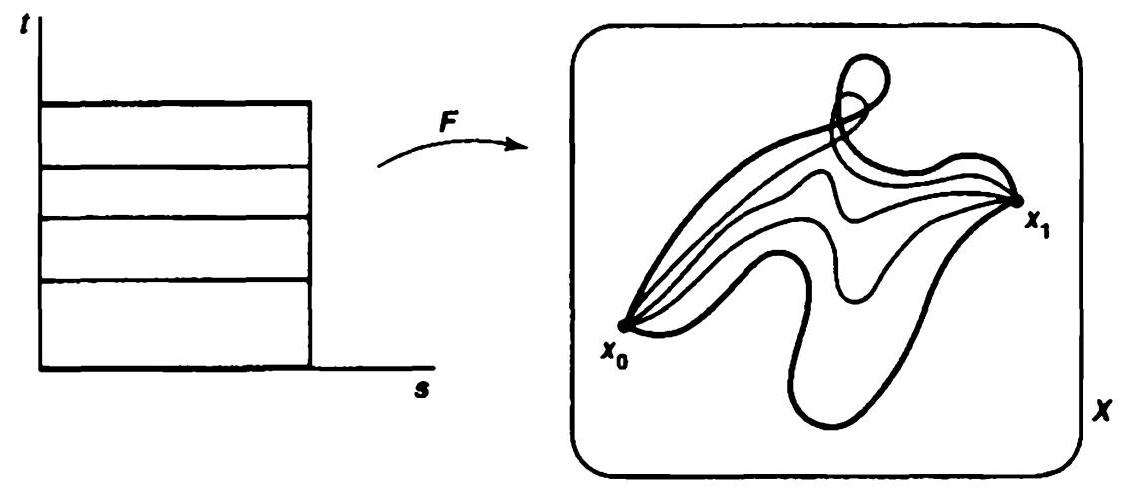
\includegraphics[width=1.0\textwidth]{images/51.1.jpg}
\end{center}
\hspace*{3em} 

Figure 51.1

The first condition says simply that \(F\) is a homotopy between \(f\) and \({f}^{\prime }\) , and the second says that for each \(t\) , the path \({f}_{t}\) defined by the equation \({f}_{t}( s)  = F( {s,t})\) is a path from \({x}_{0}\) to \({x}_{1}\) . Said differently, the first condition says that \(F\) represents a continuous way of deforming the path \(f\) to the path \({f}^{\prime }\) , and the second condition says that the end points of the path remain fixed during the deformation.

\section*{Lemma 51.1. The relations \(\simeq\) and \({ \simeq  }_{p}\) are equivalence relations.}

If \(f\) is a path, we shall denote its path-\index{Homotopy equivalence} class by \([  f]\) .

\begin{proof}
	Let us verify the properties of an equivalence relation.
Given \(f\) , it is trivial that \(f \simeq  f\) ; the map \(F( {x,t})  = f( x)\) is the required homotopy. If \(f\) is a path, \(F\) is a path homotopy.

Given \(f \simeq  {f}^{\prime }\) , we show that \({f}^{\prime } \simeq  f\) . Let \(F\) be a homotopy between \(f\) and \({f}^{\prime }\) . Then \(G( {x,t})  = F( {x,1 - t})\) is a homotopy between \({f}^{\prime }\) and \(f\) . If \(F\) is a path homotopy, so is \(G\) .

Suppose that \(f \simeq  {f}^{\prime }\) and \({f}^{\prime } \simeq  {f}^{\prime \prime }\) . We show that \(f \simeq  {f}^{\prime \prime }\) . Let \(F\) be a homotopy between \(f\) and \({f}^{\prime }\) , and let \({F}^{\prime }\) be a homotopy between \({f}^{\prime }\) and \({f}^{\prime \prime }\) . Define \(G : X \times  I \rightarrow\)  \(\gamma\) by the equation

\[
G( {x,t})  = \{  \begin{array}{ll} F( {x,{2t}}) & \text{ for }t \in  [  {0,\frac{1}{2}}]  , \\  {F}^{\prime }( {x,{2t} - 1}) & \text{ for }t \in  [  {\frac{1}{2},1}]  . \end{array}.
\]

The map \(G\) is well defined, since if \(t = \frac{1}{2}\) , we have \(F( {x,{2t}})  = {f}^{\prime }( x)  = {F}^{\prime }( {x,{2t} - 1})\) . Because \(G\) is continuous on the two closed subsets \(X \times  [  {0,\frac{1}{2}}]\) and \(X \times  [  {\frac{1}{2},1}]\) of \(X \times  I\) , it is continuous on all of \(X \times  I\) , by the pasting lemma. Thus \(G\) is the required homotopy between \(f\) and \({f}^{\prime \prime }\) .

You can check that if \(F\) and \({F}^{\prime }\) are path homotopies, so is \(G\) . See Figure 51.2. is a homotopy between them. It is called a \index{Straight-line homotopy} because it moves the point \(f( x)\) to the point \(g( x)\) along the straight-line segment joining them.

\begin{center}
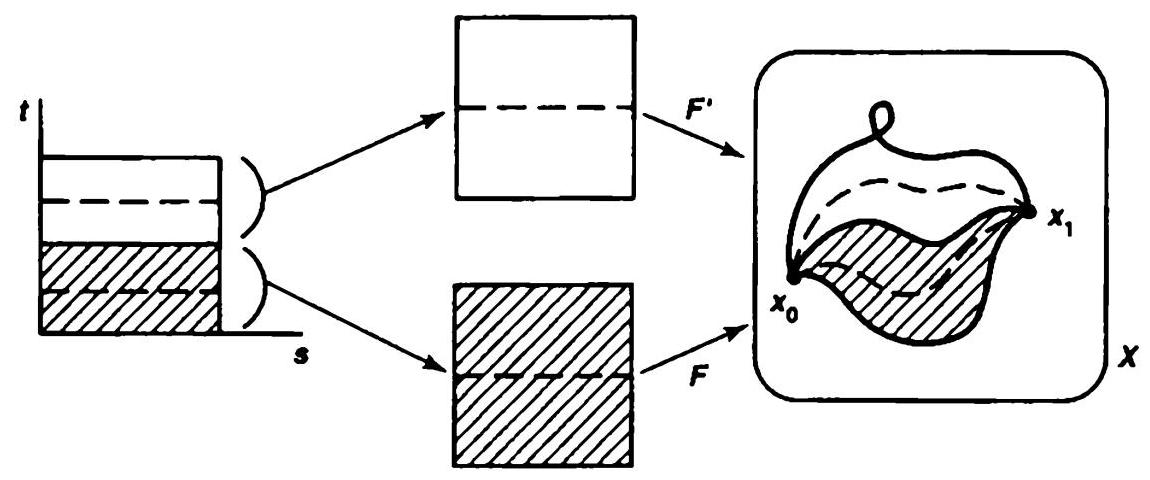
\includegraphics[width=1.0\textwidth]{images/51.2.jpg}
\end{center}
\hspace*{3em} 

Figure 51.2

\begin{centeredblock}
\begin{example}
	Let \(f\) and \(g\) be any two maps of a space \(X\) into \({\mathbb{R}}^{2}\) It is easy to see that \(f\) and \(g\) are homotopic; the map

\[
F( {x,t})  = ( {1 - t}) f( x)  + {tg}( x)
\]

If \(f\) and \(g\) are paths from \({x}_{0}\) to \({x}_{1}\) , then \(F\) will be a path homotopy, as you can check. This situation is pictured in Figure 5.1.3.
\end{example}
\end{centeredblock}

More generally, let \(A\) be any convex subspace of \({\mathbb{R}}^{n}\) . (This means that for any two points \(a,b\) of \(A\) , the straight line segment joining \(a\) and \(b\) is contained in \(A\) .) Then any two paths \(f,g\) in \(A\) from \({x}_{0}\) to \({x}_{1}\) are path homotopic in \(A\) , for the \index{straight-line homotopy@Straight-line homotopy}straight-line homotopy \(F\) between them has image set in \(A\)

\begin{center}
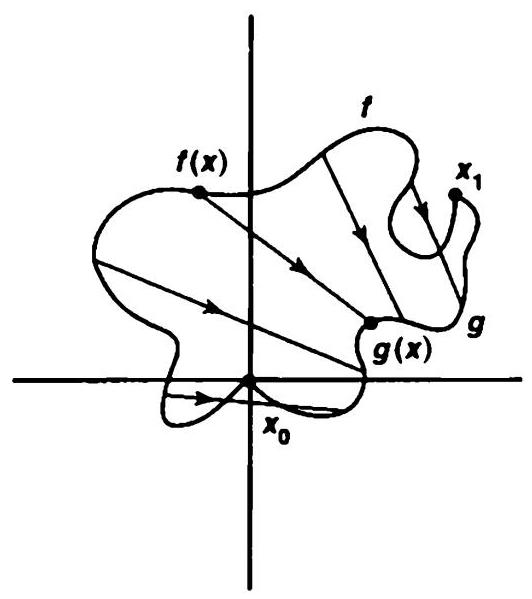
\includegraphics[width=0.4\textwidth]{images/51.3.jpg}
\end{center}
\hspace*{3em} 

Figure 51.3

\begin{center}
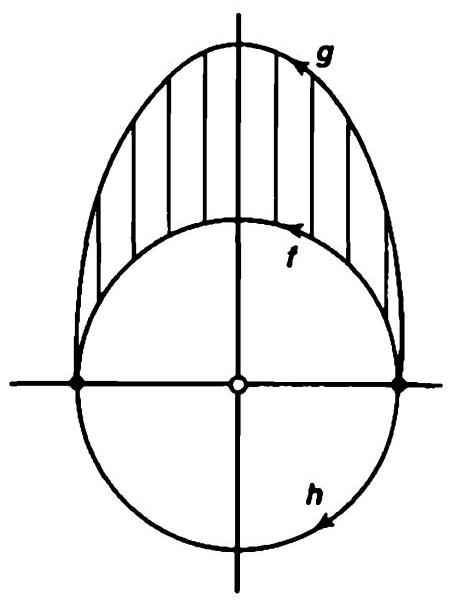
\includegraphics[width=0.4\textwidth]{images/51.4.jpg}
\end{center}
\hspace*{3em} 

Figure 51.4

\begin{centeredblock}
\begin{example}
	Let \(X\) denote the punctured plane, \({\mathbb{R}}^{2} - \{ 0\}\) , which we shall denote by \(\index{R@\({\mathbb{R}}^{2} - 0\)} \index{R@${\mathbb{R}}^{2} - 0$}{\mathbb{R}}^{2} - 0\) for short The following paths in \(X\) ,

\[
f( s)  = ( {\cos {\pi s},\sin {\pi s}}) ,
\]

\[
g( s)  = ( {\cos {\pi s},2\sin {\pi s}})
\]

are path homotopic, the straight-line homotopy between them is an acceptable path homotopy But the straight-line homotopy between \(f\) and the path

\[
h( s)  = ( {\cos {\pi s}, - \sin {\pi s}})
\]

is not acceptable, for its image does not lie in the space \(X = {\mathbb{R}}^{2} - 0\) . See Figure 51.4.

Indeed, there exists no path homotopy in \(X\) between paths \(f\) and \(h\) This result is hardly surprising, it is intuitively clear that one cannot ``deform \(f\) past the hole at 0 `` without introducing a discontinuity. But it takes some work to prove. We shall return to this example later

This example illustrates the fact that you must know what the range space is before you can tell whether two paths are path homotopic or not The paths \(f\) and \(h\) would be path homotopic if they were paths in \({\mathbb{R}}^{2}\)
\end{example}
\end{centeredblock}

Now we introduce some algebra into this geometric situation. We define a certain operation on \index{Path-homotopy class}s as follows:
\end{proof}
\begin{definition}
	If \(f\) is a path in \(X\) from \({x}_{0}\) to \({x}_{1}\) , and if \(g\) is a path in \(X\) from \({x}_{1}\) to \({x}_{2}\) , we define the product \(\index{f@\(f * g\)} \index{f@$f * g$}f * g\) of \(f\) and \(g\) to be the path \(h\) given by the equations

\[
h( s)  = \{  \begin{array}{ll} f( {2s}) & \text{ for }s \in  [  {0,\frac{1}{2}}]  , \\  g( {{2s} - 1}) & \text{ for }s \in  [  {\frac{1}{2},1}]  . \end{array}.
\]

The function \(h\) is well-defined and continuous, by the pasting lemma; it is a path in \(X\) from \({x}_{0}\) to \({x}_{2}\) . We think of \(h\) as the path whose first half is the path \(f\) and whose second half is the path \(g\) .
\end{definition}

The product operation on paths induces a well-defined operation on path-homotopy classes, defined by the equation

\[
[  f]   * [  g]   = [  {f * g}]
\]

To verify this fact, let \(F\) be a path homotopy between \(f\) and \({f}^{\prime }\) and let \(G\) be a path homotopy between \(g\) and \({g}^{\prime }\) . Define

\[
H( {s,t})  = \{  \begin{array}{ll} F( {{2s},t}) & \text{ for }s \in  [  {0,\frac{1}{2}}]  , \\  G( {{2s} - 1,t}) & \text{ for }s \in  [  {\frac{1}{2},1}]  . \end{array}.
\]

Because \(F( {1,t})  = {x}_{1} = G( {0,t})\) for all \(t\) , the map \(H\) is well-defined; it is continuous by the pasting lemma. You can check that \(H\) is the required path homotopy between \(f * g\) and \({f}^{\prime } * {g}^{\prime }\) It is pictured in Figure 51.5.

\begin{center}
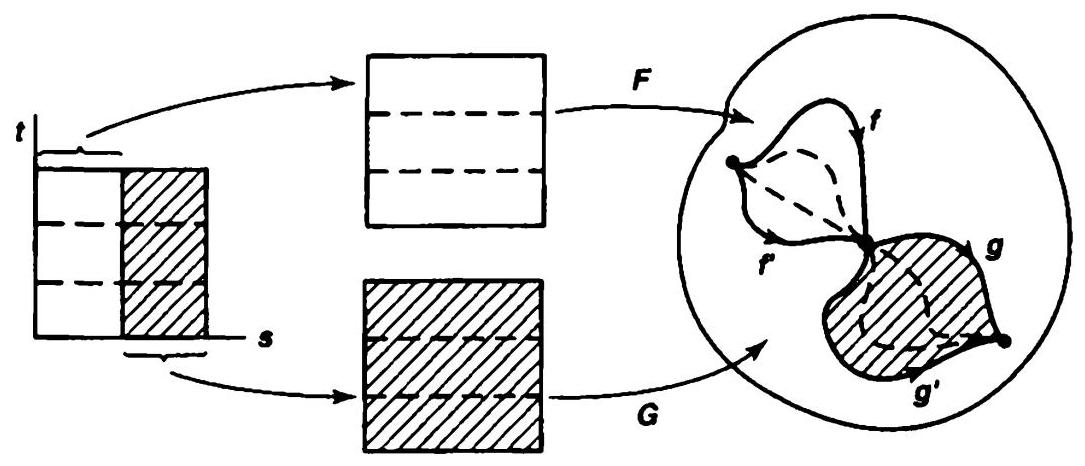
\includegraphics[width=1.0\textwidth]{images/51.5.jpg}
\end{center}
\hspace*{3em} 

Figure 51.5

The operation \(*\) on \index{path-homotopy class@Path-homotopy class}path-homotopy classes turns out to satisfy properties that look very much like the axioms for a group. They are called the \index{Groupoid properties} of \(*\) . One difference from the properties of a group is that \([  f]   * [  g]\) is not defined for every pair of classes, but only for those pairs \([  f]  ,[  g]\) for which \(f( 1)  = g( 0)\) .

\begin{theorem}
	The operation \(*\) has the following properties:

(I) (Associativity) If \([  f]   * ( {[  g]   * [  h]  })\) is defined, so is \(( {[  f]   * [  g]  })  * [  h]\) , and they are equal.

(2) (Right and left identities) Given \(x \in  X\) , let \(\index{e@\({e}_{x}\)} {e}_{x}\) denote the \index{Constant path} \({e}_{x} : I \rightarrow\)  \(X\) carrying all of \(I\) to the point \(x\) . If \(f\) is a path in \(X\) from \({x}_{0}\) to \({x}_{1}\) , then

\[
[  f]   * [  {e}_{{x}_{1}}]   = [  f]  \;\text{ and }\;[  {e}_{{x}_{0}}]   * [  f]   = [  f]  .
\]

(3) (Inverse) Given the path \(f\) in \(X\) from \({x}_{0}\) to \({x}_{1}\) , let \(\bar{f}\) be the path defined by \(\bar{f}( s)  = f( {1 - s})\) . It is called the reverse of \(f\) Then

\[
[  f]   * [  \bar{f}]   = [  {e}_{{x}_{0}}]  \;\text{ and }\;[  \bar{f}]   * [  f]   = [  {e}_{{x}_{1}}]  .
\]
\end{theorem}

\begin{proof}
	We shall make use of two elementary facts. The first is the fact that if \(k\) : \(X \rightarrow  Y\) is a continuous map, and if \(F\) is a path homotopy in \(X\) between the paths \(f\) and \({f}^{\prime }\) , then \(k \circ  F\) is a path homotopy in \(Y\) between the paths \(k \circ  f\) and \(k \circ  {f}^{\prime }\) . See Figure 51.6.
\begin{center}
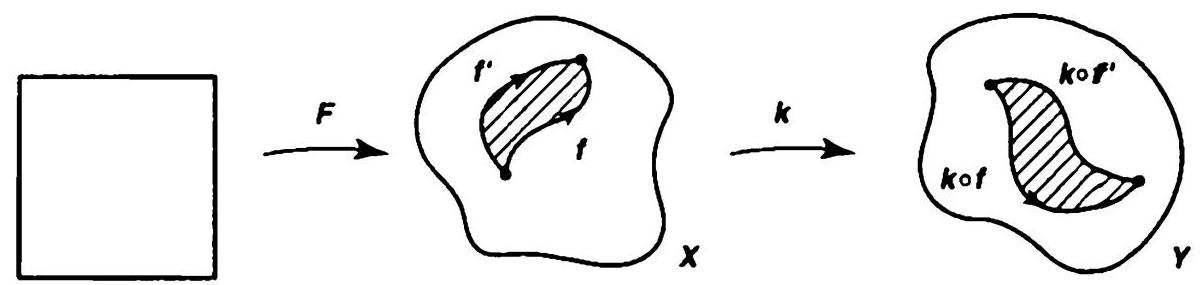
\includegraphics[width=1.0\textwidth]{images/51.6.jpg}
\end{center}
\hspace*{3em} 

Figure 51.6

The second is the fact that if \(k : X \rightarrow  Y\) is a continuous map and if \(f\) and \(g\) are paths in \(X\) with \(f( 1)  = g( 0)\) , then

\[
k \circ  ( {f * g})  = ( {k \circ  f})  * ( {k \circ  g}) .
\]

This equation follows at once from the definition of the product operation \(*\) .

Step 1. We verify properties (2) and (3). To verify (2), we let \({e}_{0}\) denote the \index{constant path@Constant path}constant path in \(I\) at 0, and we let \(i : I \rightarrow  I\) denote the identity map, which is a path in \(I\) from 0 to 1 . Then \({e}_{0} * i\) is also a path in \(I\) from 0 to 1 . (The graphs of these two paths are pictured in Figure 51.7.)

\begin{center}
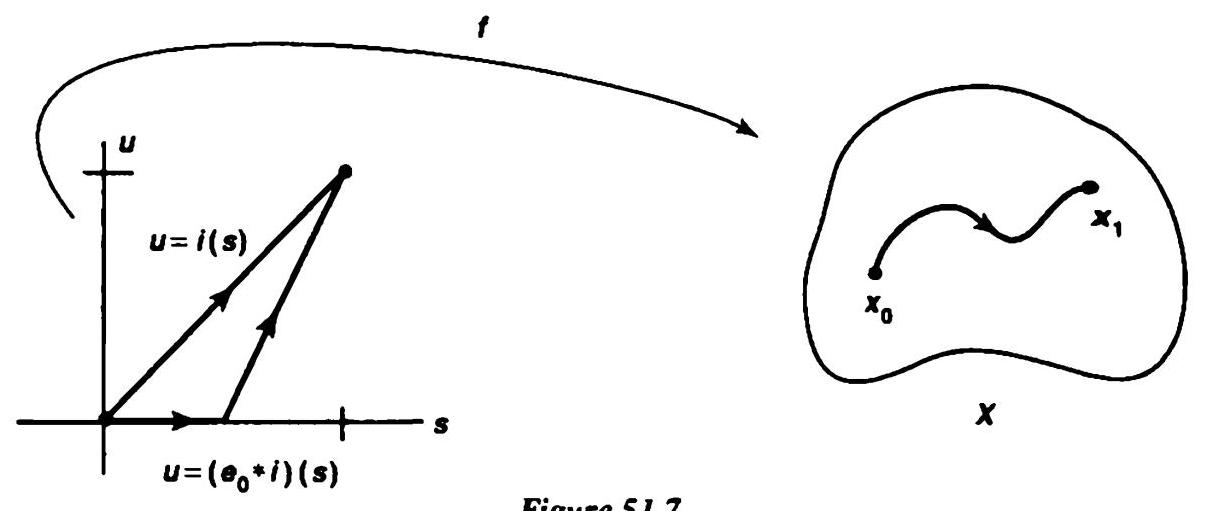
\includegraphics[width=1.0\textwidth]{images/51.7.jpg}
\end{center}
\hspace*{3em} 

Figure 51.7

Because \(I\) is convex, there is a path homotopy \(G\) in \(I\) between \(i\) and \({e}_{0} * i\) . Then \(f \circ  G\) is a path homotopy in \(X\) between the paths \(f \circ  i = f\) and

\[
f \circ  ( {{e}_{0} * i})  = ( {f \circ  {e}_{0}})  * ( {f \circ  i})  = {e}_{{x}_{0}} * f.
\]

An entirely similar argument, using the fact that if \({e}_{1}\) denotes the constant path at 1, then \(i * {e}_{1}\) is path homotopic in \(I\) to the path \(i\) , shows that \([  f]   * [  {e}_{{x}_{1}}]   = [  f]\) .

To verify (3), note that the reverse of \(i\) is \(\bar{i}( s)  = 1 - s\) . Then \(i * \bar{i}\) is a path in \(I\) beginning and ending at 0, and so is the constant path \({e}_{0}\) . (Their graphs are pictured in Figure 51.8.) Because \(I\) is convex, there is a path homotopy \(H\) in \(I\) between \({e}_{0}\) and \(i * \bar{i}\) . Then \(f \circ  H\) is a path homotopy between \(f \circ  {e}_{0} = {e}_{{x}_{0}}\) and

\[
( {f \circ  i})  * ( {f \circ  \bar{i}})  = f * \bar{f}.
\]

An entirely similar argument, using the fact that \(\bar{i} * i\) is path homotopic in \(I\) to \({e}_{1}\) , shows that \([  \bar{f}]   * [  f]   = [  {e}_{{x}_{1}}]\) .

\begin{center}
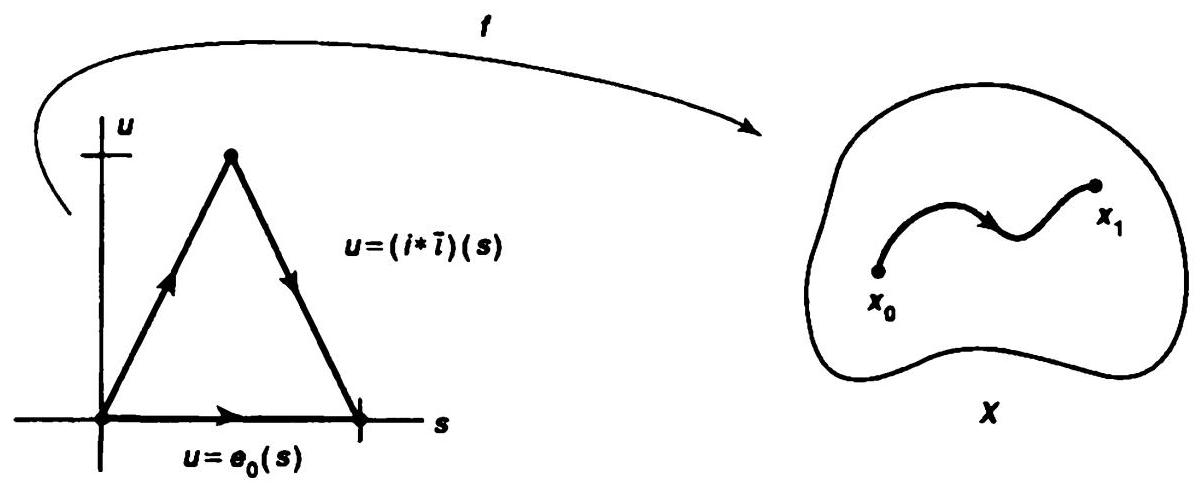
\includegraphics[width=1.0\textwidth]{images/51.8.jpg}
\end{center}
\hspace*{3em} 

Figure 51.8

Step 2. The proof of (1), associativity, is a bit trickier. For this proof, and for later use as well, it will be convenient to describe the product \(f * g\) in a different way.

If \([  {a,b}]\) and \([  {c,d}]\) are two intervals in \(\mathbb{R}\) , there is a unique map \(p : [  {a,b}]   \rightarrow  [  {c,d}]\) of the form \(p( x)  = {mx} + k\) that carries \(a\) to \(c\) and \(b\) to \(d\) ; we call it the \index{positive linear map: of intervals in@Positive linear map: of intervals in} positive linear map of \([  {a,b}]\) to \([  {c,d}]\) because its graph is a straight line with positive slope. Note that the inverse of such a map is another such map, and so is the \index{Covering map!composite}composite of two such maps.

With this terminology, the product \(f * g\) can be described as follows: \(\operatorname{On}[  {0,\frac{1}{2}}]\) , it equals the positive linear map of \([  {0,\frac{1}{2}}]\) to \([  {0,1}]\) , followed by \(f\) ; and on \([  {\frac{1}{2},1}]\) , it equals the positive linear map of \([  {\frac{1}{2},1}]\) to \([  {0,1}]\) , followed by \(g\) .

Now we verify (1). Given paths \(f,g\) , and \(h\) in \(X\) , the products \(f * ( {g * h})\) and \(( {f * g})  * h\) are defined precisely when \(f( 1)  = g( 0)\) and \(g( 1)  = h( 0)\) . Assuming these two conditions, we define also a ``triple product'' of the paths \(f,g\) , and \(h\) as follows: Choose points \(a\) and \(b\) of \(I\) so that \(0 < a < b < 1\) . Define a path \({k}_{a,b}\) in \(X\) as follows: On \([  {0,a}]\) it equals the positive linear map of \([  {0,a}]\) to \(I\) followed by \(f\) ; on \([  {a,b}]\) it equals the positive linear map of \([  {a,b}]\) to \(l\) followed by \(g\) ; and on \([  {b,1}]\) it equals the positive linear map of \([  {b,1}]\) to \(l\) followed by \(h\) . The path \({k}_{a,b}\) depends of course on the choice of the points \(a\) and \(b\) . But its path-homotopy class does not! We show that if \(c\) and \(d\) are another pair of points of \(I\) with \(0 < c < d < 1\) , then \({k}_{c,d}\) is path homotopic to \({k}_{a,b}\) .

Let \(p : I \rightarrow  I\) be the map whose graph is pictured in Figure 519. When restricted to \([  {0,a}]  ,[  {a,b}]\) , and \([  {b,1}]\) , respectively, it equals the positive linear maps of these intervals onto \([  {0,c}]  ,[  {c,d}]\) , and \([  {d,1}]\) , respectively. It follows at once that \({k}_{c,d} \circ  p\) equals \({k}_{a,b}\) . But \(p\) is a path in \(I\) from 0 to 1 ; and so is the identity map \(i : I \rightarrow  I\) . Hence, there is a path homotopy \(P\) in \(I\) between \(p\) and \(i\) . Then \({k}_{c,d} \circ  P\) is a path homotopy in \(X\) between \({k}_{a,b}\) and \({k}_{c,d}\)

\begin{center}
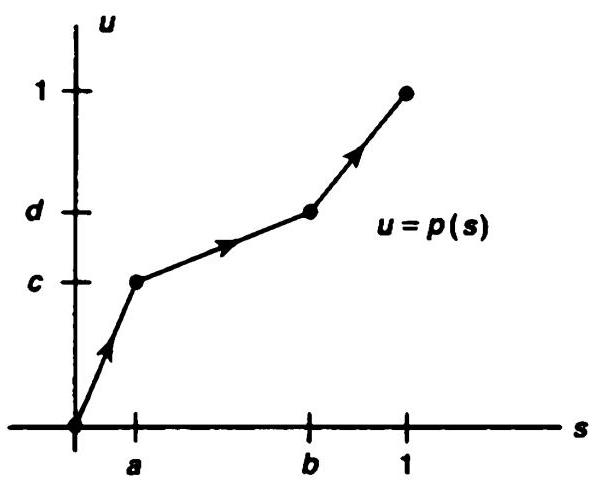
\includegraphics[width=0.5\textwidth]{images/51.9.jpg}
\end{center}
\hspace*{3em} 

Figure 51.9

What has this to do with associativity? A great deal. For the product \(f * ( {g * h})\) is exactly the triple product \({k}_{a,b}\) in the case where \(a = 1/2\) and \(b = 3/4\) , as you can check, while the product \(( {f * g})  * h\) equals \({k}_{c,d}\) in the case where \(c = 1/4\) and \(d = 1/2\) . Therefore these two products are path homotopic.

The argument just used to prove associativity goes through for any finite product \index{Product: of continuous maps!of paths}of paths. Roughly speaking, it says that as far as the path-homotopy class of the result is concerned, it doesn't matter how you chop up the interval when you form the product of paths! This result will be useful to us later, so we state it formally as a theorem here:
\end{proof}
\begin{theorem}
	Let \(f\) be a path in \(X\) , and let \({a}_{0},\ldots ,{a}_{n}\) be numbers such that \(0 = {a}_{0} < {a}_{1} < \cdots  < {a}_{n} = 1\) . Let \({f}_{i} : I \rightarrow  X\) be the path that equals the positive linear map of \(I\) onto \([  {{a}_{i - 1},{a}_{i}}]\) followed by \(f\) . Then

\[
[  f]   = [  {f}_{1}]   * \cdots  * [  {f}_{n}]  .
\]
\end{theorem}

\section*{Exercises}
\begin{enumerate}[itemsep=0.4em, parsep=0pt, topsep=0pt, partopsep=0pt, leftmargin=*, label=\arabic*., ref=\arabic*]
\item Show that if \(h,{h}^{\prime } : X \rightarrow  Y\) are homotopic and \(k,{k}^{\prime } : Y \rightarrow  Z\) are homotopic, then \(k \circ  h\) and \({k}^{\prime } \circ  {h}^{\prime }\) are homotopic.
\item Given spaces \(X\) and \(Y\) , let \(\index{X@\([  {X,Y}]\)}\) denote the set of homotopy classes of maps of \(X\) into \(Y\) .
  \begin{enumerate}[itemsep=0.2em, parsep=0pt, topsep=0pt, partopsep=0pt, leftmargin=*, label=(\alph*), align=left]
  \item Let \(I = [  {0,1}]\) . Show that for any \(X\) , the set \([  {X,I}]\) has a single element.
  \item Show that if \(Y\) is path connected, the set \([  {I,Y}]\) has a single element.
  \end{enumerate}
\item A space \(X\) is said to be contractible if the identity map \({i}_{X} : X \rightarrow  X\) is nulho-motopic.
  \begin{enumerate}[itemsep=0.2em, parsep=0pt, topsep=0pt, partopsep=0pt, leftmargin=*, label=(\alph*), align=left]
  \item Show that \(I\) and \(\mathbb{R}\) are contractible.
  \item Show that a \index{Contractible space} is path connected.
  \item Show that if \(Y\) is contractible, then for any \(X\) , the set \([  {X,Y}]\) has a single element.
  \item Show that if \(X\) is contractible and \(Y\) is path connected, then \([  {X,Y}]\) has a single element.
  \end{enumerate}
\end{enumerate}
\section*{§ 52 The Fundamental Group}

The set of path-homotopy classes of paths in a space \(X\) does not form a group under the operation \(*\) because the product of two path-homotopy classes is not always defined. But suppose we pick out a point \({x}_{0}\) of \(X\) to serve as a \index{Base point!effect on \({\pi }_{1}\)} ``\index{Base point}'' and restrict ourselves to those paths that begin and end at \({x}_{0}\) The set of these path-homotopy classes does form a group under \(*\) . It will be called the fundamental group of \(X\) .

In this section, we shall study the fundamental group and derive some of its properties. In particular, we shall show that the group is a topological invariant of the space \(X\) , the fact that is of crucial importance in using it to study homeomorphism problems.

Let us first review some terminology from group theory. Suppose \(G\) and \({G}^{\prime }\) are groups, written multiplicatively A \index{path-induced homomorphism@Path-induced homomorphism} homomorphism \(f : G \rightarrow  {G}^{\prime }\) is a map such that \(f( {x \cdot  y})  = f( x)  \cdot  f( y)\) for all \(x,y\) ; it automatically satisfies the equations \(f( e)  = {e}^{\prime }\) and \(f( {x}^{-1})  = f{( x) }^{-1}\) , where \(e\) and \({e}^{\prime }\) are the identities of \(G\) and \({G}^{\prime }\) , respectively, and the exponent -1 denotes the inverse. The \index{kernel of homomorphism@Kernel of homomorphism} kernel of \(f\) is the set \({f}^{-1}( {e}^{\prime })\) ; it is a subgroup of \(G\) . The image of \(f\) , similarly, is a subgroup of \({G}^{\prime }\) . The \index{homomorphism@Homomorphism}homomorphism \(f\) is called a \index{Monomorphism} if it is injective (or equivalently, if the kernel of \(f\) consists of \(e\) alone). It is called an \index{Epimorphism} if it is surjective; and it is called an isomorphism if it is bijective

Suppose \(G\) is a group and \(H\) is a subgroup of \(G\) . Let \({xH}\) denote the set of all products \({xh}\) , for \(h \in  H\) ; it is called a left coset of \(H\) in \(G\) . The collection of all such cosets forms a partition of \(G\) . Similarly, the collection of all \index{Right coset} \({Hx}\) of \(H\) in \(G\) forms a partition of \(G\) . We call \(H\) a \index{Normal subgroup} of \(G\) if \(x \cdot  h \cdot  {x}^{-1} \in  H\) for each \(x \in  G\) and each \(h \in  H\) . In this case, we have \({xH} = {Hx}\) for each \(x\) , so that our two partitions of \(G\) are the same. We denote this partition by \(G/H\) ; if one defines

\[
( {xH})  \cdot  ( {yH})  = ( {x \cdot  y}) H
\]

one obtains a well-defined operation on \(G/H\) that makes it a group. This group is called the quotient of \(G\) by \(H\) . The map \(f : G \rightarrow  G/H\) carrying \(x\) to \({xH}\) is an \index{epimorphism@Epimorphism}epimorphism with kernel \(H\) Conversely, if \(f : G \rightarrow  {G}^{\prime }\) is an epimorphism, then its kernel \(N\) is a \index{normal subgroup@Normal subgroup}normal subgroup of \(G\) , and \(f\) induces an isomorphism \(G/N \rightarrow  {G}^{\prime }\) that carries \({xN}\) to \(f( x)\) for each \(x \in  G\) .

If the subgroup \(H\) of \(G\) is not normal, it will still be convenient to use the symbol \(G/H\) ; we will use it to denote the collection of \index{right coset@Right coset}right cosets of \(H\) in \(G\) .

Now we define the fundamental group.

\begin{definition}
	Let \(X\) be a space; let \({x}_{0}\) be a point of \(X\) . A path in \(X\) that begins and ends at \({x}_{0}\) is called a \index{Loop} based at \({x}_{0}\) . The set of path homotopy classes of \index{loop@Loop}loops based at \({x}_{0}\) , with the operation \(*\) , is called the fundamental group of \(X\) relative to the \index{base point@Base point}base point \({x}_{0}\) . It is denoted by \(\index{pi@\({\pi }_{1}( {X,{x}_{0}})\)} {\pi }_{1}( {X,{x}_{0}})\) .
\end{definition}

It follows from Theorem 51.2 that the operation \(*\) , when restricted to this set, satisfies the axioms for a group. Given two loops \(f\) and \(g\) based at \({x}_{0}\) , the product \(f * g\) is always defined and is a loop based at \({x}_{0}\) . Associativity, the existence of an identity element \([  {e}_{{x}_{0}}]\) , and the existence of an inverse \([  \bar{f}]\) for \([  f]\) are immediate.

Sometimes this group is called the first homotopy group of \(X\) , which term implies that there is a second homotopy group. There are indeed groups \({\pi }_{n}( {X,{x}_{0}})\) for all \(n \in  {\mathbb{Z}}_{ + }\) , but we shall not study them in this book. They are part of the general subject called homotopy theory.

\begin{centeredblock}
\begin{example}
	Let \({\mathbb{R}}^{n}\) denote euclidean \(n\) -space. Then \({\pi }_{1}( {{\mathbb{R}}^{n},{x}_{0}})\) is the trivial group (the group consisting of the identity alone). For if \(f\) is a loop in \({\mathbb{R}}^{n}\) based at \({x}_{0}\) , the straight-line homotopy is a path homotopy between \(f\) and the constant path at \({x}_{0}\) . More generally, if \(X\) is any convex subset of \({\mathbb{R}}^{n}\) , then \({\pi }_{1}( {X,{x}_{0}})\) is the trivial group. In particular, the unit ball \({B}^{n}\) in \({\mathbb{R}}^{n}\) .

\[
{B}^{n} = \{  {\mathbf{x} \mid  {x}_{1}^{2} + \; + {x}_{n}^{2} \leq  1}\}  ,
\]

has trivial fundamental group.
\end{example}
\end{centeredblock}

An immediate question one asks is the extent to which the fundamental group depends on the base point. We consider that question now.

\begin{definition}
	Let \(\alpha\) be a path in \(X\) from \({x}_{0}\) to \({x}_{1}\) . We define a map

\[
\widehat{\alpha } : {\pi }_{1}( {X,{x}_{0}})  \rightarrow  {\pi }_{1}( {X,{x}_{1}})
\]

by the equation

\[
\widehat{\alpha }( [  f]  )  = [  \bar{\alpha }]   * [  f]   * [  \alpha ]  .
\]

The map \(\widehat{\alpha }\) , which we call `` \(\alpha\) -hat,'' is well-defined because the operation \(*\) is well-defined. If \(f\) is a loop based at \({x}_{0}\) , then \(\bar{\alpha } * ( {f * \alpha })\) is a loop based at \({x}_{1}\) . Hence \(\widehat{\alpha }\) maps \({\pi }_{1}( {X,{x}_{0}})\) into \({\pi }_{1}( {X,{x}_{1}})\) , as desired; note that it depends only on the path-homotopy class of \(\alpha\) . It is pictured in Figure 521.
\end{definition}

\begin{center}
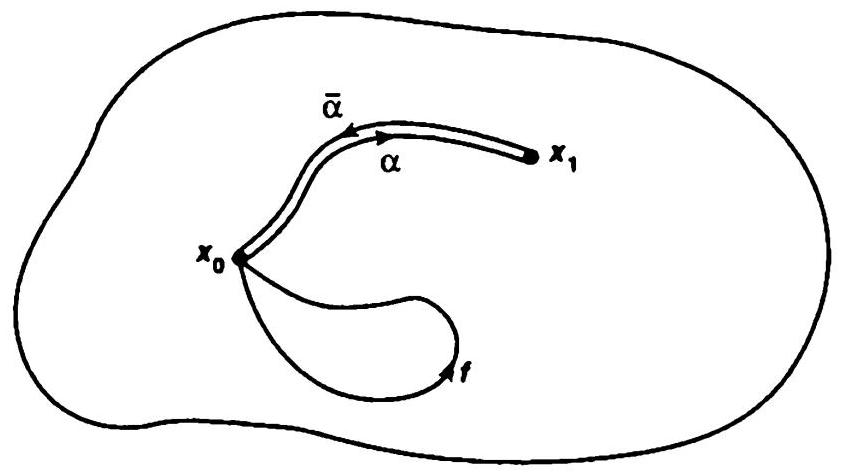
\includegraphics[width=0.7\textwidth]{images/52.1.jpg}
\end{center}
\hspace*{3em} 

Figure 52.1

\begin{theorem}
	The map \(\widehat{\alpha }\) is a group isomorphism.
\end{theorem}

\begin{proof}
	To show that \(\widehat{\alpha }\) is a homomorphism, we compute
\[
\widehat{\alpha }( [  f]  )  * \widehat{\alpha }( [  g]  )  = ( {[  \bar{\alpha }]   * [  f]   * [  \alpha ]  })  * ( {[  \bar{\alpha }]   * [  g]   * [  \alpha ]  })
\]

\[
= [  \bar{\alpha }]   * [  f]   * [  g]   * [  \alpha ]
\]

\[
= \widehat{\alpha }( {[  f]   * [  g]  }) \text{ . }
\]

To show that \(\widehat{\alpha }\) \index{alpha@\widehat{\alpha}!is an isomorphism}is an isomorphism, we show that if \(\beta\) denotes the path \(\bar{\alpha }\) , which is the reverse of \(\alpha\) , then \(\widehat{\beta }\) is an inverse for \(\widehat{\alpha }\) . We compute, for each element \([  h]\) of \({\pi }_{1}( {X,{x}_{1}})\) ,

\[
\widehat{\beta }( [  h]  )  = [  \bar{\beta }]   * [  h]   * [  \beta ]   = [  \alpha ]   * [  h]   * [  \bar{\alpha }]  ,
\]

\[
\widehat{\alpha }( {\widehat{\beta }( [  h]  ) })  = [  \bar{\alpha }]   * ( {[  \alpha ]   * [  h]   * [  \bar{\alpha }]  })  * [  \alpha ]   = [  h]  .
\]

A similar computation shows that \(\widehat{\beta }( {\widehat{\alpha }( [  f]  ) })  = [  f]\) for each \([  f]   \in  {\pi }_{1}( {X,{x}_{0}})\) .
\end{proof}
\begin{corollary}
	If \(X\) is path connected and \({x}_{0}\) and \({x}_{1}\) are two points of \(X\) , then \({\pi }_{1}( {X,{x}_{0}})\) is isomorphic to \({\pi }_{1}( {X,{x}_{1}})\) .
\end{corollary}

Suppose that \(X\) is a topological space. Let \(C\) be the path component of \(X\) containing \({x}_{0}\) It is easy to see that \({\pi }_{1}( {C,{x}_{0}})  = {\pi }_{1}( {X,{x}_{0}})\) , since all loops and homotopies in \(X\) that are based at \({x}_{0}\) must lie in the subspace \(C\) . Thus \({\pi }_{1}( {X,{x}_{0}})\) depends on only the path component of \(X\) containing \({x}_{0}\) ; it gives us no information whatever about the rest of \(X\) . For this reason, it is usual to deal with only path-connected spaces when studying the fundamental group

If \(X\) is path connected, all the groups \({\pi }_{1}( {X,x})\) are isomorphic, so it is tempting to try to ``identify'' all these groups with one another and to speak simply of the fundamental group of the space \(X\) , without reference to base point. The difficulty with this approach is that there is no natural way of identifying \({\pi }_{1}( {X,{x}_{0}})\) with \({\pi }_{1}( {X,{x}_{1}})\) ; different paths \(\alpha\) and \(\beta\) from \({x}_{0}\) to \({x}_{1}\) may give rise to different isomorphisms between these groups. For this reason, omitting the base point can lead to error.

It turns out that the isomorphism of \({\pi }_{1}( {X,{x}_{0}})\) with \({\pi }_{1}( {X,{x}_{1}})\) \index{alpha@\widehat{\alpha}!independent of path}is independent of path if and only if the fundamental group is abelian. (See Exercise 3.) This is a stringent requirement on the space \(X\) .

\begin{definition}
	A space \(X\) is said to be simply connected if it is a path-connected space and if \({\pi }_{1}( {X,{x}_{0}})\) is the trivial (one-element) group for some \({x}_{0} \in  X\) , and hence for every \({x}_{0} \in  X\) . We often express the fact that \({\pi }_{1}( {X,{x}_{0}})\) is the trivial group by writing \({\pi }_{1}( {X,{x}_{0}})  = 0.\)
\end{definition}

\begin{lemma}
	In a simply connected space \(X\) , any two paths having the same initial and final points are path homotopic.
\end{lemma}

\begin{proof}
	Let \(\alpha\) and \(\beta\) be two paths from \({x}_{0}\) to \({x}_{1}\) Then \(\alpha  * \bar{\beta }\) is defined and is a loop on \(X\) based at \({x}_{0}\) . Since \(X\) is simply connected, this loop is path homotopic to the constant loop at \({x}_{0}\) . Then
\[
[  {\alpha  * \bar{\beta }}]   * [  \dot{\beta }]   = [  {e}_{{x}_{0}}]   * [  \beta ]  ,
\]

from which it follows that \([  \alpha ]   = [  \beta ]\) .

It is intuitively clear that the fundamental group is a topological invariant of the space \(X\) . A convenient way to prove this fact formally is to introduce the notion of the ``homomorphism induced by a continuous map.''

Suppose that \(h : X \rightarrow  Y\) is a continuous map that carries the point \({x}_{0}\) of \(X\) to the point \({y}_{0}\) of \(Y\) . We often denote this fact by writing

\[
h : ( {X,{x}_{0}})  \rightarrow  ( {Y,{y}_{0}}) .
\]

If \(f\) is a loop in \(X\) based at \({x}_{0}\) , then the composite \(h \circ  f : I \rightarrow  Y\) is a loop in \(Y\) based at \({y}_{0}\) . The correspondence \(f \rightarrow  h \circ  f\) thus gives rise to a map carrying \({\pi }_{1}( {X,{x}_{0}})\) into \({\pi }_{1}( {Y,{y}_{0}})\) . We define it formally as follows:
\end{proof}
\begin{definition}
	Let \(h.( {X,{x}_{0}})  \rightarrow  ( {Y,{y}_{0}})\) be a continuous map. Define

\[
\index{h@\({h}_{ * }\)} {h}_{ * }.{\pi }_{1}( {X,{x}_{0}})  \rightarrow  {\pi }_{1}( {Y,{y}_{0}})
\]

by the equation

\[
{h}_{ * }( [  f]  )  = [  {h \circ  f}]  \text{ . }
\]

The map \({h}_{ * }\) is called the homomorphism induced by \(h\) , relative to the base point \({x}_{0}\) .
\end{definition}

The map \({h}_{ * }\) is well-defined, for if \(F\) is a path homotopy between the paths \(f\) and \({f}^{\prime }\) , then \(h \circ  F\) is a path homotopy between the paths \(h \circ  f\) and \(h \circ  {f}^{\prime }\) . The fact that \({h}_{ * }\) is a homomorphism follows from the equation

\[
( {h \circ  f})  * ( {h \circ  g})  = h \circ  ( {f * g}) .
\]

The homomorphism \({h}_{ * }\) depends not only on the map \(h : X \rightarrow  Y\) but also on the choice of the base point \({x}_{0}\) . (Once \({x}_{0}\) is chosen, \({y}_{0}\) is determined by \(h\) .) So some notational difficulty will arise if we want to consider several different base points for \(X\) . If \({x}_{0}\) and \({x}_{1}\) are two different points of \(X\) , we cannot use the same symbol \({h}_{ * }\) to stand for two different homomorphisms, one having domain \({\pi }_{1}( {X,{x}_{0}})\) and the other having domain \({\pi }_{1}( {X,{x}_{1}})\) . Even if \(X\) is path connected, so these groups are isomorphic, they are still not the same group. In such a case, we shall use the notation

\[
{( {h}_{{x}_{0}}) }_{ * } : {\pi }_{1}( {X,{x}_{0}})  \rightarrow  {\pi }_{1}( {Y,{y}_{0}})
\]

for the first homomorphism and \({( {h}_{{x}_{1}}) }_{ * }\) for the second. If there is only one \index{Base point!effect on \({h}_{ * }\)}base point under consideration, we shall omit mention of the base point and denote the induced homomorphism merely by \({h}_{ * }\) .

The induced homomorphism has two properties that are crucial in the applications. They are called its ``\index{\({h}_{ * }\)!functorial properties}functorial properties'' and are given in the following theorem:

\begin{theorem}
	If \(h : ( {X,{x}_{0}})  \rightarrow  ( {Y,{y}_{0}})\) and \(k : ( {Y,{y}_{0}})  \rightarrow  ( {Z,{z}_{0}})\) are continuous, then \({( k \circ  h) }_{ * } = {k}_{ * } \circ  {h}_{ * }\) If \(i : ( {X,{x}_{0}})  \rightarrow  ( {X,{x}_{0}})\) is the identity map, then \({i}_{ * }\) is the identity homomorphism.
\end{theorem}

\begin{proof}
	The proof is a triviality. By definition,
\[
{( k \circ  h) }_{ * }( [  f]  )  = [  {( {k \circ  h})  \circ  f}]  ,
\]

\[
( {{k}_{ * } \circ  {h}_{ * }}) ( [  f]  )  = {k}_{ * }( {{h}_{ * }( [  f]  ) })  = {k}_{ * }( [  {h \circ  f}]  )  = [  {k \circ  ( {h \circ  f}) }]  .
\]

Similarly, \({i}_{ * }( [  f]  )  = [  {i \circ  f}]   = [  f]\)
\end{proof}
\begin{corollary}
	If \(h : ( {X,{x}_{0}})  \rightarrow  ( {Y,{y}_{0}})\) is a homeomorphism of \(X\) with \(Y\) , then \({h}_{ * }\) is an isomorphism of \({\pi }_{1}( {X,{x}_{0}})\) with \({\pi }_{1}( {Y,{y}_{0}})\) .
\end{corollary}

\begin{proof}
	Let \(k \cdot  ( {Y,{y}_{0}})  \rightarrow  ( {X,{x}_{0}})\) be the inverse of \(h\) . Then \({k}_{ * } \circ  {h}_{ * } = {( k \circ  h) }_{ * } = {i}_{ * }\) , where \(i\) is the identity map of \(( {X,{x}_{0}})\) ; and \({h}_{ * } \circ  {k}_{ * } = {( h \circ  k) }_{ * } = {j}_{ * }\) , where \(j\) is the identity map of \(( {Y,{y}_{0}})\) . Since \({i}_{ * }\) and \({j}_{ * }\) are the identity homomorphisms of the groups \({\pi }_{1}( {X,{x}_{0}})\) and \({\pi }_{1}( {Y,{y}_{0}})\) , respectively, \({k}_{ * }\) is the inverse of \({h}_{ * }\) .
\end{proof}
\section*{Exercises}
\begin{enumerate}[itemsep=0.4em, parsep=0pt, topsep=0pt, partopsep=0pt, leftmargin=*, label=\arabic*., ref=\arabic*]
\item A subset \(A\) of \({\mathbb{R}}^{n}\) is said to be \index{star-convex set@Star-convex set} star convex if for some point \({a}_{0}\) of \(A\) , all the line segments joining \({a}_{0}\) to other points of \(A\) lie in \(A\) .
  \begin{enumerate}[itemsep=0.2em, parsep=0pt, topsep=0pt, partopsep=0pt, leftmargin=*, label=(\alph*), align=left]
  \item Find a star convex set that is not convex.
  \item Show that if \(A\) is star convex, \(A\) is simply connected.
  \end{enumerate}
\item Let \(\alpha\) be a path in \(X\) from \({x}_{0}\) to \({x}_{1}\) ; let \(\beta\) be a path in \(X\) from \({x}_{1}\) to \({x}_{2}\) . Show that if \(\gamma  = \alpha  * \beta\) , then \(\widehat{\gamma } = \widehat{\beta } \circ  \widehat{\alpha }\) .
\item Let \({x}_{0}\) and \({x}_{1}\) be points of the path-connected space \(X\) . Show that \({\pi }_{1}( {X,{x}_{0}})\) is abelian if and only if for every pair \(\alpha\) and \(\beta\) of paths from \({x}_{0}\) to \({x}_{1}\) , we have \(\widehat{\alpha } = \widehat{\beta }\) .
\item Let \(A \subset  X\) ; suppose \(r : X \rightarrow  A\) is a continuous map such that \(r( a)  = a\) for each \(a \in  A\) . (The map \(r\) is called a \index{Retraction} of \(X\) onto \(A\) ) If \({a}_{0} \in  A\) , show that \[ {r}_{ * } : {\pi }_{1}( {X,{a}_{0}})  \rightarrow  {\pi }_{1}( {A,{a}_{0}}) \] is surjective.
\item Let \(A\) be a subspace of \({\mathbb{R}}^{n}\) ; let \(h : ( {A,{a}_{0}})  \rightarrow  ( {Y,{y}_{0}})\) . Show that if \(h\) is extendable to a continuous map of \({\mathbb{R}}^{n}\) into \(Y\) , then \({h}_{ * }\) is the \index{Trivial homomorphism} (the homomorphism that maps everything to the identity element).
\item Show that if \(X\) is path connected, the homomorphism induced by a continuous map is independent of base point, up to isomorphisms of the groups involved. More precisely, let \(h : X \rightarrow  Y\) be continuous, with \(h( {x}_{0})  = {y}_{0}\) and \(h( {x}_{1})  = {y}_{1}\) . Let \(\alpha\) be a path in \(X\) from \({x}_{0}\) to \({x}_{1}\) , and let \(\beta  = h \circ  \alpha\) . Show that \[ \widehat{\beta } \circ  {( {h}_{{x}_{0}}) }_{ * } = {( {h}_{{x}_{1}}) }_{ * } \circ  \widehat{\alpha }. \] This equation expresses the fact that the following diagram of maps ``commutes.'' \begin{center} 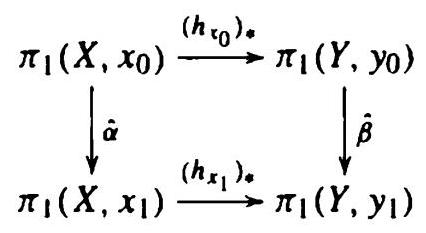
\includegraphics[width=0.3\textwidth]{images/52.2.jpg} \end{center} \hspace*{3em}
\item Let \(G\) be a topological group with operation - and identity element \({x}_{0}\) Let \(\Omega ( {G,{x}_{0}})\) denote the set of all loops in \(G\) based at \({x}_{0}\) . If \(f,g \in  \Omega ( {G,{x}_{0}})\) , let us define a loop \(f \otimes  g\) by the rule \[ ( {f \otimes  g}) ( s)  = f( s)  \cdot  g( s) . \]
  \begin{enumerate}[itemsep=0.2em, parsep=0pt, topsep=0pt, partopsep=0pt, leftmargin=*, label=(\alph*), align=left]
  \item Show that this operation makes the set \(\Omega ( {G,{x}_{0}})\) into a group.
  \item Show that this operation induces a group operation \(\otimes\) on \({\pi }_{1}( {G,{x}_{0}})\) .
  \item Show that the two group operations \(*\) and \(\otimes\) on \({\pi }_{1}( {G,{x}_{0}})\) are the same. [Hint: Compute \(( {f * {e}_{{x}_{0}}})  \otimes  ( {{e}_{{x}_{0}} * g})\) ]
  \item Show that \({\pi }_{1}( {G,{x}_{0}})\) is abelian.
  \end{enumerate}
\end{enumerate}
\section*{§ 53 Covering Spaces}

\index{covering space@Covering Space} We have shown that any convex subspace of \({\mathbb{R}}^{n}\) has a trivial fundamental group; we turn now to the task of computing some fundamental groups that are not trivial. One of the most useful tools for this purpose is the notion of \index{covering space@Covering space}covering space, which we introduce in this section. \index{\({S}^{1}\)!covering spaces}Covering spaces are also important in the study of Riemann surfaces and complex \index{prüfer manifold@Prüfer manifold} manifolds. (See 		\cite{AhlforsSario1960}.) We shall study them in more detail in Chapter 13. Definition. Let \(p\;E \rightarrow  B\) be a continuous surjective map. The open set \(U\) of \(B\) is said to be \index{Evenly covered} by \(p\) if the inverse image \({p}^{-1}( U)\) can be written as the union of disjoint open sets \({V}_{\alpha }\) in \(E\) such that for each \(\alpha\) , the \index{restriction: of a covering map@Restriction: of a covering map} restriction of \(p\) to \({V}_{\alpha }\) is a homeomorphism of \({V}_{\alpha }\) onto \(U\) The collection \(\{  {V}_{\alpha }\}\) will be called a partition of \({p}^{-1}( U)\) into \index{slice: in covering space@Slice: in covering space} slices

If \(U\) is an open set that is evenly covered by \(p\) , we often picture the set \({p}^{-1}( U)\) as a ``stack of pancakes,'' each having the same size and shape as \(U\) , floating in the arr above \(U\) ; the map \(p\) squashes them all down onto \(U\) . See Figure 53.1. Note that if \(U\) is \index{evenly covered@Evenly covered}evenly covered by \(p\) and \(W\) is an open set contained in \(U\) , then \(W\) is also evenly covered by \(p\) .

\begin{center}
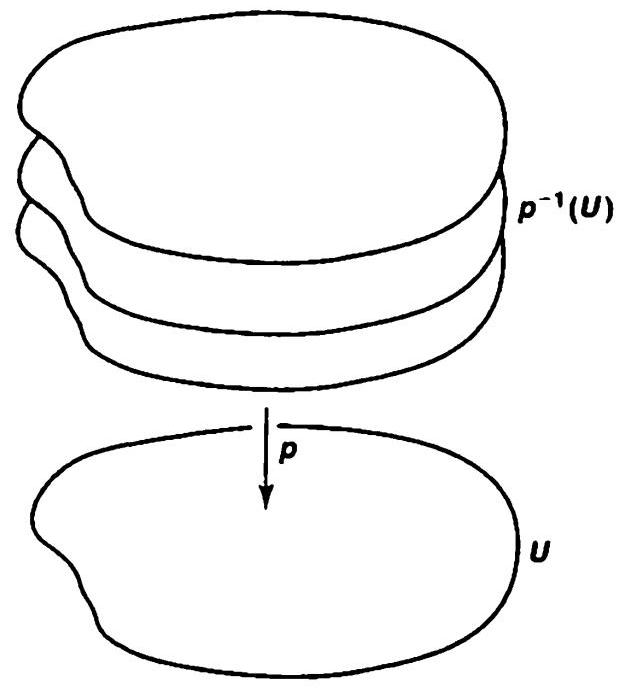
\includegraphics[width=0.5\textwidth]{images/53.1.jpg}
\end{center}
\hspace*{3em} 

Figure 53.1

\begin{definition}
	Let \(p : B \rightarrow  B\) be continuous and surjective. If every point \(b\) of \(B\) has a neighborhood \(U\) that is evenly covered by \(p\) , then \(p\) is called a \index{Covering map}, and \(E\) is said to be a covering space of \(B\)
\end{definition}

Note that if \(p : E \rightarrow  B\) is a covering map, then for each \(b \in  B\) the subspace \({p}^{-1}( b)\) of \(E\) has the discrete topology For each slice \({V}_{\alpha }\) \index{Covering map!is open}is open in \(E\) and intersects the set \({p}^{-1}( b)\) in a single point; therefore, this point is open in \({p}^{-1}( b)\) .

Note also that if \(p : E \rightarrow  B\) is a \index{covering map@Covering map}covering map, then \(p\) is an open map. For suppose \(A\) is an open set of \(E\) . Given \(x \in  p( A)\) , choose a neighborhood \(U\) of \(x\) that is evenly covered by \(p\) Let \(\{  {V}_{\alpha }\}\) be a partition of \({p}^{-1}( U)\) into slices. There is a point \(y\) of \(A\) such that \(p( y)  = x\) ; let \({V}_{\beta }\) be the slice containing \(y\) . The set \({V}_{\beta } \cap  A\) is open in \(E\) and hence open in \({V}_{\beta }\) , because \(p\) maps \({V}_{\beta }\) homeomorphically onto \(U\) , the set \(p( {{V}_{\beta } \cap  A})\) is open in \(U\) and hence open in \(B\) ; it is thus a neighborhood of \(x\) contained in \(p( A)\) , as desired.

\begin{centeredblock}
\begin{example}
	Let \(X\) be any space; let \(i : X \rightarrow  X\) be the identity map. Then \(i\) is a covering map (of the most trivial sort). More generally, let \(E\) be the space \(X \times  \{ 1,\ldots ,n\}\) consisting of \(n\) disjoint copies of \(X\) . The map \(p : E \rightarrow  X\) given by \(p( {x,i})  = x\) for all \(i\) is again a (rather trivial) covering map. In this case, we can picture the entire space \(E\) as a stack of pancakes over \(X\) .
\end{example}
\end{centeredblock}

In practice, one often restricts oneself to covering spaces that are path connected, to eliminate trivial coverings of the pancake-stack variety. An example of such a nontrivial covering space is the following.

\begin{theorem}
	The map \(p.\mathbb{R} \rightarrow  {S}^{1}\) given by the equation

\[
p( x)  = ( {\cos {2\pi x},\sin {2\pi x}})
\]

is a covering map.
\end{theorem}

One can picture \(p\) as a function that wraps the real line \(\mathbb{R}\) around the circle \({S}^{1}\) , and in the process maps each interval \([  {n,n + 1}]\) onto \({S}^{1}\) .

\begin{proof}
	The fact that \(p\) is a covering map comes from elementary properties of the sine and cosine functions. Consider, for example, the subset \(U\) of \({S}^{1}\) consisting of those points having positive first coordinate. The set \({p}^{-1}( U)\) consists of those points \(x\) for which \(\cos {2\pi x}\) is positive, that is, it is the union of the intervals
\[
{V}_{n} = ( {n - \frac{1}{4},n + \frac{1}{4}})
\]

for all \(n \in  \mathbb{Z}\) . See Figure 53.2. Now, restricted to any closed interval \({\bar{V}}_{n}\) , the map \(p\) is injective because \(\sin {2\pi x}\) is strictly monotonic on such an interval. Furthermore, \(p\) carries \({\bar{V}}_{n}\) surjectively onto \(U\) , and \({V}_{n}\) to \(U\) , by the intermediate value theorem. Since \({\bar{V}}_{n}\) is compact, \(p \mid  {\bar{V}}_{n}\) is a homeomorphism of \({\bar{V}}_{n}\) with \(\bar{U}\) . In particular, \(p \mid  {V}_{n}\) is a homeomorphism of \({V}_{n}\) with \(U\)

\begin{center}
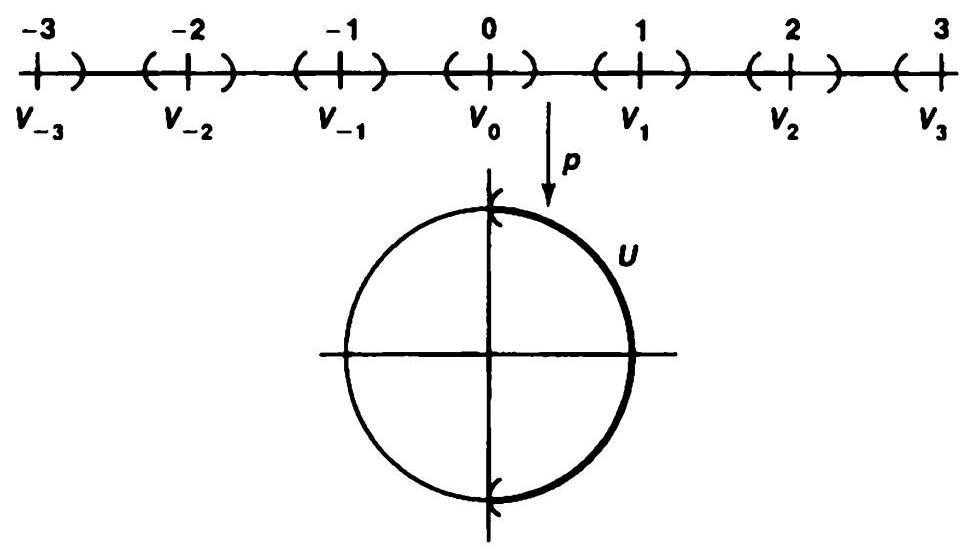
\includegraphics[width=0.8\textwidth]{images/53.2.jpg}
\end{center}
\hspace*{3em} 

Figure 53.2

Similar arguments can be applied to the intersections of \({S}^{1}\) with the upper and lower open half-planes, and with the open left-hand half-plane. These open sets cover \({S}^{1}\) , and each of them is evenly covered by \(p\) . Hence \(p : \mathbb{R} \rightarrow  {S}^{1}\) is a covering map.

If \(p : E \rightarrow  B\) is a covering map, then \(p\) is a \index{Local homeomorphism} of \(E\) with \(B\) . That is, each point \(e\) of \(E\) has a neighborhood that is mapped homeomorphically by \(p\) onto an open subset of \(B\) . The condition that \(p\) be a local homeomorphism does not suffice, however, to ensure that \(p\) is a covering map, as the following example shows.

\begin{centeredblock}
\begin{example}
	The map \(p : {\mathbb{R}}_{ + } \rightarrow  {S}^{1}\) given by the equation

\[
p( x)  = ( {\cos {2\pi x},\sin {2\pi x}})
\]

is surjective, and it is a \index{local homeomorphism@Local homeomorphism}local homeomorphism. See Figure 53.3. But it is not a covering map, for the point \({b}_{0} = ( {1,0})\) has no neighborhood \(U\) that is evenly covered by \(p\) . The typical neighborhood \(U\) of \({b}_{0}\) has an inverse image consisting of small neighborhoods \({V}_{n}\) of each integer \(n\) for \(n > 0\) , along with a small interval \({V}_{0}\) of the form \(( {0,\epsilon })\) . Each of the intervals \({V}_{n}\) for \(n > 0\) is mapped homeomorphically onto \(U\) by the map \(p\) , but the interval \({V}_{0}\) is only imbedded in \(U\) by \(p\) .

\begin{center}
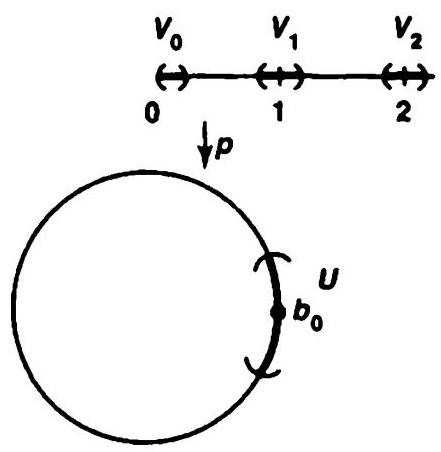
\includegraphics[width=0.4\textwidth]{images/53.3.jpg}
\end{center}
\hspace*{3em} 

Figure 53.3

\end{example}
\end{centeredblock}

\begin{centeredblock}
\begin{example}
	The preceding example might lead you to think that the real line \(\mathbb{R}\) is the only connected covering space of the circle \({S}^{1}\) . This is not so. Consider, for example, the map \(p.{S}^{1} \rightarrow  {S}^{1}\) given in equations by

\[
p( z)  = {z}^{2}.
\]

[Here we consider \({S}^{1}\) as the subset of the complex plane \(\mathbb{C}\) consisting of those complex numbers \(z\) with \(| z|  = 1\) ] We leave it to you to check that \(p\) is a covering map.
\end{example}
\end{centeredblock}

Example 2 shows that the map obtained by restricting a covering map may not be a covering map. Here is one situation where it will be a covering map:
\end{proof}
\begin{theorem}
	Let \(p : E \rightarrow  B\) be a covering map. If \({B}_{0}\) is a subspace of \(B\) , and if \({E}_{0} = {p}^{-1}( {B}_{0})\) , then the map \({p}_{0} : {E}_{0} \rightarrow  {B}_{0}\) obtained by restricting \(p\) is a covering map.
\end{theorem}

\begin{proof}
	Given \({b}_{0} \in  {B}_{0}\) , let \(U\) be an open set in \(B\) containing \({b}_{0}\) that is evenly covered by \(p\) ; let \(\{  {V}_{\alpha }\}\) be a partition of \({p}^{-1}( U)\) into slices. Then \(U \cap  {B}_{0}\) is a neighborhood of \({b}_{0}\) in \({B}_{0}\) , and the sets \({V}_{\alpha } \cap  {E}_{0}\) are disjoint open sets in \({E}_{0}\) whose union is \({p}^{-1}( {U \cap  {B}_{0}})\) , and each is mapped homeomorphically onto \(U \cap  {B}_{0}\) by \(p\) .
\end{proof}
\begin{theorem}
	If \(p : E \rightarrow  B\) and \({p}^{\prime } : {E}^{\prime } \rightarrow  {B}^{\prime }\) are covering maps, then

\[
p \times  {p}^{\prime } : E \times  {E}^{\prime } \rightarrow  B \times  {B}^{\prime }
\]

is a covering map.
\end{theorem}

\begin{proof}
	Given \(b \in  B\) and \({b}^{\prime } \in  {B}^{\prime }\) , let \(U\) and \({U}^{\prime }\) be neighborhoods of \(b\) and \({b}^{\prime }\) , respectively, that are evenly covered by \(p\) and \({p}^{\prime }\) , respectively. Let \(\{  {V}_{\alpha }\}\) and \(\{  {V}_{\beta }^{\prime }\}\) be partitions of \({p}^{-1}( U)\) and \({( {p}^{\prime }) }^{-1}( {U}^{\prime })\) , respectively, into slices. Then the inverse image under \(p \times  {p}^{\prime }\) of the open set \(U \times  {U}^{\prime }\) is the union of all the sets \({V}_{\alpha } \times  {V}_{\beta }^{\prime }\) . These are disjoint open sets of \(E \times  {E}^{\prime }\) , and each is mapped homeomorphically onto \({U}^{\prime } \times  {U}^{\prime }\) by \(p \times  {p}^{\prime }\) .

\begin{centeredblock}
\begin{example}
	Consider the space \(T = {S}^{1} \times  {S}^{1}\) , it is called the torus The product map

\[
p \times  p\mathbb{R} \times  \mathbb{R} \rightarrow  {S}^{1} \times  {S}^{1}
\]

is a covering of the torus by the plane \({\mathbb{R}}^{2}\) , where \(p\) denotes the covering map of Theorem 53 1 Each of the unit squares \([  {n,n + 1}]   \times  [  {m,m + 1}]\) gets wrapped by \(p \times  p\) entirely around the torus. See Figure 534

\begin{center}
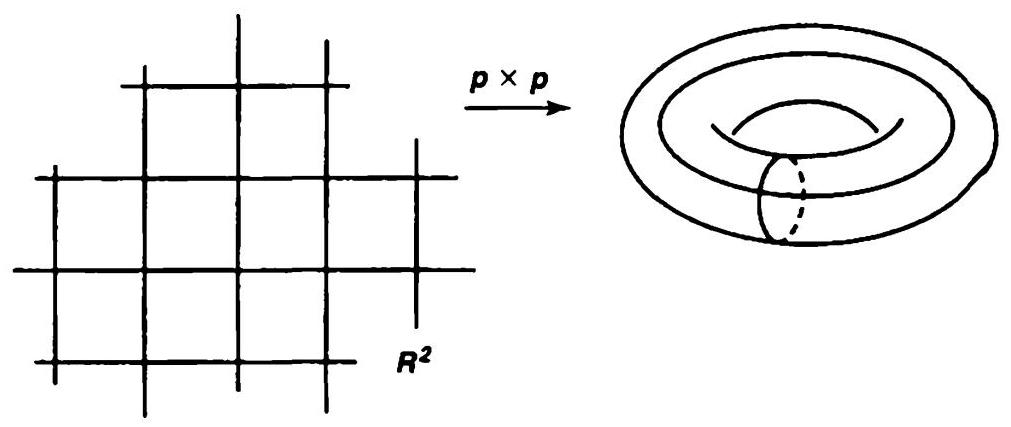
\includegraphics[width=0.9\textwidth]{images/53.4.jpg}
\end{center}
\hspace*{3em} 

Figure 53.4

In this figure, we have pictured the torus not as the product \({S}^{1} \times  {S}^{1}\) , which is a subspace of \({\mathbb{R}}^{4}\) and thus difficult to visualize, but as the familiar doughnut-shaped surface \(D\) in \({\mathbb{R}}^{3}\) obtained by rotating the circle \({C}_{1}\) in the \({xz}\) -plane of radius \(\frac{1}{3}\) centered at(1,0,0)about the \(z\) -axis. It is not hard to see that \({S}^{1} \times  {S}^{1}\) is homeomorphic with the surface \(D\) Let \({C}_{2}\) be the circle of radius 1 in the \({xy}\) -plane centered at the origin. Then let us map \({C}_{1} \times  {C}_{2}\) into \(D\) by defining \(f( {a \times  b})\) to be that point into which \(a\) is carried when one rotates the circle \({C}_{1}\) about the \(z\) -axis until its center hits the point \(b\) See Figure 53.5. The map \(f\) will be a homeomorphism of \({C}_{1} \times  {C}_{2}\) with \(D\) , as you can check mentally. If you wish, you can write equations for \(f\) and check continuity, injectivity, and surjectivity directly. (Continuity of \({f}^{-1}\) will follow from compactness of \({C}_{1} \times  {C}_{2}\) .)

\begin{center}
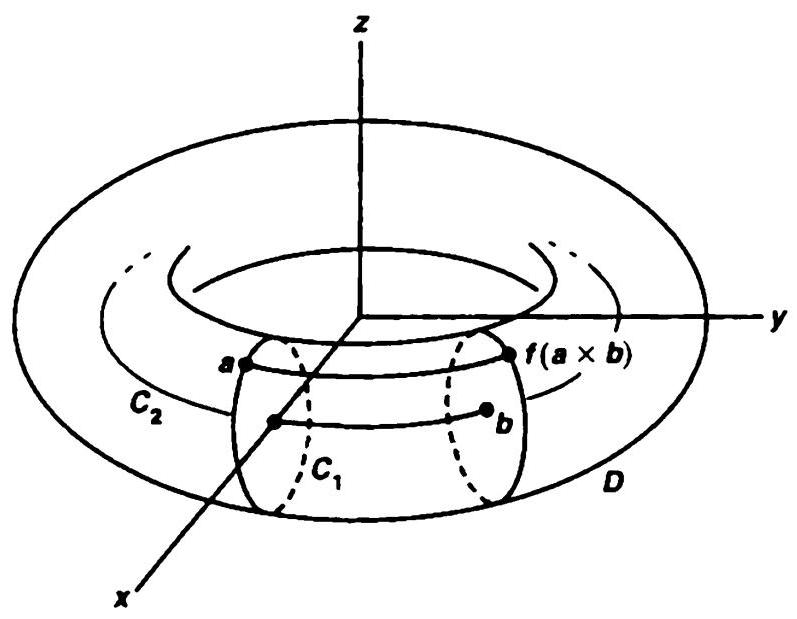
\includegraphics[width=0.7\textwidth]{images/53.5.jpg}
\end{center}
\hspace*{3em} 

Figure 53.5

\end{example}
\end{centeredblock}

\begin{centeredblock}
\begin{example}
	Consider the covering map \(p \times  p\) of the preceding example. Let \({b}_{0}\) denote the point \(p( 0)\) of \({S}^{1}\) ; and let \({B}_{0}\) denote the subspace

\[
{B}_{0} = ( {{S}^{1} \times  {b}_{0}})  \cup  ( {{b}_{0} \times  {S}^{1}})
\]

of \({S}^{1} \times  {S}^{1}\) . Then \({B}_{0}\) is the union of two circles that have a point in common, we sometimes call it the \index{Figure-eight space} The space \({E}_{0} = {p}^{-1}( {B}_{0})\) is the ``infinite grid''

\[
{E}_{0} = ( {\mathbb{R} \times  \mathbb{Z}})  \cup  ( {\mathbb{Z} \times  \mathbb{R}})
\]

pictured in Figure 534. The map \({p}_{0} : {E}_{0} \rightarrow  {B}_{0}\) obtained by restricting \(p \times  p\) is thus a covering map.

The infinite grid is but one \index{Torus!covering space of}covering space of the figure eight; we shall see others later on.

\end{example}
\end{centeredblock}

\begin{centeredblock}
\begin{example}
	Consider the covering map

\[
p \times  i : \mathbb{R} \times  {\mathbb{R}}_{ + } \rightarrow  {S}^{1} \times  {\mathbb{R}}_{ + }
\]

where \(i\) is the identity map of \({\mathbb{R}}_{ + }\) and \(p\) is the map of Theorem 531. If we take the standard homeomorphism of \({S}^{1} \times  {\mathbb{R}}_{ + }\) with \({\mathbb{R}}^{2} - \mathbf{0}\) , sending \(x \times  t\) to \({tx}\) , the composite gives us a covering

\[
\mathbb{R} \times  {\mathbb{R}}_{ + } \rightarrow  {\mathbb{R}}^{2} - 0
\]

of the punctured plane by the open upper half-plane. It is pictured in Figure S3.6. This covering map appears in the study of complex variables as the Riemann surface corresponding to the complex logarithm function.

\begin{center}
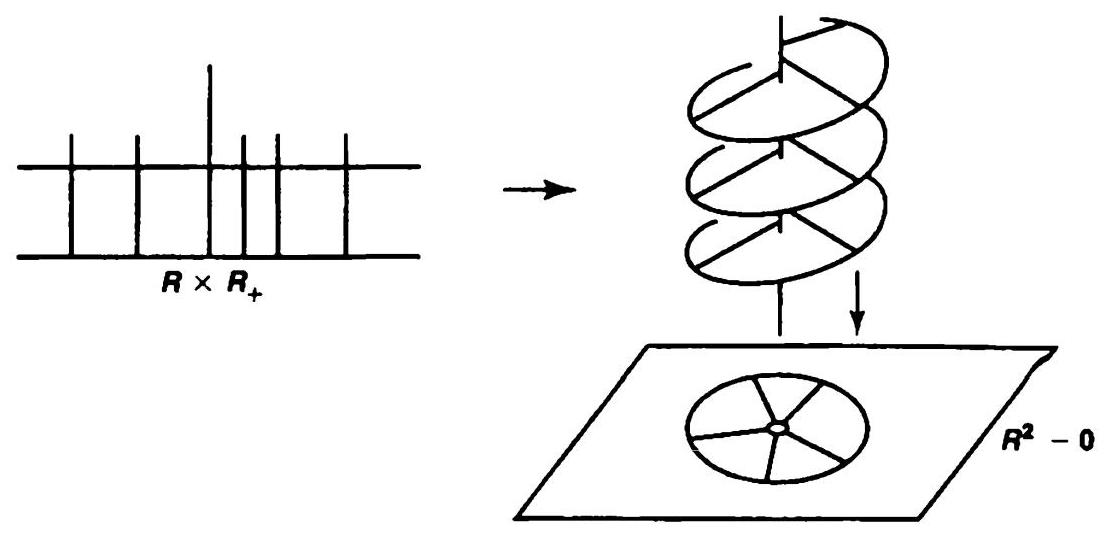
\includegraphics[width=1.0\textwidth]{images/53.6.jpg}
\end{center}
\hspace*{3em} 

Figure 53.6
\end{example}
\end{centeredblock}
\end{proof}
\section*{Exercises}
\begin{enumerate}[itemsep=0.4em, parsep=0pt, topsep=0pt, partopsep=0pt, leftmargin=*, label=\arabic*., ref=\arabic*]
\item Let \(Y\) have the discrete topology. Show that if \(p : X \times  Y \rightarrow  X\) is projection on the first coordinate, then \(p\) is a covering map.
\item Let \(p : E \rightarrow  B\) be continuous and surjective. Suppose that \(U\) is an open set of \(B\) that is evenly covered by \(p\) . Show that if \(U\) is connected, then the partition of \({p}^{-1}( U)\) into slices is unique.
\item Let \(p : E \rightarrow  B\) be a covering map; let \(B\) be connected. Show that if \({p}^{-1}( {b}_{0})\) has \(k\) elements for some \({b}_{0} \in  B\) , then \({p}^{-1}( b)\) has \(k\) elements for every \(b \in  B\) . In such a case, \(E\) is called a \(k\) -fold covering of \(B\) .
\item Let \(q : X \rightarrow  Y\) and \(r : Y \rightarrow  Z\) be covering maps; let \(p = r \circ  q\) . Show that if \({r}^{-1}( z)\) is finite for each \(z \in  Z\) , then \(p\) is a covering map.
\item Show that the map of Example 3 is a covering map. Generalize to the map \(p( z)  = {z}^{n}.\)
\item Let \(p : E \rightarrow  B\) be a covering map.
  \begin{enumerate}[itemsep=0.2em, parsep=0pt, topsep=0pt, partopsep=0pt, leftmargin=*, label=(\alph*), align=left]
  \item If \(B\) is Hausdorff, regular, completely regular, or locally compact Hausdorff, then so is \(E\) . [Hint: If \(\{  {V}_{\alpha }\}\) is a partition of \({p}^{-1}( U)\) into slices, and \(C\) is a closed set of \(B\) such that \(C \subset  U\) , then \({p}^{-1}( C)  \cap  {V}_{\alpha }\) is a closed set of \(E\) .]
  \item If \(B\) is compact and \({p}^{-1}( b)\) is finite for each \(b \in  B\) , then \(E\) is compact.
  \end{enumerate}
\end{enumerate}
\section*{§ 54 The Fundamental Group of the Circle}

The study of covering spaces of a space \(X\) is intimately related to the study of the fundamental group of \(X\) . In this section, we establish the crucial links between the two concepts, and compute the fundamental group of the circle.

\begin{definition}
	Let \(p : E \rightarrow  B\) be a map. If \(f\) is a continuous mapping of some space \(X\) into \(B\) , a \index{Lifting} of \(f\) is a map \(\bar{f} : X \rightarrow  E\) such that \(p \circ  \bar{f} = f\) .
\end{definition}

\begin{center}
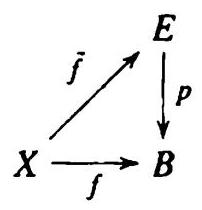
\includegraphics[width=0.2\textwidth]{images/54.0.jpg}
\end{center}
\hspace*{3em} 

The existence of \index{lifting@Lifting}liftings when \(p\) is a covering map is an important tool in studying covering spaces and the fundamental group. First, we show that for a covering space, paths can be lifted; then we show that path homotopies can be lifted as well. First, an example:

\begin{centeredblock}
\begin{example}
	Consider the covering \(p\mathbb{R} \rightarrow  {S}^{1}\) of Theorem 53.1. The path \(f\) . \([  {0,1}]   \rightarrow  {S}^{1}\) beginning at \({b}_{0} = ( {1,0})\) given by \(f( s)  = ( {\cos {\pi s},\sin {\pi s}})\) lifts to the path \(\bar{f}( s)  = s/2\) beginning at 0 and ending at \(\frac{1}{2}\) . The path \(g( s)  = ( {\cos {\pi s}, - \sin {\pi s}})\) lifts to the path \(\bar{g}( s)  =  - s/2\) beginning at 0 and ending at \(- \frac{1}{2}\) The path \(h( s)  = ( {\cos {4\pi s},\sin {4\pi s}})\) lifts to the path \(\bar{h}( s)  = {2s}\) beginning at 0 and ending at 2 . Intuitively, \(h\) wraps the interval \([  {0,1}]\) around the circle twice; this is reflected in the fact that the lifted path \(\bar{h}\) begins at zero and ends at the number 2 These paths are pictured in Figure 541.

\begin{center}
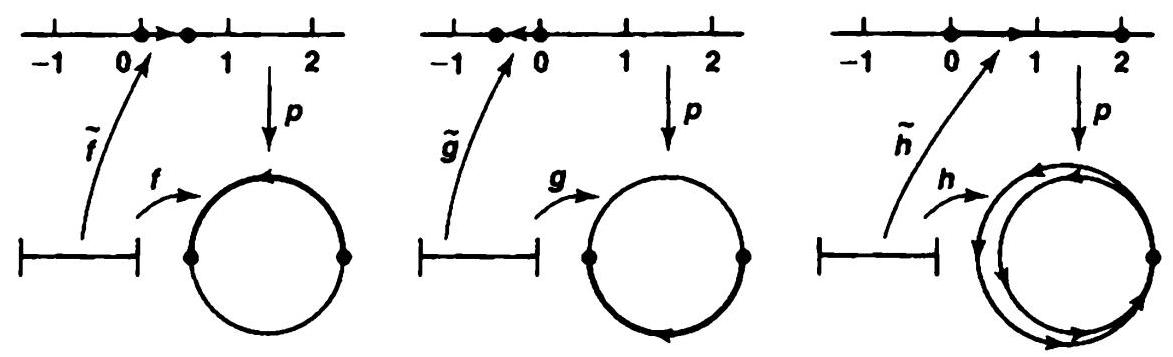
\includegraphics[width=1.0\textwidth]{images/54.1.jpg}
\end{center}
\hspace*{3em} 

Figure 54.1

\begin{lemma}
	Let \(p : E \rightarrow  B\) be a covering map, let \(p( {e}_{0})  = {b}_{0}\) . Any path \(f.[  {0,1}]   \rightarrow  B\) beginning at \({b}_{0}\) has a unique lifting to a path \(\bar{f}\) in \(E\) beginning at \({e}_{0}\) .
\end{lemma}

\begin{proof}
	Cover \(B\) by open sets \(U\) each of which is evenly covered by \(p\) . Find a subdivision of \([  {0,1}]\) , say \({s}_{0},\ldots ,{s}_{n}\) , such that for each \(i\) the set \(f( [  {{s}_{i},{s}_{i + 1}}]  )\) lies in such an open set \(U\) . (Here we use the Lebesgue number lemma.) We define the lifting \(\bar{f}\) step by step.
First, define \(\bar{f}( 0)  = {e}_{0}\) . Then, supposing \(\bar{f}( s)\) is defined for \(0 \leq  s \leq  {s}_{i}\) , we define \(\widetilde{f}\) on \([  {{s}_{i},{s}_{i + 1}}]\) as follows: The set \(f( [  {{s}_{i},{s}_{i + 1}}]  )\) lies in some open set \(U\) that is evenly covered by \(p\) Let \(\{  {V}_{\alpha }]\) be a partition of \({p}^{-1}( U)\) into slices; each set \({V}_{\alpha }\) is mapped homeomorphically onto \(U\) by \(p\) . Now \(\widetilde{f}( {s}_{i})\) lies in one of these sets, say in \({V}_{0}\) . Define \(\bar{f}( s)\) for \(s \in  [  {{s}_{i},{s}_{i + 1}}]\) by the equation

\[
\bar{f}( s)  = {( p \mid  {V}_{0}) }^{-1}( {f( s) }) .
\]

Because \(p \mid  {V}_{0} : {V}_{0} \rightarrow  U\) is a homeomorphism, \(\widetilde{f}\) will be continuous on \([  {{s}_{i},{s}_{i + 1}}]\) .

Continuing in this way, we define \(\widetilde{f}\) on all of \([  {0,1}]\) . Continuity of \(\widetilde{f}\) follows from the pasting lemma; the fact that \(p \circ  \bar{f} = f\) is immediate from the definition of \(\bar{f}\) .

The uniqueness of \(\bar{f}\) is also proved step by step. Suppose that \(\bar{\bar{f}}\) is another lifting of \(f\) beginning at \({e}_{0}\) . Then \(\widetilde{\widetilde{f}}( 0)  = {e}_{0} = \bar{f}( 0)\) . Suppose that \(\overline{\widetilde{f}}( s)  = \widetilde{f}( s)\) for all \(s\) such that \(0 \leq  s \leq  {s}_{i}\) . Let \({V}_{0}\) be as in the preceding paragraph; then for \(s \in  [  {{s}_{i},{s}_{t + 1}}]\) , \(\widetilde{f}( s)\) is defined as \({( p \mid  {V}_{0}) }^{-1}( {f( s) })\) . What can \(\overline{\bar{f}}( s)\) equal? Since \(\overline{\bar{f}}\) is a lifting of \(f\) , it must carry the interval \([  {{s}_{i},{s}_{i + 1}}]\) into the set \({p}^{-1}( U)  = \bigcup {V}_{\alpha }\) . The slices \({V}_{\alpha }\) are open and disjoint; because the set \(\widetilde{\widetilde{f}}( [  {{s}_{i},{s}_{i + 1}}]  )\) is connected, it must lie entirely in one of the sets \({V}_{\alpha }\) . Because \(\widetilde{\bar{f}}( {s}_{i})  = \widetilde{f}( {s}_{i})\) , which is in \({V}_{0},\bar{\bar{f}}\) must carry all of \([  {{s}_{i},{s}_{i + 1}}]\) into the set \({V}_{0}\) . Thus, for \(s\) in \([  {{s}_{i},{s}_{i + 1}}]  ,\widetilde{\bar{f}}( s)\) must equal some point \(y\) of \({V}_{0}\) lying in \({p}^{-1}( {f( s) })\) . But there is only one such point \(y\) , namely, \({( p \mid  {V}_{0}) }^{-1}( {f( s) })\) . Hence \(\widetilde{\widetilde{f}}( s)  = \widetilde{f}( s)\) for \(s \in  [  {{s}_{i},{s}_{i + 1}}]\)
\end{proof}
\begin{lemma}
	Let \(p : E \rightarrow  B\) be a covering map; let \(p( {e}_{0})  = {b}_{0}\) . Let the map \(F : I \times  I \rightarrow  B\) be continuous, with \(F( {0,0})  = {b}_{0}\) . There is a unique lifting of \(F\) to a continuous map

\[
\widetilde{F} : I \times  I \rightarrow  E
\]

such that \(\bar{F}( {0,0})  = {e}_{0}\) . If \(F\) is a path homotopy, then \(\widetilde{F}\) is a path homotopy.
\end{lemma}

\begin{proof}
	Given \(F\) , we first define \(\bar{F}( {0,0})  = {e}_{0}\) . Next, we use the preceding lemma to extend \(\bar{F}\) to the left-hand edge \(0 \times  I\) and the bottom edge \(I \times  0\) of \(I \times  I\) . Then we extend \(\bar{F}\) to all of \(I \times  I\) as follows:
Choose subdivisions

\[
{s}_{0} < {s}_{1} < \cdots  < {s}_{m}
\]

\[
{t}_{0} < {t}_{1} < \cdots  < {t}_{n}
\]

of \(I\) fine enough that each rectangle

\[
{I}_{i} \times  {J}_{j} = [  {{s}_{i - 1},{s}_{i}}]   \times  [  {{t}_{j - 1},{t}_{j}}\}
\]

is mapped by \(F\) into an open set of \(B\) that is evenly covered by \(p\) . (Use the Lebesgue number lemma.) We define the lifting \(\widetilde{F}\) step by step, beginning with the rectangle \({I}_{1} \times  {J}_{1}\) , continuing with the other rectangles \({I}_{t} \times  {J}_{1}\) in the ``bottom row,'' then with the rectangles \({I}_{i} \times  {J}_{2}\) in the next row, and so on.

In general, given \({i}_{0}\) and \({j}_{0}\) , assume that \(\widetilde{F}\) is defined on the set \(A\) which is the union of \(0 \times  I\) and \(I \times  0\) and all the rectangles ``previous'' to \({I}_{{i}_{0}} \times  {J}_{J0}\) (those rectangles \({I}_{i} \times  {J}_{j}\) for which \(j < {j}_{0}\) and those for which \(j = {j}_{0}\) and \(i < {i}_{0}\) ). Assume also that \(\bar{F}\) is a continuous lifting of \(F \mid  A\) . We define \(\bar{F}\) on \({I}_{{i}_{0}} \times  {J}_{{j}_{0}}\) . Choose an open set \(U\) of \(B\) that is evenly covered by \(p\) and contains the set \(F( {{I}_{{t}_{0}} \times  {J}_{{j}_{0}}})\) . Let \(\{  {V}_{\alpha }\}\) be a partition of \({p}^{-1}( U)\) into slices; each set \({V}_{\alpha }\) is mapped homeomorphically onto \(U\) by \(p\) . Now \(\bar{F}\) is already defined on the set \(C = A \cap  ( {{I}_{{i}_{0}} \times  {J}_{{j}_{0}}})\) . This set is the union of the left and bottom edges of the rectangle \({I}_{{i}_{0}} \times  {J}_{{j}_{0}}\) , so it is connected. Therefore, \(\bar{F}( C)\) is connected and must lie entirely within one of the sets \({V}_{\alpha }\) . Suppose it lies in \({V}_{0}\) Then, the situation is as pictured in Figure 54.2.

\begin{center}
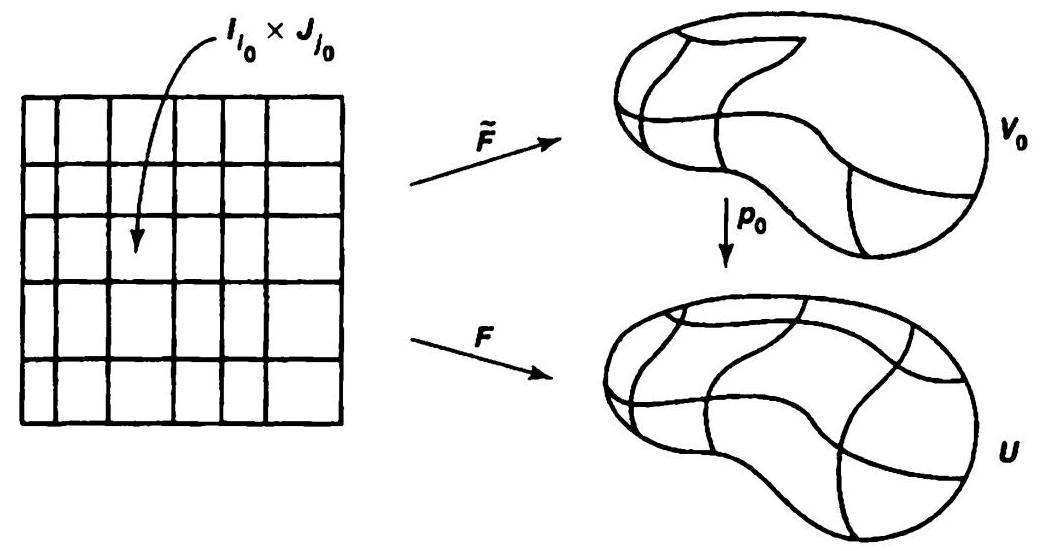
\includegraphics[width=0.9\textwidth]{images/54.2.jpg}
\end{center}
\hspace*{3em} 

Figure 54.2

Let \({p}_{0} : {V}_{0} \rightarrow  U\) denote the restriction of \(p\) to \({V}_{0}\) . Since \(\bar{F}\) is a lifting of \(F \mid  A\) , we know that for \(x \in  C\) ,

\[
{p}_{0}( {\widetilde{F}( x) })  = p( {\bar{F}( x) })  = F( x) ,
\]

so that \(\widetilde{F}( x)  = {p}_{0}^{-1}( {F( x) })\) . Hence we may extend \(\widetilde{F}\) by defining

\[
\widetilde{F}( x)  = {p}_{0}^{-1}( {F( x) })
\]

for \(x \in  {I}_{{i}_{0}} \times  {J}_{{j}_{0}}\) . The extended map will be continuous by the pasting lemma.

Continuing in this way, we define \(\widetilde{F}\) on all of \({I}^{2}\) .

To check uniqueness, note that at each step of the construction of \(\bar{F}\) , as we extend \(\widetilde{F}\) first to the bottom and left edges of \({I}^{2}\) , and then to the rectangles \({I}_{i} \times  {J}_{j}\) , one by one, there is only one way to extend \(\bar{F}\) continuously. Thus, once the value of \(\bar{F}\) at (0,0)is specified, \(\bar{F}\) is completely determined.

Now suppose that \(F\) is a path homotopy. We wish to show that \(\widetilde{F}\) is a path homotopy. The map \(F\) carries the entire left edge \(0 \times  I\) of \({I}^{2}\) into a single point \({b}_{0}\) of \(B\) . Because \(\widetilde{F}\) is a lifting of \(F\) , it carries this edge into the set \({p}^{-1}( {b}_{0})\) . But this set has the discrete topology as a subspace of \(E\) . Since \(0 \times  I\) is connected and \(\widetilde{F}\) is continuous, \(\bar{F}( {0 \times  I})\) is connected and thus must equal a one-point set. Similarly, \(\bar{F}( {1 \times  I})\) must be a one-point set. Thus \(\bar{F}\) is a path homotopy.
\end{proof}
\begin{theorem}
	Let \(p : E \rightarrow  B\) be a covering map; let \(p( {e}_{0})  = {b}_{0}\) . Let \(f\) and \(g\) be two paths in \(B\) from \({b}_{0}\) to \({b}_{1}\) , let \(\widetilde{f}\) and \(\widetilde{g}\) be their respective liftings to paths in \(E\) beginning at \({e}_{0}\) . If \(f\) and \(g\) are path homotopic, then \(\widetilde{f}\) and \(\widetilde{g}\) end at the same point of \(E\) and are path homotopic.
\end{theorem}
\begin{proof}
	Let \(F : I \times  I \rightarrow  B\) be the path homotopy between \(f\) and \(g\) . Then \(F( {0,0})  =\)  \({b}_{0}\) Let \(\bar{F} : I \times  I \rightarrow  E\) be the lifting of \(F\) to \(E\) such that \(\bar{F}( {0,0})  = {e}_{0}\) . By the preceding lemma, \(\bar{F}\) is a path homotopy, so that \(\bar{F}( {0 \times  I})  = \{  {e}_{0}]\) and \(\bar{F}( {1 \times  I})\) is a one-point set \(\{  {e}_{1}]\)

The restriction \(\bar{F} \mid  I \times  0\) of \(\bar{F}\) to the bottom edge of \(I \times  I\) is a path on \(E\) beginning at \({e}_{0}\) that is a lifting of \(F \mid  I \times  0\) . By uniqueness of path liftings, we must have \(\bar{F}( {s,0})  =\)  \(\widetilde{f}( s)\) . Similarly, \(\bar{F} \mid  I \times  1\) is a path on \(E\) that is a lifting of \(F \mid  I \times  1\) , and it begins at \({e}_{0}\) because \(\bar{F}( {0 \times  I})  = \{  {e}_{0}]\) . By uniqueness of path liftings, \(\bar{F}( {s,1})  = \widetilde{g}( s)\) Therefore, both \(\bar{f}\) and \(\bar{g}\) end at \({e}_{1}\) , and \(\bar{F}\) is a path homotopy between them.
\end{proof}

\begin{definition}
	Let \(p : E \rightarrow  B\) be a covering map; let \({b}_{0} \in  B\) Choose \({e}_{0}\) so that \(p( {e}_{0})  = {b}_{0}\) . Given an element \([  f]\) of \({\pi }_{1}( {B,{b}_{0}})\) , let \(\bar{f}\) be the lifting of \(f\) to a path in \(E\) that begins at \({e}_{0}\) . Let \(\phi ( [  f]  )\) denote the end point \(\widetilde{f}( 1)\) of \(\widetilde{f}\) . Then \(\phi\) is a well-defined set map

\[
\phi  : {\pi }_{1}( {B,{b}_{0}})  \rightarrow  {p}^{-1}( {b}_{0}) .
\]

We call \(\phi\) the \index{Lifting correspondence} derived from the covering map \(p\) . It depends of course on the choice of the point \({e}_{0}\) .
\end{definition}

\begin{theorem}
	Let \(p : E \rightarrow  B\) be a covering map; let \(p( {e}_{0})  = {b}_{0}\) . If \(E\) is path connected, then the \index{lifting correspondence@Lifting correspondence}lifting correspondence

\[
\phi  : {\pi }_{1}( {B,{b}_{0}})  \rightarrow  {p}^{-1}( {b}_{0})
\]

is surjective. If \(E\) is simply connected, it is bijective.
\end{theorem}

\begin{proof}
	If \(E\) is path connected, then, given \({e}_{1} \in  {p}^{-1}( {b}_{0})\) , there is a path \(\bar{f}\) in \(E\) from \({e}_{0}\) to \({e}_{1}\) . Then \(f = p \circ  \widetilde{f}\) is a loop in \(B\) at \({b}_{0}\) , and \(\phi ( [  f]  )  = {e}_{1}\) by definition
Suppose \(E\) is simply connected. Let \([  f]\) and \([  g]\) be two elements of \({\pi }_{1}( {B,{b}_{0}})\) such that \(\phi ( [  f]  )  = \phi ( [  g]  )\) . Let \(\bar{f}\) and \(\bar{g}\) be the liftings of \(f\) and \(g\) , respectively, to paths in \(E\) that begin at \({e}_{0}\) , then \(\widetilde{f}( 1)  = \widetilde{g}( 1)\) . Since \(E\) is simply connected, there is a path homotopy \(\widetilde{F}\) in \(E\) between \(\widetilde{f}\) and \(\bar{g}\) . Then \(p \circ  \widetilde{F}\) is a path homotopy in \(B\) between \(f\) and \(g\)
\end{proof}
\begin{theorem}
	The \index{Fundamental group!of \({S}^{1}\)}fundamental group of \({S}^{1}\) is isomorphic to the additive group of integers.
\end{theorem}

\begin{proof}
	Let \(p : \mathbb{R} \rightarrow  {S}^{1}\) be the covering map of Theorem 53.1, let \({e}_{0} = 0\) , and let \({b}_{0} = p( {e}_{0})\) . Then \({p}^{-1}( {b}_{0})\) is the set \(\mathbb{Z}\) of integers. Since \(\mathbb{R}\) is simply connected, the lifting correspondence
\[
\phi  : {\pi }_{1}( {{S}^{1},{b}_{0}})  \rightarrow  \mathbb{Z}
\]

is bijective. We show that \(\phi\) is a homomorphism, and the theorem is proved.

Given \([  f]\) and \([  g]\) in \({\pi }_{1}( {B,{b}_{0}})\) , let \(\widetilde{f}\) and \(\widetilde{g}\) be their respective liftings to paths on \(\mathbb{R}\) beginning at 0 . Let \(n = \widetilde{f}( 1)\) and \(m = \widetilde{g}( 1)\) ; then \(\phi ( [  f]  )  = n\) and \(\phi ( [  g]  )  = m\) , by definition. Let \(\widetilde{\widetilde{g}}\) be the path

\[
\widetilde{\bar{g}}( s)  = n + \widetilde{g}( s)
\]

on \(\mathbb{R}\) . Because \(p( {n + x})  = p( x)\) for all \(x \in  \mathbb{R}\) , the path \(\widetilde{g}\) is a lifting of \(g\) ; it begins at \(n\) . Then the product \(\widetilde{f} * \overline{\widetilde{g}}\) is defined, and it is the lifting of \(f * g\) that begins at 0, as you can check. The end point of this path is \(\widetilde{\widetilde{g}}( 1)  = n + m\) . Then by definition,

\[
\phi ( {[  f]   * [  g]  })  = n + m = \phi ( [  f]  )  + \phi ( [  g]  ) .
\]
\end{proof}
\begin{definition}
	Let \(G\) be a group; let \(x\) be an element of \(G\) . We denote the inverse of \(x\) by \({x}^{-1}\) . The symbol \({x}^{n}\) denotes the \(n\) -fold product of \(x\) with itself, \({x}^{-n}\) denotes the \(n\) -fold product of \({x}^{-1}\) with itself, and \({x}^{0}\) denotes the identity element of \(G\) . If the set of all elements of the form \({x}^{m}\) , for \(m \in  \mathbb{Z}\) , equals \(G\) , then \(G\) is said to be a \index{Cyclic group}, and \(x\) is said to be a \index{generator of cyclic group@Generator of cyclic group} generator of \(G\) .
\end{definition}

The cardinality of a group is also called the \index{order of a group@Order of a group} order of the group. A group is cyclic of infinite order if and only if it is isomorphic to the additive group of integers; it is cyclic of order \(k\) if and only if it is isomorphic to the group \(\mathbb{Z}/k\) of integers modulo \(k\) . The preceding theorem implies that the fundamental group of the circle is infinite cyclic.

Note that if \(x\) is a generator of the infinite cyclic group \(G\) , and if \(y\) is an element of the arbitrary group \(H\) , then there is a unique homomorphism \(h\) of \(G\) into \(H\) such that \(h( x)  = y\) ; it is defined by setting \(h( {x}^{n})  = {y}^{n}\) for all \(n\) .

For later use, in §65 and in Chapters 13 and 14, we prove here a strengthened version of Theorem 54.4.

-Theorem 54.6. Let \(p : E \rightarrow  B\) be a covering map; let \(p( {e}_{0})  = {b}_{0}\) .

(a) The homomorphism \({p}_{ * } : {\pi }_{1}( {E,{e}_{0}})  \rightarrow  {\pi }_{1}( {B,{b}_{0}})\) is a \index{monomorphism@Monomorphism}monomorphism.

(b) Let \(H = {p}_{ * }( {{\pi }_{1}( {E,{e}_{0}}) })\) . The lifting correspondence \(\phi\) induces an injective map

\[
\Phi  : {\pi }_{1}( {B,{b}_{0}}) /H \rightarrow  {p}^{-1}( {b}_{0})
\]

of the collection of right cosets of \(H\) into \({p}^{-1}( {b}_{0})\) , which is bijective if \(E\) is path connected.

(c) If \(f\) is a loop in \(B\) based at \({b}_{0}\) , then \([  f]   \in  H\) if and only if \(f\) lifts to a loop in \(E\) based at \({e}_{0}\) .

\begin{proof}
	(a) Suppose \(\widetilde{h}\) is a loop in \(E\) at \({e}_{0}\) , and \({p}_{ * }( [  \widetilde{h}]  )\) is the identity element. Let \(F\) be a path homotopy between \(p \circ  \widetilde{h}\) and the constant loop. If \(\widetilde{F}\) is the lifting of \(F\) to \(E\) such that \(\widetilde{F}( {0,0})  = {e}_{0}\) , then \(\bar{F}\) is a path homotopy between \(\bar{h}\) and the constant loop at \({e}_{0}\) .
(b) Given loops \(f\) and \(g\) in \(B\) , let \(\bar{f}\) and \(\bar{g}\) be liftings of them to \(E\) that begin at \({e}_{0}\) . Then \(\phi ( [  f]  )  = \bar{f}( 1)\) and \(\phi ( [  g]  )  = \bar{g}( 1)\) . We show that \(\phi ( [  f]  )  = \phi ( [  g]  )\) if and only if \([  f]   \in  H * [  g]\) .

First, suppose that \([  f]   \in  H * [  g]\) . Then \([  f]   = [  {h * g}]\) , where \(h = p \circ  \bar{h}\) for some loop \(\widetilde{h}\) in \(E\) based at \({e}_{0}\) . Now the product \(\bar{h} * \widetilde{g}\) is defined, and it is a lifting of \(h * g\) . Because \([  f]   = [  {h * g}]\) , the liftings \(\bar{f}\) and \(\bar{h} * \widetilde{g}\) , which begin at \({e}_{0}\) , must end at the same point of \(E\) . Then \(\bar{f}\) and \(\widetilde{g}\) end at the same point of \(E\) , so that \(\phi ( [  f]  )  = \phi ( [  g]  )\) . See Figure 54.3.

\begin{center}
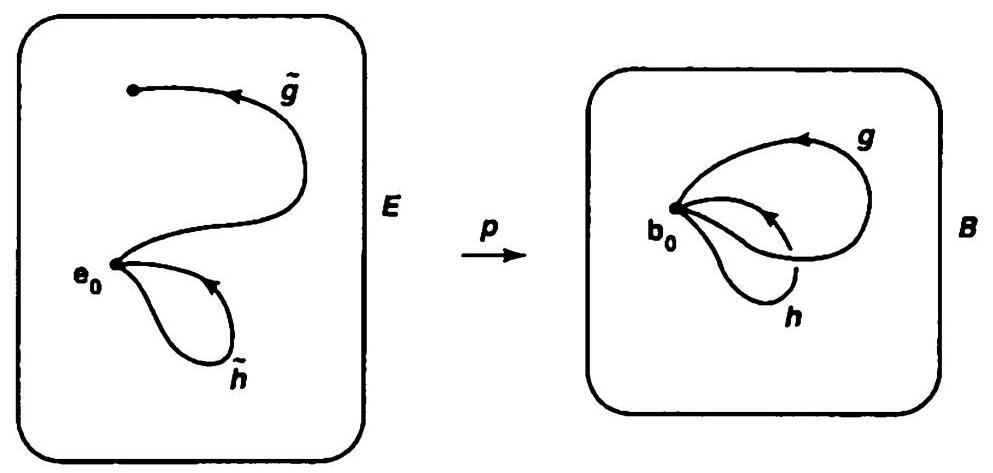
\includegraphics[width=0.9\textwidth]{images/54.3.jpg}
\end{center}
\hspace*{3em} 

Figure 54.3

Now suppose that \(\phi ( [  f]  )  = \phi ( [  g]  )\) . Then \(\bar{f}\) and \(\widetilde{g}\) end at the same point of \(E\) . The product of \(\widetilde{f}\) and the reverse of \(\widetilde{g}\) is defined, and it is a loop \(\widetilde{h}\) in \(E\) based at \({e}_{0}\) . By direct computation, \([  {\widetilde{h} * \widetilde{g}}]   = [  \bar{f}]\) . If \(\bar{F}\) is a path homotopy in \(E\) between the loops \(\widetilde{h} * \widetilde{g}\) and \(\widetilde{f}\) , then \(p \circ  \bar{F}\) is a path homotopy in \(B\) between \(h * g\) and \(f\) , where \(h = p \circ  \widetilde{h}\) . Thus \([  f]   \in  H * [  g]\) , as desired.

If \(E\) is path connected, then \(\phi\) is surjective, so that \(\Phi\) is surjective as well.

(c) Injectivity of \(\Phi\) means that \(\phi ( [  f]  )  = \phi ( [  g]  )\) if and only if \([  f]   \in  H * [  g]\) . Applying this result in the case where \(g\) is the constant loop, we see that \(\phi ( [  f]  )  = {e}_{0}\) if and only if \([  f]   \in  H\) . But \(\phi ( [  f]  )  = {e}_{0}\) precisely when the lift of \(f\) that begins at \({e}_{0}\) also ends at \({e}_{0}\) .
\end{proof}
\section*{Exercises}
\begin{enumerate}[itemsep=0.4em, parsep=0pt, topsep=0pt, partopsep=0pt, leftmargin=*, label=\arabic*., ref=\arabic*]
\item What goes wrong with the ``path-lifting lemma'' (Lemma 54.1) for the local homeomorphism of Example 2 of §53?
\item In defining the map \(\bar{F}\) in the proof of Lemma 54.2, why were we so careful about the order in which we considered the small rectangles?
\item Let \(p : E \rightarrow  B\) be a covering map. Let \(\alpha\) and \(\beta\) be paths in \(B\) with \(\alpha ( 1)  = \beta ( 0)\) ; let \(\bar{\alpha }\) and \(\bar{\beta }\) be liftings of them such that \(\widetilde{\alpha }( 1)  = \widetilde{\beta }( 0)\) . Show that \(\bar{\alpha } * \bar{\beta }\) is a lifting of \(\alpha  * \beta\) .
\item Consider the covering map \(p : \mathbb{R} \times  {\mathbb{R}}_{ + } \rightarrow  {\mathbb{R}}^{2} - 0\) of Example 6 of \(§{53}\) . Find liftings of the paths \[ f( t)  = ( {2 - t,0}) , \] \[ g( t)  = ( {( {1 + t}) \cos {2\pi t},( {1 + t}) \sin {2\pi t}}) \] \[ h( t)  = f * g. \] Sketch these paths and their liftings.
\item Consider the covering map \(p \times  p : \mathbb{R} \times  \mathbb{R} \rightarrow  {S}^{1} \times  {S}^{1}\) of Example 4 of \(§{53}\) . Consider the path \[ f( t)  = ( {\cos {2\pi t},\sin {2\pi t}})  \times  ( {\cos {4\pi t},\sin {4\pi t}}) \] in \({S}^{1} \times  {S}^{1}\) . Sketch what \(f\) looks like when \({S}^{1} \times  {S}^{1}\) is identified with the doughnut surface \(D\) . Find a lifting \(\bar{f}\) of \(f\) to \(\mathbb{R} \times  \mathbb{R}\) , and sketch it.
\item Consider the maps \(g,h : {S}^{1} \rightarrow  {S}^{1}\) given \(g( z)  = {z}^{n}\) and \(h( z)  = 1/{z}^{n}\) . (Here we represent \({S}^{1}\) as the set of complex numbers \(z\) of absolute value 1 .) Compute the induced homomorphisms \({g}_{ * },{h}_{ * }\) of the infinite \index{cyclic group@Cyclic group}cyclic group \({\pi }_{1}( {{S}^{1},{b}_{0}})\) into itself. [Hint: Recall the equation \({( \cos \theta  + i\sin \theta ) }^{n} = \cos {n\theta } + i\sin {n\theta }\) .]
\item Generalize the proof of Theorem 54.5 to show that the fundamental group of the torus is isomorphic to the group \(\mathbb{Z} \times  \mathbb{Z}\) .
\item Let \(p : E \rightarrow  B\) be a covering map, with \(E\) path connected. Show that if \(B\) is simply connected, then \(p\) is a homeomorphism.
\end{enumerate}
\section*{§ 55 Retractions and Fixed Points}

We now prove several classical results of topology that follow from our knowledge of the fundamental group of \({S}^{1}\) .

\begin{definition}
	If \(A \subset  X\) , a retraction of \(X\) onto \(A\) is a continuous map \(r : X \rightarrow  A\) such that \(r \mid  A\) is the identity map of \(A\) . If such a map \(r\) exists, we say that \(A\) is a retract of \(X\) .
\end{definition}

\begin{lemma}
	If \(A\) is a retract of \(X\) , then the homomorphism of fundamental groups induced by inclusion \(j : A \rightarrow  X\) is injective.
\end{lemma}

\begin{proof}
	If \(r : X \rightarrow  A\) is a retraction, then the composite map \(r \circ  j\) equals the identity map of \(A\) . It follows that \({r}_{ * } \circ  {j}_{ * }\) is the identity map of \({\pi }_{1}( {A,a})\) , so that \({j}_{ * }\) must be injective.
\end{proof}
\begin{theorem}[\index{no-retraction theorem@No-retraction theorem}]
	There is no retraction of \({B}^{2}\) onto \({S}^{1}\) .
\end{theorem}

\begin{proof}
	If \({S}^{1}\) were a retract of \({B}^{2}\) , then the homomorphism induced by inclusion \(j : {S}^{1} \rightarrow  {B}^{2}\) would be injective. But the fundamental group of \({S}^{1}\) is nontrivial and the \index{B^n@\({B}^{n}\)!fundamental group}fundamental group of \({B}^{2}\) is trivial.
\end{proof}
\begin{lemma}
	Let \(h : {S}^{1} \rightarrow  X\) be a continuous map Then the following conditions are equivalent:

(I) \(h\) is nulhomotopic.

(2) \(h\) extends to a continuous map \(k : {B}^{2} \rightarrow  X\) .

(3) \({h}_{ * }\) is the \index{trivial homomorphism@Trivial homomorphism}trivial homomorphism of fundamental groups.
\end{lemma}

\begin{proof}
	(1) \(\Rightarrow\) (2). Let \(H : {S}^{1} \times  I \rightarrow  X\) be a homotopy between \(h\) and a constant map. Let \(\pi  : {S}^{1} \times  I \rightarrow  {B}^{2}\) be the map
\[
\pi ( {x,t})  = ( {1 - t}) x.
\]

Then \(\pi\) is continuous, closed and surjective, so it is a quotient map; it collapses \({S}^{1} \times  1\) to the point0and is otherwise injective. Because \(H\) is constant on \({S}^{1} \times  1\) , it induces, via the quotient map \(\pi\) , a continuous map \(k : {B}^{2} \rightarrow  X\) that is an extension of \(h\) . See Figure 55.1.

\begin{center}
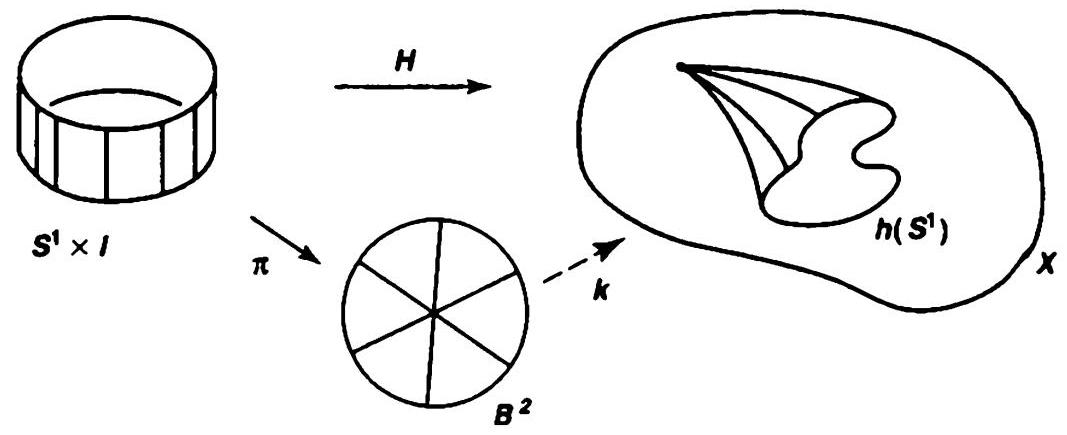
\includegraphics[width=0.9\textwidth]{images/55.1.jpg}
\end{center}
\hspace*{3em} 

Figure 55.1

\(( 2)  \Rightarrow  ( 3)\) . If \(j : {S}^{1} \rightarrow  {B}^{2}\) is the inclusion map, then \(h\) equals the composite \(k \circ  j\) . Hence \({h}_{ * } = {k}_{ * } \circ  {j}_{ * }\) . But

\[
{j}_{ * } : {\pi }_{1}( {{S}^{1},{b}_{0}})  \rightarrow  {\pi }_{1}( {{B}^{2},{b}_{0}})
\]

is trivial because the fundamental group of \({B}^{2}\) is trivial. Therefore \({h}_{ * }\) is trivial.

\(( 3)  \Rightarrow  ( 1)\) . Let \(p : \mathbb{R} \rightarrow  {S}^{1}\) be the standard covering map, and let \({p}_{0} : I \rightarrow  {S}^{1}\) be its restriction to the unit interval. Then \([  {p}_{0}]\) generates \({\pi }_{1}( {{S}^{1},{b}_{0}})\) because \({p}_{0}\) is a loop in \({S}^{1}\) whose lift to \(\mathbb{R}\) begins at 0 and ends at 1 .

Let \({x}_{0} = h( {b}_{0})\) . Because \({h}_{ * }\) is trivial, the loop \(f = h \circ  {p}_{0}\) represents the identity element of \({\pi }_{1}( {X,{x}_{0}})\) . Therefore, there is a path homotopy \(F\) in \(X\) between \(f\) and the constant path at \({x}_{0}\) . The map \({p}_{0} \times  \mathrm{{id}} \cdot  I \times  I \rightarrow  {S}^{1} \times  I\) is a quotient map, being continuous, closed, and surjective; it maps \(0 \times  t\) and \(1 \times  t\) to \({b}_{0} \times  t\) for each \(t\) , but is otherwise injective. The path homotopy \(F\) maps \(0 \times  I\) and \(1 \times  I\) and \(I \times  1\) to the point \({x}_{0}\) of \(X\) , so it induces a continuous map \(H : {S}^{1} \times  I \rightarrow  X\) that is a homotopy between \(h\) and a constant map. See Figure 55.2.

\begin{center}
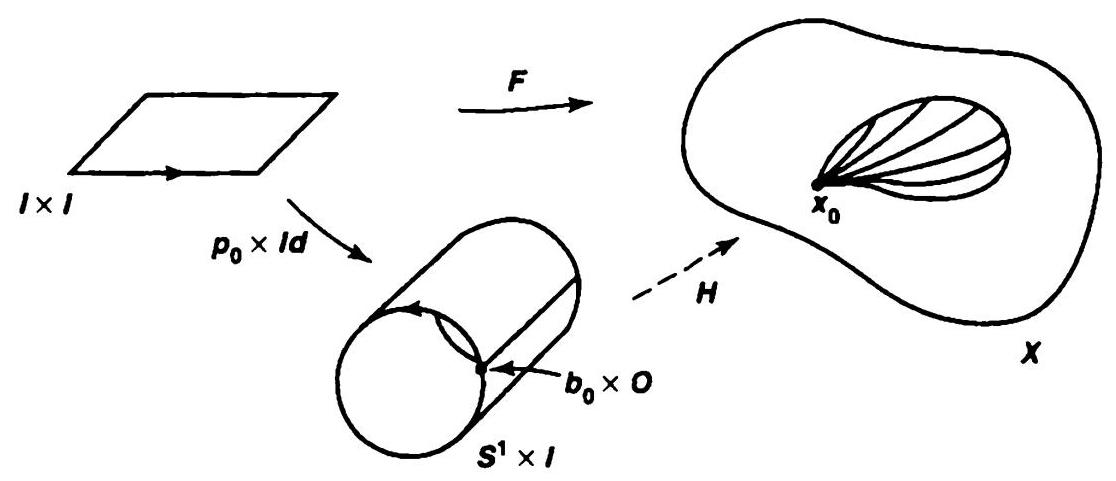
\includegraphics[width=1.0\textwidth]{images/55.2.jpg}
\end{center}
\hspace*{3em} 

Figure 55.2
\end{proof}
\begin{corollary}
	The inclusion map \(j \cdot  {S}^{1} \rightarrow  {\mathbb{R}}^{2} - 0\) is not nulhomotopic. The identity map \(i : {S}^{1} \rightarrow  {S}^{1}\) is not nulhomotopic.
\end{corollary}

\begin{proof}
	There is a retraction of \({\mathbb{R}}^{2} - 0\) onto \({S}^{1}\) given by the equation \(r( x)  = x/\parallel x\parallel\) . Therefore, \({j}_{ * }\) is injective, and hence nontrivial. Similarly, \({i}_{ * }\) is the identity homomorphism, and hence nontrivial.
\end{proof}
\begin{theorem}
	Given a nonvanishing \index{Vector field} on \({B}^{2}\) , there exists a point of \({S}^{1}\) where the \index{vector field@Vector field}vector field points directly inward and a point of \({S}^{1}\) where it points directly outward.
\end{theorem}

\begin{proof}
	A vector field on \({B}^{2}\) is an ordered pair \(( {x,v( x) })\) , where \(x\) is in \({B}^{2}\) and \(v\) is a continuous map of \({B}^{2}\) into \({\mathbb{R}}^{2}\) . In calculus, one often uses the notation
\[
\mathbf{v}( x)  = {v}_{1}( x) \mathbf{i} + {v}_{2}( x) \mathbf{j}
\]

for the function \(v\) , where \(\mathrm{i}\) and \(\mathrm{j}\) are the standard unit basis vectors in \({\mathbb{R}}^{2}\) . But we shall stick with simple functional notation. To say that a vector field is nonvanishing means that \(v( x)  \neq  \mathbf{0}\) for every \(x\) ; in such a case \(v\) actually maps \({B}^{2}\) into \({\mathbb{R}}^{2} - \mathbf{0}\) .

We suppose first that \(v( x)\) does not point directly inward at any point \(x\) of \({S}^{1}\) and derive a contradiction. Consider the map \(v : {B}^{2} \rightarrow  {\mathbb{R}}^{2} - \mathbf{0}\) ; let \(w\) be its restriction to \({S}^{1}\) . Because the map \(w\) extends to a map of \({B}^{2}\) into \({\mathbb{R}}^{2} - \mathbf{0}\) , it is nulhomotopic.

On the other hand, \(w\) is homotopic to the inclusion map \(j : {S}^{1} \rightarrow  {\mathbb{R}}^{2} - \mathbf{0}\) . Figure 55.3 illustrates the homotopy; one defines it formally by the equation

\[
F( {x,t})  = {tx} + ( {1 - t}) w( x) ,
\]

for \(x \in  {S}^{1}\) . We must show that \(F( {x,t})  \neq  \mathbf{0}\) . Clearly, \(F( {x,t})  \neq  \mathbf{0}\) for \(t = 0\) and \(t = 1\) . If \(F( {x,t})  = 0\) for some \(t\) with \(0 < t < 1\) , then \({tx} + ( {1 - t}) w( x)  = 0\) , so that \(w( x)\) equals a negative scalar multiple of \(x\) . But this means that \(w( x)\) points directly inward at \(x\) ! Hence \(F\) maps \({S}^{1} \times  I\) into \({\mathbb{R}}^{2} - \mathbf{0}\) , as desired.

It follows that \(j\) is nulhomotopic, contradicting the preceding corollary.

To show that \(v\) points directly outward at some point of \({S}^{1}\) , we apply the result just proved to the vector field \(( {x, - v( x) })\) .

\begin{center}
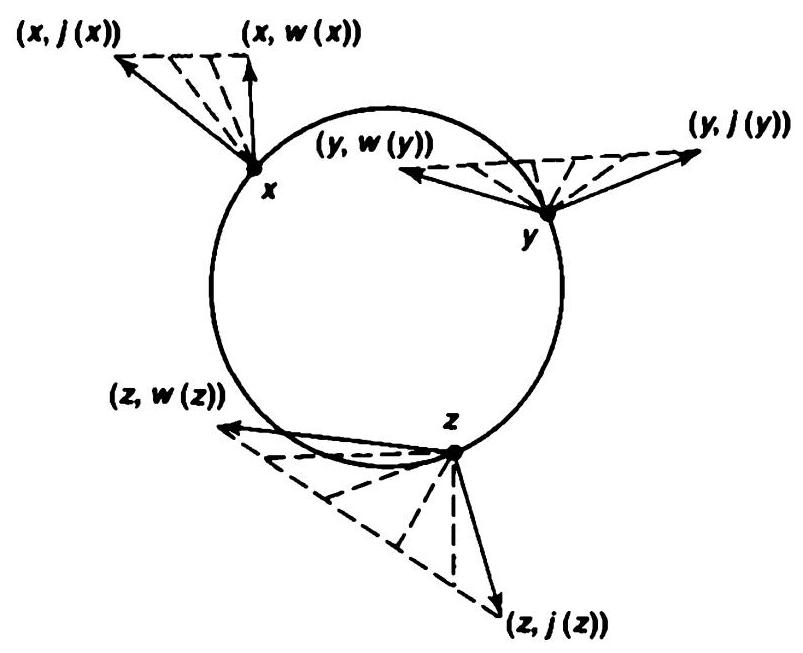
\includegraphics[width=0.7\textwidth]{images/55.3.jpg}
\end{center}
\hspace*{3em} 

Figure 55.3

We have already seen that every continuous map \(f : [  {0,1}]   \rightarrow  [  {0,1}]\) has a fixed point (see Exercise 3 of \(§{24}\) ). The same is true for the ball \({B}^{2}\) , although the proof is deeper:
\end{proof}
\begin{theorem}[\index{brouwer fixed-point theorem@Brouwer fixed-point theorem} for the disc]
	If \(f : {B}^{2} \rightarrow  {B}^{2}\) is continuous, then there exists a point \(x \in  {B}^{2}\) such that \(f( x)  = x\) .
\end{theorem}

\begin{proof}
	We proceed by contradiction. Suppose that \(f( x)  \neq  x\) for every \(x\) in \({B}^{2}\) . Then defining \(v( x)  = f( x)  - x\) gives us a nonvanishing vector field \(( {x,v( x) })\) on \({B}^{2}\) . But the vector field \(v\) cannot point directly outward at any point \(x\) of \({S}^{1}\) , for that would mean
\[
f( x)  - x = {ax}
\]

for some positive real number \(a\) , so that \(f( x)  = ( {1 + a}) x\) would lie outside the unit ball \({B}^{2}\) . We thus arrive at a contradiction.

One might well wonder why fixed-point theorems are of interest in mathematics. It turns out that many problems, such as problems concerning existence of solutions for systems of equations, for instance, can be formulated as fixed-point problems. Here is one example, a classical theorem of \index{frobenius theorem@Frobenius theorem} Frobenius. We assume some knowledge of linear algebra at this point.

*Corollary 55.7. Let \(A\) be a 3 by 3 matrix of positive real numbers. Then \(A\) has a positive real eigenvalue (characteristic value).

Proof. Let \(T : {\mathbb{R}}^{3} \rightarrow  {\mathbb{R}}^{3}\) be the linear transformation whose matrix (relative to the standard basis for \({\mathbb{R}}^{3}\) ) is \(A\) . Let \(B\) be the intersection of the 2 -sphere \({S}^{2}\) with the first octant

\[
\{  {( {{x}_{1},{x}_{2},{x}_{3}})  \mid  {x}_{1} \geq  0\text{ and }{x}_{2} \geq  0\text{ and }{x}_{3} \geq  0}\}
\]

of \({\mathbb{R}}^{3}\) . It is easy to show that \(B\) is homeomorphic to the ball \({B}^{2}\) , so that the fixed-point theorem holds for continuous maps of \(B\) into itself.

Now if \(x = ( {{x}_{1},{x}_{2},{x}_{3}})\) is in \(B\) , then all the components of \(x\) are nonnegative and at least one is positive. Because all entries of \(A\) are positive, the vector \(T( x)\) is a vector all of whose components are positive. As a result, the map \(x \rightarrow  T( x) /\parallel T( x) \parallel\) is a continuous map of \(B\) to itself, which therefore has a fixed point \({x}_{0}\) . Then

\[
T( {x}_{0})  = \begin{Vmatrix}{T( {x}_{0}) }\end{Vmatrix}{x}_{0},
\]

so that \(T\) (and therefore the matrix \(A\) ) has the positive real eigenvalue \(\begin{Vmatrix}{T( {x}_{0}) }\end{Vmatrix}\) .

Finally, we prove a theorem that implies that the triangular region

\[
T = \{ ( {x,y})  \mid  x \geq  0\text{ and }y \geq  0\text{ and }x + y \leq  1\}
\]

in \({\mathbb{R}}^{2}\) has topological dimension at least 2. (See \(§{50}\) .)

-Theorem 55.8. There is an \(\epsilon  > 0\) such that for every open covering \(\mathcal{A}\) of \(T\) by sets of diameter less than \(\epsilon\) , some point of \(T\) belongs to at least three elements of \(\mathcal{A}\) .

Proof. We use the fact that \(T\) is homeomorphic to \({B}^{2}\) , so that we can apply the results proved in this section to the space \(T\) .

Choose \(\epsilon  > 0\) so that no set of diameter less than \(\epsilon\) intersects all three edges of \(T\) . (In fact, \(\epsilon  = \frac{1}{2}\) will do.) We suppose that \(\mathcal{A} = \{  {{U}_{1},\ldots ,{U}_{n}}\}\) is an open covering of \(T\) by sets of diameter less than \(\epsilon\) , such that no three elements of \(\mathcal{A}\) intersect, and derive a contradiction.

For each \(i = 1,\ldots ,n\) , choose a vertex \({v}_{i}\) of \(T\) as follows: If \({U}_{i}\) intersects two edges of \(T\) , let \({v}_{i}\) be the vertex common to these edges. If \({U}_{i}\) intersects only one edge of \(T\) , let \({v}_{i}\) be one of the end points of this edge. If \({U}_{i}\) intersects no edge of \(T\) , let \({v}_{i}\) be any vertex of \(T\) .

Now let \(\{  {\phi }_{i}\}\) be a partition of unity dominated by \(\{  {{U}_{1},\ldots ,{U}_{n}}\}\) . (See \(§{36}\) .) Define \(k : T \rightarrow  {\mathbb{R}}^{2}\) by the equation

\[
k( x)  = \mathop{\sum }\limits_{{i = 1}}^{n}{\phi }_{i}( x) {v}_{i}
\]

Then \(k\) is continuous. Given a point \(x\) of \(T\) , it lies in at most two elements of \(\mathcal{A}\) ; hence at most two of the numbers \({\phi }_{i}( x)\) are nonzero. Then \(k( x)  = {v}_{i}\) if \(x\) lies in only one open set \({U}_{i}\) , and \(k( x)  = t{v}_{i} + ( {1 - t}) {v}_{j}\) for some \(t\) with \(0 \leq  t \leq  1\) if \(x\) lies in two open sets \({U}_{i}\) and \({U}_{j}\) . In either case, \(k( x)\) belongs to the union of the edges of \(T\) , which is Bd \(T\) . Thus \(k\) maps \(T\) into Bd \(T\) .

Furthermore, \(k\) maps each edge of \(T\) into itself. For if \(x\) belongs to the edge \({vw}\) of \(T\) , any open set \({U}_{i}\) containing \(x\) intersects this edge, so that \({v}_{i}\) must equal either \(v\) or \(w\) . The definition of \(k\) then shows that \(k( x)\) belongs to \({vw}\) .

Let \(h : \operatorname{Bd}T \rightarrow  \operatorname{Bd}T\) be the restriction of \(k\) to \(\operatorname{Bd}T\) . Since \(h\) can be extended to the continuous map \(k\) , it is nulhomotopic. On the other hand, \(h\) is homotopic to the identity map of \(\operatorname{Bd}T\) to itself; indeed, since \(h\) maps each edge of \(T\) into itself, the straight-line homotopy between \(h\) and the identity map of \(\operatorname{Bd}T\) is such a homotopy. But the identity map \(i\) of \(\operatorname{Bd}T\) is not nulhomotopic.
\end{proof}
\section*{Exercises}
\begin{enumerate}[itemsep=0.4em, parsep=0pt, topsep=0pt, partopsep=0pt, leftmargin=*, label=\arabic*., ref=\arabic*]
\item Show that if \(A\) is a retract of \({B}^{2}\) , then every continuous map \(f : A \rightarrow  A\) has a fixed point.
\item Show that if \(h : {S}^{1} \rightarrow  {S}^{1}\) is nulhomotopic, then \(h\) has a fixed point and \(h\) maps some point \(x\) to its \index{antipode@Antipode}antipode \(- x\)
\item Show that if \(A\) is a nonsingular 3 by 3 matrix having nonnegative entries, then \(A\) has a positive real eigenvalue.
\item Suppose that you are given the fact that for each \(n\) , there is no \index{retraction@Retraction}retraction \(r\) : \({B}^{n + 1} \rightarrow  {S}^{n}\) . (This result can be proved using more advanced techniques of algebraic topology.) Prove the following:
  \begin{enumerate}[itemsep=0.2em, parsep=0pt, topsep=0pt, partopsep=0pt, leftmargin=*, label=(\alph*), align=left]
  \item The identity map \(i : {S}^{n} \rightarrow  {S}^{n}\) is not nulhomotopic.
  \item The inclusion map \(j : {S}^{n} \rightarrow  {\mathbb{R}}^{n + 1} - \mathbf{0}\) is not nulhomotopic.
  \item Every nonvanishing vector field on \({B}^{n + 1}\) points directly outward at some point of \({S}^{n}\) , and directly inward at some point of \({S}^{n}\) .
  \item Every continuous map \(f : {B}^{n + 1} \rightarrow  {B}^{n + 1}\) has a fixed point.
  \item Every \(n + 1\) by \(n + 1\) matrix with positive real entries has a positive eigenvalue.
  \item If \(h : {S}^{n} \rightarrow  {S}^{n}\) is nulhomotopic, then \(h\) has a fixed point and \(h\) maps some point \(x\) to its antipode \(- x\) .
  \end{enumerate}
\end{enumerate}
\section*{*§ 56 The Fundamental Theorem of Algebra}

It is a basic fact about the complex numbers that every polynomial equation

\[
{x}^{n} + {a}_{n - 1}{x}^{n - 1} + \cdots  + {a}_{1}x + {a}_{0} = 0
\]

of \index{degree of a map@Degree of a map} degree \(n\) with real or complex coefficients has \(n\) roots (if the roots are counted according to their multiplicities). You probably first were told this fact in high school algebra, although it is doubtful that it was proved for you at that time.

The proof is, in fact, rather hard; the most difficult part is to prove that every polynomial equation of positive degree has at least one root. There are various ways of doing this. One can use only techniques of algebra; this proof is long and arduous. Or one can develop the theory of analytic functions of a complex variable to the point where it becomes a trivial corollary of Liouville's theorem. Or one can prove it as a relatively easy corollary of our computation of the fundamental group of the circle; this we do now.

\begin{theorem}[The fundamental theorem of algebra]
	A polynomial equation

\[
{x}^{n} + {a}_{n - 1}{x}^{n - 1} + \cdots  + {a}_{1}x + {a}_{0} = 0
\]

of degree \(n > 0\) with real or complex coefficients has at least one (real or complex) root.
\end{theorem}

\begin{proof}
	Step 1. Consider the map \(f : {S}^{1} \rightarrow  {S}^{1}\) given by \(f( z)  = {z}^{n}\) , where \(z\) is a complex number. We show that the induced homomorphism \({f}_{ * }\) of fundamental groups is injective.
Let \({p}_{0} : I \rightarrow  {S}^{1}\) be the standard loop in \({S}^{1}\) ,

\[
{p}_{0}( s)  = {e}^{2\pi is} = ( {\cos {2\pi s},\sin {2\pi s}}) .
\]

Its image under \({f}_{ * }\) is the loop

\[
f( {{p}_{0}( s) })  = {( {e}^{2\pi is}) }^{n} = ( {\cos {2\pi ns},\sin {2\pi ns}}) .
\]

This loop lifts to the path \(s \rightarrow  {ns}\) in the covering space \(\mathbb{R}\) . Therefore, the loop \(f \circ  {p}_{0}\) corresponds to the integer \(n\) under the standard isomorphism of \({\pi }_{1}( {{S}^{1},{b}_{0}})\) with the integers, whereas \({p}_{0}\) corresponds to the number 1 . Thus \({f}_{ * }\) is ``multiplication by \(n\) `` in the fundamental group of \({S}^{1}\) , so that in particular, \({f}_{ * }\) is injective.

Step 2. We show that if \(g : {S}^{1} \rightarrow  {\mathbb{R}}^{2} - \mathbf{0}\) is the map \(g( z)  = {z}^{n}\) , then \(g\) is not nulhomotopic.

The map \(g\) equals the map \(f\) of Step 1 followed by the inclusion map \(j : {S}^{1} \rightarrow\)  \({\mathbb{R}}^{2} - \mathbf{0}\) . Now \({f}_{ * }\) is injective, and \({j}_{ * }\) is injective because \({S}^{1}\) is a retract of \({\mathbb{R}}^{2} - \mathbf{0}\) . Therefore, \({g}_{ * } = {j}_{ * } \circ  {f}_{ * }\) is injective. Thus \(g\) cannot be nulhomotopic.

Step 3. Now we prove a special case of the theorem. Given a polynomial equation

\[
{x}^{n} + {a}_{n - 1}{x}^{n - 1} + \cdots  + {a}_{1}x + {a}_{0} = 0,
\]

we assume that

\[
| {a}_{n - 1}|  + \cdots  + | {a}_{1}|  + | {a}_{0}|  < 1
\]

and show that the equation has a root lying in the unit ball \({B}^{2}\) .

Assume it has no such root. Then we can define a map \(k : {B}^{2} \rightarrow  {\mathbb{R}}^{2} - \mathbf{0}\) by the equation

\[
k( z)  = {z}^{n} + {a}_{n - 1}{z}^{n - 1} + \cdots  + {a}_{1}z + {a}_{0}.
\]

Let \(h\) be the restriction of \(k\) to \({S}^{1}\) . Because \(h\) extends to a map of the unit ball into \({\mathbb{R}}^{2} - 0\) , the map \(h\) is nulhomotopic.

On the other hand, we shall define a homotopy \(F\) between \(h\) and the map \(g\) of Step 2: since \(g\) is not nulhomotopic, we have a contradiction. We define \(F : {S}^{1} \times  I \rightarrow\)  \({\mathbb{R}}^{2} - 0\) by the equation

\[
F( {z,t})  = {z}^{n} + t( {{a}_{n - 1}{z}^{n - 1} + \cdots  + {a}_{0}}) .
\]

See Figure 56.1; \(F( {z,t})\) never equals 0 because

\[
| {F( {z,t}) }|  \geq  | {z}^{n}|  - | {t( {{a}_{n - 1}{z}^{n - 1} + \cdots  + {a}_{0}}) }|
\]

\[
\geq  1 - t( {| {{a}_{n - 1}{z}^{n - 1}}|  + \cdots  + | {a}_{0}| })
\]

\[
= 1 - t( {| {a}_{n - 1}|  + \cdots  + | {a}_{0}| })  > 0\text{ . }
\]

\begin{center}
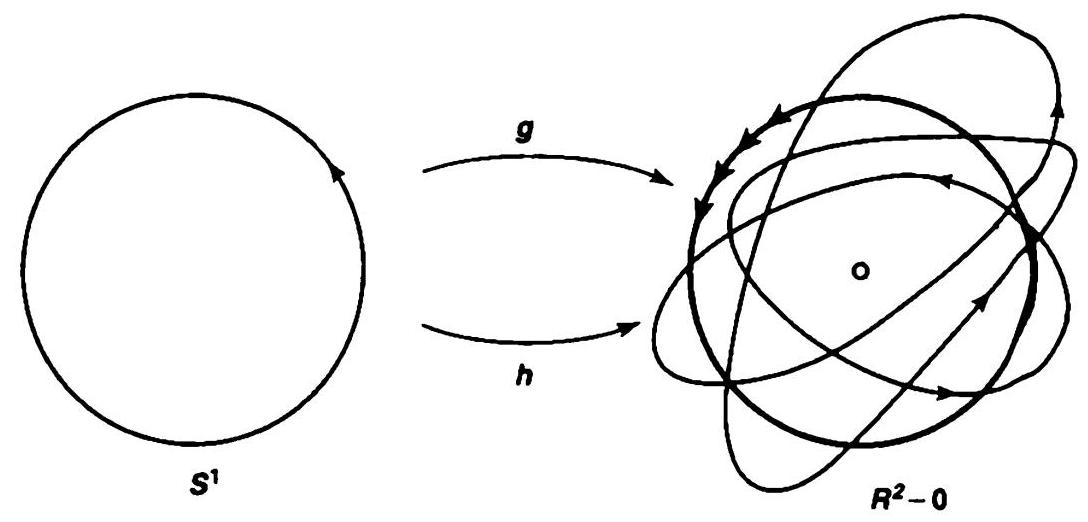
\includegraphics[width=1.0\textwidth]{images/56.1.jpg}
\end{center}
\hspace*{3em} 

Figure 56.1

Step 4. Now we prove the general case. Given a polynomial equation

\[
{x}^{n} + {a}_{n - 1}{x}^{n - 1} + \cdots  + {a}_{1}x + {a}_{0} = 0,
\]

let us choose a real number \(c > 0\) and substitute \(x = {cy}\) . We obtain the equation

\[
{( cy) }^{n} + {a}_{n - 1}{( cy) }^{n - 1} + \cdots  + {a}_{1}( {cy})  + {a}_{0} = 0
\]

or

\[
{y}^{n} + \frac{{a}_{n - 1}}{c}{y}^{n - 1} + \cdots  + \frac{{a}_{1}}{{c}^{n - 1}}y + \frac{{a}_{0}}{{c}^{n}} = 0.
\]

If this equation has the root \(y = {y}_{0}\) , then the original equation has the root \({x}_{0} = c{y}_{0}\) . So we need merely choose \(c\) large enough that

\[
| \frac{{a}_{n - 1}}{c}|  + | \frac{{a}_{n - 2}}{{c}^{2}}|  + \cdots  + | \frac{{a}_{1}}{{c}^{n - 1}}|  + | \frac{{a}_{0}}{{c}^{n}}|  < 1
\]

to reduce the theorem to the special case considered in Step 3.
\end{proof}
\section*{Exercises}
\begin{enumerate}[itemsep=0.4em, parsep=0pt, topsep=0pt, partopsep=0pt, leftmargin=*, label=\arabic*., ref=\arabic*]
\item Given a polynomial equation \[ {x}^{n} + {a}_{n - 1}{x}^{n - 1} + \cdots  + {a}_{1}x + {a}_{0} = 0 \] with real or complex coefficients. Show that if \(| {a}_{n - 1}|  + \cdots  + | {a}_{1}|  + | {a}_{0}|  < 1\) , then all the roots of the equation lie interior to the unit ball \({B}^{2}\) . [Hint: Let \(g( x)  = 1 + {a}_{n - 1}x + \cdots  + {a}_{1}{x}^{n - 1} + {a}_{0}{x}^{n}\) , and show that \(g( x)  \neq  0\) for \(x \in  {B}^{2}\) .]
\item Find a circle about the origin containing all the roots of the polynomial equation \({x}^{7} + {x}^{2} + 1 = 0.\)
\end{enumerate}
\section*{*§ 57 The Borsuk-Ulam Theorem}

\index{borsuk-ulam theorem@Borsuk-Ulam Theorem} Here is a ``brain-teaser'' problem: Suppose you are given a bounded polygonal region \(A\) in the plane \({\mathbb{R}}^{2}\) . No matter what shape \(A\) has, it is easy to show that there exists a straight line that bisects \(A\) , that is, one that cuts the area of \(A\) in half. Simply take the horizontal line \(y = c\) , let \(f( c)\) denote the area of that part of \(A\) that lies beneath this line, note that \(f\) is a continuous function of \(c\) , and use the intermediate-value theorem to find a value of \(c\) for which \(f( c)\) equals exactly half the area of \(A\) .

But now suppose instead that you are given two such regions \({A}_{1}\) and \({A}_{2}\) , you are asked to find a single line that bisects them both. It is not obvious even that there exists such a line. Try to find one for an arbitrary pair \index{Topological dimension!of triangular region}of triangular regions if you have doubts!

In fact, such a line always exists This result is a corollary of a well-known theorem called the \index{borsuk-ulam theorem@Borsuk-Ulam theorem}Borsuk-Ulam theorem, to which we now turn.

\begin{definition}
	If \(x\) is a point of \({S}^{n}\) , then its antipode is the point \(- x\) . A map \(h : {S}^{n} \rightarrow\)  \({S}^{m}\) is said to be \index{antipode-preserving@Antipode-preserving}antipode-preserving if \(h( {-x})  =  - h( x)\) for all \(x \in  {S}^{n}\) .
\end{definition}

\begin{theorem}
	If \(h : {S}^{1} \rightarrow  {S}^{1}\) is continuous and antipode-preserving, then \(h\) is not nulhomotopic.
\end{theorem}

\begin{proof}
	Let \({b}_{0}\) be the point(1,0)of \({S}^{1}\) . Let \(\rho  : {S}^{1} \rightarrow  {S}^{1}\) be a rotation of \({S}^{1}\) that maps \(h( {b}_{0})\) to \({b}_{0}\) . Since \(\rho\) preserves antipodes, so does the composite \(\rho  \circ  h\) . Furthermore, if \(H\) were a homotopy between \(h\) and a constant map, then \(\rho  \circ  H\) would be a homotopy between \(\rho  \circ  h\) and a constant map. Therefore, it suffices to prove the theorem under the additional hypothesis that \(h( {b}_{0})  = {b}_{0}\) .
Step 1. Let \(q : {S}^{1} \rightarrow  {S}^{1}\) be the map \(q( z)  = {z}^{2}\) , where \(z\) is a complex number. Or in real coordinates, \(q( {\cos \theta ,\sin \theta })  = ( {\cos {2\theta },\sin {2\theta }})\) . The map \(q\) is a quotient map, being continuous, closed, and surjective. The inverse image under \(q\) of any point of \({S}^{1}\) consists of two antipodal points \(z\) and \(- z\) of \({S}^{1}\) . Because \(h( {-z})  =  - h( z)\) , one has the equation \(q( {h( {-z}) })  = q( {h( z) })\) . Therefore, because \(q\) is a quotient map, the map \(q \circ  h\) induces a continuous map \(k : {S}^{1} \rightarrow  {S}^{1}\) such that \(k \circ  q = q \circ  h\) . Note that \(q( {b}_{0})  = h( {b}_{0})  = {b}_{0}\) , so that \(k( {b}_{0})  = {b}_{0}\) as well. Also, \(h( {-{b}_{0}})  =  - {b}_{0}\) . Step 2. We show that the homomorphism \({k}_{ * }\) of \({\pi }_{1}( {{S}^{1},{b}_{0}})\) with itself is nontrivial. For this purpose, we first show that \(q\) is a covering map. (We gave this as an exercise in \(§{53}\) .) The proof is similar to the proof that the standard map \(p : \mathbb{R} \rightarrow  {S}^{1}\) is a covering map. If, for instance, \(U\) is the subset of \({S}^{1}\) consisting of those points having positive second coordinate, then \({p}^{-1}( U)\) consist of those points of \({S}^{1}\) lying in the first and third quadrants of \({\mathbb{R}}^{2}\) . The map \(q\) carries each of these sets homeomorphically onto \(U\) . Similar arguments apply when \(U\) is the intersection of \({S}^{1}\) with the open lower half-plane, or with the open right and left half-planes.

\begin{center}
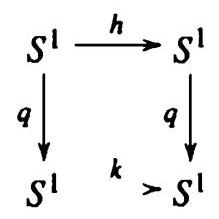
\includegraphics[width=0.2\textwidth]{images/57.0.jpg}
\end{center}
\hspace*{3em} 

Second, we note that if \(\widetilde{f}\) is any path in \({S}^{1}\) from \({b}_{0}\) to \(- {b}_{0}\) , then the loop \(f = q \circ  \widetilde{f}\) represents a nontrivial element of \({\pi }_{1}( {{S}^{1},{b}_{0}})\) . For \(\widetilde{f}\) is a lifting of \(f\) to \({S}^{1}\) that begins at \({b}_{0}\) and does not end at \({b}_{0}\) .

Finally, we show \({k}_{ * }\) is nontrivial. Let \(\widetilde{f}\) be a path in \({S}^{1}\) from \({b}_{0}\) to \(- {b}_{0}\) , and let \(f\) be the loop \(q \circ  \bar{f}\) . Then \({k}_{ * }[  f]\) is not trivial, for \({k}_{ * }[  f]   = [  {k \circ  ( {q \circ  \widetilde{f}}) }]   = [  {q \circ  ( {h \circ  \bar{f}}) }]\) ; the latter is nontrivial because \(h \circ  \bar{f}\) is a path in \({S}^{1}\) from \({b}_{0}\) to \(- {b}_{0}\) .

Step 3. Finally, we show that the homomorphism \({h}_{ * }\) is nontrivial, so that \(h\) cannot be nulhomotopic.

The homomorphism \({k}_{ * }\) is injective, being a nontrivial homomorphism of an infinite cyclic group with itself. The homomorphism \({q}_{ * }\) is also injective; indeed, \({q}_{ * }\) corresponds to multiplication by two in the group of integers. It follows that \({k}_{ * } \circ  {q}_{ * }\) is injective. Since \({q}_{ * } \circ  {h}_{ * } = {k}_{ * } \circ  {q}_{ * }\) , the homomorphism \({h}_{ * }\) must be injective as well.

\begin{center}
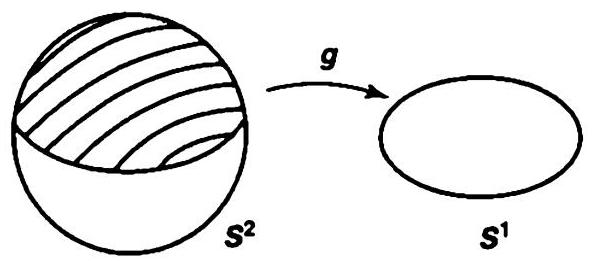
\includegraphics[width=0.5\textwidth]{images/57.1.jpg}
\end{center}
\hspace*{3em} 

Figure 57.1
\end{proof}
\begin{theorem}
	There is no continuous antipode-preserving map \(g : {S}^{2} \rightarrow  {S}^{1}\) .
\end{theorem}

\begin{proof}
	Suppose \(g : {S}^{2} \rightarrow  {S}^{1}\) is continuous and antipode preserving. Let us take \({S}^{1}\) to be the equator of \({S}^{2}\) . Then the restriction of \(g\) to \({S}^{1}\) is a continuous antipode-preserving map \(h\) of \({S}^{1}\) to itself. By the preceding theorem, \(h\) is not nulhomotopic. But the upper hemisphere \(E\) of \({S}^{2}\) is homeomorphic to the ball \({B}^{2}\) , and \(g\) is a continuous extension of \(h\) to \(E\) ! See Figure 57.1.
\end{proof}
\begin{theorem}[Borsuk-Ulam theorem for \({S}^{2}\)]
	Given a continuous map \(f : {S}^{2} \rightarrow\)  \({\mathbb{R}}^{2}\) , there is a point \(x\) of \({S}^{2}\) such that \(f( x)  = f( {-x})\) .
\end{theorem}

\begin{proof}
	Suppose that \(f( x)  \neq  f( {-x})\) for all \(x \in  {S}^{2}\) . Then the map
\[
g( x)  = [  {f( x)  - f( {-x}) }]  /\parallel f( x)  - f( {-x}) \parallel
\]

is a continuous map \(g : {S}^{2} \rightarrow  {S}^{1}\) such that \(g( {-x})  =  - g( x)\) for all \(x\) .
\end{proof}
\begin{theorem}[The \index{Bisection theorem}]
	Given two bounded polygonal regions in \({\mathbb{R}}^{2}\) , there exists a line in \({\mathbb{R}}^{2}\) that bisects each of them.
\end{theorem}

\begin{proof}
	We take two bounded polygonal regions \({A}_{1}\) and \({A}_{2}\) in the plane \({\mathbb{R}}^{2} \times  1\) in \({\mathbb{R}}^{3}\) , and show there is a line \(L\) in this plane that bisects each of them.
Given a point \(u\) of \({S}^{2}\) , let us consider the plane \(P\) in \({\mathbb{R}}^{3}\) passing through the origin that has \(u\) as its unit normal vector. This plane divides \({\mathbb{R}}^{3}\) into two half-spaces; let \({f}_{i}( u)\) equal the area of that portion of \({A}_{i}\) that lies on the same side of \(P\) as does the vector \(u\) .

If \(u\) is the unit vector \(\mathbf{k}\) , then \({f}_{i}( u)  = \operatorname{area}{A}_{i}\) ; and if \(u =  - \mathbf{k}\) , then \({f}_{i}( u)  = 0\) . Otherwise, the plane \(P\) intersects the plane \({\mathbb{R}}^{2} \times  1\) in a line \(L\) that splits \({\mathbb{R}}^{2} \times  1\) into two half-planes, and \({f}_{i}( u)\) is the area of that part of \({A}_{i}\) that lies on one side of this line. See Figure 57.2.

\begin{center}
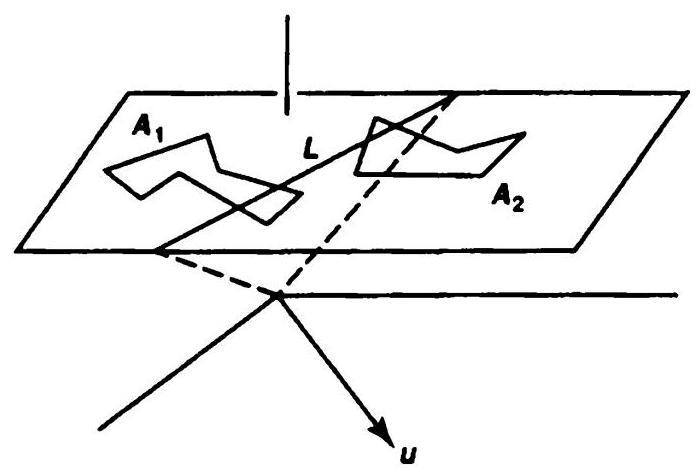
\includegraphics[width=0.6\textwidth]{images/57.2.jpg}
\end{center}
\hspace*{3em} 

Figure 57.2

Replacing \(u\) by \(- u\) gives us the same plane \(P\) , but the other half-space, so that \({f}_{i}( {-u})\) is the area of that part of \({A}_{i}\) that lies on the other side of \(P\) from \(u\) . It follows that

\[
{f}_{i}( u)  + {f}_{i}( {-u})  = \operatorname{area}{A}_{i}.
\]

Now consider the map \(F : {S}^{2} \rightarrow  {\mathbb{R}}^{2}\) given by \(F( u)  = ( {{f}_{1}( u) ,{f}_{2}( u) })\) . The Borsuk-Ulam theorem gives us a point \(u\) of \({S}^{2}\) for which \(F( u)  = F( {-u})\) . Then \({f}_{i}( u)  = {f}_{i}( {-u})\) for \(i = 1,2\) , that \({f}_{i}( u)  = \frac{1}{2}\) area \({A}_{i}\) , as desired.

We have proved the \index{bisection theorem@Bisection theorem}bisection theorem for bounded polygonal regions in the plane. However, all that was needed in the proof was the existence of an additive area function for \({A}_{1}\) and \({A}_{2}\) . Thus, the theorem holds for any two sets \({A}_{1}\) and \({A}_{2}\) that are ``Jordan-measurable'' in the sense used in analysis.

These theorems generalize to higher dimensions, but the proofs are considerably more sophisticated. The generalized version of the bisection theorem states that given \(n\) Jordan-measurable sets in \({\mathbb{R}}^{n}\) , there exists a plane of dimension \(n - 1\) that bisects them all. In the case \(n = 3\) , this result goes by the pleasant name of the ``\index{Ham sandwich theorem}.'' If one considers a ham sandwich to consist of two pieces of bread and a slab of ham, then the bisection theorem says that one can divide each of them precisely in half with a single whack of a cleaver \({}^{1}\)
\end{proof}
\section*{Exercises}
\begin{enumerate}[itemsep=0.4em, parsep=0pt, topsep=0pt, partopsep=0pt, leftmargin=*, label=\arabic*., ref=\arabic*]
\item Prove the following ``theorem of meteorology'': At any given moment in time, there exists a pair of antipodal points on the surface of the earth at which both the temperature and the barometric pressure are equal.
\item Show that if \(g : {S}^{2} \rightarrow  {S}^{2}\) is continuous and \(g( x)  \neq  g( {-x})\) for all \(x\) , then \(g\) is surjective. [Hint: If \(p \in  {S}^{2}\) , then \({S}^{2} - \{ p\}\) is homeomorphic to \({\mathbb{R}}^{2}\) .]
\item Let \(h : {S}^{1} \rightarrow  {S}^{1}\) be continuous and antipode-preserving with \(h( {b}_{0})  = {b}_{0}\) . Show that \({h}_{ * }\) carries a generator of \({\pi }_{1}( {{S}^{1},{b}_{0}})\) to an odd power of itself. [Hint: If \(k\) is the map constructed in the proof of Theorem 57.1, show that \({k}_{ * }\) does the same.]
\item Suppose you are given the fact that for each \(n\) , no continuous antipode-preserving map \(h : {S}^{n} \rightarrow  {S}^{n}\) is nulhomotopic. (This result can be proved using more advanced techniques of algebraic topology.) Prove the following:
  \begin{enumerate}[itemsep=0.2em, parsep=0pt, topsep=0pt, partopsep=0pt, leftmargin=*, label=(\alph*), align=left]
  \item There is no retraction \(r : {B}^{n + 1} \rightarrow  {S}^{n}\) .
  \item There is no continuous antipode-preserving map \(g : {S}^{n + 1} \rightarrow  {S}^{n}\) .
  \item (Borsuk-Ulam theorem) Given a continuous map \(f : {S}^{n + 1} \rightarrow  {\mathbb{R}}^{n + 1}\) , there is a point \(x\) of \({S}^{n + 1}\) such that \(f( x)  = f( {-x})\) .
  \item If \({A}_{1},\ldots ,{A}_{n + 1}\) are bounded measurable sets in \({\mathbb{R}}^{n + 1}\) , there exists an \(n\) - plane in \({\mathbb{R}}^{n + 1}\) that bisects each of them.
  \end{enumerate}
\end{enumerate}
\section*{§ 58 Deformation Retracts and Homotopy Type}

\index{deformation retract@Deformation Retract} As we have seen, one way of obtaining information about the fundamental group of a space \(X\) is to study the covering spaces of \(X\) . Another is one we discuss in this section, which involves the notion of \index{Homotopy type}. It provides a method for reducing the problem of computing the fundamental group of a space to that of computing the fundamental group of some other space-preferably, one that is more familiar.

We begin with a lemma.

\begin{lemma}
	Let \(h,k.( {X,{x}_{0}})  \rightarrow  ( {Y,{y}_{0}})\) be continuous maps. If \(h\) and \(k\) are homotopic, and if the image of the base point \({x}_{0}\) of \(X\) remains fixed at \({y}_{0}\) during the homotopy, then the homomorphisms \({h}_{ * }\) and \({k}_{ * }\) are equal.
\end{lemma}

\begin{proof}
	The proof is immediate. By assumption, there is a homotopy \(H : X \times  I \rightarrow  Y\) between \(h\) and \(k\) such that \(H( {{x}_{0},t})  = {y}_{0}\) for all \(t\) . It follows that if \(f\) is a loop in \(X\) based at \({x}_{0}\) , then the composite
\[
I \times  I\xrightarrow[]{f \times  \mathrm{{id}}}X \times  I\xrightarrow[]{H}Y
\]

is a homotopy between \(h \circ  f\) and \(k \circ  f\) ; it is a path homotopy because \(f\) is a loop at \({x}_{0}\) and \(H\) maps \({x}_{0} \times  l\) to \({y}_{0}\) .

Using this lemma, we generalize a result about the space \({\mathbb{R}}^{2} - \mathbf{0}\) proved earlier, proving that the homomorphism induced by inclusion \(j : {S}^{1} \rightarrow  {\mathbb{R}}^{2} - \mathbf{0}\) is not only injective but surjective as well. More generally, we prove the following:
\end{proof}
\begin{theorem}
	The inclusion map \(j : {S}^{n} \rightarrow  {\mathbb{R}}^{n + 1} - \mathbf{0}\) induces an isomorphism of fundamental groups.
\end{theorem}

\begin{proof}
	Let \(X = {\mathbb{R}}^{n + 1} - \mathbf{0}\) ; let \({b}_{0} = ( {1,0,\ldots ,0})\) . Let \(r : X \rightarrow  {S}^{n}\) be the map \(r( x)  = x/\parallel x\parallel\) . Then \(r \circ  j\) is the identity map of \({S}^{n}\) , so that \({r}_{ * } \circ  {j}_{ * }\) is the identity homomorphism of \({\pi }_{1}( {{S}^{n},{b}_{0}})\) .
Now consider the composite \(j \circ  r\) , which maps \(X\) to itself;

\[
X\overset{r}{ \rightarrow  }{S}^{n}\overset{j}{ \rightarrow  }X
\]

This map is not the identity map of \(X\) , but it is homotopic to the identity map. Indeed, the straight-line homotopy \(H : X \times  I \rightarrow  X\) , given by

\[
H( {x,t})  = ( {1 - t}) x + {tx}/\parallel x\parallel ,
\]

is a homotopy between the identity map of \(X\) and the map \(j \circ  r\) . For \(H( {x,t})\) is never equal to0, because \(( {1 - t})  + t/\parallel x\parallel\) is a number between 1 and \(1/\parallel x\parallel\) . Note that the point \({b}_{0}\) remains fixed during the homotopy, since \(\begin{Vmatrix}{b}_{0}\end{Vmatrix} = 1\) . It follows from the preceding lemma that the homomorphism \({( j \circ  r) }_{ * } = {j}_{ * } \circ  {r}_{ * }\) is the identity homomorphism of \({\pi }_{1}( {X,{b}_{0}})\) .

What made the preceding proof work? Roughly speaking, it worked because we had a natural way of deforming the identity map of \({\mathbb{R}}^{n + 1} - 0\) to a map that collapsed all of \({\mathbb{R}}^{n + 1} - \mathbf{0}\) onto \({S}^{n}\) . The deformation \(H\) gradually collapsed each radial line emanating from the origin to the point where it intersected \({S}^{n}\) ; each point of \({S}^{n}\) remained fixed during this deformation.

Figure 58.1 illustrates, in the case \(n = 1\) , how the deformation \(H\) gives rise to a path homotopy \(H( {f( s) ,t})\) between the loop \(f\) in \({\mathbb{R}}^{2} - \mathbf{0}\) and the loop \(g = f/\parallel f\parallel\) in \({S}^{1}\) .

% \begin{center}
% 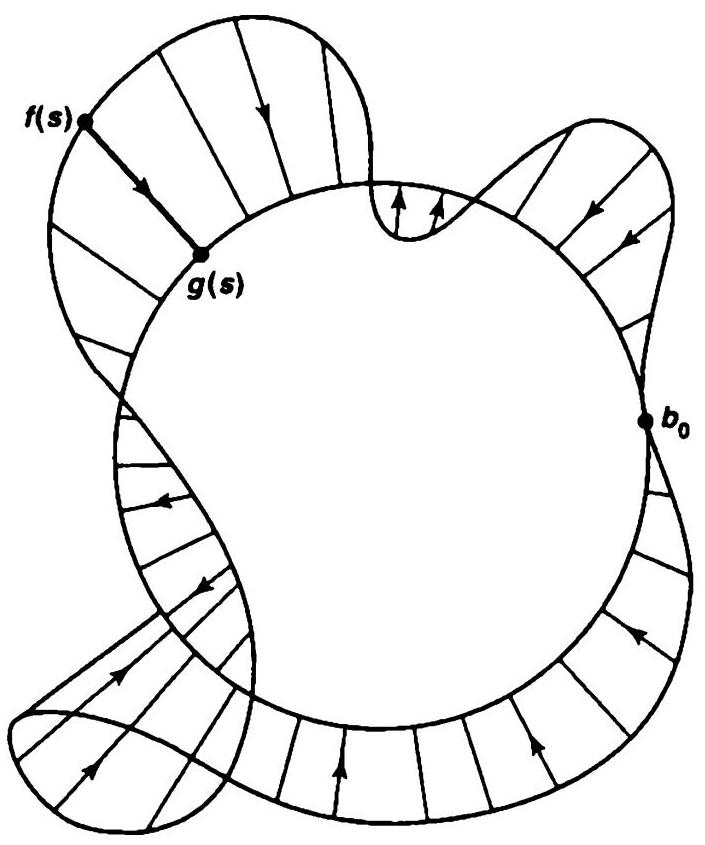
\includegraphics[width=0.6\textwidth]{images/58.1.jpg}
% \end{center}
\hspace*{3em} 

Figure 58.1

These comments lead us to formulate a more general situation in which the same procedure applies.
\end{proof}
\begin{definition}
	Let \(A\) be a subspace of \(X\) . We say that \(A\) is a deformation retract of \(X\) if the identity map of \(X\) is homotopic to a map that carries all of \(X\) into \(A\) , such that each point of \(A\) remains fixed during the homotopy. This means that there is a continuous map \(H : X \times  I \rightarrow  X\) such that \(H( {x,0})  = x\) and \(H( {x,1})  \in  A\) for all \(x \in  X\) , and \(H( {a,t})  = a\) for all \(a \in  A\) . The homotopy \(H\) is called a \index{Deformation retraction} of \(X\) onto \(A\) . The map \(r : X \rightarrow  A\) defined by the equation \(r( x)  = H( {x,1})\) is a retraction of \(X\) onto \(A\) , and \(H\) is a homotopy between the identity map of \(X\) and the map \(j \circ  r\) , where \(j : A \rightarrow  X\) is inclusion.
\end{definition}

The proof of the preceding theorem generalizes immediately to prove the following:

\begin{theorem}
	Let \(A\) be a deformation retract of \(X\) ; let \({x}_{0} \in  A\) . Then the inclusion map

\[
j : ( {A,{x}_{0}})  \rightarrow  ( {X,{x}_{0}})
\]

induces an isomorphism of fundamental groups.
\end{theorem}

\end{example}
\end{centeredblock}

\begin{centeredblock}
\begin{example}
	Let \(B\) denote the \(z\) -axis in \({\mathbb{R}}^{3}\) Consider the space \({\mathbb{R}}^{3} - B\) It has the punctured \({xy}\) -plane \(( {{\mathbb{R}}^{2} - 0})  \times  0\) as a \index{deformation retract@Deformation retract}deformation retract The map \(H\) defined by the equation

\[
H( {x,y,z,t})  = ( {x,y,( {1 - t}) z})
\]

is a \index{deformation retraction@Deformation retraction}deformation retraction; it gradually collapses each line parallel to the \(z\) -axis into the point where the line intersects the \({xy}\) -plane. We conclude that the space \({\mathbb{R}}^{3} - B\) has an infinite cyclic fundamental group.

\end{example}
\end{centeredblock}

\begin{centeredblock}
\begin{example}
	Consider \({\mathbb{R}}^{2} - p - q\) , the \index{Doubly punctured plane}. We assert it has the ``figure eight'' space as a deformation retract. Rather than writing equations, we merely sketch the deformation retraction; it is the three-stage deformation indicated in Figure 58.2.

\begin{center}
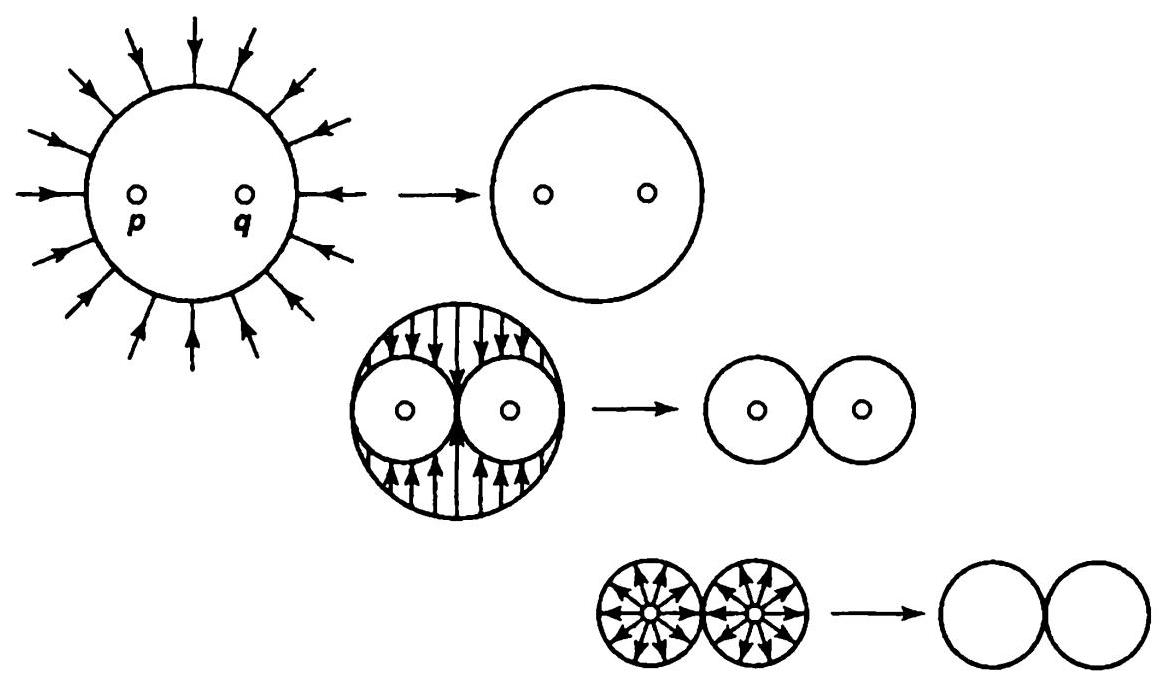
\includegraphics[width=1.0\textwidth]{images/58.2.jpg}
\end{center}
\hspace*{3em} 

Figure 58.2

\end{example}
\end{centeredblock}

\begin{centeredblock}
\begin{example}
	Another deformation retract of \({\mathbb{R}}^{2} - p - q\) is the ``\index{Theta space}''

\[
\theta  = {S}^{1} \cup  ( {0 \times  [  {-1,1}]  })
\]

we leave it to you to sketch the maps involved. As a result, the figure eight and the \index{theta space@Theta space}theta space have isomorphic fundamental groups, even though neither is a deformation retract of the other.
\end{example}
\end{centeredblock}

Of course, we do not know anything about the fundamental group of the figure eight as yet. But we shall.

The example of the figure eight and the theta space suggests the possibility that there might be a more general way of showing two spaces have isomorphic fundamental groups than by showing that one is homeomorphic to a deformation retract of the other. We formulate such a notion now.

\begin{definition}
	Let \(f : X \rightarrow  Y\) and \(g : Y \rightarrow  X\) be continuous maps. Suppose that the map \(g \circ  f : X \rightarrow  X\) is homotopic to the identity map of \(X\) , and the map \(f \circ  g : Y \rightarrow  Y\) is homotopic to the identity map of \(Y\) . Then the maps \(f\) and \(g\) are called homotopy equivalences, and each is said to be a \index{Homotopy inverse} of the other.
\end{definition}

It is straightforward to show that if \(f : X \rightarrow  Y\) is a homotopy equivalence of \(X\) with \(Y\) and \(h : Y \rightarrow  Z\) is a homotopy equivalence of \(Y\) with \(Z\) , then \(h \circ  f : X \rightarrow  Z\) is a homotopy equivalence of \(X\) with \(Z\) . It follows that the relation of homotopy equivalence is an equivalence relation. Two spaces that are homotopy equivalent are said to have the same homotopy type.

Note that if \(A\) is a deformation retract of \(X\) , then \(A\) has the same homotopy type as \(X\) . For let \(j : A \rightarrow  X\) be the inclusion mapping and let \(r : X \rightarrow  A\) be the retraction mapping. Then the composite \(r \circ  j\) equals the identity map of \(A\) , and the composite \(j \circ  r\) is by hypothesis homotopic to the identity map of \(X\) (and in fact each point of \(A\) remains fixed during the homotopy).

We now show that two spaces having the same homotopy type have isomorphic fundamental groups. For this purpose, we need to study what happens when we have a homotopy between two continuous maps of \(X\) into \(Y\) such that the base point of \(X\) does not remain fixed during the homotopy.

\begin{lemma}
	Let \(h,k : X \rightarrow  Y\) be continuous maps; let \(h( {x}_{0})  = {y}_{0}\) and \(k( {x}_{0})  = {y}_{1}\) . If \(h\) and \(k\) are homotopic, there is a path \(\alpha\) in \(Y\) from \({y}_{0}\) to \({y}_{1}\) such that \({k}_{ * } = \widehat{\alpha } \circ  {h}_{ * }\) . Indeed, if \(H : X \times  I \rightarrow  Y\) is the homotopy between \(h\) and \(k\) , then \(\alpha\) is the path \(\alpha ( t)  = H( {{x}_{0},t})\) .
\end{lemma}

\begin{center}
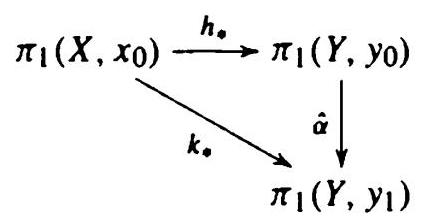
\includegraphics[width=0.3\textwidth]{images/58.25.jpg}
\end{center}
\hspace*{3em} 

\begin{proof}
	Let \(f : I \rightarrow  X\) be a loop in \(X\) based at \({x}_{0}\) . We must show that
\[
{k}_{ * }( [  f]  )  = \widehat{\alpha }( {h}_{ * }( [  f]  ) )
\]

This equation states that \([  {k \circ  f}]   = [  \bar{\alpha }]   * [  {h \circ  f}]   * [  \alpha ]\) , or equivalently, that

\[
[  \alpha ]   * [  {k \circ  f}]   = [  {h \circ  f}]   * [  \alpha ]  .
\]

This is the equation we shall verify.

To begin, consider the loops \({f}_{0}\) and \({f}_{1}\) in the space \(X \times  I\) given by the equations

\[
{f}_{0}( s)  = ( {f( s) ,0}) \;\text{ and }\;{f}_{1}( s)  = ( {f( s) ,1}) .
\]

Consider also the path \(c\) in \(X \times  I\) given by the equation

\[
c( t)  = ( {{x}_{0},t}) \text{ . }
\]

\begin{center}
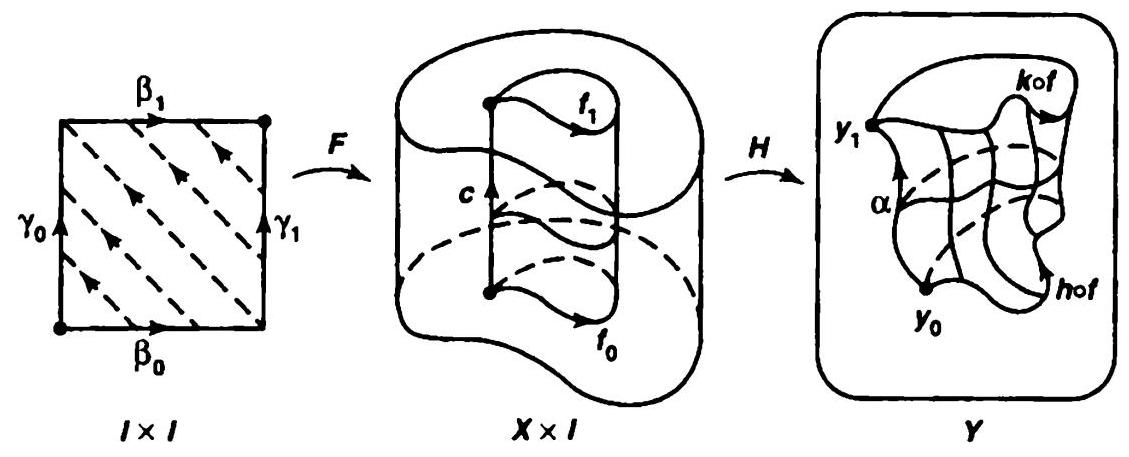
\includegraphics[width=1.0\textwidth]{images/58.3.jpg}
\end{center}
\hspace*{3em} 

Figure 58.3

Then \(H \circ  {f}_{0} = h \circ  f\) and \(H \circ  {f}_{1} = k \circ  f\) , while \(H \circ  c\) equals the path \(\alpha\) . See Figure 58.3.

Let \(F : I \times  I \rightarrow  X \times  I\) be the map \(F( {s,t})  = ( {f( s) ,t})\) . Consider the following paths in \(I \times  I\) , which run along the four edges of \(I \times  I\) :

\[
{\beta }_{0}( s)  = ( {s,0}) \;\text{ and }\;{\beta }_{1}( s)  = ( {s,1}) ,
\]

\[
{\gamma }_{0}( t)  = ( {0,t}) \;\text{ and }\;{\gamma }_{1}( t)  = ( {1,t}) .
\]

Then \(F \circ  {\beta }_{0} = {f}_{0}\) and \(F \circ  {\beta }_{1} = {f}_{1}\) , while \(F \circ  {\gamma }_{0} = F \circ  {\gamma }_{1} = c\) .

The broken-line paths \({\beta }_{0} * {\gamma }_{1}\) and \({\gamma }_{0} * {\beta }_{1}\) are paths in \(I \times  I\) from(0,0)to(1,1); since \(I \times  I\) is convex, there is a path homotopy \(G\) between them. Then \(F \circ  G\) is a path homotopy in \(X \times  I\) between \({f}_{0} * c\) and \(c * {f}_{1}\) . And \(H \circ  ( {F \circ  G})\) is a path homotopy in \(Y\) between

\[
( {H \circ  {f}_{0}})  * ( {H \circ  c})  = ( {h \circ  f})  * \alpha \;\text{ and }
\]

\[
( {H \circ  c})  * ( {H \circ  {f}_{1}})  = \alpha  * ( {k \circ  f}) ,
\]

as desired.
\end{proof}
\begin{corollary}
	Let \(h,k : X \rightarrow  Y\) be homotopic continuous maps; let \(h( {x}_{0})  = {y}_{0}\) and \(k( {x}_{0})  = {y}_{1}\) . If \({h}_{ * }\) is injective, or surjective, or trivial, so is \({k}_{ * }\) .
\end{corollary}

\begin{corollary}
	Let \(h : X \rightarrow  Y\) . If \(h\) is nulhomotopic, then \({h}_{ * }\) is the trivial homomorphism.
\end{corollary}

\begin{proof}
	The constant map induces the trivial homomorphism.
\end{proof}
\begin{theorem}
	Let \(f : X \rightarrow  Y\) be continuous; let \(f( {x}_{0})  = {y}_{0}\) . If \(f\) is a \index{homotopy equivalence@Homotopy equivalence}homotopy equivalence, then

\[
{f}_{ * } : {\pi }_{1}( {X,{x}_{0}})  \rightarrow  {\pi }_{1}( {Y,{y}_{0}})
\]

is an isomorphism.
\end{theorem}

\begin{proof}
	Let \(g : Y \rightarrow  X\) be a homotopy inverse for \(f\) . Consider the maps
\[
( {X,{x}_{0}}) \overset{f}{ \rightarrow  }( {Y,{y}_{0}}) \overset{g}{ \rightarrow  }( {X,{x}_{1}}) \overset{f}{ \rightarrow  }( {Y,{y}_{1}}) ,
\]

where \({x}_{1} = g( {y}_{0})\) and \({y}_{1} = f( {x}_{1})\) . We have the corresponding induced homomorphisms:

\begin{center}
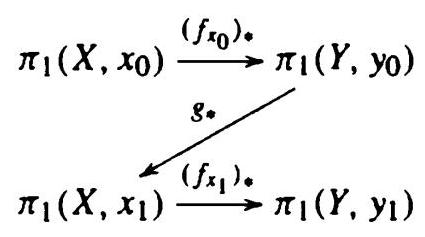
\includegraphics[width=0.3\textwidth]{images/58.35.jpg}
\end{center}
\hspace*{3em} 

[Here we have to distinguish between the homomorphisms induced by \(f\) relative to two different base points.] Now

\[
g \circ  f : ( {X,{x}_{0}})  \rightarrow  ( {X,{x}_{1}})
\]

is by hypothesis homotopic to the identity map, so there is a path \(\alpha\) in \(X\) such that

\[
{( g \circ  f) }_{ * } = \widehat{\alpha } \circ  {( i\chi ) }_{ * } = \widehat{\alpha }.
\]

It follows that \({( g \circ  f) }_{ * } = {g}_{ * } \circ  {( {f}_{{x}_{0}}) }_{ * }\) is an isomorphism.

Similarly, because \(f \circ  g\) is homotopic to the identity map \({iy}\) , the homomorphism \({( f \circ  g) }_{ * } = {( {f}_{{x}_{1}}) }_{ * } \circ  {g}_{ * }\) is an isomorphism.

The first fact implies that \({g}_{ * }\) is surjective, and the second implies that \({g}_{ * }\) is injective. Therefore, \({g}_{ * }\) is an isomorphism. Applying the first equation once again, we conclude that

\[
{( {f}_{{x}_{0}}) }_{ * } = {( {g}_{ * }) }^{-1} \circ  \widehat{\alpha },
\]

so that \({( {f}_{{x}_{0}}) }_{ * }\) is also an isomorphism.

Note that although \(g\) is a \index{homotopy inverse@Homotopy inverse}homotopy inverse for \(f\) , the homomorphism \({g}_{ * }\) is not an inverse for the homomorphism \({( {f}_{{x}_{0}}) }_{ * }\) .

The relation of homotopy equivalence is clearly more general than the notion \index{Fundamental group!of deformation retract}of deformation retraction. The theta space and the figure eight are both deformation retracts of the \index{doubly punctured plane@Doubly punctured plane}doubly punctured plane. Therefore, they are homotopy equivalent to the doubly punctured plane, and hence to each other. But neither is homeomorphic to a deformation retract of the other; in fact, neither of them can even be imbedded in the other.

It is a striking fact that the situation that occurs for these two spaces is the standard situation regarding homotopy equivalences. Martin Fuchs has proved a theorem to the effect that two spaces \(X\) and \(Y\) have the same \index{Contractible space!homotopy type}homotopy type if and only if they are homeomorphic to deformation retracts of a single space \(Z\) . The proof, although it uses only elementary tools, is difficult 		\cite{Fuchs1971}.
\end{proof}
\section*{Exercises}
\begin{enumerate}[itemsep=0.4em, parsep=0pt, topsep=0pt, partopsep=0pt, leftmargin=*, label=\arabic*., ref=\arabic*]
\item Show that if \(A\) is a deformation retract of \(X\) , and \(B\) is a deformation retract of \(A\) , then \(B\) is a deformation retract of \(X\) .
\item For each of the following spaces, the fundamental group is either trivial, infinite cyclic, or isomorphic to the fundamental group of the figure eight. Determine for each space which of the three alternatives holds.
  \begin{enumerate}[itemsep=0.2em, parsep=0pt, topsep=0pt, partopsep=0pt, leftmargin=*, label=(\alph*), align=left]
  \item The ``solid torus,'' \({B}^{2} \times  {S}^{1}\) .
  \item The torus \(T\) with a point removed.
  \item The cylinder \({S}^{1} \times  I\) .
  \item The infinite cylinder \({S}^{1} \times  \mathbb{R}\) .
  \item \({\mathbb{R}}^{3}\) with the nonnegative \(x,y\) , and \(z\) axes deleted. The following subsets of \({\mathbb{R}}^{2}\) :
  \item \(\{ x \mid  \parallel x\parallel  > 1\}\)
  \item \(\{ x \mid  \parallel x\parallel  \geq  1\}\)
  \item \(\{ x \mid  \parallel x\parallel  < 1\}\)
  \item \({S}^{1} \cup  ( {{\mathbb{R}}_{ + } \times  0})\)
  \item \({S}^{1} \cup  ( {{\mathbb{R}}_{ + } \times  \mathbb{R}})\)
  \item \({S}^{1} \cup  ( {\mathbb{R} \times  0})\)
  \item \({\mathbb{R}}^{2} - ( {{\mathbb{R}}_{ + } \times  0})\)
  \end{enumerate}
\item Show that given a collection \(\mathcal{C}\) of spaces, the relation of homotopy equivalence is an equivalence relation on \(\mathcal{C}\) .
\item Let \(X\) be the figure eight and let \(Y\) be the theta space. Describe maps \(f : X \rightarrow  Y\) and \(g : Y \rightarrow  X\) that are homotopy inverse to each other.
\item Recall that a space \(X\) is said to be contractible if the identity map of \(X\) to itself is nulhomotopic. Show that \(X\) is contractible if and only if \(X\) has the homotopy type of a one-point space.
\item Show that a retract of a contractible space is contractible.
\item Let \(A\) be a subspace of \(X\) ; let \(j : A \rightarrow  X\) be the inclusion map, and let \(f : X \rightarrow\)  \(A\) be a continuous map. Suppose there is a homotopy \(H : X \times  I \rightarrow  X\) between the map \(j \circ  f\) and the identity map of \(X\) .
  \begin{enumerate}[itemsep=0.2em, parsep=0pt, topsep=0pt, partopsep=0pt, leftmargin=*, label=(\alph*), align=left]
  \item Show that if \(f\) is a retraction, then \({j}_{ * }\) is an isomorphism.
  \item Show that if \(H\) maps \(A \times  I\) into \(A\) , then \({j}_{ * }\) is an isomorphism.
  \item Give an example in which \({j}_{ * }\) is not an isomorphism. *8. Find a space \(X\) and a point \({x}_{0}\) of \(X\) such that inclusion \(\{  {x}_{0}\}   \rightarrow  X\) is a homotopy equivalence, but \(\{  {x}_{0}\}\) is not a deformation retract of \(X\) . [Hint: Let \(X\) be the subspace of \({\mathbb{R}}^{2}\) that is the union of the line segments \(( {1/n})  \times  I\) , for \(n \in  {\mathbb{Z}}_{ + }\) , the line segment \(0 \times  I\) , and the line segment \(I \times  0\) ; let \({x}_{0}\) be the point(0,1). If \(\{  {x}_{0}\}\) is a deformation retract of \(X\) , show that for any neighborhood \(U\) of \({x}_{0}\) , the path component of \(U\) containing \({x}_{0}\) contains a neighborhood of \({x}_{0}\) .]
  \end{enumerate}
\item We define the degree of a continuous map \(h : {S}^{1} \rightarrow  {S}^{1}\) as follows: Let \({b}_{0}\) be the point(1,0)of \({S}^{1}\) ; choose a generator \(\gamma\) for the infinite cyclic group \({\pi }_{1}( {{S}^{1},{b}_{0}})\) . If \({x}_{0}\) is any point of \({S}^{1}\) , choose a path \(\alpha\) in \({S}^{1}\) from \({b}_{0}\) to \({x}_{0}\) , and define \(\gamma ( {x}_{0})  = \widehat{\alpha }( \gamma )\) . Then \(\gamma ( {x}_{0})\) generates \({\pi }_{1}( {{S}^{1},{x}_{0}})\) . The element \(\gamma ( {x}_{0})\) is independent of the choice of the path \(\alpha\) , since the fundamental group of \({S}^{1}\) is abelian. Now given \(h : {S}^{1} \rightarrow  {S}^{1}\) , choose \({x}_{0} \in  {S}^{1}\) and let \(h( {x}_{0})  = {x}_{1}\) . Consider the homomorphism \[ {h}_{ * } : {\pi }_{1}( {{S}^{1},{x}_{0}})  \rightarrow  {\pi }_{1}( {{S}^{1},{x}_{1}}) . \] Since both groups are infinite cyclic, we have (*) \[ {h}_{ * }( {\gamma ( {x}_{0}) })  = d \cdot  \gamma ( {x}_{1}) \] for some integer \(d\) , if the group is written additively. The integer \(d\) is called the degree of \(h\) and is denoted by \(\deg h\) . The degree of \(h\) is independent of the choice of the generator \(\gamma\) ; choosing the other generator would merely change the sign of both sides of \(( *)\) .
  \begin{enumerate}[itemsep=0.2em, parsep=0pt, topsep=0pt, partopsep=0pt, leftmargin=*, label=(\alph*), align=left]
  \item Show that \(d\) is independent of the choice of \({x}_{0}\) .
  \item Show that if \(h,k : {S}^{1} \rightarrow  {S}^{1}\) are homotopic, they have the same degree.
  \item Show that \(\deg ( {h \circ  k})  = ( {\deg h})  \cdot  ( {\deg k})\) .
  \item Compute the degrees of the constant map, the identity map, the reflection map \(\rho ( {{x}_{1},{x}_{2}})  = ( {{x}_{1}, - {x}_{2}})\) , and the map \(h( z)  = {z}^{n}\) , where \(z\) is a complex number. *(e) Show that if \(h,k : {S}^{1} \rightarrow  {S}^{1}\) have the same degree, they are homotopic.
  \end{enumerate}
\item Suppose that to every map \(h : {S}^{n} \rightarrow  {S}^{n}\) we have assigned an integer, denoted by deg \(h\) and called the degree of \(h\) , such that:
  \begin{enumerate}[itemsep=0.2em, parsep=0pt, topsep=0pt, partopsep=0pt, leftmargin=*, label=(\alph*), align=left]
  \item \index{homotopic maps@Homotopic maps} have the same degree. (ii) \(\deg ( {h \circ  k})  = ( {\deg h})  \cdot  ( {\deg k})\) . (iii) The identity map has degree 1, any constant map has degree 0, and the reflection map \(\rho ( {{x}_{1},\ldots ,{x}_{n + 1}})  = ( {{x}_{1},\ldots ,{x}_{n}, - {x}_{n + 1}})\) has degree-1. [One can construct such a function, using the tools of algebraic topology. Intuitively, \(\deg h\) measures how many times \(h\) wraps \({S}^{n}\) about itself; the sign tells you whether \(h\) preserves orientation or not.] Prove the following:
  \item There is no retraction \(r : {B}^{n + 1} \rightarrow  {S}^{n}\) .
  \item If \(h : {S}^{n} \rightarrow  {S}^{n}\) has degree different from \({( -1) }^{n + 1}\) , then \(h\) has a fixed point. [Hint: Show that if \(h\) has no fixed point, then \(h\) is homotopic to the \index{Antipodal map} \(a( x)  =  - x\) .]
  \item If \(h : {S}^{n} \rightarrow  {S}^{n}\) has degree different from 1, then \(h\) maps some point \(x\) to its antipode \(- x\) .
  \item If \({S}^{n}\) has a nonvanishing tangent vector field \(v\) , then \(n\) is odd. [Hint: If \(v\) exists, show the identity map is homotopic to the \index{antipodal map@Antipodal map}antipodal map.]
  \end{enumerate}
\end{enumerate}
\section*{§ 59 The Fundamental Group of \({S}^{n}\)}

Now we turn to a problem mentioned at the beginning of the chapter, the problem of showing that the sphere, torus, and double torus are surfaces that are topologically distinct. We begin with the sphere; we show that \({S}^{n}\) is simply connected for \(n \geq  2\) . The crucial result we need is stated in the following theorem.

\begin{theorem}
	Suppose \(X = U \cup  V\) , where \(U\) and \(V\) are open sets of \(X\) . Suppose that \(U \cap  V\) is path connected, and that \({x}_{0} \in  U \cap  V\) . Let \(i\) and \(j\) be the inclusion mappings of \(U\) and \(V\) , respectively, into \(X\) . Then the images of the induced homomorphisms

\[
{i}_{ * } : {\pi }_{1}( {U,{x}_{0}})  \rightarrow  {\pi }_{1}( {X,{x}_{0}}) \;\text{ and }\;{j}_{ * } : {\pi }_{1}( {V,{x}_{0}})  \rightarrow  {\pi }_{1}( {X,{x}_{0}})
\]

generate \({\pi }_{1}( {X,{x}_{0}})\) .
\end{theorem}

\begin{proof}
	This theorem states that, given any loop \(f\) in \(X\) based at \({x}_{0}\) , it is path homotopic to a product of the form \(( {{g}_{1} * ( {{g}_{2} * ( {\cdots  * {g}_{n}}) }) })\) , where each \({g}_{i}\) is a loop in \(X\) based at \({x}_{0}\) that lies either in \(U\) or in \(V\) .
Step 1. We show there is a subdivision \({a}_{0} < {a}_{1} < \cdots  < {a}_{n}\) of the unit interval such that \(f( {a}_{i})  \in  U \cap  V\) and \(f( [  {{a}_{i - 1},{a}_{i}}]  )\) is contained either in \(U\) or in \(V\) , for each \(i\) .

To begin, choose a subdivision \({b}_{0},\ldots ,{b}_{m}\) of \([  {0,1}]\) such that for each \(i\) , the set \(f( [  {{b}_{i - 1},{b}_{i}}]  )\) is contained in either \(U\) or \(V\) . (Use the Lebesgue number lemma.) If \(f( {b}_{i})\) belongs to \(U \cap  V\) for each \(i\) , we are finished. If not, let \(i\) be an index such that \(f( {b}_{i})  \notin  U \cap  V\) . Each of the sets \(f( [  {{b}_{i - 1},{b}_{i}}]  )\) and \(f( [  {{b}_{i},{b}_{i + 1}}]  )\) lies either in \(U\) or in \(V\) . If \(f( {b}_{i})  \in  U\) , then both of these sets must lie in \(U\) ; and if \(f( {b}_{i})  \in  V\) , both of them must lie in \(V\) . In either case, we may delete \({b}_{i}\) , obtaining a new subdivision \({\mathrm{c}}_{0}\) , \(\ldots ,{c}_{m - 1}\) that still satisfies the condition that \(f( [  {{c}_{i - 1},{c}_{i}}]  )\) is contained either in \(U\) or in \(V\) , for each \(i\) .

A finite number of repetitions of this process leads to the desired subdivision.

Step 2. We prove the theorem. Given \(f\) , let \({a}_{0},\ldots ,{a}_{n}\) be the subdivision constructed in Step 1. Define \({f}_{i}\) to be the path in \(X\) that equals the positive linear map of \([  {0,1}]\) onto \([  {{a}_{i - 1},{a}_{i}}]\) followed by \(f\) . Then \({f}_{i}\) is a path that lies either in \(U\) or in \(V\) , and by Theorem 51.3,

\[
[  f]   = [  {f}_{1}]   * [  {f}_{2}]   * \cdots  * [  {f}_{n}]  .
\]

For each \(i\) , choose a path \({\alpha }_{i}\) in \(U \cap  V\) from \({x}_{0}\) to \(f( {a}_{i})\) . (Here we use the fact that \(U \cap  V\) is path connected.) Since \(f( {a}_{0})  = f( {a}_{n})  = {x}_{0}\) , we can choose \({\alpha }_{0}\) and \({\alpha }_{n}\) to be the constant path at \({x}_{0}\) . See Figure 59.1.

Now we set

\[
{g}_{i} = ( {{\alpha }_{i - 1} * {f}_{i}})  * \overline{{\alpha }_{i}}
\]

for each \(i\) . Then \({g}_{i}\) is a loop in \(X\) based at \({x}_{0}\) whose image lies either in \(U\) or in \(V\) Direct computation shows that

\[
[  {g}_{1}]   * [  {g}_{2}]   * \cdots  * [  {g}_{n}]   = [  {f}_{1}]   * [  {f}_{2}]   * \cdots  * [  {f}_{n}]  .
\]

\begin{center}
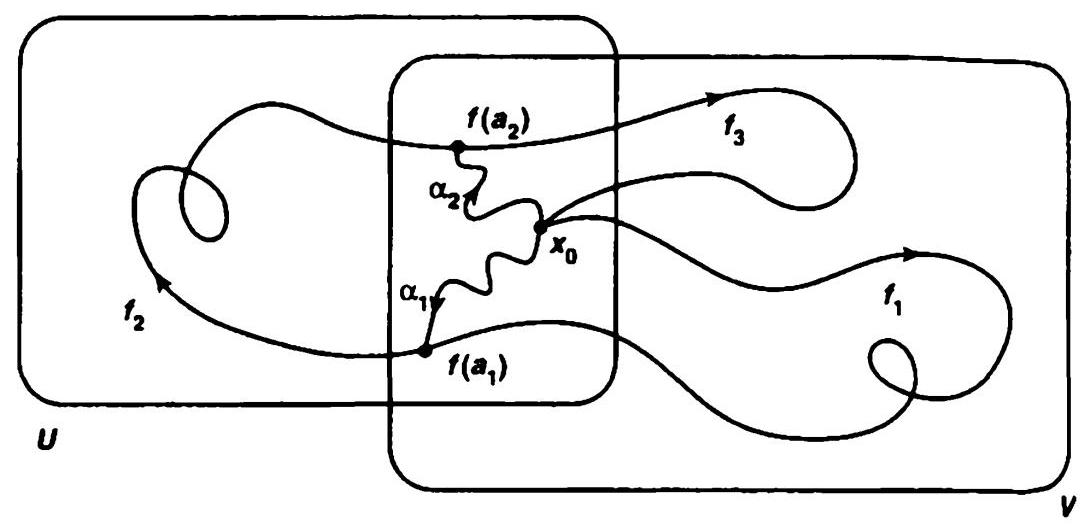
\includegraphics[width=1.0\textwidth]{images/59.1.jpg}
\end{center}
\hspace*{3em} 

Figure 59.1

The preceding theorem is a special case of a famous theorem of topology called the Seifert-van Kampen theorem, which expresses the fundamental group of the space \(X = U \cup  V\) quite generally, when \(U \cap  V\) is path connected, in terms of the fundamental groups of \(U\) and \(V\) . We shall study this theorem in \(C\) hapter 11 .
\end{proof}
\begin{corollary}
	Suppose \(X = U \cup  V\) , where \(U\) and \(V\) are open sets of \(X\) ; suppose \(U \cap  V\) is nonempty and path connected. If \(U\) and \(V\) are simply connected, then \(X\) is simply connected.
\end{corollary}

\begin{theorem}
	If \(n \geq  2\) , the \(n\) -sphere \({S}^{n}\) is \index{Simply connected!of \({S}^{n}\)}simply connected.
\end{theorem}

\begin{proof}
	Let \(p = ( {0,\ldots ,0,1})  \in  {\mathbb{R}}^{n + 1}\) and \(q = ( {0,\ldots ,0, - 1})\) be the ``north pole'' and the ``south pole'' of \({S}^{n}\) , respectively.
Step 1. We show that if \(n \geq  1\) , the punctured sphere \({S}^{n} - p\) is homeomorphic to \({\mathbb{R}}^{n}\) .

Define \(f : ( {{S}^{n} - p})  \rightarrow  {\mathbb{R}}^{n}\) by the equation

\[
f( x)  = f( {{x}_{1},\ldots ,{x}_{n + 1}})  = \frac{1}{1 - {x}_{n + 1}}( {{x}_{1},\ldots ,{x}_{n}}) .
\]

The map \(f\) is called \index{Stereographic projection}. (If one takes the straight line in \({\mathbb{R}}^{n + 1}\) passing through the north pole \(p\) and the point \(x\) of \({S}^{n} - p\) , then this line intersects the \(n\) -plane \({\mathbb{R}}^{n} \times  0 \subset  {\mathbb{R}}^{n + 1}\) in the point \(f( x)  \times  0\) .) One checks that \(f\) is a homeomorphism by showing that the map \(g : {\mathbb{R}}^{n} \rightarrow  ( {{S}^{n} - p})\) given by

\[
g( y)  = g( {{y}_{1},\ldots ,{y}_{n}})  = ( {t( y)  \cdot  {y}_{1},\ldots ,t( y)  \cdot  {y}_{n},1 - t( y) }) ,
\]

where \(t( y)  = 2/( {1 + \parallel y{\parallel }^{2}})\) , is a right and left inverse for \(f\) .

Note that the reflection map \(( {{x}_{1},\ldots ,{x}_{n + 1}})  \rightarrow  ( {{x}_{1},\ldots ,{x}_{n}, - {x}_{n + 1}})\) defines a homeomorphism of \({S}^{n} - p\) with \({S}^{n} - q\) , so the latter is also homeomorphic to \({\mathbb{R}}^{n}\) .

Step 2. We prove the theorem. Let \(U\) and \(V\) be the open sets \(U = {S}^{n} - p\) and \(V = {S}^{n} - q\) of \({S}^{n}.\)

Note first that for \(n \geq  1\) , the sphere \({S}^{n}\) is \index{Path connectedness!of \({S}^{n}\)}path connected. This follows from the fact that \(U\) and \(V\) are path connected (being homeomorphic to \({\mathbb{R}}^{n}\) ) and have the point \(( {1,0,\ldots ,0})\) of \({S}^{n}\) in common.

Now we show that for \(n \geq  2\) , the sphere \({S}^{n}\) is simply connected. The spaces \(U\) and \(V\) are simply connected, being homeomorphic to \({\mathbb{R}}^{n}\) . Their intersection equals \({S}^{n} - p - q\) , which is homeomorphic under \index{stereographic projection@Stereographic projection}stereographic projection to \({\mathbb{R}}^{n} - \mathbf{0}\) . The latter space is path connected, for every point of \({\mathbb{R}}^{n} - 0\) can be joined to a point of \({S}^{n - 1}\) by a straight-line path, and \({S}^{n - 1}\) is path connected if \(n \geq  2\) . Then the preceding corollary applies.
\end{proof}
\section*{Exercises}
\begin{enumerate}[itemsep=0.4em, parsep=0pt, topsep=0pt, partopsep=0pt, leftmargin=*, label=\arabic*., ref=\arabic*]
\item Let \(X\) be the union of two copies of \({S}^{2}\) having a single point in common. What is the fundamental group of \(X\) ? Prove that your answer is correct. [Be careful! The union of two simply connected spaces having a point in common is not necessarily simply connected. See 		\cite{Spanier1966}, p. 59.]
\item Criticize the following ``proof'' that \({S}^{2}\) is simply connected: Let \(f\) be a loop in \({S}^{2}\) based at \({x}_{0}\) . Choose a point \(p\) of \({S}^{2}\) not lying in the image of \(f\) . Since \({S}^{2} - p\) is homeomorphic with \({\mathbb{R}}^{2}\) , and \({\mathbb{R}}^{2}\) is simply connected, the loop \(f\) is path homotopic to the constant loop.
\item
  \begin{enumerate}[itemsep=0.2em, parsep=0pt, topsep=0pt, partopsep=0pt, leftmargin=*, label=(\alph*), align=left]
  \item Show that \({\mathbb{R}}^{1}\) and \({\mathbb{R}}^{n}\) are not homeomorphic if \(n > 1\) .

  \item Show that \({\mathbb{R}}^{2}\) and \({\mathbb{R}}^{n}\) are not homeomorphic if \(n > 2\) . It is, in fact, true that \({\mathbb{R}}^{m}\) and \({\mathbb{R}}^{n}\) are not homeomorphic if \(n \neq  m\) , but the proof requires more advanced tools of algebraic topology.
  \end{enumerate}
\item Assume the hypotheses of Theorem 59.1.
  \begin{enumerate}[itemsep=0.2em, parsep=0pt, topsep=0pt, partopsep=0pt, leftmargin=*, label=(\alph*), align=left]
  \item What can you say about the fundamental group of \(X\) if \({j}_{ * }\) is the trivial homomorphism? If both \({i}_{ * }\) and \({j}_{ * }\) are trivial?
  \item Give an example where \({i}_{ * }\) and \({j}_{ * }\) are trivial but neither \(U\) nor \(V\) have trivial fundamental groups
  \end{enumerate}
\end{enumerate}
\section*{§ 60 Fundamental Groups of Some Surfaces}

Recall that a surface is a Hausdorff space with a countable basis, each point of which has a neighborhood that is homeomorphic with an open subset of \({\mathbb{R}}^{2}\) . Surfaces are of interest in various parts of mathematics, including geometry, topology, and complex analysis. We consider here several surfaces, including the torus and double torus, and show by comparing their fundamental groups that they are not homeomorphic. In a later chapter, we shall classify up to homeomorphism all compact surfaces.

First, we consider the torus. In an earlier exercise, we asked you to compute its fundamental group using the theory of covering spaces. Here, we compute its fundamental group by using a theorem about the fundamental group \index{Fundamental group!of a product}of a product space.

Recall that if \(A\) and \(B\) are groups with operation \(\cdot\) , then the cartesian product \(A \times  B\) is given a group structure by using the operation

\[
( {a \times  b})  \cdot  ( {{a}^{\prime } \times  {b}^{\prime }})  = ( {a \cdot  {a}^{\prime }})  \times  ( {b \cdot  {b}^{\prime }}) .
\]

Recall also that if \(h : C \rightarrow  A\) and \(k : C \rightarrow  B\) are group homomorphisms, then the map \(\Phi  : C \rightarrow  A \times  B\) defined by \(\Phi ( c)  = h( c)  \times  k( c)\) is a group homomorphism.

\begin{theorem}
	\({\pi }_{1}( {X \times  Y,{x}_{0} \times  {y}_{0}})\) is isomorphic with \({\pi }_{1}( {X,{x}_{0}})  \times  {\pi }_{1}( {Y,{y}_{0}})\) .
\end{theorem}

\begin{proof}
	Let \(p : X \times  Y \rightarrow  X\) and \(q : X \times  Y \rightarrow  Y\) be the projection mappings. If we use the base points indicated in the statement of the theorem, we have induced homomorphisms
\[
{p}_{ * } : {\pi }_{1}( {X \times  Y,{x}_{0} \times  {y}_{0}})  \rightarrow  {\pi }_{1}( {X,{x}_{0}}) ,
\]

\[
{q}_{ * } : {\pi }_{1}( {X \times  Y,{x}_{0} \times  {y}_{0}})  \rightarrow  {\pi }_{1}( {Y,{y}_{0}}) .
\]

We define a homomorphism

\[
\Phi  : {\pi }_{1}( {X \times  Y,{x}_{0} \times  {y}_{0}})  \rightarrow  {\pi }_{1}( {X,{x}_{0}})  \times  {\pi }_{1}( {Y,{y}_{0}})
\]

by the equation

\[
\Phi ( [  f]  )  = {p}_{ * }( [  f]  )  \times  {q}_{ * }( [  f]  )  = [  {p \circ  f}]   \times  [  {q \circ  f}]  .
\]

We shall show that \(\Phi\) is an isomorphism.

The map \(\Phi\) is surjective. Let \(g : I \rightarrow  X\) be a loop based at \({x}_{0}\) ; let \(h : I \rightarrow  Y\) be a loop based at \({y}_{0}\) . We wish to show that the element \([  g]   \times  [  h]\) lies in the image of \(\Phi\) . Define \(f : I \rightarrow  X \times  Y\) by the equation

\[
f( s)  = g( s)  \times  h( s) .
\]

Then \(f\) is a loop in \(X \times  Y\) based at \({x}_{0} \times  {y}_{0}\) , and

\[
\Phi ( [  f]  )  = [  {p \circ  f}]   \times  [  {q \circ  f}]   = [  g]   \times  [  h]  ,
\]

as desired.

The kernel of \(\Phi\) vanishes. Suppose that \(f : I \rightarrow  X \times  Y\) is a loop in \(X \times  Y\) based at \({x}_{0} \times  {y}_{0}\) and \(\Phi ( [  f]  )  = [  {p \circ  f}]   \times  [  {q \circ  f}]\) is the identity element. This means that \(p \circ  f{ \simeq  }_{p}{e}_{{x}_{0}}\) and \(q \circ  f{ \simeq  }_{p}{e}_{{y}_{0}}\) ; let \(G\) and \(H\) be the respective path homotopies. Then the map \(F : I \times  I \rightarrow  X \times  Y\) defined by

\[
F( {s,t})  = G( {s,t})  \times  H( {s,t})
\]

is a path homotopy between \(f\) and the constant loop based at \({x}_{0} \times  {y}_{0}\) .
\end{proof}
\begin{corollary}
	The fundamental group of the torus \(T = {S}^{1} \times  {S}^{1}\) is isomorphic to the group \(\mathbb{Z} \times  \mathbb{Z}\) .
\end{corollary}

Now we define a surface called the \index{projective n-space@Projective n-space} projective plane and compute its fundamental group.

\begin{definition}
	The projective plane \(\index{P@\({P}^{2}\)} \index{P@${P}^{2}$}\index{P@${P}^{2}$}\index{P@${P}^{2}$}{P}^{2}\) is the quotient space obtained from \({S}^{2}\) by identifying each point \(x\) of \({S}^{2}\) with its antipodal point \(- x\) .
\end{definition}

The projective plane may not be a space that is familiar to you; it cannot be imbedded in \({\mathbb{R}}^{3}\) and is thus difficult to visualize. It is, however, the fundamental object \index{Covering space!of \({\mathbb{R}}^{2} - 0\)}of study in projective geometry, just as the euclidean plane \({\mathbb{R}}^{2}\) is in ordinary euclidean geometry. Topologists are primarily interested in it as an example \index{Covering space!of \({P}^{2}\)}of a surface.

\begin{theorem}
	The projective plane \({P}^{2}\) is a compact surface, and the quotient map \(p : {S}^{2} \rightarrow  {P}^{2}\) is a \index{covering map@Covering map}covering map.
\end{theorem}

\begin{proof}
	First we show that \(p\) is an open map. Let \(U\) be open in \({S}^{2}\) . Now the \index{antipodal map@Antipodal map}antipodal map \(a : {S}^{2} \rightarrow  {S}^{2}\) given by \(a( x)  =  - x\) is a homeomorphism of \({S}^{2}\) ; hence \(a( U)\) \index{Covering map!is open}is open in \({S}^{2}\) . Since
\[
{p}^{-1}( {p( U) })  = U \cup  a( U)
\]

this set also \index{Covering map!is open}is open in \({S}^{2}\) . Therefore, by definition, \(p( U)\) is open in \({P}^{2}\) . A similar proof shows that \(p\) is a closed map.

Now we show that \(p\) is a \index{covering map@Covering map}covering map. Given a point \(y\) of \({P}^{2}\) , choose \(x \in  {p}^{-1}( y)\) . Then choose an \(\epsilon\) -neighborhood \(U\) of \(x\) in \({S}^{2}\) for some \(\epsilon  < 1\) , using the euclidean metric \(d\) of \({\mathbb{R}}^{3}\) . Then \(U\) contains no pair \(\{ z,a( z) \}\) of antipodal points of \({S}^{2}\) , since \(d( {z,a( z) })  = 2\) . As a result, the map

\[
p : U \rightarrow  p( U)
\]

is bijective. Being continuous and open, it is a homeomorphism. Similarly,

\[
p : a( U)  \rightarrow  p( {a( U) })  = p( U)
\]

is a homeomorphism. The set \({p}^{-1}( {p( U) })\) is thus the union of the two disjoint open sets \(U\) and \(a( U)\) , each of which is mapped homeomorphically by \(p\) onto \(p( U)\) . Then \(p( U)\) is a neighborhood of \(p( x)  = y\) that is \index{evenly covered@Evenly covered}evenly covered by \(p\) .

Since \({S}^{2}\) has a countable basis \(\{  {U}_{n}\}\) , the space \({P}^{2}\) has a countable basis \(\{  {p( {U}_{n}) }\}\) .

The fact that \({P}^{2}\) is Hausdorff follows from the fact that \({S}^{2}\) is normal and \(p\) is a closed map. (See Exercise 6 of §31.) Alternatively, one can give a direct proof: Let \({y}_{1}\) and \({y}_{2}\) be two points of \({P}^{2}\) . The set \({p}^{-1}( {y}_{1})  \cup  {p}^{-1}( {y}_{2})\) consists of four points; let \({2\epsilon }\) be the minimum distance between them. Let \({U}_{1}\) be the \(\epsilon\) -neighborhood of one of the points of \({p}^{-1}( {y}_{1})\) , and let \({U}_{2}\) be the \(\epsilon\) -neighborhood of one of the points of \({p}^{-1}( {y}_{2})\) . Then

\[
{U}_{1} \cup  a( {U}_{1}) \;\text{ and }\;{U}_{2} \cup  a( {U}_{2})
\]

are disjoint. It follows that \(p( {U}_{1})\) and \(p( {U}_{2})\) are disjoint neighborhoods of \({y}_{1}\) and \({y}_{2}\) , respectively, in \({P}^{2}\) .

Since \({S}^{2}\) is a surface and every point of \({P}^{2}\) has a neighborhood homeomorphic with an open subset of \({S}^{2}\) , the space \({P}^{2}\) is also a surface.
\end{proof}
\begin{corollary}
	\({\pi }_{1}( {{P}^{2},y})\) is a group of order 2 .
\end{corollary}

\begin{proof}
	The projection \(p : {S}^{2} \rightarrow  {P}^{2}\) is a covering map. Since \({S}^{2}\) is simply connected, we can apply Theorem 54.4, which tells us there is a bijective correspondence between \({\pi }_{1}( {{P}^{2},y})\) and the set \({p}^{-1}( y)\) . Since this set is a two-element set, \({\pi }_{1}( {{P}^{2},y})\) is a group of \index{order of a group@Order of a group}order 2.
Any group of order 2 is isomorphic to \(\mathbb{Z}/2\) , the integers mod 2, of course.

One can proceed similarly to define \({P}^{n}\) , for any \(n \in  {\mathbb{Z}}_{ + }\) , as the space obtained from \({S}^{n}\) by identifying each point \(x\) with its \index{antipode@Antipode}antipode \(- x\) ; it is called projective \(n\) - space. The proof of Theorem 60.3 goes through without change to prove that the projection \(p : {S}^{n} \rightarrow  {P}^{n}\) is a covering map. Then because \({S}^{n}\) is simply connected for \(n \geq  2\) , it follows that \({\pi }_{1}( {{P}^{n},y})\) is a two-element group for \(n \geq  2\) . We leave it to you to figure out what happens when \(n = 1\) .

Now we study the double torus. We begin with a lemma about the figure eight.
\end{proof}
\section*{Lemma 60.5. The fundamental group of the figure eight is not abelian.}

\begin{proof}
	Let \(X\) be the union of two circles \(A\) and \(B\) in \({\mathbb{R}}^{2}\) whose intersection consists of the single point \({x}_{0}\) . We describe a certain \index{covering space@Covering space}covering space \(E\) of \(X\) .
The space \(E\) is the subspace of the plane consisting of the \(x\) -axis and the \(y\) -axis, along with tiny circles tangent to these axes, one circle tangent to the \(x\) -axis at each nonzero integer point and one circle tangent to the \(y\) -axis at each nonzero integer point.

The projection map \(p : E \rightarrow  X\) wraps the \(x\) -axis around the circle \(A\) and wraps the \(y\) -axis around the other curcle \(B\) ; in each case the integer points are mapped by \(p\) into the \index{base point@Base point}base point \({x}_{0}\) . Each circle tangent to an integer point on the \(x\) -axis is mapped homeomorphically by \(p\) onto \(B\) , while each circle tangent to an integer point on the \(y\) -axis is mapped homeomorphically onto \(A\) ; in each case the point of targency is mapped onto the point \({x}_{0}\) . We leave it to you to check mentally that the map \(p\) is indeed a covering map.

We could write this description down in equations if we wished, but the informal description seems to us easier to follow.

Now let \(\bar{f} : I \rightarrow  E\) be the path \(\widetilde{f}( s)  = s \times  0\) , going along the \(x\) -axis from the origin to the point \(1 \times  0\) . Let \(\widetilde{g} : I \rightarrow  E\) be the path \(\bar{g}( s)  = 0 \times  s\) , going along the \(y\) -axis from the origin to the point \(0 \times  1\) . Let \(f = p \circ  \widetilde{f}\) and \(g = p \circ  \widetilde{g}\) ; then \(f\) and \(g\) are \index{loop@Loop}loops in the figure eight based at \({x}_{0}\) , going around the circles \(A\) and \(B\) , respectively. See Figure 60.1.

We assert that \(f * g\) and \(g * f\) are not path homotopic, so that the fundamental group \index{Covering space!of figure eight}of the figure eight is not abelian.

\begin{center}
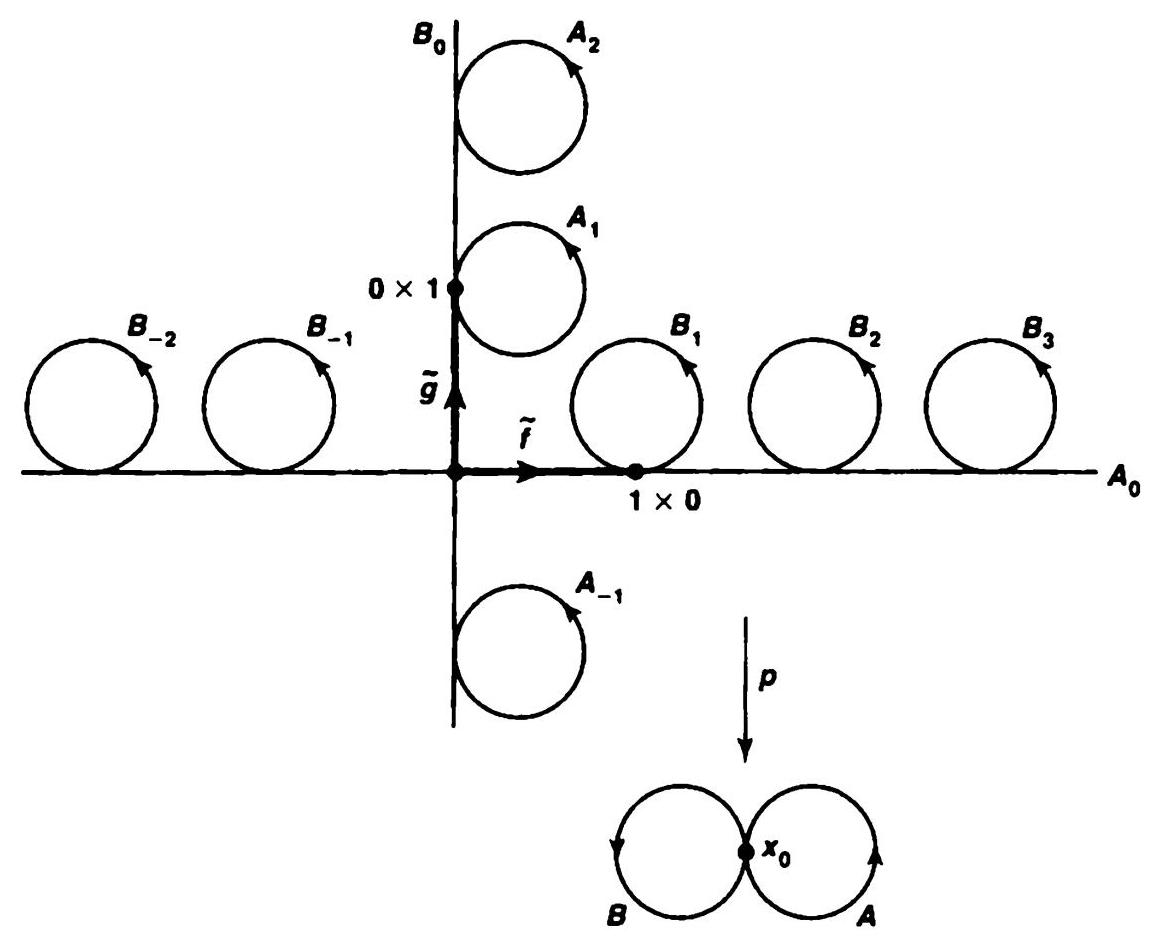
\includegraphics[width=1.0\textwidth]{images/60.1.jpg}
\end{center}
\hspace*{3em} 

Figure 60.1

To prove this assertion, let us lift each of these to a path in \(E\) beginning at the origin. The path \(f * g\) lifts to a path that goes along the \(x\) -axis from the origin to \(1 \times  0\) and then goes once around the circle tangent to the \(x\) -axis at \(1 \times  0\) . On the other hand, the path \(g * f\) lifts to a path in \(E\) that goes along the \(y\) -axis from the origin to \(0 \times  1\) , and then goes once around the circle tangent to the \(y\) -axis at \(0 \times  1\) . Since the lifted paths do not end at the same point, \(f * g\) and \(g * f\) cannot be path homotopic.

We shall prove later that the fundamental group of the figure eight is, in fact, the group that algebraists call the ``free group on two generators.''
\end{proof}
\section*{Theorem 60.6. The fundamental group of the double torus is not abelian.}

\begin{proof}
	The double torus \(T\# T\) is the surface obtained by taking two copies of the torus, deleting a small open disc from each of them, and pasting the remaining pieces together along their edges. We assert that the figure eight \(X\) is a retract of \(T\# T\) . This fact implies that inclusion \(j : X \rightarrow  T\# T\) induces a monomorphism \({j}_{ * }\) , so that \({\pi }_{1}( {T\# T,{x}_{0}})\) is not abelian.
One can write equations for the \index{retraction@Retraction}retraction \(r : T\# T \rightarrow  X\) , but it is simpler to indicate it in pictures, as we have done in Figure 60.2. Let \(Y\) be the union of two tori having a point in common. First one maps \(T\# T\) onto \(Y\) by a map that collapses the dotted curcle to a point but is otherwise one-to-one; it defines a homeomorphism \(h\) of the figure eight in \(T\# T\) with the figure eight in \(Y\) . Then one retracts \(Y\) onto its figure eight by mapping each cross-sectional circle to the point where it intersects the figure eight. Then one maps the figure eight in \(Y\) back onto the figure eight in \(T\# T\) by the map \({h}^{-1}\) .

\begin{center}
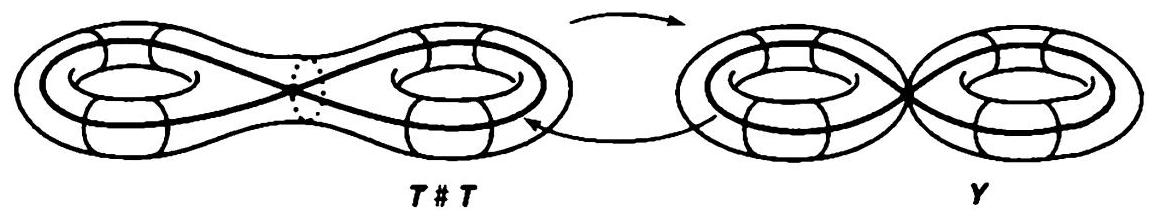
\includegraphics[width=1.0\textwidth]{images/60.2.jpg}
\end{center}
\hspace*{3em} 

Figure 60.2
\end{proof}
\begin{corollary}
	The 2-sphere, torus, projective plane, and double torus are topologically distinct.
\end{corollary}

\section*{Exercises}
\begin{enumerate}[itemsep=0.4em, parsep=0pt, topsep=0pt, partopsep=0pt, leftmargin=*, label=\arabic*., ref=\arabic*]
\item Compute the fundamental groups of the ``solid torus'' \({S}^{1} \times  {B}^{2}\) and the product space \({S}^{1} \times  {S}^{2}\) .
\item Let \(X\) be the quotient space obtained from \({B}^{2}\) by identifying each point \(x\) \index{Covering space!of \({S}^{1}\)}of \({S}^{1}\) with its \index{antipode@Antipode}antipode \(- x\) . Show that \(X\) is homeomorphic to the projective plane \({P}^{2}\) .
\item Let \(p : E \rightarrow  X\) be the map constructed in the proof of Lemma 60.5. Let \({E}^{\prime }\) be the subspace of \(E\) that is the union of the \(x\) -axis and the \(y\) -axis. Show that \(p \mid  {E}^{\prime }\) is not a covering map.
\item The space \({P}^{1}\) and the covering map \(p : {S}^{1} \rightarrow  {P}^{1}\) are familiar ones. What are they?
\item Consider the covering map indicated in Figure 60.3. Here, \(p\) wraps \({A}_{1}\) around \(A\) twice and wraps \({B}_{1}\) around \(B\) twice; \(p\) maps \({A}_{0}\) and \({B}_{0}\) homeomorphically onto \(A\) and \(B\) , respectively. Use this \index{Torus!covering space of}covering space to show that the fundamental group of the figure eight is not abelian. \begin{center} 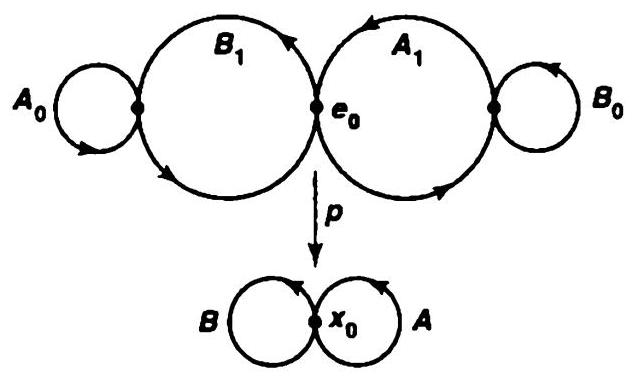
\includegraphics[width=0.5\textwidth]{images/60.3.jpg} \end{center} \hspace*{3em} Figure 60.3
\end{enumerate}
\chapter[Separation Theorems in the Plane]{Separation Theorems \\in the Plane}
\vspace{6.5cm}
\chaptermark{Separation Theorems in the Plane}


There are several difficult questions concerning the topology of the plane that arise quite naturally in the study of analysis. The answers to these questions seem geometrically quite obvious but turn out to be surprisingly hard to prove. They include the \index{jordan curve theorem@Jordan curve theorem}, the Brouwer theorem on \index{Invariance of domain}, and the classical theorem that the \index{Winding number} of a simple \index{closed topologist's sine curve@Closed topologist's sine curve} closed curve is zero or \(\pm  1\) . We prove them in this chapter as consequences \index{Fundamental group!of double torus}of our study of covering spaces and the \index{Double torus!fundamental group}fundamental group

\section*{§ 61 The Jordan Separation Theorem}

We consider first one of the classical theorems of mathematics, the \index{jordan curve theorem@Jordan curve theorem}Jordan curve theorem. It states a fact that is geometrically quite believable, the fact that a \index{Simple closed curve!separates \({S}^{2}\)}\index{simple closed curve@Simple closed curve}simple closed curve in the plane always \index{separates a space@Separates a space} separates the plane into two pieces, its ``inside'' and its ``outside.'' It was originally conjectured in 1892 by Camille Jordan, and several incorrect proofs were published, including one by Jordan himself. Eventually, a correct proof was provided by Oswald Veblen, in 1905. The early proofs were complicated, but over the years, simpler proofs have been found. If one uses the tools of modern algebraic topology, singular homology theory in particular, the proof is quite straightforward. The proof we give here is the simplest one we know that uses only results from the theory of covering spaces and the fundamental group.

Our proof of the Jordan curve theorem divides into three parts. The first, which we call the \index{jordan separation theorem@Jordan separation theorem}, states that a simple closed curve in the plane separates it into at least two components. The second says that an arc in the plane does not separate the plane. And the third, the Jordan curve theorem proper, says that a simple closed curve \(C\) in the plane separates it into precisely two components, of which \(C\) is the common boundary. The first of these theorems will be treated in this section.

In dealing with separation theorems, it will often be convenient to formulate them as separation theorems for subsets of \({S}^{2}\) rather than \({\mathbb{R}}^{2}\) . The separation theorems for \({\mathbb{R}}^{2}\) will follow. The connection between the two sets of theorems is provided by the following lemma.

Recall that if \(b\) is any point of \({S}^{2}\) , there is a homeomorphism \(h\) of \({S}^{2} - b\) with \({\mathbb{R}}^{2}\) ; one simply takes a rotation of \({S}^{2}\) that carries \(b\) to the north pole, and follows it by stereographic projection.

\begin{lemma}
	Let \(C\) be a compact subspace of \({S}^{2}\) ; let \(b\) be a point of \({S}^{2} - C\) ; and let \(h\) be a homeomorphism of \({S}^{2} - b\) with \({\mathbb{R}}^{2}\) . Suppose \(U\) is a component of \({S}^{2} - C\) . If \(U\) does not contain \(b\) , then \(h( U)\) is a bounded component of \({\mathbb{R}}^{2} - h( C)\) . If \(U\) contains \(b\) , then \(h( {U - b})\) is the unbounded component of \({\mathbb{R}}^{2} - h( C)\) .
\end{lemma}

In particular, if \({S}^{2} - C\) has \(n\) components, then \({\mathbb{R}}^{2} - h( C)\) has \(n\) components.

\begin{proof}
	We show first that if \(U\) is a component of \({S}^{2} - C\) , then \(U - b\) is connected. This result is trivial if \(b \notin  U\) , so suppose that \(b \in  U\) and suppose the sets \(A\) and \(B\) form a separation of \(U - b\) . Choose a neighborhood \(W\) of \(b\) disjoint from \(C\) such that \(W\) is homeomorphic to an open ball of \({\mathbb{R}}^{2}\) . Since \(W\) is connected, it is contained in \(U\) ; since \(W - b\) is connected, it is contained entirely in \(A\) or in \(B\) . Say \(W - b \subset  A\) . Then \(b\) is not a limit point of \(B\) , for \(W\) is a neighborhood of \(b\) disjoint from \(B\) . It follows that the sets \(A \cup  \{ b\}\) and \(B\) form a separation of \(U\) , contrary to hypothesis.
Let \(\{  {U}_{\alpha }\}\) be the set of components of \({S}^{2} - C\) ; let \({V}_{\alpha } = h( {{U}_{\alpha } - b})\) . Because \({S}^{2} - C\) is locally connected, the sets \({U}_{\alpha }\) are connected, disjoint, open subsets of \({S}^{2}\) . Therefore, the sets \({V}_{\alpha }\) are connected, disjoint, open subsets of \({\mathbb{R}}^{2} - h( C)\) , so the sets \({V}_{\alpha }\) are the components of \({\mathbb{R}}^{2} - h( C)\) .

Now the homeomorphism \(h\) of \({S}^{2} - b\) with \({\mathbb{R}}^{2}\) can be extended to a homeomorphism \(H\) of \({S}^{2}\) with the one-point compactification \({\mathbb{R}}^{2} \cup  \{ \infty \}\) of \({\mathbb{R}}^{2}\) , merely by setting \(H( b)  = \infty\) . If \({U}_{\beta }\) is the component of \({S}^{2} - C\) containing \(b\) , then \(H( {U}_{\beta })\) is a neighborhood of \(\infty\) in \({\mathbb{R}}^{2} \cup  \{ \infty \}\) . Therefore \({V}_{\beta }\) is unbounded; since its complement \({\mathbb{R}}^{2} - {V}_{\beta }\) is compact, all the other components of \({\mathbb{R}}^{2} - h( C)\) are bounded. See Figure 61.1.
\end{proof}
\begin{lemma}[Null \index{free homotopy of loops@Free homotopy of loops}homotopy lemma]
	Let \(a\) and \(b\) be points of \({S}^{2}\) . Let \(A\) be a compact space, and let

\[
f : A \rightarrow  {S}^{2} - a - b
\]

be a continuous map. If \(a\) and \(b\) lie in the same component of \({S}^{2} - f( A)\) , then \(f\) is nulhomotopic.

\begin{center}
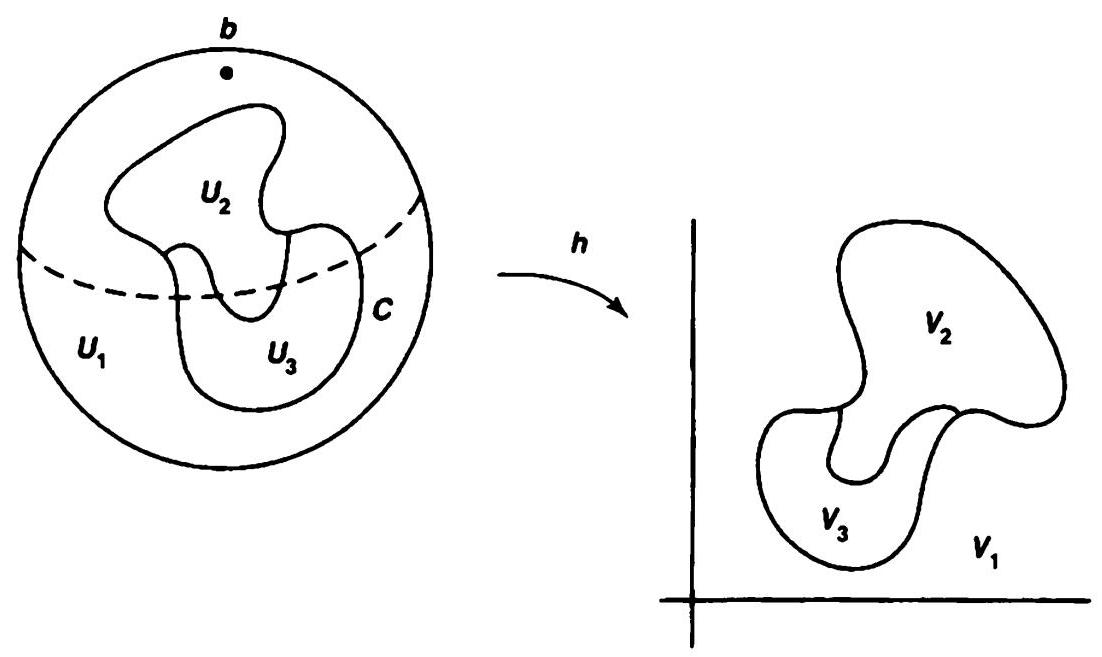
\includegraphics[width=1.0\textwidth]{images/61.1.jpg}
\end{center}
\hspace*{3em} 

Figure 61.1
\end{lemma}

\begin{proof}
	One can replace \({S}^{2}\) by the one-point compactification \({\mathbb{R}}^{2} \cup  \{ \infty \}\) of \({\mathbb{R}}^{2}\) , letting \(a\) and \(b\) correspond to the points0and \(\infty\) . Then our lemma reduces to the following: Let \(A\) be a compact space and let \(g : A \rightarrow  {\mathbb{R}}^{2} - 0\) be a continuous map. If0lies in the unbounded component of \({\mathbb{R}}^{2} - g( A)\) , then \(g\) is nulhomotopic.
This statement is easy to prove. Choose a ball \(B\) centered at the orgin, of sufficiently large radius that it contains the set \(g( A)\) . Choose a point \(p\) of \({\mathbb{R}}^{2}\) lying outside \(B\) . Then0and \(p\) both lie in the unbounded component of \({\mathbb{R}}^{2} - g( A)\) .

Because \({\mathbb{R}}^{2}\) is locally path connected, so is the open set \({\mathbb{R}}^{2} - g( A)\) . Therefore, the components and path components of \({\mathbb{R}}^{2} - g( A)\) are the same. Hence we can choose a path \(\alpha\) in \({\mathbb{R}}^{2} - g( A)\) from 0 to \(p\) . We define a homotopy \(G : A \times  I \rightarrow  {\mathbb{R}}^{2} -\) 0 by the equation

\[
G( {x,t})  = g( x)  - \alpha ( t) ;
\]

it is pictured in Figure 61.2. The homotopy \(G\) is a homotopy between the map \(g\) and the map \(k\) defined by \(k( x)  = g( x)  - p\) . Note that \(G( {x,t})  \neq  0\) because the path \(\alpha\) does not intersect the set \(g( A)\) .

Now we define a homotopy \(H : A \times  I \rightarrow  {\mathbb{R}}^{2} - 0\) by the equation

\[
H( {x,t})  = \operatorname{tg}( x)  - p.
\]

It is a homotopy between the map \(k\) and a constant map. Note that \(H( {x,t})  \neq  0\) because \({tg}( x)\) lies inside the ball \(B\) and \(p\) does not.

Thus we have proved that \(g\) is nulhomotopic.

Now we prove the \index{jordan separation theorem@Jordan separation theorem}Jordan separation theorem. In \index{Nonseparation theorem: arc in \({S}^{2}\)!general}general, if \(X\) is a connected space and \(A \subset  X\) , we say that \(A\) separates \(X\) if \(X - A\) is not connected; if \(X - A\) has \(n\) components, we say that \(A\) \index{separates a space@Separates a space}separates \(X\) \index{Separates a space!into \(n\) components}into n components.

\begin{center}
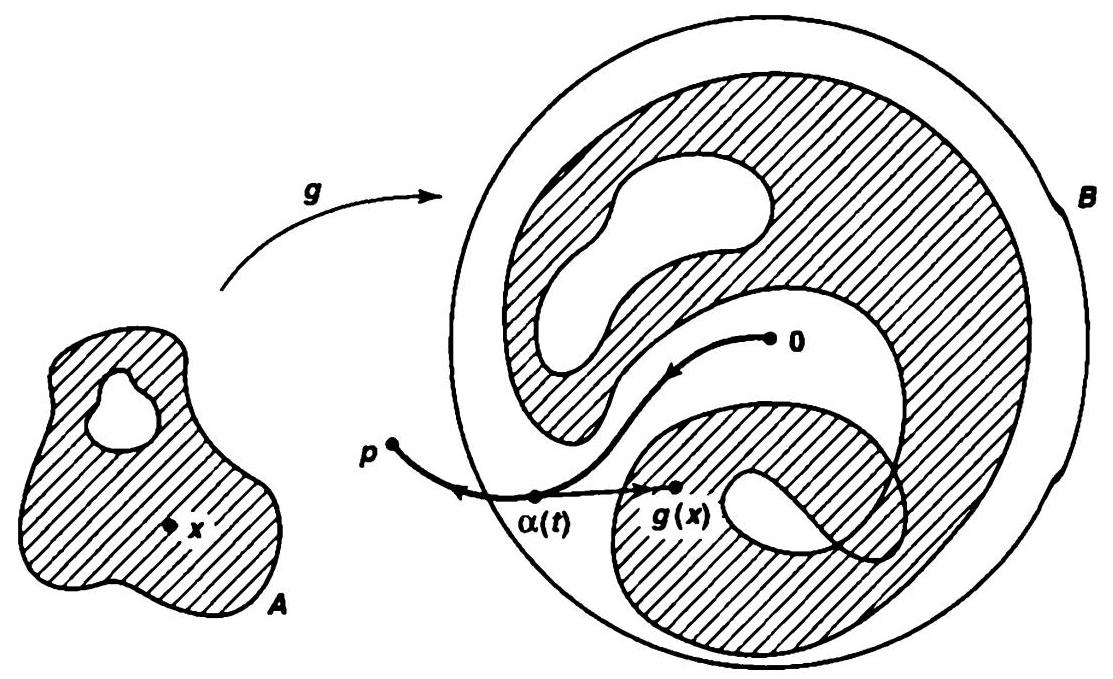
\includegraphics[width=1.0\textwidth]{images/61.2.jpg}
\end{center}
\hspace*{3em} 

Figure 61.2

An arc \(A\) is a space homeomorphic to the unit interval \([  {0,1}]\) . The end points of \(A\) are the two points \(p\) and \(q\) of \(A\) such that \(A - p\) and \(A - q\) are connected; the other points of \(A\) are called \index{interior point: of an arc@Interior point: of an arc} interior points of \(A\) .

A simple closed curve is a space homeomorphic to the unit circle \({S}^{1}\) .
\end{proof}
\begin{theorem}[The Jordan separation theorem]
	Let \(C\) be a \index{Separation theorem: closed topologist's sine curve in \({S}^{2}\)!simple closed curve in \({S}^{2}\)}simple closed curve in \({S}^{2}\) . Then \(C\) \index{Closed topologist's sine curve!separates \({S}^{2}\)}separates \({S}^{2}\) .
\end{theorem}

\begin{proof}
	Because \({S}^{2} - C\) is locally path connected, its components and path components are the same. We assume that \({S}^{2} - C\) is path connected and derive a contradiction.
Let us write \(C\) as the union of two arcs \({A}_{1}\) and \({A}_{2}\) that intersect only in their end points \(a\) and \(b\) . Let \(X\) denote the space \({S}^{2} - a - b\) . Let \(U\) be the open set \({S}^{2} - {A}_{1}\) of \(X\) , and let \(V\) be the open set \({S}^{2} - {A}_{2}\) . Then \(X\) is the union of the sets \(U\) and \(V\) , and

\[
U \cap  V = {S}^{2} - ( {{A}_{1} \cup  {A}_{2}})  = {S}^{2} - C,
\]

which by hypothesis is path connected Thus the hypotheses of Theorem 59.1 are satisfied.

Let \({x}_{0}\) be a point of \(U \cap  V\) . We will show that the inclusions

\[
i : ( {U,{x}_{0}})  \rightarrow  ( {X,{x}_{0}}) \;\text{ and }\;j : ( {V,{x}_{0}})  \rightarrow  ( {X,{x}_{0}})
\]

induce trivial homomorphisms of the fundamental groups involved. It then follows from Theorem 59.1 that the group \({\pi }_{1}( {X,{x}_{0}})\) is trivial. But \(X = {S}^{2} - a - b\) , which is homeomorphic to the punctured plane \({\mathbb{R}}^{2} - \mathbf{0}\) , so its fundamental group is not trivial.

Let us prove that \({i}_{ * }\) is the trivial homomorphism; given a loop \(f : I \rightarrow  U\) based at \({x}_{0}\) , we show that \({i}_{ * }( [  f]  )\) is trivial. For this purpose, let \(p : I \rightarrow  {S}^{1}\) be the standard loop generating \({\pi }_{1}( {{S}^{1},{b}_{0}})\) . The map \(f : I \rightarrow  U\) induces a continuous map \(h : {S}^{1} \rightarrow\)  \(U\) such that \(h \circ  p = f\) . See Figure 61.3.

Consider the map \(i \circ  h.{S}^{1} \rightarrow  {S}^{2} - a - b\) . By hypothesis, the set \(i( {h( {S}^{1}) })  = h( {S}^{1})\) does not intersect the connected set \({A}_{1}\) containing \(a\) and \(b\) . Therefore, \(a\) and \(b\) lie in the same component of \({S}^{2} - i( {h( {S}^{1}) })\) . By the preceding lemma, the map \(i \circ  h\) is \index{Nulhomotopic map!induces trivial homomorphism}nulhomotopic. It follows from Lemma 55.3 that \({( i \circ  h) }_{ * }\) is the trivial homomorphism of fundamental groups. But

\[
{( i \circ  h) }_{ * }( [  p]  )  = [  {i \circ  h \circ  p}] = [  {i \circ  f}] = {i}_{ * }( [  f]  ) .
\]

Therefore, \({i}_{ * }( [  f]  )\) is trivial, as desired.

\begin{center}
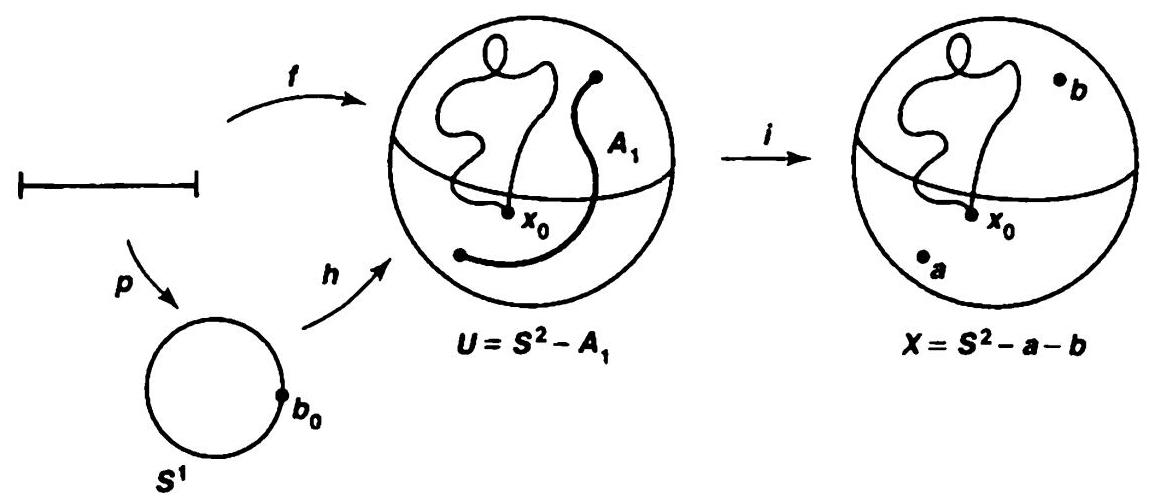
\includegraphics[width=1.0\textwidth]{images/61.3.jpg}
\end{center}
\hspace*{3em} 

Figure 61.3

Let us examine the preceding proof. What facts did we use about the simple closed curve \(C\) ? All we actually needed was the fact that \(C\) could be written as the union of the two closed connected sets \({A}_{1}\) and \({A}_{2}\) , whose intersection consisted of the two points \(a\) and \(b\) . This remark leads to the following \index{Separation theorem: closed topologist's sine curve in \({S}^{2}\)!general}\index{general separation theorem@General separation theorem}generalized version of the separation theorem, which will be useful later.
\end{proof}
\begin{theorem}[A \index{General separation theorem}]
	Let \({A}_{1}\) and \({A}_{2}\) be closed connected subsets of \({S}^{2}\) whose intersection consists of precisely two points a and \(b\) . Then the set \(C = {A}_{1} \cup  {A}_{2}\) separates \({S}^{2}\) .
\end{theorem}

\begin{proof}
	We must show first that \(C\) cannot equal all of \({S}^{2}\) . That fact was obvious in the earlier proof. In the present case, we can see that \(C \neq  {S}^{2}\) because \({S}^{2} - a - b\) is connected and \(C - a - b\) is not. (The sets \({A}_{i} - a - b\) form a separation of \(C - a - b\) .)
The remainder of the proof is a copy of the proof of the preceding theorem.
\end{proof}
\section*{Exercises}
\begin{enumerate}[itemsep=0.4em, parsep=0pt, topsep=0pt, partopsep=0pt, leftmargin=*, label=\arabic*., ref=\arabic*]
\item Give examples to show that a simple closed curve in the \index{double torus@Double torus} torus may or may not separate the torus.
\item Let \(A\) be the subset of \({\mathbb{R}}^{2}\) consisting of the union of the topologist's sine curve and the broken-line path from \(( {0, - 1})\) to \(( {0, - 2})\) to \(( {1, - 2})\) to \(( {1,\sin 1})\) . See Figure 61.4. We call \(A\) the \index{closed topologist's sine curve@Closed topologist's sine curve}closed topologist's sine curve. Show that if \(C\) is a subspace of \({S}^{2}\) homeomorphic to the closed topologist's sine curve, then \(C\) separates \({S}^{2}\) . \begin{center} 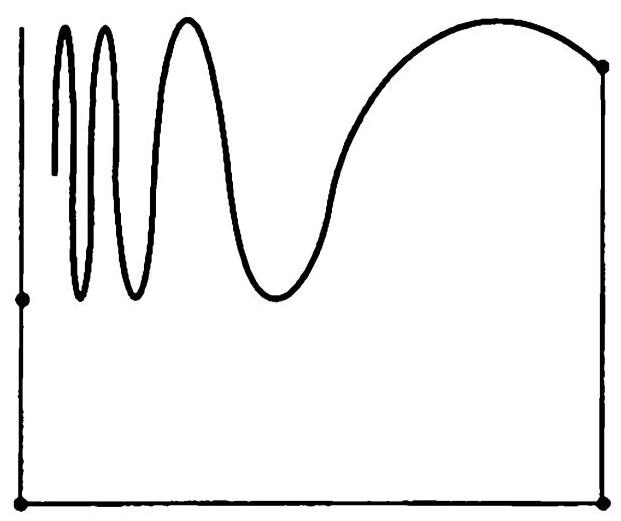
\includegraphics[width=0.5\textwidth]{images/61.4.jpg} \end{center} \hspace*{3em} Figure 61.4
\end{enumerate}
\section*{*§ 62 Invariance of Domain \protect\sectionDagger}

One of the theorems of topology that is truly fundamental, because it expresses an intrinsic property of euclidean space, is the theorem on ``\index{invariance of domain@Invariance of domain}invariance of domain,'' proved by L. E. J. Brouwer in 1912. It states that for any open set \(U\) of \({\mathbb{R}}^{n}\) and any continuous injective mapping \(f : U \rightarrow  {\mathbb{R}}^{n}\) , the image set \(f( U)\) is open in \({\mathbb{R}}^{n}\) and the inverse function is continuous. (The Inverse Function Theorem of analysis derives this result under the additional hypothesis that the map \(f\) is continuously differentiable with nonsingular Jacobian matrix.) We shall prove this theorem in the case \(n = 2\) .

\begin{lemma}[\index{homotopy extension lemma@Homotopy extension lemma}]
	Let \(X\) be a space such that \(X \times  I\) is normal. Let \(A\) be a closed subspace of \(X\) , and let \(f : A \rightarrow  Y\) be a continuous map, where \(Y\) is an open subspace of \({\mathbb{R}}^{n}\) . If \(f\) is nulhomotopic, then \(f\) may be extended to a continuous map \(g : X \rightarrow  Y\) that is also nulhomotopic.
\end{lemma}

\begin{proof}
	Let \(F : A \times  I \rightarrow  Y\) be a homotopy between \(f\) and a constant map. Then \(F( {a,0})  = f( a)\) and \(F( {a,1})  = {y}_{0}\) for all \(a\) . Extend \(F\) to the space \(X \times  1\) by setting \(F( {x,1})  = {y}_{0}\) for \(x \in  X\) Then \(F\) is a continuous map of the closed subspace \((A \times\)  \(I) \cup  ( {X \times  1})\) of \(X \times  I\) into \({\mathbb{R}}^{n}\) ; by the Tietze extension theorem, it may be extended to a continuous map \(G : X \times  I \rightarrow  {\mathbb{R}}^{n}\) .
\customfootnote{${}^{\dagger}$ In this section, we use the Tietze extension theorem ( \S 35).}

Now the map \(x \rightarrow  G( {x,0})\) is an extension of \(f\) , but it maps \(X\) into \({\mathbb{R}}^{n}\) rather than into the subspace \(Y\) To obtain our desired map, we proceed as follows: Let \(U\) be the open subset \(U = {G}^{-1}( Y)\) of \(X \times  I\) . Then \(U\) contains \(( {A \times  I})  \cup  ( {X \times  1})\) . See Figure 62.1. Since \(I\) is compact, the tube lemma implies that there is an open set \(W\) of \(X\) containing \(A\) such that \(W \times  I \subset  U\) . Now the space \(X\) is itself normal, being homeomorphic to the closed subspace \(X \times  0\) of \(X \times  I\) . Therefore, we may choose a continuous function \(\phi  : X \rightarrow  [  {0,1}]\) such that \(\phi ( x)  = 0\) for \(x \in  A\) and \(\phi ( x)  = 1\) for \(x \in  X - W\) . The map \(x \rightarrow  x \times  \phi ( x)\) carries \(X\) into the subspace \(( {W \times  I})  \cup  ( {X \times  1})\) of \(X \times  I\) , which lies in \(U\) . Then the continuous map \(g( x)  = G( {x,\phi ( x) })\) carries \(X\) into \(Y\) . And for \(x \in  A\) , we have \(\phi ( x)  = 0\) , so that \(g( x)  = G( {x,0})  = f( x)\) . Thus \(g\) is the desired extension of \(f\) . The map \(H : X \times  I \rightarrow  Y\) given by

\[
H( {x,t})  = G( {x,( {1 - t}) \phi ( x)  + t})
\]

is a homotopy between \(g\) and a constant map.

\begin{center}
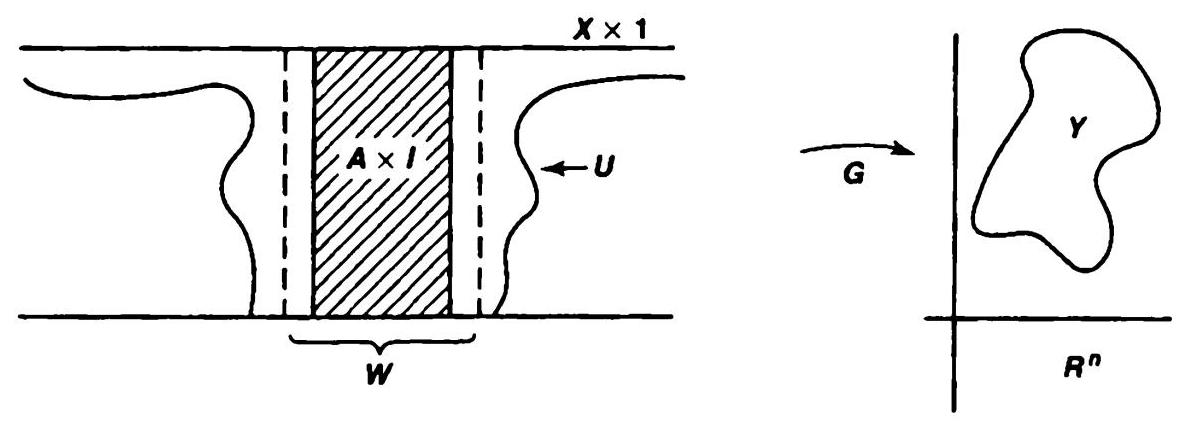
\includegraphics[width=1.0\textwidth]{images/62.1.jpg}
\end{center}
\hspace*{3em} 

Figure 62.1

The following lemma is a partial converse to the nulhomotopy lemma of the preceding section.
\end{proof}
\begin{lemma}[\index{borsuk lemma@Borsuk lemma}]
	Let \(a\) and \(b\) be points of \({S}^{2}\) . Let \(A\) be a compact space, and let \(f : A \rightarrow  {S}^{2} - a - b\) be a continuous injective map. If \(f\) is nulhomotopic, then \(a\) and \(b\) lie in the same component of \({S}^{2} - f( A)\) .
\end{lemma}

\begin{proof}
	Because \(A\) is compact and \({S}^{2}\) is Hausdorff, \(f( A)\) is a compact subspace of \({S}^{2}\) that is homeomorphic to \(A\) . Because \(f\) is nulhomotopic, so is the inclusion mapping of \(f( A)\) into \({S}^{2} - a - b\) . Hence it suffices to prove the lemma in the special case where \(f\) is simply an inclusion map. Furthermore, we can replace \({S}^{2}\) by \({\mathbb{R}}^{2} \cup  \{ \infty \}\) , letting \(a\) correspond to 0, and \(b\) to \(\infty\) . Then our lemma reduces to the following statement:
Let \(A\) be a compact subspace of \({\mathbb{R}}^{2} - \mathbf{0}\) . If the inclusion \(j : A \rightarrow  {\mathbb{R}}^{2} - \mathbf{0}\) is nulhomotopic, then0lies in the unbounded component of \({\mathbb{R}}^{2} - A\) .

This we now prove. Let \(C\) be the component of \({\mathbb{R}}^{2} - A\) containing 0; we suppose \(C\) is bounded and derive a contradiction. Let \(D\) be the union of the other components of \({\mathbb{R}}^{2} - A\) , including the unbounded component. Then \(C\) and \(D\) are disjoint open sets of \({\mathbb{R}}^{2}\) , and \({\mathbb{R}}^{2} - A = C \cup  D\) . See Figure 62.2.

We define a continuous map \(h : {\mathbb{R}}^{2} \rightarrow  {\mathbb{R}}^{2} - \mathbf{0}\) that equals the identity outside \(C\) .

Begin with the inclusion map \(j : A \rightarrow  {\mathbb{R}}^{2} - \mathbf{0}\) . Since \(j\) is by hypothesis nulho-motopic, the preceding lemma implies that \(j\) can be extended to a continuous map \(k\) of \(C \cup  A\) into \({\mathbb{R}}^{2} - \mathbf{0}\) . Then \(k\) equals the identity at points of \(A\) . Extend \(k\) to a map \(h : {\mathbb{R}}^{2} \rightarrow  {\mathbb{R}}^{2} - \mathbf{0}\) by setting \(h( x)  = x\) for \(x \in  D \cup  A\) , then \(h\) is continuous by the pasting lemma.

Now we derive a contradiction. Let \(B\) be the closed ball in \({\mathbb{R}}^{2}\) of radius \(M\) centered at the origin, where \(M\) is so large that Int \(B\) contains \(C \cup  A\) . (Here, we use the fact that \(C\) is bounded.) If we restrict \(h\) to \(B\) , we obtain a map \(g : B \rightarrow  {\mathbb{R}}^{2} - 0\) such that \(g( x)  = x\) for \(x \in  \operatorname{Bd}B\) . If we follow \(g\) by the standard retraction \(x \rightarrow  {Mx}/\parallel x\parallel\) of \({\mathbb{R}}^{2} - 0\) onto Bd \(B\) , we obtain a retraction of \(B\) onto Bd \(B\) . Such a retraction does not exist.

\begin{center}
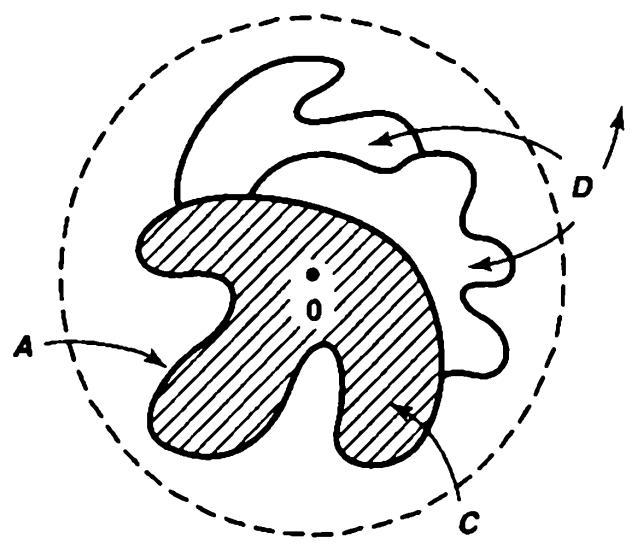
\includegraphics[width=0.5\textwidth]{images/62.2.jpg}
\end{center}
\hspace*{3em} 

Figure 62.2
\end{proof}
\begin{theorem}[Invariance of domain]
	If \(U\) is an open subset of \({\mathbb{R}}^{2}\) and \(f : U \rightarrow\)  \({\mathbb{R}}^{2}\) is continuous and injective, then \(f( U)\) is open in \({\mathbb{R}}^{2}\) and the inverse function \({f}^{-1} : f( U)  \rightarrow  U\) is continuous.
\end{theorem}

\begin{proof}
	As usual, we can replace \({\mathbb{R}}^{2}\) by \({S}^{2}\) . We show that if \(U\) is an open subset of \({\mathbb{R}}^{2}\) and \(f : U \rightarrow  {S}^{2}\) is continuous and injective, then \(f( U)\) is open in \({S}^{2}\) and the inverse function is continuous.
Step 1. We show that if \(B\) is any closed ball in \({\mathbb{R}}^{2}\) contained in \(U\) , then \(f( B)\) does not separate \({S}^{2}\) .

Let \(a\) and \(b\) be two points of \({S}^{2} - f( B)\) . Because the identity map \(i : B \rightarrow  B\) is nulhomotopic, the map \(h : B \rightarrow  {S}^{2} - a - b\) obtained by restricting \(f\) is nulhomotopic. The Borsuk lemma then implies that \(a\) and \(b\) lie in the same component of \({S}^{2} - h( B)  =\)  \({S}^{2} - f( B)\) .

Step 2. We show that if \(B\) is any closed ball of \({\mathbb{R}}^{2}\) lying in \(U\) , then \(f( {\operatorname{Int}B})\) is open in \({S}^{2}\) .

The space \(C = f( {\operatorname{Bd}B})\) is a simple closed curve in \({S}^{2}\) , so it separates \({S}^{2}\) . Let \(V\) be the component of \({S}^{2} - C\) that contains the connected set \(f( {\operatorname{Int}B})\) , and let \(W\) be the union of the others. Because \({S}^{2}\) is locally connected, \(V\) and \(W\) are open in \({S}^{2}\) . We show \(V = f( {\operatorname{Int}B})\) , and we are through.

We suppose \(a\) is a point of \(V\) that is not in \(f( {\operatorname{Int}B})\) and derive a contradiction. Let \(b\) be a point of \(W\) . Since the set \(D = f( B)\) does not separate \({S}^{2}\) , the set \({S}^{2} - D\) is a connected set containing \(a\) and \(b\) . This set is contained in \({S}^{2} - C\) (since \(D \supset  C\) ); it follows that \(a\) and \(b\) lie in the same component of \({S}^{2} - C\) , contrary to construction. See Figure 62.3.

\begin{center}
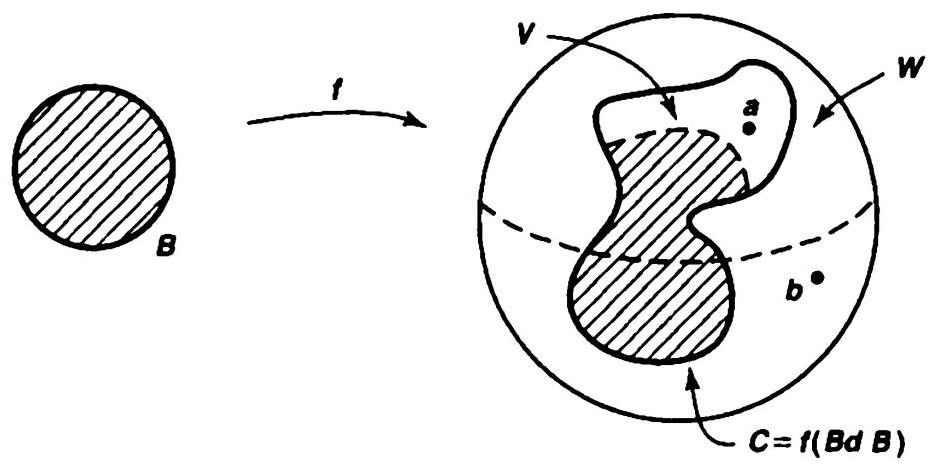
\includegraphics[width=0.8\textwidth]{images/62.3.jpg}
\end{center}
\hspace*{3em} 

Figure 62.3

Step 3. We prove the theorem. Since, for any ball \(B\) contained in \(U\) , the set \(f( {\text{ Int }B})\) is open in \({S}^{2}\) , the map \(f : U \rightarrow  {S}^{2}\) is an open map. It follows that \(f( U)\) is open in \({S}^{2}\) and \({f}^{-1}\) is continuous.
\end{proof}
\section*{Exercises}
\begin{enumerate}[itemsep=0.4em, parsep=0pt, topsep=0pt, partopsep=0pt, leftmargin=*, label=\arabic*., ref=\arabic*]
\item Give an example to show that the conclusion of the Borsuk lemma need not hold if \(f\) is not injective.
\item Let \(A\) be a compact contractible subspace of \({S}^{2}\) . Show that \(A\) does not separate \({S}^{2}\) .
\item Let \(X\) be a space such that \(X \times  I\) is normal. Let \(A\) be a closed subspace of \(X\) ; let \(f : A \rightarrow  Y\) be a continuous map, where \(Y\) is an open subspace of \({\mathbb{R}}^{n}\) . If \(f\) is homotopic to a map that is extendable to a continuous map \(h : X \rightarrow  Y\) , then \(f\) itself is extendable to a continuous map \(g : X \rightarrow  Y\) , such that \(g \simeq  h\) .
\item Let \(C\) be a simple closed curve in \({\mathbb{R}}^{2} - 0\) ; let \(j : C \rightarrow  {\mathbb{R}}^{2} - 0\) be the inclusion mapping. Show that \({j}_{ * }\) is trivial if 0 lies in the unbounded component of \({\mathbb{R}}^{2} - C\) , and is nontrivial otherwise. (In fact, \({j}_{ * }\) is an isomorphism in the latter case, as we shall prove in  \S 65.)
\item Theorem. Let \(U\) be a simply connected open set in \({\mathbb{R}}^{2}\) . If \(C\) is a simple closed curve lying in \(U\) , then each bounded component of \({\mathbb{R}}^{2} - C\) also lies in \(U\) . (This condition actually characterizes the simply connected open sets of \({\mathbb{R}}^{2}\) . See \cite{Rudin1987}. The space \({\mathbb{R}}^{2} - C\) has, of course, only one bounded component, as we shall prove in the next section.)
\item Suppose you are given that there is no retraction of \({B}^{n}\) onto \({S}^{n - 1}\) .
  \begin{enumerate}[itemsep=0.2em, parsep=0pt, topsep=0pt, partopsep=0pt, leftmargin=*, label=(\alph*), align=left]
  \item Show the Borsuk lemma holds for \({S}^{n}\) .
  \item Show that no compact contractible subspace of \({S}^{n}\) separates \({S}^{n}\) .
  \item Suppose you are given also that any subspace of \({S}^{n}\) homeomorphic to \({S}^{n - 1}\) separates \({S}^{n}\) . Prove the invariance of domain theorem in dimension \(n\) .
  \end{enumerate}
\end{enumerate}
\section*{§ 63 The Jordan Curve Theorem}

The special case of the Seifert-van Kampen theorem that we used in proving the Jordan separation theorem tells us something about the fundamental group of the space \(X =\)  \(U \cup  V\) in the case where the intersection \(U \cap  V\) is path connected. In the next theorem, we examine what happens when \(U \cap  V\) is not path connected. This result will enable us to complete the proof of the Jordan curve theorem.

\begin{theorem}
	Let \(X\) be the union of two open sets \(U\) and \(V\) , such that \(U \cap  V\) can be written as the union of two disjoint open sets \(A\) and \(B\) . Assume that there is a path \(\alpha\) in \(U\) from a point \(a\) of \(A\) to a point \(b\) of \(B\) , and that there is a path \(\beta\) in \(V\) from \(b\) to \(a\) . Let \(f\) be the loop \(f = \alpha  * \beta\) .

(a) The path-homotopy class \([  f]\) generates an infinite cyclic subgroup of \({\pi }_{1}( {X,a})\) .

*(b) If \({\pi }_{1}( {X,a})\) is itself infinite cyclic, it is generated by \([  f]  {.}^{\dagger}\)

(c) Assume there is a path \(\gamma\) in \(U\) from a to the point \({a}^{\prime }\) of \(A\) , and that there is a path \(\delta\) in \(V\) from \({a}^{\prime }\) to \(a\) . Let \(g\) be the loop \(g = \gamma  * \delta\) . Then the subgroups of \({\pi }_{1}( {X,a})\) generated by \([  f]\) and \([  g]\) intersect in the identity element alone.
\end{theorem}

\begin{proof}
	The proof is in many ways an imitation of the proof in  \S 54 that the fundamental group of the circle is infinite cyclic. As in that proof, the crucial step is to find an appropriate covering space \(E\) for the space \(X\) .
Step 1. (Construction of \(E\) ). We construct \(E\) by pasting together copies of the subspaces \(U\) and \(V\) . Let us take countably many copies of \(U\) and countably many copies of \(V\) , all disjoint, say

\[
U \times  ( {2n}) \;\text{ and }\;V \times  ( {{2n} + 1})
\]

for all \(n \in  \mathbb{Z}\) , where \(\mathbb{Z}\) denotes the integers. Let \(Y\) denote the union of these spaces; \(Y\) is a subspace of \(X \times  \mathbb{Z}\) . Now we form a new space \(E\) as a quotient space of \(Y\) by identifying the points

\[
x \times  ( {2n}) \;\text{ and }\;x \times  ( {{2n} - 1}) \;\text{ for }x \in  A
\]

\customfootnote{${}^{\dagger}$ This result uses Theorem 54.6, and will be used only when we deal with \index{Simple closed curve!winding number}winding numbers in \S 65.}

and by identifying the points

\[
x \times  ( {2n}) \;\text{ and }\;x \times  ( {{2n} + 1}) \;\text{ for }x \in  B.
\]

Let \(\pi  : Y \rightarrow  E\) be the quotient map.

Now the map \(\rho  : Y \rightarrow  X\) defined by \(\rho ( {x \times  m})  = x\) induces a map \(p : E \rightarrow  X\) ; the map \(p\) is continuous because \(E\) has the quotient topology. The map \(p\) is also surjective. We shall show that \(p\) is a covernng map. See Figure 63.1.

First let us show that the map \(\pi\) is an open map. Since \(Y\) is the union of the disjoint open sets \(\{ U \times  ( {2n}) \}\) and \(\{ V \times  ( {{2n} + 1}) \}\) , it will suffice to show that \(\pi  \mid  ( {U \times  {2n}})\) and \(\pi  \mid  ( {V \times  ( {{2n} + 1}) })\) are open maps. And this is easy. Take an open set in \(U \times  {2n}\) , for example; it will be of the form \(W \times  {2n}\) , where \(W\) is open in \(U\) . Then

\[
{\pi }^{-1}( {\pi ( {W \times  {2n}}) })  = [  {W \times  {2n}}] \cup  [  {( {W \cap  B})  \times  ( {{2n} + 1}) }]
\]

\[
\cup  [  {( {W \cap  A})  \times  ( {{2n} - 1}) }]  \text{ , }
\]

which is the union of three open sets of \(Y\) and hence open in \(Y\) . By definition of the quotient topology, \(\pi ( {W \times  {2n}})\) is open in \(E\) , as desired.

Now we prove that \(p\) is a covering map; we show that the open sets \(U\) and \(V\) are evenly covered by \(p\) . Consider \(U\) , for example. The set \({p}^{-1}( U)\) is the union of the disjoint sets \(\pi ( {U \times  {2n}})\) for \(n \in  \mathbb{Z}\) . Each of these sets is open in \(E\) because \(\pi\) is an open map. Let \({\pi }_{2n}\) denote the restriction of \(\pi\) to the open set \(U \times  {2n}\) , mapping it onto \(\pi ( {U \times  {2n}})\) . It is a homeomorphism because it is bijective, continuous, and open. Then when restricted to \(\pi ( {U \times  {2n}})\) , the map \(p\) is just the composite of the two homeomorphisms

\[
\pi ( {U \times  {2n}}) \xrightarrow[]{{\pi }_{2n}^{-1}}U \times  {2n}\overset{\rho }{ \rightarrow  }U
\]

and is thus a homeomorphism. Therefore, \(p \mid  \pi ( {U \times  {2n}})\) maps this set homeomorphi-cally onto \(U\) , as desired.

Step 2. Now we define a family of liftings of the loop \(f = \alpha  * \beta\) .

For each integer \(n\) , let \({e}_{n}\) be the point \(\pi ( {a \times  {2n}})\) of \(E\) . Then the points \({e}_{n}\) are distinct, and they constitute the set \({p}^{-1}( a)\) . We define a lifting \({\widetilde{f}}_{n}\) of \(f\) that begins at \({e}_{n}\) and ends at \({e}_{n + 1}\) .

Since \(\alpha\) and \(\beta\) are paths in \(U\) and \(V\) , respectively, we can define

\[
\begin{aligned}  & {\bar{\alpha }}_{n}( s)  = \pi ( {\alpha ( s)  \times  {2n}}) , \\  & {\widetilde{\beta }}_{n}( s)  = \pi ( {\beta ( s)  \times  ( {{2n} + 1}) }) ; \end{aligned}
\]

then \({\widetilde{\alpha }}_{n}\) and \({\widetilde{\beta }}_{n}\) are liftings of \(\alpha\) and \(\beta\) , respectively. (The case \(n = 0\) is illustrated in Figure 63.1 ) The product \({\widetilde{\alpha }}_{n} * {\widetilde{\beta }}_{n}\) is defined, since \({\widetilde{\alpha }}_{n}\) ends at \(\pi ( {b \times  {2n}})\) and \({\widetilde{\beta }}_{n}\) begins at \(\pi ( {b \times  ( {{2n} + 1}) })\) . We set \({\widetilde{f}}_{n} = {\widetilde{\alpha }}_{n} * {\widetilde{\beta }}_{n}\) , and note that \({\widetilde{f}}_{n}\) begins at \({\widetilde{\alpha }}_{n}( 0)  = \pi ( {a \times  {2n}})  = {e}_{n}\) and ends at \({\bar{\beta }}_{n}( 1)  = \pi ( {a \times  ( {{2n} + 1}) })  = \pi ( {a \times  ( {{2n} + 2}) })  = {e}_{n + 1}\) .

\begin{center}
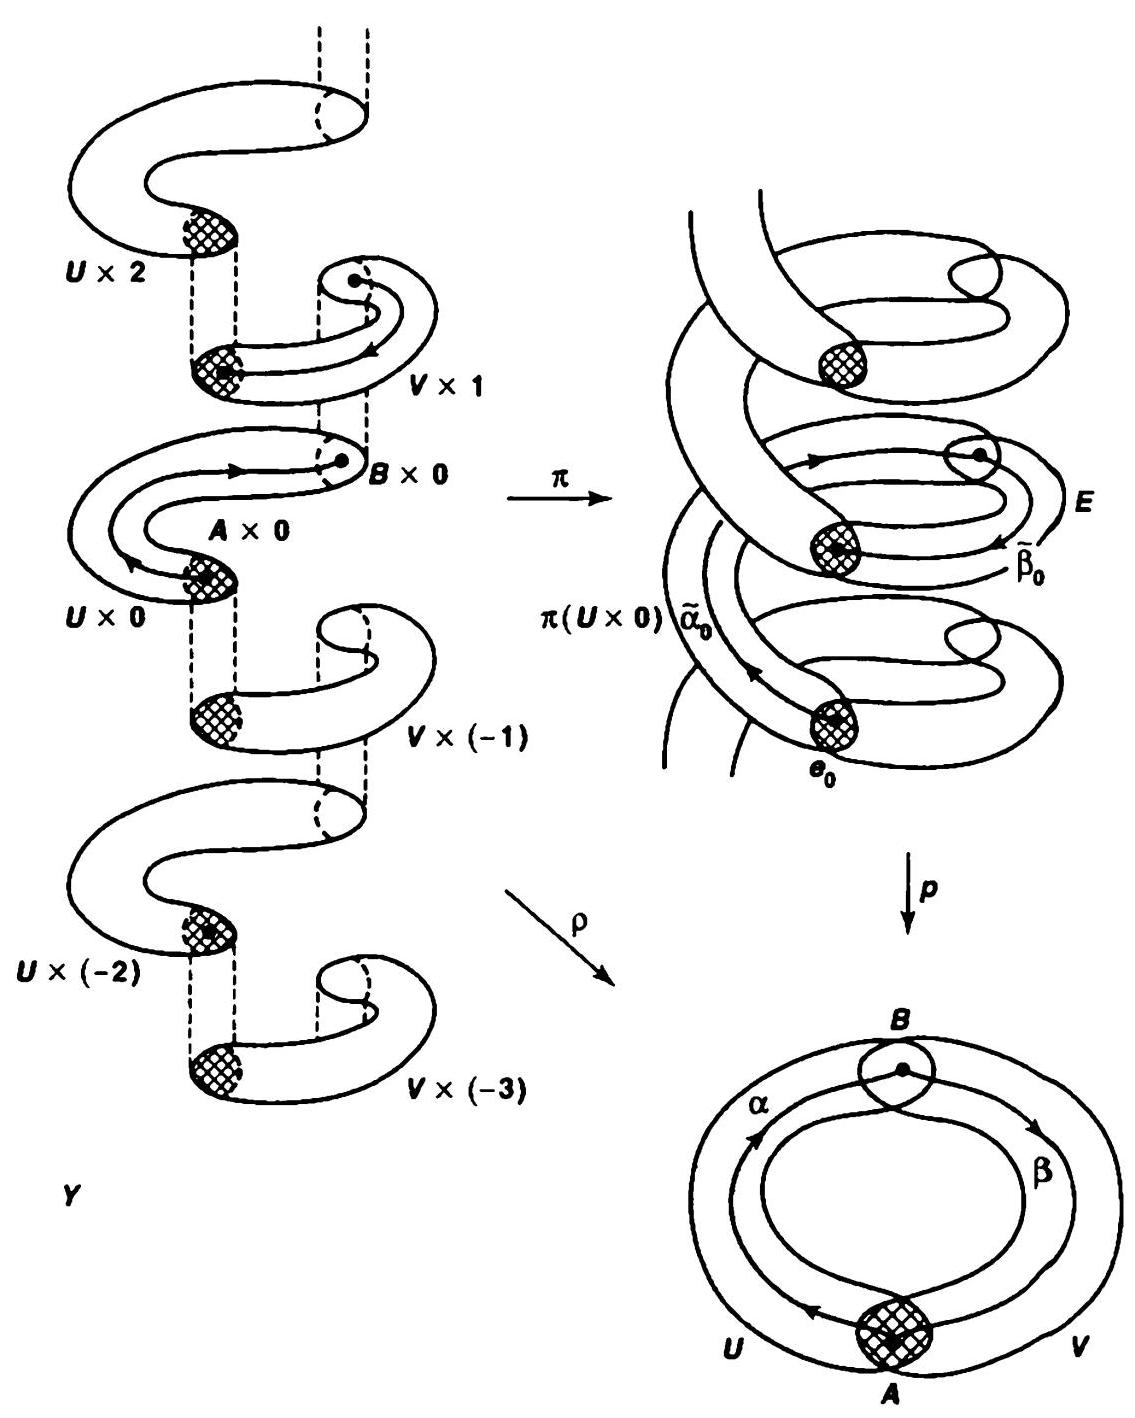
\includegraphics[width=1.0\textwidth]{images/63.1.jpg}
\end{center}
\hspace*{3em} 

Figure 63.1

Step 3. We show that \([  f]\) generates an infinite cyclic subgroup of \({\pi }_{1}( {X,a})\) . It suffices to show that if \(m\) is a positive integer, then \({[  f]  }^{m}\) is not the identity element. But this is easy. For the product

\[
\widetilde{h} = {\bar{f}}_{0} * ( {{\bar{f}}_{1} * ( {\cdots  * {\bar{f}}_{m - 1}}) })
\]

is defined and is a lifting of the \(m\) -fold product

\[
h = f * ( {f * ( {\cdots  * f}) }) .
\]

Because \(\bar{h}\) begins at \({e}_{0}\) and ends at \({e}_{m}\) , the class \([  h] = {[  f]  }^{m}\) cannot be trivial.

*Step 4. Now we show that if \({\pi }_{1}( {X,a})\) is infinite cyclic, it is generated by \([  f]\) . Consider the lifting correspondence \(\phi  : {\pi }_{1}( {X,a})  \rightarrow  {p}^{-1}( a)\) . We showed in Step 3 that for each positive integer \(m\) , the correspondence \(\phi\) carries \({[  f]  }^{m}\) to the point \({e}_{m}\) of \({p}^{-1}( a)\) . A similar argument shows that it carries \({[  f]  }^{-m}\) to \({e}_{-m}\) . Thus \(\phi\) is surjective. Now by Theorem 54.6, \(\phi\) induces an injective map

\[
\Phi  : {\pi }_{1}( {X,a}) /H \rightarrow  {p}^{-1}( a)
\]

where \(H = {p}_{ * }( {{\pi }_{1}( {E,{e}_{0}}) })\) ; the map \(\Phi\) is surjective because \(\phi\) is surjective. It follows that \(H\) is the trivial group, since the quotient of an infinite cyclic group by any nontrivial subgroup is finite. Then the lifting correspondence \(\phi\) itself is bijective; since it maps the subgroup generated by \([  f]\) onto \({p}^{-1}( a)\) , this subgroup must equal all of \({\pi }_{1}( {X,a})\) .

Step 5. Now we prove (c). The picture in Figure 63.1 may mislead you into thinking that the element \([  g]\) of \({\pi }_{1}( {X,a})\) considered in part (c) is in fact trivial. But that figure is rather special. Figure 63.2 illustrates what can occur when \(A\) is itself the union of two disjoint nonempty open sets. In this case (which will be useful to us shortly) both \([  f]\) and \([  g]\) generate infinite cyclic subgroups of \({\pi }_{1}( {X,a})\) .

\begin{center}
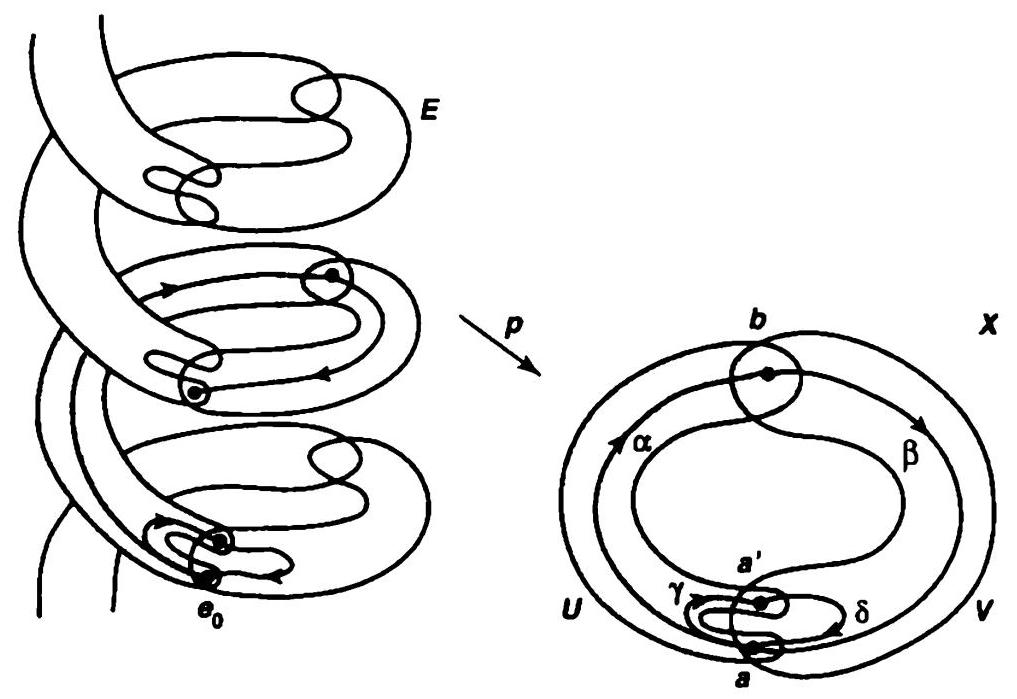
\includegraphics[width=0.9\textwidth]{images/63.2.jpg}
\end{center}
\hspace*{3em} 

Figure 63.2

Given \(g = \gamma  * \delta\) , we define a lifting of \(g\) to \(E\) as follows: Since \(\gamma\) is a path in \(U\) , we can define

\[
\widetilde{\gamma }( s)  = \pi ( {\gamma ( s)  \times  0}) ;
\]

since \(\delta\) is a path in \(V\) , we can define

\[
\widetilde{\delta }( s)  = \pi ( {\delta ( s)  \times  ( {-1}) }) .
\]

Then \(\widetilde{\gamma }\) and \(\widetilde{\delta }\) are liftings of \(\gamma\) and \(\delta\) . The product \(\bar{g} = \widetilde{\gamma } * \widetilde{\delta }\) is defined, since \(\widetilde{\gamma }\) ends at \(\pi ( {{a}^{\prime } \times  0})\) and \(\widetilde{\delta }\) begins at \(\pi ( {{a}^{\prime } \times  ( {-1}) })\) ; and it is a lifting of \(g\) . Note that \(\bar{g}\) is a loop in \(E\) , for it begins and ends at \(\pi ( {a \times  0})  = \pi ( {a \times  ( {-1}) })  = {e}_{0}\) .

It follows that the subgroups generated by \([  f]\) and \([  g]\) have only the identity element in common. For the \(m\) -fold product of \(f\) with itself lifts to a path that begins at \({e}_{0}\) and ends at \({e}_{m}\) , while every product of \(g\) with itself lifts to a path beginning and ending at \({e}_{0}\) . Hence \({[  f]  }^{m} \neq  {[  g]  }^{k}\) for every nonzero \(m\) and \(k\) .
\end{proof}
\begin{theorem}[A nonseparation theorem]
	Let \(D\) be an arc in \({S}^{2}\) . Then \(D\) \index{Arc!does not separate \({S}^{2}\)}does not separate \({S}^{2}\) .
\end{theorem}

\begin{proof}
	We give two proofs of this theorem. The first uses the results of the preceding section, and the second does not.
First proof. Because \(D\) is contractible, the identity map i : \(D \rightarrow  D\) is nulhomo-topic. Hence if \(a\) and \(b\) are any two points of \({S}^{2}\) not in \(D\) , the inclusion \(j : D \rightarrow\)  \({S}^{2} - a - b\) is nulhomotopic. The \index{borsuk lemma@Borsuk lemma}Borsuk lemma then implies that \(a\) and \(b\) lie in the same component of \({S}^{2} - D\) .

Second Proof. Let us write \(D\) as the union of two arcs \({D}_{1}\) and \({D}_{2}\) that intersect in a single point \(d\) . Let \(a\) and \(b\) be points not in \(D\) . We show that if \(a\) and \(b\) can be joined by paths in \({S}^{2} - {D}_{1}\) and in \({S}^{2} - {D}_{2}\) , then they can be joined by a path in \({S}^{2} - D\) . Figure 63.3 illustrates the fact that this assertion is not entirely trivial.

\begin{center}
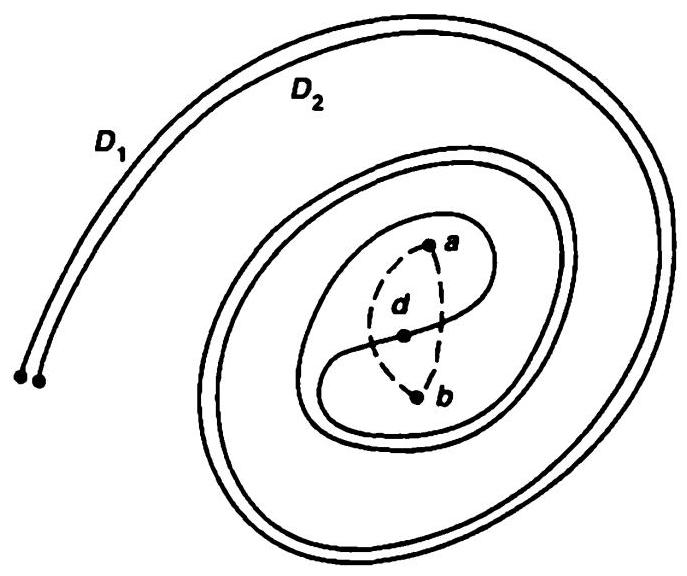
\includegraphics[width=0.6\textwidth]{images/63.3.jpg}
\end{center}
\hspace*{3em} 

Figure 63.3

We suppose that \(a\) and \(b\) cannot be joined by a path in \({S}^{2} - D\) and derive a contradiction. We apply Theorem 63.1. Let \(X\) be the space \({S}^{2} - d\) . Let \(U\) and \(V\) be the open sets

\[
U = {S}^{2} - {D}_{1}\;\text{ and }\;V = {S}^{2} - {D}_{2}.
\]

Then \(X = U \cup  V\) , and \(U \cap  V = {S}^{2} - D\) . By hypothesis, \(a\) and \(b\) are points of \({S}^{2} - D\) that cannot be joined by a path in \({S}^{2} - D\) . Therefore, \(U \cap  V\) is not path connected. Let \(A\) be the path component of \(U \cap  V\) containing \(a\) ; let \(B\) be the union of the other path components of \(U \cap  V\) . Since \(U \cap  V\) is locally path connected (being open in \({S}^{2}\) ), the path components of \(U \cap  V\) are open; hence \(A\) and \(B\) are open in \(X\) . We are given that \(a\) and \(b\) can be joined by paths in \(U = {S}^{2} - {D}_{1}\) and \(V = {S}^{2} - {D}_{2}\) . We conclude from Theorem 63.1 that \({\pi }_{1}( {X,a})\) is not trivial. But \(X = {S}^{2} - d\) , so its fundamental group is trivial.

Now we prove the theorem Given the arc \(D\) and the points \(a\) and \(b\) of \({S}^{2} - D\) , we suppose that \(a\) and \(b\) cannot be joined by a path in \({S}^{2} - D\) and derive a contradiction. Choose a homeomorphism \(h : [  {0,1}] \rightarrow  D\) ; let \({D}_{1} = h( [  {0,1/2}]  )\) and \({D}_{2} = h( [  {1/2,1}]  )\) . The result of the preceding paragraph shows that since \(a\) and \(b\) cannot be joined by a path in \({S}^{2} - D\) , they cannot be joined by paths in both \({S}^{2} - {D}_{1}\) and \({S}^{2} - {D}_{2}\) . To be definite, suppose that \(a\) and \(b\) cannot be joined by a path in \({S}^{2} - {D}_{1}\) .

Now repeat the argument, breaking \({D}_{1}\) up into two arcs \({E}_{1} = h( [  {0,1/4}]  )\) and \({E}_{2} = h( [  {1/4,1/2}]  )\) . We conclude, as before, that \(a\) and \(b\) cannot be joined by paths in both \({S}^{2} - {E}_{1}\) and \({S}^{2} - {E}_{2}\)

Contune similarly. In this way we define a sequence

\[
I \supset  {I}_{1} \supset  {I}_{2} \supset  \cdots
\]

of closed intervals such that \({I}_{n}\) has length \({( 1/2) }^{n}\) and such that for each \(n\) , the points \(a\) and \(b\) cannot be joined by a path in \({S}^{2} - h( {I}_{n})\) . Compactness of the unit interval guarantees there is a point \(x\) in \(\bigcap {I}_{n}\) ; since the lengths of the intervals converge to zero, there is only one such point.

Consider the space \({S}^{2} - h( x)\) . Since this space is homeomorphic to \({\mathbb{R}}^{2}\) , the points \(a\) and \(b\) can be joined by a path \(\alpha\) in \({S}^{2} - h( x)\) . Because \(\alpha ( I)\) is compact, it is closed, so some \(\epsilon\) -neighborhood of \(h( x)\) is disjoint from \(\alpha ( I)\) . Then because \(h\) is continuous, there is some \(m\) such that \(h( {I}_{m})\) lies in this \(\epsilon\) -neighborhood. It follows that \(\alpha\) is a path in \({S}^{2} - h( {I}_{m})\) joining \(a\) and \(b\) , contrary to hypothesis.

Both proofs of this theorem are interesting. As we noted in  \S 62, the first generalizes to show that no compact contractible subspace of \({S}^{2}\) separates \({S}^{2}\) . The second generalizes in another direction. Let us examine this second proof, and ask ourselves what properties of the sets \({D}_{1}\) and \({D}_{2}\) made it work? One readily sees that all that was needed was the fact that \({D}_{1}\) and \({D}_{2}\) were closed subsets of \({S}^{2}\) and that \({S}^{2} - ( {{D}_{1} \cap  {D}_{2}})\) was simply connected. Hence we have the following result, which we shall use later:
\end{proof}
\begin{theorem}[A \index{General nonseparation theorem}]
	Let \({D}_{1}\) and \({D}_{2}\) be closed subsets of \({S}^{2}\) such that \({S}^{2} - {D}_{1} \cap  {D}_{2}\) is simply connected. If neither \({D}_{1}\) nor \({D}_{2}\) separates \({S}^{2}\) , then \({D}_{1} \cup  {D}_{2}\) does not separate \({S}^{2}\) .
\end{theorem}

Now we prove the Jordan curve theorem.

\begin{theorem}[The Jordan curve theorem]
	Let \(C\) be a simple closed curve in \({S}^{2}\) . Then \(C\) separates \({S}^{2}\) into precisely two components \({W}_{1}\) and \({W}_{2}\) . Each of the sets \({W}_{1}\) and \({W}_{2}\) has \(C\) as its boundary; that is, \(C = {\bar{W}}_{i} - {W}_{i}\) for \(\mathrm{i} = 1,2\) .
\end{theorem}

\begin{proof}
	Step 1. We first prove that \({S}^{2} - C\) has precisely two components. Write \(C\) as the union of two arcs \({C}_{1}\) and \({C}_{2}\) that intersect in a two-point set \(\{ p,q\}\) . Let \(X\) be the space \({S}^{2} - p - q\) , and let \(U\) and \(V\) be the open sets
\[
U = {S}^{2} - {C}_{1}\;\text{ and }\;V = {S}^{2} - {C}_{2}.
\]

Then \(X = U \cup  V\) , and \(U \cap  V = {S}^{2} - C\) . The space \(U \cap  V\) has at least two components, by the Jordan separation theorem.

We suppose that \(U \cap  V\) has more than two components and derive a contradiction. Let \({A}_{1}\) and \({A}_{2}\) be two of the components of \(U \cap  V\) , and let \(B\) be the union of the others. Because \({S}^{2} - C\) is locally connected, each of these sets is open. Let \(a \in  {A}_{1}\) and \({a}^{\prime } \in  {A}_{2}\) and \(b \in  B\) . Because the arcs \({C}_{1}\) and \({C}_{2}\) do not separate \({S}^{2}\) , there are paths \(\alpha\) and \(\gamma\) in \(U\) from \(a\) to \(b\) and from \(a\) to \({a}^{\prime }\) , respectively, and there are paths \(\beta\) and \(\delta\) in \(V\) from \(b\) to \(a\) and from \({a}^{\prime }\) to \(a\) , respectively. Consider the loops \(f = \alpha  * \beta\) and \(g = \gamma  * \delta\) . Writing \(U \cap  V\) as the union of the open sets \({A}_{1} \cup  {A}_{2}\) and \(B\) , we see that Theorem 63.1 implies that \([  f]\) is a nontrivial element of \({\pi }_{1}( {X,a})\) . Writing \(U \cap  V\) as the union of the disjoint open sets \({A}_{1}\) and \({A}_{2} \cup  B\) , we see that \([  g]\) is also a nontrivial element of \({\pi }_{1}( {X,a})\) . Since \({\pi }_{1}( {X,a})\) is infinite cyclic, we must have \({[  f]  }^{m} = {[  g]  }^{k}\) for some nonzero integers \(m\) and \(k\) . This result contradicts (c) of Theorem 63.1 .

Step 2. Now we show that \(C\) is the common boundary of \({W}_{1}\) and \({W}_{2}\)

Because \({S}^{2}\) is locally connected, each of the components \({W}_{1}\) and \({W}_{2}\) of \({S}^{2} - C\) is open in \({S}^{2}\) . In particular, neither contains a limit point of the other, so that both the sets \({\bar{W}}_{1} - {W}_{1}\) and \({\bar{W}}_{2} - {W}_{2}\) must be contained in \(C\) .

To prove the reverse inclusion, we show that if \(x\) is a point of \(C\) , every neighborhood \(U\) of \(x\) intersects the closed set \({\bar{W}}_{1} - {W}_{1}\) . It follows that \(x\) is in the set \({\bar{W}}_{1} - {W}_{1}\) .

So let \(U\) be a neighborhood of \(x\) . Because \(C\) is homeomorphic to the circle \({S}^{1}\) , we can break \(C\) up into two arcs \({C}_{1}\) and \({C}_{2}\) that intersect in only their end points, such that \({C}_{1}\) is small enough that it lies inside \(U\) . See Figure 63.4.

\begin{center}
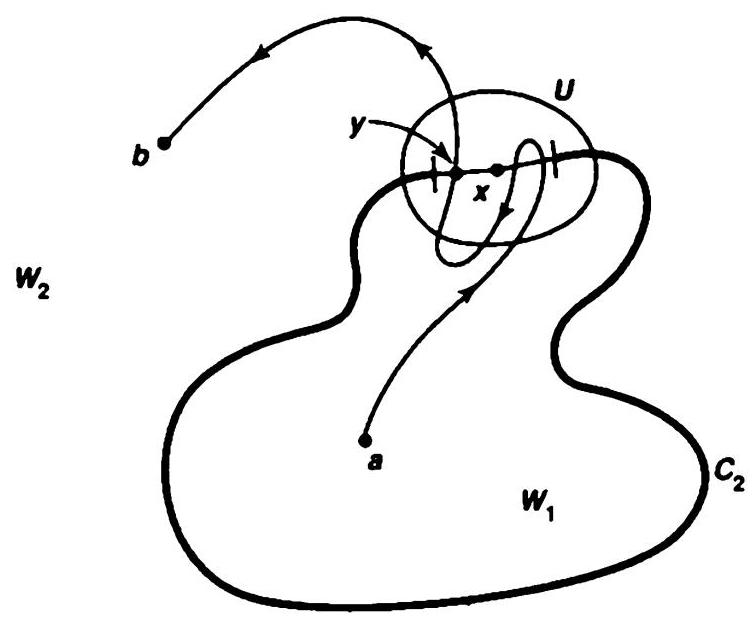
\includegraphics[width=0.7\textwidth]{images/63.4.jpg}
\end{center}
\hspace*{3em} 

Figure 63.4

Let \(a\) and \(b\) be points of \({W}_{1}\) and \({W}_{2}\) , respectively. Because \({C}_{2}\) does not separate \({S}^{2}\) , we can find a path \(\alpha\) in \({S}^{2} - {C}_{2}\) joining \(a\) and \(b\) . The set \(\alpha ( I)\) must contain a point \(y\) of the set \({\bar{W}}_{1} - {W}_{1}\) , because otherwise \(\alpha ( I)\) would be a connected set lying in the union of the disjoint open sets \({W}_{1}\) and \({S}^{2} - {\bar{W}}_{1}\) , and intersecting each of them. The point \(y\) belongs to the closed curve \(C\) , since \(( {{\bar{W}}_{1} - {W}_{1}})  \subset  C\) . Because the path \(\alpha\) does not intersect the arc \({C}_{2}\) , the point \(y\) must therefore lie in the arc \({C}_{1}\) , which in turn lies in the open set \(U\) . Thus, \(U\) intersects \({\bar{W}}_{1} - {W}_{1}\) in the point \(y\) , as desired.

Just as with the earlier theorems, we now ask ourselves what made the proof of this theorem work. Examining Step 1 of the proof, we see that all we used were the facts that \({C}_{1}\) and \({C}_{2}\) were closed connected sets, that \({C}_{1} \cap  {C}_{2}\) consisted of two points, and that neither \({C}_{1}\) nor \({C}_{2}\) separated \({S}^{2}\) . The first two facts implied that \({C}_{1} \cup  {C}_{2}\) separated \({S}^{2}\) into at least two components; the third implied that there were only two components. Hence one has, with no further effort, the following result:
\end{proof}
\begin{theorem}
	Let \({C}_{1}\) and \({C}_{2}\) be closed connected subsets of \({S}^{2}\) whose intersection consists of two points. If neither \({C}_{1}\) nor \({C}_{2}\) separates \({S}^{2}\) , then \({C}_{1} \cup  {C}_{2}\) separates \({S}^{2}\) into precisely two components.
\end{theorem}

Example 1. The second half of the Jordan curve theorem, to the effect that \(C\) is the common boundary of \({W}_{1}\) and \({W}_{2}\) , may seem so obvious as hardly to require comment. But it depends crucially on the fact that \(C\) is homeomorphic to \({S}^{1}\) .

For instance, consider the space indicated in Figure 63 5. It is the union of two arcs whose intersection consists of two points, so it separates \({S}^{2}\) into two components \({W}_{1}\) and \({W}_{2}\) just as the circle does, by Theorem 63.5. But \(C\) does not equal the common boundary of \({W}_{1}\) and \({W}_{2}\) in this case.

\begin{center}
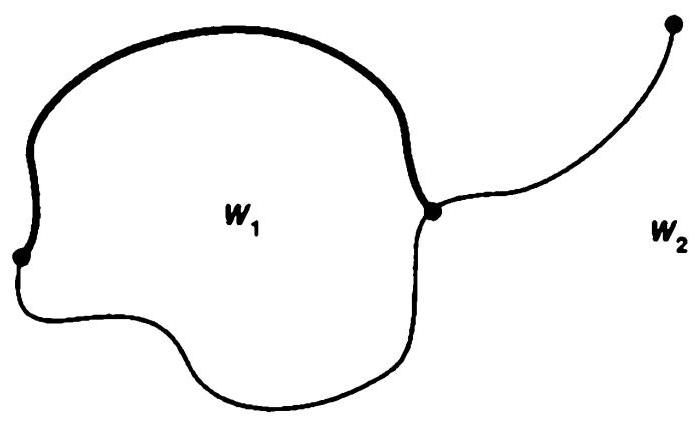
\includegraphics[width=0.6\textwidth]{images/63.5.jpg}
\end{center}
\hspace*{3em} 

Figure 63.5

There is a fourth theorem that is often considered along with these three separation theorems. It is called the \index{schoenflies theorem@Schoenflies theorem}, and it states that if \(C\) is a simple closed curve in \({S}^{2}\) and \(U\) and \(V\) are the components of \({S}^{2} - C\) , then \(\bar{U}\) and \(\bar{V}\) are each homeomorphic to the closed unit ball \({B}^{2}\) . A proof may be found in 		\cite{HallSpencer1955}.

The separation theorems can be generalized to higher dimensions as follows: (1) Any subspace \(C\) of \({S}^{n}\) homeomorphic to \({S}^{n - 1}\) separates \({S}^{n}\) .

(2) No subspace \(A\) of \({S}^{n}\) homeomorphic to \([  {0,1}]\) or to some ball \({B}^{m}\) separates \({S}^{n}\) .

(3) Any subspace \(C\) of \({S}^{n}\) homeomorphic to \({S}^{n - 1}\) separates \({S}^{n}\) into two components, of which \(C\) is the common boundary.

These theorems can be proved quite readily once one has studied singular homology groups in algebraic topology. (See 		\cite{Munkres1993}, p. 202.) The Brouwer theorem on invariance of domain for \({\mathbb{R}}^{n}\) follows as a corollary.

The \index{schoenflies theorem@Schoenflies theorem}Schoenflies theorem, however, does not generalize to higher dimensions without some restrictions on the way the space \(C\) is imbedded in \({S}^{n}\) . This is shown by the famous example of the ``\index{alexander horned sphere@Alexander horned sphere},'' a homeomorphic image of \({S}^{2}\) in \({S}^{3}\) , one of whose complementary domains is not simply connected! (See 		\cite{HockingYoung1961}, p. 176.)

The separation theorems can be generalized even further than this. The definitive theorem along these lines is the famous Alexander-Pontryagin duality theorem, a rather deep theorem of algebraic topology, which we shall not attempt to state here. (See 		\cite{Munkres1993}.) It implies that if the closed subspace \(C\) separates \({S}^{n}\) into \(k\) components, so does any subspace of \({S}^{n}\) that is homeomorphic to \(C\) (or even homotopy equivalent to \(C\) ). The separation theorems (1)-(3) are immediate corollaries.

\section*{Exercises}
\begin{enumerate}[itemsep=0.4em, parsep=0pt, topsep=0pt, partopsep=0pt, leftmargin=*, label=\arabic*., ref=\arabic*]
\item Let \({C}_{1}\) and \({C}_{2}\) be disjoint simple closed curves in \({S}^{2}\) .
  \begin{enumerate}[itemsep=0.2em, parsep=0pt, topsep=0pt, partopsep=0pt, leftmargin=*, label=(\alph*), align=left]
  \item Show that \({S}^{2} - {C}_{1} - {C}_{2}\) has precisely three components. [Hint: If \({W}_{1}\) is the component of \({S}^{2} - {C}_{1}\) disjoint from \({C}_{2}\) , and if \({W}_{2}\) is the component of \({S}^{2} - {C}_{2}\) disjoint from \({C}_{1}\) , show that \({\bar{W}}_{1} \cup  {\bar{W}}_{2}\) does not separate \({S}^{2}\) .]
  \item Show that these three components have boundaries \({C}_{1}\) and \({C}_{2}\) and \({C}_{1} \cup  {C}_{2}\) , respectively.
  \end{enumerate}
\item Let \(D\) be a closed connected subspace of \({S}^{2}\) that separates \({S}^{2}\) into \(n\) components.
  \begin{enumerate}[itemsep=0.2em, parsep=0pt, topsep=0pt, partopsep=0pt, leftmargin=*, label=(\alph*), align=left]
  \item If \(A\) is an arc in \({S}^{2}\) whose intersection with \(D\) consists of one of its end points, show that \(D \cup  A\) separates \({S}^{2}\) into \(n\) components.
  \item If \(A\) is an arc in \({S}^{2}\) whose intersection with \(D\) consists of its end points, show that \(D \cup  A\) separates \({S}^{2}\) into \(n + 1\) components.
  \item If \(C\) is a simple closed curve in \({S}^{2}\) that intersects \(D\) in a single point, show \(D \cup  C\) separates \({S}^{2}\) into \(n + 1\) components. *3. (a) Let \(D\) be a subspace of \({S}^{2}\) homeomorphic to the \index{Topologist's sine curve!does not separate \({S}^{2}\)}topologist's sine curve \(\bar{S}\) . (See  \S 24.) Show that \(D\) does not separate \({S}^{2}\) . [Hint: Let \(h : \bar{S} \rightarrow  D\) be the homeomorphism. Given \(0 < c < 1\) , let \({\bar{S}}_{c}\) equal the intersection of \(\bar{S}\) with the set \(\{ ( {x,y})  \mid  x \leq  c\}\) . Show that given \(a,b \in  {S}^{2} - D\) , there is, for some value of \(c\) , a path in \({S}^{2} - h( {\bar{S}}_{c})\) from \(a\) to \(b\) . Conclude that there is a path in \({S}^{2} - D\) from \(a\) to \(b\) .]
  \item Let \(C\) be a subspace of \({S}^{2}\) homeomorphic to the closed topologist's sine curve. Show that \(C\) separates \({S}^{2}\) into precisely two components, of which \(C\) is the common boundary. [Hint: Let \(h\) be the homeomorphism of the closed topologist's sine curve with \(C\) . Let \({C}_{0} = h( {0\times \lbrack  - 1,1\rbrack })\) . Show first, using the argument of Theorem 63.4, that each point of \(C - {C}_{0}\) lies in the boundary of each component of \({S}^{2} - C\) .]
  \end{enumerate}
\end{enumerate}
\section*{§ 64 Imbedding Graphs in the Plane}

A (finite) linear graph \(G\) is a Hausdorff space that is written as the union of finitely many arcs, each pair of which intersect in at most a common end point. The arcs are called the edges of the graph, and the end points of the arcs are called the vertices of the graph.

Linear graphs are used in mathematics to model many real-life phenomena; however, we shall look at them simply as interesting spaces that in some sense are generalizations \index{Winding number!of simple closed curve}of simple closed curves.

Note that any graph is determined completely (up to homeomorphism) by listing its vertices and specifying which pairs of vertices have an edge joining them.

\begin{centeredblock}
\begin{example}
	If \(G\) contains exactly \(n\) vertices, and if for every pair of distinct vertices of \(G\) there is an edge of \(G\) joining them, then \(G\) is called the \index{Complete graph} on \(n\) vertices and is denoted \({G}_{n}\) . Several such graphs are pictured in Figure 64.1. Note that the first three of these graphs are pictured as subspaces of \({\mathbb{R}}^{2}\) , but the fourth is pictured instead as a subspace of \({\mathbb{R}}^{3}\) . A little experimentation will convince you that this graph cannot in fact be imbedded in \({\mathbb{R}}^{2}\) . We shall prove this result shortly.

\begin{center}
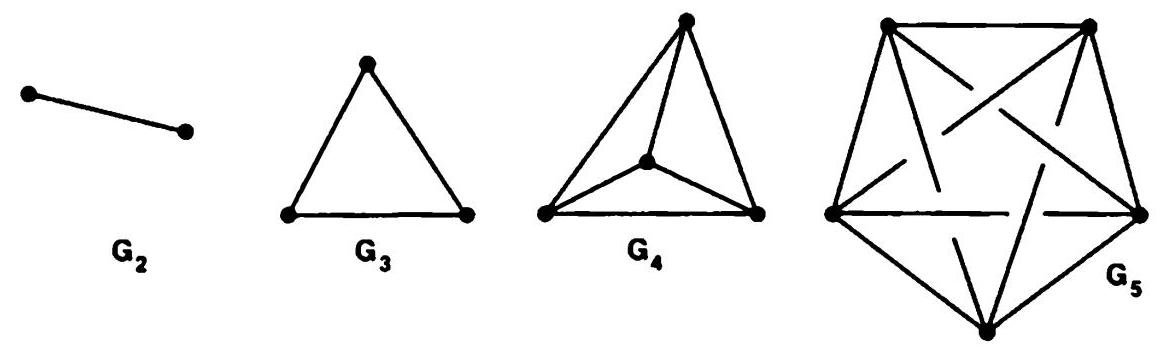
\includegraphics[width=1.0\textwidth]{images/64.1.jpg}
\end{center}
\hspace*{3em}

Figure 64.1
\end{example}
\end{centeredblock}

\begin{centeredblock}
\begin{example}
	Another interesting graph arises in considering the classical puzzle: ``Given three houses, \({h}_{1},{h}_{2}\) , and \({h}_{3}\) , and three utilities, \(g\) (for gas), \(w\) (for water), and \(e\) (for electricity), can you connect each utility to each house without letting any of the connecting lines cross?'' Formulated mathematically, this is just the question whether the graph pictured in Figure 64.2, which is called the utilities graph. can be imbedded in \({\mathbb{R}}^{2}\) . Again, a little experimentation will convince you that it cannot, a fact that we shall prove shortly
\end{example}
\end{centeredblock}

\begin{definition}
	A theta space \(X\) is a Hausdorff space that is written as the union of three arcs \(A,B\) , and \(C\) , each pair of which intersect precisely in their end points. (The space \(X\) is of course homeomorphic to the Greek letter theta.)
\end{definition}

\begin{center}
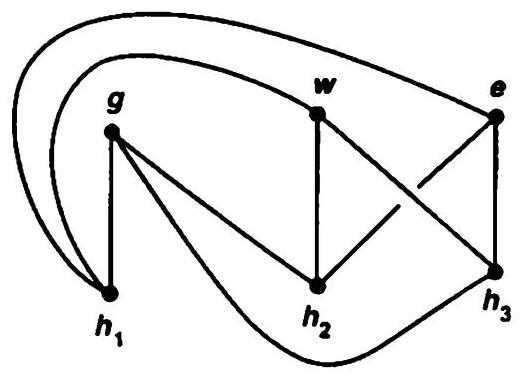
\includegraphics[width=0.4\textwidth]{images/64.2.jpg}
\end{center}
\hspace*{3em} 

Figure 64.2

Note that as it stands, a theta space \(X\) is not a linear graph, for the arcs in question intersect in more than a common end point. One can write it as a graph, however, by breaking each of the arcs \(A,B\) , and \(C\) up into two arcs with an end point in common.

\begin{lemma}
	Let \(X\) be a theta space that is a subspace of \({S}^{2}\) ; let \(A,B\) , and \(C\) be the arcs whose union is \(X\) . Then \(X\) separates \({S}^{2}\) into three components, whose boundaries are \(A \cup  B,B \cup  C\) , and \(A \cup  C\) , respectively. The component having \(A \cup  B\) as its boundary equals one of the components of \({S}^{2} - A \cup  B\) .
\end{lemma}

\begin{proof}
	Let \(a\) and \(b\) be the end points of the arcs \(A,B\) , and \(C\) . Consider the simple closed curve \(A \cup  B\) ; it separates \({S}^{2}\) into two components \(U\) and \({U}^{\prime }\) , each of which is open in \({S}^{2}\) and has boundary \(A \cup  B\) . See Figure 64.3.
\begin{center}
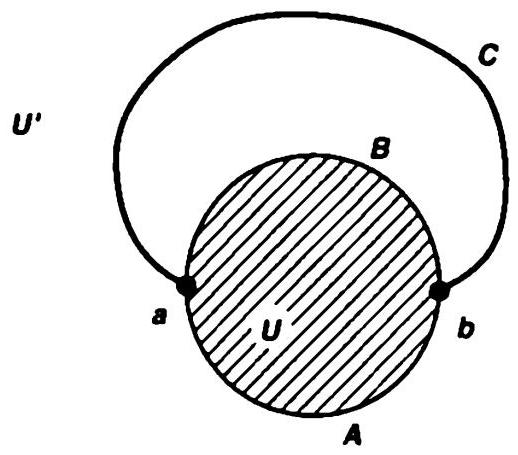
\includegraphics[width=0.4\textwidth]{images/64.3.jpg}
\end{center}
\hspace*{3em} 

Figure 64.3

The space \(C - a - b\) is connected, so it is contained in one of these components, say in \({U}^{\prime }\) . Then consider the two spaces \(\widetilde{U} = U \cup  A \cup  B\) and \(C\) ; each is connected. Neither separates \({S}^{2}\) , for \(C\) is an arc, and the complement of \(\widetilde{U}\) is the connected set \({U}^{\prime }\) . Since the intersection of these two sets consists of the two points \(a\) and \(b\) , their union separates \({S}^{2}\) into two components \(V\) and \(W\) , by Theorem 63.5. It follows that \({S}^{2} -\)  \(( {A \cup  B \cup  C})\) is the union of the three disjoint connected sets \(U,V\) , and \(W\) ; because they are open in \({S}^{2}\) , they are the components of \({S}^{2} - ( {A \cup  B \cup  C})\) . The component \(U\) has \(A \cup  B\) as its boundary. Symmetry implies that the other two have \(B \cup  C\) and

\(A \cup  C\) as their boundaries.
\end{proof}
\begin{theorem}
	Let \(X\) be the utilities graph. Then \(X\) \index{Utilities graph!nonembeddability}cannot be imbedded in the plane.
\end{theorem}

\begin{proof}
	If \(X\) can be imbedded in the plane, then it can be imbedded in \({S}^{2}\) . So suppose \(X\) is a subspace of \({S}^{2}\) . We derive a contradiction.
We use the notation of Example 2, where \(g,w,e,{h}_{1},{h}_{2}\) , and \({h}_{3}\) are the vertices of \(X\) . Let \(A,B\) , and \(C\) be the following arcs contained in \(X\) :

\[
\begin{aligned}  & A = g{h}_{1}w, \\  & B = g{h}_{2}w \\  & C = g{h}_{3}w. \end{aligned}
\]

Each pair of these arcs intersect in their end points \(g\) and \(w\) alone; hence \(Y = A \cup  B \cup  C\) is a \index{Theta space!separates \({S}^{2}\)}\index{Separation theorem: closed topologist's sine curve in \({S}^{2}\)!theta space in \({S}^{2}\)}theta space. The space \(Y\) separates \({S}^{2}\) into three components \(U,V\) , and \(W\) , whose boundaries are \(A \cup  B,B \cup  C\) , and \(A \cup  C\) , respectively. See Figure 64.4.

Now the vertex \(e\) of \(X\) lies in one of these three components, so that the arcs \(e{h}_{1}\) and \(e{h}_{2}\) and \(e{h}_{3}\) of \(X\) lie in the closure of that component. That component cannot be \(U\) , for \(\widetilde{U}\) is contained in \(U \cup  A \cup  B\) , a set that does not contain the point \({h}_{3}\) . Similarly, the component containing \(e\) cannot be \(V\) or \(W\) , because \(\widetilde{V}\) does not contain \({h}_{1}\) , and \(\bar{W}\) does not contain \({h}_{2}\) . Thus, we have reached a contradiction.

\begin{center}
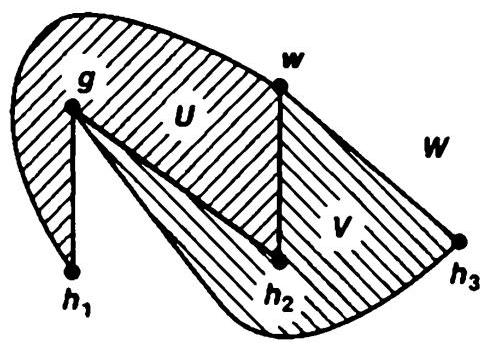
\includegraphics[width=0.4\textwidth]{images/64.4.jpg}
\end{center}
\hspace*{3em} 

Figure 64.4
\end{proof}
\begin{lemma}
	Let \(X\) be a subspace of \({S}^{2}\) that is a \index{complete graph@Complete graph}complete graph on four vertices \({a}_{1}\) , \({a}_{2},{a}_{3}\) , and \({a}_{4}\) . Then \(X\) separates \({S}^{2}\) into four components. The boundaries of these components are the sets \({X}_{1},{X}_{2},{X}_{3}\) , and \({X}_{4}\) , where \({X}_{i}\) is the union of those edges of \(X\) that do not have \({a}_{i}\) as a vertex.
\end{lemma}

\begin{proof}
	Let \(Y\) be the union of all the arcs of \(X\) different from the arc \({a}_{2}{a}_{4}\) . Then we can write \(Y\) as a theta space by setting
\[
\begin{aligned}  & A = {a}_{1}{a}_{2}{a}_{3}, \\  & B = {a}_{1}{a}_{3}, \\  & C = {a}_{1}{a}_{4}{a}_{3}. \end{aligned}
\]

See Figure 64.5. The arcs \(A,B\) , and \(C\) intersect in their end points \({a}_{1}\) and \({a}_{3}\) alone, and their union is \(Y\) .

\begin{center}

\includegraphics[width=0.5\textwidth]{64.5.jpg}
\end{center}
\hspace*{3em} 

Figure 64.5

The space \(Y\) separates \({S}^{2}\) into three components \(U,V\) , and \(W\) , whose boundaries are \(A \cup  B,B \cup  C\) , and \(A \cup  C\) , respectively. The space \({a}_{2}{a}_{4} - {a}_{2} - {a}_{4}\) , being connected, must lie in one of them. It cannot lie in \(U\) , because \(A \cup  B\) does not contain \({a}_{4}\) . And it cannot lie in \(V\) because \(B \cup  C\) does not contain \({a}_{2}\) . Hence it must lie in \(W\) .

Now \(\bar{U} \cup  \bar{V}\) is connected because \(\bar{U}\) and \(\bar{V}\) are connected and have nonempty intersection \(B\) . Furthermore, the set \(\bar{U} \cup  \bar{V}\) does not separate \({S}^{2}\) , because its complement is \(W\) . Similarly, the arc \({a}_{2}{a}_{4}\) is connected and does not separate \({S}^{2}\) . And the sets \({a}_{2}{a}_{4}\) and \(\bar{U} \cup  \bar{V}\) intersect in the points \({a}_{2}\) and \({a}_{4}\) alone. It follows from Theorem 63.5 that \({a}_{2}{a}_{4} \cup  \bar{U} \cup  \bar{V}\) separates \({S}^{2}\) into two components \({W}_{1}\) and \({W}_{2}\) . Then \({S}^{2} - Y\) is the union of the four disjoint connected sets \(U,V,{W}_{1}\) , and \({W}_{2}\) . Since these sets are open, they are the components of \({S}^{2} - Y\) .

Now one of these components, namely \(U\) , has the graph \(A \cup  B = {X}_{4}\) as its boundary. Symmetry implies that the other three have \({X}_{1},{X}_{2}\) , and \({X}_{3}\) as their respective boundaries.
\end{proof}
\begin{theorem}
	The complete graph on five vertices cannot be imbedded in the plane.
\end{theorem}

\begin{proof}
	Suppose that \(G\) is a subspace of \({S}^{2}\) that is a complete graph on the five vertices \({a}_{1},{a}_{2},{a}_{3},{a}_{4}\) , and \({a}_{5}\) . Let \(X\) be the union of those edges of \(G\) that do not have \({a}_{5}\) as a vertex; then \(X\) is a complete graph on four vertices. The space \(X\) separates \({S}^{2}\) into four components, whose respective boundaries are the graphs \({X}_{1},\ldots ,{X}_{4}\) , where \({X}_{i}\) consists of those edges of \(X\) that do not have \({a}_{i}\) as a vertex. Now the point \({a}_{5}\) must lie in one of these four components. It follows that the connected space
\[
{a}_{1}{a}_{5} \cup  {a}_{2}{a}_{5} \cup  {a}_{3}{a}_{5} \cup  {a}_{4}{a}_{5},
\]

which is the union of those edges of \(G\) that have \({a}_{5}\) as a vertex, must lie in the closure of this component. Then all the vertices \({a}_{1},\ldots ,{a}_{4}\) lie in the boundary of this component. But this is impossible, for none of the graphs \({X}_{i}\) contains all four vertices \({a}_{1},\ldots ,{a}_{4}\) . Thus we reach a contradiction.

It follows from these theorems that if a graph \(G\) contains a subgraph that is a utilities graph or a complete graph on five vertices, then \(G\) cannot be imbedded in the plane. It is a remarkable theorem, due to Kuratowski, that the converse is also true! The proof is not easy.
\end{proof}
\section*{Exercise}

1. Let \(X\) be a space that is written as the union of finitely many arcs \({A}_{1},\ldots ,{A}_{n}\) , each pair of which intersect in at most a common end point.

(a) Show that \(X\) is Hausdorff if and only if each arc \({A}_{i}\) is closed in \(X\) .

(b) Give an example to show that \(X\) need not be Hausdorff. [Hint: See Exercise 5 of  \S 36.]

\section*{§ 65 The Winding Number of a Simple Closed Curve}

If \(h : {S}^{1} \rightarrow  {\mathbb{R}}^{2} - 0\) is a continuous map, then the induced homomorphism \({h}_{ * }\) carries a generator of the fundamental group of \({S}^{1}\) to some integral power of a generator of the fundamental group of \({\mathbb{R}}^{2} - \mathbf{0}\) . This integral power \(n\) is called the \index{Simple closed curve!winding number}winding number of \(h\) with respect to 0. It measures how many times \(h\) ``wraps \({S}^{1}\) around the origin;'' its sign depends of course on the choice of generators. See Figure 65.1. We will introduce it more formally in the next section.

\begin{center}
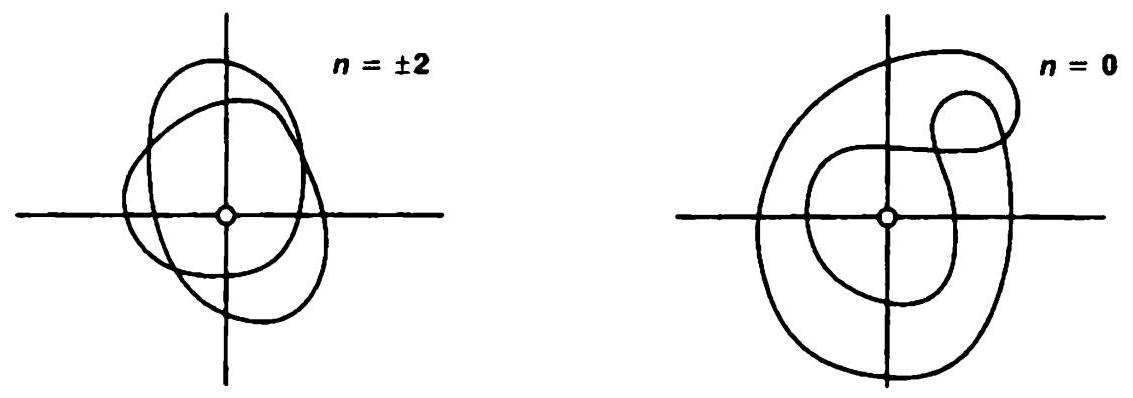
\includegraphics[width=1.0\textwidth]{images/65.1.jpg}
\end{center}
\hspace*{3em} 

Figure 65.1

For the present, we merely ask the question: What can one say about the winding number of \(h\) if \(h\) is injective, that is, if \(h\) is a homeomorphism of \({S}^{1}\) with a simple closed curve \(C\) in \({\mathbb{R}}^{2} - 0\) ? The illustrations in Figure 65.2 suggest the obvious conjecture: If 0 belongs to the unbounded component of \({\mathbb{R}}^{2} - C\) , then \(n = 0\) , while if 0 belongs to the bounded component, then \(n =  \pm  1\) .

\begin{center}
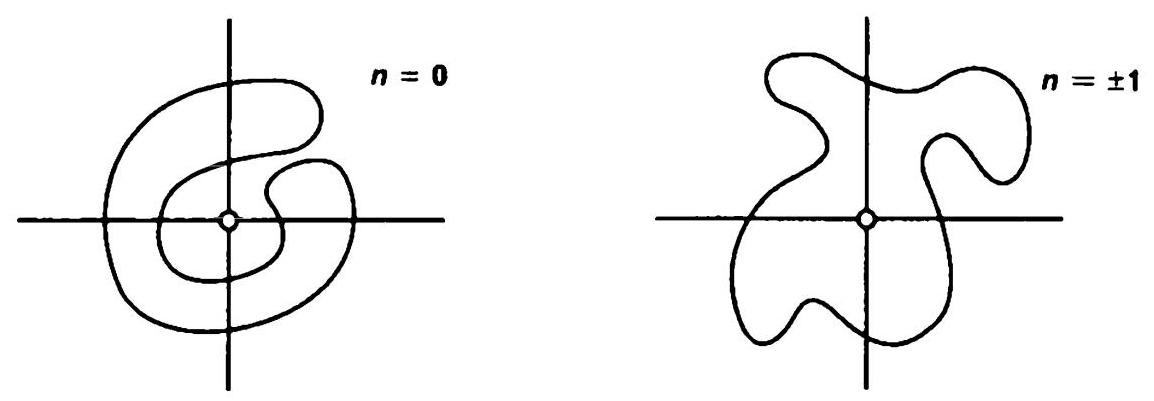
\includegraphics[width=1.0\textwidth]{images/65.2.jpg}
\end{center}
\hspace*{3em} 

Figure 65.2

The first conjecture is easy to prove, for Lemma 61.2 tells us that \(h\) is nulhomotopic if 0 belongs to the unbounded component of \({\mathbb{R}}^{2} - C\) . On the other hand, the second conjecture is surprisingly difficult; it is in fact a rather deep result. We prove it in this section.

As usual, we shall replace \({\mathbb{R}}^{2} \cup  \{ \infty \}\) by \({S}^{2}\) , letting \(p\) be the point corresponding to 0 and \(q\) be the point corresponding to \(\infty\) . Then our conjecture can be reformulated as follows: If \(C\) is a simple closed curve in \({S}^{2}\) , and if \(p\) and \(q\) belong to different components of \({S}^{2} - C\) , then the inclusion mapping \(j : C \rightarrow  {S}^{2} - p - q\) induces an isomorphism of fundamental groups. This is what we shall prove.

First, we prove our result in the case where the simple closed curve \(C\) is contained in a complete graph on four vertices. Then we prove the general case.

\begin{lemma}
	Let \(G\) be a subspace of \({S}^{2}\) that is a complete graph on four vertices \({a}_{1},\ldots ,{a}_{4}\) . Let \(C\) be the subgraph \({a}_{1}{a}_{2}{a}_{3}{a}_{4}{a}_{1}\) , which is a simple closed curve. Let \(p\) and \(q\) be interior points of the edges \({a}_{1}{a}_{3}\) and \({a}_{2}{a}_{4}\) , respectively. Then:

(a) The points \(p\) and \(q\) lie in different components of \({S}^{2} - C\) .

(b) The inclusion \(j : C \rightarrow  {S}^{2} - p - q\) induces an isomorphism of fundamental groups.
\end{lemma}

\begin{proof}
	(a) As in the proof of Lemma 64.3, the theta space \(C \cup  {a}_{1}{a}_{3}\) separates \({S}^{2}\) into three components \(U,V\) , and \(W\) . One of these, say \(W\) , has \(C\) as its boundary; it is the only component whose boundary contains both \({a}_{2}\) and \({a}_{4}\) . Therefore, \({a}_{2}{a}_{4} - {a}_{2} - {a}_{4}\) must lie in \(W\) , so that in partucular, \(q\) belongs to \(W\) . Of course, \(p\) is not in \(W\) because \(p\) belongs to the theta space \(C \cup  {a}_{1}{a}_{3}\) . Now Lemma 64.1 tells us that \(W\) is one of the components of \({S}^{2} - C\) ; therefore, \(p\) and \(q\) belong to different components of \({S}^{2} - C\) .
(b) Let \(X = {S}^{2} - p - q\) . The idea of the proof is the following: We choose a point \(x\) interior to the arc \({a}_{1}{a}_{2}\) , and a point \(y\) interior to the arc \({a}_{3}{a}_{4}\) . And we let \(\alpha\) and \(\beta\) be the broken-line paths

\[
\alpha  = x{a}_{1}{a}_{4}y\;\text{ and }\;\beta  = y{a}_{3}{a}_{2}x.
\]

Then \(\alpha  * \beta\) is a loop lying in the simple closed curve \(C\) . We shall prove that \(\alpha  * \beta\) represents a generator of the fundamental group of \(X\) . It follows that the homomorphism \({j}_{ * } : {\pi }_{1}( {C,x})  \rightarrow  {\pi }_{1}( {X,x})\) is surjective, so that \({j}_{ * }\) must be an isomorphism (since the groups involved are infinite cyclic). See Figure 65.3.

\begin{center}
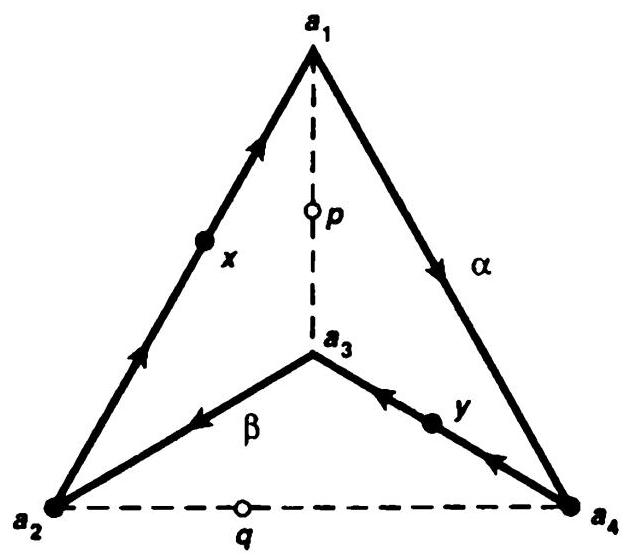
\includegraphics[width=0.5\textwidth]{images/65.3.jpg}
\end{center}
\hspace*{3em} 

Figure 65.3

Let \({D}_{1}\) and \({D}_{2}\) be the arcs

\[
{D}_{1} = p{a}_{3}{a}_{2}q\;\text{ and }\;{D}_{2} = q{a}_{4}{a}_{1}p,
\]

and let \(U = {S}^{2} - {D}_{1}\) and \(V = {S}^{2} - {D}_{2}\) . See Figure 65.4. Then \(X = U \cup  V\) , and \(U \cap  V\) equals \({S}^{2} - D\) , where \(D\) is the simple closed curve \(D = {D}_{1} \cup  {D}_{2}\) . Hence, \(U \cap  V\) has two components, by the Jordan curve theorem. Furthermore, since \(D\) equals the simple closed curve \({a}_{1}{a}_{3}{a}_{2}{a}_{4}{a}_{1}\) , the result of (a) implies that the points \(x\) and \(y\) , which lie interior to the other two edges of the graph \(G\) , lie in different components of \({S}^{2} - D\)

\begin{center}
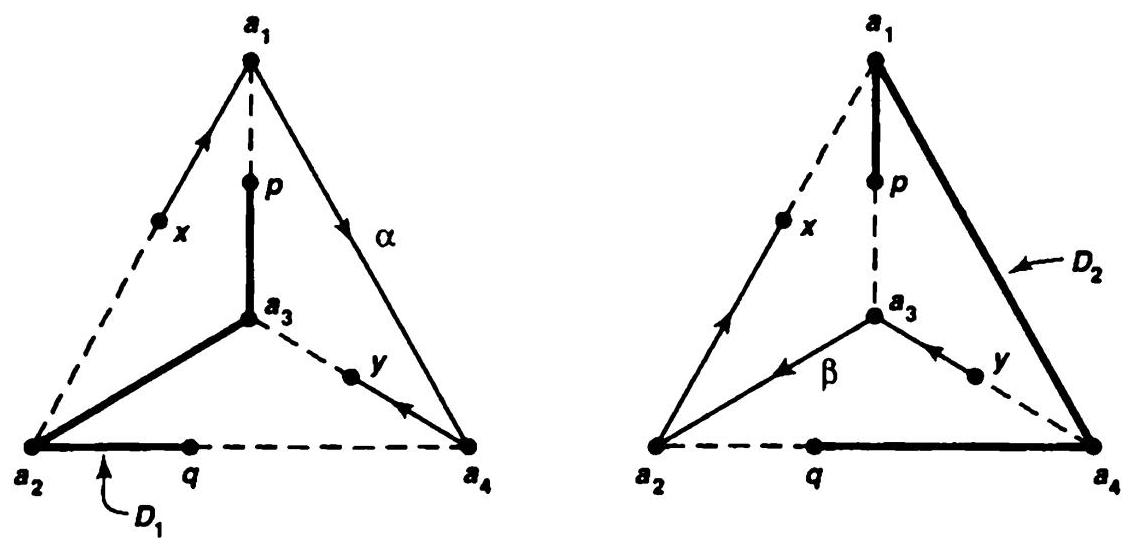
\includegraphics[width=1.0\textwidth]{images/65.4.jpg}
\end{center}
\hspace*{3em} 

Figure 65.4

The hypotheses of Theorem 63.1 are thus satisfied. The path \(\alpha\) is a path in \(U\) from \(x\) to \(y\) , while \(\beta\) is a path in \(V\) from \(y\) to \(x\) . Because the fundamental group of \(X\) is infinite cyclic, the loop \(\alpha  * \beta\) represents a generator of this group.

Now we prove our main theorem.
\end{proof}
\begin{theorem}
	Let \(C\) be a simple closed curve in \({S}^{2}\) ; let \(p\) and \(q\) lie in different components of \({S}^{2} - C\) . Then the inclusion mapping \(j : C \rightarrow  {S}^{2} - p - q\) induces an isomorphism of fundamental groups.
\end{theorem}

\begin{proof}
	The proof involves constructing a complete graph on four vertices that contains \(C\) as a subgraph.
Step 1. Let \(a,b\) , and \(c\) be three distinct points of \({\mathbb{R}}^{2}\) . If \(A\) is an arc with end points points \(a\) and \(b\) , and if \(B\) is an arc with end points \(b\) and \(c\) , then there exists an arc contained in \(A \cup  B\) with end points \(a\) and \(c\) .

Choose paths \(f : I \rightarrow  A\) from \(a\) to \(b\) , and \(g : I \rightarrow  B\) from \(b\) to \(c\) , such that \(f\) and \(g\) are homeomorphisms. Let \({t}_{0}\) be a smallest point of \(I\) such that \(f( {t}_{0})  \in  B\) ; and let \({t}_{1}\) be the point of \(I\) such that \(g( {t}_{1})  = f( {t}_{0})\) . Then the set \(f( [  {0,{t}_{0}}]  )  \cup  g( [  {{t}_{1},1}]  )\) is the required arc. (If \({t}_{0} = 0\) or \({t}_{1} = 1\) , one of these sets consists of a single point.) See Figure 65.5.

\begin{center}
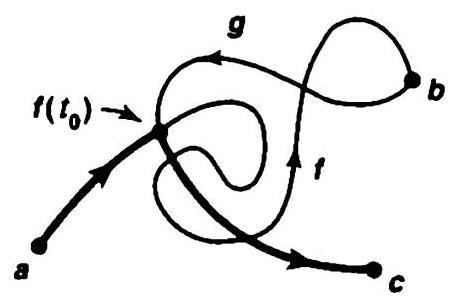
\includegraphics[width=0.4\textwidth]{images/65.5.jpg}
\end{center}
\hspace*{3em} 

Figure 65.5

Step 2. We show that if \(U\) is an open set of \({\mathbb{R}}^{2}\) , any two points of \(U\) that can be connected by a path in \(U\) are the end points of an arc lying in \(U\) .

If \(x,y \in  U\) , set \(x \sim  y\) if \(x = y\) or if there is an arc in \(U\) with end points \(x\) and \(y\) . The result of Step 1 shows that this is an equivalence relation. The equivalence classes are open, for if the \(\epsilon\) -neighborhood of \(x\) lies in \(U\) , it consists of points equivalent to \(x\) . Since \(U\) is connected, there is only one such equivalence class.

Step 3. Let \(C\) be a simple closed curve in \({\mathbb{R}}^{2}\) . We construct a subspace \(G\) of \({\mathbb{R}}^{2}\) that is a complete graph on four vertices \({a}_{1},\ldots ,{a}_{4}\) such that \(C\) equals the subgraph \({a}_{1}{a}_{2}{a}_{3}{a}_{4}{a}_{1}\) .

For convenience, we assume that 0 lies in the bounded component of \({\mathbb{R}}^{2} - C\) . Consider the \(x\) -axis \(\mathbb{R} \times  0\) in \({\mathbb{R}}^{2}\) ; let \({a}_{1}\) be the largest point on the negative \(x\) -axis that lies in \(C\) , and let \({a}_{3}\) be the smallest point on the positive \(x\) -axis that lies in \(C\) . Then the line segment \({a}_{1}{a}_{3}\) lies in the closure of the bounded component of \({\mathbb{R}}^{2} - C\) .

Let us write \(C\) as the union of two arcs \({C}_{1}\) and \({C}_{2}\) with end points \({a}_{1}\) and \({a}_{3}\) . Let \(a\) be a point of the unbounded component of \({\mathbb{R}}^{2} - C\) . Since \({C}_{1}\) and \({C}_{2}\) do not separate \({\mathbb{R}}^{2}\) , we can choose paths \(\alpha  : I \rightarrow  {\mathbb{R}}^{2} - {C}_{1}\) and \(\beta  : I \rightarrow  {\mathbb{R}}^{2} - {C}_{2}\) from \(a\) to 0; in view of Step 2, we may assume that \(\alpha\) and \(\beta\) are injective. Let \({a}_{2} = \alpha ( {t}_{0})\) , where \({t}_{0}\) is the smallest number such that \(\alpha ( {t}_{0})  \in  C\) ; then \({a}_{2}\) is a point interior to \({C}_{2}\) . Similarly, let \({a}_{4} = \beta ( {t}_{1})\) , where \({t}_{1}\) is the smallest number such that \(\beta ( {t}_{1})  \in  C\) ; then \({a}_{4}\) is an interior point of \({C}_{1}\) . Then \(\alpha ( [  {0,{t}_{0}}]  )\) and \(\beta ( [  {0,{t}_{1}}]  )\) are arcs joining \(a\) to \({a}_{2}\) and \({a}_{4}\) , respectively; by Step 2, their union contains an arc with end points \({a}_{2}\) and \({a}_{4}\) ; thus arc intersects \(C\) only in these two points. This arc, along with the line segment \({a}_{1}{a}_{3}\) and the curve \(C\) , forms the desired graph. See Figure 65.6.

\begin{center}
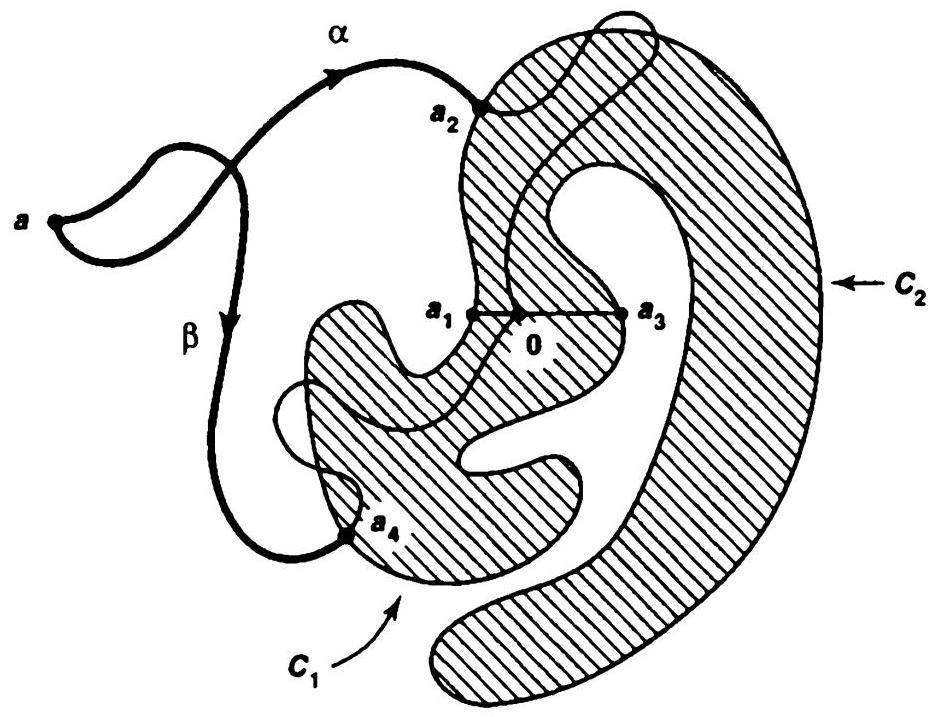
\includegraphics[width=0.8\textwidth]{images/65.6.jpg}
\end{center}
\hspace*{3em} 

Figure 65.6

Step 4. It follows from the result of Step 3 and the preceding lemma that for some pair of points \(p,q\) lying in different components of \({S}^{2} - C\) , the inclusion \(j : C \rightarrow\)  \({S}^{2} - p - q\) induces an isomorphism of fundamental groups. To complete the proof, we need only show that the same holds for any pair \(p,q\) of points lying in different components of \({S}^{2} - C\) . For that purpose, it suffices to prove the following:

Let \(D\) be a simple closed curve in \({\mathbb{R}}^{2}\) ; suppose 0 lies in the bounded component of \({\mathbb{R}}^{2} - D\) . Let \(p\) be another point of this component. If inclusion \(j : D \rightarrow  {\mathbb{R}}^{2} - 0\) induces an isomorphism of fundamental groups, then so does the inclusion \(k : D \rightarrow  {\mathbb{R}}^{2} - p\) .

Let \(f.{\mathbb{R}}^{2} - p \rightarrow  {\mathbb{R}}^{2} - 0\) be the homeomorphism \(f( x)  = x - p\) . It suffices to show that the map

\[
D\overset{k}{ \rightarrow  }{\mathbb{R}}^{2} - p\overset{f}{ \rightarrow  }{\mathbb{R}}^{2} - 0
\]

indices an isomorphism of fundamental groups. Let \(\alpha\) be a path in \({\mathbb{R}}^{2} - D\) from 0 to \(p\) , and let \(F : D \times  I \rightarrow  {\mathbb{R}}^{2} - 0\) be the map \(F( {x,t})  = x - \alpha ( t)\) . Then \(F\) is a homotopy between \(j\) and \(f \circ  k\) ; since \(j\) induces an isomorphism, so does \(f \circ  k\) . (See Corollary 58.5).

This theorem is a special case of a rather deep theorem of algebraic topology, concerning the ``linking number'' of two disjoint subspaces of \({S}^{m + n + 1}\) , one homeomorphic to an \(m\) -sphere and the other homeomorphic to an \(n\) -sphere; it is related to the Alexander duality theorem. (See 		\cite{Munkres1993}, p. 433.) The special case of our theorem is that of a 0-sphere (i.e., a two-point space) and a 1-sphere (i.e., a simple closed curve) in \({S}^{2}\) .
\end{proof}
\section*{§ 66 The Cauchy Integral Formula}

One of the central theorems in the study of functions of a complex variable is the one concerning the Cauchy integral formula for analytic functions. For the classical version of this theorem, one needs to assume not only the Jordan curve theorem, but also the winding-number theorem of the last section. There is, however, a reformulation of the Cauchy integral theorem that avoids using these results; this version of the theorem, although it is rather less natural, is the one now commonly found in texts on the subject.

Since we have the Jordan curve theorem at our disposal, we shall set ourselves the task of deriving the Cauchy integral formula in its classical version from the reformulated version.

We begin by introducing the notion of ``winding number'' more formally.

\begin{definition}
	Let \(f\) be a loop in \({\mathbb{R}}^{2}\) , and let \(a\) be a point not in the image of \(f\) . Set

\[
g( s)  = [  {f( s)  - a}]  /\parallel f( s)  - a\parallel
\]

then \(g\) is a loop in \({S}^{1}\) . Let \(p : \mathbb{R} \rightarrow  {S}^{1}\) be the standard covering map, and let \(\widetilde{g}\) be a lifting of \(g\) to \({S}^{1}\) . Because \(g\) is a loop, the difference \(\widetilde{g}( 1)  - \widetilde{g}( 0)\) is an integer. This integer is called the winding number of \(f\) with respect to \(a\) , and is denoted \(\index{n@\(n( {f,a})\)} n( {f,a})\) .
\end{definition}

Note that \(n( {f,a})\) is independent of the choice of the lifting of \(g\) . For if \(\widetilde{g}\) is one lifting of \(g\) , then uniqueness of liftings implies that any other lifting of \(g\) has the form \(\widetilde{g}( s)  + m\) for some integer \(m\) .

\begin{definition}
	Let \(F : I \times  I \rightarrow  X\) be a continuous map such that \(F( {0,t})  = F( {1,t})\) for all \(t\) . Then for each \(t\) , the map \({f}_{t}( s)  = F( {s,t})\) is a loop in \(X\) . The map \(F\) is called a free homotopy between the loops \({f}_{0}\) and \({f}_{1}\) . It is a homotopy of loops in which the base point of the loop is allowed to move during the homotopy.
\end{definition}

\begin{lemma}
	Let \(f\) be a loop in \({\mathbb{R}}^{2} - a\) .

(a) If \(\bar{f}\) is the reverse of \(f\) , then \(n( {\bar{f},a})  =  - n( {f,a})\) .

(b) If \(f\) is freely homotopic to \({f}^{\prime }\) , through loops lying in \({\mathbb{R}}^{2} - a\) , then \(n( {f,a})  =\)  \(n( {{f}^{\prime },a})\) .

(c) If \(a\) and \(b\) lie in the same component of \({\mathbb{R}}^{2} - f( I)\) , then \(n( {f,a})  = n( {f,b})\) .
\end{lemma}

\begin{proof}
	(a) To compute \(n( {\bar{f},a})\) , one replace \(s\) by \(1 - s\) throughout the definition. This has the effect of changing \(\widetilde{g}( 1)  - \widetilde{g}( 0)\) by a sign
(b) Let \(F\) be a free homotopy between \(f\) and \({f}^{\prime }\) . Define \(G : 1 \times  I \rightarrow  {S}^{1}\) by the equation

\[
G( {s,t})  = [  {F( {s,t})  - a}]  /\parallel F( {s,t})  - a\parallel .
\]

Let \(\bar{G}\) be a lifting of \(G\) to \(\mathbb{R}\) . Then \(\widetilde{G}( {1,t})  - \widetilde{G}( {0,t})\) is an integer for each \(t\) ; being continuous, it is constant.

(c) Let \(\alpha\) be a path in \({\mathbb{R}}^{2} - f( l)\) from \(a\) to \(b\) . Note that by definition, \(n( {f,a})  =\)  \(n( {f - a,0})\) . Since \(f( s)  - \alpha ( t)\) is a free homotopy in \({\mathbb{R}}^{2} - 0\) between \(f - a\) and \(f - b\) , our result follows.
\end{proof}
\begin{definition}
	Let \(f\) be a loop in \(X\) . We call \(f\) a \index{Simple loop} provided \(f( s)  = f( {s}^{\prime })\) only if \(s = {s}^{\prime }\) or if one of the points \(s,{s}^{\prime }\) is 0 and the other is 1 . If \(f\) is a \index{simple loop@Simple loop}simple loop, its image set is a simple closed curve in \(X\) .
\end{definition}

\begin{theorem}
	Let \(f\) be a simple loop in \({\mathbb{R}}^{2}\) . If a lies in the unbounded component of \({\mathbb{R}}^{2} - f( 1)\) , then \(n( {f,a})  = 0\) ; while if a lies in the bounded component, \(n( {f,a})  =  \pm  1\) .
\end{theorem}

\begin{proof}
	Since \(n( {f,a})  = n( {f - a,0})\) , we may restrict ourselves to the case \(a = 0\) . Furthermore, we may assume that the base point of \(f\) lies on the positive \(x\) -axis. For one can gradually rotate \({\mathbb{R}}^{2} - 0\) until the base point of \(f\) is such a point; this modifies \(f\) by a free homotopy, so it does not affect the conclusion of the theorem.
So let \(f\) be a simple loop in \(X = {\mathbb{R}}^{2} - 0\) based at a point \({x}_{0}\) of the positive \(x\) - axis. Let \(C\) be the simple closed curve \(f( I)\) . We show that if0lies in the bounded component of \({\mathbb{R}}^{2} - C\) , then \([  f]\) \index{Simple closed curve!generates \({\pi }_{1}\) of \({\mathbb{R}}^{2} - 0\)}generates \({\pi }_{1}( {X,{x}_{0}})\) , while if 0 lies in the unbounded component, \([  f]\) is trivial.

The map \(f\) induces, \({via}\) the standard quotient map \(p : I \rightarrow  {S}^{1}\) , a homeomorphism \(h : {S}^{1} \rightarrow  C\) . The element \([  p]\) generates the fundamental group of \({S}^{1}\) , so \({h}_{ * }[  p]\) generates the fundamental group of \(C\) . If0lies in the bounded component of \({\mathbb{R}}^{2} - C\) , Theorem 65.2 tells us that \({j}_{ * }{h}_{ * }[  p] = [  f]\) generates the fundamental group of \({\mathbb{R}}^{2} - \mathbf{0}\) , where \(j : C \rightarrow  {\mathbb{R}}^{2} - 0\) is the inclusion. On the other hand, if0lies in the unbounded component of \({\mathbb{R}}^{2} - C\) , then \(j \circ  h\) is nulhomotopic by Lemma 61.2, so that \([  f]\) is trivial.

Now we show that if \([  f]\) generates \({\pi }_{1}( {X,{x}_{0}})\) , then \(n( {f,\mathbf{0}})  =  \pm  1\) , while if \([  f]\) is trivial, \(n( {f,\mathbf{0}})  = 0\) . Since the retraction \(x \rightarrow  x/\parallel x\parallel\) of \({\mathbb{R}}^{2} - \mathbf{0}\) onto \({S}^{1}\) induces an isomorphism of fundamental groups, the loop \(g( s)  = f( s) /\parallel f( s) \parallel\) represents a generator of \({\pi }_{1}( {{S}^{1},{b}_{0}})\) in the first case, and the identity element in the second case. If we examine the isomorphism \(\phi  : {\pi }_{1}( {{S}^{1},{b}_{0}})  \rightarrow  \mathbb{Z}\) constructed in the proof of Theorem 54.5, we see this means that when we lift \(g\) to a path \(\bar{g}\) in \(\mathbb{R}\) beginning at 0, the path \(\widetilde{g}\) ends at \(\pm  1\) in the first case, and at 0 in the second.
\end{proof}
\begin{definition}
	Let \(f\) be a simple loop in \({\mathbb{R}}^{2}\) . We say \(f\) is a \index{Counterclockwise loop} if \(n( {f,a})  =  + 1\) for some \(a\) (and hence for every \(a\) ) in the bounded component of \({\mathbb{R}}^{2} - f( I)\) . We say it is a clockwise loop if \(n( {f,a})  =  - 1\) . The standard loop \(p( s)  =\)  \(( {\cos {2\pi s},\sin {2\pi s}})\) is thus a \index{counterclockwise loop@Counterclockwise loop}counterclockwise loop.
\end{definition}

\section*{Application to complex variables}

We now relate \index{Winding number!as an integral}winding numbers to complex line integrals.

\begin{lemma}
	Let \(f\) be a piecewise-differentiable loop in the complex plane; let a be a point not in the image of \(f\) . Then

\[
n( {f,a})  = \frac{1}{2\pi i}{\int }_{f}\frac{dz}{z - a}.
\]

This equation is often used as the definition of the winding number of \(f\) .
\end{lemma}

\begin{proof}
	The proof is a simple exercise in computation. Let \(p : \mathbb{R} \rightarrow  {S}^{1}\) be the standard covering map. Let \(r( s)  = \parallel f( s)  - a\parallel\) and \(g( s)  = [  {f( s)  - a}]  /r( s)\) . Let \(\widetilde{g}\) be a lifting of \(g\) to \(\mathbb{R}\) . Set \(\theta ( s)  = {2\pi }\widetilde{g}( s)\) . Then \(f( s)  - a = r( s) \exp ( {{i\theta }( s) })\) , so that
\[
{\int }_{f}\frac{dz}{z - a} = {\int }_{0}^{1}[  {( {{r}^{\prime }{e}^{i\theta } + {ir}{\theta }^{\prime }{e}^{i\theta }}) /r{e}^{i\theta }}]  {ds}
\]

\[
= {[  \log r( s)  + i\theta ( s) ]  }_{0}^{1}
\]

\[
= i[  {\theta ( 1)  - \theta ( 0) }]
\]

\[
= {2\pi i}[  {\widetilde{g}( 1)  - \widetilde{g}( 0) }]  .
\]
\end{proof}
\begin{theorem}[Cauchy integral formula-classical version]
	Let \(C\) be a simple closed piecewise-differentiable curve in the complex plane. Let \(B\) be the bounded component of \({\mathbb{R}}^{2} - C\) . If \(F( z)\) is analytic in an open set \(\Omega\) that contains \(B\) and \(C\) , then for each point \(a\) of \(B\) ,

\[
F( a)  =  \pm  \frac{1}{2\pi i}{\int }_{C}\frac{F( z) }{z - a}{dz}.
\]

The sign is + if \(C\) is oriented counterclockwise, and - otherwise.
\end{theorem}

\begin{proof}
	We derive this formula from the version of it proved in Ahlfors 		\cite{Ahlfors1979}, which is the following:
Let \(F\) be analytic in a region \(\Omega\) . Let \(f\) be a piecewise-differentiable loop in \(\Omega\) . Assume that \(n( {f,b})  = 0\) for each \(b\) not in \(\Omega\) . If \(a \in  \Omega\) and \(a\) is not in the image of \(f\) , then

\[
n( {f,a})  \cdot  F( a)  = \frac{1}{2\pi i}{\int }_{f}\frac{F( z) }{z - a}{dz}.
\]

We apply this result to a piecewise-differentiable parametrization \(f\) of our simple closed curve \(C\) . The condition \(n( {f,b})  = 0\) holds for each \(b\) not in \(\Omega\) , since any such \(b\) lies in the unbounded component of \({\mathbb{R}}^{2} - C\) . Furthermore, \(n( {f,a})  =  \pm  1\) whenever \(a\) is in \(B\) , the sign depending on the orientation of \(C\) , by Theorem 66.2. The theorem follows.

Note that one cannot even state the classical version of the Cauchy integral theorem without knowing the Jordan curve theorem. To prove it requires even more, namely, knowledge of the winding number of a simple closed curve. It is of interest to note that this latter result can be proved (at least in the differentiable case) by an entirely different method, using the general version of Green's Theorem, proved in analysis. This proof is outlined in Exercise 2.
\end{proof}
\section*{Exercises}
\begin{enumerate}[itemsep=0.4em, parsep=0pt, topsep=0pt, partopsep=0pt, leftmargin=*, label=\arabic*., ref=\arabic*]
\item Let \(f\) be a loop in \({\mathbb{R}}^{2} - a\) ; let \(g( s)  = [  {f( s)  - a}]  /\parallel f( s)  - a\parallel\) The map \(g\) induces, via the standard quotient map \(p : I \rightarrow  {S}^{1}\) , a continuous map \(h : {S}^{1} \rightarrow  {S}^{1}\) . Show that \(n( {f,a})\) equals the degree of \(h\) , as defined in Exercise 9 of \( \S {58}\) .
\item This exercise assumes some familiarity with analysis on manifolds. \textsl{Theorem.} Let \(C\) be a simple closed curve in \({\mathbb{R}}^{2}\) that is a smooth submanifold of \({\mathbb{R}}^{2}\) ; let \(f : I \rightarrow  C\) be a simple loop smoothly parameterizing \(C\) . If 0 is a point of the bounded component of \({\mathbb{R}}^{2} - C\) , then \(n( {f,\mathbf{0}})  =  \pm  1\) .  \textsl{Proof.} Let \(U\) be the bounded component of \({\mathbb{R}}^{2} - C\) . Let \(B\) be a closed \(\epsilon\) -ball centered at 0 that lies in \(U\) ; let \(S = \operatorname{Bd}B\) . Let \(M\) equal the closure of \(U - B\) .
  \begin{enumerate}[itemsep=0.2em, parsep=0pt, topsep=0pt, partopsep=0pt, leftmargin=*, label=(\alph*), align=left]
  \item Show \(M\) is a smooth \index{2-manifold with boundary}2-manifold with boundary \(C \cup  S\) .
  \item Apply Green's theorem to show that \({\int }_{C}{dz}/z =  \pm  {\int }_{S}{dz}/z\) , the sign depending on the orientations of \(S\) and \(C\) . [Hint: Set \(P =  - y/( {{x}^{2} + {y}^{2}})\) and \(. {Q = x/( {{x}^{2} + {y}^{2}}) .}]\)
  \item Show that the second integral equals \(\pm  {2\pi i}\).
  \end{enumerate}
\end{enumerate}
\chapteropening{The Seifert-van Kampen Theorem}

\booksection{67}{Direct Sums of Abelian Groups}

 In this section, we shall consider only groups that are abelian. As is usual, we shall write such groups additively. Then 0 denotes the identity element of the group, \(- x\) denotes the inverse of \(x\), and \({nx}\) denotes the \(n\) -fold sum \(x + \cdots + x\).

Suppose \(G\) is an abelian group, and \({\{ G_{\alpha }\} }_{\alpha \in J}\) is an indexed family of subgroups of \(G\). We say that the groups \(G_{\alpha }\) generate \(G\) if every element \(x\) of \(G\) can be written as a finite sum of elements of the groups \(G_{\alpha }\). Since \(G\) is abelian, we can always rearrange such a sum to group together terms that belong to a single \(G_{\alpha }\) ; hence we can always write \(x\) in the form

\[
x = x_{{\alpha }_{1}} + \cdots + x_{{\alpha }_{n}},
\]
where the indices \({\alpha }_{i}\) are distinct. In this case, we often write \(x\) as the formal sum \(x = \mathop{\sum }\limits_{{\alpha \in J}}x_{\alpha }\), where it is understood that \(x_{\alpha } = 0\) if \(\alpha\) is not one of the indices \({\alpha }_{1}\), \(\ldots ,{\alpha }_{n}\).

If the groups \(G_{\alpha }\) generate \(G\), we often say that \(G\) is the sum of the groups \(G_{\alpha }\), writing \(G = \mathop{\sum }\limits_{{\alpha \in J}}G_{\alpha }\) in general, or \(G = G_{1} + \cdots + G_{n}\) in the case of the finite index set \(\{ 1,\ldots, n\}\).

Now suppose that the groups \(G_{\alpha }\) generate \(G\), and that for each \(x \in G\), the expression \(x = \sum {x}_{\alpha }\) for \(x\) is unique. That is, suppose that for each \(x \in G\), there is only one \(J\) -tuple \({( x_{\alpha }) }_{\alpha \in J}\) with \(x_{\alpha } = 0\) for all but finitely many \(\alpha\) such that \(x = \sum {x}_{\alpha }\). Then \(G\) is said to be the direct sum of the groups \(G_{\alpha }\), and we write

\[
G = {\bigoplus }_{\alpha \in J}G_{\alpha }
\]
or in the finite case, \(G = G_{1} \oplus \cdots \oplus {G}_{n}\)

\begin{centeredblock}
\begin{example}
\label{ex:\thesection.\theexample}
The cartesian product \(\mathbb{R}^{\omega }\) is an abelian group under the operation of coordinate-wise addition. The set \(G_{n}\) consisting of those tuples \(( x_{i})\) such that \(x_{i} = 0\) for \(i \neq n\) is a subgroup isomorphic to \(\mathbb{R}\). The groups \(G_{n}\) generate the subgroup \(\mathbb{R}^{\infty }\) of \(\mathbb{R}^{\omega }\), indeed, \(\mathbb{R}^{\infty }\) is their direct sum.
\end{example}
\end{centeredblock}

A useful characterization of direct sums is given in the following lemma, we call it the extension condition for direct sums.

\begin{lemma}
\label{lem:\thetheorem}
Let \(G\) be an abelian group; let \(\{ G_{\alpha }\}\) be a family of subgroups of \(G\). If \(G\) is the direct sum of the groups \(G_{\alpha }\), then \(G\) satisfies the following condition:

Given any abelian group \(H\) and any family of homomorphisms \((*)\) \(h_{\alpha } : G_{\alpha } \rightarrow H\), there exists a homomorphism \(h : G \rightarrow H\) whose restriction to \(G_{\alpha }\) equals \(h_{\alpha }\), for each \(\alpha\).

Furthermore, \(h\) is unique. Conversely, if the groups \(G_{\alpha }\) generate \(G\) and the extension condition (*) holds, then \(G\) is the direct sum of the groups \(G_{\alpha }\).
\end{lemma}

\begin{proof}
We show first that if \(G\) has the stated extension property, then \(G\) is the direct sum of the \(G_{\alpha }\). Suppose \(x = \sum {x}_{\alpha } = \sum {y}_{\alpha }\) ; we show that for any particular index \(\beta\), we have \(x_{\beta } = y_{\beta }\). Let \(H\) denote the group \(G_{\beta }\) ; and let \(h_{\alpha } : G_{\alpha } \rightarrow H\) be the trivial homomorphism for \(\alpha \neq \beta\), and the identity homomorphism for \(\alpha = \beta\). Let \(h : G \rightarrow H\) be the hypothesized extension of the homomorphisms \(h_{\alpha }\). Then
\[
\begin{aligned} & h(x) = \sum {h}_{\alpha }( x_{\alpha }) = x_{\beta }, \\ & h(x) = \sum {h}_{\alpha }( y_{\alpha }) = y_{\beta }, \end{aligned}
\]
so that \(x_{\beta } = y_{\beta }\).

Now we show that if \(G\) is the direct sum of the \(G_{\alpha }\), then the extension condition holds. Given homomorphisms \(h_{\alpha }\), we define \(h(x)\) as follows: If \(x = \sum {x}_{\alpha }\), set \(h(x) =\) \(\sum {h}_{\alpha }( x_{\alpha })\). Because this sum is finite, it makes sense; because the expression for \(x\) is unique, \(h\) is well-defined. One checks readily that \(h\) is the desired homomorphism. Uniqueness follows by noting that \(h\) must satisfy this equation if it is a homomorphism that equals \(h_{\alpha }\) on \(G_{\alpha }\) for each \(\alpha\).

This lemma makes a number of results about direct sums quite easy to prove.
\end{proof}
\begin{corollary}
\label{cor:\thetheorem}
Let \(G = G_{1} \oplus {G}_{2}\). Suppose \(G_{1}\) is the direct sum of subgroups \(H_{\alpha }\) for \(\alpha \in J\), and \(G_{2}\) is the direct sum of subgroups \(H_{\beta }\) for \(\beta \in K\), where the index sets \(J\) and \(K\) are disjoint. Then \(G\) is the direct sum of the subgroups \(H_{\gamma }\), for \(\gamma \in J \cup K\).
\end{corollary}

\begin{proof}
If \(h_{\alpha } : H_{\alpha } \rightarrow H\) and \(h_{\beta } : H_{\beta } \rightarrow H\) are families of homomorphisms, they extend to homomorphisms \(h_{1} : G_{1} \rightarrow H\) and \(h_{2} : G_{2} \rightarrow H\) by the preceding lemma. Then \(h_{1}\) and \(h_{2}\) extend to a homomorphism \(h : G \rightarrow H\).
This corollary implies, for example, that

\[
( {G_{1} \oplus {G}_{2}}) \oplus {G}_{3} = G_{1} \oplus {G}_{2} \oplus {G}_{3} = G_{1} \oplus ( {G_{2} \oplus {G}_{3}}).
\]
\end{proof}
\begin{corollary}
\label{cor:\thetheorem}
If \(G = G_{1} \oplus {G}_{2}\), then \(G/G_{2}\) is isomorphic to \(G_{1}\).
\end{corollary}

\begin{proof}
Let \(H = G_{1}\), let \(h_{1} : G_{1} \rightarrow H\) be the identity homomorphism, and let \(h_{2} : G_{2} \rightarrow H\) be the trivial homomorphism. Let \(h : G \rightarrow H\) be their extension to \(G\). Then \(h\) is surjective with kernel \(G_{2}\).
In many situations, one is given a family of abelian groups \(\{ G_{\alpha }\}\) and one wishes to find a group \(G\) that contains subgroups \(G_{\alpha }^{\prime }\) isomorphic to the groups \(G_{\alpha }\), such that \(G\) is the direct sum of these subgroups. This can in fact always be done, it leads to a notion called the external direct sum.
\end{proof}
\begin{definition}
Let \({\{ G_{\alpha }\} }_{\alpha \in J}\) be an indexed family of abelian groups. Suppose that \(G\) is an abelian group, and that \(i_{\alpha } : G_{\alpha } \rightarrow G\) is a family of monomorphisms, such that \(G\) is the direct sum of the groups \(i_{\alpha }( G_{\alpha })\). Then we say that \(G\) is the external direct sum of the groups \(G_{\alpha }\), relative to the monomorphisms \(i_{\alpha }\).
\end{definition}

The group \(G\) is not unique, of course; we show later that it is unique up to isomorphism. Here is one way of constructing \(G\) :

\begin{theorem}
\label{thm:\thetheorem}
Given a family of abelian groups \({\{ G_{\alpha }\} }_{\alpha \in J}\), there exists an abelian group \(G\) and a family of monomorphisms \(i_{\alpha } : G_{\alpha } \rightarrow G\) such that \(G\) is the direct sum of the groups \(i_{\alpha }( G_{\alpha })\).
\end{theorem}

\begin{proof}
Consider first the cartesian product
\[
\mathop{\prod }\limits_{{\alpha \in J}}G_{\alpha }
\]
it is an abelian group if we add two \(J\) -tuples by adding them coordinate-wise. Let \(G\) denote the subgroup of the cartesian product consisting of those tuples \({( x_{\alpha }) }_{\alpha \in J}\) such that \(x_{\alpha } = 0_{\alpha }\), the identity element of \(G_{\alpha }\), for all but finitely many values of \(\alpha\). Given an index \(\beta\), define \(i_{\beta } : G_{\beta } \rightarrow G\) by letting \(i_{\beta }(x)\) be the tuple that has \(x\) as its \(\beta\) th coordinate and \(0_{\alpha }\) as its \(\alpha\) th coordinate for all \(\alpha \neq \beta\). It is immediate that \(i_{\beta }\) is a monomorphism. It is also immediate that since each element \(\mathbf{x}\) of \(G\) has only finitely many nonzero coordinates, \(\mathbf{x}\) can be written uniquely as a finite sum of elements from the groups \(i_{\beta }( G_{\beta })\).

The extension condition that characterizes ordinary direct sums translates immediately into an extension condition for external direct sums:
\end{proof}
\begin{lemma}
\label{lem:\thetheorem}
Let \({\{ G_{\alpha }\} }_{\alpha \in J}\) be an indexed family of abelian groups; let \(G\) be an abelian group; let \(i_{\alpha } : G_{\alpha } \rightarrow G\) be a family of homomorphisms. If each \(i_{\alpha }\) is a monomorphism and \(G\) is the direct sum of the groups \(i_{\alpha }( G_{\alpha })\), then \(G\) satisfies the following extension condition:

\((*)\) Given any abelian group \(H\) and any family of homomorphisms \(h_{\alpha } : G_{\alpha } \rightarrow H\), there exists a homomorphism \(h : G \rightarrow H\) such that \(h \circ {i}_{\alpha } = h_{\alpha }\) for each \(\alpha\).

Furthermore, \(h\) is unique. Conversely, suppose the groups \(i_{\alpha }( G_{\alpha })\) generate \(G\) and the extension condition (*) holds. Then each \(i_{\alpha }\) is a monomorphism, and \(G\) is the direct sum of the groups \(i_{\alpha }( G_{\alpha })\).
\end{lemma}

\begin{proof}
The only part that requires proof is the statement that if the extension condition holds, then each \(i_{\alpha }\) is a monomorphism. That is proved as follows. Given an index \(\beta\), set \(H = G_{\beta }\) and let \(h_{\alpha } : G_{\alpha } \rightarrow H\) be the identity homomorphism if \(\alpha = \beta\), and the trivial homomorphism if \(\alpha \neq \beta\). Let \(h : G \rightarrow H\) be the hypothesized extension. Then in particular, \(h \circ {i}_{\beta } = h_{\beta }\) ; it follows that \(i_{\beta }\) is injective.
An immediate consequence is a uniqueness theorem for direct sums:
\end{proof}
\begin{theorem}
\label{thm:\thetheorem}[Uniqueness of direct sums]
Let \({\{ G_{\alpha }\} }_{\alpha \in J}\) be a family of abelian groups. Suppose \(G\) and \(G^{\prime }\) are abelian groups and \(i_{\alpha } : G_{\alpha } \rightarrow G\) and \(i_{\alpha }^{\prime } : G_{\alpha } \rightarrow {G}^{\prime }\) are families of monomorphisms, such that \(G\) is the direct sum of the groups \(i_{\alpha }( G_{\alpha })\) and \(G^{\prime }\) is the direct sum of the groups \(i_{\alpha }^{\prime }( G_{\alpha })\). Then there is a unique isomorphism \(\phi : G \rightarrow {G}^{\prime }\) such that \(\phi \circ {i}_{\alpha } = i_{\alpha }^{\prime }\) for each \(\alpha\).
\end{theorem}

\begin{proof}
We apply the preceding lemma (four times!). Since \(G\) is the external direct sum of the \(G_{\alpha }\) and \(\{ i_{\alpha }^{\prime }\}\) is a family of homomorphisms, there exists a unique homomorphism \(\phi : G \rightarrow {G}^{\prime }\) such that \(\phi \circ {i}_{\alpha } = i_{\alpha }^{\prime }\) for each \(\alpha\). Similarly, since \(G^{\prime }\) is the external direct sum of the \(G_{\alpha }\) and \(\{ i_{\alpha }\}\) is a family of homomorphisms, there exists a unique homomorphism \(\psi : G^{\prime } \rightarrow G\) such that \(\psi \circ {i}_{\alpha }^{\prime } = i_{\alpha }\) for each \(\alpha\). Now \(\psi \circ \phi : G \rightarrow G\) has the property that \(\psi \circ \phi \circ {i}_{\alpha } = i_{\alpha }\) for each \(\alpha\) ; since the identity map of \(G\) has the same property, the uniqueness part of the lemma shows that \(\psi \circ \phi\) must equal the identity map of \(G\). Similarly, \(\phi \circ \psi\) must equal the identity map of \(G^{\prime }\).
If \(G\) is the external direct sum of the groups \(G_{\alpha }\), relative to the monomorphisms \(i_{\alpha }\), we sometimes abuse notation and write \(G = \bigoplus {G}_{\alpha }\), even though the groups \(G_{\alpha }\) are not subgroups of \(G\). That is, we identify each group \(G_{\alpha }\) with its image under \(i_{\alpha }\), and treat \(G\) as an ordinary direct sum rather than an external direct sum. In each case, the context will make the meaning clear.

Now we discuss free abelian groups.
\end{proof}
\begin{definition}
Let \(G\) be an abelian group and let \(\{ a_{\alpha }\}\) be an indexed family of elements of \(G\) ; let \(G_{\alpha }\) be the subgroup of \(G\) generated by \(a_{\alpha }\). If the groups \(G_{\alpha }\) generate \(G\), we also say that the elements \(a_{\alpha }\) generate \(G\). If each group \(G_{\alpha }\) is infinite cyclic, and if \(G\) is the direct sum of the groups \(G_{\alpha }\), then \(G\) is said to be a free abelian group having the elements \(\{ a_{\alpha }\}\) as a basis.
\end{definition}

The extension condition for direct sums implies the following extension condition for free abelian groups:

\begin{lemma}
\label{lem:\thetheorem}
Let \(G\) be an abelian group; let \({\{ a_{\alpha }\} }_{\alpha \in J}\) be a family of elements of \(G\) that generates \(G\). Then \(G\) is a free abelian group with basis \(\{ a_{\alpha }\}\) if and only if for any abelian group \(H\) and any family \(\{ y_{\alpha }\}\) of elements of \(H\), there is a homomorphism \(h\) of \(G\) into \(H\) such that \(h( a_{\alpha }) = y_{\alpha }\) for each \(\alpha\). In such case, \(h\) is unique.
\end{lemma}

\begin{proof}
Let \(G_{\alpha }\) denote the subgroup of \(G\) generated by \(a_{\alpha }\). Suppose first that the extension property holds. We show first that each group \(G_{\alpha }\) is infinite cyclic. Suppose that for some index \(\beta\), the element \(a_{\beta }\) generates a finite cyclic subgroup of \(G\). Then if we set \(H = \mathbb{Z}\), there is no homomorphism \(h : G \rightarrow H\) that maps each \(a_{\alpha }\) to the number 1. For \(a_{\beta }\) has finite order and 1 does not! To show that \(G\) is the direct sum of the groups \(G_{\alpha }\), we merely apply \hyperref[lem:67.1]{Lemma 67.1}.
Conversely, if \(G\) is free abelian with basis \(\{ a_{\alpha }\}\), then given the elements \(\{ y_{\alpha }\}\) of \(H\), there are homomorphisms \(h_{\alpha } : G_{\alpha } \rightarrow H\) such that \(h_{\alpha }( a_{\alpha }) = y_{\alpha }\) (because \(G_{\alpha }\) is infinite cyclic). Then \hyperref[lem:67.1]{Lemma 67.1} applies.
\end{proof}
\begin{theorem}
\label{thm:\thetheorem}
If \(G\) is a free abelian group with basis \(\{ {a_{1},\ldots ,a_{n}}\}\), then \(n\) is uniquely determined by \(G\).
\end{theorem}

\begin{proof}
The group \(G\) is isomorphic to the \(n\) -fold product \(\mathbb{Z} \times \cdots \times \mathbb{Z}\) ; the subgroup \({2G}\) corresponds to the product \(( {2\mathbb{Z}}) \times \cdots \times ( {2\mathbb{Z}})\). Then the quotient group \(G/{2G}\) is in bijective correspondence with the set \(( {\mathbb{Z}/2\mathbb{Z}}) \times \cdots \times ( {\mathbb{Z}/2\mathbb{Z}})\), so that \(G/{2G}\) has cardinality \(2^{n}\). Thus \(n\) is uniquely determined by \(G\).
If \(G\) is a free abelian group with a finite basis, the number of elements in a basis for \(G\) is called the rank of \(G\).
\end{proof}
\section*{Exercises}
\begin{enumerate}[itemsep=0.4em, parsep=0pt, topsep=0pt, partopsep=0pt, leftmargin=*, label=\arabic*., ref=\arabic*]
\item Suppose that \(G = \sum {G}_{\alpha }\). Show this sum is direct if and only if the equation \[ x_{{\alpha }_{1}} + \cdots + x_{{\alpha }_{n}} = 0 \] implies that each \(x_{{\alpha }_{i}}\) equals 0 . (Here \(x_{{\alpha }_{i}} \in {G}_{{\alpha }_{i}}\) and the indices \({\alpha }_{i}\) are distinct.)
\item Show that if \(G_{1}\) is a subgroup of \(G\), there may be no subgroup \(G_{2}\) of \(G\) such that \(G = G_{1} \oplus {G}_{2}\). [Hint: Set \(G = \mathbb{Z}\) and \(G_{1} = 2\mathbb{Z}\).]
\item If \(G\) is free abelian with basis \(\{ x,y\}\), show that \(\{ {2x} + {3y},x - y\}\) is also a basis for \(G\).
\item The order of an element \(a\) of an abelian group \(G\) is the smallest positive integer \(m\) such that \({ma} = 0\), if such exists; otherwise, the order of \(a\) is said to be infinite. The order of \(a\) thus equals the order of the subgroup generated by \(a\).
 \begin{enumerate}[itemsep=0.2em, parsep=0pt, topsep=0pt, partopsep=0pt, leftmargin=*, label=(\alph*), align=left]
 \item Show the elements of finite order in \(G\) form a subgroup of \(G\), called its torsion subgroup.
 \item Show that if \(G\) is free abelian, it has no elements of finite order.
 \item Show the additive group of rationals has no elements of finite order, but is not free abelian. [Hint: If \(\{ a_{\alpha }\}\) is a basis, express \(\frac{1}{2}a_{\alpha }\) in terms of this basis.]
 \end{enumerate}
\item Give an example of a free abelian group \(G\) of rank \(n\) having a subgroup \(H\) of rank \(n\) for which \(H \neq G\).
\item Prove the following: \textsl{Theorem.} If \(A\) is a free abelian group of rank \(n\), then any subgroup \(B\) of \(A\) is a free abelian group of rank at most \(n\). \textsl{Proof.} We can assume \(A = \mathbb{Z}^{n}\), the \(n\) -fold cartesian product of \(\mathbb{Z}\) with itself. Let \({\pi }_{i} : \mathbb{Z}^{n} \rightarrow \mathbb{Z}\) be projection on the \(i\) th coordinate. Given \(m \leq n\), let \(B_{m}\) consist of all elements \(\mathbf{x}\) of \(B\) such that \({\pi }_{i}( \mathbf{x}) = 0\) for \(i > m\). Then \(B_{m}\) is a subgroup of \(B\). Consider the subgroup \({\pi }_{m}( B_{m})\) of \(\mathbb{Z}\). If this subgroup is nontrivial, choose \(\mathbf{x}_{m} \in {B}_{m}\) so that \({\pi }_{m}( \mathbf{x}_{m})\) is a generator of this subgroup. Otherwise, set \(\mathbf{x}_{m} = \mathbf{0}\).
 \begin{enumerate}[itemsep=0.2em, parsep=0pt, topsep=0pt, partopsep=0pt, leftmargin=*, label=(\alph*), align=left]
 \item Show \(\{ {\mathbf{x}_{1},\ldots ,\mathbf{x}_{m}}\}\) generates \(B_{m}\), for each \(m\).
 \item Show the nonzero elements of \(\{ {\mathbf{x}_{1},\ldots ,\mathbf{x}_{m}}\}\) form a basis for \(B_{m}\), for each \(m\).
 \item Show that \(B_{n} = B\) is free abelian with rank at most \(n\). 
 \end{enumerate}
\end{enumerate}
\booksection{68}{Free Products of Groups}

We now consider groups \(G\) that are not necessarily abelian. In this case, we write \(G\) multiplicatively. We denote the identity element of \(G\) by 1, and the inverse of the element \(x\) by \(x^{-1}\). The symbol \(x^{n}\) denotes the \(n\) -fold product of \(x\) with itself, \(x^{-n}\) denotes the \(n\) -fold product of \(x^{-1}\) with itself, and \(x^{0}\) denotes 1 .

In this section, we study a concept that plays a role for arbitrary groups similar to that played by the direct sum for abelian groups. It is called the free product of groups.

Let \(G\) be a group. If \({\{ G_{\alpha }\} }_{\alpha \in J}\) is a family of subgroups of \(G\), we say (as before) that these groups generate \(G\) if every element \(x\) of \(G\) can be written as a finite product of elements of the groups \(G_{\alpha }\). This means that there is a finite sequence \(( {x_{1},\ldots ,x_{n}})\) of elements of the groups \(G_{\alpha }\) such that \(x = x_{1}\cdots {x}_{n}\). Such a sequence is called a word (of length \(n\) ) in the groups \(G_{\alpha }\) ; it is said to represent the element \(x\) of \(G\).

Note that because we lack commutativity, we cannot rearrange the factors in the expression for \(x\) so as to group together factors that belong to a single one of the groups \(G_{\alpha }\). However, if \(x_{i}\) and \(x_{i + 1}\) both belong to the same group \(G_{\alpha }\), we can group them together, thereby obtaining the word

\[
( {x_{1},\ldots ,x_{i - 1},x_{i}x_{i + 1},x_{i + 2},\ldots ,x_{n}}),
\]
of length \(n - 1\), which also represents \(x\). Furthermore, if any \(x_{i}\) equals 1, we can delete \(x_{i}\) from the sequence, again obtaining a shorter word that represents \(x\).

Applying these reduction operations repeatedly, one can in general obtain a word representing \(x\) of the form \(( {y_{1},\ldots ,y_{m}})\), where no group \(G_{\alpha }\) contains both \(y_{i}\) and \(y_{i + 1}\), and where \(y_{i} \neq 1\) for all \(i\). Such a word is called a reduced word. This discussion does not apply, however, if \(x\) is the identity element of \(G\). For in that case, one might represent \(x\) by a word such as \(( {a,a^{-1}})\), which reduces successively to the word \(( {aa^{-1}})\) of length one, and then disappears altogether! Accordingly, we make the convention that the empty set is considered to be a reduced word (of length zero) that represents the identity element of \(G\). With this convention, it is true that if the groups \(G_{\alpha }\) generate \(G\), then every element of \(G\) can be represented by a reduced word in the elements of the groups \(G_{\alpha }\).

Note that if \(( {x_{1},\ldots ,x_{n}})\) and \(( {y_{1},\ldots ,y_{m}})\) are words representing \(x\) and \(y\), respectively, then \(( {x_{1},\ldots ,x_{n},y_{1},\ldots ,y_{m}})\) is a word representing \({xy}\). Even if the first two words are reduced words, however, the third will not be a reduced word unless none of the groups \(G_{\alpha }\) contains both \(x_{n}\) and \(y_{1}\).

\begin{definition}
Let \(G\) be a group, let \({\{ G_{\alpha }\} }_{\alpha \in J}\) be a family of subgroups of \(G\) that generates \(G\). Suppose that \(G_{\alpha } \cap {G}_{\beta }\) consists of the identity element alone whenever \(\alpha \neq \beta\). We say that \(G\) is the free product of the groups \(G_{\alpha }\) if for each \(x \in G\), there is only one reduced word in the groups \(G_{\alpha }\) that represents \(x\). In this case, we write

\[
G = \mathop{\prod }\limits_{{\alpha \in J}}^{ * }G_{\alpha }
\]
or in the finite case, \(G = G_{1} * \cdots * G_{n}\).
\end{definition}

Let \(G\) be the free product of the groups \(G_{\alpha }\), and let \(( {x_{1},\ldots ,x_{n}})\) be a word in the groups \(G_{\alpha }\) satisfying the condition \(x_{i} \neq 1\) for all \(i\). Then, for each \(i\), there is a unique index \({\alpha }_{i}\) such that \(x_{i} \in {G}_{{\alpha }_{i}}\) ; to say the word is a reduced word is to say simply that \({\alpha }_{i} \neq {\alpha }_{i + 1}\) for each \(i\).

Suppose the groups \(G_{\alpha }\) generate \(G\), where \(G_{\alpha } \cap {G}_{\beta } = \{ 1\}\) for \(\alpha \neq \beta\). In order for \(G\) to be the free product of these groups, it suffices to know that the re presentation of 1 by the empty word is unique. For suppose this weaker condition holds, and suppose that \(( {x_{1},\ldots ,x_{n}})\) and \(( {y_{1},\ldots ,y_{m}})\) are two reduced words that represent the same element \(x\) of \(G\). Let \({\alpha }_{i}\) and \({\beta }_{i}\) be the indices such that \(x_{i} \in {G}_{{\alpha }_{i}}\) and \(y_{i} \in {G}_{{\beta }_{i}}\). Since

\[
x_{1}\cdots {x}_{n} = x = y_{1}\cdots {y}_{m},
\]
the word

\[
( {y_m^{-1},\ldots ,y_1^{-1},x_{1},\ldots ,x_{n}})
\]
represents 1. It must be possible to reduce this word, so we must have \({\alpha }_{1} = {\beta }_{1}\) ; the word then reduces to the word

\[
( {y_m^{-1},\ldots ,y_1^{-1}x_{1},\ldots ,x_{n}}).
\]

Again, it must be possible to reduce this word, so we must have \(y_1^{-1}x_{1} = 1\). Then \(x_{1} = y_{1}\), so that 1 is represented by the word

\[
( {y_m^{-1},\ldots ,y_2^{-1},x_{2},\ldots ,x_{n}}).
\]

The argument continues similarly. One concludes finally that \(m = n\) and \(x_{i} = y_{i}\) for all i.

\begin{centeredblock}
\begin{example}
\label{ex:\thesection.\theexample}
Consider the group \(P\) of bijections of the set \(\{ 0,1,2\}\) with itself. For \(i = 1,2\), define an element \({\pi }_{i}\) of \(P\) by setting \({\pi }_{i}(i) = i - 1\) and \({\pi }_{i}( {i - 1}) = i\) and \({\pi }_{i}( j) = j\) otherwise. Then \({\pi }_{i}\) generates a subgroup \(G_{i}\) of \(P\) of order 2 . The groups \(G_{1}\) and \(G_{2}\) generate \(P\), as you can check. But \(P\) is not their free product. The reduced words \(( {{\pi }_{1},{\pi }_{2},{\pi }_{1}})\) and \(( {{\pi }_{2},{\pi }_{1},{\pi }_{2}})\), for instance, represent the same element of \(P\).
\end{example}
\end{centeredblock}

The free product satisfies an extension condition analogous to that satisfied by the direct sum:

\begin{lemma}
\label{lem:\thetheorem}
Let \(G\) be a group; let \(\{ G_{\alpha }\}\) be a family of subgroups of \(G\). If \(G\) is the free product of the groups \(G_{\alpha }\), then \(G\) satisfies the following condition:

Given any group \(H\) and any family of homomorphisms \(h_{\alpha } : G_{\alpha } \rightarrow\)

\(H\), there exists a homomorphism \(h : G \rightarrow H\) whose restriction to \(G_{\alpha }\) equals \(h_{\alpha }\), for each \(\alpha\).

Furthermore, \(h\) is unique.

The converse of this lemma holds, but the proof is not as easy as it was for direct sums. We postpone it until later.
\end{lemma}

\begin{proof}
Given \(x \in G\) with \(x \neq 1\), let \(( {x_{1},\ldots ,x_{n}})\) be the reduced word that represents \(x\). If \(h\) exists, it must satisfy the equation
(*)
\[
h(x) = h( x_{1}) \cdots h( x_{n}) = h_{{\alpha }_{1}}( x_{1}) \cdots {h}_{{\alpha }_{n}}( x_{n}),
\]
where \({\alpha }_{i}\) is the index such that \(x_{i} \in {G}_{{\alpha }_{i}}\). Hence \(h\) is unique.

To show \(h\) exists, we define it by equation \(( *)\) if \(x \neq 1\), and we set \(h(1) = 1\). Because the representation of \(x\) by a reduced word is unique, \(h\) is well-defined. We must show it is a homomorphism.

We first prove a preliminary result. Given a word \(w = ( {x_{1},\ldots ,x_{n}})\) of positive length in the elements of the groups \(G_{\alpha }\), let us define \(\phi ( w)\) to be the element of \(H\) given by the equation

(**)
\[
\phi ( w) = h_{{\alpha }_{1}}( x_{1}) \cdots {h}_{{\alpha }_{n}}( x_{n}),
\]
where \({\alpha }_{i}\) is any index such that \(x_{i} \in {G}_{{\alpha }_{i}}\). Now \({\alpha }_{i}\) is unique unless \(x_{i} = 1\) ; hence \(\phi\) is well-defined. If \(w\) is the empty word, let \(\phi ( w)\) equal the identity element of \(H\). We show that if \(w^{\prime }\) is a word obtained from \(w\) by applying one of our reduction operations, \(\phi ( w^{\prime }) = \phi ( w)\).

Suppose first that \(w^{\prime }\) is obtained by deleting \(x_{i} = 1\) from the word \(w\). Then the equation \(\phi ( w^{\prime }) = \phi ( w)\) follows from the fact that \(h_{{\alpha }_{i}}( x_{i}) = 1\). Second, suppose that \({\alpha }_{i} = {\alpha }_{i + 1}\) and that

\[
w^{\prime } = ( {x_{1},\ldots ,x_{i}x_{i + 1},\ldots ,x_{n}}).
\]

The fact that

\[
h_{\alpha }( x_{i}) h_{\alpha }( x_{i + 1}) = h_{\alpha }( {x_{i}x_{i + 1}}),
\]
where \(\alpha = {\alpha }_{i} = {\alpha }_{i + 1}\), implies that \(\phi ( w) = \phi ( w^{\prime })\).

It follows at once that if \(w\) is any word in the groups \(G_{\alpha }\) that represents \(x\), then \(h(x) = \phi ( w)\). For by definition of \(h\), this equation holds for any reduced word \(w\) ; and the process of reduction does not change the value of \(\phi\).

Now we show that \(h\) is a homomorphism. Suppose that \(w = ( {x_{1},\ldots ,x_{n}})\) and \(w^{\prime } = ( {y_{1},\ldots ,y_{m}})\) are words representing \(x\) and \(y\), respectively. Let \(( {w,w^{\prime }})\) denote the word \(( {x_{1},\ldots ,x_{n},y_{1},\ldots ,y_{m}})\), which represents \({xy}\). It follows from equation (**) that \(\phi ( {w,w^{\prime }}) = \phi ( w) \phi ( w^{\prime })\). Then \(h( {xy}) = h(x) h( y)\).

We now consider the problem of taking an arbitrary family of groups \(\{ G_{\alpha }\}\) and finding a group \(G\) that contains subgroups \(G_{\alpha }^{\prime }\) isomorphic to the groups \(G_{\alpha }\), such that \(G\) is the free product of the groups \(G_{\alpha }^{\prime }\). This can, in fact, be done; it leads to the notion of external free product.
\end{proof}
\begin{definition}
Let \({\{ G_{\alpha }\} }_{\alpha \in J}\) be an indexed family of groups. Suppose that \(G\) is a group, and that \(i_{\alpha } : G_{\alpha } \rightarrow G\) is a family of monomorphisms, such that \(G\) is the free product of the groups \(i_{\alpha }( G_{\alpha })\). Then we say that \(G\) is the external free product of the groups \(G_{\alpha }\), relative to the monomorphisms \(i_{\alpha }\).
\end{definition}

The group \(G\) is not unique, of course; we show later that it is unique up to isomorphism. Constructing \(G\) is much more difficult than constructing the external direct sum was:

\begin{theorem}
\label{thm:\thetheorem}
Given a family \({\{ G_{\alpha }\} }_{\alpha \in J}\) of groups, there exists a group \(G\) and a family of monomorphisms \(i_{\alpha } : G_{\alpha } \rightarrow G\) such that \(G\) is the free product of the groups \(i_{\alpha }( G_{\alpha })\).
\end{theorem}

\begin{proof}
For convenience, we assume that the groups \(G_{\alpha }\) are disjoint as sets. (This can be accomplished by replacing \(G_{\alpha }\) by \(G_{\alpha } \times \{ \alpha \}\) for each index \(\alpha\), if necessary.)
Then as before, we define a word (of length \(n\) ) in the elements of the groups \(G_{\alpha }\) to be an \(n\) -tuple \(w = ( {x_{1},\ldots ,x_{n}})\) of elements of \(\bigcup {G}_{\alpha }\). It is called a reduced word if \({\alpha }_{i} \neq {\alpha }_{i + 1}\) for all \(i\), where \({\alpha }_{i}\) is the index such that \(x_{i} \in {G}_{{\alpha }_{i}}\), and if for each \(i,x_{i}\) is not the identity element of \(G_{{\alpha }_{i}}\). We define the empty set to be the unique reduced word of length zero. Note that we are not given a group \(G\) that contains all the \(G_{\alpha }\) as subgroups, so we cannot speak of a word ``representing'' an element of \(G\).

Let \(W\) denote the set of all reduced words in the elements of the groups \(G_{\alpha }\). Let \(P( W)\) denote the set of all bijective functions \(\pi : W \rightarrow W\). Then \(P( W)\) is itself a group, with composition of functions as the group operation. We shall obtain our desired group \(G\) as a subgroup of \(P( W)\).

Step 1. For each index \(\alpha\) and each \(x \in {G}_{\alpha }\), we define a set map \({\pi }_{x} : W \rightarrow W\). It will satisfy the following conditions:

\begin{enumerate}[itemsep=0.2em, parsep=0pt, topsep=0pt, partopsep=0pt, leftmargin=*, label=(\arabic*), align=left]
\item If \(x = 1_{\alpha }\), the identity element of \(G_{\alpha }\), then \({\pi }_{x}\) is the identity map of \(W\).
\item If \(x,y \in {G}_{\alpha }\) and \(z = {xy}\), then \({\pi }_{z} = {\pi }_{x} \circ {\pi }_{y}\).
\end{enumerate}

We proceed as follows: Let \(x \in {G}_{\alpha }\). For notational purposes, let \(w = ( {x_{1},\ldots ,x_{n}})\) denote the general nonempty element of \(W\), and let \({\alpha }_{1}\) denote the index such that \(x_{1} \in {G}_{{\alpha }_{1}}\). If \(x \neq {1}_{\alpha }\), define \({\pi }_{x}\) as follows:(i)

\[
{\pi }_{x}( \varnothing ) = (x)
\]
(ii)

\[
{\pi }_{x}( w) = ( {x,x_{1},\ldots ,x_{n}}) \;\text{ if }{\alpha }_{1} \neq \alpha ,
\]
(iii)

\[
{\pi }_{x}( w) = ( {xx_{1},\ldots ,x_{n}}) \;\text{ if }{\alpha }_{1} = \alpha \text{ and }x_{1} \neq {x}^{-1},
\]
(iv)

\[
{\pi }_{x}( w) = ( {x_{2},\ldots ,x_{n}}) \;\text{ if }{\alpha }_{1} = \alpha \text{ and }x_{1} = x^{-1}.
\]

If \(x = 1_{\alpha }\), define \({\pi }_{x}\) to be the identity map of \(W\).

Note that the value of \({\pi }_{x}\) is in each case a reduced word, that is, an element of \(W\). In cases (i) and (ii), the action of \({\pi }_{x}\) increases the length of the word; in case (iii) it leaves the length unchanged, and in case (iv) it reduces the length of the word. When case (iv) applies to a word \(w\) of length one, it maps \(w\) to the empty word.

Step 2. We show that if \(x,y \in {G}_{\alpha }\) and \(z = {xy}\), then \({\pi }_{z} = {\pi }_{x} \circ {\pi }_{y}\).

The result is trivial if either \(x\) or \(y\) equals \(1_{\alpha }\), since in that case \({\pi }_{x}\) or \({\pi }_{y}\) is the identity map. So let us assume henceforth that \(x \neq {1}_{\alpha }\) and \(y \neq {1}_{\alpha }\). We compute the values of \({\pi }_{z}\) and of \({\pi }_{x} \circ {\pi }_{y}\) on the reduced word \(w\). There are four cases to consider.

(i) Suppose \(w\) is the empty word. We have \({\pi }_{y}( \varnothing ) = ( y)\). If \(z = 1_{\alpha }\), then \(y = x^{-1}\) and \({\pi }_{x}{\pi }_{y}( \varnothing ) = \varnothing\) by (iv), while \({\pi }_{z}( \varnothing )\) equals the same thing because \({\pi }_{z}\) is the identity map. If \(z \neq {1}_{\alpha }\), then

\[
{\pi }_{x}{\pi }_{y}( \varnothing ) = ( {xy}) = ( z) = {\pi }_{z}( \varnothing ).
\]

In the remaining cases, we assume \(w = ( {x_{1}\ldots ,x_{n}})\), with \(x_{1} \in {G}_{{\alpha }_{1}}\).

(ii) Suppose \(\alpha \neq {\alpha }_{1}\). Then \({\pi }_{y}( w) = ( {y,x_{1},\ldots ,x_{n}})\). If \(z = 1_{\alpha }\), then \(y = x^{-1}\) and \({\pi }_{x}{\pi }_{y}( w) = ( {x_{1},\ldots ,x_{n}})\) by (iv), while \({\pi }_{z}( w)\) equals the same because \({\pi }_{z}\) is the identity map. If \(z \neq {1}_{\alpha }\), then

\[
{\pi }_{x}{\pi }_{y}( w) = ( {{xy},x_{1},\ldots ,x_{n}})
\]

\[
= ( {z,x_{1},\ldots ,x_{n}}) = {\pi }_{z}( w).
\]

(iii) Suppose \(\alpha = {\alpha }_{1}\) and \(yx_{1} \neq {1}_{\alpha }\). Then \({\pi }_{y}( w) = ( {yx_{1},x_{2},\ldots ,x_{n}})\). If \({xy}x_{1} =\) \(1_{\alpha }\), then \({\pi }_{x}{\pi }_{y}( w) = ( {x_{2},\ldots ,x_{n}})\), while \({\pi }_{z}( w)\) equals the same thing because \(zx_{1} =\) \({xy}x_{1} = 1_{\alpha }\). If \({xy}x_{1} \neq {1}_{\alpha }\), then

\[
{\pi }_{x}{\pi }_{y}( w) = ( {{xy}x_{1},x_{2},\ldots ,x_{n}})
\]

\[
= ( {zx_{1},x_{2},\ldots ,x_{n}}) = {\pi }_{z}( w).
\]

(iv) Finally, suppose \(\alpha = {\alpha }_{1}\) and \(yx_{1} = 1_{\alpha }\). Then \({\pi }_{y}( w) = ( {x_{2},\ldots ,x_{n}})\), which is empty if \(n = 1\). We compute

\[
{\pi }_{x}{\pi }_{y}( w) = ( {x,x_{2},\ldots ,x_{n}})
\]

\[
= ( {x( {yx_{1}}),x_{2},\ldots ,x_{n}})
\]

\[
= ( {zx_{1},x_{2},\ldots ,x_{n}}) = {\pi }_{z}( w).
\]

Step 3. The map \({\pi }_{x}\) is an element of \(P( W)\), and the map \(i_{\alpha } : G_{\alpha } \rightarrow P( W)\) defined by \(i_{\alpha }(x) = {\pi }_{x}\) is a monomorphism.

To show that \({\pi }_{x}\) is bijective, we note that if \(y = x^{-1}\), then conditions (1) and (2) imply that \({\pi }_{y} \circ {\pi }_{x}\) and \({\pi }_{x} \circ {\pi }_{y}\) equal the identity map of \(W\). Hence \({\pi }_{x}\) belongs to \(P( W)\). The fact that \(i_{\alpha }\) is a homomorphism is a consequence of condition (2). To show that \(i_{\alpha }\) is a monomorphism, we note that if \(x \neq {1}_{\alpha }\), then \({\pi }_{x}( \varnothing ) = (x)\), so that \({\pi }_{x}\) is not the identity map of \(W\).

Step 4. Let \(G\) be the subgroup of \(P( W)\) generated by the groups \(G_{\alpha }^{\prime } = i_{\alpha }( G_{\alpha })\). We show that \(G\) is the free product of the groups \(G_{\alpha }^{\prime }\).

First, we show that \(G_{\alpha }^{\prime } \cap {G}_{\beta }^{\prime }\) consists of the identity alone if \(\alpha \neq \beta\). Let \(x \in {G}_{\alpha }\) and \(y \in {G}_{\beta }\) ; we suppose that neither \({\pi }_{x}\) nor \({\pi }_{y}\) is the identity map of \(W\) and show that \({\pi }_{x} \neq {\pi }_{y}\). But this is easy, for \({\pi }_{x}( \varnothing ) = (x)\) and \({\pi }_{y}( \varnothing ) = ( y)\), and these are different words.

Second, we show that no nonempty reduced word

\[
w^{\prime } = ( {{\pi }_{x_{1}},\ldots ,{\pi }_{x_{n}}})
\]
in the groups \(G_{\alpha }^{\prime }\) represents the identity element of \(G\). Let \({\alpha }_{i}\) be the index such that \(x_{i} \in {G}_{{\alpha }_{i}}\) ; then \({\alpha }_{i} \neq {\alpha }_{i + 1}\) and \(x_{i} \neq {1}_{{\alpha }_{i}}\) for each \(i\). We compute

\[
{\pi }_{x_{1}}( {{\pi }_{x_{2}}( {\cdots ( {{\pi }_{x_{n}}( \varnothing ) }) }) }) = ( {x_{1},\ldots ,x_{n}}),
\]
so the element of \(G\) represented by \(w^{\prime }\) is not the identity element of \(P( W)\).

Although this proof of the existence of free products is certainly correct, it has the disadvantage that it doesn't provide us with a convenient way of thinking about the elements of the free product. For many purposes this doesn't matter, for the extension condition is the crucial property that is used in the applications. Nevertheless, one would be more comfortable having a more concrete model for the free product.

For the external direct sum, one had such a model. The external direct sum of the abelian groups \(G_{\alpha }\) consisted of those elements \(( x_{\alpha })\) of the cartesian product \(\prod {G}_{\alpha }\) such that \(x_{\alpha } = 0_{\alpha }\) for all but finitely many \(\alpha\). And each group \(G_{\beta }\) was isomorphic to the subgroup \(G_{\beta }^{\prime }\) consisting of those \(( x_{\alpha })\) such that \(x_{\alpha } = 0_{\alpha }\) for all \(\alpha \neq \beta\).

Is there a similar simple model for the free product? Yes. In the last step of the preceding proof, we showed that if \(( {{\pi }_{x_{1}},\ldots ,{\pi }_{x_{n}}})\) is a reduced word in the groups \(G_{\alpha }^{\prime }\), then

\[
{\pi }_{x_{1}}( {{\pi }_{x_{2}}( {\cdots ( {{\pi }_{x_{n}}( \varnothing ) }) }) }) = ( {x_{1},\ldots ,x_{n}}).
\]

This equation implies that if \(\pi\) is any element of \(P( W)\) belonging to the free product \(G\), then the assignment \(\pi \rightarrow \pi ( \varnothing )\) defines a bijective correspondence between \(G\) and the set \(W\) itself! Furthermore, if \(\pi\) and \({\pi }^{\prime }\) are two elements of \(G\) such that

\[
\pi ( \varnothing ) = ( {x_{1},\ldots ,x_{n}}) \;\text{ and }\;{\pi }^{\prime }( \varnothing ) = ( {y_{1},\ldots ,y_{k}}),
\]
then \(\pi ( {{\pi }^{\prime }( \varnothing ) })\) is the word obtained by taking the word \(( {x_{1},\ldots ,x_{n},y_{1},\ldots ,y_{k}})\) and reducing it!

This gives us a way of thinking about the group \(G\). One can think of \(G\) as being simply the set \(W\) itself, with the product of two words obtained by juxtaposing them and reducing the result. The identity element corresponds to the empty word. And each group \(G_{\beta }\) corresponds to the subset of \(W\) consisting of the empty set and all words of length 1 of the form \((x)\), for \(x \in {G}_{\beta }\) and \(x \neq {1}_{\beta }\).

An immediate question arises: Why didn't we use this notion as our definition of the free product? It certainly seems simpler than going by way of the group \(P( W)\) of permutations of \(W\). The answer is this. Verification of the group axioms is very difficult if one uses thus as the definition; associativity in particular is horrendous. The preceding proof of the existence of free products is a model of simplicity and elegance by comparison!

The extension condition for ordinary free products translates immediately into an extension condition for external free products:
\end{proof}
\begin{lemma}
\label{lem:\thetheorem}
Let \(\{ G_{\alpha }\}\) be a family of groups; let \(G\) be a group; let \(i_{\alpha } : G_{\alpha } \rightarrow G\) be a family of homomorphisms. If each \(i_{\alpha }\) is a monomorphism and \(G\) is the free product of the groups \(i_{\alpha }( G_{\alpha })\), then \(G\) satisfies the following condition:

Given a group \(H\) and a family of homomorphisms \(h_{\alpha } : G_{\alpha } \rightarrow H\),

(*) there exists a homomorphism \(h : G \rightarrow H\) such that \(h \circ {i}_{\alpha } = h_{\alpha }\) for each \(\alpha\).

Furthermore, \(h\) is unique.
\end{lemma}

An immediate consequence is a uniqueness theorem for free products; the proof is very similar to the corresponding proof for direct sums and is left to the reader.

\begin{theorem}
\label{thm:\thetheorem}[Uniqueness of free products]
Let \({\{ G_{\alpha }\} }_{\alpha \in J}\) be a family of groups. Suppose \(G\) and \(G^{\prime }\) are groups and \(i_{\alpha } : G_{\alpha } \rightarrow G\) and \(i_{\alpha }^{\prime } : G_{\alpha } \rightarrow {G}^{\prime }\) are families of monomorphisms, such that the families \(\{ {i_{\alpha }( G_{\alpha }) }\}\) and \(\{ {i_{\alpha }^{\prime }( G_{\alpha }) }\}\) generate \(G\) and \(G^{\prime }\), respectively. If both \(G\) and \(G^{\prime }\) have the extension property stated in the preceding lemma, then there is a unique isomorphism \(\phi : G \rightarrow {G}^{\prime }\) such that \(\phi \circ {i}_{\alpha } = i_{\alpha }^{\prime }\) for all \(\alpha\).
\end{theorem}

Now, finally, we can prove that the extension condition characterizes free products, proving the converses of Lemmas 68.1 and 68.3.

\begin{lemma}
\label{lem:\thetheorem}
Let \({\{ G_{\alpha }\} }_{\alpha \in J}\) be a family of groups; let \(G\) be a group; let \(i_{\alpha } : G_{\alpha } \rightarrow G\) be a family of homomorphisms. If the extension condition of \hyperref[lem:68.3]{Lemma 68.3} holds, then each \(i_{\alpha }\) is a monomorphism and \(G\) is the free product of the groups \(i_{\alpha }( G_{\alpha })\).
\end{lemma}

\begin{proof}
We first show that each \(i_{\alpha }\) is a monomorphism. Given an index \(\beta\), let us set \(H = G_{\beta }\). Let \(h_{\alpha } : G_{\alpha } \rightarrow H\) be the identity if \(\alpha = \beta\), and the trivial homomorphism if \(\alpha \neq \beta\). Let \(h : G \rightarrow H\) be the homomorphism given by the extension condition. Then \(h \circ {i}_{\beta } = h_{\beta }\), so that \(i_{\beta }\) is injective.
By \hyperref[thm:68.2]{Theorem 68.2}, there exists a group \(G^{\prime }\) and a family \(i_{\alpha }^{\prime } : G_{\alpha } \rightarrow {G}^{\prime }\) of monomorphisms such that \(G^{\prime }\) is the free product of the groups \(i_{\alpha }^{\prime }( G_{\alpha })\). Both \(G\) and \(G^{\prime }\) have the extension property of \hyperref[lem:68.3]{Lemma 68.3}. The preceding theorem then implies that there is an isomorphism \(\phi : G \rightarrow {G}^{\prime }\) such that \(\phi \circ {i}_{\alpha } = i_{\alpha }^{\prime }\). It follows at once that \(G\) is the free product of the groups \(i_{\alpha }( G_{\alpha })\).

We now prove two results analogous to Corollaries 67.2 and 67.3.
\end{proof}
\begin{corollary}
\label{cor:\thetheorem}
Let \(G = G_{1} * G_{2}\), where \(G_{1}\) is the free product of the subgroups \({\{ H_{\alpha }\} }_{\alpha \in J}\) and \(G_{2}\) is the free product of the subgroups \({\{ H_{\beta }\} }_{\beta \in K}\). If the index sets \(J\) and \(K\) are disjoint, then \(G\) is the free product of the subgroups \({\{ H_{\gamma }\} }_{\gamma \in J \cup K}\).
\end{corollary}

\begin{proof}
The proof is almost a copy of the proof of \hyperref[cor:67.2]{Corollary 67.2}.
This result implies in particular that

\[
G_{1} * G_{2} * G_{3} = G_{1} * ( {G_{2} * G_{3}}) = ( {G_{1} * G_{2}}) * G_{3}.
\]

In order to state the next theorem, we must recall some terminology from group theory. If \(x\) and \(y\) are elements of a group \(G\), we say that \(y\) is conjugate to \(x\) if \(y =\) \({cx}c^{-1}\) for some \(c \in G\). A normal subgroup of \(G\) is one that contains all conjugates of its elements.

If \(S\) is a subset of \(G\), one can consider the intersection \(N\) of all normal subgroups of \(G\) that contain \(S\). It is easy to see that \(N\) is itself a normal subgroup of \(G\), it is called the least normal subgroup of \(G\) that contains \(S\).
\end{proof}
\begin{theorem}
\label{thm:\thetheorem}
Let \(G = G_{1} * G_{2}\). Let \(N_{i}\) be a normal subgroup of \(G_{i}\), for \(i = 1,2\). If \(N\) is the least normal subgroup of \(G\) that contains \(N_{1}\) and \(N_{2}\), then

\[
G/N \cong ( {G_{1}/N_{1}}) * ( {G_{2}/N_{2}}) \text{.}
\]
\end{theorem}

\begin{proof}
The composite of the inclusion and projection homomorphisms
\[
G_{1} \rightarrow {G}_{1} * G_{2} \rightarrow ( {G_{1} * G_{2}}) /N
\]
carries \(N_{1}\) to the identity element, so that it induces a homomorphism

\[
i_{1} : G_{1}/N_{1} \rightarrow ( {G_{1} * G_{2}}) /N
\]
Similarly, the composite of the inclusion and projection homomorphisms induces a homomorphism

\[
i_{2} : G_{2}/N_{2} \rightarrow ( {G_{1} * G_{2}}) /N
\]
We show that the extension condition of \hyperref[lem:68.5]{Lemma 68.5} holds with respect to \(i_{1}\) and \(i_{2}\) ; it follows that \(i_{1}\) and \(i_{2}\) are monomorphisms and that \(( {G_{1} * G_{2}}) /N\) is the external free product of \(G_{1}/N_{1}\) and \(G_{2}/N_{2}\) relative to these monomorphisms.

So let \(h_{1} : G_{1}/N_{1} \rightarrow H\) and \(h_{2} : G_{2}/N_{2} \rightarrow H\) be arbitrary homomorphisms. The extension condition for \(G_{1} * G_{2}\) implies that there is a homomorphism of \(G_{1} * G_{2}\) into \(H\) that equals the composite

\[
G_{i} \rightarrow {G}_{i}/N_{i} \rightarrow H
\]
of the projection map and \(h_{i}\) on \(G_{i}\), for \(i = 1,2\). This homomorphism carries the elements of \(N_{1}\) and \(N_{2}\) to the identity element, so its kernel contains \(N\). Therefore it induces a homomorphism \(h : ( {G_{1} * G_{2}}) /N \rightarrow H\) that satisfies the conditions \(h_{1} = h \circ {i}_{1}\) and \(h_{2} = h \circ {i}_{2}\).
\end{proof}
\begin{corollary}
\label{cor:\thetheorem}
If \(N\) is the least normal subgroup of \(G_{1} * G_{2}\) that contains \(G_{1}\), then \(( {G_{1} * G_{2}}) /N \cong {G}_{2}\).
\end{corollary}

The notion of ``least normal subgroup'' is a concept that will appear frequently as we proceed. Obviously, if \(N\) is the least normal subgroup of \(G\) containing the subset \(S\) of \(G\), then \(N\) contains \(S\) and all conjugates of elements of \(S\). For later use, we now verify that these elements actually generate \(N\).

\begin{lemma}
\label{lem:\thetheorem}
Let \(S\) be a subset of the group \(G\). If \(N\) is the least normal subgroup of \(G\) containing \(S\), then \(N\) is generated by all conjugates of elements of \(S\).
\end{lemma}

\begin{proof}
Let \(N^{\prime }\) be the subgroup of \(G\) generated by all conjugates of elements of \(S\). We know that \(N^{\prime } \subset N\) ; to verify the reverse inclusion, we need merely show that \(N^{\prime }\) is normal in \(G\). Given \(x \in {N}^{\prime }\) and \(c \in G\), we show that \({cx}c^{-1} \in {N}^{\prime }\).
We can write \(x\) in the form \(x = x_{1}x_{2}\cdots {x}_{n}\), where each \(x_{i}\) is conjugate to an element \(s_{i}\) of \(S\). Then \(cx_{i}c^{-1}\) is also conjugate to \(s_{i}\). Because

\[
{cx}c^{-1} = ( {cx_{1}c^{-1}}) ( {cx_{2}c^{-1}}) \cdots ( {cx_{n}c^{-1}}),
\]
\({cx}c^{-1}\) is a product of conjugates of elements of \(S\), so that \({cx}c^{-1} \in {N}^{\prime }\), as desired.
\end{proof}
\section*{Exercises}
\begin{enumerate}[itemsep=0.4em, parsep=0pt, topsep=0pt, partopsep=0pt, leftmargin=*, label=\arabic*., ref=\arabic*]
\item Check the details of \exref{1}.
\item Let \(G = G_{1} * G_{2}\), where \(G_{1}\) and \(G_{2}\) are nontrivial groups.
 \begin{enumerate}[itemsep=0.2em, parsep=0pt, topsep=0pt, partopsep=0pt, leftmargin=*, label=(\alph*), align=left]
 \item Show \(G\) is not abelian.
 \item If \(x \in G\), define the length of \(x\) to be the length of the unique reduced word in the elements of \(G_{1}\) and \(G_{2}\) that represents \(x\). Show that if \(x\) has even length (at least 2), then \(x\) does not have finite order. Show that if \(x\) has odd length, then \(x\) is conjugate to an element of shorter length.
 \item Show that the only elements of \(G\) that have finite order are the elements of \(G_{1}\) and \(G_{2}\) that have finite order, and their conjugates.
 \end{enumerate}
\item Let \(G = G_{1} * G_{2}\). Given \(c \in G\), let \(cG_{1}c^{-1}\) denote the set of all elements of the form \({cx}c^{-1}\), for \(x \in {G}_{1}\). It is a subgroup of \(G\) ; show that its intersection with \(G_{2}\) consists of the identity alone.
\item Prove \hyperref[thm:68.4]{Theorem 68.4}.
\end{enumerate}
\booksection{69}{Free Groups}

Let \(G\) be a group; let \(\{ a_{\alpha }\}\) be a family of elements of \(G\), for \(\alpha \in J\). We say the elements \(\{ a_{\alpha }\}\) generate \(G\) if every element of \(G\) can be written as a product of powers of the elements \(a_{\alpha }\). If the family \(\{ a_{\alpha }\}\) is finite, we say \(G\) is finitely generated.

\begin{definition}
Let \(\{ a_{\alpha }\}\) be a family of elements of a group \(G\). Suppose each \(a_{\alpha }\) generates an infinite cyclic subgroup \(G_{\alpha }\) of \(G\). If \(G\) is the free product of the groups \(\{ G_{\alpha }\}\), then \(G\) is said to be a free group, and the family \(\{ a_{\alpha }\}\) is called a system of free generators for \(G\).
\end{definition}

In this case, for each element \(x\) of \(G\), there is a unique reduced word in the elements of the groups \(G_{\alpha }\) that represents \(x\). This says that if \(x \neq 1\), then \(x\) can be written uniquely in the form

\[
x = {( a_{{\alpha }_{1}}) }^{n_{1}}\cdots {( a_{{\alpha }_{k}}) }^{n_{k}},
\]
where \({\alpha }_{i} \neq {\alpha }_{i + 1}\) and \(n_{i} \neq 0\) for each \(i\). (Of course, \(n_{i}\) may be negative.)

Free groups are characterized by the following extension property:

\begin{lemma}
\label{lem:\thetheorem}
Let \(G\) be a group; let \({\{ a_{\alpha }\} }_{\alpha \in J}\) be a family of elements of \(G\). If \(G\) is a free group with system of free generators \(\{ a_{\alpha }\}\), then \(G\) satisfies the following condition: (*) Given any group \(H\) and any family \(\{ y_{\alpha }\}\) of elements of \(H\), there is a homomorphism \(h : G \rightarrow H\) such that \(h( a_{\alpha }) = y_{\alpha }\) for each \(\alpha\).

Furthermore, \(h\) is unique. Conversely, if the extension condition (*) holds, then \(G\) is a free group with system of free generators \(\{ a_{\alpha }\}\).
\end{lemma}

\begin{proof}
If \(G\) is free, then for each \(\alpha\), the group \(G_{\alpha }\) generated by \(a_{\alpha }\) is infinite cyclic, so there is a homomorphism \(h_{\alpha } : G_{\alpha } \rightarrow H\) with \(h_{\alpha }( a_{\alpha }) = y_{\alpha }\). Then \hyperref[lem:68.1]{Lemma 68.1} applies. To prove the converse, let \(\beta\) be a fixed index. By hypothesis, there exists a homomorphism \(h : G \rightarrow \mathbb{Z}\) such that \(h( a_{\beta }) = 1\) and \(h( a_{\alpha }) = 0\) for \(\alpha \neq \beta\). It follows that the group \(G_{\beta }\) is infinite cyclic. Then \hyperref[lem:68.5]{Lemma 68.5} applies.
The results of the preceding section (in particular, \hyperref[cor:68.6]{Corollary 68.6}) imply the following:
\end{proof}
\begin{theorem}
\label{thm:\thetheorem}
Let \(G = G_{1} * G_{2}\), where \(G_{1}\) and \(G_{2}\) are free groups with \({\{ a_{\alpha }\} }_{\alpha \in J}\) and \({\{ a_{\alpha }\} }_{\alpha \in K}\) as respective systems of free generators. If \(J\) and \(K\) are disjoint, then \(G\) is a free group with \({\{ a_{\alpha }\} }_{\alpha \in J \cup K}\) as a system of free generators.
\end{theorem}

\begin{definition}
Let \({\{ a_{\alpha }\} }_{\alpha \in J}\) be an arbitrary indexed family. Let \(G_{\alpha }\) denote the set of all symbols of the form \(a_{\alpha }^{n}\) for \(n \in \mathbb{Z}\). We make \(G_{\alpha }\) into a group by defining

\[
a_{\alpha }^{n} \cdot {a}_{\alpha }^{m} = a_{\alpha }^{n + m}.
\]

Then \(a_{\alpha }^{0}\) is the identity element of \(G_{\alpha }\), and \(a_{\alpha }^{-n}\) is the inverse of \(a_{\alpha }^{n}\). We denote \(a_{\alpha }^{1}\) simply by \(a_{\alpha }\). The external free product of the groups \(\{ G_{\alpha }\}\) is called the free group on the elements \(a_{\alpha }\).
\end{definition}

If \(G\) is the free group on the elements \(a_{\alpha }\), we normally abuse notation and identify the elements of the group \(G_{\alpha }\) with their images under the monomorphism \(i_{\alpha } : G_{\alpha } \rightarrow\) \(G\) involved in the construction of the external free product. Then each \(a_{\alpha }\) is treated as an element of \(G\), and the family \(\{ a_{\alpha }\}\) forms a system of free generators for \(G\).

There is an important connection between free groups and free abelian groups. In order to describe it, we must recall the notion of commutator from algebra.

\begin{definition}
Let \(G\) be a group. If \(x,y \in G\), we denote by \([ {x,y}]\) the element

\[
[ {x,y}] = {xy}x^{-1}y^{-1}
\]
of \(G\) ; it is called the commutator of \(x\) and \(y\). The subgroup of \(G\) generated by the set of all commutators in \(G\) is called the commutator subgroup of \(G\) and denoted \([ {G,G}]\).
\end{definition}

The following result may be familiar; we provide a proof, for completeness:

\begin{lemma}
\label{lem:\thetheorem}
Given \(G\), the subgroup \([ {G,G}]\) is a normal subgroup of \(G\) and the quotient group \(G/[ {G,G}]\) is abelian. If \(h : G \rightarrow H\) is any homomorphism from \(G\) to an abelian group \(H\), then the kernel of \(h\) contains \([ {G,G}]\), so \(h\) induces a homomorphism \(k : G/[ {G,G}] \rightarrow H\).
\end{lemma}

\begin{proof}
Step 1. First we show that any conjugate of a commutator is in \([ {G,G}]\). We compute as follows:
\[
g[ {x,y}] g^{-1} = g( {{xy}x^{-1}y^{-1}}) g^{-1}
\]

\[
= ( {{gxy}x^{-1}}) (1) ( {y^{-1}g^{-1}})
\]

\[
= ( {{gxy}x^{-1}}) ( {g^{-1}y^{-1}{yg}}) ( {y^{-1}g^{-1}})
\]

\[
= ( {( {gx}) y{( gx) }^{-1}y^{-1}}) ( {{yg}y^{-1}g^{-1}})
\]

\[
= [ {{gx},y}] \cdot [ {y,g}] ,
\]
which is in \([ {G,G}]\), as desired.

Step 2. We show that \([ {G,G}]\) is a normal subgroup of \(G\). Let \(z\) be an arbitrary element of \([ {G,G}]\) ; we show that any conjugate \({gz}g^{-1}\) of \(z\) is also in \([ {G,G}]\). The element \(z\) is a product of commutators and their inverses. Because

\[
{[ x,y] }^{-1} = {( xyx^{-1}y^{-1}) }^{-1} = [ {y,x}] ,
\]
\(z\) actually equals a product of commutators. Let \(z = z_{1}\cdots {z}_{n}\), where each \(z_{i}\) is a commutator. Then

\[
{gz}g^{-1} = ( {gz_{1}g^{-1}}) ( {gz_{2}g^{-1}}) \cdots ( {gz_{n}g^{-1}}),
\]
which is a product of elements of \([ {G,G}]\) by Step 1 and hence belongs to \([ {G,G}]\).

Step 3. We show that \(G/[ {G,G}]\) is abelian. Let \(G^{\prime } = [ {G,G}]\) ; we wish to show that

\[
( {aG^{\prime }}) ( {bG^{\prime }}) = ( {bG^{\prime }}) ( {aG^{\prime }}),
\]
that is, \({ab}G^{\prime } = {ba}G^{\prime }\). This is equivalent to the equation

\[
a^{-1}b^{-1}{ab}G^{\prime } = G^{\prime },
\]
and this equation follows from the fact that \(a^{-1}b^{-1}{ab} = [ {a^{-1},b^{-1}}]\), which is an element of \(G^{\prime }\).

Step 4. To complete the proof, we note that because \(H\) is abelian, \(h\) carries each commutator to the identity element of \(H\). Hence the kernel of \(h\) contains \([ {G,G}]\), so that \(h\) induces the desired homomorphism \(k\).
\end{proof}
\begin{theorem}
\label{thm:\thetheorem}
If \(G\) is a free group with free generators \(a_{\alpha }\), then \(G/[ {G,G}]\) is a free abelian group with basis \([ a_{\alpha }]\), where \([ a_{\alpha }]\) denotes the coset of \(a_{\alpha }\) in \(G/[ {G,G}]\).
\end{theorem}

\begin{proof}
We apply \hyperref[lem:67.7]{Lemma 67.7}. Given any family \(\{ y_{\alpha }\}\) of elements of the abelian group \(H\), there exists a homomorphism \(h : G \rightarrow H\) such that \(h( a_{\alpha }) = y_{\alpha }\) for each \(\alpha\). Because \(H\) is abelian, the kernel of \(h\) contains \([ {G,G}]\) ; therefore \(h\) induces a homomorphism \(k : G/[ {G,G}] \rightarrow H\) that carries \([ a_{\alpha }]\) to \(y_{\alpha }\).
\end{proof}
\begin{corollary}
\label{cor:\thetheorem}
If \(G\) is a free group with \(n\) free generators, then any system of free generators for \(G\) has \(n\) elements.
\end{corollary}

\begin{proof}
The free abelian group \(G/[ {G,G}]\) has rank \(n\).
The properties of free groups are in many ways similar to those of free abelian groups. For instance, if \(H\) is a subgroup of a free abelian group \(G\), then \(H\) itself is a free abelian group. (The proof in the case where \(G\) has finite rank is outlined in Exercise 6 of \S\ 67; the proof in the general case is similar.) The analogous result holds for free groups, but the proof is considerably more difficult. We shall give a proof in Chapter 14 that is based on the theory of covering spaces.

In other ways, free groups are very different from free abelian groups. Given a free abelian group of rank \(n\), the rank of any subgroup is at most \(n\) ; but the analogous result for free groups does not hold. If \(G\) is a free group with a system of \(n\) free generators, then the cardinality of a system of free generators for a subgroup of \(G\) may be greater than \(n\) ; it may even be infinite! We shall explore this situation later.
\end{proof}
\section*{Generators and relations}

A basic problem in group theory is to determine, for two given groups, whether or not they are isomorphic. For free abelian groups, the problem is solved; two such groups are isomorphic if and only if they have bases with the same cardinality. Similarly, two free groups are isomorphic if and only if their systems of free generators have the same cardinality. (We have proved these facts in the case of finite cardinality.)

For arbitrary groups, however the answer is not so simple. Only in the case of an abelian group that is finitely generated is there a clear-cut answer.

If \(G\) is abelian and finitely generated, then there is a fundamental theorem to the effect that \(G\) is the direct sum of two subgroups, \(G = H \oplus T\), where \(H\) is free abelian of finite rank, and \(T\) is the subgroup of \(G\) consisting of all elements of finite order. (We call \(T\) the torsion subgroup of \(G\).) The rank of \(H\) is uniquely determined by \(G\), since it equals the rank of the quotient of \(G\) by its torsion subgroup. This number is often called the Betti number of \(G\). Furthermore, the subgroup \(T\) is itself a direct sum; it is the direct sum of a finite number of finite cyclic groups whose orders are powers of primes. The orders of these groups are uniquely determined by \(T\) (and hence by \(G\) ), and are called the elementary divisors of \(G\). Thus the isomorphism class of \(G\) is completely determined by specifying its betti number and its elementary divisors.

If \(G\) is not abelian, matters are not nearly so satisfactory, even if \(G\) is finitely generated. What can we specify that will determine \(G\) ? The best we can do is the following:

Given \(G\), suppose we are given a family \({\{ a_{\alpha }\} }_{\alpha \in J}\) of generators for \(G\). Let \(F\) be the free group on the elements \(\{ a_{\alpha }\}\). Then the obvious map \(h( a_{\alpha }) = a_{\alpha }\) of these elements into \(G\) extends to a homomorphism \(h : F \rightarrow G\) that is surjective. If \(N\) equals the kernel of \(h\), then \(F/N \cong G\). So one way of specifying \(G\) is to give a family \(\{ a_{\alpha }\}\) of generators for \(G\), and somehow to specify the subgroup \(N\). Each element of \(N\) is called a relation on \(F\), and \(N\) is called the relations subgroup. We can specify \(N\) by giving a set of generators for \(N\). But since \(N\) is normal in \(F\), we can also specify \(N\) by a smaller set. Specifically, we can specify \(N\) by giving a family \(\{ r_{\beta }\}\) of elements of \(F\) such that these elements and their conjugates generate \(N\), that is, such that \(N\) is the least normal subgroup of \(F\) that contains the elements \(r_{\beta }\). In this case, we call the family \(\{ r_{\beta }\}\) a complete set of relations for \(G\).

Each element of \(N\) belongs to \(F\), so it can of course be represented uniquely by a reduced word in powers of the generators \(\{ a_{\alpha }\}\). When we speak of a relation on the generators of \(G\), we sometimes refer to this reduced word, rather than to the element of \(N\) it represents. The context will make the meaning clear.

\begin{definition}
If \(G\) is a group, a presentation of \(G\) consists of a family \(\{ a_{\alpha }\}\) of generators for \(G\), along with a complete set \(\{ r_{\beta }\}\) of relations for \(G\), where each \(r_{\beta }\) is an element of the free group on the set \(\{ a_{\alpha }\}\). If the family \(\{ a_{\alpha }\}\) is finite, then \(G\) is finitely generated, of course. If both the families \(\{ a_{\alpha }\}\) and \(\{ r_{\beta }\}\) are finite, then \(G\) is said to be finitely presented, and these families form what is called a finite presentation for \(G\).
\end{definition}

This procedure for specifying \(G\) is far from satisfactory. A presentation for \(G\) does determine \(G\) uniquely, up to isomorphism; but two completely different presentations can lead to groups that are isomorphic. Furthermore, even in the finite case there is no effective procedure for determining, from two different presentations, whether or not the groups they determine are isomorphic. This result is known as the ``unsolvability of the isomorphism problem'' for groups.

Unsatisfactory as it is, this is the best we can do!

\section*{Exercises}
\begin{enumerate}[itemsep=0.4em, parsep=0pt, topsep=0pt, partopsep=0pt, leftmargin=*, label=\arabic*., ref=\arabic*]
\item If \(G = G_{1} * G_{2}\), show that \[ G/[ {G,G}] \cong ( {G_{1}/[ {G_{1},G_{1}}] }) \oplus ( {G_{2}/[ {G_{2},G_{2}}] }). \] [Hint: Use the extension condition for direct sums and free products to define homomorphisms \[ G/[ {G,G}] \rightleftarrows ( {G_{1}/[ {G_{1},G_{1}}] }) \oplus ( {G_{2}/[ {G_{2},G_{2}}] }) \] that are inverse to each other.]
\item Generalize the result of Exercise 1 to arbitrary free products.
\item Prove the following: \textsl{Theorem.} Let \(G = G_{1} * G_{1}\), where \(G_{1}\) and \(G_{2}\) are cyclic of orders \(m\) and \(n\), respectively. Then \(m\) and \(n\) are uniquely determined by \(G\). Proof.
 \begin{enumerate}[itemsep=0.2em, parsep=0pt, topsep=0pt, partopsep=0pt, leftmargin=*, label=(\alph*), align=left]
 \item Show \(G/[ {G,G}]\) has order \({mn}\).
 \item Determine the largest integer \(k\) such that \(G\) has an element of order \(k\). (See Exercise 2 of \S\ 68.)
 \item Prove the theorem.
 \end{enumerate}
\item Show that if \(G = G_{1} \oplus {G}_{2}\), where \(G_{1}\) and \(G_{2}\) are cyclic of orders \(m\) and \(n\), respectively, then \(m\) and \(n\) are not uniquely determined by \(G\) in general. [Hint: If \(m\) and \(n\) are relatively prime, show that \(G\) is cyclic of order \({mn}\).]
\end{enumerate}
\booksection{70}{The Seifert-van Kampen Theorem}

We now return to the problem of determining the fundamental group of a space \(X\) that is written as the union of two open subsets \(U\) and \(V\) having path-connected intersection. We showed in \S\ 59 that, if \(x_{0} \in U \cap V\), the images of the two groups \({\pi }_{1}( {U,x_{0}})\) and \({\pi }_{1}( {V,x_{0}})\) in \({\pi }_{1}( {X,x_{0}})\), under the homomorphisms induced by inclusion, generate the latter group. In this section, we show that \({\pi }_{1}( {X,x_{0}})\) is, in fact, completely determined by these two groups, the group \({\pi }_{1}( {U \cap V,x_{0}})\), and the various homomorphisms of these groups induced by inclusion. This is a basic result about fundamental groups. It will enable us to compute the fundamental groups of a number of spaces, including the compact 2-manifolds.

\begin{theorem}
\label{thm:\thetheorem}
Let \(X = U \cup V\), where \(U\) and \(V\) are open in \(X\) ; assume \(U,V\), and \(U \cap V\) are path connected; let \(x_{0} \in U \cap V\). Let \(H\) be a group, and let

\[
{\phi }_{1} : {\pi }_{1}( {U,x_{0}}) \rightarrow H\;\text{ and }\;{\phi }_{2} : {\pi }_{1}( {V,x_{0}}) \rightarrow H
\]
be homomorphisms. Let \(i_{1},i_{2},j_{1},j_{2}\) be the homomorphisms indicated in the following diagram, each induced by inclusion.

\munkresfig[0.5]{com_70_00} 

If \({\phi }_{1} \circ {i}_{1} = {\phi }_{2} \circ {i}_{2}\), then there is a unique homomorphism \(\Phi : {\pi }_{1}( {X,x_{0}}) \rightarrow H\) such that \(\Phi \circ {j}_{1} = {\phi }_{1}\) and \(\Phi \circ {j}_{2} = {\phi }_{2}\).

This theorem says that if \({\phi }_{1}\) and \({\phi }_{2}\) are arbitrary homomorphisms that are ``compatible on \(U \cap V\),'' then they induce a homomorphism of \({\pi }_{1}( {X,x_{0}})\) into \(H\).
\end{theorem}

\begin{proof}
Uniqueness is easy. \hyperref[thm:59.1]{Theorem 59.1} tells us that \({\pi }_{1}( {X,x_{0}})\) is generated by the images of \(j_{1}\) and \(j_{2}\). The value of \(\Phi\) on the generator \(j_{1}( g_{1})\) must equal \({\phi }_{1}( g_{1})\), and its value on \(j_{2}( g_{2})\) must equal \({\phi }_{2}( g_{2})\). Hence \(\Phi\) is completely determined by \({\phi }_{1}\) and \({\phi }_{2}\). To show \(\Phi\) exists is another matter!
For convenience, we introduce the following notation: Given a path \(f\) in \(X\), we shall use \([ f]\) to denote its path-homotopy class in \(X\). If \(f\) happens to lie in \(U\), then \({[ f] }_{U}\) is used to denote its path-homotopy class in \(U\). The notations \({[ f] }_{V}\) and \({[ f] }_{U \cap V}\) are defined similarly.

Step 1. We begin by defining a set map \(\rho\) that assigns, to each loop \(f\) based at \(x_{0}\) that lies in \(U\) or in \(V\), an element of the group \(H\). We define

\[
\begin{aligned} & \rho ( f) = {\phi }_{1}( {[ f] }_{U}) \;\text{ if }f\text{ lies in }U, \\ & \rho ( f) = {\phi }_{2}( {[ f] }_{V}) \;\text{ if }f\text{ lies in }V. \end{aligned}
\]

Then \(\rho\) is well-defined, for if \(f\) lies in both \(U\) and \(V\),

\[
{\phi }_{1}( {[ f] }_{U}) = {\phi }_{1}i_{1}( {[ f] }_{U \cap V}) \;\text{ and }\;{\phi }_{2}( {[ f] }_{V}) = {\phi }_{2}i_{2}( {[ f] }_{U \cap V}).
\]

and these two elements of \(H\) are equal by hypothesis. The set map \(\rho\) satisfies the following conditions:

\begin{enumerate}[itemsep=0.2em, parsep=0pt, topsep=0pt, partopsep=0pt, leftmargin=*, label=(\arabic*), align=left]
\item If \({[ f] }_{U} = {[ g] }_{U}\), or if \({[ f] }_{V} = {[ g] }_{V}\), then \(\rho ( f) = \rho ( g)\).
\item If both \(f\) and \(g\) lie in \(U\), or if both lie in \(V\), then \(\rho ( {f * g}) = \rho ( f) \cdot \rho ( g)\).
\end{enumerate}

The first holds by definition, and the second holds because \({\phi }_{1}\) and \({\phi }_{2}\) are homomorphisms.

Step 2. We now extend \(\rho\) to a set map \(\sigma\) that assigns, to each path \(f\) lying in \(U\) or \(V\), an element of \(H\), such that the map \(\sigma\) satisfies condition (1) of Step 1, and satisfies (2) when \(f * g\) is defined.

To begin, we choose, for each \(x\) in \(X\), a path \({\alpha }_{x}\) from \(x_{0}\) to \(x\), as follows: If \(x = x_{0}\), let \({\alpha }_{x}\) be the constant path at \(x_{0}\). If \(x \in U \cap V\), let \({\alpha }_{x}\) be a path in \(U \cap V\). And if \(x\) is in \(U\) or \(V\) but not in \(U \cap V\), let \({\alpha }_{x}\) be a path in \(U\) or \(V\), respectively.

Then, for any path \(f\) in \(U\) or in \(V\), we define a loop \(L( f)\) in \(U\) or \(V\), respectively, based at \(x_{0}\), by the equation

\[
L( f) = {\alpha }_{x} * ( {f * \bar{\alpha }_{y}}),
\]
where \(x\) is the initial point of \(f\) and \(y\) is the final point of \(f\). See \hyperref[fig:70.1]{Figure 70.1}. Finally, we define

\[
\sigma ( f) = \rho ( {L( f) }).
\]

\munkresfig[0.8]{70.1}[Figure 70.1]
First, we show that \(\sigma\) is an extension of \(\rho\). If \(f\) is a loop based at \(x_{0}\) lying in either \(U\) or \(V\), then

\[
L( f) = e_{x_{0}} * ( {f * e_{x_{0}}})
\]
because \({\alpha }_{x_{0}}\) is the constant path at \(x_{0}\). Then \(L( f)\) is path homotopic to \(f\) in either \(U\) or \(V\), so that \(\rho ( {L( f) }) = \rho ( f)\) by condition (1) for \(\rho\). Hence \(\sigma ( f) = \rho ( f)\).

To check condition (I), let \(f\) and \(g\) be paths that are path homotopic in \(U\) or in \(V\). Then the loops \(L( f)\) and \(L( g)\) are also path homotopic either in \(U\) or in \(V\), so condition (1) for \(\rho\) applies. To check (2), let \(f\) and \(g\) be arbitrary paths in \(U\) or in \(V\) such that \(f(1) = g( 0)\). We have

\[
L( f) * L( g) = ( {{\alpha }_{x} * ( {f * \bar{\alpha }_{y}}) }) * ( {{\alpha }_{y} * ( {g * \bar{\alpha }_{z}}) })
\]
for appropriate points \(x,y\), and \(z\) ; this loop is path homotopic in \(U\) or \(V\) to \(L( {f * g})\). Then

\[
\rho ( {L( {f * g}) }) = \rho ( {L( f) * L( g) }) = \rho ( {L( f) }) \cdot \rho ( {L( g) })
\]
by conditions (I) and (2) for \(\rho\). Hence \(\sigma ( {f * g}) = \sigma ( f) \cdot \sigma ( g)\).

Step 3. Finally, we extend \(\sigma\) to a set map \(\tau\) that assigns, to an arbitrary path \(f\) of \(X\), an element of \(H\). It will satisfy the following conditions:

\begin{enumerate}[itemsep=0.2em, parsep=0pt, topsep=0pt, partopsep=0pt, leftmargin=*, label=(\arabic*), align=left]
\item If \([ f] = [ g]\), then \(\tau ( f) = \tau ( g)\).
\item \(\tau ( {f * g}) = \tau ( f) \cdot \tau ( g)\) if \(f * g\) is defined.
\end{enumerate}

Given \(f\), choose a subdivision \(s_{0} < \cdots < s_{n}\) of \([ {0,1}]\) such that \(f\) maps each of the subintervals \([ {s_{i - 1},s_{i}}]\) into \(U\) or \(V\). Let \(f_{i}\) denote the positive linear map of \([ {0,1}]\) onto \([ {s_{i - 1},s_{i}}]\), followed by \(f\). Then \(f_{i}\) is a path in \(U\) or in \(V\), and

\[
[ f] = [ f_{1}] * \cdots * [ f_{n}] .
\]

If \(\tau\) is to be an extension of \(\sigma\) and satisfy (1) and (2), we must have

(*)
\[
\tau ( f) = \sigma ( f_{1}) \cdot \sigma ( f_{2}) \cdots \sigma ( f_{n}).
\]

So we shall use this equation as our definition of \(\tau\).

We show that this definition is independent of the choice of subdivision. It suffices to show that the value of \(\tau ( f)\) remains unchanged if we adjoin a single additional point \(p\) to the subdivision. Let \(i\) be the index such that \(s_{i - 1} < p < s_{i}\). If we compute \(\tau ( f)\) using this new subdivision, the only change in formula \(( *)\) is that the factor \(\sigma ( f_{i})\) disappears and is replaced by the product \(\sigma ( f_i^{\prime }) \cdot \sigma ( f_i^{\prime \prime })\), where \(f_i^{\prime }\) and \(f_i^{\prime \prime }\) equal the positive linear maps of \([ {0,1}]\) to \([ {s_{i - 1},p}]\) and to \([ {p,s_{i}}]\), respectively, followed by \(f\). But \(f_{i}\) is path homotopic to \(f_i^{\prime } * f_i^{\prime \prime }\) in \(U\) or \(V\), so that \(\sigma ( f_{i}) = \sigma ( f_i^{\prime }) \cdot \sigma ( f_i^{\prime \prime })\), by conditions (1) and (2) for \(\sigma\). Thus \(\tau\) is well-defined.

It follows that \(\tau\) is an extension of \(\sigma\). For if \(f\) already lies in \(U\) or \(V\), we can use the trivial partition of \([ {0,1}]\) to define \(\tau ( f)\) ; then \(\tau ( f) = \sigma ( f)\) by definition.

Step 4. We prove condition (1) for the set map \(\tau\) This part of the proof requires some care.

We first verify this condition in a special case. Let \(f\) and \(g\) be paths in \(X\) from \(x\) to \(y\), say, and let \(F\) be a path homotopy between them. Let us assume the additional hypothesis that there exists a subdivision \(s_{0},\ldots ,s_{n}\) of \([ {0,1}]\) such that \(F\) carries each rectangle \(R_{i} = [ {s_{i - 1},s_{i}}] \times I\) into either \(U\) or \(V\). We show in this case that \(\tau ( f) =\) \(\tau ( g)\).

Given \(i\), consider the positive linear map of \([ {0,1}]\) onto \([ {s_{i - 1},s_{i}}]\) followed by \(f\) or by \(g\) ; and call these two paths \(f_{i}\) and \(g_{i}\), respectively. The restriction of \(F\) to the rectangle \(R_{i}\) gives us a homotopy between \(f_{i}\) and \(g_{i}\) that takes place in either \(U\) or \(V\), but it is not a path homotopy because the end points of the paths may move during the homotopy. Let us consider the paths traced out by these end points during the homotopy. We define \({\beta }_{i}\) to be the path \({\beta }_{i}( t) = F( {s_{i},t})\). Then \({\beta }_{i}\) is a path in \(X\) from \(f( s_{i})\) to \(g( s_{i})\). The paths \({\beta }_{0}\) and \({\beta }_{n}\) are the constant paths at \(x\) and \(y\), respectively. See \hyperref[fig:70.2]{Figure 70.2}. We show that for each \(i\),

\[
f_{i} * {\beta }_{i}{ \simeq }_{p}{\beta }_{i - 1} * g_{i},
\]
with the path homotopy taking place in \(U\) or in \(V\).

\munkresfig[1.0]{70.2}[Figure 70.2]
In the rectangle \(R_{i}\), take the broken-line path that runs along the bottom and right edges of \(R_{i}\), from \(s_{i - 1} \times 0\) to \(s_{i} \times 0\) to \(s_{i} \times 1\) ; if we follow this path by the map \(F\), we obtain the path \(f_{i} * {\beta }_{i}\). Similarly, if we take the broken-line path along the left and top edges of \(R_{i}\) and follow it by \(F\), we obtain the path \({\beta }_{i - 1} * g_{i}\). Because \(R_{i}\) is convex, there is a path homotopy in \(R_{i}\) between these two broken-line paths; if we follow by \(F\), we obtain a path homotopy between \(f_{i} * {\beta }_{i}\) and \({\beta }_{i - 1} * g_{i}\) that takes place in either \(U\) or \(V\), as desired.

It follows from conditions (1) and (2) for \(\sigma\) that

\[
\sigma ( f_{i}) \cdot \sigma ( {\beta }_{i}) = \sigma ( {\beta }_{i - 1}) \cdot \sigma ( g_{i}),
\]
so that

(**)
\[
\sigma ( f_{i}) = \sigma ( {\beta }_{i - 1}) \cdot \sigma ( g_{i}) \cdot \sigma {( {\beta }_{i}) }^{-1}.
\]

It follows similarly that since \({\beta }_{0}\) and \({\beta }_{n}\) are constant paths, \(\sigma ( {\beta }_{0}) = \sigma ( {\beta }_{n}) = 1\). (For the fact that \({\beta }_{0} * {\beta }_{0} = {\beta }_{0}\) implies that \(\sigma ( {\beta }_{0}) \cdot \sigma ( {\beta }_{0}) = \sigma ( {\beta }_{0})\).)

We now compute as follows.

\[
\tau ( f) = \sigma ( f_{1}) \cdot \sigma ( f_{2}) \cdots \sigma ( f_{n}).
\]

Substituting \(( {* * })\) in this equation and simplifying, we have the equation

\[
\tau ( f) = \sigma ( g_{1}) \cdot \sigma ( g_{2}) \cdots \sigma ( g_{n})
\]

\[
= \tau ( g) \text{.}
\]

Thus, we have proved condition (1) in our special case.

Now we prove condition (1) in the general case. Given \(f\) and \(g\) and a path homotopy \(F\) between them, let us choose subdivisions \(s_{0},\ldots ,s_{n}\) and \(t_{0},\ldots ,t_{m}\) of \([ {0,1}]\) such that \(F\) maps each subrectangle \([ {s_{i - 1},s_{i}}] \times [ {t_{j - 1},t_{j}}]\) into either \(U\) or \(V\). Let \(f_{j}\) be the path \(f_{j}( s) = F( {s,t_{j}})\) ; then \(f_{0} = f\) and \(f_{m} = g\). The pair of paths \(f_{j - 1}\) and \(f_{j}\) satisfy the requirements of our special case, so that \(\tau ( f_{j - 1}) = \tau ( f_{j})\) for each \(j\). It follows that \(\tau ( f) = \tau ( g)\), as desired.

Step 5. Now we prove condition (2) for the set map \(\tau\). Given a path \(f * g\) in \(X\), let us choose a subdivision \(s_{0} < \cdots < s_{n}\) of \([ {0,1}]\) containing the point \(1/2\) as a subdivision point, such that \(f * g\) carries each subinterval into either \(U\) or \(V\). Let \(k\) be the index such that \(s_{k} = 1/2\).

For \(i = 1,\ldots, k\), the positive linear map of \([ {0,1}]\) to \([ {s_{i - 1},s_{i}}]\), followed by \(f * g\), is the same as the positive linear map of \([ {0,1}]\) to \([ {2s_{i - 1},2s_{i}}]\) followed by \(f\) ; call this map \(f_{i}\). Similarly, for \(i = k + 1,\ldots, n\), the positive linear map of \([ {0,1}]\) to \([ {s_{i - 1},s_{i}}]\), followed by \(f * g\), is the same as the positive linear map of \([ {0,1}]\) to \([ {2s_{i - 1} - 1,2s_{i} - 1}]\) followed by \(g\) ; call this map \(g_{i - k}\). Using the subdivision \(s_{0},\ldots ,s_{n}\) for the domain of the path \(f * g\), we have

\[
\tau ( {f * g}) = \sigma ( f_{1}) \cdots \sigma ( f_{k}) \cdot \sigma ( g_{1}) \cdots \sigma ( g_{n - k}).
\]

Using the subdivision \(2s_{0},\ldots, 2s_{k}\) for the path \(f\), we have

\[
\tau ( f) = \sigma ( f_{1}) \cdots \sigma ( f_{k}).
\]

And using the subdivision \(2s_{k} - 1,\ldots, 2s_{n} - 1\) for the path \(g\), we have

\[
\tau ( g) = \sigma ( g_{1}) \cdots \sigma ( g_{n - k}).
\]

Thus (2) holds trivially.

Step 6. The theorem follows. For each loop \(f\) in \(X\) based at \(x_{0}\), we define

\[
\Phi ( [ f] ) = \tau ( f).
\]

Conditions (1) and (2) show that \(\Phi\) is a well-defined homomorphism.

Let us show that \(\Phi \circ {j}_{1} = {\phi }_{1}\). If \(f\) is a loop in \(U\), then

\[
\Phi ( {j_{1}( {[ f] }_{U}) }) = \Phi ( [ f] )
\]

\[
= \tau ( f)
\]

\[
= \rho ( f) = {\phi }_{1}( {[ f] }_{U}),
\]
as desired. The proof that \(\Phi \circ {j}_{2} = {\phi }_{2}\) is similar.

The preceding theorem is the modern formulation of the Seifert-van Kampen theorem. We now turn to the classical version, which involves the free product of two groups. Recall that if \(G\) is the external free product \(G = G_{1} * G_{2}\), we often treat \(G_{1}\) and \(G_{2}\) as if they were subgroups of \(G\), for simplicity of notation.
\end{proof}
\begin{theorem}
\label{thm:\thetheorem}[Seifert-van Kampen theorem, classical version]
Assume the hypotheses of the preceding theorem. Let

\[
j : {\pi }_{1}( {U,x_{0}}) * {\pi }_{1}( {V,x_{0}}) \rightarrow {\pi }_{1}( {X,x_{0}})
\]
be the homomorphism of the free product that extends the homomorphisms \(j_{1}\) and \(j_{2}\) induced by inclusion. Then \(j\) is surjective, and its kernel is the least normal subgroup \(N\) of the free product that contains all elements represented by words of the form

\[
( {i_{1}{( g) }^{-1},i_{2}( g) }) \text{,}
\]
for \(g \in {\pi }_{1}( {U \cap V,x_{0}})\).

Said differently, the kernel of \(j\) is generated by all elements of the free product of the form \(i_{1}{( g) }^{-1}i_{2}( g)\), and their conjugates.
\end{theorem}

\begin{proof}
The fact that \({\pi }_{1}( {X,x_{0}})\) is generated by the images of \(j_{1}\) and \(j_{2}\) implies that \(j\) is surjective.
We show that \(N \subset \ker j\). Since \(\ker j\) is normal, it is enough to show that \(i_{1}{( g) }^{-1}i_{2}( g)\) belongs to \(\ker j\) for each \(g \in {\pi }_{1}( {U \cap V,x_{0}})\). If \(i : U \cap V \rightarrow X\) is the inclusion mapping, then

\[
ji_{1}( g) = j_{1}i_{1}( g) = i_{ * }( g) = j_{2}i_{2}( g) = ji_{2}( g).
\]

Then \(i_{1}{( g) }^{-1}i_{2}( g)\) belongs to the kernel of \(j\).

It follows that \(j\) induces an epimorphism

\[
k : {\pi }_{1}( {U,x_{0}}) * {\pi }_{1}( {V,x_{0}}) /N \rightarrow {\pi }_{1}( {X,x_{0}}).
\]

We show that \(N\) equals \(\ker j\) by showing that \(k\) is injective. It suffices to show that \(k\) has a left inverse.

Let \(H\) denote the group \({\pi }_{1}( {U,x_{0}}) * {\pi }_{1}( {V,x_{0}}) /N\). Let \({\phi }_{1} : {\pi }_{1}( {U,x_{0}}) \rightarrow H\) equal the inclusion of \({\pi }_{1}( {U,x_{0}})\) into the free product followed by projection of the free product onto its quotient by \(N\). Let \({\phi }_{2} : {\pi }_{1}( {V,x_{0}}) \rightarrow H\) be defined similarly. Consider the diagram

\munkresfig[0.5]{com_70_01} 

It is easy to see that \({\phi }_{1} \circ {i}_{1} = {\phi }_{2} \circ {i}_{2}\). For if \(g \in {\pi }_{1}( {U \cap V,x_{0}})\), then \({\phi }_{1}( {i_{1}( g) })\) is the coset \(i_{1}( g) N\) in \(H\), and \({\phi }_{2}( {i_{2}( g) })\) is the coset \(i_{2}( g) N\). Because \(i_{1}{( g) }^{-1}i_{2}( g) \in N\), these cosets are equal.

It follows from \hyperref[thm:70.1]{Theorem 70.1} that there is a homomorphism \(\Phi : {\pi }_{1}( {X,x_{0}}) \rightarrow H\) such that \(\Phi \circ {j}_{1} = {\phi }_{1}\) and \(\Phi \circ {j}_{2} = {\phi }_{2}\). We show that \(\Phi\) is a left inverse for \(k\). It suffices to show that \(\Phi \circ k\) acts as the identity on any generator of \(H\), that is, on any coset of the form \({gN}\), where \(g\) is in \({\pi }_{1}( {U,x_{0}})\) or \({\pi }_{1}( {V,x_{0}})\). But if \(g \in {\pi }_{1}( {U,x_{0}})\), we have

\[
k( {gN}) = j( g) = j_{1}( g),
\]
so that

\[
\Phi ( {k( {gN}) }) = \Phi ( {j_{1}( g) }) = {\phi }_{1}( g) = {gN},
\]
as desired. A similar remark applies if \(g \in {\pi }_{1}( {V,x_{0}})\).
\end{proof}
\begin{corollary}
\label{cor:\thetheorem}
Assume the hypotheses of the Seifert-van Kampen theorem. If \(U \cap V\) is simply connected, then there is an isomorphism

\[
k : {\pi }_{1}( {U,x_{0}}) * {\pi }_{1}( {V,x_{0}}) \rightarrow {\pi }_{1}( {X,x_{0}}).
\]
\end{corollary}

\begin{corollary}
\label{cor:\thetheorem}
Assume the hypotheses of the Seifert-van Kampen theorem. If \(V\) is simply connected, there is an isomorphism

\[
k : {\pi }_{1}( {U,x_{0}}) /N \rightarrow {\pi }_{1}( {X,x_{0}}),
\]
where \(N\) is the least normal subgroup of \({\pi }_{1}( {U,x_{0}})\) containing the image of the homomorphism

\[
i_{1} : {\pi }_{1}( {U \cap V,x_{0}}) \rightarrow {\pi }_{1}( {U,x_{0}}).
\]
\end{corollary}

\begin{centeredblock}
\begin{example}
\label{ex:\thesection.\theexample}
Let \(X\) be a theta-space. Then \(X\) is a Hausdorff space that is the union of three arcs \(A,B\), and \(C\), each pair of which intersect precisely in their end points \(p\) and \(q\). We showed earlier that the fundamental group of \(X\) is not abelian. We show here that this group is in fact a free group on two generators.

Let \(a\) be an interior point of \(A\) and let \(b\) be an interior point of \(B\). Write \(X\) as the union of the open sets \(U = X - a\) and \(V = X - b\). See \hyperref[fig:70.3]{Figure 70.3}. The space \(U \cap V = X - a - b\) is simply connected because it is contractible. Furthermore, \(U\) and \(V\) have infinite cyclic fundamental groups, because \(U\) has the homotopy type of \(B \cup C\) and \(V\) has the homotopy type of \(A \cup C\). Therefore, the fundamental group of \(X\) is the free product of two infinite cyclic groups, that is, it is a free group on two generators.
\end{example}
\end{centeredblock}

\munkresfig[0.4]{70.3}[Figure 70.3]
\section*{Exercises}
\begin{enumerate}[itemsep=0.4em, parsep=0pt, topsep=0pt, partopsep=0pt, leftmargin=*, label=\arabic*., ref=\arabic*]
\item Suppose that the homomorphism \(i_{ * }\) induced by inclusion \(i : U \cap V \rightarrow X\) is trivial.
 \begin{enumerate}[itemsep=0.2em, parsep=0pt, topsep=0pt, partopsep=0pt, leftmargin=*, label=(\alph*), align=left]
 \item Show that \(j_{1}\) and \(j_{2}\) induce an epimorphism \[ h : ( {{\pi }_{1}( {U,x_{0}}) /N_{1}}) * ( {{\pi }_{1}( {V,x_{0}}) /N_{2}}) \rightarrow {\pi }_{1}( {X,x_{0}}), \] where \(N_{1}\) is the least normal subgroup of \({\pi }_{1}( {U,x_{0}})\) containing image \(i_{1}\), and \(N_{2}\) is the least normal subgroup of \({\pi }_{1}( {V,x_{0}})\) containing image \(i_{2}\).
 \item Show that \(h\) is an isomorphism. [Hint: Use Theorem 70.1 to define a left inverse for \(h\).]
 \end{enumerate}
\item Suppose that \(i_{2}\) is surjective.
 \begin{enumerate}[itemsep=0.2em, parsep=0pt, topsep=0pt, partopsep=0pt, leftmargin=*, label=(\alph*), align=left]
 \item Show that \(j_{1}\) induces an epimorphism \[ h : {\pi }_{1}( {U,x_{0}}) /M \rightarrow {\pi }_{1}( {X,x_{0}}), \] where \(M\) is the least normal subgroup of \({\pi }_{1}( {U,x_{0}})\) containing \(i_{1}( {\ker {i}_{2}})\). [Hint: Show \(j_{1}\) is surjective.]
 \item Show that \(h\) is an isomorphism. [Hint: Let \(H = {\pi }_{1}( {U,x_{0}}) /M\). Let \({\phi }_{1}\) : \({\pi }_{1}( {U,x_{0}}) \rightarrow H\) be the projection. Use the fact that \({\pi }_{1}( {U \cap V,x_{0}}) /\ker {i}_{2}\) is isomorphic to \({\pi }_{1}( {V,x_{0}})\) to define a homomorphism \({\phi }_{2} : {\pi }_{1}( {V,x_{0}}) \rightarrow H\). Use \hyperref[thm:70.1]{Theorem 70.1} to define a left inverse for \(h\).]
 \end{enumerate}
\item
 \begin{enumerate}[itemsep=0.2em, parsep=0pt, topsep=0pt, partopsep=0pt, leftmargin=*, label=(\alph*), align=left]
 \item Show that if \(G_{1}\) and \(G_{2}\) have finite presentations, so does \(G_{1} * G_{2}\).

 \item Show that if \({\pi }_{1}( {U \cap V,x_{0}})\) is finitely generated and \({\pi }_{1}( {U,x_{0}})\) and \({\pi }_{1}( {V,x_{0}})\) have finite presentations, then \({\pi }_{1}( {X,x_{0}})\) has a finite presentation. [Hint: If \(N^{\prime }\) is a normal subgroup of \({\pi }_{1}( {U,x_{0}}) * {\pi }_{1}( {V,x_{0}})\) that contains the elements \(i_{1}{( g_{i}) }^{-1}i_{2}( g_{i})\) where \(g_{i}\) runs over a set of generators for \({\pi }_{1}( {U \cap V,x_{0}})\), then \(N^{\prime }\) contains \(i_{1}{( g) }^{-1}i_{2}( g)\) for arbitrary \(g\).]
 \end{enumerate}
\end{enumerate}
\booksection{71}{The Fundamental Group of a Wedge of Circles}

In this section, we define what we mean by a wedge of circles, and we compute its fundamental group.

\begin{definition}
Let \(X\) be a Hausdorff space that is the union of the subspaces \(S_{1},\ldots ,S_{n}\), each of which is homeomorphic to the unit circle \(S^{1}\). Assume that there is a point \(p\) of \(X\) such that \(S_{i} \cap {S}_{j} = \{ p\}\) whenever \(i \neq j\). Then \(X\) is called the wedge of the circles \(S_{1},\ldots ,S_{n}\).
\end{definition}

Note that each space \(S_{i}\), being compact, is closed in \(X\). Note also that \(X\) can be imbedded in the plane; if \(C_{i}\) denotes the circle of radius \(i\) in \(\mathbb{R}^{2}\) with center at \(( {i,0})\), then \(X\) is homeomorphic to \(C_{1} \cup \cdots \cup {C}_{n}\).

\begin{theorem}
\label{thm:\thetheorem}
Let \(X\) be the wedge of the circles \(S_{1},\ldots ,S_{n}\) ; let \(p\) be the common point of these circles. Then \({\pi }_{1}( {X,p})\) is a free group. If \(f_{i}\) is a loop in \(S_{i}\) that represents a generator of \({\pi }_{1}( {S_{i},p})\), then the loops \(f_{1},\ldots ,f_{n}\) represent a system of free generators for \({\pi }_{1}( {X,p})\).
\end{theorem}

\begin{proof}
The result is immediate if \(n = 1\). We proceed by induction on \(n\). The proof is similar to the one given in Example 1 of the preceding section.
Let \(X\) be the wedge of the circles \(S_{1},\ldots ,S_{n}\), with \(p\) the common point of these circles. Choose a point \(q_{i}\) of \(S_{i}\) different from \(p\), for each \(i\). Set \(W_{i} = S_{i} - q_{i}\), and let

\[
U = S_{1} \cup {W}_{2} \cup \cdots \cup {W}_{n}\;\text{ and }\;V = W_{1} \cup {S}_{2} \cup \cdots \cup {S}_{n}.
\]

Then \(U \cap V = W_{1} \cup \cdots \cup {W}_{n}\). See \hyperref[fig:71.1]{Figure 71.1}. Each of the spaces \(U,V\), and \(U \cap V\) is path connected, being the union of path-connected spaces having a point in common.

\munkresfig[1.0]{71.1}[Figure 71.1]
The space \(W_{i}\) is homeomorphic to an open interval, so it has the point \(p\) as a deformation retract; let \(F_{i} : W_{i} \times I \rightarrow {W}_{i}\) be the deformation retraction. The maps \(F_{i}\) fit together to define a map \(F : ( {U \cap V}) \times I \rightarrow U \cap V\) that is a deformation retraction of \(U \cap V\) onto \(p\). (To show that \(F\) is continuous, we note that because \(S_{i}\) is a closed subspace of \(X\), the space \(W_{i} = S_{i} - q_{i}\) is a closed subspace of \(U \cap V\), so that \(W_{i} \times I\) is a closed subspace of \(( {U \cap V}) \times I\) Then the pasting lemma applies.) It follows that \(U \cap V\) is simply connected, so that \({\pi }_{1}( {X,p})\) is the free product of the groups \({\pi }_{1}( {U,p})\) and \({\pi }_{1}( {V,p})\), relative to the monomorphisms induced by inclusion.

A similar argument shows that \(S_{1}\) is a deformation retract of \(U\) and \(S_{2} \cup \cdots \cup {S}_{n}\) is a deformation retract of \(V\). It follows that \({\pi }_{1}( {U,p})\) is infinite cyclic, and the loop \(f_{1}\) represents a generator. It also follows, using the induction hypothesis, that \({\pi }_{1}( {V,p})\) is a free group, with the loops \(f_{2},\ldots ,f_{n}\) representing a system of free generators. Our theorem now follows from \hyperref[thm:69.2]{Theorem 69.2}.

We generalize this result to a space \(X\) that is the union of infinitely many circles having a point in common. Here we must be careful about the topology of \(X\).
\end{proof}
\begin{definition}
Let \(X\) be a space that is the union of the subspaces \(X_{\alpha }\), for \(\alpha \in J\) The topology of \(X\) is said to be coherent with the subspaces \(X_{\alpha }\) provided a subset \(C\) of \(X\) is closed in \(X\) if \(C \cap {X}_{\alpha }\) is closed in \(X_{\alpha }\) for each \(\alpha\). An equivalent condition is that a set be open in \(X\) if its intersection with each \(X_{\alpha }\) is open in \(X_{\alpha }\).
\end{definition}

If \(X\) is the union of finitely many closed subspaces \(X_{1},\ldots ,X_{n}\), then the topology of \(X\) is automatically coherent with these subspaces, since if \(C \cap {X}_{i}\) is closed in \(X_{i}\), it is closed in \(X\), and \(C\) is the finite union of the sets \(C \cap {X}_{i}\).

\begin{definition}
Let \(X\) be a space that is the union of the subspaces \(S_{\alpha }\), for \(\alpha \in J\), each of which is homeomorphic to the unit circle. Assume there is a point \(p\) of \(X\) such that \(S_{\alpha } \cap {S}_{\beta } = \{ p\}\) whenever \(\alpha \neq \beta\). If the topology of \(X\) is coherent with the subspaces \(S_{\alpha }\), then \(X\) is called the wedge of the circles \(S_{\alpha }\).
\end{definition}

In the finite case, the definition involved the Hausdorff condition instead of the coherence condition; in that case the coherence condition followed. In the infinite case, this would no longer be true, so we included the coherence condition as part of the definition. We would include the Hausdorff condition as well, but that is no longer necessary, for it follows from the coherence condition:

\begin{lemma}
\label{lem:\thetheorem}
Let \(X\) be the wedge of the circles \(S_{\alpha }\), for \(\alpha \in J\). Then \(X\) is normal. Furthermore, any compact subspace of \(X\) is contained in the union of finitely many circles \(S_{\alpha }\).
\end{lemma}

\begin{proof}
It is clear that one-point sets are closed in \(X\). Let \(A\) and \(B\) be disjoint closed subsets of \(X\) ; assume that \(B\) does not contain \(p\) Choose disjoint subsets \(U_{\alpha }\) and \(V_{\alpha }\) of \(S_{\alpha }\) that are open in \(S_{\alpha }\) and contain \(\{ p\} \cup ( {A \cap {S}_{\alpha }})\) and \(B \cap {S}_{\alpha }\), respectively. Let \(U = \bigcup {U}_{\alpha }\) and \(V = \bigcup {V}_{\alpha }\) ; then \(U\) and \(V\) are disjoint. Now \(U \cap {S}_{\alpha } = U_{\alpha }\) because all the sets \(U_{\alpha }\) contain \(p\), and \(V \cap {S}_{\alpha } = V_{\alpha }\) because no set \(V_{\alpha }\) contains \(p\). Hence \(U\) and \(V\) are open in \(X\), as desired. Thus \(X\) is normal.
Now let \(C\) be a compact subspace of \(X\). For each \(\alpha\) for which it is possible, choose a point \(x_{\alpha }\) of \(C \cap ( {S_{\alpha } - p})\). The set \(D = \{ x_{\alpha }\}\) is closed in \(X\), because its intersection with each space \(S_{\alpha }\) is a one-point set or is empty. For the same reason, each subset of \(D\) is closed in \(X\). Thus \(D\) is a closed discrete subspace of \(X\) contained in \(C\) ; since \(C\) is limit point compact, \(D\) must be finite.
\end{proof}
\begin{theorem}
\label{thm:\thetheorem}
Let \(X\) be the wedge of the circles \(S_{\alpha }\), for \(\alpha \in J\) ; let \(p\) be the common point of these circles. Then \({\pi }_{1}( {X,p})\) is a free group. If \(f_{\alpha }\) is a loop in \(S_{\alpha }\) representing a generator of \({\pi }_{1}( {S_{\alpha },p})\), then the loops \(\{ f_{\alpha }\}\) represent a system of free generators for \({\pi }_{1}( {X,p})\).
\end{theorem}

\begin{proof}
Let \(i_{\alpha } : {\pi }_{1}( {S_{\alpha },p}) \rightarrow {\pi }_{1}( {X,p})\) be the homomorphism induced by inclusion; let \(G_{\alpha }\) be the image of \(i_{\alpha }\).
Note that if \(f\) is any loop in \(X\) based at \(p\), then the image set of \(f\) is compact, so that \(f\) lies in some finite union of subspaces \(S_{\alpha }\). Furthermore, if \(f\) and \(g\) are two loops that are path homotopic in \(X\), then they are actually path homotopic in some finite union of the subspaces \(S_{\alpha }\).

It follows that the groups \(\{ G_{\alpha }\}\) generate \({\pi }_{1}( {X,p})\). For if \(f\) is a loop in \(X\), then \(f\) lies in \(S_{{\alpha }_{1}} \cup \cdots \cup {S}_{{\alpha }_{n}}\) for some finite set of indices; then \hyperref[thm:71.1]{Theorem 71.1} implies that \([ f]\) is a product of elements of the groups \(G_{{\alpha }_{1}},\ldots ,G_{{\alpha }_{n}}\). Similarly, it follows that \(i_{\beta }\) is a monomorphism. For if \(f\) is a loop in \(S_{\beta }\) that is path homotopic in \(X\) to a constant, then \(f\) is path homotopic to a constant in some finite union of spaces \(S_{\alpha }\), so that \hyperref[thm:71.1]{Theorem 71.1} implies that \(f\) is path homotopic to a constant in \(S_{\beta }\).

Finally, suppose there is a reduced nonempty word

\[
w = ( {g_{{\alpha }_{1}},\ldots ,g_{{\alpha }_{n}}})
\]
in the elements of the groups \(G_{\alpha }\) that represents the identity element of \({\pi }_{1}( {X,p})\). Let \(f\) be a loop in \(X\) whose path-homotopy class is represented by \(w\). Then \(f\) is path homotopic to a constant in \(X\), so it is path homotopic to a constant in some finite union of subspaces \(S_{\alpha }\). This contradicts \hyperref[thm:71.1]{Theorem 71.1}.

The preceding theorem depended on the fact that the topology of \(X\) was coherent with the subspaces \(S_{\alpha }\). Consider the following example:

\begin{centeredblock}
\begin{example}
\label{ex:\thesection.\theexample}
Let \(C_{n}\) be the circle of radius \(1/n\) in \(\mathbb{R}^{2}\) with center at the point \(( {1/n,0})\). Let \(X\) be the subspace of \(\mathbb{R}^{2}\) that is the union of these circles; then \(X\) is the union of a countably infinite collection of circles, each pair of which intersect in the origin \(p\) However, \(X\) is not the wedge of the circles \(C_{n}\), we call \(X\) (for convenience) the infinite earring.

One can verify directly that \(X\) does not have the topology coherent with the subspaces \(C_{n}\) ; the intersection of the positive \(x\) -axis with \(X\) contains exactly one point from each circle \(C_{n}\), but it is not closed in \(X\). Alternatively, for each \(n\), let \(f_{n}\) be a loop in \(C_{n}\) that represents a generator of \({\pi }_{1}( {C_{n},p})\), we show that \({\pi }_{1}( {X,p})\) is not a free group with \(\{ [ f_{n}] \}\) as a system of free generators. Indeed, we show the elements \([ f_{i}]\) do not even generate the group \({\pi }_{1}( {X,p})\).
\end{example}
\end{centeredblock}

Consider the loop \(g\) in \(X\) defined as follows: For each \(n\), define \(g\) on the interval \([ {1/( {n + 1}),1/n}]\) to be the positive linear map of this interval onto \([ {0,1}]\) followed by \(f_{n}\). This specifies \(g\) on \((0,1]\) ; define \(g( 0) = p\). Because \(X\) has the subspace topology derived from \(\mathbb{R}^{2}\), it is easy to see that \(g\) is continuous. See \hyperref[fig:71.2]{Figure 71.2}. We show that given \(n\), the element \([ g]\) does not belong to the subgroup \(G_{n}\) of \({\pi }_{1}( {X,p})\) generated by \([ f_{1}] ,\ldots ,[ f_{n}]\).

Choose \(N > n\), and consider the map \(h : X \rightarrow {C}_{N}\) defined by setting \(h(x) = x\) for \(x \in {C}_{N}\) and \(h(x) = p\) otherwise Then \(h\) is continuous, and the induced homomorphism \(h_{ * } : {\pi }_{1}( {X,p}) \rightarrow {\pi }_{1}( {C_{N},p})\) carries each element of \(G_{n}\) to the identity element. On the other hand, \(h \circ g\) is the loop in \(C_{N}\) that is constant outside \([ {1/( {N + 1}),1/N}]\) and on this interval equals the positive linear map of this interval onto \([ {0,1}]\) followed by \(f_{N}\). Therefore, \(h_{ * }( [ g] ) = [ f_{N}]\), which generates \({\pi }_{1}( {C_{N},p})\) ! Thus \([ g] \notin {G}_{n}\).

\munkresfig[1.0]{71.2}[Figure 71.2]
In the preceding theorem, we calculated the fundamental group of a space that is an infinite wedge of circles. For later use, we now show that such spaces do exist! (We shall use this result in Chapter 14.)
\end{proof}

**Lemma 71.4. Given an index set \(J\), there exists a space \(X\) that is a wedge of circles \(S_{\alpha }\) for \(\alpha \in J\).

\begin{proof}
Give the set \(J\) the discrete topology, and let \(E\) be the product space \(S^{1} \times J\). Choose a point \(b_{0} \in {S}^{1}\), and let \(X\) be the quotient space obtained from \(E\) by collapsing the closed set \(P = b_{0} \times J\) to a point \(p\). Let \(\pi : E \rightarrow X\) be the quotient map; let \(S_{\alpha } = \pi ( {S^{1} \times \alpha })\). We show that each \(S_{\alpha }\) is homeomorphic to \(S^{1}\) and \(X\) is the wedge of the circles \(S_{\alpha }\).
Note that if \(C\) is closed in \(S^{1} \times \alpha\), then \(\pi ( C)\) is closed in \(X\). For \({\pi }^{-1}\pi ( C) = C\) if the point \(b_{0} \times \alpha\) is not in \(C\), and \({\pi }^{-1}\pi ( C) = C \cup P\) otherwise. In either case, \({\pi }^{-1}\pi ( C)\) is closed in \(S^{1} \times J\), so that \(\pi ( C)\) is closed in \(X\).

It follows that \(S_{\alpha }\) is itself closed in \(X\), since \(S^{1} \times \alpha\) is closed in \(S^{1} \times J\), and that \(\pi\) maps \(S^{1} \times \alpha\) homeomorphically onto \(S_{\alpha }\). Let \({\pi }_{\alpha }\) be this homeomorphism.

To show that \(X\) has the topology coherent with the subspaces \(S_{\alpha }\), let \(D \subset X\) and suppose that \(D \cap {S}_{\alpha }\) is closed in \(S_{\alpha }\) for each \(\alpha\). Now

\[
{\pi }^{-1}( D) \cap ( {S^{1} \times \alpha }) = {\pi }_{\alpha }^{-1}( {D \cap {S}_{\alpha }})
\]
the latter set is closed in \(S^{1} \times \alpha\) because \({\pi }_{\alpha }\) is continuous. Then \({\pi }^{-1}( D)\) is closed in \(S^{1} \times J\), so that \(D\) is closed in \(X\) by definition of the quotient topology.
\end{proof}
\section*{Exercises}
\begin{enumerate}[itemsep=0.4em, parsep=0pt, topsep=0pt, partopsep=0pt, leftmargin=*, label=\arabic*., ref=\arabic*]
\item Let \(X\) be a space that is the union of subspaces \(S_{1},\ldots ,S_{n}\), each of which is homeomorphic to the unit circle. Assume there is a point \(p\) of \(X\) such that \(S_{i} \cap {S}_{j} = \{ p\}\) for \(i \neq j\).
 \begin{enumerate}[itemsep=0.2em, parsep=0pt, topsep=0pt, partopsep=0pt, leftmargin=*, label=(\alph*), align=left]
 \item Show that \(X\) is Hausdorff if and only if each space \(S_{i}\) is closed in \(X\).
 \item Show that \(X\) is Hausdorff if and only if the topology of \(X\) is coherent with the subspaces \(S_{i}\)
 \item Give an example to show that \(X\) need not be Hausdorff. [Hint: See Exercises 5 of \S\ 36.]
 \end{enumerate}
\item Suppose \(X\) is a space that is the union of the closed subspaces \(X_{1},\ldots ,X_{n}\) ; assume there is a point \(p\) of \(X\) such that \(X_{i} \cap {X}_{j} = \{ p\}\) for \(i \neq j\). Then we call \(X\) the wedge of the spaces \(X_{1},\ldots ,X_{n}\), and write \(X = X_{1} \vee \cdots \vee {X}_{n}\). Show that if for each \(i\), the point \(p\) is a deformation retract of an open set \(W_{i}\) of \(X_{i}\), then \({\pi }_{1}( {X,p})\) is the external free product of the groups \({\pi }_{1}( {X_{i},p})\) relative to the monomorphisms induced by inclusion.
\item What can you say about the fundamental group of \(X \vee Y\) if \(X\) is homeomorphic to \(S^{1}\) and \(Y\) is homeomorphic to \(S^{2}\) ?
\item Show that if \(X\) is an infinite wedge of circles, then \(X\) does not satisfy the first countability axiom.
\item Let \(S_{n}\) be the circle of radius \(n\) in \(\mathbb{R}^{2}\) whose center is at the point \(( {n,0})\). Let \(Y\) be the subspace of \(\mathbb{R}^{2}\) that is the union of these circles; let \(p\) be their common point.
 \begin{enumerate}[itemsep=0.2em, parsep=0pt, topsep=0pt, partopsep=0pt, leftmargin=*, label=(\alph*), align=left]
 \item Show that \(Y\) is not homeomorphic to a countably infinite wedge \(X\) of circles, nor to the space of \exref{1}.
 \item Show, however, that \({\pi }_{1}( {Y,p})\) is a free group with \(\{ [ f_{n}] \}\) as a system of free generators, where \(f_{n}\) is a loop representing a generator of \({\pi }_{1}( {S_{n},p})\).
 \end{enumerate}
\end{enumerate}
\booksection{72}{Adjoining a Two-cell}

We have computed the fundamental group of the torus \(T = S^{1} \times {S}^{1}\) in two ways. One involved considerng the standard covering map \(p \times p : \mathbb{R} \times \mathbb{R} \rightarrow {S}^{1} \times {S}^{1}\) and using the lifting correspondence. Another involved a basic theorem about the fundamental group of a product space. Now we compute the fundamental group of the torus in yet another way.

If one restricts the covering map \(p \times p\) to the unit square, one obtains a quotient map \(\pi : I^{2} \rightarrow T\). It maps \(\operatorname{Bd}I^{2}\) onto the subspace \(A = ( {S^{1} \times {b}_{0}}) \cup ( {b_{0} \times {S}^{1}})\), which is the wedge of two circles, and it maps the rest of \(I^{2}\) bijectively onto \(T - A\). Thus, \(T\) can be thought of as the space obtained by pasting the edges of the square \(I^{2}\) onto the space \(A\).

The process of constructing a space by pasting the edges of a polygonal region in the plane onto another space is quite useful. We show here how to compute the fundamental group of such a space. The applications will be many and fruitful.

\begin{theorem}
\label{thm:\thetheorem}
Let \(X\) be a Hausdorff space; let \(A\) be a closed path-connected subspace of \(X\). Suppose that there is a continuous map \(h : B^{2} \rightarrow X\) that maps Int \(B^{2}\) bijectively onto \(X - A\) and maps \(S^{1} = \operatorname{Bd}B^{2}\) into \(A\). Let \(p \in {S}^{1}\) and let \(a = h( p)\) ; let \(k : ( {S^{1},p}) \rightarrow ( {A,a})\) be the map obtained by restricting \(h\). Then the homomorphism

\[
i_{ * } : {\pi }_{1}( {A,a}) \rightarrow {\pi }_{1}( {X,a})
\]
induced by inclusion is surjective, and its kernel is the least normal subgroup of \({\pi }_{1}( {A,a})\) containing the image of \(k_{ * } : {\pi }_{1}( {S^{1},p}) \rightarrow {\pi }_{1}( {A,a})\).

We sometimes say that the fundamental group of \(X\) is obtained from the fundamental group of \(A\) by ``killing off'' the class \(k_{ * }[ f]\), where \([ f]\) generates \({\pi }_{1}( {S^{1},p})\).
\end{theorem}

\begin{proof}
Step 1. The origin 0 is the center point of \(B^{2}\) ; let \(x_{0}\) be the point \(h( \mathbf{0})\) of \(X\). If \(U\) is the open set \(U = X - x_{0}\) of \(X\), we show that \(A\) is a deformation retract of \(U\). See \hyperref[fig:72.1]{Figure 72.1}.
\munkresfig[1.0]{72.1}[Figure 72.1]
Let \(C = h( B^{2})\), and let \(\pi : B^{2} \rightarrow C\) be the map obtained by restricting the range of \(h\). Consider the map

\[
\pi \times \mathrm{{id}} : B^{2} \times I \rightarrow C \times I;
\]
it is a closed map because \(B^{2} \times I\) is compact and \(C \times I\) is Hausdorff; therefore, it is a quotient map. Its restriction

\[
{\pi }^{\prime } : ( {B^{2} - \mathbf{0}}) \times I \rightarrow ( {C - x_{0}}) \times I
\]
is also a quotient map, since its domain is open in \(B^{2} \times I\) and is saturated with respect to \(\pi \times \mathrm{{id}}\). There is a deformation retraction of \(B^{2} - 0\) onto \(S^{1}\) ; it induces, via the quotient map \({\pi }^{\prime }\), a deformation retraction of \(C - x_{0}\) onto \(\pi ( S^{1})\). We extend this deformation retraction to all of \(U \times I\) by letting it keep each point of \(A\) fixed during the deformation. Thus \(A\) is a deformation retract of \(U\).

It follows that the inclusion of \(A\) into \(U\) induces an isomorphism of fundamental groups. Our theorem then reduces to proving the following statement:

Let \(f\) be a loop whose class generates \({\pi }_{1}( {S^{1},p})\). Then the inclusion of \(U\) into \(X\) induces an epimorphism

\[
{\pi }_{1}( {U,a}) \rightarrow {\pi }_{1}( {X,a})
\]
whose kernel is the least normal subgroup containing the class of the loop \(g = h \circ f\).

Step 2. In order to prove this result, it is convenient to consider first the homomorphism \({\pi }_{1}( {U,b}) \rightarrow {\pi }_{1}( {X,b})\) induced by inclusion relative to a base point \(b\) that does not belong to \(A\).

Let \(b\) be any point of \(U - A\). Write \(X\) as the union of the open sets \(U\) and \(V = X - A = \pi ( {\text{ Int }B^{2}})\). Now \(U\) is path connected, since it has \(A\) as a deformation retract. Because \(\pi\) is a quotient map, its restriction to Int \(B^{2}\) is also a quotient map and hence a homeomorphism; thus \(V\) is simply connected. The set \(U \cap V = V - x_{0}\) is homeomorphic to Int \(B^{2} - 0\), so it is path connected and its fundamental group is infinite cyclic. Since \(b\) is a point of \(U \cap V\), \hyperref[cor:70.4]{Corollary 70.4} implies that the homomorphism

\[
{\pi }_{1}( {U,b}) \rightarrow {\pi }_{1}( {X,b})
\]
induced by inclusion is surjective, and its kernel is the least normal subgroup containing the image of the infinite cyclic group \({\pi }_{1}( {U \cap V,b})\).

Step 3. Now we change the base point back to \(a\), proving the theorem.

Let \(q\) be the point of \(B^{2}\) that is the midpoint of the line segment from 0 to \(p\), and let \(b = h( q)\) ; then \(b\) is a point of \(U \cap V\). Let \(f_{0}\) be a loop in Int \(B^{2} - 0\) based at \(q\) that represents a generator of the fundamental group of this space; then \(g_{0} = h \circ {f}_{0}\) is a loop in \(U \cap V\) based at \(b\) that represents a generator of the fundamental group of \(U \cap V\). See \hyperref[fig:72.2]{Figure 72.2}.

Step 2 tells us that the homomorphism \({\pi }_{1}( {U,b}) \rightarrow {\pi }_{1}( {X,b})\) induced by inclusion is surjective and its kernel is the least normal subgroup containing the class of the loop \(g_{0} = h \circ {f}_{0}\). To obtain the analogous result with base point \(a\) we proceed as follows:

Let \(\gamma\) be the straight-line path in \(B^{2}\) from \(q\) to \(p\) ; let \(\delta\) be the path \(\delta = h \circ \gamma\) in \(U\) from \(b\) to \(a\). The isomorphisms induced by the path \(\delta\) (both of which we denote by \(\widehat{\delta }\) ) commute with the homomorphisms induced by inclusion in the following diagram:

\munkresfig[0.3]{com_72_10} 

Therefore, the homomorphism of \({\pi }_{1}( {U,a})\) into \({\pi }_{1}( {X,a})\) induced by inclusion is surjective, and its kernel is the least normal subgroup containing the element \(\widehat{\delta }( [ g_{0}] )\).

\munkresfig[0.5]{72.2}[Figure 72.2]
The loop \(f_{0}\) represents a generator of the fundamental group of Int \(B^{2} - 0\) based at \(q\). Then the loop \(\bar{\gamma } * ( {f_{0} * \gamma })\) represents a generator of the fundamental group of \(B^{2} - 0\) based at \(p\). Therefore, it is path homotopic either to \(f\) or its reverse; suppose the former. Following this path homotopy by the map \(h\), we see that \(\bar{\delta } * ( {g_{0} * \delta })\) is path homotopic in \(U\) to \(g\). Then \(\widehat{\delta }( [ g_{0}] ) = [ g]\), and the theorem follows.

There is nothing special in this theorem about the unit ball \(B^{2}\). The same result holds if we replace \(B^{2}\) by any space \(B\) homeomorphic to \(B^{2}\), if we denote by \(\operatorname{Bd}B\) the subspace corresponding to \(S^{1}\) under the homeomorphism. Such a space \(B\) is called a 2- cell. The space \(X\) of this theorem is thought of as having been obtained by ``adjoining a 2-cell'' to \(A\). We shall treat this situation more formally later.
\end{proof}
\section*{Exercises}
\begin{enumerate}[itemsep=0.4em, parsep=0pt, topsep=0pt, partopsep=0pt, leftmargin=*, label=\arabic*., ref=\arabic*]
\item Let \(X\) be a Hausdorff space; let \(A\) be a closed path-connected subspace. Suppose that \(h : B^{n} \rightarrow X\) is a continuous map that maps \(S^{n - 1}\) into \(A\) and maps Int \(B^{n}\) bijectively onto \(X - A\). Let \(a\) be a point of \(h( S^{n - 1})\). If \(n > 2\), what can you say about the homomorphism of \({\pi }_{1}( {A,a})\) into \({\pi }_{1}( {X,a})\) induced by inclusion?
\item Let \(X\) be the adjunction space formed from the disjoint union of the normal, path-connected space \(A\) and the unit ball \(B^{2}\) by means of a continuous map \(f : S^{1} \rightarrow A\). (See Exercise 8 of \S\ 35.) Show that \(X\) satisfies the hypotheses of \hyperref[thm:72.1]{Theorem 72.1}. Where do you use the fact that \(A\) is normal?
\item Let \(G\) be a group; let \(x\) be an element of \(G\) ; let \(N\) be the least normal subgroup of \(G\) containing \(x\). Show that if there is a normal, path-connected space whose fundamental group is isomorphic to \(G\), then there is a normal, path-connected space whose fundamental group is isomorphic to \(G/N\).
\end{enumerate}
\booksection{73}{The Fundamental Groups of the Torus and the Dunce Cap}

We now apply the results of the preceding section to compute two fundamental groups, one of which we already know and the other of which we do not. The techniques involved will be important later.

\begin{theorem}
\label{thm:\thetheorem}
The fundamental group of the torus has a presentation consisting of two generators \(\alpha ,\beta\) and a single relation \({\alpha \beta }{\alpha }^{-1}{\beta }^{-1}\).
\end{theorem}

\begin{proof}
Let \(X = S^{1} \times {S}^{1}\) be the torus, and let \(h : I^{2} \rightarrow X\) be obtained by restricting the standard covering map \(p \times p : \mathbb{R} \times \mathbb{R} \rightarrow {S}^{1} \times {S}^{1}\). Let \(p\) be the point \(( {0,0})\) of Bd \(I^{2}\), let \(a = h( p)\), and let \(A = h( {\text{ Bd }I^{2}})\). Then the hypotheses of \hyperref[thm:72.1]{Theorem 72.1} are satisfied.
The space \(A\) is the wedge of two circles, so the fundamental group of \(A\) is free. Indeed, if we let \(a_{0}\) be the path \(a_{0}( t) = ( {t,0})\) and \(b_{0}\) be the path \(b_{0}( t) = ( {0,t})\) in Bd \(I^{2}\), then the paths \(\alpha = h \circ {a}_{0}\) and \(\beta = h \circ {b}_{0}\) are loops in \(A\) such that \([ \alpha ]\) and \([ \beta ]\) form a system of free generators for \({\pi }_{1}( {A,a})\). See \hyperref[fig:73.1]{Figure 73.1}.

\munkresfig[0.9]{73.1}[Figure 73.1]
Now let \(a_{1}\) and \(b_{1}\) be the paths \(a_{1}( t) = ( {t,1})\) and \(b_{1}( t) = ( {1,t})\) in Bd \(I^{2}\). Consider the loop \(f\) in \(\operatorname{Bd}I^{2}\) defined by the equation

\[
f = a_{0} * ( {b_{1} * ( {\bar{a}_{1} * \bar{b}_{0}}) }).
\]

Then \(f\) represents a generator of \({\pi }_{1}( {\operatorname{Bd}I^{2},p})\) ; and the loop \(g = h \circ f\) equals the product \(\alpha * ( {\beta * ( {\bar{\alpha } * \bar{\beta }}) })\). \hyperref[thm:72.1]{Theorem 72.1} tells us that \({\pi }_{1}( {X,a})\) is the quotient of the free group on the free generators \([ \alpha ]\) and \([ \beta ]\) by the least normal subgroup containing the element \([ \alpha ] [ \beta ] {[ \alpha ] }^{-1}{[ \beta ] }^{-1}\).
\end{proof}
\begin{corollary}
\label{cor:\thetheorem}
The fundamental group of the torus is a free abelian group of rank 2.
\end{corollary}

\begin{proof}
Let \(G\) be the free group on generators \(\alpha ,\beta\) ; and let \(N\) be the least normal subgroup containing the element \({\alpha \beta }{\alpha }^{-1}{\beta }^{-1}\). Because this element is a commutator, \(N\) is contained in the commutator subgroup \([ {G,G}]\) of \(G\). On the other hand, \(G/N\) is abelian; for it is generated by the cosets \({\alpha N}\) and \({\beta N}\), and these elements of \(G/N\) commute. Therefore \(N\) contains the commutator subgroup of \(G\).
It follows from \hyperref[thm:69.4]{Theorem 69.4} that \(G/N\) is a free abelian group of rank 2.
\end{proof}
\begin{definition}
Let \(n\) be a positive integer with \(n > 1\). Let \(r : S^{1} \rightarrow {S}^{1}\) be rotation through the angle \({2\pi }/n\), mapping the point \(( {\cos \theta ,\sin \theta })\) to the point \((\cos (\theta +\) \({2\pi }/n)\), \(\sin ( {\theta + {2\pi }/n}) )\). Form a quotient space \(X\) from the unit ball \(B^{2}\) by identifying each point \(x\) of \(S^{1}\) with the points \(r(x),r^{2}(x),\ldots ,r^{n - 1}(x)\). We shall show that \(X\) is a compact Hausdorff space; we call it the \(n\) -fold dunce cap.
\end{definition}

Let \(\pi : B^{2} \rightarrow X\) be the quotient map; we show that \(\pi\) is a closed map. In order to do this, we must show that if \(C\) is a closed set of \(B^{2}\), then \({\pi }^{-1}\pi ( C)\) is also closed in \(B^{2}\) ; it then will follow from the definition of the quotient topology that \(\pi ( C)\) is closed in \(X\). Let \(C_{0} = C \cap {S}^{1}\) ; it is closed in \(B^{2}\). The set \({\pi }^{-1}\pi ( C)\) equals the union of \(C\) and the sets \(r( C_{0}),r^{2}( C_{0}),\ldots ,r^{n - 1}( C_{0})\), all of which are closed in \(B^{2}\) because \(r\) is a homeomorphism. Hence \({\pi }^{-1}\pi ( C)\) is closed in \(B^{2}\), as desired.

Because \(\pi\) is continuous, \(X\) is compact. The fact that \(X\) is Hausdorff is a consequence of the following lemma, which was given as an exercise in \S\ 31.

\begin{lemma}
\label{lem:\thetheorem}
Let \(\pi : E \rightarrow X\) be a closed quotient map. If \(E\) is normal, then so is \(X\).
\end{lemma}

\begin{proof}
Assume \(E\) is normal. One-point sets are closed in \(X\) because one-point sets are closed in \(E\). Now let \(A\) and \(B\) be disjoint closed sets of \(X\). Then \({\pi }^{-1}( A)\) and \({\pi }^{-1}( B)\) are disjoint closed sets of \(E\). Choose disjoint open sets \(U\) and \(V\) of \(E\) containing \({\pi }^{-1}( A)\) and \({\pi }^{-1}( B)\), respectively. It is tempting to assume that \(\pi ( U)\) and \(\pi ( V)\) are the open sets about \(A\) and \(B\) that we are seeking. But they are not. For they need not be open ( \(\pi\) is not necessarily an open map), and they need not be disjoint! See \hyperref[fig:73.2]{Figure 73.2}.

\munkresfig[0.6]{73.2}[Figure 73.2]
So we proceed as follows: Let \(C = E - U\) and let \(D = E - V\). Because \(C\) and \(D\) are closed sets of \(E\), the sets \(\pi ( C)\) and \(\pi ( D)\) are closed in \(X\). Because \(C\) contains no point of \({\pi }^{-1}( A)\), the set \(\pi ( C)\) is disjoint from \(A\). Then \(U_{0} = X - \pi ( C)\) is an open set of \(X\) containing \(A\). Similarly, \(V_{0} = X - \pi ( D)\) is an open set of \(X\) containing \(B\). Furthermore, \(U_{0}\) and \(V_{0}\) are disjoint. For if \(x \in {U}_{0}\), then \({\pi }^{-1}(x)\) is disjoint from \(C\), so that it is contained in \(U\). Similarly, if \(x \in {V}_{0}\), then \({\pi }^{-1}(x)\) is contained in \(V\). Since \(U\) and \(V\) are disjoint, so are \(U_{0}\) and \(V_{0}\).
\end{proof}

Let us note that the 2-fold dunce cap is a space we have seen before; it is homeomorphic to the projective plane \(P^{2}\). To verify this fact, recall that \(P^{2}\) was defined to be the quotient space obtained from \(S^{2}\) by identifying \(x\) with \(- x\) for each \(x\). Let \(p : S^{2} \rightarrow {P}^{2}\) be the quotient map. Let us take the standard homeomorphism \(i\) of \(B^{2}\) with the upper hemisphere of \(S^{2}\), given by the equation

\[
i( {x,y}) = ( {x,y,{( 1 - x^{2} - y^{2}) }^{1/2}}),
\]
and follow it by the map \(p\). We obtain a map \(\pi : B^{2} \rightarrow {P}^{2}\) that is continuous, closed, and surjective. On Int \(B\) it is injective, and for each \(x \in {S}^{1}\), it maps \(x\) and \(- x\) to the same point. Hence it induces a homeomorphism of the 2-fold dunce cap with \(P^{2}\).

The fundamental group of the \(n\) -fold dunce cap is just what you might expect from our computation for \(P^{2}\).

\begin{theorem}
\label{thm:\thetheorem}
The fundamental group of the \(n\) -fold dunce cap is a cyclic group of order \(n\).
\end{theorem}

\begin{proof}
Let \(h : B^{2} \rightarrow X\) be the quotient map, where \(X\) is the \(n\) -fold dunce cap. Set \(A = h( S^{1})\). Let \(p = ( {1,0}) \in {S}^{1}\) and let \(a = h( p)\). Then \(h\) maps the arc \(C\) of \(S^{1}\) running from \(p\) to \(r( p)\) onto \(A\) ; it identifies the end points of \(C\) but is otherwise injective. Therefore, \(A\) is homeomorphic to a circle, so its fundamental group is infinite cyclic. Indeed, if \(\gamma\) is the path
\[
\gamma ( t) = ( {\cos ( {{2\pi t}/n}),\sin ( {{2\pi t}/n}) })
\]
in \(S^{1}\) from \(p\) to \(r( p)\), then \(\alpha = h \circ \gamma\) represents a generator of \({\pi }_{1}( {A,a})\). See \hyperref[fig:73.3]{Figure 73.3}.

Now the class of the loop

\[
f = \gamma * ( {( {r \circ \gamma }) * ( {( {r^{2} \circ \gamma }) * \cdots * ( {r^{n - 1} \circ \gamma }) }) })
\]
generates \({\pi }_{1}( {S^{1},p})\). Since \(h( {r^{m}(x) }) = h(x)\) for all \(x\) and \(m\), the loop \(h \circ f\) equals the \(n\) -fold product \(\alpha * ( {\alpha * ( {\cdots * \alpha }) })\). The theorem follows.

\munkresfig[0.6]{73.3}[Figure 73.3]
\end{proof}
\section*{Exercises}
\begin{enumerate}[itemsep=0.4em, parsep=0pt, topsep=0pt, partopsep=0pt, leftmargin=*, label=\arabic*., ref=\arabic*]
\item Find spaces whose fundamental groups are isomorphic to the following groups. (Here \(\mathbb{Z}/n\) denotes the additive group of integers modulo \(n\).)
 \begin{enumerate}[itemsep=0.2em, parsep=0pt, topsep=0pt, partopsep=0pt, leftmargin=*, label=(\alph*), align=left]
 \item \(\mathbb{Z}/n \times \mathbb{Z}/m\).
 \item \(\mathbb{Z}/n_{1} \times \mathbb{Z}/n_{2} \times \cdots \times \mathbb{Z}/n_{k}\).
 \item \(\mathbb{Z}/n * \mathbb{Z}/m\). (See Exercise 2 of \S\ 71.)
 \item \(\mathbb{Z}/n_{1} * \mathbb{Z}/n_{2} * \cdots * \mathbb{Z}/n_{k}\).
 \end{enumerate}
\item Prove the following: \textsl{Theorem.} If \(G\) is a finitely presented group, then there is a compact Hausdorff space \(X\) whose fundamental group is isomorphic to \(G\). \textsl{Proof.} Suppose \(G\) has a presentation consisting of \(n\) generators and \(m\) relations. Let \(A\) be the wedge of \(n\) circles; form an adjunction space \(X\) from the union of \(A\) and \(m\) copies \(B_{1},\ldots ,B_{m}\) of the unit ball by means of a continuous map \(f : \bigcup \operatorname{Bd}B_{i} \rightarrow A\).
 \begin{enumerate}[itemsep=0.2em, parsep=0pt, topsep=0pt, partopsep=0pt, leftmargin=*, label=(\alph*), align=left]
 \item Show that \(X\) is Hausdorff.
 \item Prove the theorem in the case \(m = 1\).
 \item Proceed by induction on \(m\), using the algebraic result stated in the following exercise. The construction outlined in this exercise is a standard one in algebraic topology; the space \(X\) is called a two-dimensional CW complex.
 \end{enumerate}
\item Lemma. Let \(f : G \rightarrow H\) and \(g : H \rightarrow K\) be homomorphisms; assume \(f\) is surjective. If \(x_{0} \in G\), and if \(\ker g\) is the least normal subgroup of \(H\) containing \(f( x_{0})\), then \(\ker ( {g \circ f})\) is the least normal subgroup \(N\) of \(G\) containing \(\ker f\) and \(x_{0}\). \textsl{Proof.} Show that \(f( N)\) is normal; conclude that \(\ker ( {g \circ f}) = f^{-1}( {\ker g}) \subset\) \(f^{-1}f( N) = N.\) 
\item Show that the space constructed in Exercise 2 is in fact metrizable. [Hint: The quotient map is a perfect map.]
\end{enumerate}
\chapteropening{Classification of Surfaces}

One of the earliest successes of algebraic topology was its role in solving the problem of classifying compact surfaces up to homeomorphism. ``Solving'' this problem means giving a list of compact surfaces such that no two surfaces on the list are homeomorphic, and such that every compact surface is homeomorphic to one of them. This is the problem we tackle in this chapter.

\booksection{74}{Fundamental Groups of Surfaces}

In this section, we show how to construct a number of compact connected surfaces, and we compute their fundamental groups. We shall construct each of these surfaces as the quotient space obtained from a polygonal region in the plane by ``pasting its edges together.''

To treat this pasting process formally requires some care. First, let us define precisely what we shall mean by a ``polygonal region in the plane.'' Given a point \(c\) of \(\mathbb{R}^{2}\), and given \(a > 0\), consider the circle of radius \(a\) in \(\mathbb{R}^{2}\) with center at \(c\). Given a finite sequence \({\theta }_{0} < {\theta }_{1} < \cdots < {\theta }_{n}\) of real numbers, where \(n \geq 3\) and \({\theta }_{n} = {\theta }_{0} + {2\pi }\), consider the points \(p_{i} = c + a( {\cos {\theta }_{i},\sin {\theta }_{i}})\), which lie on this circle. They are numbered in counterclockwise order around the circle, and \(p_{n} = p_{0}\). The line through \(p_{i - 1}\) and \(p_{i}\) splits the plane into two closed half-planes; let \(H_{i}\) be the one that contains all the points \(p_{k}\). Then the space

\[
P = H_{1} \cap \cdots \cap {H}_{n}
\]
is called the polygonal region determined by the points \(p_{i}\). The points \(p_{i}\) are called the vertices of \(P\) ; the line segment joining \(p_{i - 1}\) and \(p_{i}\) is called an edge of \(P\) ; the union of the edges of \(P\) is denoted Bd \(P\) ; and \(P -\) Bd \(P\) is denoted Int \(P\). It is not hard to show that if \(p\) is any point of Int \(P\), then \(P\) is the union of all line segments joining \(p\) and points of \(\operatorname{Bd}P\), and that two such line segments intersect only in the point \(p\).

Given a line segment \(L\) in \(\mathbb{R}^{2}\), an orientation of \(L\) is simply an ordering of its end points; the first, say \(a\), is called the initial point, and the second, say \(b\), is called the final point, of the oriented line segment. We often say that \(L\) is oriented from a to \(b\) ; and we picture the orientation by drawing an arrow on \(L\) that points from a towards \(b\). If \(L^{\prime }\) is another line segment, oriented from \(c\) to \(d\), then the positive linear map of \(L\) onto \(L^{\prime }\) is the homeomorphism \(h\) that carries the point \(x = ( {1 - s}) a + {sb}\) of \(L\) to the point \(h(x) = ( {1 - s}) c + {sd}\) of \(L^{\prime }\).

If two polygonal regions \(P\) and \(Q\) have the same number of vertices, \(p_{0},\ldots ,p_{n}\) and \(q_{0},\ldots ,q_{n}\), respectively, with \(p_{0} = p_{n}\) and \(q_{0} = q_{n}\), then there is an obvious homeomorphism \(h\) of \(\operatorname{Bd}P\) with \(\operatorname{Bd}Q\) that carries the line segment from \(p_{i - 1}\) to \(p_{i}\) by a positive linear map onto the line segment from \(q_{i - 1}\) to \(q_{i}\). If \(p\) and \(q\) are fixed points of Int \(P\) and Int \(Q\), respectively, then this homeomorphism may be extended to a homeomorphism of \(P\) with \(Q\) by letting it map the line segment from \(p\) to the point \(x\) of Bd \(P\) linearly onto the line segment from \(q\) to \(h(x)\). See \hyperref[fig:74.1]{Figure 74.1}.

\munkresfig[0.9]{74.1}[Figure 74.1]
\begin{definition}
	Let \(P\) be a polygonal region in the plane. A labelling of the edges of \(P\) is a map from the set of edges of \(P\) to a set \(S\) called the set of labels. Given an orientation of each edge of \(P\), and given a labelling of the edges of \(P\), we define an equivalence relation on the points of \(P\) as follows: Each point of Int \(P\) is equivalent only to itself. Given any two edges of \(P\) that have the same label, let \(h\) be the positive linear map of one onto the other, and define each point \(x\) of the first edge to be equivalent to the point \(h(x)\) of the second edge. This relation generates an equivalence relation on \(P\). The quotient space \(X\) obtained from this equivalence relation is said to have been obtained by pasting the edges of \(P\) together according to the given orientations and labelling.
\end{definition}

\begin{centeredblock}
\begin{example}
\label{ex:\thesection.\theexample}
	Consider the orientations and labelling of the edges of the triangular region pictured in \hyperref[fig:74.2]{Figure 74.2}. The figure indicates how one can show that the resulting quotient space is homeomorphic to the unit ball.

\munkresfig[1.0]{74.2}[Figure 74.2]
\end{example}
\end{centeredblock}

\begin{centeredblock}
\begin{example}
\label{ex:\thesection.\theexample}
	The orientations and labelling of the edges of the square pictured in \hyperref[fig:74.3]{Figure 74.3} give rise to a space that is homeomorphic to the sphere \(S^{2}\).

\munkresfig[1.0]{74.3}[Figure 74.3]
\end{example}
\end{centeredblock}

We now describe a convenient method for specifying orientations and labels for the edges of a polygonal region, a method that does not involve drawing a picture.

\begin{definition}
	Let \(P\) be a polygonal region with successive vertices \(p_{0},\ldots ,p_{n}\), where \(p_{0} = p_{n}\). Given orientations and a labelling of the edges of \(P\), let \(a_{1},\ldots ,a_{m}\) be the distinct labels that are assigned to the edges of \(P\). For each \(k\), let \(a_{i_{k}}\) be the label assigned to the edge \(p_{k - 1}p_{k}\), and let \({\epsilon }_{k} = + 1\) or -1 according as the orientation assigned to this edge goes from \(p_{k - 1}\) to \(p_{k}\) or the reverse. Then the number of edges of \(P\), the orientations of the edges, and the labelling are completely specified by the symbol

\[
w = {( a_{i_{1}}) }^{{\epsilon }_{1}}{( a_{i_{2}}) }^{{\epsilon }_{2}}\cdots {( a_{i_{n}}) }^{{\epsilon }_{n}}.
\]

We call this symbol a labelling scheme of length \(n\) for the edges of \(P\) ; it is simply a sequence of labels with exponents \(+ 1\) or -1.
\end{definition}

We normally omit the exponents that equal +1 when giving a labelling scheme. Then the orientations and labelling of \exref{1} can be specified by the labelling scheme \(a^{-1}{ba}\), if we take \(p_{0}\) to be the top vertex of the triangle. If we take one of the other vertices to be \(p_{0}\), then we obtain one of the labelling schemes \({ba}a^{-1}\) or \(aa^{-1}b\).

Similarly, the orientations and labelling indicated in \exref{2} can be specified (if we begin at the lower left corner of the square) by the symbol \(aa^{-1}bb^{-1}\).

It is clear that a cyclic permutation of the terms in a labelling scheme will change the space \(X\) formed by using the scheme only up to homeomorphism. Later we will consider other modifications one can make to a labelling scheme that will leave the space \(X\) unchanged up to homeomorphism.

\begin{centeredblock}
\begin{example}
\label{ex:\thesection.\theexample}
	We have already shown how the torus can be expressed as a quotient space of the unit square by means of the quotient map \(p \times p : I \times I \rightarrow {S}^{1} \times {S}^{1}\). This same quotient space can be specified by the orientations and labelling of the edges of the square indicated in \hyperref[fig:74.4]{Figure 74.4}. It can be specified also by the scheme \({ab}a^{-1}b^{-1}\).

\munkresfig[1.0]{74.4}[Figure 74.4]
\end{example}
\end{centeredblock}

\begin{centeredblock}
\begin{example}
\label{ex:\thesection.\theexample}
	The projective plane \(P^{2}\) is homeomorphic to the quotient space of the unit ball \(B^{2}\) obtained by identifying \(x\) with \(- x\) for each \(x \in {S}^{1}\). Because the unit square is homeomorphic to the unit ball, this space can also be specified by the orientations and labelling of the edges of the unit square indicated in \hyperref[fig:74.5]{Figure 74.5}. It can be specified by the scheme abab.

\munkresfig[0.9]{74.5}[Figure 74.5]
\end{example}
\end{centeredblock}

Now there is no reason to restrict oneself to a single polygonal region when forming a space by pasting edges together. Given a finite number \(P_{1},\ldots ,P_{k}\) of disjoint polygonal regions, along with orientations and a labelling of their edges, one can form a quotient space \(X\) in exactly the same way as for a single region, by pasting the edges of these regions together. Also, one specifies orientations and a labelling in a similar way, by means of \(k\) labelling schemes. Depending on the particular schemes, the space \(X\) one obtains may or may not be connected.

\begin{centeredblock}
\begin{example}
\label{ex:\thesection.\theexample}
	\hyperref[fig:74.6]{Figure 74.6} indicates a labelling of the edges of two squares for which the resulting quotient space is connected; it is the space called the Möbius band. Of course, this space could also be obtained from a single square by using the labelling scheme abac, as you can check.

\munkresfig[1.0]{74.6}[Figure 74.6]
\end{example}
\end{centeredblock}

\begin{centeredblock}
\begin{example}
\label{ex:\thesection.\theexample}
	\hyperref[fig:74.7]{Figure 74.7} indicates a labelling scheme for the edges of two squares for which the resulting quotient space is not connected.

\munkresfig[1.0]{74.7}[Figure 74.7]
\end{example}
\end{centeredblock}

\begin{theorem}
\label{thm:\thetheorem}
	Let \(X\) be the space obtained from a finite collection of polygonal regions by pasting edges together according to some labelling scheme. Then \(X\) is a compact Hausdorff space.
\end{theorem}

\begin{proof}
	For simplicity, we treat the case where \(X\) is formed from a single polygonal region. The general case is similar.
It is immediate that \(X\) is compact, since the quotient map is continuous. To show \(X\) is Hausdorff, it suffices to show that the quotient map \(\pi\) is a closed map. (See \hyperref[lem:73.3]{Lemma 73.3}.) For this purpose, we must show that for each closed set \(C\) of \(P\), the set \({\pi }^{-1}\pi ( C)\) is closed in \(P\). Now \({\pi }^{-1}\pi ( C)\) consists of the points of \(C\) and all points of \(P\) that are pasted to points of \(C\) by the map \(\pi\). These points are easy to determine. For each edge \(e\) of \(P\), let \(C_{e}\) denote the compact subspace \(C \cap e\) of \(P\). If \(e_{i}\) is an edge of \(P\) that is pasted to \(e\), and if \(h_{i} : e_{i} \rightarrow e\) is the pasting homeomorphism, then the set \(D_{e} = {\pi }^{-1}\pi ( C) \cap e\) contains the space \(h_{i}( C_{e_{i}})\). Indeed, \(D_{e}\) equals the union of \(C_{e}\) and the spaces \(h_{i}( C_{e_{i}})\), as \(e_{i}\) ranges over all edges of \(P\) that are pasted to \(e\). This union is compact; therefore, it is closed in \(e\) and in \(P\).

Since \({\pi }^{-1}\pi ( C)\) is the union of the set \(C\) and the sets \(D_{e}\), as \(e\) ranges over all edges of \(P\), it is closed in \(P\), as desired.
\end{proof}

Now we note that if \(X\) is obtained by pasting the edges of a polygonal region together, the quotient map \(\pi\) may map all the vertices of the polygonal region to a single point of \(X\), or it may not. In the case of the torus of \exref{3}, the quotient map does satisfy this condition, while in the case of the ball and sphere of Examples 1 and 2, it does not. We are especially happy when \(\pi\) satisfies this condition, for in this case one can readily compute the fundamental group of \(X\) :
\begin{theorem}
\label{thm:\thetheorem}
	Let \(P\) be a polygonal region; let

\[
w = {( a_{i_{1}}) }^{{\epsilon }_{1}}\cdots {( a_{i_{n}}) }^{{\epsilon }_{n}}
\]
be a labelling scheme for the edges of \(P\). Let \(X\) be the resulting quotient space; let \(\pi : P \rightarrow X\) be the quotient map. If \(\pi\) maps all the vertices of \(P\) to a single point \(x_{0}\) of \(X\), and if \(a_{1},\ldots ,a_{k}\) are the distinct labels that appear in the labelling scheme, then \({\pi }_{1}( {X,x_{0}})\) is isomorphic to the quotient of the free group on \(k\) generators \({\alpha }_{1},\ldots ,{\alpha }_{k}\) by the least normal subgroup containing the element

\[
{( {\alpha }_{i_{1}}) }^{{\epsilon }_{1}}\cdots {( {\alpha }_{i_{n}}) }^{{\epsilon }_{n}}\text{ . }
\]
\end{theorem}

\begin{proof}
	The proof is similar to the proof we gave for the torus in \S\ 73. Because \(\pi\) maps all vertices of \(P\) to a single point of \(X\), the space \(A = \pi ( {\operatorname{Bd}P})\) is a wedge of \(k\) circles. For each \(i\), choose an edge of \(P\) that is labelled \(a_{i}\) ; let \(f_{i}\) be the positive linear map of \(I\) onto this edge oriented counterclockwise; and let \(g_{i} = \pi \circ {f}_{i}\). Then the loops \(g_{1},\ldots ,g_{k}\) represent a set of free generators for \({\pi }_{1}( {A,x_{0}})\). The loop \(f\) running around \(\operatorname{Bd}P\) once in the counterclockwise direction generates the fundamental group of \(\operatorname{Bd}P\), and the loop \(\pi \circ f\) equals the loop
\[
{( g_{i_{1}}) }^{{\epsilon }_{1}} * \cdots * {( g_{i_{n}}) }^{{\epsilon }_{n}}
\]
The theorem now follows from \hyperref[thm:72.1]{Theorem 72.1}.
\end{proof}
\begin{definition}
	Consider the space obtained from a \({4n}\) -sided polygonal region \(P\) by means of the labelling scheme

\[
( {a_{1}b_{1}a_1^{-1}b_1^{-1}}) ( {a_{2}b_{2}a_2^{-1}b_2^{-1}}) \cdots ( {a_{n}b_{n}a_n^{-1}b_n^{-1}}).
\]

This space is called the \(n\) -fold connected sum of tori, or simply the \(n\) -fold torus, and denoted \(T\# \cdots \# T\).
\end{definition}

The 2-fold torus is pictured in \hyperref[fig:74.8]{Figure 74.8}. If we split the polygonal region \(P\) along the indicated line c, each of the resulting pieces represents a torus with an open disc removed. If we paste these pieces together along the curve c, we obtain the space we introduced in \S\ 60 and called there the double torus.

\munkresfig[1.0]{74.8}[Figure 74.8]

A similar argument shows that the 3-fold torus \(T\# T\# T\) can be pictured as the surface in \hyperref[fig:74.9]{Figure 74.9}.

\munkresfig[1.0]{74.9}[Figure 74.9]
\begin{theorem}
\label{thm:\thetheorem}
	Let \(X\) denote the \(n\) -fold torus. Then \({\pi }_{1}( {X,x_{0}})\) is isomorphic to the quotient of the free group on the \({2n}\) generators \({\alpha }_{1},{\beta }_{1},\ldots ,{\alpha }_{n},{\beta }_{n}\) by the least normal subgroup containing the element

\[
[ {{\alpha }_{1},{\beta }_{1}}] [ {{\alpha }_{2},{\beta }_{2}}] \cdots [ {{\alpha }_{n},{\beta }_{n}}]
\]
where \([ {\alpha ,\beta }] = {\alpha \beta }{\alpha }^{-1}{\beta }^{-1}\), as usual.
\end{theorem}

\begin{proof}
	In order to apply \hyperref[thm:74.2]{Theorem 74.2}, one must show that under the labelling scheme for \(X\), all the vertices of the polygonal region belong to the same equivalence class. We leave this to you to check.
\end{proof}
\begin{definition}
	Let \(m > 1\). Consider the space obtained from a \({2m}\) -sided polygonal region \(P\) in the plane by means of the labelling scheme

\[
( {a_{1}a_{1}}) ( {a_{2}a_{2}}) \cdots ( {a_{m}a_{m}})
\]
This space is called the m-fold connected sum of projective planes, or simply the m-fold projective plane, and denoted \(P^{2}\# \cdots \# P^{2}\).
\end{definition}

The 2-fold projective plane \(P^{2}\# P^{2}\) is pictured in \hyperref[fig:74.10]{Figure 74.10}. The figure indicates how this space can be obtained from two copies of the projective plane by deleting an open disc from each and pasting the resulting spaces together along the boundaries of the deleted discs. As with \(P^{2}\) itself, we have no convenient way for picturing the \(m\) -fold projective plane as a surface in \(\mathbb{R}^{3}\), for in fact it cannot be imbedded in \(\mathbb{R}^{3}\). Sometimes, however, we can picture it in \(\mathbb{R}^{3}\) as a surface that intersects itself. (We then speak of an immersed surface rather than an imbedded one.) We explore this topic in the exercises.

\munkresfig[1.0]{74.10}[Figure 74.10]
\begin{theorem}
\label{thm:\thetheorem}
	Let \(X\) denote the \(m\) -fold projective plane. Then \({\pi }_{1}( {X,x_{0}})\) is isomorphic to the quotient of the free group on \(m\) generators \({\alpha }_{1},\ldots ,{\alpha }_{m}\) by the least normal subgroup containing the element

\[
{( {\alpha }_{1}) }^{2}{( {\alpha }_{2}) }^{2}\cdots {( {\alpha }_{m}) }^{2}.
\]

\begin{proof}
	One needs only to check that under the labelling scheme for \(X\), all the vertices of the polygonal region belong to the same equivalence class. This we leave to you.
\end{proof}

There exist many other ways to form compact surfaces. One can for instance delete an open disc from each of the spaces \(P^{2}\) and \(T\), and paste the resulting spaces together along the boundaries of the deleted discs. You can check that this space can be obtained from a 6-sided polygonal region by means of the labelling scheme \({aabc}b^{-1}c^{-1}\). But we shall stop at this point. For it turns out that we have already obtained a complete list of the compact connected surfaces. This is the basic classification theorem for surfaces, which we shall consider shortly.
\end{theorem}
\section*{Exercises}
\begin{enumerate}[itemsep=0.4em, parsep=0pt, topsep=0pt, partopsep=0pt, leftmargin=*, label=\arabic*., ref=\arabic*]
\item Find a presentation for the fundamental group of \(P^{2}\# T\).
\item Consider the space \(X\) obtained from a seven-sided polygonal region by means of the labelling scheme abaaab\(^{-1}\)a\(^{-1}\). Show that the fundamental group of \(X\) is the free product of two cyclic groups. [Hint: See Theorem 68.7.]
\item The Klein bottle \(K\) is the space obtained from a square by means of the labelling scheme \({ab}a^{-1}b\). \hyperref[fig:74.11]{Figure 74.11} indicates how \(K\) can be pictured as an immersed surface in \(\mathbb{R}^{3}\).
 \begin{enumerate}[itemsep=0.2em, parsep=0pt, topsep=0pt, partopsep=0pt, leftmargin=*, label=(\alph*), align=left]
 \item Find a presentation for the fundamental group of \(K\).
 \item Find a double covering map \(p : T \rightarrow K\), where \(T\) is the torus. Describe the induced homomorphism of fundamental groups. \munkresfig[1.0]{74.11}[Figure 74.11]
 \end{enumerate}
\item
 \begin{enumerate}[itemsep=0.2em, parsep=0pt, topsep=0pt, partopsep=0pt, leftmargin=*, label=(\alph*), align=left]
 \item Show that the Klein bottle is homeomorphic to \(P^{2}\# P^{2}\). [Hint: Split the square in Figure 74.11 along a diagonal, flip one of the resulting triangular pieces over, and paste the two pieces together along the edge labelled b.]

 \item Show how to picture the 4-fold projective plane as an immersed surface in \(\mathbb{R}^{3}\).
 \end{enumerate}
\item The Möbius band \(M\) is not a surface, but what is called a ``surface with boundary''. Show that \(M\) is homeomorphic to the space obtained by deleting an open disc from \(P^{2}\).
\item If \(n > 1\), show that the fundamental group of the \(n\) -fold torus is not abelian. [Hint: Let \(G\) be the free group on the set \(\{ {{\alpha }_{1},{\beta }_{1},\ldots ,{\alpha }_{n},{\beta }_{n}}\}\) ; let \(F\) be the free group on the set \(\{ \gamma ,\delta \}\). Consider the homomorphism of \(G\) onto \(F\) that sends \({\alpha }_{1}\) and \({\beta }_{1}\) to \(\gamma\) and all other \({\alpha }_{i}\) and \({\beta }_{i}\) to \(\delta\).]
\item If \(m > 1\), show the fundamental group of the \(m\) -fold projective plane is not abelian. [Hint: There is a homomorphism mapping this group onto the group \({\mathbb{Z}/2 * \mathbb{Z}/2}\).]
\end{enumerate}
\booksection{75}{Homology of Surfaces}

Although we have succeeded in obtaining presentations for the fundamental groups of a number of surfaces, we now pause to ask ourselves what we have actually accomplished. Can we conclude from our computations, for instance, that the double torus and the triple torus are topologically distinct? Not immediately. For, as we know, we lack an effective procedure for determining from the presentations for two groups whether or not these groups are isomorphic. Matters are much more satisfactory if we pass to the abelian group \({\pi }_{1}/[ {{\pi }_{1},{\pi }_{1}}]\), where \({\pi }_{1} = {\pi }_{1}( {X,x_{0}})\). For then we have some known invariants to work with. We explore this situation in this section.

We know that if \(X\) is a path-connected space, and if \(\alpha\) is a path in \(X\) from \(x_{0}\) to \(x_{1}\), then there is an isomorphism \(\widehat{\alpha }\) of the fundamental group based at \(x_{0}\) with the fundamental group based at \(x_{1}\), but the isomorphism depends on the choice of the path \(\alpha\). A stronger result holds for the group \({\pi }_{1}/[ {{\pi }_{1},{\pi }_{1}}]\). In this case, the isomorphism of the ``abelianized fundamental group'' based at \(x_{0}\) with the one based at \(x_{1}\), induced by \(\alpha\), is in fact independent of the choice of the path \(\alpha\).

To verify this fact, it suffices to show that if \(\alpha\) and \(\beta\) are two paths from \(x_{0}\) to \(x_{1}\), then the path \(g = \alpha * \bar{\beta }\) induces the identity isomorphism of \({\pi }_{1}/[ {{\pi }_{1},{\pi }_{1}}]\) with itself. And this is easy. If \([ f] \in {\pi }_{1}( {X,x_{0}})\), we have

\[
\widehat{g}[ f] = [ {\bar{g} * f * g}] = {[ g] }^{-1} * [ f] * [ g] .
\]

When we pass to the cosets in the abelian group \({\pi }_{1}/[ {{\pi }_{1},{\pi }_{1}}]\), we see that \(\widehat{g}\) induces the identity map.

\begin{definition}
	If \(X\) is a path-connected space, let

\[
H_{1}( X) = {\pi }_{1}( {X,x_{0}}) /[ {{\pi }_{1}( {X,x_{0}}),{\pi }_{1}( {X,x_{0}}) }] .
\]
\end{definition}

We call \(H_{1}( X)\) the first homology group of \(X\). We omit the base point from the notation because there is a unique path-induced isomorphism between the abelianized fundamental groups based at two different points.

If you study algebraic topology further, you will see an entirely different definition of \(H_{1}( X)\). In fact, you will see groups \(H_{n}( X)\) called the homology groups of \(X\) that are defined for all \(n \geq 0\). These are abelian groups that are topological invariants of \(X\) ; they are of fundamental importance in applying results of algebra to problems of topology. A theorem due to W. Hurewicz establishes a connection between these groups and the homotopy groups of \(X\). It implies in particular that for a path-connected space \(X\), the first homology group \(H_{1}( X)\) of \(X\) is isomorphic to the abelianized fundamental group of \(X\). This theorem motivates our choice of notation for the abelianized fundamental group.

To compute \(H_{1}( X)\) for the surfaces considered earlier, we need the following result:

\begin{theorem}
\label{thm:\thetheorem}
	Let \(F\) be a group; let \(N\) be a normal subgroup of \(F\) ; let \(q : F \rightarrow F/N\) be the projection. The projection homomorphism

\[
p : F \rightarrow F/[ {F,F}]
\]
induces an isomorphism

\[
\phi : q( F) /[ {q( F),q( F) }] \rightarrow p( F) /p( N).
\]

This theorem states, roughly speaking, that if one divides \(F\) by \(N\) and then abelian-izes the quotient, one obtains the same result as if one first abelianizes \(F\) and then divides by the image of \(N\) in this abelianization.
\end{theorem}

\begin{proof}
	One has projection homomorphisms \(p,q,r,s\), as in the following diagram, where \(q( F) = F/N\) and \(p( F) = F/[ {F,F}]\).
\munkresfig[0.7]{com_75_1} 

Because \(r \circ p\) maps \(N\) to 1, it induces a homomorphism \(u : q( F) \rightarrow p( F) /p( N)\). Then because \(p( F) /p( N)\) is abelian, the homomorphism \(u\) induces a homomorphism \(\phi\) of \(q( F) /[ {q( F),q( F) }]\). On the other hand, because \(s \circ q\) maps \(F\) into an abelian group, it induces a homomorphism \(v : p( F) \rightarrow q( F) /[ {q( F),q( F) }]\). Because \(s \circ q\) carries \(N\) to 1, so does \(v \circ p\) ; hence \(v\) induces a homomorphism \(\psi\) of \(p( F) /p( N)\).

The homomorphism \(\phi\) can be described as follows: Given an element \(y\) of the group \(q( F) /[ {q( F),q( F) }]\), choose an element \(x\) of \(F\) such that \(s( {q(x) }) = y\) ; then \(\phi ( y) = r( {p(x) })\). The homomorphism \(\psi\) can be described similarly. It follows that \(\phi\) and \(\psi\) are inverse to each other.
\end{proof}
\begin{corollary}
\label{cor:\thetheorem}
	Let \(F\) be a free group with free generators \({\alpha }_{1},\ldots ,{\alpha }_{n}\) ; let \(N\) be the least normal subgroup of \(F\) containing the element \(x\) of \(F\) ; let \(G = F/N\). Let \(p : F \rightarrow F/[ {F,F}]\) be projection. Then \(G/[ {G,G}]\) is isomorphic to the quotient of \(F/[ {F,F}]\), which is free abelian with basis \(p( {\alpha }_{1}),\ldots, p( {\alpha }_{n})\), by the subgroup generated by \(p(x)\).
\end{corollary}

\begin{proof}
	Note that because \(N\) is generated by \(x\) and all its conjugates, the group \(p( N)\) is generated by \(p(x)\). The corollary then follows from the preceding theorem.
\end{proof}
\begin{theorem}
\label{thm:\thetheorem}
	If \(X\) is the \(n\) -fold connected sum of tori, then \(H_{1}( X)\) is a free abelian group of rank \({2n}\).
\end{theorem}

\begin{proof}
	In view of the preceding corollary, \hyperref[thm:74.3]{Theorem 74.3} implies that \(H_{1}( X)\) is isomorphic to the quotient of the free abelian group \(F^{\prime }\) on the set \({\alpha }_{1},{\beta }_{1},\ldots ,{\alpha }_{n},{\beta }_{n}\) by the subgroup generated by the element \([ {{\alpha }_{1},{\beta }_{1}}] \cdots [ {{\alpha }_{n},{\beta }_{n}}]\), where \([ {\alpha ,\beta }] = {\alpha \beta }{\alpha }^{-1}{\beta }^{-1}\) as usual. Because the group \(F^{\prime }\) is abelian, this element equals the identity element.
\end{proof}
\begin{theorem}
\label{thm:\thetheorem}
	If \(X\) is the \(m\) -fold connected sum of projective planes, then the torsion subgroup \(T( X)\) of \(H_{1}( X)\) has order 2, and \(H_{1}( X) /T( X)\) is a free abelian group of rank \(m - 1\).
\end{theorem}

\begin{proof}
	In view of the preceding corollary, \hyperref[thm:74.4]{Theorem 74.4} implies that \(H_{1}( X)\) is isomorphic to the quotient of the free abelian group \(F^{\prime }\) on the set \({\alpha }_{1},\ldots ,{\alpha }_{m}\) by the subgroup generated by \({( {\alpha }_{1}) }^{2}\cdots {( {\alpha }_{m}) }^{2}\). If we switch to additive notation (which is usual when dealing with abelian groups), this is the subgroup generated by the element \(2( {{\alpha }_{1} + \cdots + {\alpha }_{m}})\). Let us change bases in the group \(F^{\prime }\). If we let \(\beta = {\alpha }_{1} + \cdots + {\alpha }_{m}\), then the elements \({\alpha }_{1},\ldots ,{\alpha }_{m - 1},\beta\) form a basis for \(F^{\prime }\), any element of \(F^{\prime }\) can be written uniquely in terms of these elements. The group \(H_{1}( X)\) is isomorphic to the quotient of the free abelian group on \({\alpha }_{1},\ldots ,{\alpha }_{m - 1},\beta\) by the subgroup generated by \({2\beta }\). Said differently, \(H_{1}( X)\) is isomorphic to the quotient of the \(m\) -fold cartesian product \(\mathbb{Z} \times \cdots \times \mathbb{Z}\) by the subgroup \(0 \times \cdots \times 0 \times 2\mathbb{Z}\). The theorem follows.
\end{proof}
\begin{theorem}
\label{thm:\thetheorem}
	Let \(T_{n}\) and \(P_{m}\) denote the \(n\) -fold connected sum of tori and the \(m\) - fold connected sum of projective planes, respectively. Then the surfaces \(S^{2};T_{1},T_{2}\), \(\ldots ;P_{1},P_{2},\ldots\) are topologically distinct.
\end{theorem}

\section*{Exercises}
\begin{enumerate}[itemsep=0.4em, parsep=0pt, topsep=0pt, partopsep=0pt, leftmargin=*, label=\arabic*., ref=\arabic*]
\item Calculate \(H_{1}( {P^{2}\# T})\). Assuming that the list of compact surfaces given in \hyperref[thm:75.5]{Theorem 75.5} is a complete list, to which of these surfaces is \(P^{2}\# T\) homeomorphic?
\item If \(K\) is the Klein bottle, calculate \(H_{1}( K)\) directly.
\item Let \(X\) be the quotient space obtained from an 8-sided polygonal region \(P\) by pasting its edges together according to the labelling scheme \(acadbcb^{-1}d\).
 \begin{enumerate}[itemsep=0.2em, parsep=0pt, topsep=0pt, partopsep=0pt, leftmargin=*, label=(\alph*), align=left]
 \item Check that all vertices of \(P\) are mapped to the same point of the quotient space \(X\) by the pasting map.
 \item Calculate \(H_{1}( X)\).
 \item Assuming \(X\) is homeomorphic to one of the surfaces given in \hyperref[thm:75.5]{Theorem 75.5} (which it is), which surface is it?
 \end{enumerate}
\item[*4.] Let \(X\) be the quotient space obtained from an 8-sided polygonal region \(P\) by means of the labelling scheme \({abcda}d^{-1}cb^{-1}\). Let \(\pi : P \rightarrow X\) be the quotient map.
 \begin{enumerate}[itemsep=0.2em, parsep=0pt, topsep=0pt, partopsep=0pt, leftmargin=*, label=(\alph*), align=left]
 \item Show that \(\pi\) does not map all the vertices of \(P\) to the same point of \(X\).
 \item Determine the space \(A = \pi ( {\text{ Bd }P})\) and calculate its fundamental group.
 \item Calculate \({\pi }_{1}( {X,x_{0}})\) and \(H_{1}( X)\).
 \item Assuming \(X\) is homeomorphic to one of the surfaces given in \hyperref[thm:75.5]{Theorem 75.5}, which surface is it?
 \end{enumerate}
\end{enumerate}
\booksection{76}{Cutting and Pasting}

To prove the classification theorem, we need to use certain geometric arguments involving what are called ``cut-and-paste'' techniques. These techniques show how to take a space \(X\) that is obtained by pasting together the edges of one or more polygonal regions according to some labelling scheme and to represent \(X\) by a different collection of polygonal regions and a different labelling scheme.

First, let us consider what it means to ``cut apart'' a polygonal region. Let \(P\) be a polygonal region with successive vertices \(p_{0},\ldots ,p_{n} = p_{0}\), as usual. Given \(k\) with \(1 < k < n - 1\), let us consider the polygonal regions \(Q_{1}\), with successive vertices \(p_{0},p_{1},\ldots ,p_{k},p_{0}\), and \(Q_{2}\), with successive vertices \(p_{0},p_{k},\ldots ,p_{n} = p_{0}\). These regions have the edge \(p_{0}p_{k}\) in common, and the region \(P\) is their union.

Let us move \(Q_{1}\) by a translation of \(\mathbb{R}^{2}\) so as to obtain a polygonal region \(Q_1^{\prime }\) that is disjoint from \(Q_{2}\) ; then \(Q_1^{\prime }\) has successive vertices \(q_{0},q_{1},\ldots ,q_{k},q_{0}\), where \(q_{i}\) is the image of \(p_{i}\) under the translation. The regions \(Q_1^{\prime }\) and \(Q_{2}\) are said to have been obtained by cutting \(P\) apart along the line from \(p_{0}\) to \(p_{k}\). The region \(P\) is homeomorphic to the quotient space of \(Q_1^{\prime }\) and \(Q_{2}\) obtained by pasting the edge of \(Q_1^{\prime }\) going from \(q_{0}\) to \(q_{k}\) to the edge of \(Q_{2}\) going from \(p_{0}\) to \(p_{k}\), by the positive linear map of one edge onto the other. See \hyperref[fig:76.1]{Figure 76.1}.

\munkresfig[1.0]{76.1}[Figure 76.1]
Now let us consider how we can reverse this process. Suppose we are given two disjoint polygonal regions \(Q_1^{\prime }\) with successive vertices \(q_{0},\ldots ,q_{k},q_{0}\), and \(Q_{2}\), with successive vertices \(p_{0},p_{k},\ldots ,p_{n} = p_{0}\). And suppose we form a quotient space by pasting the edge of \(Q_1^{\prime }\) from \(q_{0}\) to \(q_{k}\) onto the edge of \(Q_{2}\) from \(p_{0}\) to \(p_{k}\), by the positive linear map of one edge onto the other. We wish to represent this space by a polygonal region \(P\).

This task is accomplished as follows: The points of \(Q_{2}\) lie on a circle and are arranged in counterclockwise fashion. Let us choose points \(p_{1},\ldots ,p_{k - 1}\) on this same circle in such a way that \(p_{0},p_{1},\ldots ,p_{k - 1},p_{k}\) are arranged in counterclockwise order, and let \(Q_{1}\) be the polygonal region with these as successive vertices. There is a homeomorphism of \(Q_1^{\prime }\) onto \(Q_{1}\) that carries \(q_{i}\) to \(p_{i}\) for each \(i\) and maps the edge \(q_{0}q_{k}\) of \(Q_1^{\prime }\) linearly onto the edge \(p_{0}p_{k}\) of \(Q_{2}\). Therefore, the quotient space in question is homeomorphic to the region \(P\) that is the union of \(Q_{1}\) and \(Q_{2}\). We say that \(P\) is obtained by pasting \(Q_1^{\prime }\) and \(Q_{2}\) together along the indicated edges. See \hyperref[fig:76.2]{Figure 76.2}.

Now we ask the following question: If a polygonal region has a labelling scheme, what effect does cutting the region apart have on this labelling scheme? More precisely, suppose we have a collection of disjoint polygonal regions \(P_{1},\ldots ,P_{m}\) and a labelling scheme for these regions, say \(w_{1},\ldots ,w_{m}\), where \(w_{i}\) is a labelling scheme for the edges of \(P_{i}\). Suppose that \(X\) is the quotient space obtained from this labelling scheme. If we cut \(P_{1}\) apart along the line from \(p_{0}\) to \(p_{k}\), what happens? We obtain \(m + 1\) polygonal regions \(Q_1^{\prime },Q_{2},P_{2},\ldots ,P_{m}\) ; to obtain the space \(X\) from these regions, we need one additional edge pasting. We indicate the additional pasting that is required by introducing a new label that is to be assigned to the edges \(q_{0}q_{k}\) and \(p_{0}p_{k}\) that we introduced. Because the orientation from \(p_{0}\) to \(p_{k}\) is counterclockwise for \(Q_{2}\), and the orientation from \(q_{0}\) to \(q_{k}\) is clockwise for \(Q_1^{\prime }\), this label will have exponent +1 when it appears in the scheme for \(Q_{2}\) and exponent -1 when it appears in the scheme for \(Q_1^{\prime }\).

\munkresfig[1.0]{76.2}[Figure 76.2]
Let us be more specific. We can write the labelling scheme \(w_{1}\) for \(P_{1}\) in the form \(w_{1} = y_{0}y_{1}\), where \(y_{0}\) consists of the first \(k\) terms of \(w_{1}\) and \(y_{1}\) consists of the remainder. Let \(c\) be a label that does not appear in any of the schemes \(w_{1},\ldots ,w_{m}\). Then give \(Q_1^{\prime }\) the labelling scheme \(y_{0}c^{-1}\), give \(Q_{2}\) the labelling scheme \(cy_{1}\), and for \(i > 1\) give the region \(P_{i}\) its old scheme \(w_{i}\).

It is immediate that the space \(X\) can be obtained from the regions \(Q_1^{\prime },Q_{2},P_{2}\), \(\ldots ,P_{m}\) by means of this labelling scheme. For the composite of quotient maps is a quotient map, so it does not matter whether we paste all the edges together at once, or instead paste the edge \(p_{0}p_{k}\) to the edge \(q_{0}q_{k}\) before pasting the others!

One can of course apply this procedure in reverse. If \(X\) is represented by a labelling scheme for the regions \(Q_1^{\prime },Q_{2},P_{2},\ldots ,P_{m}\) and if the labelling scheme indicates that an edge of the first is to be pasted to an edge of the second (and no other edge is to be pasted to these), we can actually carry out the pasting so as to represent \(X\) by a labelling scheme for the \(m\) regions \(P_{1},\ldots ,P_{m}\).

We state this fact formally as a theorem:

\begin{theorem}
\label{thm:\thetheorem}
	Suppose \(X\) is the space obtained by pasting the edges of \(m\) polygonal regions together according to the labelling scheme

(*)
\[
y_{0}y_{1},w_{2},\ldots ,w_{m}\text{ . }
\]
Let \(c\) be a label not appearing in this scheme. If both \(y_{0}\) and \(y_{1}\) have length at least two, then \(X\) can also be obtained by pasting the edges of \(m + 1\) polygonal regions together according to the scheme

(**)
\[
y_{0}c^{-1},cy_{1},w_{2},\ldots ,w_{m}.
\]

Conversely, if \(X\) is the space obtained from \(m + 1\) polygonal regions by means of the scheme (**), it can also be obtained from \(m\) polygonal regions by means of the scheme (*), providing that c does not appear in scheme (*).
\end{theorem}

\section*{Elementary operations on schemes}

We now list a number of elementary operations that can be performed on a labelling scheme \(w_{1},\ldots ,w_{m}\) without affecting the resulting quotient space \(X\). The first two arise from the theorem just stated.

\begin{enumerate}[itemsep=0.2em, parsep=0pt, topsep=0pt, partopsep=0pt, leftmargin=*, label=(\roman*), align=left]
\item \textbf{Cut.} One can replace the scheme \(w_{1} = y_{0}y_{1}\) by the scheme \(y_{0}c^{-1}\) and \(cy_{1}\), provided \(c\) does not appear elsewhere in the total scheme and \(y_{0}\) and \(y_{1}\) have length at least two.

\item \textbf{Paste.} One can replace the scheme \(y_{0}c^{-1}\) and \(cy_{1}\) by the scheme \(y_{0}y_{1}\), provided \(c\) does not appear elsewhere in the total scheme.

\item \textbf{Relabel.} One can replace all occurrences of any given label by some other label that does not appear elsewhere in the scheme. Similarly, one can change the sign of the exponent of all occurrences of a given label \(a\) ; this amounts to reversing the orientations of all the edges labelled ``a''. Neither of these alterations affects the pasting map.

\item \textbf{Permute.} One can replace any one of the schemes \(w_{i}\) by a cyclic permutation of \(w_{i}\). Specifically, if \(w_{i} = y_{0}y_{1}\), we can replace \(w_{i}\) by \(y_{1}y_{0}\). This amounts to renumbering the vertices of the polygonal region \(P_{i}\) so as to begin with a different vertex; it does not affect the resulting quotient space.

\item \textbf{Flip.} One can replace the scheme

\[
w_{i} = {( a_{i_{1}}) }^{{\epsilon }_{1}}\cdots {( a_{i_{n}}) }^{{\epsilon }_{n}}
\]
by its formal inverse

\[
w_i^{-1} = {( a_{i_{n}}) }^{-{\epsilon }_{n}}\cdots {( a_{i_{1}}) }^{-{\epsilon }_{1}}.
\]

This amounts simply to ``flipping the polygonal region \(P_{i}\) over.'' The order of the vertices is reversed, and so is the orientation of each edge. The quotient space \(X\) is not affected.

\item \textbf{Cancel.} One can replace the scheme \(w_{i} = y_{0}aa^{-1}y_{1}\) by the scheme \(y_{0}y_{1}\), provided \(a\) does not appear elsewhere in the total scheme and both \(y_{0}\) and \(y_{1}\) have length at least two.

This last result follows from the three-step argument indicated in \hyperref[fig:76.3]{Figure 76.3}, only one step of which is new. Letting \(b\) and \(c\) be labels that do not appear elsewhere in the total scheme, one first replaces \(y_{0}aa^{-1}y_{1}\) by the scheme \(y_{0}{ab}\) and \(b^{-1}a^{-1}y_{1}\), using the cutting operation (i). Then one combines the edges labelled \(a\) and \(b\) in each polygonal region into a single edge, with a new label. This is the step that is new. The result is the scheme \(y_{0}c\) and \(c^{-1}y_{1}\), which one can replace by the single scheme \(y_{0}y_{1}\), using the pasting operation (ii).

\munkresfig[1.0]{76.3}[Figure 76.3]
\item \textbf{Uncancel.} This is the reverse of operation (vi). It replaces the scheme \(y_{0}y_{1}\) by the scheme \(y_{0}aa^{-1}y_{1}\), where \(a\) is a label that does not appear elsewhere in the total scheme. We shall not actually have occasion to use this operation.
\end{enumerate}

\begin{definition}
	We define two labelling schemes for collections of polygonal regions to be equivalent if one can be obtained from the other by a sequence of elementary scheme operations. Since each elementary operation has as its inverse another such operation, this is an equivalence relation.
\end{definition}

\begin{centeredblock*}
\begin{example}
\label{ex:\thesection.\theexample}
	The Klein bottle \(K\) is the space obtained from the labelling scheme \({ab}a^{-1}b\). In the exercises of \S\ 74, you were asked to show that \(K\) is homeomorphic to the 2-fold projective plane \(P^{2}\# P^{2}\). The geometric argument suggested there in fact consists of the following elementary operations

\[
{ab}a^{-1}b \rightarrow {ab}c^{-1}\text{ and }ca^{-1}b
\]
by cutting

\[
\rightarrow {c}^{-1}{ab}\text{ and }b^{-1}ac^{-1}
\]
by permuting the first and flipping the second

\[
\rightarrow {c}^{-1}{aa}c^{-1}
\]
by pasting

\[
\rightarrow \text{ aacc }
\]
by permuting and relabelling.
\end{example}
\end{centeredblock*}

\section*{Exercises}
\begin{enumerate}[itemsep=0.4em, parsep=0pt, topsep=0pt, partopsep=0pt, leftmargin=*, label=\arabic*., ref=\arabic*]
\item Consider the quotient space \(X\) obtained from two polygonal regions by means of the labelling scheme \(w_{1} = {acb}c^{-1}\) and \(w_{2} = {cdb}a^{-1}d\).
 \begin{enumerate}[itemsep=0.2em, parsep=0pt, topsep=0pt, partopsep=0pt, leftmargin=*, label=(\alph*), align=left]
 \item If one pastes these regions together along the edges labelled \(a\),'' one can represent \(X\) as the quotient space of a single 7-sided region \(P\). What is a labelling scheme for \(P\) ? What sequence of elementary operations is involved in obtaining this scheme?
 \item Repeat (a), pasting along the edges labelled \(b\)''.
 \item Explain why one cannot paste along the edges labelled \(c\)'' to obtain the scheme \({acbdb}a^{-1}d\) as a way of representing \(X\).
 \end{enumerate}
\item Consider the space \(X\) obtained from two polygonal regions by means of the labelling scheme \(w_{1} = {abcc}\) and \(w_{2} = c^{-1}c^{-1}{ab}\). The following sequence of elementary operations: \[ {abcc}\text{ and }c^{-1}c^{-1}{ab} \rightarrow {ccab}\text{ and }b^{-1}a^{-1}{cc}\text{ by permuting } \] and flipping \(\rightarrow {cca}a^{-1}{cc}\) by pasting \(\rightarrow {cccc}\) by cancelling indicates that \(X\) is homeomorphic to the four-fold dunce cap. The sequence of operations \[ {abcc}\text{ and }c^{-1}c^{-1}{ab} \rightarrow {abc}c^{-1}{ab}\;\text{ by pasting } \] \(\rightarrow {abab}\;\) by cancelling indicates that \(X\) is homeomorphic to \(P^{2}\). But these two spaces are not homeomorphic. Which (if either) argument is correct?
\end{enumerate}
\booksection{77}{The Classification Theorem}

We prove in this section the geometric part of our classification theorem for surfaces. We show that every space obtained by pasting the edges of a polygonal region together in pairs is homeomorphic either to \(S^{2}\), to the \(n\) -fold torus \(T_{n}\), or to the \(m\) -fold projective plane \(P_{m}\). Later we discuss the problem of showing that every compact surface can be obtained in this way.

Suppose \(w_{1},\ldots ,w_{k}\) is a labelling scheme for the polygonal regions \(P_{1},\ldots ,P_{k}\). If each label appears exactly twice in this scheme, we call it a proper labelling scheme. Note the following important fact:

If one applies any elementary operation to a proper scheme, one obtains another proper scheme.

\begin{definition}
	Let \(w\) be a proper labelling scheme for a single polygonal region. We say that \(w\) is of torus type if each label in it appears once with exponent \(+ 1\) and once with exponent -1 . Otherwise, we say \(w\) is of projective type.
\end{definition}

We begin by considering a scheme \(w\) of projective type. We will show that \(w\) is equivalent to a scheme (of the same length) in which all labels having the same exponent are paired and appear at the beginning of the scheme. That is, \(w\) is equivalent to a scheme of the form

\[
( {a_{1}a_{1}}) ( {a_{2}a_{2}}) \cdots ( {a_{k}a_{k}}) w_{1},
\]
where \(w_{1}\) is of torus type or is empty.

Because \(w\) is of projective type, there is at least one label, say \(a\), such that both occurrences of \(a\) in the scheme \(w\) have the same exponent. Therefore, we can assume that \(w\) has the form

\[
w = y_{0}ay_{1}ay_{2}.
\]

where some of the \(y_{i}\) may be empty. We shall insert brackets in this expression for visual convenience, writing it in the form

\[
w = [ y_{0}] a[ y_{1}] a[ y_{2}] .
\]

We have the following result:

\begin{lemma}
\label{lem:\thetheorem}
	Let \(w\) be a proper scheme of the form

\[
w = [ y_{0}] a[ y_{1}] a[ y_{2}] ,
\]
where some of the \(y_{i}\) may be empty. Then one has the equivalence

\[
w \sim {aa}[ {y_{0}y_1^{-1}y_{2}}]
\]
where \(y_1^{-1}\) denotes the formal inverse of \(y_{1}\).
\end{lemma}

\begin{proof}
	Step 1. We first consider the case where \(y_{0}\) is empty. We show that
\[
a[ y_{1}] a[ y_{2}] \sim {aa}[ {y_1^{-1}y_{2}}]
\]

\munkresfig[1.0]{77.1}[Figure 77.1]
If \(y_{1}\) is empty, this result is immediate, while if \(y_{2}\) is empty, it follows from flipping, permuting, and relabelling. If neither is empty, we apply the cutting and pasting argument indicated in \hyperref[fig:77.1]{Figure 77.1}, followed by a relabelling. We leave it to you to write down the sequence of elementary operations involved.

Step 2. Now we consider the general case. Let \(w = [ y_{0}] a[ y_{1}] a[ y_{2}]\), where \(y_{0}\) is not empty. If both \(y_{1}\) and \(y_{2}\) are empty, the lemma follows by permuting. Otherwise, we apply the cutting and pasting argument indicated in \hyperref[fig:77.2]{Figure 77.2} to show that

\[
w \sim b[ y_{2}] b[ {y_{1}y_0^{-1}}]
\]
It follows that

\[
w \sim {bb}[ {y_2^{-1}y_{1}y_0^{-1}}]
\]

\[
\sim [ {y_{0}y_1^{-1}y_{2}}] b^{-1}b^{-1}
\]

\[
\sim {aa}[ {y_{0}y_1^{-1}y_{2}}]
\]
by Step 1

by flipping

by permuting and relabelling.

\munkresfig[1.0]{77.2}[Figure 77.2]
\end{proof}
\begin{corollary}
\label{cor:\thetheorem}
	If \(w\) is a scheme of projective type, then \(w\) is equivalent to a scheme of the same length having the form

\[
( {a_{1}a_{1}}) ( {a_{2}a_{2}}) \cdots ( {a_{k}a_{k}}) w_{1},
\]
where \(k \geq 1\) and \(w_{1}\) is either empty or of torus type.
\end{corollary}

\begin{proof}
	The scheme \(w\) can be written in the form
\[
w = [ y_{0}] a[ y_{1}] a[ y_{2}] ;
\]
then the preceding lemma implies that \(w\) is equivalent to a scheme of the form \(w^{\prime } =\) \({aa}w_{1}\) that has the same length as \(w\). If \(w_{1}\) is of torus type, we are finished; otherwise, we can write \(w^{\prime }\) in the form

\[
w^{\prime } = {aa}[ z_{0}] b[ z_{1}] b[ z_{2}] = [ {{aa}z_{0}}] b[ z_{1}] b[ z_{2}] .
\]

Applying the preceding lemma again, we conclude that \(w^{\prime }\) is equivalent to a scheme \(w^{\prime \prime }\) of the form

\[
w^{\prime \prime } = {bb}[ {{aa}z_{0}z_1^{-1}z_{2}}] = {bbaa}w_{2},
\]
where \(w^{\prime \prime }\) has the same length as \(w\). If \(w_{2}\) is of torus type, we are finished; otherwise, we continue the argument similarly.
\end{proof}

It follows from the preceding corollary that if \(w\) is a proper labelling scheme for a polygonal region, then either (1) \(w\) is of torus type, or (2) \(w\) is equivalent to a scheme of the form \(( {a_{1}a_{1}}) \ldots ( {a_{k}a_{k}}) w_{1}\), where \(w_{1}\) is of torus type, or (3) \(w\) is equivalent to a scheme of the form \(( {a_{1}a_{1}}) \ldots ( {a_{k}a_{k}})\). In case (3), we are finished, for such a scheme represents a connected sum of projective planes. So let us consider cases (1) and (2).

At this point, we note that if \(w\) is a scheme of length greater than four of the form indicated in case (1) or case (2), and if \(w\) contains two adjacent terms having the same label but opposite exponents, then the cancelling operation may be applied to reduce \(w\) to a shorter scheme that is also of the form indicated in cases (1), (2), or (3). Therefore, we can reduce \(w\) either to a scheme of length four, or to a scheme that does not contain two such adjacent terms.

Schemes of length four are easy to deal with, as we shall see later, so let us assume that \(w\) does not contain two adjacent terms having the same label but opposite exponents. In that case, we show that \(w\) is equivalent to a scheme \(w^{\prime }\), of the same length as \(w\), having the form

\[
\begin{aligned} & w^{\prime } = {ab}a^{-1}b^{-1}w^{\prime \prime }\;\text{ in case (1) or } \\ & w^{\prime } = ( {a_{1}a_{1}}) \cdots ( {a_{k}a_{k}}) {ab}a^{-1}b^{-1}w^{\prime \prime }\;\text{ in case (2), } \end{aligned}
\]
where \(w^{\prime \prime }\) is of torus type or is empty. This is the substance of the following lemma:
\begin{lemma}
\label{lem:\thetheorem}
	Let \(w\) be a proper scheme of the form \(w = w_{0}w_{1}\), where \(w_{1}\) is a scheme of torus type that does not contain two adjacent terms having the same label. Then \(w\) is equivalent to a scheme of the form \(w_{0}w_{2}\), where \(w_{2}\) has the same length as \(w_{1}\) and has the form

\[
w_{2} = {ab}a^{-1}b^{-1}w_{3}
\]
where \(w_{3}\) is of torus type or is empty.
\end{lemma}

\begin{proof}
	This is the most elaborate proof of this section; three cuttings and pastings are involved. We show first that, switching labels and exponents if necessary, \(w\) can be written in the form
(*)
\[
w = w_{0}[ y_{1}] a[ y_{2}] b[ y_{3}] a^{-1}[ y_{4}] b^{-1}[ y_{5}] ,
\]
where some of the \(y_{i}\) may be empty.

Among the labels appearing in \(w_{1}\), let \(a\) be one whose two occurrences (with opposite exponents of course) are as close together as possible. These occurrences are nonadjacent, by hypothesis. Switching exponents if necessary, we can assume that the term \(a\) occurs first and the term \(a^{-1}\) occurs second. Let \(b\) be any label appearing between \(a\) and \(a^{-1}\) ; we can assume its exponent is +1 . Now the term \(b^{-1}\) appears in \(w_{1}\), but cannot occur between \(a\) and \(a^{-1}\) because these two are as close together as possible. If \(b^{-1}\) appears following \(a^{-1}\), we are finished. If it appears preceding \(a\), then all we need to do is to switch exponents on the \(b\) terms, and then switch the labels \(a\) and \(b\), to obtain a scheme of the desired form.

So let us assume that \(w\) has the form \(( *)\).

First cutting and pasting. We show that \(w\) is equivalent to the scheme

\[
w^{\prime } = w_{0}a[ y_{2}] b[ y_{3}] a^{-1}[ {y_{1}y_{4}}] b^{-1}[ y_{5}] .
\]

To prove this result, we rewrite \(w\) in the form

\[
w = w_{0}[ y_{1}] a[ {y_{2}by_{3}}] a^{-1}[ {y_{4}b^{-1}y_{5}}] .
\]

We then apply the cutting and pasting argument indicated in \hyperref[fig:77.3]{Figure 77.3} to conclude that

\[
w \sim {w}_{0}c[ {y_{2}by_{3}}] c^{-1}[ {y_{1}y_{4}b^{-1}y_{5}}]
\]

\[
\sim {w}_{0}a[ y_{2}] b[ y_{3}] a^{-1}[ {y_{1}y_{4}}] b^{-1}[ y_{5}] ,
\]
by relabelling. Note that the cut at \(c\) can be made because both the resulting polygons have at least three sides.

\munkresfig[1.0]{77.3}[Figure 77.3]
Second cutting and pasting. Given

\[
w^{\prime } = w_{0}a[ y_{2}] b[ y_{3}] a^{-1}[ {y_{1}y_{4}}] b^{-1}[ y_{5}] ,
\]
we show that \(w^{\prime }\) is equivalent to the scheme

\[
w^{\prime \prime } = w_{0}a[ {y_{1}y_{4}y_{3}}] ba^{-1}b^{-1}[ {y_{2}y_{5}}] .
\]

If all the schemes \(y_{1},y_{4},y_{5}\), and \(w_{0}\) are empty, then the argument is easy, since in that case

\[
w^{\prime } = a[ y_{2}] b[ y_{3}] a^{-1}b^{-1},
\]

\[
\sim b[ y_{3}] a^{-1}b^{-1}a[ y_{2}] \;\text{ by permuting }
\]

\[
\sim a[ y_{3}] ba^{-1}b^{-1}[ y_{2}] \;\text{ by relabelling }
\]

\[
= w^{\prime \prime }\text{ . }
\]

\munkresfig[1.0]{77.4}[Figure 77.4]
Otherwise, we apply the argument indicated in \hyperref[fig:77.4]{Figure 77.4} to conclude that

\[\begin{gathered}w^{\prime } = w_{0}a[ y_{2}] b[ y_{3}] a^{-1}[ {y_{1}y_{4}}] b^{-1}[ y_{5}] \\ \sim {w}_{0}c[ {y_{1}y_{4}y_{3}}] a^{-1}c^{-1}a[ {y_{2}y_{5}}] \\ \sim {w}_{0}a[ {y_{1}y_{4}y_{3}}] ba^{-1}b^{-1}[ {y_{2}y_{5}}] ,\end{gathered}\]

by relabelling.

Third cutting and pasting. We complete the proof. Given

\[
w^{\prime \prime } = w_{0}a[ {y_{1}y_{4}y_{3}}] ba^{-1}b^{-1}[ {y_{2}y_{5}}] ,
\]
we show that \(w^{\prime \prime }\) is equivalent to the scheme

\[
w^{\prime \prime \prime } = w_{0}{ab}a^{-1}b^{-1}[ {y_{1}y_{4}y_{3}y_{2}y_{5}}] .
\]

If the schemes \(w_{0},y_{5}\), and \(y_{2}\) are empty, the argument is easy, since in that case

\[
w^{\prime \prime } = a[ {y_{1}y_{4}y_{3}}] ba^{-1}b^{-1}
\]

\[
\sim ba^{-1}b^{-1}a[ {y_{1}y_{4}y_{3}}] \;\text{ by permuting }
\]

\[
\sim {ab}a^{-1}b^{-1}[ {y_{1}y_{4}y_{3}}] \text{ by relabelling }
\]
Otherwise, we apply the argument indicated in \hyperref[fig:77.5]{Figure 77.5} to conclude that

\[\begin{gathered}w^{\prime \prime } = w_{0}a[ {y_{1}y_{4}y_{3}}] ba^{-1}b^{-1}[ {y_{2}y_{5}}] \\ \sim {w}_{0}ca^{-1}c^{-1}a[ {y_{1}y_{4}y_{3}y_{2}y_{5}}] \\ \sim {w}_{0}{ab}a^{-1}b^{-1}[ {y_{1}y_{4}y_{3}y_{2}y_{5}}] ,\end{gathered}\]

by relabelling, as desired.
\end{proof}

\munkresfig[1.0]{77.5}[Figure 77.5]
The final step of our classification procedure involves showing that a connected sum of projective planes and tori is equivalent to a connected sum of projective planes alone.
\begin{lemma}
\label{lem:\thetheorem}
	Let \(w\) be a proper scheme of the form

\[
w = w_{0}( {cc}) ( {{ab}a^{-1}b^{-1}}) w_{1}.
\]

Then \(w\) is equivalent to the scheme

\[
w^{\prime } = w_{0}( {aabbcc}) w_{1}.
\]
\end{lemma}

\begin{proof}
	Recall \hyperref[lem:77.1]{Lemma 77.1}, which states that for proper schemes we have
(*)
\[
[ y_{0}] a[ y_{1}] a[ y_{2}] \sim {aa}[ {y_{0}y_1^{-1}y_{2}}] .
\]

We proceed as follows:

\[
w \sim ( {cc}) ( {{ab}a^{-1}b^{-1}}) w_{1}w_{0}
\]
by permuting

\[
= {cc}[ {ab}] {[ ba] }^{-1}[ {w_{1}w_{0}}]
\]

\[
\sim [ {ab}] c[ {ba}] c[ {w_{1}w_{0}}]
\]
by \(( *)\) read backwards

\[
= [ a] b[ c] b[ {{ac}w_{1}w_{0}}]
\]

\[
\sim {bb}[ {ac^{-1}{ac}w_{1}w_{0}}]
\]
by \((*)\)

\[
= [ {bb}] a{[ c] }^{-1}a[ {cw_{1}w_{0}}]
\]

\[
\sim {aa}[ {{bbcc}w_{1}w_{0}}]
\]
by \((*)\)

\[
\sim {w}_{0}{aabbcc}w_{1}
\]
by permuting.
\end{proof}

\begin{theorem}
\label{thm:\thetheorem}[The classification theorem]
	Let \(X\) be the quotient space obtained from a polygonal region in the plane by pasting its edges together in pairs. Then \(X\) is homeomorphic either to \(S^{2}\), to the \(n\) -fold torus \(T_{n}\), or to the \(m\) -fold projective plane \(P_{m}\).
\end{theorem}

\begin{proof}
	Let \(w\) be the labelling scheme by which one forms the space \(X\) from the polygonal region \(P\). Then \(w\) is a proper scheme of length at least 4 . We show that \(w\) is equivalent to one of the following schemes:
	\begin{enumerate}[itemsep=0.2em, parsep=0pt, topsep=0pt, partopsep=0pt, leftmargin=*, label=(\arabic*), align=left]
	\item \(aa^{-1}bb^{-1}\),
	\item abab,
	\item \(( {a_{1}a_{1}}) ( {a_{2}a_{2}}) \cdots ( {a_{m}a_{m}}) \;\) with \(m \geq 2\),
	\item \(( {a_{1}b_{1}a_1^{-1}b_1^{-1}}) ( {a_{2}b_{2}a_2^{-1}b_2^{-1}}) \cdots ( {a_{n}b_{n}a_n^{-1}b_n^{-1}}) \;\) with \(n \geq 1\).
	\end{enumerate}

The first scheme gives rise to the space \(S^{2}\), and the second, to the space \(P^{2}\), as we noted in Examples 2 and 4 of \S\ 74. The third leads to the space \(P_{m}\) and the fourth to the space \(T_{n}\).

Step 1. Let \(w\) be a proper scheme of torus type. We show that \(w\) is equivalent either to scheme (1) or to a scheme of type (4).

If \(w\) has length four, then it can be written in one of the forms

\[
aa^{-1}bb^{-1}\;\text{ or }\;{ab}a^{-1}b^{-1}.
\]

The first is of type (1) and the second of type (4).

We proceed by induction on the length of \(w\). Assume \(w\) has length greater than four. If \(w\) is equivalent to a shorter scheme of torus type, then the induction hypothesis applies. Otherwise, we know that \(w\) contains no pair of adjacent terms having the same label. We apply \hyperref[lem:77.3]{Lemma 77.3} (with \(w_{0}\) empty) to conclude that \(w\) is equivalent to a scheme having the same length as \(w\), of the form

\[
{ab}a^{-1}b^{-1}w_{3},
\]
where \(w_{3}\) is of torus type. Note that \(w_{3}\) is not empty because \(w\) has length greater than four. Again, \(w_{3}\) cannot contain two adjacent terms having the same label, since \(w\) is not equivalent to a shorter scheme of torus type. Applying the lemma again, with \(w_{0} = {ab}a^{-1}b^{-1}\), we conclude that \(w\) is equivalent to a scheme of the form

\[
( {{ab}a^{-1}b^{-1}}) ( {{cd}c^{-1}d^{-1}}) w_{4},
\]
where \(w_{4}\) is empty or of torus type. If \(w_{4}\) is empty, we are finished; otherwise we apply the lemma again. Continue similarly.

Step 2. Now let \(w\) be a proper scheme of projective type. We show that \(w\) is equivalent either to scheme (2) or to a scheme of type (3).

If \(w\) has length four, \hyperref[cor:77.2]{Corollary 77.2} implies that \(w\) is equivalent to one of the schemes \({aabb}\) or \({aa}b^{-1}b\). The first is of type (3). The second can be written in the form \({aa}y_1^{-1}y_{2}\), with \(y_{1} = y_{2} = b\) ; then \hyperref[lem:77.1]{Lemma 77.1} implies that it is equivalent to the scheme \(ay_{1}ay_{2} = {abab}\), which is of type (2).

We proceed by induction on the length of \(w\). Assume \(w\) has length greater than four. \hyperref[cor:77.2]{Corollary 77.2} tells us that \(w\) is equivalent to a scheme of the form

\[
w^{\prime } = ( {a_{1}a_{1}}) \cdots ( {a_{k}a_{k}}) w_{1},
\]
where \(k \geq 1\) and \(w_{1}\) is of torus type or empty. If \(w_{1}\) is empty, we are finished. If \(w_{1}\) has two adjacent terms having the same label, then \(w^{\prime }\) is equivalent to a shorter scheme of projective type and the induction hypothesis applies. Otherwise, \hyperref[lem:77.3]{Lemma 77.3} tells us that \(w^{\prime }\) is equivalent to a scheme of the form

\[
w^{\prime \prime } = ( {a_{1}a_{1}}) \cdots ( {a_{k}a_{k}}) {ab}a^{-1}b^{-1}w_{2},
\]
where \(w_{2}\) is either empty or of torus type. Then we apply \hyperref[lem:77.4]{Lemma 77.4} to conclude that \(w^{\prime \prime }\) is equivalent to the scheme

\[
( {a_{1}a_{1}}) \cdots ( {a_{k}a_{k}}) {aabb}w_{2}.
\]

We continue similarly. Eventually we reach a scheme of type (3).
\end{proof}
\section*{Exercises}
\begin{enumerate}[itemsep=0.4em, parsep=0pt, topsep=0pt, partopsep=0pt, leftmargin=*, label=\arabic*., ref=\arabic*]
\item Let \(X\) be a space obtained by pasting the edges of a polygonal region together in pairs.
 \begin{enumerate}[itemsep=0.2em, parsep=0pt, topsep=0pt, partopsep=0pt, leftmargin=*, label=(\alph*), align=left]
 \item Show that \(X\) is homeomorphic to exactly one of the spaces in the following list: \(S^{2},P^{2},K,T_{n},T_{n}\# P^{2},T_{n}\# K\), where \(K\) is the Klein bottle and \(n \geq 1\).
 \item Show that \(X\) is homeomorphic to exactly one of the spaces in the following list: \(S^{2},T_{n},P^{2},K_{m},P^{2}\# K_{m}\), where \(K_{m}\) is the \(m\) -fold connected sum of \(K\) with itself and \(m \geq 1\).
 \end{enumerate}
\item
 \begin{enumerate}[itemsep=0.2em, parsep=0pt, topsep=0pt, partopsep=0pt, leftmargin=*, label=(\alph*), align=left]
 \item Write down the sequence of elementary operations required to carry out the arguments indicated in Figures 77.1 and 77.2.

 \item Write down the sequence of elementary operations required to carry out the arguments indicated in Figures 77.3, 77.4, and 77.5.
 \end{enumerate}
\item The proof of the classification theorem provides an algorithm for taking a proper labelling scheme for a polygonal region and reducing it to one of the four standard forms indicated in the theorem. The appropriate equivalences are the following:
 \([ y_{0}] a[ y_{1}] a[ y_{2}] \sim {aa}[ {y_{0}y_1^{-1}y_{2}}]\). (ii) \([ y_{0}] aa^{-1}[ y_{1}] \sim [ {y_{0}y_{1}}]\) if \(y_{0}y_{1}\) has length at least 4 . (iii) \(w_{0}[ y_{1}] a[ y_{2}] b[ y_{3}] a^{-1}[ y_{4}] b^{-1}[ y_{5}] \sim {w}_{0}{ab}a^{-1}b^{-1}[ {y_{1}y_{4}y_{3}y_{2}y_{5}}]\). (iv) \(w_{0}( {cc}) ( {{ab}a^{-1}b^{-1}}) w_{1} \sim {w}_{0}{aabbcc}w_{1}\). Using this algorithm, reduce each of the following schemes to one of the standard forms.
 \begin{enumerate}[itemsep=0.2em, parsep=0pt, topsep=0pt, partopsep=0pt, leftmargin=*, label=(\alph*), align=left]
 \item \({abac}b^{-1}c^{-1}\).
 \item \({abc}a^{-1}{cb}\).
 \item \({abbc}a^{-1}{dd}c^{-1}\).
 \item \({abcd}a^{-1}b^{-1}c^{-1}d^{-1}\).
 \item \({abcd}a^{-1}c^{-1}b^{-1}d^{-1}\).
 \item \({aabcd}c^{-1}b^{-1}d^{-1}\).
 \item \({abcdabdc}\).
 \item \({abcdabcd}\).
 \end{enumerate}
\item Let \(w\) be a proper labelling scheme for a 10-sided polygonal region. If \(w\) is of projective type, which of the list of spaces in \hyperref[thm:77.5]{Theorem 77.5} can it represent? What if \(w\) is of torus type?
\end{enumerate}
\booksection{78}{Constructing Compact Surfaces}

To complete our classification of the compact surfaces, we must show that every compact connected surface can be obtained by pasting together in pairs the edges of a polygonal region. We shall actually prove something slightly weaker than this, for we shall assume that the surface in question has what is called a triangulation. We define this notion as follows:

\begin{definition}
	Let \(X\) be a compact Hausdorff space. A curved triangle in \(X\) is a subspace \(A\) of \(X\) and a homeomorphism \(h : T \rightarrow A\), where \(T\) is a closed triangular region in the plane. If \(e\) is an edge of \(T\), then \(h( e)\) is said to be an edge of \(A\) ; if \(v\) is a vertex of \(T\), then \(h( v)\) is said to be a vertex of \(A\). A triangulation of \(X\) is a collection of curved triangles \(A_{1},\ldots ,A_{n}\) in \(X\) whose union is \(X\) such that for \(i \neq j\), the intersection \(A_{i} \cap {A}_{j}\) is either empty, or a vertex of both \(A_{i}\) and \(A_{j}\), or an edge of both. Furthermore, if \(h_{i} : T_{i} \rightarrow {A}_{i}\) is the homeomorphism associated with \(A_{i}\), we require that when \(A_{i} \cap {A}_{j}\) is an edge \(e\) of both, then the map \(h_j^{-1}h_{i}\) defines a linear homeomorphism of the edge \(h_i^{-1}( e)\) of \(T_{i}\) with the edge \(h_j^{-1}( e)\) of \(T_{j}\). If \(X\) has a triangulation, it is said to be triangulable.
\end{definition}

It is a basic theorem that every compact surface is triangulable. The proof is long but not exceedingly difficult. (See 		\cite{AhlforsSario1960} or 		\cite{DoyleMoran1968}.)

\begin{theorem}
\label{thm:\thetheorem}
	If \(X\) is a compact triangulable surface, then \(X\) is homeomorphic to the quotient space obtained from a collection of disjoint triangular regions in the plane by pasting their edges together in pairs.
\end{theorem}

\begin{proof}
	Let \(A_{1},\ldots ,A_{n}\) be a triangulation of \(X\), with corresponding homeomorphisms \(h_{i} : T_{i} \rightarrow {A}_{i}\). We assume the triangles \(T_{i}\) are disjoint; then the maps \(h_{i}\) combine to define a map \(h : E = T_{1} \cup \cdots \cup {T}_{n} \rightarrow X\) that is automatically a quotient map. ( \(E\) is compact and \(X\) is Hausdorff.) Furthermore, because the map \(h_j^{-1} \circ {h}_{i}\) is linear whenever \(A_{i}\) and \(A_{j}\) intersect in an edge, \(h\) pastes the edges of \(T_{i}\) and \(T_{j}\) together by a linear homeomorphism.
We have two things to prove. First, we must show that for each edge \(e\) of a triangle \(A_{i}\), there is exactly one other triangle \(A_{j}\) such that \(A_{i} \cap {A}_{j} = e\). This will show that the quotient map \(h\) pastes the edges of the triangles \(T_{i}\) together in pairs.

The second is a bit less obvious. We must show that if the intersection \(A_{i} \cap {A}_{j}\) equals a vertex \(v\) of each, then there is a sequence of triangles having \(v\) as a vertex, beginning with \(A_{i}\) and ending with \(A_{j}\), such that the intersection of each triangle of the sequence with its successor equals an edge of each. See \hyperref[fig:78.1]{Figure 78.1}.

\munkresfig[0.5]{78.1}[Figure 78.1]
If this were not the case, one might have a situation such as that pictured in \hyperref[fig:78.2]{Figure 78.2}. Here, one cannot specify the quotient map \(h\) merely by specifying how the edges of the triangles \(T_{i}\) are to be pasted together, but one must also indicate how the vertices are to be identified when that identification is not forced by the pasting of edges.

Step 1. Let us tackle the second problem first. We show that because the space \(X\) is a surface, a situation such as that indicated in \hyperref[fig:78.2]{Figure 78.2} cannot occur.

Given \(v\), let us define two triangles \(A_{i}\) and \(A_{j}\) having \(v\) as a vertex to be equivalent if there is a sequence of triangles having \(v\) as a vertex, beginning with \(A_{i}\) and ending with \(A_{j}\), such that the intersection of each triangle with its successor is an edge of each. If there is more than one equivalence class, let \(B\) be the union of the triangles in one class and let \(C\) be the union of the others. The sets \(B\) and \(C\) intersect in \(v\) alone because no triangle in \(B\) has an edge in common with a triangle in \(C\). We conclude that for every sufficiently small neighborhood \(W\) of \(v\) in \(X\), the space \(W - v\) is nonconnected.

\munkresfig[0.6]{78.2}[Figure 78.2]
On the other hand, if \(X\) is a surface, then \(v\) has a neighborhood homeomorphic to an open 2-ball. In this case, \(v\) has arbitrarily small neighborhoods \(W\) such that \(W - v\) is connected.

Step 2. Now we tackle the first question. This is a bit more work. First, we show that, given an edge \(e\) of the triangle \(A_{i}\), there is at least one additional triangle \(A_{j}\) having \(e\) as an edge. This is a consequence of the following result:

If \(X\) is a triangular region in the plane and if \(x\) is a point interior to one of the edges of \(X\), then \(x\) does not have a neighborhood in \(X\) homeomorphic to an open 2-ball.

To prove this fact, we note that \(x\) has arbitrarily small neighborhoods \(W\) for which \(W - x\) is simply connected. Indeed, if \(W\) is the \(\epsilon\) -neighborhood of \(x\) in \(X\), for \(\epsilon\) small, then it is easy to see that \(W - x\) is contractible to a point. See \hyperref[fig:78.3]{Figure 78.3}.

\munkresfig[0.6]{78.3}[Figure 78.3]
On the other hand, suppose there is a neighborhood \(U\) of \(x\) that is homeomorphic to an open ball in \(\mathbb{R}^{2}\), with the homeomorphism carrying \(x\) to 0. We show that \(x\) does not have arbitrarily small neighborhoods \(W\) such that \(W - x\) is simply connected.

Indeed, let \(B\) be the open unit ball in \(\mathbb{R}^{2}\) centered at the origin, and suppose \(V\) is any neighborhood of 0 that is contained in \(B\). Choose \(\epsilon\) so that the open ball \(B_{\epsilon }\) of radius \(\epsilon\) centered at 0 lies in \(V\), and consider the inclusion mappings

\munkresfig[0.4]{com_78_35} 

The inclusion \(i\) is homotopic to the homeomorphism \(h(x) = x/\epsilon\), so it induces an isomorphism of fundamental groups. Therefore, \(k_{ * }\) is surjective; it follows that \(V - 0\) cannot be simply connected. See \hyperref[fig:78.4]{Figure 78.4}.

\munkresfig[0.3]{78.4}[Figure 78.4]
Step 3. Now we show that given an edge \(e\) of the triangle \(A_{i}\), there is no more than one additional triangle \(A_{j}\) having \(e\) as an edge. This is a consequence of the following result:

Let \(X\) be the union of \(k\) triangles in \(\mathbb{R}^{3}\), each pair of which intersect in the common edge \(e\). Let \(x\) be an interior point of \(e\). If \(k \geq 3\), then \(x\) does not have a neighborhood in \(X\) homeomorphic to an open 2-ball.

We show that there is no neighborhood \(W\) of \(x\) in \(X\) such that \(W - x\) has abelian fundamental group. It follows that no neighborhood of \(x\) is homeomorphic to an open 2-ball.

To begin, we show that if \(A\) is the union of all the edges of the triangles of \(X\) that are different from \(e\), then the fundamental group of \(A\) is not abelian. The space \(A\) is the union of a collection of \(k\) arcs, each pair of which intersect in their end points. If \(B\) is the union of three of the arcs that make up \(A\), then there is a retraction \(r\) of \(A\) onto \(B\), obtained by mapping each of the arcs not in \(B\) homeomorphically onto one of the arcs in \(B\), keeping the end points fixed. Then \(r_{ * }\) is an epimorphism. Since the fundamental group of \(B\) is not abelian (by \exrefs{70}{1} or \exrefs{58}{3}), neither is the fundamental group of \(A\).

It follows that the fundamental group of \(X - x\) is not abelian, for it is easy to see that \(A\) is a deformation retract of \(X - x\). See \hyperref[fig:78.5]{Figure 78.5}.

Now we prove our result. For convenience, assume \(x\) is the origin in \(\mathbb{R}^{3}\). If \(W\) is an arbitrary neighborhood of 0, we can find a ``shrinking map'' \(f(x) = {\epsilon x}\) that carries \(X\) into \(W\). The space \(X_{\epsilon } = f( X)\) is a copy of \(X\) lying inside \(W\). Consider the inclusions

\munkresfig[0.5]{78.5}[Figure 78.5]
\munkresfig[0.5]{com_78_55} 

The inclusion \(i\) is homotopic to the homeomorphism \(h(x) = x/\epsilon\), so it induces an isomorphism of fundamental groups. It follows that \(k_{ * }\) is surjective, so the fundamental group of \(W - 0\) cannot be abelian.
\end{proof}
\begin{theorem}
\label{thm:\thetheorem}
	If \(X\) is a compact connected triangulable surface, then \(X\) is homeomorphic to a space obtained from a polygonal region in the plane by pasting the edges together in pairs.
\end{theorem}

\begin{proof}
	It follows from the preceding theorem that there is a collection \(T_{1},\ldots ,T_{n}\) of triangular regions in the plane, and orientations and a labelling of the edges of these regions, where each label appears exactly twice in the total labelling scheme, such that \(X\) is homeomorphic to the quotient space obtained from these regions by means of this labelling scheme.
We apply the pasting operation of \S\ 76. If two triangular regions have edges bearing the same label, we can (after flipping one of the regions if necessary) paste the regions together along these two edges. The result is to replace the two triangular regions by a single four-sided polygonal region, whose edges still bear orientations and labels. We continue similarly. As long as we have two regions having edges bearing the same label, the process can be continued.

Eventually one reaches the situation where either one has a single polygonal region, in which case the theorem is proved, or one has several polygonal regions, no two of which have edges bearing the same label. In such a case, the space formed by carrying out the indicated pasting of edges is not connected; in fact, each of the regions gives rise to a component of this space. Since the space \(X\) is connected, this situation cannot occur.
\end{proof}
\section*{Exercises}
\begin{enumerate}[itemsep=0.4em, parsep=0pt, topsep=0pt, partopsep=0pt, leftmargin=*, label=\arabic*., ref=\arabic*]
\item What space is indicated by each of the following labelling schemes for a collection of four triangular regions?
 \begin{enumerate}[itemsep=0.2em, parsep=0pt, topsep=0pt, partopsep=0pt, leftmargin=*, label=(\alph*), align=left]
 \item \({abc},{dae},{bef},{cdf}\).
 \item \({abc},{cba},{def},{df}e^{-1}\).
 \end{enumerate}
\item Let \(H^{2}\) be the subspace of \(\mathbb{R}^{2}\) consisting of all points \(( {x_{1},x_{2}})\) with \(x_{2} \geq 0\). A 2- manifold with boundary (or surface with boundary) is a Hausdorff space \(X\) with a countable basis such that each point \(x\) of \(X\) has a neighborhood homeomorphic with an open set of \(\mathbb{R}^{2}\) or \(H^{2}\). The boundary of \(X\) (denoted \(\partial X\) ) consists of those points \(x\) such that \(x\) has no neighborhood homeomorphic with an open set of \(\mathbb{R}^{2}\).
 \begin{enumerate}[itemsep=0.2em, parsep=0pt, topsep=0pt, partopsep=0pt, leftmargin=*, label=(\alph*), align=left]
 \item Show that no point of \(H^{2}\) of the form \(( {x_{1},0})\) has a neighborhood (in \(H^{2}\) ) that is homeomorphic to an open set of \(\mathbb{R}^{2}\).
 \item Show that \(x \in \partial X\) if and only if there is a homeomorphism \(h\) mapping a neighborhood of \(x\) onto an open set of \(H^{2}\) such that \(h(x) \in \mathbb{R} \times 0\).
 \item Show that \(\partial X\) is a 1-manifold.
 \end{enumerate}
\item Show that the closed unit ball in \(\mathbb{R}^{2}\) is a 2-manifold with boundary.
\item Let \(X\) be a 2-manifold; let \(U_{1},\ldots ,U_{k}\) be a collection of disjoint open sets in \(X\) ; and suppose that for each \(i\), there is a homeomorphism \(h_{i}\) of the open unit ball \(B^{2}\) with \(U_{i}\). Let \(\epsilon = 1/2\) and let \(B_{\epsilon }\) be the open ball of radius \(\epsilon\). Show that the space \(Y = X - \bigcup {h}_{i}( B_{\epsilon })\) is a 2-manifold with boundary, and that \(\partial Y\) has \(k\) components. The space \(Y\) is called \(X\) -with- \(k\) -holes.''
\item Prove the following: \textsl{Theorem.} Given a compact connected triangulable 2-manifold \(Y\) with boundary, such that \(\partial Y\) has \(k\) components, then \(Y\) is homeomorphic to \(X\) -with- \(k\) -holes, where \(X\) is either \(S^{2}\) or the \(n\) -fold torus \(T_{n}\) or the \(m\) -fold projective plane \(P_{m}\). [Hint: Each component of \(\partial Y\) is homeomorphic to a circle.]
\end{enumerate}
\chapter{Classification of Covering Spaces}

Up to this point, we have used \index{classification: of covering spaces@Classification: of covering spaces}classification covering spaces primarily as a tool for computing fundamental groups. Now we turn things around and use the fundamental group as a tool for studying covering spaces.

To do this in any reasonable way, we must restrict ourselves to the case where \(B\) is locally path connected. Once we have done this, we may as well require \(B\) to be path connected as well, since \(B\) breaks up into the disjoint open sets \({B}_{\alpha }\) that are its path components, and the maps \({p}^{-1}\left( {B}_{\alpha }\right)  \rightarrow  {B}_{\alpha }\) obtained by restricting \(p\) are covering maps, by Theorem 53.2. We may as well assume also that \(E\) is path connected. For if \({E}_{\alpha }\) is a path component of \({p}^{-1}\left( {B}_{\alpha }\right)\) , then the map \({E}_{\alpha } \rightarrow  {B}_{\alpha }\) obtained by restricting \(p\) is also a covering map. (See Lemma 80.1.) Therefore, one can determine all coverings of the locally path-connected space \(B\) merely by determining all path-connected coverings of each path component of \(B\) !

For this reason, we make the following:

Convention. Throughout this chapter, the statement that \(p : E \rightarrow  B\) is a covering map will include the assumption that \(E\) and \(B\) are locally path connected and path connected, unless specifically stated otherwise.

With this convention, we now describe the connection between covering spaces of \(B\) and the fundamental group of \(B\) .

If \(p : E \rightarrow  B\) is a covering map, with \(p\left( {e}_{0}\right)  = {b}_{0}\) , then the induced homomorphism \({p}_{ * }\) is injective, by Theorem 54.6, so that

\[
{H}_{0} = {p}_{ * }\left( {{\pi }_{1}\left( {E,{e}_{0}}\right) }\right)
\]

is a subgroup of \({\pi }_{1}\left( {B,{b}_{0}}\right)\) isomorphic to \({\pi }_{1}\left( {E,{e}_{0}}\right)\) . It turns out that the subgroup \({H}_{0}\) determines the covering \(p\) completely, up to a suitable notion of equivalence of coverings. This we shall prove in  \S 79. Furthermore, under a (fairly mild) additional ``local niceness'' condition on \(B\) , there exists, for each subgroup \({H}_{0}\) of \({\pi }_{1}\left( {B,{b}_{0}}\right)\) , a covering \(p : E \rightarrow  B\) of \(B\) whose corresponding subgroup is \({H}_{0}\) . This we shall prove in \( \S {82}\) .

Roughly speaking, these results show that one can determine all covering spaces of \(B\) merely by examining the collection of all subgroups of \({\pi }_{1}\left( {B,{b}_{0}}\right)\) . This is the classical procedure of algebraic topology; one ``solves'' a problem of topology by reducing it to a problem of algebra, hopefully one that is more tractable.

Throughout the chapter, we assume the general \index{lifting lemma: general@Lifting lemma: general}general lifting lemma lifting correspondence theorem, Theorem 54.6.

\section*{§ 79 Equivalence of Covering Spaces}

In this section, we show that the subgroup \({H}_{0}\) of \({\pi }_{1}\left( {B,{b}_{0}}\right)\) determines the covering \(p : E \rightarrow  B\) completely, up to a suitable notion of equivalence of coverings.

\begin{definition}
	Let \(p : E \rightarrow  B\) and \({p}^{\prime } : {E}^{\prime } \rightarrow  B\) be covering maps. They are said to be equivalent if there exists a homeomorphism \(h : E \rightarrow  {E}^{\prime }\) such that \(p = {p}^{\prime } \circ  h\) . The homeomorphism \(h\) is called an \index{Equivalence of covering maps}equivalence of covering maps or an equivalence of covering spaces
\end{definition}

\begin{center}
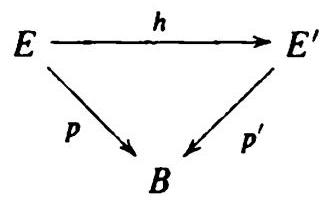
\includegraphics[width=0.3\textwidth]{images/79.0.jpg}
\end{center}
\hspace*{3em} 

Given two covering maps \(p : E \rightarrow  B\) and \({p}^{\prime } : {E}^{\prime } \rightarrow  B\) whose corresponding subgroups \({H}_{0}\) and \({H}_{0}^{\prime }\) are equal, we shall prove that there exists an equivalence \(h\) : \(E \rightarrow  {E}^{\prime }\) . For this purpose, we need to generalize the lifting lemmas of \( \S {54}\) .

\begin{lemma}[The \index{General lifting lemma}general lifting lemma]
	Let \(p : E \rightarrow  B\) be a covering map; let \(p\left( {e}_{0}\right)  = {b}_{0}\) . Let \(f : Y \rightarrow  B\) be a continuous map, with \(f\left( {y}_{0}\right)  = {b}_{0}\) . Suppose \(Y\) is path connected and locally path connected. The map \(f\) can be lifted to a map \(\widetilde{f} : Y \rightarrow  E\) such that \(\bar{f}\left( {y}_{0}\right)  = {e}_{0}\) if and only if

\[
{f}_{ * }\left( {{\pi }_{1}\left( {Y,{y}_{0}}\right) }\right)  \subset  {p}_{ * }\left( {{\pi }_{1}\left( {E,{e}_{0}}\right) }\right) .
\]

Furthermore, if such a lifting exists, it is unique.
\end{lemma}

\begin{proof}
	If the lifting \(\widetilde{f}\) exists, then
\[
{f}_{ * }\left( {{\pi }_{1}\left( {Y,{Y}_{0}}\right) }\right)  = {p}_{ * }\left( {{\bar{f}}_{ * }\left( {{\pi }_{1}\left( {Y,{y}_{0}}\right) }\right) }\right)  \subset  {p}_{ * }\left( {{\pi }_{1}\left( {E,{e}_{0}}\right) }\right) .
\]

This proves the ``only if'' part of the theorem.

Now we prove that if \(\widetilde{f}\) exists, it is unique. Given \({y}_{1} \in  Y\) , choose a path \(\alpha\) in \(Y\) from \({y}_{0}\) to \({y}_{1}\) . Take the path \(f \circ  \alpha\) in \(B\) and lift it to a path \(\gamma\) in \(E\) beginning at \({e}_{0}\) . If a lifting \(\bar{f}\) of \(f\) exists, then \(\bar{f}\left( {y}_{1}\right)\) must equal the end point \(\gamma \left( 1\right)\) of \(\gamma\) , for \(\bar{f} \circ  \alpha\) is a lifting of \(f \circ  \alpha\) that begins at \({e}_{0}\) , and path liftings are unique.

Finally, we prove the ``if'' part of the theorem. The uniqueness part of the proof gives us a clue how to proceed. Given \({y}_{1} \in  Y\) , choose a path \(\alpha\) in \(Y\) from \({y}_{0}\) to \({y}_{1}\) . Lift the path \(f \circ  \alpha\) to a path \(\gamma\) in \(E\) beginning at \({e}_{0}\) , and define \(\widetilde{f}\left( {y}_{1}\right)  = \gamma \left( 1\right)\) . See Figure 79.1. It is a certain amount of work to show that \(\widetilde{f}\) is well-defined, independent of the choice of \(\alpha\) . Once we prove that, continuity of \(\widetilde{f}\) is proved easily, as we now show.

\begin{center}
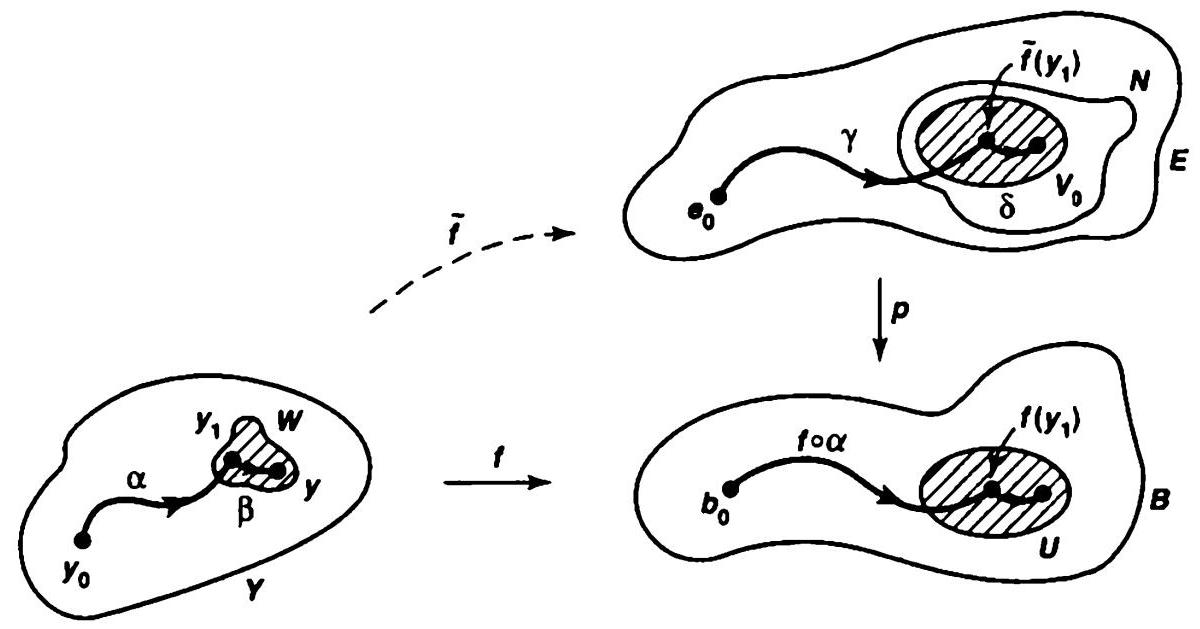
\includegraphics[width=1.0\textwidth]{images/79.1.jpg}
\end{center}
\hspace*{3em} 

Figure 79.1

To prove continuity of \(\widetilde{f}\) at the point \({y}_{1}\) of \(Y\) , we show that, given a neighborhood \(N\) of \(\widetilde{f}\left( {y}_{1}\right)\) , there is a neighborhood \(W\) of \({y}_{1}\) such that \(\widetilde{f}\left( W\right)  \subset  N\) . To begin, choose a path-connected neighborhood \(U\) of \(f\left( {y}_{1}\right)\) that is evenly covered by \(p\) . Break \({p}^{-1}\left( U\right)\) up into slices, and let \({V}_{0}\) be the slice that contains the point \(\widetilde{f}\left( {y}_{1}\right)\) . Replacing \(U\) by a smaller neighborhood of \(f\left( {y}_{1}\right)\) if necessary, we can assume that \({V}_{0} \subset  N\) . Let \({p}_{0} : {V}_{0} \rightarrow  U\) be obtained by restricting \(p\) ; then \({p}_{0}\) is a homeomorphism. Because \(f\) is continuous at \({y}_{1}\) and \(Y\) is locally path connected, we can find a path-connected neighborhood \(W\) of \({y}_{1}\) such that \(f\left( W\right)  \subset  U\) . We shall show that \(\widetilde{f}\left( W\right)  \subset  {V}_{0}\) ; then our result is proved.

Given \(y \in  W\) , choose a path \(\beta\) in \(W\) from \({y}_{1}\) to \(y\) . Since \(\widetilde{f}\) is well defined, \(\widetilde{f}\left( y\right)\) can be obtained by taking the path \(\alpha  * \beta\) from \({y}_{0}\) to \(y\) , lifting the path \(f \circ  \left( {\alpha  * \beta }\right)\) to a path in \(E\) beginning at \({e}_{0}\) , and letting \(\widetilde{f}\left( y\right)\) be the end point of this lifted path. Now \(\gamma\) is a lifting of \(\alpha\) that begins at \({e}_{0}\) . Since the path \(f \circ  \beta\) lies in \(U\) , the path \(\delta  = {p}_{0}^{-1} \circ  f \circ  \beta\) is a lifting of it that begins at \(\widetilde{f}\left( {y}_{1}\right)\) . Then \(\gamma  * \delta\) is a lifting of \(f \circ  \left( {\alpha  * \beta }\right)\) that begins at \({e}_{0}\) ; it ends at the point \(\delta \left( 1\right)\) of \({V}_{0}\) . Hence \(\bar{f}\left( W\right)  \subset  {V}_{0}\) , as desired.

Finally, we show \(\bar{f}\) is well defined. Let \(\alpha\) and \(\beta\) be two paths in \(Y\) from \({y}_{0}\) to \({y}_{1}\) . We must show that if we lift \(f \circ  \alpha\) and \(f \circ  \beta\) to paths in \(E\) beginning at \({e}_{0}\) , then these lifted paths end at the same point of \(E\) .

First, we lift \(f \circ  \alpha\) to a path \(\gamma\) in \(E\) beginning at \({e}_{0}\) ; then we lift \(f \circ  \bar{\beta }\) to a path \(\delta\) in \(E\) beginning at the end point \(\gamma \left( 1\right)\) of \(\gamma\) . Then \(\gamma  * \delta\) is a lifting of the loop \(f \circ  \left( {\alpha  * \bar{\beta }}\right)\) . Now by hypothesis,

\[
{f}_{ * }\left( {{\pi }_{1}\left( {Y,{y}_{0}}\right) }\right)  \subset  {p}_{ * }\left( {{\pi }_{1}\left( {E,{e}_{0}}\right) }\right) .
\]

Hence \(\left\lbrack  {f \circ  \left( {\alpha  * \bar{\beta }}\right) }\right\rbrack\) belongs to the image of \({p}_{ * }\) . Theorem 54.6 now implies that its lift \(\gamma  * \delta\) is a loop in \(E\) .

It follows that \(\bar{f}\) is well defined. For \(\bar{\delta }\) is a lifting of \(f \circ  \beta\) that begins at \({e}_{0}\) , and \(\gamma\) is a lifting of \(f \circ  \alpha\) that begins at \({e}_{0}\) , and both liftings end at the same point of \(E\) .
\end{proof}
\begin{theorem}
	Let \(p : E \rightarrow  B\) and \({p}^{\prime } : {E}^{\prime } \rightarrow  B\) be covering maps; let \(p\left( {e}_{0}\right)  =\)  \({p}^{\prime }\left( {e}_{0}^{\prime }\right)  = {b}_{0}\) . There is an equivalence \(h : E \rightarrow  {E}^{\prime }\) such that \(h\left( {e}_{0}\right)  = {e}_{0}^{\prime }\) if and only if the groups

\[
{H}_{0} = {p}_{ * }\left( {{\pi }_{1}\left( {E,{e}_{0}}\right) }\right) \;\text{ and }\;{H}_{0}^{\prime } = {p}_{ * }^{\prime }\left( {{\pi }_{1}\left( {{E}^{\prime },{e}_{0}^{\prime }}\right) }\right)
\]

are equal. If \(h\) exists, it is unique.
\end{theorem}

\begin{proof}
	We prove the ``only if'' part of the theorem. Given \(h\) , the fact that \(h\) is a homeomorphism implies that
\[
{h}_{ * }\left( {{\pi }_{1}\left( {E,{e}_{0}}\right) }\right)  = {\pi }_{1}\left( {{E}^{\prime },{e}_{0}^{\prime }}\right) .
\]

Since \({p}^{\prime } \circ  h = p\) , we have \({H}_{0} = {H}_{0}^{\prime }\) .

Now we prove the ``if'' part of the theorem; we assume that \({H}_{0} = {H}_{0}^{\prime }\) and show that \(h\) exists. We shall apply the preceding lemma (four times!). Consider the maps

\begin{center}
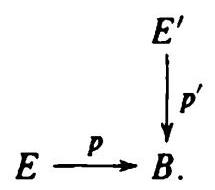
\includegraphics[width=0.2\textwidth]{images/79.11.jpg}
\end{center}
\hspace*{3em} 

Because \({p}^{\prime }\) is a covering map and \(E\) is path connected and locally path connected, there exists a map \(h : E \rightarrow  {E}^{\prime }\) with \(h\left( {e}_{0}\right)  = {e}_{0}^{\prime }\) that is a lifting of \(p\) (that is, such that \(\left. {{p}^{\prime } \circ  h = p}\right)\) . Reversing the roles of \(E\) and \({E}^{\prime }\) in this argument, we see there is a map \(k : {E}^{\prime } \rightarrow  E\) with \(k\left( {e}_{0}^{\prime }\right)  = {e}_{0}\) such that \(p \circ  k = {p}^{\prime }\) . Now consider the maps The map \(k \circ  h : E \rightarrow  E\) is a lifting of \(p\) (since \(p \circ  k \circ  h = {p}^{\prime } \circ  h = p\) ), with \(p\left( {e}_{0}\right)  = {e}_{0}\) . The identity map \({i}_{E}\) of \(E\) is another such lifting. The uniqueness part of the preceding lemma implies that \(k \circ  h = {i}_{E}\) . A similar argument shows that \(h \circ  k\) equals the identity map of \({E}^{\prime }\) .

\begin{center}
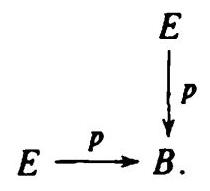
\includegraphics[width=0.2\textwidth]{images/79.12.jpg}
\end{center}
\hspace*{3em} 

We seem to have solved our equivalence problem. But there is a somewhat subtle point we have overlooked. We have obtained a necessary and sufficient condition for there to exist an equivalence \(h \cdot  E \rightarrow  {E}^{\prime }\) that carries the point \({e}_{0}\) to the point \({e}_{0}^{\prime }\) . But we have not yet determined under what conditions there exists an equivalence in general. It is possible that there may be no equivalence carrying \({e}_{0}\) to \({e}_{0}^{\prime }\) but that there is an equivalence carrying \({e}_{0}\) to some other point \({e}_{1}^{\prime }\) of \({\left( {p}^{\prime }\right) }^{-1}\left( {b}_{0}\right)\) . Can we determine whether this is the case merely by examining the subgroups \({H}_{0}\) and \({H}_{0}^{\prime }\) ? We consider this problem now.

If \({H}_{1}\) and \({H}_{2}\) are subgroups of a group \(G\) , you may recall from algebra that they are said to be \index{Conjugate subgroups}conjugate subgroups if \({H}_{2} = \alpha  \cdot  {H}_{1} \cdot  {\alpha }^{-1}\) for some element \(\alpha\) of \(G\) . Said differently, they are conjugate if the isomorphism of \(G\) with itself that maps \(x\) to \(\alpha  \cdot  x \cdot  {\alpha }^{-1}\) carries the group \({H}_{1}\) onto the group \({H}_{2}\) . It is easy to check that conjugacy is an equivalence relation on the collection of subgroups of \(G\) . The equivalence class of the subgroup \(H\) is called the \index{Conjugacy class}conjugacy class of \(H\) .
\end{proof}
\begin{lemma}
	Let \(p : E \rightarrow  B\) be a covering map. Let \({e}_{0}\) and \({e}_{1}\) be points of \({p}^{-1}\left( {b}_{0}\right)\) , and let \({H}_{i} = {p}_{ * }\left( {{\pi }_{1}\left( {E,{e}_{i}}\right) }\right)\) .
\end{lemma}

(a) If \(\gamma\) is a path in \(E\) from \({e}_{0}\) to \({e}_{1}\) , and \(\alpha\) is the loop \(p \circ  \gamma\) in \(B\) , then the equation \(\left\lbrack  \alpha \right\rbrack * {H}_{1} * {\left\lbrack  \alpha \right\rbrack  }^{-1} = {H}_{0}\) holds; hence \({H}_{0}\) and \({H}_{1}\) are conjugate.

(b) Conversely, given \({e}_{0}\) , and given a subgroup \(H\) of \({\pi }_{1}\left( {B,{b}_{0}}\right)\) conjugate to \({H}_{0}\) , there exists a point \({e}_{1}\) of \({p}^{-1}\left( {b}_{0}\right)\) such that \({H}_{1} = H\) .

\begin{proof}
	(a) First, we show that \(\left\lbrack  \alpha \right\rbrack * {H}_{1} * {\left\lbrack  \alpha \right\rbrack  }^{-1} \subset  {H}_{0}\) . Given an element \(\left\lbrack  h\right\rbrack\) of \({H}_{1}\) , we have \(\left\lbrack  h\right\rbrack = {p}_{ * }\left( \left\lbrack  \widetilde{h}\right\rbrack  \right)\) for some loop \(\widetilde{h}\) in \(E\) based at \({e}_{1}\) . Let \(\widetilde{k}\) be the path \(\widetilde{k} = \left( {\gamma  * \widetilde{h}}\right)  * \widetilde{\gamma }\) ; it is a loop in \(E\) based at \({e}_{0}\) , and
\[
{p}_{ * }\left( \left\lbrack  \bar{k}\right\rbrack  \right)  = \left\lbrack  {\left( {\alpha  * h}\right)  * \bar{\alpha }}\right\rbrack = \left\lbrack  \alpha \right\rbrack * \left\lbrack  h\right\rbrack * {\left\lbrack  \alpha \right\rbrack  }^{-1},
\]

so the latter element belongs to \({p}_{ * }\left( {{\pi }_{1}\left( {E,{e}_{0}}\right) }\right)  = {H}_{0}\) , as desired. See Figure 79.2.

Now we show that \(\left\lbrack  \alpha \right\rbrack * {H}_{1} * {\left\lbrack  \alpha \right\rbrack  }^{-1} \supset  {H}_{0}\) . Note that \(\bar{\gamma }\) is a path from \({e}_{1}\) to \({e}_{0}\) and \(\bar{\alpha }\) equals the loop \(p \circ  \bar{\gamma }\) . By the result just proved, we have

\[
\left\lbrack  \bar{\alpha }\right\rbrack * {H}_{0} * {\left\lbrack  \bar{\alpha }\right\rbrack  }^{-1} \subset  {H}_{1}
\]

which implies out desired result.

(b) To prove the converse, let \({e}_{0}\) be given and let \(H\) be conjugate to \({H}_{0}\) . Then \({H}_{0} = \left\lbrack  \alpha \right\rbrack * H * {\left\lbrack  \alpha \right\rbrack  }^{-1}\) for some loop \(\alpha\) in \(B\) based at \({b}_{0}\) . Let \(\gamma\) be the lifting of \(\alpha\) to a path in \(E\) beginning at \({e}_{0}\) , and let \({e}_{1} = \gamma \left( 1\right)\) . Then (a) implies that \({H}_{0} = \left\lbrack  \alpha \right\rbrack * {H}_{1} * {\left\lbrack  \alpha \right\rbrack  }^{-1}\) . We conclude that \(H = {H}_{1}\) .

\begin{center}
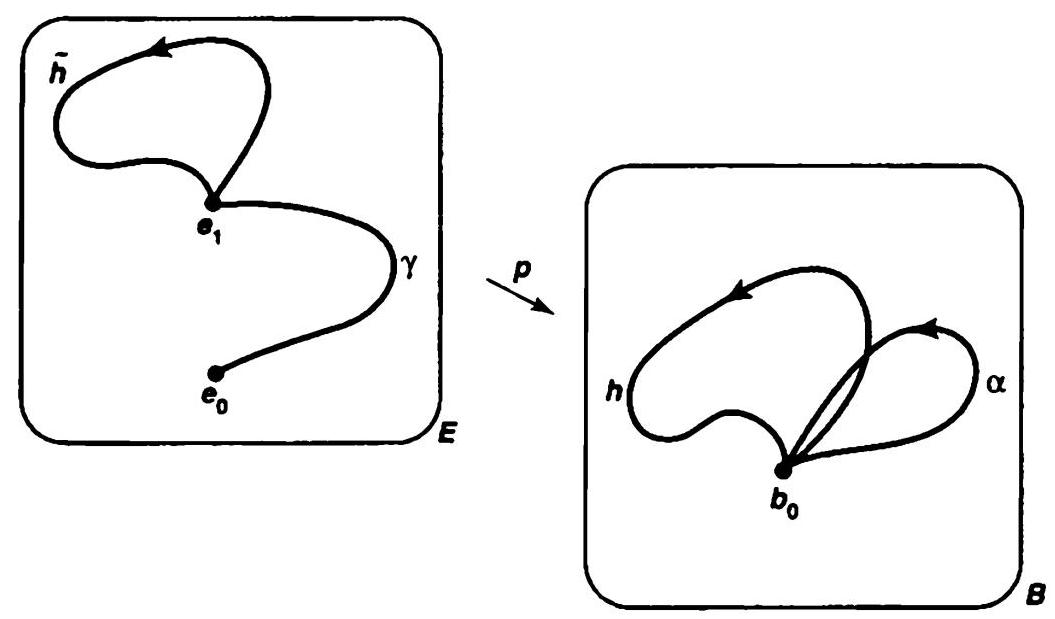
\includegraphics[width=0.9\textwidth]{images/79.2.jpg}
\end{center}
\hspace*{3em} 

Figure 79.2
\end{proof}
\begin{theorem}
	Let \(p : E \rightarrow  B\) and \({p}^{\prime } : {E}^{\prime } \rightarrow  B\) be covering maps; let \(p\left( {e}_{0}\right)  =\)  \({p}^{\prime }\left( {e}_{0}^{\prime }\right)  = {b}_{0}\) . The covering maps \(p\) and \({p}^{\prime }\) are equivalent if and only if the subgroups

\[
{H}_{0} = {p}_{ * }\left( {{\pi }_{1}\left( {E,{e}_{0}}\right) }\right) \;\text{ and }\;{H}_{0}^{\prime } = {p}_{ * }^{\prime }\left( {{\pi }_{1}\left( {{E}^{\prime },{e}_{0}^{\prime }}\right) }\right)
\]

of \({\pi }_{1}\left( {B,{b}_{0}}\right)\) are conjugate.
\end{theorem}

\begin{proof}
	If \(h : E \rightarrow  {E}^{\prime }\) is an equivalence, let \({e}_{1}^{\prime } = h\left( {e}_{0}\right)\) , and let \({H}_{1}^{\prime } = {p}_{ * }\left( {{\pi }_{1}\left( {{E}^{\prime },{e}_{1}^{\prime }}\right) }\right)\) Theorem 79.2 implies that \({H}_{0} = {H}_{1}^{\prime }\) , while the preceding lemma tells us that \({H}_{1}^{\prime }\) is conjugate to \({H}_{0}^{\prime }\) .
Conversely, if the groups \({H}_{0}\) and \({H}_{0}^{\prime }\) are conjugate, the preceding lemma implies there is a point \({e}_{1}^{\prime }\) of \({E}^{\prime }\) such that \({H}_{1}^{\prime } = {H}_{0}\) . Theorem 79.2 then gives us an equivalence \(h : E \rightarrow  {E}^{\prime }\) such that \(h\left( {e}_{0}\right)  = {e}_{1}^{\prime }\) .

\begin{centeredblock}
\begin{example}
	Consider covering spaces of the circle \(B = {S}^{1}\) . Because \({\pi }_{1}\left( {B,{b}_{0}}\right)\) is abelian, two subgroups of \({\pi }_{1}\left( {B,{b}_{0}}\right)\) are conjugate if and only if they are equal. Therefore two coverings of \(B\) are equivalent if and only if they correspond to the same subgroup of \({\pi }_{1}\left( {B,{b}_{0}}\right)\) .

Now \({\pi }_{1}\left( {B,{b}_{0}}\right)\) is isomorphic to the integers \(\mathbb{Z}\) . What are the subgroups of \({\mathbb{Z}}^{2}\) It is standard theorem of modern algebra that, given a nontrivial subgroup of \(\mathbb{Z}\) , it must be the group \({G}_{n}\) consisting of all multiples of \(n\) , for some \(n \in  {\mathbb{Z}}_{ + }\) .

We have studied one covering space of the circle, the covering \(p : \mathbb{R} \rightarrow  {S}^{1}\) It must correspond to the trivial subgroup of \({\pi }_{1}\left( {{S}^{1},{b}_{0}}\right)\) , because \(\mathbb{R}\) is simply connected We have also considered the covering \(p : {S}^{1} \rightarrow  {S}^{1}\) defined by \(p\left( z\right)  = {z}^{n}\) , where \(z\) is a complex number. In this case, the map \({p}_{ * }\) carries a generator of \({\pi }_{1}\left( {{S}^{1},{b}_{0}}\right)\) into \(n\) times itself. Therefore, the group \({p}_{ * }\left( {{\pi }_{1}\left( {{S}^{1},{b}_{0}}\right) }\right)\) corresponds to the subgroup \({G}_{n}\) of \(\mathbb{Z}\) under the standard isomorphism of \({\pi }_{1}\left( {{S}^{1},{b}_{0}}\right)\) with \(\mathbb{Z}\) .

We conclude from the preceding theorem that every path-connected covering space of \({S}^{1}\) is equivalent to one of these coverings.
\end{example}
\end{centeredblock}
\end{proof}
\section*{Exercises}
\begin{enumerate}[itemsep=0.4em, parsep=0pt, topsep=0pt, partopsep=0pt, leftmargin=*, label=\arabic*., ref=\arabic*]
\item Show that if \(n > 1\) , every continuous map \(f : {S}^{n} \rightarrow  {S}^{1}\) is nulhomotopic. [Hint: Use the lifting lemma.]
\item
  \begin{enumerate}[itemsep=0.2em, parsep=0pt, topsep=0pt, partopsep=0pt, leftmargin=*, label=(\alph*), align=left]
  \item Show that every continuous map \(f : {P}^{2} \rightarrow  {S}^{1}\) is nulhomotopic.

  \item Find a continuous map of the torus into \({S}^{1}\) that is not nulhomotopic.
  \end{enumerate}
\item Let \(p : E \rightarrow  B\) be a covering map; let \(p\left( {e}_{0}\right)  = {b}_{0}\) . Show that \({H}_{0} =\)  \({p}_{ * }\left( {{\pi }_{1}\left( {E,{e}_{0}}\right) }\right)\) is a normal subgroup of \({\pi }_{1}\left( {B,{b}_{0}}\right)\) if and only if for every pair of points \({e}_{1},{e}_{2}\) of \({p}^{-1}\left( {b}_{0}\right)\) , there is an equivalence \(h : E \rightarrow  E\) with \(h\left( {e}_{1}\right)  = {e}_{2}\) .
\item Let \(T = {S}^{1} \times  {S}^{1}\) , the torus. There is an isomorphism of \({\pi }_{1}\left( {T,{b}_{0} \times  {b}_{0}}\right)\) with \(\mathbb{Z} \times  \mathbb{Z}\) induced by projections of \(T\) onto its two factors.
  \begin{enumerate}[itemsep=0.2em, parsep=0pt, topsep=0pt, partopsep=0pt, leftmargin=*, label=(\alph*), align=left]
  \item Find a covering space of \(T\) corresponding to the subgroup of \(\mathbb{Z} \times  \mathbb{Z}\) generated by the element \(m \times  0\) , where \(m\) is a positive integer.
  \item Find a covering space of \(T\) corresponding to the trivial subgroup of \(\mathbb{Z} \times  \mathbb{Z}\) .
  \item Find a covering space of \(T\) corresponding to the subgroup of \(\mathbb{Z} \times  \mathbb{Z}\) generated by \(m \times  0\) and \(0 \times  n\) , where \(m\) and \(n\) are positive integers. *5. Let \(T = {S}^{1} \times  {S}^{1}\) be the torus; let \({x}_{0} = {b}_{0} \times  {b}_{0}\) .
  \item Prove the following: \textsl{Theorem.} Every isomorphism of \({\pi }_{1}\left( {T,{x}_{0}}\right)\) with itself is induced by a homeomorphism of \(T\) with itself that maps \({x}_{0}\) to \({x}_{0}\) .  [Hint: Let \(p : {\mathbb{R}}^{2} \rightarrow  T\) be the usual covering map. If \(A\) is a \(2 \times  2\) matrix with integer entries, the linear map \({T}_{A} : {\mathbb{R}}^{2} \rightarrow  {\mathbb{R}}^{2}\) with matrix \(A\) induces a continuous map \(f : T \rightarrow  T\) . Furthermore, \(f\) is a homeomorphism if \(A\) is invertible over the integers.]
  \item Prove the following: \textsl{Theorem.} If \(E\) is a covering space of \(T\) , then \(E\) is homeomorphic either to \({\mathbb{R}}^{2}\) , or to \({S}^{1} \times  \mathbb{R}\) , or to \(T\) .  [Hint: You may use the following result from algebra: If \(F\) is a free abelian group of rank 2 and \(N\) is a nontrivial subgroup, then there is a basis \({a}_{1},{a}_{2}\) for \(F\) such that either (1) \(m{a}_{1}\) is a basis for \(N\) , for some positive integer \(m\) , or \(\left( 2\right) m{a}_{1},n{a}_{2}\) is a basis for \(N\) , where \(m\) and \(n\) are positive integers.] *6. Prove the following: \textsl{Theorem.} Let \(G\) be a topological group with multiplication operation \(m : G \times\)  \(G \rightarrow  G\) and identity element \(e\) . Assume \(p : \bar{G} \rightarrow  G\) is a covering map. Given \(\widetilde{e}\) with \(p\left( \widetilde{e}\right)  = e\) , there is a unique multiplication operation on \(\bar{G}\) that makes it into a topological group such that \(\widetilde{e}\) is the identity element and \(p\) is a homomorphism.  Proof. Recall that, by our convention, \(G\) and \(\widetilde{G}\) are path connected and locally path connected.
  \item Let \(I : G \rightarrow  G\) be the map \(I\left( g\right)  = {g}^{-1}\) . Show there exist unique maps \(\bar{m} : \widetilde{G} \times  \widetilde{G} \rightarrow  \widetilde{G}\) and \(\widetilde{I} : \widetilde{G} \rightarrow  \widetilde{G}\) with \(\widetilde{m}\left( {\widetilde{e} \times  \widetilde{e}}\right)  = \widetilde{e}\) and \(\widetilde{I}\left( \bar{e}\right)  = \bar{e}\) such that \(p \circ  \widetilde{m} = m \circ  \left( {p \times  p}\right)\) and \(p \circ  \widetilde{I} = I \circ  p\) .
  \item Show the maps \(\widetilde{G} \rightarrow  \widetilde{G}\) given by \(\widetilde{g} \rightarrow  \widetilde{m}\left( {\widetilde{e} \times  \widetilde{g}}\right)\) and \(\widetilde{g} \rightarrow  \widetilde{m}\left( {\widetilde{g} \times  \widetilde{e}}\right)\) equal the identity map of \(\widetilde{G}\) . [Hint: Use the uniqueness part of Lemma 79.1.]
  \item Show the maps \(\widetilde{G} \rightarrow  \widetilde{G}\) given by \(\widetilde{g} \rightarrow  \widetilde{m}\left( {\widetilde{g} \times  \widetilde{I}\left( \widetilde{g}\right) }\right)\) and \(\widetilde{g} \rightarrow  \widetilde{m}\left( {\widetilde{I}\left( \widetilde{g}\right)  \times  \widetilde{g}}\right)\) map \(\widetilde{G}\) to \(\widetilde{e}\) .
  \item Show the maps \(\bar{G} \times  \widetilde{G} \times  \bar{G} \rightarrow  \bar{G}\) given by \[ \begin{aligned}  & \widetilde{g} \times  {\widetilde{g}}^{\prime } \times  {\widetilde{g}}^{\prime \prime } \rightarrow  \widetilde{m}\left( {\widetilde{g} \times  \bar{m}\left( {{\widetilde{g}}^{\prime } \times  {\widetilde{g}}^{\prime \prime }}\right) }\right) \\  & \widetilde{g} \times  {\widetilde{g}}^{\prime } \times  {\widetilde{g}}^{\prime \prime } \rightarrow  \bar{m}\left( {\widetilde{m}\left( {\widetilde{g} \times  {\widetilde{g}}^{\prime }}\right)  \times  {\widetilde{g}}^{\prime \prime }}\right) \end{aligned} \] are equal.
  \item Complete the proof.
  \end{enumerate}
\item Let \(p : \widetilde{G} \rightarrow  G\) be a homomorphism of topological groups that is a covering map. Show that if \(G\) is abelian, so is \(\bar{G}\) .
\end{enumerate}
\section*{§ 80 The Universal Covering Space}

Suppose \(p : E \rightarrow  B\) is a covering map, with \(p\left( {e}_{0}\right)  = {b}_{0}\) . If \(E\) is simply connected, then \(E\) is called a \index{Universal covering space}universal covering space of \(B\) . Since \({\pi }_{1}\left( {E,{e}_{0}}\right)\) is trivial, this covering space corresponds to the trivial subgroup of \({\pi }_{1}\left( {B,{b}_{0}}\right)\) under the correspondence defined in the preceding section. Theorem 79.4 thus implies that any two universal covering spaces of \(B\) are equivalent. For this reason, we often speak of ``the'' universal covering space of a given space \(B\) . Not every space has a universal covering space, as we shall see. For the moment, we shall simply assume that B has a universal covering space and derive some consequences of this assumption.

We prove two preliminary lemmas:

\begin{lemma}
	Let \(B\) be path connected and locally path connected. Let \(p : E \rightarrow  B\) be a covering map in the former sense (so that \(E\) is not required to be path connected). If \({E}_{0}\) is a path component of \(E\) , then the map \({p}_{0} : {E}_{0} \rightarrow  B\) obtained by restricting \(p\) is a covenng map.
\end{lemma}

\begin{proof}
	We first show \({p}_{0}\) is surjective. Since the space \(E\) is locally homeomorphic to \(B\) , it is locally path connected. Therefore \({E}_{0}\) is open in \(E\) . It follows that \(p\left( {E}_{0}\right)\) is open in \(B\) . We show that \(p\left( {E}_{0}\right)\) is also closed in \(B\) , so that \(p\left( {E}_{0}\right)  = B\) .
Let \(x\) be a point of \(B\) beloriging to the closure of \(p\left( {E}_{0}\right)\) . Let \(U\) be a path-connected neighborhood of \(x\) that is evenly covered by \(p\) . Since \(U\) contains a point of \(p\left( {E}_{0}\right)\) , some slice \({V}_{\alpha }\) of \({p}^{-1}\left( U\right)\) must intersect \({E}_{0}\) . Since \({V}_{\alpha }\) is homeomorphic to \(U\) , it is path connected; therefore it must be contained in \({E}_{0}\) . Then \(p\left( {V}_{\alpha }\right)  = U\) is contained in \(p\left( {E}_{0}\right)\) , so that in particular, \(x \in  p\left( {E}_{0}\right)\) .

Now we show \({p}_{0} : {E}_{0} \rightarrow  B\) is a covering map. Given \(x \in  B\) , choose a neighborhood \(U\) of \(x\) as before. If \({V}_{\alpha }\) is a slice of \({p}^{-1}\left( U\right)\) , then \({V}_{\alpha }\) is path connected; if it intersects \({E}_{0}\) , it lies in \({E}_{0}\) . Therefore, \({p}_{0}^{-1}\left( U\right)\) equals the union of those slices \({V}_{\alpha }\) of \({p}^{-1}\left( U\right)\) that intersect \({E}_{0}\) ; each of these is open in \({E}_{0}\) and is mapped homeomorphi-cally by \({p}_{0}\) onto \(U\) . Thus \(U\) is evenly covered by \({p}_{0}\) .
\end{proof}
\begin{lemma}
	Let \(p,q\) , and \(r\) be continuous maps with \(p = r \circ  q\) , as in the following diagram:

\begin{center}
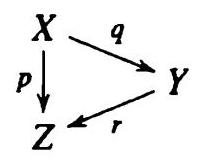
\includegraphics[width=0.2\textwidth]{images/80.01.jpg}
\end{center}
\hspace*{3em} 

(a) If \(p\) and \(q\) are covering maps, so is \(q\) .

*(b) If \(p\) and \(q\) are covering maps, so is \(r\) .
\end{lemma}

\begin{proof}
	By our convention, \(X,Y\) , and \(Z\) are path connected and locally path connected. Let \({x}_{0} \in  X\) ; set \({y}_{0} = q\left( {x}_{0}\right)\) and \({z}_{0} = p\left( {x}_{0}\right)\) .
(a) Assume that \(p\) and \(r\) are covering maps. We show first that \(q\) is surjective. Given \(y \in  Y\) , choose a path \(\bar{\alpha }\) in \(Y\) from \({y}_{0}\) to \(y\) . Then \(\alpha  = r \circ  \bar{\alpha }\) is a path in \(Z\) beginning at \({z}_{0}\) ; let \(\widetilde{\bar{\alpha }}\) be a lifting of \(\alpha\) to a path in \(X\) beginning at \({x}_{0}\) . Then \(q \circ  \widetilde{\bar{\alpha }}\) is a lifting of \(\alpha\) to \(Y\) that begins at \({y}_{0}\) . By uniqueness of path liftings, \(\widetilde{\alpha } = q \circ  \widetilde{\bar{\alpha }}\) . Then \(q\) maps the end point of \(\overline{\bar{\alpha }}\) to the end point \(y\) of \(\bar{\alpha }\) . Thus \(q\) is surjective.

Given \(y \in  Y\) , we find a neighborhood of \(y\) that is evenly covered by \(q\) . Let \(z =\)  \(r\left( y\right)\) . Since \(p\) and \(r\) are covering maps, we can find a path-connected neighborhood \(U\) of \(z\) that is evenly covered by both \(p\) and \(r\) . Let \(V\) be the slice of \({r}^{-1}\left( U\right)\) that contains the point \(y\) ; we show \(V\) is evenly covered by \(q\) . Let \(\left\{  {U}_{\alpha }\right\}\) be the collection of slices of \({p}^{-1}\left( U\right)\) . Now \(q\) maps each set \({U}_{\alpha }\) into the set \({r}^{-1}\left( U\right)\) ; because \({U}_{\alpha }\) is connected, it must be mapped by \(q\) into a single one of the slices of \({r}^{-1}\left( U\right)\) . Therefore, \({q}^{-1}\left( V\right)\) equals the union of those slices \({U}_{\alpha }\) that are mapped by \(q\) into \(V\) . It is easy to see that each such \({U}_{\alpha }\) is mapped homeomorphically onto \(V\) by \(q\) . For let \({p}_{0},{q}_{0},{r}_{0}\) be the maps obtained by restricting \(p,q\) , and \(r\) , respectively, as indicated in the following diagram:

\begin{center}
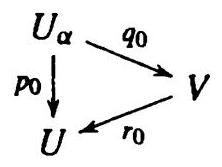
\includegraphics[width=0.2\textwidth]{images/80.02.jpg}
\end{center}
\hspace*{3em} 

Because \({p}_{0}\) and \({r}_{0}\) are homeomorphisms, so is \({q}_{0} = {r}_{0}^{-1} \circ  {p}_{0}\) .

*(b) We shall use this result only in the exercises. Assume that \(p\) and \(q\) are covering maps. Because \(p = r \circ  q\) and \(p\) is surjective, \(r\) is also surjective.

Given \(z \in  Z\) , let \(U\) be a path-connected neighborhood of \(z\) that is evenly covered by \(p\) . We show that \(U\) is also evenly covered by \(r\) . Let \(\left\{  {V}_{\beta }\right\}\) be the collection of path components of \({r}^{-1}\left( U\right)\) ; these sets are disjoint and open in \(Y\) . We show that for each \(\beta\) , the map \(r\) carries \({V}_{\beta }\) homeomorphically onto \(U\) .

Let \(\left\{  {U}_{\alpha }\right\}\) be the collection of slices of \({p}^{-1}\left( U\right)\) ; they are disjoint, open, and path connected, so they are the path components of \({p}^{-1}\left( U\right)\) . Now \(q\) maps each \({U}_{\alpha }\) into the set \({r}^{-1}\left( U\right)\) ; because \({U}_{\alpha }\) is connected, it must be mapped by \(q\) into one of the sets \({V}_{\beta }\) . Therefore \({q}^{-1}\left( {V}_{\beta }\right)\) equals the union of a subcollection of the collection \(\left\{  {U}_{\alpha }\right\}\) . Theorem 53.2 and Lemma 80.1 together imply that if \({U}_{{\alpha }_{0}}\) is any one of the path components of \({q}^{-1}\left( {V}_{\beta }\right)\) then the map \({q}_{0} : {U}_{{\alpha }_{0}} \rightarrow  {V}_{\beta }\) obtained by restricting \(q\) is a covering map. In particular, \({q}_{0}\) is surjective. Hence \({q}_{0}\) is a homeomorphism, being continuous, open, and injective as well. Consider the maps

\begin{center}
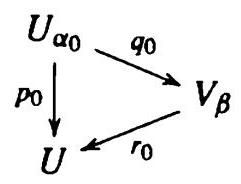
\includegraphics[width=0.2\textwidth]{images/80.03.jpg}
\end{center}
\hspace*{3em} 

obtained by restricting \(p,q\) , and \(r\) . Because \({p}_{0}\) and \({q}_{0}\) are homeomorphisms, so is \({r}_{0}\) .
\end{proof}
\begin{theorem}
	Let \(p : E \rightarrow  B\) be a covering map, with \(E\) simply connected. Given any covering map \(r : Y \rightarrow  B\) , there is a covering map \(q : E \rightarrow  Y\) such that \(r \circ  q = p\) .
\end{theorem}

\begin{center}
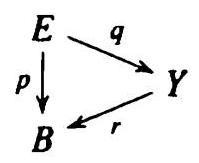
\includegraphics[width=0.2\textwidth]{images/80.04.jpg}
\end{center}
\hspace*{3em} 

This theorem shows why \(E\) is called a universal covering space of \(B\) ; it covers every other covering space of \(B\) .

\begin{proof}
	Let \({b}_{0} \in  B\) ; choose \({e}_{0}\) and \({y}_{0}\) so that \(p\left( {e}_{0}\right)  = {b}_{0}\) and \(r\left( {y}_{0}\right)  = {b}_{0}\) . We apply Lemma 79.1 to construct \(q\) . The map \(r\) is a covering map, and the condition
\[
{p}_{ * }\left( {{\pi }_{1}\left( {E,{e}_{0}}\right) }\right)  \subset  {r}_{ * }\left( {{\pi }_{1}\left( {Y,{y}_{0}}\right) }\right)
\]

is satisfied trivially because \(E\) is simply connected. Therefore, there is a map \(q : E \rightarrow\)  \(Y\) such that \(r \circ  q = p\) and \(q\left( {e}_{0}\right)  = {y}_{0}\) . It follows from the preceding lemma that \(q\) is a covering map.

Now we give an example of a space that has no universal covering space. We need the following lemma.
\end{proof}
\begin{lemma}
	Let \(p : E \rightarrow  B\) be a covering map; let \(p\left( {e}_{0}\right)  = {b}_{0}\) . If \(E\) is simply connected, then \({b}_{0}\) has a neighborhood \(U\) such that inclusion \(i : U \rightarrow  B\) induces the trivial homomorphism

\[
{i}_{ * } : {\pi }_{1}\left( {U,{b}_{0}}\right)  \rightarrow  {\pi }_{1}\left( {B,{b}_{0}}\right) .
\]
\end{lemma}

\begin{proof}
	Let \(U\) be a neighborhood of \({b}_{0}\) that is evenly covered by \(p\) ; break \({p}^{-1}\left( U\right)\) up into slices; let \({U}_{\alpha }\) be the slice containing \({e}_{0}\) . Let \(f\) be a loop in \(U\) based at \({b}_{0}\) . Because \(p\) defines a homeomorphism of \({U}_{\alpha }\) with \(U\) , the loop \(f\) lifts to a loop \(\widetilde{f}\) in \({U}_{\alpha }\) based at \({e}_{0}\) . Since \(E\) is simply connected, there is a path homotopy \(\widetilde{F}\) in \(E\) between \(\widetilde{f}\) and a constant loop. Then \(p \circ  \widetilde{F}\) is a path homotopy in \(B\) between \(f\) and a constant loop.
\begin{centeredblock}
\begin{example}
	Let \(X\) be our familiar ``infinite earring'' in the plane, if \({C}_{n}\) is the circle of radius \(1/n\) in the plane with center at the point \(\left( {1/n,0}\right)\) , then \(X\) is the union of the curcles \({C}_{n}\) . Let \({b}_{0}\) be the origin; we show that if \(U\) is any neighborhood of \({b}_{0}\) in \(X\) , then the homomorphism of fundamental groups induced by inclusion \(i : U \rightarrow  X\) is not trivial.

Given \(n\) , there is a retr\index{fixed-point-free action@Fixed-point-free action}Fixed-point-free action action \(r : X \rightarrow  {C}_{n}\) obtained by lettung \(r\) map each circle \({C}_{t}\) for \(i \neq  n\) to the point \({b}_{0}\) . Choose \(n\) large enough that \({C}_{n}\) lies in \(U\) . Then in the following diagram of homomorphisms induced by inclusion, \({j}_{ * }\) is injective, hence \({i}_{ * }\) cannot be trivial.

\begin{center}
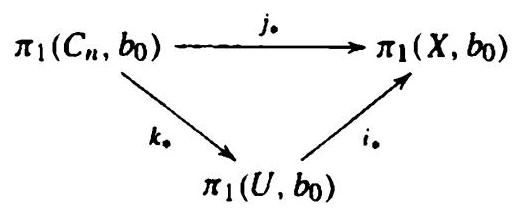
\includegraphics[width=0.4\textwidth]{images/80.05.jpg}
\end{center}
\hspace*{3em}

It follows that even though \(X\) is path connected and locally path connected, it has no universal covering space.
\end{example}
\end{centeredblock}
\end{proof}
\section*{Exercise}

1. Let \(q : X \rightarrow  Y\) and \(r : Y \rightarrow  Z\) be maps; let \(p = r \circ  q\) .

(a) Let \(q\) and \(r\) be covering maps. Show that if \(Z\) has a universal covering space, then \(p\) is a covering map. Compare Exercise 4 of  \S 53.

*(b) Give an example where \(q\) and \(r\) are covering maps but \(p\) is not.

\section*{*§  81 Covering Transformations}

Given a covering map \(p : E \rightarrow  B\) , it is of some interest to consider the set of all equivalences of this covering space with itself. Such an equivalence is called a \index{Covering transformation}covering transformation. Composites and inverses of covering transformations are covering transformations, so this set forms a group; it is called the \index{Group of covering transformations}group of covering transformations and denoted \(\mathcal{C}\left( {E,p,B}\right)\) .

Throughout this section, we shall assume that \(p : E \rightarrow  B\) is a covering map with \(p\left( {e}_{0}\right)  = {b}_{0}\) ; and we shall let \({H}_{0} = {p}_{ * }\left( {{\pi }_{1}\left( {E,{e}_{0}}\right) }\right)\) . We shall show that the group \(\mathcal{C}\left( {E,p,B}\right)\) is completely determined by the group \({\pi }_{1}\left( {B,{b}_{0}}\right)\) and the subgroup \({H}_{0}\) . Specifically, we shall show that if \(N\left( {H}_{0}\right)\) is the largest subgroup of \({\pi }_{1}\left( {B,{b}_{0}}\right)\) of which \({H}_{0}\) is a normal subgroup, then \(\mathcal{C}\left( {E,p,B}\right)\) is isomorphic to \(N\left( {H}_{0}\right) /{H}_{0}\) .

We define \(N\left( {H}_{0}\right)\) formally as follows:

\begin{definition}
	If \(H\) is a subgroup of the group \(G\) , then the \index{Normalizer}normalizer of \(H\) in \(G\) is the subset of \(G\) defined by the equation

\[
N\left( H\right)  = \left\{  {g \mid  {gH}{g}^{-1} = H}\right\}  .
\]
\end{definition}

It is easy to see that \(N\left( H\right)\) is a subgroup of \(G\) . It follows from the definition that it contains \(H\) as a normal subgroup and is the largest such subgroup of \(G\) .

The correspondence between the groups \(N\left( {H}_{0}\right) /{H}_{0}\) and \(\mathcal{C}\left( {E,p,B}\right)\) is established by using the lifting correspondence of \( \S {54}\) and the results about the existence of equivalences proved in \( \S {79}\) . We make the following definition:

\begin{definition}
	Given \(p : E \rightarrow  B\) with \(p\left( {e}_{0}\right)  = {b}_{0}\) , let \(F\) be the set \(F = {p}^{-1}\left( {e}_{0}\right)\) . Let

\[
\Phi  : {\pi }_{1}\left( {B,{b}_{0}}\right) /{H}_{0} \rightarrow  F
\]

be the lifting correspondence of Theorem 54.6; it is a bijection. Define also a correspondence

\[
\Psi  : \mathcal{C}\left( {E,p,B}\right)  \rightarrow  F
\]

by setting \(\Psi \left( h\right)  = h\left( {e}_{0}\right)\) for each covering transformation \(h : E \rightarrow  E\) . Since \(h\) is uniquely determined once its value at \({e}_{0}\) is known, the correspondence \(\Psi\) is injective.
\end{definition}

\begin{lemma}
	The image of the map \(\Psi\) equals the image under \(\Phi\) of the subgroup \(N\left( {H}_{0}\right) /{H}_{0}\) of \({\pi }_{1}\left( {B,{b}_{0}}\right) /{H}_{0}\) .
\end{lemma}

\begin{proof}
	Recall that the lifting correspondence \(\phi  : {\pi }_{1}\left( {B,{b}_{0}}\right)  \rightarrow  F\) is defined as follows: Given a loop \(\alpha\) in \(B\) at \({b}_{0}\) , let \(\gamma\) be its lift to \(E\) beginning at \({e}_{0}\) ; let \({e}_{1} = \gamma \left( 1\right)\) ; and define \(\phi\) by setting \(\phi \left( \left\lbrack  \alpha \right\rbrack  \right)  = {e}_{1}\) . To prove the lemma, we need to show that there is a covering transformation \(h : E \rightarrow  E\) with \(h\left( {e}_{0}\right)  = {e}_{1}\) if and only if \(\left\lbrack  \alpha \right\rbrack \in  N\left( {H}_{0}\right)\) .
This is easy. Lemma 79.1 tells us that \(h\) exists if and only if \({H}_{0} = {H}_{1}\) , where \({H}_{1} = {p}_{ * }\left( {{\pi }_{1}\left( {E,{e}_{1}}\right) }\right)\) . And Lemma 79.3 tells us that \(\left\lbrack  \alpha \right\rbrack * {H}_{1} * {\left\lbrack  \alpha \right\rbrack  }^{-1} = {H}_{0}\) . Hence \(h\) exists if and only if \(\left\lbrack  \alpha \right\rbrack * {H}_{0} * {\left\lbrack  \alpha \right\rbrack  }^{-1} = {H}_{0}\) , which is simply the statement that \(\left\lbrack  \alpha \right\rbrack \in\)  \(N\left( {H}_{0}\right)\) .
\end{proof}
\begin{theorem}
	The bijection

\[
{\Phi }^{-1} \circ  \Psi  : \mathcal{C}\left( {E,p,B}\right)  \rightarrow  N\left( {H}_{0}\right) /{H}_{0}
\]

is an isomorphism of groups.
\end{theorem}

\begin{proof}
	We need only show that \({\Phi }^{-1} \circ  \Psi\) is a homomorphism. Let \(h,k : E \rightarrow  E\) be covering transformations. Let \(h\left( {e}_{0}\right)  = {e}_{1}\) and \(k\left( {e}_{0}\right)  = {e}_{2}\) ; then
\[
\Psi \left( h\right)  = {e}_{1}\;\text{ and }\;\Psi \left( k\right)  = {e}_{2},
\]

by definition. Choose paths \(\gamma\) and \(\delta\) in \(E\) from \({e}_{0}\) to \({e}_{1}\) and \({e}_{2}\) , respectively. If \(\alpha  = p \circ  \gamma\) and \(\beta  = p \circ  \delta\) , then

\[
\Phi \left( {\left\lbrack  \alpha \right\rbrack  {H}_{0}}\right)  = {e}_{1}\;\text{ and }\;\Phi \left( {\left\lbrack  \beta \right\rbrack  {H}_{0}}\right)  = {e}_{2},
\]

by definition. Let \({e}_{3} = h\left( {k\left( {e}_{0}\right) }\right)\) ; then \(\Psi \left( {h \circ  k}\right)  = {e}_{3}\) . We show that

\[
\Phi \left( {\left\lbrack  {\alpha  * \beta }\right\rbrack  {H}_{0}}\right)  = {e}_{3},
\]

and the proof is complete.

Since \(\delta\) is a path from \({e}_{0}\) to \({e}_{2}\) , the path \(h \circ  \delta\) is a path from \(h\left( {e}_{0}\right)  = {e}_{1}\) to \(h\left( {e}_{2}\right)  = h\left( {k\left( {e}_{0}\right) }\right)  = {e}_{3}\) . See Figure 81.1. Then the product \(\gamma  * \left( {h \circ  \delta }\right)\) is defined and is a path from \({e}_{0}\) to \({e}_{3}\) . It is a lifting of \(\alpha  * \beta\) , since \(p \circ  \gamma  = \alpha\) and \(p \circ  h \circ  \delta  = p \circ  \delta  = \beta\) . Therefore \(\Phi \left( {\left\lbrack  {\alpha  * \beta }\right\rbrack  {H}_{0}}\right)  = {e}_{3}\) , as desired.

\begin{center}
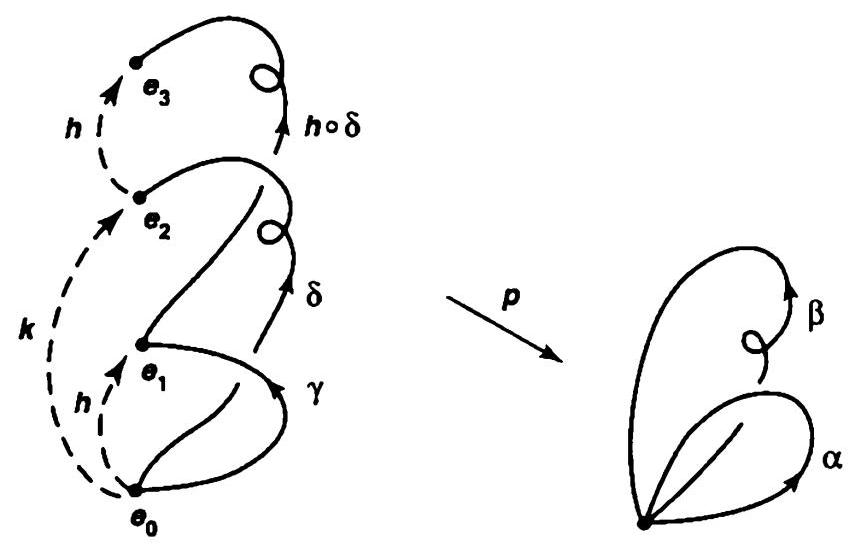
\includegraphics[width=0.7\textwidth]{images/81.1.jpg}
\end{center}
\hspace*{3em} 

Figure 81.1
\end{proof}
\begin{corollary}
	The group \({H}_{0}\) is a normal subgroup of \({\pi }_{1}\left( {B,{b}_{0}}\right)\) if and only if for every pair of points \({e}_{1}\) and \({e}_{2}\) of \({p}^{-1}\left( {b}_{0}\right)\) , there is a covering transformation \(h : E \rightarrow\)  \(E\) with \(h\left( {e}_{1}\right)  = {e}_{2}\) . In this case, there is an isomorphism

\[
{\Phi }^{-1} \circ  \Psi  : \mathcal{C}\left( {E,p,B}\right)  \rightarrow  {\pi }_{1}\left( {B,{b}_{0}}\right) /{H}_{0}.
\]
\end{corollary}

\begin{corollary}
	Let \(p : E \rightarrow  B\) be a covering map. If \(E\) is simply connected, then

\[
\mathcal{C}\left( {E,p,B}\right)  \cong  {\pi }_{1}\left( {B,{b}_{0}}\right) .
\]

If \({H}_{0}\) is a normal subgroup of \({\pi }_{1}\left( {B,{b}_{0}}\right)\) , then \(p : E \rightarrow  B\) is called a regular covering map (Here is another example of the overuse of familiar terms. The words ``normal'' and ``regular'' have already been used to mean quite different things!)
\end{corollary}

\begin{centeredblock}
\begin{example}
	Because the fundamental group of the circle is abelian, every covering of \({S}^{1}\) is regular. If \(p \cdot  \mathbb{R} \rightarrow  {S}^{1}\) is the standard covering map, for instance, the covering transformations are the homeomorphisms \(x \rightarrow  x + n\) . The group of such transformations is isomorphic to \(\mathbb{Z}\) .
\end{example}
\end{centeredblock}

\begin{centeredblock}
\begin{example}
	For an example at the other extreme, consider the covering space of the figure eight indicated in Figure 81.2. (We considered this covering earlier, in  \S 60. The \(x\) -axis is wrapped around the circle \(A\) and the \(y\) -axis is wrapped around \(B\) . The circles \({A}_{i}\) and \({B}_{i}\) are mapped homeomorphically onto \(A\) and \(B\) , respectively.) In this case, we show that the group \(\mathcal{C}\left( {E,p,B}\right)\) is trivial.

In general, if \(h : E \rightarrow  E\) is a covering transformation, then any loop in the base space that lifts to a loop in \(E\) at \({e}_{0}\) also lifts to a loop when the lift begins at \(h\left( {e}_{0}\right)\) . In the present case, a loop that generates the fundamental group of \(A\) lifts to a non-loop when the lift is based at \({e}_{0}\) and lifts to a loop when it is based at any other point of \({p}^{-1}\left( {b}_{0}\right)\) lying on the \(y\) -axis. Similarly, a loop that generates the fundamental group of \(B\) lifts to a non-loop beginning at \({e}_{0}\) and to a loop beginning at any other point of \({p}^{-1}\left( {b}_{0}\right)\) lying on the \(x\) -axis. It follows that \(h\left( {e}_{0}\right)  = {e}_{0}\) , so that \(h\) is the identity map.

\begin{center}
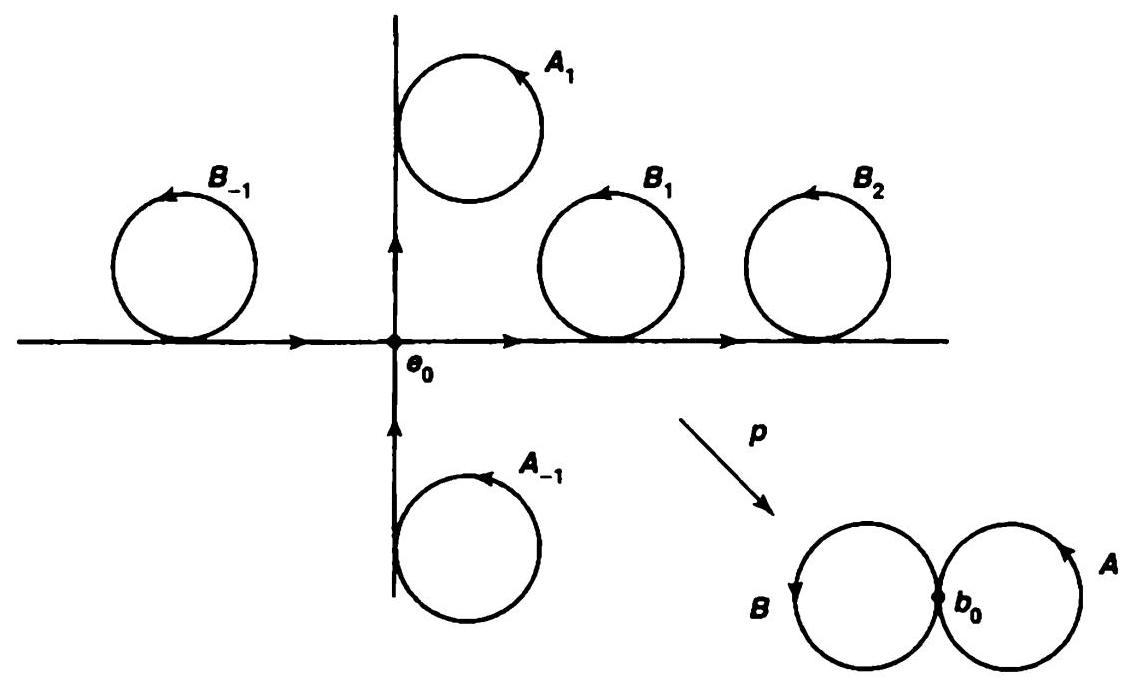
\includegraphics[width=1.0\textwidth]{images/81.2.jpg}
\end{center}
\hspace*{3em}

Figure 81.2
\end{example}
\end{centeredblock}

There is a method for constructing covering spaces that automatically leads to a covering that is regular; and in fact every \index{Regular covering space}regular covering space can be constructed by this method. It involves the action of a group \(G\) on a space \(X\) .

\begin{definition}
	Let \(X\) be a space, and let \(G\) be a subgroup of the group of homeomorphisms of \(X\) with itself. The \index{Orbit}orbit space \(X/G\) is defined to be the quotient space obtained from \(X\) by means of the equivalence relation \(x \sim  g\left( x\right)\) for all \(x \in  X\) and all \(g \in  G\) . The equivalence class of \(x\) is called the orbit of \(x\) .
\end{definition}

\begin{definition}
	If \(G\) is a group of homeomorphisms of \(X\) , the action of \(G\) on \(X\) is said to be \index{Properly discontinuous}properly discontinuous if for every \(x \in  X\) there is a neighborhood \(U\) of \(x\) such that \(g\left( U\right)\) is disjoint from \(U\) whenever \(g \neq  e\) . (Here \(e\) is the identity element of \(G\) .) It follows that \({g}_{0}\left( U\right)\) and \({g}_{1}\left( U\right)\) are disjoint whenever \({g}_{0} \neq  {g}_{1}\) , for otherwise \(U\) and \({g}_{0}^{-1}{g}_{1}\left( U\right)\) would not be disjoint.
\end{definition}

\begin{theorem}
	Let \(X\) be path connected and locally path connected; let \(G\) be a group of homeomorphisms of \(X\) . The quotient map \(\pi  : X \rightarrow  X/G\) is a covering map if and only if the action of \(G\) is properly discontinuous. In this case, the covering map \(\pi\) is regular and \(G\) is its group of covering transformations.
\end{theorem}

\begin{proof}
	We show \(\pi\) is an open map. If \(U\) is open in \(X\) , then \({\pi }^{-1}\pi \left( U\right)\) is the union of the open sets \(g\left( U\right)\) of \(X\) , for \(g \in  G\) . Hence \({\pi }^{-1}\pi \left( U\right)\) is open in \(X\) , so that \(\pi \left( U\right)\) is open in \(X/G\) by definition. Thus \(\pi\) is open.
Step 1. We suppose that the action of \(G\) is properly discontinuous and show that \(\pi\) is a covering map. Given \(x \in  X\) , let \(U\) be a neighborhood of \(x\) such that \({g}_{0}\left( U\right)\) and \({g}_{1}\left( U\right)\) are disjoint whenever \({g}_{0} \neq  {g}_{1}\) . Then \(\pi \left( U\right)\) is evenly covered by \(\pi\) . Indeed, \({\pi }^{-1}\pi \left( U\right)\) equals the union of the disjoint open sets \(g\left( U\right)\) , for \(g \in  G\) , each of which contains at most one point of each orbit. Therefore, the map \(g\left( U\right)  \rightarrow  \pi \left( U\right)\) obtained by restricting \(\pi\) is bijective; being continuous and open, it is a homeomorphism. The sets \(g\left( U\right)\) , for \(g \in  G\) , thus form a partition of \({\pi }^{-1}\pi \left( U\right)\) into slices.

Step 2. We suppose now that \(\pi\) is a covering map and show that the action of \(G\) is properly discontinuous. Given \(x \in  X\) , let \(V\) be a neighborhood of \(\pi \left( x\right)\) that is evenly covered by \(\pi\) . Partition \({\pi }^{-1}\left( V\right)\) into slices; let \({U}_{\alpha }\) be the slice containing \(x\) . Given \(g \in  G\) with \(g \neq  e\) , the set \(g\left( {U}_{\alpha }\right)\) must be disjoint from \({U}_{\alpha }\) , for otherwise, two points of \({U}_{\alpha }\) would belong to the same orbit and the restriction of \(\pi\) to \({U}_{\alpha }\) would not be injective. It follows that the action of \(G\) is properly discontinuous.

Step 3. We show that if \(\pi\) is a covering map, then \(G\) is its group of covering transformations and \(\pi\) is regular. Certainly any \(g \in  G\) is a covering transformation, for \(\pi  \circ  g = \pi\) because the orbit of \(g\left( x\right)\) equals the orbit of \(x\) . On the other hand, let \(h\) be a covering transformation with \(h\left( {x}_{1}\right)  = {x}_{2}\) , say. Because \(\pi  \circ  h = \pi\) , the points \({x}_{1}\) and \({x}_{2}\) map to the same point under \(\pi\) ; therefore there is an element \(g \in  G\) such that \(\mathrm{g}\left( {x}_{1}\right)  = {x}_{2}\) . The uniqueness part of Theorem 79.2 then implies that \(h = g\) .

It follows that \(\pi\) is regular. Indeed, for any two points \({x}_{1}\) and \({x}_{2}\) lying in the same orbit, there is an element \(g \in  G\) such that \(g\left( {x}_{1}\right)  = {x}_{2}\) . Then Corollary 81.3 applies.
\end{proof}
\begin{theorem}
	If \(p : X \rightarrow  B\) is a regular covering map and \(G\) is its group of covering transformations, then there is a homeomorphism \(k : X/G \rightarrow  B\) such that \(p = k \circ  \pi\) , where \(\pi  : X \rightarrow  X/G\) is the projection.
\end{theorem}

\begin{center}
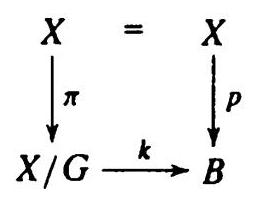
\includegraphics[width=0.2\textwidth]{images/81.25.jpg}
\end{center}
\hspace*{3em} 

\begin{proof}
	If \(g\) is a covering transformation, then \(p\left( {g\left( x\right) }\right)  = p\left( x\right)\) by definition. Hence \(p\) is constant on each orbit, so it induces a continuous map \(k\) of the quotient space \(X/G\) into \(B\) . On the other hand, \(p\) is a quotient map because it is continuous, surjective, and open. Because \(p\) is regular, any two points of \({p}^{-1}\left( b\right)\) belong to the same orbit under the action of \(G\) . Therefore, \(\pi\) induces a continuous map \(B \rightarrow  X/G\) that is an inverse for \(k\) .
\begin{centeredblock}
\begin{example}
	Let \(X\) be the cylinder \({S}^{1} \times  I\) ; let \(h : X \rightarrow  X\) be the homeomorphism \(h\left( {x,t}\right)  = \left( {-x,t}\right)\) ; and let \(k : X \rightarrow  X\) be the homeomorphism \(k\left( {x,t}\right)  = \left( {-x,1 - t}\right)\) . The groups \({G}_{1} = \{ e,h\}\) and \({G}_{2} = \{ e,k\}\) are isomorphic to the integers modulo 2; both act properly discontinuously on \(X\) . But \(X/{G}_{1}\) is homeomorphic to \(X\) , while \(X/{G}_{2}\) is homeomorphic to the Möbius band, as you can check. See Figure 81.3.

\begin{center}
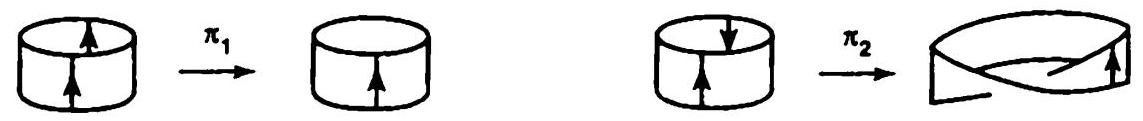
\includegraphics[width=1.0\textwidth]{images/81.3.jpg}
\end{center}
\hspace*{3em} 

Figure 81.3
\end{example}
\end{centeredblock}
\end{proof}
\section*{Exercises}
\begin{enumerate}[itemsep=0.4em, parsep=0pt, topsep=0pt, partopsep=0pt, leftmargin=*, label=\arabic*., ref=\arabic*]
\item
  \begin{enumerate}[itemsep=0.2em, parsep=0pt, topsep=0pt, partopsep=0pt, leftmargin=*, label=(\alph*), align=left]
  \item Find a group \(G\) of homeomorphisms of the torus \(T\) having order 2 such that \(T/G\) is homeomorphic to the torus.

  \item Find a group \(G\) of homeomorphisms of \(T\) having order 2 that \(T/G\) is homeomorphic to the Klein bottle.
  \end{enumerate}
\item Let \(X = A \vee  B\) be the wedge of two circles.
  \begin{enumerate}[itemsep=0.2em, parsep=0pt, topsep=0pt, partopsep=0pt, leftmargin=*, label=(\alph*), align=left]
  \item Let \(E\) be the space pictured in Figure 81.4; let \(p : E \rightarrow  X\) wrap each arc \({A}_{1}\) and \({A}_{2}\) around \(A\) and map \({B}_{1}\) and \({B}_{2}\) homeomorphically onto \(B\) . Show \(p\) is a regular covering map.
  \item Determine the group of covering transformations of the covering of \(X\) indicated in Figure 81.5 Is this covering regular? \begin{center} 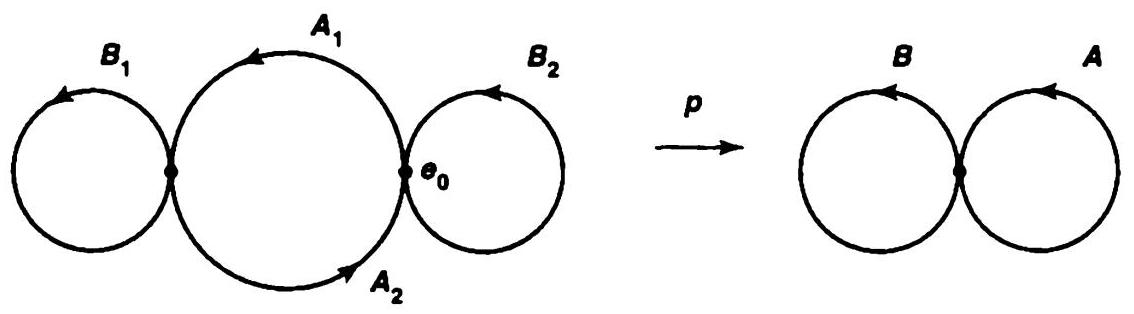
\includegraphics[width=1.0\textwidth]{images/81.4.jpg} \end{center} \hspace*{3em} Figure 81.4 \begin{center} 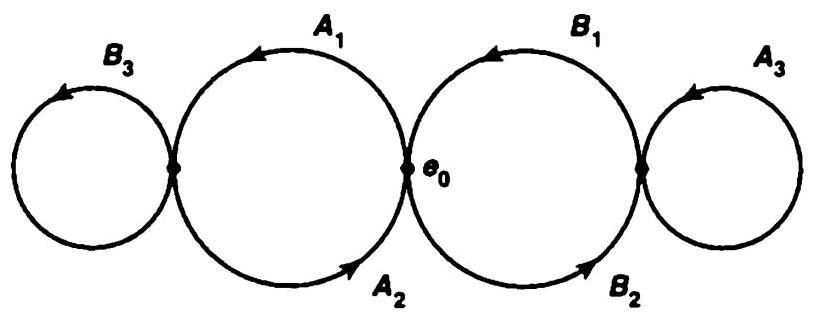
\includegraphics[width=0.7\textwidth]{images/81.5.jpg} \end{center} \hspace*{3em} Figure 81.5
  \item Repeat (b) for the covering pictured in Figure 81.6.
  \item Repeat (b) for the covering pictured in Figure 81.7. \begin{center} 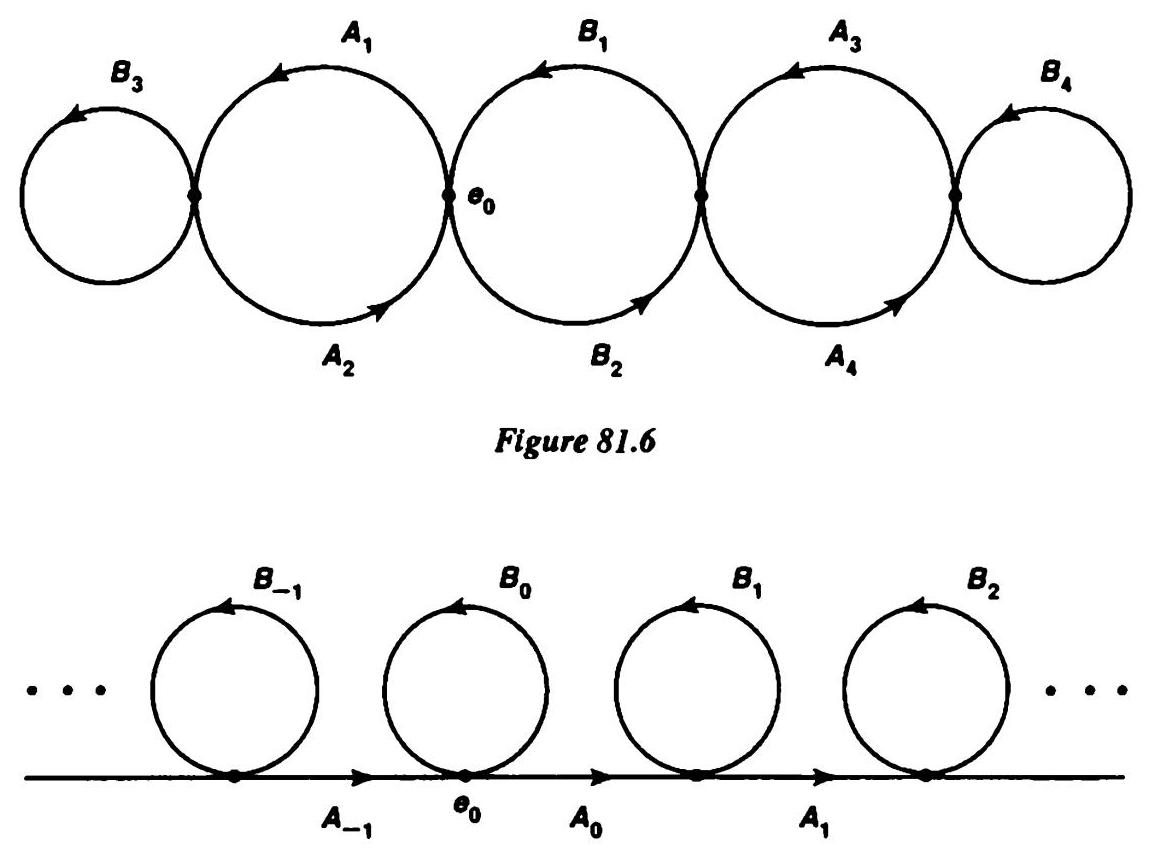
\includegraphics[width=1.0\textwidth]{images/81.6.jpg} \end{center} \hspace*{3em} Figure 81.7
  \end{enumerate}
\item Let \(p : X \rightarrow  B\) be a covering map (not necessarily regular); let \(G\) be its group of covering transformations.
  \begin{enumerate}[itemsep=0.2em, parsep=0pt, topsep=0pt, partopsep=0pt, leftmargin=*, label=(\alph*), align=left]
  \item Show that the action of \(G\) on \(X\) is properly discontinuous.
  \item Let \(\pi  : X \rightarrow  X/G\) be the projection map. Show there is a covering map \(k : X/G \rightarrow  B\) such that \(k \circ  \pi  = p\) . \begin{center} 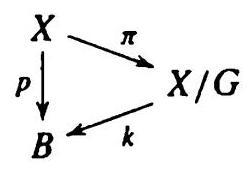
\includegraphics[width=0.2\textwidth]{images/81.7.jpg} \end{center} \hspace*{3em}
  \end{enumerate}
\item Let \(G\) be a group of homeomorphisms of \(X\) . The action of \(G\) on \(X\) is said to be fixed-point free if no element of \(G\) other than the identity \(e\) has a fixed point. Show that if \(X\) is Hausdorff, and if \(G\) is a finite group of homeomorphisms of \(X\) whose action is fixed-point free, then the action of \(G\) is properly discontinuous.
\item Consider \({S}^{3}\) as the space of all pairs of complex numbers \(\left( {{z}_{1},{z}_{2}}\right)\) satisfying the equation \({\left| {z}_{1}\right| }^{2} + {\left| {z}_{2}\right| }^{2} = 1\) . Given relatively prime positive integers \(n\) and \(k\) , define \(h : {S}^{3} \rightarrow  {S}^{3}\) by the equation \[ h\left( {{z}_{1},{z}_{2}}\right)  = \left( {{z}_{1}{e}^{{2\pi i}/n},{z}_{2}{e}^{{2\pi ik}/n}}\right) . \]
  \begin{enumerate}[itemsep=0.2em, parsep=0pt, topsep=0pt, partopsep=0pt, leftmargin=*, label=(\alph*), align=left]
  \item Show that \(h\) generates a subgroup \(G\) of the homeomorphism group of \({S}^{3}\) that is cyclic of order \(n\) , and that only the identity element of \(G\) has a fixed point. The orbit space \({S}^{3}/G\) is called the \index{Lens space}lens space \(L\left( {n,k}\right)\) .
  \item Show that if \(L\left( {n,k}\right)\) and \(L\left( {{n}^{\prime },{k}^{\prime }}\right)\) are homeomorphic, then \(n = {n}^{\prime }\) . [It is a theorem that \(L\left( {n,k}\right)\) and \(L\left( {{n}^{\prime },{k}^{\prime }}\right)\) are homeomorphic if and only if \(n = {n}^{\prime }\) and either \(k \equiv  {k}^{\prime }\left( {\;\operatorname{mod}\;n}\right)\) or \(k{k}^{\prime } \equiv  1\left( {\;\operatorname{mod}\;n}\right)\) . The proof is decidedly nontrivial.]
  \item Show that \(L\left( {n,k}\right)\) is a compact 3-manifold.
  \end{enumerate}
\item Prove the following: \textsl{Theorem.} Let \(X\) be a locally compact Hausdorff space; let \(G\) be a group of homeomorphisms of \(X\) such that the action of \(G\) is fixed-point free. Suppose that for each compact subspace \(C\) of \(X\) , there are only finitely many elements \(g\) of \(G\) such that the intersection \(C \cap  g\left( C\right)\) is nonempty. Then the action of \(G\) is properly discontinuous, and \(X/G\) is locally compact Hausdorff.  Proof.
  \begin{enumerate}[itemsep=0.2em, parsep=0pt, topsep=0pt, partopsep=0pt, leftmargin=*, label=(\alph*), align=left]
  \item For each compact subspace \(C\) of \(X\) , show that the union of the sets \(g\left( C\right)\) , for \(g \in  G\) , is closed in \(X\) . [Hint: If \(U\) is a neighborhood of \(x\) with \(\widetilde{U}\) compact, then \(\bar{U} \cup  C\) intersects \(g\left( {\bar{U} \cup  C}\right)\) for only finitely many \(g\) .]
  \item Show \(X/G\) is Hausdorff.
  \item Show the action of \(G\) is properly discontinuous.
  \item Show \(X/G\) is locally compact.
  \end{enumerate}
\end{enumerate}
\section*{§ 82 Existence of Covering Spaces}

We have shown that corresponding to each covering map \(p : E \rightarrow  B\) is a conjugacy class of subgroups of \({\pi }_{1}\left( {B,{b}_{0}}\right)\) , and that two such covering maps are equivalent if and only if they correspond to the same such class. Thus, we have an injective correspondence from equivalence classes of coverings of \(B\) to conjugacy classes of subgroups of \({\pi }_{1}\left( {B,{b}_{0}}\right)\) . Now we ask the question whether this correspondence is surjective, that is, whether for every conjugacy class of subgroups of \({\pi }_{1}\left( {B,{b}_{0}}\right)\) , there exists a covering of \(B\) that corresponds to this class.

The answer to this question is ``no,'' in general. In  \S 80, we gave an example of a path-connected, Iocally path-connected space \(B\) that had no simply connected covering space, that is, that had no covering space corresponding to the class of the trivial subgroup. This example relied on Lemma 80.4, which gave a condition that any space having a simply connected covering space must satisfy. We now introduce this condition formally.

\begin{definition}
	A space \(B\) is said to be \index{Semilocally simply connected}semilocally simply connected if for each \(b \in  B\) , there is a neighborhood \(U\) of \(b\) such that the homomorphism

\[
{i}_{ * } : {\pi }_{1}\left( {U,b}\right)  \rightarrow  {\pi }_{1}\left( {B,b}\right)
\]

induced by inclusion is trivial.
\end{definition}

Note that if \(U\) satisfies this condition, then so does any smaller neighborhood of \(b\) , so that \(b\) has ``arbitrarily small'' neighborhoods satisfying this condition. Note also that this condition is weaker than true \index{Local simple connectedness}local simple connectedness, which would require that within each neighborhood of \(b\) there should exist a neighborhood \(U\) of \(b\) that is itself simply connected.

Semilocal simple connectedness of \(B\) is both necessary and sufficient for there to exist, for every conjugacy class of subgroups of \({\pi }_{1}\left( {B,{b}_{0}}\right)\) , a corresponding covering space of \(B\) . Necessity was proved in Lemma 80.4; sufficiency is proved in this section.

\begin{theorem}
	Let \(B\) be path connected, locally path connected, and semilocally simply connected. Let \({b}_{0} \in  B\) . Given a subgroup \(H\) of \({\pi }_{1}\left( {B,{b}_{0}}\right)\) , there exists a covering map \(p : E \rightarrow  B\) and a point \({e}_{0} \in  {p}^{-1}\left( {b}_{0}\right)\) such that

\[
{p}_{ * }\left( {{\pi }_{1}\left( {E,{e}_{0}}\right) }\right)  = H
\]
\end{theorem}

\begin{proof}
	Step 1. Construction of \(E\) . The procedure for constructing \(E\) is reminiscent of the procedure used in complex analysis for constructing Riemann \index{surface with boundary@Surface with boundary}Surface with boundary surfaces. Let \(\mathcal{P}\) denote the set of all paths in \(B\) beginning at \({b}_{0}\) . Define an equivalence relation on \(\mathcal{P}\) by setting \(\alpha  \sim  \beta\) if \(\alpha\) and \(\beta\) end at the same point of \(B\) and
\[
\left\lbrack  {\alpha  * \bar{\beta }}\right\rbrack \in  H\text{ . }
\]

This relation is easily seen to be an equivalence relation. We will denote the equivalence class of the path \(\alpha\) by \({\alpha }^{\# }\) .

Let \(E\) denote the collection of equivalence classes, and define \(p : E \rightarrow  B\) by the equation

\[
p\left( {\alpha }^{\# }\right)  = \alpha \left( 1\right)
\]

Since \(B\) is path connected, \(p\) is surjective. We shall topologize \(E\) so that \(p\) is a covering map.

We first note two facts:

(1) If \(\left\lbrack  \alpha \right\rbrack = \left\lbrack  \beta \right\rbrack\) , then \({\alpha }^{\# } = {\beta }^{\# }\) .

(2) If \({\alpha }^{\# } = {\beta }^{\# }\) , then \({\left( \alpha  * \delta \right) }^{\# } = {\left( \beta  * \delta \right) }^{\# }\) for any path \(\delta\) in \(B\) beginning at \(\alpha \left( 1\right)\) .

The first follows by noting that if \(\left\lbrack  \alpha \right\rbrack = \left\lbrack  \beta \right\rbrack\) , then \(\left\lbrack  {\alpha  * \bar{\beta }}\right\rbrack\) is the identity element, which belongs to \(H\) . The second follows by noting that \(\alpha  * \delta\) and \(\beta  * \delta\) end at the same point of \(B\) , and

\[
\left\lbrack  {\left( {\alpha  * \delta }\right)  * \overline{\left( \beta  * \delta \right) }}\right\rbrack = \left\lbrack  {\left( {\alpha  * \delta }\right)  * \left( {\bar{\delta } * \bar{\beta }}\right) }\right\rbrack = \left\lbrack  {\alpha  * \bar{\beta }}\right\rbrack  ,
\]

which belongs to \(H\) by hypothesis.

Step 2. Topologizing \(E\) . One way to topologize \(E\) is to give \(\mathcal{P}\) the compact-open topology (see Chapter 7) and \(E\) the corresponding quotient topology. But we can topologize \(E\) directly as follows

Let \(\alpha\) be any element of \(\mathcal{P}\) , and let \(U\) be any path-connected neighborhood of \(\alpha \left( 1\right)\) . Define

\[
B\left( {U,\alpha }\right)  = \left\{  {{\left( \alpha  * \delta \right) }^{\# } \mid  \delta \text{ is a path in }U\text{ beginning at }\alpha \left( 1\right) }\right\}  .
\]

Note that \({\alpha }^{\# }\) is an element of \(B\left( {U,\alpha }\right)\) , since if \(b = \alpha \left( 1\right)\) , then \({\alpha }^{\# } = {\left( \alpha  * {e}_{b}\right) }^{\# }\) , this element belongs to \(B\left( {U,\alpha }\right)\) by definition. We assert that the sets \(B\left( {U,\alpha }\right)\) form a basis for a topology on \(E\) .

First, we show that if \({\beta }^{\# } \in  B\left( {U,\alpha }\right)\) , then \({\alpha }^{\# } \in  B\left( {U,\beta }\right)\) and \(B\left( {U,\alpha }\right)  = B\left( {U,\beta }\right)\) .

If \({\beta }^{\# } \in  B\left( {U,\alpha }\right)\) , then \({\beta }^{\# } = {\left( \alpha  * \delta \right) }^{\# }\) for some path \(\delta\) in \(U\) . Then

\[
\begin{aligned} {\left( \beta  * \bar{\delta }\right) }^{\# } = {\left( \left( \alpha  * \delta \right)  * \bar{\delta }\right) }^{\# }\;\text{ by (2) } &  \\ = {\alpha }^{\# }\;\text{ by }\left( 1\right) , &  \end{aligned}
\]

so that \({\alpha }^{\# } \in  B\left( {U,\beta }\right)\) by definition. See Figure 82.1. We show first that \(B\left( {U,\beta }\right)  \subset\)  \(B\left( {U,\alpha }\right)\) . Note that the general element of \(B\left( {U,\beta }\right)\) is of the form \({\left( \beta  * \gamma \right) }^{\# }\) , where \(\gamma\) is a path in \(U\) . Then note that

\[
\begin{aligned} {\left( \beta  * \gamma \right) }^{\# } = {\left( \left( \alpha  * \delta \right)  * \gamma \right) }^{\# } &  \\ = {\left( \alpha  * \left( \delta  * \gamma \right) \right) }^{\# }, &  \end{aligned}
\]

which belongs to \(B\left( {U,\alpha }\right)\) by definition. Symmetry gives the inclusion \(B\left( {U,\alpha }\right)  \subset\)  \(B\left( {U,\beta }\right)\) as well.

\begin{center}
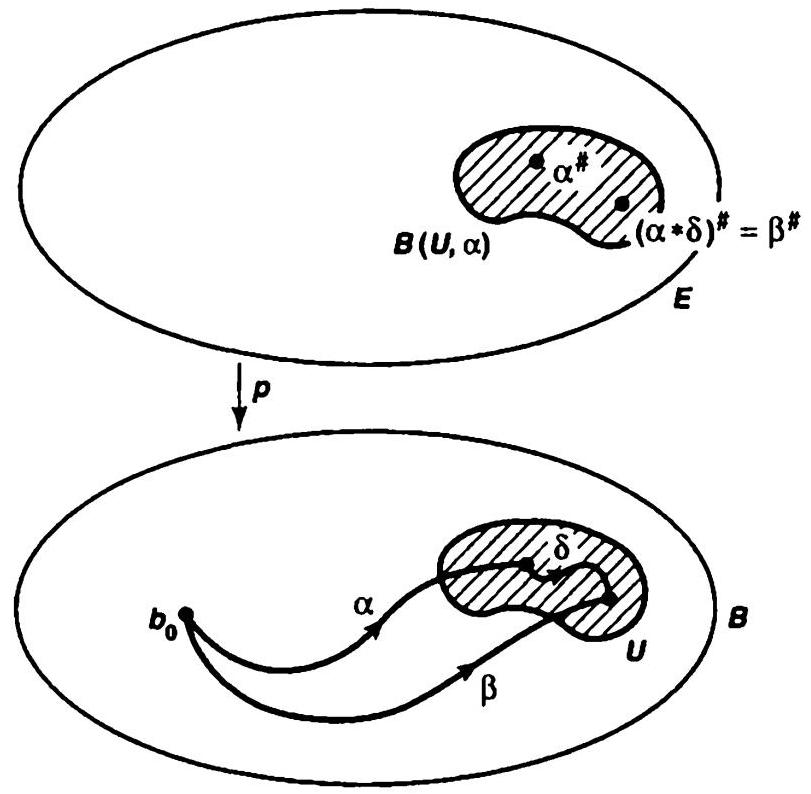
\includegraphics[width=0.7\textwidth]{images/82.1.jpg}
\end{center}
\hspace*{3em} 

Figure 82.1

Now we show the sets \(B\left( {U,\alpha }\right)\) form a basis. If \({\beta }^{\# }\) belongs to the intersection \(B\left( {{U}_{1},{\alpha }_{1}}\right)  \cap  B\left( {{U}_{2},{\alpha }_{2}}\right)\) , we need merely choose a path-connected neighborhood \(V\) of \(\beta \left( 1\right)\) contained in \({U}_{1} \cap  {U}_{2}\) . The inclusion

\[
B\left( {V,\beta }\right)  \subset  B\left( {{U}_{1},\beta }\right)  \cap  B\left( {{U}_{2},\beta }\right)
\]

follows from the definition of these sets, and the right side of the equation equals \(B\left( {{U}_{1},{\alpha }_{1}}\right)  \cap  B\left( {{U}_{2},{a}_{2}}\right)\) by the result just proved.

Step 3. The map \(p\) is continuous and open. It is easy to see that \(p\) is open, for the image of the basis element \(B\left( {U,\alpha }\right)\) is the open subset \(U\) of \(B\) : Given \(x \in  U\) , we choose a path \(\delta\) in \(U\) from \(\alpha \left( 1\right)\) to \(x\) ; then \({\left( \alpha  * \delta \right) }^{\# }\) is in \(B\left( {U,\alpha }\right)\) and \(p\left( {\left( \alpha  * \delta \right) }^{\# }\right)  = x\) .

To show that \(p\) is continuous, let us take an element \({\alpha }^{\# }\) of \(E\) and a neighborhood \(W\) of \(p\left( {\alpha }^{\# }\right)\) . Choose a path-connected neighborhood \(U\) of the point \(p\left( {\alpha }^{\# }\right)  = \alpha \left( 1\right)\) lying in \(W\) . Then \(B\left( {U,\alpha }\right)\) is a neighborhood of \({\alpha }^{\# }\) that \(p\) maps into \(W\) . Thus \(p\) is continuous at \({\alpha }^{\# }\) .

Step 4. Every point of \(B\) has a neighborhood that is evenly covered by \(p\) . Given \({b}_{1} \in  B\) , choose \(U\) to be a path-connected neighborhood of \({b}_{1}\) that satisfies the further condition that the homomorphism \({\pi }_{1}\left( {U,{b}_{1}}\right)  \rightarrow  {\pi }_{1}\left( {B,{b}_{1}}\right)\) induced by inclusion is trivial. We assert that \(U\) is evenly covered by \(p\) .

First, we show that \({p}^{-1}\left( U\right)\) equals the union of the sets \(B\left( {U,\alpha }\right)\) , as \(\alpha\) ranges over all paths in \(B\) from \({b}_{0}\) to \({b}_{1}\) . Since \(p\) maps each set \(B\left( {U,\alpha }\right)\) onto \(U\) , it is clear that \({p}^{-1}\left( U\right)\) contains this union. On the other hand, if \({\beta }^{\# }\) belongs to \({p}^{-1}\left( U\right)\) , then \(\beta \left( 1\right)  \in  U\) . Choose a path \(\delta\) in \(U\) from \({b}_{1}\) to \(\beta \left( 1\right)\) and let \(\alpha\) be the path \(\beta  * \bar{\delta }\) from \({b}_{0}\) to \({b}_{1}\) . Then \(\left\lbrack  \beta \right\rbrack = \left\lbrack  {\alpha  * \delta }\right\rbrack\) , so that \({\beta }^{\# } = {\left( \alpha  * \delta \right) }^{\# }\) , which belongs to \(B\left( {U,\alpha }\right)\) . Thus \({p}^{-1}\left( U\right)\) is contained in the union of the sets \(B\left( {U,\alpha }\right)\) .

Second, note that distinct sets \(B\left( {U,\alpha }\right)\) are disjoint. For if \({\beta }^{\# }\) belongs to \(B\left( {U,{\alpha }_{1}}\right)  \cap\)  \(B\left( {U,{\alpha }_{2}}\right)\) , then \(B\left( {U,{\alpha }_{1}}\right)  = B\left( {U,\beta }\right)  = B\left( {U,{\alpha }_{2}}\right)\) , by Step 2 .

Third, we show that \(p\) defines a bijective map of \(B\left( {U,\alpha }\right)\) with \(U\) . It follows that \(p \mid  B\left( {U,\alpha }\right)\) is a homeomorphism, being bijective and continuous and open. We already know that \(p\) maps \(B\left( {U,\alpha }\right)\) onto \(U\) . To prove injectivity, suppose that

\[
p\left( {\left( \alpha  * {\delta }_{1}\right) }^{\# }\right)  = p\left( {\left( \alpha  * {\delta }_{2}\right) }^{\# }\right) ,
\]

where \({\delta }_{1}\) and \({\delta }_{2}\) are paths in \(U\) . Then \({\delta }_{1}\left( 1\right)  = {\delta }_{2}\left( 1\right)\) . Because the homomorphism \({\pi }_{1}\left( {U,{b}_{1}}\right)  \rightarrow  {\pi }_{1}\left( {B,{b}_{1}}\right)\) induced by inclusion is trivial, \({\delta }_{1} * {\widetilde{\delta }}_{2}\) is path homotopic in \(B\) to the constant loop. Then \(\left\lbrack  {\alpha  * {\delta }_{1}}\right\rbrack = \left\lbrack  {\alpha  * {\delta }_{2}}\right\rbrack\) , so that \({\left( \alpha  * {\delta }_{1}\right) }^{\# } = {\left( \alpha  * {\delta }_{2}\right) }^{\# }\) , as desired.

It follows that \(p : E \rightarrow  B\) is a covering map in the sense used in earlier chapters. To show it is a covering map in the sense used in this chapter, we must show \(E\) is path connected. This we shall do shortly.

Step 5. Lufting a path in \(B\) . Let \({e}_{0}\) denote the equivalence class of the constant path at \({b}_{0}\) ; then \(p\left( {e}_{0}\right)  = {b}_{0}\) by definition. Given a path \(\alpha\) in \(B\) beginning at \({b}_{0}\) , we calculate its lift to a path \({mE}\) beginning at \({e}_{0}\) and show that this lift ends at \({\alpha }^{\# }\) .

To begin, given \(c \in  \left\lbrack  {0,1}\right\rbrack\) , let \({\alpha }_{c} : 1 \rightarrow  B\) denote the path defined by the equation

\[
{\alpha }_{c}\left( t\right)  = \alpha \left( {tc}\right) \;\text{ for }\;0 \leq  t \leq  1.
\]

Then \({\alpha }_{c}\) is the ``portion'' of \(\alpha\) that runs from \(\alpha \left( 0\right)\) to \(\alpha \left( c\right)\) . In particular, \({\alpha }_{0}\) is the constant path at \({b}_{0}\) , and \({\alpha }_{1}\) is the path \(\alpha\) itself. We define \(\widetilde{\alpha } : 1 \rightarrow  E\) by the equation

\[
\bar{\alpha }\left( c\right)  = {\left( {\alpha }_{c}\right) }^{\# }
\]

and show that \(\bar{\alpha }\) is continuous. Then \(\bar{\alpha }\) is a lift of \(\alpha\) , since \(p\left( {\bar{\alpha }\left( c\right) }\right)  = {\alpha }_{c}\left( 1\right)  = \alpha \left( c\right)\) ; furthermore, \(\widetilde{\alpha }\) begins at \({\left( {\alpha }_{0}\right) }^{\# } = {e}_{0}\) and ends at \({\left( {\alpha }_{1}\right) }^{\# } = {\alpha }^{\# }\) .

To verify continuity, we introduce the following notation. Given \(0 \leq  c < d \leq  1\) , let \({\delta }_{c,d}\) denote the path that equals the positive linear map of \(I\) onto \(\left\lbrack  {c,d}\right\rbrack\) followed by \(\alpha\) . Note that the paths \({\alpha }_{d}\) and \({\alpha }_{c} * {\delta }_{c,d}\) are path homotopic because one is just a reparametrization of the other. See Figure 82.2.

\begin{center}
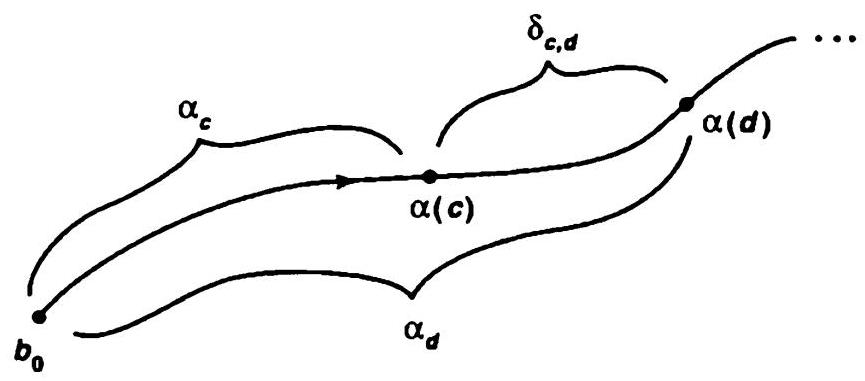
\includegraphics[width=0.8\textwidth]{images/82.2.jpg}
\end{center}
\hspace*{3em} 

Figure 82.2

We now verify continuity of \(\widetilde{\alpha }\) at the point \(c\) of \(\left\lbrack  {0,1}\right\rbrack\) . Let \(W\) be a basis element in \(E\) about the point \(\widetilde{\alpha }\left( c\right)\) . Then \(W\) equals \(B\left( {U,{\alpha }_{c}}\right)\) for some path-connected neighborhood \(U\) of \(\alpha \left( c\right)\) . Choose \(\epsilon  > 0\) so that for \(\left| {c - t}\right|  < \epsilon\) , the point \(\alpha \left( t\right)\) lies in \(U\) . We show that if \(d\) is a point of \(\left\lbrack  {0,1}\right\rbrack\) with \(\left| {c - d}\right|  < \epsilon\) , then \(\bar{\alpha }\left( d\right)  \in  W\) ; this proves continuity of \(\widetilde{\alpha }\) at \(c\) .

So suppose \(\left| {c - d}\right|  < \epsilon\) . Take first the case where \(d > c\) . Set \(\delta  = {\delta }_{c,d}\) ; then since \(\left\lbrack  {\alpha }_{d}\right\rbrack = \left\lbrack  {{\alpha }_{c} * \delta }\right\rbrack\) , we have

\[
\bar{\alpha }\left( d\right)  = {\left( {\alpha }_{d}\right) }^{\# } = {\left( {\alpha }_{c} * \delta \right) }^{\# }.
\]

Since \(\delta\) lies in \(U\) , we have \(\widetilde{\alpha }\left( d\right)  \in  B\left( {U,{\alpha }_{c}}\right)\) , as desired. If \(d < c\) , set \(\delta  = {\delta }_{d,c}\) and proceed similarly.

Step 6. The map \(p : E \rightarrow  B\) is a covering map. We need only verify that \(E\) is path connected, and this is easy. For if \({\alpha }^{\# }\) is any point of \(E\) , then the lift \(\bar{\alpha }\) of the path \(\alpha\) is a path in \(E\) from \({e}_{0}\) to \({\alpha }^{\# }\) .

Step 7. Finally, \(H = {p}_{ * }\left( {{\pi }_{1}\left( {E,{e}_{0}}\right) }\right.\) . Let \(\alpha\) be a loop in \(B\) at \({b}_{0}\) . Let \(\bar{\alpha }\) be its lift to \(E\) beginning at \({e}_{0}\) . Theorem 54.6 tells us that \(\left\lbrack  \alpha \right\rbrack \in  {p}_{ * }\left( {{\pi }_{1}\left( {E,{e}_{0}}\right) }\right)\) if and only if \(\bar{\alpha }\) is a loop in \(E\) . Now the final point of \(\widetilde{\alpha }\) is the point \({\alpha }^{\# }\) , and \({\alpha }^{\# } = {e}_{0}\) if and only if \(\alpha\) is equivalent to the constant path at \({b}_{0}\) , i.e., if and only if \(\left\lbrack  {\alpha  * {\bar{e}}_{{b}_{0}}}\right\rbrack \in  H\) This occurs precisely when \(\left\lbrack  \alpha \right\rbrack \in  H\) .
\end{proof}
\begin{corollary}
	The space \(B\) has a universal covering space if and only if \(B\) is path connected, locally path connected, and semilocally simply connected.
\end{corollary}

\section*{Exercises}
\begin{enumerate}[itemsep=0.4em, parsep=0pt, topsep=0pt, partopsep=0pt, leftmargin=*, label=\arabic*., ref=\arabic*]
\item Show that a simply connected space is semulocally simply connected.
\item Let \(X\) be the infinite earring in \({\mathbb{R}}^{2}\) . (See Example 1 of \( \S {80}\) .) Let \(C\left( X\right)\) be the subspace of \({\mathbb{R}}^{3}\) that is the union of all line segments joining points of \(X \times  0\) to the point \(p = \left( {0,0,1}\right)\) . It is called the cone on \(X\) . Show that \(C\left( X\right)\) is simply connected, but is not locally simply connected at the origin.
\end{enumerate}
\section*{* Supplementary Exercises: Topological Properties and \({\pi }_{1}\)}

The results of the preceding section tell us that the appropriate hypotheses for classifying the covering spaces of \(B\) are that \(B\) is path connected, locally path connected, and semilocally simply connected. We now show that they are also the correct hypotheses for studying the relation between various topological properties of \(B\) and the fundamental group of \(B\) .

1. Let \(X\) be a space; let \(\mathcal{A}\) be an open covering of \(X\) . Under what conditions does there exist an open covering \(\mathcal{B}\) of \(X\) refining \(\mathcal{A}\) such that for each pair \(B,{B}^{\prime }\) of elements of \(\mathcal{B}\) that have nonempty intersection, the union \(B \cup  {B}^{\prime }\) lies in an element of \(\mathcal{A}\) ?

(a) Show that such a covering \(\mathcal{B}\) exists if \(X\) is metrzable. [Hint: Choose \(\epsilon \left( x\right)\) so \(B\left( {x,{3\epsilon }\left( x\right) }\right)\) lies in an element of \(\mathcal{A}\) . Let \(\mathcal{B}\) consist of the open sets \(B\left( {x,\epsilon \left( x\right) }\right)\) .]

(b) Show that such a covering exists if \(X\) is compact Hausdorff. [Hint: Let \({A}_{1},\ldots ,{A}_{n}\) be a finite subcollection of \(\mathcal{A}\) that covers \(X\) . Choose an open covering \({C}_{1},\ldots ,{C}_{n}\) of \(X\) such that \({\bar{C}}_{i} \subset  {A}_{i}\) for each \(i\) . For each nonempty subset \(J\) of \(\{ 1,\ldots ,n\}\) , consider the set

\[
{B}_{J} = \mathop{\bigcap }\limits_{{j \in  J}}{A}_{j} - \mathop{\bigcup }\limits_{{j \notin  J}}{\bar{C}}_{j}.
\]

2. Prove the following:

\textsl{Theorem.}
	Let \(X\) be a space that is path connected, locally path connected, and semilocally simply connected. If \(X\) is regular with a countable basis, then \({\pi }_{1}\left( {X,{x}_{0}}\right)\) is countable.


\textsl{Proof.}
	Let \(\mathcal{A}\) be a covering of \(X\) by path-connected open sets \(A\) such that for each \(A \in  \mathcal{A}\) and each \(a \in  A\) , the homomorphism \({\pi }_{1}\left( {A,a}\right)  \rightarrow  {\pi }_{1}\left( {X,a}\right)\) induced by inclusion is trivial. Let \(\mathcal{B}\) be a countable open covering of \(X\) by nonempty path-connected sets that satisfies the conditions of Exercise 1. Choose a point \(p\left( B\right)  \in  B\) for each \(B \in  \mathcal{B}\) . For each pair \(B,{B}^{\prime }\) of elements of \(\mathcal{B}\) for which \(B \cap  {B}^{\prime } \neq  \varnothing\) , choose a path \(g\left( {B,{B}^{\prime }}\right)\) in \(B \cup  {B}^{\prime }\) from \(p\left( B\right)\) to \(p\left( {B}^{\prime }\right)\) . We call the path \(g\left( {B,{B}^{\prime }}\right)\) a select path.
Let \({B}_{0}\) be a fixed element of \(\mathcal{B}\) ; let \({x}_{0} = p\left( {B}_{0}\right)\) . Show that if \(f\) is a loop in \(X\) based at \({x}_{0}\) , then \(f\) is path homotopic to a product of select paths, as follows:

(a) Show that there is a subdivision

\[
0 = {t}_{0} < \cdots  < {t}_{n} = 1
\]

of \(\left\lbrack  {0,1}\right\rbrack\) such that \(f\) maps \(\left\lbrack  {{t}_{n - 1},{t}_{n}}\right\rbrack\) into \({B}_{0}\) , and for each \(i = 1,\ldots ,n - 1\) , \(f\) maps \(\left\lbrack  {{t}_{i - 1},{t}_{i}}\right\rbrack\) into an element \({B}_{i}\) of \(\mathcal{B}\) . Set \({B}_{n} = {B}_{0}\) .

(b) Let \({f}_{i}\) be the positive linear map of \(\left\lbrack  {0,1}\right\rbrack\) onto \(\left\lbrack  {{t}_{i - 1},{t}_{i}}\right\rbrack\) followed by \(f\) . Let \({g}_{i} = g\left( {{B}_{i - 1},{B}_{i}}\right)\) . Choose a path \({\alpha }_{i}\) in \({B}_{i}\) from \(f\left( {t}_{i}\right)\) to \(p\left( {B}_{i}\right)\) ; if \(\mathrm{i} = 0\) or \(n\) , let \({\alpha }_{i}\) be the constant path at \({x}_{0}\) . Show that

\[
\left\lbrack  {f}_{i}\right\rbrack * \left\lbrack  {\alpha }_{i}\right\rbrack = \left\lbrack  {\alpha }_{i - 1}\right\rbrack * \left\lbrack  {g}_{\iota }\right\rbrack  .
\]

(c) Show that \(\left\lbrack  f\right\rbrack = \left\lbrack  {g}_{1}\right\rbrack * \cdots  * \left\lbrack  {g}_{n}\right\rbrack\) .


3. Let \(p : E \rightarrow  X\) be a covering map such that \({\pi }_{1}\left( {X,{x}_{0}}\right)\) is countable. Show that if \(X\) is regular with a countable basis, so is \(E\) . [Hint: Let \(\mathcal{B}\) be a countable basis for \(X\) consisting of path-connected sets Let \(\mathcal{C}\) be the collection of path components of \({p}^{-1}\left( B\right)\) , for \(B \in  \mathcal{B}\) . Compare Exercise 6 of  \S 53.]

4. Prove the following:

\textsl{Theorem.}
	Let \(X\) be a space that is path connected, locally path connected, and semilocally simply connected. If \(X\) is compact Hausdorff, then \({\pi }_{1}\left( {X,{x}_{0}}\right)\) is finitely generated, and hence countable.


\textsl{Proof.}
	Repeat the proof outlined in Exercise 2, choosing \(\mathcal{B}\) to be finite. One has the equation
\[
\left\lbrack  f\right\rbrack = \left\lbrack  {g}_{1}\right\rbrack * \cdots  * \left\lbrack  {g}_{n}\right\rbrack  ,
\]

as before. Choose, for each \(x \in  X\) , a path \({\beta }_{x}\) from \({x}_{0}\) to \(x\) ; let \({\beta }_{{x}_{0}}\) be the constant path. If \(g = g\left( {B,{B}^{\prime }}\right)\) , define

\[
L\left( g\right)  = {\beta }_{x} * \left( {g * {\bar{\beta }}_{y}}\right) ,
\]

where \(x = p\left( B\right)\) and \(y = p\left( {B}^{\prime }\right)\) . Show that

\[
\left\lbrack  f\right\rbrack = \left\lbrack  {L\left( {g}_{1}\right) }\right\rbrack * \cdots  * \left\lbrack  {L\left( {g}_{n}\right) }\right\rbrack  .
\]

5. Let \(X\) be the infinite earnng (see Example 1 of  \S 80). Show that \(X\) is a compact Hausdorff space with a countable basis whose fundamental group is uncountable. [Hint: Let \({r}_{n} : X \rightarrow  {C}_{n}\) be a retraction. Given a sequence \({a}_{1},{a}_{2},\ldots\) of zeros and ones, show there exists a loop \(f\) in \(X\) such that, for each \(n\) , the element \({\left( {r}_{n}\right) }_{ * }\left\lbrack  f\right\rbrack\) is trivial if and only if \({a}_{n} = 0\) .]
\chapteropening[Applications to Group Theory]{Applications \\to Group Theory}

In the preceding chapter, we showed how a problem of topology---classifying all covering spaces of a space \(B\) ---can be reduced to a problem of algebra---classifying all subgroups of the fundamental group of \(B\). Now we consider the reverse process, that of reducing a problem of algebra to one of topology. The problem of algebra in question is that of showing that any subgroup of a free group is itself a free group. While this statement is certainly believable, it is not one whose proof is obvious. We shall proceed by applying the theory of covering spaces to certain topological spaces called linear graphs.

\booksection{83}{Covering Spaces of a Graph}

We define here the notion of linear graph (introduced earlier in the finite case), and prove the basic theorem that any covering space of a linear graph is itself a linear graph.

Recall that an arc \(A\) is a space homeomorphic to the unit interval \([ {0,1}]\). The end points of \(A\) are the points \(p,q\) corresponding to 0 and 1 under the homeomorphism; they are the unique points of \(A\) such that \(A - p\) and \(A - q\) are connected. The interior of an arc \(A\) consists of \(A\) with its end points deleted.

\begin{definition}
	A linear graph is a space \(X\) that is written as the union of a collection of subspaces \(A_{\alpha }\), each of which is an arc, such that:

	\begin{enumerate}[itemsep=0.2em, parsep=0pt, topsep=0pt, partopsep=0pt, leftmargin=*, label=(\arabic*), align=left]
	\item The intersection \(A_{\alpha } \cap {A}_{\beta }\) of two arcs is either empty or consists of a single point that is an end point of each.
	\item The topology of \(X\) is coherent with the subspaces \(A_{\alpha }\).
	\end{enumerate}

The arcs \(A_{\alpha }\) are called the edges of \(X\), and their interiors are called the open edges of \(X\). Their end points are called the vertices of \(X\) ; we denote the set of vertices of \(X\) by \(X^{0}\).
\end{definition}

If \(X\) is a linear graph, and if \(C\) is a subset of \(X\) that equals a union of edges and vertices of \(X\), then \(C\) is closed in \(X\). For the intersection of \(C\) with \(A_{\alpha }\) is closed in \(A_{\alpha }\), since it is either empty, or it equals \(A_{\alpha }\), or it equals one or both vertices of \(A_{\alpha }\). It follows that each edge of \(X\) is a closed subset of \(X\). It also follows that \(X^{0}\) is a closed discrete subspace of \(X\), since any subset of \(X^{0}\) is closed in \(X\).

In the case of a finite graph, considered earlier, we used the Hausdorff condition in our definition in place of condition (2); it followed, in that case, that the topology of \(X\) was coherent with the subspaces \(A_{\alpha }\). In the case of an infinite graph, this would no longer be true, so we must assume the coherence condition as part of the definition. We would assume the Hausdorff condition as well, but it is no longer necessary, for it follows from the coherence condition:

\begin{lemma}
\label{lem:\thetheorem}
Every linear graph \(X\) is Hausdorff; in fact, it is normal.
\end{lemma}

\begin{proof}
	Let \(B\) and \(C\) be disjoint closed subsets of \(X\). Assume, without loss of generality, that every vertex of \(X\) belongs either to \(B\) or to \(C\). For each \(\alpha\), choose disjoint subsets \(U_{\alpha }\) and \(V_{\alpha }\) of \(A_{\alpha }\) that are open in \(A_{\alpha }\), containing \(B \cap {A}_{\alpha }\) and \(C \cap {A}_{\alpha }\), respectively. Let \(U = \bigcup {U}_{\alpha }\) and \(V = \bigcup {V}_{\alpha }\). Then \(U\) and \(V\) contain \(B\) and \(C\), respectively.
We show the sets \(U\) and \(V\) are disjoint. If \(x \in U \cap V\), then \(x \in {U}_{\alpha } \cap {V}_{\beta }\) for some \(\alpha \neq \beta\). This fact implies that \(A_{\alpha }\) and \(A_{\beta }\) contain the point \(x\), which means that \(x\) is a vertex of \(X\). This is impossible, for if \(x \in B\), then \(x\) lies in no set \(V_{\beta }\), and if \(x \in C\), then \(x\) lies in no set \(U_{\alpha }\).

Now we show \(U\) and \(V\) are open in \(X\). To show \(U\) is open, we show that \(U \cap {A}_{\alpha } =\) \(U_{\alpha }\) for each \(\alpha\). By definition, \(U \cap {A}_{\alpha }\) contains \(U_{\alpha }\). If \(x\) is a point of \(U \cap {A}_{\alpha }\) not in \(U_{\alpha }\), then \(x\) belongs to \(U_{\beta }\) for some \(\beta \neq \alpha\). Then both \(A_{\beta }\) and \(A_{\alpha }\) contain \(x\), so that \(x\) must be a vertex of \(X\). This is impossible, for if \(x \in B\), then \(x \in {U}_{\alpha }\) by definition of \(U_{\alpha }\), and if \(x \in C\), then \(x\) cannot belong to \(U\).

\begin{centeredblock}
\begin{example}
\label{ex:\thesection.\theexample}
	If \(X\) is the wedge of the circles \(S_{\alpha }\), with common point \(p\), then \(X\) can be expressed as a linear graph. We need merely write each \(S_{\alpha }\) as a graph having three edges, with \(p\) as one of its vertices; then \(X\) is a union of arcs. To show that the topology of the wedge \(X\) is coherent with the resulting collection of arcs, we note that if \(D \cap {A}_{\alpha }\) is closed in \(A_{\alpha }\) for each arc \(A_{\alpha }\), then \(D \cap {S}_{\beta }\) is the union of three sets of the form \(D \cap {A}_{\alpha }\) and so is closed in \(S_{\beta }\) ; then \(D\) is closed in \(X\) by definition. See \hyperref[fig:83.1]{Figure 83.1}.
\end{example}
\end{centeredblock}

\begin{centeredblock}
\begin{example}
\label{ex:\thesection.\theexample}
	Let \(J\) be a discrete space, and let \(E = [ {0,1}] \times J\). Then the quotient space \(X\) obtained from \(E\) by collapsing the set \(\{ 0\} \times J\) to a point \(p\) is a linear graph.

The quotient map \(\pi : E \rightarrow X\) is a closed map. For if \(C\) is closed in \(E\), then \({\pi }^{-1}\pi ( C)\) equals \(C \cup ( {\{ 0\} \times J})\) if \(C\) contains a point of \(\{ 0\} \times J\), and \({\pi }^{-1}\pi ( C)\) equals \(C\) otherwise. In either case, \({\pi }^{-1}\pi ( C)\) is closed in \(E\), so that \(\pi ( C)\) is closed in \(X\). It follows that \(\pi\) maps each space \([ {0,1}] \times \alpha\) homeomorphically onto its image \(A_{\alpha }\), so that \(A_{\alpha }\) is an arc. The topology of \(X\) is coherent with the subspaces \(A_{\alpha }\) because \(\pi\) is a quotient map. See \hyperref[fig:83.2]{Figure 83.2}.
\end{example}
\end{centeredblock}

\munkresfig[0.3]{83.1}[Figure 83.1]
\munkresfig[0.2]{83.2}[Figure 83.2]
\end{proof}
\begin{definition}
	Let \(X\) be a linear graph. Let \(Y\) be a subspace of \(X\) that is a union of edges of \(X\). Then \(Y\) is closed in \(X\) and is itself a linear graph; we call it a subgraph of \(X\).
\end{definition}

To show that \(Y\) is a linear graph, we need to show that the subspace topology on \(Y\) is coherent with the set of edges of \(Y\). If the subset \(D\) of \(Y\) is closed in the subspace topology, then \(D\) is closed in \(X\), so that \(D \cap {A}_{\alpha }\) is closed in \(A_{\alpha }\) for each edge of \(X\), and in particular for each edge of \(Y\). Conversely, suppose \(D \cap {A}_{\beta }\) is closed in \(A_{\beta }\) for each edge \(A_{\beta }\) of \(Y\). We must show that \(D \cap {A}_{\alpha }\) is closed in \(A_{\alpha }\) for each edge \(A_{\alpha }\) of \(X\) that is not contained in \(Y\). But in this case, \(D \cap {A}_{\alpha }\) is either empty or a one-point set! We conclude that \(Y\) has the topology coherent with its set of edges.

\begin{lemma}
\label{lem:\thetheorem}
	Let \(X\) be a linear graph. If \(C\) is a compact subspace of \(X\), there exists a finite subgraph \(Y\) of \(X\) that contains \(C\). If \(C\) is connected, \(Y\) can be chosen to be connected.
\end{lemma}

\begin{proof}
	First, note that \(C\) contains only finitely many vertices of \(X\). For \(C \cap {X}^{0}\) is a closed discrete subspace of the compact space \(C\) ; since it has no limit point, it must be finite. Similarly, there are only finitely many values of \(\alpha\) for which \(C\) contains an interior point of the edge \(A_{\alpha }\). For if we choose a point \(x_{\alpha }\) of \(C\) interior to \(A_{\alpha }\) for each index \(\alpha\) for which it is possible to do so, we obtain a collection \(B = \{ x_{\alpha }\}\) whose intersection with each edge \(A_{\beta }\) is a one-point set or empty. It follows that every subset of \(B\) is closed in \(X\), so that \(B\) is a closed discrete subspace of \(C\) and hence finite.
Form \(Y\) by choosing, for each vertex \(x\) of \(X\) belonging to \(C\), an edge of \(X\) having \(x\) as a vertex, and adjoining to these edges all edges \(A_{\alpha }\) whose interiors contain points of \(C\). Then \(Y\) is a finite subgraph containing \(C\). Note that if \(C\) is connected, then \(Y\) is the union of a collection of arcs each of which intersects \(C\), so that \(Y\) is connected.
\end{proof}
\begin{lemma}
\label{lem:\thetheorem}
	If \(X\) is a linear graph, then \(X\) is locally path connected and semilocally simply connected.
\end{lemma}

\begin{proof}
	Step 1. We show \(X\) is locally path connected. If \(x \in X\) and \(x\) lies interior to some edge of \(X\), then within every neighborhood of \(x\) is a neighborhood of \(x\) homeomorphic to an open interval of \(\mathbb{R}\), which is path connected. On the other hand, if \(x\) is a vertex of \(X\) and \(U\) is a neighborhood of \(x\), then we can choose, for each edge \(A_{\alpha }\) having \(x\) as an end point, a neighborhood \(V_{\alpha }\) of \(x\) in \(A_{\alpha }\) lying in \(U\) that is homeomorphic to the half-open interval \([ {0,1}]\). Then \(\bigcup {V}_{\alpha }\) is a neighborhood of \(x\) in \(X\) lying in \(U\), and it is a union of path-connected spaces having the point \(x\) in common.
Step 2. We show \(X\) is semilocally simply connected. Indeed, we show that if \(x \in X\), then \(x\) has a neighborhood \(U\) such that \({\pi }_{1}( {U,x})\) is trivial.

If \(x\) lies interior to some edge of \(X\), then the interior of this edge is such a neighborhood. So suppose \(x\) is a vertex of \(X\). Let \(\overline{\operatorname{St}}x\) denote the union of those edges of \(X\) that have \(x\) as an end point, and let \(\operatorname{St}x\) denote the subspace of \(\overline{\operatorname{St}}x\) obtained by deleting all vertices other than \(x\). (St \(x\) is called the star of \(x\) in \(X\).) The set \(\operatorname{St}x\) is open in \(X\), since its complement is a union of arcs and vertices. We show that \({\pi }_{1}( {\operatorname{St}x, x})\) is trivial.

Let \(f\) be a loop in \(\operatorname{St}x\) based at \(x\). Then the image set \(f( I)\) is compact, so it lies in some finite union of arcs of \(\overline{\operatorname{St}}x\). Any such union is homeomorphic to the union of a finite set of line segments in the plane having an end point in common. And for any loop in such a space, the straight-line homotopy will shrink it to the constant loop at \(x\).

Now if \(x\) is a vertex of \(X\), it is in fact true that the one-point space \(\{ x\}\) is a deformation retract of \(\overline{\operatorname{St}}x\). But there is a surprising amount of effort required to show that the obvious deformation is continuous. One needs the fact that a map

\[
F : ( {\overline{\operatorname{St}}x}) \times I \rightarrow \overline{\operatorname{St}}x
\]

is continuous if its restriction to each subspace \(A_{\alpha } \times I\) is continuous. This result follows from the pasting lemma in the case where \(\overline{\operatorname{St}}x\) is a union of only finitely many arcs, but the general result requires one to show that the topology of \(( {\overline{\operatorname{St}}x}) \times I\) is coherent with the subspaces \(A_{\alpha } \times I\). This in turn follows from a basic theorem about products of quotient maps. (See Exercise 11 of \S\ 29.) These considerations do not arise if one wishes merely to shrink a loop to a point (rather than shrinking the entire space St \(x\) ), since any loop lies in the union of a finite number of edges, where there is no problem.
\end{proof}

Now we discuss covering spaces of linear graphs. Note that the convention that every covering space is assumed to be path connected and locally path connected, which we assumed in the last chapter, no longer applies.
\begin{theorem}
\label{thm:\thetheorem}
	Let \(p : E \rightarrow X\) be a covering map, where \(X\) is a linear graph. If \(A_{\alpha }\) is an edge of \(X\) and \(B\) is a path component of \(p^{-1}( A_{\alpha })\), then \(p\) maps \(B\) homeomorphically onto \(A_{\alpha }\). Furthermore, the space \(E\) is a linear graph, with the path components of the spaces \(p^{-1}( A_{\alpha })\) as its edges.
\end{theorem}

\begin{proof}
	Step 1. We show that \(p\) maps \(B\) homeomorphically onto \(A_{\alpha }\). Because the arc \(A_{\alpha }\) is path connected and locally path connected, \hyperref[thm:53.2]{Theorem 53.2} and \hyperref[lem:80.1]{Lemma 80.1} tell us that the map \(p_{0} : B \rightarrow {A}_{\alpha }\) obtained by restricting \(p\) is a covering map. Because \(B\) is path connected, the lifting correspondence \(\phi : {\pi }_{1}( {A_{\alpha },a}) \rightarrow {p}_0^{-1}( a)\) is surjective; because \(A_{\alpha }\) is simply connected, \(p_0^{-1}( a)\) consists of a single point. (See \hyperref[thm:54.4]{Theorem 54.4}.) Hence \(p_{0}\) is a homeomorphism.
Step 2. Because \(X\) is the union of the arcs \(A_{\alpha }\), the space \(E\) is the union of the arcs \(B\) that are the path components of the spaces \(p^{-1}( A_{\alpha })\). Let \(B\) and \(B^{\prime }\) be path components of \(p^{-1}( A_{\alpha })\) and \(p^{-1}( A_{\beta })\), respectively, with \(B \neq {B}^{\prime }\). We show \(B\) and \(B^{\prime }\) intersect in at most a common end point. If \(A_{\alpha }\) and \(A_{\beta }\) are equal, then \(B\) and \(B^{\prime }\) are disjoint, and if \(A_{\alpha }\) and \(A_{\beta }\) are disjoint, so are \(B\) and \(B^{\prime }\). Therefore, if \(B\) and \(B^{\prime }\) intersect, \(A_{\alpha }\) and \(A_{\beta }\) must intersect in an end point \(x\) of each; then \(B \cap {B}^{\prime }\) consists of a single point, which must be an end point of each.

Step 3. We show that \(E\) has the topology coherent with the arcs \(B\). This is the hardest part of the proof. Let \(W\) be a subset of \(E\) such that \(W \cap B\) is open in \(B\), for each arc \(B\) of \(E\). We show that \(W\) is open in \(E\).

First, we show that \(p( W)\) is open in \(X\). If \(A_{\alpha }\) is an edge of \(X\), then \(p( W) \cap {A}_{\alpha }\) is the union of the sets \(p( {W \cap B})\), as \(B\) ranges over all path components of \(p^{-1}( A_{\alpha })\). Each of these sets \(p( {W \cap B})\) is open in \(A_{\alpha }\), because \(p\) maps \(B\) homeomorphically onto \(A_{\alpha }\) ; hence their union \(p( W) \cap {A}_{\alpha }\) is open in \(A_{\alpha }\). Because \(X\) has the topology coherent with the subspaces \(A_{\alpha }\), the set \(p( W)\) is open in \(X\).

Second, we prove our result in the special case where the set \(W\) is contained in one of the slices \(V\) of \(p^{-1}( U)\), where \(U\) is an open set of \(X\) that is evenly covered by \(p\). By the result just proved, we know that the set \(p( W)\) is open in \(X\). It follows that \(p( W)\) is open in \(U\). Because the map of \(V\) onto \(U\) obtained by restricting \(p\) is a homeomorphism, \(W\) must be open in \(V\), and hence open in \(E\).

Finally, we prove our result in general. Choose a covering \(\mathcal{A}\) of \(X\) by open sets \(U\) that are evenly covered by \(p\). Then the slices \(V\) of the sets \(p^{-1}( U)\), for \(U \in \mathcal{A}\), cover \(E\). For each such slice \(V\), let \(W_{V} = W \cap V\). The set \(W_{V}\) has the property that for each arc \(B\) of \(E\), the set \(W_{V} \cap B\) is open in \(B\), for \(W_{V} \cap B = ( {W \cap B}) \cap ( {V \cap B})\) and both \(W \cap B\) and \(V \cap B\) are open in \(B\). The result of the preceding paragraph implies that \(W_{V}\) is open in \(E\). Since \(W\) is the union of the sets \(W_{V}\), it also is open in \(E\).
\end{proof}
\section*{Exercises}
\begin{enumerate}[itemsep=0.4em, parsep=0pt, topsep=0pt, partopsep=0pt, leftmargin=*, label=\arabic*., ref=\arabic*]
\item In the proof of normality of a linear graph \(X\), why did we assume that every vertex of \(X\) belongs either to \(B\) or to \(C\) ?
\item The Euler number of a finite linear graph \(X\) equals the number of vertices of \(X\) minus the number of edges of \(X\). It is in fact a topological invariant of \(X\), as we shall see. What is the Euler number of an arc? a circle? a wedge of \(n\) circles? the complete graph on \(n\) vertices? If \(E\) is an \(n\) -fold covering space of \(X\), how are the Euler numbers of \(E\) and \(X\) related?
\end{enumerate}
\booksection{84}{The Fundamental Group of a Graph}

Now we prove the basic theorem that the fundamental group of any linear graph is a free group. Henceforth we shall refer to a linear graph simply as a graph.

\begin{definition}
	An oriented edge \(e\) of a graph \(X\) is an edge of \(X\) together with an ordering of its vertices; the first is called the initial vertex, and the second, the final vertex, of e. An edge path in \(X\) is a sequence \(e_{1},\ldots ,e_{n}\) of oriented edges of \(X\) such that the final vertex of \(e_{i}\) equals the initial vertex of \(e_{i + 1}\), for \(i = 1,\ldots, n - 1\). Such an edge path is entirely specified by the sequence of vertices \(x_{0},\ldots ,x_{n}\), where \(x_{0}\) is the initial vertex of \(e_{1}\) and \(x_{i}\) is the final vertex of \(e_{i}\) for \(i = 1,\ldots, n\). It is said to be an edge path from \(x_{0}\) to \(x_{n}\). It is called a \idx[closed edge path]{Closed edge path} if \(x_{0} = x_{n}\).
\end{definition}

Given an oriented edge \(e\) of \(X\), let \(f_{e}\) be the positive linear map of \([ {0,1}]\) onto \(e\) ; it is a path from the initial point of \(e\) to the final point of \(e\). Then, corresponding to the edge path \(e_{1},\ldots ,e_{n}\) from \(x_{0}\) to \(x_{n}\), one has the actual path

\[
f = f_{1} * ( {f_{2} * ( {\cdots * f_{n}}) })
\]

from \(x_{0}\) to \(x_{n}\), where \(f_{i} = f_{e_{i}}\) ; it is uniquely determined by the edge path \(e_{1},\ldots ,e_{n}\). We call it the path corresponding to the edge path \(e_{1},\ldots ,e_{n}\). If the edge path is closed, then the corresponding path \(f\) is a loop.

\begin{lemma}
\label{lem:\thetheorem}
	A graph \(X\) is connected if and only if every pair of vertices of \(X\) can be joined by an edge path in \(X\).
\end{lemma}

\begin{proof}
	Suppose \(X\) is connected. Define \(x \sim y\) if there is an edge path in \(X\) from \(x\) to \(y\). For any edge of \(X\), its end points belong to the same equivalence class; let \(Y_{x}\) denote the union of all edges whose end points are equivalent to \(x\). Then \(Y_{x}\) is a subgraph of \(X\) and hence is closed in \(X\). The subgraphs \(Y_{x}\) form a partition of \(X\) into disjoint closed subspaces; since \(X\) is connected, there must be only one such.
Conversely, suppose every pair of vertices of \(X\) can be joined by an edge path. Then they can be joined by an actual path in \(X\). Hence all the vertices of \(X\) belong to the same component of \(X\). Since each edge is connected, it also belongs to this component. Thus \(X\) is connected.
\end{proof}
\begin{definition}
	Let \(e_{1},\ldots ,e_{n}\) be an edge path in the linear graph \(X\). It can happen that for some \(i\), the oriented edges \(e_{i}\) and \(e_{i + 1}\) consist of the same edge of \(X\), but with opposite orientations. If this situation does not occur, then the edge path is said to be a reduced edge path.
\end{definition}

Note that if this situation does occur, then one can delete \(e_{i}\) and \(e_{i + 1}\) from the sequence of oriented edges and still have an edge path remaining (provided the original sequence consists of at least three edges). This deletion process is called reducing the edge path. It enables one to show that in any connected graph, every pair of distinct vertices can be joined by a reduced edge path. See \hyperref[fig:84.1]{Figure 84.1}.

\munkresfig[0.7]{84.1}[Figure 84.1]
\begin{definition}
	A subgraph \(T\) of \(X\) is said to be a tree in \(X\) if \(T\) is connected and \(T\) contains no closed reduced edge paths.
\end{definition}

A linear graph consisting of a single edge is a tree. The graph in \hyperref[fig:84.2]{Figure 84.2} is not a tree, but deletion of the edge \(e\) would make it a tree. The graph in \hyperref[fig:84.3]{Figure 84.3} is a tree; deletion of the edge \(A\) would leave a tree remaining.

 \begin{center}
  \begin{tabular}{c@{\hspace{3em}}c}
   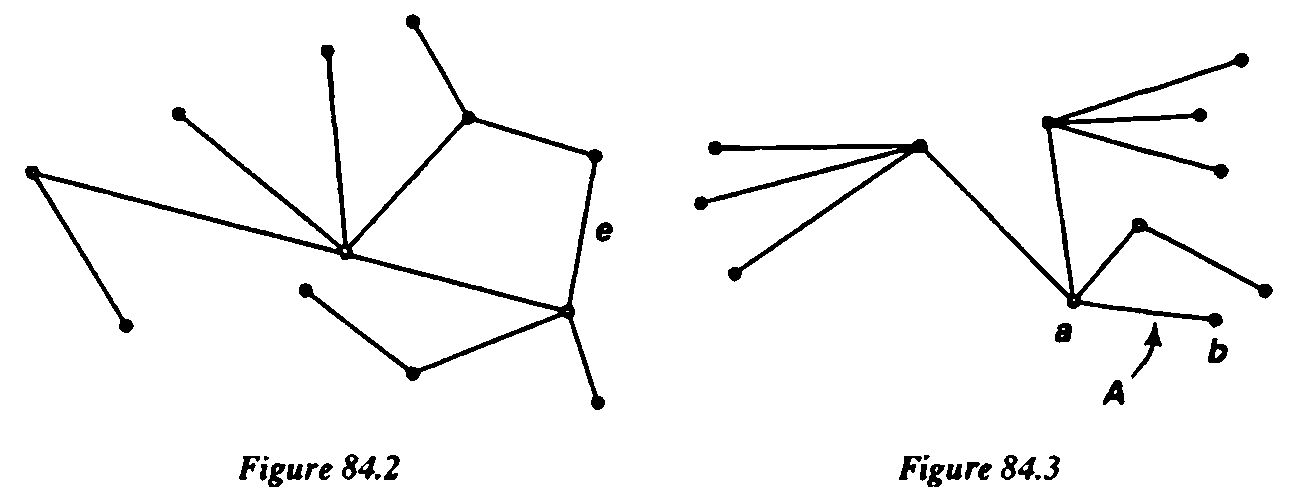
\includegraphics[width=0.45\linewidth]{images/84.2.png}\label{fig:84.2} &
   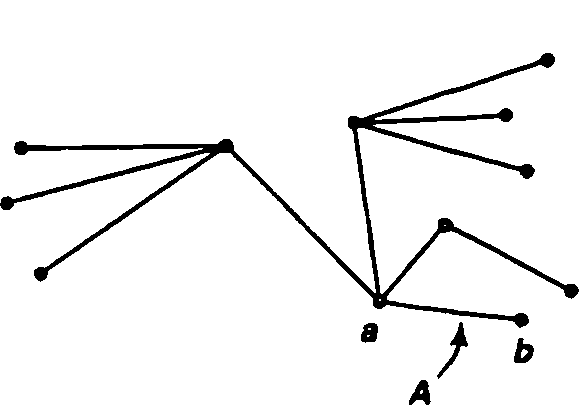
\includegraphics[width=0.45\linewidth]{images/84.3.png}\label{fig:84.3} \\[1em]
   \textbf{\textsl{Figure 84.2}} &
   \textbf{\textsl{Figure 84.3}}
  \end{tabular}
 \end{center}

\begin{lemma}
\label{lem:\thetheorem}
	If \(T\) is a tree in \(X\), and if \(A\) is an edge of \(X\) that intersects \(T\) in a single vertex, then \(T \cup A\) is a tree in \(X\). Conversely, if \(T\) is a finite tree in \(X\) that consists of more than one edge, then there is a tree \(T_{0}\) in \(X\) and an edge \(A\) of \(X\) that intersects \(T_{0}\) in a single vertex, such that \(T = T_{0} \cup A\).
\end{lemma}

\begin{proof}
	Suppose \(T\) is a tree in \(X\) and \(A\) is an edge that intersects \(T\) in a single vertex. Clearly \(T \cup A\) is connected; we show it contains no closed reduced edge paths. Let \(a\) and \(b\) be the end points of \(A\), with \(\{ a\} = T \cap A\). See \hyperref[fig:84.3]{Figure 84.3}. Suppose \(x_{0},\ldots ,x_{n} =\) \(x_{0}\) is the vertex sequence of a closed reduced edge path in \(T \cup A\). If none of the vertices \(x_{i}\) equals \(b\), then the edge path lies in \(T\), contrary to hypothesis. If \(x_{i} = b\) for some \(i\) with \(0 < i < n\), then we must have \(x_{i - 1} = a\) and \(x_{i + 1} = a\) ; hence the edge path is not reduced, contrary to hypothesis. Finally, if \(x_{0} = b = x_{n}\) and \(x_{i} \neq b\) for \(i = 1,\ldots, n - 1\), then \(x_{1} = a\) and \(x_{n - 1} = a\), and the vertex sequence \(x_{1},\ldots ,x_{n - 1}\) specifies a closed reduced edge path in \(T\), again contrary to hypothesis.
Now let \(T\) be a finite tree in \(X\) having more than one edge. First, we show that some vertex \(b\) of \(T\) belongs to only one edge of \(T\). If this is not the case, we can construct an edge path in \(T\) as follows: Begin with a vertex \(x_{0}\) of \(T\) ; then choose an edge \(e_{1}\) of \(T\) having \(x_{0}\) as an end point. Orient \(e_{1}\) so \(x_{0}\) is its initial vertex. Let \(x_{1}\) be the other end point of \(e_{1}\), and let \(e_{2}\) be an edge of \(T\) different from \(e_{1}\) having \(x_{1}\) as a vertex. Orient \(e_{2}\) so \(x_{1}\) is its initial vertex. Similarly continue. No two successive terms of the sequence \(e_{1},e_{2},\ldots\) are opposite orientations of the same edge of \(T\). Since \(T\) is finite, there must be an index \(n\) such that \(x_{n} = x_{i}\) for some \(i < n\). Then the sequence of vertices \(x_{i},x_{i + 1},\ldots ,x_{n}\) determines a closed reduced edge path in \(T\), contrary to hypothesis. See \hyperref[fig:84.4]{Figure 84.4}.

Let \(b\) be a vertex of \(T\) belonging to only one edge \(A\) of \(T\), and let \(T_{0}\) consist of all edges of \(T\) different from \(A\). Then \(T = T_{0} \cup A\). Because \(T\) is connected, \(T_{0}\) must intersect \(A\) in its other vertex \(a\). We show \(T_{0}\) is a tree. Clearly \(T_{0}\) contains no closed reduced edge paths, because \(T\) contains none. Furthermore, \(T_{0}\) is connected. For if \(T_{0}\) were the union of two disjoint closed sets \(C\) and \(D\), the point \(a\) would lie in one of them, say \(C\). Then \(C \cup A\) and \(D\) would be disjoint closed sets whose union is \(T\), contrary to the fact that \(T\) is connected.

\munkresfig[0.7]{84.4}[Figure 84.4]
\end{proof}
\begin{theorem}
\label{thm:\thetheorem}
	Any tree \(T\) is simply connected.
\end{theorem}

\begin{proof}
	We first consider the case where \(T\) is a finite tree. If \(T\) consists of a single edge, then \(T\) is simply connected. If \(T\) has \(n\) edges with \(n > 1\), there is an edge \(A\) of \(T\) such that \(T = T_{0} \cup A\), where \(T_{0}\) is a tree with \(n - 1\) edges and \(T_{0} \cap A\) is a single vertex. Then \(T_{0}\) is a deformation retract of \(T\). Since \(T_{0}\) is simply connected by the induction hypothesis, so is \(T\).
To prove the general case, let \(f\) be a loop in \(T\). The image set of \(f\) is compact and connected, so it is contained in a finite connected subgraph \(Y\) of \(T\). Now \(Y\) contains no closed reduced edge paths, because \(T\) contains none. Thus \(Y\) is a tree. Since \(Y\) is finite, it is simply connected. Hence \(f\) is path homotopic to a constant in \(Y\).
\end{proof}
\begin{definition}
	A tree \(T\) in \(X\) is maximal if there is no tree in \(X\) that properly contains \(T\).
\end{definition}

\begin{theorem}
\label{thm:\thetheorem}
	Let \(X\) be a connected graph. A tree \(T\) in \(X\) is maximal if and only if it contains all the vertices of \(X\).
\end{theorem}

\begin{proof}
	Suppose \(T\) is a tree in \(X\) that contains all the vertices of \(X\). If \(Y\) is a subgraph of \(X\) that properly contains \(T\), we show that \(Y\) contains a closed reduced edge path; it follows that \(T\) is maximal. Let \(A\) be an edge of \(Y\) that is not in \(T\) ; by hypothesis, the end points \(a\) and \(b\) of \(A\) belong to \(T\). Since \(T\) is connected, we can choose a reduced edge path \(e_{1},\ldots ,e_{n}\) in \(T\) from \(a\) to \(b\). If we follow this sequence by the edge \(A\), oriented from \(b\) to \(a\), we obtain a closed reduced edge path in \(Y\).
Now let \(T\) be a tree in \(X\) that does not contain all the vertices of \(X\). We show \(T\) is not maximal. Let \(x_{0}\) be a vertex of \(X\) not in \(T\). Since \(X\) is connected, we may choose an edge path in \(X\) from \(x_{0}\) to a vertex of \(T\), specified by the sequence of vertices \(x_{0}\), \(\ldots ,x_{n}\). Let \(i\) be the smallest index such that \(x_{i} \in T\). Let \(A\) be the edge of \(X\) with vertices \(x_{i - 1}\) and \(x_{i}\). Then \(T \cup A\) is a tree in \(X\), by the preceding lemma, and \(T \cup A\) properly contains \(T\).
\end{proof}
\begin{theorem}
\label{thm:\thetheorem}
	If \(X\) is a linear graph, every tree \(T_{0}\) in \(X\) is contained in a maximal tree in \(X\).
\end{theorem}

\begin{proof}
	We apply Zorn's lemma to the collection \(\mathcal{T}\) of all trees in \(X\) that contain \(T_{0}\), strictly partially ordered by proper inclusion. To show this collection has a maximal element, we need only prove the following:
If \(\mathcal{T}^{\prime }\) is a subcollection of \(\mathcal{T}\) that is simply ordered by proper inclusion, then the union \(Y\) of the elements of \(\mathcal{T}^{\prime }\) is a tree in \(X\).

To begin, we note that since \(Y\) is a union of subgraphs of \(X\), it is a subgraph of \(X\). Second, since \(Y\) is a union of connected spaces that contain the connected space \(T_{0}\), the space \(Y\) is connected.

Finally, we suppose that \(e_{1},\ldots ,e_{n}\) is a closed reduced edge path in \(Y\) and derive a contradiction. For each \(i\), choose an element \(T_{i}\) of \(\mathcal{T}^{\prime }\) that contains \(e_{i}\). Because \(\mathcal{T}^{\prime }\) is simply ordered by proper inclusion, one of the trees \(T_{1},\ldots ,T_{n}\), say \(T_{j}\), contains all the others. But then \(e_{1},\ldots ,e_{n}\) is a closed reduced edge path in \(T_{j}\), contrary to hypothesis.

Now we compute the fundamental group of a graph. We need the following result.
\end{proof}
\begin{lemma}
\label{lem:\thetheorem}
	Suppose \(X = U \cup V\), where \(U\) and \(V\) are open sets of \(X\). Suppose that \(U \cap V\) is the union of two disjoint open path-connected sets \(A\) and \(B\), that \(\alpha\) is a path in \(U\) from the point \(a\) of \(A\) to the point \(b\) of \(B\), and that \(\beta\) is a path in \(V\) from \(b\) to \(a\). If \(U\) and \(V\) are simply connected, then the class \([ {\alpha * \beta }]\) generates \({\pi }_{1}( {X,a})\).
\end{lemma}

\begin{proof}
	The situation is similar to that of \hyperref[thm:59.1]{Theorem 59.1}, except that \(U \cap V\) has two path components instead of one. The proof is also similar.
Let \(f\) be a loop in \(X\) based at \(a\). Choose a subdivision \(0 = a_{0} < a_{1} < \cdots < a_{n} =\) 1 of \([ {0,1}]\) such that for each \(i,f( a_{i}) \in U \cap V\) and \(f\) maps \([ {a_{i - 1},a_{i}}]\) into either \(U\) or \(V\). Let \(f_{i}\) be the positive linear map of \([ {0,1}]\) onto \([ {a_{i - 1},a_{i}}]\) followed by \(f\) ; then \([ f] = [ f_{1}] * \cdots * [ f_{n}]\). For \(i = 1,\ldots, n - 1\), choose a path \({\alpha }_{i}\) in either \(A\) or \(B\) from \(a\) or \(b\) to \(f( a_{i})\) ; choose \({\alpha }_{0}\) and \({\alpha }_{n}\) to be the constant paths at \(a\). Then set

\[
g_{i} = {\alpha }_{i - 1} * ( {f_{i} * \bar{\alpha }_{i}}).
\]

By direct computation, \([ f] = [ g_{1}] * \cdots * [ g_{n}]\). Because \(g_{i}\) is a path in \(U\) or in \(V\) with end points in the set \(\{ a,b\}\), and because \(U\) and \(V\) are simply connected, \(g_{i}\) is path homotopic either to a constant or to \(\alpha ,\beta ,\bar{\alpha }\), or \(\bar{\beta }\). It follows that either \([ f]\) is trivial, or it equals a positive power of \([ {\alpha * \beta }]\) or \([ {\bar{\beta } * \bar{\alpha }}]\). Hence \([ {\alpha * \beta }]\) generates the group \({\pi }_{1}( {X,a})\). See \hyperref[fig:84.5]{Figure 84.5}.

\munkresfig[1.0]{84.5}[Figure 84.5]
\end{proof}
\begin{theorem}
\label{thm:\thetheorem}
	Let \(X\) be a connected graph that is not a tree. Then the fundamental group of \(X\) is a nontrivial free group. Indeed, if \(T\) is a maximal tree in \(X\), then the fundamental group of \(X\) has a system of free generators that is in bijective correspondence with the collection of edges of \(X\) that are not in \(T\).
\end{theorem}

\begin{proof}
	Let \(T\) be a maximal tree in \(X\) ; it contains all the vertices of \(X\). Let \(x_{0}\) be a fixed vertex of \(T\). For each vertex \(x\) of \(X\), choose a path \({\gamma }_{x}\) in \(T\) from \(x_{0}\) to \(x\). Then for each edge \(A\) of \(X\) that is not in \(T\), define a loop \(g_{A}\) in \(X\) as follows. Orient \(A\) ; let \(f_{A}\) be the linear path in \(A\) from its initial end point \(x\) to its final end point \(y\) ; and set
\[
g_{A} = {\gamma }_{x} * ( {f_{A} * \bar{\gamma }_{y}}).
\]

We show that the classes \([ g_{A}]\) form a system of free generators for \({\pi }_{1}( {X,x_{0}})\).

Step 1. We first prove the theorem when the edges of \(X\) not in \(T\) are finite in number. We proceed by induction. The induction step is easy, so we consider it first.

Let \(A_{1},\ldots ,A_{n}\) be the edges of \(X\) not in \(T\), where \(n > 1\). Orient these edges and let \(g_{i}\) denote the loop \(g_{A_{i}}\). For each \(i\), choose a point \(p_{i}\) interior to \(A_{i}\). Let

\[
U = X - p_{2} - \cdots - p_{n}\;\text{ and }\;V = X - p_{1}.
\]

Then \(U\) and \(V\) are open in \(X\), and the space \(U \cap V = X - p_{1} - \cdots - p_{n}\) is simply connected, since it has \(T\) as a deformation retract. Therefore, \({\pi }_{1}( {X,x_{0}})\) is the free product of the groups \({\pi }_{1}( {U,x_{0}})\) and \({\pi }_{1}( {V,x_{0}})\), by \hyperref[cor:70.3]{Corollary 70.3}.

The space \(U\) has \(T \cup {A}_{1}\) as a deformation retract, so \({\pi }_{1}( {U,x_{0}})\) is free on the generator \([ g_{1}]\), as we shall prove in Step 2. The space \(V\) has \(T \cup {A}_{2} \cup \cdots \cup {A}_{n}\) as a deformation retract, so it is free on the generators \([ g_{2}] ,\ldots ,[ g_{n}]\), by the induction hypothesis. It follows from \hyperref[thm:69.2]{Theorem 69.2} that \({\pi }_{1}( {X,x_{0}})\) is free on the generators \([ g_{1}]\), \(\ldots ,[ g_{n}]\). See \hyperref[fig:84.6]{Figure 84.6}.

\munkresfig[0.7]{84.6}[Figure 84.6]
Step 2. We now consider the case where there is only one edge \(D\) of \(X\) that is not in \(T\). This step is more difficult. Orient \(D\). We show \({\pi }_{1}( {X,x_{0}})\) is infinite cyclic with generator \([ g_{D}]\).

Let \(a_{0}\) and \(a_{1}\) be the initial and final points of \(D\), respectively. Let us write \(D\) as the union of three arcs: \(D_{1}\), with end points \(a_{0}\) and \(a\), \(D_{2}\), with end points \(a\) and \(b\), and \(D_{3}\), with end points \(b\) and \(a_{1}\). See \hyperref[fig:84.7]{Figure 84.7}. Let \(f_{1},f_{2}\), and \(f_{3}\) be the linear paths in \(D\) from \(a_{0}\) to \(a\), and \(a\) to \(b\), and \(b\) to \(a_{1}\), respectively. We apply the preceding theorem to compute \({\pi }_{1}( {X,a})\).

\munkresfig[0.8]{84.7}[Figure 84.7]
Choose a point \(p\) interior to the arc \(D_{2}\). Set \(U = D - a_{0} - a_{1}\) and \(V = X - p\). Then \(U\) and \(V\) are open sets in \(X\) whose union is \(X\). The space \(U\) is simply connected because it is an open arc. And the space \(V\) is simply connected because it has the tree \(T\) as a deformation retract. The space \(U \cap V\) equals \(U - p\) ; it has two path components; let \(A\) be the one containing \(a\) and let \(B\) be the one containing \(b\). Then the hypotheses of the preceding lemma are satisfied. The path \(\alpha = f_{2}\) is a path in \(U\) from \(a\) to \(b\). If we set \({\gamma }_{0} = {\gamma }_{a_{0}}\) and \({\gamma }_{1} = {\gamma }_{a_{1}}\), then the path \(\beta = ( {f_{3} * ( {\bar{\gamma }_{1} * ( {{\gamma }_{0} * f_{1}}) }) })\) is a path in \(V\) from \(b\) to \(a\). Therefore, \({\pi }_{1}( {X,a})\) is generated by the class

\[
[ {\alpha * \beta }] = [ f_{2}] * [ f_{3}] * [ \bar{\gamma }_{1}] * [ {\gamma }_{0}] * [ f_{1}] .
\]

It follows that \({\pi }_{1}( {X,x_{0}})\) is generated by \(\widehat{\delta }[ {\alpha * \beta }]\), where \(\delta\) is the path \(\bar{f}_{1} * \bar{\gamma }_{0}\) from \(a\) to \(x_{0}\). We compute this path-homotopy class as follows:

\[
\widehat{\delta }[ {\alpha * \beta }] = [ {{\gamma }_{0} * f_{1}}] * [ {\alpha * \beta }] * [ {\bar{f}_{1} * \bar{\gamma }_{0}}]
\]

\[
= [ {\gamma }_{0}] * [ {f_{1} * ( {f_{2} * f_{3}}) }] * [ \bar{\gamma }_{1}]
\]

\[
= [ {\gamma }_{0}] * [ f_{D}] * [ \bar{\gamma }_{1}]
\]

\[
= [ g_{D}] \text{.}
\]

Therefore, \([ g_{D}]\) generates \({\pi }_{1}( {X,x_{0}})\).

It remains to show that the element \([ g_{D}]\) has infinite order, so that \({\pi }_{1}( {X,x_{0}})\) is infinite cyclic. One can apply \hyperref[thm:63.1]{Theorem 63.1} (which we used in proving the Jordan curve theorem), which states that \([ {\alpha * \beta }]\) has infinite order in \({\pi }_{1}( {X,a})\). Alternatively (and more easily), one can consider the map \(\pi : X \rightarrow {S}^{1}\) that collapses the tree \(T\) to a single point \(p\) and maps the open arc Int \(D\) homeomorphically onto \(S^{1} - p\). Then \(\pi \circ {\gamma }_{0}\) and \(\pi \circ {\bar{\gamma }}_{1}\) are constant paths, so that

\[
{\pi }_{ * }( [ g_{D}] ) = [ {\pi \circ {f}_{D}}] .
\]

This class generates \({\pi }_{1}( {S^{1},p})\). It follows that \([ g_{D}]\) has infinite order in \({\pi }_{1}( {X,x_{0}})\).

Step 3. Now we consider the situation where the collection of edges of \(X\) not in \(T\) is infinite. The proof in this case is so similar to the corresponding proof for an infinite wedge of circles that we omit the details. (See \hyperref[thm:71.3]{Theorem 71.3}.) The crucial facts are these: Any loop in \(X\) based at \(x_{0}\) lies in the space

\[
X( {{\alpha }_{1},\ldots ,{\alpha }_{n}}) = T \cup {A}_{{\alpha }_{1}} \cup \cdots \cup {A}_{{\alpha }_{n}}
\]

for some finite set of indices \({\alpha }_{i}\), and any path homotopy between such loops also lies in such a space. By this means the general case is reduced to the finite case.
\end{proof}
\section*{Exercises}
\begin{enumerate}[itemsep=0.4em, parsep=0pt, topsep=0pt, partopsep=0pt, leftmargin=*, label=\arabic*., ref=\arabic*]
\item Give an example to show that the second part of \hyperref[lem:84.2]{Lemma 84.2} need not hold if \(T\) is infinite.
\item What is the cardinality of a system of free generators for the fundamental group of the complete graph on \(n\) vertices? of the utilities graph? (See \S\ 64.)
\item Let \(X\) be the wedge of two circles; let \(p : E \rightarrow X\) be a covering map. The fundamental group of \(E\) maps isomorphically under \(p_{ * }\) onto a subgroup \(H\) of the fundamental group of \(X\) ; the latter is free on two generators \(\alpha\) and \(\beta\).
 \begin{enumerate}[itemsep=0.2em, parsep=0pt, topsep=0pt, partopsep=0pt, leftmargin=*, label=(\alph*), align=left]
 \item For each of the four covering spaces \(E\) given in Exercise 2 of \S\ 81, determine the cardinality of a system of free generators for the fundamental group of \(E\).
 \item For each of these covering spaces, find, in terms of \(\alpha\) and \(\beta\), a system of free generators for the subgroup \(H\) of the fundamental group of \(X\).
 \end{enumerate}
\end{enumerate}
\booksection{85}{Subgroups of Free Groups}

We now prove our main theorem, to the effect that a subgroup \(H\) of a free group \(F\) is free. The method of proof, remarkably enough, will give us some information about the cardinality of a system of free generators for \(H\), when the cardinality of a system of free generators for \(F\) is known.

\begin{theorem}
\label{thm:\thetheorem}
	If \(H\) is a subgroup of a free group \(F\), then \(H\) is free.
\end{theorem}

\begin{proof}
	Let \(\{ \alpha \mid \alpha \in J\}\) be a system of free generators for \(F\). Let \(X\) be a wedge of circles \(S_{\alpha }\), one for each \(\alpha \in J\) ; let \(x_{0}\) be their common point. We can give \(X\) the structure of a linear graph by breaking each circle \(S_{\alpha }\) into three arcs, two of which have \(x_{0}\) as an end point. The function that assigns to each \(\alpha\), a loop generating \({\pi }_{1}( {S_{\alpha },x_{0}})\), induces an isomorphism of \(F\) with \({\pi }_{1}( {X,x_{0}})\). Therefore we may as well assume that \(F\) equals the group \({\pi }_{1}( {X,x_{0}})\).
The space \(X\) is path connected, locally path connected, and semilocally simply connected. Therefore \hyperref[thm:82.1]{Theorem 82.1} applies to show that there exists a path-connected covering space \(p : E \rightarrow X\) of \(X\) such that, for some point \(e_{0}\) of \(p^{-1}( x_{0})\),

\[
p_{ * }( {{\pi }_{1}( {E,e_{0}}) }) = H
\]

Since \(p_{ * }\) is a monomorphism, \({\pi }_{1}( {E,e_{0}})\) is isomorphic to \(H\).

The space \(E\) is a linear graph, by \hyperref[thm:83.4]{Theorem 83.4}. Then \hyperref[thm:84.7]{Theorem 84.7} implies that its fundamental group is a free group.
\end{proof}
\begin{definition}
	If \(X\) is a finite linear graph, we define the Euler number of \(X\) to be the number of vertices of \(X\) minus the number of edges. It is commonly denoted by the Greek letter chi, as \(\chi ( X)\).
\end{definition}

\begin{lemma}
\label{lem:\thetheorem}
	If \(X\) is a finite, connected linear graph, then the cardinality of a system of free generators for the fundamental group of \(X\) is \(1 - \chi ( X)\).
\end{lemma}

\begin{proof}
	Step 1. We first show that for any finite tree \(T\), we have \(\chi ( T) = 1\). We proceed by induction on the number \(n\) of edges in \(T\). If \(n = 1\), then \(T\) has one edge and two vertices, so \(\chi ( T) = 1\). If \(n > 1\), we can write \(T = T_{0} \cup A\), where \(T_{0}\) is a tree having \(n - 1\) edges, and \(A\) is an edge that intersects \(T_{0}\) in a single vertex. We have \(\chi ( T_{0}) = 1\) by the induction hypothesis. The graph \(T\) has one more edge and one more vertex than \(T_{0}\) ; hence \(\chi ( T) = \chi ( T_{0})\).
Step 2. We prove the theorem. Given \(X\), let \(T\) be a maximal tree in \(X\). If \(X = T\), we are finished. Otherwise, let \(A_{1},\ldots ,A_{n}\) be the edges of \(X\) that are not in \(T\). Then the fundamental group of \(X\) has a system of \(n\) free generators. On the other hand, \(X\) and \(T\) have exactly the same vertex set, and \(X\) has \(n\) more edges than \(T\). Hence,

\[
\chi ( X) = \chi ( T) - n = 1 - n
\]

so that \(n = 1 - \chi ( X)\).
\end{proof}
\begin{definition}
	Let \(H\) be a subgroup of the group \(G\). If the collection \(G/H\) of right cosets of \(H\) in \(G\) is finite, its cardinality is called the index of \(H\) in \(G\). (The collection of left cosets of \(H\) in \(G\) has the same cardinality, of course.)
\end{definition}

\begin{theorem}
\label{thm:\thetheorem}
	Let \(F\) be a free group with \(n + 1\) free generators; let \(H\) be a subgroup of \(F\). If \(H\) has index \(k\) in \(F\), then \(H\) has \({kn} + 1\) free generators.
\end{theorem}

\begin{proof}
	We apply the construction given in the proof of \hyperref[thm:85.1]{Theorem 85.1}. We can assume that \(F = {\pi }_{1}( {X,x_{0}})\), where \(X\) is a linear graph whose underlying space is a wedge of \(n + 1\) circles. Given \(H\), we choose a path-connected covering space \(p : E \rightarrow X\) such that \(p_{ * }( {{\pi }_{1}( {E,e_{0}}) }) = H\). Now the lifting correspondence
\[
\Phi : {\pi }_{1}( {X,x_{0}}) /H \rightarrow {p}^{-1}( x_{0})
\]

is a bijection. Therefore, \(E\) is a \(k\) -fold covering of \(X\).

The space \(E\) is also a linear graph. Given an edge \(A\) of \(X\), the path components of \(p^{-1}( A)\) are edges of \(E\), and each is mapped by \(p\) homeomorphically onto \(A\). Thus \(E\) has \(k\) times as many edges as \(X\), and \(k\) times as many vertices. It follows that \(\chi ( E) = {k\chi }( X)\). Since the fundamental group of \(X\) has \(n + 1\) free generators, the preceding lemma tells us that \(\chi ( X) = - n\). Then the number of free generators of the fundamental group of \(E\), which is isomorphic to \(H\), is

\[
1 - \chi ( E) = 1 - {k\chi }( X) = 1 + {kn}.
\]

Note that if \(F\) is a free group with a finite system of free generators and \(H\) is a subgroup of \(F\) such that \(F/H\) is infinite, then nothing can be said about the cardinality of a system of free generators for \(H\). It might be finite (for instance, if \(H\) is the trivial subgroup) or infinite (for instance, if \(H\) is the fundamental group of the covering space pictured in \exrefs{81}{2}).
\end{proof}
\section*{Exercises}
\begin{enumerate}[itemsep=0.4em, parsep=0pt, topsep=0pt, partopsep=0pt, leftmargin=*, label=\arabic*., ref=\arabic*]
\item Show that the Euler number of a finite linear graph \(X\) is a topological invariant of \(X\). [Hint: First consider the case where \(X\) is connected.]
\item Let \(F\) be a free group on two free generators \(\alpha\) and \(\beta\). Let \(H\) be the subgroup generated by \(\alpha\). Show that \(H\) has infinite index in \(F\).
\item Let \(p : \mathbb{R} \rightarrow {S}^{1}\) be the standard covering map; consider the covering map \(p \times p : \mathbb{R} \times \mathbb{R} \rightarrow {S}^{1} \times {S}^{1}\). Let \(b_{0} = ( {1,0}) \in {S}^{1}\) ; set \(X = ( {b_{0} \times {S}^{1}}) \cup ( {S^{1} \times {b}_{0}})\) ; let \(E = {( p \times p) }^{-1}( X)\) ; and let \(q : E \rightarrow X\) be the covering map obtained by restricting \(p \times p\). The fundamental group of \(X\) has free generators \(\alpha\) and \(\beta\), where \(\alpha\) is represented by a loop in \(b_{0} \times {S}^{1}\) and \(\beta\) by a loop in \(S^{1} \times {b}_{0}\). Find a system of free generators for the subgroup \(q_{ * }( {{\pi }_{1}( {E,e_{0}}) })\), where \(e_{0}\) is the origin in \(\mathbb{R}^{2}\).
\end{enumerate}

\backmatter
\nocite{Dugundji1966}
\printbibliography
\printindex
\end{document}